%%%%%%%%%%%%%%%%%%%% book.tex %%%%%%%%%%%%%%%%%%%%%%%%%%%%%
%
% sample root file for the chapters of your "monograph"
%
% Use this file as a template for your own input.
%
%%%%%%%%%%%%%%%% Springer-Verlag %%%%%%%%%%%%%%%%%%%%%%%%%%
 
% RECOMMENDED %%%%%%%%%%%%%%%%%%%%%%%%%%%%%%%%%%%%%%%%%%%%%%%%%%%
\documentclass[graybox,envcountchap,sectrefs]{svmono}

\usepackage{mathptmx}
\usepackage{helvet}
\usepackage{courier}
%
\usepackage{type1cm}         
\usepackage{setspace}

\usepackage{xparse} 
\usepackage[table]{xcolor}
\usepackage{enumitem} 
\usepackage{mathtools}
\usepackage{ragged2e}
\usepackage{float}
\usepackage{amssymb}
\usepackage{titlesec}
\usepackage[tracking=true]{microtype}
\usepackage{changepage}
\usepackage{trimspaces}
\usepackage{bm}
\usepackage{datetime}
\usepackage{suffix}
\usepackage{nameref}
\usepackage[framemethod=TikZ]{mdframed}
\usepackage[normalem]{ulem}
\usepackage{longtable}
\usepackage[utf8]{inputenc}
\usepackage[T1]{fontenc}

\renewcommand{\ULdepth}{1.8pt}

\usepackage{makeidx}         % allows index generation
\usepackage{graphicx}        % standard LaTeX graphics tool
                             % when including figure files
\graphicspath{{Figures/}}
\usepackage{multicol}        % used for the two-column index
\usepackage[bottom]{footmisc}% places footnotes at page bottom

\usepackage[english,russian]{babel}

\babelhyphenation{иден-ти-фи-ка-то-ры}

% Курсив и жирность для кириллицы
\usepackage{substitutefont}

\substitutefont{T2A}{\familydefault}{Tempora-TLF}
\makeatletter
\input{t2atempora-tlf.fd}
\DeclareFontShape{T2A}{Tempora-TLF}{m}{sc}{
         <-> ssub * Tempora-TLF/m/n
}{}


% see the list of further useful packages
% in the Reference Guide

\makeindex             % used for the subject index
                       % please use the style svind.ist with
                       % your makeindex program

%%%%%%%%%%%%%%%%%%%%%%%%%%%%%%%%%%%%%%%%%%%%%%%%%%%%%%%%%%%%%%%%%%%%%

\usepackage{geometry}
\geometry{
  a4paper,
  left=30mm,
  right=10mm,
  top=20mm,
  bottom=15mm,
  %textwidth=117mm,
  %textheight=191mm,
  heightrounded, % <- I recommend this
  hratio=1:1,
  vratio=1:1,
}


%DEFINES START

\newcommand{\showfont}{encoding: \f@encoding{},
  family: \f@family{},
  series: \f@series{},
  shape: \f@shape{},
  size: \f@size{}
}

\newcommand\tabsize{3em}

\newlength{\insize}
\setlength{\insize}{0.7em}

\newlength{\nisize}
\setlength{\nisize}{0.7em}

\newlength{\subsetsize}
\setlength{\subsetsize}{0.8em}

\newlength{\supsetsize}
\setlength{\supsetsize}{0.8em}

\newlength{\idtfsize}
\setlength{\idtfsize}{1.1em}

\newlength{\arrowsize}
\setlength{\arrowsize}{1em}

\newlength{\bulletsize}
\setlength{\bulletsize}{0.5em}

\newlength{\bulletbracketsize}
\setlength{\bulletbracketsize}{1.15em}

\newlength{\bracketsize}
\setlength{\bracketsize}{0.4em}

\newlength{\squaresize}
\setlength{\squaresize}{0.7em}

\newlength{\doublesquaresize}
\setlength{\doublesquaresize}{1.4em}

\newlength{\eqsize}
\setlength{\eqsize}{0.8em}

\newlength{\substructsize}
\setlength{\substructsize}{1.7em}

\newcommand{\scnsupergroupsign}{\textasciicircum}
\newcommand{\scnrolesign}{\,$^\prime$}

\newcommand{\sethind}{\setlength{\hangindent}{\dimexpr (\tabsize)*\value{hind} \relax} }
\newcommand{\calctab}{\dimexpr (\tabsize)*\value{ind} \relax}
\newcommand{\settab}{\hspace{\calctab}}
\newcommand{\calcdiff}[1]{\dimexpr \tabsize-#1  \relax}
\newcommand{\makediff}[1]{\hspace{\calcdiff{#1}}}

\newcommand{\textspaced}[1]{\textls[200]{#1}}

%DEFINES END

\usepackage{tocloft}
\makeatletter
\renewcommand{\@cftmaketoctitle}{}
\makeatother
\renewcommand{\cftchapaftersnum}{.}
\renewcommand{\cftsecaftersnum}{.}
\renewcommand{\cftsubsecaftersnum}{.}
\renewcommand{\cftsubsubsecaftersnum}{.}
\renewcommand{\cftparaaftersnum}{.}
\renewcommand{\cftsubparaaftersnum}{.}
\renewcommand{\cftchapfont}{\bfseries}
\renewcommand{\cftsecfont}{\bfseries}


%SCN START

\usepackage{calc}

\newif\iffilemode
\filemodefalse

\makeatletter

\newcommand*{\trim}[1]{%
  \trim@spaces@noexp{#1}%
}

\newcounter{ind}
\newcounter{hind}
\newcounter{seg}
\newcounter{list_depth}

\newenvironment{SCn}{
\setcounter{ind}{0}
\setcounter{hind}{0} 
\setcounter{list_depth}{0} 
\begin{flushleft}
\noindent
}
{
\end{flushleft}
}

\newcommand{\scnheader}[1]{\scnresetlevel\sethind~\vspace{\parskip}\\
\textit{\textbf{#1}}\\}

\newcommand{\scnstructheader}[1]{\scnresetlevel\sethind~\vspace{\parskip}\\
\textit{\textbf{\textspaced{#1}}}\\}

\newcommand{\scnheaderlocal}[1]{\settab\textit{\textbf{#1}}\\}

\newcommand{\scnstructheaderlocal}[1]{\settab\textit{\textbf{\textspaced{#1}}}\\}

\newcommand{\scnstructidtf}[1]{\textit{\textspaced{#1}}}

\newcommand{\scnkeyword}[1]{\textit{\textbf{#1}}}

\newcommand{\scnsectionheader}[1]{\setcounter{seg}{0} \textspaced{\scnheader{\large #1}}}

\newcommand{\scnsegmentheader}[1]{
\addtocounter{seg}{1}
\ifnum\value{seg}>1
\newpage
\else
\bigskip
\fi
\scnsegmentcaption \textspaced{\scnheader{#1}}
}

\newcommand\segcountertext{
\ifnum\value{seg}=1
    Первый
\fi
\ifnum\value{seg}=2
    Второй
\fi
\ifnum\value{seg}=3
    Третий
\fi
\ifnum\value{seg}=4
    Четвертый
\fi
\ifnum\value{seg}=5
    Пятый
\fi
\ifnum\value{seg}=6
    Шестой
\fi
\ifnum\value{seg}=7
    Седьмой
\fi
\ifnum\value{seg}=8
    Восьмой
\fi
\ifnum\value{seg}=9
    Девятый
\fi
\ifnum\value{seg}=10
    Десятый
\fi
}

\makeatletter
\newcommand{\scnsegmentcaption}{\bfseries /*~Сегмент~\theseg~ Раздела~\@currentlabel.~\filldots/\hspace{0.5\textwidth}\normalfont}
\makeatother

\NewDocumentCommand\scnlist{>{\SplitList{;}}m}
   {\ProcessList{#1}{\scnlistitem}}

\NewDocumentCommand\scnrellist{>{\SplitList{;}}m}
   {\ProcessList{#1}{\scnrellistitem}}

\NewDocumentCommand\scnrolerellist{>{\SplitList{;}}m}
   {\ProcessList{#1}{\scnrolerellistitem}}

\NewDocumentCommand\scnfilelist{>{\SplitList{;}}m}
   {\ProcessList{#1}{\scnfilelistitem}}

\NewDocumentCommand\scnlistbrackets{>{\SplitList{;}}m}
   {\ProcessList{#1}{\scnlistitembrackets}}

\NewDocumentCommand\scnfilelistbrackets{>{\SplitList{;}}m}
   {\ProcessList{#1}{\scnfilelistitembrackets}}

\newcommand\scnlistitem[1]{
\sethind
\settab{$\bullet$\makediff{\bulletsize}\itshape#1} \\
}

\newcommand\scnrellistitem[1]{{\textit{#1}*{\normalfont:~}}}

\newcommand\scnrolerellistitem[1]{{\textit{#1}\scnrolesign{\normalfont:~}}}

\newcommand\scnlistitembrackets[1]{
\sethind
\settab\hspace{0.2em}\hspace{\bracketsize}{$\bullet$\makediff{\bulletbracketsize}\itshape#1}\\
}

\newcommand\scnfilelistitembrackets[1]{
\addtocounter{hind}{1}
\begin{adjustwidth}{\calctab+\tabsize+\bracketsize}{0em}
\justify
\setlength{\parskip}{0.5em}
\hspace{-\tabsize}\hspace{0.2em}\normalfont$\bullet$\makediff{\bulletbracketsize}[#1]
\setlength{\parskip}{\baselineskip}
\end{adjustwidth}
\addtocounter{hind}{-1}
}

\newcommand\scnfilelistitem[1]{
\addtocounter{hind}{1}
\begin{adjustwidth}{\calctab+\tabsize+\bracketsize}{0em}
\justify
\setlength{\parskip}{0.5em}
\hspace{-\tabsize}\hspace{-\bracketsize}\normalfont$\bullet$\makediff{\bulletsize}[#1]
\setlength{\parskip}{\baselineskip}
\end{adjustwidth}
\addtocounter{hind}{-1}
}

\newcommand\scnfileitem[1]{\scnaddlevel{1}\scnfilelong{#1}\scnaddlevel{-1}}

\newcommand\scgfileitem[1]{\scnaddlevel{1}\scnfilescg{#1}\scnaddlevel{-1}}

\newcommand{\scnrelfrom}[2]{
\settab$\bm{\Rightarrow}$\makediff{\arrowsize}\scnrellist{#1}\\
\addtocounter{ind}{1}
\addtocounter{hind}{1}
\sethind
\settab{\itshape#2}\\
\addtocounter{ind}{-1}
\addtocounter{hind}{-1}
}

\newcommand{\scnrelto}[2]{
\settab$\bm{\Leftarrow}$\makediff{\arrowsize}\scnrellist{#1}\\
\addtocounter{ind}{1}
\addtocounter{hind}{1}
\sethind 
\settab{\itshape #2}\\
\addtocounter{ind}{-1}
\addtocounter{hind}{-1}
}

\newcommand{\scnrelfromlist}[2]{
\settab$\bm{\Rightarrow}$\makediff{\arrowsize}\scnrellist{#1}\\
\addtocounter{ind}{1}
\addtocounter{hind}{1}
\addtocounter{list_depth}{1}
\ifnum\value{list_depth}=1
	\addtocounter{hind}{1}
\fi
\sethind 

\iffilemode
\scnfilelist{#2}
\else
\scnlist{#2}
\fi

\addtocounter{ind}{-1}
\ifnum\value{list_depth}=1
	\addtocounter{hind}{-1}
\fi
\addtocounter{list_depth}{-1}
\addtocounter{hind}{-1}
}

\newcommand{\scnreltolist}[2]{
\settab$\bm{\Leftarrow}$\makediff{\arrowsize}\scnrellist{#1}\\
\addtocounter{ind}{1}
\addtocounter{hind}{1}
\addtocounter{list_depth}{1}
\ifnum\value{list_depth}=1
	\addtocounter{hind}{1}
\fi
\sethind 

\iffilemode
\scnfilelist{#2}
\else
\scnlist{#2}
\fi

\addtocounter{ind}{-1}
\ifnum\value{list_depth}=1
	\addtocounter{hind}{-1}
\fi
\addtocounter{list_depth}{-1}
\addtocounter{hind}{-1}
}

\newcommand{\scnrelboth}[2]{
\settab$\bm{\Leftrightarrow}$\makediff{\arrowsize}\scnrellist{#1}\\
\addtocounter{ind}{1}
\addtocounter{hind}{1}
\sethind 
\hspace{0.2em}\settab{\itshape #2} \\
\addtocounter{hind}{-1}
\addtocounter{ind}{-1}
}

\newcommand{\scnrelbothlist}[2]{
\settab$\bm{\Leftrightarrow}$\makediff{\arrowsize}\scnrellist{#1}\\
\addtocounter{ind}{1}
\addtocounter{hind}{2}
\sethind 

\iffilemode
\scnfilelist{#2}
\else
\scnlist{#2}
\fi

\addtocounter{ind}{-1}
\addtocounter{hind}{-2}
}

\newcommand{\scnrelfromcommonset}[4]{
\settab$\bm{\Rightarrow}$\makediff{\arrowsize}\scnrellist{#3}\\
\addtocounter{ind}{1}
\addtocounter{hind}{1}
\addtocounter{list_depth}{1}
\ifnum\value{list_depth}=1
	\addtocounter{hind}{1}
\fi
\sethind 

\settab#1\\
\iffilemode
\vspace{-1.55\baselineskip}
\scnfilelistbrackets{#4}
\else
\vspace{-1\baselineskip}
\scnlistbrackets{#4}
\fi
\settab#2\\

\addtocounter{ind}{-1}
\ifnum\value{list_depth}=1
	\addtocounter{hind}{-1}
\fi
\addtocounter{list_depth}{-1}
\addtocounter{hind}{-1}
}

\newcommand{\scnrelfromset}[2]{\scnrelfromcommonset{$\pmb{\{}$}{$\pmb{\}}$}{#1}{#2}}

\newcommand{\scnrelfromvector}[2]{\scnrelfromcommonset{$\pmb{\langle}$}{$\pmb{\rangle}$}{#1}{#2}}

\newcommand{\scnreltocommonset}[4]{
\settab$\bm{\Leftarrow}$\makediff{\arrowsize}\scnrellist{#3}\\
\addtocounter{ind}{1}
\addtocounter{hind}{1}
\addtocounter{list_depth}{1}
\ifnum\value{list_depth}=1
	\addtocounter{hind}{1}
\fi
\sethind 

\settab#1\\
\iffilemode
\vspace{-1.55\baselineskip}
\scnfilelistbrackets{#4}
\else
\vspace{-1\baselineskip}
\scnlistbrackets{#4}
\fi
\settab#2\\

\addtocounter{ind}{-1}
\ifnum\value{list_depth}=1
	\addtocounter{hind}{-1}
\fi
\addtocounter{list_depth}{-1}
\addtocounter{hind}{-1}
}

\newcommand{\scnreltoset}[2]{\scnreltocommonset{$\pmb{\{}$}{$\pmb{\}}$}{#1}{#2}}

\newcommand{\scnreltovector}[2]{\scnreltocommonset{$\pmb{\langle}$}{$\pmb{\rangle}$}{#1}{#2}}

\newcommand{\scneq}[1]{
\addtocounter{hind}{1}
\sethind 
\settab$\bm{=}$\makediff{\eqsize}{\itshape #1}\\
\addtocounter{hind}{-1}
}

\newcommand{\scneqfile}[1]{
\settab$\bm{=}$\\ 
\vspace{0.5\baselineskip}
\scnfilelong{#1}
}

\newcommand{\scneqimage}[1]{
\settab$\bm{=}$\\ 
\vspace{0.5\baselineskip}
\scnfileimage{#1}
}

\newcommand{\scneqtable}[1]{
\settab$\bm{=}$\\ 
\vspace{0.5\baselineskip}
\scnfiletable{#1}
}

\newcommand{\scneqscg}[1]{
\settab$\bm{=}$\\ 
\vspace{0.5\baselineskip}
\scnfilescg{#1}
}

\newcommand{\scneqfileclass}[1]{
\settab$\bm{=}$\makediff{\eqsize}\scnfileclass{#1}\\
}

\newcommand{\scneqtocommonset}[3]{
\settab$\bm{=}$\makediff{\eqsize}#1\\
\addtocounter{ind}{1}
\addtocounter{hind}{2}
\sethind 
\iffilemode
\vspace{-1.55\baselineskip}
\scnfilelistbrackets{#3}
\else
\vspace{-1\baselineskip}
\scnlistbrackets{#3}
\fi
\settab#2\\
\addtocounter{ind}{-1}
\addtocounter{hind}{-2}
}

\newcommand{\scneqtoset}[1]{\scneqtocommonset{$\pmb{\{}$}{$\pmb{\}}$}{#1}}

\newcommand{\scneqtovector}[1]{\scneqtocommonset{$\pmb{\langle}$}{$\pmb{\rangle}$}{#1}}

\newcommand{\scnhassubstruct}[1]{
\settab$\bm{\supset=}$\makediff{\substructsize}$\pmb{\{}$\\
\addtocounter{ind}{1}
\addtocounter{hind}{2}
\sethind 
\iffilemode
\vspace{-1.55\baselineskip}
\scnfilelistbrackets{#1}
\else
\vspace{-1\baselineskip}
\scnlistbrackets{#1}
\fi
\settab$\pmb{\}}$\\
\addtocounter{ind}{-1}
\addtocounter{hind}{-2}
}

\newcommand{\scnsubset}[1]{
\addtocounter{hind}{1}
\sethind 
\settab$\bm{\subset}$\makediff{\subsetsize}{\itshape #1}\\
\addtocounter{hind}{-1}
}

\newcommand{\scnsuperset}[1]{
\addtocounter{hind}{1}
\sethind 
\settab$\bm{\supset}$\makediff{\supsetsize}{\itshape #1}\\
\addtocounter{hind}{-1}
}

\newcommand{\scniselement}[1]{
\addtocounter{hind}{1}
\sethind
\settab$\bm{\in}$\hspace{\calcdiff{\insize}}{\itshape #1}\\
\addtocounter{hind}{-1}
}

\newcommand{\scnmakesetlocal}[1]{
\hspace{-\bracketsize}$\pmb{\{}$\\
\addtocounter{ind}{1}
\addtocounter{hind}{2}
\sethind 
\vspace{-1\baselineskip}
\scnlistbrackets{#1}
\settab$\pmb{\}}$\\
\addtocounter{ind}{-1}
\addtocounter{hind}{-2}
}

\newcommand{\scnmakeset}[1]{
\settab$\pmb{\{}$\\
\sethind 
\vspace{-1\baselineskip}
\scnlistbrackets{#1}
\settab$\pmb{\}}$\\
}

\newcommand{\scnhaselementset}[1]{
\settab$\bm{\ni}$\makediff{\nisize}\scnmakesetlocal{#1}
}

\newcommand{\scnhaselement}[1]{
\addtocounter{hind}{1}
\sethind 
\settab$\bm{\ni}$\makediff{\nisize}{\itshape #1}\\
\addtocounter{hind}{-1}
}

\newcommand{\scnhaselements}[1]{
\addtocounter{hind}{1}
\sethind 
\settab$\bm{\ni}$\makediff{\nisize}#1\\
\addtocounter{hind}{-1}
}

\newcommand{\scnsubdividing}[1]{\scnrelfromset{разбиение}{#1}}

\newcommand{\scnhaselementrole}[2]{
\settab$\bm{\ni}$\makediff{\nisize}\scnrolerellist{#1}\\
\addtocounter{ind}{1}
\addtocounter{hind}{1}
\sethind 
\settab{\itshape #2}\\
\addtocounter{ind}{-1}
\addtocounter{hind}{-1}
}

\newcommand{\scnhaselementlist}[2]{
\settab$\bm{\ni}$\makediff{\nisize}\scnrolerellist{#1}\\
\addtocounter{ind}{1}
\addtocounter{hind}{2}
\sethind 
\scnlist{#2}
\addtocounter{ind}{-1}
\addtocounter{hind}{-2}
}

\newcommand{\scniselementrole}[2]{
\settab$\bm{\in}$\makediff{\insize}\scnrolerellist{#1}\\
\addtocounter{ind}{1}
\addtocounter{hind}{1}
\sethind 
\settab{\itshape #2}\\
\addtocounter{ind}{-1}
\addtocounter{hind}{-1}
}

\newcommand{\scnrole}[1]{{\itshape #1\scnrolesign}:}

\newcommand{\scnset}[1]{$\pmb{\{}$#1$\pmb{\}}$}
\newcommand{\scnvector}[1]{$\pmb{\langle}$#1$\pmb{\rangle}$}

\newcommand{\scnidtf}[1]{
\begin{adjustwidth}{\calctab+3.4em}{0em}
\justify
\hspace{-3.4em}\normalfont $\bm{\coloneqq}$\hspace{\calcdiff{\idtfsize}}[#1]
\end{adjustwidth}
}

\newcommand{\scnidtftext}[2]{
\settab$\bm{\coloneqq}$\hspace{\calcdiff{\idtfsize}}\scnrellist{#1}\\
\addtocounter{ind}{1}
\settab{\scnfilelong{#2}}\\
\addtocounter{ind}{-1}
}

\newcommand{\scnidtfdef}[1]{\scnidtftext{определение}{#1}}

\newcommand{\scnidtfexp}[1]{\scnidtftext{пояснение}{#1}}

\newcommand{\scnaddlevel}[1]{
\addtocounter{ind}{#1}
\addtocounter{hind}{#1}}

\newcommand{\scnaddhind}[1]{
\addtocounter{hind}{#1}}

\newcommand{\scnresetlevel}{
\setcounter{ind}{0}
\setcounter{hind}{0}}

\newcommand{\scnfileshort}[1]{
{\normalfont [#1]}
}

\newcommand{\scnfileclass}[1]{
{\normalfont\hspace{-0.3em}![~#1~]!}
}

\newcommand{\scnfilelong}[1]{
\begin{adjustwidth}{\calctab+0.4em}{0em}
\justify
\setlength{\parindent}{0em}
\setlength{\itemindent}{0em}
\setlength{\parskip}{0.5em}
\vspace{-1.5em}
\hspace{-0.4em}\normalfont \textbf{[}#1\textbf{]}
\end{adjustwidth}
}

\usepackage{tabularx}

\newcommand{\scnfileimage}[1]{
\begin{adjustwidth}{\calctab}{0em}
\setlength{\parindent}{0em}
\setlength{\itemindent}{0em}
\setlength{\parskip}{0.5em}
\vspace{-1.5em}
\normalfont \textbf{[}
\setlength\arrayrulewidth{1pt}
\hspace{0.1em}\begin{tabularx}{\textwidth-\calctab}{X}
\cellcolor{white}\begin{center}\vspace{-1.3\baselineskip}#1\vspace{-0.7\baselineskip}\end{center}
\end{tabularx}
\textbf{]}
\end{adjustwidth}
}

\newcommand{\scnfiletable}[1]{
\begin{adjustwidth}{\calctab}{0em}
\setlength{\parindent}{0em}
\setlength{\itemindent}{0em}
\setlength{\parskip}{0.5em}
\vspace{-1.5em}
\normalfont \textbf{[}
\setlength\arrayrulewidth{1pt}
\hspace{0.1em}\begin{tabularx}{\textwidth-\calctab}{X}
#1
\end{tabularx}
\textbf{]}
\end{adjustwidth}
}

\newcommand{\scnfilescg}[1]{
\begin{adjustwidth}{\calctab}{0em}
\setlength{\parindent}{0em}
\setlength{\itemindent}{0em}
\setlength{\parskip}{0.5em}
\vspace{-1.5em}
\normalfont \textbf{[}
\setlength\arrayrulewidth{1pt}
\hspace{0.1em}\begin{tabularx}{\textwidth-\calctab}{X}
\cellcolor{white}\begin{center}\vspace{-1.3\baselineskip}\includegraphics[scale=0.8]{#1}\vspace{-0.7\baselineskip}\end{center}
\end{tabularx}
\textbf{]}
\end{adjustwidth}
}

\newcommand{\scnstartsubstruct}{
\settab$\pmb{\supset=}$\\
\settab$\pmb{\{}$
}

\newcommand{\scnstructinclusion}{
\settab$\pmb{\supset=}$\\
}

\newcommand{\scnstartstruct}{\settab$\pmb{=\{}$}
\newcommand{\scnstartset}{\settab$\pmb{\{}$}
\newcommand{\scnstartsetlocal}{$\pmb{\{}$}
\newcommand{\scnendstruct}{\settab$\pmb{\}}$}

\newcommand{\scnendstructlocal}{$\pmb{\}}$}

\newcommand{\scnstartfile}{\settab\textbf{=}\\
\settab\textbf{[}\\}

\newcommand{\scnendfile}{\settab\textbf{]}}


\newcommand{\scnfilelongbreaks}[1]
{\scnfilelong{\\#1\\}}

\newcommand{\scntext}[2]{
\scnrelfrom{#1}{\scnfilelong{#2}}
}

\newcommand{\scncomment}[1]{
\scntext{комментарий}{#1}
}

\newcommand{\scnexplanation}[1]{
\scntext{пояснение}{#1}
}

\newcommand{\scnnote}[1]{
\scntext{примечание}{#1}
}

\newcommand{\scndefinition}[1]{
\scntext{определение}{#1}
}

\newcommand{\scnevolution}[1]{
\scntext{эволюция}{#1}
}

\newcommand{\scnproblems}[1]{
\scntext{проблемы}{#1}
}

\newcommand{\scnevolutiondirections}[1]{
\scntext{направления эволюции}{#1}
}

\newcommand{\scnevolutionproblems}[1]{
\scntext{проблемы развития}{#1}
}

\newcommand{\scnmodernstate}[1]{
\scntext{современное состояние}{#1}
}

\newcommand{\scnsolutionapproach}[1]{
\scntext{предлагаемый подход к решению}{#1}
}

\newcommand{\scnadvantages}[1]{
\scntext{достоинства}{#1}
}

\newcommand{\scnprinciples}[1]{
\scntext{принципы}{#1}
}

\newcommand{\scnspheresapplication}[1]{
\scntext{сферы применения}{#1}
}

\newcommand{\scnseminclusion}[1]{
\scntext{семантическое включение}{#1}
}

\newcommand{\scnsourcecomment}[1]{{\normalfont \normalsize \textbf{/*~}#1\textbf{{}~*/}}}

\newcommand{\scnsourcecommentpar}[1]{
\begin{adjustwidth}{\calctab+1em}{0em}
\justify
\setlength{\parindent}{0em}
\setlength{\itemindent}{0em}
\hspace{-1em}\normalfont /*~#1{}~*/
\end{adjustwidth}
}

\newcommand{\scninlinesourcecommentpar}[1]{
\begin{adjustwidth}{\calctab+1em+\tabsize}{0em}
\justify
\setlength{\parindent}{0em}
\setlength{\itemindent}{0em}
\vspace{-0.9\baselineskip}
\hspace{-1em}\normalfont /*~#1{}~*/
\end{adjustwidth}
}

\newcommand{\scnauthorcomment}[1]{\begin{flushleft}
/*/*#1*/*/\end{flushleft}}

\newenvironment{FileFrame}{
\begin{mdframed}[linewidth=0.5mm,roundcorner=0pt]
}
{
\end{mdframed}
}

\newenvironment{ContourFrame}{
\begin{mdframed}[linewidth=0.5mm,roundcorner=20pt]
}
{
\end{mdframed}
}

%Subject domains
\newcommand{\scnsdmainclass}[1]{
\scnhaselementlist{максимальный класс объектов исследования}{#1}
}

\newcommand{\scnsdmainclasssingle}[1]{
\scnhaselementrole{максимальный класс объектов исследования}{#1}
}

\newcommand{\scnsdclass}[1]{
\scnhaselementlist{класс объектов исследования}{#1}
}

\newcommand{\scnsdrelation}[1]{
\scnhaselementlist{исследуемое отношение}{#1}
}

\newcommand{\timestamp}{\vspace{0.5em}\scnauthorcomment{\textbf{\large Версия от \today~ \currenttime}}}

\newcommand{\addedstart}{\reversemarginpar\marginpar{\hspace{3em}НОВОЕ~[}}

\newcommand{\addedend}{\reversemarginpar\marginpar{\hspace{3em}]~НОВОЕ}}

\newcommand{\editedstart}{\reversemarginpar\marginpar{\hspace{3em}ИЗМЕНЕНО~[}}

\newcommand{\editedend}{\reversemarginpar\marginpar{\hspace{3em}]~ИЗМЕНЕНО}}


\makeatother

%SCN END

%Sections START

\titleformat{\chapter}[display]
{\normalfont\bfseries}{}{0pt}{\normalsize}

\titleformat{\section}[display]
{\normalfont\bfseries}{}{0pt}{\normalsize}

\titleformat{\subsection}[display]
{\normalfont\bfseries}{}{0pt}{\normalsize}

\titleformat{\subsubsection}[display]
{\normalfont\bfseries}{}{0pt}{\normalsize}

\titleformat{\paragraph}[display]
{\normalfont\bfseries}{}{0pt}{\normalsize}

\titlespacing*{\chapter}
{0em}{0em}{0em}
\titlespacing*{\section}
{0em}{0em}{0em}
\titlespacing*{\subsection}
{0em}{0em}{0em}
\titlespacing*{\subsubsection}
{0em}{0em}{0em}
\titlespacing*{\paragraph}
{0em}{0em}{0em}

\newcommand{\filldots}{\xleaders\hbox{*}\hfill}
\newlength\afterparlength
\setlength{\afterparlength}{-2em}

\newcommand{\scsuperchapter}{{\normalfont\bfseries\large/*\filldots/}\vspace{0.5\afterparlength}}

\newcommand{\scchapter}[1]{\clearpage
\chapter[\textit{#1}]{/*~Раздел~ \thechapter~\filldots/\vspace{\afterparlength}}}

\newcommand{\scsection}[1]{\clearpage
\section[\textit{#1}]{/*~Раздел~\thesection~\filldots/\vspace{\afterparlength}}}

\newcommand\scsubsection[1]{\clearpage
\subsection[\textit{#1}]{/*~Раздел~ \thesubsection~\filldots/\vspace{\afterparlength}}}

\WithSuffix\newcommand\scsubsection*[2]{\clearpage\subsection*{/*~Раздел~ #2~\filldots/\vspace{\afterparlength}}
\addcontentsline{toc}{subsection}{#1}
}

\newcommand{\scsubsubsection}[1]{\clearpage
\subsubsection[\textit{#1}]{/*~Раздел~ \thesubsubsection~\filldots/\vspace{\afterparlength}}}

\WithSuffix\newcommand\scsubsubsection*[2]{\clearpage\subsubsection*{/*~Раздел~#2~\filldots/\vspace{\afterparlength}}
\addcontentsline{toc}{subsubsection}{#1}
}

\newcommand{\scparagraph}[1]{\clearpage
\paragraph[\textit{#1}]{/*~Раздел~\theparagraph~\filldots/\vspace{\afterparlength}}}

\newcommand{\scchapterfinish}[1]{\clearpage
\section*{/*~Завершение раздела~\ref{#1}~\filldots/\vspace{\afterparlength}}}

\newcommand{\scsectionfinish}[1]{\clearpage
\section*{/*~Завершение раздела~\ref{#1}~\filldots/\vspace{\afterparlength}}}

\newcommand{\scsubsectionfinish}[1]{\clearpage
\subsection*{/*~Завершение раздела~\ref{#1}~\filldots/\vspace{\afterparlength}}}

\newcommand{\scsubsubsectionfinish}[1]{\clearpage
\subsubsection*{/*~Завершение раздела~\ref{#1}~\filldots/\vspace{\afterparlength}}}

\makeatletter
\newcommand{\scsectionbeginning}{\bigskip
{\bfseries \normalsize /*~Начало  Раздела~\@currentlabel~\filldots/\hspace{0.5\textwidth}\normalfont}
\scnsectionheader{Начало Раздела "\@currentlabelname"}
}
\makeatother

\makeatletter
\newcommand{\scsectionbeginningname}[1]{\bigskip
{\bfseries \normalsize /*~Начало  Раздела~\@currentlabel~\filldots/\hspace{0.5\textwidth}\normalfont}
\scnsectionheader{#1}
}
\makeatother

\newcommand{\scsupersectionbeginning}[1]{\bigskip \section*{\bfseries /*~Начало.~\filldots/\hspace{0.5\textwidth}}
\vspace{0.5\afterparlength}
\scnsectionheader{Начало Документации Технологии OSTIS}
}

\makeatletter
\newcommand*{\currentname}{\@currentlabelname}
\makeatother

\makeatletter
\newcommand*{\currentnumber}{\@currentlabel}
\makeatother

%Sections END

% Itemize START

\newenvironment{scnitemize}{
\begin{itemize}[leftmargin=\leftmargin-1em+\bracketsize,itemsep=-0.25em,before=\vspace{-0.8em},after=\vspace{-0.5em}]
\renewcommand{\labelitemi}{\scriptsize$\square$}
\renewcommand{\labelitemii}{\scriptsize$\square~\square$}
\renewcommand{\labelitemiii}{\scriptsize$\square~\square~\square$} 
}
{
\end{itemize}
}

\newenvironment{scnitemizeii}{
\begin{itemize}[leftmargin=\leftmargin-1em+\bracketsize+\squaresize,itemsep=-0.25em,before=\vspace{-0.3em},after=\vspace{0em}]
\renewcommand{\labelitemi}{\scriptsize$\square~\square$} 
}
{
\end{itemize}
}

\newenvironment{scnitemizeiii}{
\begin{itemize}[leftmargin=\leftmargin-1em+\bracketsize+\doublesquaresize,itemsep=-0.25em,before=\vspace{-0.3em},after=\vspace{0em}]

\renewcommand{\labelitemi}{\scriptsize$\square~\square$} 
}
{
\end{itemize}
}

\newenvironment{scnenumerate}{
\begin{enumerate}[leftmargin=\leftmargin-1em+\bracketsize,itemsep=-0.25em,before=\vspace{-0.8em},after=\vspace{-0.5em}]
}
{
\end{enumerate}
}

\newcommand{\scncontentname}{\begin{SCn}
\scnsectionheader{Оглавление описания Технологии OSTIS}
$\bm{=[}$
\end{SCn}}

% Itemize END


% Background START

\usepackage[pages=all]{background}
\usepackage{tikz}
\usetikzlibrary{calc} 
\usepackage{layout}

\newcommand{\drawvlines}{
\begin{tikzpicture}[remember picture,overlay]

\coordinate (NW) at ([
            xshift=0.75in,
            yshift=-1.1in-2\voffset-\topmargin-\headheight-\headsep,
        ]current page.north west);
        
\coordinate (SW) at ([
            xshift=0.75in,
            yshift=-1.1in-2\voffset-\topmargin-\headheight-\headsep-\textheight,
        ]current page.north west);

\foreach \i in {1,2,...,25}{
\draw[gray] ($(NW)+(\i*\tabsize,0)$) -- ($(SW)+(\i*\tabsize,0)$);}

\end{tikzpicture}
}

\newcommand\DeactivateBG{\backgroundsetup{contents={}}}
\newcommand\ActivateBG{\backgroundsetup{contents={\drawvlines}}}

\backgroundsetup{
scale=1,
color=black,
opacity=1.0,
angle=0
}

% Background END

% SCs 

\newcommand{\scsrelto}[2]{
$\bm{\Leftarrow}$~{\itshape #1*}{\normalfont :}~{\itshape #2}}

\newcommand{\scsabrreviation}[2]{\scnfileclass{#1}\scsrelto{является сокращением}{\scnfileclass{#2}}
}


% SCs END

\usepackage{expl3}
\usepackage{etoolbox}
\usepackage[
style=ieee,
citestyle=authoryear,
maxnames=3
]{biblatex}


\ExplSyntaxOn

\clist_new:N \scncitenames
\prop_new:N \scncitelist

\NewDocumentCommand \addcite {m m} 
{
    \prop_if_in:NnTF \scncitelist {#1}{}{
        \prop_gput:NnV \scncitelist {#1}{#2}
        \clist_gput_right:Nn \scncitenames {#1}
    }
}
\NewDocumentCommand \printscnbiblio {} 
{
    \clist_sort:Nn \scncitenames
    {
        \ifnumcomp{\pdfstrcmp{#1}{#2}}{>}{0}
        { \sort_return_swapped: }
        { \sort_return_same: }
    }
    \clist_map_inline:Nn \scncitenames {\prop_item:Nn \scncitelist {#1}}
}
\ExplSyntaxOff

\newcommand{\scncite}[1]{
\scncitecommon{#1}{\cite{#1}}
}

\newcommand{\scncitecommon}[2]{
\hspace{-0.6em}\textit{#2}\hspace{-0.8em}
\addcite{#2}{\printscncite{#1}{#2}}
}

\newcommand{\printscncite}[2]{
\scnheader{#2}
\scntext{библиографическая ссылка}{\fullcite{#1}}
}
\addbibresource{Contents/biblio/biblio.bib}

\begin{document}

\selectlanguage{russian}
\DeactivateBG
\author{\centering Голенков В.В., Гулякина Н.А., Шункевич Д.В.}
\title{\centering
\textls[90]{Открытая ~технология}\\ онтологического проектирования,\\ \textls[55]{производства ~и ~эксплуатации}\\ \textls[28]{семантически совместимых гибридных}\\ интеллектуальных компьютерных систем}
\maketitle

\mainmatter%%%%%%%%%%%%%%%%%%%%%%%%%%%%%%%%%%%%%%%%%%%%%%%%%%%%%%
\normalsize
\ActivateBG
\addtocounter{chapter}{-1}
\begin{SCn}

\scsuperchapter

\scnsectionheader{Документация Технологии OSTIS}
\label{super_char}
\scnstartsubstruct

\scnidtf{Документация технологии онтологического проектирования, производства и эксплуатации семантически совместимых гибридных интеллектуальных компьютерных систем}
\scnidtf{Полное описание текущего состояния \textit{Технологии OSTIS}, представленное в виде раздела \textit{базы знаний}, построенной по \textit{Технологии OSTIS}}
\scnidtf{Основной раздел \textit{базы знаний Метасистемы IMS.ostis}, которая предназначена для комплексной поддержки онтологического проектирования семантически совместимых \textit{гибридных интеллектуальных компьютерных систем}}
\scniselement{раздел базы знаний}
    \scnaddlevel{1}
    \scnidtf{раздел внутреннего представления \textit{базы знаний ostis-системы} -- \textit{интеллектуальной компьютерной системы}, построенной по \textit{Технологии OSTIS}}
    \scnaddlevel{-1}
\scnidtf{Описание \textit{Технологии OSTIS} (Open Semantic Technology for Intelligent Systems), представленное в виде раздела \textit{базы знаний ostis-системы}}
\scnidtf{Описание \textit{Технологии OSTIS}, представленное в виде \textit{раздела базы знаний} на внутреннем языке \textit{ostis-систем} и обладающее достаточной полнотой для использования этой технологии разработчиками \textit{интеллектуальных компьютерных систем}}
\scnrelfromset{основные авторы}{Голенков В.В.;Гулякина Н.А.;Шункевич Д.В.}
\scnrelfrom{научный редактор}{Голенков В.В.}
\scnrelfromset{рецензенты}{Курбацкий А.Н.;Дудкин А.А.}
\scnrelfrom{финансовая поддержка}{Intelligent Semantic Systems Ltd.}
\scnaddlevel{1}
\scnaddlevel{-1}
\scnreltovector{конкатенация разделов}{Вводный раздел Документации Технологии OSTIS;Обоснование Технологии OSTIS;Предметная область и онтология Технологии OSTIS;Заключительная часть Документации Технологии OSTIS;Библиографическая часть Документации Технологии OSTIS}

\bigskip

\scnaddlevel{1}
\scnheaderlocal{конкатенация подразделов*}
\scnexplanation{Бинарное ориентированное \textit{отношение}, каждая \textit{пара} которого связывает \textit{знак} некоторого \textit{раздела базы знаний} либо знак \textit{файла}, содержащего некоторый \textit{документ}, с упорядоченным множеством всех \uline{непосредственных} подразделов указанного \textit{раздела базы знаний} или указанного \textit{документа}*}
	\scnaddlevel{1}
	\scnnote{Подчеркнем, что в указанное \textit{упорядоченное множество} подразделов заданного \textit{раздела базы знаний} или заданного \textit{документа} подразделы подразделов этого \textit{раздела базы знаний} (или этого \textit{документа}) \uline{не входят}.}
	\scnaddlevel{-1}
\scnaddlevel{-1}

\scnheader{Документация Технологии OSTIS}
\scntext{эпиграф}{From data science to knowledge science}
\scntext{аннотация}{В настоящее время информатика преодолевает важнейший этап своего развития --- переход от информатики данных (data science) к информатике знаний (knowledge science), где акцентируется внимание на \uline{семантических} аспектах представления и обработки \textit{знаний}.\\
Без фундаментального анализа такого перехода невозможно решить многие проблемы, связанные с управлением \textit{знаниями}, экономикой \textit{знаний}, с \textit{семантической совместимостью интеллектуальных компьютерных систем}.\\
Основной особенностью \textit{Технологии OSTIS} является ориентация на использование компьютеров нового поколения, специально предназначенных для  реализации семантически совместимых гибридных \textit{интеллектуальных компьютерных систем}. Предлагаемая \textit{Документация Технологии OSTIS} оформлена в виде \textit{раздела базы знаний} специальной интеллектуальной компьютерной \textit{Метасистемы IMS.ostis} (Intelligent MetaSystem for ostis-systems), которая построена по Технологии OSTIS и представляет собой постоянно совершенствуемый интеллектуальный \textit{портал научно-технических знаний}, который поддерживает перманентную эволюцию \textit{Документации Технологии OSTIS}, а также разработку различных \textit{ostis-систем} (интеллектуальных компьютерных систем, построенных по \textit{Технологии OSTIS}).}

\scnrelfromvector{ключевые знаки}{Технология OSTIS
	\scnaddlevel{1}
	\scnidtf{Open Semantic Technology for Intelligent Systems}
	\scnidtf{Открытая технология онтологического проектирования, производства и эксплуатации семантически совместимых гибридных интеллектуальных компьютерных систем}
	\scnaddlevel{-1}
;технология\\
	\scnaddlevel{1}
	\scnsuperset{открытая технология}
		\scnaddlevel{1}
		\scnidtf{технология, доступная не только для тех, кто желает ее использовать, но и для тех, кто желает участвовать в ее развитии -- для того, чтобы технология быстро развивалась, она должна иметь широкий круг своих пользователей и разработчиков}
		\scnaddlevel{-1}
	\scnsuperset{технология проектирования}
	\scnsuperset{технология производства}
	\scnsuperset{технология эксплуатации}
	\scnsuperset{онтологическая технология}
		\scnaddlevel{1}
		\scnidtf{технология выполнения соответствующего вида деятельности, в основе которой лежит иерархическая система формальных онтологий, обеспечивающая четкую стратификацию указанной деятельности и наследование свойств между различными уровнями детализации этой
деятельности}
		\scnsuperset{технология онтологического проектирования}
		\scnsuperset{технология онтологического производства}
		\scnsuperset{технология онтологической эксплуатации}
		\scnaddlevel{-1}
		\scnaddlevel{-1}
;интеллектуальная компьютерная система
			\scnaddlevel{1}
			\scnidtf{искусственная интеллектуальная система}
			\scnsubset{интеллектуальная система}
				\scnaddlevel{1}
				\scnidtf{интеллектуальная кибернетическая система}
				\scnsubset{кибернетическая система}
				\scnaddlevel{-1}
		\scnsuperset{гибридная интеллектуальная компьютерная система}
		\scnaddlevel{1}
		\scnidtf{интеллектуальная компьютерная система, в которой глубоко интегрированы различные виды знаний и различные модели решения задач}
		\scnaddlevel{-1}
	\scnaddlevel{-1}
;семантическая совместимость интеллектуальных компьютерных систем\scnsupergroupsign
	\scnaddlevel{1}
	\scnidtf{свойство, определяющее степень (уровень) семантической совместимости каждой пары интеллектуальных компьютерных систем\scnsupergroupsign}
	\scnaddlevel{-1}
;семейство семантически совместимых интеллектуальных компьютерных систем*
	\scnaddlevel{1}
	\scnidtf{семейство интеллектуальных компьютерных
систем, все пары которых имеют одинаковый уровень семантической совместимости (взаимопонимания)}
	\scnaddlevel{-1}
;семантическая унификация интеллектуальных компьютерных систем 
	\scnaddlevel{1}
	\scnidtf{процесс обеспечения высокого уровня семантической совместимости интеллектуальных компьютерных систем в ходе их проектирования, эксплуатации и реинжиниринга}
	\scnaddlevel{-1}
;ostis-система
	\scnaddlevel{1}
	\scnidtf{интеллектуальная компьютерная система, разработанная по Технологии OSTIS}
	\scnsubset{интеллектуальная компьютерная система}
	\scnaddlevel{-1}
;ostis-документация
	\scnaddlevel{1}
	\scnidtf{документация соответствующего объекта, представленная в виде раздела базы знаний некоторой ostis-системы}
	\scnhaselement{Документация Технологии OSTIS}
	\scnaddlevel{-1}
;публикация ostis-документации
	\scnaddlevel{1}
	\scnidtf{внешнее представление ostis-документации, доступное широкому кругу читателей}
	\scnsubset{внешнее представление фрагмента базы знаний ostis-системы}
	\scnhaselement{Публикация Документации Технологии OSTIS-2021}
		\scnaddlevel{1}
		\scnnote{Здесь имеется в виду Документации Технологии OSTIS версии 2021 года}
		\scnaddlevel{-1}
	\scnaddlevel{-1}
;публикация ostis-документации*
	\scnaddlevel{1}
	\scnidtf{быть публикацией заданной ostis-документации*}
	\scnidtfexp{Бинарное ориентированное \textit{отношение}, каждая \textit{пара} которого связывает знак некоторого \textit{раздела базы знаний} со знаком \textit{файла}, который является внешним представлением указанного раздела, а также является либо копией электронной публикации материалов этого раздела, либо оригинал-макетом бумажной публикации указанных материалов*}
	\scnaddlevel{-1}
;оглавление публикации ostis-документации\\
	\scnaddlevel{1}
	\scnhaselement{Оглавление Публикации Документации Технологии OSTIS-2021}
	\scnaddlevel{-1}
;оглавление публикации ostis-документации*
	\scnaddlevel{1}
	\scnidtf{быть оглавлением заданной публикации соответствующей ostis-документации*}
	\scnidtfexp{Бинарное ориентированное \textit{отношение}, каждая \textit{пара} которого связывает знак некоторого \textit{раздела базы знаний} либо знак \textit{файла}, содержащего некоторый \textit{документ}, с описанием иерархии \uline{всех} \textit{разделов}, входящих в состав указанного \textit{раздела базы знаний} либо указанного \textit{документа}*}
	\scnaddlevel{-1}
;база знаний ostis-системы
;раздел базы знаний ostis-системы
;конкатенация подразделов*\\
	\scnaddlevel{1}
	\scnexplanation{Бинарное ориентированное \textit{отношение}, каждая \textit{пара} которого связывает \textit{знак} некоторого \textit{раздела базы знаний} либо знак \textit{файла}, содержащего некоторый \textit{документ}, с упорядоченным множеством всех \uline{непосредственных} подразделов указанного \textit{раздела базы знаний} или указанного \textit{документа}*}
	\scnaddlevel{-1}
;Искусственный интеллект
	\scnaddlevel{1}	
	\scnidtf{Научно-техническая дисциплина, направленная на изучение интеллектуальных систем для построения искусственных интеллектуальных систем}
	\scniselement{научно-техническая дисциплина}
	\scnidtf{кибернетическая система, имеющая достаточно высокий уровень интеллекта}
	\scnsubset{кибернетическая система}
	\scnaddlevel{1}
	\scnidtf{система, в основе функционирования которой лежит обработка информации}
	\scnaddlevel{-1}
	\scnsuperset{интеллектуальная компьютерная система}
	\scnaddlevel{1}
	\scnidtf{искусственная интеллектуальная система}
	\scnidtf{интеллектуальная компьютерная система}
	\scnaddlevel{-1}
	\scnaddlevel{-1}	
;SC-код
	\scnaddlevel{1}
	\scnidtf{Semantic Computer Code}
	\scnidtf{Внутренний язык ostis-систем}
	\scnaddlevel{-1}
;sc-конструкция
	\scnaddlevel{1}
	\scnidtf{информационная конструкция, принадлежащая SC-коду}
	\scnaddlevel{-1}
;sc-элемент
	\scnaddlevel{1}
	\scnidtf{знак, входящий в в состав sc-конструкции}
	\scnaddlevel{-1}
;sc-идентификатор
	\scnaddlevel{1}
	\scnidtf{внешний идентификатор sc-элемента}
	\scnidtf{внешний идентификатор знака, входящего в текст Внутреннего языка ostis-системы}	
	\scnaddlevel{-1}
;внешний язык ostis-систем
	\scnaddlevel{1}
	\scnidtf{язык коммуникации ostis-систем с их пользователями и другими ostis-системами}
	\scnhaselement{SCg-код}
		\scnaddlevel{1}
		\scnidtf{Semantic Computer Code graphical}
		\scnidtf{Язык графического представления знаний ostis-систем}
		\scnaddlevel{-1}
	\scnhaselement{SCs-код}
		\scnaddlevel{1}
		\scnidtf{Semantic Computer Code string}
		\scnidtf{Язык линейного представления знаний ostis-систем}
		\scnaddlevel{-1}
	\scnhaselement{SCn-код}
		\scnaddlevel{1}
		\scnidtf{Semantic Computer Code natural}
		\scnidtf{Язык структурированного представления знаний ostis-систем}
		\scnaddlevel{-1}
	\scnaddlevel{-1}
;знание ostis-системы\\
	\scnaddlevel{1}
	\scnsuperset{внутреннее представление знания ostis-системы}
	\scnsuperset{внешнее представление знания ostis-системы}
	\scnaddlevel{-1}
;предметная область
	\scnaddlevel{1}
	\scnidtf{предметная область, представленная в памяти ostis-системы}
	\scnidtf{sc-модель предметной области}
	\scnaddlevel{-1}
;онтология
	\scnaddlevel{1}
	\scnidtf{формальная онтология, представленная в памяти ostis-системы}
	\scnidtf{sc-модель онтологии}
	\scnaddlevel{-1}
;предметная область и онтология
	\scnaddlevel{1}
	\scnidtf{объединение предметной области и онтологии}
	\scnaddlevel{-1}
;кибернетическая система\\
	\scnaddlevel{1}
	\scnsuperset{интеллектуальная система}
	\scnsuperset{компьютерная система}
		\scnaddlevel{1}
		\scnsuperset{интеллектуальная компьютерная система}
		\scnaddlevel{-1}
	\scnaddlevel{-1}
;решатель задач кибернетической системы
;интерфейс кибернетической системы
;база знаний
;традиционная компьютерная технология
	\scnaddlevel{1}
	\scnidtf{современная информационная технология}
	\scnaddlevel{-1}
;технология искусственного интеллекта
;логико-семантическая модель ostis-системы
	\scnaddlevel{1}
	\scnidtf{формальная логико-семантическая модель ostis-системы, представленная в SC-коде}
	\scnidtf{sc-модель ostis-системы}
	\scnidtf{результат проектирования ostis-системы}
	\scnidtf{стартовое состояние базы знаний проектируемой ostis-системы}
	\scnaddlevel{-1}
;семантическая сеть
;семантический язык\\
	\scnaddlevel{1}
	\scnidtf{язык, построенный на основе семантических сетей}
	\scnaddlevel{-1}
;семантическая модель базы знаний\\
	\scnaddlevel{1}
	\scnidtf{база знаний, представленная в SC-коде}
	\scnaddlevel{-1}
;семантическая модель решателя задач
;семантическая модель интерфейса компьютерной системы
;семантическая окрестность\\
	\scnaddlevel{1}
	\scnidtf{семантическая спецификация}
	\scnaddlevel{-1}
;логическая формула
;логическая онтология\\
	\scnaddlevel{1}
	\scnsubset{онтология}
	\scnaddlevel{-1}
;внешняя информационная конструкция ostis-системы\\
	\scnaddlevel{1}
	\scnidtf{информационная конструкция, записанная не в SC-коде}
	\scnaddlevel{-1}
;файл ostis-системы\\
;свойство\\
	\scnaddlevel{1}
	\scnidtf{параметр}
	\scnidtf{множество множеств сущностей, имеющих некоторое общее свойство}
	\scnsubset{класс классов}
	\scnaddlevel{-1}
;величина\\
	\scnaddlevel{1}
	\scnidtf{значение свойства}
	\scnaddlevel{-1}
;шкала
;структура\\
	\scnaddlevel{1}
	\scnidtf{фрагмент базы знаний ostis-системы}
	\scnaddlevel{-1}
;теоретико-множественная онтология\\
	\scnaddlevel{1}
	\scnsubset{онтология}
	\scnaddlevel{-1}
;материальная сущность
;пространственная сущность
;темпоральная сущность\\
	\scnaddlevel{1}
	\scnidtf{временная сущность}
	\scnidtf{временно существующая сущность}
	\scnaddlevel{-1}
;темпоральная сущность базы знаний ostis-системы\\
	\scnaddlevel{1}
	\scnsubset{темпоральная сущность}
	\scnaddlevel{-1}
;действие
;задача
;план
;протокол
;метод\\
	\scnaddlevel{1}
	\scnidtf{метод решения задач заданного класса}
	\scnaddlevel{-1}
;задачная онтология\\
	\scnaddlevel{1}
	\scnsubset{онтология}
	\scnidtf{онтология методов решения задач в рамках заданной предметной области}
	\scnaddlevel{-1}
;внутренний агент ostis-системы
;Базовый язык программирования ostis-систем\\
	\scnaddlevel{1}
	\scnidtf{Язык SCP}
	\scnidtf{Semantic Code Programming}
	\scnaddlevel{-1}
;денотационная семантика языка программирования
;операционная семантика языка программирования
;информационно-поисковый агент ostis-системы
;логическое исчисление
;логический агент ostis-системы
;сообщение
;интерфейсное действие ostis-системы
;агент пользовательского интерфейса ostis-системы
;знаковая конструкция
;естественный язык
;методика разработки ostis-систем
;средства разработки ostis-систем
;базовый интерпретатор логико-семантических моделей ostis-систем
;семантический ассоциативный компьютер
;Библиотека многократно используемых компонентов ostis-систем
;встраиваемая ostis-система
;понимание информации
;противоречие в базе знаний ostis-системы
;информационная дыра в базе знаний ostis-системы\\
	\scnaddlevel{1}
	\scnidtf{неполнота в базе знаний ostis-системы}
	\scnaddlevel{-1}
;разработчик баз знаний ostis-систем
;Экосистема OSTIS
;интеллектуальный портал научно-технических знаний
;интеллектуальная справочная система
;интеллектуальная help-система
;интеллектуальная корпоративная система
;интеллектуальная система в сфере образования\\
	\scnaddlevel{1}
	\scnsuperset{интеллектуальная обучающая система}
	\scnaddlevel{-1}
;интеллектуальная система автоматизации проектирования
;интеллектуальная система управления проектированием
;интеллектуальная система управления производством
;Метасистема IMS.ostis
}

\scnheader{Публикация Документации Технологии OSTIS-2021}
\scnrelto{публикация ostis-документации}{Документация Технологии OSTIS-2021}
\scnidtf{Предлагаемое Вашему вниманию издание внешнего представления \textit{раздела базы знаний} \scnbigspace \textit{Метасистемы IMS.ostis}, посвященного комплексному описанию \textit{Технологии OSTIS} и отражающего версию указанного раздела, соответствующую весеннему периоду 2021 года}

\bigskip

\scnaddlevel{1}
\scnheaderlocal{публикация ostis-документации*}
\scnidtfexp{Бинарное ориентированное \textit{отношение}, каждая \textit{пара} которого связывает знак некоторого \textit{раздела базы знаний} со знаком \textit{файла}, который является внешним представлением указанного раздела, а также является либо копией электронной публикации материалов этого раздела, либо оригинал-макетом бумажной публикации указанных материалов*}
\scnaddlevel{-1}

\scnheader{Публикация Документации Технологии OSTIS-2021}
\scnidtf{Издание Документации Технологии OSTIS-2021}
\scnidtf{Первое издание (публикация) Внешнего представления Документации Технологии OSTIS в виде книги}
\scniselement{публикация}
	\scnaddlevel{1}
	\scnidtf{библиографический источник}
	\scnaddlevel{-1}
\scniselement{бумажное издание}
\scniselement{научное издание}
\scnrelfrom{рекомендация издания}{***}
\scnrelfrom{издательство}{***}
\scniselementrole{УДК}{\scnfileshort{***}}
\scniselementrole{ББК}{\scnfileshort{***}}
\scniselementrole{ISBN}{\scnfileshort{***}}
\scnrelfrom{технический редактор}{***}
\scnrelfrom{художественный редактор}{***}
\scnrelfrom{корректор}{***}
\scnrelfrom{верстка}{***}
\scnrelfrom{дата подписаний в печать}{***}
\scnrelfrom{тираж}{***}
\scnrelfrom{оглавление публикации ostis-документации*}{Оглавление Публикации Документации Технологии OSTIS-2020}

\bigskip

\scnaddlevel{1}
\scnheaderlocal{оглавление публикации ostis-документации*}
\scnidtfexp{Бинарное ориентированное \textit{отношение}, каждая \textit{пара} которого связывает знак некоторого \textit{раздела базы знаний} либо знак \textit{файла}, содержащего некоторый \textit{документ}, с описанием иерархии \uline{всех} \textit{разделов}, входящих в состав указанного \textit{раздела базы знаний} либо указанного \textit{документа}*}

\bigskip

\scnheaderlocal{следует отличать*}
\scnhaselementset{конкатенация разделов*;оглавление*}
	\scnaddlevel{1}
	\scnexplanation{Отношение \textit{конкатенация разделов*} описывает декомпозицию заданного раздела или документа только на один шаг --- на непосредственные подразделы заданного раздела базы знаний или документа.}
	\scnaddlevel{-1}

\scnaddlevel{-1}

\newpage

\scnstructheader{Оглавление Публикации Теории и Технологии проектирования интеллектуальных компьютерных систем}
\scnstartfile

%\vspace{-3\baselineskip}

\end{SCn}

\DeactivateBG

\doublespacing
\normalsize 

\begingroup
\let\clearpage\relax
\tableofcontents
\endgroup

\singlespacing

\begin{SCn}
\scnendfile \scninlinesourcecommentpar{Завершили \textit{Оглавление Публикации Теории и Технологии проектирования интеллектуальных компьютерных систем}}
\end{SCn}

\newpage
\ActivateBG

\begin{SCn}

\scnnote{Подчеркнем, что в \textit{Оглавлении Публикации Документации Технологии OSTIS-2020} номера разделов носят условный характер и \uline{не входят в состав базы знаний}.\\
Обратите внимание на то, что в оглавлении номера разделов и номера их страниц в состав базы знаний не входят. Это обусловлено тем, что номера разделов и номера их страниц актуальны только для текущего состояния данного внешнего текста базы знаний. База знаний эволюционирует независимо от вводимых в неё знаний, которые в общем случае разрабатываются разными авторами и могут иметь разный объем. В результате такой эволюции появляются новые разделы базы знаний, некоторые разделы могут "переместиться"\ и, соответственно, поменять приписываемый им номер.\\
Это обусловлено эволюцией самой базы знаний, а также тем, какой раздел базы знаний отображается в виде внешнего текста}

\bigskip
\scnaddlevel{1}
\scnheaderlocal{следует отличать*}
\scnhaselementset{Документация Технологии OSTIS;Публикация Документации Технологии OSTIS;Файл Документации Технологии OSTIS
\scnaddlevel{1}
    \scnidtf{Файл текущей версии Документации Технологии OSTIS}
    \scnidtf{Файл текущей версии стандарта Технологии OSTIS}
\scnaddlevel{-1}
}
\scnaddlevel{-1}

\scnendstruct \scninlinesourcecommentpar{Завершили начало Документации Технологии OSTIS}

\end{SCn}



\ActivateBG

\scsection{Методологические проблемы современного состояния работ в области Искусственного интеллекта}

\label{intro_ostis}

\begin{SCn}

\scnsectionheader{\currentname}

\scnstartsubstruct

\scnsegmentheader{Начало раздела "\currentname"}

\scnstartsubstruct

\scnheader{Методологические проблемы современного состояния работ в области Искусственного интеллекта}

\scnrelfromvector{конкатенация сегментов}
{Структура деятельности в области Искусственного интеллекта;}
\scnauthorcomment{дополнить список}

\scnrelfromset{рассматриваемые вопросы}{
\scnfileitem{Каковы основные стратегические цели (сверхзадачи) научно-технической деятельности в области \textit{Искусственного интеллекта}?};
\scnfileitem{Какие проблемы являются на сегодняшний день актуальными для дальнейшего развития различных направлений \textit{Искусственного интеллекта} и для развития \textit{Искусственного интеллекта} в целом как общей (объединённой) \textit{научно-технической дисциплины}, а также для развития различных форм деятельности в этой области (научно-исследовательской деятельности создания технологий разработки интеллектуальных компьютерных систем, образовательной деятельности, бизнеса)?};
\scnfileitem{Какие проблемы являются на сегодняшний день актуальными для развития других \textit{научно-технических дисциплин} и являются ли эти проблемы аналогичными тем, которые актуальны для развития \textit{Искусственного интеллекта}?};
\scnfileitem{Какие можно предложить подходы к решению указанных выше проблем и как для этого можно использовать создаваемый сейчас новый технологический уклад в области \textit{Искусственного интеллекта} (следующий уровень технологий искусственного интеллекта)?};
\scnfileitem{Как будет выглядеть на основе следующего уровня \textit{технологий Искусственного интеллекта} комплексная автоматизация вех \textit{видов человеческой деятельности}, а также взаимодействие различных \textit{видов человеческой деятельности}, т.е. как будет выглядеть архитектура \textit{smart-общества}?};
\scnfileitem{Устраивает ли нас уровень семантической совместимости взаимопонимания между современными виртуальными компьютерными системами и что необходимо сделать для повышения этого уровня?};
\scnfileitem{Устраивает ли нас уровень семантической совместимости взаимопонимания между современными интеллектуальными компьютерными системами их пользователями и что необходимо сделать для повышения этого уровня?}}
\scntext{аннотация}{Предлагаемое вашему вниманию рассмотрение методологических проблем современного состояния работ в области \textit{Искусственного интеллекта} состоит из следующих частей:
\begin{scnitemize}
\item Анализ актуальных проблем, препятствующих дальнейшему развитию  \textit{Искусственного интеллекта} как \textit{научно-технической дисциплины}:
\begin{scnitemizeii}
\item Проблемы развития научных исследований в области \textit{Искусственного интеллекта} 
\item Проблемы разработки технологий проектирования и реализации \textit{интеллектуальных компьютерных систем};
\item Проблемы формирования рынка \textit{интеллектуальных компьютерных систем}; 
\item Образовательные проблемы в области \textit{Искусственного интеллекта};
\item Проблемы развития бизнеса в области \textit{Искусственного интеллекта}.
\end{scnitemizeii}
\item Анализ проблем автоматизации сложных видов деятельности:
\begin{scnitemizeii}
\item научно-исследовательской деятельности в рамках различных научных дисциплин;
\item создание \textit{технологий проектирования} и производства (реализации) сложных технических систем;
\item \textit{инженерной деятельности} по разработке сложных технических систем;
\item \textit{образовательной деятельности} по наукоёмким техническим специальностям
\end{scnitemizeii}
\item Формулировка принципов, лежащих в основе \textit{Технологии OSTIS}, предназначенной для решения указанных выше проблем;
\item Рассмотрение структуры \textit{Экосистемы OSTIS}, построенной по \textit{Технологии OSTIS} и обеспечивающей комплексную автоматизацию всех видов человеческой деятельности
\end{scnitemize}}

\scnrelfromset{используемые знаки общих понятий и иных сущностей}{деятельность\\
\scnaddlevel{1}
\scnidtf{область деятельности}
\scnsuperset{человеческая деятельность}
\scnaddlevel{-1}
;вид деятельности\\
\scnaddlevel{1}
\scnhaselement{проектирование}
\scnaddlevel{1}
\scnidtf{проектная деятельность}
\scnaddlevel{-1}
\scnhaselement{производство}
\scnaddlevel{1}
\scnidtf{производственная деятельность}
\scnaddlevel{-1}
\scnhaselement{наука}
\scnaddlevel{1}
\scnidtf{научная деятельность}
\scnaddlevel{-2}
;проект\\
\scnaddlevel{1}
\scnsuperset{открытый проект}
\scnaddlevel{-1}
;консорциум
;технология\\
\scnaddlevel{1}
\scnsuperset{информационная технология}
\scnaddlevel{1}
\scnsuperset{технология искусственного интеллекта}
\scnaddlevel{-2}
;кибернетическая система\\
\scnaddlevel{1}
\scnsuperset{интеллектуальная система}
\scnaddlevel{1}
\scnsuperset{интеллектуальная компьютерная система}
\scnaddlevel{1}
\scnidtf{искусственная интеллектуальная система}
\scnaddlevel{-3}
;конвергенция\scnsupergroupsign
\scnaddlevel{1}
\scnidtf{уровень конвергенции (близости)}
\scnsuperset{конвергенция кибернетических систем\scnsupergroupsign}
\scnaddlevel{-1}
;интеграция*\\
\scnaddlevel{1}
\scnsuperset{интеграция кибернетических систем*}
\scnsuperset{эклектичная интеграция*}
\scnsuperset{глубокая интеграция*}
\scnaddlevel{-1}
;интегрированная система\\
\scnaddlevel{1}
\scnsuperset{эклектичная система}
\scnsuperset{гибридная система}
\scnaddlevel{-1}
;экосистема интеллектуальных компьютерных систем
;рынок знаний\\
\scnaddlevel{1}
\scnidtf{рыночная организация порождения эволюции и применения знаний}
\scnaddlevel{-1}
;smart-общество\\
\scnaddlevel{1}
\scnidtf{общество,в основе которого лежит экосистема интеллектуальных компьютерных систем и рынок знаний}
\scnaddlevel{-1}
}
 
\scnrelfromset{ключевые знаки}
{Искусственный интеллект\\
\scnaddlevel{1}
\scniselement{научно-техническая дисциплина}
\scnaddlevel{1}
\scnsubset{научно-техническая деятельность} 
\scnaddlevel{-2};
интеллектуальная система\\
\scnaddlevel{1}
\scnsuperset{интеллектуальная компьютерная система}
\scnaddlevel{-1};
Общая теория интеллектуальных систем;
Базовая комплексная технология проектирования интеллектуальных компьютерных систем;
Технология производства спроектированных интеллектуальных компьютерных систем;
Специализированная инженерия в области Искусственного интеллекта;
Образовательная деятельность в области Искусственного интеллекта;
Бизнес-деятельность в области Искусственного интеллекта\bigskip;
\scnkeyword{Технология OSTIS};
\scnkeyword{ostis-система};
смысловое преставление информации;
агентно-ориентированная модель обработки информации в памяти; стандартизация ostis-систем;
\scnkeyword{SC-код};
абстрактная sc-машина;
конвергенция знаний в памяти;
ostis-систем;
конвергенция моделей решения задач в  ostis-системе;
интеграция знаний в памяти  ostis-системы;
интеграция моделей решения задач в  ostis-системе;
ostis-сообщество;
ostis-технология\\
\scnaddlevel{1}
\scnsuperset{ostis-технология проектирования}
\scnsuperset{ostis-технология производства}
\scnsuperset{технология эксплуатации ostis-систем}
\scnsuperset{технология реинжиниринга ostis-систем}
\scnaddlevel{-1};
\scnkeyword{Ядро Технологии OSTIS}\bigskip;
OSTIS-портал научных знаний в области Искусственного интеллекта;
Проект IMS.ostis;
\scnkeyword{Метасистема IMS.ostis};
Проект Программной реализации универсальной абстрактной sc-машины;
Проект разработки Универсального sc-компьютера;
Специализированная инженерия, осуществляемая на основе Технологии OSTIS;
Образовательная деятельность в области Искусственного интеллекта, осуществляемая на основе технологии OSTIS;
\scnkeyword{Консорциум OSTIS}\bigskip;
\scnkeyword{Экосистема OSTIS};
человеческая деятельность;
вид человеческой деятельности;
автоматизация человеческой деятельности;
качество человеческой деятельности;
субъект Экосистемы OSTIS;
Рынок знаний, реализованный в рамках Экосистемы OSTIS;
smart-общество}

\scnendstruct


\newpage
\begin{SCn}
	\scnsegmentheader{Структура Деятельности в области Искусственного интеллекта}
	
	\scntext{аннотация}{Для того, чтобы рассмотреть проблемы дальнейшего развития \textit{деятельности} в области \textit{Искусственного интеллекта} как \textit{научно-технической дисциплины} и, в частности, проблемы комплексной автоматизации этой \textit{деятельности}, необходимо уточнить структуру указанной \textit{деятельности}.
	}
	
	\scnheader{Искусственный интеллект}
	\scniselement{область человеческой деятельности}
	\scniselement{научно-техническая дисциплина}
	\scnaddlevel{1}
	\scniselement{вид человеческой деятельности}
	\scnaddlevel{-1}
	\scnidtf{Область человеческой деятельности, основными целями которой являются:
		
		\begin{scnitemize}
			\item построение теории  интеллектуальных систем;
			\item создание  технологии разработки интеллектуальных компьютерных систем (искусственных интеллектуальных систем);
			\item переход на принципиально новый уровень комплексной автоматизации всех \textit{видов человеческой деятельности}, который основан на массовом применение \textit{интеллектуальных    компьютерных систем} и который предполагает:
			\begin{scnitemizeii}
				\item не только наличие \textit{интеллектуальных компьютерных систем}, способных понимать друг друга и согласовывать свою деятельность,
				\item но и построение \textit{общей теории  человеческой деятельности},  осуществляемый в условиях нового уровня её автоматизации, ( теории деятельности \textit{smart-общества}), которая должна быть "  понятна" \textit{используемым интеллектуальным компьютерным системам} и которая потребует существенного переосмысления современной организации \textit{человеческой деятельности}.
			\end{scnitemizeii}
		\end{scnitemize}
	}
	
	
	\scnheader{Искусственный интеллект}
	\scnidtf{Научно-техническая деятельность, направленная на построение теории интеллектуальных систем, а также на создание технологии проектирования и производства  искусственных интеллектуальных систем (\textit{интеллектуальных компьютерных систем})}
	\scnidtf{Научно-техническая деятельность в области \textit{Искусственного интеллекта}}
	\scnidtf{Деятельность в области \textit{Искусственного интеллекта}}
	
	\scnidtf{Научно-техническая деятельность, направленная на исследование феномена \textit{интеллекта}, а также на создание искусственных интеллектуальных систем( \textit{интеллектуальных компьютерных систем}) и включающая в себя соответствующую научно-исследовательскую деятельность, инженерно-технологическую, инженерно-прикладную, образовательную и организационную деятельность}
	
	\scnexplanation{Междисциплинарная (трансдисциплинарная) область \textit{научно-технической деятельности}, направленная на разработку и эксплуатацию \textit{интеллектуальных  компьютерных систем},  обеспечивающих автоматизацию различных сфер \textit{человеческой деятельности}.}
	
	\scnidtf{Научно-техническая дисциплина направленная на разработку теории индивидуальных \textit{интеллектуальных компьютерных систем} и \textit{интеллектуальных сообществ} (коллективов) таких систем, а также средств поддержки их проектирования и реализации)}
	
	\scnidtf{\textit{Научно-техническая  дисциплина}, являющаяся частью \textit{кибернетики} (теория кибернетических систем), объектом исследования которой являются  \textit{интеллектуальные компьютерные системы}  (искусственные \textit{интеллектуальные системы})и  целями которой являются
		(1) разработка \textit{теории интеллектуальных компьютерных систем}, 
		(2) разработка \textit{технологии(методов и средств)} \textit{проектирования и производства компьютерных систем}, а также,
		(3)разработка конкретных интеллектуальных компьютерных систем различного назначения.}
	
	
	\scnheader{Искусственный интеллект}
	\scnrelfrom{декомпозиция}{Декомпозиция Искусственного интеллекта по формам деятельности}
	\scnaddlevel{1}
	
	
	
	\scneqtoset{Научно-исследовательская деятельность в области Искусственного интеллекта\\
		\scnaddlevel{1}
		\scnrelfrom{продукт}{Общая теория интеллектуальных систем}
		\scnaddlevel{1}
		\scnidtf{Теория, уточняющая структуру и принципы функционирования \textit{интеллектуальных систем}, а также акцентирующая внимание на причинах (предпосылках) возникновение свойства интеллектуальности (феномены \textit{интеллекта})}
		\scnaddlevel{-1}
		\scniselement{коллективная научно-техническая деятельность}
		\scnaddlevel{1}
		\scniselement{вид человеческой деятельности}
		\scnidtf{научно-исследовательская дисциплина или направление} 
		\scnrelboth{следует отличать}{продукт научно-исследовательской деятельности}
		\scnaddlevel{-2};
		Разработка Базовой комплексной технологии проектирования интеллектуальных компьютерных систем\\
		\scnaddlevel{1}
		\scnrelfrom{продукт}{Базовая комплексная технология проектирования интеллектуальных компьютерных систем}
		\scnaddlevel{1}
		\scnnote{Комплексность данной \textit{технологии}  заключается в том, что она ориентирована
			(1) на проектирование \textit{интеллектуальных компьютерных систем} в целом, а не только отдельных их компонентов и
			(2) на создание объединённой \textit{технологии}, объединяющей самые различные технологические подходы на основе их  \textit{конвергенции} и глубокой  \textit{интеграции}}
		\scnaddlevel{-1}
		\scniselement{разработка технологии проектирования искусственных объектов заданного класса}
		\scnaddlevel{1}
		\scniselement{вид человеческой деятельности}
		\scnaddlevel{-2};
		Разработка Технологии производства спроектированных интеллектуальных компьютерных систем\\
		\scnaddlevel{1}
		\scnrelfrom{продукт}{Технология производства спроектированных интеллектуальных компьютерных систем}
		\scnaddlevel{1}
		\scnidtf{технология реализации (сборки и установки) спроектированных интеллектуальных компьютерных систем}
		\scnnote{Очевидно, что данная \textit{технология} должна быть самым тесным образом связана с \textit{Базовой комплексной технологией проектирования интеллектуальных компьютерных систем} (по крайней мере данная \textit{технология}  должна "знать", какой форме ей на "вход" передаётся результат проектирования). Поэтому имеет смысл говорить об объединённой технологии проектирования и производства \textit{интеллектуальных компьютерных систем}}
		\scnaddlevel{-1}
		\scniselement{производства спроектированных искусственных объектов заданного класса}
		\scnaddlevel{1}
		\scniselement{вид человеческой деятельности}
		\scnaddlevel{-2};
		Специализированная инженерия в области Искусственного интеллекта\\
		\scnaddlevel{1}
		\scnidtf{Множество Процессов разработки (проектирования и производства)  \textit{интеллектуальных компьютерных систем} различного назначения, кроме \textit{интеллектуальных компьютерных систем автоматизации проектирования} и автоматизации производства \textit{интеллектуальных компьютерных систем}}
		\scnrelfrom{продукт}{множество специализированных интеллектуальных компьютерных систем}
		\scnaddlevel{1}
		\scnrelfrom{основной sc-идентификатор*}{прикладная интеллектуальная компьютерная система}
		\scnaddlevel{-1}
		\scnsubset{проектирование и производство искусственного объекта заданного класса на основе заданной технологии}
		\scnaddlevel{1}
		\scniselement{вид человеческой деятельности}
		\scnaddlevel{-2};
		Образовательная деятельность в области Искусственного интеллекта\\
		\scnaddlevel{1}
		\scnidtf{Деятельность, направленная на подготовку молодых специалистов области \textit{Искусственного интеллекта} на перманентное повышение квалификации действующих специалистов в этой области}
		\scnnote{Сложность и высокая степень наукоемкости задач, больших своего решения на текущем этапе развития \textit{Искусственного интеллекта}, добавляют к специалистам, работающим в этой области высокие требования к уровню их:
			\begin{scnitemize}
				\item математической культуры (культуры формализации) ;
				\item системной культуры;
				\item технологической культуры;
				\item инженерная культура;
				\item умения работать коллективных наукоемких процесс проектах.
			\end{scnitemize}
		}
		\scnaddlevel{-1}
		\scnsubset{образовательная деятельность}
		\scnaddlevel{1}
		\scniselement{вид человеческой деятельности}
		\scnaddlevel{-1};
		Бизнес деятельность в области искусственного интеллекта\\
		\scnaddlevel{1}
		\scnexplanation{Речь идет о бизнес-деятельности в широком смысле как деятельности, направленный на создание  инфраструктурных условий для качественного выполнения всех \textit{видов деятельности} в области \textit{Искусственного интеллекта}, а именно:
			\begin{scnitemize}
				\item на разработку и реализацию грамотной научно-технической политики, связывающей как тактические, так и стратегические цели;
				\item на глубокую \textit{конвергенцию} всех форм и \textit{видов деятельности} в области \textit{Искусственного интеллекта};
				\item на организацию взаимовыгодного сотрудничество различных школ и коллективов, работающих в области \textit{Искусственного интеллекта};
				\item на финансовое обеспечение;
				\item на кадровое обеспечение;
				\item на материально-техническое обеспечение;
				\item на организацию проведения различных мероприятий (конференций, выставок, семинаров);
				\item на публикационную деятельность и защиту интеллектуальной собственности;
				\item на материально-техническое обеспечение;
			\end{scnitemize}
		}
		\scnsubset{бизнес-деятельность научно-технической области}
		\scnaddlevel{1}
		\scniselement{вид человеческой деятельности}
		\scnaddlevel{-2}
	}
	
	\scnheader{Разработка базовой комплексной технологии проектирования интеллектуальных компьютерных систем}
	\scnrelfromset{декомпозиция}{Разработка общей теории интеллектуальных компьютерных систем\\
		\scnaddlevel{1}  
		\scnrelfrom{продукт}{Общая теория интеллектуальных компьютерных систем}
		\scniselement{разработка теории искусственных объектов заданного класса}
		\scnaddlevel{1}
		\scniselement{вид человеческой деятельности}
		\scnaddlevel{-2}
		;Разработка общей теории интеллектуальных компьютерных систем\\
		\scnaddlevel{1}
		\scnrelfrom{продукт}{Теория проектирования интеллектуальных компьютерных систем}
		\scnaddlevel{1}
		\scnnote{В состав этой теории входят методы проектирования, библиотеки проектирования и спецификация используемых индустриальных средств.}
		\scnaddlevel{-1}
		\scnidtf{Разработка \textit{Теории проектной деятельности} по построению формальных моделей \textit{интеллектуальных компьютерных систем}}
		\scniselement{теории проектирования интеллектуальных объектов заданного класса}
		\scnaddlevel{1}
		\scniselement{вид человеческой деятельности}
		\scnaddlevel{-2};
		Разработка комплекса средств автоматизации проектирования интеллектуальных компьютерных систем\\
		\scnaddlevel{1}
		\scniselement{разработка комплекса средств автоматизации проектирования искусственных объектов заданного класса}
		\scnaddlevel{1}
		\scniselement{вид человеческой деятельности}
		\scnaddlevel{-2}
	}
	
	\scnheader{Разработка Технологии производства спроектированных интеллектуальных компьютерных систем}
	\scnrelfromset{декомпозиция}{Разработка Теории производства спроектированных интеллектуальных компьютерных систем\\
		\scnaddlevel{1}  
		\scnidtf{Разработка \textit{Теории производственной деятельности} по реализации (сборке и установке) \textit{интеллектуальных компьютерных систем}}
		\scnrelfrom{продукт}{Теория производства спроектированных интеллектуальных компьютерных систем}
		\scnaddlevel{1}
		\scnnote{В состав этой \textit{теории} входят \textit{методы производства} (сборки и установки) \textit{интеллектуальных компьютерных систем}, а также спецификация \textit{используемых инструментальных средств}.}
		\scnaddlevel{-2}
		;Разработка комплекса средств автоматизации производства интеллектуальных компьютерных систем\\
		\scnaddlevel{1}
		\scniselement{разработка комплекса средств автоматизации производства искусственных объектов заданного класса}
		\scnaddlevel{1}
		\scniselement{вид человеческой деятельности}
		\scnaddlevel{-2}
	}
	
	\scnheader{Специализированная инженерия в области Искусственного интеллекта}
	\scnidtf{проектирование и производство конкретной \textit{интеллектуальной компьютерной системы} по заданной технологии}  
	\scnrelfromset{обобщенная декомпозиция}{проектирование конкретные интеллектуальные компьютерные системы\\
		\scnaddlevel{1}
		\scnrelfromset{обобщенное разбиение}{проектирование интеллектуальной компьютерной системы автоматизации проектирования соответствующего класса интеллектуальных компьютерных систем; проектирование интеллектуальной компьютерной системы автоматизации проектирования соответствующего класса объектов, не являющихся интеллектуальными компьютерными системами; проектирование интеллектуальной компьютерной системы,не являющейся системой автоматизации проектирования
		}
		\scnaddlevel{-1}
		;производство конкретной спроектированной интеллектуальной компьютерной системы\\
	}
	
	\scnheader{Производство конкретной спроектированной интеллектуальной компьютерной системы}
	\scnnote{Производственная деятельность направленная на \textit{производство} (реализацию) спроектированной \textit{интеллектуальной компьютерной системы} значительно уступает по уровню сложности деятельности проектированию этой \textit{интеллектуальной компьютерной системы}, так как это производство сводится к сборке результата \textit{проектирования} (формальной логико-семантической модели разрабатываемой \textit{интеллектуальной компьютерной системы}) и загрузки этой модели в память компьютера или программного \textit{универсального интерпретатора логико-семантических моделей интеллектуальных компьютерных систем}, в качестве которого может быть использован
		(1) либо специально разработанный для этого \textit{компьютер}, ориентированные на обработку \textit{баз знаний} и интерпретацию различных \textit{интеллектуальных моделей решения задач},
		(2) либо программная эмуляция такого \textit{компьютера}, реализованная на современных  \textit{компьютерах} фон-неймановской архитектуры.
		
		Простота производства спроектированных систем характерна для производства не только интеллектуальных, но и любых других \textit{компьютерных систем}.
		
		Мы выделяем "производственный" этап реализации \textit{интеллектуальных компьютерных систем} для того, чтобы по аналогии рассматривать этап производства (массового, мелкосерийного, разового производства) спроектированных искусственных объектов любого другого вида(микросхем, автомобилей, зданий,  компьютеров).
		
		Очевидно, что массовое производство некоторых видов продукции может иметь весьма большой уровень сложности, но при этом суть \textit{производственной деятельности} как процесса перехода от проекта (спецификации) некоторого объекта к его реализации остаётся одной и той же независимо от уровня сложности  реализуемого объекта (производимой продукции).
	}	
	\scnaddlevel{-1}	
	\scnheader{следует отличать*}
	\scnhaselementset{специализированная интеллектуальная компьютерная система;интеллектуальная компьютерная система автоматизации проектирования интеллектуальных компьютерных систем;интеллектуальная компьютерная система автоматизации производства спроектированных интеллектуальных компьютерных систем} 
	\scnhaselementset{человеческая деятельность\\
		\scnaddlevel{1}
		\scnsuperset{научно-исследовательская деятельность}
		\scnsuperset{научно-техническая деятельность}
		\scnaddlevel{-1}
		;продукт человеческой деятельности\\
		\scnaddlevel{1}
		\scnsuperset{продукт научно-исследовательской деятельности}
		\scnsuperset{продукты научно-технической деятельности стакан}
		\scnaddlevel{-1}
	}	
	
	
	\scnheader{Искусственный интеллект}
	\scnrelfrom{декомпозиция}{Декомпозиция Искусственного интеллекта по направлениям}
	\scnaddlevel{1}
	
	\scneqtoset{Разработка теории представление знаний и технологии проектирования баз знаний актуальных компьютерных систем\\
		;Разработка теории решение задач и технологии проектирования решателей задач интеллектуальных компьютерных систем\\
		\scnaddlevel{1}
		\scnrelfromset{декомпозиция}{Разработка Теории решений интерфейсных задач и технологии проектирования соответствующих решателей\\
			\scnaddlevel{1}  
			\scnrelfrom{часть}{Разработка теории естественно языковых интерфейсов интеллектуальных компьютерных систем и технологии их проектирования}
			\scnaddlevel{-1}
			;Разработка теории решения информационных задач в базах знаний интеллектуальных компьютерных систем и технологии проектирования соответствующих решателей\\
			;Разработка теории решения поведенческих задач во внешней среде интеллектуальных компьютерных систем и технологии проектирования соответствующих решателей\\
		}
		\scnrelfromset{декомпозиция}{Разработка логических моделей решения задач и технологии проектирования соответствующих решателей;Разработка нейросетевых моделей решение задач и технологии проектирования соответствующих решателей} 
		\scnaddlevel{-1}
		;Разработка универсальных интерпретаторов базовых моделей обработки баз знаний интеллектуальных компьютерных систем\\
		;Разработка общей теории человеческой деятельности автоматизируемой с помощью комплекса взаимодействующих интеллектуальных компьютерных систем\\
	}
\end{SCn}

\scnsegmentheader{Текущее состояние и проблемы дальнейшего развития деятельности в области Искусственного интеллекта}
\scnstartsubstruct

\scntext{аннотация}{Рассмотрим в каких направлениях должна происходить эволюция повышенного качества деятельности в области \textit{Искусственного интеллекта}, а также эволюция продуктов этой деятельности}

\bigskip
\scnfragmentcaption

\scnheader{Научно-исследовательская деятельность в области Искусственного интеллекта}
\scntext{текущее состояние}{}
\scnauthorcomment{добавить из статей}

\scnheader{Научно-исследовательская деятельность в области Искусственного интеллекта}
\scnrelfromset{проблемы текущего состояния}{
\scnfileitem{Отсутствует согласованность систем \textit{понятий} в разных направлениях \textit{Искусственного интеллекта} и, как следствие, отсутствует \textit{семантическая совместимость} и \textit{конвергенция} этих направлений, в результате чего ни о каком движении в направлении построения \textit{общей теории интеллектуальных систем} с высоким уровнем формализации и речи быть не может. Существование и продолжающееся увеличение "высоты барьеров"{} между различными направлениями исследований в области \textit{Искусственного интеллекта} проявляется в том, что специалист, работающий в рамках какого-либо направления \textit{Искусственного интеллекта}, посещая заседания "не своей"{} секции на конференции по \textit{Искусственному интеллекту}, мало что там может понять и, соответственно, извлечь полезного для себя.};
\scnfileitem{Отсутствует мотивация и осознание острой необходимости в указанной \textit{конвергенции} между различными направлениями \textit{Искусственного интеллекта}.};
\scnfileitem{Отсутствует реальное движение в направлении построения \textit{Общей теории интеллектуальных систем}, поскольку отсутствует соответствующая мотивация и осознание острой практической необходимости в этом.}
}

\bigskip
\scnfragmentcaption

\scnheader{Разработка базовой комплексной технологии проектирования интеллектуальных компьютерных систем}
\scntext{текущее состояние}{Современная технология \textit{Искусственного интеллекта} представляет собой целое семейство всевозможных частных технологий, ориентированных на разработку и сопровождение различного вида компонентов \textit{интеллектуальных компьютерных систем}, реализующих самые различные модели представления и обработки информации, различные модели решения задач, ориентированных на разработку различных классов \textit{интеллектуальных компьютерных систем}.}
\scnrelfromset{проблемы текущего состояния}{
\scnfileitem{высокая трудоемкость разработки интеллектуальных компьютерных систем};
\scnfileitem{необходимая высокая квалификация разработчиков};
\scnfileitem{современные технологии \textit{Искусственного интеллекта} принципиально не обеспечивают разработки таких \textit{интеллектуальных компьютерных систем}, в которых устраняются недостатки современных \textit{интеллектуальных компьютерных систем}};
\scnfileitem{совместимость частных технологий \textit{Искусственного интеллекта} практически отсутствует и, как следствие, отсутствует \textit{семантическая совместимость} разрабатываемых \textit{интеллектуальных компьютерных систем}, поэтому их системная интеграция осуществляется \uline{вручную}.};
\scnfileitem{Разрабатываемые \textit{интеллектуальные компьютерные системы} не способны \uline{самостоятельно} координировать свою деятельность друг с другом следовательно
\begin{scnitemize}
\item{нет общей комплексной технологии проектирования интеллектуальных компьютерных систем};
\item{не обеспечивается совместимость и взаимодействие разрабатываемых систем (синтаксическая и семантическая совместимость)};
\item{нет совместимости между существующими частными технологиями проектирования различных компонентов интеллектуальных компьютерных систем (базы знаний, нейросетевые модели, интеллектуальные интерфейсы и т.д.)};
\item{есть инструментальные средства по компонентам, но "склеивать"{} (соединять, интегрировать) это надо вручную};
\item{нет системы инструментальных средств}
\end{scnitemize}
}
}

\bigskip
\scnfragmentcaption

\scnheader{Разработка технологии производства спроектированных интеллектуальных компьютерных систем}
\scntext{текущее состояние}{Был сделан целый ряд попыток разработки \textit{компьютеров} нового поколения, ориентированных на использование в \textit{интеллектуальных компьютерных системах}. Но все они оказались неудачными, так как не были ориентированы на всё многообразие моделей решения задач в \textit{интеллектуальных компьютерных системах}. В этом смысле они не были \textit{\uline{универсальными} компьютерами} для \textit{интеллектуальных компьютерных систем}.}
\scnrelfromset{проблемы текущего состояния}{
\scnfileitem{Разрабатываемые \textit{интеллектуальные компьютерные системы} могут использовать самые различные комбинации \textit{моделей решения интеллектуальных задач} (логических моделей, соответствующих различного вида логикам, нейросетевых моделей различного вида, моделей целеполагания, синтеза планов, моделей управления сложными объектами, моделей понимания и синтеза текстов естественного языка и т.д.). Современные (традиционные, фон-неймановские) \textit{компьютеры} не в состоянии достаточно производительно интерпретировать всё многообразие указанных моделей решения задач. При этом разработка специализированных \textit{компьютеров}, ориентированных на интерпретацию какой-либо одной модели решения задач (нейросетевой модели или какой-либо логической модели) проблему не решает, так как в \textit{интеллектуальной компьютерной системе} необходимо использовать сразу несколько разных моделей решения задач, причём в различных сочетаниях.}
}

\bigskip
\scnfragmentcaption

\scnheader{Специализированная инженерия в области Искусственного интеллекта}
\scnidtf{Деятельность, направленная на разработку \textit{интеллектуальных компьютерных систем} различного назначения с использованием имеющихся для этого моделей, методов и средств}
\scnidtf{Деятельность по проектированию и производству \textit{интеллектуальных компьютерных систем}}
\scnidtf{Деятельность, направленная на формирование рынка \textit{интеллектуальных компьютерных систем}}
\scnrelfrom{в перспективе}{Специализированная инженерия в области \textit{Искусственного интеллекта}, осуществляемая специальной частью Экосистемы OSTIS}
	\scnaddlevel{1}
	\scnrelfrom{продукт}{Экосистема OSTIS}
	\scnrelfrom{субъект действия}{часть Экосистемы OSTIS, осуществляющая специализированную инженерию в области \textit{Искусственного интеллекта}}
	\scnaddlevel{-1}

\scntext{текущее состояние}{}
\scnauthorcomment{добавить из статей}

\scnrelfromset{проблемы текущего состояния}{
\scnfileitem{Отсутствует четкая систематизация многообразия \textit{интеллектуальных компьютерных систем}, соответствующая систематизации автоматизируемых \textit{видов человеческой деятельности}.};
\scnfileitem{Отсутствует \textit{конвергенция} \scnbigspace \textit{интеллектуальных компьютерных систем}, обеспечивающих автоматизацию \textit{областей человеческой деятельности}, принадлежащих одному и тому же \textit{виду человеческой деятельности}.};
\scnfileitem{Отсутствует \textit{семантическая совместимость}(семантическая унификация, взаимопонимание) между \textit{интеллектуальными компьютерными системами}, основной причиной чего является отсутствие согласованной системы общих используемых \textit{понятий}.};
\scnfileitem{Семантическая недружественность \textit{пользовательского интерфейса} и отсутствие встроенной справочной системы, позволяющей запрашивать информацию об элементах интерфейса и возможностях системы, приводят к низкой эффективности эксплуатации всех возможностей \textit{интеллектуальной компьютерной системы}.};
\scnfileitem{Анализ проблем автоматизации всех \textit{видов человеческой деятельности} убеждает в том, что дальнейшая автоматизация \textit{человеческой деятельности} требует не только повышения уровня \textit{интеллекта} соответствующих \textit{интеллектуальных компьютерных систем}, но и реализации их способности
\begin{scnitemize}
\item устанавливать свою \textit{семантическую совместимость} (взаимопонимание) как с другими \textit{компьютерными системами}, так и со своими пользователями\char59
\item поддерживать эту \textit{семантическую совместимость} в процессе собственной эволюции, а также эволюции пользователей и других \textit{компьютерных систем}\char59
\item координировать свою деятельность с пользователями и другими \textit{компьютерными системами} при коллективно решении различных задач\char59
\item участвовать в распределении работ (подзадач) при коллективном решении различных задач.
\end{scnitemize}
Важно подчеркнуть то, что реализация вышеперечисленных способностей создаст возможность для существенной и даже полной автоматизации \textit{системной интеграции} \scnbigspace \textit{компьютерных систем} в комплексы взаимодействующих систем и автоматизации реинжиниринга таких комплексов. Такая автоматизация системной интеграции и её реинжиниринга:
\begin{scnitemize}
\item даст возможность комплексам кибернетических систем \uline{самостоятельно} адаптироваться к решению новых задач\char59
\item существенно повысит эффективность эксплуатации таких комплексов компьютерных систем, так как реинжиниринг системной интеграции компьютерных систем, входящих в такой комплекс, часто востребован (например, при реконструкции предприятия)\char59
\item существенно сокращает число ошибок по сравнению с "ручным"{} (неавтоматизированным) выполнением \textit{системной интеграции} и её \textit{реинжиниринга}, которые, к тому же, требует высокой квалификации.
\end{scnitemize}
Таким образом следующий этап повышения уровня автоматизации \textit{человеческой деятельности} настоятельно требует создания таких \textit{интеллектуальных компьютерных систем}, которые могли бы легко сами (без системного интегратора) объединяться для совместного решения сложных задач. 
}
}

\bigskip
\scnfragmentcaption

\scnheader{Образовательная деятельность в области искусственного интеллекта}
\scntext{текущее состояние}{Целенаправленная подготовка специалистов в области Искусственного интеллекта имеет богатую историю и осуществляется во многих ведущих университетах (Stanford University, MIT, МГУ (Москва), НИУ МЭИ (Москва), РГГУ (Москва), СПбГУ (Санкт-Петербург), ДВФУ (Владивосток), НГТУ (Новосибирск), НТУУ КПИ (Киев), БГУИР (Минск), БГУ (Минск), БрГТУ (Брест) и других).}
\scnrelfromset{проблемы текущего состояния}{
\scnfileitem{Поскольку деятельность в области \textit{Искусственного интеллекта} сочетает в себе и высокую степень наукоемкости и высокую степень сложности инженерных работ, подготовка специалистов в этой области требует одновременного формирования у них как научно-исследовательских навыков, культуры и стиля мышления, так и инженерно-практических навыков, культуры и стиля мышления. С точки зрения методики и психологии обучения сочетание фундаментальной научной и инженерно-практической подготовки специалистов является весьма сложный образовательной педагогической задачей.};
\scnfileitem{Отсутствует \textit{семантическая совместимость} между различными учебными дисциплинами, что приводит к "мозаичности"{} восприятия информации};
\scnfileitem{Отсутствует системный подход к подготовке молодых специалистов в области \textit{Искусственного интеллекта}};
\scnfileitem{Нет персонификации обучения};
\scnfileitem{Нет установки на выявление, раскрытие и развитие таланта творческого проектирования};
\scnfileitem{Отсутствует целенаправленное формирование мотивации к творчеству};
\scnfileitem{Нет формирования навыков работы в реальных коллективах разработчиков};
\scnfileitem{Отсутствует адаптация к реальной практической деятельности};
\scnfileitem{Любая современная технология (в том числе и Технология OSTIS) должна иметь высокие темпы своего развития, поскольку без этого невозможно поддерживать высокий уровень её конкурентоспособности. Но для быстро развиваемой технологии требуется:
\begin{scnitemize}
\item не просто высокая квалификация кадров, использующих и развивающих технологию,
\item но и высокие \uline{темпы} повышения уровня этой квалификации, так как без этого невозможно эффективно использовать и развивать \uline{быстро меняющуюся} технологию.
\end{scnitemize}
\bigskip
Из этого следует, что образовательная деятельность в области \textit{Искусственного интеллекта} и соответствующая ей технология должна быть не просто важной частью деятельности в области \textit{Искусственного интеллекта}, а частью, глубоко интегрированной во все остальные виды деятельности в области \textit{Искусственного интеллекта}. Так, например, каждая \textit{интеллектуальная компьютерная система} должная быть ориентирована не только на обслуживание своих конечных пользователей, не только на организацию целенаправленного взаимодействия со своими разработчиками, которые постоянно совершенствуют эту систему, и не только на обеспечение минимального "порога вхождения"{} для новых конечных пользователей и разработчиков, но и на организацию постоянного и персонифицированного повышения квалификации каждого своего конечного пользователя и разработчика в условиях постоянных изменений, вносимых в указанную \textit{интеллектуальную компьютерную систему}. Для этого эксплуатируемая \textit{интеллектуальная компьютерная система} должна "знать"{}, что в ней изменилось, на что она способна и как эти способности инициировать (содержание и форма, соответствующих пользовательских команд)
}
}

\scnendstruct


\scnheader{конвергенция в области Искусственного интеллекта}

\scnrelfrom{разбиение}{Направления конвергенции в области Искусственного интеллекта}
     \scnaddlevel{1}
\scnhaselement{конвергенция Искусственного интеллекта со смежными научными дисциплинами}
    \scnaddlevel{1}
	\scnrelfrom{примечание}{\scnstartsetlocal\\
		\scnheaderlocal{Искусственный интеллект}
	\scnrelbothlist{смежная дисциплина}{Логика;Психология человека;Зоопсихология;Нейропсихология;Этология;Кибернетика;Общая теория систем;Семиотика;Лингвистика}
		\scnendstruct
	}
	\scnaddlevel{-1}

\scnhaselement{конвергенция различных направлений Искусственного интеллекта}
\scnaddlevel{1}
	\scnidtf{Конвергенция различных направлений исследований в области Искусственного интеллекта, результатом которой должна быть формализованная практически ориентированная общая теория интеллектуальных систем и, в частности, интеллектуальных компьютерных систем}
	\scnnote{Разобщенность различных направлений исследований в области искусственного интеллекта является главным препятствием создания общей комплексной технологии проектирования интеллектуальных компьютерных систем}
	\scnidtf{Конвергенция между различными направлениями и продуктами научных исследований в области искусственного интеллекта, результатом (целевым продуктом) которой должна стать общая формальная теория интеллектуальных компьютерных систем}
\scnaddlevel{-1}
\scnhaselement{конвергенция различного вида знаний в памяти интеллектуальной компьютерной системы}
\scnaddlevel{1}
	\scnidtf{Конвергенция и интеграция внутреннего представления в памяти интеллектуальной компьютерной системы различного вида знаний}
\scnaddlevel{-1}
\scnhaselement{конвергенция различных моделей решения задач в памяти интеллектуальной компьютерной системы}
\scnaddlevel{1}
	\scnidtf{Конвергенция и интеграция различных моделей решения задач, которая включает логико-семантическую типологию задач и типологию моделей решения задач и требует уточнения семантики таких понятий как задача, класс задач, метод, класс методов, модель решения задач (иерархический метод интерпретации класса методов)}
\scnaddlevel{-1}
\scnhaselement{конвергенция интеллектуальных компьютерных систем}
\scnaddlevel{1}
	\scnidtf{Обеспечение семантической совместимости (взаимопонимания) интеллектуальных систем, согласование используемых онтологий}
	\scnidtf{Конвергенция между различными прикладными компьютерными системами, результатом (целевым продуктом) которой должна стать экосистема, состоящая из перманентно эволюционирующих, семантически совместимых и взаимодействующих интеллектуальных компьютерных систем, а также их пользователей}
	\scnexplanation{Конвергенция (семантическая совместимость) всех разрабатываемых интеллектуальных компьютерных систем (в том числе прикладных), преобразующая набор индивидуальных (самостоятельных) интеллектуальных компьютерных систем различного назначения в коллектив активно взаимодействущих интеллектуальных компьютерных систем для совместного (коллективного) решения сложных (комплексных) задач и для перманентной поддержки семантической совместимости в ходе индивидуальной эволюции каждой интеллектуальной компьютерной системы.}
\scnaddlevel{-1}
\scnhaselement{конвергенция средств автоматизации проектирования различного вида компонентов интеллектуальных компьютерных систем}
\scnaddlevel{1}
	\scnidtf{Конвергенция (семантическая совместимость) средств автоматизации проектирования различного вида компонентов интеллектуальных компьютерных систем, результатом которой должен быть общий комплекс средств автоматизации проектирования всех компонентов интеллектуальных компьютерных систем}
	\scnidtf{Конвергенция между инструментальными средствами, обеспечивающими автоматизацию проектирования различных компонентов или различных классов интеллектуальных компьютерных систем, результатом (целевым продуктом) которой должен стать единый комплекс методологических и инструментальных средств, ориентированный на поддержку комплексного проектирования любых интеллектуальных компьютерных систем}
\scnaddlevel{-1}
\scnhaselement{конвергенция логико-семантических моделей интеллектуальных компьютерных систем}
\scnaddlevel{1}
	\scnnote{\textit{логико-семантические модели интеллектуальных компьютерных систем} являются результатом ("сухим"{} остатком) \textit{проектирования} этих систем и представляют собой формальное представления исходного (начального) состояния \textit{баз знаний} разрабатываемых \textit{интеллектуальных компьютерных систем}}
\scnaddlevel{-1}
\scnhaselement{конвергенция средств интерпретации логико-семантических моделей разрабатываемых интеллектуальных компьютерных систем}
\scnaddlevel{1}
\scnexplanation{Конвергенция (совместимость) средств реализации (производства) интеллектуальных компьютерных систем на основе спроектированных формальных моделей создаваемых интеллектуальных компьютерных систем (средств интерпретации спроектированных моделей интеллектуальных компьютерных систем). Такая интерпретация может осуществляться либо программным путем на современных компьютерах, либо путем создания принципиально новых компьютеров, специально ориентированных на интерпретацию формальных моделей интеллектуальных компьютерных систем, помещаемых в память указанных компьютеров}
\scnaddlevel{-1}
\scnhaselement{конвергенция между информационно-программным и 	аппаратным обеспечением интеллектуальных компьютерных систем}
\scnaddlevel{1}
	\scnidtf{Конвергенция между Software и Hardware интеллектуальных компьютерных систем}
\scnaddlevel{-1}
\scnhaselement{Конвергенция различных форм деятельности в области Искусственного интеллекта}
\scnaddlevel{1}
\scnexplanation{Конвергенция между
	\begin{scnitemize}
    \item научными исследованиями по созданию общей теории интеллектуальных компьютерных систем;
    \item разработкой средств автоматизации проектирования интеллектуальных компьютерных систем;
    \item разработкой средств интерпретации спроектированных формальных моделей интеллектуальных компьютерных систем;
    \item разработкой прикладных интеллектуальных компьютерных систем различного назначения;
    \item подготовкой и перманентным повышением квалификации кадров, способных эффективно участвовать во всех перечисленных направлениях деятельности.
    \end{scnitemize}
Глубокая конвергенция между всеми этими формами деятельности возможна только тогда, когда \uline{каждый} участник создания комплексной технологии искусственного интеллекта является участником \uline{каждой} из перечисленных форм деятельности.    
}
\scnidtf{Конвергенция между (1) научно-исследовательской деятельностью в области искусственного интеллекта; (2) инженерно-технологической деятельностью, которая направлена на разработку комплексной технологии проектирования интеллектуальных компьютерных систем и которая имеет высокий уровень наукоемкости; (3) инженерно-прикладной деятельностью, которая направлена на разработку прикладных интеллектуальных систем и которая также имеет высокий уровень наукоемкости, обусловленной необходимостью качественной формализации соответствующих предметных областей и, в частности, методов решения задач в этих областях; (4) образованием (образовательной деятельностью) в области искусственного интеллекта, повышение эффективности которого настоятельно требует раннего и поэтапного вовлечения студентов в реальные, а не учебные проекты - сначала в инженерно-прикладные, потом в инженерно- исследовательские проекты; (5) деятельностью, направленной на создание инфраструктуры, обеспечивающей поддержку открытого массового активного международного сотрудничества по консолидации усилий, направленных на решение современных проблем в области искусственного интеллекта; (6) бизнесом в области искусственного интеллекта, который не просто должен обеспечить финансовую поддержку перечисленных видов деятельности, но и обеспечить грамотный баланс между ними, грамотное сочетания тактических и стратегических целей}

\scnheader{Искусственный интеллект}
\scnrelfromset{методологические проблемы текущего состояния}{
\scnfileitem{Далеко не всеми учеными, работающими в области искусственного интеллекта принимается прагматичность практической направленности этой науки}
;\scnfileitem{Не всеми принимается необходимость конвергенции различных направлений искусственного интеллекта и необходимость их интеграции в целях построения общей теории интеллектуальных систем}
;\scnfileitem{Нет движения к построению общей компьютерной технологии интеллектуальных компьютерных систем}
;\scnfileitem{Нет движения к построению экосистем интеллектуальных компьютерных систем}
;\scnfileitem{Не всеми принимается необходимость конвергенции различных форм деятельности в области искусcтвенного интеллекта}}
\scnnote{Современная трактовка целей и задач Искусственного интеллекта как научно-технической дисциплины требует переосмысления, так как, к сожалению, носит несогласованный, а часто и значительно более узкий характер, чем этого требует текущее положение}


\scnheader{Бизнес-деятельность в области Искусственного интеллекта}
\scntext{текущее состояние}{Острая потребность в существенном повышении уровня автоматизации в самых различных областях человеческой деятельности (в промышленности, медицине, транспорте, образовании, строительстве и во многих других), а также современные результаты в развитии \textit{технологий Искусственного интеллекта} привели к существенному расширению работ по созданию \textit{прикладных интеллектуальных компьютерных систем} и к появлению большого количества коммерческих организаций, ориентированных на разработку таких приложений.}
\scnrelfromset{проблемы текущего состояния}{
\scnfileitem{Не так просто обеспечить баланс тактических и стратегических направлений развития всех форм деятельности в области \textit{Искусственного интеллекта} (научно-исследовательской деятельности, разработки технологии проектирования и производства интеллектуальных компьютерных систем, разработки прикладных систем, образовательной деятельности), а также баланс между всеми перечисленными формами деятельности.}
;\scnfileitem{В настоящее время отсутствует глубокая конвергенция различных форм деятельности в области \textit{Искусственного интеллекта} (в первую очередь, конвергенция развития технологий \textit{Искусственного интеллекта} и разработки различных прикладных интеллектуальных компьютерных систем), что существенно затрудняет развитие каждой из этих форм.}
;\scnfileitem{Высокий уровень наукоемкости работ в области \textit{Искусственного интеллекта} предъявляет особые требования к квалификации сотрудников и к их способности работать в составе творческих коллективов.}
;\scnfileitem{Для повышения квалификации своих сотрудников и для обеспечения высокого уровня своих разработок необходимо активное сотрудничество с различными научными школами, с кафедрами, осуществляющими подготовку молодых специалистов в области \textbf{\textit{Искусственного интеллекта}}, активное участие в подготовке и проведении соответствующих конференций, семинаров, выставок.}}

\scnheader{Искусственный интеллект}
\scnrelfromset{сверхзадачи текущего состояния}{
\scnfileitem{Построение и перманентное развитие \textit{общей формальной теории интеллектуальных систем}}
\scnaddlevel{1}
\scnrelfromset{подзадачи}{
\scnfileitem{Уточнение требований, предъявляемых к интеллектуальным компьютерным системам – уточнение свойств интеллектуальных компьютерных систем, определяющих высокий уровень их интеллекта.}
;\scnfileitem{Конвергенция и интеграция всевозможных видов знаний и всевозможных моделей решения задач в рамках каждой интеллектуальной компьютерной системы.}
;\scnfileitem{Ориентация на последующую разработку унифицированных семантически совместимых формальных моделей интеллектуальных систем.}
;\scnfileitem{Ориентация на разработку различного вида универсальных интерпретаторов формальных моделей интеллектуальных систем (и в том числе компьютеров нового поколения ) и обеспечение четкой стратификации между формальными моделями интеллектуальных систем и различными вариантами построения их интерпретаторов, обеспечивающей высокую степень независимости эволюции формальных моделей интеллектуальных систем и эволюции их интерпретаторов. Это требует особой детализации формальных моделей интеллектуальных систем.}
;\scnfileitem{Обеспечение коммуникационной ("социальной"{}) совместимости (договороспособности) интеллектуальных компьютерных систем, позволяющей им самостоятельно формировать коллективы интеллектуальных компьютерных систем и их пользователей, а также самостоятельно согласовывать (координировать) деятельность в рамках этих коллективов при решении сложных задач в непредсказуемых условиях. Без этого невозможна реализация таких проектов, как "умный"{} дом, "умный"{} город, "умное"{} предприятие, "умная"{} больница и т.д.}}
\scnaddlevel{-1}
;\scnfileitem{Создание и перманентное развитие \textit{общей комплексной технологии} проектирования и производства \textit{семантически совместимых} \scnbigspace \textit{интеллектуальных компьютерных систем}, способных координировать свою деятельность с себе подобными}
\scnaddlevel{1}
\scnrelfromset{подзадачи}{
\scnfileitem{Четкое описание стандарта интеллектуальных компьютерных систем, обеспечивающего семантическую совместимость разрабатываемых систем}
;\scnfileitem{Разработка мощных библиотек семантически совместимых и многократно (повторно) используемых компонентов разрабатываемых интеллектуальных компьютерных систем}
;\scnfileitem{Обеспечение низкого порога вхождения в технологию проектирования интеллектуальных компьютерных систем как для пользователей технологии (т.е. разработчиков прикладных или специализированных интеллектуальных компьютерных систем), так и для разработчиков самой технологии}
;\scnfileitem{Обеспечение высоких темпов развития технологии за счет учета опыта разработки различных приложений путем активного привлечения авторов приложений к участию в развитии (совершенствовании) технологии}}
\scnaddlevel{-1}
;\scnfileitem{Разработка компьютеров нового поколения, ориентированных на производство высокопроизводительных \textit{интеллектуальных компьютерных систем} самого различного назначения и высокого качества}
;\scnfileitem{Создание глобальной \textit{экосистемы} взаимодействующих между собой \textit{интеллектуальных компьютерных систем}, обеспечивающих комплексную автоматизацию всех \textit{видов человеческой деятельности}}
\scnaddlevel{1}
\scntext{подзадача}{Построение формальной модели человеческой деятельности в контексте теории smart-общества}
\scnaddlevel{-1}
;\scnfileitem{Создание и перманентное развитие глобальной \textit{социотехнической экосистемы}, которая состоит из \textit{интеллектуальных компьютерных систем}, а также всех пользователей этих систем, которая обеспечивает комплексную автоматизацию всех \textit{видов человеческой деятельности}}
;\scnfileitem{Необходим переход от эклектичного построения сложных \textit{интеллектуальных компьютерных систем}, использующих различные виды \textit{знаний} и различные виды \textit{моделей решения задач}, к их глубокой \textbf{интеграции} и унификации, когда одинаковые модели представления и модели обработки знаний реализуется в разных системах и подсистемах одинаково}
;\scnfileitem{Необходимо сократить дистанцию между современным уровнем \textbf{\textit{теории интеллектуальных компьютерных систем}} и практики их разработки.}}

\scnheader{Искусственный интеллект}
\scnidtf{Деятельность в области Искусственного интеллекта (как совокупность всех форм и направлений этой деятельности)}
\scntext{проблема текущего состояния}{Эпицентром современных проблем развития деятельности в области \textit{Искусственного интеллекта} является \textit{конвергенция} и \textit{глубокая интеграция} всех форм, направлений и результатов этой деятельности. Уровень взаимосвязи, взаимодействия и \textit{конвергенции} между различными формами и направлениями деятельности в области \textit{Искусственного интеллекта} явно недостаточен. Это приводит к тому, что каждая из них развивается обособленно, независимо от других.  Речь идет о \textit{конвергенции} между такими направлениями \textit{Искусственного интеллекта}, как представление знаний, решение интеллектуальных задач, интеллектуальное поведение, понимание и др., а также между такими формами \textit{человеческой деятельности в области Искусственного интеллекта}, как научные исследования, разработка технологий, разработка приложений, образование, бизнес. 
Почему на фоне уже достаточно длительного интенсивного развития научных исследований в области \textit{Искусственного интеллекта} до сих пор не создан рынок интеллектуальных компьютерных систем и комплексная технология \textit{Искусственного интеллекта}, обеспечивающая разработку широкого спектра \textit{интеллектуальных компьютерных систем} самого различного назначения и доступной широкому контингенту инженеров. 
Потому что сочетание высокого уровня наукоемкости и прагматизма этой проблемы требует для ее решения принципиально нового подхода к организации взаимодействия \textit{\uline{ученых}}, работающих в области \textit{Искусственного интеллекта}, \textit{\uline{разработчиков}} средств автоматизации проектирования \textit{интеллектуальных компьютерных систем}, \uline{\textit{разработчиков}} средств реализации интеллектуальных компьютерных систем, включая средства аппаратной поддержки интеллектуальных компьютерных систем, \uline{\textit{разработчиков}} прикладных интеллектуальных компьютерных систем. Такое \uline{целенаправленное} взаимодействие должно осуществляться как в рамках каждой из этих форм деятельности в области \textit{Искусственного интеллекта}, так и между ними. Таким образом, основной тенденцией дальнейшего развития теоретических и практических работ в области \textit{Искусственного интеллекта} является конвергенция как самых разных видов (форм и направлений) человеческой деятельности в области \textit{Искусственного интеллекта}, так и самых разных продуктов (результатов) этой деятельности. Необходимо ликвидировать барьеры между различными видами и продуктами деятельности в области \textit{Искусственного интеллекта} в целях обеспечения их совместимости и интегрируемости.
Проблема создания быстро развивающегося рынка семантически совместимых интеллектуальных систем – это вызов, адресованный специалистам в области \textit{Искусственного интеллекта}, требующий преодоления "вавилонского столпотворения"{} во всех его проявлениях, формирование высокой культуры договороспособности и унифицированной, согласованной формы представления коллективно накапливаемых, совершенствуемых и используемых знаний.
Ученые, работающие в области \textit{Искусственного интеллекта}, должны обеспечить конвергенцию результатов различных направлений \textit{Искусственного интеллекта} и построить: (1) общую теорию интеллектуальных компьютерных систем; (2) общую технологию проектирования семантически совместимых интеллектуальных компьютерных систем, включающую соответствующие стандарты интеллектуальных компьютерных систем и их компонентов. Инженеры, разрабатывающие интеллектуальные компьютерные системы, должны сотрудничать с учеными и участвовать в развитии технологии проектирования интеллектуальных компьютерных систем.}

\scnheader{следует отличать*}
\scnhaselementset{
конвергенция
\scnaddlevel{1}
\scnidtf{Процесс сближения структурных и/или функциональных характеристик нескольких (как минимум двух) заданных сущностей}
\scnidtf{Процесс конвергенции заданных сущностей в ходе их изменения, совершенствование, эволюции}
\scnsubset{процесс}
\scnaddlevel{-1};
конвергенция\scnsupergroupsign 
\scnaddlevel{1}
\scnidtf{Степень близости (сходство) заданных сущностей}
\scniselement{свойство}
\scnaddlevel{-1}
}
\scnheader{конвергенция} 
\scnnote{ 
\textit{Конвергенция} пар конкретных искусственных сущностей (например, технических систем) есть стремление их унификацию (в частности, к стандартизации), т.е. стремление к минимизации многообразия форм решения аналогичных практических задач -- стремление к тому, чтобы все, что можно сделать одинаково, сделалось одинаково, но без ущерба требуемого качества. Последнее очень важно, так как безграмотная стандартизация может привести к существенному торможению прогресса. Ограничение многообразия форм не должно приводить к ограничению содержания, возможностей. Образно говоря, "словам должно быть тесно, а мыслям -- свободно".}
\scnnote{Методологически конвергенция искусственно создаваемых сущностей (артефактов) сводится (1) к выявлению (обнаружению) принципиальных сходств между этими сущностями, которые часто весьма закамуфлированы и их трудно "увидеть", и (2) к реализации обнаруженных сходств одинаковым образом (в одинаковой форме, в одинаковом "синтаксисе"). Образно говоря, от "семантической"{} (смысловой) эквивалентности требуется перейти и к "синтаксической" эквивалентности. Кстати, в этом как раз и заключается суть (идея) смыслового представления информации (знаний), целью которого является создание такой языковой среды (\textit{смыслового пространства}), в рамках которого (1) семантически эквивалентные информационные конструкции полностью совпадали, а (2) конвергенция информационных конструкций сводилась бы к выявлению изоморфных фрагментов этих конструкций.}
\scnnote{Очень важно уточнить, формализовать понятие конвергенции (конвергенции знаний, методов, модели решения задач, конвергенции интеллектуальных компьютерных систем в целом)}
\scnsuperset{конвергенция информационных конструкций}
\scnaddlevel{1}
\scnidtf{конвергенция синтаксических и семантических свойств информационных конструкций }
\scnaddlevel{-1}
\scnsuperset{конвергенция языков}
\scnsuperset{конвергенция научных дисциплин}
\scnaddlevel{1}
\scnidtf{конвергенция различных научных дисциплин или различных направлений одной и той же и дисциплины}
\scnaddlevel{-1}
\scnsuperset{конвергенция баз знаний}
\scnsuperset{конвергенция моделей решения задач}
\scnsuperset{конвергенция гибридных решателей задач}
\scnsuperset{конвергенция кибернетических систем}
\scnsuperset{конвергенция интеллектуальных систем}
\scnaddlevel{1}
\scnsuperset{конвергенция интеллектуальных систем, направленная на обеспечение их \uline{семантической совместимости}}
\scnaddlevel{-1}

\scnheader{конвергенция результатов научно-технической деятельности}
\scnnote{Важным препятствием для конвергенции результатов научно-технической деятельности является сформировавшийся в науке и технике акцент на выявлении не сходств, а отличий. Чтобы убедиться в этом достаточно обратить внимание на то, что уровень научных результатов оценивается научной \uline{новизной}, которая может имитироваться новизной не по существу, а по форме представления (например, с помощью новых понятий или даже новых терминов). Результаты в технике, например, в патентах также оцениваются \uline{отличиями} от предшествующих технических решений. Но для конвергенции нужны другие акценты -- ни поиск отличий, а выявление неочевидных сходств и превращения их в очевидные сходства, представленные в одинаковой \uline{форме}.}

\scnheader{совместимость\scnsupergroupsign}
\scnidtf{совместимость заданных двух или более сущностей\scnsupergroupsign}
\scnidtf{простота интеграции заданной группы сущностей\scnsupergroupsign}
\scnidtf{интегрируемость\scnsupergroupsign}
\scnnote{Степень (уровень) совместимости заданных сущностей может рассматриваться как оценка результата их конвергенции. Чем качественнее (основательнее, глубже) проведена конвергенция заданных сущностей, тем выше уровень их совместимости и, собственно, тем легче их интегрировать.}

\scnsuperset{cовместимость информационных конструкций\scnsupergroupsign}
\scnaddlevel{1}
\scnsuperset{семантическая совместимость информационных конструкций\scnsupergroupsign}
\scnaddlevel{-1}
\scnsuperset{совместимость языков\scnsupergroupsign}
\scnaddlevel{1}
\scnsuperset{семантическая совместимость языков\scnsupergroupsign}
\scnaddlevel{-1}
\scnsuperset{семантическая совместимость научных дисциплин\scnsupergroupsign}
\scnsuperset{совместимость баз знаний\scnsupergroupsign}
\scnsuperset{совместимость моделей решения задач\scnsupergroupsign}
\scnsuperset{совместимость кибернетических систем\scnsupergroupsign}
\scnaddlevel{1}
\scnsuperset{семантическая совместимость кибернетических систем\scnsupergroupsign}
\scnaddlevel{-1}
\scnsuperset{семантическая совместимость\scnsupergroupsign}

\scnheader{интеграция*}
\scnidtf{объединение нескольких разных сущностей, в результате чего возникает некоторая объединённая целостная сущность*}
\scnsuperset{эклектичная интеграция*}
\scnaddlevel{1}
\scnidtf{Интеграция разнородных (гетерогенных) сущностей, которой не предшествует конвергенция (сближение) этих сущностей*}
\scnaddlevel{-1}
\scnsuperset{глубокая интеграция*}
\scnnote{Понятие \textit{интеграции*} и особенно понятие \textit{глубокой интеграции*} имеет тесную связь с понятием \textit{конвергенции\scnsupergroupsign}. Чем выше степень конвергенции (степень сближения) интегрируемых объектов, тем выше качество результата интеграции. Особенно, если речь идёт о глубокой интеграции.}

\scnheader{глубокая интеграция*}
\scnidtf{"бесшовная"{} интеграция*}
%TODO ссылка на Грибову
\scnidtf{интеграция однородных сущностей, предполагающая глубокую взаимную "диффузию"{} (сращивание) соединяемых сущностей, которая не обязательно должна осуществляться физически}
\scnnote{Примером виртуальной глубокой интеграции является формирование коллектива \uline{семантический совместимых} индивидуальный кибернетических систем}
\scnidtf{бесшовная интеграция*}
\scnidtf{гибридизация*}
\scnidtf{интеграция, результатом которой являются гибридные объекты*}
\scnidtf{интеграция, которой предшествует высокий уровень конвергенции интегрируемых объектов*}
\scnidtf{(конвергенция + интеграция)*}
\scnidtf{"бесшовная"{} интеграция}
\scnidtf{интеграция, в результате которой возникает гибридная система*}
\scnidtf{интеграция, которой предшествует конвергенция (в частности, унификация) интегрируемых систем, приведение этих систем к максимально похожему виду (общему знаменателю)*}
%TODO сложно при чтении воспринимать, конвергенция и приведение как-то сливаются, становится не совсем понятно, к чему относится приведение к конвергенции или к интеграции, может как-то более явно указать, что конвергенция это то приведение?
\scnidtf{интеграция с "диффузией"{} , взаимопроникновением на основе унификации того, что можно сделать одинаковым*}

\scnheader{интеграция*}
\scnsuperset{интеграция информационных конструкций}
\scnsuperset{интеграция языков}
\scnsuperset{интеграция научных дисциплин}
\scnsuperset{интеграция баз знаний}
\scnsuperset{интеграция моделей решения задач}
\scnsuperset{интеграции индивидуальных кибернетических систем}
\scnaddlevel{1}
\scnsuperset{слияние индивидуальных кибернетических систем}
\scnaddlevel{1}
\scnidtf{преобразование нескольких \uline{искусственных} индивидуальных кибернетических систем в интегрированную индивидуальную кибернетическую систему, которая способна решать все задачи, каждая из которых могла бы быть решена в рамках какой-либо из интегрируемых систем}
\scnaddlevel{-1}
\scnsuperset{формирование коллектива индивидуальных кибернетических систем}
\scnaddlevel{1}
\scnidtf{формирования многоагентной системы, состоящей из индивидуальных кибернетических систем}
\scnaddlevel{-1}
\scnnote{Эффективность интеграции индивидуальных кибернетических систем определяется тем, насколько объем задач, решаемых коллективом индивидуальных кибернетических систем, превысит объединение объёмов задач, решаемых членами коллектива в отдельности.}
\scnaddlevel{-1}

\bigskip
\scnendstruct \scninlinesourcecommentpar{Завершили Сегмент "\textit{Текущее состояние и проблемы дальнейшего развития деятельности в области Искусственного интеллекта}"}

\scnsegmentheader{Понятие Технологии OSTIS}

\scnstartsubstruct

\scnheader{Технология OSTIS}
\scnidtf{Комплекс (семейство) технологий, обеспечивающих проектирование, производство, эксплуатацию и реинжиниринг интеллектуальных \textit{компьютерных систем} (\textit{ostis-систем}), предназначенных для автоматизации самых различных видов человеческой деятельности и в основе которых лежит смысловое представление и онтологическая систематизация знаний, а также агентно-ориентированная обработка знаний}
\scnidtf{Open Semantic Technology for Intelligent Systems}
\scnaddlevel{1}
\scntext{сокращение}{OSTIS}
\scnaddlevel{-1}
\scnidtf{Семейство (комплекс) \textit{ostis-технологий}}
\scnidtf{Комплексная открытая семантическая технология проектирования, производства, эксплуатации и реинжиниринга гибридных, семантически совместимых, активных и договороспособных \textit{интеллектуальных компьютерных систем}}
\scnrelfromset{принципы, лежащие в основе}{
\scnfileitem{Ориентация на разработку \textit{интеллектуальных компьютерных систем}, имеющих высокий уровень \textit{интеллекта} и, в частности, высокий уровень \textit{социализации}. Указанные системы, разработанные по \textit{Технологии OSTIS}, будем называть \textbf{\textit{ostis-системами}}}
;\scnfileitem{Ориентация на \uline{комплексную} автоматизацию всех видов и областей \textit{человеческой деятельности} путем создания сети взаимодействующих и координирующих свою деятельность \textit{ostis-систем}. Указанную сеть \textit{ostis-систем} вместе с их пользователями будем называть \textbf{\textit{Экосистемой OSTIS}}}
;\scnfileitem{Поддержка перманентной эволюции \textit{ostis-систем} в ходе их эксплуатации.}
;\scnfileitem{\textit{Технология OSTIS} реализуется в виде сети \textit{ostis-систем}, которая является частью \textit{Экосистемы OSTIS}.
Ключевой \textit{ostis-системой} указанной сети является \textbf{\textit{Метасистема IMS.ostis}} (Intelligent MetaSystem), реализующая \textbf{\textit{Ядро Технологии OSTIS}}, которое включает в себя базовые (предметно независимые) методы и средства проектирования и производства \textit{ostis-систем} с интеграцией в их состав типовых встроенных подсистем поддержки эксплуатации и реинжиниринга \textit{ostis-систем}. Остальные \textit{ostis-системы}, входящие в состав рассматриваемой сети, реализуют различные специализированные \textit{ostis-технологии} проектирования различных классов \textit{ostis-систем}, обеспечивающих автоматизацию любых областей и \textit{видов человеческой деятельности}, кроме \textit{проектирования ostis-систем}.}
;\scnfileitem{Конвергенция и интеграция на основе смыслового представления знаний всевозможных научных направлений \textit{Искусственного интеллекта} (в частности, всевозможных базовых знаний и навыков решения интеллектуальных задач) в рамках \textit{Общей формальной семантической теории ostis-систем}.}
;\scnfileitem{Ориентация на разработку компьютеров нового поколения, обеспечивающих эффективную (в том числе производительную) интерпретацию логико-семантических моделей \textit{ostis-систем}, которые представлены базами знаний этих систем, имеющими смысловое представление.}}

\scnendstruct

\bigskip
\scnfragmentcaption

\scnheader{Понятие ostis-системы}

\scnstartsubstruct

\scnheader{ostis-система}
\scnidtf{\textit{интеллектуальная компьютерная система}, спроектированная и реализованная по требованиям и стандартам \textit{Технологии OSTIS}, которые задокументированы в \textit{Общей теории ostis-систем}}
\scnidtf{Множество \textit{ostis-систем} различного назначения}
\scnaddlevel{1}
\scniselement{имя собственное}
\scnaddlevel{-1}
\scnidtf{Множество всевозможных \textit{интеллектуальных компьютерных систем}, построенных по \textit{Технологии OSTIS}}
\scnsubset{интеллектуальная компьютерная система}
\scnidtf{\textit{интеллектуальная компьютерная система}, которая построена в соответствии с требованиями и стандартами \textit{Технологии OSTIS}, что обеспечивает существенное развитие целого ряда \textit{свойств} (способностей) этой \textit{компьютерной системы}, позволяющих значительно повысить \textit{уровень интеллекта} этой системы (и, прежде всего, ее \textit{уровень обучаемости} и \textit{уровень социализации})} 

\scnauthorcomment{Добавить классификацию из пояснения к Технологии OSTIS}

\scnsubdividing{индивидуальная ostis-система;коллективная ostis-система\\
\scnaddlevel{1}
    \scnsubdividing{простой коллектив ostis-систем;иерархический коллектив ostis-систем}   
\scnaddlevel{-1}
}

\scnnote{Когда речь идет о таком компоненте Технологии OSTIS, как Общая теория ostis-систем, имеется в виду строгое формальное уточнение того, как устроена \textit{ostis-система}, какова ее архитектура, принципы организации памяти, принципы организации представления и обработки информации, принципы организации интерфейса с внешней средой (в том числе, с пользователями)}

\scnrelfromset{принципы, лежащие в основе}{
\scnfileitem{Хранение информации в памяти \textit{ostis-системы} ориентируется на \uline{смысловое} представление информации -- без синонимии и омонимии знаков, без семантической эквивалентности информационных конструкций.}
;\scnfileitem{Абстрактная память \textit{ostis-системы} является графодинамической (т.е. нелинейной (графовой) и структурно перестраиваемой). Переработка информации в памяти \textit{ostis-системы} сводится не столько к изменению состояния элементов памяти (это происходит только при изменении синтаксического типа элементов и при изменении содержимого тех элементов, которые обозначают файлы), сколько к изменению \uline{конфигурации связей} между ними.}
;\scnfileitem{Ориентация на компьютеры нового поколения.}
;\scnfileitem{В основе организации решения задач в памяти \textit{ostis-системы} лежит \textit{агентно-ориентированная модель обработки информации}, управляемая ситуациями и событиями, возникающими в обрабатываемой информации (точнее, в обрабатываемой \textit{базе знаний}). С точки зрения архитектуры \textit{ostis-система} представляет собой \uline{иерархическую} многоагентную систему с общедоступной памятью (т.е. с памятью, общедоступной \uline{всем} агентам \textit{ostis-системы}).\\
Заметим при этом, что общая память большинства исследуемых в настоящее время \textit{многоагентных систем} является не общедоступной, а распределенной, т.е. представляет собой абстрактное (виртуальное) объединение, в состав которого входит память каждого агента многоагентной системы. Координация деятельности агентов \textit{ostis-системы} при выполнении сложных \textit{действий в памяти} \scnbigspace \textit{ostis-системы} реализуется также через \textit{память ostis-системы} с помощью хранимых в памяти \textit{методов} решения различных \textit{классов задач}, а также с помощью хранимых в памяти \textit{планов} решения конкретных задач.\\
На основании этого можно строить неограниченную иерархическую систему \textit{агентов ostis-системы} -- от элементарных агентов, обеспечивающих выполнение базовых действий в памяти \textit{ostis-системы}, до неэлементарных агентов, представляющих собой коллективы (группы) элементарных и/или неэлементарных агентов, обеспечивающих решение различных типовых задач с помощью соответствующих методов и планов.}
;\scnfileitem{Реализация децентрализованного ситуационного управления деятельностью ostis-систем не только на уровне внутренних информационных процессов, но также на уровне организации индивидуальной деятельности во внешней среде и даже на уровне участия в коллективной деятельности в рамках различных коллективов ostis-систем. Организация выполнения \textit{ostis-системой действий во внешней среде} осуществляется следующим образом:
\begin{scnitemize}
	\item Выделяются классы \textit{элементарных действий во внешней среде}, для реализации каждого из которых вводятся \textit{эффекторные агенты} ostis-системы.
	\item Координация деятельности \textit{эффекторных агентов} ostis-системы при выполнении \textit{сложных действий во внешней среде} осуществляется через \textit{память ostis-системы} с помощью хранимых в памяти \textit{методов} и \textit{планов} решения различных задач во \textit{внешней среде}, а также с помощью \textit{рецепторных агентов} ostis-системы, обеспечивающих обратную связь и, соответственно, сенсомоторную координацию.
\end{scnitemize}}
;\scnfileitem{Унификация базового набора (базовой системы) используемых \textit{понятий}, что является основой обеспечения \textit{семантической совместимости} всех \textit{ostis-систем}.}
;\scnfileitem{В основе структуризации информации (\textit{базы знаний}), хранимой в памяти \textit{ostis-системы}, лежит иерархическая система \textit{предметных областей} и соответствующих им \textit{формальных онтологий}.}
;\scnfileitem{Способность к пониманию (к семантическому погружению, к семантической интеграции) новых приобретаемых знаний (и, в том числе, новых навыков) в состав текущего состояния \textit{базы знаний}.}
;\scnfileitem{Способность к \textit{семантической конвергенции} (к обнаружению сходств) новых приобретаемых знаний (и, в частности, навыков) со знаниями, входящими в состав текущего состояния \textit{базы знаний} \textit{ostis-системы}.}
;\scnfileitem{Способность к интеграции различных видов знаний.}
;\scnfileitem{Способность к интеграции различных моделей решателей задач.}
;\scnfileitem{Способность ostis-систем понимать друг друга, а также любого своего пользователя путем согласования системы используемых понятий (по терминам и по денотационной семантике). Способность \textit{ostis-системы} обеспечивать и поддерживать высокий уровень своей \textit{семантической совместимости} (высокий уровень взаимопонимания) с другими \textit{ostis-системами} в процессе собственной эволюции, а также эволюции других ostis-систем, которая приводит к расширению и/или корректировке системы используемых понятий.}
;\scnfileitem{Способность ostis-системы согласовывать, координировать свою деятельность с другими системами при решении задач, которые усилиями одной (индивидуальной) интеллектуальной компьютерной системы не могут быть решены либо принципиально, либо за разумное время.}
;\scnfileitem{Высокая степень индивидуальной обучаемости ostis-систем, обеспечиваемая высокой степенью их гибкости, стратифицированности, рефлексивности, а также универсальностью средств представления и образования знаний.}
;\scnfileitem{Высокая степень коллективной обучаемости ostis-систем, обеспечиваемая высокой степенью их семантической совместимости.}
;\scnfileitem{\scnauthorcomment{статья на OSTIS-2020}}}
\scnaddlevel{1}
\scntext{следовательно}{Перечисленные свойства \textit{ostis-систем} свидетельствуют о том, что они имеют существенно более высокий \textit{уровень интеллекта} и, в частности, более высокий \textit{уровень социализации} по сравнению с современными \textit{интеллектуальными компьютерными системами}. \scnauthorcomment{См. начало Раздела 1.1}}
\scnaddlevel{-1}

\bigskip
\scnmakeset{память*;ostis-система}
\scnrelfrom{сужение второго домена заданного отношения для заданного первого домена}{память ostis-системы}
\scnaddlevel{1}
\scnsubset{смысловая память}
\scnaddlevel{-1}

\bigskip
\scnmakeset{информация, хранимая в памяти кибернетической системы*;  ostis-система}
\scnrelfrom{сужение второго домена заданного отношения для заданного первого домена}{база знаний ostis-системы}
\scnaddlevel{1}
\scnsubset{смысловое представление информации}
\scnaddlevel{-1}

\scnheader{решатель задач ostis-системы }
\scnsubset{агентно-ориентированная модель обработки информации в памяти}

\scnheader{смысловое представление информации}
\scnrelfromset{принципы, лежащие в основе}{
\scnfileitem{Каждый синтаксически элементарный (атомарный) фрагмент представленной информации является обозначением некоторой сущности, которая может быть реальной или абстрактной, конкретной (фиксированной, константной) или произвольной (переменной), постоянной или временной, четкой (достоверной) или нечеткой (недостоверной с возможным дополнительным уточнением степени правдоподобности).}
	\scnaddlevel{1}
\scntext{следовательно}{В состав смыслового представления информации не могут входить буквы, слова, словосочетания, разделители, ограничители}
	\scnaddlevel{-1}
;\scnfileitem{В рамках смыслового представления информации отсутствует синонимия (пары синонимичных знаков), омонимия  (омонимичные знаки), семантическая эквивалентность (пары семантически эквивалентных информационных конструкций), т.е. отсутствует любая форма дублирования информации, а также отсутствует неоднозначность соотношения между знаками и их денотатами.}}
	\scnaddlevel{1}
\scntext{следовательно}{Смысловое представление информации не может выглядеть как цепочка (строка, последовательность) синтаксически элементарных фрагментов, поскольку каждая описываемая сущность и взаимно однозначно соответствующий ей ее знак может быть связана не с двумя, а с любым количеством описываемых сущностей. Другими словами, смысловое представление информации является нелинейной (графовой) информационной конструкцией.}
		\scnaddlevel{1}
\scntext{следовательно}{Если внутреннее представление информации в памяти компьютерной системы является смысловым представлением, то обработка информации в такой памяти носит графодинамический характер и сводится не к изменению состояния элементов памяти, а к изменению конфигурации связей между ними.}
	\scnaddlevel{-2}
\scnnote{Ключевая проблема современного этапа развития общей теории интеллектуальных компьютерных систем и технологии их разработки – это проблема обеспечения \textbf{\textit{семантической совместимости}} 
\begin{enumerate}
	\item различных видов знаний, входящих в состав баз знаний интеллектуальных компьютерных систем;
	\item различных видов моделей решателей задач;
	\item различных интеллектуальных компьютерных систем в целом;
\end{enumerate}
Для решения этой проблемы очевидно необходима унификация (стандартизация) формы представления знаний в памяти интеллектуальных компьютерных систем. Предлагаемым нами подходом для такой унификации и является ориентация на \textbf{смысловое представление информации (знаний)} в памяти интеллектуальных компьютерных систем. Основой предполагаемого нами подхода к обеспечению высокого уровня обучаемости т семантической совместимости интеллектуальных компьютерных систем, а также к разработке стандарта интеллектуальных компьютерных систем является унификация \textbf{смыслового представления информации (знаний)} в памяти интеллектуальных компьютерных систем и построение глобального \textbf{смыслового пространства} знаний.}
\scnaddlevel{1}
\scnnote{Информация в знаковой конструкции в основном содержится не в самих знаках (в их структуре), а в связях между знаками. При этом существенно, чтобы эти связи (синтаксические связи) имели четкую смысловую (семантическую) интерпретацию. 
Если структура знаков содержит информацию об обозначаемой сущности всегда можно заменить на «бесструктурные» знаки, которые имеют семантическую окружность} 

\scnheader{семантическая сеть}
\scnsubset{смысловое представление информации}
\scnexplanation{Семантическая сеть нами рассматривается не как красивая метафора сложноструктурированных знаковых конструкций, а как формальное уточнение понятия смыслового представления информации, как принцип представления информации, лежащей в основе нового поколения компьютерных языков и самих компьютерных систем – графовых языков и графовых компьютеров.}

\scnheader{семантическая сеть}
\scnsubset{знаковая конструкция}
\scnexplanation{Семантическая сеть – это знаковая конструкция, обладающая следующими свойствами:
	\begin{scnitemize}
		\item «внутренняя» структура (строение) знаков, входящих в семантическую сеть; не требуется учитывать при ее семантическом анализе (понимании)
		\item Смысл семантической сети определяется денотационной семантикой всех входящих в нее знаков и конфигурацией связей инцидентности этих знаков
		\item Из двух инцидентных знаков, входящих в семантическую сеть, один является знаком связи
		\item Синонимия, омонимия
	\end{scnitemize}
}

\scnheader{семантическая сеть}
\scnrelfrom{предлагаемый подход}{\textbf{SC-код}}
	\scnaddlevel{1}
	\scnidtf{Предлагаемое в рамках \textit{Технологии OSTIS} уточнение понятия \textit{семантической сети}}
	\scnaddlevel{-1}
\scnsuperset{SC-код}
	\scnaddlevel{1}
	\scnidtf{Semantic Computer Code}
	 \scnrelfromlist{смотрите}{Раздел 0.3.2; Раздел 2.1.1.1}
	 
\scnheader{многоагентная система}
\scnsubset{кибернетическая система}
\scnexplanation{Кибернетическая система, представляющая собой множество кибернетических систем, способных коммуницировать, т.е. обмениваться информацией друг с другом (причем не обязательно каждый с каждым)}

\scnheader{агент*}
\scnidtf{агент многоагентной системы*}

\scnheader{внешняя среда*}
\scnidtf{внешняя среда кибернетической системы}

\scnheader{память*}
\scnidtf{внутренняя (информационная) среда кибернетической системы}
\scnnote{Не каждая кибернетическая система (в том числе многоагентная система) имеет явно выделенную память, являющуюся хранилищем накапливаемой информации, накапливаемого опыта.}

\scnheader{многоагентная система}
\scnsubdividing{многоагентная система без общей памяти;многоагентная система с общей памятью}
\scnsubdividing{многоагентная система, в которой управление агентами осуществляется только путем обмена сообщениями между ними;многоагентная система, в которой управление агентами осуществляется через общую для них память}
\scnsubdividing{многоагентная система с централизованным управлением агентами;многоагентная система с децентрализованным управлением агентами}
\scnsubdividing{многоагентная система, в которой областью деятельности всех ее агентов является только внешняя среда этой системы;многоагентная система, в которой областью деятельности ее агентов является как внешняя среда, так и память этой системы\\
	\scnaddlevel{1}	
\scnnote{некоторые агенты такой системы могут работать только в памяти}}
	\scnaddlevel{-1}
	
\scnheader{агентно-ориентированная модель обработки информации в памяти}
\scnidtf{агентно-ориентированная модель решения задач}	
\scnidtf{агентно-ориентированная архитектура решателя задач, представляющая собой многоагентную систему, в которой управление ее агентами и областью деятельности агентов является общая для них память}
	\scnaddlevel{1}
	\scntext{следовательно}{условиями инициирования каждого указанного агента является возникновение в указанной памяти соответствующего вида ситуации или события}
	\scnaddlevel{-1}
\scnreltoset{пересечение}{многоагентная система, в которой управление агентами осуществляется через общую для них память;
многоагентная система с децентрализованным управлением агентами;
многоагентная система, в которой областью деятельности ее агентов является как внешняя среда, так и память этой системы}

\scnheader{агентно-ориентированная модель обработки информации в памяти}
\scnrelfromset{принципы, лежащие в основе}{
\scnfileitem{Распределение целенаправленной деятельности между агентами, выполняющими различные действия в памяти, осуществляется на основе генерируемой в базе знаний иерархической системы, описывающей связь (сведение) инициированных целей (задач) с подцелями (подзадачами).}
;\scnfileitem{Условием инициирования агента является появление в базе знаний формулировки той цели (задачи), которая, во-первых, инициирована, а, во-вторых, либо может быть полностью достигнута (решена) этим агентом, либо может быть этим агентом достигнута (решена) частично.}
;\scnfileitem{В результате частичного достижения (решения) некоторой цели (задачи) агент может сгенерировать новые подцели (подзадачи).}
;\scnfileitem{Таким образом, условием инициирования агента обработки информации (базы знаний) является появление соответствующей этому агенту ситуации или соответствия.}}
\scnrelfrom{предлагаемый подход}{\textbf{абстрактная sc-машина}}
	\scnaddlevel{1}
	\scnidtf{Предлагаемое в рамках технологии OSTIS уточнение понятия агентно-ориентированной модели обработки информации в памяти}
	\scnaddlevel{-1}
\scnsuperset{абстрактная sc-машина}

\scnheader{агентно-ориентированная модель обработки информации в памяти}
\scnidtf{многоагентная система}
\scnidtf{многоагентная кибернетическая система}
\scnauthorcomment{Оформление 150 страницы пересмотреть}
\scnnote{Децентрализованное (агентно-ориентированное) управление процессом решения задач в ostis-системах реализуется как на внутреннем уровне (на уровне решателя задач ostis-системы), так и на внешнем уровне (на уровне взаимодействия между ostis-системами)}

\scnheader{стандартизация ostis-систем}
\scnidtf{унификация ostis-систем}
\scnexplanation{Стандартизация ostis-систем включает в себя:
	\begin{scnitemize}
		\item cтандартизацию языка внутреннего представления информации в памяти ostis-систем;
		\item cтандартизация принципов децентрализованного управления обработкой информации в памяти ostis-систем;
		\item cтандартизация языка описания ситуаций и событий (в памяти ostis-систем), которые являются условиями инициирования различных информационных процессов в памяти ostis-систем;
		\item стандартизация базового языка спецификации (описания), программирования агентов, выполняющих соответствующие информационные процессы в памяти ostis-систем;
		\item стандартизация базовых языков ввода/вывода информации в/из памяти ostis-систем.
	\end{scnitemize}}

\scnheader{SC-код}
\scnidtf{Стандарт \textit{смыслового представления} информации в памяти \textit{ostis-системы}, а, точнее, \textit{стандарт семантических сетей}}

\scnheader{абстрактная sc-машина}
\scnidtf{Стандарт \textit{агентно-ориентированной модели обработки информации в памяти ostis-системы}}

\scnheader{стандартизация}
\scnidtf{унификация}
\scnrelfromset{проблемы текущего состояния}{
\scnfileitem{Разработка и совершенствование стандартов происходит очень медленно}
;\scnfileitem{В разработке и совершенствовании стандартов принимает участие явно недостаточное число профессионалов – не учитываются все мнения}
;\scnfileitem{В разработке и совершенствовании стандарта отсутствует четкая методика формирования консенсуса}
;\scnfileitem{При введении новой версии стандарта отсутствует четкая методика перевода на новую версию стандарта всех систем, разработанных по предыдущей версии}}
\scnaauthorcomment{Нужна ли эта запись?}

\scntext{наш подход}{Стандарт – это перманентно совершенствуемая база знаний, поддержку эволюции которой осуществляет соответствующий портал}

\scnheader{конвергенция знаний в памяти ostis-системы}
\scnrelfromset{принципы, лежащие в основе}{
\scnfileitem{Вводится \uline{универсальный}  базовый язык внутреннего \uline{смыслового} представления знаний в памяти ostis-систем (\textit{SC-код}), по строению к которому все внутренние языки, ориентированные на представление знаний различного вида (логические языки, языки представления методов решения задач (в частности, программ), язык формулировки задач, онтологические языки и многие другие) являются подъязыками \textit{SC-кода}, синтаксис которых полностью совпадает с синтаксисом \textit{SC-кода}.}
;\scnfileitem{Конвергенция различных знаний сводится к согласованию систем понятий, используемых для представления знаний различного вида. Такое согласование направлено на увеличение числа общих понятий, используемых при представлении различных знаний.}}

\scnheader{конвергенция моделей решения задач в ostis-системе}
\scnrelfromset{принципы, лежащие в основе}{
\scnfileitem{Синтаксис языка представления соответствующего класса методов решения задач в памяти – синтаксис sc-кода}
;\scnfileitem{Денотационная семантика описывается в виде соответствующей онтологии и представляется в виде текста sc-кода}
;\scnfileitem{Операционная семантика каждой модели решения задач – коллектив \uline{агентов}. Он может быть иерархическим на основе различных моделей решателей, но есть базовая модель интерпретации \uline{любых} методов – 
	\begin{scnitemize}
	\item Язык SCP
		\begin{scnitemize}
		\item cинтаксис = синтаксис SC-кода
		\item денотационная семантика – процедурный язык программирования в графодинамической памяти
		\item операционная семантика реализуется на уровне прозрачной или \scnauthorcomment{какое слово?} платформе
		\end{scnitemize}
	\item sc-агенты работают в общей среде – (sc-памяти) параллельно, асинхронно на основе ряда правил, позволяющих им не «мешать» друг другу
	\end{scnitemize}}}
	
\scnheader{интеграция знаний в памяти ostis-системы*}
\scnexplanation{Интеграция знаний в памяти ostis-систем сводится к склеиванию (отождествлению) синонимичных знаков}

\scnheader{интеграция моделей решения задач в ostis-системе*}
\scnexplanation{Поскольку модель решения задач, используемая ostis-системой, представлена в памяти ostis-системы как соответствующий вид знаний, интеграция различных моделей решения задач может происходить в ostis-системе точно так же, как и интеграция любых других видов знаний. Кроме того, когда речь идет об интеграции различных моделей решения задач имеется в виду возможность одновременного использования различных моделей решения задач при обработке одни и тех же знаний и, в частности, при решении одной и той же задачи. Такая возможность в ostis-системе обеспечивается \textit{агентно-ориентированной моделью обработки информации} в памяти ostis-системы. Таким образом, такого рода интеграция различных моделей решения задач для ostis-систем является тривиальной.}

\scnheader{ostis-система}
\scnrelfromset{достоинства}{
\scnfileitem{Высокий уровень способности \textit{ostis-системы} осуществлять семантическую интеграцию знаний в своей памяти (в частности, при погружении новых знаний в текущее состояние базы знаний) \uline{обеспечивается} смысловым характером внутреннего кодирования информации,  хранимой в памяти ostis-системы и, в частности, тем, что во внутреннем коде базы знаний \textit{ostis-системы} запущены омонимичные знаки и пары синонимичных знаков.}
;\scnfileitem{Высокий уровень способности интегрировать различные виды знаний в \textit{ostis-системах} \uline{обеспечивается} тем, что каждый язык, ориентированный на представление знаний соответствующего вида является \uline{подъязыком} одного и того же базового языка \textit{SC-кода}.\\
\scnnote{Кроме того можно говорить об иерархии sc-языков}}
;\scnfileitem{Высокий уровень способности интегрировать различные модели решения задач в \textit{ostis-системах} \uline{обеспечивается}:
	\begin{scnitemize}
	\item тем, что все эти модели ориентированы на обработку информации, представленной в \textit{SC-коде}
	\item один и тот же фрагмент базы знаний ostis-системы (т.е. одна и та же конструкция sc-кода) может одновременно обрабатываться несколькими \uline{разными} моделями решения задач
	\item все модели решения задач в ostis-системах интегрируются с помощью одной и той же базовой модели решения задач – \textit{scp-модели решения задач} \scnauthorcomment{(пояснить)}
	\end{scnitemize}}
;\scnfileitem{Высокий уровень обучаемости \textit{ostis-систем} \uline{обеспечивается}:
	\begin{scnitemize}
	\item высоким уровнем семантической гибкости информации, хранимой в памяти ostis-системы, поскольку каждое удаление или добавление синтаксически элементарного фрагмента хранимой информации, а также удаление или добавление каждой связи инцидентности между такими элементами имеет четкую семантическую интерпретацию;
	\item высоким уровнем стратифицированности хранимой информации, что обеспечивается онтологически ориентированной структуризацией базы знаний ostis-системы; 
	\item высоким уровнем рефлексии ostis-системы, что обеспечивается мощными метаязыковыми возможностями языка внутреннего представления информации (знаний) в памяти \textit{ostis-систем}.
	\end{scnitemize}}
;\scnfileitem{Каждая \textit{ostis-система} имеет высокий \textit{уровень обучаемости} (способности к быстрому расширению своих \textit{знаний} и \textit{навыков}) и высокий \textit{уровень социализации} (способности к эффективному участию в деятельности различных коллективов – коллективов, состоящих из \textit{ostis-систем}, и сообществ, состоящих из \textit{ostis-систем} и людей}
	\scnaddlevel{1}
\scnrelfromset{детализация достоинства}{
\scnfileitem{Существуют четкие формальные критерии, определяющие \textit{уровень семантической совместимости} (уровень семантической конвергенции) различных знаний, навыков, целых \textit{ostis-систем} (точнее, баз знаний этих систем). Очевидно, что \textit{уровень семантической совместимости} прежде всего определяется количеством «точек соприкосновения» в сравниваемых \textit{знаниях}, \textit{навыках} и \textit{базах знаний} – это \textit{знаки}, присутствующие \uline{в разных} сравниваемых объектах, но имеющие одинаковые денотаты (т.е. обозначающие одинаковые сущности). При этом среди таких знаков, обозначающих одинаковые сущности и присутствующих в разных сравниваемых объектах особенно важны знаки, обозначающие \textit{понятия}.
Количество таких общих понятий в сравниваемых знаниях, навыках, базах знаний определяет уровень семантической совместимости (уровень согласованности) систем используемых понятий в сравниваемых указанных объектах. Увеличение количества знаков, обозначающих одинаковые сущности и присутствующих в разных сравниваемых объектах, может привести к тому, что в разных указанных сравниваемых объектах будут присутствовать не только семантически эквивалентные знаки, но и семантически эквивалентные целые фрагменты (целые информационные конструкции).
Существенно при этом подчеркнуть, что семантически эквивалентные знаковые конструкции, представленные на внутреннем языке ostis-систем (в SC-коде), в памяти разных ostis-систем всегда являются синтаксически изоморфными графовыми конструкциями, в которых соответствие изоморфизма связывает знаки, хранимые в памяти разных ostis-систем, но обозначающие одинаковые сущности (точнее, одну и ту же сущность). Заметим также, что в рамках памяти каждой индивидуальной \textit{ostis-системы} синонимия знаков и, соответственно, семантическая эквивалентность знаковых конструкций запрещены.}
;\scnfileitem{Благодаря постоянно развиваемым семантическим стандартам \textit{Технологии OSTIS} , которые представлены системой формальных онтологий для самых различных предметных областей, разрабатываемые \textit{ostis-системы} \uline{изначально} имеют достаточно высокий \textit{уровень семантической совместимости} со всеми остальными \textit{ostis-системами}. Более того, в \textit{Технологии OSTIS} выделяется целое ядро всех ostis-систем, содержащее фундаментальные базовые знания и базовые навыки, одинаковые для всех ostis-систем и позволяющее каждой копии этого ядра развиваться (общаться, специализироваться) в любом направлении.}
;\scnfileitem{Каждая ostis-система, взаимодействуя с людьми (пользователями) или с другими ostis-системами, обладает способностью повышать уровень семантической совместимости (взаимопонимания) с ними, а также поддерживать (сохранять) высокий уровень такой совместимости в условиях (1) собственной эволюции, (2) эволюции других ostis-систем и пользователей, (3) эволюции семантических стандартов Технологии OSTIS. Указанное взаимодействие, в основном, направлено на согласование изменений в системе используемых понятий, т.е. корректировки соответствующих фрагментов онтологий.}
;\scnfileitem{Благодаря высокому уровню семантической совместимости ostis-систем и смысловому представлению знаний в памяти ostis-систем существенно снижается сложность и повышается качество семантического анализа и понимания информации, поступающей (сообщаемой, передаваемой) ostis-системе от других ostis-систем или пользователей.}
;\scnfileitem{Каждая ostis-система способна:
	\begin{scnitemize}
	\item самостоятельно или по приглашению войти в состав ostis-коллектива (коллектива ostis-систем) или в состав ostis-сообщества, состоящего из ostis-систем и людей. Такие коллективы и сообщества создаются на временной (разовой) или постоянной основе для коллективного решения сложных задач;
	\item участвовать в распределении (в т.ч. в согласовании распределения) задач \textit{ – } как «разовых» задач, так и долгосрочных задач (обязанностей);
	\item мониторить состояние всего процесса коллективной деятельности и координировать свою деятельность с деятельностью других членов коллектива при возможных непредсказуемых изменениях условий (состояния) соответствующей среды.
	\end{scnitemize}}}
	\scnaddlevel{-1}
;\scnfileitem{Высокий уровень интеллекта ostis-систем и, соответственно, высокий уровень их самостоятельности и целенаправленности позволяет ostis-системам быть полноправными членами самых различных сообществ, в рамках которых ostis-системы получают права самостоятельно инициировать (на основе детального анализа текущего положения дел и, в том числе, текущего состояния плана действий сообщества) широкий спектр действий (задач), выполняемых другими членами сообщества, и тем самым участвовать в согласовании и координации деятельности членов сообщества.}
;\scnfileitem{Способность ostis­-системы согласовывать свою деятельность с другими ostis-системами, а также корректировать деятельность всего коллектива ostis-систем, адаптируясь к различного вида изменениям среды (условий), в которой эта деятельность осуществляется, позволяет существенно автоматизировать деятельность системного интегратора как на этапе сборки коллектива ostis-систем, так и на этапе его обновления (реинжиниринга).}}
\scnnote{Достоинства ostis-систем обеспечиваются:
	\begin{scnitemize}
	\item достоинствами sc-кода \textit{–} языка внутреннего кодирования информации, хранимой в памяти ostis-систем;
	\item достоинствами организации sc-памяти \textit{–} памяти ostis-систем;
	\item достоинствами sc-моделей баз знаний ostis\textit{–}систем – средствами структуризации таких баз знаний;
	\item достоинствами sc-моделей решения задач \textit{–} агентно-ориентированных моделей решения задач, используемых в ostis-системах.
	\end{scnitemize}}
	
\scnendstruct \scninlinesourcecommentpar{Завершили рассмотрение понятия ostis-системы}


























































































\bigskip
\scnfragmentcaption

\scnheader{Понятие ostis-сообщества}

\scnstartsubstruct

\scnheader{ostis-сообщество}
\scnidtf{Человеко-машинный симбиоз, представляющий собой коллектив, состоящий из людей и ostis-систем и обеспечивающий высокий уровень автоматизации определённого (соответствующего) вида человеческой деятельности.}
\scnnote{В состав каждого ostis-сообщества входит корпоративная ostis-система, которая в рамках этого ostis-сообщества выполняет: 
\begin{scnitemize}
\item роль координатора деятельности членов данного ostis-сообщества;
\item роль памяти ostis-сообщества, т.е. хранителя общих (обобществляемых, общедоступных) знаний для всех членов данного ostis-сообщества, которое несет ответственность за совершенствование этих знаний, а также для всех членов всех тех ostis-сообществ, в состав которых данное ostis-сообщество входит (указанные субъекты являются пользователями рассматриваемых общих знаний). Таким образом, корпоративная ostis-система некоторого ostis-сообщества является "официальным"{} представителем этого ostis-сообщества во всех ostis-сообществах, в состав которых входит, и, следовательно, является координатором деятельности даного ostis-сообщества (как единого целого) в рамках всех ostis-сообществ, в состав которых оно входит;
\end{scnitemize}}

\scnheader{есть сходства*}
\scnhaselementset{ostis-сообщество; решатель задач ostis-системы}
	\scnaddlevel{1}
	\scnrelfrom{пояснение}{\scnstartsetlocal
		
		\scnheaderlocal{ostis-сообщество}
		\scnsuperset{многоагентная система,в которой управление агентами осуществляется через общую для них память}
		\scnsuperset{многоагентная система, с децентрализованным управлением агентами}
		\scnsuperset{многоагентная система, в которой областью деятельности её агентов является как внешняя среда, так и память этой системы}

		\bigskip
		\scnheaderlocal{решатель задач ostis-системы}
		\scnsuperset{многоагентная система,в которой управление агентами осуществляется через общую для них память}
		\scnsuperset{многоагентная система, с децентрализованным управлением агентами}
		\scnsuperset{многоагентная система, в которой областью деятельности её агентов является как внешняя среда, так и память этой системы}
		\scnsuperset{агентно-ориентированная модель обработки информации в памяти}
		
		\scnendstruct
	}

\scnheader{многоагентная система с децентрализованным управлением агентами}
\scnrelfromlist{включение;~пример}{оркестр, играющий без дирижера или даже без композитора\\
	  \scnaddlevel{1}
	  \scntext{необходимое требование}{каждый участник оркестра должен иметь квалификацию дирижера или композитора}
	  \scnaddlevel{-1};
комплексная строительная бригада, работающая без прораба\\
	  \scnaddlevel{1}
	  \scntext{необходимое требование}{каждый участник строительной бригады должен иметь квалификацию прораба}
	  \scnaddlevel{-1};
научно-исследовательская лаборатория, работающая без заведующего и научного руководителя\\
	  \scnaddlevel{1}
	  \scntext{необходимое требование}{каждый участник научно-исследовательской лаборатории должен иметь квалификацию заведующего или научного руководителя}
	  \scnaddlevel{-1};
кафедра, работающая без заведующего и ученого секретаря\\
	  \scnaddlevel{1}
	  \scntext{необходимое требование}{каждый участник кафедры должен иметь квалификацию заведующего и ученого секретаря}
	  \scnaddlevel{-1}
}

\bigskip

\scnendstruct \scninlinesourcecommentpar{Завершили рассмотрение понятия ostis-сообщества}

\scnsegmentheader{Понятие ostis-технологии}
\scnstartsubstruct

\scnheader{ostis-технология}
\scnreltoset{объединение}{
ostis-технология проектирования\\
\scnaddlevel{1}
	\scnsubdividing{
		ostis-технология проектирования ostis-систем соответствующего класса\\
		\scnaddlevel{1}
			\scnhaselement{Базовая ostis-технология проектирования ostis-систем}
		\scnaddlevel{-1}
		;ostis-технология проектирования соответствующего класса компонентов ostis-систем\\
		\scnaddlevel{1}
			\scnhaselement{Базовая ostis-технология проектирования баз знаний ostis-систем}
			\scnhaselement{Базовая ostis-технология проектирования решателей задач ostis-систем}
			\scnhaselement{Базовая ostis-технология проектирования интерфейсов ostis-систем}
		\scnaddlevel{-1}
		;ostis-технология проектирования объектов заданного класса, не являющихся ostis-системами\\
	}
\scnaddlevel{-1}
;ostis-технология производства\\
\scnaddlevel{1}
	\scnsuperset{технология производства спроектированных ostis-систем}
	\scnsuperset{ostis-технология управления производством спроектированных продуктов заданного класса, не являющихся ostis-системами}
\scnaddlevel{-1}
;технология эксплуатации ostis-систем\\
\scnaddlevel{1}
	\scnhaselement{Базовая технология эксплуатации ostis-систем}
	\scnsuperset{технология эксплуатации ostis-систем соответствующего класса}
	\scnaddlevel{1}
		\scnsuperset{ostis-технология управления производством спроектированных продуктов заданного класса, не являющихся ostis-системами}
		\scnaddlevel{1}
			\scnidtf{технология эксплуатации ostis-систем управления производством спроектированных продуктов заданного класса, не являющихся ostis-системами}
			\scnaddlevel{-1}
	\scnaddlevel{-1}
\scnaddlevel{-1}
;технология реинжиниринга ostis-систем\\
\scnaddlevel{1}
	\scnhaselement{Базовая технология реинжиниринга ostis-систем}
	\scnsuperset{технология реинжиниринга ostis-систем соответствующего класса}
\scnaddlevel{-1}
}

\scnheader{ostis-технология}
\scnidtf{компонент Технологии OSTIS}
\scnhaselement{Ядро Технологии OSTIS}
\scnaddlevel{1}
	\scnidtf{Базовая ostis-технология}
\scnaddlevel{-1}
\scnsuperset{частная ostis-технология}
\scnaddlevel{1}
	\scnsuperset{ostis-технология проектирования соответствующего класса компонентов ostis-систем}
	\scnaddlevel{1}
		\scnhaselement{Технология проектирования баз знаний ostis-систем}
		\scnhaselement{Технология проектирования решателей задач ostis-систем}
		\scnhaselement{Технология проектирования невербальных интерфейсов ostis-систем с внешней средой}
		\scnhaselement{Технология проектирования интерфейсов ostis-систем с другими техническими системами}
		\scnhaselement{Технология проектирования пользовательских интерфейсов ostis-систем}
	\scnaddlevel{-1}
\scnaddlevel{-1}
\scnsuperset{специализированная ostis-технология проектирования ostis-систем соответствующего класса}
\scnaddlevel{1}
	\scnhaselement{Технология проектирования ostis-систем управления предприятиями рецептурного производства}
	\scnhaselement{Технология проектирования ostis-систем управления предприятиями производства молочной продукции}
	\scnhaselement{Технология проектирования интеллектуальных обучающих ostis-систем}
	\scnhaselement{Технология проектирования интеллектуальных обучающих ostis-систем для школьников}
	\scnhaselement{Технология проектирования интеллектуальных обучающих ostis-систем для подготовки специалистов в области Математики}
	\scnhaselement{Технология проектирования интеллектуальных обучающих ostis-систем для подготовки специалистов в области Искуственного интеллекта}
\scnaddlevel{-1}

\scnheader{ostis-технология проектирования}
\scnnote{Каждой ostis-технологии проектирования соответсвует своя ostis-система автоматизации проектирования соответствующего класса объектов}
\scnrelfrom{соответствующее семейство средств автоматизации}{ostis-система автоматизации проектирования}
\scnrelfrom{соответствующее семейство классов проектируемых объектов}{{\normalfont(}ostis-система автоматизации проектирования ostis-систем $\cup$ ostis-система автоматизации проектирования объектов, не являющихся ostis-системами{\normalfont)}}
\scnsuperset{ostis-технология проектирования ostis-систем соответствующего класса}

\scnheader{ostis-технология проектирования ostis-систем соответствующего класса}
\scnidtf{технология проектирования \textit{ostis-систем} соответствующего (заданного) класса, который, в свою очередь, соответствует определенному \textit{виду человеческой деятельности}, подвиды которого автоматизируются с помощью указанных выше проектируемых \textit{ostis-систем}}

\scnheader{ostis-технология}
\scnrelfromlist{отношение, заданное на данном множестве}{частная технология*; специализированная технология*; комплекс специализированных технологий*}
\scnidtf{Базовая частная или специализированная технология, входящая в состав комплексной \textit{Технологии OSTIS}, которая:
\begin{scnitemize}
	\item направлена на автоматизацию конкретного вида человеческой деятельности;
	\item ориентирована на использование ostis-систем (как индивидуальных, так и коллективных) в качестве самостоятельных субъектов или активных интеллектуальных инструментов, либо на использование человеко-машинных ostis-сообществ при решении:
	\begin{scnitemizeii}
		\item как задач, выполняемых в памяти ostis-систем (в т.ч. в памяти коллективов ostis-систем);
		\item так и задач, выполняемых во внешней среде ostis-систем, в процессе решения которых субъектами соответствующих действий либо ostis-системы (индивидуальные или коллективные), либо конкретные персоны, либо ostis-сообщества.
	\end{scnitemizeii}
\end{scnitemize}
}
\scnidtf{Множество всевозможных технологий, соответствующих стандартам технологии OSTIS и направленных на автоматизацию различных конкретных видов человеческой деятельности}
\scnrelboth{следует отличать}{Технология OSTIS}
\scnaddlevel{1}
 	\scnnote{\textit{Технология OSTIS} в отличие от понятия \textit{ostis-технологии} представляет собой не множество технологий, а комплекс взаимосвязанных между собой самых различных технологий, превращающий указанное множество технологий в единую объединенную технологию, в сумму взаимосвязанных глубоко интегрированных технологий. В этом смысле Технология OSTIS является максимальной ostis-технологией, в состав которой входят все ostis-технологии.}
\scnaddlevel{-1}
\scnreltoset{включение;пример}{
ostis-технология проектирования и перепроектирования;
ostis-технология производства;
ostis-технология публикации и согласования результатов научно-технической деятельности (в широком смысле);
ostis-технология образования}
\scnreltoset{включение;пример}{
Технология OSTIS;
OSTIS-технология проектирования, реализации и реинжиниринга ostis-систем;
OSTIS-технология разработки стандартов Технологии OSTIS}

\scnheader{ostis-технология коллективной разработки информационных ресурсов (различного вида)}
\scnsuperset{ostis-технология коллективного проектирования}
\scnsuperset{ostis-технология коллективной разработки планов}
\scnsuperset{ostis-технология публикации и согласования результатов научно-технической деятельности}
\scnsubset{ostis-технология}

\scnheader{ostis-технология эксплуатации ostis-систем}
\scnidtf{Общие методы и средства (языковые и интерфейсные) организации взаимодействия ostis-систем со своими конечными пользователями}
\scnsubset{ostis-технология}
\scnnote{Поскольку в рамках Экосистемы OSTIS каждому человеку придется взаимодействовать с больщим числом ostis-систем разного назначения, принципы организации взаимодействия всех ostis-систем со своими пользователями должны быть абсолютно одинаковыми. Удобство (usability) пользовательских интерфейсов должно быть направлено не только на синтаксическую красоту, но и на простую семантическую интерпретацию (понятность).}

\scnheader{ostis-технология проектирования ostis-систем}
\scnidtf{Технология построения (разработки) логико-семантических моделей (sc-моделей) ostis-систем}
\scniselement{ostis-технология}
\scnnote{Продуктом каждого завершенного (целостного) коллективного проекта, реализованного в рамках этой технологии, является полная \textit{логико-семантическая модель ostis-системы}.}
\scnrelfrom{класс продуктов}{логико-семантическая модель ostis-системы}
\scnrelfrom{средство}{Метасистема IMS OSTIS}
\scnrelfrom{класс субъектов}{коллектив разработчиков ostis-системы}
\scnrelfrom{класс исходных данных}{исходная спецификация ostis-системы}

\scnheader{ostis-технология реализации ostis-систем}
\scnidtf{Технология сборки и установки ostis-систем}
\scniselement{ostis-технология}
\scnrelfrom{исходная информация}{логико-семантическая модель ostis-системы}
\scnrelfrom{комплектация}{универсальный интерпретатор логико-семантических моделей ostis-систем}
\scnaddlevel{1}
	\scnnote{Это, своего рода, "мотор"{}, "движок"{} ostis-систем}
\scnaddlevel{-1}
\scnrelfrom{методы}{Методика реализации ostis-систем}
\scnrelfrom{активный инструмент}{Метасистема IMS OSTIS}
\scnrelfrom{продукты}{ostis-система}

\scnheader{ostis-технология обновления ostis-систем}
\scnidtf{Технология реинжирования (перепроектирования) ostis-систем в ходе их эксплуатации}
\scniselement{ostis-технология}
\scnheader{следует отличать*}
\scnhaselementset{Технология обновления ostis-систем; Технология проектирования ostis-систем}
\scnaddlevel{1}
	\scnnote{Эти технологии сходны. Их методы и средства совпадают. Не совпадают только исходные данные и результаты, которыми в \textit{Технологии обновления ostis-систем} являются предшествующие и последующие состояния ostis-систем. В \textit{Технологии проектирования ostis-систем} исходными данными являются исходные спецификации (замыслы) проектируемых ostis-систем, и результатами -- полные логико-семантические модели этих систем}
\scnaddlevel{-1}

\scnheader{Технология OSTIS}
\scnidtf{Совокупность (интеграция, объединение) всех ostis-технологий}
\scnrelto{интеграция}{ostis-технология}
\scnidtf{Комплекс (множество) семантически совместимых \textit{технологий}, в состав которого входит \textit{Ядро Технологии OSTIS} и иерархическая система \textit{ostis-технологий}, каждая из которых ориентирована на \textit{проектирование}, \textit{производство}, \textit{эксплуатацию} или \textit{реинжиниринг} соответствующего \textit{класса ostis-систем}, обеспечивающих автоматизацию соответствующего \textit{вида человеческой деятельности}. При этом каждая такая проектируемая \textit{ostis-система} автоматизирует либо область, либо \textit{вид человеческой деятельности}, которая (который) является соответственно либо экземпляром (элементом), либо подвидом (подклассом) указанного выше \textit{вида человеческой деятельности}, соответствующего используемой \textit{специализированной ostis-технологии}.}

%стр 197 уточнить ключевой элемент (неролевое или ролевое?)
\scnheader{Ядро Технологии OSTIS}
\scnidtf{Универсальная базовая \textit{ostis-технология}}
\scnidtf{Универсальный компонент Технологии OSTIS}

\scniselementrole{ключевой элемент}{ostis-технология}
\scnrelto{ядро}{Технология OSTIS}
\scnhaselement{технология}
\scnrelfrom{вид деятельности, выполняемой с помощью технологии}{проектирование, производство, эксплуатация и реинжиниринг ostis-системы}
\scnaddlevel{1}
	\scnreltoset{объединение}{
		проектирование ostis-системы\\
		\scnaddlevel{1}
			\scnidtf{построение логико-семантической модели ostis-системы}
		\scnaddlevel{-1}
		;производство ostis-системы\\
		\scnaddlevel{1}
			\scnidtf{сборка логико-семантической модели ostis-системы и загрузка этой модели в память универсального интерпретатора таких моделей}
		\scnaddlevel{-1}
		;эксплуатация ostis-системы\\
		\scnaddlevel{1}
			\scnidtf{базовый (предметно-независимый) уровень организации деятельности конечного пользователя ostis-системы с помощью соответствующих методов	и средств}
		\scnaddlevel{-1}
		;реинжиниринг ostis-системы\\
		\scnaddlevel{1}
			\scnidtf{совершенствование ostis-системы в процессе её эксплуатации}
		\scnaddlevel{-1}
	}
	\scnrelfrom{создаваемые продукты}{ostis-система\\
		\scnidtf{\textit{интеллектуальная компьютерная система}, построенная в соответствии со стандартом \textit{Технологии OSTIS}, предъявляемым к продуктам, создаваемым с помощью этой технологии}
		\scnaddlevel{1}
			\scnnote{Указанный стандарт продуктов, создаваемых с помощью технологии OSTIS есть не что иное, как \textit{общая формальная семантическая теория интеллектуальных компьютерных систем}}
		\scnaddlevel{-1}
	}
\scnaddlevel{-1}
\scnrelfromlist{частная технология}{
	Базовая Технология Проектирования ostis-систем\\
	\scnaddlevel{1}
		\scnrelfromlist{частная технология}{
			Технология проектирования баз знаний ostis-систем\\
			;Технология проектирования решателей задач ostis-систем\\
			;Технология проектирования интерфейсов ostis-систем\\
			\scnrelfromlist{частная технология}{
				Технология проектирования невербальных интерфейсов ostis-систем с внешней средой\\
				;Технология проектирования интерфейсов ostis-систем с другими техническими системами\\
				;Технология проектирования пользовательских интерфейсов ostis-систем
			}
		}
		\scnrelfrom{реализация}{Метасистема IMS.ostis}
		\scnaddlevel{1}
			\scnidtf{Intelligent MetaSystem for ostis-systems design}
			\scnidtf{OSTIS-система автоматизации проектирования ostis-систем}
		\scnaddlevel{-1}
	\scnaddlevel{-1}
	;Технология производства ostis-систем\\
	\scnaddlevel{1}
		\scnexplanation{Основным компонентом, точнее, инструментальным средством \textit{технологии производства ostis-систем} является \textit{универсальный интерпретатор логико-семантических моделей ostis-систем}. Указанные \textit{логико-семантические модели ostis-систем} являются результатом \textit{проектирования ostis-систем} и представляют собой начальные (исходные) состояния \textit{баз знаний} разрабатываемых \textit{ostis-систем}. В отличие от \textit{инструмента производства ostis-систем}, методика их производства весьма проста и сводится к сборке разработанных логико-семантических моделей (начального состояния \textit{баз знаний}) разрабатываемых \textit{ostis-систем} и загрузке этих моделей в память \textit{универсального интерпретатора логико-семантических моделей ostis-систем}.}
		\scnrelfrom{реализация}{универсальный интерпретатор логико-семантических моделей ostis-систем}
		\scnaddlevel{1}
			\scnexplanation{Такой интерпретатор логико-семантических моделей ostis-систем может быть реализован либо программно на \textit{современных компьютерах}, либо аппаратно в виде компьютеров нового поколения, ориентированных на реализацию интеллектуальных компьютерных систем.}
			\scnexplanation{С формальной точки зрения универсальный интерпретатор логико-семантических моделей ostis-систем является "пустой"{} ostis-системой, способной только на приём формализованной информации и её запись в свою память.}
		\scnaddlevel{-1}
	\scnaddlevel{-1}
	;Базовая технология эксплуатации ostis-систем\\
	\scnaddlevel{1}
		\scnidtf{Общая технология эксплуатации ostis-систем, включающая в себя общие методы и средства, используемые в процессе эксплуатации любых ostis-систем}
		\scnrelfrom{реализация}{встраиваемая ostis-система поддержки эксплуатации ostis-систем}
		\scnaddlevel{1}
			\scnexplanation{Данная ostis-система входит (интегрирована) в состав каждой ostis-системы.}
		\scnaddlevel{-1}
	\scnaddlevel{-1}
	;Базовая технология реинжиниринга ostis-систем\\
	\scnaddlevel{1}
		\scnrelfrom{реализация}{встраиваемая ostis-система поддержки реинжиниринга ostis-систем}
		\scnaddlevel{1}
			\scnexplanation{Данная ostis-система входит (интегрирована) в состав каждой ostis-системы и обеспечивает внесение изменений "руками"{} инженеров, сопровождающих эксплуатацию ostis-системы, или авторов базы знаний этой ostis-системы в текущее состояние базы знаний ostis-системы в ходе её экспуатации}
		\scnaddlevel{-1}
	\scnaddlevel{-1}
}
\scnrelfromlist{специализированная технология}{
	Общая технология проектирования ostis-систем автоматизации проектирования\\
	\scnaddlevel{1}
		\scnrelfromlist{специализированная технология}{
		Технология проектирования ostis-систем автоматизации проектирования строительных объектов\\
		;Технология проектирования ostis-систем автоматизации проектирования автомобилей\\
		;Технология проектирования ostis-систем автоматизации проектирования интегральных микросхем
		}
	\scnaddlevel{-1}
	;Технология проектирования ostis-систем управления производством\\
	\scnaddlevel{1}
		\scnrelfromlist{специализированная технология}{
		Технология проектирования ostis-систем управления строительством различных объектов\\
		;Технология проектирования ostis-систем управления производством автомобилей\\
		;Технология проектирования ostis-систем управления производством микросхем\\
		;Технология проектирования ostis-систем управления предприятиями рецептурного производства\\
		\scnaddlevel{1}
			\scnrelfrom{специализированная технология}{				Технология проектирования ostis-систем управления предприятиями производства молочной продукции}
		\scnaddlevel{-1}
		}
	\scnaddlevel{-1}
	;Технология проектирования интеллектуальных обучающих ostis-систем\\
	\scnaddlevel{1}
		\scnrelfromset{комплекс специализированных технологий}{
		Технология проектирования интеллектуальных обучающих ostis-систем для школьников\\
		;Технология проектирования интеллектуальных обучающих ostis-систем для студентов по общеобразовательным дисциплинам\\
		;Технология проектирования интеллектуальных обучающих ostis-систем для студентов по профильным дисциплинам\\
		;Технология проектирования интеллектуальных обучающих ostis-систем для магистрантов
		}
		\scnrelfromset{комплекс специализированных технологий}{
		Технология проектирования интеллектуальных обучающих ostis-систем по Математике\\
		;Технология проектирования интеллектуальных обучающих ostis-систем по Искусственному интеллекту
		}
		\scnnote{При проектировании конкретной обучающей ostis-системы необходимо использовать сразу две ostis-технологии...}
	\scnaddlevel{-1}
}

\scnheader{специализированная ostis-технология}
\scnnote{Приведённый нами перечень \textit{специализированных ostis-технологий} охватывает только некоторые области (фрагменты) \textit{человеческой деятельности}, подлежащие автоматизации с помощью \textit{ostis-технологий} в рамках \textit{Экосистемы OSTIS}.}

\scnheader{Ядро Технологии OSTIS}
\scnnote{Форма реализации \textit{Ядра Технологии OSTIS} (в виде ostis-системы \textit{IMS.ostis}) позволяет:
\begin{scnitemize}
	\item использовать достоинства \textit{Технологии OSTIS} для повышения уровня автоматизации развития самой \textit{Технологии OSTIS} и для существенного повышения темпов такого развития;
	\item приобрести очень важный опыт применения \textit{Технологии OSTIS};
	\item создать центрально ядро \textit{Экосистемы OSTIS}, обеспечивающее поддержку семантической совместимости всех \textit{ostis-систем} и \textit{ostis-сообществ}, входящих в состав \textit{Экосистемы OSTIS}.
\end{scnitemize}
}

\scnendstruct
\scninlinesourcecommentpar{Завершили рассмотрение \textit{понятия ostis-технологии}}

\bigskip
\scnfragmentcaption

\scnheader{Технология OSTIS}
\scnexplanation{\textit{Технология OSTIS} рассматривается нами как один из вариантов комплексного решения всех перечисленных выше сверхзадач, которые направлены на развитие деятельности в области искусственного интеллекта и которые, очевидно, сильно связаны друг с другом. Таким образом, \textit{Технология OSTIS} включает в себя:
\begin{scnitemize}
\item и постоянно развивающуюся общую формальную теорию интеллектуальных компьютерных систем, представленную в виде базы знаний соответствующего портала научно-технических знаний;
\item и постоянно развивающийся комплекс моделей, методов и средств, используемых при проектировании интеллектуальных компьютерных систем и оформленных в виде интеллектуальной системы информационной и инструментальной поддержки (автоматизации) проектирования семантически совместимых интеллектуальных компьютерных систем;
\item и постоянно развивающуюся глобальную экосистему, состоящую из семантически совместимых взаимодействующих интеллектуальных компьютерных систем, ориентированных на комплексную автоматизацию всевозможных видов человеческой деятельности;
\end{scnitemize}}

\scnexplanation{Целью создания \textit{Технологии OSTIS} является не только построение методики, обеспечивающей четкую организацию коллективной \textit{человеческой деятельности} по проектированию, производству, эксплуатации и реинжинирингу \textit{интеллектуальных компьютерных систем}, но и построение мощных средств автоматизации (компьютерной поддержки) этой деятельности. Здесь важно подчеркнуть то, что \textit{интеллектуальные компьютерные системы}, разрабатываемые с помощью \textit{Технологии OSTIS (ostis-системы)} могут быть использованы для автоматизации \uline{любых} видов \textit{человеческой деятельности} и, в том числе, для автоматизации коллективной \textit{человеческой деятельности} по проектированию, производству, эксплуатации и реинжинирингу \textit{ostis-систем}. В рамках \textit{Технологии OSTIS} так и происходит - автоматизация проектирования, производства, эксплуатации и реинжиниринга \textit{ostis-систем} осуществляется с помощью специально предназначенных для этого \textit{ostis-систем}, некоторые из которых (например, для поддержки эксплуатации и реинжиниринга \textit{ostis-систем}) являются \textit{ostis-системами}, встроенными (интегрированными) в те \textit{ostis-системы}, поддержку эксплуатации и реинжиниринга которых они осуществляют.}
\scnidtf{Комплексная технология, обеспечивающая автоматизацию самых различных действий (в том числе, и всевозможных видов человеческой деятельности) на основе семантически совместимых интеллектуальных компьютерных систем, способных координировать (согласовывать) свои действия как с себе подобными, так и с людьми}
\scnidtf{Сумма (интеграция) всевозможных ostis-технологий}

\scnrelfromlist{достоинство}{
\scnfileitem{\textit{Технология OSTIS} представляет собой принципиально новый уровень развития \textit{информационных технологий}, в основе которого лежит переход от (from) data science к (to) knowledge science}; 
\scnfileitem{Открытый характер \textit{Технологии OSTIS} как для тех, кто желает участвовать в её развитии, так и для пользователей \textit{Технологии OSTIS} -- для разработчиков прикладных \textit{ostis-систем}};
\scnfileitem{Низкий порог вхождения для желающих развивать и желающих использовать имеющиеся в текущий момент методы и средства \textit{Технологии OSTIS}, что обеспечивается поддержкой качественного состояния документации по текущей версии \textit{Технологии OSTIS} с дополнительным описанием эволюции (развития) Технологии OSTIS, а также плана дальнейшего  её развития};
\scnfileitem{Децентрализованный характер управления проектами разработки \textit{ostis-систем}, основанный на четком согласовании коллективом разработчиков проектных задач}; 
\scnfileitem{Ориентация на новое поколение компьютеров, без появления которых дальнейшее развитие \textit{технологий искусственного интеллекта} невозможно. При этом \textit{Технология OSTIS} позволяет достаточно конструктивно сформулировать требования, предъявляемые к таким компьютерам};
\scnfileitem{\textit{Технология OSTIS} не только обеспечивает автоматизацию широкого многообразия видов человеческой деятельности, но и существенно повышает уровень (качество) этой автоматизации, благодаря (1) широкому применению методов и средств \textit{искусственного интеллекта} и (2) создание условий для \textit{конвергенции}, семантической совместимости и \textit{глубокой интеграции} как автоматизируемых видов человеческой деятельности, так и продуктов этой деятельности. В частности, это касается и автоматизации человеческой деятельности в области \textit{искусственного интеллекта}. \textit{Технология OSTIS} рассматривается как предлагаемый подход к конвергенции и интеграции как различных видов деятельности в области искусственного интеллекта, так и результатов этой деятельности (частных теорий различных компонентов и различных видов интеллектуальных систем, частных методов и средств проектирования различных видов и различных компонентов интеллектуальных компьютерных систем)};
\scnfileitem{Ориентация на разработку компьютерных систем и коллективов таких систем, имеющих высокий уровень \textit{интеллекта}; Ориентация на разработку глобальной сети \textit{интеллектуальных компьютерных систем}, обеспечивающей комплексную автоматизацию всех видов и областей \textit{человеческой деятельности}};
\scnfileitem{Создание условий для формирования \textit{рынка знаний} на основе иерархической системы семантически совместимых \textit{порталов знаний}, соответствующих самым различным областям и \textit{видам человеческой деятельности}};
\scnfileitem{Создание условий для перехода от традиционной формы публикации статей, монографий, отчетов и прочих документов к их публикации как фрагментов \textit{баз знаний} соответствующих \textit{порталов знаний}, что полностью исключает дублирование информации в публикуемых документах и обеспечивает непосредственное использование этой информации в \textit{интеллектуальных компьютерных системах}}}

\scntext{ближайшая задача}{Обеспечить низкий порог входа в Технологию OSTIS:
\begin{scnitemize}
\item для желающих участвовать в развитии \textit{Технологии OSTIS}, т.е. в совершенствовании \textit{метасистемы IMS.ostis} (системы информационной поддержки и автоматизации проектирования \textit{ostis-систем}), которая сама также является \textit{ostis-системой};
\item для разработчиков \textit{интеллектуальных компьютерных систем}, желающих использовать для этого \textit{Технологию OSTIS} (эти разработчики являются конечными пользователями \textit{Метасистем IMS.ostis});
\item для конечных пользователей всевозможных иных \textit{ostis-систем}, т.е. компьютерных систем, разработанных по \textit{Технологии OSTIS} с непосредственным использованием в качестве инструмента \textit{Метасистемы IMS.ostis} (подчеркнем при этом, что базовы принципы организации взаимодействия \textit{Метасистемы IMS.ostis} с конечными пользователями полностью совпадают с базовыми принципами организации взаимодействия всех остальных \textit{ostis-систем}, разработанных с помощью \textit{Метасистемы IMS.ostis}, со своими конечными пользователями. Это обусловлено тем, что \textit{Метасистема IMS.ostis} сама также является \textit{ostis-системой} -- материнской \textit{ostis-системой}).
\end{scnitemize}}

\scnnote{Для решения указанной задачи необходимо создать инфраструктуру коллективного перманентного обновления (совершенствования) комплексной документации по \textit{Технологии OSTIS}, которая: 
\begin{scnitemize}
\item обеспечила бы достаточную полноту и четкость фиксации текущего состояния \textit{Технологии OSTIS} и удовлетворяла бы как разработчиков \textit{Технологии OSTIS} (т.е. разработчиков \textit{Метасистемы IMS.ostis}), так и разработчиков \textit{ostis-систем}, не являющихся \textit{Метасистемой IMS.ostis} (т.е. конечных пользователей \textit{Метасистемы IMS.ostis}), и также конечных пользователей любых \textit{ostis-систем};
\item обеспечила бы высокие темпы совершенствования данной документации на основании (1) четких правил согласования и утверждения различного рода предложений, (2) максимально возможной автоматизации процессов анализа, согласования и утверждения указанных предложений, (3) постоянного расширения числа авторов и (4) четких правил защиты авторских прав;
\item обеспечила бы четкую фиксацию границ между текущим состоянием \textit{Технологии OSTIS} и разрабатываемыми, тестируемыми фрагментами её будущих версий с обоснованием таких нововведений и с планом их включения в соответствующую версию \textit{Технологии OSTIS};
\item обеспечила бы четкую семантическую интеграцию документации той части \textit{Технологии OSTIS}, которая касается проектирования семантических моделей \textit{ostis-систем} и которая фактически сводится к проектированию \textit{баз знаний ostis-систем}, а также документации той части \textit{Технологии OSTIS}, которая описывает различные варианты программной или аппаратной реализации универсального интерпретатора логико-семантических моделей \textit{ostis-систем}. Подчеркнем при этом, что универсальность используемого в \textit{Технологии OSTIS} языка представления знаний дает возможность описывать на нем все, что угодно, в том числе и интерпретаторы семантических моделей \textit{ostis-систем}. Но делать это нужно с разумной степенью детализации.
\end{scnitemize}}

\scntext{ближайшая задача}{Осуществить конвергенцию и интеграцию всевозможных частных технологий проектирования и реализации различных видов компонентов интеллектуальных компонентов систем (в частности, баз знаний, различного вида логических моделей, искусственных нейронных сетей и т.п.)}

\scnrelfromlist{класс создаваемых продуктов}{
ostis-система\\
    \scnaddlevel{1}
    \scnidtf{индивидуальная ostis-система}
    \scnnote{Существенно подчеркнуть, что \textit{Технология OSTIS} порождает не просто множество \textit{ostis-систем}, а множество семантически совместимых и взаимодействующих \textit{ostis-систем}, образующих экосистему, которую будем называть \textit{Экосистемой OSTIS} (Экосистемой ostis-систем и их пользователей). Таким образом, можно считать что интегрированным продуктом \textit{Технологии OSTIS} является не множество ostis-систем, а  система (экосистема) \textit{ostis-систем}.}
    \scnaddlevel{-1};
коллектив ostis-систем\\
    \scnaddlevel{1}
    \scnsuperset{простой коллектив ostis-систем}
        \scnaddlevel{1}
        \scnidtf{коллектив ostis-систем членами которого являются только индивидуальные ostis-системы}
        \scnaddlevel{-1}
    \scnaddlevel{-1}
    \scnaddlevel{1}
    \scnsuperset{иерархический коллектив ostis-систем}
        \scnaddlevel{1}
        \scnidtf{коллектив ostis-систем, по крайней мере одним членом которого является коллектив ostis-систем}
        \scnaddlevel{-1}
    \scnaddlevel{-1};
ostis-сообщество\\
    \scnaddlevel{1}
    \scnsuperset{простое ostis-сообщество}
    \scnsuperset{иерархическое ostis-сообщество}
        \scnaddlevel{1}
        \scnhaselement{Экосистема OSTIS}
        \scnaddlevel{-1}
    \scnaddlevel{-1}}

\scnrelfromlist{основной продукт}{
\textit{Экосистема OSTIS}\\
    \scnaddlevel{1}
    \scnidtf{Максимальное \textit{ostis-сообщество}, направленное на автоматизацию всех видов человеческой деятельности}
    \scnaddlevel{-1};
\textit{Консорциум OSTIS}\\
    \scnaddlevel{1}
    \scnidtf{\textit{ostis-сообщество}, направленное на развитие \textit{Технологии OSTIS}}
    \scnaddlevel{-1};
\textit{Метасистема IMS.ostis}\\
    \scnaddlevel{1}
    \scnidtf{Метасистема, являющаяся
        \begin{scnitemize}
        \item \textit{корпоративной ostis-системой}, обеспечивающей организацию (координацию) деятельности \textit{Консорциума OSTIS};
        \item формой представления реализации и фиксации текущего состояния \textit{Ядра Технологии OSTIS};
        \item корпоративной \textit{ostis-системой}, взаимодействующей со всеми корпоративными ostis-системами, каждая из которых координирует развитие соответствующей \textit{специализированной ostis-технологии}.
        \end{scnitemize}}
    \scnaddlevel{-1}}

\scnheader{Экосистема OSTIS}
\scnnote{Важной особенностью и достоинством \textit{Технологии OSTIS} является то, что все остальные продукты её использования (конкретные \textit{ostis-системы}) объединяются в сеть, т.е. становятся единым целостным продуктом использования \textit{Технологии OSTIS} -- \textit{Экосистема OSTIS}}
\scnexplanation{Социально-техническая сеть, состоящая из людей и ostis-систем, которые являются
\begin{scnenumerate}
\item семантически совместимыми;
\item постоянно эволюционирующими индивидуально;
\item постоянно поддерживающими свою совместимость с другими агентами в ходе своей индивидуальной эволюции;
\item способными децентрализованно координировать свою деятельность.
\end{scnenumerate}}

\bigskip
\scnendstruct \scninlinesourcecommentpar{Завершили Сегмент "\textit{Понятие технологии OSTIS}"}

\scnsegmentheader{Использование Технологии OSTIS для повышения качества человеческой деятельности в области Искусственного интеллекта}
\scnstartsubstruct

\scnrelfromlist{рассматриваемые вопросы}{
\scnfileitem{Могут ли \uline{практические} результаты работ в области Искусственного интеллекта, существенно повысить эффективность развития Искусственного интеллекта как научно-технической дисциплины, включая \uline{все формы} деятельности в области Искусственного интеллекта};
\scnfileitem{Какова перспектива использования Технологии OSTIS для автоматизации других областей и видов человеческой деятельности}}

\bigskip
\scnfragmentcaption

\scnheader{Научно-исследовательская деятельность в области Искусственного интеллекта}
\scnrelfrom{субъект деятельности}{OSTIS-сообщество научно-исследовательской деятельности в области Искусственного интеллекта}
	\scnaddlevel{1}
	\scnnote{Имеются ввиду специалисты разных стран и разных направлений Искусственного интеллекта}
	\scnaddlevel{-1}
\scnrelfromset{направления деятельности}{Конвергенция и интеграция различных направлений Искусственного интеллекта
;Конвергенция Искусственного интеллекта как отдельной научно-технической дисциплины с другими смежными научными дисциплинами\\
	\scnaddlevel{1}
	\scnnote{Конвергенция с математикой, кибернетикой, информатикой, общей теорией систем, психологией, семиотикой, лингвистикой, гносеологией, логикой, методологией и др.}
	\scnaddlevel{-1}
;Разработка Общей теории интеллектуальных систем\\
	\scnaddlevel{1}
	\scnnote{Речь идет как о естественных, так и об искусственных интеллектуальных системах.}
	\scnaddlevel{-1}}
\scnrelfrom{средство автоматизации}{OSTIS-портал научных знаний в области Искусственного интеллекта}
\scnrelfrom{технология}{OSTIS-технология организации коллективной научно-теоретической деятельности }
 	\scnaddlevel{1}
 	\scnrelto{частная технология}{Технология \textbf{\textit{реинжиниринга}} ostis-систем}
 		\scnaddlevel{1}
 		\scnidtf{Технология коллективного \textbf{\textit{реинжиниринга}} баз знаний ostis-систем, обеспечивающая конвергенцию, интеграцию и согласование различных точек зрения и реализуемая абсолютно одинаковыми ostis-системами, которые встраиваются (интегрируются) в состав каждой ostis-системы}
 		\scnrelfrom{реализация}{Встраиваемая ostis-система поддержки реижиниринга ostis-систем}
 		\scnaddlevel{-1}
 	\scnaddlevel{-1}
\scnrelfrom{продукт}{Общая формальная теория интеллектуальных систем}
	\scnaddlevel{1}
	\scnnote{В рамках \textit{Технологии OSTIS} \scnbigspace \textit{Общая формальная теория интеллектуальных систем} представляется в виде \textit{базы знаний} \scnbigspace \textit{OSTIS-портала научных знаний в области Искусственного интеллекта}.}
	\scnaddlevel{-1}
	
\scnheader{Общая формальная теория интеллектуальных систем}
\scnnote{Зачем нужна \textit{Общая теория интеллектуальных систем}?\\
Очевидно, что без этой теории невозможно построить набор методов и средств, обеспечивающий комплексную поддержку разработки \textit{интеллектуальных компьютерных систем} различного назначения и с различным набором навыков (способностей, возможностей), которыми могут обладать \textit{интеллектуальные компьютерные системы}, но необязательно каждая из них.
При этом важно не просто построить \textit{Общую теорию интеллектуальных систем} и довести ее до строгого формального уровня, но также довести представление такой формальной теории до уровня базы знаний соответствующего \textit{портала научных знаний}.}

\scnheader{OSTIS-технология организации коллективной научно-теоретической деятельности}
\scnexplanation{Подчеркнем, что \textit{Технология OSTIS} создает достаточно удобные (конструктивные) условия для решения таких проблем, как
	\begin{scnitemize}
	\item cогласование систем понятий разных научных дисциплин (в частности, разных направлений \textit{Искуственного интеллекта}) и, как следствие, возможность реализации
достаточно качественной семантической совместимости;
	\item конвергенция разных научных дисциплин, важным механизмом которой является увеличение числа общих понятий, используемых этими дисциплинами (в частности, этого можно добиться путем введения таких понятий, каждое из которых является обобщением, например, двух понятий, одно из которых относится к одной дисциплине, а другое - к другой
	\item интеграция научных дисциплин.
	\end{scnitemize}
Удобство (конструктивность, формализованность) решения указанных проблем обусловлено тем, что каждая научная дисциплина представляется постоянно развивающейся базой знаний, которая в \textit{Технологии OSTIS} представляется в виде специальной
семантической сети (в виде текста \textit{SC-кода}), которой соответствуют достаточно простые синтаксические и семантические правила.
Важной проблемой организации научно-теоретической деятельности
является реализация эффективной процедуры согласования различных точек зрения и обеспечения их конвергенции и глубокой (бесшовной) интеграции. В рамках коллективного развития базы знаний портала научных знаний можно обеспечить:
	\begin{scnitemize}
	\item существенное сокращение времени, затрачиваемого на согласование используемых понятий;
	\item существенное повышение эффективности рецензирования самых различных предложений;
	\item существенное сокращение времени, затрачиваемого на публикацию научных результатов, так как меняется форма публикаций-публикации. Эти результаты оформляются в "смысловом"{} виде как фрагменты соответствующей базы знаний, что предполагает отсутствие дублирования
научных текстов, т.е. отсутствие возможности представления одного и того же результата во многих формах в разных статьях и монографиях;
	\item автоматизацию анализа качества новых знаний, предлагаемых в состав совершенствуемой базы знаний;
	\item автоматизацию мониторинга общего качества всей базы знаний.
	\end{scnitemize}
}

\scnheader{OSTIS-портал научных знаний в области Искусственного интеллекта}
\scntext{в перспективе}{В перспективе каждый \textit{ostis-портал научных знаний} может преобразоваться
в сеть семантически совместимых \textit{ostis-порталов научных знаний}, соответствующих различным направлениям заданной \textit{научной дисциплиной} (например, различным направлениям \textit{Искусственного интеллекта})}

\scnheader{Коллектив специалистов в области Искусственного интеллекта}
\scntext{в перспективе}{OSTIS-сообщество субъектов научно-исследовательской деятельности в области Искусственного интеллекта}
	\scnaddlevel{1}
	\scntext{уточнение}{указанными субъектами являются объединенные в сеть специалисты в области Искусственного интеллекта, неформальные группы таких специалистов организации или подразделения организации, работающих в области Искусственного интеллекта и ostis-порталы научных знаний в
области Искусственного интеллекта}
	\scnrelto{часть}{Экосистема OSTIS}
	\scnaddlevel{-1}

\bigskip
\scnfragmentcaption

\scnheader{Разработка Базовой Комплексной технологии проектирования интеллектуальных компьютерных систем}
\scnrelfrom{субъект деятельности}{Коллектив разработчиков Базовой Комплексной технологии проектирования интеллектуальных компьютерных систем}
	\scnaddlevel{1}
	\scnnote{Речь идет об открытом проекте разработки указанной технологии и, соответственно, об открытом международном коллективе разработчиков, формируемом на добровольной основе}
	\scnrelfromset{направления деятельности}{Разработка Общей теории интеллектуальных компьютерных систем\\
	\scnaddlevel{1}
	\scnnote{Речь идет об \uline{искусственных} (компьютерных) интеллектуальных системах и о разработке \uline{стандарта} таких технологических систем.}
	\scnaddlevel{-1}
;Разработка Теории проектирования интеллектуальных компьютерных систем\\
	\scnaddlevel{1}
	\scnnote{Имеются в виду интеллектуальные компьютерные системы, соответствующие стандарту, разработанному в виде общей теории таких систем, имеется в виду рассмотрение самого процесса проектирования таких систем, т.е. рассмотрение методов их проектирования и проектных библиотек.}
	\scnaddlevel{-1}
;Разработка комплекса средств автоматизации проектирования
интеллектуальных компьютерных систем\\
	\scnaddlevel{1}
	\scnnote{Данные средства автоматизации проектирования (средства решения проектных задач) при их реализации с помощью \textit{Технологии OSTIS} входят в состав решателя задач \textit{Метасистемы IMS.оstis}.}
	\scnaddlevel{-1}
;Конвергенция и интеграция различного вида знаний, хранимых в памяти проектируемых интеллектуальных компьютерных систем
;Конвергенция и интеграция различных моделей решения задач,
используемых проектируемыми интеллектуальными компьютерными
системами}
	\scnaddlevel{-1}
\scnrelfrom{предлагаемый подход}{\textbf{Проект IMS.ostis}}
	\scnaddlevel{1}
	\scnidtf{Разработка Базовой Комплексной оstis-технологии проектирования оstis-систем}
	\scnidtf{Разработка Базовой Комплексной технологии проектирования оstis-систем с помощью специально предназначенной для этого \textit{оstis-системы}, которая
названа нами \textit{Метасистемой IMS.ostis}}
	\scnidtf{Проект разработки \textit{Метасистемы IMS.ostis}}
	\scnrelfromset{принципы, лежащие в основе}{
\scnfileitem{Речь идет о проектировании не просто интеллектуальных компьютерных систем, а ostis-систем, в виде которых можно построить любую интеллектуальную компьютерную систему. Соблюдение этого принципа является важнейшей
целью эволюции \textit{Технологии ОSTIS}}
;\scnfileitem{Система автоматизации проектирования ostis-систем реализуется также в виде ostis-системы -- \textit{Метасистемы IMS.ostis}}
;\scnfileitem{Эволюция технологии проектирования ostis-систем сводится к эволюции (реинжинирингу) базы знаний \textit{Метасистемы IMS.ostis}.}}
	\scnnote{Если речь вести о \textit{Технологии ОSTIS}, то следует говорить не только о самой данной технологии, но и о проекте, направленном на создание и
перманентное совершенствование этой технологии, так как важнейшей особенностью и достоинством \textit{Технологии ОSTIS} являются высокие темпы ее эволюции. Указанное достоинство обеспечивается прежде всего тем, что Технология ОSTIS реализуется в виде ostis-системы (\textit{Метасистемы IMS.ostis}).}
	\scnrelfrom{средство автоматизации}{Метасистема IMS.ostis}
		\scnaddlevel{1}
		\scnidtf{ОSTIS-система автоматизации комплексного проектирования ostis-систем}
		\scnnote{При \textit{Разработке Базовой Комплексной технологии проектирования интеллектуальных компьютерных систем} (точнее ostis-систем) средством автоматизации этой деятельности является не вся \textit{Метасистема IMS.ostis}, а только ее часть -- входящая в состав \textit{Метасистемы  IMS.ostis} типовая \textit{Встраиваемая ostis-система поддержки реижиниринга ostis-систем}, которая поддерживает деятельность разработчиков базы знаний Метасистемы IMS.оstis. Это обусловлено тем, что вся деятельность по \textit{Разработке Базовой Комплексной технологии проектирования интеллектуальных компьютерных систем} (ostis-систем) сводится к разработке (инженирингу) и обновлению (совершенствованию, реинжинирингу) \textit{Базы знаний Метасистемы IMS.ostis}).}
		\scnaddlevel{-1}
	\scnrelfrom{технология}{Технология реинжиниринга ostis-систем}
		\scnaddlevel{1}
		\scnrelfrom{реализация}{Встраиваемая ostis-система поддержки реинжиниринга ostis-систем}
		\scnaddlevel{-1}
	\scnrelfrom{продукт}{Комплексная ostis-технология проектирования ostis-систем}
		\scnaddlevel{1}
		\scnrelfrom{реализация}{Метасистема IMS.оstis}
		\scnaddlevel{-1}
	\scnaddlevel{-1}

\scnheader{Проект IMS.ostis}
\scnidtf{Человеко-машинная деятельность, осуществляемая в рамках \textit{Экосистемы OSTIS} и напрвленная на разработку и перманентное совершенствование \textit{Метасистемы 
IMS.ostis}, которая является формой представления (отображения) (1) текущего состояния \textit{Технологии OSTIS}, как комплекса методов и средств автоматизации (поддержки) разработки\textit{ostis-систем} и (2) текущего состояния самого \textit{Проекта IMS.ostis}.}
\scntext{примечание}{Принципы (правила) организации деятельности в рамках \textit{Проекта IMS.ostis} полностью совпадают с принципами (правилами) организации деятельности в рамках любого другого проекта, направленного на разработку и совершенствование любой другой ostis-системы.}
\scnrelto{ключевой подпроект}{Проект Экосистемы OSTIS}
\scnaddlevel{1}
\scnidtf{Совместная деятельность ученых, инженеров и ostis-систем, входящих в \textit{Экосистему OSTIS}, направленная на перманентное совершенствование \textit{Экосистемы OSTIS} -- на совершенствование (реинжиниринг) входящих в неё  \textit{ostis-систем} и на создание новых ostis-систем и их включение в состав \textit{Экосистемы OSTIS.}}
\scnaddlevel{-1}
\scntext{пояснение}{
ostis-система, являющаяся:
\begin{scnitemize}
	\item ostis-порталом научно-технических знаний по Технологии OSTIS, база знаний которого включает в себя:
	\begin{scnitemize}
		\item формальную теорию ostis-систем
		\item формальную теорию (методику) проектирования 󠇦 ostis-систем
		\item формальную спецификацию средств автоматизации проектирования ostis-систем
		\item библиотеку проектирования ostis-систем
		\item формальную спецификацию средств производства спроектированных ostis-систем
	\end{scnitemize}
	\item ostis-системой автоматизации (поддержки) проектирования ostis-систем
	\item ostis-системой поддержки производства (сборки, синтеза, генерации) спроектированных ostis-систем
	\item ostis-системой поддержки реинжиниринга ostis-систем в ходе их эксплуатации
\end{scnitemize}
}

\scnheader{Метасистема IMS.ostis}
\scnidtf{Универсальная базовая (предметно-независимая) ostis-система автоматизации проектирования ostis-систем (любых ostis-систем)}
\scnrelboth{следует отличать}{специализированная ostis-система автоматизации проектирования ostis-систем}
\scniselement{ostis-система}
\scnrelto{корпоративная ostis-система}
{Консорциум OSTIS}
\scnidtf{IMS.ostis}
\scnidtf{Интеллектуальная метасистема, построенная по стандартам \textit{технологии OSTIS} и предназначенная (1) для инженеров \textit{ostis-систем} -- для поддержки проектирования. Реализации и обновления (реинжиниринга) \textit{ostis-систем} и для разработчиков \textit{Технологии OSTIS} -- для поддержки коллективной деятельности по развитию стандартов и библиотек \textit{Технологии OSTIS.}}
\scnrelto{форма реализации}{Технология OSTIS}
\scnrelto{продукт}{Проект IMS.ostis}
\scnidtf{Интеллектуальная Метасистема, являющаяся формой (вариантом) реализации (представления, оформления) \textit{Технологии OSTIS} в виде \textit{ostis-системы}}
\scntext{примечание}{Тот факт, что Технология OSTIS реализуется в виде ostis-системы, является весьма важным для эволюции Технологии OSTIS, поскольку методы и средства эволюции (перманентного совершенствования) Технологии OSTIS становятся фактически совпадающими с методами и средствами разработки любой (!) ostis-системы на всех этапах их жизненного цикла.\\
Другими словами, эволюция Технологии OSTIS осуществляется методами и средствами самой этой технологии.}
\scnidtf{Система комплексной автоматизации (информационной и инструментальной поддержки) проектирования и реализации ostis-систем, которая сама реализована также в виде ostis-системы.}
\scnidtf{Портал знаний по Технологии OSTIS, интегрированный с САПРом ostis-систем и реализованный в виде ostis-системы.}
\scniselement{портал научно-технических знаний}

\bigskip
\scnstartset
\scnheader{Метасистема IMS.ostis}
\scniselement{система автоматизации проектирования}
\scnaddlevel{1}
\scnidtf{CAD-система}
\scnaddlevel{1}
\scnrelto{аббревиатура}{\scnfilelong{Computer Aided Design system}}
\scnaddlevel{-2}
\scniselement{интеллектуальная обучающая система}
\scnendstruct

\scnrelboth{семантическая эквивалентность}{\scnfilelong{Метасистема IMS.ostis является одновременно и системой автоматизации проектирования (ostis-систем) интеллектуальной системой обучающей методам  и средствам проектирования ostis-систем.}}
\scnaddlevel{1}
\scntext{следовательно}{этот факт существенно повышает качество проектирования прикладных ostis-систем, расширяет контингент разработчиков ostis-систем и интегрирует проектную (инженерную) деятельность в области искусственного интеллекта с образовательной деятельностью в этой области.}
\scnaddlevel{-1}





\bigskip
\scnfragmentcaption

\scnheader{Разработка технологии производства спроектированных интеллектуальных компьютерных систем}
\scnrelfrom{предлагаемый подход}{Проект разработки универсальных интерпретаторов логико-семантических моделей ostis-систем
\scnaddlevel{1}
\scnaddlevel{-1}%TODO Find and fix problem
    \scnrelfrom{класс продуктов}{универсальный интерпретатор логико-семантических моделей ostis-систем}
    \scnaddlevel{1}
    	\scnidtf{"пустая"{} ostis-система -- ostis-система, на базе которой можно построить любую ostis-систему, если логико-семантическую модель этой системы, загрузить в память указанной выше "пустой"{} ostis-системы}
    	\scnidtf{Базовый интерпретатор логико-семантических моделей ostis-систем}
    	\scnidtf{Интерпретатор Универсальной абстрактной sc-машины}
    \scnaddlevel{-1}
\scnaddlevel{-1}

\scnheader{Проект разработки универсальных интерпретаторов логико-семантических моделей ostis-систем.}
\scnidtf{Проект реализации универсальной абстрактной sc-машины}
\scnrelfrom{альтернативный подпроект}{Проект Программной реализации интерпретаторов Универсальной абстрактной sc-машины}
\scnrelfrom{альтернативный подпроект}{Проект разработки универсальных sc-компьютеров}
\scntext{применение}{Подчеркнём, что разные альтернативные варианты реализации универсального интерпретатора логико-семантических моделей ostis-систем (универсальной абстрактной sc-машины) никоим образом не влияет на процесс и результат проектирования ostis-систем, то есть на процесс и результат построения логико-семантических моделей разрабатываемых ostis-систем.
	
Другими словами, принципы представления и структуризации логико-семантических моделей ostis-систем и архитектура универсального интерпретатора этих моделей чётко стратифицированы и, следовательно, могут эволюционировать в достаточной степени независимо друг от друга. Тем не менее некоторая зависимость всё же есть -- согласованная трактовка понятия универсальной sc-машины и согласованная форма (язык) передача логико-семантической модели разрабатываемой ostis-системы из \textit{Метасистемы IMS.ostis} в "пустую" ostis-систему.}
}

\scnheader{Универсальная абстрактная sc-машина}
\scnexplanation{Абстрактная машина, которая задается:
\begin{scnitemize}
	\item SC-кодом -- внутренним языком представления знаний в памяти ostis-системы;
	\item абстрактной sc-памятью, которая уточняет динамику обрабатываемых текстов SC-кода;
	\item универсальным набором (семейством) sc-агентов, осуществляющих обработку текстов SC-кода.
\end{scnitemize}}
}
\scnaddlevel{1}
	\scnnote{В основе Универсальной абстрактной sc-машины лежит интерпретатор Языка SCP -- базового языка программирования ostis-систем.}
\scnaddlevel{-1}

\scnheader{Язык SCP}
\scnidtf{Базовый язык программирования ostis-систем с его синтаксисом, денотационной семантикой и операционный семантикой.}
\scnidtf{Язык программирования SCP (Semantic Code Programming)}
\scnrelfrom{смотрите}{Раздел 2.1.3.2}

\scnheader{Проект программной реализации интерпретаторов Универсальной абстрактной sc-машины.}
\scnidtf{Проект разработки программной реализации Универсальной абстрактной sc-машины на современных компьютерах}
\scnrelfrom{класс продуктов}{программно реализованный интерпретатор Универсальной абстрактной sc-машины}
\scnaddlevel{1}
	\scnrelfrom{смотрите}{Раздел 2.3.1.1}
\scnaddlevel{-1}

\scnheader{Проект разработки универсальных sc-компьютеров}
\scnidtf{Проект разработки аппаратной реализации универсальной абстрактной sc-машины в виде компьютера нового поколения, ориентированного на использование в интеллектуальных компьютерных системах( в нашем случае -- в ostis-системах)}
\scnrelfrom{класс продуктов}{универсальный sc-компьютер}
\scnaddlevel{1}
	\scnidtf{универсальный ostis-компьютер}
	\scnidtf{cемантический ассоциативный компьютер для ostis-систем}
	\scnidtf{аппаратно реализованный интерпретатор абстрактной sc-машины}
    \scnrelfrom{смотрите}{Раздел 2.3.1.2}
    \scntext{примечание}{Тот факт, что универсальный sc-компьютер, разрабатывается под конкретную технологию проектирование интеллектуальных компьютерных систем (Технологию OSTIS), которая развивается, накапливает опыт разработки и внедрения самых различных прикладных интеллектуальных систем независимо от наличия универсальных sc-компьютеров, имеет принципиальное значение. Опыт создания компьютеров, имеющих принципиально новую архитектуру, показывает, что разработка компьютеров нового поколения без серьезной подготовки технологий их применения, без подготовки соответствующий инфраструктуры приводит к неэффективному использованию результатов разработки и к их быстрому моральному старению.}
\scnaddlevel{-1}
\scntext{примечание}{Разработка универсального sc-компьютера является важнейшим следующим этапом развития технологии OSTIS, который обеспечит существенное повышение производительности (быстродействия) ostis-систем.

Развитие технологий искусственного интеллекта неизбежно приведёт к необходимости создания компьютеров принципиально нового поколения, предназначенных для использования в интеллектуальных компьютерных системах. Поэтому изначально ориентация Технологии OSTIS на компьютеры нового поколения является принципиальной и весьма перспективной особенностью Технологии OSTIS, обеспечивающей её высокую конкурентоспособность.}

\scnheader{Проект разработки универсальных интерпретаторов логико-семантических моделей ostis-систем}
\scntext{примечание}{При построении любого интерпретатора любой информационной машины (в нашем случае -- абстрактной sc-машины) должны быть чётко полно, а самое главное на формальном языке (в нашем случае -- SC-коде) описано следующее:
\begin{scnitemize}    
	\item синтаксис, денотационная семантика и операционная семантика интерпретируемой машины (в нашем случае для абстрактной sc-машины это синтаксис и денотационная семантика SC-кода и языка SCP, а также операционная семантика языка SCP); 
	\item синтаксис, денотационная семантика и операционная семантика интерпретирующей информационный машины;
	\item соотношение между указанными формальными моделями интерпретируемой информационной машины и интерпретирующей информационной машины, определяющее семантическую и операционную 	(функциональную) эквивалентность.
\end{scnitemize} 

Подчеркнем, что без построения указанной строгой формальной модели соответствия (эквивалентности) интегрируемой и интерпретирующей информационной машины организовать качественную коллективную разработку интерпретаторов сложной информационной машины (например, абстрактной sc-машины) невозможно, так как будет совершаться большое количество поздно обнаруживаемых ошибок.}
\scntext{примечание}{
	Разрабатываемые сейчас варианты реализации \textit{универсального интерпретатора логико-семантических моделей ostis-систем} (программный и аппаратный вариант) являются в известной мере привычными объектами проектирования для современных технологий проектирования программных систем и технологий проектирования интегрированных микросхем и их комплексов.
	
	Тем не менее, повышение уровня сложности указанных объектов проектирования и указанных характеристик проектирования требует существенного повышения уровня интеллекта у соответствующих систем автоматизации (поддержки) проектирования). \textit{Технология OSTIS} уже имеет достаточный опыт разработки \textit{ostis-систем автоматизации проектирования} (достаточно указать Метасистему IMS.ostis, обеспечивающую автоматизацию проектирования ostis-систем). Таким образом для повышения качества разработки \textit{Программной реализации универсальной абстрактной sc-машины} и разработки \textit{универсального sc-компьютера} целесообразно разработать, соответственно, \textit{OSTIS-систему поддержки проектирования сложных программных систем}, а также \textit{OSTIS-систему поддержки проектирования интегральных микросхем и их комплексов}. Здесь речь может идти об интеллектуальных надстройках над существующими средствами автоматизации проектирования и управления проектами.
	
	При проектировании \textit{Программной реализации универсальной абстрактной sc-машины}, а также \textit{универсального sc-компьютера} такая интеллектуальная надстройка абсолютно необходима, поскольку при проектировании указанных объектов необходимо четко отслеживать соответствия между компонентами этих объектов и компонентами интерпретируемой ими \textit{универсальной абстрактной sc-машины}. Актуальность указанной интеллектуальной надстройки обусловлена также тем, что \textit{универсальная абстрактная sc-машина} может корректироваться.
	
	Следует отметить возможную связь между процессом проектирования \textit{Программной реализации универсальной абстрактной sс-машины} и проектированием \textit{универсального sc-компьютера}. Дело в том, что \textit{Программную реализацию универсальной абстрактной sc-машины} можно и нужно рассматривать как программную модель не только интегрируемой \textit{универсальной абстрактной sc-машины}, но и проектируемого \textit{универсального sc-компьютера}. Таким образом, реализацию универсальной sc-машины можно развивать в двух направлениях:
		\begin{scnitemize}    
 		\item в направлении повышения её производительности;
 		\item в направлении более детальной эмуляции универсального sc-компьютера на уровне взаимодействия всё более "мелких"{} компонентов этого компьютера.
 	\end{scnitemize} 
}




















\bigskip
\scnfragmentcaption

\scnheader{Специализированная инженерия в области Искусственного интеллекта}
\scnrelfrom{предлагаемый подход}{Специализированная инженерия, осуществляемая на основе Технологии OSTIS}
\scnaddlevel{1}
\scnrelfromset{декомпозиция}{Разработка ostis-систем автоматизации проектирования различных классов ostis-систем\\
    \scnaddlevel{1}
    \scnidtf{Разработка специализированных ostis-технологий}
    \scnrelfromlist{часть}{Разработка ostis-систем автоматизации проектирования ostis-систем автоматизации проектирования\\
        \scnaddlevel{1}
        \scnidtf{Разработка ostis-технологий проектирования}
        \scnaddlevel{-1}
    ;Разработка ostis-систем автоматизации проектирования ostis-систем автоматизации производства\\
        \scnaddlevel{1}
        \scnidtf{Разработка ostis-технологий управления производством}
        \scnaddlevel{-1}
    ;Разработка ostis-систем автоматизации проектирования ostis-систем управления транспортными системами\\
        \scnaddlevel{1}
        \scnidtf{Разработка ostis-технологий управления транспортными системами}
        \scnaddlevel{-1}
    ;Разработка ostis-систем автоматизации проектирования диагностических ostis-систем\\
        \scnaddlevel{1}
        \scnidtf{Разработка ostis-технологий диагностики (технической, медицинской)}
        \scnaddlevel{-1}
    ;Разработка ostis-систем автоматизации проектирования обучающих ostis-систем\\
        \scnaddlevel{1}
        \scnidtf{Разработка ostis-технологий обучения людей}
        \scnaddlevel{-1}
    ;Разработка ostis-систем автоматизации проектирования ostis-систем управления "умными"{} домами\\
        \scnaddlevel{1}
        \scnidtf{Разработка ostis-технологий управления "умными"{} домами}
        \scnaddlevel{-1}
    ;Разработка ostis-систем автоматизации проектирования ostis-систем управления "умными"{} больницами\\
        \scnaddlevel{1}
        \scnidtf{Разработка ostis-технологий управления "умными"{} больницами}
        \scnaddlevel{-1}
    ;Разработка ostis-систем автоматизации проектирования ostis-систем управления "умными"{} поликлиниками\\
        \scnaddlevel{1}
        \scnidtf{Разработка ostis-технологий управления "умными"{} поликлиниками}
        \scnaddlevel{-1}
    ;Разработка ostis-систем автоматизации проектирования ostis-систем управления "умными"{} городскими районами\\
        \scnaddlevel{1}
        \scnidtf{Разработка ostis-технологий управления "умными"{} городскими районами}
        \scnaddlevel{-1}
    ;Разработка ostis-систем автоматизации проектирования ostis-систем управления "умными"{} городами\\
        \scnaddlevel{1}
        \scnidtf{Разработка ostis-технологий управления "умными"{} городами}
        \scnaddlevel{-1}}
    \scnaddlevel{-1}
;Разработка (на основе соответствующих ostis-технологий проектирования) ostis-систем автоматизации проектирования различных классов объектов, не являющихся ostis-системами\\
    \scnaddlevel{1}
    \scnrelfromlist{часть}{Разработка семейства ostis-систем автоматизации проектирования различных видов интегральных микросхем;Разработка семейства ostis-систем автоматизации проектирования различных видов автомобилей;Разработка семейства ostis-систем автоматизации проектирования различных видов строительных объектов}
    \scnaddlevel{-1}
;Разработка ostis-систем автоматизации производства\\
    \scnaddlevel{1}
    \scnidtf{Разработка интеллектуальных систем управления производственными предприятиями}
    \scnaddlevel{-1}
;Разработка ostis-систем управления транспортными средствами;Разработка диагностических ostis-систем;Разработка обучающих ostis-систем;Разработка ostis-систем управления "умными"{} домами;Разработка ostis-систем управления "умными"{} больницами;Разработка ostis-систем управления "умными"{} поликлиниками;Разработка ostis-систем управления "умными"{} городскими районами;Разработка ostis-систем управления "умными"{} городами}
\scnaddlevel{-1}

\bigskip
\scnfragmentcaption

\scnheader{Образовательная деятельность в области Искусственного интеллекта}
\scnrelfrom{предлагаемый подход}{Образовательная деятельность в области Искусственного интеллекта, осуществляемая на основе Технологии OSTIS}
    \scnaddlevel{1}
    \scniselement{образовательная деятельность}
    \scniselement{человеческая деятельность, осуществляемая на основе Технологии OSTIS}
        \scnaddlevel{1}
        \scnidtf{человеческая деятельность, комплексная автоматизация которой осуществляется либо индивидуальной \textit{ostis-системой}, либо \textit{коллективом ostis-систем} (сетью ostis-систем)}
        \scnaddlevel{-1}
    \scnrelfrom{субъект}{OSTIS-сообщество Образовательной деятельности в области Искусственного интеллекта, осуществляемой на основе Технологии OSTIS}
		\scnaddlevel{1}    	
    	\scnidtf{глобальное (максимальное) OSTIS-сообщество, осуществляющее Образовательную деятельность в области Искусственного интеллекта и обеспечивающее активное и взаимовыгодное сотрудничество между всеми заинтересованными в этом субъектами и, в первую очередь, с соответствующими кафедрами различных вузов}
    	
    	\scnrelto{часть}{Экосистема OSTIS}
        	\scnaddlevel{1}
	        \scnidtf{глобальная сеть ostis-систем вместе с их пользователями}
    	    \scnidtf{глобальное ostis-сообщество}
	        \scnaddlevel{-1}
    	\scniselement{ostis-сообщество}
        	\scnaddlevel{1}
	        \scnidtf{локальная сеть ostis-систем вместе с их пользователями}
	        \scnaddlevel{-1}
	    \scnexplanation{Данное \textit{ostis-сообщество} включает в себя:
\begin{scnitemize}
    \item все кафедры, которые готовят молодых специалистов в области Искусственного интеллекта и которые могут входить в состав самых различных вузов;
    \item все те организации, которые разрабатывают или эксплуатируют интеллектуальные компьютерные системы и которые готовы сотрудничать с вузами для повышения квалификации поступающих к ним молодых специалистов в области Искусственного интеллекта;
    \item студентов, магистрантов и аспирантов, обучающихся в области Искусственного интеллекта в разных вузах;
    \item их преподавателей;
    \item семейство интеллектуальных обучающих ostis-систем по различным дисциплинам (направлениям) Искусственного интеллекта, которые семантически совместимы и тесно связаны с \textit{OSTIS-порталом научных знаний по Искусственному интеллекту} и с \textit{Метасистемой IMS.ostis};
    \item \textit{OSTIS-портал научных знаний по Искусственному интеллекту}, осуществляющий поддержку развития Общей теории интеллектуальных систем как естественного, так и искусственного происхождения;
    \item \textit{Метасистема IMS.ostis}, осуществляющая поддержку развития Общей теории интеллектуальных компьютерных систем (искусственных интеллектуальных систем) и поддержку развития Базовой универсальной комплексной технологии проектирования интеллектуальных компьютерных систем;
    \item семейство персональных ostis-ассистентов студентов, магистрантов и аспирантов, обучающихся в области Искусственного интеллекта;
    \item семейство персональных ostis-ассистентов преподавателей, осуществляющих подготовку молодых специалистов в области Искусственного интеллекта;
    \item семейство кафедральных корпоративных ostis-систем, осуществляющих управление учебным процессом на уровне кафедр, обеспечивающих подготовку молодых специалистов в области Искусственного интеллекта. В рамках таких корпоративных ostis-систем осуществляется:
    \begin{scnitemizeii}
        \item составление кафедрального расписания занятий на следующий семестр и его согласование с расписанием других кафедр этого же вуза;
        \item распределение учебной нагрузки на очередной семестр и учебный год;
        \item мониторинг проведения различного вида занятий (лекций, консультаций, семинаров, практических занятий, зачетов/экзаменов);
        \item мониторинг самостоятельной деятельности обучаемых (курсовых и дипломных проектов, рефератов, диссертаций, тестов и др.);
        \item фиксация текущего соответствия между учебными дисциплинами и разделами Общей теории интеллектуальных систем и Базовой универсальной комплексной технологии проектирования интеллектуальных компьютерных систем (речь идет не только о дисциплинах, непосредственно относящихся к Искусственному интеллекту, но и о различных общеобразовательных и смежных дисциплинах, таких, как теория познания, методология, иностранные языки, современные компьютерные системы и сети, компьютеры нового поколения, теория алгоритмов и программ, ориентированных на современные компьютеры, семантическая теория алгоритмов и программ, ориентированных на обработку баз знаний и др.). Принципиально важно сформировать у студентов, магистрантов и аспирантов целостную картину проблематики Искусственного интеллекта и место Искусственного интеллекта в общей Картине Мира. Барьеров между учебными дисциплинами быть не должно.
    \end{scnitemizeii}
    \item Корпоративная ostis-система OSTIS-сообщества, являющегося субъектом Образовательной деятельности в области Искусственного интеллекта. Через эту корпоративную ostis-систему осуществляется взаимодействие между всеми членами указанного ostis-сообщества и, прежде всего между кафедрами, осуществляющими подготовку молодых специалистов в области Искусственного интеллекта.
\end{scnitemize}}
        \scnaddlevel{-1}        
    \scnaddlevel{-1}

\scnrelfromvector{принципы, лежащие в основе}{\scnfileitem{Подготовка молодых специалистов в области Искусственного интеллекта должна осуществляться путем поэтапного и непосредственного их подключения к реальным коллективным проектам:
\begin{scnitemize}
    \item к развитию базы знаний по Общей теории интеллектуальных систем, хранимой в памяти соответствующего интеллектуального портала знаний{;}
    \item к развитию базы знаний по \textit{Общей теории интеллектуальных компьютерных систем}, хранимой в памяти соответствующего интеллектуального портала знаний (в памяти \textit{Метасистемы IMS.ostis}){;}
    \item к развитию базы знаний по Базовой комплексной технологии проектирования интеллектуальных компьютерных систем, хранимой в памяти интеллектуальной компьютерной системы автоматизации проектирования интеллектуальных компьютерных систем (в памяти Метасистемы IMS.ostis){;}
    \item к развитию различных методов и средств проектирования различных компонентов интеллектуальных компьютерных систем{;}
    \item к развитию различных специализированных технологий проектирования различных классов интеллектуальных компьютерных систем{;}
    \item к разработке различных прикладных интеллектуальных компьютерных систем на основе развиваемой Базовой (универсальной) комплексной технологии проектирования интеллектуальных компьютерных систем.
\end{scnitemize}}
;\scnfileitem{Каждый студент и магистрант в процессе обучения привлекается к нескольким разным формам деятельности в области Искусственного интеллекта и, в частности, обязательно и к разработке приложений, и к развитию технологий. Специалист, занимающийся автоматизацией какой-либо деятельности должен на себе прочувствовать проблемы и трудности этой автоматизируемой деятельности}
;\scnfileitem{Все студенты, магистранты и преподаватели должны активно участвовать в анализе эффективности своей образовательной деятельности и активно способствовать повышению эффективности и повышению уровня автоматизации этой деятельности с помощью развиваемой технологии проектирования и производства интеллектуальных компьютерных систем. Данный принцип можно условно назвать устранением синдрома "сапожника без сапог"{}.}
;\scnfileitem{Результаты самостоятельной работы студентов и магистрантов (лабораторных работ, практических занятий, рефератов, курсовых работ и проектов, дипломных работ и проектов, магистерских диссертаций) должны быть востребованы в тех проектах, к которым они подключены и должны быть доведены до уровня внедрения в эти проекты, т. е. должны быть по соответствующей процедуре согласованы и одобрены. При этом приветствуется и соответствующим образом поощряется любая такого рода инициатива студентов и магистрантов. Указанная востребованность (полезность) результатов самостоятельной работы студентов и магистрантов предполагает то, что отчеты по этим результатам оформляются в формализованном виде -- в виде исходных текстов соответствующих фрагментов баз знаний. При этом указанные результаты могут требовать как весьма высокой квалификации, так и не очень высокой (например, квалификации первокурсника). К таким несложным, но весьма полезным работам относятся:
\begin{scnitemize}
    \item введение в базы знаний полезных библиографических ссылок и цитат;
    \item сравнительный анализ различных положений, представленных в некоторой разрабатываемой базе знаний;
    \item различные пояснения, примечания и комментарии, вводимые в базу знаний;
    \item спецификация выявленных в разрабатываемой базе знаний ошибок,  противоречий, информационных дыр и информационного мусора;
    \item примеры, иллюстрирующие различные понятия;
    \item упражнения к различным разделам разрабатываемых баз знаний, которые особенно актуальны для интеллектуальных компьютерных систем, используемых в учебном процессе (это не только интеллектуальные обучающие системы).
\end{scnitemize}}
;\scnfileitem{Вклад каждого студента и магистранта в развитие всех проектов, в которых он принимает участие, фиксируется и при подведении итогов по каждому семестру соответствующим образом оценивается. Это своего рода предтеча будущего рынка знаний.}
;\scnfileitem{Учебным пособием по каждой учебной дисциплине должна быть база знаний или некоторый раздел базы знаний некоторой интеллектуальной компьютерной системы. Такой может быть либо интеллектуальная обучающая система, либо, например, Метасистема IMS.ostis. Условием максимально эффективного проведения лекционного занятия является предварительное прочтение студентами или магистрантами материала предстоящей лекции (соответствующего раздела базы знаний). Тогда на лекции можно акцентировать внимание не на изложение материала, опубликованного в виде базы знаний, а на обсуждение непонятных фрагментов этого материала, на обсуждение проблем, касающихся содержания (принципиальных положений) этого материала. Все это формирует культуру взаимопонимания и согласования различных точек зрения, а также способствует повышению качества базы знаний, представляющей материал соответствующей учебной дисциплины.}
;\scnfileitem{Важнейшей задачей подготовки молодых специалистов является формирование у них:
\begin{scnitemize}
	\item высокой математической культуры (культуры формализации);
	\item высокой системной культуры (понимания того, что количество далеко не всегда переходит в ожидаемое качество);
	\item высокого уровня технологической культуры, технологической дисциплины, четкого соблюдения текущих стандартов и способности участвовать в эволюции стандартов;
	\item способности работать в наукоемких проектах в составе творческих коллективов с децентрализованным управлением;
	\item способности к достижению семантической совместимости (взаимопонимания) со своими коллегами;
	\item договороспособности (способности к согласованию различных точек зрения).
\end{scnitemize}}
;\scnfileitem{Подготовку молодых специалистов в области Искусственного интеллекта можно осуществлять с ориентацией на следующие условно выделенные уровни их квалификации:
\begin{scnitemize}
	\item инженерия прикладных интеллектуальных компьютерных систем по заданной технологии{;}
	\item инженерия специализированных технологий проектирования различных классов прикладных интеллектуальных компьютерных систем (на основе базовой универсальной комплексной технологии проектирования интеллектуальных компьютерных систем){;}
	\item инженерия базовой универсальной комплексной технологии проектирования интеллектуальных компьютерных систем{;}
	\item инженерия программных и аппаратных средст, интерпретации логико-семантических моделей интеллектуальных компьютерных систем{;}
	\item инженерия комплексов интеллектуальных компьютерных систем{;}
	\item научно-исследовательская деятельность по развитию \textit{Общей формальной теории интеллектуальных компьютерных систем}.
\end{scnitemize}}}

\scnsegmentheader{Понятие Экосистемы OSTIS}

\scnstartsubstruct

\scnidtf{Использование \textit{Технологии OSTIS} для повышения качества и, в частности, уровня автоматизации всех \textit{областей человеческой деятельности}}
\scnidtf{Понятие \textbf{\textit{Экосистемы OSTIS}} как формы реализации \textit{smart-общества}, представляющего собой сеть взаимодействующих людей, интеллектуальных компьютерных систем, "умных"{} домов, "умных"{} предприятий, "умных"{} больниц, "умных"{} учебных заведений, "умных"{} городов, "умных"{} транспортных систем и т.п.}

\scnrelfromset{рассматриваемые вопросы}{
\scnfileitem{Какова архитектура \textit{Экосистемы OSTIS}};
\scnfileitem{Какова архитектура \textit{ostis-сообщества}, входящего в состав \textit{Экосистемы OSTIS}};
\scnfileitem{Как взаимодействуют между собой различные \textit{ostis-сообщества} в рамках \textit{Экосистемы OSTIS}};
\scnfileitem{Как интегрируется \textit{деятельность} различных \textit{ostis-сообществ} и результаты этой \textit{деятельности}};
\scnfileitem{Какова типология \textit{ostis-сообществ} и по каким признакам классификации можно эту типологию проводить};
\scnfileitem{Можно ли опыт автоматизации деятельности в области Искусственного интеллекта с помощью \textit{Технологии OSTIS} расширить на все многообразие областей и видов человеческой деятельности};
\scnfileitem{Как выглядит систематизация областей и видов человеческой деятельности};
\scnfileitem{Как осуществляется конвергенция и интеграция различных областей и видов человеческой деятельности};
\scnfileitem{Как взаимодействуют ostis-системы, осуществляющие автоматизацию различных областей видов человеческой деятельности};
\scnfileitem{Как может выглядеть \uline{комплексная} автоматизация всех областей и видов \textit{человеческой деятельности} с помощью \textit{Технологии OSTIS}}
}
\scnrelfromvector{план изложения}{
\scnfileitem{Что такое Экосистема OSTIS};
\scnfileitem{Структура Экосистемы OSTIS};
\scnfileitem{Что такое ostis-система, являющаяся агентом Экосистемы OSTIS};
\scnfileitem{Что такое ostis-сообщетво, являющееся агентом Экосистемы OSTIS};
\scnfileitem{Что такое Проект создания Экосистемы OSTIS};
\scnfileitem{Цель создания и основные свойства Экосистемы OSTIS};
\scnfileitem{Как структурируется человеческая деятельность};
\scnfileitem{Как выглядит рынок знаний, реализуемый в рамках Экосистемы OSTIS};
\scnfileitem{Чем определяется качество человеческой деятельности};
\scnfileitem{Что такое эффективная автоматизация человеческой деятельности};
\scnfileitem{Почему повышение эффективности человеческой деятельности невозможно без интеллектуальных компьютерных систем};
\scnfileitem{Какие достоинства имеет Экосистема OSTIS}
}

\bigskip
\scnfragmentcaption

\scnheader{Экосистема OSTIS}
\scntext{вопрос}{Какова структура Экосистемы OSTIS}
\scnheader{Экосистема OSTIS}
\scnexplanation{Популяция
\begin{scnitemize}
\item семантически совместимых
\item эволюционируемых
\item активно взаимодействующих  
\item способных координировать(согласовывать) свою деятельность с другими субъектами
\end{scnitemize}
интеллектуальных компьютерных систем (\textit{ostis-систем}). При этом указанная популяция \textit{ostis-систем} поддерживает децентрализованное управление собственной деятельностью, а также деятельностью людей(пользователей \textit{ostis-систем}) и человеко-машинных сообществ (\textit{ostis-сообществ}), обеспечивая тем самым автоматизацию системной интеграции любых новых субъектов (\textit{ostis-систем}, людей, \textit{ostis-сообществ}) в состав \textit{Экосистемы OSTIS}.
}

\scnheader{Экосистема OSTIS}
\scnrelfromvector{принципы, лежащие в основе}
{
\scnfileitem{\textit{Экосистема OSTIS} представляет собой сеть \textit{ostis-сообществ}};
\scnfileitem{Каждому \textit{ostis-сообществу} взаимно однозначно соответствует \textit{корпоративная ostis-система} этого \textit{ostis-сообщества}, которая:
\begin{scnitemize}
\item обеспечивает координацию деятельности членов соответствующего \textit{ostis-сообщества};
\item является "представителем"{} этого \textit{ostis-сообщества} в других \textit{ostis-сообществах}, членом которых указанное \textit{ostis-сообщество} является.
\end{scnitemize}
};
\scnfileitem{Каждое \textit{ostis-сообщество} может входить в состав любого другого \textit{ostis-сообщества} по своей инициативе. Формально это означает, что \textit{корпоративная ostis-система} первого \textit{ostis-сообщества} является членом другого \textit{ostis-сообщества}.};
\scnfileitem{Каждому специалисту, входящему в состав Экосистемы OSTIS ставится во взаимнооднозначное соответствие его \textit{персональный ostis-ассистент}, который трактуется как \textit{корпоративная ostis-система} вырожденного \textit{ostis-сообщества}, состоящего из одного человека.}
}

\scnheader{следует отличать*}
\scnhaselementset{корпоративная ostis-система*
\scnaddlevel{1}
\scnidtf{корпоративная ostis-система данного ostis-сообщества*}
\scnaddlevel{-1};
корпоративная ostis-система
\scnaddlevel{1}\\
\scnrelto{второй домен}{корпоративная ostis-система*}
\scnaddlevel{-1};
член ostis-сообщества*;
персональный ostis-ассистент*
\scnaddlevel{1}
\scnidtf{персональный ostis-ассистент данного специалиста*}
\scnsubset{корпоративная ostis-система*}
\scnaddlevel{-1};
персональный ostis-ассистент
\scnaddlevel{1}\\
\scnrelto{второй домен}{персональный ostis-ассистент*}
\scnsubset{корпоративная ostis-система}
\scnaddlevel{-1}
}

\scnheader{есть сходства*}
\scnhaselementset{Экосистема OSTIS;
ostis-сообщество\\
\scnaddlevel{1}
\scnhaselement{Экосистема OSTIS}
\scnaddlevel{-1}
}
\scnaddlevel{1}
\scnexplanation{Экосистема OSTIS является максимальным ostis-сообществом, включающим в себя все существующее ostis-сообщества}
\scnaddlevel{-1}

\scnheader{Экосистема OSTIS}
\scnidtf{Максимальное \textit{иерархическое ostis-сообщество}, обеспечивающее комплексную автоматизацию \uline{всех} видов \textit{человеческой деятельности}}
\scnidtf{Максимальное ostis-сообщество такое ostis-сообщество, для которого не существует другого ostis-сообщества, содержащее указанное выше ostis-сообщество в качестве своего члена}
\scnidtf{Симбиоз людей и \textit{компьютерных систем}(точнее, \textit{ostis-систем}) являющийся вариантом реализации \textit{smart-общества}}
\scniselement{иерархическое ostis-сообщество}
\scnaddlevel{1}
\scnidtf{такое \textit{ostis-сообщество}, по крайней мере одним из членов которого является некоторое другое \textit{ostis-сообщество}}
\scnsubset{ostis-сообщество}
\scnaddlevel{1}
\scnrelboth{следует отличать}{коллектив ostis-систем}
\scnaddlevel{-1}
\scnaddlevel{-1}{
\scnrelto{основной продукт}{Технология OSTIS}
\scnrelto{вариант реализации}{smart-общество}
\scnheader{агент Экосистемы OSTIS}
\scnidtf{субъект Экосистемы OSTIS}
\scnidtf{субъект, входящий в состав Экосистемы OSTIS}
\scnsuperset{когнитивный агент Экосистемы OSTIS}
\scnsubdividing{индивидуальная ostis-система Экосистемы OSTIS
\scnaddlevel{1}
\scnidtf{индивидуальная ostis-система, входящая в состав Экосистемы OSTIS}
\scnaddlevel{-1};
ostis-сообщество Экосистемы OSTIS\\
\scnaddlevel{1}
\scnsubdividing{
простое ostis-сообщество Экосистемы OSTIS;
иерархическое ostis-сообщество Экосистемы OSTIS
}
\scnaddlevel{-1};
пользователь Экосистемы OSTIS
}

\scnheader{агент Экосистемы OSTIS}
\scnrelfrom{правила поведения}{Правила поведения агентов Экосистемы OSTIS}
\scnaddlevel{1}
\scneqtoset{
\scnfileitem{Согласовывать денотационную семантику всех используемых знаков(в первую очередь \uline{понятий})};
\scnfileitem{Согласовывать терминологию, соответствующую введенным знакам устранять противоречия и информационные дыры};
\scnfileitem{Постоянно бороться с синонимией и омонимией как на уровне sc-элементов(внутренних знаков), так и на уровне соответствующих им терминов и прочих внешних идентификаторов(внешних обозначений)};
\scnfileitem{Каждый агент Экосистемы OSTIS по своей инициативе может стать членом любого ostis-сообщества Экосистемы OSTIS после соответствующей регистрации}}
\scnaddlevel{-1}

\scnheader{Правила поведения агентов Экосистемы OSTIS}
\scnnote{Существенно подчеркнуть, что все правила функционирования(поведения) в рамках агентов Экосистемы OSTIS должны соблюдать не только ostis-системы, являющиеся агентами(субъектами) этой Экосистемы, но и люди, которые являются её агентами. И здесь возникают очень важные проблемы, обусловленные человеческим фактором. Дело в том, что убедить человека соблюдать правила, пусть даже те которые направлены на максимальную его самореализацию и в совершенствовании которых он может реально участвовать, очень непросто, поскольку любые  подобные правила многими воспринимаются как ограничение их творческой свободы. Другими словами корректное поведение ostis-системы в роли агентов Экосистемы OSTIS значительно проще, чем корректное поведение людей в качестве таких агентов. Поведение пользователей (естественных агентов) Экосистемы OSTIS необходимо внимательно мониторить и контролировать, постоянно способствуя повышению уровня их квалификации как агентов Экосистемы OSTIS, а также повышению уровня их мотивации, целенаправленности, самореализации.}

\scnheader{следует отличать*}
\scnhaselementset{
агент Экосистемы OSTIS;
член ostis-сообщества*
}

\scnheader{Экосистема OSTIS}
\scntext{архитектура}{В Экосистеме OSTIS можно выделить следующие уровни иерархии:
\begin{scnitemize}
\item индивидуальные компьютерные системы (\textit{индивидуальные ostis-системы} и \textit{люди}, являющиеся конечными пользователями ostis-систем);
\item иерархическая система ostis-сообществ, членами каждого из которых могут быть \textit{индивидуальные ostis-системы}, люди, а также другие \textit{ostis-сообщества};
\item \textit{Максимальное ostis-сообщество} \scnbigspace \textit{Экосистемы OSTIS}, не являющееся членом никакого другого \textit{ostis-сообщества}, входящего в состав \textit{Экосистемы OSTIS}.
\end{scnitemize}
Подчеркнем, что качество \textit{Экосистемы OSTIS} во многом определяется эффективностью взаимодействия каждой \textit{ostis-системы} (в том числе и каждого \textit{ostis-сообщества}), а также каждого \textit{человека} со своей \textit{внешней средой*}, а также качеством(чистотой), самой \textit{внешней среды*}.
Но внешняя среда каждого \textit{субъекта} каждой ostis-системы и каждого человека, входящего в \textit{Экосистему OSTIS} -- это не только \textit{материальная внешняя среда*}, но и \textit{информационная внешняя среда*}, представляющая собой виртуальный распределенный информационный ресурс, являющийся интеграцией(объединением) информации, хранящейся в текущий момент в памяти всех других(остальных) \textit{субъектов}, входящих в \textit{Экосистему OSTIS}. Основной целью \textit{Экосистемы OSTIS} является повышение качества(в том числе чистоты) \textit{информационной внешней среды*} для \uline{всех} \textit{субъектов}, входящих в \textit{Экосистему OSTIS}. Фактически речь идет об \textbf{\textit{Информационной экологии человеческого общества}}.
}

\scnheader{Информационная экология человеческого общества}
\scnnote{Говоря об \textit{Информационной экологии человеческого общества} необходимо заметить следующее. Современные подходы к развитию взаимодействия с информационной средой человеческого общества можно разбить на два направления:
\begin{scnitemize} 
\item на разработку средств приспособления к недостаткам текущего состояния этой среды
\item на устранение этих недостатков путем наведения порядка в устной информационной среде и её систематизации.
\end{scnitemize}
Технология OSTIS и реализация Экосистемы OSTIS целенаправленно и в известной степени радикально ориентирована на второе направление, памятуя искусственный (рукотворный) характер происхождения этой информационной среды.}
\scnendstruct



\bigskip
\scnfragmentcaption

\scnheader{Деятельность в области Искусственного интеллекта, осуществляемая на основе Технологии OSTIS}
\scnidtf{Проект Экосистемы OSTIS}

\scnheader{Экосистема OSTIS}
\scniselement{ostis-сообщество}
\scnrelto{субъект}{Объединенная человеческая деятельность, осуществляемая на основе Технологии OSTIS}
\scnrelfrom{корпоративная ostis-система}{Корпоративная система Экосистемы OSTIS}
\scnaddlevel{1}
\scnexplanation{Основным назначением \textit{Корпоративной системы Экосистемы OSTIS} является организация общего взаимодействия при выполнении самых различных видов и \textit{областей человеческой деятельности}, которые могут быть либо полностью автоматизированными, либо частично автоматизированными, либо вообще неавтоматизированными. Из этого следует, что база знаний \textit{Корпоративной системы Экосистемы OSTIS} должна содержать \textit{Общую формальную теорию человеческой деятельности}, включающей в себя типологию видов и областей \textit{человеческой деятельности}, а также общую \textit{методологию} этой \textit{деятельности}.}
\scnaddlevel{-1}

\scnheader{Деятельность в области Искусственного интеллекта, осуществляемая на основе Технологии OSTIS}
\scnrelfrom{субъект}{Консорциум OSTIS}
\scnaddlevel{1}
\scnrelfrom{корпоративная ostis-система}{Корпоративная ostis-система Консорциума OSTIS}
\scnaddlevel{-1}
\scnrelfrom{основной продукт}{Экосистема OSTIS}
\scnaddlevel{1}
    \scnrelfrom{частное ostis-сообщество}{Консорциум OSTIS}
    \scnrelfrom{член ostis-сообщества}{Консорциум OSTIS}
    \scnaddlevel{1}
    \scnrelfrom{примечание}{\scnstartsetlocal\\
    \scnheaderlocal{член ostis-сообщества*}
    \scnsubset{частное ostis-сообщество*}
    \scnaddlevel{1}
        \scnidtf{ostis-сообщество, входящее в состав заданного либо непосредственно (в качестве члена), либо в качестве члена члена заданного ostis-сообщества и т. д.}
    \scnaddlevel{-1}
    \scnendstruct}

\scnaddlevel{-2}
\scnidtf{Проект, основной целью (продуктом) которого является создание Экосистемы OSTIS}
\scnrelfrom{часто используемый sc-идентификатор}{Проект Экосистемы OSTIS}
\scnidtf{Деятельность, направленная на создание и перманентное развитие \textit{Экосистемы OSTIS}}
\scnidtf{Проект, направленный на проектирование, производство и реинжиниринг \textit{ostis-систем}, входящих в сеть \textit{Экосистемы OSTIS}, а также на проектирование и реинжиниринг Экосистемы OSTIS в целом (как сети \textit{ostis-систем} и их пользователей)}
\scnrelfromlist{подпроект}{Проект IMS.ostis;Проект программной реализации абстрактной sc-машины;Проект разработки универсального sc-компьютера}
\scnnote{В состав \textit{Проекта Экосистемы OSTIS} входит большое количество \textit{проектов} (\textit{подпроектов}*), направленных на \textit{проектирование} и \textit{производство ostis-систем} самого различного назначения}
\scnexplanation{Распространим предлагаемый нами подход к повышению эффективной и человеческой \textit{Деятельности в области Искусственного интеллекта} на всю \textit{Объединенную человеческую деятельность} в целом, т.е. рассмотрим структуру Глобального \textit{ostis-сообщества} (\textit{Экосистемы OSTIS})}
\scntext{эпиграф}{От \textit{Консорциума OSTIS} к \textit{Экосистеме OSTIS}}

\scnheader{Экосистема OSTIS}
\scnnote{Подчеркнем, что \textit{Экосистема OSTIS} является:
    \begin{scnitemize}
        \item с одной стороны, \textit{основным продуктом*} человеческой \textit{Деятельности в области Искусственного интеллекта, осуществляемой на основе Технологии OSTIS} (эту Деятельность мы также будем называть Проектом Экосистемы OSTIS),
        \item а, с другой стороны, \textit{субъектом* Объединенной человеческой деятельности, осуществляемой на основе Технологии OSTIS}.
    \end{scnitemize}

    Особо подчеркнем то, что продуктом человеческой \textit{Деятельности в области Искусственного интеллекта, осуществляемой на основе Технологии OSTIS}, является не просто множество \textit{ostis-систем} различного назначения, а Экосистема, состоящая из \underline{взаимодействующих} \textit{ostis-систем} и их пользователей}
\scnexplanation{Принципиальным является то, что продуктом (результатом применения) \textit{Технологии OSTIS} является не просто множество \textit{ostis-систем}, а целая система, состоящая из \textit{ostis-систем} и их пользователей, взаимодействующих между собой и осуществляющих комплексную автоматизацию всех \textit{видов человеческой деятельности}, а также комплексное повышение уровня эффективности организации человеческой деятельности (и, в частности, повышение уровня автоматизации этой деятельности).}

\bigskip
\scnfragmentcaption

\scnheader{Экосистема OSTIS}
\scnrelfromlist{вопрос}{Каковы основные свойства Экосистемы OSTIS;Какова основная цель создания Экосистемы OSTIS}
\scnidtf{Экосистема ostis-систем и их пользователей}
\scnrelto{общий создаваемый продукт}{Технология OSTIS}
\scnidtf{Расширяемый коллектив эволюционируемых, семантически совместимых и взаимодействующих ostis-систем и их пользователей}
\scniselement{многоагентная система}
\scnidtf{Многоагентная система, агентами которой являются ostis-системы, а также их конечные пользователи и разработчики}

\scnheader{Экосистема интеллектуальных компьютерных систем}
\scnidtf{Smart-сообщество}
\scnidtf{Smart-сообщество интеллектуальных компьютерных систем и людей}
\scnidtf{Интеллектуальная многоагентная система, состоящая из интеллектуальных компьтерных систем и людей}
\scnnote{Многоагентная система может состоять из кибернетических систем, не являющихся интеллектуальными.}
\scnnote{Многоагентная система может состоять из интеллектуальных систем, но сама не быть интеллектуальной. Количество далеко не всегда переходит в нужное качество.}
\scnidtf{Экосистема ostis-систем, а также их разработчиков и пользователей}
\scnidtf{Эволюционирумая сеть ostis-систем, обеспечивающая конвергенцию и интеграцию всех видов человеческой деятельности}

\scnheader{Экосистема OSTIS}
\scnidtf{Глобальная компьютерная сеть ostis-систем, обеспечивающая комплексную автоматизацию всевозможных видов и областей человеческой деятельности и отражающая иерархию уровней этой деятельности}
\scnidtf{Глобальная \textit{многоагентная система}, состоящая из людей и семантически совместимых \textit{интеллектуальных компьютерных систем}, построенных по \textit{Технологии OSTIS}, которые, взаимодействуя между собой и с людьми, обеспечивают существенное повышение уровня автоматизации всех видов \textit{человеческой деятельности} и существенное повышение эффективности человеческого взаимодействия}
\scnidtf{Предлагаемых нами подход к реализации smart-общества}
\scnidtf{Smart-общество, построенное на основе Технологии OSTIS}
\scnidtf{следующий этап развития человеческого общества, обеспечивающий существенное повышение уровня общественного (коллективного) интеллекта путем преобразования человеческого общества в экосистему, состоящую из людей и семантически совместимых интеллектуальных систем}
\scntext{обоснование}{Необходимо обеспечить не только повышение уровня автоматизации человеческой деятельности (как информационной (умственной), так и "физической"{}), но и существенное повышение уровня интеллекта человеческого общества как социальной  кибернетической системы путем создания многоагентной кибернетической системы, сосотоящей из \textit{интеллектуальных компьютерных систем} и людей и имеющей \textit{высокий уровень интеллекта}. Человечества пока не умеет создавать инетеллектуальные сообщества (коллективы) людей и, тем более, интеллектуальные общества людей и интеллектуальных компьютерных системы.
Уровень интеллекта каждого такого сообщества обычно определяется уровнем интеллекта его руководителя (лица, принимающего решение).А надо, чтобы уровень интеллекта сообщества был результатом интеграции интеллектуального потенциала всех его членов. При этом следует помнить, что интеллект определяется не только и не столько множеством решаемых задач, а \uline{скоростью} расширения этого множества.}

\scnnote{Предметом инженерной деятельности в области \textit{искусственного интеллекта} следует считать не множество \textit{интеллектуальных компьютерных систем} (например, \textit{ostis-систем}), а весь комплекс взаимодействующих между собой \textit{интеллектуальных компьютерных систем}. Назовём такой комплекс \textit{Экосистемой интеллектуальных компьютерных систем} (в нашем случае – это Экосистема OSTIS – Экосистема взаимодействующих \textit{ostis-систем}) здесь важно построить архитектуру таковой экосистемы, в основе которой должна лежать комплексная формальная модель всевозможных видов человеческой деятельности, автоматизируемых с помощью интеллектуальных компьютерных систем (ostis-систем). Указання комплексная модель человеческой деятельности является необходимой основой создания smart-общества (общества 5.0)}

\scnrelto{общий создаваемый продукт}{Технология OSTIS}
\scnidtf{Общий (объединенный, интегрированный) продукт использования \textit{Технологии OSTIS}, представляющий собой глобальную сеть \textit{ostis-систем}, обеспечивающий комплексную автоматизацию и интеграцию всевозможных \textit{видов человеческой деятельности} и, в частности, включающий в себя (в виде соответствующего \textit{ostis-сообщества}) \textit{консорциум OSTIS}, т.е. инфраструктуру, направленную на перманентное развитие \textit{Технологии OSTIS} (как Ядра Технологии OSTIS, так и иерархического семейства \textit{специализированных ostis-технологий})}
\scntext{следовательно}{\textit{Экосистема OSTIS} представляет собой саморазвивающуюся сеть ostis-систем}

\scnexplanation{Сверхзадачей \textit{Экосистемы OSTIS} является не просто комплексная автоматизация всех \textit{видов человеческой деятельности} (разумеется, только тех видов деятельности, автоматизация которых целесообразна), но и существенное повышение уровня интеллекта различных человеческих (точнее человеко-машинных) сообществ и всего человеческого общества в целом. Это потребует соблюдения ряда требований, предъявляемых не только к \textit{интеллектуальным компьютерным системам}, но и к людям, входящим в состав \textit{Экосистемы OSTIS}}

\scnexplanation{\textit{Экосистема OSTIS} представляет собой открытый коллектив взаимодействующих интеллектуальных систем, состав которого входят \textit{ostis-системы} и их пользователи (конечные пользователи и разработчики,участвующие в совершенствование этих \textit{ostis-систем}). Особое место среди \textit{ostis-систем}, входящих в состав \textit{экосистемы OSTIS}, занимают \textit{корпоративные ostis-системы}, через которое осуществляется координация и эволюция деятельности некоторых групп \textit{ostis-систем} и их пользователей. Основная цель корпоративных \textit{ostis-систем} -- локализовать базы знаний указанных групп ostis-систем, перевести их из статуса виртуальных в статус реальных и автоматизировать их эволюцию.}
\scnheader{Экосистема OSTIS}
\scnidtf{Сообщество ostis-систем или людей, обеспечивающее принципиально новый уровень автоматизации человеческой деятельности и принципиально \uline{новый уровень интеллекта человеческого общества}}

\scnheader{Экосистема OSTIS}
\scnnote{Очень важно проектировать не только саму \textit{Экосистему OSTIS}, ну и процесс \uline{поэтапного перехода} от современной глобальной сети \textit{компьютерных систем} к глобальной сети \textit{ostis-систем} (т.е. к \textit{Экосистеме OSTIS}). В рамках такого переходного периода \textit{ostis-системы} могут выполнять роль системных интеграторов различных ресурсов и сервисов, реализованных современными \textit{компьютерными системами}, поскольку уровень интеллекта \textit{ostis-систем} позволяет им с любой степенью детализации специфицировать интегрируемые \textit{компьютерные системы} и, следовательно, достаточно адекватно "понимать"{}, что знает и/или умеет каждая из них, а также достаточно качественно координировать их деятельность и обеспечивать "релевантный"{} поиск нужного ресурса и сервиса. Кроме того системы могут выполнять роль интеллектуальных help-систем -- помощников и консультантов по вопросам эффективной эксплуатации различных \textit{компьютерных систем} со сложными функциональными возможностями, имеющими пользовательский интерфейс с нетривиальной семантикой и использующимися в сложных предметных областях. Такие интеллектуальные help-системы можно сделать интеллектуальными посредниками между соответствующими компьютерными системами их пользователями. При этом пользователь может работать одновременно и с help-системой и с соответствующей эксплуатируемой компьютерной системой, консультируясь с help-системой в затруднительных для него ситуациях. Основными недостатками такого варианта является то,что: (1) пользователь должен использовать два разных интерфейса и (2) help-система не может мониторить деятельность пользователя и, следовательно, пользователь сам должен сообщать системе о своих затруднительных ситуациях. Указанные недостатки можно устранить, если компьютерную систему, которая построена по современным технологиям и эксплуатация которой нуждается в качественной консультационной (help-овой) поддержке, интегрировать с соответствующей ей help-системой, построенной по стандартам технологии OSTIS, так, чтобы пользовательским интерфейсом такой интегрированной системы стал пользовательский интерфейс, соответствующий стандартам технологии OSTIS и важнейшим достоинством которого является чёткая формализация семантики всех элементов управления пользовательским интерфейсом. Благодаря этому взаимодействие пользователя с пользовательским интерфейсом ostis-систем становится, во-первых, осмысленным и, во-вторых, позволяющим легко переносить опыт интерфейсного взаимодействия с одной ostis-системы на другую ostis-систему.
}


\scnfragmentcaption

\scnheader{Объединенная человеческая деятельность}
\scnidtf{максимальная область человеческой деятельности}
\scnidtf{вся человеческая деятельность}
\scnidtf{человеческая деятельность в целом}
\scnidtf{объединение всевозможных областей человеческой деятельности}
\scniselement{человеческая деятельность} 
	\scnaddlevel{1}
	\scnidtf{область человеческой деятельности}
	\scnidtf{система целенаправленных действий некоторого количества(возможно одного) людей над некоторыми объектами с помощью некоторых инструментов}
	\scnsubset{деятельность}
		\scnaddlevel{1}
		\scnidtf{трудно выполнимое сложное действие}
		\scnidtf{область деятельности}
		\scnidtf{система целенаправленных действий некоторых(возможно одного) субъектов над некоторыми объектами с помощью некоторых инструментов}
		\scnaddlevel{-1}
	\scnaddlevel{-1}
	
\scnheader{следует отличать*}
\scnhaselementset{объединенная человеческая деятельность\\
	\scnaddlevel{1}
	\scnidtf{человеческая деятельность в целом}
	\scnidtf{максимальная область человеческой деятельности}
	\scnaddlevel{-1}
;область человеческой деятельности\\
	\scnaddlevel{1}
	\scnidtf{фрагмент (часть, раздел) человеческой деятельности}
	\scnidtf{человеческая деятельность}
	\scnidtf{деятельность, осуществляемая либо одним человеком (индивидуальная человеческая деятельность), либо коллективом людей}
	\scnsubset{деятельность}
		\scnaddlevel{1}
		\scnsubset{действие}
		\scnaddlevel{-1}
	\scnsuperset{индивидуальная человеческая деятельность}
	\scnsuperset{коллективная человеческая деятельность}
	\scnidtf{множество всевозможных областей человеческой деятельности}
	\scnaddlevel{-1}
;вид человеческой деятельности\\
	\scnaddlevel{1}
	\scnidtf{класс однотипных областей человеческой деятельности, которому можно поставить в соответствие некоторую технологию}
	\scnsubset{вид деятельностей}
		\scnaddlevel{1}
		\scnsubset{класс действий}
		\scnaddlevel{-1}
	\scnaddlevel{-1}
}

\scnheader{следует отличать*}
\scnhaselementset{объединенная человеческая деятельность\\
	\scnaddlevel{1}
	\scnidtf{максимальный процесс человеческой деятельности, включающий в себя деятельность всех людей и всех сообществ}
	\scnaddlevel{-1}
;человеческая деятельность\\
	\scnaddlevel{1}
	\scnidtf{множество всевозможных целостных, целенаправленных фрагментов \textit{Объединенной человеческой деятельности}}
	\scnnote{На данном множестве заданы такие отношения, как \textit{часть*}, \textit{декомпозиция*}. Т.е. конкретный экземпляр (элемент) данного множества может быть \textit{частью*} (входить в состав) другой конкретной человеческой деятельности. Более того, целесообразно рассматривать достаточно сложную иерархию процессов человеческой деятельности.}
	\scnidtf{конкретный процесс человеческой деятельности}
	\scnidtf{бизнес-процесс}
	\scnidtf{деятельность, основными субъектами которой являются люди и различные сообщества людей}
	\scnsubset{деятельность}
		\scnaddlevel{1}
		\scnsubset{действие}
		\scnaddlevel{-1}
	\scnnote{Если для автоматизации человеческой деятельности используются интеллектуальные компьютерные системы, то эти системы также становятся достаточно самостоятельными полноценными субъектами этой деятельности, мнение которых обязательно принимается во внимание, но при этом интеллектуальные компьютерные системы не становятся основными субъектами человеческой деятельности.}
	\scnhaselement{объединенная человеческая деятельность}
		\scnaddlevel{1}	
		\scnidtf{максимальная человеческая деятельность, для которой не существует никакой другой конкретной человеческой деятельности, частью* которой указанная Максимальная человеческая деятельность является.}
		\scnaddlevel{-1}
	\scnnote{каждая конкретная человеческая деятельность (каждый бизнес-процесс) может быть:
	\begin{scnitemize}
		\item либо полностью автоматизирована – от человека требуется только корректно сформулировать соответствующую команду (цель инициируемого действия);
		\item либо автоматизирована, но требующая от человека управления функционированием соответствующего одного инструментального средства;
		\item либо состоящая из фрагментов (подпроцессов, частных бизнес-процессов), некоторые из которых автоматизированы, а некоторые нет;
		\item либо полностью неавтоматизирована (т.е. выполняется "вручную"{})
	\end{scnitemize}}
	\scnnote{Когда речь идет о спецификации конкретной человеческой деятельности (конкретного бизнес-процесса), важно провести четкую грань между теми действиями, которые выполняются автоматически (в том числе интеллектуальными компьютерными системами), и действиям, которые выполняются людьми "вручную"{} - это как минимум действия по "формулировке"{} команд, которые адресуются соответствующим инструментальным средствам (язык и, соответственно, интерфейс формулировки таких команд для разных инструментальных средств может сильно отличаться).
Отсутствие унификации языка взаимодействия (интерфейсы) между людьми и различными инструментальными средствами (автомобилями, станками, холодильниками, газовыми плитами, микроволновками, компьютерными системами различного назначения) существенно снижает комплексную эффективность автоматизации человеческой деятельности, т.к. вынуждает людей тратить много времени на усвоение не сути (смысла) автоматизации, а формы (синтаксиса) своей деятельности по организации использования различных средств автоматизации.}
	\scnaddlevel{-1}
;вид человеческой деятельности\\
	\scnaddlevel{1}
	\scnidtf{класс (множество однотипных) процессов человеческой деятельности}
	\scnidtf{класс бизнес-процессов}
	\scnidtf{множество всевозможных классов бизнес-процессов}
	\scnsubset{вид деятельности}
	\scnnote{
Каждый конкретный вид человеческой деятельности (т. е. каждый элемент множества "\textit{вид человеческой деятельности}"{}) является \textit{подмножеством*} множества "человеческая деятельность"{}.
Каждому виду человеческой деятельности соответствует своя \textit{технология человеческой деятельности}, т.е. свой набор \textit{методов} и \textit{средств}, обеспечивающих выполнение каждой конкретной деятельности, принадлежащей этому виду.}
	\scnaddlevel{-1}
;область человеческой деятельности\\
	\scnaddlevel{1}
	\scnsubset{человеческая деятельность}
	\scnidtf{достаточно крупный фрагмент человеческой деятельности}
	\scnidtf{раздел человеческой деятельности}
	\scnaddlevel{-1}
}

\scnheader{Экосистема OSTIS}
\scnnote{Содержательную типологию \textit{ostis-систем}, входящих в состав \textit{Экосистемы OSTIS} следует проводить на основе глубокого анализа содержательной структуры человеческой деятельности, требующей взаимодействия человека с другими людьми и даже с организациями. Очевидно, что эффективность такого взаимодействия во многом определяется качеством организации информационного взаимодействия, уровнем взаимопонимания, уровнем квалификации участников, оперативностью получения качественной консультативной помощи по любому (!) вопросу.}

\scnheader{вид человеческой деятельности, продуктом которой является информационная модель некоторого объекта или класса объектов}
\scnidtf{вид человеческой деятельности, направленной на построение описания (спецификации) некоторого объекта исследования или класса таких объектов}
\scnsubset{вид человеческой деятельности}
\scnhaselement{научно-исследовательская деятельность}
	\scnaddlevel{1}	
	\scnhaselement{Научно-исследовательская деятельность в области Искусственного интеллекта}
		\scnaddlevel{1}
		\scnidtf{разработка Общей теории интеллектуальных систем}
		\scnaddlevel{-1}
	\scnaddlevel{-1}
\scnhaselement{разработка теории искусственных объектов заданного класса}
	\scnaddlevel{1}
	\scnhaselement{Разработка Общей теории интеллектуальных компьютерных систем}
		\scnaddlevel{1}
		\scnidtf{разработка стандарта интеллектуальных компьютерных систем}
		\scnaddlevel{-1}
	\scnaddlevel{-1}
\scnhaselement{разработка теории проектирования искусственных объектов заданного класса}
	\scnaddlevel{1}
	\scnidtf{разработка системы проектных действий для искусственных объектов (артефактов) заданного класса}
	\scnhaselement{разработка теории проектирования интеллектуальных компьютерных систем}
		\scnaddlevel{1}
		\scnidtf{разработка стандарта организации коллективных проектных действий для проектирования интеллектуальных компьютерных систем}
		\scnaddlevel{-1}
	\scnaddlevel{-1}
\scnhaselement{разработка теории производства спроектированных искусственных объектов заданного класса}
	\scnaddlevel{1}
	\scnidtf{разработка стандарта системы производственных действий, методов и инструментов, обеспечивающих производство спроектированных артефактов заданного класса}
	\scnhaselement{Разработка Теории производства спроектированных интеллектуальных компьютерных систем}
	\scnaddlevel{-1}
\scnhaselement{проектирование искусственного объекта заданного класса}
	\scnaddlevel{1}
	\scnidtf{проектная деятельность, направленная на построение такой информационной модели (спецификации) искусственно создаваемого объекта (артефакта) заданного класса, которой достаточно для производства этого объекта}
	\scnsuperset{проектирование конкретной интеллектуальной компьютерной системы}
		\scnaddlevel{1}
		\scnidtf{процесс проектирования некоторой компьютерной системы по заданной технологии проектирования}
		\scnaddlevel{-1}
	\scnaddlevel{-1}
\scnexplanation{Данный вид человеческой деятельности характерен следующими особенностями:
\begin{scnitemize}
	\item очень часто продукт этой деятельности (создаваемая информационная конструкция) имеет высокую степень сложности и, следовательно, указанная деятельность не может быть индивидуальной, а несет коллективный характер;
	\item основными факторами качественного коллективного построения сложной информационной конструкции являются семантическая совместимость (взаимопонимание) авторов, а также согласованность их действий;
	\item важнейшим направлением автоматизации коллективной деятельности, объект и продукт которой представляет собой сложную информационную конструкцию, является автоматизация редактирования коллективно создаваемого информационного объекта, а также автоматизация обеспечения семантической совместимости и согласованности продуктов индивидуальной деятельности всех соавторов;
	\item указанную автоматизацию легко реализовать с помощью корпоративной интеллектуальной компьютерной системы, объединяющей всех соавторов создаваемого информационного объекта и снабженной мощными средствами поддержки коллективного проектирования различных разделов базы знаний этой системы. Примерами таких систем являются интеллектуальные порталы различного вида знаний.
\end{scnitemize}}
\scnheader{вид человеческой деятельности, продуктом которой является информационная модель некоторого объекта или класса объектов}
\scnexplanation{Здесь речь идет о коллективной человеческой деятельности, которая принципиально не может быть полностью автоматизирована (иссл., проектн.), то основной проблемой ее автоматизации являются
\begin{scnitemize}
	\item недостаточный уровень семантической совместимости и взаимопонимания между людьми и отсутствие сознания серьезности этой проблемы;
	\item недостаточный уровень договоренности и отсутствия понимания серьезности этой проблемы;
	\item отсутствие четкой методики согласования точек зрения и отсутствие понимая серьезности этой проблемы.
\end{scnitemize}
Интеллектуальные компьютерные системы могут и должны создать корпоративную среду для решения этих проблем.
По сути это не что иное, как поддержка колл. проектир. соответствующих разделов баз знаний интеллектуальной компьютерной системы, реализуемая на \uline{семантическом уровне}, когда интеллектуальная компьютерная система становится самостоятельным полноправным участником деятельности, в обязанности которого входит:
\begin{scnitemize}
	\item анализ семантической совместимости точек уровня различных участников, 
	\begin{scnitemizeii}
		\item выявление противоречий и альтернатив 
	\end{scnitemizeii}
	\item фиксация авторства
	\item отмена современной формы представления интеллектуального продукта (статьи, книги, док.)
\end{scnitemize}
Недостаточно высокий уровень семантической согласованности используемых понятий приводит к огромному количеству искусственно создаваемых противоречий.
При этом следует отличать семантические противоречия (например, синонимию вводимых знаков) и, соответственно, методику их устранения или разногласия по поводу системы вводимых понятий от терминологических разногласий, методика устранения которых может и должна быть максимально простой и лишенной эмоциональной окраски. Излишнее увлечение теминологическими спорами существенно тормозит творческий процесс, но и несерьезное отношение к постоянному совершенствованию и соблюдению \uline{правил} построения терминов также недопустимо.}

\bigskip
\scnfragmentcaption

\scnheader{Рынок знаний, реализуемый в рамках Экосистемы OSTIS}
\scnexplanation{Важнейшим видом предметно-независимой человеческой деятельности, осуществляемой в рамках Экосистемы OSTIS является перманентный реинжиниринг всех ostis-систем, входящих в Экосистему OSTIS. Указанная деятельность должна быть направлена на перманентную и быструю эволюцию всех ostis-систем и, самое важное, на эволюцию Экосистемы OSTIS в целом. Особо следует подчеркнуть, что эволюция ostis-систем и Экосистемы OSTIS в целом представляет собой весьма сложный творческий, коллективный процесс, который принципиально может быть автоматизирован \uline{только частично}. При этом от людей, участвующих в этом процессе требуется высокая квалификация, высочайшая системная культура на уровне глубокого знания общей теории систем, высокая математическая культура -- культура формализации, высокая культура конвергенции (обнаружения сходств, доведение их до формальных аналогий), высокая культура глубокой интеграции, высокий уровень договороспособности.

Кроме указанных требований необходим высочайший уровень мотивации к тому, чтобы эволюция отдельных компонентов Экосистемы OSTIS (в частности, отдельных ostis-систем) не осуществлялась в ущерб эволюции Экосистемы OSTIS в целом, например, путём привнесения эклектичности, многообразия форм решения похожих проблем, путем ослабления фундаментального требования \uline{максимально возможной простоты} и логичности принципов, лежащих в основе Экосистемы OSTIS.

Существенно подчеркнуть, что эволюция ostis-систем и Экосистем OSTIS в целом сводится к коллективному реинжинирингу баз знаний ostis-систем, что, в свою очередь сводится к:
	\begin{scnitemize}
	\item "ручной"{} генерации предлагаемых дополнительных (новых) знаний в базу знаний указываемой ostis-системы;
	\item "ручной"{} генерации предлагаемых изменений текущего состояния
базы знаний указываемой ostis-системы;
	\item автоматическому назначению компетентных и заинтересованных
рецензентов;
	\item "ручному"{} рецензированию каждого поступившего предложения,
результатом чего является:
		\begin{scnitemize}
		\item либо полное одобрение;
		\item либо полное неодобрения с предлагаемой аргументацией;		
		\item либо детальная рекомендация доработки, предположения;		
		\end{scnitemize}
	\item автоматическому назначению достаточно широкого круга компетентных и заинтересованных специалистов для утверждения
поступившего предложения (после получения одобрения от всех назначенных экспертов);
	\item автоматическому принятию решения по одобрению поступившего
предложения на основании мнения всех привлечённых экспертов и
специалистов.
	\end{scnitemize}

Таким образом в базе знаний каждой OSTIS-системы можно (и нужно!)
фиксировать весь процесс обсуждения каждого поступившего предложения с
указанием (1) моментов времени всех привлечённых событий; (2) участников каждого события (авторов предложений, авторов рецензий участников голосования).

Кроме того, каждая ostis-система, анализируя процесс использования
хранимых ею знаний в процессе эксплуатации, может оценивать частоту
непосредственного и опосредованного использования этих знаний, т.е. может оценить степень востребованности этих знаний.	

Следовательно, в перспективе Экосистема OSTIS может с достаточно
высокой степенью \uline{объективности} может оценивать объем и значимость вклада каждого специалиста в развитие распределенной базы знаний Экосистемы OSTIS. Это является фундаментальной основой для
формирования достаточно объективного (честного) рынка знаний.}

\scnauthorcomment{Фрагмент 407-412, вычитать}

\scnheader{Рынок знаний, реализуемый в рамках Экосистемы OSTIS}
\scnrelfromset{правила для авторов знаний, публикуемых в рамках баз знаний различных ostis-систем, входящих в состав экосистемы OSTIS}{
\scnfileitem{знания, \uline{предлагаемые} для рецензирования, согласования,
утверждения и публикации в базе знаний соответствующей ostis-системы должны быть специализированы (указана ostis-
система, атомарный раздел базы знаний, дата и время, автор,новый вид публикации, рынок знаний,
защита авторского права не на уровне документов, а на уровне смысла.}
;\scnfileitem{}}
\scntext{коллективное совершенствование базы знаний}{Абсолютно идеальных решений (в том числе проектных) не бывает. Поэтому (1) не надо бояться ошибок и (2) надо минимизировать степень ошибочности за счёт (2.1) \uline{оперативности} исправления ошибок и (2.2) повышения качества (уровня) анализа при принятии решения путем (2.2.1) \uline{коллективного} характера экспертизы,
(2.2.2) достаточного количества привлекаемых
экспертов и (2.2.3) учёта уровня осведомленности
(квалифицированности и  погруженности в
соответствующую предметную область и
онтологию). Для каждого эксперта, привлекаемого к принятию решения нужен постоянно уточняемый, по объективным критериям коэффициент осведомленности-авторитетности каждого эксперта к каждой конкретной предметной области.}
\scntext{правила редактирования Общей базы знаний коллектива интеллектуальной системы}{
	\begin{scnitemize}
	\item Если Вы в рамках базы знаний разрабатываемой Вами ostis-системы хотите ввести знак новой ранее не описываемой сущности, то Вы должны проверить, что эта сущность
действительно не описывалась в рамках виртуальной базы знаний всей Экосистемы OSTIS
		\begin{scnitemize}
		\item Если в результате такой проверки выяснилось, что указанная сущность уже рассматривалась, то Вы должны использовать
введенный ранее основной внешний идентификатор этой сущности (Если он Вам не нравится, можете предложить, но пока не использовать, свой)
		\item Если сущность не рассматриваласть, нужно специфицировать, связать с семантически
близким (особенно для понятий)
		\end{scnitemize}
	\end{scnitemize}

От толковых словарей и энциклопедий – к стройной
семантической сети таких спецификации \uline{всех} описываемых сущностей, которые позволяют установить (желательно автоматически) наличие или отсутствие в рамках технического состояния базы
знаний синонимичного знака для любого нового знака, вводимого в базу знаний.}
\scntext{cтруктура качественной спецификации}{
Нужно стремиться:
	\begin{scnitemize}
	 	\item к однозначности такой спецификации;
		\item "координаты"{} в пространстве декомпозиций
		\item к семантической близости;
		\item сходства, отличия;
	\end{scnitemize}}
	

\scnheader{качество человеческой деятельности}
\scnidtf{качество деятельности человеческого общества}
\scnexplanation{Поскольку человеческого общество в целом является кибернетической системой, (которая принадлежит классу иерархических многоагентных систем, качество деятельности человеческого общества можно оценивать по критериям качества кибернетических систем.\\
На основании этих критериев можно оценивать:
	\begin{scnitemize}
	\item качество информационной среды, формируемой человеческим обществом, т.е. качество накапливаемой и общедоступной информации;
	\item качество текущего состояния общечеловеческих знаний;
	\item качество методов и технологий, используемых для решения задач как в рамках накопленных человечеством знаний, так и в
рамках внешней среды человеческого общества;
	\item качество организаций человеческой деятельности в целом;
	\item обучаемость (темпы эволюции) человеческого общества в целом.
	\end{scnitemize}
	
Современный этап развития науки и техники характерен тем, что при оценке качества научно-технических результатов акцентируется внимание на новизне результатов, на их \uline{отличиях} от текущего положения дел. Это создает почву и для
имитации этой новизны и для увеличения барьеров между различными дисциплинами, что существенно препятствует конвергенции и интеграции различных дисциплин. Указанная конвергенция и инеграция, в частности, необходима для \uline{комплексной} автоматизации \uline{всех} видов человеческой
деятельности в рамках smart-общества. Очевидно, что основной такой комплексной автоматизации должна быть \textbf{Общая формальная теория человеческой деятельности}.}

\scnheader{уровень конвергенции и интерации человеческой деятельности и её результатов}
\scnrelto{свойство-предпосылка}{Качество человеческой деятельности}
\scnexplanation{Повышение уровня конвергенции и интеграции различных видов человеческой деятельности и, соответственно, результатов
этой деятельности является важнейшим фактором (важнейшим направлением) повышения качества
(эффективности) человеческой деятельности, а, следовательно, и качества самого человеческого общества как сложной распределенной социотехнической кибернетической системы.}
\scntext{вопрос}{Что является главным препятствием существенному повышению уровня конвергенции и интеграции человеческой деятельности.}
	\scnaddlevel{1}
	\scntext{ответ}{Главным препятствием повышению уровня конвергенции и интеграции человеческой деятельности является то, что на текущем этапе эволюции человеческого общества основным механизмом эволюции является конкуренция. Конкуренция предполагает противопоставление результатов своей деятельности результатам конкурентов. т.е. акцентирует внимание на отличиях, новизне, преимуществах своих результатов по отношению к результатам своих конкурентов. При этом мысль о целесообразности объединения усилий со своими конкурентами чаще обусловлена стремлением повысить уровень конкурентоспособности и прибыли по отношению к другим более сильным конкурентам и значительно реже обусловлена искренним стремлением получить более качественный результат.\\
	Таким образом, повышение уровня конвергенции и интеграции всех видов человеческой деятельности требует весьма сложного перехода от использования механизма конкуренции в её современном виде к созданию мощной технологической основы, обеспечивающей широкое взаимовыгодное сотрудничество и гарантированные возможности самореализации каждого человека и каждого коллектива. Фундаментом указанной технологической основы может и должен стать общечеловеческий рынок знаний, который построен на базе сети интеллектуальных компьютерных систем и в рамках которого фиксируется и объективно оценивается значимость вклада каждого человека и каждого коллектива.}
	\scnaddlevel{-1}
	

\bigskip
\scnfragmentcaption

\scnheader{автоматизация человеческой деятельности}
\scnrelfromlist{вопрос}{
    \scnfileitem{В чем заключаются проблемы комплексной автоматизации человеческой деятельности}
    ;\scnfileitem{Как автоматизировать участие человеческая одновременно в нескольких разных действиях (разных областях деятельности), принадлежащих в общем случае разным видам деятельности}}

\scnheader{Экосистема OSTIS}
\scnnote{Во многом разработка принципов организации взаимодействия интеллектуальных компьютерных систем (ostis-систем) и людей, входящих в состав \textit{Экосистемы OSTIS} должна опираться на анализ того, как взаимодействие осуществляется между людьми, когда основные проблемы возникают из-за:
\begin{scnitemize}
    \item отсутствия взаимопонимания (семантической совместимости),
    \item противоречий между целями различных субъектов,
    \item имитации целенаправленных действий,
    \item нарушений каких-либо соглашений, договоренностей и даже законов (правил поведения и обязанностей).
\end{scnitemize}
Общая (общедоступная) \textit{база знаний} всей \textit{Экосистемы OSTIS}, а также корпоративная \textit{база знаний} каждого \textit{ostis-сообщества}, входящего в состав \textit{Экосистемы OSTIS}, является распределенной, но при этом обязательно целостной. Она поддерживается группой специальных \textit{ostis-систем}, являющихся \textit{порталами знаний} по самым различным областям. Для \textit{Технологии OSTIS} роль такого \textit{портала знаний} выполняет \textit{Метасистема IMS.ostis}. \textit{Экосистема OSTIS} представляет собой многоагентную социотехническую систему, в которой каждая \textit{индивидуальная ostis-система}, входящая в состав \textit{Экосистемы OSTIS}, каждый пользователь указанных \textit{ostis-систем}, а также каждое \textit{ostis-сообщество}, входящее в Экосистему, является её самостоятельным \textit{субъектом*} (когнитивным агентом). При этом каждый субъект \textit{Экосистемы OSTIS} должен соблюдать определенные правила, обеспечивающие качественную (эффективную) эксплуатацию и эволюцию \textit{Экосистемы OSTIS}.}
\scntext{резюме}{Сама идея комплексной автоматизации всех видов человеческой деятельности предполагает необходимость:
\begin{scnitemize}
    \item разработки достаточно детальных формальных теорий всех видов человеческой деятельности, причем, теорий, доведенных до уровня разделов баз знаний соответствующих корпоративных компьютерных систем -- это, фактически, строгое описание стандартов различных видов человеческой деятельности, доведенное до такого уровня, чтобы соответствующая корпоративная система "\underline{понимала}"{} , в какой деятельности она участвует, и могла быть активным и полноценным субъектом (участником) этой деятельности;
    \item серьезного отношения и научного подхода к формализации различных видов человеческой деятельности, к разработке самых различных стандартов;
    \item глубокой конвергенции различных областей (разделов) человеческой деятельности и, соответственно, различных видов человеческой деятельности, осуществляемой в условиях достигнутого уровня автоматизации этой деятельности. Это предполагает необходимость рассмотрения каждого вида человеческой деятельности в контексте \textbf{\textit{Общей теории человеческой деятельности}} в условиях \underline{текущего} состояния уровня автоматизации этой деятельности;
    \item обеспечения высоких темпов эволюции и, следовательно, высокого уровня \underline{гибкости} \textit{Общей теории человеческой деятельности} и теорий (стандартов) каждого \textit{вида деятельности} в силу их большой зависимости от текущего уровня автоматизации;
    \item автоматизации взаимодействия субъектов не только внутри каждой области (раздела) человеческой деятельности, но и между этими областями (разделами), что предполагает автоматизацию \underline{представительства} каждой области (раздела) человеческой деятельности во множестве всех таких областей;
    \item понимания того, что эффективность человеческой деятельности во многом определяется скоординированностью, адекватностью, грамотностью поведения каждого субъекта. Поэтому автоматизация человеческой деятельности должна быть направлена на более глубокую координацию этой деятельности на основе учета смысла и целей этой деятельности. А это "превращает"{} средства автоматизации в полноценных субъектов коллективной деятельности
\end{scnitemize}}

\scnheader{автоматизация человеческой деятельности}
\scnnote{Рассмотрение комплексной автоматизации человеческой \textit{деятельности в области Искусственного интеллекта} естественным образом можно расширить (обобщить) до рассмотрения комплексной автоматизации человеческой деятельности в целом.}
\scntext{проблемы текущего состояния}{Для того, чтобы обеспечить качественную автоматизацию любой \textit{области человеческой деятельности} с помощью \textit{интеллектуальных компьютерных систем}, необходимо построить \textit{формальную модель} этой области деятельности и довести эту модель до такого уровня формализации, чтобы она могла стать частью \textit{базы знаний интеллектуальной компьютерной системы}, используемой для автоматизации указанной \textit{области человеческой деятельности}. Очевидно, что, чем субъекты, участвующие в какой-либо коллективной деятельности, (люди и интеллектуальные компьютерные системы) лучше понимают суть, цели, критерии качества указанной коллективной деятельности, тем выше качество выполнения этой деятельности. В состав формальной модели автоматизируемой области человеческой деятельности входит спецификация:
\begin{scnitemize}
    \item объектов деятельности;
    \item среды деятельности;
    \item инструментов (инструментальных средств) деятельности;
    \item субъектов деятельности;
    \item текущего состояния деятельности (как процесса) -- в том числе, спецификация действий (целей, задач), выполняемых в текущий момент;
    \item формулировка различного рода учитываемых закономерностей -- в том числе, правил поведения субъектов деятельности;
    \item спецификация всех используемых субъектами деятельности методов выполнения сложных действий (решения задач).
\end{scnitemize}
Примерами автоматизируемых областей человеческой деятельности являются:
\begin{scnitemize}
    \item процесс взаимодействия "умного"{} дома с его жильцами и посетителями;
    \item процесс взаимодействия "умного"{} предприятия, выпускающего определенного вида продукцию, с его сотрудниками;
    \item процесс взаимодействия студентов и преподавателей в рамках "умной"{} кафедры, осуществляющей подготовку молодых специалистов по какой-либо инженерной специальности;
    \item процесс взаимодействия постояльцев, посетителей и сотрудников "умного"{} отеля;
    \item процесс взаимодействия посетителей и сотрудников "умного"{} музея;
    \item процесс взаимодействия пациентов и медицинского персонала "умной поликлиники"{}, "умной"{} больницы;
    \item процесс взаимодействия граждан и чиновников в рамках "умной"{} администрации некоторого региона;
    \item процесс взаимодействия жителей и гостей в рамках "умного"{} города;
    \item и т. д.
\end{scnitemize}
Но для комплексной автоматизации человеческой деятельности в целом (Объединенной человеческой деятельности) автоматизации отдельных областей человеческой деятельности явно не достаточно, поскольку тесные связи между различными областями человеческой деятельности требуют автоматизации не только деятельности внутри каждой из этих областей, но и внешней деятельности, обусловленной необходимостью взаимодействия между различными областями деятельности, например, в рамках более крупных областей деятельности. Так, например, каждое предприятие взаимодействует со своими поставщиками и потребителями. Очевидно, что автоматизация такой внешней деятельности и, тем более, автоматизация с использованием интеллектуальных компьютерных систем существенно упрощается, если будут совпадать (будут унифицированы) принципы, лежащие в основе автоматизации каждой области деятельности, а также принципы автоматизации крупных областей деятельности, в состав которых входит некоторое количество более "мелких"{} областей человеческой деятельности.

Таким образом, для комплексной автоматизации человеческой деятельности в целом с применением интеллектуальных компьютерных систем и для обеспечения эффективной интеграции различных областей человеческой деятельности необходима разработка \textbf{\textit{Общей формальной теории человеческой деятельности}}, которая объединила бы формальные модели всевозможных областей человеческой деятельности, а также включила бы:
\begin{scnitemize}
    \item формальные теории различных \textit{видов человеческой деятельности}. Поскольку каждый \textbf{\textit{вид человеческой деятельности}} -- это класс однотипных \textit{областей человеческой деятельности}, формальная теория каждого вида человеческой деятельности -- это формальное представление \underline{стандарта} соответствующего класса областей человеческой деятельности. Так, например, можно говорить о формальной модели конкретного предприятия рецептурного производства (например, предприятие "Савушкин продукт"{} , выпускающего молочную продукцию), но можно говорить и о формальной теории всего класса предприятий рецептурного производства -- о формальном представлении стандарта ISA-88. Формальная теория каждого вида человеческой деятельности включает в себя формальное описание технологии, обеспечивающей осуществление каждой области (фрагмента) человеческой деятельности, принадлежащей указанному виду деятельности. В описание технологии входит описание используемых методов, средств и основных объектов и субъектов деятельности;
    \item четкую иерархическую декомпозицию \textit{Объединенной человеческой деятельности} по нескольким признакам. Основными признаками такой декомпозиции являются региональный признак и целевая направленность деятельности. По региональному признаку на высшем уровне иерархии выделяются такие области человеческой деятельности, как Деятельность Франции, Деятельность Германии и далее деятельность всех стран. По признаку целевой направленности на высшем уровне иерархии выделяются: Научно-исследовательская деятельность человечества, Проектная деятельность человечества, Производственная деятельность человечества, Образовательная деятельность человечества, Здравоохранительная деятельность человечества, Природоохранная деятельность человечества, Административная деятельность человечества и др. Дальнейшая декомпозиция областей человеческой деятельности по признаку целевой направленности выделяет такие области деятельности, как:
    \begin{scnitemizeii}
    	\item \textit{Научно-исследовательская деятельность человечества в области Математики}
    	\item \textit{Научно-исследовательская деятельность человечества в области Лингвистики}
    	\item и др.
    \end{scnitemizeii}    
    Заметим при этом, что, в отличие от "чисто"{} научных дисциплин, дисциплины научно-технического типа (например, дисциплина \textit{Искусственный Интеллект}) представляют собой симбиоз фрагментов (областей) деятельности, принадлежащих разным видам деятельности:
    \begin{scnitemizeii}
        \item научно-исследовательской деятельности;
        \item деятельности по разработке технологии проектирования (CAD);
        \item деятельности по разработке технологии производства (CAM);
        \item проектная деятельность;
        \item производство спроектированного объекта;
        \item образовательной деятельности;
        \item бизнес-деятельности.
    \end{scnitemizeii}
    Кроме указанных областей человеческой деятельности выделяются области, соответствующие различным сочетаниям значений указанных признаков декомпозиции областей человеческой деятельности. Примерами таких областей являются: Научно-исследовательская деятельность Франции, Образовательная деятельность Германии. Подчеркнем то, что количество областей человеческой деятельности, выделенных в результате указанной иерархической декомпозиции \textit{Объединенной человеческой деятельности}, является, хоть и не очень большим, но конечным в каждый момент времени.
\end{scnitemize}\bigskip

При этом Общая формальная теория человеческой деятельности должна быть ориентирована:
\begin{scnitemize}
    \item на унификацию формального описания самых различных технологий для самых различных областей человеческой деятельности;
    \item на унификацию формального описания всевозможных видов человеческой деятельности;
    \item на унификацию формального описания связей между различными областями и видами человеческой деятельности, различными субъектами деятельности, объектами, средствами (инструментами);
    \item на глубокую конвергенцию всех видов человеческой деятельности, областей человеческой деятельности, используемых методов.
\end{scnitemize}}
\scnrelfromvector{что делать}{\scnfileitem{Необходим переход от локальной автоматизации различных областей и видов человеческой деятельности путем независимой друг от друга разработки систем автоматизации бизнес-процессов даже близких по виду деятельности предприятий к \underline{комплексной автоматизации человеческой деятельности} в целом прежде всего для обеспечения совместимости различных областей деятельности и исключения ужасающего и никому не нужного дублирования (многообразия форм) автоматизации аналогичных бизнес-процессов}
;\scnfileitem{Все многообразие человеческой деятельности необходимо четко стратифицировать, доведя эту стратификацию до строгого формального представления}
;\scnfileitem{Необходимо
\begin{scnitemize}
    \item четко выделить все виды человеческой деятельности, соответствующие текущему уровню развития человеческого общества;
    \item построить четкую иерархию этих видов на основании отношения, связывающего виды человеческой деятельности с их подвидами;
    \item унифицировать человеческую деятельность в рамках каждого выделенного вида, разработав соответствующие стандарты, для каждого из которых построить четкую систему используемых понятий;
    \item довести указанные стандарты до такого уровня формализации, чтобы они стали частью базы знаний интеллектуальной системы автоматизации соответствующего вида человеческой деятельности.
\end{scnitemize}}
;\scnfileitem{Необходимо обеспечить конвергенцию, семантическую совместимость и глубокую интеграцию различных видов и областей человеческой деятельности путем:
\begin{scnitemize}
    \item согласования систем понятий, соответствующих стандартам разных видов человеческой деятельности, и особенно согласования систем понятий между стандартами видов и подвидов человеческой деятельности;
    \item представления стандарта каждого вида человеческой деятельности в виде формальной онтологии;
    \item построения такой иерархической системы формальных онтологий, соответствующих всевозможным видам человеческой деятельности, в которой обеспечивалась бы конвергенция и \underline{семантическая совместимость} онтологий, входящих в эту систему, а также \underline{наследование свойств} от онтологии каждого вида человеческой деятельности к онтологии каждого подвида этого вида человеческой деятельности.
\end{scnitemize}}}
\scnaddlevel{1}
\scntext{следовательно}{Таким образом, в целях повышения эффективности автоматизации человеческой деятельности и, в первую очередь, в целях существенного снижения трудозатрат на такую автоматизацию необходимо с точки зрения общей теории систем фундаментально переосмыслить современную организацию человеческой деятельности, поскольку автоматизация беспорядка приводит к ещё большему беспорядку. На этом пути имеется только одно препятствие -- противодействие лени с высоким уровнем эгоизма, которым современный беспорядок организации человеческой деятельности выгоден.}
\scnaddlevel{-1}

%\scnheader{Математика}
%\scniselement{научная дисциплина}
%\scnidtf{Научно-исследовательская деятельность человечества в области математики}
%\scnheader{Лингвистика}
%\scniselement{научная дисциплина}
%\scnidtf{Научно-исследовательская деятельность человечества в области лингвистики}

\scnheader{следует отличать}
\scnhaselementset{вид человеческой деятельности\\
\scnaddlevel{1}
\scnhaselementlist{пример}{научно-исследовательская деятельность;проектирование\\
    \scnaddlevel{1}
    \scnidtf{проектная деятельность}
    \scnsuperset{проектирование интеллектуальной компьютерной системы\\
        \scnaddlevel{1}
        \scnsuperset{проектирование ostis-системы}
        \scnaddlevel{-1}
    \scnaddlevel{-1}}}
\scnaddlevel{-1}
;область человеческой деятельности\\
\scnaddlevel{1}
\scnhaselementlist{пример}{Научно-исследовательская деятельность в области Искусственного интеллекта\\
    \scnaddlevel{1}
    \scniselement{научно-исследовательская деятельность}
    \scnrelfrom{часть}{Научно-исследовательская деятельность РАИИ}
    \scnaddlevel{-1}
    ;Проектирование Метасистемы IMS.ostis\\
        \scnaddlevel{1}
        \scniselement{проектирование ostis-системы}
        \scnaddlevel{-1}}
\scnaddlevel{-1}
;подвид человеческой деятельности*\\
    \scnaddlevel{1}
    \scnsubset{включение*}
        \scnaddlevel{1}
        \scnidtf{подмножество*}
        \scnaddlevel{-1}
    \scnaddlevel{-1}
;подобласть человеческой деятельности*\\
    \scnaddlevel{1}
    \scnsubset{часть*}
    \scnaddlevel{-1}}

    
    
\scnheader{информационная технология}
\scnexplanation{Множество технологий, связанных с проектированием и производством компьютерных систем и их компонентов, с эксплуатацией компьютерных систем, а также с их использованием в качестве инструмента в составе самых различных технологий. В рамках различных информационных технологий компьютерные системы рассматриваются как инструментальные средства, как вспомогательные субъекты, обеспечивающие автоматизацию соответствующих видов деятельности. Но в некоторых информационных технологиях компьютерные системы являются также и \underline{объектами} автоматизируемых видов деятельности. Примерами таких технологий являются:
\begin{scnitemize}
    \item технология проектирования компьютерных систем;
    \item технология реализации (сборки) компьютерных систем;
    \item технология обновления компьютерных систем.
\end{scnitemize}}
\scnhaselement{Комплекс современных информационных технологий}
\scnhaselement{Комплекс современных технологий искусственного интеллекта}
\scnhaselement{Технология OSTIS}

\scnheader{автоматизация человеческой деятельности}
\scnidtf{человеческая деятельность, направленная на повышения уровня автоматизации человеческой деятельности, а также на повышение качества (в том числе, уровня интеллекта) человеческого общества как многоагентной кибернетической системы}
\scnsubset{вид человеческой деятельности}
\scnnote{Важнейшим этапом автоматизации человеческой деятельности в перспективе должен стать переход к существенно более высокому уровню \textit{интеллекта человеческого общества} как целостной кибернетической системы путем преобразования современного человеческого общества в сообщество взаимодействующих между собой людей и интеллектуальных компьютерных систем. Такое сообщество иногда называют smart-обществом, обществом 5.0.
	
Особо подчеркнем то, что переход к такому интеллектуальному обществу требует существенного переосмысления современной организации различных видов человеческой деятельности. Прежде всего, следует подчеркнуть, что эффективность (коэффициент полезного действия) современной организации человеческой деятельности в целом ужасающе низка, а, как известно, автоматизация беспорядка (даже с помощью интеллектуальных компьютерных систем) приводит к ещё большему беспорядку.}

\scnheader{вид человеческой деятельности}
\scnidtf{Множество всевозможных видов человеческой деятельности}
\scnrelfrom{разбиение}{Разбиение Множества видов человеческой деятельности по степени их автоматизируемости}
\scnaddlevel{1}
\scneqtoset{вид человеческой деятельности, который принципиально может быть автоматизирован полностью\\
    \scnaddlevel{1}
    \scnidtf{Множество полностью автоматизируемых видов человеческой деятельности}
    \scnaddlevel{-1}
;вид человеческой деятельности, который может быть автоматизирован только частично\\
    \scnaddlevel{1}
    \scnidtf{Множество частично автоматизируемых видов человеческой деятельности}
    \scnaddlevel{-1}
;вид человеческой деятельности, который принципиально никак не может быть автоматизирован\\
    \scnaddlevel{1}
    \scnidtf{Множество неавтоматизируемых видов человеческой деятельности, которые могут быть выполнены только "вручную"\ (точнее самими людьми с возможным использованием каких-либо "пассивных"\ инструментов -- топора, лопаты и т. п.)}
    \scnaddlevel{-1}}
\scnaddlevel{-1}

\scnheader{вид человеческой деятельности, который принципиально может быть автоматизирован полностью}
\scnnote{Есть виды человеческой деятельности, которые принципиально могут быть автоматизированы \underline{полностью}, но в текущий момент эта автоматизация не полна. Это ,например, частично автоматизированная деятельность по производству спроектированных искусственных объектов. Здесь важна \underline{четкость} распределения "обязанностей"{} между различными средствами автоматизации и поэтапное исключение неавтоматизированных действий, "вручную"{} выполняемых людьми (например, сотрудниками производственных предприятий), т. е. поэтапная автоматизация этих действий.}

\bigskip
\scnfragmentcaption

\scnheader{автоматизация человеческой деятельности}
\scntext{вопрос}{Почему для комплексной автоматизации человеческой деятельности целесообразно использовать семантически совместимые, договороспособные, самостоятельные интеллектуальные компьютерные системы, которым можно делегировать права на принятие некоторых решений.}

\scntext{вопрос}{Почему для повышения уровня комплексной \textit{автоматизации человеческой деятельности} необходим переход от современных (традиционных) \textit{компьютерных систем} и соответствующих им информационных технологий, а также от \textit{современных интеллектуальных компьютерных систем} и соответствующих им современных технологий искусственного интеллекта к \textit{интеллектуальным компьютерным системам} \uline{нового поколения} и к соответствующей им Комплексной технологии проектирования таких систем.}
	\scnaddlevel{1}
	\scntext{ответ}{В силу отсутствия унификации представления обрабатываемой информации в традиционных компьютерных системах и, как следствие, отсутствия совместимости этих систем как на синтаксическом уровне, так и на семантическом уровне, принциально не существует универсального метода системной интеграции традиционных компьютерных систем и, следовательно, невозможна полная автоматизация решения этой задачи. Системная интеграция традиционных компьютерных систем практически всегда осуществляется "вручную"{} с учетом индивидуальной специфики каждой интегрируемой системы и, следовательно, является весьма трудоемкой и требующей высокой квалификации разработчиков.\\
	Но на данном этапе эволюции компьютерных систем крайне актуальной является полная автоматизация их интеграции без какого бы то ни было участия разработчиков и тем более конечных пользователей. Если компьютерные системы не приобретут способность \uline{самостоятельно} взаимодействовать между собой в целях решения сложных комплексных задач, то эффективность использования человечеством интенсивно расширяемого многообразия весьма полезных и качественно реализованных информационных ресурсов и сервисов будет весьма низкой. Традиционно компьютерные технологии позволяют реализовать \uline{любую} модель обработки информации (в том числе и \uline{любую} интеллектуальную модель -- нейросетевую, логическую и т.д.). Однако актуальным является не реализация самих этих моделей, а их интеграция, что требует обоспечения синтаксически и семантически совместимых компьютерных систем и полной автоматизации их системной интеграции. Следовательно необходим переход на принципиально новое поколение компьютерных технологий и, в частности, на принципиально новое поколение самих компьютеров, ориентированных на решение проблем совместимости компьютерных систем и полной автоматизации их системной интеграции.\\
	Таким образом, дальнейшее повышение уровня автоматизации различных видов человеческой деятельности потребует перехода на принципиально новый уровень информационных технологий -- от современных (традиционных) \textit{компьютерных систем} к компьютерным системам, имеющим существенно более \textit{высокий уровень интеллекта} и способным не только индивидуально решать достаточно сложные (в том числе, интеллектуальные) задачи, но и эфффективно \uline{самостоятельно} взаимодействовать между собой, координируя свою деятельность при решении задач, принадлежащих априори неизвестным (заранее не предусмотренным) классам задач и требующих коллективного (корпоративного) решения.\\
	Основные проблемы автоматизации \textit{человеческой деятельности} в настоящее время лежат не в области разработки средств автоматизации решения различных конкретных классов задач (в том числе и весьма сложных, интеллектуальных, труднорешаемых задач), а в области системной интеграции этих средств в комплексы, компоненты которых способны самостоятельно кооперироваться для совместного (коллективного) решения сложных задач. Но для этого указанные компоненты должны уметь согласовывать, координировать свои действия, должны понимать друг друга, должны быть семантически совместимы.}
	\scnaddlevel{-1}
	
\scnheader{интеллектуальная компьютерная система}
\scnnote{Различные интеллектуальные компьютерные системы могут быть эффективно использованы в качестве средств автоматизации самых различных видов человеческой деятельности. Но, поскольку все виды человеческой деятельности взаимосвязаны (как минимум потому, что каждый человек может одновременно участвовать сразу в нескольких видах деятельности, причем в разные моменты времени этот набор видов деятельности для каждого человека может быть различным), интеллектуальная компьютерная система автоматизации каждого вида человеческой деятельности должна эффективно взаимодействовать с другими интеллектуальными компьютерными системами, осуществляющими автоматизацию других видов человеческой деятельности. Другими словами, необходимо переходить от автоматизации отдельных видов человеческой деятельности к автоматизации комплекса всех видов человеческой деятельности. Для этого необходимо:
	\begin{scnitemize}
	\item не просто достаточно детально разработать \uline{теорию каждого вида деятельности}, выделив (1) все классы автоматизируемых действий, (2) все классы неавтоматизируемых действий, (3) соответствующие этим классам методы выполнения действий (в частности, это могут быть обобщенные бизнес-процессы), которые по сравнению с используемыми в настоящий момент могут потребовать существенного реинжиниринга бизнес-процессов;
	\item но и представить эти теории в формализованном и унифицированном виде в качестве фрагментов баз знаний соответствующих интеллектуальных компьютерных систем, обеспечив при этом высокую степень конвергенции этих теорий.
	\end{scnitemize}}
	
\scnheader{интеллектуальная компьютерная система}
\scnrelfromlist{возможное амплуа}{средство автоматизации проектирования\\
	\scnaddlevel{1}
	\scnsuperset{средство автоматизации проектирования интеллектуальных компьютерных систем}
		\scnaddlevel{1}
		\scnnote{В силу большой сложности процесса проектирования интеллектуальных компьютерных систем для автоматизации этого процесса необходимо использовать именно интеллектуальные компьютерные системы.}
		\scnaddlevel{-1}
	\scnaddlevel{-1}
;средство автоматизации производства
;средство повышения качества эксплуатации сложного объекта\\
	\scnaddlevel{1}
	\scnsuperset{средство help-поддержки конечных пользователей}
	\scnsuperset{средство управления процессом повышения качества деятельности конечных пользователей}
	\scnsuperset{средство поддержки оптимальных эксплуатационных свойств эксплуатируемого объекта}
		\scnaddlevel{1}
		\scnexplanation{Здесь имеется в виду мониторинг состояния эксплуатируемого объекта, контроль условий эксплуатации, своевременная профилактика и ремонт.}
		\scnaddlevel{-1}
	\scnsuperset{средство поддержки совершенствования эксплуатируемого объекта в ходе его эксплуатации}
	\scnnote{Для интеллектуальных компьютерных систем все средства повышения качества их эксплуатации целесообразно встраивать в эти системы. Имеется в виду слияние нескольких интеллектуальных компьютерных систем в одну интегрированную.}
	\scnaddlevel{-1}
;средство автоматизации научно-исследовательской деятельности в рамках заданной научной дисциплины
;средство автоматизации образовательной деятельности\\
	\scnaddlevel{1}
	\scnnote{Автоматизация образовательной деятельности может осуществляться в рамках:
		\begin{scnitemize}
		\item заданной учебной дисциплины;
		\item заданной учебной специальности;
		\item заданного учебного заведения;
		\item заданного государства.
		\end{scnitemize}}
	\scnaddlevel{-1}
;средство автоматизации бизнес-деятельности в заданной научно-технической области
	\scnaddlevel{1}
	\scnnote{Здесь важна автоматизация контроля за реализацией всех направлений организационной деятельности с учетом разработанных и постоянно уточняемых и корректируемых планов, а также с учетом согласованных приоритетов.}
	\scnaddlevel{-1}
;средство автоматизации деятельности в области здравоохранения
;средство автоматизации административной деятельности
;средство автоматизации деятельности жилищно-коммунального хозяйства
;юриспруденция
;правоохранительная деятельность
;транспорт}

\scnheader{Экосистема OSTIS}
\scnnote{\textit{Экосистема OSTIS} является основой для перевода уровня информатизации различных областей человеческой деятельности на принципиально новый уровень, а также для интеграции соответствующих проектов -- "Общество 5.0"{}, "Industry 4.0"{}, "University 3.0"{}, "Умный дом"{}, "Умный город"{} и других (без интеллектуальных компьютерных систем все эти проекты невозможны).\\
Все эти проекты должны быть приведены в единую стройную иерархическую систему взаимосвязанных проектов, охватывающих весь объем и многообразие человеческой деятельности.}

\bigskip
\scnfragmentcaption

\scnheader{Экосистема OSTIS}
\scntext{вопрос}{Какие достоинства имеет Экосистема OSTIS}
\scntext{достоинство}{Важнейшей особенностью Экосистемы OSTIS является то, что входящие в нее \textit{ostis-системы} благодаря высокому уровню их интеллекта и, в частности, высокому уровню их социализации, становятся самостоятельными, активными и полноправными субъектами, участвующими в реализации самых различных видов человеческой деятельности, что существенно повышает уровень её автоматизации.}
\scnrelfromset{Что такое интеллектуальная система}{
\uline{система}(!)свойств
;В.К. Финн
;требования, предъявленные к интеллектуальным компьютерным системам}
\scnrelfromset{достоинства}{
\scnfileitem{семантическая совместимость
\begin{scnitemize}
\item интеллектуальных компьютерных систем между собой
\item интеллектуальных компьютерных систем с их пользователями и разработчиками
\item семантическая совместимость = взаимопонимание
\end{scnitemize}};
\scnfileitem{Перманентная поддержка семантической совместимости};
\scnfileitem{Способность координировать свои действия (договороспособность, координация(!)) при коллективном решении задач автоматизации \textbf{системной интеграции} интеллектуальных компьютерных систем, "ручная"{} реализация системной интеграции -- главный тормоз комплексной автоматизации. Многоагентная система из интеллектуальных компьютерных систем + \textbf{людей}.
\begin{scnitemize}
\item Каждая ostis-система является, кроме всего прочего, способной обучать(повышать квалификацию) своих пользователей т.е. повышать эффективность своей эксплуатации\\
ostis-система\\
\scnsubset{интеллектуальная обучающая система}
\end{scnitemize}};
\scnfileitem{Экосистема интеллектуальных компьютерных систем\\ 
\scneq{комплексная автоматизация человеческой деятельности}
Достоинства Экосистемы(преимущества) и перспективы создания и развития Технологии OSTIS
\begin{scnitemize}
\item Технология OSTIS как основа эволюции человеческого общества => переход к smart-обществу, к более интеллектуальному обществу
\item Экосистема OSTIS как продукт Технологии, т.е продукт технологии -- не отдельные интеллектуальные компьютерные системы, а целая Экосистема
\end{scnitemize}
это вариант smart-общества\\
smart-предприятие, smart-город\\
Требования к технологии разработки интеллектуальных компьютерных систем
\begin{scnitemize}
\item smart-сообщество разработчиков интеллектуальных компьютерных систем и разработчиков самой технологии
\item консорциум!!
\item стандарты интеллектуальных компьютерных систем
\item стандарты процесса разработки различных интеллектуальных компьютерных систем 
\item стандарты процесса совершенствования самой технологии
\item ориентация на новые компьютеры
\end{scnitemize}
Экосистема OSTIS -> цель\\
\scneq{smart-общество = общество 5.0 как интеграция всевозможных специализированных smart-сообществ(...)}};%?
\scnfileitem{конвергенция в области Искусственного интеллекта и не только(!!)(это необходимо для Экосистемы интеллектуальных компьютерны систем)};
\scnfileitem{глубокая интеграция(совместимость)};
\scnfileitem{новое поколение компьютеров};
\scnfileitem{Консорциум OSTIS по разработке глобального комплекса семантически совместимых технологий, обеспечивающих комплексную автоматизацию всевозможных видов человеческой деятельности(для Экосистемы интеллектуальных компьютерных систем).Достоинства эволюции интеллектуальных компьютерных систем автоматизации проектирования интеллектуальных компьютерных систем распространяется на все технические дисциплины и соответственно сообщества.};
\scnfileitem{система Проектов OSTIS, реализуемых консорциумом OSTIS -- как прообраз project-management нового типа, ориентированного на реализацию \uline{наукоемких} проектов с децентрализованным управлением и с перманентным коллективным уточнением и детализацией целей};
\scnfileitem{\textbf{Рынок знаний и его реализация}
\begin{scnitemize}
\item Смысловые представления знаний и глобальный характер минимизирует субъективизм, предвзятость, более эффективно защищает авторские права
\item Тормозит научно-техническое развитие(прогресс) становиться труднее
\item Выигрывает тот, кто действительно способствует прогрессу, а не тормозит его
\end{scnitemize}
Нет центральных и периферийных публикаций -- есть общая база знаний, в которой нет семантической эквивалентности(и, следовательно, нет плагиата). 
%До....?
Монография OSTIS \textbf{+ IMS.ostis} как новый уровень автоматизации создания и эволюции научно-технического к?
	от статей и монографий к семантически совместимым базам и порталам научно-технических знаний!!
	достоинства эволюции портала научных знаний по Искусственному интеллекту и соответственно сообщества ученых распространяется на все научные дисциплины
}
}


\scnendstruct

\bigskip
\scnfragmentcaption

\scnheader{Бизнес-деятельность в области Искусственного интеллекта}
\scnrelfrom{предлагаемый подход}{Бизнес-деятельность в области Искусственного интеллекта, осуществляемая на основе \textit{Технологии OSTIS}}
    \scnaddlevel{1}
    \scnrelfrom{субъект}{OSTIS-сообщество Бизнес-деятельности в области Искусственного интеллекта, осуществляемой на основе \textit{Технологии OSTIS}}
        \scnaddlevel{1}
        \scnidtf{Глобальное (максимальное) OSTIS-сообщество, осуществляющее Бизнес-деятельность в области Искусственного интеллекта}
        \scnrelto{часть}{Экосистема OSTIS}
        \scniselement{ostis-сообщество}
        \scnexplanation{Речь идет об ostis-сообществе, которое включает в себя все компании и лаборатории, работающие в области Искусственного интеллекта и желающие на взаимовыгодных условиях сотрудничать в направлении совместного, перманентного и интенсивного развития стандартов, методов и средств комплексного проектирования и производства семантически совместимых и договороспособных интеллектуальных компьютерных систем, способных самостоятельно и целенаправленно взаимодействовать друг с другом. Кроме указанных компаний и лабораторий в состав рассматриваемого ostis-сообщества входят:
            \begin{scnitemize}
            \item семейство корпоративных ostis-систем, которые "представляют интересы"{} указанных компаний и лабораторий в рамках рассматриваемого ostis-сообщества и которые обеспечивают автоматизацию "внутренней"{} деятельности (бизнес-процессов) этих компаний и лабораторий, включая делопроизводство, юридический мониторинг, бухгалтерскую деятельность, административно-хозяйственную деятельность, управление персоналом, управление выполняемыми проектами и т.д.;
            \item Корпоративная ostis-система OSTIS-сообщества, являющегося субъектом Бизнес-деятельности в области Искусственного интеллекта. Через эту корпоративную ostis-систему осуществляется взаимодействие между членами рассматриваемого ostis-сообщества -- между компаниями и лабораториями, работающими в области искусственного интеллекта.
            \end{scnitemize}}
        \scnaddlevel{-1}
    \scnaddlevel{-1}

\scnheader{Консорциум OSTIS}
\scniselement{ostis-сообщество}
\scntext{пояснение}{Весь комплекс деятельности в области \textit{Искусственного интеллекта} мы декомпозировали на шесть форм (частей). Для каждой из этих форм деятельности создается свое \textit{ostis-сообщество}, каждому из которых, в свою очередь, соответствует своя \textit{корпоративная ostis-система}. \textit{Консорциум OSTIS} объединяет все указанные \textit{ostis-сообщества}, включая в свой состав (в состав \textit{Консорциума OSTIS}) прежде всего все \textit{корпоративные ostis-системы} указанных \textit{ostis-сообществ}. Кроме того, для координации деятельности членов самого \textit{Консорциума OSTIS} создается \textit{Корпоративная ostis-система Консорциума OSTIS}. Напомним, что для каждого \textit{ostis-сообщества}, создается соответствующая ему \textit{корпоративная ostis-система}, являющаяся ключевым членом этого \textit{ostis-сообщества} и осуществляющая координацию всех остальных его членов.}
\scnrelfromlist{член ostis-сообщества}{
Корпоративная система Консорциума OSTIS\\
    \scnaddlevel{1}
    \scnrelto{корпоративная ostis-система}{Консорциум OSTIS}
        \scnaddlevel{1}
        \scnrelto{субъект}{Деятельность в области Искусственного интеллекта, осуществляемая на основе Технологии OSTIS}
        \scnaddlevel{-1}
    \scnaddlevel{-1};
OSTIS-портал научных знаний в области Искусственного интеллекта\\
    \scnaddlevel{1}
    \scnrelto{корпоративная ostis-система}{OSTIS-сообщество научно-исследовательской деятельности в области Искусственного интеллекта}
        \scnaddlevel{1}
        \scnrelto{субъект}{научно-исследовательская деятельность в области Искусственного интеллекта, осуществляемая на основе Технологии OSTIS}
        \scnaddlevel{-1}
    \scnaddlevel{-1};
Метасистема IMS.ostis\\
    \scnaddlevel{1}
    \scnrelto{корпоративная ostis-система}{OSTIS-сообщество Проекта IMS.ostis}
        \scnaddlevel{1}
        \scnrelto{субъект}{Проект IMS.ostis}
        \scnaddlevel{-1}
    \scnaddlevel{-1};
Корпоративная система OSTIS-сообщества Проекта разработки универсального интерпретатора логико-семантических моделей ostis-систем\\
    \scnaddlevel{1}
    \scnrelto{корпоративная ostis-система}{Корпоративная ostis-система OSTIS-сообщество Проекта разработки универсального интерпретатора логико-семантических моделей ostis-систем}
        \scnaddlevel{1}
        \scnrelto{субъект}{Проект разработки универсального интерпретатора логико-семантических моделей ostis-систем}
        \scnaddlevel{-1}
    \scnaddlevel{-1};
Корпоративная система OSTIS-сообщества специализированной инженерии в области Искусственного интеллекта, осуществляемой на основе Технологии OSTIS\\
    \scnaddlevel{1}
    \scnrelto{корпоративная ostis-система}{OSTIS-сообщество Специализированной инженерии в области Искусственного интеллекта, осуществляемой на основе Технологии OSTIS}
        \scnaddlevel{1}
        \scnrelto{субъект}{Специализированная инженерия в области Искусственного интеллекта, осуществляемая на основе Технологии OSTIS}
        \scnaddlevel{-1}
    \scnaddlevel{-1};
Корпоративная система OSTIS-сообщества образовательной деятельности в области Искусственного интеллекта, осуществляемой на основе Технологии OSTIS\\
    \scnaddlevel{1}
    \scnrelto{корпоративная ostis-система}{OSTIS-сообщество Образовательной деятельности в области Искусственного интеллекта, осуществляемой на основе Технологии OSTIS}
        \scnaddlevel{1}
        \scnrelto{субъект}{Образовательная деятельность в области Искусственного интеллекта, осуществляемая на основе Технологии OSTIS}
        \scnaddlevel{-1}
    \scnaddlevel{-1};
Корпоративная система OSTIS-сообщества Бизнес-деятельности в области Искусственного интеллекта, осуществляемой на основе Технологии OSTIS\\
    \scnaddlevel{1}
    \scnrelto{корпоративная ostis-система}{OSTIS-сообщество Бизнес-деятельности в области Искусственного интеллекта, осуществляемой на основе Технологии OSTIS}
        \scnaddlevel{1}
        \scnrelto{субъект}{Бизнес-деятельность в области Искусственного интеллекта, осуществляемая на основе Технологии OSTIS}
        \scnaddlevel{-1}}
\scnaddlevel{-1}

\scnnote{Конвергенция и интеграция различных форм и направлений деятельности в области \textit{Искусственного интеллекта} должна проходить через каждого персонального члена \textit{Консорциума OSTIS} -- желательно, чтобы большинство из них были одновременно: 
\begin{scnitemize}
\item и участниками научно-исследовательской деятельности в области \textit{Искусственного интеллекта} (аспирантами, докторантами и т.д.);
\item и участниками совершенствования (развития) целостного комплекса методов и средств проектирования и реализации \textit{интеллектуальных компьютерных систем};
\item и разработчиками различных прикладных \textit{интеллектуальных компьютерных систем};
\item и преподавателями, участвующими в подготовке молодых специалистов в области \textit{Искусственного интеллекта}.
\end{scnitemize}}

\scnidtf{OSTIS-сообщество субъектов всех форм и направлений деятельности в области Искусственного интеллекта}
\scnrelto{часть}{Экосистема OSTIS}
\scnidtf{Научно-техническое и учебное объединение специалистов и организаций, работающих в области Искусственного интеллекта}
\scntext{перспективы}{Создание Консорциума OSTIS на основе широкого применения Технологии OSTIS может и должно осуществляться с поэтапным расширением состава участников и поэтапным повышением уровня автоматизации деятельности Консорциума OSTIS. Ключевыми направлениями деятельности Консорциума OSTIS являются:
\begin{scnitemize}
\item Существенное повышение темпов эволюции Ядра Технологии OSTIS, темпов перехода на все более совершенные версии стандартов интеллектуальных компьютерных систем, проектных библиотек и средств автоматизации проектирования интеллектуальных компьютерных систем;
\item Разработка компьютеров нового поколения, ориентированных на интерпретацию логико-семантических моделей интеллектуальных компьютерных систем;
\item Разработка иерархического семейства семантически совместимых специализированных технологий проектирования различных классов интеллектуальных компьютерных систем;
\item Создание условий для развития технологий искусственного интеллекта в направлении унификации интеллектуальных компьютерных систем для обеспечения их конвергенции и семантической совместимости.
\end{scnitemize}}

\bigskip
\scnendstruct \scninlinesourcecommentpar{Завершили Сегмент ``\textit{Использование Технологии OSTIS для повышения качества человеческой деятельности в области Искусственного интеллекта}''}

\end{SCn}

\scchapter{Предметная область и онтология информационных конструкций и языков}
\label{intro_lang}

\begin{SCn}

\scnsectionheader{\currentname}
\scnstartsubstruct

\scniselement{раздел базы знаний}
\scnrelfromlist{дочерний раздел}{\nameref{intro_sc_code};\nameref{intro_idtf};\nameref{intro_scg};\nameref{intro_scs};\nameref{intro_scn}}

\scntext{аннотация}{Поскольку предлагаемая Вашему вниманию \textit{Публикация Стандарта OSTIS-2021} представляет собой внешний текст основной части \textit{базы знаний} ostis-системы (\textit{Метасистемы IMS.ostis}), необходимо сразу во вводном разделе этого Стандарта пояснить основные принципы, лежащие в основе внутреннего представления \textit{баз знаний} в памяти \textit{ostis-систем}, а также некоторые правила и условные обозначения, используемые в оформлении внешних текстов \textit{баз знаний ostis-систем}.\\
Подчеркнем, что все эти принципы, правила и условные обозначения детально рассмотрены в соответствующих разделах \textit{Стандарта OSTIS}, но некоторые из них необходимо пояснить до начала ознакомления с основными положениями \textit{Технологии OSTIS}. Фактически речь идет о кратком руководстве конечных пользователей \textit{ostis-систем}.

Прежде, чем рассматривать \textit{внутренний язык*} и \textit{внешние языки*}, используемые \textit{ostis-системами}, необходимо уточнить понятие \textit{информационной конструкции}, понятие \textit{знака}, понятие \textit{текста}, понятие \textit{языка}.}\\

\scnheader{Предметная область информационных конструкций и языков}
\scniselement{предметная область}
\scnsdmainclasssingle{информационная конструкция}
\scnsdclass{дискретная информационная конструкция; элемент дискретной информационной конструкции; соответствие, заданное на множестве дискретных информационных конструкций; знак; знаковая конструкция;язык;семантически выделяемый класс дискретных информационных конструкций;язык ostis-системы;ограничитель;идентификатор;имя;предложение;sc.g-текст;sc.s-текст;sc.n-текст}

\scnhaselementlist{исследуемый класс классов первичных объектов исследования}{отношение, заданное на множестве элементов дискретных информационных конструкций\scnsupergroupsign ;параметр, заданный на множестве дискретных информационных конструкций\scnsupergroupsign ;отношение, заданное на множестве знаков\scnsupergroupsign ;отношение, заданное на множестве знаковых конструкций\scnsupergroupsign ;класс знаковых конструкций\scnsupergroupsign ;параметр, заданный на множестве знаковых конструкций\scnsupergroupsign ;отношение, заданное на множестве языков\scnsupergroupsign ;параметр, заданный на множестве языков\scnsupergroupsign}


\scnsdrelation{операционная семантика информационной конструкции*;алфавит*;ограничители*;разделители*;внешний идентификатор*;предложения*}


\scnheader{ostis-система}
\scnidtf{компьютерная система, построенная по Технологии OSTIS}

\scnheader{информационная конструкция}
\scnidtf{информация}
\scnidtf{конструкция (структура), содержащая некоторые сведения о некоторых сущностях}
\scnnote{Форма представления ("изображения"{}, "материализации"), форма структуризации (синтаксическая структура), а также \textit{смысл*} (денотационная семантика) \textit{информационных конструкций} могут быть самыми различными.}

\scnheader{дискретная информационная конструкция}
\scnsubset{информационная конструкция}
\scnexplanation{Каждая \textit{дискретная информационная конструкция} — это \textit{информационная конструкция}, смысл которой задается (1) множеством элементов (синтаксически атомарных фрагментов) этой информационной конструкции, (2) алфавитом этих элементов — семейством классов синтаксически эквивалентных элементов информационной конструкции, (3) принадлежностью каждого элемента информационной конструкции соответствующему классу синтаксически эквивалентных элементов информационной конструкции, (4) конфигурацией связей инцидентности между элементами информационной конструкции.}
    \scnaddlevel{1}
    \scntext{следствие}{Форма представления элементов дискретной информационной конструкции для анализа её смысла не требует уточнения. Главным является (1) наличие простой процедуры выделения (сегментации) элементов дискретной информационной конструкции (2) наличие простой процедуры установления синтаксической эквивалентности разных элементов дискретной информационной конструкции и (3) наличие простой процедуры установления принадлежности каждого элемента дискретной информационной конструкции соответствующему классу синтаксически эквивалентных элементов (т.е. соответствующему элементу алфавита).}
    \scnaddlevel{-1}

\scnheader{элемент дискретной информационной конструкции}
\scnidtf{синтаксически атомарный фрагмент (символ), входящий в состав дискретной информационной конструкции}
\scnnote{Поскольку дискретные информационные конструкции могут иметь общие элементы (атомарные фрагменты) и даже некоторые из них могут быть частями других информационных конструкций, элемент дискретной информационной конструкции может входить в состав сразу нескольких информационных конструкций.}
\scnrelto{второй домен}{элемент дискретной информационной конструкции*}

\scnheader{отношение, заданное на множестве элементов дискретных информационных конструкций\scnsupergroupsign}
\scnhaselement{элемент дискретной информационной конструкции*}
	\scnaddlevel{1}
	\scnidtf{быть элементарным (синтаксически атомарным) фрагментом заданной дискретной информационной конструкции*}
	\scnidtf{быть элементом (атомарным фрагментом) заданной дискретной информационной конструкции*}
	\scnidtf{Бинарное ориентированное отношение, каждая пара которого связывает (1) знак некоторой дискретной информационной конструкции и (2) знак одного из элементов этой дискретной информационной конструкции*}
	\scnrelfrom{второй домен}{элемент дискретной информационной конструкции}
	\scnaddlevel{-1}
\scnhaselement{синтаксическая эквивалентность элементов дискретных информационных конструкций*}
	\scnaddlevel{1}
	\scnidtf{быть синтаксически эквивалентными элементами (атомарными фрагментами) одной и той же или разных дискретных информационных конструкций, т.е. элементами, принадлежащими одному и тому же классу синтаксически эквивалентных элементов дискретных информационных конструкций*}
	\scnaddlevel{-1}
\scnhaselement{инцидентность элементов дискретных информационных конструкций*}
	\scnaddlevel{1}
	\scniselement{бинарное ориентированное отношение\scnsupergroupsign}
	\scnnote{Для \textit{линейных информационных конструкций} -- это последовательность элементов (символов), входящих в состав этих конструкций.\\
	Для дискретных информационных конструкций, конфигурация которых имеет нелинейный характер, отношение инцидентности их элементов может быть разбито на несколько частных отношений инцидентности, каждое из которых является \uline{подмножеством} объединенного отношения инцидентности. Например, для двухмерных дискретных информационных конструкций это (1) инцидентность элементов информационных конструкций "по горизонтали"{} и (2) инцидентность элементов информационных конструкций "по вертикали".}
	\scnaddlevel{-1}

\scnhaselement{неэлементарный фрагмент дискретной информационной конструкции*}
	\scnaddlevel{1}
	\scnidtf{быть дискретной информационной конструкцией, которая является \uline{подструктурой} для заданной дискретной информационной конструкции, в состав которой входит (1) подмножество элементов заданной информационной конструкции и, соответственно, (2) подмножество пар инцидентности элементов заданной информационной конструкции.}
	\scnaddlevel{-1}
\scnhaselement{алфавит дискретной информационной конструкции*}
	\scnaddlevel{1}
	\scnidtf{быть семейством попарно непересекающихся \uline{классов} синтаксически эквивалентных элементов заданной дискретной информационной конструкции*}
	\scnaddlevel{-1}
\scnhaselement{первичная синтаксическая структура дискретной информационной конструкции*}
	\scnaddlevel{1}
	\scnidtf{быть \textit{графовой структурой}, которая полностью описывает конфигурацию заданной \textit{дискретной информационной конструкции} и которая включает в себя: (1) знаки всех тех классов синтаксически эквивалентных элементов, которым принадлежат элементы описываемой дискретной информационной конструкции, (2) знаки всех элементов (атомарных фрагментов) описываемой информационной конструкции, (3) пары, описывающие инцидентность элементов описываемой информационной конструкции, (4) пары, описывающие принадлежность элементов описываемой информационной конструкции соответствующим классам синтаксически эквивалентных элементов этой информационной конструкции.}
	\scnaddlevel{-1}
\scnhaselement{синтаксическая эквивалентность дискретных информационных конструкций*}
	\scnaddlevel{1}
	\scndefinition{Дискретные информационные конструкции $\bm{Ti}$ и $\bm{Tj}$ являются синтаксически эквивалентными в том и только в том случае, если между конструкцией $\bm{Ti}$ и конструкцией $\bm{Tj}$ существует \uline{изоморфизм}, в рамках которого каждому элементу конструкции $\bm{Ti}$ соответствует синтаксически эквивалентный элемент конструкции $\bm{Tj}$, т.е. элемент, принадлежащий тому же классу синтаксически эквивалентных элементов дискретных информационных конструкций. И наоборот.}
	\scnaddlevel{-1}
\scnhaselement{копия дискретной информационной конструкции*}
	\scnaddlevel{1}
	\scnsubset{синтаксическая эквивалентность дискретных информационных конструкций*}
	\scnidtfdef{быть дискретной информационной конструкцией, которая не только синтаксически эквивалентна заданной, но и содержит информацию о форме представления элементов копируемой информационной конструкции*}
	\scnaddlevel{-1}
\scnhaselement{семантическая эквивалентность дискретных информационных конструкций*}
	\scnaddlevel{1}
	\scndefinition{Информационная конструкция $\bm{Ti}$ и информационная конструкция $\bm{Tj}$ являются \uline{семантически эквивалентными} в том и только в том случае, если \uline{каждая} сущность (в том числе, и каждая связь между сущностями), описываемая в информационной конструкции $\bm{Ti}$ описывается также и в информационной конструкции $\bm{Tj}$. И наоборот.}
	\scnaddlevel{-1}
\scnhaselement{семантическое расширение дискретной информационной конструкции*}
	\scnaddlevel{1}
	\scndefinition{Информационная конструкция $\bm{Tj}$ является семантическим расширением информационной конструкции $\bm{Ti}$ в том и только в том случае, если \uline{каждая} сущность, описываемая в $\bm{Ti}$, описывается также и в $\bm{Tj}$, но обратное неверно.}
	\scnaddlevel{-1}
\scnhaselement{синтаксис информационной конструкции*}
	\scnaddlevel{1}
	\scnidtf{синтаксическая структура информационной конструкции*}
	\scnidtf{быть синтаксической структурой для заданной информационной конструкции*}
	\scnidtf{Бинарное ориентированное отношение, каждая пара которого связывает знак некоторой информационной конструкции с синтаксической структурой этой конструкции*}
	\scnidtf{описание того, из каких частей состоит заданная информационная конструкция и как эти части (фрагменты) связаны между собой*}
	\scnrelfrom{первый домен}{информационная конструкция}
	\scnaddlevel{-1}
\scnhaselement{смысл*}
	\scnaddlevel{1}
	\scnidtf{смысл информационной конструкции*}
	\scnidtf{денотационная семантика информационной конструкции*}
	\scnidtf{семантическая (смысловая) структура информационной конструкции*}
	\scnidtf{быть семантической (смысловой) структурой для заданной информационной конструкции*}
	\scnidtf{быть смыслом заданной информационной конструкции*}
	\scnidtf{быть явным (формальным) представлением того, какие сущности описывает данная информационная конструкция и как эти сущности связаны между собой*}
	\scnidtf{Бинарное ориентированное отношение, каждая пара которого связывает некоторую информационную конструкцию с ее смыслом (смысловой структурой)*}
	\scnaddlevel{-1}
\scnhaselement{операционная семантика информационной конструкции*}
	\scnaddlevel{1}
	\scnidtf{правила трансформации заданной информационной конструкции*}
	\scnidtf{описание того, на основании каких правил можно осуществлять действия по преобразования (обработке, трансформации) заданной информационной конструкции, оставляя ее в рамках класса синтаксически и семантически правильных информационных конструкций*}
	\scnidtf{Бинарное ориентированное отношение, каждая пара которого связывает знак некоторой информационной конструкции со множеством правил ее трансформации*}
    \scnaddlevel{-1}
	
\scnheader{операционная семантика информационной конструкции*}
\scnrelfrom{второй домен}{операционная семантика информационной конструкции}
	
\scnheader{соответствие, заданное на множестве дискретных информационных конструкций}
\scnhaselement{соответствие между синтаксической структурой информационной конструкции и смыслом этой конструкции*}
\scnaddlevel{1}
	\scnidtf{Множество ориентированных пар, первым компонентом которых является ориентированная пара, состоящая из (1) знака синтаксической структуры некоторой информационной конструкции и (2) знака смысловой структуры этой конструкции, а вторым компонентом которых является множество ориентированных пар, связывающих фрагменты синтаксической структуры заданной информационной конструкции (которые описывают либо структуру фрагментов заданной конструкции, либо связи между фрагментами этой конструкции) с теми фрагментами смысловой структуры заданной информационной конструкции, которые семантически эквивалентны либо синтаксически представленным фрагментам заданной информационной конструкции, либо синтаксически представленным связям между такими фрагментами*}
	\scnsubset{соответствие*}
\scnaddlevel{-1}

\scnheader{параметр, заданный на множестве дискретных информационных конструкций\scnsupergroupsign}
\scnhaselement{размерность дискретных информационных конструкций\scnsupergroupsign}
	\scnaddlevel{1}
	\scnidtf{типология дискретных информационных конструкций, определяемая их размерностью}
	\scnexplanation{Это параметр дискретных информационных конструкций, определяющий характер \uline{инцидентности} элементов таких конструкций.}
	\scnhaselement{линейная информационная конструкция}
		\scnaddlevel{1}
		\scnidtfexp{дискретная информационная конструкция, каждый элемент которой может иметь не более двух инцидентных ему элементов (один слева, другой справа)}
		\scnaddlevel{-1}
	\scnhaselement{двухмерная информационная конструкция}
		\scnaddlevel{1}
		\scnidtfexp{дискретная информационная конструкция, каждый элемент которой может иметь не более четырех инцидентных ему элементов (слева-справа, сверху-снизу)}
		\scnaddlevel{-1}
	\scnhaselement{трехмерная информационная конструкция}
		\scnaddlevel{1}
		\scnidtfexp{дискретная информационная конструкция, каждый элемент которой может иметь не более шести инцидентных ему элементов (слева-справа, сверху-снизу, сзади-спереди)}
		\scnaddlevel{-1}
	\scnhaselement{четырехмерная информационная конструкция}
		\scnaddlevel{1}
		\scnidtfexp{дискретная информационная конструкция, каждый элемент которой может иметь не более восьми инцидентных ему элементов (например, слева-справа, сверху-снизу, сзади-спереди, раньше-позже)}
		\scnaddlevel{-1}
	\scnhaselement{графовая информационная конструкция}
		\scnaddlevel{1}
		\scnidtfexp{дискретная информационная конструкция, множество элементов которой разбивается на два подмножества — связки и узлы. При этом узлы могут иметь \uline{неограниченное} количество инцидентных им связок}
			\scnaddlevel{1}
			\scnnote{А в некоторых графовых информационных конструкциях и связки могут иметь неограниченное количество инцидентных им других связок}
			\scnaddlevel{-1}
		\scnaddlevel{-1}
	\scnaddlevel{-1}
\scnhaselement{типология дискретных информационных конструкций, определяемая их носителем\scnsupergroupsign}
    \scnaddlevel{1}
        \scnhaselement{некомпьютерная форма представления дискретных информационных конструкций}
	    \scnaddlevel{1}
	    \scnsuperset{аудио-сообщение}
    		\scnaddlevel{1}
		    \scnidtf{речевое сообщение}
		    \scnidtf{информационная конструкция, представленная в звуковой форме}
		    \scnaddlevel{-1}
	    \scnsuperset{информационная конструкция, представленная на языке жестов}
	    \scnsuperset{информационная конструкция, представленная в письменной форме}
    		\scnaddlevel{1}
		    \scnnote{Конкретный вид носителя для письменной формы представления информации может быть разным — бумага, папирус, береста, камень...}
		    \scnaddlevel{-1}
	\scnaddlevel{-1}
	\scnhaselement{файл}
		\scnaddlevel{1}
		\scnidtf{компьютерная ("электронная") форма (формат) представления и хранения информационных конструкций}
		\scnnote{Представление информационных конструкций в виде файлов ориентировано на представление \uline{дискретных} (!) информационных конструкций. Поэтому "файловое"{} представление недискретных информационных конструкций (например, различного рода сигналов) предполагает "дискретизацию"{} таких конструкций, т.е. преобразование их в дискретные. Так преобразуются аудио-сигналы (в частности, речевые сообщения), изображения, видео-сигналы и др.}
		\scnaddlevel{-1}
	\scnaddlevel{-1}
\scnhaselement{уровень унификации представления синтаксически эквивалентных элементов дискретных информационных конструкций\scnsupergroupsign}
	\scnaddlevel{1}
	\scnidtf{уровень "членораздельности"{} дискретных информационных конструкций}
	\scnnote{Чем выше уровень унификации представления элементов дискретных информационных конструкций, тем проще реализуется (1) процедура выделения (сегментации) элементов дискретной информационной конструкции, (2) процедура установления синтаксической эквивалентности этих элементов и (3) процедура их распознавания, т.е. процедура установления их принадлежности соответствующим классам синтаксически эквивалентных элементов.}
	\scnhaselement{дискретная информационная конструкция с низким уровнем унификации представления элементов}
		\scnaddlevel{1}
		\scnsuperset{аудио-сообщение}
		\scnsuperset{информационная конструкция, представленная на языке жестов}
		\scnsuperset{рукопись или её копия}
		\scnaddlevel{-1}
	\scnhaselement{дискретная информационная конструкция с высоким уровнем унификации представления элементов}
		\scnaddlevel{1}
		\scnsuperset{печатный текст}
		\scnsuperset{файл}
		\scnaddlevel{-1}
	\scnaddlevel{-1}
\scnaddlevel{-1}	

\scnheader{знак}
\scnexplanation{фрагмент информационной конструкции, который условно представляет (изображает) некоторую описываемую сущность, которую называют денотатом знака}
\scnsubdividing{знак, являющийся элементом дискретной информационной конструкции;знак, являющийся неатомарным фрагментом дискретной информационной конструкции}
\scnnote{Отсутствие знака, обозначающего некоторую сущность, не означает отсутствие самой этой сущности. Это означает только то, что мы даже не догадываемся о её существовании и, следовательно, не приступили к её исследованию.}

\scnheader{отношение, заданное на множестве знаков\scnsupergroupsign}
\scnnote{Поскольку все знаки являются дискретными информационными конструкциями, множество знаков является областью задания всех отношений, заданных на множестве дискретных информационных конструкций. Тем не менее есть как минимум одно отношение, специфичное для множества знаков.}
\scnhaselement{синонимия знаков*}
	\scnaddlevel{1}
	\scndefinition{Знаки являются синонимичными в том и только в том случае, если они обозначают одну и ту же сущность.}
	\scnnote{Синонимичные знаки могут быть синтаксически эквивалентными, а могут и не быть таковыми.}
	\scnaddlevel{-1}

\scnheader{знаковая конструкция}
\scnsubset{дискретная информационная конструкция}
\scnidtfexp{дискретная информационная конструкция, которая в общем случае представляет собой конфигурацию знаков и специальных фрагментов информационной конструкции, обеспечивающих структуризацию конфигурации знаков — различного вида разделителей и ограничителей}
	\scnaddlevel{1}
	\scnnote{Для некоторых знаковых конструкций и даже для некоторых языков необходимость в разделителях и ограничителях может отсутствовать.}
	\scnaddlevel{-1}	
	
\scnheader{отношение, заданное на множестве знаковых конструкций\scnsupergroupsign}
\scnhaselement{знак*}
	\scnaddlevel{1}
	\scnidtf{быть знаком для заданной знаковой конструкции*}
	\scnaddlevel{-1}
\scnhaselement{разделитель знаковой конструкции*}
\scnhaselement{разделители знаковой конструкции*}
	\scnaddlevel{1}
	\scnidtf{Множество всех разделителей, входящих в состав заданной знаковой конструкции*}
	\scnaddlevel{-1}
\scnhaselement{ограничитель знаковой конструкции*}
\scnhaselement{ограничители знаковой конструкции*}
\scnhaselement{семантическая смежность знаковых конструкций*}
	\scnaddlevel{1}
	\scndefinition{Знаковые конструкции $\bm{Ti}$ и $\bm{Tj}$ являются смежными в том и только в том случае, если существуют синонимичные знаки $\bm{Ti}$ и $\bm{Tj}$, один из которых входит в состав конструкции $\bm{Ti}$, а второй — в состав конструкции $\bm{Tj}$}
	\scnaddlevel{-1}
\scnhaselement{конкатенация знаковых конструкций*}
	\scnaddlevel{1}
	\scnidtf{декомпозиция заданной знаковой конструкции на последовательность знаковых конструкций*}
	\scnaddlevel{-1}
	
\scnheader{класс знаковых конструкций\scnsupergroupsign}
\scnhaselement{семантически элементарная знаковая конструкция}
	\scnaddlevel{1}
	\scnidtf{знаковая конструкция, описывающая некоторую (одну) связь между некоторыми сущностями}
	\scnaddlevel{-1}
\scnhaselement{семантически связная знаковая конструкция}
	\scnaddlevel{1}
	\scnidtfdef{знаковая конструкция, которую можно представить в виде конкатенации семантически элементарных знаковых конструкций, каждая из которых семантически смежна предшествующей и последующей семантически элементарной знаковой конструкции}
	\scnaddlevel{-1}

\scnheader{параметр, заданный на множестве знаковых конструкций\scnsupergroupsign}
\scnhaselement{семантическая связность знаковых конструкций\scnsupergroupsign}
	\scnaddlevel{1}
	\scnhaselement{семантически связная знаковая конструкция}
	\scnhaselement{семантически несвязная знаковая конструкция}
	    \scnaddlevel{1}
    	\scnhaselementrole{пример}{\scnfilelong{В огороде бузина, а в Киеве дядька}}
    	\scnaddlevel{-1}
	\scnaddlevel{-1}
\scnhaselement{наличие разделителей и ограничителей\scnsupergroupsign}
	\scnaddlevel{1}
	\scnhaselement{знаковая конструкция, содержащая разделители и-или ограничители}
	\scnhaselement{знаковая конструкция без разделителей и ограничителей}

\scnheader{язык}
\scnidtfexp{класс знаковых конструкций, для которого существуют (1) общие правила их построения и (2) общие правила их соотнесения с теми сущностями и конфигурациями сущностей, которые описываются (отражаются) указанными знаковыми конструкциями}
\scnidtf{класс знаковых конструкций, эквивалентных с точки зрения правил их построения и правил их семантической интерпретации}
\scnsubdividing{язык, у которого все знаки, входящие в состав его знаковых конструкций, являются элементарными фрагментами этих конструкций\\
	\scnaddlevel{1}
	\scnnote{Для языков такого типа существенно упрощаются методы обработки их текстов.}
	\scnaddlevel{-1}
;язык, у которого знаки, входящие в состав его знаковых конструкций, в общем случае не являются элементарными фрагментами этих конструкций}
\scnsubdividing{язык, знаковые конструкции которого содержат разделители и ограничители;язык, знаковые конструкции которого не содержат разделителей и ограничителей\\
	\scnaddlevel{1}
	\scntext{следствие}{Знаковые конструкции такого языка состоят \uline{только} из знаков.}
	\scnaddlevel{-1}}

\scnheader{отношение, заданное на множестве языков\scnsupergroupsign}
\scnidtf{отношение, область определения которого включает в себя множество всевозможных языков}
\scnhaselement{текст заданного языка*}
	\scnaddlevel{1}
	\scnidtf{знаковая конструкция, принадлежащая заданному языку*}
	\scnidtf{синтаксически правильная (правильно построенная) знаковая конструкция заданного языка*}
	\scnidtf{синтаксически корректная и целостная знаковая конструкция для заданного языка*}
	\scneq{{\normalfont(}синтаксически корректная знаковая конструкция для заданного языка* $\cap$ синтаксически целостная знаковая конструкция для заданного языка*{\normalfont)}}
	\scnaddlevel{-1}
\scnhaselement{синтаксически корректная знаковая конструкция для заданного языка*}
	\scnaddlevel{1}
	\scnidtf{знаковая конструкция, не содержащая синтаксических ошибок для заданного языка}
	\scnaddlevel{-1}
\scnhaselement{синтаксически целостная знаковая конструкция для заданного языка*}
\scnhaselement{синтаксически неправильная знаковая конструкция для заданного языка*}
	\scnaddlevel{1}
	\scneq{{\normalfont(}синтаксически некорректная знаковая конструкция для заданного языка* $\cup$ синтаксически нецелостная знаковая конструкция для заданного языка*{\normalfont)}}
	\scnsuperset{синтаксически некорректная знаковая конструкция для заданного языка*}
	\scnsuperset{синтаксически нецелостная знаковая конструкция для заданного языка*}
	\scnaddlevel{-1}
\scnhaselement{знание, представленное на заданном языке*}
	\scnaddlevel{1}
	\scnidtf{семантически правильный текст заданного языка*}
	\scneq{(семантически корректный текст заданного языка* $\cap$ семантически целостный текст заданного языка*)}
	\scnidtf{истинный текст заданного языка*}
	\scnidtf{истинное высказывание, представленное на заданном языке*}
	\scnaddlevel{-1}
\scnhaselement{семантически корректный текст заданного языка*}
	\scnaddlevel{1}
	\scnidtf{текст заданного языка, не содержащий семантических ошибок, противоречащих признанным закономерностям и фактам*}
	\scnaddlevel{-1}
\scnhaselement{семантически целостный текст заданного языка*}
	\scnaddlevel{1}
	\scnidtf{текст заданного языка, содержащий достаточную информацию для установления его истинности*}
	\scnaddlevel{-1}
\scnhaselement{семантически неправильный текст для заданного языка*}
	\scnaddlevel{1}
	\scneq{(семантически некорректный текст для заданного языка* $\cup$ семантически нецелостный текст для заданного языка*)}
	\scnsuperset{семантически некорректный текст для заданного языка*}
	\scnsuperset{семантически нецелостный текст для заданного языка*}
	\scnaddlevel{-1}
\scnhaselement{алфавит*}
	\scnaddlevel{1}
	\scnidtf{алфавит заданной информационной конструкции или заданного языка*}
	\scnidtf{семейство классов, синтаксически эквивалентных элементов (элементарных фрагментов) заданной информационной конструкции или информационных конструкций заданного языка*}
	\scnaddlevel{-1}
\scnhaselement{семейство классов синтаксически эквивалентных разделителей*}
	\scnaddlevel{1}
	\scnidtf{семейство классов синтаксически эквивалентных разделителей, входящих в состав заданной информационной конструкции или в состав информационных конструкций заданного языка*}
	\scnaddlevel{-1}
\scnhaselement{семейство классов синтаксически эквивалентных ограничителей*}
	\scnaddlevel{1}
	\scnidtf{семейство классов синтаксически эквивалентных ограничителей, входящих в состав заданной информационной конструкции или в состав информационных конструкций заданного языка*}
	\scnaddlevel{-1}	
\scnhaselement{синтаксис языка*}
	\scnaddlevel{1}
	\scnidtf{быть теорией правильно построенных информационных конструкций, принадлежащих заданному языку*}
	\scnidtf{определение понятия правильно построенной информационной конструкции заданного языка*}
	\scnidtf{синтаксические правила заданного языка*}
	\scnidtf{быть синтаксическими правилами заданного языка *}
	\scnidtf{Бинарное ориентированное отношение, каждая пара которого связывает знак некоторого языка с описанием синтаксически выделяемых классов фрагментов конструкций заданного языка, с описанием отношений, заданных на этих классах и с конъюнкцией кванторных высказываний, являющихся синтаксическими правилами заданного языка, то есть правилами, которым должны удовлетворять все синтаксические правильные (правильно построенные) конструкции (тексты) указанного языка*}
	\scnnote{При представлении синтаксиса (синтаксических правил) заданного языка используются все те понятия, которые вводятся для представления синтаксических структур информационных конструкций, принадлежащих указанному языку. Это и синтаксически выделяемые классы фрагментов указанных информационных конструкций, и отношения, заданные на множестве таких фрагментов.}
	\scnrelfrom{второй домен}{синтаксис языка}
	\scnaddlevel{-1}
\scnhaselement{описание синтаксических понятий языка*}
    \scnaddlevel{1}
    \scnidtf{описание синтаксически выделяемых классов фрагментов конструкций заданного языка*}
    \scnrelfrom{второй домен}{описание синтаксических понятий языка}
    \scnaddlevel{1}
        \scnrelto{обобщенное включение}{синтаксис языка}
    \scnaddlevel{-2}
\scnhaselement{синтаксические правила языка*}
    \scnaddlevel{1}
    \scnidtf{синтаксические правила заданного языка*}
    \scnrelfrom{второй домен}{синтаксические правила языка}
    \scnaddlevel{-1}
\scnhaselement{денотационная семантика языка*}
	\scnaddlevel{1}
	\scnidtf{быть теорией морфизмов, связывающих правильно построенные информационные конструкции заданного языка с описываемыми конфигурациями описываемых сущностей*}
	\scnaddlevel{-1}

\scnhaselement{денотационная семантика языка*}
	\scnaddlevel{1}
	\scnidtf{семантические правила заданного языка*}
	\scnidtf{быть семантическими правилами заданного языка *}
	\scnidtf{Бинарное ориентированное отношение, каждая пара которого связывает знак некоторого языка с описанием основных семантических понятий заданного языка и конъюнкцией кванторных высказываний, являющихся семантическими правилами заданного языка, то есть правилами, которым должны удовлетворять семантически правильные \uline{смысловые} информационные конструкции, соответствующие (семантические эквивалентные) синтаксически правильным конструкциям (текстам) заданного языка*}
	\scnnote{При формулировке семантических правил заданного языка используются понятия, введенные в рамках базовых онтологий (онтологий самого высокого уровня, в которых рассматриваются самые общие классы описываемых сущностей, самые общие отношения и параметры).}
	\scnrelfrom{второй домен}{денотационная семантика языка}
	\scnaddlevel{-1}
\scnhaselement{описание семантических понятий языка*}
	\scnaddlevel{1}
	\scnrelfrom{второй домен}{описание семантических понятий языка}
	\scnaddlevel{-1}
\scnhaselement{семантические правила языка*}
	\scnaddlevel{1}
	\scnrelfrom{второй домен}{семантические правила языка}
	\scnaddlevel{-1}
\scnhaselement{семантическая эквивалентность языков*}
	\scnaddlevel{1}
	\scnidtf{быть семантически эквивалентными языками*}
	\scndefinition{Язык $\bm{Li}$ и язык $\bm{Lj}$ будем считать \textit{семантически эквивалентными языками*} в том и только в том случае, если для каждого текста, принадлежащего языку $\bm{Li}$, существует \textit{семантически эквивалентный текст*}, принадлежащий языку $\bm{Lj}$, и наоборот.}
	\scnaddlevel{-1}
\scnhaselement{семантическое расширение языка*}
	\scnaddlevel{1}
	\scnrelboth{обратное отношение}{семантическое сужение языка*}
	\scndefinition{Язык $\bm{Lj}$ будем считать \textit{семантическим расширением*} языка $\bm{Li}$ в том и только в том случае, есть ли для каждого текста, принадлежащего языку $\bm{Li}$, существует \textit{семантически эквивалентный текст*}, принадлежащий языку $\bm{Lj}$, но обратное неверно.}
	\scnaddlevel{-1}
\scnhaselement{синтаксическое расширение языка*}
	\scnaddlevel{1}
	\scnidtf{быть семантически эквивалентным надмножеством заданного языка*}
	\scndefinition{Язык $\bm{Lj}$ будем считать \textit{синтаксическим расширением*} языка $\bm{Li}$ в том и только в том случае, если:
    \begin{scnitemize}
    \item $\bm{L_j} \supset \bm{Li}$ (то есть все тексты языка $\bm{Li}$ являются также и текстами языка $\bm{Lj}$, но обратное неверно);
    \item Язык $\bm{Lj}$ и язык $\bm{Li}$ являются \textit{семантически эквивалентными языками*}.
    \end{scnitemize}
    }
	\scnaddlevel{-1}
\scnhaselement{синтаксическое ядро языка*}
	\scnaddlevel{1}
	\scnidtf{быть синтаксическим ядром заданного языка*}
	\scnidtf{быть семантически эквивалентным подмножеством заданного языка, имеющим минимальную синтаксическую сложность*}
	\scnaddlevel{-1}
\scnhaselement{направление синтаксического расширения ядра заданного языка*}
	\scnaddlevel{1}
	\scnidtf{быть правилом трансформации информационных конструкций, принадлежащих заданному языку, которое описывает одно из направлений перехода от множества конструкций ядра этого языка ко множеству всех принадлежащих ему информационных конструкций*}
	\scnaddlevel{-1}
\scnhaselement{операционная семантика языка*}
	\scnaddlevel{1}
	\scnidtf{Бинарное ориентированное отношение, каждая пара которого связывает знак некоторого языка со множеством правил трансформации текстов этого языка*}
	\scnrelfrom{второй домен}{операционная семантика языка}
	\scnaddlevel{-1}
\scnhaselement{внутренний язык*}
	\scnaddlevel{1}
	\scnidtf{быть внутренним языком для заданной системы, основанной на обработке информации, или заданного множества таких систем*}
	\scnidtf{быть языком внутреннего представления информации в памяти заданной системы, основанной на обработке информации или заданного класса таких систем*}
	\scnaddlevel{-1}
\scnhaselement{внешний язык*}
	\scnaddlevel{1}
	\scnidtf{быть внешним языком для заданной системы, основанной на обработке информации, или заданного множества таких систем*}
	\scnidtf{быть языком, используемым для обмена информацией заданной системы, основанной на обработке информации, или заданного множества таких систем с другими системами, основанными на обработке информации, (в том числе, и с себе подобными)*}
	\scnaddlevel{-1}
\scnhaselement{используемый язык*}
	\scnaddlevel{1}
	\scneq{{\normalfont(}внутренний язык* $\cup$ внешний язык*{\normalfont)}}
	\scnidtf{язык, используемый заданной системой, основанной на обработке информации или заданного множества таких систем*}
	\scnidtf{язык, носителем которого является (которым владеет) данная система, основанная на обработке информации}
	\scnaddlevel{-1}
\scnhaselement{используемые языки*}

\scnheader{параметр, заданный на множестве языков\scnsupergroupsign}
\scnidtf{признак классификации языков}
\scnidtf{свойство, которым обладают языки}
\scnidtf{свойство языков, на основании которого можно осуществлять их классификацию}
\scnidtf{семейство классов эквивалентности языков, трактуемой в контексте того или иного свойства (характеристики), присущего языкам}
\scnhaselement{семантическая мощность языка\scnsupergroupsign}
	\scnaddlevel{1}
	\scnidtf{класс языков, семантически эквивалентных друг другу}
	\scnhaselement{универсальный язык}
		\scnaddlevel{1}
		\scnidtf{класс всевозможных универсальных языков}
		\scnnote{Очевидно, что все универсальные языки (если они действительно таковыми являются, а не только претендуют на это) семантически эквивалентны друг другу, т.е. имеют одинаковую семантическую мощность.}
		\scnaddlevel{-1}
	\scnaddlevel{-1}
\scnhaselement{уровень синтаксической сложности представления знаков в текстах языка\scnsupergroupsign}
	\scnaddlevel{1}
	\scnhaselement{язык, в текстах которого все знаки представлены синтаксически элементарными фрагментами}
	\scnhaselement{язык, в текстах которого знаки в общем случае представлены синтаксически неэлементарными фрагментами}
	\scnaddlevel{-1}
\scnhaselement{использование разделителей и ограничителей в текстах языка\scnsupergroupsign}
	\scnaddlevel{1}
	\scnhaselement{язык, в текстах которого не используются разделители и ограничители}
	\scnhaselement{язык, в текстах которого используются разделители и ограничители}
	\scnaddlevel{-1}
\scnhaselement{уровень сложности процедуры установления синонимии знаков в текстах языка\scnsupergroupsign}
	\scnaddlevel{1}
	\scnhaselement{язык, в рамках каждого текста которого синонимичные знаки отсутствуют}
		\scnaddlevel{1}
		\scnexplanation{В текстах такого языка знак каждой описываемой сущности входит \uline{однократно}.}
		\scnaddlevel{-1}
	\scnhaselement{язык, в рамках которого синонимичные знаки представлены синтаксически эквивалентными фрагментами текстов}
	\scnhaselement{флективный язык}
		\scnaddlevel{1}
		\scnidtf{язык, в рамках которого синонимичные знаки могут быть представлены синтаксически неэквивалентными фрагментами, но фрагментами, являющимися модификациями некоторого "ядра"{} этих фрагментов (при склонении и спряжении этих знаков).}
		\scnaddlevel{-1}
	\scnhaselement{язык, в рамках которого синонимичные знаки в общем случае могут быть представлены синтаксически неэквивалентными текстовыми фрагментами, структура которых носит непредсказуемый характер}
	\scnaddlevel{-1}
\scnhaselement{наличие омонимии в текстах языка\scnsupergroupsign}
	\scnaddlevel{1}
	\scnhaselement{язык, в текстах которого присутствует омонимия знаков}
		\scnaddlevel{1}
		\scnidtf{язык, в текстах которого присутствуют синтаксически эквивалентные, не синонимичные знаки}
		\scnaddlevel{-1}
	\scnhaselement{язык, в текстах которого омонимия знаков отсутствует}
	\scnaddlevel{-1}

\scnheader{семантически выделяемый класс дискретных информационных конструкций}
\scnhaselement{синтаксическая структура информационной конструкции}
    \scnaddlevel{1}
    \scnrelto{второй домен}{синтаксис информационной конструкции*}
    \scnsuperset{первичная синтаксическая структура информационной конструкции}
    \scnsuperset{вторичная синтаксическая структура информационной конструкции}
    \scnaddlevel{-1}
\scnhaselement{синтаксис языка}
\scnhaselement{описание синтаксических понятий языка}
\scnhaselement{синтаксические правила языка}
\scnhaselement{денотационная семантика языка}
\scnhaselement{описание семантических понятий языка}
\scnhaselement{семантические правила языка}
\scnhaselement{операционная семантика языка}
\scnhaselement{смысл}
    \scnaddlevel{1}
    \scnrelto{второй домен}{смысл*}
    \scnidtf{смысловая информационная конструкция}
    \scnidtf{смысловое представление информационной конструкции}
    \scnidtf{явное (формальное) представление описываемых сущностей и связей между ними}
    \scnidtf{смысловое представление информации}
    \scnnote{Для явного представления описываемых сущностей и связей между ними требуется существенное упрощение синтаксической структуры информационных конструкций}
    \scnaddlevel{-1}
    
\scnheader{язык ostis-системы}
\scnidtf{язык, используемый ostis-системами}
\scnidtf{язык представления информационных конструкций в ostis-системах}
\scnidtf{Множество языков, которыми "владеют"\ ostis-системы}
\scnsubset{формальный язык}
\scnsubset{универсальный язык}
\scnrelto{используемые языки}{ostis-система}

\scnhaselement{SC-код}
\scnaddlevel{1}
\scnidtf{Semantic Computer Code}
\scnrelto{внутренний язык}{ostis-система}
\scniselement{универсальный язык}
\scnaddlevel{-1}

\scnhaselement{SCg-код}
\scnaddlevel{1}
\scnidtf{Semantic Code graphical}
\scnidtf{\textit{внешний язык*} ostis-систем, тексты которого представляют собой графовые структуры общего вида с точно заданной \textit{денотационной семантикой*}}
\scnrelto{внешний язык}{ostis-система}
\scniselement{универсальный язык}
\scnaddlevel{-1}

\scnhaselement{SCs-код}
\scnaddlevel{1}
\scnidtf{Semantic Code string}
\scnidtf{\textit{внешний язык*} ostis-систем, тексты которого представляют собой строки (цепочки) символов}
\scnrelto{внешний язык}{ostis-система}
\scniselement{универсальный язык}
\scnaddlevel{-1}

\scnhaselement{SCn-код}
\scnaddlevel{1}
\scnidtf{Semantic Code natural}
\scnidtf{\textit{внешний язык*} ostis-систем, тексты которого представляют собой двухмерные матрицы символов, являющиеся результатом форматирования, двухмерной структуризации текстов SCs-кода.}
\scnrelto{внешний язык}{ostis-система}
\scniselement{универсальный язык}
\scnaddlevel{-1}
\scnexplanation{Для представления \textit{баз знаний ostis-систем} используется целый ряд как \textit{универсальных языков}, так и \textit{специализированных языков}, как \textit{формальных языков}, так и \textit{естественных языков}, как \textit{внутренних языков}, обеспечивающих представление информации в памяти \textit{ostis-систем}, так и \textit{внешних языков}, обеспечивающих представление информации, вводимой в память \textit{ostis-систем}, либо выводимой из этой памяти. \textit{Естественные языки} используются исключительно для представления \textit{файлов}, хранимых в памяти \textit{ostis-системы} и формально специфицируемых в рамках \textit{базы знаний} этой \textit{ostis-системы}. 

Для эксплуатации \textit{интеллектуальных компьютерных систем}, построенных на основе \textit{SC-кода}, кроме способа абстрактного внутреннего представления баз знаний (\textit{SC-кода}) потребуются несколько способов внешнего изображения абстрактных \textit{sc-текстов}, удобных для пользователей и используемых при оформлении исходных текстов \textit{баз знаний} указанных интеллектуальных компьютерных систем и исходных текстов фрагментов этих \textit{баз знаний}, а также используемых для отображения пользователям различных фрагментов \textit{баз знаний} по пользовательским запросам. В качестве таких способов внешнего отображения \textit{sc-текстов} и предлагаются указанные выше внешние языки ostis-систем (\textit{SCg-код}, \textit{SCs-код} и  \textit{SCn-код}).

Для описания перечисленных \textit{языков}, используемых \textit{ostis-системами}, в каждом из них мы выделим \textit{ядро языка*}, которое является \textit{семантически эквивалентным языком*} для соответствующего языка и имеет минимальную синтаксическую сложность. Описание каждого из указанных языков строится как описание нескольких направлений синтаксического расширения выделенного \textit{языка-ядра}.
}

\scnnote{Все основные внешние формальные языки, используемые ostis-системами (\textit{SCg-код}, \textit{SCs-код}, \textit{SCn-код}) являются различными вариантами внешнего представления текстов внутреннего языка ostis-систем -- SC-кода. Указанные языки являются универсальными и, следовательно, \textit{семантически эквивалентными языками*}.}
\scnnote{Каждая ostis-система может приобрести способность использовать любой внешний язык (как универсальный, так и специализированный, как естественный, так и искусственный), если синтаксис и денотационная семантика этого языка будут описаны в памяти ostis-системы на ее внутреннем языке (SC-коде).}

\scnheader{следует отличать*}
\scnhaselementset{семантическое расширение языка*\\
\scnaddlevel{1}
\scnidtf{расширение семантической мощности языка*}
\scnaddlevel{-1}
;синтаксическое расширение языка*\\
\scnaddlevel{1}
\scnidtf{расширение синтаксиса языка при сохранении его семантической мощности*}
\scnaddlevel{-1}
}
\bigskip
\scnhaselementset{синтаксическое расширение языка*;направление синтаксического расширения ядра заданного языка*\\
\scnaddlevel{1}
\scnidtf{одно из (или группа) правил синтаксической трансформации текстов заданного языка, расширяющих множество синтаксически правильных текстов этого языка}
\scnnote{Таких направлений синтаксического расширения заданного языка может быть несколько.}
\scnaddlevel{-1}}
\bigskip
\scnhaselementset{
\scnmakesetlocal{синтаксис дискретной информационной конструкции*;синтаксическая структура дискретной информационной конструкции}\\
\scnaddlevel{1}
\scniselement{следует отличать*}
\scnaddlevel{-1};
\scnmakesetlocal{первичная синтаксическая структура дискретной информационной конструкции*;первичная синтаксическая структура дискретной информационной конструкции}\\
\scnaddlevel{1}
\scniselement{следует отличать*}
\scnaddlevel{-1};
\scnmakesetlocal{смысл*;смысл\\
\scnaddlevel{1}
\scnidtf{смысловая информационная конструкция}
\scnaddlevel{-1}}\\
\scnaddlevel{1}
\scniselement{следует отличать*}
\scnaddlevel{-1};
\scnmakesetlocal{синтаксис языка*;синтаксис языка}\\
\scnaddlevel{1}
\scniselement{следует отличать*}
\scnaddlevel{-1};
\scnmakesetlocal{денотационная семантика языка*;денотационная семантика языка}\\
\scnaddlevel{1}
\scniselement{следует отличать*}
\scnaddlevel{-1};
\scnmakesetlocal{операционная семантика языка*;операционная семантика языка}\\
\scnaddlevel{1}
\scniselement{следует отличать*}
\scnaddlevel{-1}
}\bigskip
\scnhaselementset{смысловое представление знака*\\
\scnaddlevel{1}
\scnidtf{Бинарное ориентированное отношение, каждая пара которого связывает фрагмент синтаксической структуры некоторой дискретной информационной конструкции (точнее, фрагмент смыслового представления этой синтаксической структуры) с элементом смыслового представления исходной дискретной информационной конструкции}
\scnaddlevel{-1}
;смысл*\\
\scnaddlevel{1}
\scnidtf{смысловое представление дискретной информационной конструкции*}
\scnaddlevel{-1}
;денотационная семантика языка}\bigskip
\scnhaselementset{информационная трансформация\\
\scnaddlevel{1}
\scnidtf{трансформация информационной конструкции}
\scnidtf{действие по преобразованию (обработке, трансформации) информационной конструкции}
\scnsubset{действие}
\scnaddlevel{-1}
;класс однотипных информационных конструкций;правило выполнения однотипных информационных трансформаций\\
\scnaddlevel{1}
\scnidtf{обобщенная спецификация класса однотипных информационных трансформаций, описывающая обобщенное условие выполнения произвольной трансформации указанного класса, ее результат и соответствие между условием и реультатом}
\scnaddlevel{-1}
;программа выполнения однотипных информационных трансформаций\\
\scnaddlevel{1}
\scnidtf{обобщенная декомпозиция произвольной информационной трансформации заданного класса на систему взаимосвязанных трансформаций более низкого уровня}
\scnaddlevel{-1}
;агент выполнения однотипных информационных трансформаций
}\bigskip

\scnheader{следует отличать*}
\scnhaselementset{денотационная семантика*\\
;описание денотационной семантики*
;операционная семантика*
;описание операционной семантики*}
\scnheader{следует отличать*}
\scnhaselementset{денотационная семантика знака\\
	;денотационная семантика текста
	;денотационная семантика языка
}
\scnheader{следует отличать*}
\scnhaselementset{синтаксис \\
	\scnaddlevel{1}
	\scnidtf{синтаксис языка}
	\scnaddlevel{-1}
		\scnaddlevel{1}
	\scnidtf{отношение, связывающее тексты некоторого языка и соответствующие тексты того же или другого языка, описывающие синтаксическую структуру этих текстов}
	\scnaddlevel{-1}
	;синтаксис*
	\scnaddlevel{1}
\scnidtf{отношение, связывающее язык и его синтаксис}
\scnaddlevel{-1}
	;синтаксическая конструкция текста
		\scnaddlevel{1}
	\scnidtf{информационная конструкция, описывающая синтаксическую структуру текста некоторого языка}
	\scnaddlevel{-1}
	;описание синтаксиса
			\scnaddlevel{1}
	\scnidtf{информационная конструкция, описывающая синтаксис некоторого языка и его свойства, включают правила построения синтаксически корректных конструкций данного языка
}
	\scnaddlevel{-1}
}

\scnheader{язык ostis-системы}
\scnnote{Следует отличать:
	\begin{scnitemize}
		\item саму описываемую сущность;
		\item текст, являющийся описанием некоторой сущности;
		\item текст, являющийся описанием некоторого другого текста, а возможно и самого себя (т.е. текст может быть описываемой сущностью);
		\item знак (обозначение) описываемой сущности в рамках заданного текста;
		\item обозначение описываемой сущности в sc-тексте (это всегда sc-элемент того или иного вида);
		\item коммуникативный (внешний для ostis-системы) уникальный (основной) идентификатор (чаще всего строковый идентификатор-имя), обозначающий соответствующую описываемую сущность и являющийся внешним идентификатором (именем) для соответствующего синонимичного ему sc-элемента. Такие идентификаторы взаимно однозначно соответствуют sc-элементам, которые имеют такие идентификаторы;
		\item вспомогательные (неосновные) внешние идентификаторы sc-элементов. Такие идентификаторы могут обладать и свойством омонимии (когда один идентификатор соответствует нескольким sc-элементам) и синонимии (когда разные идентификаторы соответствует одному sc-элементу);
		\item обозначение описываемой сущности в sc.g-тексте -- это всегда графически представленный sc.g-элемент, являющийся \uline{изображением} соответствующего sc-элемента;
		\item обозначение описываемой сущности в sc.s-предложении и в sc.n-предложении -- это всегда строка символов (либо \uline{омонимичное} изображение sc-коннекторов различного семантического типа, либо \uline{основной} строковый идентификатор, соответствующий некоторому sc-элементу, либо выражение, являющееся \uline{неатомарным} идентификатором, содержащим некоторую информацию о соответствующей именуемой сущности).
	\end{scnitemize}
	
	Подчеркнем, что каждое \uline{обозначение} описываемой сущности в SCg-коде, SCs-коде, SCn-коде рассматривается нами как \uline{изображение} соответствующего ему (синонимичного ему) sc-элемента, обозначающего ту же описываемую сущность. Таким образом, указанные языки (SCg-код, SCs-код; SCn-код) рассматриваются нами как различные варианты изображения текстов SCg-кода.}\bigskip
\scnnote{Для формального описания различного рода языков, включая рассматриваемые нами языки (SCg-код, SCs-код, SCn-код) используется целый ряд метаязыковых понятий.
	
Перечислим некоторые из них: \textit{идентификатор}, \textit{класс синтаксически эквивалентных идентификаторов}, \textit{имя}, \textit{простое имя}, \textit{выражение}, \textit{внешний идентификатор*}, \textit{алфавит*}, \textit{разделители*}, \textit{ограничители*}, \textit{предложения*}}
\scnnote{Синтаксис \textit{языков представления знаний в ostis-системах} может быть формально описан различными способами. Так, например, можно использовать метаязык Бэкуса-Наура для описания синтаксиса SCs-кода или его расширение для описания синтаксиса SCn-кода. Однако значительно более логично и целесообразно описывать синтаксис всех форм внешнего отображения sc-текстов с помощью самого SC-кода. Такой подход позволит ostis-системам самостоятельно понимать, анализировать и генерировать тексты указанных языков на основе принципов, общих для любых форм внешнего представления информации, в том числе нелинейных.}

\scnheader{алфавит*}
\scnidtf{быть алфавитом для заданного множества текстов*}
\scnidtf{быть семейством максимальных множеств синтаксически однотипных элементарных (атомарных) фрагментов текстов, принадлежащих заданному множеству текстов*}

\scnheader{ограничители*}
\scnidtf{Отношение, связывающее заданный класс информационных конструкций с соответствующим классом их ограничителей}
\scnidtf{быть ограничителями, используемыми в заданном множестве информационных конструкций*}

\scnheader{ограничитель}
\scnsuperset{sc.g-ограничитель}
\scnsuperset{sc.s-ограничитель}
\scnsuperset{sc.n-ограничитель}
\scnsuperset{ограничитель, используемый в ея-файлах ostis-систем}

\scnheader{SCg-код}
\scnrelfrom{ограничители}{sc.g-ограничитель}
\scnaddlevel{1}
\scnidtf{Множество ограничителей, используемых в sc.g-текстах}
\scnaddlevel{-1}

\scnheader{разделители*}
\scnidtf{быть разделителями, используемыми в заданном множестве информационных конструкций*}
\scnrelfrom{второй домен}{разделитель}
\scnaddlevel{1}
\scnsuperset{sc.g-разделитель}
\scnaddlevel{1}
\scneq{sc.g-коннектор}
\scnaddlevel{-1}
\scnsuperset{sc.s-разделитель}
\scnsuperset{sc.n-разделитель}
\scnsuperset{разделитель, используемый в ея-файлах ostis-систем}
\scnaddlevel{-1}

\scnheader{идентификатор}
\scnsuperset{sc.s-идентификатор}
\scnidtf{cтруктурированный знак соответствующей (обозначаемой) сущности, который чаще всего представляет собой строку (цепочку символов), которую будем называть именем соответствующей сущности.} 
\scnnote{В формальных текстах (в том числе текстах SC-кода, SCg-кода, SCs-кода, SCn-кода) основные используемые идентификаторы не должны быть омонимичными, то есть должны \uline{однозначно} соответствовать идентифицируемым сущностям. Следовательно, каждая пара идентификаторов, имеющих \uline{одинаковую} структуру, должны обозначать одну и ту же сущность.}

\scnheader{следует отличать*}
\scnhaselementset{идентификатор\\
	\scnaddlevel{1}
	\scnidtf{Множество всевозможных конкретных \uline{экземпляров}, конкретных вхождений идентификаторов, имеющих различную структуру, во всевозможные тексты}
	\scnaddlevel{-1}
	;класс синтаксически эквивалентных идентификаторов\\
	\scnaddlevel{1}
	\scnidtf{класс идентификаторов, имеющих одинаковую структуру}
	\scnidtf{Семейство всевозможных множеств, каждое из которых является максимальным множеством синтаксически эквивалентных идентификаторов}
	\scnaddlevel{-1}
}

\scnheader{имя}
\scnsubset{идентификатор}
\scnidtf{строковый идентификатор}
\scnidtf{идентификатор, представляющий собой строку (цепочку) символов}
\scnsubdividing{простое имя\\
	\scnaddlevel{1}
	\scnidtf{атомарное имя}
	\scnidtf{имя, в состав которого другие имена не входят}
	\scnaddlevel{-1}
	;выражение\\
	\scnaddlevel{1}
	\scnidtf{неатомарное имя}
	\scnaddlevel{-1}
}
\scnsuperset{sc.s-идентификатор}

\scnheader{внешний идентификатор*}
\scniselement{отношение}
\scnidtf{Бинарное ориентированное отношение, каждая связка (sc-дуга) которого связывает некоторый элемент с файлом, содержимым которого является внешний идентификатор (чаще всего, имя), соответствующий указанному элементу}
\scnidtf{быть внешним идентификатором*}
\scnidtf{внешний идентификатор sc-элемента*}
\scnrelfrom{второй домен}{идентификатор}
\scnnote{Понятие внешнего идентификатора является понятием относительным и важным для ostis-систем, поскольку внутреннее для ostis-систем представление информации (в виде текстов SC-кода) оперирует не идентификаторами описываемых сущностей, а знаками, структура которых никакого значения не имеет}

\scnheader{следует отличать*}
\scnhaselementset{sc-элемент, обозначающий файл ostis-системы;sc.g-элемент, обозначающий файл ostis-системы;простой sc.s-идентификатор, обозначающий файл ostis-системы\\
	\scnaddlevel{1}
	\scnidtf{простое имя файла ostis-системы}
	\scnaddlevel{-1}
	;изображение файла ostis-системы, ограниченное sc.g-рамкой;изображение файла ostis-системы, ограниченное sc.n-рамкой;изображение строки символов, ограниченное квадратными скобками}
\scnheader{следует отличать*}
\scnhaselementset{файл-экземпляр;файл-класс\\
	\scnaddlevel{1}
	\scnidtf{файл, обозначающий класс файлов-экземпляров, синтаксически эквивалентных заданному образцу}
	\scnaddlevel{-1}
}

\scnheader{предложения*}
\scnidtf{быть множеством всех предложений заданного текста, не являющихся встроенными предложениями, то есть предложениями, входящими в состав других предложений*}
\scnrelfrom{второй домен}{предложение}

\scnheader{предложение}
\scnexplanation{минимальный семантически целостный фрагмент текста, представляющий собой конфигурацию знаков, входящих в этот фрагмент и связываемых между собой отношениями инцидентности (в частности, отношением непосредственной последовательности в строке), а также различного вида разделителями и ограничителями}

\scnheader{sc.g-текст}
\scnidtf{текст SCg-кода}
\scnsubdividing{семантически связный sc.g-текст\\
	\scnaddlevel{1}
	\scnidtf{sc.g-текст, который семантически эквивалентен \uline{связному} sc-тексту}
	\scnaddlevel{-1}
	;семантически несвязный sc.g-текст}
\scnsubdividing{синтаксически связный sc.g-текст;синтаксически несвязный sc.g-текст}

\scnheader{sc.s-текст}
\scnidtf{текст SCs-кода}
\scnsubdividing{семантически связный sc.s-текст\\
	\scnaddlevel{1}
	\scnidtf{sc.s-текст, который семантически эквивалентен \uline{связному} sc-тексту}
	\scnaddlevel{-1}
	;семантически несвязный sc.s-текст}
\scnsubdividing{синтаксически связный sc.s-текст;синтаксически несвязный sc.s-текст}

\scnheader{sc.n-текст}
\scnidtf{текст SCn-кода}
\scnsubdividing{семантически связный sc.n-текст\\
	\scnaddlevel{1}
	\scnidtf{sc.n-текст, который семантически эквивалентен \uline{связному} sc-тексту}
	\scnaddlevel{-1}
	;семантически несвязный sc.n-текст\\}
\scnsubdividing{синтаксически связный sc.n-текст\\
	;синтаксически несвязный sc.n-текст\\
}

\scnheader{следует отличать*}
\scnhaselementset{денотационная семантика*;описание денотационной семантики*;операционная семантика*;описание операционной семантики*}
\bigskip
\scnhaselementset{денотационная семантика знака;денотационная семантика текста;денотационная семантика языка}
\bigskip
\scnhaselementset{синтаксис
	\scnaddlevel{1}
	\scnidtf{синтаксис языка}
	\scnidtf{отношение, связывающее тексты некоторого языка и соответствующие тексты того же или другого языка, описывающие синтаксическую структуру этих текстов}
	\scnaddlevel{-1}
	;синтаксис*
	\scnaddlevel{1}
	\scnidtf{Отношение, связывающее язык и его синтаксис}
	\scnaddlevel{-1}
	;синтаксическая структура текста
	\scnaddlevel{1}
	\scnidtf{информационная конструкция, описывающая синтаксическую структуру текста некоторого языка}
	\scnaddlevel{-1}
	;описание синтаксиса
	\scnaddlevel{1}
	\scnidtf{информационная конструкция, описывающая синтаксис некоторого языка и его свойства, включая правила построения синтаксически корректных конструкций данного языка}
	\scnaddlevel{-1}
}


\bigskip
\scnendstruct \scnendcurrentsectioncomment

\end{SCn}
\bigskip


\scsubsection{Введение в описание внутреннего языка ostis-систем}
\label{intro_sc_code}

\begin{SCn}

\scnsectionheader{\currentname}

\scnstartsubstruct

\scnreltovector{конкатенация сегментов}{Основные положения внутреннего языка ostis-систем;Описание Ядра SC-кода;SC-код как синтаксическое расширение Ядра SC-кода;Использование SC-кода для формального описания собственного синтаксиса}

\scnsegmentheader{Основные положения внутреннего языка ostis-систем}
\scnstartsubstruct

\scnheader{SC-код}
\scnidtf{Язык унифицированного смыслового представления знаний в памяти \textit{интеллектуальных компьютерных систем}}
\scnidtf{Внутренний язык \textit{ostis-систем}}
\scnrelto{внутренний язык}{ostis-система}
\scntext{эпиграф}{Информация содержится не в самих знаках, а в конфигурации связей между ними.}
\scntext{эпиграф}{Он вскочил на коня и поскакал во все стороны.}

\scntext{основной внешний идентификатор sc-элемента}{\textbf{SC-код}}
\scnaddlevel{1}
\scniselement{имя собственное}
\scnaddlevel{-1}
\scntext{часто используемый неосновной внешний идентификатор sc-элемента}{sc-текст}
\scnaddlevel{1}
\scniselement{имя нарицательное}
\scnaddlevel{-1}
\scniselement{абстрактный язык}
\scnaddlevel{1}
    \scnidtf{Язык, для которого не уточняется способ представления символов (синтаксически элементарных фрагментов), входящих в состав текстов этого языка, а задается только \uline{алфавит*} этих символов, то есть семейство классов символов, считающихся синтаксически эквивалентными друг другу.}
    \scnaddlevel{1}
        \scnnote{Каждому абстрактному языку можно поставить в соответствие целое семейство \textit{реальных языков}, обеспечивающих \uline{изоморфное} реальное представление текстов указанного абстрактного языка путем уточнения способов представления (изображения, кодирования) символов, входящих в состав этих текстов, а также путем уточнения правил установления синтаксической эквивалентности этих символов. Очевидно, что во всём остальном синтаксис и денотационная семантика указанных реальных языков полностью совпадает с синтаксисом и денотационной семантикой соответствующего абстрактного языка.}
        \scnaddlevel{1}
            \scnnote{Для \textit{SC-кода} как абстрактного языка необходима разработка как минимум трех синтаксически и семантически эквивалентных ему реальных языков: (1) язык кодирования текстов \textit{SC-кода} в памяти традиционных компьютеров; (2) язык кодирования текстов \textit{SC-кода} в семантической ассоциативной памяти; (3) \textit{Ядро SCg-кода} -- язык, синтаксически и семантически эквивалентный \textit{SC-коду} и обеспечивающий графическое представление текстов \textit{SC-кода}.}
        \scnaddlevel{-1}
    \scnaddlevel{-1}
\scnaddlevel{-1}
\scniselement{графовый язык}
\scnaddlevel{1}
    \scnexplanation{язык, каждый текст которого 
    \begin{scnitemize}
    \item задается множеством входящих в него элементарных фрагментов (символов), которое, в свою очередь, состоит из
    \begin{scnitemizeii}
    \item из множества узлов (вершин), возможно, синтаксически разного вида
    \item из множества связок, которые также могут принадлежать разным синтаксически выделяемым классам
    \end{scnitemizeii}
    \item задается в общем случае несколькими отношениями инцидентности связок с компонентами этих связок (при этом указанными компонентами в общем случае могут быть не только вершины, но и другие связки)
    \end{scnitemize}
    }
\scnaddlevel{-1}

\scnidtf{Универсальный язык, обеспечивающий внутреннее представление и структуризацию \uline{всех}(!), используемых ostis-системой в процессе своего функционирования.}
\scnidtf{Универсальный язык, являющийся результатом унификации (уточнения) синтаксиса и денотационной семантики семантических сетей.}
\scnaddlevel{1}
    \scnexplanation{Универсальность SC-кода обеспечивается и тем, что элементами текстов SC-кода могут быть знаки описываемых сущностей \uline{любого} вида, в том числе, и  знаки связей между описываемыми сущностями и/или их знаками}
    \scnaddlevel{1}
        \scntext{следствие}{Тексты SC-кода являются графовыми структурами расширенного вида, в которых знаки описываемых связей могут соединять не только вершины (узлы) графовой структуры, но и знаки других связей.}
    \scnaddlevel{-1}
\scnaddlevel{-1}
\scnidtf{Базовый универсальный язык внутреннего представления знаний в памяти ostis-систем.}
\scnidtf{Базовый внутренний язык ostis-систем.}
\scnidtf{Максимальный внутренний язык ostis-систем, по отношению к которому все остальные (специализированные) внутренние языки являются его подъязыками (подмножествами)}
\scnidtf{Множество всевозможных текстов SC-кода}
\scnaddlevel{1}
\scniselement{имя собственное}
\scnaddlevel{-1}
\scnidtf{текст SC-кода}
\scnaddlevel{1}
\scniselement{имя нарицательное}
\scnaddlevel{-1}


\filemodetrue
\scnrelfromvector{принципы, лежащие в основе}{\textit{Знаки} (обозначения) всех \textit{сущностей}, описываемых в \textit{sc-текстах} (текстах \textit{\textbf{SC-кода}}) представляются в виде синтаксически элементарных (атомарных) фрагментов \textit{sc-текстов} и, следовательно, не имеющих внутренней структуры, не состоящих из более простых фрагментов \textit{текста}, как, например, имена (термины), которые представляют \textit{знаки} описываемых \textit{сущностей} в привычных \textit{языках} и состоят из \textit{букв}.;\textit{Имена} (термины), \textit{естественно-языковые тексты} и другие информационные конструкции, не являющиеся \textit{sc-текстами}, могут входить в состав \textit{sc-текста}, но только как \textit{файлы}, описываемые (специфицируемые) \textit{sc-текстами}. Таким образом, в состав базы знаний \textit{интеллектуальной компьютерной системы}, построенной на основе \textit{\textbf{SC-кода}}, могут входить \textit{имена} (термины), обозначающие некоторые описываемые \textit{сущности} и представленные соответствующими \textit{файлами}. Каждый \textit{sc-элемент} будем называть внутренним обозначением некоторой \textit{сущности}, а \textit{имя} этой \textit{сущности}, представленное соответствующим файлом, будем называть \textit{внешним идентификатором} (внешним обозначением) этой \textit{сущности}. При этом каждый именуемый (идентифицируемый) \textit{sc-элемент} связывается дугой, принадлежащей отношению ``быть \textit{\textbf{внешним идентификатором*}}~'', с \textit{узлом}, содержимым которого является \textit{файл} идентификатора (в частности, \textit{имени}), обозначающего ту же \textit{сущность}, что и указанный выше \textit{sc-элемент}. \textit{Внешним идентификатором} может быть не только \textit{имя} (термин), но и иероглиф, пиктограмма, озвученное имя, жест. Особо отметим, что \textit{внешние идентификаторы} описываемых \textit{сущностей} в \textit{интеллектуальной компьютерной системе}, построенной на основе \textit{\textbf{SC-кода}}, используются только (1) для анализа информации, поступающей в эту систему из вне из различных источников, и ввода (понимания и погружения) этой информации в \textit{базу знаний}, а также (2) для синтеза различных \textit{сообщений}, адресуемых различным субъектам (в т.ч. пользователям).;Тексты \textit{\textbf{SC-кода}} (\textit{sc-тексты}) имеют в общем случае нелинейную (графовую) структуру, поскольку (1) \textit{знак} каждой описываемой сущности входит в состав \textit{sc-текста} однократно и (2) каждый такой \textit{знак} может быть инцидентен неограниченному числу других \textit{знаков}, поскольку каждая описываемая \textit{сущность} может быть связана неограниченным числом связей с другими описываемыми \textit{сущностями}.;
\textit{База знаний}, представленная текстом \textit{\textbf{SC-кода}}, является \textit{графовой структурой} специального вида, алфавит элементов которой включает в себя множество \textit{узлов}, множество \textit{ребер}, множество \textit{дуг}, множество \textit{базовых дуг} -- дуг специально выделенного типа, обеспечивающих структуризацию \textit{баз знаний}, а также множество специальных \textit{узлов}, каждый из которых имеет содержимое, являющееся \textit{файлом}, хранящимся в памяти \textit{интеллектуальной компьютерной системы}. Структурная особенность данной \textit{графовой структуры} заключается в том, что ее \textit{дуги} и \textit{ребра} могут связывать не только \textit{узел} с \textit{узлом}, но и \textit{узел} с \textit{ребром} или \textit{дугой}, \textit{ребро} или \textit{дугу} с другим \textit{ребром} или \textit{дугой}.;
\uline{Все элементы} (\textit{sc-элементы}) указанной выше \textit{графовой структуры} (текста \textit{\textbf{SC-кода}}), т.е. все ее узлы (\textit{sc-узлы}), ребра (\textit{sc-ребра}) и дуги (\textit{sc-дуги}) являются обозначениями различных сущностей. При этом ребро является обозначением бинарной неориентированной связки между двумя сущностями, каждая из которых либо представлена в рассматриваемой графовой структуре соответствующим знаком, либо является самим этим знаком. Дуга является обозначением бинарной ориентированной связки между двумя сущностями. Дуга специального вида (\textit{\textbf{базовая дуга}}) является знаком связи между узлом, обозначающим некоторое множество элементов рассматриваемой графовой структуры, и одним из элементов этой графовой структуры, который принадлежит указанному множеству. Узел, имеющий содержимое (узел, для которого содержимое существует, но может в текущий момент быть неизвестным) является знаком файла, который является содержимым этого узла. Узел, не являющийся знаком файла, может обозначать какой-либо материальный объект, первичный абстрактный объект(например, число, точку в некотором абстрактном пространстве), какую-либо бинарную связь, какое-либо множество (в частности, понятие, структуру, ситуацию, событие, процесс). При этом сущности, обозначаемые элементами рассматриваемой графовой структуры, могут быть постоянными (существующими всегда) и временными (сущностями, которым соответствует отрезок времени их существования). Кроме того, сущности, обозначаемые элементами рассматриваемой графовой структуры, могут быть константными (конкретными) сущностями и переменными (произвольными) сущностями. Каждому элементу рассматриваемой графовой структуры, являющемуся обозначением переменной сущности, ставится в соответствие область возможных значений этого обозначения. Область возможных значений каждого переменного ребра является подмножеством множества всевозможных константных ребер, область возможных значений каждой переменной дуги является подмножеством множества всевозможных константных дуг, область возможных значений каждого переменного узла является подмножеством множества всевозможных константных узлов.;
В рассматриваемой графовой структуре, являющейся представлением базы знаний в \textit{\textbf{SC-коде}}, могут, но не должны существовать разные элементы графовой структуры, обозначающие одну и ту же сущность. Если пара таких элементов обнаруживается, то эти элементы склеиваются (отождествляются). Таким образом, синонимия внутренних обозначений в базе знаний интеллектуальной компьютерной системы, построенной на основе \textit{\textbf{SC-кода}}, запрещена. При этом синонимия внешних обозначений считается нормальным явлением. Формально это означает, что из некоторых элементов рассматриваемой графовой структуры выходит несколько дуг, принадлежащих отношению ``быть \textit{\textbf{внешним идентификатором*}}~''. Из всех указанных дуг, принадлежащих отношению ``быть \textit{\textbf{внешним идентификатором*}}~'' и выходящих из одного элемента рассматриваемой графовой структуры, обязательно выделяется одна (очень редко две) путем включения их в число дуг, принадлежащих отношению ``быть \textit{\textbf{основным внешним идентификатором*}}~''. Это означает, что указываемый таким образом внешний идентификатор не является омонимичным, т.е. не может быть использован как внешний идентификатор, соответствующий другому элементу рассматриваемой графовой структуры.;
Кроме файлов, представляющих различные внешние обозначения (имена, иероглифы, пиктограммы), в памяти интеллектуальной компьютерной системе, построенной на основе \textit{\textbf{SC-кода}}, могут хранится файлы различных текстов (книг, статей, документов, примечаний, комментариев, пояснений, чертежей, рисунков, схем, фотографий, видео-материалов, аудио-материалов).;
\uline{Любую сущность}, требующую описания, в тексте \textit{\textbf{SC-кода}} можно обозначить в виде \textit{sc-элемента}. Это являетс яодним из факторов, обеспечивающих универсальность \textit{\textbf{SC-кода}}. Особо подчеркнем, что sc-элементы являются не просто обозначениями различных описываемых сущностей, а обозначениями, которые являются элементарными (атомарными) фрагментами знаковой конструкции, т.е. фрагментами, детализация структуры которых не требуется для "прочтения"{} и понимания этой знаковой конструкции.;
Текст \textit{\textbf{SC-кода}}, как и любая другая графовой структура, является абстрактным математическим объектом, не требующим детализации (уточнения) его кодирования в памяти компьютерной системы (например, в виде матрицы смежности, матрицы инцидентности, списковой структуры). Но такая детализация потребуется для технической реализации памяти, в которой хранятся и обрабатываются \textit{sc-тексты}.;
Важнейшим дополнительным свойством \textit{\textbf{SC-кода}} является то,что он удобен не просто для внутреннего представления знаний в памяти интеллектуальной компьютерной системы, но также и для внутреннего представления информации в памяти компьютеров, специально предназначенных для интерпретации семантических моделей интеллектуальных компьютерных систем. Т.е., \textit{\textbf{SC-код}} определяет синтаксические, семантические и функциональные принципы организации памяти компьютеров нового поколения, ориентированных на реализацию интеллектуальных компьютерных систем, -- принципы организации графодинамической ассоциативной семантической памяти.;
\textit{\textbf{SC-код}} рассматривается нами как объединение трех его подъязыков, в число которых входит \textit{\textbf{Ядро SC-кода}}, подъязык \textit{\textbf{SC-кода}}, обеспечивающий представление текстов \textit{\textbf{SC-кода}} (\textit{sc-текстов}) в форме орграфов классического вида, являющихся подразбиениями текстов \textit{\textbf{Ядра SC-кода}} и, соответственно, использующих \uline{явное} представление пар инцидентности элементов sc-текстов (sc-элементов), синтаксическое \textit{\textbf{Расширение Ядра SC-кода}}, обеспечивающее представление в памяти ostis-системы информационных конструкций инородного для \textit{\textbf{SC-кода}} вида.
}
\filemodefalse 
\scnaddlevel{1}
\scninlinesourcecommentpar{Завершили Описание принципов, лежащих в основе \textit{SC-кода}}
\scnaddlevel{-1}

\scnheader{SC-код}
\scnnote{Следует особо подчеркнуть, что  унификация и максимально возможное упрощение  \textbf{\textit{синтаксиса}} и \textbf{\textit{денотационной семантики}} внутреннего языка интеллектуальных компьютерных систем прежде всего необходимы потому, что подавляющий объем \textbf{\textit{знаний}}, хранимых в составе  базы знаний интеллектуальной компьютерной системы, представляют собой \textbf{\textit{метазнания}}, описывающие свойства других знаний. К \textit{метазнаниям}, в частности, следует отнести и различного вида логические высказывания и всевозможного вида программы, описания методов (навыков), обеспечивающих решение различных классов задач. Необходимо исключить зависимость формы представляемого знания от вида этого знания. Форма (структура) внутреннего представления знания любого вида должна зависеть \uline{только}(!) от смысла этого знания. Более того, конструктивное (формальное) развитие теории интеллектуальных компьютерных систем невозможно без уточнения (унификации, стандартизации) и обеспечения семантической совместимости различных видов знаний, хранимых в базе знаний интеллектуальной компьютерной  системы.  Очевидно, что многообразие форм представления семантически эквивалентных знаний делает разработку общей теории  интеллектуальных компьютерных систем практически невозможной.}

\scnheader{SC-пространство}
\scnnote{Понятие \textit{SC-пространства} наряду с понятием \textit{SC-кода} играет важнейшую роль для уточнения и формализации понятия смысла информационных конструкций, для унификации смыслового представления информации и для максимально возможного исключения субъективизма в трактовке понятия смысла. Смысл информационной конструкции в конечном счете определяется (1) конфигурацией смыслового представления этой конструкции и (2) и "местоположением" (контекстом) смыслового представления указанной информационной конструкции в рамках смыслового пространства, т.е. в рамках объединенного смыслового представления \uline{всевозможных} информационных конструкций, либо в рамках объединенного смыслового представления информации, накопленной к заданному моменту времени некоторым индивидуальным субъектом или коллективом субъектов. Таким объединенным смысловым представлением информации, в частности, является смысловое представление глобальной базы всех знаний, накопленных человечеством к текущему моменту.}
\scnexplanation{Объединение (вместилище) \uline{всевозможных} унифицированных семантических сетей (текстов SC-кода)}
\scnaddlevel{1}
    \scnnote{При теоретико-множественном объединении текстов \textit{SC-кода} семантически эквивалентные (синонимичные) элементы (синтаксически элементарные фрагменты) этих текстов считаются совпадающими элементами и при объединении указанных текстов "склеиваются".}
\scnaddlevel{-1}
\scnrelto{объединение}{SC-код}
\scnidtf{Унифицированное смысловое пространство}
\scntext{достоинство}{Важнейшим достоинством \textit{SC-пространства} является возможность уточнения таких понятий, как понятие аналогичности (сходства и отличия) различных описываемых "внешних" сущностей, аналогичности унифицированных семантических сетей (текстов \textit{SC-кода}), понятие семантической близости описываемых сущностей (в том числе, и текстов \textit{SC-кода}).}

\scnendstruct \scninlinesourcecommentpar{Завершили Сегмент ``\textit{Основные положения внутреннего языка ostis-систем}''}

\scnsegmentheader{Описание Ядра SC-кода}
\scnstartsubstruct

\scnstructheader{Синтаксис Ядра SC-кода}
\scnstartsubstruct

\scnheader{Синтаксис Ядра SC-кода}
\scnnote{\textit{Синтаксис Ядра SC-кода} задается: (1) \textit{Алфавитом Ядра SC-кода}, (2) Отношением \textit{инцидентности sc-коннекторов*}, (3) Отношением \textit{инцидентности входящих sc-дуг*}}
\scnrelto{синтаксис}{Ядро SC-кода}

\scnheader{Ядро SC-кода}
\scnrelfrom{множество всех элементов конструкций данного языка}{sc-элемент}
\scnaddlevel{1}
    \scnidtf{элемент конструкции \textit{Ядра SC-кода}}
    \scnidtf{синтаксически элементарный (атомарный) фрагмент дискретной информационной конструкции, принадлежащей \textit{Ядру SC-кода}}
    \scnidtf{Класс элементов конструкций \textit{Ядра SC-кода}}
    \scnidtf{Множество всех элементов всевозможных конструкций \textit{Ядра SC-кода}}
\scnaddlevel{-1}
\scnrelfrom{алфавит}{Алфавит Ядра SC-кода\scnsupergroupsign}

\scnheader{Алфавит Ядра SC-кода\scnsupergroupsign}
\scnidtf{Множество (Семейство) всех классов синтаксически эквивалентных sc-элементов Ядра SC-кода}
\scnidtf{класс синтаксически эквивалентных sc-элементов Ядра SC-кода}
\scnidtf{класс синтаксически эквивалентных элементов конструкций Ядра SC-кода}
\scnidtf{элемент Алфавита Ядра SC-кода}
\scnidtf{синтаксический тип sc-элемента Ядра SC-кода}
\scneqtoset{sc-узел общего вида;sc-ребро общего вида;sc-дуга общего вида;базовая sc-дуга}

\scnheader{sc-элемент}
\scnsubdividing{Алфавит Ядра SC-кода\scnsupergroupsign}
\scnaddlevel{1}
    \scnnote{\textit{Алфавит Ядра SC-кода} является одним из признаков классификации sc-элементов.}
    \scnnote{В процессе обработки текстов \textit{Ядра SC-кода} синтаксический тип \textit{sc-элементов} может меняться -- \textit{sc-узел} может трансформироваться в \textit{sc-ребро}, \textit{sc-ребро} -- в \textit{sc-дугу}, \textit{sc-дуга} общего вида -- в \textit{базовую sc-дугу}.}
\scnaddlevel{-1}

\scnheader{синтаксически выделяемый класс sc-элементов в рамках Ядра SC-кода\scnsupergroupsign}
\scnidtf{класс \textit{sc-элементов}, определяемый на основе \textit{Алфавита Ядра SC-кода}}
\scnhaselement{sc-коннектор}
\scnhaselement{sc-дуга}
\scnsuperset{Алфавит Ядра SC-кода\scnsupergroupsign}

\scnheader{sc-дуга}
\scnsubdividing{sc-дуга общего вида;базовая sc-дуга}

\scnheader{sc-коннектор}
\scnsubdividing{sc-ребро общего вида;sc-дуга общего вида}

\scnstructheader{Синтаксическая классификация sc-элементов в рамках Ядра SC-кода}
\scnstartsubstruct

\scnheaderlocal{sc-элемент}
\scnsubdividing{sc-узел общего вида;sc-коннектор\\
    \scnaddlevel{1}
    \scnsubdividing{sc-ребро общего вида;sc-дуга\\
    \scnaddlevel{1}
        \scnsubdividing{sc-дуга общего вида;базовая sc-дуга}
    \scnaddlevel{-1}
    }
    \scnaddlevel{-1}
    }
\bigskip
\scnendstruct

\scninlinesourcecommentpar{Завершили представление \textit{Синтаксической классификации sc-элементов в рамках Ядра SC-кода}}
\scnnote{Все классы \textit{sc-элементов}, входящие в состав синтаксической классификации sc-элементов являются синтаксически выделяемыми классами \textit{sc-элементов}}

\scnheader{инцидентность sc-коннекторов*}
\scnidtfdef{Бинарное ориентированное отношение, первым компонентом каждой ориентированной пары которого является некоторый sc-коннектор, а вторым компонентом является один из sc-элементов, соединяемых указанным sc-коннектором с некоторым другим sc-элементом, который указывается в другой паре инцидентности для этого же sc-коннектора}

\scnheader{инцидентность входящих sc-дуг*}
\scnidtfdef{Бинарное ориентированное отношение, первым компонентом каждой ориентированной пары которого является некоторая sc-дуга, а вторым компонентом --- sc-элемент, в который указанная sc-дуга входит, т.е. sc-элемент, который является вторым компонентом, соединяемым (связываемым) указанной sc-дугой}

\scnheader{Ядро SC-кода}
\scnrelfrom{синтаксические правила}{\scnstructidtf{Синтаксические правила Ядра SC-кода}}
\scnaddlevel{1}
\scnhassubstruct{
\scnstartsetlocal\\
\scnaddlevel{1}
\scnheaderlocal{инцидентность sc-коннекторов*}\\
\scnsuperset{инцидентность входящих sc-дуг*}
\scniselement{бинарное ориентированное отношение}
\scnendstruct
\scnaddlevel{-1}
;\scnfileitem{Для каждого sc-коннектора существует две и только две пары \textit{инцидентности sc-коннекторов*}, указанный sc-коннектор является первым связующим компонентом. При этом для каждой sc-дуги из двух указанных пар инцидентности \uline{одна} должна принадлежать отношению инцидентности \textit{входящей sc-дуги*}.}
;\scnfileitem{Пары инцидентности sc-коннекторов могут быть \uline{кратными}. То есть sc-коннектор может соединять (связывать) sc-элемент с самим собой. Такие sc-коннекторы будем называть петлевыми sc-коннекторами (петлевыми sc-ребрами и петлевыми sc-дугами).}
;\scnfileitem{Само \textit{Отношение инцидентности sc-коннекторов*} и, следовательно, \textit{Отношение инцидентности входящих sc-дуг*} не имеет кратных пар инцидентности. То есть sc-коннектор не может быть инцидентен самому себе.}
;\scnfileitem{В область определения \textit{Отношения инцидентности sc-коннекторов*} и \textit{Отношения инцидентности входящих sc-дуг*} входят не только sc-узлы общего вида, но и sc-коннекторы. Это значит, что sc-коннектор может соединять (связывать) не только sc-узел с sc-узлом, но также sc-узел с sc-коннектором и даже sc-коннектор с sc-коннектором.}}
\scnaddlevel{1}
\scninlinesourcecommentpar{Завершили перечень синтаксических правил Ядра SC-кода}
\scnaddlevel{-2}
\bigskip
\scnendstruct \scninlinesourcecommentpar{Завершили изложение \textit{Синтаксиса Ядра SC-кода}}

\scnstructheader{Денотационная семантика Ядра SC-кода}
\scnstartsubstruct

\scnheader{Ядро SC-кода}
\scnrelfrom{денотационная семантика}{Денотационная семантика Ядра SC-кода}
\scnaddlevel{1}
    \scnidtf{Описание соответствия информационных конструкций, принадлежащих \textit{Ядру SC-кода}, и сущностей, описываемых этими конструкциями}
\scnaddlevel{-1}

\scnheader{параметр, заданный на множестве sc-элементов}
\scnhaselement{Алфавит Ядра SC-кода\scnsupergroupsign}
\scnhaselement{Алфавит SC-кода\scnsupergroupsign}
\scnhaselement{Структурная типология sc-элементов\scnsupergroupsign}
\scnhaselement{Типология sc-элементов по признаку константности\scnsupergroupsign}
\scnhaselement{Типология sc-элементов по признаку постоянства обозначаемой сущности\scnsupergroupsign}
\scnhaselement{Типология sc-элементов по признаку доступности sc-элемента в процессе эксплуатации и эволюции базы знаний\scnsupergroupsign}

\scnstructheader{Семантическая классификация sc-элементов}
\scnstartsubstruct

\scnheader{sc-элемент}
\scnidtf{обозначение описываемой сущности}
\scnrelfrom{разбиение}{\scnkeyword{Структурная типология sc-элементов\scnsupergroupsign}}
\scnaddlevel{1} 
    \scneqtoset{обозначение терминальной сущности\\
    \scnaddlevel{1} 
    \scnsubdividing{обозначение материальной сущности\\
    \scnaddlevel{1} 
        \scnnote{К материальным сущностям относятся физические тела, поля, биологические объекты, технические системы и многое другое.}
    \scnaddlevel{-1}
    ;обозначение абстрактной терминальной сущности\\
    \scnaddlevel{1} 
        \scnnote{Примерами абстрактных терминальных сущностей являются предельно малые физические тела, точки различных пространств, числа.}
    \scnaddlevel{-1}
    ;обозначение дискретной информационной конструкции, не принадлежащей SC-коду\\
    \scnaddlevel{1} 
        \scnidtf{обозначение информационной конструкции, не являющейся конструкцией \textit{SC-кода} и тем более \textit{Ядра SC-кода}}
        \scnidtf{обозначение "инородной"{} для \textit{SC-кода} информационной конструкции}
        \scnsuperset{обозначение файла}
        \scnaddlevel{1}
            \scnidtf{обозначение внешней информационной конструкции, представленной в электронной форме}
        \scnaddlevel{-1}
    \scnaddlevel{-1}
    }
    \scnaddlevel{-1}
    ;обозначение sc-множества\\
    \scnaddlevel{1}
    \scnsubdividing{обозначение sc-связки;обозначение sc-класса;обозначение sc-структуры}
    \scnaddlevel{-1}
    }
\scnaddlevel{-1}

\scnheader{обозначение sc-связки}
\scnsubdividing{обозначение небинарной sc-связки;обозначение sc-пары\\
\scnaddlevel{1}
    \scnsubdividing{обозначение неориентированной sc-пары;обозначение ориентированной пары неизвестной направленности;обозначение ориентированной sc-пары\\
    \scnaddlevel{1}
        \scnsuperset{обозначение sc-пары принадлежности}
        \scnaddlevel{1}
            \scnsubdividing{обозначение позитивной sc-пары принадлежности;обозначение негативной sc-пары принадлежности;обозначение нечеткой sc-пары принадлежности}
        \scnaddlevel{-1}
    \scnaddlevel{-1}
    }
\scnaddlevel{-1}
}

\scnheader{sc-элемент}
\scnrelfrom{разбиение}{\scnkeyword{Типология sc-элементов по признаку константности\scnsupergroupsign}}
\scnaddlevel{1}
    \scneqtoset{sc-константа\\
    \scnaddlevel{1}
        \scnidtf{константный sc-элемент}
        \scnidtf{обозначение конкретной (фиксированной) сущности}
    \scnaddlevel{-1}
    ;sc-переменная\\
    \scnaddlevel{1}
        \scnidtf{переменный sc-элемент}
        \scnidtf{обозначение произвольной сущности из некоторого множества сущностей}
        \scnidtf{sc-элемент, имеющий (принимающий) произвольное значение из некоторого множества sc-элементов}
    \scnaddlevel{-1}
    }
\scnaddlevel{-1}
\scnrelfrom{разбиение}{\scnkeyword{Типология sc-элементов по постоянству обозначаемых сущностей\scnsupergroupsign}}
\scnaddlevel{1}
    \scneqtoset{обозначение постоянной сущности;обозначение временной сущности\\
    \scnaddlevel{1}
        \scnidtf{обозначение нестационарной сущности, факт существования которой зависит от времени}
        \scnsubdividing{обозначение прошлой сущности\\
        \scnaddlevel{1}
            \scnidtf{обозначение сущности, существовавшей до текущего момента времени}
        \scnaddlevel{-1}
        ;обозначение настоящей сущности\\
        \scnaddlevel{1}
            \scnidtf{обозначение сущности, существующей в текущий момент времени}
        \scnaddlevel{-1};обозначение будущей сущности\\
        \scnaddlevel{1}
            \scnidtf{обозначение сущности, существование которой прогнозируется или планируется в будущем}
        \scnaddlevel{-1}}
    \scnaddlevel{-1}
    }
\scnaddlevel{-1}
\scnrelfrom{разбиение}{\scnkeyword{Типология sc-элементов по признаку доступности sc-элемента в процессе эксплуатации и эволюции базы знаний\scnsupergroupsign}}
\scnaddlevel{1}
    \scneqtoset{удаленный sc-элемент\\
        \scnaddlevel{1}
            \scnidtf{sc-элемент, считающийся логически удаленным, но присутствующим в описании истории эксплуатации и эволюции базы знаний}
        \scnaddlevel{-1};настоящий sc-элемент\\
        \scnaddlevel{1}
            \scnidtf{sc-элемент, входящий в состав эксплуатируемой части базы знаний}
        \scnaddlevel{-1};будущий sc-элемент\\
        \scnaddlevel{1}
            \scnidtf{sc-элемент, планируемый для включения в состав эксплуатируемой части базы знаний}
        \scnaddlevel{-1}}
\scnaddlevel{-1}

\scnheader{обозначение sc-множества}
\scnidtf{обозначение множества sc-элементов}
\scnsubdividing{произвольное sc-множество\\
    \scnaddlevel{1}
        \scnidtf{sc-переменная, обозначающая произвольное sc-множество из некоторого семейства sc-множеств}
        \scnidtf{переменное sc-множество}
    \scnaddlevel{-1}
;sc-множество\\
    \scnaddlevel{1}
        \scnidtf{конкретное (константное, фиксированное) множество sc-элементов}
    \scnaddlevel{-1}}

\scnheader{sc-множество}
\scnidtf{множество sc-элементов}
\scnsubdividing{множество sc-констант\\
    \scnaddlevel{1}
        \scnidtf{множество, элементами которого являются только sc-константы}
    \scnaddlevel{-1}
    ;множество sc-переменных\\
    \scnaddlevel{1}
        \scnidtf{множество, элементами которого являются только sc-переменные}
        \scnsuperset{sc-переменная}
        \scnaddlevel{1}
            \scnidtf{множество, элементами которого являются всевозможные sc-переменные и только они}
            \scnsuperset{произвольное sc-множество}
            \scnaddlevel{1}
                \scnidtf{sc-переменная, значениями которой являются всевозможные обозначения sc-множеств и только они}
            \scnaddlevel{-1}
        \scnaddlevel{-1}
    \scnaddlevel{-1}
    ;множество sc-констант и sc-переменных\\
    \scnaddlevel{1}
        \scnidtf{sc-множество, в число элементов которого входят как sc-константы, так и sc-переменные}
        \scnsuperset{обозначение sc-множества}
            \scnaddlevel{1}
                \scnidtf{множество, элементами которого являются всевозможные sc-переменные и sc-константы, обозначающие sc-множества и только они}
            \scnaddlevel{-1}
    \scnaddlevel{-1}}

\scnheader{обозначение sc-связки}
\scnidtf{обозначение связи между sc-элементами и/или обозначаемыми ими сущностями}
\scnsubdividing{произвольная sc-связка\\
    \scnaddlevel{1}
        \scnidtf{sc-переменная, значениями которой являются обозначения sc-связок}
    \scnaddlevel{-1}
    ;sc-связка\\
    \scnaddlevel{1}
        \scnidtf{конкретная связка sc-элементов}
    \scnaddlevel{-1}
    }
\scnsuperset{обозначение sc-пары}
\scnaddlevel{1}
    \scnidtf{обозначение связки двух sc-элементов либо одного sc-элемента с самим собой}
    \scnsuperset{sc-пара}
    \scnaddlevel{1}
        \scnidtf{конкретная sc-пара}
        \scnsubset{sc-константа}
        \scnsuperset{sc-коннектор}
        \scnsuperset{ориентированная sc-пара}
        \scnaddlevel{1}
            \scnsuperset{sc-пара принадлежности}
            \scnaddlevel{1}
                \scnsubdividing{позитивная sc-пара принадлежности\\
                    \scnaddlevel{1}
                        \scnsuperset{позитивная постоянная sc-пара принадлежности}
                        \scnaddlevel{1}
                        \scnsuperset{базовая sc-дуга}
                        \scnaddlevel{-1}
                    \scnaddlevel{-1}
                ;негативная sc-пара принадлежности;нечеткая sc-пара принадлежности}
            \scnaddlevel{-1}
        \scnaddlevel{-1}
    \scnaddlevel{-1}
\scnaddlevel{-1}

\scnheader{обозначение sc-класса}
\scnidtf{обозначение множества sc-элементов, которые в соответствующем смысле эквивалентны друг другу, т.е. имеют одинаковые свойства}
\scnsubdividing{произвольный sc-класс\\
    \scnaddlevel{1}
        \scnsubset{sc-переменная}
        \scniselement{sc-константа}
    \scnaddlevel{-1}
    ;sc-класс\\
    \scnaddlevel{1}
        \scnsubset{sc-константа}
    \scnaddlevel{-1}
    }
    
\scnheader{sc-класс}
\scnsubdividing{sc-класс терминальных сущностей;sc-класс множеств\\
    \scnaddlevel{1}
        \scnsubdividing{sc-класс sc-связок\\
            \scnaddlevel{1}
                \scnsuperset{sc-отношение}
            \scnaddlevel{-1}
        ;sc-класс sc-классов\\
            \scnaddlevel{1}
                \scnsuperset{sc-параметр}
            \scnaddlevel{-1}
        ;sc-класс sc-структур\\
            \scnaddlevel{1}
                \scnsuperset{sc-язык}
                \scnaddlevel{1}
                    \scnidtf{специализированный язык, являющийся подъязыком SC-кода, и обеспечивающий представление всевозможных знаний в рамках соответствующей предметной области, которая, в свою очередь, специфицируется соответствующей комплексной онтологией}
                \scnaddlevel{-1}
            \scnaddlevel{-1}
        }
    \scnaddlevel{-1}
    }
\scnhaselement{обозначение sc-множества}
\scnaddlevel{1}
    \scnsuperset{sc-множество}
\scnaddlevel{-1}
\scnhaselement{sc-множество}
\scnhaselement{обозначение sc-связки}
\scnaddlevel{1}
    \scnsuperset{sc-связка}
\scnaddlevel{-1}
\scnhaselement{sc-связка}
\scnhaselement{обозначение sc-класса}
\scnaddlevel{1}
    \scnsuperset{sc-класс}
\scnaddlevel{-1}
\scnhaselement{sc-класс}
\scnhaselement{обозначение sc-структуры}
\scnaddlevel{1}
    \scnsuperset{sc-структура}
\scnaddlevel{-1}
\scnhaselement{sc-структура}
\scnhaselement{обозначение дискретной информационной конструкции}
\scnaddlevel{1}
    \scnsuperset{дискретная информационная конструкция}
    \scnaddlevel{1}
        \scnsuperset{файл}
        \scnaddlevel{1}
            \scnsuperset{файл ostis-системы}
            \scnaddlevel{1}
                \scnsuperset{внутренний файл ostis-системы}
            \scnaddlevel{-1}
        \scnaddlevel{-1}
    \scnaddlevel{-1}
    \scnsuperset{обозначение sc-структуры}
\scnaddlevel{-1}
\scnnote{Все семантически и синтаксически выделяемые классы sc-элементов, а также всевозможные подклассы этих классов являются экземплярами (элементами) \textit{sc-класса}}

\scnheader{обозначение sc-структуры}
\scnidtf{обозначение sc-множества, не являющегося ни sc-связкой, ни sc-классом}
\scnsubdividing{произвольная sc-структура\\
    \scnaddlevel{1}
        \scnsubset{sc-переменная}
    \scnaddlevel{-1}
;sc-структура\\
    \scnaddlevel{1}
        \scnidtf{конкретная sc-структура}
        \scnsubset{sc-константа}
    \scnaddlevel{-1}}

\scnendstruct \scninlinesourcecommentpar{Завершили представление \textit{Семантической классификации sc-элементов}}


\scnstructheader{Соотношение между семантически и синтаксически выделяемыми классами sc-элементов в рамках Ядра SC-кода}
\scnstartsubstruct

\scnheader{семантически выделяемый класс sc-элементов}
\scnidtf{класс sc-элементов, определяемый сущностями, которые обозначаются этими sc-элементами, также доступностью (активностью использования) sc-элементов в процессе эксплуатации и эволюции базы знаний}
\scniselement{обозначение терминальной сущности}
\scnaddlevel{1}
\scnsuperset{\scnkeyword{sc-узел общего вида}}
\scnaddlevel{-1}
\scniselement{обозначение небинарной sc-связки}
\scnaddlevel{1}
\scnsuperset{\scnkeyword{sc-узел общего вида}}
\scnaddlevel{-1}
\scniselement{обозначение sc-пары}
\scnaddlevel{1}
\scnrelboth{пара пересекающихся множеств}{sc-узел общего вида}
\scnsuperset{\scnkeyword{sc-коннектор}}
\scnnote{\textit{обозначение sc-пары} может быть представлено либо \textit{sc-узлом общего вида}, либо \textit{sc-коннектором}. При этом каждый \textit{sc-коннектор} представляет собой \textit{обозначение sc-пары}.}
\scnaddlevel{-1}
\scniselement{обозначение неориентированной sc-пары}
\scnaddlevel{1}
\scnidtf{обозначение бинарной неориентированной связи между sc-элементами}
\scnrelbothlist{пара пересекающихся множеств}{\scnkeyword{sc-узел общего вида};\scnkeyword{sc-ребро общего вида}}
\scnnote{\textit{обозначение неориентированной sc-пары} может быть представлено либо \textit{sc-узлом общего вида}, либо \textit{sc-ребром}. При этом не каждое \textit{sc-ребро} представляет обозначение \textit{неориентированный sc-пары}. Некоторые из них представляют \textit{обозначения ориентированных sc-пар неизвестной направленности}.}
\scnaddlevel{-1}
\scniselement{обозначение ориентированной sc-пары неизвестной направленности}
\scnaddlevel{1}
\scnrelbothlist{пара пересекающихся множеств}{\scnkeyword{sc-узел общего вида};\scnkeyword{sc-ребро общего вида}}
\scnaddlevel{-1}
\scniselement{обозначение ориентированной sc-пары}
\scnaddlevel{1}
\scnidtf{обозначение бинарной ориентированной связи между sc-элементами}
\scnrelbothlist{пара пересекающихся множеств}{\scnkeyword{sc-узел общего вида};\scnkeyword{sc-ребро общего вида}}
\scnsuperset{sc-дуга общего вида}
\scnaddlevel{-1}
\scniselement{константная постоянная позитивная sc-пара принадлежности}
\scnaddlevel{1}
\scnrelbothlist{пара пересекающихся множеств}{\scnkeyword{sc-узел общего вида};\scnkeyword{sc-ребро общего вида};\scnkeyword{sc-дуга общего вида}}
\scnsuperset{\scnkeyword{базовая sc-дуга}}
\scnreltoset{пересечение множеств}{sc-константа;обозначение постоянной сущности;обозначение sc-пары принадлежности}
\scnaddlevel{-1}
\scniselement{обозначение sc-класса}
\scnaddlevel{1}
\scnsubset{\scnkeyword{sc-узел общего вида}}
\scnaddlevel{-1}
\scniselement{обозначение sc-структуры}
\scnaddlevel{1}
\scnsubset{\scnkeyword{sc-узел общего вида}}
\scnaddlevel{-1}

\scnendstruct \scninlinesourcecommentpar{Завершили \textit{Описание Соотношения между семантически и синтаксически выделяемыми классами sc-элементов в рамках Ядра SC-кода}. В этом описании жирным курсивом выделены идентификаторы (имена) синтаксически выделяемых классов sc-элементов}

\scnheader{Ядро SC-кода}
\scnrelfrom{семантические правила}{\scnstructidtf{Семантические правила Ядра SC-кода}}
\scnaddlevel{1}
\scnhassubstruct{\scnfileitem{Каждый sc-элемент является знаком (обозначением) некоторой описываемой сущности.};\scnfileitem{Любая сущность может быть обозначена sc-элементом и, соответственно, описана в виде конструкции Ядра SC-кода.};\scnfileitem{С помощью sc-элементов можно описать любые связи между sc-элементами и/или между сущностями, которые обозначаются этими sc-элементами. При этом указанные связи трактуются как множества связываемых sc-элементов и обозначаются sc-ребрами, sc-дугами, а в случае небинарных связей -- sc-узлами.};\scnfileitem{Поскольку каждый sc-коннектор семантически трактуется как обозначение пары sc-элементов, связываемых (соединяемых) этим sc-коннектором, каждая пара инцидентности sc-коннектора семантически интерпретируется как обозначение пары принадлежности, связывающей sc-коннектор с одним из элементов обозначаемой им пары sc-элементов.};\scnfileitem{\uline{Любая} описываемая сущность может быть обозначена sc-узлом общего вида, но обратное неверно, т.к. некоторые сущности могут быть обозначены sc-ребрами общего вида, sc-дугами общего вида, базовыми sc-дугами.};\scnfileitem{Каждое sc-ребро является обозначением либо бинарной неориентированной связи между sc-элементами, либо бинарной ориентированной связи неизвестной направленности между sc-элементами.};\scnfileitem{Любая бинарная неориентированная связь между sc-элементами может быть обозначена sc-ребром, но обратное неверно.}}
\scnaddlevel{-1}
\bigskip

\scnendstruct \scninlinesourcecommentpar{Завершили описание \textit{Денотационной семантики Ядра SC-кода}}

\scnheader{Правила синтаксической трансформации sc-элементов в рамках Ядра SC-кода}
\scnidtf{Правила модификации синтаксического типа sc-элементов в рамках Ядра SC-кода}
\scnhassubstruct{\scnfileitem{Если \textit{sc-узел общего вида} является \textit{обозначением sc-пары}, то он трансформируется в \textit{sc-коннектор}};\scnfileitem{Если \textit{sc-узел общего вида} является \textit{обозначением неориентированной sc-пары} или \textit{обозначением ориентированной sc-пары неизвестной направленности}, то он трансформируется в \textit{sc-ребро общего вида}};\scnfileitem{Если \textit{sc-узел общего вида} или \textit{sc-ребро общего вида} являются \textit{обозначением ориентированной sc-пары} и при этом дополнительно указана направленность этой sc-пары, то она трансформируется в \textit{sc-дугу общего вида}.};\scnfileitem{Если \textit{sc-узел общего вида} или \textit{sc-ребро общего вида} или \textit{sc-дуга общего вида} являются \textit{константными постоянными позитивными sc-парами принадлежности}, то они трансформируются в \textit{базовую sc-дугу}.}
}

\scnheader{следует отличать*}
\scnhaselementset{синтаксически выделяемый класс sc-элементов в рамках Ядра SC-кода;синтаксически выделяемый класс sc-элементов в рамках SC-кода;семантически выделяемый класс sc-элементов}

\scnendstruct \scninlinesourcecommentpar{Завершили Сегмент ``\textit{Описание Ядра SC-кода}''}

\scnsegmentheader{SC-код как синтаксическое расширение Ядра SC-кода}
\scnstartsubstruct

\scnstructheader{Сравнение SC-кода и Ядра SC-кода}
\scnstartsubstruct
\scnheader{SC-код}
\scnrelto{синтаксическое расширение языка}{Ядро SC-кода}
\scnidtf{Синтаксическое расширение Ядра SC-кода}
    \scnaddlevel{1}
    \scnnote{Синтаксическое расширение Ядра SC-кода заключается во введении дополнительного класса синтаксически эквивалентных элементарных фрагментов конструкций Ядра SC-кода -- sc-элементов, обозначающих внутренние файлы, хранимые в памяти ostis-системы}
    \scnaddlevel{-1}
\scnrelboth{семантическая эквивалентность языков}{Ядро SC-кода}
\scnnote{Семантическая эквивалентность \textit{SC-кода} и \textit{Ядра SC-кода} является следствием того, что \textit{SC-код} является \uline{синтаксическим} расширением \textit{Ядра SC-кода}}
\scnidtf{Результат введения в \textit{Ядро SC-кода} sc-узлов, имеющих содержимое и обозначающих файлы, хранимые в памяти ostis-системы, т.е. внутренние файлы ostis-системы}
\scnnote{Результатом просмотренного расширения \textit{Ядра SC-кода} является расширение \textit{Алфавита Ядра SC-кода}}
\scnnote{Все \textit{файлы}, представляющие собой электронные образы инородных для \textit{SC-кода} информационных конструкций, можно представить в \textit{SC-коде} с помощью графовых структур, в которых \textit{sc-элементы} обозначают буквы текстов или пиксели изображений. Но такой вариант кодирования внешних для \textit{ostis-системы} информационных конструкций не дает возможности непосредственно использовать накопленный человечеством арсенал электронных информационных ресурсов.}
\scnnote{Важнейшим видом внутренних \textit{файлов ostis-систем} являются внутренние файлы \textit{внешних идентификаторов sc-элементов} (в частности, имен sc-элементов), представляющих \textit{sc-элементы} в текстах внешних языков (в том числе, в текстах \textit{SCs-кода} и \textit{SCn-кода})} 

\bigskip
\scnfilelong{Множество всех элементов конструкций \textit{Ядра SC-кода} и Множество всех элементов конструкций \textit{SC-кода} полностью совпадают, т.к. для каждого элемента конструкции \textit{Ядра SC-кода} существует синонимичный ему элемент конструкции \textit{SC-кода} и наоборот. Из этого следует, что семантическая классификации \textit{элементов информационных конструкций}~~~\textit{SC-кода} и \textit{Ядра SC-кода} также полностью совпадают.

Семантика \textit{SC-кода} ничем не отличается от семантики \textit{Ядра SC-кода}. То есть все, что может быть обозначено и описано текстами \textit{SC-кода}, может быть обозначено и описано текстами \textit{Ядра SC-кода}. Отличие \textit{SC-кода} от \textit{Ядра SC-кода} заключается только в том, что в \textit{SC-код} добавляется новый синтаксически выделяемый класс sc-элементов -- класс sc-элементов, являющихся знаками конкретных (константных) файлов, хранимых в памяти ostis-системы. 

Такие \textit{"внутренние"{} файлы} необходимы для того, чтобы в \textit{памяти ostis-системы} можно было хранить и обрабатывать \textit{информационные конструкции}, не являющиеся текстами \textit{SC-кода}, что необходимо при вводе (восприятии) информации, поступающей извне, а также при генерации \textit{информационных конструкций}, передаваемых другим субъектам. 

Включение в \textit{SC-код} специальных \uline{синтаксически} выделяемых \textit{sc-узлов}, обозначающих хранимые в \textit{sc-памяти} электронные образы (файлы) различного вида \textit{информационных конструкций}, не являющихся конструкциями \textit{SC-кода}, дает возможность непосредственно в \textit{памяти ostis-системы}, то есть в одной и той же запоминающий среде обрабатывать не только конструкции \textit{SC-кода}, но и "инородные"{} для него конструкции, что для необходимо для реализации \textit{интерфейса ostis-системы}, обеспечивающего ее взаимодействие с \textit{внешней средой}. 

Без такой реализации \textit{интерфейса ostis-системы} невозможно реализовать синтаксический анализ, семантический анализ и понимание, а также невозможно реализовать синтез (генерацию) внешних информационных конструкций, принадлежащих заданному внешнему языку и семантически эквивалентных заданному смыслу. 

Поскольку все синтаксические и семантические свойства \textit{SC-кода} и \textit{Ядра SC-кода} являются весьма близкими, при описании \textit{SC-кода} акцентируется внимание на его отличия от \textit{Ядра SC-кода}, а также на более детальное рассмотрение семантической классификации элементов.
}

\scnendstruct \scninlinesourcecommentpar{Завершили \textit{Сравнение SC-кода и Ядра SC-кода}}

\scnstructheader{Синтаксис SC-кода}
\scnstartsubstruct
\scnheader{SC-код}
\scnrelfrom{синтаксис}{синтаксис SC-кода}
\scnaddlevel{1}
\scntext{примечание}{\textit{Синтаксис SC-кода} отличается от \textit{Синтаксиса Ядра SC-кода} только тем, что в \textit{Алфавит SC-кода} дополнительно вводится класс sc-узлов, являющихся знаками \textit{файлов}, хранимых в памяти \textit{ostis-системы}}
\scnaddlevel{-1}
\scnrelfrom{множество всех экземпляров конструкций данного языка}{sc-элемент}
\scnaddlevel{1}
\scnidtf{элемент конструкции SC-кода}
\scntext{примечание}{Множество всех элементов конструкций SC-кода совпадает со множеством всех элементов конструкций Ядра SC-кода. Просто в конструкциях SC-кода некоторые sc-элементы, имеющие "синтаксическую метку"{} (синтаксический тип) \textit{sc-узла общего вида}, будут иметь "метку"{} sc-узла, являющегося знаком \textit{внутреннего файла},  хранимого в памяти \textit{ostis-системы}}
\scnaddlevel{-1}
\scnexplanation{\textit{Синтаксис SC-кода} задается
\begin{scnitemize}
\item типологией (алфавитом) sc-элементов (атомарных фрагментов текстов SC-кода);
\item правилами соединения (инцидентности) sc-элементов (например, sc-элементы каких типов не могут быть инцидентными друг другу);
\item типологией конфигураций sc-элементов (связки, классы, структуры), связями между конфигурациями sc-элементов (в частности, теоретико-множественными)
\end{scnitemize}
}
\scnheader{Алфавит SC-кода}
\scnrelto{алфавит}{SC-код}
\scnrelfrom{разбиение}{sc-элемент}
\scneq{{\normalfont(}Алфавит Ядра SC-кода $\cup$ \scnset{\scnkeyword{внутренний файл ostis-системы}}{\normalfont)}}
\scneq{\scnmakesetlocal{sc-узел общего вида; \textit{\scnkeyword{внутренний файл ostis-системы}}; sc-ребро общего вида; sc-дуга общего вида; базовая sc-дуга}}

\scnheader{Алфавит SC-кода}
\scnidtf{Алфавит sc-элементов в рамках SC-кода}
\scnidtf{Семейство всех максимальных множеств синтаксически эквивалентных (в рамках SC-кода) sc-элементов}
\scnidtf{Семейство классов синтаксически эквивалентных sc-элементов SC-кода}
\scnidtf{Семейство всех множеств, в каждое из которых входят все синтаксически эквивалентные друг другу (в рамках SC-кода) sc-элементы и только они}
\scnidtf{Фактор-множество отношения "синтаксическая эквивалентность sc-элементов в рамках SC-кода"{}}
\scneq{фактор-множество*{\normalfont(}синтаксическая эквивалентность sc-элементов в рамках SC-кода*{\normalfont)}}
\scnaddlevel{1}
\scniselement{сложный внешний идентификатор sc-элемента}
\scnaddlevel{-1}
\scnidtf{Семейство множеств sc-элементов, являющихся результатом разбиения максимального множества sc-элементов SC-кода (класса всевозможных sc-элементов) по признаку синтаксической эквивалентности sc-элементов}
\scnidtf{Признак (параметр) синтаксической эквивалентности sc-элементов}

\scnheader{внутренний файл ostis-системы}
\scnidtf{sc-узел, имеющий содержимое}
\scnidtf{sc-ссылка}
\scnidtf{множество всевозможных sc-узлов, имеющих содержимое, хранимое в памяти ostis-системы}
\scnidtf{внутренний файл, хранимый в памяти ostis-системы}
\scnidtf{внутренний файл для заданной ostis-системы (той ostis-системы, в памяти которой хранится sc-узел, обозначающий этот файл)}
\scnidtf{sc-узел, являющийся знаком конкретного файла, хранимого в той же sc-памяти (в качестве содержимого sc-узла), в которой находится и сам указанный sc-узел}
\scnidtf{файл, знак которого находится в той же sc-памяти, в которой находится и сам файл}
\scnidtf{"свой"{} файл ostis-системы} 
\scnsubset{внутренняя информационная конструкция}
\scnheader{синтаксически выделяемый класс sc-элементов в рамках SC-кода}
\scnidtf{класс sc-элементов, определяемый на основе Алфавита SC-кода}
\scnsuperset{Алфавит SC-кода}
\scnhaselement{sc-узел, не являющийся знаком внутреннего файла ostis-системы}
\scnstructheader{Синтаксическая классификация sc-элементов в рамках SC-кода}
\scnstartstruct

\scnheaderlocal{sc-элемент}
\scnsubdividing{sc-узел общего вида\\
    \scnaddlevel{1}
    \scnsubdividing{sc-узел, не являющийся знаком внутреннего файла ostis-системы;внутренний файл ostis-системы}
    \scnaddlevel{-1}
    ;sc-коннектор\\
    \scnaddlevel{1}
    \scnsubdividing{sc-ребро общего вида;sc-дуга\\
    \scnaddlevel{1}
    \scnsubdividing{sc-дуга общего вида;базовая sc-дуга}
    \scnaddlevel{-1}
    }
    \scnaddlevel{-1}
    }
\bigskip
\scnendstruct

\scnnote{Данная \textit{Синтаксическая классификация sc-элементов} от \textit{Синтаксической классификации sc-элементов Ядра SC-кода} отличается только дополнительным уточнением синтаксической типологии \textit{sc-узлов}}
\scnendstruct \scninlinesourcecommentpar{Завершили представление \textit{Синтаксиса SC-кода}}

\scnstructheader{Денотационная семантика SC-кода}
\scnstartsubstruct
\scnheader{Денотационная семантика SC-кода}
\scntext{аннотация}{\textit{Денотационную семантику SC-кода} рассмотрим как расширение и уточнение \textit{Денотационной семантики Ядра SC-кода} (смотрите предыдущий сегмент "\textit{Описание Ядра SC-кода}"{}). Изложение построим как последовательное уточнение следующих понятий:
\begin{scnitemize}
\item \textit{sc-переменная}
\item \textit{обозначение дискретной информационной конструкции}
\item\textit{дискретная информационная конструкция} (рассмотрим различные параметры и отношения, заданные на множестве дискретных информационных конструкций)
\item \textit{знание} (как частный вид дискретных информационных конструкций)
\item \textit{файл} (как \textit{sc-константа}, являющаяся \textit{обозначением файла})
\item \textit{внутренний файл ostis-системы}
\item\textit{sc-структура} (как \textit{дискретная информационная конструкция}, принадлежащая\textit{ SC-коду})
\end{scnitemize}}

\scnheader{SC-код}
\scnrelfrom{денотационная семантика}{Денотационная семантика SC-кода}
\scnaddlevel{1}
\scnexplanation{\textit{Денотационная семантика SC-кода} задается
\begin{scnitemize}
\item семантической интерпретацией sc-элементов и их конфигураций;
\item семантической интерпретацией инцидентности sc-элементов;
\item иерархической системой \textit{предметных областей};
\item структурой используемых понятий в каждой предметной; области (исследуемые классы объектов, исследуемые отношения, исследуемые классы объектов отношений из смежных предметных областей, ключевые экземпляры исследуемых классов объектов);
\item \textit{онтологиями предметных областей};
\end{scnitemize}}

\scnstructheader{Классификация sc-переменных}
\scnstartsubstruct
\scnheader{sc-переменная}
\scnidtf{sc-элемент, представляющий собой обозначение произвольной (переменной) сущности из некоторого дополнительно уточняемого множества обозначений других сущностей, которые считаются возможными значениями указанной произвольной сущности}
\scnrelto{область задания}{значение переменной*}
\scnaddlevel{1}
\scnidtf{Бинарное ориентированное отношение, связывающее sc-переменные с их возможными значениями*}
\scnexplanation{Это одно из отношений, заданных на множестве sc-переменных}
\scnheader{sc-переменная}
\scnrelfrom{разбиение}{\scnkeyword{Структурная типология sc-переменных}}
\scnaddlevel{1}
\scneq{\scnmakesetlocal{произвольная терминальная сущность
\scnaddlevel{1}
\scnidtf{sc-переменная, обозначающая терминальную сущность}
\scnidtf{sc-переменная, значением или значением значения и т.д. которой является терминальная сущность}
\scnidtf{sc-переменная, "конечным"{} значением которой является терминальная сущность}
\scnidtf{обозначение произвольной терминальной сущности}
\scnaddlevel{-1}
}}
\scnaddlevel{-1}
\scnsubdividing{sc-переменная, у которой логический уровень всех ее значений одинаков\\
\scnaddlevel{1}
\scnsuperset{первичная sc-переменная}
\scnaddlevel{1}
\scnidtf{sc-переменная, все значения которой являются sc-константами}
\scnaddlevel{-1}
\scnsuperset{вторичная sc-переменная}
\scnaddlevel{1}
\scnidtf{sc-переменная, все значения которой являются первичными sc-переменными}
\scnaddlevel{-1}
\scnsuperset{sc-переменная третьего уровня}
\scnaddlevel{1}
\scnidtf{sc-переменная, все значения которой являются вторичными sc-переменными}
\scnaddlevel{-2}
;sc-переменная, значения которой имеют различный логический уровень
}
\scnsubdividing{sc-переменная, у которой синтаксический тип всех её значений одинаков\\
\scnaddlevel{1}
\scnsuperset{переменный sc-узел}
\scnaddlevel{1}
\scnidtf{sc-переменная, все значения которой являются sc-узлами общего вида}
\scnaddlevel{-1}
\scnsuperset{переменное sc-ребро}
\scnsuperset{переменная sc-дуга}
\scnaddlevel{-1}
;sc-переменная, значения которой имеют различный синтаксический тип
}
\scnendstruct \scninlinesourcecommentpar{Завершили \textit{Классификации sc-переменных}}

\scnheader{обозначение дискретной информационной конструкции}
\scnsubdividing{обозначение дискретной информационной конструкции, не принадлежащей SC-коду;\scnkeyword{обозначение sc-структуры}
\scnaddlevel{1}
\scnidtf{обозначение дискретной информационной конструкции, принадлежащей SC-коду}
\scnidtf{обозначение sc-конструкции}
\scnaddlevel{-1}}
\scnsubdividing{произвольная дискретная информационная конструкция\\
\scnaddlevel{1}
\scnidtf{sc-переменная, обозначающая дискретную информационную конструкцию}
\scnaddlevel{-1}
;\scnkeyword{дискретная информационная структура}
\scnaddlevel{1}
\scnidtf{sc-константа, обозначающая конкретную дискретную информационную конструкцию}
\scnaddlevel{-1}}

\scnstructheader{Описание параметров и отношений, заданных на дискретных информационных конструкциях}
\scnstartsubstruct

\scnheader{параметр, заданный на множестве дискретных информационных конструкций\scnsupergroupsign}
\scnhaselement{типология дискретных информационных конструкций, определяемая их носителем\scnsupergroupsign}
	\scnaddlevel{1}
	\scnhaselement{некомпьютерная форма представления дискретных информационных конструкций\scnsupergroupsign}
	\scnhaselement{файл}
	    \scnaddlevel{1}
	    \scnidtf{компьютерная форма предcтавления дискретных информационных конструкций в линейной адресной памяти}
	    \scnaddlevel{-1}
	\scnhaselement{sc-структура}
	    \scnaddlevel{1}
	    \scnidtf{компьютерная форма представления дискретных информационных конструкций в графодинамической ассоциативной памяти}
	    \scnidtf{представление дискретных информационных конструкций в виде конструкций SC-кода в памяти ostis-систем}
	    \scnaddlevel{-1}
	\scnaddlevel{-1}

\scnhaselement{типология дискретных информационных конструкций, определяемая их соотношением с памятью ostis-систем\scnsupergroupsign}
    \scnaddlevel{1}
    \scnhaselement{внешняя дискретная информационная конструкция ostis-системы}
        \scnaddlevel{1}
        \scnidtf{дискретная информационная конструкция, которая находится вне памяти той ostis-системы, в которой находится sc-узел, обозначающий эту информационную конструкцию}
        \scnsubdividing{некомпьютерная форма представления дискретных информационных конструкций\\
            \scnaddlevel{1}
            \scnnote{Очевидно, что информационные конструкции такого вида принципиально не могут быть внутренними информационными конструкциями ostis-систем, хранимыми в их памяти.}
            \scnaddlevel{-1};
            внешний файл ostis-системы\\
            \scnaddlevel{1} 
            \scnsubdividing{файл компьютерной системы, которая не является ostis-системой\\
            \scnaddlevel{1}
            \scnidtf{файл, который не хранится в памяти данной ostis-системы, но о которой известно, какая система, не являющаяся ostis-системой, им "владеет"{} и как его "скачать"{}}
            \scnidtf{внешний файл ostis-системы, принадлежащий компьютерной системе, которая не является ostis-системой}
            \scnaddlevel{-1};
            файл другой ostis-системы\\
            \scnaddlevel{1}
            \scnidtf{файл, который не является внутренним файлом данной ostis-системы, в памяти которой находится знак этого файла, но является внутренним знаком другой ostis-системы}
            \scnidtf{внешний файл ostis-системы, принадлежащий другой ostis-системе}
            \scnaddlevel{-1}
            }\scnaddlevel{-1};
        внешняя sc-структура ostis-системы
            \scnaddlevel{1}
            \scnidtf{sc-структура, хранимая в памяти другой ostis-системы}
            \scnidtf{sc-структура другой ostis-системы}
            \scnaddlevel{-1}
        }
    \scnaddlevel{-1}
    
    \scnhaselement{внутренняя информационная конструкция ostis-системы}
        \scnaddlevel{1}
        \scnidtf{внутренняя для заданной ostis-системы информационная конструкция}
        \scnidtf{внутренняя информационная конструкция той ostis-системы, в памяти (sc-памяти) которой хранится знак (sc-узел) этой информационной конструкции}
        \scnnote{Внутренние информационные конструкции ostis-систем (т.е. конструкции, обрабатываемые в их памяти) могут быть только дискретными, хотя и не обязательно знаковыми.}
        \scnsubdividing{внутренний файл ostis-системы;внутренняя sc-структура
        \scnaddlevel{1}
            \scnidtf{sc-структура, которой в памяти данной ostis-системы соответствует не только знак этой sc-структуры, но и она сама}
            \scnidtf{sc-структура, хранимая и обрабатываемая в памяти данной ostis-системы}
            \scnidtf{внутренняя sc-структура ostis-системы}
        \scnaddlevel{-1}}
    \scnsubdividing{сформированная внутренняя информационная конструкция ostis-системы;частично сформированная внутренняя информационная конструкция ostis-системы;внутренняя информационная конструкция ostis-системы на начальной стадии формирования}
    \scnaddlevel{-2}
    
\scnhaselement{типология дискретных информационных конструкций, определяемая правилами, которым они должны удовлетворять\scnsupergroupsign}
\scnaddlevel{1}
    \scnhaselement{информационная конструкция Русского языка}
    \scnhaselement{информационная конструкция Английского языка}
    \scnhaselement{sc-структура}
    \scnaddlevel{1}
        \scnidtf{информационная конструкция SC-кода}
    \scnaddlevel{-1}
    \scnhaselement{sc.g-конструкция}
    \scnaddlevel{1}
        \scnidtf{информационная конструкция SCg-кода}
    \scnaddlevel{-1}
    \scnhaselement{sc.s-конструкция}
    \scnaddlevel{1}
        \scnidtf{информационная конструкция SCs-кода}
    \scnaddlevel{-1}
    \scnhaselement{sc.n-конструкция}
    \scnaddlevel{1}
        \scnidtf{информационная конструкция SCn-кода}
    \scnaddlevel{-1}
\scnaddlevel{-1}

\scnhaselement{наличие синтаксической связности\scnsupergroupsign}
\scnaddlevel{1}
    \scnhaselement{синтаксически связная дискретная информационная конструкция}
    \scnaddlevel{1}
        \scnidtfdef{дискретная информационная конструкция, у которой для каждой пары её элементов существует маршрут, соединяющий эти элементы и проходящий по связям их инцидентности}
    \scnaddlevel{-1}
    \scnhaselement{синтаксически несвязная дискретная информационная конструкция}
    \scnnote{Можно оценивать "силу"{} синтаксической связности -- наличие и число "мостов"{} в графе инцидентности элементов дискретной информационной конструкции, наличие и число точек "сочленения"{}, минимальное число элементов конструкции, удаление которых приводит к несвязности. Можно также оценивать уровень синтаксической несвязности дискретной информационной конструкции числом компонентов связности этой конструкции.}
\scnaddlevel{-1}
    
\scnhaselement{наличие семантической связности\scnsupergroupsign}
\scnaddlevel{1}
    \scnnote{Свойством семантической связности могут обладать только знаковые конструкции.}
    \scnhaselement{семантически связная дискретная информационная конструкция}
    \scnaddlevel{1}
    \scndefinition{Это конструкция, которая обладает следующим свойством: для любой ее декомпозиции на два синтаксически правильных компонента всегда найдется пара синонимичных знаков, один из которых находится в одном компоненте, а другой -- в другом.}
    \scnaddlevel{-1}
    \scnhaselement{семантически несвязная дискретная информационная конструкция}
\scnaddlevel{-1}

\scnheader{отношение, заданное на множестве дискретных информационных конструкций\scnsupergroupsign}
\scnhaselement{дискретная информационная конструкция заданного языка*}
\scnaddlevel{1}
    \scniselement{отношение, заданное на множестве языков\scnsupergroupsign}
    \scnsubdividing{синтаксически неправильная дискретная информационная конструкция заданного языка*\\
    \scnaddlevel{1}
        \scnreltoset{объединение}{синтаксически некорректная дискретная информационная конструкция заданного языка*;синтаксически нецелостная дискретная информационная конструкция заданного языка*}
    \scnaddlevel{-1}
    ;\scnkeyword{текст заданного языка*}\\
    \scnaddlevel{1}
        \scnreltoset{пересечение}{синтаксически корректная дискретная информационная конструкция заданного языка*;синтаксически целостная дискретная информационная конструкция заданного языка*}
        \scnsubdividing{семантически неправильный текст заданного языка*\\
        \scnaddlevel{1}
            \scnreltoset{объединение}{семантически некорректный текст заданного языка*;семантически нецелостный текст заданного языка*}
        \scnaddlevel{-1}
        ;знание, представленное в заданном языке*\\
        \scnaddlevel{1}
            \scnreltoset{пересечение}{семантически корректный текст заданного языка*;семантически целостный текст заданного языка*}
        \scnaddlevel{-1}
        }
    \scnaddlevel{-1}
    }
    
\scnaddlevel{-1}


\scnendstruct \scninlinesourcecommentpar{Завершили \textit{Описание параметров и отношений, заданных на дискретных информационных конструкциях}}

\scnheader{знание}
\scnidtf{дискретная информационная конструкция, являющаяся знанием, представленная в некотором (дополнительно уточняемом) языке}
\scnrelto{второй домен}{знание, представленное в заданном языке*}
\scnsubset{знаковая конструкция}
\scntext{примечание}{Каждое знание является знаковой конструкцией, но не каждая знаковая конструкция является знанием, а только та, смысловое представление которой удовлетворяет определенным требованиям корректности и целостности.}
\scniselement{семантически выделяемый класс дискретных информационных конструкций\scnsupergroupsign}

\scnheader{обозначение файла}
\scnsubdividing{произвольный файл\\
\scnaddlevel{1}
\scnidtf{sc-переменная, каждым значением которой является обозначение файла}
\scnidtf{обозначение произвольного файла}
\scnidtf{sc-переменнная, обозначающая файл}
\scnaddlevel{-1}
;\scnkeyword{файл}\\
\scnaddlevel{1}
\scnidtf{знак конкретного файла} 
\scnidtf{sc-константа, обозначающая конкретный файл}
\scnaddlevel{-1}
}

\scnsubdividing{обозначение внешнего файла ostis-системы\\
\scnaddlevel{1}
\scnsubdividing{произвольный внешний файл ostis-системы\\
;внешний файл ostis-системы\\
}
\scnaddlevel{-1}
;обозначение внутреннего файла ostis-системы\\
\scnaddlevel{1}
\scnsubdividing{произвольный внутренний файл ostis-системы\\
;внутренний файл ostis-системы\\
}
\scnaddlevel{-1}
}

\scnheader{файл}
\scnidtf{sc-узел, обозначающий файл}
\scnidtf{знак файла}
\scnsubdividing{ея-файл\\
\scnaddlevel{1}
\scnidtf{естественно-языковой файл}
\scnaddlevel{-1}
;файл, являющийся текстом формального языка\\
\scnaddlevel{1}
\scnsuperset{sc.g-файл}
\scnsuperset{sc.s-файл}
\scnsuperset{sc.n-файл}
\scnaddlevel{-1}
;файл, отражающий процесс изменения sc.g-текста\\
;графический файл\\
;файл-изображение\\
;видео-файл\\
;аудио-файл\\
}
\scnsubdividing{файл-экземпляр\\
\scnaddlevel{1}
\scnidtf{файл, являющийся конкретным электронным документом или электронным образом конкретной внешней информационной конструкции}
\scnaddlevel{-1}
;файл-образец\\
\scnaddlevel{1}
\scnidtf{файл-класс ostis-системы}
\scnidtf{файл, являющийся одновременно также и знаком множества всевозможных экземпляров (копий) этого файла}
\scnaddlevel{-1}
}
\scnsubdividing{внешний файл ostis-системы\\
;\scnkeyword{внутренний файл ostis-системы}\\
}

\scnheader{внутренний файл ostis-системы}
\scniselement{синтаксически выделяемый класс sc-элементов в рамках SC-кода}
\scniselement{семантически выделяемый класс sc-элементов в рамках SC-кода}
\scntext{примечание}{Данный класс sc-элементов, являющихся знаками файлов, хранимых в памяти ostis-систем, в отличие от других синтаксически выделяемых классов sc-элементов, представляет собой одновременно  синтаксически и семантически выделяемый класс sc-элементов. Это обусловлено (1) тем, что каждый экземпляр данного класса sc-элементов является знаком конкретного файла, хранимого в памяти ostis-системы, и (2) тем, что каждый файл, хранимый в памяти ostis-системы, может и должен быть обозначен только таким sc-элементом, который является экземпляром рассматриваемого класса sc-элементов.}
\scntext{примечание}{sc-узел может быть знаком файла, находящегося в памяти другой ostis-системы (не в той, в которой хранится этот sc-узел). Но в этом случае указанный sc-узел не будет принадлежать рассматриваемому классу sc-узлов.}
\scnidtf{знак файла ostis-системы, хранимого в "моей"{} памяти} 
\scntext{примечание}{Следует отличать синтаксическую эквивалентность файлов, семантическую эквивалентность файлов и совпадение файлов (когда речь идет об одном и том же файле). Т.е. копия файла и один и тот же файл -- это разные вещи.}

\scnstructheader{Классификация sc-структур}
\scnstartsubstruct
\scnheader{sc-структура}
\scnidtf{структура, элементами которой являются sc-элементы}
\scnidtf{множество sc-элементов (sc-множество), не являющиеся ни sc-связкой (связкой sc-элементов), ни sc-классом (множеством всех sc-элементов, эквивалентных в определенном смысле)}
\scnidtf{знак конкретной (константной) sc-структуры}
\scnidtf{Класс всех тех и только тех sc-элементов, каждый из которых является знаком конкретной sc-структуры}
\scnidtf{Знак класса всех sc-элементов, являющихся знаками конкретных sc-структур}
\scnidtf{Константный sc-элемент (точнее, sc-узел), являющийся знаком конкретного класса всех sc-элементов, являющихся знаками конкретных sc-структур}
\scnidtf{sc-конструкция}
\scnidtf{информационная конструкция, принадлежащая SC-коду}
\scnsuperset{\scnkeyword{sc-текст}}
\scnaddlevel{1}
\scnidtf{sc-структура, удовлетворяющая синтаксическим правилам SC-кода}
\scnsuperset{\scnkeyword{sc-знание}}
\scnaddlevel{1}
\scnidtf{семантически корректный и целостный sc-текст}
\scnaddlevel{-2}

\scnrelfrom{разбиение}{\scnkeyword{Наличие sc-переменных, входящих в состав sc-структуры}}
\scnaddlevel{1}
\scneq{\scnmakesetlocal{sc-структура, в составе которой sc-переменные не входят;sc-структура, в состав которой входят sc-переменные\\
\scnaddlevel{1}
\scnnote{Такие sc-структуры при представлении логических высказываний в SC-коде являются аналогами атомарных логических формул.}
\scnaddlevel{-1}
}\scnaddlevel{-1}}

\scnrelfrom{разбиение}{\scnkeyword{Темпоральная характеристика sc-структур}}
\scnaddlevel{1}
\scneq{\scnmakesetlocal{ситуативная sc-структура\\
\scnaddlevel{1}
\scnidtf{ситуация, представленная в SC-коде}
\scnidtf{ситуация}
\scnidtf{sc-структура, в состав которой входят знаки временных сущностей и которая сама является временной сущностью (при этом время существования такой sc-структуры совпадает с временем одновременного существования всех временных сущностей, знаки которых входят в состав этой ситуативной sc-структуры).}
\scnsubdividing{ситуация во внешней среде;ситуация в sc-памяти}
\scnaddlevel{-1}
;sc-структура, не содержащая знаков временных сущностей;динамическая sc-структура\\
\scnaddlevel{1}
\scnexplanation{В отличие от ситуативной sc-структуры конфигурация динамической sc-структуры меняется во времени в зависимости от момента появления и момента завершения существования каждой временной сущности (в том числе временной связи), знак которой входит в состав динамической sc-структуры. Каждой динамической sc-структуре можно поставить в соответствие темпоральную последовательность состояний (ситуаций) и событий.}
}}
\scnaddlevel{-2}
\scnrelfrom{разбиение}{\scnkeyword{Наличие связности sc-структур}}
\scnaddlevel{1}
\scneq{\scnmakesetlocal{связная sc-структура\\
\scnaddlevel{1}
\scnrelfrom{разбиение}{Связность sc-структур\scnsupergroupsign}
\scnaddlevel{1}
\scnidtf{Минимальное число sc-элементов, удаление которых преобразует связную sc-структуру в несвязную}
\scniselement{одно-связная sc-структура}
\scnaddlevel{1}
\scnrelto{разбиение}{Признак классификации sc-структур по числу точек сочленения\scnsupergroupsign}
\scnrelto{разбиение}{Признак классификации sc-структур по числу мостов\scnsupergroupsign}
\scnaddlevel{-3}
;несвязная sc-структура\\
\scnaddlevel{1}
\scnrelto{разбиение}{Признак классификации sc-структур по числу компонентов связности\scnsupergroupsign}
\scnsubset{тривиальная sc-структура}
\scnaddlevel{1}
\scnidtf{sc-структура, в состав элементов которой sc-коннекторы не входят}
\scnaddlevel{-2}}
\scnnote{Важнейшей особенностью SC-кода является то, что для конструкций SC-кода (для sc-структур) нет необходимости противопоставлять синтаксическую и семантическую связность, то есть все синтаксически связные sc-структуры являются также и семантически связными и наоборот.}
\scnaddlevel{-1}}

\scnrelfrom{разбиение}{\scnkeyword{Рефлексивность sc-структур}}
\scnaddlevel{1}
\scneq{\scnmakesetlocal{рефлексивная sc-структура\\
\scnaddlevel{1}
\scnidtf{sc-структура, в число элементов которой входит sc-узел, обозначающий саму эту sc-структуру}
\scnsubset{рефлексивное sc-множество}
\scnaddlevel{-1}
;нерефлексивная sc-структура
}}
\scnaddlevel{-1}
\scnrelfrom{разбиение}{\scnkeyword{Целостность sc-структур по связкам}}
\scnaddlevel{1}
\scneq{\scnmakesetlocal{sc-структура, содержащая все компоненты всех своих связок;sc-структура, не содержащая все компоненты всех своих связок
}}
\scnaddlevel{-1}
\scnsubdividing{синтаксически неправильная sc-структура\\
\scnaddlevel{1}
\scnidtf{синтаксически неправильно построенная sc-структура}
\scnreltoset{объединение}{синтаксически некорректная sc-структура\\
\scnaddlevel{1}
\scnidtf{sc-структура, содержащая фрагменты, противоречащие \textit{Синтаксическим правилам SC-кода} (ошибочные фрагменты)}
\scnaddlevel{-1}
;синтаксически нецелостная sc-структура\\
\scnaddlevel{1}
\scnidtf{sc-структура, в которой имеется синтаксически выявленная недостаточность, неполнота (то есть имеется некоторое количество информационных дыр)}
\scnaddlevel{-1}}
\scnnote{Разделение \textit{Синтаксических правил SC-кода} на правила анализа синтаксической корректности и правила анализа синтаксической целостности (полноты) существенно упрощает процедуру синтаксического анализа \textit{sc-структур}.}
\scnaddlevel{-1}
;\scnkeyword{sc-текст}
\scnaddlevel{1}
\scnidtf{синтаксически правильная sc-структура}
\scnidtf{синтаксически правильно построенная sc-структура}
\scnreltoset{пересечение}{синтаксически корректная sc-структура;синтаксически целостная sc-структура}
\scnsubdividing{семантически неправильный sc-текст\\
\scnaddlevel{1}
\scnreltoset{объединение}{семантически некорректный sc-текст;семантически нецелостный sc-текст}
\scnaddlevel{-1}
;\scnkeyword{sc-знание}
\scnaddlevel{1}
\scnidtf{семантически правильно построенный sc-текст}
\scnreltoset{пересечение}{семантически корректный sc-текст;семантически целостный sc-текст}
\scnaddlevel{-1}}
\scnaddlevel{-1}
}
\scnendstruct \scninlinesourcecommentpar{Завершили \textit{Классификацию sc-структур}}

\scnheader{следует отличать*}
\scnhaselementset{\scnmakesetlocal{дискретная информационная конструкция;текст;знание}
\scnaddlevel{1}
\scniselement{следует отличать*}
\scnaddlevel{-1}
;\scnmakesetlocal{sc-структура;sc-текст;sc-знание}
\scnaddlevel{1}
\scniselement{следует отличать*}
\scnaddlevel{-1}
}
\scnendstruct \scninlinesourcecommentpar{Завершили представление \textit{Денотационной семантики SC-кода}}
\scnendstruct \scninlinesourcecommentpar{Завершили Сегмент ``\textit{SC-код как синтаксическое расширение Ядра SC-кода}''}


\scnsegmentheader{Использование SC-кода для формального описания собственного синтаксиса}
\scnstartsubstruct

\bigskip
\scnfilelong{В предыдущем сегменте ``\textit{SC-код как синтаксическое расширение Ядра SC-кода}'' рассмотрен \textit{Синтаксис SC-кода} путём:
\begin{scnitemize}
\item введения \textit{синтаксически выделяемых классов sc-элементов} в рамках \textit{SC-кода}\char59
\item описания \textit{теоретико-множественных связей} между указанными классами \textit{sc-элементов} (к такому описанию, в частности, относится \textit{Синтаксическая классификация sc-элементов в рамках SC-кода})\char59
\item введения двух отношений инцидентности \textit{sc-элементов} -- \textit{Отношения инцидентности sc-коннекторов*} и \textit{Отношения инцидентности входящих sc-дуг*}\char59
\item описания \textit{Синтаксических правил SC-кода}, которые, прежде всего, описывают формальные свойства указанных выше отношений инцидентности \textit{sc-элементов}.
\end{scnitemize}

Однако для того, чтобы получить возможность \uline{все} (!) \textit{Синтаксические правила SC-кода} записать средствами самого \textit{SC-кода}, необходимо иметь \uline{явное} представление \textit{пар} отношений инцидентности \textit{sc-элементов} в виде \textit{sc-дуг}, принадлежащим этим отношениям. В случае, если указанные \textit{sc-дуги} инцидентности являются \textit{sc-переменными}, логико-семантических проблем не возникнет. И этого, кстати, вполне достаточно, чтобы \textit{Синтаксические правила SC-кода}, сформулированные в виде \textit{логических высказываний}, записать средствами \textit{SC-кода}. Но, если разрешить \textit{sc-дугам} инцидентности быть \textit{sc-константами}, то, во-первых, в \textit{Синтаксические правила SC-кода} необходимо добавить Правило удаления \textit{константной sc-дуги инцидентности}, если эта инцидентность представлена неявно, а, во-вторых, в \textit{Правила синтаксической трансформации sc-элементов} необходимо добавить Правило трансформации (замены) \textit{константной sc-дуги инцидентности} на неявное представление этой инцидентности.

В теоретическом и, возможно, даже в практическом плане может быть интересна такая синтаксическая модификация (синтаксическое расширение) \textit{SC-кода}, в котором: 
\begin{scnitemize}
\item \uline{все} неявно представленные \textit{пары инцидентности sc-элементов} заменяются на \textit{константные sc-дуги инцидентности} -- неявно представленными \textit{парами инцидентности} остаются \uline{только} \textit{пары инцидентности} константных \textit{sc-дуг} инцидентности с компонентами этих \textit{sc-дуг}\char59
\item В \textit{Алфавит SC-кода} вводятся два новых \textit{синтаксически выделяемых класса sc-элементов} -- \textit{класс sc-дуг инцидентности sc-коннекторов}, а также \textit{класс sc-дуг инцидентности входящих sc-дуг}.
\end{scnitemize}

В результате такого преобразования конструкций \textit{SC-кода} конструкции \textit{SC-кода} перестают быть графовыми конструкциями нетрадиционного вида, в которых рёбра, гиперрёбра, дуги могут быть инцидентны другим рёбрам, гиперребрам и дугам, а становятся классическими графами с двумя типами дуг (с \textit{sc-дугами инцидентности sc-коннекторов} и с \textit{sc-дугами инцидентности входящих sc-дуг}) и с пятью типами вершин (с вершинами, представляющими \textit{sc-узлы общего вида}, с вершинами, представляющими \textit{sc-узлы}, являющиеся знаками \textit{внутренних файлов ostis-системы}, с вершинами, представляющими \textit{sc-рёбра общего вида}, с вершинами, представляющими \textit{sc-дуги общего вида}, с вершинами, представляющими \textit{базовые sc-дуги}).

Рассмотренное преобразование конструкций \textit{SC-кода} в теории графов называется поздразделением или подразбиением графа \scncite{Trudeau1993}.}

\scnendstruct
\scninlinesourcecommentpar{Завершили Сегмент \dq{}\textit{Использование SC-кода для формального описания собственного синтаксиса}\dq{}}

\scnendstruct
\scninlinesourcecommentpar{Завершили Раздел \currentnumber~\dq{}\currentname\dq{}}

\newpage

\scnauthorcomment{уточнить то, что касается семантики}

\scnheader{следует отличать*}
\scnhaselementset{денотационная семантика*;описание денотационной семантики*;операционная семантика*;описание операционной семантики*}

\scnheader{следует отличать*}
\scnhaselementset{денотационная семантика знака;денотационная семантика текста;денотационная семантика языка}

\scnheader{следует отличать*}
\scnhaselementset{синтаксис
\scnaddlevel{1}
    \scnidtf{синтаксис языка}
    \scnidtf{отношение, связывающее тексты некоторого языка и соответствующие тексты того же или другого языка, описывающие синтаксическую структуру этих текстов}
\scnaddlevel{-1}
;синтаксис*
\scnaddlevel{1}
    \scnidtf{Отношение, связывающее язык и его синтаксис}
\scnaddlevel{-1}
;синтаксическая структура текста
\scnaddlevel{1}
    \scnidtf{информационная конструкция, описывающая синтаксическую структуру текста некоторого языка}
\scnaddlevel{-1}
;описание синтаксиса
\scnaddlevel{1}
    \scnidtf{информационная конструкция, описывающая синтаксис некоторого языка и его свойства, включая правила построения синтаксически корректных конструкций данного языка}
\scnaddlevel{-1}
}


\end{SCn}

\scsection{Предметная область и онтология внешних идентификаторов знаков, входящих в информационные конструкции внутреннего языка ostis-систем}
\label{intro_idtf}

\begin{SCn}

\scnsectionheader{\currentname}

\scnstartsubstruct

\scnreltovector{конкатенация сегментов}{Понятие внешнего идентификатора sc-элемента;Понятие простого идентификатора sc-элемента;Понятие сложного идентификатора sc-элемента}

\scnheader{Предметная область внешних идентификаторов знаков, входящих в информационные конструкции внутреннего языка ostis-систем}
\scniselement{предметная область}
\scnsdmainclasssingle{sc-идентификатор}
\scnsdclass{основной sc-идентификатор;строковый sc-идентификатор;системный sc-идентификатор;нетранслируемый sc-идентификатор;простой sc-идентификатор;простой строковый sc-идентификатор;имя нарицательное;имя собственное;sc-выражение;ограничитель sc-выражений}


\scnsdrelation{sc-идентификатор*}

\scnsegmentheader{Понятие внешнего идентификатора sc-элемента}

\scnstartsubstruct

\scnheader{sc-идентификатор}
\scnidtf{строка символов или пиктограмма, взаимно однозначно представляющая соответствующий sc-элемент, хранимый в sc-памяти}
\scnidtf{внешний идентификатор sc-элемента}
\scntext{пояснение}{Внешние идентификаторы \textit{sc-элементов} (или, сокращенно \scnkeyword{sc-идентификаторы}) необходимы \mbox{\textit{ostis-системе}} исключительно для того, чтобы осуществлять обмен информацией с другими \textit{ostis-системами} или со своими пользователями. Для того чтобы представить свою \textit{базу знаний}, решать самые различные \textit{задачи}, связанные с анализом текущего состояния и эволюцией своей \textit{базы знаний}, задачи, связанные с анализом текущего состояния (текущих ситуаций) окружающей среды, принятием соответствующих решений (целей) и организацией соответствующих \textit{действий}, направленных на выполнение принятых решений (на достижение поставленных целей), \textit{ostis-системе} не нужны никакие внешние идентификаторы (в частности, имена) соответствующие \textit{sc-элементам}. Но для \uline{понимания} сообщений, принимаемых от других субъектов (что для \textit{ostis-системы} означает построение \textit{sc-текста},~~ \textit{семантически эквивалентного} принятому сообщению) и для анализа сообщений, передаваемых другим субъектам (что для \textit{ostis-системы} означает синтез \textit{внешнего текста},~~\textit{семантически эквивалентного} заданному \textit{sc-тексту} и удовлетворяющего некоторым дополнительным требованиям, например, эмоционального характера) \textit{ostis-системе} необходимо знать, как в принимаемом или передаваемом сообщении изображаются (представляются) \textit{знаки}, \uline{синонимичные sc-элементам}, которые уже хранятся или могут храниться в составе \textit{базы знаний}~~\textit{ostis-системы}. В качестве внешних идентификаторов \textit{sc-элементов} чаще всего используются имена (термины) соответствующих (обозначаемых) сущностей, представленные отдельными словами или словосочетаниями на различных естественных языках, но также могут использоваться иероглифы, условные обозначения, пиктограммы.

В общем случае \textit{sc-элементу} может соответствовать несколько синонимичных ему имен на разных \textit{естественных языках}. Более того, \textit{sc-элементу} может соответствовать несколько синонимичных ему имен на одном и том же \textit{естественном языке}. В этом случае одно из этих имен объявляется как основной внешний идентификатор для соответствующего \textit{sc-элемента} и соответствующего \textit{естественного языка}. Основное требование, предъявляемое к таким внешним идентификаторам это отсутствие как синонимов, так и омонимов в рамках множества основных внешних идентификаторов sc-элементов для каждого естественного языка. 

Каждый внешний идентификатор \textit{sc-элемента}, используемый ostis-системой, может быть описан (представлен) в её памяти в виде \textit{внутреннего файла ostis-системы}, т.е. в виде электронного образа всевозможных вхождений данного внешнего идентификатора во всевозможные внешние тексты соответствующего внешнего языка. В некоторых случаях явное представление в памяти не требуется, например, в случае \textit{нетранслируемых sc-идентификаторов}.}
\scnsubdividing{простой sc-идентификатор\\
\scnaddlevel{1}
\scnidtf{простой внешний идентификатор sc-элемента}
\scnaddlevel{-1}
;sc-выражение\\
\scnaddlevel{1}
\scnidtf{сложный внешний идентификатор sc-элемента, в состав которого входит один или несколько идентификаторов других sc-элементов} 
\scnaddlevel{-1}
}
\scnsubdividing{основной sc-идентификатор\\
\scnaddlevel{1}
\scnidtf{основной sc-идентификатор для носителей дополнительно указываемого языка общения (например, соответствующего естественного языка)}
\scntext{примечание}{\textit{основной sc-идентификатор} является уникальным (не имеет синонимов и омонимов) в рамках соответствующего естественного языка}
\scnsuperset{основной международный sc-идентификатор}
\scnaddlevel{1}
\scntext{примечание}{В качестве \textit{основных sc-идентификаторов} могут использоваться также общепринятые международные условные обозначения некоторых сущностей, например, обозначения часто используемых функций (sin, cos, tg, log, и т.д.), единиц измерения, денежных единиц и многое другое. Формально каждый основной международный sc-идентификатор считается основным sc-идентификатором также и для каждого естественного языка, несмотря на то, что символы, используемые в основных международных sc-идентификаторах, могут не соответствовать алфавиту некоторых или даже всех естественных языков.}
\scnaddlevel{-2}
;неосновной sc-идентификатор\\
\scnaddlevel{1}
\scntext{примечание}{С помощью неосновных sc-идентификаторов указываются возможные \textit{синонимы*} соответствующего \textit{основного sc-идентификатора}, которые в частности, могут пояснять или даже определять обозначаемую сущность, указывает на важные свойства этой сущности.}
\scnsuperset{{\normalfont(}неосновной sc-идентификатор $\cap$ пояснение{\normalfont)}}
\scnaddlevel{1}
\scnidtf{неосновной sc-идентификатор, являющийся одновременно и пояснением обозначаемой сущности}
\scnsuperset{{\normalfont(}неосновной sc-идентификатор $\cap$ определение{\normalfont)}}
\scnaddlevel{1}
\scnidtf{неосновной sc-идентификатор, являющийся одновременно и определением обозначаемого понятия}
\scnaddlevel{-2}
\scnsuperset{неосновной часто используемый sc-идентификатор}
\scnaddlevel{1}
\scntext{пояснение}{Для некоторых sc-элементов могут часто использоваться не только основные, но и неосновные sc-идентификаторы (особенно в неформальных текстах -- в пояснениях, примечаниях и т.п.). Явное выделение такого класса sc-идентификаторов позволяет упростить семантический анализ исходных текстов баз знаний.}
\scnaddlevel{-2}
;системный sc-идентификатор\\
\scnaddlevel{1}
\scnexplanation{\textit{cистемный sc-идентификатор} -- это \textit{sc-идентификатор}, являющийся уникальным в рамках всей базы знаний \textit{Экосистемы OSTIS} (\textit{Глобальной базы знаний}). Данный \textit{sc-идентификатор}, как правило, используется в исходных текстах базы знаний, при обмене сообщениями между \textit{ostis-системами}, а также для взаимодействия \textit{ostis-системы} с компонентами, реализованными с использованием средств, внешних с точки зрения \textit{Технологии OSTIS}, например, программ, написанных на традиционных языках программирования. Алфавит системных sc-идентификаторов максимально упрощен для того, чтобы обеспечить удобство автоматической обработки таких sc-идентификаторов с использованием современных технических средств, в частности, запрещены пробелы и различные специальные символы.}
\scnaddlevel{1}
\scntext{примечание}{В качестве указанного языка общения между ostis-системами может использоваться SCs-код.}
\scnaddlevel{-2}
}
\scntext{примечание}{Каждому sc-элементу может соответствовать целое семейство внешних идентификаторов этого sc-элемента, которые обычно являются терминами, именующими обозначаемую сущность. Среди этих внешних идентификаторов для каждого идентифицируемого sc-элемента выделяется один как основной идентификатор. А неосновные термины (имена), соответствующие этим sc-элементам (в том числе и классам), поясняют денотационную семантику указанного sc-элемента.}

\bigskip
\scnstartset
\scnheader{основной sc-идентификатор}
\scnsubset{файл-образец ostis-системы}
\scnendstruct

\scnrelboth{семантическая эквивалентность}{\scnfilelong{Все основные идентификаторы sc-элементов в памяти ostis-системы оформляются в виде копируемых фалов-образцов ostis-системы.}}
\scnaddlevel{1}
\scntext{пояснение}{Копии основных sc-идентификаторов входят в состав внешних текстов различных языков (\mbox{SCg-кода}, SCs-кода, SCn-кода), а также в различных падежах, склонения, спряжениях в состав файлов ostis-систем.}
\scnaddlevel{-1}
\scntext{примечание}{Аналогичное утверждение справедливо и для неосновных часто используемых sc-идентификаторов. Все остальные неосновные sc-идентификаторы считаются вспомогательными файлами-экземплярами.}

\scnheader{sc-идентификатор}
\scnsubdividing{строковый sc-идентификатор\\
\scnaddlevel{1}
\scnidtf{sc-идентификатор, представленный строкой символов, которая является именем обозначаемой сущности}
\scnidtf{имя сущности, обозначаемой идентифицируемым sc-элементом}
\scnidtf{имя (термин, словосочетание), синонимичное соответствующему (идентифицируемому) \mbox{sc-элементу} и представленное в соответствующем алфавите символов}
\scnaddlevel{-1}
;нестроковый sc-идентификатор\\
\scnaddlevel{1}
    \scnexplanation{В общем случае в качестве \textit{sc-идентификатора} некоторого \textit{sc-элемента} может выступать произвольный \textit{внутренний файл ostis-системы}, например, пиктограмма, условное обозначение или даже аудиофрагмент.}
\scnaddlevel{-1}}
\scntext{примечание}{Введенные нами sc-идентификаторы используются во всех внешних языках, близких SC-коду -- в SCg-коде, в SCs-коде и в SCn-коде.}

\scnheader{строковый sc-идентификатор}
\scnidtf{имя, приписываемое идентифицируемому sc-элементу}
\scnidtf{имя сущности, обозначаемой идентифицируемым sc-элементом}
\scnidtf{строка символов, синонимичная соответствующему идентифицируемому sc-элементу}
\scnsuperset{основной строковый sc-идентификатор}
\scnaddlevel{1}
\scnidtf{уникальное для каждого естественного языка внешнее имя, приписываемое идентифицируемому sc-элементу}
\scnsuperset{основной русскоязычный sc-идентификатор}
\scnsuperset{системный sc-идентификатор}
\scnsuperset{основной англоязычный sc-идентификатор}
\scnsuperset{основной германоязычный sc-идентификатор}
\scnsuperset{основной франкоязычный sc-идентификатор}
\scnsuperset{основной италоязычный sc-идентификатор}
\scnsuperset{основной китайскоязычный sc-идентификатор}
\scnaddlevel{-1}
\scnsuperset{системный sc-идентификатор}

\scnheader{sc-идентификатор}
\scntext{примечание}{Представление знаков в виде неатомарных фрагментов информационных конструкций (в частности, в виде имен обозначаемых сущностей, построенных в фиксированном алфавите), взаимно однозначно соответствующих обозначенным сущностям, необходимо только для того, чтобы иметь простую процедуру установления синонимии знаков, входящих в состав одной или разных информационных конструкций.}

\scnheader{системный sc-идентификатор}
\scnrelfromset{правила построения}{\scnfileitem{Символами, использующимися в \textit{системном sc-идентификаторе}, могут быть буквы латинского алфавита, цифры, знак нижнего подчеркивания и знак тире. Для обеспечения интернационализации рекомендуется формировать \textit{системные sc-идентификаторы} на основании основных англоязычных \textit{sc-идентификаторов}. Таким образом, наиболее целесообразно формировать \textit{системный sc-идентификатор} \textit{sc-элемента} из основного англоязычного путем замены всех символов, не входящих в описанный выше алфавит на символ нижнее подчеркивание (``\_''). Кроме того, заглавные буквы чаще всего заменяются на соответствующие строчные.}\\
\scnaddlevel{1}
    \scnrelfrom{пример применения}{\scnstartsetlocal\\
    \scnheaderlocal{Раздел. Предметная область и онтология множеств}
    \scnrelfrom{основной sc-идентификатор}{\scnfilelong{Section. Subject domain and ontology of sets}}
    \scnaddlevel{1}
        \scniselement{Английский язык}
        \scniselement{основной sc-идентификатор}
    \scnaddlevel{-1}
    \scnrelfrom{системный sc-идентификатор}{\scnfilelong{section\_subject\_domain\_and\_ontology\_of\_sets}}
    \scnaddlevel{1}
        \scniselement{системный sc-идентификатор}
    \scnaddlevel{-1}\\
    \scnendstruct}
\scnaddlevel{-1};
\scnfileitem{Для именования sc-элементов, являющихся знаками \textit{ролевых отношений}, вместо знака ``\scnrolesign'' в \textit{системном sc-идентификаторе} используется приставка ``rrel'' и далее после нижнего подчеркивания записывается имя \textit{ролевого отношения}.}\\
\scnaddlevel{1}
    \scnrelfrom{пример применения}{\scnstartsetlocal\\
    \scnheaderlocal{слагаемое\scnrolesign}
    \scnrelfrom{системный sc-идентификатор}{\scnfilelong{rrel\_summand}}
    \scnaddlevel{1}
        \scniselement{системный sc-идентификатор}
    \scnaddlevel{-1}\\
    \scnendstruct}
\scnaddlevel{-1};
\scnfileitem{Для именования sc-элементов, являющихся знаками \textit{неролевых отношений}, вместо знака ``*'' в \textit{системном sc-идентификаторе} используется приставка ``nrel'' и далее после нижнего подчеркивания записывается имя \textit{неролевого отношения}.}\\
\scnaddlevel{1}
    \scnrelfrom{пример применения}{\scnstartsetlocal\\
    \scnheaderlocal{включение*}
    \scnrelfrom{системный sc-идентификатор}{\scnfilelong{nrel\_inclusion}}
    \scnaddlevel{1}
        \scniselement{системный sc-идентификатор}
    \scnaddlevel{-1}\\
    \scnendstruct}
\scnaddlevel{-1};
\scnfileitem{Для именования sc-элементов, являющихся знаками классов \textit{понятий}~~в~~\textit{системном sc-идентификаторе} используется приставка ``concept'' и далее после нижнего подчеркивания записывается имя \textit{класса}.}\\
\scnaddlevel{1}
    \scnrelfrom{пример применения}{\scnstartsetlocal\\
    \scnheaderlocal{треугольник}
    \scnrelfrom{системный sc-идентификатор}{\scnfilelong{concept\_triangle}}
    \scnaddlevel{1}
        \scniselement{системный sc-идентификатор}
    \scnaddlevel{-1}\\
    \scnendstruct}
\scnaddlevel{-1}
\newpage;\scnfileitem{Для именования sc-элементов, являющихся знаками \textit{структур}~~в~~\textit{системном sc-идентификаторе} используется приставка ``struct'' и далее после нижнего подчеркивания записывается имя \textit{структуры}.}\\
\scnaddlevel{1}
    \scnrelfrom{пример применения}{\scnstartsetlocal\\
    \scnheaderlocal{Треугольник(ТочкаA;ТочкаB;ТочкаC)}
    \scnrelfrom{системный sc-идентификатор}{\scnfilelong{struct\_Triangle\_A\_B\_C}}
    \scnaddlevel{1}
        \scniselement{системный sc-идентификатор}
    \scnaddlevel{-1}\\
    \scnendstruct}
\scnaddlevel{-1}
;\scnfileitem{Для именования sc-элементов, являющихся знаками \textit{связок}~~в~~\textit{системном sc-идентификаторе} используется приставка ``tuple'' и далее после нижнего подчеркивания записывается имя \textit{связки}.}}

\scnheader{нетранслируемый sc-идентификатор}
\scnsubset{системный sc-идентификатор}
\scnidtf{sc-идентификатор, не представляемый в базе знаний ostis-системы}
\scnidtf{sc-идентификатор, существующий только вне базы знаний ostis-системы}
\scnexplanation{\textit{нетранслируемые sc-идентификаторы} используются только в рамках исходных текстов \textit{баз знаний} (в том числе, \textit{sc.s-текстов}) и при обмене сообщениями между \textit{ostis-системами} в тех случаях, когда необходимо в нескольких фрагментах исходного текста \textit{базы знаний} или передаваемого сообщения использовать имя одного и того же \textit{sc-элемента}, но при этом указанный \textit{sc-элемент} не имеет \textit{системного sc-идентификатора} и вводить его нецелесообразно. Использование \textit{нетранслируемых sc-идентификаторов} позволяет повысить читабельность и структурированность исходных текстов \textit{баз знаний}, а также позволяет обратиться к одному и тому же неименуемому (в рамках базы знаний) \textit{sc-элементу} в разных файлах исходных текстов \textit{баз знаний} или в разных сообщениях, передаваемых между \textit{ostis-системами}. В качестве таких \textit{sc-элементов} часто выступают знаки \textit{структур} и \textit{связок}.

Таким образом, \textit{нетранслируемые sc-идентификаторы} существуют только вне \textit{базы знаний ostis-системы} и при формировании базы знаний из исходных текстов или при погружении в базу знаний полученного сообщения соответствующий им \textit{внутренний файл ostis-системы} не создается.
}
\scntext{правило построения}{\textit{нетранслируемые sc-идентификаторы} строятся по тем же принципам, что и системные sc-идентификаторы, но в начале \textit{нетранслируемого sc-идентификатора} ставится одна или несколько точек (``.''), количество которых определяет область видимости данного \textit{нетранслируемого sc-идентификатора}.}
\scnaddlevel{1}
    \scnnote{Данное правило справедливо и для построения \textit{sc-идентификаторов}~~~\textit{sc-переменных}}
    \scnaddlevel{1}
        \scnexplanation{..\_var1}
    \scnaddlevel{-1}
\scnaddlevel{-1}
\scnsuperset{глобальный нетранслируемый sc-идентификатор}
\scnaddlevel{1}
    \scnexplanation{\textit{глобальные нетранслируемые sc-идентификаторы} считаются уникальными в рамках всего имеющегося набора исходных текстов \textit{баз знаний} и/или передаваемых между \textit{ostis-системами} сообщений. Таким образом, \textit{sc-элементы}, имеющие на уровне исходных текстов (в том числе, в разных файлах исходных текстов) одинаковые \textit{глобальные нетранслируемые sc-идентификаторы}, считаются синонимичными и в \textit{базе знаний ostis-системы} представляются одним и тем же \textit{sc-элементом}.
    
    Можно сказать, что областью видимости \textit{глобальных нетранслируемых sc-идентификаторов} является весь набор (репозиторий) исходных текстов некоторой базы знаний.
    }
    \scntext{правило построения}{В начале \textit{глобальных нетранслируемых sc-идентификаторов} ставится одна точка}
    \scnhaselementlist{пример}{\scnfileitem{.operator1};\scnfileitem{.node123}}
\scnaddlevel{-1}
\scnsuperset{локальный нетранслируемый sc-идентификатор}
\scnaddlevel{1}
    \scnexplanation{\textit{локальные нетранслируемые sc-идентификаторы} считаются уникальными в рамках \uline{конкретного} файла исходных текстов \textit{баз знаний} и/или передаваемого между \textit{ostis-системами} сообщения. Таким образом, \textit{sc-элементы}, имеющие в рамках одного файла исходных текстов одинаковые \textit{локальные нетранслируемые sc-идентификаторы}, считаются \uline{синонимичными}, в то время как \textit{sc-элементы}, имеющие в рамках \uline{разных} файлов исходных текстов одинаковые \textit{локальные нетранслируемые sc-идентификаторы} будут считаться \uline{разными} \textit{sc-элементами}.
    
    Можно сказать, что областью видимости \textit{локальных нетранслируемых sc-идентификаторов} является конкретный файл исходных текстов базы знаний.}
    \scntext{правило построения}{В начале \textit{глобальных нетранслируемых sc-идентификаторов} ставится две точки}
    \scnhaselementlist{пример}{\scnfileitem{..operator1};\scnfileitem{..node123}}
\scnaddlevel{-1}
\scnsuperset{уникальный нетранслируемый sc-идентификатор}
\scnaddlevel{1}
    \scneqfileclass{...}
    \scnexplanation{\textit{уникальные нетранслируемые sc-идентификаторы} используются для однократного обозначения конкретного неименуемого \textit{sc-элемента} в рамках исходных текстов \textit{баз знаний} и/или передаваемых между \textit{ostis-системами} сообщений.
    
    Кроме того, \textit{уникальные нетранслируемые sc-идентификаторы} могут использоваться при визуализации баз знаний в виде, например, sc.s-текстов или sc.n-текстов, в тех случаях, когда необходимо визуализировать sc-элемент, не имеющий sc-идентификатора.
    
    Каждое вхождение \textit{уникального нетранслируемого sc-идентификатора} в исходный текст \textit{базы знаний} или передаваемое сообщение считается обозначением \uline{разных} \textit{sc-элементов} (чаще всего, \textit{sc-узлов}).}
\scnaddlevel{-1}

\scnheader{sc-идентификатор*}
\scnsuperset{основной sc-идентификатор*}
\scnaddlevel{1}
\scnidtf{Бинарное ориентированное отношение, каждая пара которого связывает \textit{sc-элемент} с внутренним файлом \textit{ostis-системы}, который содержит \textit{основной sc-идентификатор} указанного \textit{sc-элемента}.}
\scnnote{Отношение, связывающее \textit{sc-элементы} с файлами, содержащими их \textit{основные sc-идентификаторы}, само имеет свой \textit{основной sc-идентификатор}, который представляет собой строку символов, имеющую вид ``основной sc-идентификатор*''. Заметим, что в состав первого домена отношения ``\textit{основной sc-идентификатор*}'' входит также и \textit{sc-узел}, обозначающий само это отношение.}
\scnaddlevel{-1}
\scnsuperset{системный sc-идентификатор*}
\scnaddlevel{1}
\scnidtf{Бинарное ориентированное отношение, каждая пара которого связывает \textit{sc-элемент} с внутренним файлом \textit{ostis-системы}, который содержит \textit{системный sc-идентификатор} указанного \textit{sc-элемента}.}
\scnaddlevel{-1}

\scnheader{следует отличать*}
\scnhaselementset{системный sc-идентификатор;основной sc-идентификатор}
\scnaddlevel{1}
\scntext{отличие}{Системные идентификаторы отличаются от основных, во-первых, требованием к уникальности в рамках всей базы знаний \textit{Экосистемы OSTIS} (а, значит, независимостью от внешнего языка), а во-вторых, более простым алфавитом, удобным для автоматической обработки.}
\scnaddlevel{-1}

\scnhaselementset{системный sc-идентификатор;нетранслируемый sc-идентификатор}
\scnaddlevel{1}
\scntext{сходство}{\textit{системные sc-идентификаторы} и \textit{нетранслируемые sc-идентификаторы} выполняют схожие функции, связанные с именованием \textit{sc-элементов} на уровне исходных текстов \textit{баз знаний} или передаваемых между \textit{ostis-системами} сообщений.}
\scntext{отличие}{Каждый \textit{системный sc-идентификатор} представляется в базе знаний в виде \textit{внутреннего файла ostis-системы} и связан с соответствующим \textit{sc-элементом} парой отношения \textit{системный \mbox{sc-идентификатор*}}. \textit{нетранслируемые sc-идентификаторы} не представляются в рамках \textit{базы знаний}, не имеют соответствующих \textit{внутренних файлов ostis-системы} и на уровне \textit{базы знаний} никак не связаны с идентифицируемыми ими \textit{sc-элементами}.}
\scnaddlevel{-1}

\bigskip
\scnendstruct \scnendsegmentcomment{Понятие внешнего идентификатора sc-элемента}

\scnsegmentheader{Понятие простого идентификатора sc-элемента}

\scnstartsubstruct
\scnheader{простой sc-идентификатор}
\scnidtf{идентификатор sc-элемента, в состав которого идентификаторы других sc-элементов не входят и который не содержит \textit{транслируемую в SC-код} информацию об обозначаемой им сущности}
\scnidtf{простой идентификатор sc-элемента}
\scnsuperset{простой строковый sc-идентификатор}
\scnaddlevel{1}
\scnidtf{простой sc-идентификатор, представляющий собой строку (цепочку) символов, которая является именем (названием) той же сущности, что и идентифицируемый sc-элемент}
\scnnote{простые строковые sc-идентификаторы являются наиболее распространненым видом идентификаторов, приписываемых sc-элементам}

\scnheader{простой строковый sc-идентификатор}
\scnsuperset{системный sc-идентификатор}
\scnsuperset{простой строковый идентификатор sc-переменной}
\scnaddlevel{1}
\scnhaselementrole{пример}{\scnfilelong{\_var1}}
\scnaddlevel{-1}
\scnsuperset{простой строковый sc-идентификатор неролевого отношения}
\scnaddlevel{1}
\scnidtf{простой строковый идентификатор sc-узла, являющегося знаком неролевого отношения}
\scnhaselementrole{пример}{\scnfilelong{включение множеств*}}
\scnaddlevel{-1}
\scnsuperset{простой строковый sc-идентификатор ролевого отношения}
\scnaddlevel{1}
\scnidtf{простой строковый идентификатор sc-узла, являющегося знаком ролевого отношения}
\scnhaselementrole{пример}{\scnfilelong{слагаемое\scnrolesign}}
\scnaddlevel{-1}
\scnsuperset{простой строковый sc-идентификатор класса классов}
\scnaddlevel{1}
\scnidtf{простой строковый идентификатор sc-узла, являющегося знаком класса классов}
\scnhaselementrole{пример}{\scnfilelong{длина\scnsupergroupsign}}
\scnaddlevel{-1}
\scnsuperset{sc-идентификатор внешнего файла ostis-системы}
\scnaddlevel{1}
\scnidtf{URL-идентификатор}
\scnexplanation{\textit{sc-идентификаторы} данного класса предназначены для описания местоположения внешних файлов ostis-систем и представляют собой строку символов, которая строится в соответствии со стандартом URL, а затем берется в двойные кавычки. Кавычки нужны для однозначности определения того, где начинается и заканчивается данный sc-идентификатор, поскольку в общем случае в URL разрешены пробелы. Целесообразность этого обусловлена тем, что sc-идентификаторы данного типа часто используются в файлах исходных текстов баз знаний ostis-систем.

\textit{sc-идентификаторы} внешних файлов ostis-систем с точки зрения Технологии OSTIS являются простыми строковыми sc-идентификаторами, хотя и могут содержать специальные символы, например "\%" или "/". Это связано с тем, что указанные идентификаторы не несут в себе семантически значимой информации о свойствах самого sc-элемента, обозначаемого таким sc-идентификатором, а только информацию о его расположении в текущем состоянии внешнего мира ostis-системы.}
\scnhaselementrole{пример}{\scnfilelong{"file:///home/user/image1.png"}}
    \scnaddlevel{1}
        \scnnote{Данный sc-идентификатор описывает абсолютный путь к файлу под названием "image1.png"}
    \scnaddlevel{-1}
\scnhaselementrole{пример}{\scnfilelong{"file://image1.png"}}
    \scnaddlevel{1}
        \scnnote{Данный sc-идентификатор описывает относительный путь к файлу под названием "image1.png"}
    \scnaddlevel{-1}
\scnhaselementrole{пример}{\scnfilelong{"https://conf.ostis.net/content/image1.png"}}
\newpage
    \scnaddlevel{1}
        \scnnote{Данный sc-идентификатор описывает путь к файлу под названием "image1.png", расположенному на удаленном сервере.}
    \scnaddlevel{-1}
\scnaddlevel{-1}

\scnheader{имя нарицательное}
\scnidtf{простой строковый sc-идентификатор, являющийся именем нарицательным}
\scnaddlevel{1}
\scniselement{имя нарицательное}
\scnaddlevel{-1}
\scnidtf{Множество всевозможных имен нарицательных}
\scnaddlevel{1}
\scniselement{имя собственное}
\scnaddlevel{-1}
\scnidtf{имя некоторого класса сущностей (а, точнее, имя класса sc-элементов, обозначающих сущности некоторого класса), которое, с одной стороны, является знаком всего указанного класса, а, с другой стороны, соответствует (может быть приписано) любому экземпляру этого класса}
\filemodetrue
\scnrelfromset{примеры}{треугольник; отношение\scnsupergroupsign{}; разбиение*; параметр\scnsupergroupsign{}; длина\scnsupergroupsign{}; язык\scnsupergroupsign{}; sc-текст; sc-константа; sc-переменная; персона; публикация; город}
\filemodefalse
\scnnote{\textit{имя нарицательное} всегда начинается с маленькой буквы}

\scnheader{имя собственное}
\scnidtf{\textit{простой строковый sc-идентификатор}, являющийся именем собственным}
\scnaddlevel{1}
\scniselement{имя нарицательное} 
\scnaddlevel{-1}
\scnidtf{Множество всевозможных имен собственных}
\scnaddlevel{1}
\scniselement{имя собственное}
\scnaddlevel{-1}
\scnsuperset{sc-идентификатор внешнего файла ostis-системы}
\scnidtfexp{имя, которое либо не является обозначением какого-либо класса сущностей, либо является обозначением (именем) некоторого класса сущностей, но построенным без использования нарицательного имени этого класса, либо является именем некоторого класса сущностей, построенным с использованием нарицательного имени этого класса либо путем преобразования имени нарицательного во множественное число, либо путем дополнительного использования в начале формулируемого имени таких слов или словосочетаний, как ``Знак класса'', ``Класс'', ``Знак множества'', ``Множество'', ``Знак множества всевозможных'', ``Множество всевозможных''}
\scnnote{\textit{имя собственное} всегда начинается с большой буквы}
\scnrelfromset{примеры}{\scnfileitem{Иванов Петр Николаевич};
\scnfileitem{Минск}\\
\scnaddlevel{1}
\scnrelboth{синонимия внешних идентификаторов}{\scnfilelong{Город/Минск}}
\scnaddlevel{-1};
\scnfileitem{Точка/А}
\newpage;\scnfileitem{SC-код}\\
\scnaddlevel{1}
\scnrelboth{синонимия внешних идентификаторов}{\scnfilelong{Знак множества всевозможных sc-текстов}}
\scnrelboth{синонимия внешних идентификаторов}{\scnfilelong{Множество всевозможных sc-текстов}}
\scnrelboth{синонимия внешних идентификаторов}{\scnfilelong{Класс sc-текстов}}
\scnrelboth{синонимия внешних идентификаторов}{\scnfilelong{sc-текст}}
\scnaddlevel{1}
\scniselement{имя нарицательное}
\scnaddlevel{-2}}

\scnheader{простой строковый sc-идентификатор}
\scnrelfrom{правила построения}{Правила построения простых строковых sc-идентификаторов}
\scnaddlevel{1}
\scnexplanation{\textit{Правила построения простых строковых sc-идентификаторов} включают в себя:
\begin{scnitemize}
    \item \textit{Алфавит символов, используемых в простых строковых sc-идентификаторах};
    \item Префиксы и суффиксы, используемые в простых строковых sc-идентификаторах;
    \item Разделители и ограничители, используемые в простых строковых sc-идентификаторах;
    \item Правила построения \textit{имен собственных} и \textit{имен нарицательных}, являющихся простыми строковыми sc-идентификаторами;
    \item Правила построения простых строковых sc-идентификаторов, определяемые различными классами идентифицируемых sc-элементов.
\end{scnitemize}}\bigskip
\scneqtovector{\scnfileitem{Общим правилом построения \textit{простых sc-идентификаторов} является стремление максимально возможным образом использовать сложившуюся терминологию. Но при этом следует подчеркнуть, что необходимость исключения омонимии в \textit{sc-идентификаторах} требует строгого формального \uline{уточнения} семантической интерпретации каждого используемого термина. Особо подчеркнем то, что в \textit{ostis-системах} процесс построения новых терминов (\textit{sc-идентификаторов}) и процесс совершенствования существующей терминологии по отношению к процессу эволюции \textit{баз знаний}, представленных в \textit{SC-коде}, с технической точки зрения абсолютно не зависят друг от друга. Кроме того, следует помнить, что \uline{далеко не все} \textit{sc-элементы}, входящие в состав базы знаний ostis-системы, должны иметь соответствующие им sc-идентификаторы (быть идентифицированными). Существенно подчеркнуть то, что далеко не все sc-элементы должны иметь \textit{простые sc-идентификаторы} по той простой причине, что для многих sc-элементов в случае необходимости можно достаточно легко построить идентифицирующее их \textit{sc-выражение} (sc-выражение). Тем не менее, для целого ряда сущностей (например, для понятий, исторических событий и т.п.) обойтись без простых sc-идентификаторов очень сложно. Очевидно, что идентифицированными (именованными) должны быть все используемые понятия, вводимые в соответствующих предметных областях и специфицируемые соответствующими онтологиями. Идентифицированными также должны быть обладающие особыми свойствами ключевые экземпляры (элементы) некоторых понятий, различные социально значимые объекты (персоны, населенные пункты, географические объекты, страны, организации, библиографические источники, исторические события и многое другое).};
\scnstartsetlocal\\
\scnaddlevel{1}
\scnheaderlocal{простой sc-идентификатор}
\scnaddhind{-1}
\scnrelfrom{алфавит}{Алфавит символов, используемых в простых строковых sc-идентификаторах}
\scnaddlevel{1}
\scnsuperset{Объединение заглавных и строчных букв алфавитов всевозможных естественных языков}
\scnsuperset{Алфавит символов, используемых в URL}
\scnsuperset{цифра}
\scnhaselement{запятая}
\scnhaselement{точка}
\scnhaselement{прямые кавычки}
\scnaddlevel{1}
    \scneqfileclass{ \dq }
    \scnidtf{ограничитель метафорических словосочетаний}
    \scnnote{указанный символ также может использоваться и во внутренних файлах ostis-систем, и в рамках нетранслируемых комментариев}
\scnaddlevel{-1}
\scnhaselement{знак подчеркивания}
\scnaddlevel{1}
\scnidtf{знак нижнего подчеркивания}
\scnnote{используется в начале sc-идентификаторов sc-переменных. При этом 
\begin{scnitemize}
 \item если в начале sc-идентификатора sc-переменной стоит один знак подчеркивания, то по умолчанию такая sc-переменная считается \textit{первичной sc-переменной}, если явно не указано иное\char59
 \item если в начале sc-идентификатора sc-переменной стоит подряд два знака подчеркивания, то по умолчанию такая sc-переменная считается \textit{вторичной sc-переменной}\char59
 \item если необходимо использовать \textit{sc-переменную третьего уровня} или \textit{sc-переменную, значения которой имеют различный логический уровень}, то в начале sc-идентификатора такой sc-переменной ставится один знак подчеркивания, а ее принадлежность соответствующему классу sc-переменных указывается явно
\end{scnitemize}}
\scnaddlevel{-1}
\scnhaselement{звездочка}
\scnaddlevel{1}
\scnidtf{надстрочная звездочка}
\scneqfileclass{*}
\scnnote{используется в конце \textit{простых sc-идентификаторов}, соответствующих \textit{неролевым отношениям}}
\scnaddlevel{-1}
\scnhaselement{штрих}
\scnaddlevel{1}
\scneqfileclass{\scnrolesign}
\scnidtf{прямой апостроф}
\scnnote{используется в конце \textit{простых sc-идентификаторов}, соответствующих \textit{ролевым отношениям}}
\scnaddlevel{-1}
\scnhaselement{циркумфлекс}
\scnaddlevel{1}
\scneqfileclass{\scnsupergroupsign}
\scnidtf{"крышка"}
\scnnote{используется в конце \textit{простых sc-идентификаторов}, соответствующих \textit{классам классов}}
\scnaddlevel{-1}
\scnhaselement{дефис}
\scnaddlevel{1}
\scneqfileclass{-}
\scnaddlevel{-1}
\scnhaselement{косая черта}
\scnaddlevel{1}
\scneqfileclass{/}
\scnidtf{слэш}
\scnnote{используется при формировании \textit{простых sc-идентификаторов} для экземпляров некоторого заданного \textit{класса} путем конкатенации \mbox{\textit{sc-идентификатора}} указанного \textit{класса} и некоторого sc-иден\-ти\-фи\-ка\-то\-ра (необязательно уникального, часто условного), соответствующего рассматриваемому экземпляру указанного класса}
\scnrelfromlist{пример применения}{\scnfileitem{\textit{Точка/А}};\scnfileitem{\textit{Множество/Si}};\scnfileitem{\textit{Город/Минск}};\scnfileitem{\textit{Озеро/Нарочь}}}
\scnaddlevel{-1}\\
\scnendstruct\\
\scnaddlevel{-2};
\scnfileitem{Первым символом каждого \textit{простого строкового sc-идентификатора}, идентифицирующего \textit{sc-переменную} (переменный \textit{sc-элемент}), является знак подчеркивания. При этом, если после указанного знака подчеркивания указывается \textit{имя нарицательное} некоторого \textit{класса sc-элементов}, то рассматриваемый \textit{простой строковый sc-идентификатор} становится уже \textit{sc-выражением}, содержащим информацию о том, что \textit{областью возможных значений*} идентифицируемой \textit{sc-переменной} является указанный \textit{класс sc-элементов}.};
\scnfileitem{Последним символом простого sc-идентификатора, идентифицирующего sc-узел, обозначающий неролевое отношение, заданное на множестве sc-элементов, является надстрочная \textit{звездочка}.};
\scnfileitem{Последним символом простого sc-идентификатора, идентифицирующего sc-узел, обозначающий заданное на множестве sc-элементов ролевое отношение (т.е. отношение, являющееся подмножеством отношения принадлежности), является \textit{штрих} (прямой апостроф)};
\scnfileitem{Последним символом простого sc-идентификатора, идентифицирующего sc-узел, обозначающий понятие, являющееся классом классов (таковыми в частности, являются различного рода параметры -- длина, площадь, объем, масса) является символ \textit{циркумфлекс} ("крышка"). Однако, если отсутствует омонимичный идентификатор без этого суффикса, то указанный символ можно не приписывать.};
\scnfileitem{Простой строковый sc-идентификатор может рассматриваться как последовательное \uline{сокращение} sc-идентификаторов одного и того же sc-элемента с преобразованием имен собственных в имена нарицательные и наоборот.}
\scnaddlevel{1}
\scnrelfrom{пример}{\scnstartsetlocal\\
\scnheaderlocal{множество}
\scnidtf{SC-узел, являющийся знаком множества всевозможных множеств, элементами которых являются sc-элементы}
\scnaddlevel{1}
\scnhaselement{имя собственное}
\scnnote{здесь можно убрать слова "SC-узел, являющийся"{}}
\scnaddlevel{-1}
\scnidtf{Знак множества всевозможных множеств sc-элементов}
\scnaddlevel{1}
\scnhaselement{имя собственное}
\scnnote{здесь можно убрать слово "Знак"{}}
\scnaddlevel{-1}
\scnidtf{Множество всевозможных множеств sc-элементов}
\scnaddlevel{1}
\scnhaselement{имя собственное}
\scnnote{здесь можно убрать слова "Множество всевозможных"{}}
\scnaddlevel{-1}
\scnidtf{множество sc-элементов}
\scnaddlevel{1}
\scnhaselement{имя нарицательное}
\scnaddlevel{-1}
\scnidtf{sc-множество}
\scnaddlevel{1}
\scnhaselement{имя нарицательное}
\scnaddlevel{-1}
\scnidtftext{основной sc-идентификатор}{множество}
\scnaddlevel{1}
\scnnote{такое сокращение возможно, т.к. \uline{любое} множество можно представить в виде sc-множества}\\
\scnaddlevel{-1}
\scnendstruct
\scnaddlevel{-1}};
\scnfileitem{При наличии синонимичных \textit{имен собственных} и \textit{имен нарицательных} при выборе \textit{основного sc-идентификатора} преимущество имеют \textit{имена нарицательные}. Так, например, основным идентификатором sc-узла, обозначающего \textit{SC-код}, является термин ``\textit{sc-текст}'', а термин ``\textit{SC-код}'', являющийся \textit{именем собственным}, считается \textit{неосновным часто используемым sc-идентификатором}. Подчеркнем при этом, что имя нарицательное -- это всегда имя некоторого класса сущностей (в частности, понятия). В конце этого имени может быть указан либо признак класса классов, либо признак неролевого отношения (класса связок), либо признак ролевого отношения (подмножества отношения принадлежности), либо не указано ничего. Последнее означает, что именуется класс, не являющийся ни классом классов, ни классом связок. А это, в свою очередь, означает, что именуемым классом является либо класс первичных (терминальных) сущностей, либо класс структур.};
\scnfileitem{Одно и тоже словосочетание, которому приписываются разные дополнительные признаки, может быть основой для внешних идентификаторов разных sc-элементов}
\scnaddlevel{1}
\scnrelfrom{пример}{\scnstartsetlocal\\
\bigskip
\scnheaderlocal{следует отличать*}
\scnhaselementset{элемент информационной конструкции\\
\scnaddlevel{1}
    \scnidtfexp{Множество всевозможных элементов всевозможных информационных конструкций}
\scnaddlevel{-1};
Элемент информационной конструкции/i\\
\scnaddlevel{1}
    \scnidtfexp{Некоторый конкретный элемент некоторой информационной конструкции}
\scnaddlevel{-1};
элемент информационной конструкции*\\
\scnaddlevel{1}
    \scnidtfexp{Отношение, связывающее информационные конструкции с множествами элементов этих информационных конструкций}
\scnaddlevel{-1};
Элемент информационной конструкции*/i\\
\scnaddlevel{1}
    \scnidtfexp{Некоторая конкретная пара (связка), принадлежащая Отношению, связывающему информационные конструкции с множествами элементов этих информационных конструкций}
    \scnidtfexp{Некоторая конкретная пара (связка), связывающая некоторую информационную конструкцию с множеством ее элементов}
\scnaddlevel{-1};
элемент информационной конструкции\scnrolesign\\
\scnaddlevel{1}
    \scnidtfexp{Ролевое отношение, связывающее информационные конструкции с конкретными элементами этих информационных конструкций}
\scnaddlevel{-1};
Элемент информационной конструкции\scnrolesign/i\\
\scnaddlevel{1}
    \scnidtfexp{Пара (связка) отношения принадлежности, связывающая некоторую конкретную информационную конструкцию с ее конкретным элементом}
\scnaddlevel{-1};
\_элемент информационной конструкции/i\\
\scnaddlevel{1}
    \scnidtfexp{\textit{sc-переменная}, значениями которой могут быть произвольные элементы произвольных информационных конструкций}
\scnaddlevel{-1};
\_элемент информационной конструкции*/i\\
\scnaddlevel{1}
    \scnidtfexp{\textit{sc-переменная}, значениями которой могут пары (связки) отношения ``элемент информационной конструкции*''}
\scnaddlevel{-1};
\_элемент информационной конструкции\scnrolesign/i\\
\scnaddlevel{1}
    \scnidtfexp{\textit{sc-переменная}, значениями которой могут пары принадлежности, принадлежащие ролевому отношению ``элемент информационной конструкции\scnrolesign''}
\scnaddlevel{-1}}\\
\scnendstruct\\
\scnaddlevel{-1}};
\scnfileitem{В рамках \textit{SC-кода} целесообразно вводить правила унифицированного построения \textit{простых sc-идентификаторов} и целого ряда других классов идентифицируемых сущностей -- \textit{персон}, \textit{библиографических источников} (публикаций), \textit{разделов баз знаний ostis-систем}, \textit{файлов ostis-систем}, самих \textit{ostis-систем}.}
}
\scnaddlevel{-1}

\scnendstruct \scnendsegmentcomment{Понятие простого идентификатора sc-элемента}

\scnsegmentheader{Понятие сложного идентификатора sc-элемента}

\scnstartsubstruct

%\vspace{3\baselineskip}
\newpage
\scnheader{sc-выражение}
\scnidtf{идентификатор, который не только обозначает соответствующую сущность, но также содержит информацию, представляющую собой по возможности однозначную спецификацию указанной сущности}
	\scnaddlevel{1}
	\scnnote{Однозначную спецификацию сущности, которая является понятием, называют \uline{определением} этого понятия.}
	\scnaddlevel{-1}
\scnidtf{имя соответствующей {\normalfont(}именуемой{\normalfont)} сущности построенное по принципу "та {\normalfont(}тот{\normalfont)}, которая {\normalfont(}который{\normalfont)} указываемым образом связана с другими указываемыми сущностями"{}}
\scnidtf{выражение, идентифицирующее sc-элемент}
\scnidtf{идентификатор sc-элемента, в состав которого входят другие идентификаторы и денотационная семантика которого точно определяется конкретным набором правил построения таких сложных (комплексных) идентификаторов, состоящих из определенным образом связанных между собой других идентификаторов}
\scnidtf{сложный идентификатор, состоящий из других идентификаторов}
\scnidtf{идентификатор, который представляет собой конструкцию, состоящую из нескольких других идентификаторов, а также из некоторых разделителей и ограничителей, и денотационная семантика которого \uline{однозначно} задается конфигурацией указанной конструкции}
\scnidtf{сложный sc-идентификатор}
\scnidtf{сложный (составной) внешний идентификатор sc-элемента}
\scnidtf{выражение, идентифицирующее sc-элемент}
\scnidtf{sc-идентификатор, в состав которого входит один или несколько простых sc-идентификаторов}
\scnsubdividing{sc-выражение неориентированного множества\\
	\scnaddlevel{1}
	\scnidtf{sc-выражение в фигурных скобках}
	\scnidtf{sc-выражение, ограниченное фигурными скобками}
	\scnsubdividing{sc-выражение множества, заданного перечислением\\
		\scnaddlevel{1}
		\scnidtf{sc-выражение, обозначающее множество, все элементы которого перечислены своими sc-идентификаторами}
		\scnexplanation{В качестве разделителя sc-идентификаторов sc-элементов, входящих в указанное множество может выступать точка с запятой (";") или круглый маркер ("$\bullet$").}
		\scnhaselementrole{пример}{\scnfilelong{\scnset{\textit{e1}; \textit{e2}; \textit{e3}}}}
		\scnaddlevel{1}
		\scnrelboth{семантическая эквивалентность}{\scnfilelong{Дано множество с элементами \textbf{\textit{e1}}, \textbf{\textit{e2}},\textbf{\textit{e3}}.}}%TODO пример в SCg
		\scnrelboth{семантическая эквивалентность}{\scnfilescg{figures/intro/idtf/sc_expr_example_set.png}}
			\scnaddlevel{1}
			\scniselement{sc.g-текст}
		\scnaddlevel{-1}
	\scnaddlevel{-1}
		\scnaddhind{-2}
		\scnaddhind{1}
		\scnsuperset{sc-выражение множества, заданного перечислением элементов с указанием их роли}
		\scnaddhind{-1}
	\scnaddlevel{1}
	\scnnote{В рамках такого sc-выражения можно не только перечислять \mbox{sc-идентификаторы} элементов множества, обозначаемого рассматриваемым sc-выражением, но и указывать роль этих элементов в рамках обозначаемого множества.}
	\scnhaselementrole{пример}{\scnfilelong{\scnset{\textit{ai}\scnrolesign : \textit{e1}; \textit{aj}\scnrolesign : \textit{e2}; \textit{e3}}}}
		\scnaddlevel{1}
		\scnrelboth{семантическая эквивалентность}{\scnfilelong{Дано множество с элементами \textbf{\textit{e1}}, \textbf{\textit{e2}}, \textbf{\textit{e3}}. При этом элемент \textbf{\textit{e1}} в рамках указанного множества имеет атрибут (роль) \textbf{\textit{ai\scnrolesign}}, а элемент \textbf{\textit{e2}} -- атрибут (роль) \textbf{\textit{aj\scnrolesign}}.}}%TODO пример в SCg
		\newpage
		\scnrelboth{семантическая эквивалентность}{\scnfilescg{figures/intro/idtf/sc_expr_example_role_set.png}}
			\scnaddlevel{1}
			\scniselement{sc.g-текст}
		\scnaddlevel{-1}
	\scnaddlevel{-1}
\scnaddlevel{-1}
	\scnaddlevel{-1}
	;sc-выражение структуры\\
		\scnaddlevel{1}
		\scnidtf{sc-выражение, обозначающее структуру, представленную на любом известном и легко определяемом языке (Русском, Английском, SCg-коде, SCs-коде, SCn-коде)}
		\scnexplanation{sc-выражение структуры обозначает структуру, содержащую sc-текст, семантически эквивалентный тому тексту (на некотором известном языке), который заключен в фигурные скобки. Чаще всего такой текст записывается на формальном языке, например, SCs-коде, и может быть автоматически однозначно интерпретирован. Возможна ситуация, когда указанный текст записан на менее неформальном языке, например, Русском, но в этом случае его автоматическая интерпретация значительно усложняется и в общем случае не всегда однозначна.}
		\scnnote{В текущей реализации средств разработки исходных текстов баз знаний в соответствии с более старой версией правил простроения sc-выражений вместо фигурных скобок \textit{sc-выражение структуры} ограничивается квадратными скобками со звездочками ("[*" и "*]")}
		\scnaddlevel{-1}
	}
\scnaddlevel{-1}
;sc-выражение ориентированного множества\\
	\scnaddlevel{1}
	\scnidtf{sc-выражение кортежа}
	\scnidtf{sc-выражение, ограничиваемое угловыми скобками и обозначающее упорядоченное (ориентированное) множество sc-элементов, порядок которых задаётся последовательностью перечисляемых их sc-идентификаторов}
	\scnhaselementrole{пример}{\scnfilelong{\scnvector{\textit{e1}; \textit{e2}; \textit{e3}; \textit{e4}}}}
		\scnaddlevel{1}
		\scnrelboth{семантическая эквивалентность}{\scnfilelong{\scnset{\textit{1\scnrolesign}: \textit{e1};  \textit{2\scnrolesign}: \textit{e2};  \textit{3\scnrolesign}: \textit{e3};  \textit{4\scnrolesign}: \textit{e4}}}}
	    \scnaddlevel{1}
			\scnnote{Здесь \textit{1\scnrolesign} -- это ролевое отношение ``быть первым компонентом кортежа'', \textit{2\scnrolesign} -- ролевое отношение ``быть вторым компонентом кортежа''.}
		\scnaddlevel{-1}
	\scnaddlevel{-1}
\scnaddlevel{-1}
;sc-выражение внутреннего файла ostis-системы\\
	\scnaddlevel{1}
	\scnidtf{sc-выражение, ограниченное квадратными скобками}
	\scnidtf{sc-выражение, обозначающее \textit{внутренний файл ostis-системы}, визуальное представление (изображение) которого ограничивается квадратными скобками}
	\scnsubset{sc-идентификатор внутреннего файла ostis-системы}
	\scnexplanation{\textit{sc-выражение внутреннего файла ostis-системы} обозначает \textit{внутренний файл ostis-системы}, содержимое которого заключено в квадратные скобки, ограничивающие данное sc-выражение.}
	\scnnote{Дополнительная спецификация \textit{внутреннего файла ostis-системы} легко осуществляется с помощью \textit{SC-кода}. Сюда входит \textit{язык}, на котором представлена \textit{информационная конструкция}, являющаяся содержимым \textit{файла}, формат кодирования, \textit{автор}* и многое другое.}
\scnaddlevel{-1};
sc-выражение, обозначающее файл-образец ostis-системы\\
    \scnaddlevel{1}
    \scnidtf{sc-выражение, ограниченное ограниченное квадратными скобками с восклицательными знаками}
    \newpage
    \scnsuperset{файл-образец}
    \scnaddlevel{1}
        \scnrelfrom{смотрите}{Принципы SC-кода}
        \scnaddlevel{1}
        \scniselement{сегмент раздела базы знаний}
    \scnaddlevel{-2}
    \scnhaselementrole{пример}{\scnfileclass{-}}
    \scnhaselementrole{пример}{\scnfileclass{$\sim$}}
    \scnaddlevel{-1}
;sc-выражение, построенное на основе бинарного отношения\\ 
	\scnaddlevel{1}
	\scnidtf{sc-выражение, в состав которого входят \uline{либо} (1) sc-идентификатор, обозначающий бинарное ориентированное отношение, и (2) в круглых скобках sc-идентификатор одного из элементов первого домена указанного бинарного ориентированного отношения, \uline{либо} (1) sc-идентификатор, обозначающий бинарное \uline{не}ориентированное отношение и (2) в круглых скобках sc-идентификатор одного из элементов области определения указанного бинарного неориентированного отношения}
	\scnidtf{sc-выражение, построенное путём указания некоторого бинарного отношения (обычно функционального) и одного из его аргументов (в круглых скобках)}
	\scnhaselementrole{пример}{\scnfilelong{\textit{центр*}(\textit{O})}}
    \scnsuperset{sc-выражение, построенное на основе квазибинарного отношения}
	\scnaddlevel{1}
	\scnidtf{sc-выражение, построенное путем указания некоторого sc-идентификатора квазибинарного отношения (обычно функционального) и (в фигурных скобках или угловых скобках) неупорядоченного или упорядоченного перечня аргументов указанного отношения}
	\scntext{примеры}{\textit{объединение}*($si$; $sj$; $sk$); \textit{пересечение}*($si$; $sj$; $sk$); \textit{разность множеств}*($si$; $sj$); \textit{сумма*}\{$x$; $z$\}; \textit{произведение*}($x$; $y$; $z$); \textit{sin*}($x$); \textit{cos*}($x$)}
\scnaddlevel{-2}
;sc-выражение, построенное на основе алгебраической операции\\
	\scnaddlevel{1}
	\scnidtf{sc-выражение, ограниченное круглыми скобками и построенное путем указания sc-идентификаторов, разделенных знаком алгебраической операции}
	\scnnote{Для каждого sc-выражения данного вида существует синонимическое ему sc-выражение, построенное на основе квазибинарного отношения}
	\scntext{примеры}{($s_i \cup s_j \cup s_k$); ($s_i \cap s_j \cap s_k$); ($s_i \backslash s_j$); ($x+y+z$); ($x \times y \times z$)}
\scnaddlevel{-1}
;sc-выражение, идентифицирующее sc-коннектор\\
\scnaddlevel{1}
    \scnidtf{sc-выражение, ограниченное круглыми скобками и идентифицирующее sc-коннектор, инцидентный двум указанным sc-элементам и имеющий тип, задаваемый путем изображения соответствующего sc.s-коннектора}
    \scntext{принцип}{Для упрощения восприятия и обработки \textit{sc-выражений, идентифицирующих sc-коннектор} вводится следующее ограничение: первым и третьим компонентом такого sc-выражения может быть только \textit{простой sc-идентификатор}. В рамках sc.s-текстов внутри \textit{sc-выражений, идентифицирующих sc-коннектор} допускается также использование sc.s-модификаторов.}
    \scnhaselementrole{пример}{\scnfilelong{(\textbf{\textit{e1}} $\in$ \textbf{\textit{s1}})}}
	\scnaddlevel{1}
	    \scnrelboth{семантическая эквивалентность}{\scnfilelong{(\textbf{\textit{e1}} <- \textbf{\textit{s1}})}}
		\scnrelboth{семантическая эквивалентность}{\scnfilelong{Дана базовая sc-дуга, связывающая sc-элемент \textbf{\textit{e1}} с sc-элементом \textbf{\textit{s1}}.}}
		\scnrelboth{семантическая эквивалентность}{\scnfilescg{figures/intro/idtf/sc_expr_example_affiliation.png}}
			\scnaddlevel{1}
			\scniselement{sc.g-текст}
		\scnaddlevel{-1}
\scnaddlevel{-2}
}
\newpage
\scnexplanation{Использование sc-выражений позволяет существенно сократить число "придумываемых"\ sc-идентификаторов, каковыми в конечном счете становятся только простые sc-идентификаторы, поскольку, зная то, как связан идентифицируемый sc-элемент с теми sc-элементами, которые уже имеют sc-идентификаторы, во многих случаях можно построить sc-выражение, идентифицирующее указанный sc-элемент. Кроме того, каждое sc-выражение, являясь внешним идентификатором, является также и \uline{транслируемым} формальным текстом, содержащим некоторую информацию об обозначаемой ею сущности.}
\scnrelfrom{правило интерпретации}{\scnfilelong{Очевидно, что некоторые sc-выражения могут интерпретироваться неоднозначно. Например, два одинаковых \textit{sc-выражения, идентифицирующих sc-коннектор}, могут изображать как один и тот же sc-коннектор, так и кратные sc-коннекторы одного и того же вида, связывающие одни и те же два sc-элемента. Аналогичная неоднозначность может возникать при использовании \textit{sc-выражений, построенных на основе бинарного отношения} (\textit{подмножество*(S)}) и ряда других \textit{sc-выражений}.

В то же время, некоторые sc-выражения являются однозначными, то есть всегда идентифицируют одну и ту же сущность в любом тексте, в состав которого входят. Например выражение "\textit{sin(x)}" является однозначным (при условии, что "x" в разных текстах обозначает одно и то же). Однако, однозначность или неоднозначность sc-выражений зависит от их семантики, таким образом установить факт однозначности на уровне внешнего текста достаточно сложно.

Для решения проблемы неоднозначности интерпретации sc-выражений такого рода будем считать, что каждое вхождение какого-либо sc-выражения в различные тексты (например, sc.s-тексты) обозначает \uline{разные} sc-элементы. После трансляции таких текстов в sc-текст может оказаться, что некоторые из указанных sc-выражений на самом деле обозначали одну и ту же сущность, в этом случае соответствующие sc-элементы будут "склеены"\, но уже на уровне sc-текста, а не на уровне внешнего текста.

Следует отметить, что факт совпадения sc-выражений в рамках некоторого внешнего текста может являться поводом для анализа идентифицируемых этими sc-выражениями sc-элементов на возможную синонимичность и явно фиксироваться, например, на этапе погружения внешнего текста в sc-память.}}
\scnaddlevel{1}
    \scnrelfrom{пояснение}{\scnfilescg{figures/intro/idtf/sc_expr_example_subsets.png}}
    \scnrelfrom{пояснение}{\scnfilescg{figures/intro/idtf/sc_expr_example_arcs.png}}
\scnaddlevel{-1}

\scnheader{ограничитель sc-выражений}
\scnidtf{ограничитель, используемый в sc-выражениях}
\scnidtf{ограничитель, ограничивающий sc-выражения или их компоненты}
\scnsubdividing{левый ограничитель sc-выражений\\
    \scnaddlevel{1}
    \scnidtf{начальный ограничитель sc-выражений}
    \scnidtf{открывающий ограничитель sc-выражений}
    \scnaddlevel{-1}
;правый ограничитель sc-выражений\\
    \scnaddlevel{1}
    \scnidtf{конечный ограничитель sc-выражений}
    \scnidtf{закрывающий ограничитель sc-выражений}
    \scnaddlevel{-1}}
\newpage
\scnrelboth{пара пересекающихся множеств}{фигурная скобка}
    \scnaddlevel{1}
        \scneq{{\normalfont(}\scnfileclass{ \{ } $\cup$ \scnfileclass{ \} }{\normalfont)}}
        \scnexplanation{Фигурные скобки ограничивают sc-выражение, обозначающее либо множество sc-элементов, задаваемое путем перечисления sc-идентификаторов его элементов (при необходимости с указанием ролей, под которыми эти элементы входят в указанное множество), либо множество sc-элементов, входящих в состав sc-текста, который является результатом трансляции в SC-код текста (например, sc.s-текста или ея-текста), ограниченного фигурными скобками.}
    \scnaddlevel{-1}
\scnrelboth{пара пересекающихся множеств}{квадратная скобка}
    \scnaddlevel{1}
        \scneq{{\normalfont(}\scnfileclass{ [ } $\cup$ \scnfileclass{ ] }{\normalfont)}}
        \scnexplanation{Квадратные скобки ограничивают sc-выражение, обозначающее файл-экземпляр ostis-системы, содержимое (тело) которого изображается и ограничивается указанными квадратными скобками.}
    \scnaddlevel{-1}
\scnrelboth{пара пересекающихся множеств}{квадратная скобка со звездочкой}
    \scnaddlevel{1}
        \scniselement{устаревающее понятие}
        \scneq{{\normalfont(}\scnfileclass{ [* } $\cup$ \scnfileclass{ *] }{\normalfont)}}
        \scnexplanation{Данный ограничитель в текущей версии средств разработки исходных текстов баз знаний используется в качестве ограничителя \textit{sc-выражений sc-структур} вместо фигурных скобок. Такой способ записи \textit{sc-выражений sc-структур} является устаревающим, однако используется в настоящее время.}
    \scnaddlevel{-1}
\scnrelboth{пара пересекающихся множеств}{квадратная скобка с восклицательным знаком}
    \scnaddlevel{1}
        \scneq{{\normalfont(}\scnfileclass{ ![ } $\cup$ \scnfileclass{ ]! }{\normalfont)}}
        \scnexplanation{Данный ограничитель sc-выражений ограничивает sc-выражение, обозначающее файл-класс \mbox{ostis-системы}, содержимое (тело) которого изображается и ограничивается указанными sc-ограничителями.}
    \scnaddlevel{-1}
\scnrelboth{пара пересекающихся множеств}{круглая скобка}
    \scnaddlevel{1}
        \scneq{{\normalfont(}\scnfileclass{ ( } $\cup$ \scnfileclass{ ) }{\normalfont)}}
        \scnexplanation{В sc-выражениях круглые скобки могут ограничивать:
        \begin{scnitemize}
         \item перечень (через точку с запятой) sc-идентификаторов, обозначающих аргументы заданного квазибинарного ориентированного отношения в рамках \textit{sc-выражений, построенных на основе бинарных отношений} и \textit{sc-выражений, построенных на основе алгебраических операций}\char59
         \item \textit{sc-выражение, идентифицирующее sc-коннектор}.
         \end{scnitemize}
        }
        \scnaddlevel{-1}
\scnnote{Очевидно, что многие о\textit{граничители sc-выражений} могут использоваться также в рамках \textit{внутренних файлов ostis-систем}, содержащих естественно-языковые тексты или математические выражения.}

\scnheader{sc-выражение}
\scnhaselementrole{пример}{\scnfilelong{(\textit{ei} \textit{ki} \textit{ej})}}
\scnaddlevel{1}
    \scniselement{sc-выражение, идентифицирующее sc-коннектор}
    \scnrelboth{семантическая эквивалентность}{\scnfilescg{figures/intro/idtf/sc_expr_example_connector.png}}
\scnaddlevel{-1}
\scnhaselementrole{пример}{\scnfilelong{\scnset{$\bullet$\textit{ei}~$\bullet$\textit{ej}~$\bullet$\textit{ek}}}}
\scnaddlevel{1}
    \scniselement{sc-выражение множества, заданного перечислением}
    \scnrelboth{семантическая эквивалентность}{\scnfilelong{\scnset{\textit{ei};~\textit{ej};~\textit{ek}}}}
    \newpage
    \scnrelboth{семантическая эквивалентность}{\scnfilescg{figures/intro/idtf/sc_expr_example_enum_set.png}}
\scnaddlevel{-1}
\scnhaselementrole{пример}{\scnfilelong{(\textit{si} $\cup$ \textit{sj} $\cup$ \textit{sk} $\cup$ ...)}}
\scnaddlevel{1}
    \scniselement{sc-выражение, построенное на основе алгебраической операции}
    \scnrelboth{семантическая эквивалентность}{\scnfilescg{figures/intro/idtf/sc_expr_example_union_set.png}}
\scnaddlevel{-1}
\scnhaselementrole{пример}{\scnfilelong{\scnset{\textit{si}; \textit{sj}; \textit{sk}; ...}}}
\scnaddlevel{1}
    \scniselement{sc-выражение множества, заданного перечислением}
    \scnrelboth{семантическая эквивалентность}{\scnfilescg{figures/intro/idtf/sc_expr_example_enumeration_set.png}}
\scnaddlevel{-1}
\scnhaselementrole{пример}{\scnfilelong{\scnset{$ei => ri: ej;;$}}}
\scnaddlevel{1}
    \scniselement{sc-выражение структуры}
    \scnrelboth{семантическая эквивалентность}{\scnfilescg{figures/intro/idtf/sc_expr_example_struct.png}}
\scnaddlevel{-1}
\scnhaselementrole{пример}{\scnfilelong{\textit{конкатенация*}(\scnvector{\textit{e1}; \textit{e2}}; \scnvector{\textit{e2}; \textit{e3}}; \scnvector{\textit{e3}; \textit{e4}})}}
\scnaddlevel{1}
    \scniselement{sc-выражение, построенное на основе квазибинарного отношения}
    \scnrelboth{семантическая эквивалентность}{\scnfilescg{figures/intro/idtf/sc_expr_example_concat.png}}
\scnaddlevel{-1}
\newpage
\scnhaselementrole{пример}{\scnfilelong{\textit{пересечение}*($si$; $sj$; $sk$)}}
\scnaddlevel{1}
    \scniselement{sc-выражение, построенное на основе квазибинарного отношения}
    \scnrelboth{семантическая эквивалентность}{\scnfilescg{figures/intro/idtf/sc_expr_example_intersection.png}}
\scnaddlevel{-1}
\scnhaselementrole{пример}{\scnfilelong{\scnvector{\textit{e1}; \textit{e2}; \textit{e3}}}}
\scnaddlevel{1}
    \scniselement{sc-выражение в угловых скобках}
    \scnrelboth{семантическая эквивалентность}{\scnfilescg{figures/intro/idtf/sc_expr_example_role.png}}
\scnaddlevel{-1}

\bigskip

\scnstartset
\scnheader{sc-выражение}
\scnhaselementrole{пример}{\scnfilelong{\textit{степень*}(\textit{x}, \textit{n})}}
\scnhaselementrole{пример}{\scnfilelong{\textit{корень*}(\textit{y}, \textit{n})}}
\scnhaselementrole{пример}{\scnfilelong{\textit{log*}(\textit{x}, \textit{y})}}
\scnendstruct\\
\scnnote{В данном примере представлены три разных, но логически эквивалентных друг другу квазибинарных отношения: \textit{степень*}, \textit{корень*} и \textit{log*}. В базе знаний соответствующая конструкция записывается с использованием отношения \textit{возведение в степень*}.}
\scnaddlevel{1}
    \scnrelfrom{пояснение}{\scnfilescg{figures/intro/idtf/sc_expr_example_log_root_degree.png}}
\scnaddlevel{-1}

\bigskip
 
\scnstartset
\scnheader{sc-выражение}
\scnhaselementrole{пример}{\scnfilelong{\textit{подмножество*}(\textit{si}) /\textit{i}}}
\bigskip
\scnhaselementrole{пример}{\scnfilelong{\textit{надмножество*}(\textit{sj}) /\textit{i}}}
\scnendstruct\\
\scnnote{Отношения \textit{подмножество*} и  \textit{надмножество*} не являются функциональными, таким образом необходимо явно уточнить при помощи символа ``/'' и некоторого уточняющего индекса (в данном случае просто ``\textit{i}''), что имеется в виду некоторое конкретное подмножество множества \textbf{\textit{si}} и некоторое конкретное надмножество множества \textbf{\textit{sj}}.}
\scnnote{В данном примере представлены два отношения (\textit{подмножество*} и  \textit{надмножество*}), которые по отношению друг к другу являются \textit{обратными отношениями*}. В базе знаний соответствующая конструкция записывается при помощи отношения \textit{включение множеств*}.}
\scnaddlevel{1}
    \scnrelfrom{пояснение}{\scnfilescg{figures/intro/idtf/sc_expr_example_subset_superset.png}}
\scnaddlevel{-1}

\scnheader{Правила построения sc-идентификаторов}
\scnnote{Правила построения sc-идентификаторов легко записываются на языке Бэкуса-Наура, который является формальным метаязыком, ориентированным на описание синтаксиса всевозможных линейных языков (языков, текстами которых являются строки символов-линейные информационные конструкции). Но, поскольку в рамках Технологии OSTIS любые виды знаний (в том числе и описания синтаксиса различных языков) представляются в виде текстов SC-кода, в рамках \textit{SC-кода} должен существовать подъязык, семантически эквивалентный язык Бэкуса-Наура.}

\scnheader{следует отличать*}
\scnhaselementset{sc-элемент;sc-идентификатор\\
    \scnaddlevel{1}
    \scnidtf{внешний идентификатор sc-элемента}
    \scnidtf{имя, соответствующее (приписываемое) sc-элементу}
    \scnaddlevel{-1}}
\scnhaselementset{простой sc-идентификатор;sc-выражение}
\scnhaselementset{sc-выражение структуры;sc-выражение внутреннего файла ostis-системы}
    \scnaddlevel{1}
    \scnnote{Для каждого \textit{sc-выражения структуры}, существует \textit{sc-выражение внутреннего файла \mbox{ostis-системы}}, отличающееся от \textit{sc-выражения структуры} только заменой фигурных скобок на квадратные.}
    \scnaddlevel{-1}
\scnhaselementset{sc-идентификатор;Правила построения sc-идентификаторов}
\scnhaselementset{
\scnfileitem{\textit{si} $\Rightarrow$ \textit{пересечение*:} \scnset{\textit{sj}; \textit{sk}}};
\scnfileitem{\textit{si}~$\bm{=}$~(\textit{sj} $\cap$ \textit{sk})};
\scnfileitem{\textit{si}~$\bm{\coloneqq}$~\scnfileshort{(\textit{sj} $\cap$ \textit{sk})}}
}
\scnaddlevel{1}
\scnexplanation{Из перечисленных трех текстов первый и второй \textit{семантически эквивалентны} друг другу и логически следуют из третьего, в котором дополнительно указывается, что у sc-элемента, имеющий основной sc-идентификатор "\textit{si}"{},  добавляется еще один, но не основной sc-идентификатор "(\textit{sj} $\cap$ \textit{sk})"{}.}
\scnaddlevel{-1}

\bigskip
\scnendstruct \scnendsegmentcomment{Понятие сложного идентификатора sc-элемента}

\scnendstruct \scnendcurrentsectioncomment

\end{SCn}
    

\scsection{Описание языка графического представления информационных конструкций в ostis-системах}
\label{intro_scg}

\begin{SCn}

\scnsectionheader{\currentname}

\scnstartsubstruct

\scnidtf{Описание SCg-кода}
\scnreltovector{конкатенация сегментов}{Основные положения языка графического представления знаний ostis-систем;Описание Ядра SCg-кода;Описание Первого расширения Ядра SCg-кода;Описание Второго расширения Ядра SCg-кода;Описание Третьего расширения Ядра SCg-кода;Описание Четвертого расширения Ядра SCg-кода;Описание Пятого расширения Ядра SCg-кода;Описание Шестого расширения Ядра SCg-кода;Описание Седьмого расширения Ядра SCg-кода;Итоговый сегмент Описания Языка графического представления знаний ostis-систем}

\scnsegmentheader{Основные положения языка графического представления знаний ostis-систем}

\scnstartsubstruct

\scnheader{SCg-код}
\scnidtf{Semantic Code graphical}
\scnidtf{Язык визуального (графического) представления баз знаний ostis-систем}
\scniselement{графовый язык}
\scnexplanation{\textit{SCg-код} представляет собой способ визуализации \textit{sc-текстов} (информационных конструкций SC-кода) в виде рисунков этих абстрактных конструкций. Подчеркнем, что абстрактная \textit{графовая структура} и её рисунок (графическое изображение) -- это не одно и то же даже если они \textit{изоморфны} друг другу. \textit{SCg-код} рассматривается нами как объединение \textit{Ядра SCg-кода}, обеспечивающего изоморфное графическое изображение любого \textit{sc-текста}, а также нескольких направлений расширения этого ядра, обеспечивающих повышение компактности и "читабельности"{} текстов \textit{SCg-кода} (\textit{sc.g-текстов}).}
\scnnote{\textit{SC-код} -- это рассмотрение множества всевозможных графически представленных (визуализированных) графовых структур как \underline{универсального} языка представления знаний с соответствующим синтаксисом и семантикой.}
\scnendstruct

\scnsegmentheader{Описание Ядра SCg-кода}

\scnstartsubstruct
\scnheader{Алфавит Ядра SCg-кода}
\scnidtf{Алфавит sc.g-элементов, графически изображающих sc-элементы}
\scnrelto{ключевой знак}{Таблица. Алфавит Ядра SCg-кода}
\scnexplanation{\textit{Алфавит Ядра SCg-кода} взаимно однозначно соответствует \textit{Алфавиту SC-кода}. Указанное соответствие представлено в файле ``Таблица. Алфавит Ядра SCg-кода''.}

\scnheader{Таблица. Алфавит Ядра SCg-кода}
\scneqtable{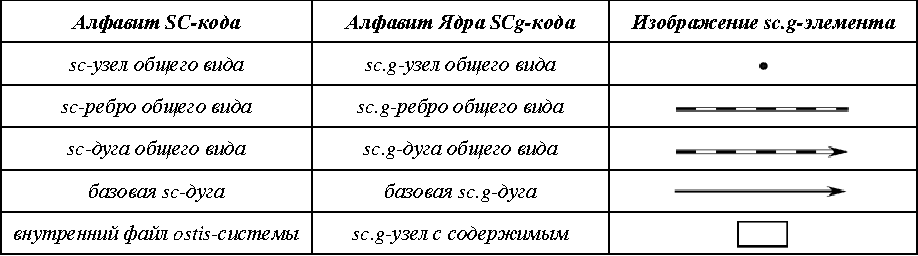
\includegraphics{figures/intro/scg/SCg-core-alphabet.pdf}}

%TODO сверить пропорции sc.g-элементов и изменить описание
\scnheader{sc.g-узел общего вида}
\scnidtf{\textit{sc.g-элемент}, являющийся графическим изображением \textit{sc-узла общего вида}}
\scnexplanation{Все \textit{sc-узлы}, не являющиеся знаками файлов, в тексте (конструкции) \textit{Ядра SCg-кода}, изображаются в виде небольших чёрных кругов одинакового диаметра, который обозначим через $\bm{d}$, и точная величина которого зависит от масштаба отображения \textit{sc.g-текста}.}

\scnheader{sc.g-ребро общего вида}
\scnidtf{\textit{sc.g-элемент}, являющийся графическим изображением \textit{sc-ребра общего вида}}
\scnexplanation{Каждое \textit{sc-ребро} в \textit{Ядре SCg-кода} изображается в виде широкой линии, в которой чередуются фрагменты со сплошной заливкой и без заливки, не имеющей самопересечений и имеющей общую толщину, равную примерно $\bm{0.7d}$.}

\scnheader{sc.g-дуга общего вида}
\scnidtf{\textit{sc.g-элемент}, являющийся графическим изображением \textit{sc-дуги общего вида}}
\scnexplanation{Каждая \textit{sc-дуга} в \textit{Ядре SCg-кода} изображается в виде широкой линии, в которой чередуются фрагменты со сплошной заливкой и без заливки, не имеющей самопересечений, имеющей общую толщину, равную примерно $\bm{0.7d}$ и имеющей изображение стрелочки на одном из концов этой линии.}

\scnheader{базовая sc.g-дуга}
\scnidtf{\textit{sc.g-элемент}, являющийся графическим изображением \textit{базовой sc-дуги}}
\scnexplanation{Каждая входящая в состав sc-текста \textit{базовая sc-дуга} в \textit{Ядре SCg-кода} изображается в виде линии произвольной формы, не имеющий самопересечений, имеющий толщину $\bm{0.4d}$, и имеющей изображение стрелочки на одном из ее концов.}

\scnheader{внутренний файл ostis-системы}
\scnidtf{sc-узел с содержимым}
\scnaddlevel{1}
\scniselement{часто используемый sc-идентификатор}
\scnaddlevel{-1}
\scnidtf{sc-узел, являющийся знаком внутреннего файла ostis-системы}
\scnidtf{sc-знак внутреннего файла ostis-системы}

\scnheader{sc.g-узел с содержимым}
\scnidtf{sc.g-узел, имеющий содержимое}
\scnidtf{sc.g-узел, являющийся знаком внутреннего файла ostis-системы}
\scnidtf{sc.g-знак внутреннего файла ostis-системы}
\scnidtf{sc.g-рамка, ограничивающая изображение (представление) внутреннего файла ostis-системы, обозначаемого этой sc.g-рамкой}
\scnidtf{sc.g-рамка}
\scnaddlevel{1}
\scnnote{\textit{sc.g-рамка} -- это всегда прямоугольник, максимальный размер которого не ограничивается, но минимальный фиксируется и соответствует \textit{sc.g-рамке}, внутри которой обозначаемый ею \textit{файл} не отображается.}
\scnaddlevel{-1}
\scnexplanation{Каждый входящий в sc-текст \textit{sc-узел, имеющий содержимое}, в \textit{Ядре SCg-кода} изображается в виде прямоугольника произвольного размера с толщиной линии $\bm{0.6d}$. Внутри этого прямоугольника отображается \textit{файл}, обозначаемый изображаемым \textit{sc-узлом}. Если нет необходимости изображать в тексте сам \textit{файл}, то \textit{sc-узел}, обозначающий такой \textit{файл}, в \textit{sc.g-тексте} изображается в виде прямоугольника со сторонами $\bm{2d}$ по вертикали и $\bm{4d}$ по горизонтали.}

\scnheader{Алфавит Ядра SCg-кода}
\scnnote{Трудно сразу поверить, что на основе такого простого алфавита можно построить удобный и \uline{универсальный} графовый язык. В рамках \textit{Документации Технологии OSTIS} мы постараемся Вас в этом убедить. Кроме того, нас не должна настораживать простота алфавита, поскольку человечество имеет большой опыт кодирования, хранения в памяти и передачи по каналам связи самых различных информационных ресурсов, используя алфавит, состоящий только из двух классов элементов -- единиц и нулей. 

Мы ведем речь о принципиально ином (графовом) способе кодирования информации в \textit{компьютерных системах}, но стараемся при этом свести это кодирование к достаточно простому алфавиту хотя бы для того, чтобы искусственно не усложнять проблему создания нового поколения компьютеров, основанных на указанном способе кодирования информации. 

Расширения \textit{Ядра SCg-кода} рассмотрим как направления перехода от текстов \textit{Ядра SCg-кода} к более компактным текстам. Но, поскольку это приводит к усложнению \textit{Синтаксиса SCg-кода} и, в первую очередь, к расширению \textit{Алфавита SCg-кода}, делать такие расширения необходимо обоснованно с учетом частоты встречаемости в рамках \textit{баз знаний ostis-систем} соответствующих фрагментов.}

\scnendstruct \scninlinesourcecommentpar{Завершили сегмент ``Описание Ядра SCg-кода''}

\scnsegmentheader{Описание Первого направления расширения Ядра SCg-кода}
\scnstartsubstruct

\bigskip
\scnheader{Первое направление расширения Ядра SCg-кода}

\scnexplanation{\textit{Первое направление синтаксического расширения Ядра SCg-кода} -- это \uline{приписывание} некоторым sc.g-элементам \textit{основных sc-идентификаторов*} (чаще всего - строковых идентификаторов, то есть имен) \textit{sc-элементов} , изображаемых этими \textit{sc.g-элементами}. Указываемые идентификаторы являются уникальным для каждого идентифицируемого (именуемого) \textit{sc.g-элемента}. Приписывание \textit{sc.g-элементам} уникальных идентификаторов дает возможность в рамках одного \textit{sc.g-текста} дублировать (копировать) некоторые \textit{sc.g-узлы} при условии, если \uline{всем} таким копиям будут приписаны соответствующие идентификаторы. Такое дублирование \textit{sc.g-узлов} является дополнительным средствам \uline{наглядного} размещения \textit{sc.g-текстов}. Кроме того, приписывание \textit{sc.g-элементу} соответствующего ему основного (уникального) \textit{sc-идентификатора*} представляет собой более компактный вариант изображения \textit{sc.g-текстов}.}

\scnheader{Пример sc.g-текста, трансформируемого по Первому направлению расширения Ядра SCg-кода}
\scneqscg{figures/intro/scg/scg_transf1.png}
\scniselement{sc.g-текст}
\scnexplanation{Здесь (в левом нижнем углу приведенного sc.g-текста) представлен \textit{sc.g-узел общего вида}, изображающий \textit{sc-узел общего вида}, которому соответствует \textit{основной sc-идентификатор*} в виде строки ``\textbf{\textit{ei}}''}
\scnrelfrom{трансформация sc.g-текста по Первому направлению расширения Ядра SCg-кода}{\scnfilescg{figures/intro/scg/scg_transf2.png}}
\scnaddlevel{1}
    \scniselement{sc.g-текст}
    \scnexplanation{\textit{sc.g-узлу общего вида} изображающему \textit{sc-узел}, внешним идентификатором которого является строка ``\textit{основной sc-идентификатор*}'' и который, соответственно является знаком \textit{бинарного ориентированного отношения}, каждая \textit{пара} которого связывает идентифицируемый \textit{sc-элемент} с его основным внешним sc-идентификатором, приписывается указанный внешний идентификатор изображаемого им \textit{sc-элемента}.}
    \scnrelfrom{трансформация sc.g-текста по Первому направлению расширения Ядра SCg-кода}{\scnfilescg{figures/intro/scg/scg_transf3.png}}
    \scnaddlevel{1}
        \scniselement{sc.g-текст} 
        \scnexplanation{В результате данной трансформации исходный \textit{sc.g-текст} трансформируется в один \textit{sc.g-общего вида}, которому приписывается \textit{основной sc-идентификатор} ``\textit{\textbf{ei}}''.}
    \scnaddlevel{-1}
\scnaddlevel{-1}


\scnheader{трансформация sc.g-текста по Первому направлению расширения Ядра SCg-кода*}
\scnidtf{Бинарное ориентированное отношение, каждая пара которого связывает исходный вид трансформируемого sc.g-текста и результат этой трансформации}
\scnnote{Подчеркнем, что рассматриваемая трансформация преобразует исходный текст Ядра \textit{SCg-кода} в текст, семантически эквивалентный, но принадлежащий не Ядру \textit{SCg-кода}, а его расширению.
}

\scnheader{синтаксическая трансформация*}
\scnidtf{синтаксическая трансформация информационной конструкции*}
\scnsuperset{синтаксическая трансформация sc.g-текста*}
\scnaddlevel{1}
\scnsuperset{трансформация sc.g-текста по Первому направлению расширения Ядра SCg-кода*}
\scnaddlevel{-1}

\scnendstruct \scninlinesourcecommentpar{Завершили сегмент "Описание первого направления расширения Ядра SCg-кода}
\bigskip

\scnsegmentheader{Описание Второго направления расширения Ядра SCg-кода}
\scnstartsubstruct

\scnheader{Второе направление расширения Ядра SCg-кода}
\scnexplanation{\textit{Второе направление расширения Ядра SCg-кода} -- это уточнение типологии \textit{константных постоянных сущностей} и расширение \textit{Алфавита Ядра SCg-кода}, позволяющее типологию \textit{константных постоянных сущностей} привести в соответствие с синтаксической типологией новых вводимых элементов \textit{Алфавита SCg-кода}. Рассмотрим подробнее sc.g-элементы, знаки \textit{константных постоянных сущностей} различного вида. Графическим признаком \textit{константных постоянных sc-узлов} в конструкциях SCg-кода является их изображение в виде \uline{окружностей} диаметра $3d$, где $d$ -- диаметр sc.g-узла общего вида. Такое изображение является более компактной записью факта принадлежности заданного sc-узла (назовем его $\bm{vi}$) классу sc-констант и классу обозначений постоянных сущностей. Запись этого факта в \textit{Ядре SCg-кода} потребует (1) явного изображения sc-узла, обозначающего класс всевозможных константных sc-элементов (класс \textit{sc-констант}), (2) явного изображения базовой sc-дуги, соединяющего изображение sc-узла, обозначающего класс sc-констант, с изображением заданного константного sc-узла, (3) явного изображение sc-узла, обозначающего класс всевозможных sc-элементов, обозначающих \textit{постоянные сущности}, (4) явного изображения базовой sc-дуги, соединяющего изображение sc-узла, обозначающего класс обозначений \textit{постоянных сущностей} с изображением рассматриваемого sc-узла $\bm{vi}$ (Смотрите \textit{Файл. Изображение спецификации sc.g-элемента средствами Ядра SCg-кода и Первого расширения Ядра SCg-кода}).

Общепринятая запись данного факта выглядит следующим образом:

``\textit{sc-константа} $\ni \bm{vi}$; \textit{постоянная сущность} $\ni \bm{v_i};$''

\textit{Константные постоянные sc-ребра} в конструкциях SCg-кода изображаются в виде двойной линии, каждая из которых имеет толщину примерно $d/7$, а расстояние между ними равно примерно $3d/7$. 

\textit{Константные постоянные sc-дуги} изображаются в виде такой же двойной линии, но со стрелочкой. Все \textit{базовые sc-дуги}, а также все sc-узлы, имеющие содержимое, по определению являются \textit{константными постоянными sc-элементами}. 

\textit{Константные sc.g-узлы}, изображаемые окружностями диаметра $3d$ и толщиной границы $d/5$, обозначают \textit{константные постоянные сущности}, о которых мало что известно, но известно то, что они не являются парами (то есть множествами, \textit{мощность*} которых равна 2) и, следовательно, не могут быть изображёны в виде sc.g-дуг или sc.g-рёбер. Но, если при этом об обозначаемой \textit{константной постоянной сущности} ($\bm{vi}$) известно, что она является классом сущностей, то явное указание принадлежности sc-элемента \textit{vi} всевозможных классов можно заменить на специальное графическое изображение sc-элемента \textit{vi}, предполагаемое указанную принадлежность. Это приводит к расширению  \textit{Алфавита SCg-кода} (см. \textit{Примеры sc.g-текстов, трансформируемых по Второму направлению расширения Ядра SCg-код}).

Аналогичным образом (см. \textit{Примеры sc.g-текстов, трансформируемых по Второму направлению расширения Ядра SCg-код}) вводятся: 
\begin{scnitemize}
\item sc.g-узел, являющийся изображением \textit{класса};  
\item sc.g-узел, являющийся изображением \textit{класса классов};  
\item sc.g-узел, являющийся изображением \textit{отношения}; 
\item sc.g-узел, являющийся изображением \textit{ролевого отношения}; 
\item sc.g-узел, являющийся изображением \textit{sc-структуры};  
\item sc.g-узел, являющийся изображением \textit{небинарной sc-связки};
\item sc.g-узел, являющийся изображением \textit{первичной сущности} (терминальной сущности, которая не является множеством, а также файлом, хранимым в памяти ostis-системы).
\end{scnitemize}

Важное место среди константных постоянных сущностей занимают \textit{константные постоянные пары принадлежности}, обозначаемое соответствующими \textit{sc.g-дугами}. Такие пары принадлежности и обозначающие их sc.g-дуги бывают позитивными, негативными и нечеткими. Константная постоянная позитивная sc.g-дуга принадлежности есть ничто иное, как \textit{базовая sc.g-дуга}. Константная постоянная негативная sc.g-дуга принадлежности изображается в виде \textit{базовой sc.g-дуги}, перечеркнутой штриховыми черточками. Константная постоянная нечёткая sc.g-дуга принадлежности изображается в виде "недочеркнутой"{} \textit{базовой sc.g-дуги}, с каждой стороны которой отображаются штрихи, по длине равные половине от длины штрихов, которыми перечеркнута \textit{константная постоянная негативная sc.g-дуга}.}

\scnheader{Файл. Изображение спецификации sc.g-элемента средствами Ядра SCg-кода и Второго направления расширения Ядра SCg-кода}
\scneqscg{figures/intro/scg/scg2ex.png}

\scnheader{Примеры sc.g-текстов, трансформируемых по Второму направлению расширения Ядра SCg-кода}
\scnstructinclusion

\scnmakeset{\scgfileitem{figures/intro/scg/scg2_ex1.png}\\
\scnaddlevel{1}
    \scnrelfrom{синтаксическая трансформация}{\scnfilescg{figures/intro/scg/scg2_ex1_1.png}}
    \scnaddlevel{1}
        \scnexplanation{Здесь вводится новый синтаксический вид \textit{sc.g-элементов} -- \textit{константный постоянный sc.g-узел общего вида}, изображаемый окружностью диаметра $3d$ и толщиной границы $d/5$.}
    \scnaddlevel{-1}
\scnaddlevel{-1};
\scgfileitem{figures/intro/scg/nodes/const_perm/sc.g_const_perm_class1.png}\\
\scnaddlevel{1}
    \scnrelfrom{синтаксическая трансформация}{\scnfilescg{figures/intro/scg/nodes/const_perm/sc.g_const_perm_class2.png}}
    \scnaddlevel{1}
        \scnexplanation{Здесь вводится новый синтаксический вид \textit{sc.g-элементов} -- \textit{константный постоянный sc.g-узел, обозначающий класс}, изображаемый как \textit{константный постоянный sc.g-узел} с "решеткой"{} внутри.}
    \scnaddlevel{-1}
\scnaddlevel{-1};
\scgfileitem{figures/intro/scg/nodes/const_perm/sc.g_const_perm_class_of_classes1.png}\\
\scnaddlevel{1}
    \scnrelfrom{синтаксическая трансформация}{\scnfilescg{figures/intro/scg/nodes/const_perm/sc.g_const_perm_class_of_classes2.png}}
    \scnaddlevel{1}
        \scnexplanation{Здесь вводится новый синтаксический вид \textit{sc.g-элементов} -- \textit{константный постоянный sc.g-узел, обозначающий класс классов}, изображаемый как \textit{константный постоянный sc.g-узел} с направленным вверх углом внутри.}
    \scnaddlevel{-1}
\scnaddlevel{-1};
\scgfileitem{figures/intro/scg/nodes/const_perm/sc.g_const_perm_norole1.png}\\
\scnaddlevel{1}
    \scnrelfrom{синтаксическая трансформация}{\scnfilescg{figures/intro/scg/nodes/const_perm/sc.g_const_perm_norole2.png}}
    \scnaddlevel{1}
        \scnexplanation{Здесь вводится новый синтаксический вид \textit{sc.g-элементов} -- \textit{константный постоянный sc.g-узел, обозначающий неролевое отношение}, изображаемый как \textit{константный постоянный sc.g-узел} с "крестиком"{} внутри.}
    \scnaddlevel{-1}
\scnaddlevel{-1};
\scgfileitem{figures/intro/scg/nodes/const_perm/sc.g_const_perm_role1.png}\\
\scnaddlevel{1}
    \scnrelfrom{синтаксическая трансформация}{\scnfilescg{figures/intro/scg/nodes/const_perm/sc.g_const_perm_role2.png}}
    \scnaddlevel{1}
        \scnexplanation{Здесь вводится новый синтаксический вид \textit{sc.g-элементов} -- \textit{константный постоянный sc.g-узел, обозначающий ролевое отношение}, изображаемый как \textit{константный постоянный sc.g-узел} с "плюсом"{} внутри.}
    \scnaddlevel{-1}
\scnaddlevel{-1};
\scgfileitem{figures/intro/scg/nodes/const_perm/sc.g_const_perm_structure1.png}\\
\scnaddlevel{1}
    \scnrelfrom{синтаксическая трансформация}{\scnfilescg{figures/intro/scg/nodes/const_perm/sc.g_const_perm_structure2.png}}
    \scnaddlevel{1}
        \scnexplanation{Здесь вводится новый синтаксический вид \textit{sc.g-элементов} -- \textit{константный постоянный sc.g-узел, обозначающий sc-структуру}, изображаемый как \textit{константный постоянный sc.g-узел} с точкой внутри.}
    \scnaddlevel{-1}
\scnaddlevel{-1};
\scgfileitem{figures/intro/scg/nodes/const_perm/sc.g_const_perm_primary_entity1.png}\\
\scnaddlevel{1}
    \scnrelfrom{синтаксическая трансформация}{\scnfilescg{figures/intro/scg/nodes/const_perm/sc.g_const_perm_primary_entity2.png}}
    \scnaddlevel{1}
        \scnexplanation{Здесь вводится новый синтаксический вид \textit{sc.g-элементов} -- \textit{константный постоянный sc.g-узел, обозначающий первичную сущность}, изображаемый как \textit{константный постоянный sc.g-узел} с  косой штриховкой внутри.}
    \scnaddlevel{-1}
\scnaddlevel{-1};
\scgfileitem{figures/intro/scg/nodes/const_perm/sc.g_const_perm_tuple1.png}\\
\scnaddlevel{1}
    \scnrelfrom{синтаксическая трансформация}{\scnfilescg{figures/intro/scg/nodes/const_perm/sc.g_const_perm_tuple2.png}}
    \scnaddlevel{1}
        \scnexplanation{Здесь вводится новый синтаксический вид \textit{sc.g-элементов} -- \textit{константный постоянный sc.g-узел, обозначающий небинарную sc-связку}, изображаемый как \textit{константный постоянный sc.g-узел} с горизонтальной линией внутри.}
    \scnaddlevel{-1}
\scnaddlevel{-1};
\scgfileitem{figures/intro/scg/arcs/const/scg_const_perm_noorien1.png}\\
\scnaddlevel{1}
    \scnrelfrom{синтаксическая трансформация}{\scnfilescg{figures/intro/scg/arcs/const/scg_const_perm_noorien2.png}}
    \scnaddlevel{1}
        \scnexplanation{Здесь вводится новый синтаксический вид \textit{sc.g-элементов} -- \textit{константное постоянное sc.g-ребро}, изображаемое двумя непрерывными параллельными линиями.}
    \scnaddlevel{-1}
\scnaddlevel{-1};
\scgfileitem{figures/intro/scg/arcs/const/scg_const_perm_orient1.png}\\
\scnaddlevel{1}
    \scnrelfrom{синтаксическая трансформация}{\scnfilescg{figures/intro/scg/arcs/const/scg_const_perm_orient2.png}}
    \scnaddlevel{1}
        \scnexplanation{Здесь вводится новый синтаксический вид \textit{sc.g-элементов} -- \textit{константная постоянная sc.g-дуга}, изображаемая двумя непрерывными параллельными линиями с общей стрелкой на одном из концов.}
    \scnaddlevel{-1}
\scnaddlevel{-1};
\scgfileitem{figures/intro/scg/arcs/const/scg_const_perm_positive1.png}\\
\scnaddlevel{1}
    \scnrelfrom{синтаксическая трансформация}{\scnfilescg{figures/intro/scg/arcs/const/scg_const_perm_positive2.png}}
    \scnaddlevel{1}
        \scnexplanation{\textit{Константная постоянная позитивная sc.g-дуга принадлежности} есть ничто иное, как \textit{базовая sc.g-дуга}.}
    \scnaddlevel{-1}
\scnaddlevel{-1};
\scgfileitem{figures/intro/scg/arcs/const/scg_const_perm_negative1.png}\\
\scnaddlevel{1}
    \scnrelfrom{синтаксическая трансформация}{\scnfilescg{figures/intro/scg/arcs/const/scg_const_perm_negative2.png}}
    \scnaddlevel{1}
        \scnexplanation{Здесь вводится новый синтаксический вид \textit{sc.g-элементов} -- \textit{константная постоянная негативная sc.g-дуга принадлежности}, изображается в виде \textit{базовой sc.g-дуги}, перечеркнутой штриховыми черточками.}
    \scnaddlevel{-1}
\scnaddlevel{-1};
\scgfileitem{figures/intro/scg/arcs/const/scg_const_perm_fuzzy1.png}\\
\scnaddlevel{1}
    \scnrelfrom{синтаксическая трансформация}{\scnfilescg{figures/intro/scg/arcs/const/scg_const_perm_fuzzy2.png}}
    \scnaddlevel{1}
        \scnexplanation{Здесь вводится новый синтаксический вид \textit{sc.g-элементов} -- \textit{константная постоянная нечеткая sc.g-дуга принадлежности}, которая изображается в виде "недочеркнутой"{} \textit{базовой sc.g-дуги}, с каждой стороны которой отображаются штрихи, по длине равные половине от длины штрихов, которыми перечеркнута \textit{константная постоянная негативная sc.g-дуга}.}
    \scnaddlevel{-1}
\scnaddlevel{-1}
}

\scnheader{Примеры sc.g-текста, записанного средствами Второго направления расширения Ядра SCg-кода}
\scnstructinclusion

\scnmakeset{\scgfileitem{figures/intro/scg/examples/scg_example_triangle.png}
\scnaddlevel{1}
\scniselementrole{пример}{sc.g-текст}
\scnexplanation{Данный sc.g-текст содержит следующую информацию:
\begin{scnitemize}
\item Сущности \textit{Треугольник ABC}~~ и ~~\textit{Треугольник CDE} являются треугольниками (принадлежат классу \textit{треугольников}). При этом известно, что площадь \textit{Треугольника CDE} в 4 раза больше, чем площадь \textit{Треугольника ABC}, но конкретные значения ллощадей не известны\char59
\item Сущность \textit{Отрезок DE} является отрезком (принадлежит классу \textit{отрезков}) и является стороной \textit{Треугольника CDE}. Кроме того, у \textit{Отрезка DE} есть длина, измерение которой в сантиметрах составляет 5. Обратите внимание, что в данном случае для упрощения понимания использовано бинарное отношение \textit{длина*}, которое является \textit{неосновным понятием} и в базе знаний заменяется на \textit{базовую sc-дугу}, связывающую величину как класс эквивалентности с конкретной сущностью, входящей в данный класс, в данном случае -- \textit{Отрезок DE}\char59  
\item Сущность \textit{Треугольник AEB} является треугольником и имеет \textit{внутренний угол*}~~~ \textit{Угол AEB}. В свою очередь, \textit{Угол AEB} является \textit{углом} и имеет \textit{косинус*}, равный 0,5\char59
\item \textit{Треугольник AEB} имеет \textit{сторону*} (не указывается, какая именно из сторон имеется в виду), \textit{средней точкой*} которой является \textit{Точка O}. В свою очередь, \textit{Точка O} является центром некоторой \textit{Окружности O}, которая относится к классу \textit{окружностей}.
\end{scnitemize}
}\scnaddlevel{-1};
\scgfileitem{figures/intro/scg/examples/scg_example_alice.png}
\scnaddlevel{1}
	\scnnote{Данный sc.g-текст основан на популярном примере, наглядно иллюстрируещем понятие семантической сети, известном как ``Социальная сеть Алисы''. Как видно из примера, данный текст описывает различные взаимосвязи персоны по имени Алиса, при этом некоторые из используемых отношений является ориентированными (например, ``работник*''), а некоторые -- неориентированными (например, ``друг*'').}
\scnaddlevel{-1}
}

\scnendstruct

\scnsegmentheader{Описание Третьего направления расширения Ядра SCg-кода}

\scnstartsubstruct

\bigskip
\scnfilelong{\textit{Третье направление расширения Ядра SCg-кода} -- это расширение его алфавита путем введения дополнительных sc.g-элементов, обозначающих \textit{константные временные сущности} различного вида. Признаком sc.g-элементов, обозначающих \textit{константные временные сущности} являются точечные линии (линии, состоящие из точек, размер которых равен размеру изображаемой линии и которые близко расположены друг к другу на расстоянии, равном половине их размера), с помощью которых рисуются окружности при изображении sc-узлов, а также линии при изображении sc-коннекторов.

Результатом \textit{Третьего направления расширения Ядра SCg-кода} является введение следующих видов sc.g-элементов (см. \textit{Примеры sc.g-текстов, трансформируемых по Третьему направлению расширения Ядра SCg-кода}).}

\scnheader{Примеры sc.g-текстов, трансформируемых по Третьему направлению расширения Ядра SCg-кода}
\scnstructinclusion
\scnmakeset{\scgfileitem{figures/intro/scg/nodes/const_temp/sc.g_const_temp_general_view1.png}\\
\scnaddlevel{1}
    \scnrelfrom{синтаксическая трансформация}{\scnfilescg{figures/intro/scg/nodes/const_temp/sc.g_const_temp_general_view2.png}}
    \scnaddlevel{1}
        \scnexplanation{Здесь вводится новый синтаксический вид \textit{sc.g-элементов} -- \textit{константный временный sc.g-узел общего вида}, изображаемый точечной окружностью диаметра $3d$ и толщиной границы $d/5$.}
    \scnaddlevel{-1}
\scnaddlevel{-1};
\scgfileitem{figures/intro/scg/nodes/const_temp/sc.g_const_temp_class1.png}\\
\scnaddlevel{1}
    \scnrelfrom{синтаксическая трансформация}{\scnfilescg{figures/intro/scg/nodes/const_temp/sc.g_const_temp_class2.png}}
    \scnaddlevel{1}
        \scnexplanation{Здесь вводится новый синтаксический вид \textit{sc.g-элементов} -- \textit{константный временный sc.g-узел, обозначающий класс}, изображаемый как \textit{константный временный sc.g-узел} с "решеткой"{} внутри.}
    \scnaddlevel{-1}
\scnaddlevel{-1};
\scgfileitem{figures/intro/scg/nodes/const_temp/sc.g_const_temp_class_of_classes1.png}\\
\scnaddlevel{1}
    \scnrelfrom{синтаксическая трансформация}{\scnfilescg{figures/intro/scg/nodes/const_temp/sc.g_const_temp_class_of_classes2.png}}
    \scnaddlevel{1}
        \scnexplanation{Здесь вводится новый синтаксический вид \textit{sc.g-элементов} -- \textit{константный временный sc.g-узел, обозначающий класс классов}, изображаемый как \textit{константный временный sc.g-узел} с направленным вверх углом внутри.}
    \scnaddlevel{-1}
\scnaddlevel{-1};
\scgfileitem{figures/intro/scg/nodes/const_temp/sc.g_const_temp_norole1.png}\\
\scnaddlevel{1}
    \scnrelfrom{синтаксическая трансформация}{\scnfilescg{figures/intro/scg/nodes/const_temp/sc.g_const_temp_norole2.png}}
    \scnaddlevel{1}
        \scnexplanation{Здесь вводится новый синтаксический вид \textit{sc.g-элементов} -- \textit{константный временный sc.g-узел, обозначающий неролевое отношение}, изображаемый как \textit{константный временный sc.g-узел} с "крестиком"{} внутри.}
    \scnaddlevel{-1}
\scnaddlevel{-1};
\scgfileitem{figures/intro/scg/nodes/const_temp/sc.g_const_temp_role1.png}\\
\scnaddlevel{1}
    \scnrelfrom{синтаксическая трансформация}{\scnfilescg{figures/intro/scg/nodes/const_temp/sc.g_const_temp_role2.png}}
    \scnaddlevel{1}
        \scnexplanation{Здесь вводится новый синтаксический вид \textit{sc.g-элементов} -- \textit{константный временный sc.g-узел, обозначающий ролевое отношение}, изображаемый как \textit{константный временный sc.g-узел} с "плюсом"{} внутри.}
    \scnaddlevel{-1}
\scnaddlevel{-1};
\scgfileitem{figures/intro/scg/nodes/const_temp/sc.g_const_temp_structure1.png}\\
\scnaddlevel{1}
    \scnrelfrom{синтаксическая трансформация}{\scnfilescg{figures/intro/scg/nodes/const_temp/sc.g_const_temp_structure2.png}}
    \scnaddlevel{1}
        \scnexplanation{Здесь вводится новый синтаксический вид \textit{sc.g-элементов} -- \textit{константный временный sc.g-узел, обозначающий sc-структуру}, изображаемый как \textit{константный временный sc.g-узел} с точкой внутри.}
    \scnaddlevel{-1}
\scnaddlevel{-1};
\scgfileitem{figures/intro/scg/nodes/const_temp/sc.g_const_temp_primary_entity1.png}\\
\scnaddlevel{1}
    \scnrelfrom{синтаксическая трансформация}{\scnfilescg{figures/intro/scg/nodes/const_temp/sc.g_const_temp_primary_entity2.png}}
    \scnaddlevel{1}
        \scnexplanation{Здесь вводится новый синтаксический вид \textit{sc.g-элементов} -- \textit{константный временный sc.g-узел, обозначающий первичную сущность}, изображаемый как \textit{константный временный sc.g-узел} с  косой штриховкой внутри.}
    \scnaddlevel{-1}
\scnaddlevel{-1};
\scgfileitem{figures/intro/scg/nodes/const_temp/sc.g_const_temp_tuple1.png}\\
\scnaddlevel{1}
    \scnrelfrom{синтаксическая трансформация}{\scnfilescg{figures/intro/scg/nodes/const_temp/sc.g_const_temp_tuple2.png}}
    \scnaddlevel{1}
        \scnexplanation{Здесь вводится новый синтаксический вид \textit{sc.g-элементов} -- \textit{константный временный sc.g-узел, обозначающий небинарную sc-связку}, изображаемый как \textit{константный временный sc.g-узел} с горизонтальной линией внутри.}
    \scnaddlevel{-1}
\scnaddlevel{-1};
\scgfileitem{figures/intro/scg/arcs/const/scg_const_temp_noorien1.png}\\
\scnaddlevel{1}
    \scnrelfrom{синтаксическая трансформация}{\scnfilescg{figures/intro/scg/arcs/const/scg_const_temp_noorien2.png}}
    \scnaddlevel{1}
        \scnexplanation{Здесь вводится новый синтаксический вид \textit{sc.g-элементов} -- \textit{константное временное sc.g-ребро}, изображаемое двумя точечными параллельными линиями.}
    \scnaddlevel{-1}
\scnaddlevel{-1};
\scgfileitem{figures/intro/scg/arcs/const/scg_const_temp_orient1.png}\\
\scnaddlevel{1}
    \scnrelfrom{синтаксическая трансформация}{\scnfilescg{figures/intro/scg/arcs/const/scg_const_temp_orient2.png}}
    \scnaddlevel{1}
        \scnexplanation{Здесь вводится новый синтаксический вид \textit{sc.g-элементов} -- \textit{константная временная sc.g-дуга}, изображаемая двумя точечными параллельными линиями с общей стрелкой на одном из концов.}
    \scnaddlevel{-1}
\scnaddlevel{-1};
\scgfileitem{figures/intro/scg/arcs/const/scg_const_temp_positive1.png}\\
\scnaddlevel{1}
    \scnrelfrom{синтаксическая трансформация}{\scnfilescg{figures/intro/scg/arcs/const/scg_const_temp_positive2.png}}
    \scnaddlevel{1}
        \scnexplanation{Здесь вводится новый синтаксический вид \textit{sc.g-элементов} -- \textit{константная временная позитивная sc.g-дуга принадлежности}, изображаемая точечной линией со стрелкой на конце.}
    \scnaddlevel{-1}
\scnaddlevel{-1};
\scgfileitem{figures/intro/scg/arcs/const/scg_const_temp_negative1.png}\\
\scnaddlevel{1}
    \scnrelfrom{синтаксическая трансформация}{\scnfilescg{figures/intro/scg/arcs/const/scg_const_temp_negative2.png}}
    \scnaddlevel{1}
        \scnexplanation{Здесь вводится новый синтаксический вид \textit{sc.g-элементов} -- \textit{константная временная негативная sc.g-дуга принадлежности}, изображаемая точечной линией, перечеркнутой штриховыми черточками, со стрелкой на конце.}
    \scnaddlevel{-1}
\scnaddlevel{-1};
\scgfileitem{figures/intro/scg/arcs/const/scg_const_temp_fuzzy1.png}\\
\scnaddlevel{1}
    \scnrelfrom{синтаксическая трансформация}{\scnfilescg{figures/intro/scg/arcs/const/scg_const_temp_fuzzy2.png}}
    \scnaddlevel{1}
        \scnexplanation{Здесь вводится новый синтаксический вид \textit{sc.g-элементов} -- \textit{константная временная нечеткая sc.g-дуга принадлежности}, которая изображается в виде "недочеркнутой"{} \textit{\textit{константной временной позитивная sc.g-дуги принадлежности}, с каждой стороны которой отображаются штрихи, по длине равные половине от длины штрихов, которыми перечеркнута \textit{константная постоянная негативная sc.g-дуга}.}
    \scnaddlevel{-1}
\scnaddlevel{-1}
}
}

\scnendstruct

\scnsegmentheader{Описание Четвёртого направления расширения Ядра SCg-кода}

\scnstartsubstruct

\bigskip
\scnfilelong{Четвёртое направление расширения \textit{Ядра SCg-кода} -- это расширение его алфавита путем введения дополнительных элементов, обозначающих \textit{переменные постоянные сущности} различного вида. Признаком sc.g-элементов, обозначающих сущности указанного класса, являются квадратики для изображения обозначений \textit{переменных постоянных сущностей}, не являющихся бинарными связями, а также пунктирные и штрих-пунктирные линии для изображения \textit{переменных постоянных бинарных связей}. 

Подчеркнем, что \textit{переменные постоянные сущности} могут отличаться друг от друга по характеру их \textit{области значений*}. Этими значениями в общем случае могут быть как \textit{константные постоянные сущности}, так и \textit{переменные постоянные сущности}. В любом случае, значение \textit{переменной сущности} является либо \textit{константной сущностью}, либо \textit{переменной сущностью}. Если каждое значение переменной является константой, то такую переменную будем называть \textit{переменной первого уровня}. Если каждое значение переменной является \textit{переменной первого уровня}, то такую переменную будем называть \textit{переменной второго уровня}. 

\textit{Переменная постоянная сущность первого уровня } (первичная sc-переменная), не являющаяся бинарной связью -- это переменная, каждым значением которой является \textit{константная постоянная сущность}, не являющаяся бинарной связью. Такая переменная изображается квадратиком, который ориентирован по вертикали и горизонтали. 

\textit{переменная постоянная сущность второго уровня} (вторичная sc-переменная), не являющаяся бинарной связью, изображается квадратиком, повернутым на 45$^\circ$. 

Указанная выше семантика таких изображений приписывается \uline{по умолчанию}. Это означает, что, если обозначаемая sc-переменная имеет более сложную структуру области её значений (является sc-переменной третьего и выше уровня или sc-переменной, значения которой имеют различный логический уровень), то эта область должна быть специфицирована явно, при этом такая sc-переменная в SCg-коде изображается так же, как первичная sc-переменная.}

\scnheader{Примеры sc.g-текстов, трансформируемых по Четвертому направлению расширения Ядра SCg-кода}
\scnstructinclusion
\scnmakeset{\scgfileitem{figures/intro/scg/nodes/var_perm/sc.g_var_perm_general_view1.png}\\
\scnaddlevel{1}
    \scnrelfrom{синтаксическая трансформация}{\scnfilescg{figures/intro/scg/nodes/var_perm/sc.g_var_perm_general_view2.png}}
    \scnaddlevel{1}
        \scnexplanation{Здесь вводится новый синтаксический вид \textit{sc.g-элементов} -- \textit{переменный постоянный sc.g-узел общего вида}, изображаемый квадратиком cj со стороной длины $3d$ и толщиной границы $d/5$.}
    \scnaddlevel{-1}
\scnaddlevel{-1};
\scgfileitem{figures/intro/scg/nodes/var_perm/sc.g_var_perm_class1.png}\\
\scnaddlevel{1}
    \scnrelfrom{синтаксическая трансформация}{\scnfilescg{figures/intro/scg/nodes/var_perm/sc.g_var_perm_class2.png}}
    \scnaddlevel{1}
        \scnexplanation{Здесь вводится новый синтаксический вид \textit{sc.g-элементов} -- \textit{переменный постоянный sc.g-узел, обозначающий класс}, изображаемый как \textit{переменный постоянный sc.g-узел} с "решеткой"{} внутри.}
    \scnaddlevel{-1}
\scnaddlevel{-1};
\scgfileitem{figures/intro/scg/nodes/var_perm/sc.g_var_perm_class_of_classes1.png}\\
\scnaddlevel{1}
    \scnrelfrom{синтаксическая трансформация}{\scnfilescg{figures/intro/scg/nodes/var_perm/sc.g_var_perm_class_of_classes2.png}}
    \scnaddlevel{1}
        \scnexplanation{Здесь вводится новый синтаксический вид \textit{sc.g-элементов} -- \textit{переменный постоянный sc.g-узел, обозначающий класс классов}, изображаемый как \textit{переменный постоянный sc.g-узел} с направленным вверх углом внутри.}
    \scnaddlevel{-1}
\scnaddlevel{-1};
\scgfileitem{figures/intro/scg/nodes/var_perm/sc.g_var_perm_norole1.png}\\
\scnaddlevel{1}
    \scnrelfrom{синтаксическая трансформация}{\scnfilescg{figures/intro/scg/nodes/var_perm/sc.g_var_perm_norole2.png}}
    \scnaddlevel{1}
        \scnexplanation{Здесь вводится новый синтаксический вид \textit{sc.g-элементов} -- \textit{переменный постоянный sc.g-узел, обозначающий неролевое отношение}, изображаемый как \textit{переменный постоянный sc.g-узел} с "крестиком"{} внутри.}
    \scnaddlevel{-1}
\scnaddlevel{-1};
\scgfileitem{figures/intro/scg/nodes/var_perm/sc.g_var_perm_role1.png}\\
\scnaddlevel{1}
    \scnrelfrom{синтаксическая трансформация}{\scnfilescg{figures/intro/scg/nodes/var_perm/sc.g_var_perm_role2.png}}
    \scnaddlevel{1}
        \scnexplanation{Здесь вводится новый синтаксический вид \textit{sc.g-элементов} -- \textit{переменный постоянный sc.g-узел, обозначающий ролевое отношение}, изображаемый как \textit{переменный постоянный sc.g-узел} с "плюсом"{} внутри..}
    \scnaddlevel{-1}
\scnaddlevel{-1};
\scgfileitem{figures/intro/scg/nodes/var_perm/sc.g_var_perm_structure1.png}\\
\scnaddlevel{1}
    \scnrelfrom{синтаксическая трансформация}{\scnfilescg{figures/intro/scg/nodes/var_perm/sc.g_var_perm_structure2.png}}
    \scnaddlevel{1}
        \scnexplanation{Здесь вводится новый синтаксический вид \textit{sc.g-элементов} -- \textit{переменный постоянный sc.g-узел, обозначающий sc-структуру}, изображаемый как \textit{переменный постоянный sc.g-узел} с точкой внутри.}
    \scnaddlevel{-1}
\scnaddlevel{-1};
\scgfileitem{figures/intro/scg/nodes/var_perm/sc.g_var_perm_primary_entity1.png}\\
\scnaddlevel{1}
    \scnrelfrom{синтаксическая трансформация}{\scnfilescg{figures/intro/scg/nodes/var_perm/sc.g_var_perm_primary_entity2.png}}
    \scnaddlevel{1}
        \scnexplanation{Здесь вводится новый синтаксический вид \textit{sc.g-элементов} -- \textit{переменный постоянный sc.g-узел, обозначающий первичную сущность}, изображаемый как \textit{переменный постоянный sc.g-узел} с  косой штриховкой внутри.}
    \scnaddlevel{-1}
\scnaddlevel{-1};
\scgfileitem{figures/intro/scg/nodes/var_perm/sc.g_var_perm_tuple1.png}\\
\scnaddlevel{1}
    \scnrelfrom{синтаксическая трансформация}{\scnfilescg{figures/intro/scg/nodes/var_perm/sc.g_var_perm_tuple2.png}}
    \scnaddlevel{1}
        \scnexplanation{Здесь вводится новый синтаксический вид \textit{sc.g-элементов} -- \textit{переменный постоянный sc.g-узел, обозначающий небинарную sc-связку}, изображаемый как \textit{переменный постоянный sc.g-узел} с горизонтальной линией внутри.}
    \scnaddlevel{-1}
\scnaddlevel{-1};
\scgfileitem{figures/intro/scg/arcs/var/scg_var_perm_noorien1.png}\\
\scnaddlevel{1}
    \scnrelfrom{синтаксическая трансформация}{\scnfilescg{figures/intro/scg/arcs/var/scg_var_perm_noorien2.png}}
    \scnaddlevel{1}
        \scnexplanation{Здесь вводится новый синтаксический вид \textit{sc.g-элементов} -- \textit{переменное постоянное sc.g-ребро}, изображаемое двумя пунктирными параллельными линиями.}
    \scnaddlevel{-1}
\scnaddlevel{-1};
\scgfileitem{figures/intro/scg/arcs/var/scg_var_perm_orient1.png}\\
\scnaddlevel{1}
    \scnrelfrom{синтаксическая трансформация}{\scnfilescg{figures/intro/scg/arcs/var/scg_var_perm_orient2.png}}
    \scnaddlevel{1}
        \scnexplanation{Здесь вводится новый синтаксический вид \textit{sc.g-элементов} -- \textit{переменная постоянная sc.g-дуга}, изображаемая двумя пунктирными параллельными линиями с общей стрелкой на одном из концов.}
    \scnaddlevel{-1}
\scnaddlevel{-1};
\scgfileitem{figures/intro/scg/arcs/var/scg_var_perm_positive1.png}\\
\scnaddlevel{1}
    \scnrelfrom{синтаксическая трансформация}{\scnfilescg{figures/intro/scg/arcs/var/scg_var_perm_positive2.png}}
    \scnaddlevel{1}
        \scnexplanation{\textit{переменная постоянная позитивная sc.g-дуга принадлежности}, изображаемая пунктирной линией со стрелкой на конце.}
    \scnaddlevel{-1}
\scnaddlevel{-1};
\scgfileitem{figures/intro/scg/arcs/var/scg_var_perm_negative1.png}\\
\scnaddlevel{1}
    \scnrelfrom{синтаксическая трансформация}{\scnfilescg{figures/intro/scg/arcs/var/scg_var_perm_negative2.png}}
    \scnaddlevel{1}
        \scnexplanation{Здесь вводится новый синтаксический вид \textit{sc.g-элементов} -- \textit{переменная постоянная негативная sc.g-дуга принадлежности}, изображается в виде \textit{переменной постоянной позитивной sc.g-дуги принадлежности}, перечеркнутой штриховыми черточками.}
    \scnaddlevel{-1}
\scnaddlevel{-1};
\scgfileitem{figures/intro/scg/arcs/var/scg_var_perm_fuzzy1.png}\\
\scnaddlevel{1}
    \scnrelfrom{синтаксическая трансформация}{\scnfilescg{figures/intro/scg/arcs/var/scg_var_perm_fuzzy2.png}}
    \scnaddlevel{1}
        \scnexplanation{Здесь вводится новый синтаксический вид \textit{sc.g-элементов} -- \textit{переменная постоянная нечеткая sc.g-дуга принадлежности}, которая изображается в виде "недочеркнутой"{} \textit{переменной постоянной позитивной sc.g-дуги принадлежности}, с каждой стороны которой отображаются штрихи, по длине равные половине от длины штрихов, которыми перечеркнута \textit{переменная постоянная негативная sc.g-дуга}.}
    \scnaddlevel{-1}
\scnaddlevel{-1};
\scgfileitem{figures/intro/scg/nodes/metavar_perm/sc.g_metavar_perm_general_view1.png}\\
\scnaddlevel{1}
    \scnrelfrom{синтаксическая трансформация}{\scnfilescg{figures/intro/scg/nodes/metavar_perm/sc.g_metavar_perm_general_view2.png}}
    \scnaddlevel{1}
        \scnexplanation{Здесь вводится новый синтаксический вид \textit{sc.g-элементов} -- \textit{метапеременный постоянный sc.g-узел общего вида}, изображаемый квадратиком, повернутым на 45 градусов.}
    \scnaddlevel{-1}
\scnaddlevel{-1};
\scgfileitem{figures/intro/scg/nodes/metavar_perm/sc.g_metavar_perm_class1.png}\\
\scnaddlevel{1}
    \scnrelfrom{синтаксическая трансформация}{\scnfilescg{figures/intro/scg/nodes/metavar_perm/sc.g_metavar_perm_class2.png}}
    \scnaddlevel{1}
        \scnexplanation{Здесь вводится новый синтаксический вид \textit{sc.g-элементов} -- \textit{метапеременный постоянный sc.g-узел, обозначающий класс}, изображаемый как \textit{метапеременный постоянный sc.g-узел} с "решеткой"{} внутри.}
    \scnaddlevel{-1}
\scnaddlevel{-1};
\scgfileitem{figures/intro/scg/nodes/metavar_perm/sc.g_metavar_perm_class_of_classes1.png}\\
\scnaddlevel{1}
    \scnrelfrom{синтаксическая трансформация}{\scnfilescg{figures/intro/scg/nodes/metavar_perm/sc.g_metavar_perm_class_of_classes2.png}}
    \scnaddlevel{1}
        \scnexplanation{Здесь вводится новый синтаксический вид \textit{sc.g-элементов} -- \textit{метапеременный постоянный sc.g-узел, обозначающий класс классов}, изображаемый как \textit{метапеременный постоянный sc.g-узел} с направленным вверх углом внутри.}
    \scnaddlevel{-1}
\scnaddlevel{-1};
\scgfileitem{figures/intro/scg/nodes/metavar_perm/sc.g_metavar_perm_norole1.png}\\
\scnaddlevel{1}
    \scnrelfrom{синтаксическая трансформация}{\scnfilescg{figures/intro/scg/nodes/metavar_perm/sc.g_metavar_perm_norole2.png}}
    \scnaddlevel{1}
        \scnexplanation{Здесь вводится новый синтаксический вид \textit{sc.g-элементов} -- \textit{метапеременный постоянный sc.g-узел, обозначающий неролевое отношение}, изображаемый как \textit{метапеременный постоянный sc.g-узел} с "крестиком"{} внутри.}
    \scnaddlevel{-1}
\scnaddlevel{-1};
\scgfileitem{figures/intro/scg/nodes/metavar_perm/sc.g_metavar_perm_role1.png}\\
\scnaddlevel{1}
    \scnrelfrom{синтаксическая трансформация}{\scnfilescg{figures/intro/scg/nodes/metavar_perm/sc.g_metavar_perm_role2.png}}
    \scnaddlevel{1}
        \scnexplanation{Здесь вводится новый синтаксический вид \textit{sc.g-элементов} -- \textit{метапеременный постоянный sc.g-узел, обозначающий ролевое отношение}, изображаемый как \textit{метапеременный постоянный sc.g-узел} с "плюсом"{} внутри..}
    \scnaddlevel{-1}
\scnaddlevel{-1};
\scgfileitem{figures/intro/scg/nodes/metavar_perm/sc.g_metavar_perm_structure1.png}\\
\scnaddlevel{1}
    \scnrelfrom{синтаксическая трансформация}{\scnfilescg{figures/intro/scg/nodes/metavar_perm/sc.g_metavar_perm_structure2.png}}
    \scnaddlevel{1}
        \scnexplanation{Здесь вводится новый синтаксический вид \textit{sc.g-элементов} -- \textit{метапеременный постоянный sc.g-узел, обозначающий sc-структуру}, изображаемый как \textit{метапеременный постоянный sc.g-узел} с точкой внутри.}
    \scnaddlevel{-1}
\scnaddlevel{-1};
\scgfileitem{figures/intro/scg/nodes/metavar_perm/sc.g_metavar_perm_primary_entity1.png}\\
\scnaddlevel{1}
    \scnrelfrom{синтаксическая трансформация}{\scnfilescg{figures/intro/scg/nodes/metavar_perm/sc.g_metavar_perm_primary_entity2.png}}
    \scnaddlevel{1}
        \scnexplanation{Здесь вводится новый синтаксический вид \textit{sc.g-элементов} -- \textit{метапеременный постоянный sc.g-узел, обозначающий первичную сущность}, изображаемый как \textit{метапеременный постоянный sc.g-узел} с  косой штриховкой внутри.}
    \scnaddlevel{-1}
\scnaddlevel{-1};
\scgfileitem{figures/intro/scg/nodes/metavar_perm/sc.g_metavar_perm_tuple1.png}\\
\scnaddlevel{1}
    \scnrelfrom{синтаксическая трансформация}{\scnfilescg{figures/intro/scg/nodes/metavar_perm/sc.g_metavar_perm_tuple2.png}}
    \scnaddlevel{1}
        \scnexplanation{Здесь вводится новый синтаксический вид \textit{sc.g-элементов} -- \textit{метапеременный постоянный sc.g-узел, обозначающий небинарную sc-связку}, изображаемый как \textit{метапеременный постоянный sc.g-узел} с горизонтальной линией внутри.}
    \scnaddlevel{-1}
\scnaddlevel{-1};
\scgfileitem{figures/intro/scg/arcs/meta/scg_metavar_perm_noorien1.png}\\
\scnaddlevel{1}
    \scnrelfrom{синтаксическая трансформация}{\scnfilescg{figures/intro/scg/arcs/meta/scg_metavar_perm_noorien2.png}}
    \scnaddlevel{1}
        \scnexplanation{Здесь вводится новый синтаксический вид \textit{sc.g-элементов} -- \textit{метапеременное постоянное sc.g-ребро}, изображаемое двумя штрих-пунктирными параллельными линиями.}
    \scnaddlevel{-1}
\scnaddlevel{-1};
\scgfileitem{figures/intro/scg/arcs/meta/scg_metavar_perm_orient1.png}\\
\scnaddlevel{1}
    \scnrelfrom{синтаксическая трансформация}{\scnfilescg{figures/intro/scg/arcs/meta/scg_metavar_perm_orient2.png}}
    \scnaddlevel{1}
        \scnexplanation{Здесь вводится новый синтаксический вид \textit{sc.g-элементов} -- \textit{метапеременная постоянная sc.g-дуга}, изображаемая двумя штрих-пунктирными непрерывными параллельными линиями с общей стрелкой на одном из концов.}
    \scnaddlevel{-1}
\scnaddlevel{-1};
\scgfileitem{figures/intro/scg/arcs/meta/scg_metavar_perm_positive1.png}\\
\scnaddlevel{1}
    \scnrelfrom{синтаксическая трансформация}{\scnfilescg{figures/intro/scg/arcs/meta/scg_metavar_perm_positive2.png}}
    \scnaddlevel{1}
        \scnexplanation{\textit{метапеременная постоянная позитивная sc.g-дуга принадлежности}, изображаемая штрих-пунктирной линией со стрелкой на конце.}
    \scnaddlevel{-1}
\scnaddlevel{-1};
\scgfileitem{figures/intro/scg/arcs/meta/scg_metavar_perm_negative1.png}\\
\scnaddlevel{1}
    \scnrelfrom{синтаксическая трансформация}{\scnfilescg{figures/intro/scg/arcs/meta/scg_metavar_perm_negative2.png}}
    \scnaddlevel{1}
        \scnexplanation{Здесь вводится новый синтаксический вид \textit{sc.g-элементов} -- \textit{метапеременная постоянная негативная sc.g-дуга принадлежности}, изображается в виде \textit{метапеременной постоянной позитивной sc.g-дуги принадлежности}, перечеркнутой штриховыми черточками.}
    \scnaddlevel{-1}
\scnaddlevel{-1};
\scgfileitem{figures/intro/scg/arcs/meta/scg_metavar_perm_fuzzy1.png}\\
\scnaddlevel{1}
    \scnrelfrom{синтаксическая трансформация}{\scnfilescg{figures/intro/scg/arcs/meta/scg_metavar_perm_fuzzy2.png}}
    \scnaddlevel{1}
        \scnexplanation{Здесь вводится новый синтаксический вид \textit{sc.g-элементов} -- \textit{метапеременная постоянная нечеткая sc.g-дуга принадлежности}, которая изображается в виде "недочеркнутой"{} \textit{метапеременной постоянной позитивной sc.g-дуги принадлежности}, с каждой стороны которой отображаются штрихи, по длине равные половине от длины штрихов, которыми перечеркнута \textit{метапеременная постоянная негативная sc.g-дуга}.}
    \scnaddlevel{-1}
\scnaddlevel{-1}
}

\scnendstruct

\scnsegmentheader{Описание Пятого направления расширения Ядра SCg-кода}

\scnstartsubstruct

\bigskip
\scnfilelong{\textit{Пятое направление расширения Ядра SCg-кода} -- это расширение его алфавита путем введения дополнительных \textit{sc.g-элементов}, обозначающих \textit{переменные временные сущности} различного вида. Указанные дополнительные \textit{sc.g-элементы} аналогичны тем, которые введены в рамках \textit{Четвертого направления расширения Ядра SCg-кода}, и отличаются только тем, что в \textit{Пятом направлении расширении Ядра SCg-кода} речь идёт о переменных \uline{временных} сущностях, а в \textit{Четвертом направлении расширения Ядра SCg-кода} -- о переменных \uline{постоянных} сущностях.}

\scnheader{Примеры sc.g-текстов, трансформируемых по Пятому направлению расширения Ядра SCg-кода}
\scnstructinclusion

\scnmakeset{\scgfileitem{figures/intro/scg/nodes/var_temp/sc.g_var_temp_general_view1.png}\\
\scnaddlevel{1}
    \scnrelfrom{синтаксическая трансформация}{\scnfilescg{figures/intro/scg/nodes/var_temp/sc.g_var_temp_general_view2.png}}
    \scnaddlevel{1}
        \scnexplanation{Здесь вводится новый синтаксический вид \textit{sc.g-элементов} -- \textit{переменный временный sc.g-узел общего вида}, изображаемый точечным квадратиком диаметра $3d$ и толщиной границы $d/5$.}
    \scnaddlevel{-1}
\scnaddlevel{-1};
\scgfileitem{figures/intro/scg/nodes/var_temp/sc.g_var_temp_class1.png}\\
\scnaddlevel{1}
    \scnrelfrom{синтаксическая трансформация}{\scnfilescg{figures/intro/scg/nodes/var_temp/sc.g_var_temp_class2.png}}
    \scnaddlevel{1}
        \scnexplanation{Здесь вводится новый синтаксический вид \textit{sc.g-элементов} -- \textit{переменный временный sc.g-узел, обозначающий класс}, изображаемый как \textit{переменный временный sc.g-узел} с "решеткой"{} внутри.}
    \scnaddlevel{-1}
\scnaddlevel{-1};
\scgfileitem{figures/intro/scg/nodes/var_temp/sc.g_var_temp_class_of_classes1.png}\\
\scnaddlevel{1}
    \scnrelfrom{синтаксическая трансформация}{\scnfilescg{figures/intro/scg/nodes/var_temp/sc.g_var_temp_class_of_classes2.png}}
    \scnaddlevel{1}
        \scnexplanation{Здесь вводится новый синтаксический вид \textit{sc.g-элементов} -- \textit{переменный временный sc.g-узел, обозначающий класс классов}, изображаемый как \textit{переменный временный sc.g-узел} с направленным вверх углом внутри.}
    \scnaddlevel{-1}
\scnaddlevel{-1};
\scgfileitem{figures/intro/scg/nodes/var_temp/sc.g_var_temp_norole1.png}\\
\scnaddlevel{1}
    \scnrelfrom{синтаксическая трансформация}{\scnfilescg{figures/intro/scg/nodes/var_temp/sc.g_var_temp_norole2.png}}
    \scnaddlevel{1}
        \scnexplanation{Здесь вводится новый синтаксический вид \textit{sc.g-элементов} -- \textit{переменный временный sc.g-узел, обозначающий неролевое отношение}, изображаемый как \textit{переменный временный sc.g-узел} с "крестиком"{} внутри.}
    \scnaddlevel{-1}
\scnaddlevel{-1};
\scgfileitem{figures/intro/scg/nodes/var_temp/sc.g_var_temp_role1.png}\\
\scnaddlevel{1}
    \scnrelfrom{синтаксическая трансформация}{\scnfilescg{figures/intro/scg/nodes/var_temp/sc.g_var_temp_role2.png}}
    \scnaddlevel{1}
        \scnexplanation{Здесь вводится новый синтаксический вид \textit{sc.g-элементов} -- \textit{переменный временный sc.g-узел, обозначающий ролевое отношение}, изображаемый как \textit{переменный временный sc.g-узел} с "плюсом"{} внутри..}
    \scnaddlevel{-1}
\scnaddlevel{-1};
\scgfileitem{figures/intro/scg/nodes/var_temp/sc.g_var_temp_structure1.png}\\
\scnaddlevel{1}
    \scnrelfrom{синтаксическая трансформация}{\scnfilescg{figures/intro/scg/nodes/var_temp/sc.g_var_temp_structure2.png}}
    \scnaddlevel{1}
        \scnexplanation{Здесь вводится новый синтаксический вид \textit{sc.g-элементов} -- \textit{переменный временный sc.g-узел, обозначающий sc-структуру}, изображаемый как \textit{переменный временный sc.g-узел} с точкой внутри.}
    \scnaddlevel{-1}
\scnaddlevel{-1};
\scgfileitem{figures/intro/scg/nodes/var_temp/sc.g_var_temp_primary_entity1.png}\\
\scnaddlevel{1}
    \scnrelfrom{синтаксическая трансформация}{\scnfilescg{figures/intro/scg/nodes/var_temp/sc.g_var_temp_primary_entity2.png}}
    \scnaddlevel{1}
        \scnexplanation{Здесь вводится новый синтаксический вид \textit{sc.g-элементов} -- \textit{переменный временный sc.g-узел, обозначающий первичную сущность}, изображаемый как \textit{переменный временный sc.g-узел} с  косой штриховкой внутри.}
    \scnaddlevel{-1}
\scnaddlevel{-1};
\scgfileitem{figures/intro/scg/nodes/var_temp/sc.g_var_temp_tuple1.png}\\
\scnaddlevel{1}
    \scnrelfrom{синтаксическая трансформация}{\scnfilescg{figures/intro/scg/nodes/var_temp/sc.g_var_temp_tuple2.png}}
    \scnaddlevel{1}
        \scnexplanation{Здесь вводится новый синтаксический вид \textit{sc.g-элементов} -- \textit{переменный временный sc.g-узел, обозначающий небинарную sc-связку}, изображаемый как \textit{переменный временный sc.g-узел} с горизонтальной линией внутри.}
    \scnaddlevel{-1}
\scnaddlevel{-1};
\scgfileitem{figures/intro/scg/arcs/var/scg_var_temp_noorien1.png}\\
\scnaddlevel{1}
    \scnrelfrom{синтаксическая трансформация}{\scnfilescg{figures/intro/scg/arcs/var/scg_var_temp_noorien2.png}}
    \scnaddlevel{1}
        \scnexplanation{Здесь вводится новый синтаксический вид \textit{sc.g-элементов} -- \textit{переменное временное sc.g-ребро}, изображаемое двумя пунктирными точечными параллельными линиями.}
    \scnaddlevel{-1}
\scnaddlevel{-1};
\scgfileitem{figures/intro/scg/arcs/var/scg_var_temp_orient1.png}\\
\scnaddlevel{1}
    \scnrelfrom{синтаксическая трансформация}{\scnfilescg{figures/intro/scg/arcs/var/scg_var_temp_orient2.png}}
    \scnaddlevel{1}
        \scnexplanation{Здесь вводится новый синтаксический вид \textit{sc.g-элементов} -- \textit{переменная временная sc.g-дуга}, изображаемая двумя пунктирными точечными параллельными линиями с общей стрелкой на одном из концов.}
    \scnaddlevel{-1}
\scnaddlevel{-1};
\scgfileitem{figures/intro/scg/arcs/var/scg_var_temp_positive1.png}\\
\scnaddlevel{1}
    \scnrelfrom{синтаксическая трансформация}{\scnfilescg{figures/intro/scg/arcs/var/scg_var_temp_positive2.png}}
    \scnaddlevel{1}
        \scnexplanation{\textit{переменная временная позитивная sc.g-дуга принадлежности}, изображаемая в виде пунктирной точечной линией со стрелкой на конце.}
    \scnaddlevel{-1}
\scnaddlevel{-1};
\scgfileitem{figures/intro/scg/arcs/var/scg_var_temp_negative1.png}\\
\scnaddlevel{1}
    \scnrelfrom{синтаксическая трансформация}{\scnfilescg{figures/intro/scg/arcs/var/scg_var_temp_negative2.png}}
    \scnaddlevel{1}
        \scnexplanation{Здесь вводится новый синтаксический вид \textit{sc.g-элементов} -- \textit{переменная временная негативная sc.g-дуга принадлежности}, изображается в виде \textit{переменной временной позитивной sc.g-дуги}, перечеркнутой штриховыми черточками.}
    \scnaddlevel{-1}
\scnaddlevel{-1};
\scgfileitem{figures/intro/scg/arcs/var/scg_var_temp_fuzzy1.png}\\
\scnaddlevel{1}
    \scnrelfrom{синтаксическая трансформация}{\scnfilescg{figures/intro/scg/arcs/var/scg_var_temp_fuzzy2.png}}
    \scnaddlevel{1}
        \scnexplanation{Здесь вводится новый синтаксический вид \textit{sc.g-элементов} -- \textit{переменная временная нечеткая sc.g-дуга принадлежности}, которая изображается в виде "недочеркнутой"{} \textit{переменной временной позитивной sc.g-дуги}, с каждой стороны которой отображаются штрихи, по длине равные половине от длины штрихов, которыми перечеркнута \textit{переменаая временная негативная sc.g-дуга}.}
    \scnaddlevel{-1}
\scnaddlevel{-1};
\scgfileitem{figures/intro/scg/nodes/metavar_temp/sc.g_metavar_temp_general_view1.png}\\
\scnaddlevel{1}
    \scnrelfrom{синтаксическая трансформация}{\scnfilescg{figures/intro/scg/nodes/metavar_temp/sc.g_metavar_temp_general_view2.png}}
    \scnaddlevel{1}
        \scnexplanation{Здесь вводится новый синтаксический вид \textit{sc.g-элементов} -- \textit{метапеременный временный sc.g-узел общего вида}, изображаемый точечным квадратиком, повернутым на 45 градусов.}
    \scnaddlevel{-1}
\scnaddlevel{-1};
\scgfileitem{figures/intro/scg/nodes/metavar_temp/sc.g_metavar_temp_class1.png}\\
\scnaddlevel{1}
    \scnrelfrom{синтаксическая трансформация}{\scnfilescg{figures/intro/scg/nodes/metavar_temp/sc.g_metavar_temp_class2.png}}
    \scnaddlevel{1}
        \scnexplanation{Здесь вводится новый синтаксический вид \textit{sc.g-элементов} -- \textit{метапеременный временный sc.g-узел, обозначающий класс}, изображаемый как \textit{метапеременный временный sc.g-узел} с "решеткой"{} внутри.}
    \scnaddlevel{-1}
\scnaddlevel{-1};
\scgfileitem{figures/intro/scg/nodes/metavar_temp/sc.g_metavar_temp_class_of_classes1.png}\\
\scnaddlevel{1}
    \scnrelfrom{синтаксическая трансформация}{\scnfilescg{figures/intro/scg/nodes/metavar_temp/sc.g_metavar_temp_class_of_classes2.png}}
    \scnaddlevel{1}
        \scnexplanation{Здесь вводится новый синтаксический вид \textit{sc.g-элементов} -- \textit{метапеременный временный sc.g-узел, обозначающий класс классов}, изображаемый как \textit{метапеременный временный sc.g-узел} с направленным вверх углом внутри.}
    \scnaddlevel{-1}
\scnaddlevel{-1};
\scgfileitem{figures/intro/scg/nodes/metavar_temp/sc.g_metavar_temp_norole1.png}\\
\scnaddlevel{1}
    \scnrelfrom{синтаксическая трансформация}{\scnfilescg{figures/intro/scg/nodes/metavar_temp/sc.g_metavar_temp_norole2.png}}
    \scnaddlevel{1}
        \scnexplanation{Здесь вводится новый синтаксический вид \textit{sc.g-элементов} -- \textit{метапеременный временный sc.g-узел, обозначающий неролевое отношение}, изображаемый как \textit{метапеременный временный sc.g-узел} с "крестиком"{} внутри.}
    \scnaddlevel{-1}
\scnaddlevel{-1};
\scgfileitem{figures/intro/scg/nodes/metavar_temp/sc.g_metavar_temp_role1.png}\\
\scnaddlevel{1}
    \scnrelfrom{синтаксическая трансформация}{\scnfilescg{figures/intro/scg/nodes/metavar_temp/sc.g_metavar_temp_role2.png}}
    \scnaddlevel{1}
        \scnexplanation{Здесь вводится новый синтаксический вид \textit{sc.g-элементов} -- \textit{метапеременный временный sc.g-узел, обозначающий ролевое отношение}, изображаемый как \textit{метапеременный временный sc.g-узел} с "плюсом"{} внутри..}
    \scnaddlevel{-1}
\scnaddlevel{-1};
\scgfileitem{figures/intro/scg/nodes/metavar_temp/sc.g_metavar_temp_structure1.png}\\
\scnaddlevel{1}
    \scnrelfrom{синтаксическая трансформация}{\scnfilescg{figures/intro/scg/nodes/metavar_temp/sc.g_metavar_temp_structure2.png}}
    \scnaddlevel{1}
        \scnexplanation{Здесь вводится новый синтаксический вид \textit{sc.g-элементов} -- \textit{метапеременный временный sc.g-узел, обозначающий sc-структуру}, изображаемый как \textit{метапеременный временный sc.g-узел} с точкой внутри.}
    \scnaddlevel{-1}
\scnaddlevel{-1};
\scgfileitem{figures/intro/scg/nodes/metavar_temp/sc.g_metavar_temp_primary_entity1.png}\\
\scnaddlevel{1}
    \scnrelfrom{синтаксическая трансформация}{\scnfilescg{figures/intro/scg/nodes/metavar_temp/sc.g_metavar_temp_primary_entity2.png}}
    \scnaddlevel{1}
        \scnexplanation{Здесь вводится новый синтаксический вид \textit{sc.g-элементов} -- \textit{метапеременный временный sc.g-узел, обозначающий первичную сущность}, изображаемый как \textit{пметапеременный временный sc.g-узел} с  косой штриховкой внутри.}
    \scnaddlevel{-1}
\scnaddlevel{-1};
\scgfileitem{figures/intro/scg/nodes/metavar_temp/sc.g_metavar_temp_tuple1.png}\\
\scnaddlevel{1}
    \scnrelfrom{синтаксическая трансформация}{\scnfilescg{figures/intro/scg/nodes/metavar_temp/sc.g_metavar_temp_tuple2.png}}
    \scnaddlevel{1}
        \scnexplanation{Здесь вводится новый синтаксический вид \textit{sc.g-элементов} -- \textit{метапеременный временный sc.g-узел, обозначающий небинарную sc-связку}, изображаемый как \textit{метапеременный временный sc.g-узел} с горизонтальной линией внутри.}
    \scnaddlevel{-1}
\scnaddlevel{-1};
\scgfileitem{figures/intro/scg/arcs/meta/scg_metavar_temp_noorien1.png}\\
\scnaddlevel{1}
    \scnrelfrom{синтаксическая трансформация}{\scnfilescg{figures/intro/scg/arcs/meta/scg_metavar_temp_noorien2.png}}
    \scnaddlevel{1}
        \scnexplanation{Здесь вводится новый синтаксический вид \textit{sc.g-элементов} -- \textit{метапеременное временное sc.g-ребро}, изображаемое двумя штрих-пунктирными параллельными линиями.}
    \scnaddlevel{-1}
\scnaddlevel{-1};
\scgfileitem{figures/intro/scg/arcs/meta/scg_metavar_temp_orient1.png}\\
\scnaddlevel{1}
    \scnrelfrom{синтаксическая трансформация}{\scnfilescg{figures/intro/scg/arcs/meta/scg_metavar_temp_orient2.png}}
    \scnaddlevel{1}
        \scnexplanation{Здесь вводится новый синтаксический вид \textit{sc.g-элементов} -- \textit{метапеременная временная sc.g-дуга}, изображаемая двумя штрих-пунктирными параллельными линиями с общей стрелкой на одном из концов.}
    \scnaddlevel{-1}
\scnaddlevel{-1};
\scgfileitem{figures/intro/scg/arcs/meta/scg_metavar_temp_positive1.png}\\
\scnaddlevel{1}
    \scnrelfrom{синтаксическая трансформация}{\scnfilescg{figures/intro/scg/arcs/meta/scg_metavar_temp_positive2.png}}
    \scnaddlevel{1}
        \scnexplanation{\textit{метапеременная временная позитивная sc.g-дуга принадлежности}, изображаемая штрих-пунктирной точечной линией со стрелкой на конце.}
    \scnaddlevel{-1}
\scnaddlevel{-1};
\scgfileitem{figures/intro/scg/arcs/meta/scg_metavar_temp_negative1.png}\\
\scnaddlevel{1}
    \scnrelfrom{синтаксическая трансформация}{\scnfilescg{figures/intro/scg/arcs/meta/scg_metavar_temp_negative2.png}}
    \scnaddlevel{1}
        \scnexplanation{Здесь вводится новый синтаксический вид \textit{sc.g-элементов} -- \textit{метапеременная временная негативная sc.g-дуга принадлежности}, изображается в виде \textit{метапеременной временной позитивной sc.g-дуги}, перечеркнутой штриховыми черточками.}
    \scnaddlevel{-1}
\scnaddlevel{-1};
\scgfileitem{figures/intro/scg/arcs/meta/scg_metavar_temp_fuzzy1.png}\\
\scnaddlevel{1}
    \scnrelfrom{синтаксическая трансформация}{\scnfilescg{figures/intro/scg/arcs/meta/scg_metavar_temp_fuzzy2.png}}
    \scnaddlevel{1}
        \scnexplanation{Здесь вводится новый синтаксический вид \textit{sc.g-элементов} -- \textit{метапеременная временная нечеткая sc.g-дуга принадлежности}, которая изображается в виде "недочеркнутой"{} \textit{метапеременной временной позитивной sc.g-дуги}, с каждой стороны которой отображаются штрихи, по длине равные половине от длины штрихов, которыми перечеркнута \textit{метапеременная временная негативная sc.g-дуга}.}
    \scnaddlevel{-1}
\scnaddlevel{-1}
}

\scnendstruct

\scnsegmentheader{Описание Шестого направления расширения Ядра SCg-кода}

\scnstartsubstruct

\scnheader{Шестое направление расширения Ядра SCg-кода}
\scnexplanation{\textbf{\textit{Шестое направление расширения Ядра SCg-кода}} -- это введение в SCg-код \textit{sc.g-контуров} и \textit{sc.g-шин} как средств структуризации sc.g-текстов и повышения наглядности при их размещении. Подчеркнем, что и sc.g-контуры, и sc.g-шины, и sc.g-рамки являются специальными видами sc.g-элементов. При этом sc.g-контуры и sc.g-рамки являются sc.g-ограничителями (ограничителями SCg-кода).}

\scnheader{sc.g-контур}
\scnexplanation{Каждый \textit{sc.g-контур} изображается (в 2D-модификации) в виде замкнутой ломаной линии со скругленными изломами, ограничивающей некоторый фрагмент sc.g-текста и обозначает множество всех \uline{sc-элементов}, sc.g-изображения которых оказались внутри этого контура. Толщина указанной линии составляет примерно $\bm{0.4d}$, где \textbf{\textit{d}} - диаметр \textit{sc.g-узла общего вида}.

Обозначение множества sc-элементов, изображаемое sc.g-контуром, может быть как константным, так и переменным. Соответственно этому линия, изображающая sc.g-контур может быть: 

\begin{scnitemize}
\item сплошной непунктирной линией,
\item точечной непунктирной линией,
\item сплошной пунктирной линией,
\item точечной пунктирной линией.
\end{scnitemize}

Семантическим эквивалентом sc.g-контуру является sc.g-узел, обозначающий sc-структуру. Использование sc.g-контура вместо указанного sc.g-узла исключает необходимость явно изображать SC-дуги принадлежности, выходящие из этого sc.g-узла. Это существенно повышает уровень наглядности sc.g-текста.

Если представленный внутри sc.g-контура текст не является sc.g-текстом, то считается, что что на самом деле внутренностью sc.g-контура является sc.g-текст, являющийся результатом перевода предоставленного текста в SCg-код.}

\scnheader{sc.g-шина}
\scnexplanation{Каждая sc.g-шина представляет собой замкнутую или незамкнутую линию толщиной примерно равной диаметру \textit{sc.g-узла общего вида}, которая инцидентна только одному sc.g-элементу и семантически ему эквивалентна. Идея введения sc.g-шин заключается в увеличении «размеров» sc.g-элементов для расширения их области инцидентности. Особенно актуально это для sc.g-узлов, имеющих большое число инцидентных им sc.g-коннекторов.}

\scnheader{Примеры sc.g-текстов, трансформируемых по Шестому направлению расширения Ядра SCg-кода}
\scnstartsubstruct

\bigskip

\scnfilescg{figures/intro/scg/scg_transf6-1-1.png}
\scniselement{sc.g-текст}
\scnexplanation{В данном примере представлена тривиальная \textit{sc-структура} \textbf{\textit{si}}, которая содержит три \textit{sc-элемента} -- \textbf{\textit{e1}}, \textbf{\textit{e2}}, \textbf{\textit{e3}}.}
\scnrelfrom{трансформация sc.g-текста по Шестому направлению расширения Ядра SCg-кода}{\scnfilescg{figures/intro/scg/scg_transf6-1-2.png}}
\scnaddlevel{1}
    \scnexplanation{В результате трансформации \textit{sc.g-узел}, являющийся изображением структуры \textbf{\textit{si}} заменен на \textit{sc.g-контур}, внутри которого изображены \textit{sc.g-узлы}, изображающие \textit{sc-элементы} \textbf{\textit{e1}}, \textbf{\textit{e2}}, \textbf{\textit{e3}}, при этом соответствующие \textit{sc.g-дуги} не изображаются. Как видно из приведенного \textit{sc.g-текста}, при необходимости \textit{sc.g-контуру} также может ставиться в соответствие идентификатор, который изображается в произвольном месте вблизи границы \textit{sc.g-контура}.}
\scnaddlevel{-1}

\bigskip
\scnfilescg{figures/intro/scg/scg_transf6-2-1.png}
\scniselement{sc.g-текст}
\scnexplanation{В данном примере \textit{sc-структура} содержит \textit{sc-элементы} различных типов.}
\scnrelfrom{трансформация sc.g-текста по Шестому направлению расширения Ядра SCg-кода}{\scnfilescg{figures/intro/scg/scg_transf6-2-2.png}}

\bigskip
\scnfilescg{figures/intro/scg/scg_transf6-3-1.png}
\scniselement{sc.g-текст}
\scnexplanation{В приведенном примере из \textit{sc.g-узла} ``\textit{геометрическая фигура}'', выходит несколько \textit{sc.g-дуг}, с увеличением количества которых \textit{sc.g-текст} становится менее читабельным.}
\scnrelfrom{трансформация sc.g-текста по Шестому направлению расширения Ядра SCg-кода}{\scnfilescg{figures/intro/scg/scg_transf6-3-2.png}}
\scnaddlevel{1}
    \scnexplanation{Дополнение \textit{sc.g-узла} ``\textit{геометрическая фигура}'' \textit{sc.g-шиной} позволяет неограниченно увеличивать количество \textit{sc.g-дуг}, инцидентных данному \textit{sc.g-узлу}, при этом читабельность \textit{sc.g-текста} не ухудшается.}
\scnaddlevel{-1}

\scnendstruct

\scnendstruct

\scnsegmentheader{Описание Седьмого направления расширения Ядра SCg-кода}

\scnstartsubstruct

\scnheader{Седьмое направление расширения Ядра SCg-кода}
\scnexplanation{\textbf{\textit{Седьмое направление синтаксического расширения Ядра SCg-кода}} -- это переход от 2D-изображений sc.g-текстов к 3D-изображениям.
Одним из вариантов трехмерного изображения sc.g-текстов является следующий:

\begin{scnitemize}
\item все sc.g-узлы изображаются, как и ранее, \uline{плоскими} графическими примитивами. При изменении точки просмотра они \uline{всегда} "поворачиваются"\ параллельно плоскости экрана, но их масштаб (размер на экране) при удалении от  точки просмотра \uline{уменьшается};
\item аналогичным "плоским"\ образом изображаются sc.g-рамки с их "внутренним"\ содержанием, а также внешние идентификаторы, приписываемые sc.g-элементам;
\item sc.g-коннекторы изображаются \uline{непересекающимися} линиями в трехмерном пространстве (заметим, что при изображении sc.g-текстов на плоскости пересечение sc.g-коннекторов часто снижает наглядность, "читабельность"\ sc.g-текстов). Т.е. sc.g-коннекторы, которые на плоскости изображаются двойными линиями, в пространстве  цилиндрическими, "трубчатыми линиями"\ с находящейся внутри тонкой, но просвечивающейся осевой линией;
\item sc.g-контур в пространстве визуализируется несколькими (!) специального вида точками -- например там, где есть точки инцидентности sc.g-контура с \uline{внешними} sc.g-коннекторами. При этом sc.g-контур становится виден только по команде просмотра указываемого контура (указание контура – это указание одной из его точек инцидентности). По этой команде цветом выделяются все граничные точки контура (точки инцидентности) и все внутренние sc.g-элементы контура. Если просматривается  несколько контуров, то используется несколько цветов.
\end{scnitemize}

Вторым вариантом 3D-визуализации sc.g-текстов является размещение sc.g-текстов на параллельных плоскостях (слоях) с “прошивками”\ между этими слоями, соединяющими синонимичные sc.g-узлы, т.е. sc.g-узлы, имеющие одинаковые приписываемые им внешние идентификаторы. Такой вариант плоской, но многослойной визуализации sc.g-текстов дает возможность широко использовать те средства просмотра и редактирования sc.g-текстов, которые разработаны для плоской их визуализации.}

\scnendstruct

\scnsegmentheader{Итоговый сегмент Описания Языка графического представления знаний ostis-систем}
\scnstartsubstruct
\bigskip
\scnheader{SCg-код}
\scnexplanation{Основная цель \textit{SCg-кода} – иметь четкие синтаксические графические признаки изображения \textit{sc.g-элементов}, позволяющие легко выделить и различать такие классы \textit{sc.g-элементов}, как:

\begin{scnitemize}
\item \textit{sc.g-константы} (знаки константных сущностей) и \textit{sc.g-переменные} (изображения переменных, значениями которых являются соответствующие sc-элементы);
\item \textit{sc.g-переменные}, значениями которых являются \textit{sc-константы}, и \textit{sc.g-переменные}, значениями которых являются \textit{sc-переменные};
\item знаки постоянных (стабильных) сущностей и знаки временных (нестабильных, временно существующих, ситуативных) сущностей;
\item \textit{sc.g-коннекторы} (знаки бинарных связей) и \textit{sc.g-элементы}, не являющиеся \textit{sc.g-коннекторами};
\item неориентированные sc.g-коннекторы (\textit{sc.g-ребра}) и ориентированные (\textit{sc.g-дуги});
\item \textit{sc.g-дуги принадлежности} и sc.g-дуги, не являющиеся таковыми;
\item \textit{sc.g-дуги позитивной принадлежности}, негативной принадлежности и нечеткой принадлежности.
\end{scnitemize}

В файле ``\textit{SCg-текст. Алфавит SCg-кода}'' приведен перечень элементов \textit{Алфавита SCg-кода}.
Этот перечень оформлен в виде \textit{sc.g-текста} и представляет собой изображение примеров всех введенных видов \textit{sc.g-элементов} (по одному примеру каждого вида). При этом, указанные примеры \textit{sc.g-элементов} разбиты на пять групп (\textit{SCg-текст. Алфавит SCg-кода}). Первая группа (верхняя строка) включает в себя \textit{sc.g-элементы}, для которых константность и постоянство обозначаемых ими сущностей требует дополнительного уточнения. Остальные четыре группы \textit{sc.g-элементов} аналогичны друг другу и включают в себя соответственно:

\begin{scnitemize}
\item знаки \textit{\uline{константных постоянных} сущностей};
\item знаки \textit{\uline{константных временных} сущностей};
\item изображения \textit{sc-переменных}, значениями которых или значениями значений которых (в случае, если значениями переменных являются переменные) являются знаки \textit{константных \uline{постоянных} сущностей};
\item изображения \textit{sc-переменных}, значениями которых или значениями значений которых (в случае, если значениями переменных являются переменные) являются знаки \textit{константных \uline{временных} сущностей}.
\end{scnitemize}

Особое место в \textit{SCg-коде} занимает изображение sc-элементов, являющихся \textit{обозначениями пар принадлежности*}, путём явного использования этого \textit {\uline{семантически} выделяемого класса sc-элементов}.
Данный \textit{sc.g-элемент} используется тогда, когда нам необходимо изобразить \textit{sc-дугу}, о которой известно, что она является \textit{обозначением пары принадлежности*}, но неизвестно о какой принадлежности идет речь -- о константной или переменной, о постоянной или временной, о позитивной, негативной или нечеткой.

Кроме\textit{ sc.g-элементов}, перечисленных в файле ``\textit{SCg-текст. Алфавит SCg-кода}'', в состав \textit{Алфавита SCg-кода} входят также следующие \textit{sc.g-элементы}:
\begin{scnitemize}
\item внешние идентификаторы \textit{sc-элементов}, идентичные (приписываемые) соответствующим \textit{sc.g-элементам}.
\item sc.g-контура, каждый из которых является знаком некоторого sc-текста (структуры, состоящей из sc-элементов). Каждый такой sc-текст может быть:
\begin{scnitemizeii}
\item либо константной постоянной структурой (см. \textit{sc.g-элемент} типа ***);
\item либо константной временной структурой (ситуацией) -- см. \textit{sc.g-элемент} типа ***;
\item либо переменной структурой, значениями которой являются \uline{постоянные} структуры изоморфной  конфигурации (см. \textit{sc.g-элемент} ***);
\item либо переменной структурой, значениями которой являются \uline{временные} структуры (ситуации) изоморфной  конфигурации (см. \textit{sc.g-элемент} ***);
\end{scnitemizeii}

\item \textit{sc.g-рамки} увеличенного размера являются ограничителями изображения различных файлов, хранимых в памяти ostis-системы;
\item \textit{sc.g-шины}, являющиеся обозначениями тех же сущностей, что и инцидентные им sc.g-элементы.
\end{scnitemize}

Заметим также, что, кроме всех перечисленных элементов \textit{Алфавита SCg-кода}, каждый из которых имеет вполне определенную денотационную  семантику, для формализации синтаксиса SCg-кода необходимо ввести целый ряд более "мелких"\ синтаксических объектов, например:
\begin{scnitemize}
\item точек инцидентности \textit{sc.g-коннекторов} с \textit{sc.g-узлами}, с другими \textit{sc.g-коннекторами}, с \textit{sc.g-контурами}, с \textit{sc.g-рамками};
\item точек инцидентности \textit{sc.g-шин};
\item точек излома линейных \textit{sc.g-элементов} (sc.g-коннекторов, sc.g-контуров, sc.g-рамок, sc.g-шин).
\end{scnitemize}
}

\scnheader{SCg-текст. Алфавит SCg-кода}
\scneqscg{figures/intro/scg/SCg-full.png}

\scnheader{следует отличать*}
\scnhaselementset{\scnmakesetlocal{
SCg-код;Введение в язык графического представления знаний ostis-систем
}
\scnaddlevel{1}
\scniselement{следует отличать*}
\scnaddlevel{-1}
;\scnmakesetlocal{Ядро SCg-кода; Описание Ядра SCg-кода}
\scnaddlevel{1}
\scniselement{следует отличать*}
\scnaddlevel{-1};
\scnmakesetlocal{Первое направление расширения Ядра SCg-кода;  Описание Первого направления расширения Ядра SCg-кода}
\scnaddlevel{1}
\scniselement{следует отличать*}
\scnaddlevel{-1};
}
\scnaddlevel{1}
\scnnote{Следует отличать сами описываемые сущности (в данном случае -- различные языки) от текстов, описывающих эти сущности.}
\scnaddlevel{-1}

\scnheader{Примеры sc.g-текстов, трансформируемых по различным направлениям расширений SCg-кода}
\scnstructinclusion

\scnmakeset{\scgfileitem{figures/intro/scg/examples/scg_examples_transf_1_1.png}\\
\scnaddlevel{1}
    \scnrelfrom{синтаксическая трансформация}{\scnfilescg{figures/intro/scg/examples/scg_examples_transf_1_2.png}}\\
    \scnaddlevel{1}
        \scnrelfrom{синтаксическая трансформация}{\scnfilescg{figures/intro/scg/examples/scg_examples_transf_1_3.png}}\\
        \scnaddlevel{1}
            \scnrelfrom{синтаксическая трансформация}{\scnfilescg{figures/intro/scg/examples/scg_examples_transf_1_4.png}}
\scnaddlevel{-3};
\scgfileitem{figures/intro/scg/examples/scg_examples_transf_2_1.png}\\
\scnaddlevel{1}
    \scnrelfrom{синтаксическая трансформация}{\scnfilescg{figures/intro/scg/examples/scg_examples_transf_2_2.png}}\\
    \scnaddlevel{1}
        \scnrelfrom{синтаксическая трансформация}{\scnfilescg{figures/intro/scg/examples/scg_examples_transf_2_3.png}}
\scnaddlevel{-2};
\scgfileitem{figures/intro/scg/examples/scg_examples_transf_3_1.png}\\
\scnaddlevel{1}
    \scnrelfrom{синтаксическая трансформация}{\scnfilescg{figures/intro/scg/examples/scg_examples_transf_3_2.png}}\\
    \scnaddlevel{1}
        \scnrelfrom{синтаксическая трансформация}{\scnfilescg{figures/intro/scg/examples/scg_examples_transf_3_3.png}}
\scnaddlevel{-2};
}

\scnendstruct

\scnendstruct \scninlinesourcecommentpar{Завершили ``\textit{Итоговый сегмент Описания Языка графического представления знаний ostis-систем}''}

\scnendstruct \scnendcurrentsectioncomment

\end{SCn}

\scsubsection{Предметная область и онтология языка внешнего линейного представления информационных конструкций внутреннего языка ostis-систем}
\label{intro_scs}

\begin{SCn}

\scnsectionheader{\currentname}

\scnstartsubstruct

\scnidtf{Описание \textit{SCs-кода}}
\scnreltovector{конкатенация сегментов}{Описание Алфавита SCs-кода;Описание sc.s-разделителей и sc.s-ограничителей;Описание sc.s-предложений;Описание Ядра SCs-кода и различных направлений его расширения}

\scnheader{SCs-код}
\scnidtf{Semantic Code string}
\scnidtf{Язык линейного представления знаний ostis-систем}
\scnidtf{Множество всевозможных текстов \textit{SCs-кода}}
\scnidtf{Тексты \textit{SCs-кода}}	
\scnaddlevel{1}
\scniselement{имя собственное}
\scnaddlevel{-1}
\scnidtf{текст \textit{SCs-кода}}	
\scnaddlevel{1}
\scniselement{имя нарицательное}
\scnaddlevel{-1}
\scnidtf{sc.s-текст}
\scniselement{линейный язык}
\scnrelfrom{алфавит}{Алфавит SCs-кода}
\scnrelfrom{разделители}{sc.s-разделитель}
\scnrelfrom{ограничители}{sc.s-ограничитель}
\scnrelfrom{предложения}{sc.s-предложение}
\scnrelfrom{неоднозначные обозначения описываемых сущностей}{неоднозначное sc.s-изображение sc-элемента}
\scnidtfexp{Множество линейных текстов (\textit{sc.s-текстов}), каждый из которых состоит из предложений (\textit{sc.s-предложений}), разделенных друг от друга двойной \textit{точкой с запятой} (разделителем \textit{sc.s-предложений}). При этом \mbox{\textit{sc.s-предложение}} представляет собой последовательность \textit{sc-идентификаторов}, являющихся именами описываемых \textit{сущностей} и разделяемых между собой различными \textit{sc.s-разделителями} и \textit{sc.s-ограничителями}}

\scnheader{неоднозначное sc.s-изображение sc-элемента}
\scnrelboth{пара пересекающихся множеств}{sc-выражение}
\scnidtf{условное обозначение неименуемой (неидентифицируемой) сущности}
\scnsuperset{sc.s-коннектор}
\scnaddlevel{1}
    \scnidtf{неоднозначное sc.s-изображение \textit{sc-коннектора}, являющееся также одновременно одним из видов \textit{sc.s-разделителей}}
    \scnsubset{sc.s-разделитель}
\scnaddlevel{-1}
\scnsuperset{неоднозначное sc.s-изображение sc-узла}
\scnaddlevel{1}
    \scnsuperset{условное обозначение неименуемого множества sc-элементов}
    \scnaddlevel{1}
        \scnexplanation{условное обозначение неименуемого множества sc-элементов в \textit{SCs-коде} представляется строкой из двух символов -- \textit{левой фигурной скобки} и \textit{правой фигурной скобки}.}
    \scnaddlevel{-1}
    \scnsuperset{условное обозначение неименуемого кортежа sc-элементов}
    \scnaddlevel{1}
        \scnexplanation{В \textit{SCs-коде} такое обозначение представляется двух-символьной \textit{строкой}, состоящей из \textit{левой угловой скобки} и \textit{правой угловой скобки}}
    \scnaddlevel{-1}
    \newpage
	\scnsuperset{условное обозначение неименуемого файла-экземпляра ostis-системы}
	\scnaddlevel{1}
		\scnexplanation{В \textit{SCs-коде} такое обозначение представляется двух-символьной \textit{строкой}, состоящей из \textit{левой квадратной скобки} и \textit{правой квадратной скобки}}
	\scnaddlevel{-1}
	\scnsuperset{условное обозначение неименуемого файла-образца ostis-системы}
	\scnaddlevel{1}
		\scnexplanation{В \textit{SCs-коде} такое обозначение представляется \textit{строкой}, состоящей из \textit{восклицательного знака}, \textit{левой квадратной скобки}, \textit{правой квадратной скобки} и еще одного \textit{восклицательного знака}}
	\scnaddlevel{-1}
\scnaddlevel{-1}

\scnsegmentheader{Описание Алфавита SCs-кода}
\scnstartsubstruct

\scnheader{Алфавит SCs-кода}
\scnidtf{Алфавит символов SCs-кода}
\scnidtf{множество символов SCs-кода}
\scnidtf{символ, используемый в текстах SCs-кода}
\scnreltoset{объединение}{Алфавит символов, используемых в sc.s-разделителях;Алфавит символов, используемых в sc.s-ограничителях;Алфавит символов, используемых в sc-идентификаторах\\
\scnaddlevel{1}
    \scnreltoset{объединение}{Алфавит символов, используемых в простых строковых sc-идентификаторах;Алфавит символов, используемых в sc-выражениях}
\scnaddlevel{-1}
;Алфавит символов, используемых в неоднозначных sc.s-изображениях sc-узлов
}
\scnrelfromlist{принципы}{\scnfileitem{Алфавит SCs-кода строится на основе современных общепринятых наборов символов, что позволяет упростить разработку средств для работы с sc.s-текстами с использованием современных технологий.};
\scnfileitem{В состав sc.s-текстов, как и в состав текстов любых других языков, являющихся вариантами внешнего отображения текстов SC-кода, могут входить различные файлы, в том числе естественно-языковые или даже файлы, содержащие другие sc.s-тексты. В общем случае в таких файлах могут использоваться самые разные символы, в связи с чем будем считать, что в Алфавит SCs-кода эти символы не включаются.}}

\scnheader{Алфавит символов, используемых в sc.s-разделителях}
\scnhaselements{\textit{пробел}; \textit{точка с запятой}; \textit{двоеточие}; \textit{круглый маркер}; \textit{знак равенства}}
\scnsuperset{Алфавит символов, используемых в sc.s-разделителях, изображающих связь инцидентности sc-элементов}
\scnaddlevel{1}
\scnhaselements{\scnfileclass{<};~\scnfileclass{>};~\scnfileclass{|};~\scnfileclass{-}}
\scnaddlevel{-1}
\scnsuperset{Алфавит символов, используемых в sc.s-коннекторах}
\scnaddlevel{1}
\scnsuperset{Расширенный алфавит символов, используемых в sc.s-коннекторах}
\scnaddlevel{1}
\scnidtf{Расширенный алфавит sc.s-коннекторов}
\scnhaselements{\scnfileclass{$\in$};~\scnfileclass{$\ni$};~\scnfileclass{$\notin$};~\scnfileclass{$\not \ni$};~\scnfileclass{$\subseteq$};~\scnfileclass{$\supseteq$};~\scnfileclass{$\subset$};~\scnfileclass{$\supset$};~\scnfileclass{$\leq$};~\scnfileclass{$\geq$};~\scnfileclass{$\Leftarrow$};~\scnfileclass{$\Rightarrow$};~\scnfileclass{$\Leftrightarrow$};~\scnfileclass{$\leftarrow$};~\scnfileclass{$\rightarrow$};~\scnfileclass{$\leftrightarrow$}}
\scnsuperset{Базовый алфавит символов, используемых в sc.s-коннекторах}
\scnaddlevel{1}
\scnidtf{Базовый алфавит sc.s-коннекторов}
\scnhaselements{\scnfileclass{$\sim$};~\textit{знак подчеркивания};~ \textit{знак равенства};~\scnfileclass{>};~ \scnfileclass{<};~\textit{двоеточие};~\scnfileclass{-};~\scnfileclass{|};~\scnfileclass{/}}
\scnaddlevel{-2}
\scnnote{Как в Базовом, так и в Расширенном Алфавитах sc.s-коннекторов используются следующие общие признаки, характеризующие тип изображаемого sc-коннектора:
\begin{scnitemize}
    \item \textit{знак подчеркивания} как признак изображений переменных sc-коннекторов (один  \textit{знак подчеркивания} для sc-коннекторов, являющихся первичными sc-переменными, два  \textit{знака подчеркивания} для sc-коннекторов, являющихся вторичными sc-переменными (sc-метапеременными));
    \item \textit{вертикальная черта} ("|") как признак изображений негативных sc-дуг принадлежности;
    \item \textit{косая черта} ("/") как признак изображений нечетких sc-дуг принадлежности;
    \item \textit{тильда} ("$\sim$") как признак изображений временных sc-дуг принадлежности
\end{scnitemize}

При необходимости комбинации указанных признаков перечисленные символы комбинируются так, как показано в сегменте "\textit{Описание sc.s-разделителей и sc.s-ограничителей}".
}
\scnaddlevel{-1}

\bigskip
\scnmakeset{Расширенный алфавит символов, используемых в sc.s-коннекторах; Базовый алфавит символов, используемых в sc.s-коннекторах}
\scnexplanation{Для упрощения процесса разработки исходных текстов баз знаний с использованием SCs-кода и создания соответствующих средств вводятся два алфавита символов. \textit{Базовый алфавит символов, используемых в sc.s-коннекторах} включает только символы, входящие в переносимый набор символов (portable character set) и имеющиеся на стандартной современной клавиатуре. Таким образом, для разработки исходных текстов баз знаний, использующих только \textit{Базовый алфавит символов, используемых в sc.s-коннекторах} достаточно обычного текстового редактора. \textit{Расширенный алфавит символов, используемых в sc.s-коннекторах} включает также дополнительные символы, которые позволяют сделать sc.s-тексты (и sc.n-тексты) более читабельными и наглядными. Для визуализации и разработки sc.s-текстов с использованием расширенного алфавита требуется наличие специализированных средств.}

\scnheader{Алфавит символов, используемых в sc.s-ограничителях}
\scnhaselements{\scnfileclass{(};~\scnfileclass{)};~\scnfileclass{*}}

\scnheader{Алфавит символов, используемых в неоднозначных sc.s-изображениях sc-узлов}
\scnhaselements{\scnfileclass{\{};~\scnfileclass{\}};~\scnfileclass{-};~\scnfileclass{!};~\scnfileclass{[};~\scnfileclass{]}}

\bigskip
\scnendstruct \scnendsegmentcomment{Описание Алфавита SCs-кода}

\scnsegmentheader{Описание sc.s-разделителей и sc.s-ограничителей}
\scnstartsubstruct

\scnheader{sc.s-разделитель}	
\scnidtf{разделитель, используемый в sc.s-текстах}
\scnsubdividing{sc.s-разделитель, используемый для структуризации sc.s-предложений\\
\scnaddlevel{1}
    \scnsuperset{sc.s-коннектор}
    \scnsuperset{sc.s-разделитель, изображающий связь инцидентности sc-элементов}
    \scnsuperset{двоеточие}
    \scnaddlevel{1}
        \scneqfileclass{$\colon$}
        \scnnote{Разделяет sc-идентификатор бинарного отношения и второй компонент одной из связок этого отношения в случае, если указанное бинарное отношение и его связка связаны \uline{константной} sc-дугой принадлежности.}
    \scnaddlevel{-1}
    \scnsuperset{двойное двоеточие}
    \scnaddlevel{1}
        \scneqfileclass{$\colon\colon$}
        \scnnote{Разделяет sc-идентификатор бинарного отношения и второй компонент одной из связок этого отношения в случае, если указанное бинарное отношение и его связка связаны \uline{переменной} sc-дугой принадлежности.}
    \scnaddlevel{-1}
\scnaddlevel{-1}
;sc.s-разделитель sc.s-предложений\\
\scnaddlevel{1}
    \scneqfileclass{;;}
    \scnidtf{двойная точка с запятой}
\scnaddlevel{-1}}

\scnheader{sc.s-ограничитель}
\scnsuperset{sc.s-ограничитель присоединенных sc.s-предложений}
\scnaddlevel{1}
    \scneq{{\normalfont(}\scnfileclass{ (* } $\cup$ \scnfileclass{ *) }{\normalfont)}}
    \newpage
        \scnexplanation{Круглые скобки со звездочкой ограничивают присоединенные sc.s-предложения, которые, в свою очередь, могут иметь в своем составе другие присоединенные sc.s-предложения.}
\scnaddlevel{-1}

\scnheader{sc.s-коннектор}
\scnidtf{изображение \textit{sc-коннектора} во внешнем тексте SCs-кода или SCn-кода}
\scnsubset{sc.s-разделитель}
\scnnote{типология sc.s-коннекторов полностью соответствует типологии sc.g-коннекторов, и, тем более, \mbox{sc-коннекторов}, т.к. она учитывает устоявшиеся традиции изображения связок целого ряда конкретных отношений}
\scnsubdividing{ориентированный sc.s-коннектор;неориентированный sc.s-коннектор}
\scnaddhind{-1}
\scnsubdividing{sc.s-коннектор, соответствующий sc.g-дуге принадлежности;sc.s-коннектор, соответствующий sc.g-коннектору, который не является sc.g-дугой принадлежности}

\scnheader{sc.s-разделитель, изображающий связь инцидентности sc-элементов}
\scnsubdividing{знак инцидентности “правого” sc-коннектора\\
\scnaddlevel{1}
\scnidtf{знак инцидентности sc-коннектора, sc-идентификатор которого находится справа}
\scneqfileclass{|-}
\scnaddlevel{-1}
;знак инцидентности “левого” sc-коннектора\\
\scnaddlevel{1}
\scnidtf{знак инцидентности sc-коннектора, sc-идентификатор которого находится слева}
\scneqfileclass{-|}
\scnaddlevel{-1}
;знак инцидентности входящей sc-дуги справа\\
\scnaddlevel{1}
\scnidtf{знак инцидентности sc-дуги, sc-идентификатор который находится справа}
\scneqfileclass{|<}
\scnaddlevel{-1}
;знак инцидентности входящей sc-дуги слева\\
\scnaddlevel{1}
\scnidtf{знак инцидентности sc-дуги, sc-идентификатор который находится слева}
\scneqfileclass{>|}
\scnaddlevel{-1}}
\scnexplanation{На множестве sc-элементов задано бинарное ориентированное отношение инцидентности sc-элементов, а так же подмножество этого отношения -- отношение инцидентности входящих sc-дуг, каждая пара которого связывает sc-дугу с тем sc-элементом, в который она входит.
В SC-коде sc-коннекторы могут соединять между собой не только sc-узел с sc-узлами, но и sc-узел с sc-коннектором и даже sc-коннектор с sc-коннектором. В последнем случае, указывая инцидентность sc-коннекторов, необходимо уточнить, какой из них является соединяемым (связываемым), а какой-соединяющим (связующим). Поэтому отношение инцидентности, заданное на множестве sc-элементов является ориентированным. Первый компонент пары этого отношения -- связующий sc-коннектор, а второй -- связуемый sc-элемент. Очевидно, что связующий sc-элемент всегда является sc-коннектором, а sc-узел может быть только связуемым.}
\scnnote{указанные sc.s-разделители с точки зрения синтаксической структуры sc.s-предложений аналогичны \mbox{sc.s-коннекторам}, но с точки зрения их денотационной семантики в отличие от sc.s-коннекторов они не являются изображениями соответствующих sc-коннекторов}

\scnheader{Описание изображения sc.s-коннекторов в Базовом и Расширенном алфавите}
\scnstartsubstruct
\scnheader{константная постоянная позитивная sc.s-дуга принадлежности}
\scnidtf{базовая sc.s-дуга}
\scnrelfromlist{изображение в базовом алфавите sc.s-коннекторов}{\scnfileclass{->};\scnfileclass{<-}}
\scnrelfromlist{изображение в расширенном алфавите sc.s-коннекторов}{\scnfileclass{$\ni$};\scnfileclass{$\in$}}
\scnrelfromlist{изображение в SCg-коде}{\scgfileitem{figures/intro/scs/sc.s-connectors/posTermOrientMembership.png};\scgfileitem{figures/intro/scs/sc.s-connectors/posTermOrientMembership2.png}}

\scnheader{константная постоянная негативная sc.s-дуга принадлежности}
\scnrelfromlist{изображение в базовом алфавите sc.s-коннекторов}{\scnfileclass{-| >};\scnfileclass{< |-}}
\scnrelfromlist{изображение в расширенном алфавите sc.s-коннекторов}{\scnfileclass{$\not \ni$};\scnfileclass{$\notin$}}
\scnrelfromlist{изображение в SCg-коде}{\scgfileitem{figures/intro/scs/sc.s-connectors/negPermOrient.png};\scgfileitem{figures/intro/scs/sc.s-connectors/negPermOrient2.png}}

\scnheader{константная постоянная нечеткая sc.s-дуга принадлежности}
\scnrelfromlist{изображение в базовом алфавите sc.s-коннекторов}{\scnfileclass{-/ >};\scnfileclass{< /-}}
\scnrelfromlist{изображение в расширенном алфавите sc.s-коннекторов}{\scnfileclass{/ $\ni$};\scnfileclass{ $\in$ /}}
\scnrelfromlist{изображение в SCg-коде}{\scgfileitem{figures/intro/scs/sc.s-connectors/fuzPermOrient.png};\scgfileitem{figures/intro/scs/sc.s-connectors/fuzPermOrient2.png}}

\scnheader{константная временная позитивная sc.s-дуга принадлежности}
\scnrelfromlist{изображение в базовом алфавите sc.s-коннекторов}{\scnfileclass{$\sim>$};\scnfileclass{$<\sim$}}
\scnrelfromlist{изображение в расширенном алфавите sc.s-коннекторов}{\scnfileclass{$\sim\ni$};\scnfileclass{ $\in\sim$}}
\scnrelfromlist{изображение в SCg-коде}{\scgfileitem{figures/intro/scs/sc.s-connectors/posTempOrient.png};\scgfileitem{figures/intro/scs/sc.s-connectors/posTempOrient2.png}}

\scnheader{константная временная негативная sc.s-дуга принадлежности}
\scnrelfromlist{изображение в базовом алфавите sc.s-коннекторов}{\scnfileclass{$\sim$ |>};\scnfileclass{<| $\sim$}}
\scnrelfromlist{изображение в расширенном алфавите sc.s-коннекторов}{\scnfileclass{$\sim \not\ni$};\scnfileclass{ $\notin \sim$}}
\scnrelfromlist{изображение в SCg-коде}{\scgfileitem{figures/intro/scs/sc.s-connectors/negTempOrient.png};\scgfileitem{figures/intro/scs/sc.s-connectors/negTempOrient2.png}}

\scnheader{константная временная нечеткая sc.s-дуга принадлежности}
\scnrelfromlist{изображение в базовом алфавите sc.s-коннекторов}{\scnfileclass{$\sim$ />};\scnfileclass{</ $\sim$}}
\scnrelfromlist{изображение в расширенном алфавите sc.s-коннекторов}{\scnfileclass{$\sim/\ni$};\scnfileclass{ $\in/\sim$}}
\scnrelfromlist{изображение в SCg-коде}{\scgfileitem{figures/intro/scs/sc.s-connectors/fuzTempOrient.png};\scgfileitem{figures/intro/scs/sc.s-connectors/fuzTempOrient2.png}}

\scnheader{переменная постоянная позитивная sc.s-дуга принадлежности}
\scnrelfromlist{изображение в базовом алфавите sc.s-коннекторов}{\scnfileclass{\textunderscore->};\scnfileclass{<-\textunderscore}}
\scnrelfromlist{изображение в расширенном алфавите sc.s-коннекторов}{\scnfileclass{\textunderscore$\ni$};\scnfileclass{\textunderscore$\in$}}
\scnrelfromlist{изображение в SCg-коде}{\scgfileitem{figures/intro/scs/sc.s-connectors/varPosPermOrient.png};\scgfileitem{figures/intro/scs/sc.s-connectors/varPosPermOrient2.png}}

\scnheader{переменная постоянная негативная sc.s-дуга принадлежности}
\scnrelfromlist{изображение в базовом алфавите sc.s-коннекторов}{\scnfileclass{\textunderscore-|>};\scnfileclass{<|-\textunderscore}}
\scnrelfromlist{изображение в расширенном алфавите sc.s-коннекторов}{\scnfileclass{\textunderscore$\not\ni$};\scnfileclass{$\notin$\textunderscore}}
\scnrelfromlist{изображение в SCg-коде}{\scgfileitem{figures/intro/scs/sc.s-connectors/varNegPermOrient.png};\scgfileitem{figures/intro/scs/sc.s-connectors/varNegPermOrient2.png}}

\scnheader{переменная постоянная нечеткая sc.s-дуга принадлежности}
\scnrelfromlist{изображение в базовом алфавите sc.s-коннекторов}{\scnfileclass{\textunderscore-/>};\scnfileclass{</-\textunderscore}}
\scnrelfromlist{изображение в расширенном алфавите sc.s-коннекторов}{\scnfileclass{\textunderscore$/\ni$};\scnfileclass{$\in/$\textunderscore}}
\scnrelfromlist{изображение в SCg-коде}{\scgfileitem{figures/intro/scs/sc.s-connectors/varFuzPermOrient.png};\scgfileitem{figures/intro/scs/sc.s-connectors/varFuzPermOrient2.png}}

\scnheader{переменная временная позитивная sc.s-дуга принадлежности}
\scnrelfromlist{изображение в базовом алфавите sc.s-коннекторов}{\scnfileclass{\textunderscore$\sim$>};\scnfileclass{<$\sim$\textunderscore}}
\scnrelfromlist{изображение в расширенном алфавите sc.s-коннекторов}{\scnfileclass{\textunderscore$\sim\ni$};\scnfileclass{$\in\sim$\textunderscore}}
\scnrelfromlist{изображение в SCg-коде}{\scgfileitem{figures/intro/scs/sc.s-connectors/varPosTempOrient.png};\scgfileitem{figures/intro/scs/sc.s-connectors/varPosTempOrient2.png}}

\scnheader{переменная временная негативная sc.s-дуга принадлежности}
\scnrelfromlist{изображение в базовом алфавите sc.s-коннекторов}{\scnfileclass{\textunderscore$\sim$|>};\scnfileclass{<|$\sim$\textunderscore}}
\scnrelfromlist{изображение в расширенном алфавите sc.s-коннекторов}{\scnfileclass{\textunderscore$\sim\not\ni$};\scnfileclass{$\notin\sim$\textunderscore}}
\scnrelfromlist{изображение в SCg-коде}{\scgfileitem{figures/intro/scs/sc.s-connectors/varNegTempOrient.png};\scgfileitem{figures/intro/scs/sc.s-connectors/varNegTempOrient2.png}}

\scnheader{переменная временная нечеткая sc.s-дуга принадлежности}
\scnrelfromlist{изображение в базовом алфавите sc.s-коннекторов}{\scnfileclass{\textunderscore$\sim$/>};\scnfileclass{</$\sim$\textunderscore}}
\scnrelfromlist{изображение в расширенном алфавите sc.s-коннекторов}{\scnfileclass{\textunderscore$\sim/\ni$};\scnfileclass{$\in/\sim$\textunderscore}}
\scnrelfromlist{изображение в SCg-коде}{\scgfileitem{figures/intro/scs/sc.s-connectors/varFuzTempOrient.png};\scgfileitem{figures/intro/scs/sc.s-connectors/varFuzTempOrient2.png}}

\scnheader{метапеременная постоянная позитивная sc.s-дуга принадлежности}
\scnrelfromlist{изображение в базовом алфавите sc.s-коннекторов}{\scnfileclass{\textunderscore\textunderscore->};\scnfileclass{<-\textunderscore\textunderscore}}
\scnrelfromlist{изображение в расширенном алфавите sc.s-коннекторов}{\scnfileclass{\textunderscore\textunderscore$\ni$};\scnfileclass{$\in$\textunderscore\textunderscore}}
\scnrelfromlist{изображение в SCg-коде}{\scgfileitem{figures/intro/scs/sc.s-connectors/metaPosPermOrient.png};\scgfileitem{figures/intro/scs/sc.s-connectors/metaPosPermOrient2.png}}

\scnheader{метапеременная постоянная негативная sc.s-дуга принадлежности}
\scnrelfromlist{изображение в базовом алфавите sc.s-коннекторов}{\scnfileclass{\textunderscore\textunderscore-|>};\scnfileclass{<|-\textunderscore\textunderscore}}
\scnrelfromlist{изображение в расширенном алфавите sc.s-коннекторов}{\scnfileclass{\textunderscore\textunderscore$\not\ni$};\scnfileclass{$\notin$\textunderscore\textunderscore}}
\scnrelfromlist{изображение в SCg-коде}{\scgfileitem{figures/intro/scs/sc.s-connectors/metaNegPermOrient.png};\scgfileitem{figures/intro/scs/sc.s-connectors/metaNegPermOrient2.png}}

\scnheader{метапеременная постоянная нечеткая sc.s-дуга принадлежности}
\scnrelfromlist{изображение в базовом алфавите sc.s-коннекторов}{\scnfileclass{\textunderscore\textunderscore-/>};\scnfileclass{</-\textunderscore\textunderscore}}
\scnrelfromlist{изображение в расширенном алфавите sc.s-коннекторов}{\scnfileclass{\textunderscore\textunderscore$/\ni$};\scnfileclass{$\in$/\textunderscore\textunderscore}}
\scnrelfromlist{изображение в SCg-коде}{\scgfileitem{figures/intro/scs/sc.s-connectors/metaFuzPermOrient.png};\scgfileitem{figures/intro/scs/sc.s-connectors/metaFuzPermOrient2.png}}

\scnheader{метапеременная временная позитивная sc.s-дуга принадлежности}
\scnrelfromlist{изображение в базовом алфавите sc.s-коннекторов}{\scnfileclass{\textunderscore\textunderscore$\sim$>};\scnfileclass{<$\sim$\textunderscore\textunderscore}}
\scnrelfromlist{изображение в расширенном алфавите sc.s-коннекторов}{\scnfileclass{\textunderscore\textunderscore$\sim\ni$};\scnfileclass{$\in\sim$\textunderscore\textunderscore}}
\scnrelfromlist{изображение в SCg-коде}{\scgfileitem{figures/intro/scs/sc.s-connectors/metaPosTempOrient.png};\scgfileitem{figures/intro/scs/sc.s-connectors/metaPosTempOrient2.png}}

\scnheader{метапеременная временная негативная sc.s-дуга принадлежности}
\scnrelfromlist{изображение в базовом алфавите sc.s-коннекторов}{\scnfileclass{\textunderscore\textunderscore$\sim$ |>};\scnfileclass{<| $\sim$\textunderscore\textunderscore}}
\scnrelfromlist{изображение в расширенном алфавите sc.s-коннекторов}{\scnfileclass{\textunderscore\textunderscore$\sim\not\ni$};\scnfileclass{$\notin\sim$\textunderscore\textunderscore}}
\scnrelfromlist{изображение в SCg-коде}{\scgfileitem{figures/intro/scs/sc.s-connectors/metaNegTempOrient.png};\scgfileitem{figures/intro/scs/sc.s-connectors/metaNegTempOrient2.png}}


\scnheader{метапеременная временная нечеткая sc.s-дуга принадлежности}
\scnrelfromlist{изображение в базовом алфавите sc.s-коннекторов}{\scnfileclass{\textunderscore\textunderscore$\sim$/>};\scnfileclass{</$\sim$\textunderscore\textunderscore}}
\scnrelfromlist{изображение в расширенном алфавите sc.s-коннекторов}{\scnfileclass{\textunderscore\textunderscore$\sim/\ni$};\scnfileclass{$\in/\sim$\textunderscore\textunderscore}}
\scnrelfromlist{изображение в SCg-коде}{\scgfileitem{figures/intro/scs/sc.s-connectors/metaFuzTempOrient.png};\scgfileitem{figures/intro/scs/sc.s-connectors/metaFuzTempOrient2.png}}

\scnheader{sc.s-ребро общего вида}
\scnrelfrom{изображение в базовом алфавите sc.s-коннекторов}{\scnfileclass{<>}}
\scnrelfrom{изображение в расширенном алфавите sc.s-коннекторов}{\scnfileclass{$\leftrightarrow$}}
\scnrelfrom{изображение в SCg-коде}{\scgfileitem{figures/intro/scs/sc.s-connectors/noorient.png}}

\scnheader{sc.s-дуга общего вида}
\scnrelfromlist{изображение в базовом алфавите sc.s-коннекторов}{\scnfileclass{>>};\scnfileclass{<<}}
\scnrelfromlist{изображение в расширенном алфавите sc.s-коннекторов}{\scnfileclass{$\rightarrow$};\scnfileclass{$\leftarrow$}}
\scnrelfromlist{изображение в SCg-коде}{\scgfileitem{figures/intro/scs/sc.s-connectors/orient.png};\scgfileitem{figures/intro/scs/sc.s-connectors/orient2.png}}

\scnheader{константное постоянное sc.s-ребро общего вида}
\scnrelfrom{изображение в базовом алфавите sc.s-коннекторов}{\scnfileclass{<=>}}
\scnrelfrom{изображение в расширенном алфавите sc.s-коннекторов}{\scnfileclass{$\Leftrightarrow$}}
\scnrelfrom{изображение в SCg-коде}{\scgfileitem{figures/intro/scs/sc.s-connectors/constPermNoorien.png}}

\scnheader{константная постоянная sc.s-дуга общего вида}
\scnrelfromlist{изображение в базовом алфавите sc.s-коннекторов}{\scnfileclass{=>};\scnfileclass{<=}}
\scnrelfromlist{изображение в расширенном алфавите sc.s-коннекторов}{\scnfileclass{$\Rightarrow$};\scnfileclass{$\Leftarrow$}}
\scnrelfromlist{изображение в SCg-коде}{\scgfileitem{figures/intro/scs/sc.s-connectors/constPermOrient.png};\scgfileitem{figures/intro/scs/sc.s-connectors/constPermOrient2.png}}

\scnheader{константное временное sc.s-ребро общего вида}
\scnrelfrom{изображение в базовом алфавите sc.s-коннекторов}{\scnfileclass{$\sim<=>$}}
\scnrelfrom{изображение в расширенном алфавите sc.s-коннекторов}{\scnfileclass{$\sim\Leftrightarrow$}}
\scnrelfrom{изображение в SCg-коде}{\scgfileitem{figures/intro/scs/sc.s-connectors/constTempNoorien.png}}

\scnheader{константная временная sc.s-дуга общего вида}
\scnrelfromlist{изображение в базовом алфавите sc.s-коннекторов}{\scnfileclass{$\sim=>$};\scnfileclass{$<=\sim$}}
\scnrelfromlist{изображение в расширенном алфавите sc.s-коннекторов}{\scnfileclass{$\sim\Rightarrow$};\scnfileclass{$\Leftarrow\sim$}}
\scnrelfromlist{изображение в SCg-коде}{\scgfileitem{figures/intro/scs/sc.s-connectors/constTempOrient.png};\scgfileitem{figures/intro/scs/sc.s-connectors/constTempOrient2.png}}

\scnheader{переменное постоянное sc.s-ребро общего вида}
\scnrelfrom{изображение в базовом алфавите sc.s-коннекторов}{\scnfileclass{$\textunderscore<=>$}}
\scnrelfrom{изображение в расширенном алфавите sc.s-коннекторов}{\scnfileclass{$\textunderscore\Leftrightarrow$}}
\scnrelfrom{изображение в SCg-коде}{\scgfileitem{figures/intro/scs/sc.s-connectors/varPermNoorien.png}}

\scnheader{переменная постоянная sc.s-дуга общего вида}
\scnrelfromlist{изображение в базовом алфавите sc.s-коннекторов}{\scnfileclass{$\textunderscore=>$};\scnfileclass{$<=\textunderscore$}}
\scnrelfromlist{изображение в расширенном алфавите sc.s-коннекторов}{\scnfileclass{$\textunderscore\Rightarrow$};\scnfileclass{$\Leftarrow\textunderscore$}}
\scnrelfromlist{изображение в SCg-коде}{\scgfileitem{figures/intro/scs/sc.s-connectors/varPermOrient.png};\scgfileitem{figures/intro/scs/sc.s-connectors/varPermOrient2.png}}

\scnheader{переменное временное sc.s-ребро общего вида}
\scnrelfrom{изображение в базовом алфавите sc.s-коннекторов}{\scnfileclass{$\textunderscore\sim<=>$}}
\scnrelfrom{изображение в расширенном алфавите sc.s-коннекторов}{\scnfileclass{$\textunderscore\sim\Leftrightarrow$}}
\scnrelfrom{изображение в SCg-коде}{\scgfileitem{figures/intro/scs/sc.s-connectors/varTempNoorien.png}}

\scnheader{переменная временная sc.s-дуга общего вида}
\scnrelfromlist{изображение в базовом алфавите sc.s-коннекторов}{\scnfileclass{$\textunderscore\sim=>$};\scnfileclass{$<=\sim\textunderscore$}}
\scnrelfromlist{изображение в расширенном алфавите sc.s-коннекторов}{\scnfileclass{$\textunderscore\sim\Rightarrow$};\scnfileclass{$\Leftarrow\sim\textunderscore$}}
\scnrelfromlist{изображение в SCg-коде}{\scgfileitem{figures/intro/scs/sc.s-connectors/varTempOrient.png};\scgfileitem{figures/intro/scs/sc.s-connectors/varTempOrient2.png}}

\scnheader{метапеременное постоянное sc.s-ребро общего вида}
\scnrelfrom{изображение в базовом алфавите sc.s-коннекторов}{\scnfileclass{$\textunderscore\textunderscore<=>$}}
\scnrelfrom{изображение в расширенном алфавите sc.s-коннекторов}{\scnfileclass{$\textunderscore\textunderscore\Leftrightarrow$}}
\scnrelfrom{изображение в SCg-коде}{\scgfileitem{figures/intro/scs/sc.s-connectors/metaPermNoorien.png}}

\scnheader{метапеременная постоянная sc.s-дуга общего вида}
\scnrelfromlist{изображение в базовом алфавите sc.s-коннекторов}{\scnfileclass{$\textunderscore\textunderscore=>$};\scnfileclass{$<=\textunderscore\textunderscore$}}
\scnrelfromlist{изображение в расширенном алфавите sc.s-коннекторов}{\scnfileclass{$\textunderscore\textunderscore\Rightarrow$};\scnfileclass{$\Leftarrow\textunderscore\textunderscore$}}
\scnrelfromlist{изображение в SCg-коде}{\scgfileitem{figures/intro/scs/sc.s-connectors/metaPermOrient.png};\scgfileitem{figures/intro/scs/sc.s-connectors/metaPermOrient2.png}}

\scnheader{метапеременное временное sc.s-ребро общего вида}
\scnrelfrom{изображение в базовом алфавите sc.s-коннекторов}{\scnfileclass{$\textunderscore\textunderscore\sim<=>$}}
\scnrelfrom{изображение в расширенном алфавите sc.s-коннекторов}{\scnfileclass{$\textunderscore\textunderscore\sim\Leftrightarrow$}}
\scnrelfrom{изображение в SCg-коде}{\scgfileitem{figures/intro/scs/sc.s-connectors/metaTempNoorien.png}}

\scnheader{метапеременная временная sc.s-дуга общего вида}
\scnrelfromlist{изображение в базовом алфавите sc.s-коннекторов}{\scnfileclass{$\textunderscore\textunderscore\sim=>$};\scnfileclass{$<=\sim\textunderscore\textunderscore$}}
\scnrelfromlist{изображение в расширенном алфавите sc.s-коннекторов}{\scnfileclass{$\textunderscore\textunderscore\sim\Rightarrow$};\scnfileclass{$\Leftarrow\sim\textunderscore\textunderscore$}}
\scnrelfromlist{изображение в SCg-коде}{\scgfileitem{figures/intro/scs/sc.s-connectors/metaTempOrient.png};\scgfileitem{figures/intro/scs/sc.s-connectors/metaTempOrient2.png}}
\scnendstruct\\
\scnnote{Аналогичным образом может быть описано изображение всех классов sc.s-коннекторов, представленных в \textit{Таблица. Алфавит sc.s-коннекторов, соответствующих sc.g-дугам принадлежности} и \textit{Таблица. Алфавит sc.s-коннекторов, соответствующих sc.g-дугам принадлежности}}

\scnheader{Примеры синтаксической трансформации sc.s-предложений с использованием Расширенного алфавита sc.s-коннекторов}
\scnstartsubstruct

\bigskip
\scnfilelong{\textbf{\textit{si}}~$\Rightarrow$~\textit{включение*}:~\textbf{\textit{sj}}}
\scnrelfrom{синтаксическая трансформация}{
	\scnfilelong{\textbf{\textit{si}}~$\supseteq$~\textbf{\textit{sj}}}}
\scnaddlevel{1}
\scnrelboth{семантическая эквивалентность}{\scnfilescg{figures/intro/scs/sc.s-connectors/examples/scs_transf_inclusion_const.png}}
\scnaddlevel{-1}

\bigskip
\scnfilelong{\textbf{\textit{si}}~$\textunderscore\Rightarrow$~\textit{включение*}::~\textbf{\textit{sj}}}
\scnrelfrom{синтаксическая трансформация}{
	\scnfilelong{\textbf{\textit{si}}~$\textunderscore\supseteq$~\textbf{\textit{sj}}}}
\scnaddlevel{1}
\scnrelboth{семантическая эквивалентность}{\scnfilescg{figures/intro/scs/sc.s-connectors/examples/scs_transf_inclusion_var.png}}
\scnaddlevel{-1}

\bigskip
\scnfilelong{\textbf{\textit{si}}~$\textunderscore\textunderscore\Rightarrow$~\textit{включение*}:::~\textbf{\textit{sj}}}
\scnrelfrom{синтаксическая трансформация}{
	\scnfilelong{\textbf{\textit{si}}~$\textunderscore\textunderscore\supseteq$~\textbf{\textit{sj}}}}
\scnaddlevel{1}
\scnrelboth{семантическая эквивалентность}{\scnfilescg{figures/intro/scs/sc.s-connectors/examples/scs_transf_inclusion_meta.png}}
\scnaddlevel{-1}

\bigskip
\scnfilelong{\textbf{\textit{si}}~$\Rightarrow$~\textit{строгое включение*}:~\textbf{\textit{sj}}}
\scnrelfrom{синтаксическая трансформация}{
	\scnfilelong{\textbf{\textit{si}}~$\supset$~\textbf{\textit{sj}}}}
\scnaddlevel{1}
\scnrelboth{семантическая эквивалентность}{\scnfilescg{figures/intro/scs/sc.s-connectors/examples/scs_transf_strict_inclusion_const.png}}
\scnaddlevel{-1}

\bigskip
\scnfilelong{\textbf{\textit{si}}~$\textunderscore\Rightarrow$~\textit{строгое включение*}::~\textbf{\textit{sj}}}
\scnrelfrom{синтаксическая трансформация}{
	\scnfilelong{\textbf{\textit{si}}~$\textunderscore\supset$~\textbf{\textit{sj}}}}
\scnaddlevel{1}
\scnrelboth{семантическая эквивалентность}{\scnfilescg{figures/intro/scs/sc.s-connectors/examples/scs_transf_strict_inclusion_var.png}}
\scnaddlevel{-1}

\bigskip
\scnfilelong{\textbf{\textit{si}}~$\textunderscore\textunderscore\Rightarrow$~\textit{строгое включение*}:::~\textbf{\textit{sj}}}
\scnrelfrom{синтаксическая трансформация}{
	\scnfilelong{\textbf{\textit{si}}~$\textunderscore\textunderscore\supset$~\textbf{\textit{sj}}}}
\scnaddlevel{1}
\scnrelboth{семантическая эквивалентность}{\scnfilescg{figures/intro/scs/sc.s-connectors/examples/scs_transf_strict_inclusion_meta.png}}
\scnaddlevel{-1}

\bigskip
\scnfilelong{\textbf{\textit{si}}~$\Rightarrow$~\textit{порядок величин*}:~\textbf{\textit{sj}}}
\scnrelfrom{синтаксическая трансформация}{
	\scnfilelong{\textbf{\textit{si}}~$\geq$~\textbf{\textit{sj}}}}
\scnaddlevel{1}
\scnrelboth{семантическая эквивалентность}{\scnfilescg{figures/intro/scs/sc.s-connectors/examples/scs_transf_value_order_const.png}}
\scnaddlevel{-1}

\bigskip
\scnfilelong{\textbf{\textit{si}}~$\textunderscore\Rightarrow$~\textit{порядок величин*}::~\textbf{\textit{sj}}}
\scnrelfrom{синтаксическая трансформация}{
	\scnfilelong{\textbf{\textit{si}}~$\textunderscore\geq$~\textbf{\textit{sj}}}}
\scnaddlevel{1}
\scnrelboth{семантическая эквивалентность}{\scnfilescg{figures/intro/scs/sc.s-connectors/examples/scs_transf_value_order_var.png}}
\scnaddlevel{-1}

\bigskip
\scnfilelong{\textbf{\textit{si}}~$\textunderscore\textunderscore\Rightarrow$~\textit{порядок величин*}:::~\textbf{\textit{sj}}}
\scnrelfrom{синтаксическая трансформация}{
	\scnfilelong{\textbf{\textit{si}}~$\textunderscore\textunderscore\geq$~\textbf{\textit{sj}}}}
\scnaddlevel{1}
\scnrelboth{семантическая эквивалентность}{\scnfilescg{figures/intro/scs/sc.s-connectors/examples/scs_transf_value_order_meta.png}}
\scnaddlevel{-1}

\bigskip
\scnfilelong{\textbf{\textit{si}}~$\Rightarrow$~\textit{строгий порядок величин*}:~\textbf{\textit{sj}}}
\scnrelfrom{синтаксическая трансформация}{
	\scnfilelong{\textbf{\textit{si}}~$>$~\textbf{\textit{sj}}}}
\scnaddlevel{1}
\scnrelboth{семантическая эквивалентность}{\scnfilescg{figures/intro/scs/sc.s-connectors/examples/scs_transf_value_strict_order_const.png}}
\scnaddlevel{-1}

\bigskip
\scnfilelong{\textbf{\textit{si}}~$\textunderscore\Rightarrow$~\textit{строгий порядок величин*}::~\textbf{\textit{sj}}}
\scnrelfrom{синтаксическая трансформация}{
	\scnfilelong{\textbf{\textit{si}}~$\textunderscore>$~\textbf{\textit{sj}}}}
\scnaddlevel{1}
\scnrelboth{семантическая эквивалентность}{\scnfilescg{figures/intro/scs/sc.s-connectors/examples/scs_transf_value_strict_order_var.png}}
\scnaddlevel{-1}

\bigskip
\scnfilelong{\textbf{\textit{si}}~$\textunderscore\textunderscore\Rightarrow$~\textit{строгий порядок величин*}:::~\textbf{\textit{sj}}}
\scnrelfrom{синтаксическая трансформация}{
	\scnfilelong{\textbf{\textit{si}}~$\textunderscore\textunderscore>$~\textbf{\textit{sj}}}}
\scnaddlevel{1}
\scnrelboth{семантическая эквивалентность}{\scnfilescg{figures/intro/scs/sc.s-connectors/examples/scs_transf_value_strict_order_meta.png}}
\scnaddlevel{-1}

\bigskip
\scnfilelong{\textbf{\textit{si}}~$\Rightarrow$~\textit{внешний идентификатор*}:~\textbf{\textit{sj}}}
\scnrelfrom{синтаксическая трансформация}{
	\scnfilelong{\textbf{\textit{si}}~$:=$~\textbf{\textit{sj}}}}
\scnaddlevel{1}
\scnrelboth{семантическая эквивалентность}{\scnfilescg{figures/intro/scs/sc.s-connectors/examples/scs_transf_external_idtf_const.png}}
\scnaddlevel{-1}

\bigskip
\scnfilelong{\textbf{\textit{si}}~$\textunderscore\Rightarrow$~\textit{внешний идентификатор*}::~\textbf{\textit{sj}}}
\scnrelfrom{синтаксическая трансформация}{
	\scnfilelong{\textbf{\textit{si}}~$\textunderscore:=$~\textbf{\textit{sj}}}}
\scnaddlevel{1}
\scnrelboth{семантическая эквивалентность}{\scnfilescg{figures/intro/scs/sc.s-connectors/examples/scs_transf_external_idtf_var.png}}
\scnaddlevel{-1}

\bigskip
\scnfilelong{\textbf{\textit{si}}~$\textunderscore\textunderscore\Rightarrow$~\textit{внешний идентификатор*}:::~\textbf{\textit{sj}}}
\scnrelfrom{синтаксическая трансформация}{
	\scnfilelong{\textbf{\textit{si}}~$\textunderscore\textunderscore:=$~\textbf{\textit{sj}}}}
\scnaddlevel{1}
\scnrelboth{семантическая эквивалентность}{\scnfilescg{figures/intro/scs/sc.s-connectors/examples/scs_transf_external_idtf_meta.png}}
\scnaddlevel{-1}

\bigskip
\scnfilelong{\textbf{\textit{si}}~$\Leftrightarrow$~\textit{синонимия*}:~\textbf{\textit{sj}}}
\scnrelfrom{синтаксическая трансформация}{
	\scnfilelong{\textbf{\textit{si}}~$=$~\textbf{\textit{sj}}}}
\scnaddlevel{1}
\scnrelboth{семантическая эквивалентность}{\scnfilescg{figures/intro/scs/sc.s-connectors/examples/scs_transf_synonymy_const.png}}
\scnaddlevel{-1}


\bigskip
\scnfilelong{\textbf{\textit{si}}~$\Rightarrow$~\textit{погружение*}:~\textbf{\textit{sj}}}
\scnrelfrom{синтаксическая трансформация}{
	\scnfilelong{\textbf{\textit{si}}~$\supset=$~\textbf{\textit{sj}}}}
\scnaddlevel{1}
\scnrelboth{семантическая эквивалентность}{\scnfilescg{figures/intro/scs/sc.s-connectors/examples/scs_transf_insertion_const.png}}
\scnaddlevel{-1}

\scnendstruct\\

\scnnote{Аналогичным образом может быть описана трансформация предложений, содержащих любые классы sc.s-коннекторов, за исключением тех классов sc.s-коннекторов, которые соответствуют классам sc-коннекторов, входящим в Ядро SC-кода.}

\scnnote{В общем случае \textit{sc-элементы}, инцидентные \textit{sc-коннекторам}, классы которых описаны в данном примере, могут быть как \textit{sc-константами}, так и \textit{sc-переменными} (в том числе \textit{sc-метапеременными}). При этом как \textit{переменному sc-коннектору} может соответствовать \textit{константный sc-узел}, так и \textit{константному sc-коннектору} может соответствовать \textit{переменный sc-узел} (например, если возникает необходимость переменному sc-узлу приписать \textit{внешний идентификатор*}). Последняя ситуация встречается не очень часто и возникает в случае, когда область определения соответствующего \textit{отношения} имеет непустое пересечение с классом \textit{sc-переменных}.}

\scnheader{знак равенства}
\scneqfileclass{=}
\scnidtf{связь синонимии между sc-идентификаторами, по крайней мере один из которого является sc-выражением}
\scnnote{знак равенства является \textit{sc.s-разделителем} двух \textit{sc-идентификаторов}, которые идентифицируют (именуют) одну и ту же \textit{сущность} и, соответственно, являются \textit{sc-идентификаторами}* (внешними уникальными изображениями) одного и того же \textit{sc-элемента}. При этом из указанных двух sc-идентификаторов чаще всего один является простым sc-идентификатором, а второй -- sc-выражением. Реже оба эти sc-идентификатора являются sc-выражениями. И совсем редко оба они являются простыми sc-идентификаторами. Последнее обозначает то, что оба эти sc-идентификатора являются основными \textit{sc-идентификаторами}* одного и того же \textit{sc-элемента}. Пример:

\textit{SC-код} = \textit{sc.s-текст};;

Здесь первый \textit{sc-идентификатор} является \textit{именем собственным}, а второй -- \textit{именем нарицательным}.

При трансляции \textit{sc.s-текста} в \textit{SC-код} знаку равенства на некотором этапе может быть поставлено в соответствие \textit{sc-ребро}, принадлежащее отношению \textit{синонимии}* \textit{sc-элементов}, идентифицируемых \mbox{\textit{sc-идентификаторами}}, связанными знаком равенства. Но на последующем этапе указанное \textit{sc-ребро} \uline{удаляется}, а связанные им \textit{sc-элементы} \uline{склеиваются}. Таким образом \textit{sc-ребро}, принадлежащее отношению \textit{синонимии}* sc-элементов, имеет не только денотационную, но и операционную семантику.}

\scnheader{знак равенства с включением}
\scneq{{\normalfont(}\scnfileclass{$\supset$=} $\cup$ \scnfileclass{=$\subset$}{\normalfont)}}
\scnidtf{изображение \textit{sc-дуги}, принадлежащей отношению \textit{погружения}*, связывающей два \textit{sc-узла}, обозначающих \textit{sc-тексты}, первый из которых является погружающим, а второй (в который указанная \textit{sc-дуга} входит) является погружаемым, вводимым в состав первого \textit{sc-текста}}
\scnnote{\textit{sc-дуга}, принадлежащая отношению \textit{погружения}*, интерпретируется как команда погружения одного \textit{sc-текста} в состав другого. При выполнении этой команды (1) все \textit{sc-элементы} погружаемого \textit{sc-текста} становятся элементами, принадлежащими погружающему \textit{sc-тексту}, (2) все синонимичные \textit{sc-элементы}, оказавшиеся в составе погружающего \textit{sc-текста}, склеиваются, (3) \textit{sc-узел}, обозначающий погружаемый \textit{sc-текст}, а так же спецификация этого \textit{sc-текста} (включая перечень всех его \textit{sc-элементов}) погружается в историю эволюции \textit{базы знаний} вместе со спецификацией события погружения рассматриваемого \textit{sc-текста} в состав \textit{базы знаний}.}

\scnheader{{\normalfont(}знак равенства $\cup$ знак равенства с включением{\normalfont)}}
\scnnote{указанные sc.s-коннекторы отличаются от остальных sc.s-коннекторов тем, что они и соответствующие им sc-коннекторы (sc-ребра, принадлежащих отношению синонимии sc-элементов и sc-дуги, принадлежащие отношению погружения одного sc-текста в состав другого) имеют не только денотационную, но и операционную семантику, т.к. являются командами склеивания и командами погружения.}

\scnheader{sc.s-коннектор, соответствующий sc.g-дуге принадлежности}
\scnrelfrom{таблица}{Таблица. Алфавит sc.s-коннекторов, соответствующих sc.g-дугам принадлежности}

\scnheader{sc.s-коннектор, соответствующий sc.g-коннектору, который не является sc.g-дугой принадлежности}
\scnaddhind{1}
\scnrelfrom{таблица}{Таблица. Алфавит sc.s-коннекторов, соответствующих sc.g-коннекторам, которые не являются sc-дугами принадлежности}

\scnheader{Таблица. Алфавит sc.s-коннекторов, соответствующих sc.g-дугам принадлежности}
\scneqtable{
\begin{longtable}[l]{|m{4.6cm}|m{3.5cm}|m{2cm}|m{2cm}|m{2cm}|m{2cm}|}
	\hline
	\multicolumn{1}{|c}{\parbox[c]{4.6cm}{Класс \mbox{\textit{sc-элементов}}}} &
	\multicolumn{1}{|c}{\parbox[c]{3.5cm}{Изображение \textit{\mbox{sc.g-коннектора}}}} &
	\multicolumn{2}{|c}{\parbox[c]{4cm}{Изображение \textit{\mbox{sc.s-коннектора}} в Расширенном алфавите}} &
	\multicolumn{2}{|c|}{\parbox[c]{4cm}{Изображение \textit{\mbox{sc.s-коннектора}} в Базовом алфавите}}
	\hline
	\endhead
	
	\parbox[|m]{4.6cm}{\textit{ \\ константная постоянная позитивная sc-дуга принадлежности \\}} & \parbox[|m]{3.5cm}{\centering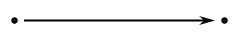
\includegraphics[width=0.8\linewidth]{figures/intro/scg/arcs/const/scg_const_perm_positive2.png}} & \parbox[|c]{2cm}{\centering\ni} & \parbox[|m]{2cm}{\centering\in} & \parbox[|c]{2cm}{\centering->} & \parbox[|m|]{2cm}{\centering<-} \\
	\hline
	
	\parbox[m|]{4.6cm}{\textit{\\ константная постоянная негативная sc-дуга принадлежности \\}} & \parbox[m|]{3.5cm}{\centering 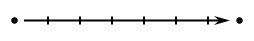
\includegraphics[width=0.8\linewidth]{figures/intro/scg/arcs/const/scg_const_perm_negative2.png}} & \parbox[m]{2cm}{\centering \not\ni} & \parbox[m|]{2cm}{\centering\notin} & \parbox[m|]{2cm}{\centering-|>} & \parbox[m]{2cm}{\centering<|-} \\
	\hline
	
	\parbox[m]{4.6cm}{\textit{\\ константная постоянная нечеткая sc-дуга принадлежности \\}} & \parbox[m]{3.5cm}{\centering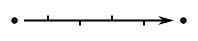
\includegraphics[width=0.8\linewidth]{figures/intro/scg/arcs/const/scg_const_perm_fuzzy2.png}} & \parbox[m]{2cm}{\centering / \ni} & \parbox[m]{2cm}{\centering \in /} & \parbox[m]{2cm}{\centering -/>} & \parbox[m]{2cm}{\centering </-} \\
	\hline
	
	\parbox[m]{4.6cm}{\textit{\\ константная временная позитивная sc-дуга принадлежности \\}} & \parbox[m]{3.5cm}{\centering 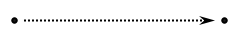
\includegraphics[width=0.8\linewidth]{figures/intro/scg/arcs/const/scg_const_temp_positive2.png}} & \parbox[m]{2cm}{\centering \sim \ni} & \parbox[m]{2cm}{\centering \in \sim} & \parbox[m]{2cm}{\centering \sim>} & \parbox[m]{2cm}{\centering <\sim} \\
	\hline
	
	\parbox[m]{4.6cm}{\textit{\\ константная временная негативная sc-дуга принадлежности \\}} & \parbox[m]{3.5cm}{\centering 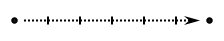
\includegraphics[width=0.8\linewidth]{figures/intro/scg/arcs/const/scg_const_temp_negative2.png}} & \parbox[m]{2cm}{\centering \sim \not\ni} & \parbox[m]{2cm}{\centering \notin \sim} & \parbox[m]{2cm}{\centering \sim|>} & \parbox[m]{2cm}{\centering <|\sim} \\
	\hline
	
	\parbox[m]{4.6cm}{\textit{\\ константная временная нечеткая sc-дуга принадлежности \\}} & \parbox[m]{3.5cm}{\centering 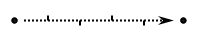
\includegraphics[width=0.8\linewidth]{figures/intro/scg/arcs/const/scg_const_temp_fuzzy2.png}} & \parbox[m]{2cm}{\centering \sim / \ni}  & \parbox[m]{2cm}{\centering \in/\sim} & \parbox[m]{2cm}{\centering \sim/>} & \parbox[m]{2cm}{\centering </\sim} \\
	\hline
	
	\parbox[m]{4.6cm}{\textit{\\ переменная постоянная позитивная sc-дуга принадлежности \\}} & \parbox[m]{3.5cm}{\centering 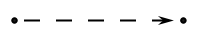
\includegraphics[width=0.8\linewidth]{figures/intro/scg/arcs/var/scg_var_perm_positive2.png}} & \parbox[m]{2cm}{\centering \textunderscore \ni} & \parbox[m]{2cm}{\centering \textunderscore \in} & \parbox[m]{2cm}{\centering \textunderscore->} & \parbox[m]{2cm}{\centering <-\textunderscore} \\
	\hline
	
	\parbox[m]{4.6cm}{\textit{\\ переменная постоянная негативная sc-дуга принадлежности \\}} & \parbox[m]{3.5cm}{\centering 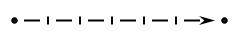
\includegraphics[width=0.8\linewidth]{figures/intro/scg/arcs/var/scg_var_perm_negative2.png}} & \parbox[m]{2cm}{\centering \textunderscore \not\ni} & \parbox[m]{2cm}{\centering \notin \textunderscore} & \parbox[m]{2cm}{\centering \textunderscore-|>} & \parbox[m]{2cm}{\centering <|-\textunderscore} \\
	\hline
	
	\parbox[m]{4.6cm}{\textit{\\ переменная постоянная нечеткая sc-дуга принадлежности \\}} & \parbox[m]{3.5cm}{\centering 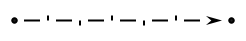
\includegraphics[width=0.8\linewidth]{figures/intro/scg/arcs/var/scg_var_perm_fuzzy2.png}} & \parbox[m]{2cm}{\centering \textunderscore /\ni} & \parbox[m]{2cm}{\centering \in/\textunderscore} & \parbox[m]{2cm}{\centering \textunderscore-/>} & \parbox[m]{2cm}{\centering </-\textunderscore} \\
	\hline
	
	\parbox[m]{4.6cm}{\textit{\\ переменная временная позитивная sc-дуга принадлежности \\}} & \parbox[m]{3.5cm}{\centering 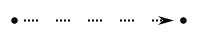
\includegraphics[width=0.8\linewidth]{figures/intro/scg/arcs/var/scg_var_temp_positive2.png}} & \parbox[m]{2cm}{\centering \textunderscore \sim \ni} & \parbox[m]{2cm}{\centering \in \sim \textunderscore} & \parbox[m]{2cm}{\centering \textunderscore \sim >} & \parbox[m]{2cm}{\centering < \sim \textunderscore} \\
	\hline
	
	\parbox[m]{4.6cm}{\textit{\\ переменная временная негативная sc-дуга принадлежности \\}} & \parbox[m]{3.5cm}{\centering 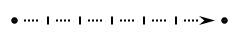
\includegraphics[width=0.8\linewidth]{figures/intro/scg/arcs/var/scg_var_temp_negative2.png}} & \parbox[m]{2cm}{\centering \textunderscore \sim \not$\ni$} & \parbox[c]{2cm}{\centering \notin \sim \textunderscore} & \parbox[m]{2cm}{\centering \textunderscore \sim |>} & \parbox[m]{2cm}{\centering <| \sim \textunderscore} \\
	\hline
	
	\parbox[m]{4.6cm}{\textit{\\переменная временная нечеткая sc-дуга принадлежности\\}} & \parbox[m]{3.5cm}{\centering 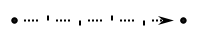
\includegraphics[width=0.8\linewidth]{figures/intro/scg/arcs/var/scg_var_temp_fuzzy2.png}} & \parbox[m]{2cm}{\centering \textunderscore \sim / \ni} & \parbox[m]{2cm}{\centering \in/\sim\textunderscore} & \parbox[m]{2cm}{\centering \textunderscore \sim />} & \parbox[m]{2cm}{\centering </\sim \textunderscore} \\
	\hline
	
	\parbox[m]{4.6cm}{\textit{\\метапеременная постоянная позитивная sc-дуга принадлежности\\}} & \parbox[m]{3.5cm}{\centering 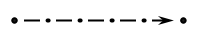
\includegraphics[width=0.8\linewidth]{figures/intro/scg/arcs/meta/scg_metavar_perm_positive2.png}} & \parbox[m]{2cm}{\centering\textunderscore \textunderscore\ni} & \parbox[m]{2cm}{\centering\in\textunderscore\textunderscore} & \parbox[m]{2cm}{\centering\textunderscore\textunderscore->} & \parbox[m]{2cm}{\centering <-\textunderscore\textunderscore} \\
	\hline
	
	\parbox[m]{4.6cm}{\textit{\\ метапеременная постоянная негативная sc-дуга принадлежности \\}} & \parbox[m]{3.5cm}{\centering 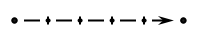
\includegraphics[width=0.8\linewidth]{figures/intro/scg/arcs/meta/scg_metavar_perm_negative2.png}} & \parbox[m]{2cm}{\centering \textunderscore\textunderscore \not\ni} & \parbox[m]{2cm}{\centering \notin\textunderscore\textunderscore} & \parbox[m]{2cm}{\centering \textunderscore\textunderscore-|>} & \parbox[m]{2cm}{\centering <|-\textunderscore\textunderscore} \\
	\hline
	
	\parbox[m]{4.6cm}{\textit{\\ метапеременная постоянная нечеткая sc-дуга принадлежности \\}} & \parbox[m]{3.5cm}{\centering 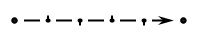
\includegraphics[width=0.8\linewidth]{figures/intro/scg/arcs/meta/scg_metavar_perm_fuzzy2.png}} & \parbox[m]{2cm}{\centering\textunderscore\textunderscore/\ni} & \parbox[m]{2cm}{\centering\in/\textunderscore\textunderscore} & \parbox[m]{2cm}{\centering\textunderscore\textunderscore-/>} & \parbox[m]{2cm}{\centering </-\textunderscore\textunderscore} \\
	\hline
	
	\parbox[m]{4.6cm}{\textit{\\ метапеременная временная позитивная sc-дуга принадлежности \\}} & \parbox[m]{3.5cm}{\centering 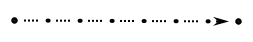
\includegraphics[width=0.8\linewidth]{figures/intro/scg/arcs/meta/scg_metavar_temp_positive2.png}} & \parbox[m]{2cm}{\centering\textunderscore\textunderscore\sim\ni} & \parbox[m]{2cm}{\centering\in\sim\textunderscore\textunderscore} & \parbox[m]{2cm}{\centering\textunderscore\textunderscore\sim>} & \parbox[m]{2cm}{\centering <\sim\textunderscore\textunderscore} \\
	\hline
	
	\parbox[m]{4.6cm}{\textit{\\ метапеременная временная негативная sc-дуга принадлежности \\}} & \parbox[m]{3.5cm}{\centering 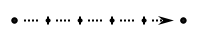
\includegraphics[width=0.8\linewidth]{figures/intro/scg/arcs/meta/scg_metavar_temp_negative2.png}} & \parbox[m]{2cm}{\centering \textunderscore\textunderscore\sim \not\ni} & \parbox[m]{2cm}{\centering\notin\sim\textunderscore\textunderscore} & \parbox[m]{2cm}{\centering\textunderscore\textunderscore\sim|>} & \parbox[m]{2cm}{\centering <|\sim\textunderscore\textunderscore} \\
	\hline
	
	\parbox[m]{4.6cm}{\textit{\\ метапеременная временная нечеткая sc-дуга принадлежности \\}} & \parbox[m]{3.5cm}{\centering 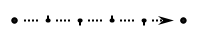
\includegraphics[width=0.8\linewidth]{figures/intro/scg/arcs/meta/scg_metavar_temp_fuzzy2.png}} & \parbox[m]{2cm}{\centering \textunderscore\textunderscore\sim/\ni} & \parbox[m]{2cm}{\centering\in/\sim\textunderscore\textunderscore} & \parbox[m]{2cm}{\centering\textunderscore\textunderscore\sim/>} & \parbox[m]{2cm}{\centering</\sim\textunderscore\textunderscore} \\
	\hline
\end{longtable}
}
%---------------------------------------------
\scnheader{Таблица. Алфавит sc.s-коннекторов, соответствующих sc.g-коннекторам, которые не являются sc.g-дугами принадлежности}
\scneqtable{
\begin{longtable}[l]{|m{6.2cm}|m{2.5cm}|m{2.5cm}|m{2.5cm}|m{2.5cm}|}
	\hline
	\multicolumn{1}{|c}{\parbox[c]{6.2cm}{Изображение \textit{\mbox{sc-коннектора}} в SCg}} &
	\multicolumn{2}{|c}{\parbox[c]{5cm}{Изображение \textit{\mbox{sc.s-коннектора}} в Расширенном алфавите}} &
	\multicolumn{2}{|c|}{\parbox[c]{5cm}{Изображение \textit{\mbox{sc.s-коннектора}} в Базовом алфавите}}
	\hline
	\endhead
	
	\parbox[|c]{6.2cm}{\\\centering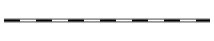
\includegraphics[width=0.8\linewidth]{figures/intro/scs/sc.s-connectors/noorient.png}\\} & \multicolumn{2}{c|}{ \parbox[c]{5cm}{\centering\leftrightarrow}} & \multicolumn{2}{c|}{ \parbox[c]{5cm}{\centering<>}} \\
	\hline
	
	\parbox[c]{6.2cm}{\\\centering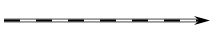
\includegraphics[width=0.8\linewidth]{figures/intro/scs/sc.s-connectors/orient.png} \\} &\parbox[c]{2.5cm}{\\\centering\rightarrow\\} & \parbox[c]{2.5cm}{\\\centering\leftarrow\\} & \parbox[c]{2.5cm}{\\\centering >>\\} & \parbox[c|]{2.5cm}{\\\centering <<\\} \\
	\hline
	
	\parbox[c]{6.2cm}{\\\centering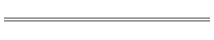
\includegraphics[width=0.8\linewidth]{figures/intro/scs/sc.s-connectors/constPermNoorien.png}\\} & \multicolumn{2}{c|}{\parbox[c]{5cm}{\centering\Leftrightarrow}} & \multicolumn{2}{c|}{\parbox[c]{5cm}{\centering<=>}} \\
	\hline
	
	\parbox[c]{6.2cm}{\\\centering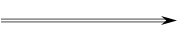
\includegraphics[width=0.8\linewidth]{figures/intro/scs/sc.s-connectors/constPermOrient.png}\\} & \parbox[c]{2.5cm}{\centering\Rightarrow} & \parbox[c]{2.5cm}{\centering\Leftarrow} & \parbox[c]{2.5cm}{\centering =>} & \parbox[c|]{2.5cm}{\centering <=} \\
	\hline
	
	\parbox[c]{6.2cm}{\\\centering
\includegraphics[width=0.8\linewidth]{figures/intro/scs/sc.s-connectors/constTempNoorien.png}\\} & \multicolumn{2}{c|}{\parbox[c]{5cm}{\centering\sim\Leftrightarrow}} & \multicolumn{2}{c|}{\parbox[c|]{5cm}{\centering\sim<=>}} \\
	\hline
	
	\parbox[c]{6.2cm}{\\\centering 
\includegraphics[width=0.8\linewidth]{figures/intro/scs/sc.s-connectors/constTempOrient.png}\\} & \parbox[c]{2.5cm}{\centering\sim\Rightarrow} & \parbox[c]{2.5cm}{\centering\Leftarrow\sim} & \parbox[c]{2.5cm}{\centering\sim=>} & \parbox[c|]{2.5cm}{\centering <=\sim} \\
	\hline
	
	\parbox[c]{6.2cm}{\\\centering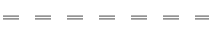
\includegraphics[width=0.8\linewidth]{figures/intro/scs/sc.s-connectors/varPermNoorien.png}\\} & \multicolumn{2}{c|}{\parbox[c]{5cm}{\centering\textunderscore\Leftrightarrow}} & \multicolumn{2}{c|}{\parbox[c|]{5cm}{\centering\textunderscore<=>}} \\
	\hline
	
	\parbox[c]{6.2cm}{\\\centering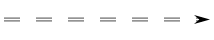
\includegraphics[width=0.8\linewidth]{figures/intro/scs/sc.s-connectors/varPermOrient.png}\\} & \parbox[c]{2.5cm}{\centering\textunderscore\Rightarrow} & \parbox[c]{2.5cm}{\centering\Leftarrow\textunderscore} & \parbox[c]{2.5cm}{\centering\textunderscore=>} & \parbox[c|]{2.5cm}{\centering <=\textunderscore} \\
	\hline
	
	\parbox[c]{6.2cm}{\\\centering
\includegraphics[width=0.8\linewidth]{figures/intro/scs/sc.s-connectors/varTempNoorien.png}\\} & \multicolumn{2}{c|}{\parbox[c]{5cm}{\centering\textunderscore\sim\Leftrightarrow}} & \multicolumn{2}{c|}{\parbox[c]{5cm}{\centering\textunderscore\sim<=>}} \\
	\hline
	
	\parbox[c]{6.2cm}{\\\centering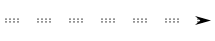
\includegraphics[width=0.8\linewidth]{figures/intro/scs/sc.s-connectors/varTempOrient.png}\\} & \parbox[c]{2.5cm}{\centering\textunderscore\sim\Rightarrow} & \parbox[c]{2.5cm}{\centering\Leftarrow\sim\textunderscore} & \parbox[c]{2.5cm}{\centering\textunderscore\sim=>} & \parbox[c|]{2.5cm}{\centering <=\sim\textunderscore} \\
	\hline
	
	\parbox[c]{6.2cm}{\\\centering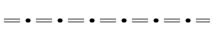
\includegraphics[width=0.8\linewidth]{figures/intro/scs/sc.s-connectors/metaPermNoorien.png}\\} & \multicolumn{2}{c|}{\parbox[c]{5cm}{\centering\textunderscore\textunderscore\Leftrightarrow}} & \multicolumn{2}{c|}{\parbox[c|]{5cm}{\centering\textunderscore\textunderscore<=>}} \\
	\hline
	
	\parbox[c]{6.2cm}{\\\centering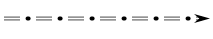
\includegraphics[width=0.8\linewidth]{figures/intro/scs/sc.s-connectors/metaPermOrient.png}\\} & \parbox[c]{2.5cm}{\centering\textunderscore\textunderscore\Rightarrow} & \parbox[c]{2.5cm}{\centering\Leftarrow\textunderscore\textunderscore} & \parbox[c]{2.5cm}{\centering\textunderscore\textunderscore=>} & \parbox[c|]{2.5cm}{\centering <=\textunderscore\textunderscore} \\
	\hline
	
	\parbox[c]{6.2cm}{\\\centering
\includegraphics[width=0.8\linewidth]{figures/intro/scs/sc.s-connectors/metaTempNoorien.png}\\} & \multicolumn{2}{c|}{\parbox[c]{5cm}{\centering\textunderscore\textunderscore\sim\Leftrightarrow}} & \multicolumn{2}{c|}{\parbox[c]{5cm}{\centering\textunderscore\textunderscore\sim<=>}} \\
	\hline
	
	\parbox[c]{6.2cm}{\\\centering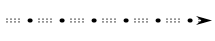
\includegraphics[width=0.8\linewidth]{figures/intro/scs/sc.s-connectors/metaTempOrient.png}\\} & \parbox[c]{2.5cm}{\centering\textunderscore\textunderscore\sim\Rightarrow} & \parbox[c]{2.5cm}{\centering\Leftarrow\sim\textunderscore\textunderscore} & \parbox[c]{2.5cm}{\centering\textunderscore\textunderscore\sim\Rightarrow} & \parbox[c|]{2.5cm}{\centering\Leftarrow\sim\textunderscore\textunderscore} \\
	\hline
	
	\parbox[c]{6.2cm}{\\\centering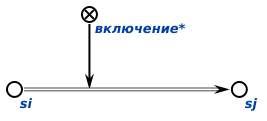
\includegraphics[width=0.8\linewidth]{figures/intro/scs/sc.s-connectors/examples/scs_transf_inclusion_const.png}\\} & \parbox[c]{2.5cm}{\centering\supseteq} & \parbox[c]{2.5cm}{\centering\subseteq} & \multicolumn{2}{c|}{\parbox[c]{5cm}{}} \\
	\hline
	
	\parbox[c]{6.2cm}{\\\centering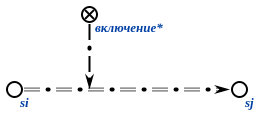
\includegraphics[width=0.8\linewidth]{figures/intro/scs/sc.s-connectors/examples/scs_transf_inclusion_meta.png}\\} & \parbox[c]{2.5cm}{\centering\textunderscore\supseteq} & \parbox[c]{2.5cm}{\centering\subseteq\textunderscore} & \multicolumn{2}{c|}{\parbox[c|]{5cm}{\centering}} \\
	\hline
	
	\parbox[c]{6.2cm}{\\\centering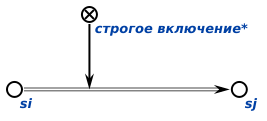
\includegraphics[width=0.8\linewidth]{figures/intro/scs/sc.s-connectors/examples/scs_transf_strict_inclusion_const.png}\\} & \parbox[c]{2.5cm}{\centering\supset} & \parbox[c]{2.5cm}{\centering\subset} & \multicolumn{2}{c|}{\parbox[c|]{5cm}{}} \\
	\hline
	
	\parbox[c]{6.2cm}{\\\centering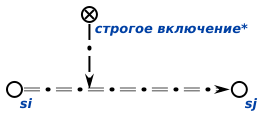
\includegraphics[width=0.8\linewidth]{figures/intro/scs/sc.s-connectors/examples/scs_transf_strict_inclusion_meta.png}\\} & \parbox[c]{2.5cm}{\centering\textunderscore\supset} & \parbox[c]{2.5cm}{\centering\subset\textunderscore} & \multicolumn{2}{c|}{\parbox[c|]{5cm}{}} \\
	\hline
	
	\parbox[c]{6.2cm}{\\\centering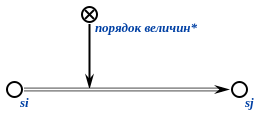
\includegraphics[width=0.8\linewidth]{figures/intro/scs/sc.s-connectors/examples/scs_transf_value_order_const.png}\\} & \parbox[c]{2.5cm}{\centering\geq} & \parbox[c]{2.5cm}{\centering\leq} & \multicolumn{2}{c|}{\parbox[c|]{5cm}{}} \\
	\hline
	
	\parbox[c]{6.2cm}{\\\centering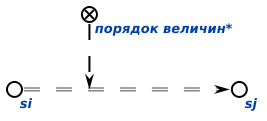
\includegraphics[width=0.8\linewidth]{figures/intro/scs/sc.s-connectors/examples/scs_transf_value_order_var.png}\\} & \parbox[c]{2.5cm}{\centering\textunderscore\geq} & \parbox[c]{2.5cm}{\centering\textunderscore\leq} & \multicolumn{2}{c|}{\parbox[c]{5cm}{}}  \\
	\hline
	
	\parbox[c]{6.2cm}{\\\centering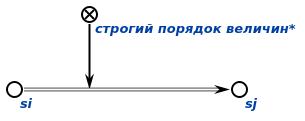
\includegraphics[width=0.8\linewidth]{figures/intro/scs/sc.s-connectors/examples/scs_transf_value_strict_order_const.png}\\} & \parbox[c]{2.5cm}{\centering >} & \parbox[c]{2.5cm}{\centering <} & \multicolumn{2}{c|}{\parbox[c]{5cm}{}} \\
	\hline
	
	\parbox[c]{6.2cm}{\\\centering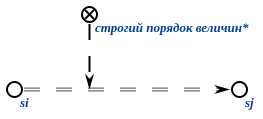
\includegraphics[width=0.8\linewidth]{figures/intro/scs/sc.s-connectors/examples/scs_transf_value_strict_order_var.png}\\} & \parbox[c]{2.5cm}{\centering\textunderscore>} & \parbox[c]{2.5cm}{\centering <\textunderscore} & \multicolumn{2}{c|}{\parbox[c]{5cm}{}} \\
	\hline
	
	\parbox[c]{6.2cm}{\\\centering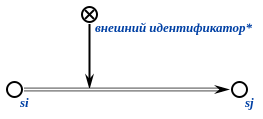
\includegraphics[width=0.8\linewidth]{figures/intro/scs/sc.s-connectors/examples/scs_transf_external_idtf_const.png}\\} & \multicolumn{2}{c|}{\parbox[c]{5cm}{\centering :=}} & \multicolumn{2}{c|}{\parbox[c]{5cm}{}} \\
	\hline
	
	\parbox[c]{6.2cm}{\\\centering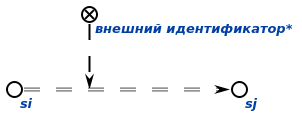
\includegraphics[width=0.8\linewidth]{figures/intro/scs/sc.s-connectors/examples/scs_transf_external_idtf_var.png}\\} & \multicolumn{2}{c|}{\parbox[c]{5cm}{\centering\textunderscore:=}} & \multicolumn{2}{c|}{\parbox[c]{5cm}{}} \\
	\hline
	
	\parbox[c]{6.2cm}{\\\centering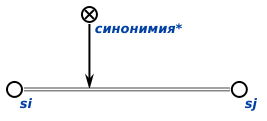
\includegraphics[width=0.8\linewidth]{figures/intro/scs/sc.s-connectors/examples/scs_transf_synonymy_const.png}\\} & \multicolumn{2}{c|}{\parbox[c]{5cm}{\centering =}} & \multicolumn{2}{c|}{\parbox[c]{5cm}{}} \\
	\hline
	
	\parbox[c]{6.2cm}{\\\centering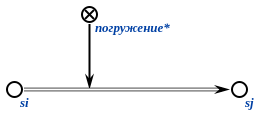
\includegraphics[width=0.8\linewidth]{figures/intro/scs/sc.s-connectors/examples/scs_transf_insertion_const.png}\\} & \parbox[c]{2.5cm}{\centering\supset=} & \parbox[c]{2.5cm}{\centering = \subset} &  \multicolumn{2}{c|}{\parbox[c]{5cm}{}}  \\
	\hline
\end{longtable}
}

\bigskip
\scnendstruct \scnendsegmentcomment{Описание sc.s-разделителей и sc.s-ограничителей}

\scnsegmentheader{Описание sc.s-предложений}
\scnstartsubstruct

\scnheader{sc.s-предложение}
\scnidtf{минимальный семантически целостный фрагмент sc.s-текста}
\scnidtf{минимальный sc.s-текст}
\scnsubset{sc.s-текст}
\scnsuperset{простое sc.s-предложение\\
    \scnaddlevel{1}
    \scnidtf{минимальное sc.s-предложение}
    \scnexplanation{\textit{sc.s-предложение}, (1) \uline{состоящее} или из двух \textit{sc-идентификаторов}, соединенных между собой \textit{\mbox{sc.s-коннектором}}, или из трех \textit{sc-идентификаторов}, разделенных \textit{sc.s-разделителями, изображающими связь инцидентности sc-элементов}, и (2) завершающееся \textit{двойной точкой с запятой}}
    \scnnote{Нетрудно заметить, что простые sc.s-предложения по сути аналогичны триплетам языка RDF (\mbox{RDF-триплетам}), за тем исключением, что \textit{простое sc.s-предложение} можно "развернуть"\ при помощи \textit{Операции конверсии sc.s-предложений*} не меняя при этом его смысл, а RDF-триплет нельзя. Это является одной из причин, по которой, в отличие от RDF-триплетов, в простых \mbox{sc.s-предложениях} \textit{\mbox{sc.s-коннекторы}} и \textit{\mbox{sc.s-разделители}, изображающие связь инцидентности \mbox{sc-элементов}} не могут быть опущены, поскольку они в том числе показывают направление изображаемой ими связи между sc-элементами.}
\scnrelfromlist{пример}{
    \scnfileitem{\textit{многоугольник} $\supset$ \textit{треугольник}}
    \scnaddlevel{1}
    \scnrelboth{семантическая эквивалентность}{\scnfilescg{figures/intro/scs/inclusion.png}}
    \scnaddlevel{-1};
    \scnfileitem{\textit{сторона*} $\ni$ (\textit{Четырехугк(ТчкА\char59ТчкВ\char59ТчкС\char59ТчкD)} $\Rightarrow$ \textit{Отр(ТчкВ\char59ТчкС)})\char59\char59}
    \scnaddlevel{1}
    \scnrelboth{семантическая эквивалентность}{\scnfilescg{figures/intro/scs/side.png}}
    \scnaddlevel{-1};
    \scnfileitem{\textit{Si} |- \textit{ai} >| \textit{ei}}
    \scnaddlevel{1}
    \scnrelboth{семантическая эквивалентность}{\scnfilescg{figures/intro/scs/inclusion_incident.png}}
    \scnaddlevel{-1}
    }
\scnaddlevel{-1}}
\scnnote{Признаком завершения любого \textit{sc.s-предложения}, т.е. последними его символами является \textit{двойная точка с запятой}, которую, следовательно, можно считать разделителем \textit{sc.s-предложений}.}
\scnrelfromlist{заданная операция}{Операция конверсии sc.s-предложения*\\
    \scnaddlevel{1}
    \scnsubset{синтаксическая трансформация*}
    \scnexplanation{Каждое \textit{sc.s-предложение} (в том числе, и \textit{простое sc.s-предложение}) можно преобразовать в семантически эквивалентное ему \textit{sc.s-предложение} путем конверсии ("разворота") цепочки компонентов \textit{sc.s-предложения}. Так, например, при конверсии ("развороте") простого \textit{\mbox{sc.s-предложения}} (1) первый его \textit{\mbox{sc-идентификатор}} (первый компонент этого \textit{\mbox{sc.s-предложения}}) становится третьим компонентом конвертированного\textit{ \mbox{sc.s-предложения}}, (2) второй его \textit{\mbox{sc-идентификатор}} (третий компонент исходного \textit{\mbox{sc.s-предложения}}) становится первым компонентом "конвертированного"\ \textit{\mbox{sc.s-предложения}} и (3) второй компонент исходного \textit{\mbox{sc.s-предложения}} (\textit{\mbox{sc.s-коннектор}} или \textit{\mbox{sc.s-разделитель}, изображающий связь инцидентности \mbox{sc-элементов}}, соединяющий указанные выше компоненты) остается вторым компонентом конвертированного \textit{\mbox{sc.s-предложения}}, но меняет направленность ("$\ni$"\ заменяется на "$\in$"\ и наоборот, "$\supset$"\ на "$\subset$"\ и наоборот, "$\Rightarrow$"\ на "$\Leftarrow$"\ и наоборот и т.д.)}
    \scnnote{Можно говорить не только о конверсии sc.s-предложения, но и о конверсии sc.s-коннектора, о конверсии sc.s-разделителя, изображающего связь инцидентности sc.s-элементов.}
    \scnrelfrom{sc.s-текст до трансформации}{\scnfilelong{\textit{треугольник $\ni$ Треуг(ТчкВ\char59ТчкС\char59ТчкD)}\char59\char59}}
    \scnrelfrom{sc.s-текст после трансформации}{\scnfilelong{\textit{Треуг(ТчкВ\char59ТчкС\char59ТчкD) $\in$ треугольник}\char59\char59}}
	\scnaddlevel{1}
    \scnrelboth{семантическая эквивалентность}{\scnfilescg{figures/intro/scs/conversion.png}}
    \scnaddlevel{-2}
;Операция присоединения sc.s-предложения*\\
    \scnaddlevel{1}
    \scnsubset{синтаксическая трансформация*}
    \scnidtf{Операция соединения двух sc.s-предложений при совпадении последнего компонента первого предложения с первым компонентом второго*}
    \scnexplanation{В результате выполнения данной операции:
    \begin{scnitemize}
        \item первый компонент второго sc.s-предложения удаляется\char59
        \item оставшаяся часть второго предложения окружается sc.s-ограничителем присоединенных предложений ("(*"\ и "*)"). Разделитель sc.s-предложений (";;") также попадает внутрь указанного ограничителя\char59
        \item полученная конструкция помещается между последним компонентом первого предложения и разделителем sc.s-предложений, которым заканчивалось первое предложение\char59
        \item второе предложение, таким образом, становится присоединенным sc.s-предложением.
    \end{scnitemize}
    Аналогичным образом к любому присоединенному sc.s-предложению могут "пристыковываться"\ другие присоединенные sc.s-предложения, в общем случае уровень такой вложенности не ограничен.
    }
    \scnaddlevel{-1}
;Операция слияния sc.s-предложений*\\
    \scnaddlevel{1}
    \scnsubset{синтаксическая трансформация*}
    \scnidtf{Операция присоединения простого sc.s-предложения к sc.s-предложению, у которого последний sc.s-коннектор совпадает с sc.s-коннектором простого sc.s-предложения, а предшествующий указанному sc.s-коннектору sc-идентификатор совпадает с первым sc-идентификатором простого sc.s-предложения*}
    \scnexplanation{В результате выполнения этой операции совпадающие sc-идентификаторы и sc.s-коннекторы соединяемых sc.s-предложений "склеиваются"\ , а последние sc-иден\-ти\-фи\-ка\-то\-ры соединяемых \textit{sc.s-предложений} становятся последними компонентами объединенного \textit{sc.s-предложения},
    разделенными \textit{точкой с запятой}. Аналогичным образом можно присоединять сколько угодно простых \textit{sc.s-предложений}.}
    \scnaddlevel{-1}
;Операция разложения sc.s-предложений на простые sc.s-предложения*\\
    \scnaddlevel{1}
    \scnsubset{синтаксическая трансформация*}
    \scnexplanation{Каждое \textit{sc.s-предложение} можно разложить на множество \textit{простых sc.s-предложений}, т.е. представить в виде последовательности \textit{простых sc.s-предложений}.}
    \scnaddlevel{-1}
;Операция разложения sc.s-предложений на простые sc.s-предложения с sc.s-разделителем, изображающим связь инцидентности sc-элементов*\\
    \scnaddlevel{1}
    \scnsubset{синтаксическая трансформация*}
    \scnexplanation{Каждое \textit{sc.s-предложение} (в том числе и \textit{простое sc.s-предложение} с \textit{sc.s-коннектором}) можно представить в виде семантически эквивалентной последовательности \textit{простых \mbox{sc.s-предложений}} с \textit{sc.s-разделителем, изображающим связь инцидентности \mbox{sc-элементов}}.}
    \scnnote{Данная операция осуществляет \uline{однозначное} (!) формирование множества \textit{простых \mbox{sc.s-предложений}} указанного вида.}
    \scnaddlevel{-1}
    }

\newpage
\scnheader{sc.s-предложение}
\scnnote{Операции, заданные на множестве \textit{sc.s-предложений} можно разделить на три группы:
    \begin{scnitemize}
        \item группа операций конверсии \textit{sc.s-предложений}, состоящая из одной операции;
        \item группа операций соединения \textit{sc.s-предложений};
        \item группа операций декомпозиции \textit{sc.s-предложений} и, в частности, операций разложения \textit{sc.s-предложений}.
    \end{scnitemize}
Очевидно, что операции соединения \textit{sc.s-предложений} и операции декомпозиции \textit{sc.s-предложений} являются обратными друг другу операциями.}
\scnaddlevel{-1}

\scnheader{Описание примеров выполнения операций, заданных на множестве sc.s-предложений}
\scnstartsubstruct

\bigskip

\scnfilelong{\textit{треугольник $\ni$ Треугк(ТчкВ\char59ТчкС\char59ТчкD)}\char59\char59}
\scnrelfrom{Операция конверсии sc.s-предложения}{\scnfilelong{\textit{Треугк(ТчкВ\char59ТчкС\char59ТчкD) $\in$ треугольник}\char59\char59}}
\scnaddlevel{1}
\scnrelboth{семантическая эквивалентность}{\scnfilescg{figures/intro/scs/conversion.png}}
\scnaddlevel{-1}

\bigskip\bigskip

{\scnfilelong{\textit{треугольник $\ni$ Треугк(ТчкВ\char59ТчкС\char59ТчкD)\char59\char59
\newline
Треугк(ТчкВ\char59ТчкС\char59ТчкD) $\Rightarrow$ сторона*:включение*: Отр(ТчкВ\char59ТчкC)\char59\char59}}}
\scnrelfrom{Операция присоединения sc.s-предложения}{\scnfilelong{\textit{треугольник $\ni$ Треугк(ТчкВ\char59ТчкС\char59ТчкD) (* $\Rightarrow$ сторона*:включение*:Отр(ТчкВ\char59ТчкС)\char59\char59*) }\char59\char59}}
\scnaddlevel{1}
\scnrelboth{семантическая эквивалентность}{\scnfilescg{figures/intro/scs/joining_sentences.png}}
\scnaddlevel{-1}

\bigskip\bigskip

\scnfilelong{\textit{сторона* $\ni$ (Треугк(ТчкВ\char59Тчк С\char59ТчкD) $\Rightarrow$ Отр(ТчкВ\char59ТчкС))\char59\char59
\newline
сторона* $\ni$ (Треугк(ТчкВ\char59Тчк С\char59ТчкD) $\Rightarrow$ Отр(ТчкC\char59ТчкD))\char59\char59}}
\scnrelfrom{Операция слияния sc.s-предложений}{\scnfilelong{\textit{сторона* $\ni$ ((Треугк(ТчкВ\char59ТчкС\char59ТчкD) $\Rightarrow$ Отр(ТчкВ\char59ТчкС))\char59(Треуг(ТчкВ\char59ТчкС\char59ТчкD) $\Rightarrow$ Отр(ТчкC\char59ТчкD)))\char59\char59}}}
\scnaddlevel{1}
\scnrelfrom{синтаксическая трансформация}{\scnfilelong{\textit{Треугк(ТчкВ\char59ТчкС\char59ТчкD)}$\Rightarrow$\textit{сторона*}: \textit{Отр(ТчкВ\char59ТчкС)}\char59\textit{Отр(ТчкС\char59ТчкD)}\char59\char59}}
\scnrelboth{семантическая эквивалентность}{\scnfilescg{figures/intro/scs/joining_sentence.png}}
\scnaddlevel{-1}

\bigskip\bigskip

\newpage
{\scnfilelong{\textit{Треугк(ТчкВ\char59ТчкС\char59ТчкD) $\Rightarrow$ сторона*:включение*:Отр(ТчкВ\char59ТчкС)\char59\char59}}}
\scnrelfrom{Операция разложения sc.s-предложений на простые sc.s-предложения}{\scnfilelong{\textit{сторона* $\ni$ (Треугк(ТчкВ\char59ТчкС\char59ТчкD) $\Rightarrow$ Отр(ТчкВ\char59ТчкС))\char59\char59
\newline включение* $\ni$ (Треугк(ТчкВ\char59ТчкС\char59ТчкD) $\Rightarrow$ Отр(ТчкВ\char59ТчкС))\char59\char59}}}
\scnaddlevel{1}
\scnrelboth{семантическая эквивалентность}{\scnfilescg{figures/intro/scs/dividing_sentences.png}}
\scnaddlevel{-1}

\bigskip\bigskip

{\scnfilelong{\textit{треугольник $\ni$ Треугк(ТчкВ\char59ТчкC\char59ТчкD)}}}
\scnrelfrom{Операция разложения sc.s-предложений на простые sc.s-предложения с sc.s-разделителем, изображающим связь инцидентности sc-элементов}{\scnfilelong{\textit{треугольник |- ai >| Треугк(ТчкВ\char59ТчкС\char59ТчкD)\char59\char59
\newline
константный постоянный sc-узел, обозначающий класс $\ni$ треугольник\char59\char59
\newline
константная постоянная позитивная sc-дуга принадлежности $\ni$ ai\char59\char59
\newline
константный постоянный sc-узел общего вида $\ni$ Треугк(ТчкВ\char59ТчкC\char59ТчкD)\char59\char59}}}
\scnaddlevel{1}
\scnrelboth{семантическая эквивалентность}{\scnfilescg{figures/intro/scs/dividing_sentences_incident.png}}
\scnaddlevel{-1}

\scnendstruct

\scnheader{присоединенное sc.s-предложение}
\scnidtf{встроенное sc.s-предложение}
\scnexplanation{Присоединенные sc.s-предложения используются для того, чтобы продолжить спецификацию какого-либо sc-элемента, sc-идентификатор которого является последним компонентом в рамках какого-либо sc.s-предложения, не начиная при этом нового sc.s-предложения и, таким образом, не дублируя указанный \mbox{sc-идентификатор}. Внутрь присоединенных sc.s-предложений также могут встраиваться другие присоединенные sc.s-предложения, в общем случае уровень вложенности таких предложений не ограничен. Таким образом присоединенные sc.s-предложения описывают "ветвление"\ sc.s-предложений, при этом точками такого "ветвления"\ выступают sc-идентификаторы, входящие в состав этих sc.s-предложений.

Благодаря введению присоединенных sc.s-предложений появляется возможность любой sc-текст изобразить в виде одного sc.s-предложения, содержащего необходимое количество присоединенных sc.s-предложений. Таким образом, SCs-код по выразительной мощности становится эквивалентным SCn-коду.}

\scnheader{sc.s-предложение}
\scntext{денотационная семантика}{С семантической точки зрения \textit{sc.s-предложение} представляет собой описание некоторого \uline{маршрута} в соответствующем sc-тексте, который является графовой структурой специального вида и структура которого описывается (изображается) с помощью \textit{sc.s-предложений}. Указанный маршрут "проводится"\ по sc-коннекторам и по связям инцидентности sc-элементов, если маршрут проходит через инцидентные sc-коннекторы. В описании указанного маршрута могут дополнительно указываться множества (чаще всего отношения), которым принадлежат sc-коннекторы, входящие в описываемый маршрут. Кроме того, указанный маршрут в начале и/или в конце может иметь разветвления, когда какой-либо sc-элемент \uline{одинаково} инцидентен нескольким \uline{однотипным} sc-коннекторам, соединяющим указанный sc-элемент с некоторыми другими sc-элементами.

Таким образом каждое указанное разветвление состоит из неограниченного числа ветвей, каждая из которых состоит из одного sc-коннектора и одного связываемого им sc-элемента.}

\scnheader{компонент sc.s-предложения*}
\scnexplanation{Каждое \textit{sc.s-предложение} представляет собой последовательность (1) \textit{sc-идентификаторов}, \mbox{(2) \textit{sc.s-коннекторов}} или \textit{sc.s-разделителей}, изображающих связь инцидентности \textit{sc-элементов}, (3) \textit{точек с запятыми}, (4) \textit{ограничителей присоединенных sc.s-предложений}, завершаемая \textit{двойной точкой с запятой}. При этом непосредственно соседствовать друг с другом не могут ни \textit{\mbox{sc-идентификаторы}}, ни \textit{\mbox{sc.s-коннекторы}}, ни, очевидно, \textit{точки с запятыми} и \textit{ограничители присоединенных sc.s-предложений}.\\
Между \textit{sc-идентификаторами} в рамках \textit{sc.s-предложения} может находиться либо \textit{точка с запятой}, либо \textit{sc.s-коннектор}, либо \textit{sc.s-разделитель}, изображающий связь инцидентности \textit{sc-элементов}. Слева и справа от \textit{sc.s-коннектора} и от \textit{sc.s-разделителя}, изображающего связь инцидентности \textit{sc-элементов}, должны находиться \textit{sc-идентификаторы}.

Указанные \textit{sc-идентификаторы}, \textit{sc.s-коннекторы} и \textit{sc.s-разделители}, изображающие связь инцидентности \textit{sc-элементов}, считаются компонентами соответствующего \textit{sc.s-предложения}. Понятие "быть компонентом sc.s-предложения"\ является относительным понятием (отношением), т.к. в состав некоторых компонентов \textit{sc.s-предложения} (в состав \textit{sc-идентификаторов}, являющихся \textit{sc.s-выражениями}, ограничиваемыми фигурными или квадратными скобками) могут входить других \textit{sc.s-предложения}, состоящие из своих компонентов.}
\scnrelfrom{первый домен}{sc.s-предложение}
\scnrelfrom{второй домен}{{\normalfont (} sc-идентификатор $\cup$ sc.s-разделитель $\cup$ sc.s-ограничитель {\normalfont )}}

\scnheader{sc.s-модификатор*}
\scnsubset{компонент sc.s-предложения*}
\scnexplanation{Это дополнительный вид компонентов \textit{sc.s-предложений}. Каждый \textit{sc.s-модификатор}, являющийся компонентом некоторого \textit{sc.s-предложения}, представляет собой \textit{sc-идентификатор}, обозначающий множество (чаще всего, отношение), которому принадлежит sc-коннектор, изображенный \textit{sc.s-коннектором}, который предшествует указанному \textit{sc-идентификатору}. Признаком \textit{sc.s-модификатора} является \textit{двоеточие} (или \textit{двойное двоеточие}), которое ставится после \textit{sc.s-модификатора} и отделяет его либо от следующего за ним другого \textit{sc.s-модификатора} для этого же \textit{sc.s-коннектора}, либо от следующего за ним \textit{sc-идентификатора}, соответствующего sc-элементу, который инцидентен sc-коннектору, изображенному \textit{sc.s-коннектором}, находящимся левее рассматриваемого \textit{sc-идентификатора} после одного или нескольких \textit{sc.s-модификаторов}. Обычное ("одинарное") \textit{двоеточие} обозначает, что sc-элемент, изображенный соответствующим \mbox{sc.s-модификатором}, связан с sc-коннектором, изображенным левее этого \mbox{sc.s-модификатора}, \textit{базовой \mbox{sc-дугой}} (\textit{константной постоянной позитивной \mbox{sc-дугой} принадлежности}), \textit{двойное двоеточие} обозначает, что указанные элементы связаны \textit{переменной постоянной позитивной \mbox{sc-дугой} принадлежности}.}
\scnrelfromlist{пример}{
    \scnfileitem{\textit{Четырехугк(ТчкА;ТчкВ;ТчкС;ТчкD)} $\Rightarrow$ \textit{сторона*} : \textit{включение*} : \textit{Отр(ТчкВ;ТчкС)};; }\\
    \scnaddlevel{1}
    \scnrelboth{семантическая эквивалентность}{\scnfilescg{figures/intro/scs/modifier.png}}
    \scnaddlevel{-1}
    \newpage;
    \scnfileitem{\textit{Треугк(ТчкА;ТчкВ;ТчкС)} $\_\Rightarrow$ \textit{сторона*} :: \textit{\_s};; }\\
    \scnaddlevel{1}
    \scnrelboth{семантическая эквивалентность}{\scnfilescg{figures/intro/scs/modifier_var.png}}
    \scnaddlevel{-1}
    }

\scnheader{sc.s-текст}
\scnidtf{конкатенация \textit{sc.s-предложений}}
\scnidtf{последовательность \textit{sc.s-предложений}, разделяемых \textit{двойными точками с запятой}}
\scnsuperset{максимальный исходный sc.s-текст}
    \scnaddlevel{1}
    \scnidtf{конкатенция \textit{sc.s-предложений}, слева и справа от которой отсутствуют какие-либо символы SCs-кода}
    \scnaddlevel{-1}
\scnsuperset{максимальный sc.s-текст, включенный в структуру}
    \scnaddlevel{1}
    \scnidtf{конкатенция всех \textit{sc.s-предложений}, входящих в состав \textit{sc.s-выражения структуры}}
    \scnsuperset{sc.s-текст, включенный в структуру}
        \scnaddlevel{1}
        \scnidtf{часть цепочки \textit{sc.s-предложений}, входящих в состав максимального sc.s-текста, включенного в структуру}
        \scnsuperset{sc.s-предложение, включенное в структуру}
    \scnaddlevel{-2}
\scnnote{\textit{sc.s-предложение} является минимальным sc.s-текстом.}
\scntext{свойство}{Смысл sc.s-текста (а также \textit{sc.s-текста, включенного в структуру} не зависит от порядка \textit{\mbox{sc.s-предложений}} в этих sc-текстах. Т.е. перестановка \textit{\mbox{sc.s-предложений}} в рамках таких \mbox{sc.s-текстов} смысла этих \mbox{sc.s-текстов} не меняет (т.е. приводит к семантически эквивалентным \mbox{sc.s-текстам}), но сильно влияет на трудоемкость человеческого восприятия (на "читабельность") этих текстов.}
\scnrelfrom{пример}{\scnfilelong{
		\textit{материальный объект} $\ni$ \textit{Земля} (* => \textit{вращаться вокруг}*: \textit{спутник}*: \textit{Луна};;*);;\\
		\textit{материальный объект} $\ni$ \textit{Луна}(* => \textit{основной идентификатор}*: [Moon] (* <- \textit{Английский язык};; *); [Луна] (* <- \textit{Русский язык};; *);; *);;\\
		\textit{материальный объект} $\ni$ \textit{Солнце} (* => \textit{вращаться вокруг}*: \textit{Земля}; \textit{Марс};; *);;\\
		\textit{материальный объект} $\ni$ \textit{Марс};;}
}    
\scnaddlevel{1}
\scnrelfrom{семантическая эквивалентность}{ \scnfilescg{figures/intro/scs/scs_text_example.png}}
\scnaddlevel{-1}
    
\bigskip
\scnendstruct \scnendsegmentcomment{Завершили Описание sc.s-предложений}

\scnsegmentheader{Описание Ядра SCs-кода и различных направлений его расширения}
\scnstartsubstruct

\scnheader{Ядро SCs-кода}
\scnidtf{Подъязык SCs-кода, который использует минимальный набор синтаксических средств, но при этом имеет семантическую мощность, эквивалентную мощности SCs-кода в целом}
\scntext{принципы, лежащие в основе}{В Ядре SCs-кода:
\begin{scnitemize}
    \item используются только \textit{простые sc-идентификаторы}, в том числе \textit{sc-идентификаторы внешних файлов ostis-систем} (sc-выражения не используются);
    \item используются только \textit{sc.s-разделители, изображающие связь инцидентности sc-элементов}, а также sc.s-коннектор, изображающий константную  постоянную позитивную пару принадлежности ("$\in$" и "$\ni$" в Расширенном алфавите и "{}->{}"\ и "{}<-{}"\ в Базовом алфавите). Другие \textit{sc.s-коннекторы} не используются;
    \item не используются \textit{sc.s-модификаторы} и, соответственно, двоеточия, являющиеся признаком завершения \textit{sc.s-модификаторов};
    \item используются только \textit{простые sc.s-предложения}, которые, как следует из вышеуказанных свойств Ядра SCs-кода, либо состоят из двух \textit{простых sc-идентификаторов}, соединяемых sc.s-коннектором, изображающим константную  постоянную позитивную пару принадлежности, либо трех \textit{простых sc-идентификаторов}, разделенных \textit{sc.s-разделителями, изображающими связь инцидентности sc-элементов}.
\end{scnitemize}

Из перечисленных свойств Ядра SCs-кода следует, что для представления (изображения) любого \mbox{sc-текста} средствами Ядра SCs-кода необходимо для \uline{всех} (!) sc-элементов этого \mbox{sc-текста} (кроме константных постоянных позитивных пар принадлежности) построить соответствующие им простые \textit{sc-идентификаторы}, т.е. необходимо проименовать все указанные sc-элементы. В свою очередь, тип каждого используемого \mbox{sc-элемента} (кроме константных постоянных позитивных пар принадлежности) задается явно путем указания принадлежности этих элементов соответствующим классам sc-элементов, в том числе классам, входящим в Ядро SC-кода.

Как видно из приведенного описания, Ядро SCs-кода соответствует Ядру SCg-кода, за исключением того, что в Ядре SCg-кода нет необходимости именовать все изображаемые sc-элементы, а также в Ядре SCg-кода присутствуют графические изображения для sc-элементов, принадлежащих соответствующим классам Ядра SC-кода и эту принадлежность нет необходимости указывать явно.
}
\scnnote{Очевидно, что широко практически применять Ядро SCs-кода для записи больших фрагментов баз знаний неудобно и неэффективно. Тем не менее, с практической точки зрения Ядро SCs-кода может использоваться, например, для обмена информацией со сторонними средствами представления графовых конструкций, рассчитанными на представление информации в виде триплетов (например, RDF-хранилищ).
Для обеспечения возможности более широкого практического использования необходимы синтаксические расширения Ядра SCs-кода в целях:
\begin{scnitemize}
    \item минимизации числа идентифицируемых (именуемых) sc-элементов путем использования \textit{sc-выражений} и ликвидации необходимости идентифицировать (именовать) \uline{все} (!) sc-элементы;
    \item сокращения текста путем минимизации числа повторений одного и того же \textit{sc-идентификатора} путем соединения \textit{sc.s-предложений};
    \item повышение уровня наглядности, "читабельности"\ sc.s-текстов.
\end{scnitemize}}
\scnhaselementrole{пример}{\scnfilelong{\textit{треугольник |- ai >| Треугк(ТчкВ\char59ТчкС\char59ТчкD)\char59\char59
\newline
Треугк(ТчкВ\char59ТчкС\char59ТчкD) |- bi >| Отр(ТчкВ\char59ТчкС)\char59\char59
\newline
сторона* |- сi >| bi\char59\char59
\newline
константный постоянный sc-узел, обозначающий класс $\ni$ треугольник\char59\char59
\newline
константный постоянный sc-узел, обозначающий отношение $\ni$ сторона*\char59\char59
\newline
константная постоянная позитивная sc-дуга принадлежности $\ni$ ai\char59\char59
\newline
константная постоянная sc-дуга $\ni$ bi\char59\char59
\newline
константная постоянная позитивная sc-дуга принадлежности $\ni$ ci\char59\char59
\newline
константный постоянный sc-узел общего вида $\ni$ Отр(ТчкВ\char59ТчкС)\char59\char59
\newline
константный постоянный sc-узел общего вида $\ni$ Треугк(ТчкВ\char59ТчкC\char59ТчкD)\char59\char59}}}
\scnaddlevel{1}
\bigskip
\scnrelboth{семантическая эквивалентность}{\scnfilescg{figures/intro/scs/kernel_incident.png}}
\scnaddlevel{-1}

\scnheader{Первое направление расширения Ядра SCs-кода}
\scnidtf{Первое направление расширения Ядра SCs-кода \uline{и всех иных его расширений}}
\scntext{принципы}{По сравнению с \textit{Ядром SCs-кода} в \textit{Первом направлении расширения Ядра SCs-кода} вместо \textit{sc-идентификато|-ров}, являющихся идентификаторами (именами), которые взаимно однозначно соответствуют синонимичным им (представляемым ими) sc-коннекторам, вводятся \textit{sc.s-коннекторы}, каждый из которых соответствует не одному конкретному sc-коннектору, а некоторому классу однотипных sc-коннекторов. Очевидно, что это ликвидирует необходимость \uline{каждому} sc-коннектору приписывать уникальный \textit{sc-идентификатор}. Кроме того, \textit{Алфавит sc.s-коннекторов} включает в себя элементы этого Алфавита (классы \uline{синтаксически} эквивалентных \textit{sc.s-коннекторов}), которые соответствуют \uline{всем} (!) элементам Алфавита sc-коннекторов, но при этом дополнительно включают в себя и другие элементы Алфавита \textit{sc.s-коннекторов}, которые соответствуют часто используемым \uline{семантически} явно выделяемым классам sc-коннекторов. К таким дополнительно вводимым классам \textit{sc.s-коннекторов} относятся \textit{константные sc.s-коннекторы} включения множеств ("$\supset$"\ или "$\subset$"), \textit{переменные sc.s-коннекторы} включения множеств ("$\_\supset$"\ или "$\subset\_$"), \textit{sc.s-коннектор} синонимии ("$=$"), \textit{sc.s-коннектор} погружения ("$=\subset$"\ или "$\supset=$") и др.

Заметим, что указанное расширение Алфавита \textit{sc.s-коннекторов} аналогично расширенному Алфавиту \textit{sc.g-коннекторов} в SCg-коде и ликвидирует необходимость (как и в SCs-коде) явно специфицировать (средствами SCs-кода) синтаксически выделяемые классы \textit{sc.s-коннекторов}.}

\scnheader{Второе направление расширения Ядра SCs-кода}
\scntext{принципы}{Во Втором направлении расширения Ядра SCs-кода вводятся модификаторы \textit{sc.s-коннекторов} (\textit{\mbox{sc.s-модификаторы}}), которые позволяют достаточно компактно дополнительно специфицировать \mbox{sc-коннекторы}, изображаемые (представляемые) соответствующими \textit{sc.s-коннекторами}. Речь идет о такой часто востребованной форме спецификации sc-коннекторов, как указание множества (возможно, нескольких множеств), которому принадлежит специфицируемый  sc-коннектор (чаще всего, таким множеством является \textit{бинарное отношение} (в частности, \textit{ролевое отношение}) или \textit{квазибинарное отношение}).}

\scnheader{sc.s-модификатор*}
\scniselement{отношение}
    \scnaddlevel{1}
    \scnidtf{относительное понятие}
    \scnaddlevel{-1}
\scnidtf{модификатор sc.s-коннектора*}
\scnexplanation{\textit{sc-идентификатор}, который (1) находится либо между \textit{sc.s-коннектором} и \textit{двоеточием}, либо между \textit{двоеточиями} и (2) обозначает множество (чаще всего, отношение), которому принадлежит sc-коннектор, изображаемый ближайшим предшествующим \textit{sc.s-коннектором}. Два подряд идущих двоеточия ("::") обозначают, что указанное множество связано с указанным sc-коннектором \textit{\uline{переменной} позитивной постоянной sc-дугой принадлежности}.

Очевидно, что, если не использовать \textit{sc.s-модификаторы}, указанного вида спецификация sc-коннекторов средствами SCs-кода будет выглядеть значительно более громоздкой.}

\scnheader{Третье направление расширения Ядра SCs-кода}
\scntext{принципы}{В \textit{Третьем направлении расширения Ядра SCs-кода} осуществляется переход от использования только \textit{простых sc-идентификаторов} к использованию как \textit{простых sc-идентификаторов}, так и \textit{sc-выражений}, а также к использованию \textit{sc.s-представлений некоторых неидентифицируемых sc-узлов}. Это существенно сокращает число придумываемых \textit{простых sc-идентификаторов}, т.к. каждое \textit{sc-выражение} в конечном счете — это комбинация \textit{простых sc-идентификаторов}, построенная по правилам, которые достаточно легко семантически интерпретируются. Если проводить аналогию с SCg-кодом, то очевидно, что \textit{\mbox{sc-выражение}}, ограничиваемое фигурными скобками, есть не что иное, как информационная конструкция, ограничиваемая \textit{sc.g-контуром}, а \textit{sc-выражение}, ограничиваемое квадратными скобками есть не что иное, как информационная конструкция, ограничиваемая \textit{sc.g-рамкой}. Отличие здесь заключается в том, что круглыми и квадратными скобками можно ограничивать только линейные информационные конструкции (цепочки символов).}

\scnheader{sc.s-представление неидентифицируемого sc-узла}
\scnidtf{изображение (представление) неидентифицируемого (неименуемого) sc-узла в sc.s-тексте}
\scnidtf{sc.s-обозначение неименуемой сущности, не являющейся парой, обозначаемой sc-коннектором}
\scnidtf{sc.s-представление sc-узла, не являющееся sc-идентификатором (именем этого sc-узла)}
\scnreltoset{разбиение}{sc.s-обозначение неименуемой структуры\\
    \scnaddlevel{1}
    \scnidtf{конкатенация левой фигурной скобки и правой фигурной скобки}
    \scnaddlevel{-1}
;sc.s-обозначение неименуемой неориентированной связки\\
    \scnaddlevel{1}
    \scnidtf{конкатенация левой фигурной скобки, дефиса и правой фигурной скобки}
    \scnaddlevel{-1}
;sc.s-обозначение неименуемого кортежа\\
    \scnaddlevel{1}
    \scnidtf{конкатенация левой угловой скобки, дефиса и правой угловой скобки}
    \scnaddlevel{-1}
;sc.s-обозначение неименуемого файла-экземпляра\\
    \scnaddlevel{1}
    \scnidtf{конкатенация левой квадратной скобки и правой квадратной скобки}
    \scnaddlevel{-1}
;sc.s-обозначение неименуемого файла-класса\\
    \scnaddlevel{1}
    \scnidtf{конкатенация восклицательного знака, левой квадратной скобки и правой квадратной скобки}
    \scnaddlevel{-1}
;sc.s-обозначение неименуемой терминальной сущности\\
    \scnaddlevel{1}
    \scnidtf{конкатенация левой круглой скобки, буквы "о"\ и правой круглой скобки}
    \scnaddlevel{-1}}
\scntext{примечание}{Если одно и то же обозначение неименуемой сущности встречается в \uline{разных} \textit{sc.s-предложениях}, то считается, что это обозначения \uline{разных} сущностей, т.е. изображения \uline{разных} sc-узлов.}

\scnheader{Четвертое направление расширения Ядра SCs-кода}
\scntext{принципы}{В \textit{Четвертом направлении расширения Ядра SCs-кода} осуществляется переход от использования только \textit{простых sc.s-предложений} к использованию также \textit{sc.s-предложений}, построенных с помощью \textit{\mbox{Операции} присоединения sc.s-предложения*}. В результате этого, благодаря "склеиванию"\ одинаковых \textit{\mbox{sc-идентификаторов}}, а также "склеиванию"\ синтаксически эквивалентных \textit{\mbox{sc.s-коннекторов}} с одинаковыми \textit{\mbox{sc.s-модификаторами}} (несмотря на то, что эти "склеиваемые"\ \textit{sc.s-коннекторы} соответствуют \uline{разным} \mbox{sc-коннекторам}), существенно сокращается число копий используемых \textit{\mbox{sc-идентификаторов}} и \textit{\mbox{sc.s-коннекторов}} с их \textit{\mbox{sc.s-модификаторами}}.}

\newpage
\scnheader{Пятое направление расширения Ядра SCs-кода}
\scntext{принципы}{В \textit{Пятом направлении расширения Ядра SCs-кода} разрешается использование \textit{присоединенных \mbox{sc.s-предложений}}. В результате этого \textit{sc.s-тексты} становятся более компактными и удобными для восприятия за счет снижения числа дублируемых \textit{sc-идентификаторов} и более широких возможностей их структуризации.}

\scnheader{следует отличать*}
\scnhaselementset{sc.s-представление неидентифицируемого sc-узла;sc.s-коннектор\\
    \scnaddlevel{1}
    \scnidtf{sc.s-представление неидентифицируемого sc-коннектора}
    \scnaddlevel{-1}}\bigskip
\scnhaselementset{sc-коннектор;sc.s-коннектор}\bigskip
\scnhaselementset{sc.s-коннектор;sc.s-модификатор*\\
    \scnaddlevel{1}
    \scnidtf{модификатор sc.s-коннектора*}
    \scniselement{отношение}
    \scnaddlevel{-1}}\bigskip
\scnhaselementset{sc.s-коннектор;Правила построения sc.s-коннекторов}\bigskip
\scnhaselementset{sc.s-предложение;Правила построения sc.s-предложений}\bigskip
\scnhaselementset{sc.s-коннектор;sc.g-коннектор}\bigskip
\scnhaselementset{sc.s-текст;sc.g-текст}

\scnheader{Примеры sc.s-текстов, трансформируемых по различным направлениям расширений SCs-кода}
\scnstructinclusion

\scnmakeset{
	\scnaddlevel{1}
	\scnfilelong{\textit{
		включение* $\ni$ pair1;;\\
		включение* $\ni$ pair2;;\\
		включение* $\ni$ pair3;;\\
		включение* $\ni$ pair4;;\\
		включение* $\ni$ pair5;;\\
		сторона* $\ni$ pair1;;\\
		сторона* $\ni$ pair2;;\\
		сторона* $\ni$ pair3;;\\
		сторона* $\ni$ pair4;;\\
		сторона* $\ni$ pair5;;\\
		Четырехугк(ТчкА;ТчкВ;ТчкС;ТчкD) |- pair1 >| Отр(ТчкВ;ТчкС);;\\
		Четырехугк(ТчкА;ТчкВ;ТчкС;ТчкD) |- pair2 >| Отр(ТчкC;ТчкD);;\\
		Треугк(ТчкВ;ТчкС;ТчкD) |- pair3 >| Отр(ТчкВ;ТчкС);;\\
		Треугк(ТчкВ;ТчкС;ТчкD) |- pair4 >| Отр(ТчкC;ТчкD);;\\
		Треугк(ТчкВ;ТчкС;ТчкD) |- pair5 >| Отр(ТчкB;ТчкD);;\\
		четырехугольник $\ni$ Четырехугк(ТчкА;ТчкВ;ТчкС;ТчкD);;\\
		треугольник $\ni$ Треугк(ТчкВ;ТчкС;ТчкD);;\\
		link1 |- pair6 >| Треугк(ТчкВ;ТчкС;ТчкD);;\\
		декомпозиция фигуры* $\ni$ pair6;;\\
		link1 $\ni$ Отр(ТчкВ;ТчкС);;\\
		link1 $\ni$ Отр(ТчкC;ТчкD);;\\
		link1 $\ni$ Отр(ТчкВ;ТчкD);;
	}}\\
	\scnrelboth{семантическая эквивалентность}{\scnfilescg{figures/intro/scs/scs_transf_example.png}}
	\scnrelfrom{синтаксическая трансформация}{\scnfilelong{\textit{
		сторона* $\ni$ (Четырехугк(ТчкА;ТчкВ;ТчкС;ТчкD) $\Rightarrow$ Отр(ТчкВ;ТчкС));;\\
		сторона* $\ni$ (Четырехугк(ТчкА;ТчкВ;ТчкС;ТчкD) $\supseteq$ Отр(ТчкC;ТчкD));;\\
		сторона* $\ni$ (Треугк(ТчкВ;ТчкС;ТчкD) $\supseteq$ Отр(ТчкВ;ТчкС));;\\
		сторона* $\ni$ (Треугк(ТчкВ;ТчкС;ТчкD) $\supseteq$ Отр(ТчкC;ТчкD));;\\
		сторона* $\ni$ (Треугк(ТчкВ;ТчкС;ТчкD) $\supseteq$ Отр(ТчкB;ТчкD));;\\
		Четырехугк(ТчкА;ТчкВ;ТчкС;ТчкD) $\supseteq$ Отр(ТчкВ;ТчкС);;\\
		Четырехугк(ТчкА;ТчкВ;ТчкС;ТчкD) $\supseteq$ Отр(ТчкC;ТчкD);;\\
		Треугк(ТчкВ;ТчкС;ТчкD) $\supseteq$ Отр(ТчкВ;ТчкС);;\\
		Треугк(ТчкВ;ТчкС;ТчкD) $\supseteq$ Отр(ТчкC;ТчкD);;\\
		Треугк(ТчкВ;ТчкС;ТчкD) $\supseteq$ Отр(ТчкB;ТчкD);;\\
		четырехугольник $\ni$ Четырехугк(ТчкА;ТчкВ;ТчкС;ТчкD);;\\
		треугольник $\ni$ Треугк(ТчкВ;ТчкС;ТчкD);;\\
		декомпозиция фигуры* $\ni$ (link1 $\Rightarrow$ Треугк(ТчкВ;ТчкС;ТчкD));;\\
		link1 $\ni$ Отр(ТчкВ;ТчкС);;\\
		link1 $\ni$ Отр(ТчкC;ТчкD);;\\
		link1 $\ni$ Отр(ТчкВ;ТчкD);;
	}}}\\
		\scnaddlevel{1}
		\scnrelfrom{синтаксическая трансформация}{\scnfilelong{\textit{
			Четырехугк(ТчкА;ТчкВ;ТчкС;ТчкD) $\supseteq$ сторона*: Отр(ТчкВ;ТчкС);;\\
			Четырехугк(ТчкА;ТчкВ;ТчкС;ТчкD) $\supseteq$ сторона*: Отр(ТчкC;ТчкD);;\\
			Треугк(ТчкВ;ТчкС;ТчкD) $\supseteq$ сторона*: Отр(ТчкВ;ТчкС);;\\
			Треугк(ТчкВ;ТчкС;ТчкD) $\supseteq$ сторона*: Отр(ТчкC;ТчкD);;\\
			Треугк(ТчкВ;ТчкС;ТчкD) $\supseteq$ сторона*: Отр(ТчкB;ТчкD);;\\
			четырехугольник $\ni$ Четырехугк(ТчкА;ТчкВ;ТчкС;ТчкD);;\\
			треугольник $\ni$ Треугк(ТчкВ;ТчкС;ТчкD);;\\
			link1 $\Rightarrow$	декомпозиция фигуры*: Треугк(ТчкВ;ТчкС;ТчкD);;\\
			link1 $\ni$ Отр(ТчкВ;ТчкС);;\\
			link1 $\ni$ Отр(ТчкC;ТчкD);;\\
			link1 $\ni$ Отр(ТчкВ;ТчкD);;
		}}}\\
			\scnaddlevel{1}
			\scnrelfrom{синтаксическая трансформация}{\scnfilelong{\textit{
				Четырехугк(ТчкА;ТчкВ;ТчкС;ТчкD) $\supseteq$ сторона*: Отр(ТчкВ;ТчкС); Отр(ТчкC;ТчкD);;\\
				Треугк(ТчкВ;ТчкС;ТчкD) $\supseteq$ сторона*: Отр(ТчкВ;ТчкС); Отр(ТчкC;ТчкD); Отр(ТчкB;ТчкD);;\\
				четырехугольник $\ni$ Четырехугк(ТчкА;ТчкВ;ТчкС;ТчкD);;\\
				треугольник $\ni$ Треугк(ТчкВ;ТчкС;ТчкD);;\\
				link1 $\Rightarrow$	декомпозиция фигуры*: Треугк(ТчкВ;ТчкС;ТчкD);;\\
				link1 $\ni$ Отр(ТчкВ;ТчкС); Отр(ТчкC;ТчкD); Отр(ТчкВ;ТчкD);;
			}}}\\
				\scnaddlevel{1}
				\scnrelfrom{синтаксическая трансформация}{\scnfilelong{\textit{
					четырехугольник $\ni$ Четырехугк(ТчкА;ТчкВ;ТчкС;ТчкD)(* $\supseteq$ сторона*: Отр(ТчкВ;ТчкС); Отр(ТчкC;ТчкD);; *);;\\
					треугольник $\ni$ Треугк(ТчкВ;ТчкС;ТчкD)(* $\supseteq$ сторона*: Отр(ТчкВ;ТчкС); Отр(ТчкC;ТчкD); Отр(ТчкB;ТчкD);; *);;\\
					Треугк(ТчкВ;ТчкС;ТчкD) $\Leftarrow$	декомпозиция фигуры*: link1(* $\ni$ Отр(ТчкВ;ТчкС); Отр(ТчкC;ТчкD); Отр(ТчкВ;ТчкD);; *);;
				}}}\\
	\scnaddlevel{-4};
}

\scnendstruct

\bigskip
\scnendstruct \scnendsegmentcomment{Описание Ядра SCs-кода и различных направлений его расширения}

\bigskip
\scnendstruct \scnendcurrentsectioncomment

\end{SCn}

\scsubsubsection{Предметная область и онтология синтаксиса языка внешнего линейного представления информационных конструкций внутреннего языка ostis-систем}
\label{intro_scs_syntax}

\scsubsubsection{Предметная область и онтология денотационной семантики языка внешнего линейного представления информационных конструкций внутреннего языка ostis-систем}
\label{intro_scs_semantic}

\scsubsubsection{Предметная область и онтология иерархического семейства подъязыков, семантически эквивалентных языку внешнего линейного представления информационных конструкций внутреннего языка ostis-систем}
\label{intro_scs_sublang}
\scsubsection[\scnmonographychapter{Глава 2.2. Семейство внешних языков интеллектуальных компьютерных систем нового поколения, близких языку внутреннего смыслового представления знаний (SCg, SCs, SCn)}]{Предметная область и онтология языка внешнего форматированного представления информационных конструкций внутреннего языка ostis-систем}
\label{intro_scn}

\begin{SCn}

\bigskip

\scnsectionheader{\currentname}

\scnstartsubstruct

\scnheader{SCn-код}
\scnidtf{Язык структурированного представления знаний \textit{ostis-систем}}
\scnexplanation{\textit{SCn-код} является языком структурированного внешнего представления текстов \textit{SC-кода} и представляет собой синтаксическое расширение \textit{SCs-кода}, направленное на повышение наглядности и компактности текстов \textit{SCs-кода}. 
	
SCn-код позволяет перейти от линейных текстов \uline{SCs-кода} к форматированным и фактически двухмерным текстам, в которых появляется декомпозиция исходного линейного текста \uline{SCs-кода} на \uline{строчки}, размещенные "по вертикали". При этом начало всех \uline{строчек} текста фиксировано и определяется известным и ограниченным набором правил, что дает возможность использовать это при форматировании \uline{sc.n-текста} (текста, принадлежащего SCn-коду.}
\scniselement{язык двухмерных текстов}
\scnaddlevel{1}
\scnidtf{язык, каждый \textit{текст} которого задается (1) множеством входящих в него \textit{символов}, (2) отношением порядка (последовательности) \textit{символов} по "горизонтали"{}, (3) отношением порядка(последовательности) \textit{символов} по "вертикали".}
\scnaddlevel{1}
\scnexplanation{Символ, входящий в состав \textit{двухмерного текста}, в общем случае может иметь четыре "соседних"{}\textit{символа}: (1) \textit{символ}, находящийся от него \uline{слева} в рамках той же \textit{строчки}, (2) \textit{символ}, находящийся от него \uline{справа} в рамках этой же \textit{строчки}, (3) \textit{символ}, находящийся строго \uline{над} ним в предыдущей \textit{строчке} и (4) \textit{символ}, находящийся строго \uline{под ним} в следующей \textit{строчке} текста.}
\scnaddlevel{-1}
\scnaddlevel{-1}
\scntext{сравнительный анализ}{Благодаря тому, что в состав sc.n-текстов могут входить и sc.s-тексты, и sc.g-тексты (ограниченные sc.n-контуром), SCn-код можно считать интегратором различных внешних языков представления знаний.  Это дает возможность при визуализации и разработке базы знаний ostis-системы недостатки одного из предлагаемых вариантов внешнего представления sc-текстов (SCg-кода, SCs-кода, SCn-кода) компенсировать достоинствами других вариантов.}

\bigskip

\scnmakeset{SCn-код;SCs-код}
\scnrelfrom{описание связи}{\scnstartsetlocal\\
\scnheaderlocal{SCn-код}
\scnrelfrom{синтаксическое расширение;синтаксическое ядро языка}{SCs-код}
\scnendstruct
}
\scntext{отличие}{Переход от линейности sc.s-текстов к двухмерности sc.n-текстов.}
\scnaddlevel{1}
    \scntext{уточнение}{Важной особенностью SCn-кода является "двухмерный"{} характер его текстов. Это проявляется в том, что для каждого фрагмента текста SCn-кода важное значение имеет величина отступа от левого края \textit{строчки}.
    
    В тексте \textit{SCn-кода} в отличие от текста \textit{SCs-кода} для каждого фрагмента текста важное значение имеет не только то, как этот фрагмент связан с другими фрагментами "по горизонтали"{}(какой фрагмент находится \uline{левее} и какой \uline{правее} на одной и той же \textit{строчке}), но и то, как он связан с другими фрагментами "по вертикали"{}(какой фрагмент находится \uline{выше} на предыдущей \textit{строчке} и какой находится \uline{ниже} на следующей \textit{строчке}). Так, например, если в тексте \textit{SCn-кода} некоторый \textit{sc-идентификатор}(внешний идентификатор \textit{sc-элемента}) размещен сразу после вертикальной табуляционной линии и точно \uline{под ним} размещен некоторый \textit{sc.s-коннектор}, то это означает, что указанный \textit{sc-элемент} инцидентен \textit{sc-коннектору}, изображенному указанным \textit{sc.s-коннектором}.
    
    Для того, чтобы обеспечить точное задание(формулировку) правил двухмерной инцидентности элементов(элементарных фрагментов) sc.n-текстов, вводится понятие \textit{\textbf{страницы} sc.n-текста}, понятие \textit{\textbf{строчки} sc.n-текста}, а также используется специальная \uline{разметка}, представляющая собой вертикальные табуляционные линии, расстояние между которыми примерно равняется максимальной длине sc.s-коннектора (обычно это расстояние равно ширине 4-5 символов).}
\scnaddlevel{-1}

\scnheader{sc.n-текст}
\scnidtf{текст SCn-кода}
\scnidtf{последовательность предложений SCn-кода}
\scnidtf{последовательность предложений SCn-кода, каждое из которых не является частью какого-либо другого предложения из \uline{этой} последовательности}

\scnheader{страница sc.n-текста}
\scnidtf{страница, на которой размещается sc.n-текст}
\scnnote{если sc.n-текст является частью какого-либо другого файла, разделяемого на страницы, например, публикации какой-либо части базы знаний, то sc.n-страницей считается только часть страницы, на которой изображен sc.n-текст, в то время как страница указанного файла может быть больше за счет, например, белых полей по краям страницы, необходимых для последующей распечатки.}

\scnheader{строчка sc.n-текста}
\scnnote{Максимальное количество символов в строчках sc.n-текста для каждого sc.n-текста фиксировано и определяется конкретным вариантом размещения sc.n-текста. При этом, в зависимости от отступов в рамках конкретного sc.n-предложения, строчка sc.n-текста может начинаться не с левого края sc.n-текста (но всегда с какой-то из вертикальных линий разметки) и иметь произвольную длину, ограничиваемую правой границей sc.n-страницы.}

\scnheader{линия разметки sc.n-текста}
\scnidtf{табуляционная линия sc.n-текста}
\scnidtf{вертикальная линия разметки sc.n-текста}
\scnidtf{вертикальная табуляционная линия}
\scnidtf{вертикальная линия, используемая для упрощения восприятия sc.n-текстов и показывающая уровень отступа для компонентов sc.n-предложений}
\scnexplanation{1-я линия разметки ограничивает левый край sc.n-страницы, 2-я линия разметки располагается примерно между 5 и 6 символами строчки и т.д. Расстояние между линиями разметки может меняться в зависимости от размера шрифта, однако в рамках одного sc.n-текста всегда остается одинаковым. Общее количество линий разметки ограничивается максимально возможной шириной sc.n-страницы в конкретном файле ostis-системы, содержащем данный sc.n-текст.}

\scnheader{следует отличать*}
\scnhaselementset{страница sc.n-текста;строчка sc.n-текста;строка}

\bigskip

\scnmakeset{SCn-код;SCs-код}
\scnrelfrom{сходство}{\scnstartsetlocal\\
\scnheaderlocal{Алфавит SCs-кода}
\scnreltolist{алфавит}{SCs-код;SCn-код}
\scnendstruct
}
\scnaddlevel{1}
\newpage
	\scnrelboth{семантически эквивалентная информационная конструкция}			{\scnfilelong{Алфавит символов \textit{SCs-кода} является также алфавитом символов и \textit{SCn-кода}, т.е. \textit{алфавиты}* этих языков совпадают.}}
\scnaddlevel{-1}
\scntext{сходство}{Все компоненты sc.s-текстов используются также и в sc.n-текстах:
\begin{scnitemize}
\item sc-идентификаторы
\item sc.s-коннекторы
\item модификаторы sc.s-коннекторов с соответствующими разделителями (двоеточиями)
\item разделители, используемые в sc-выражениях, обозначающих sc-множества, заданные перечислением элементов с соответствующими разделителями (\textit{точкой с запятой} или \textit{круглым маркером})
\item \textit{круглые маркеры} в перечислениях идентификаторов \mbox{sc-элементов}, связанных однотипными sc-коннекторами с однотипными модификаторами с заданным sc-элементом
\item разделители предложений (двойные точки с запятой) (опускаются при преобразовании \mbox{sc.s-предложений} в \mbox{sc.n-предложения})
\item ограничители присоединенных sc.s-предложений (опускаются при преобразовании sc.s-предложений в sc.n-предложения)
\end{scnitemize}
}
\scntext{отличие}{В отличие от sc.s-текстов в sc.n-текстах:
\begin{scnitemize}
\item добавляются новые виды sc-выражений (а именно -- sc-выражений, имеющих двухмерный характер);
\item добавляется новый вид разделителей предложений -- пустая строчка;
\item меняется размещение предложений с учетом двухмерного характера такого размещения.
\end{scnitemize}
}
\scntext{отличие}{В \textit{SCn-коде} по сравнению с \textit{SCs-кодом} добавляются новые виды \textit{sc-выражений}:
\begin{scnitemize}
\item \textit{sc-выражение}, представляющее собой двухмерный \textit{\mbox{sc.n-текст}}, ограниченный \textit{sc.n-контуром} или \textit{sc.n-рамкой}. Каждый \textit{sc.n-контур} изображается условно в виде \textit{открывающей фигурной скобки} и расположенной строго \uline{под} ней через несколько строчек \textit{закрывающей фигурной скобки}. Внутри указанных скобок (начиная от линии вертикальной разметки, на которой расположены сами скобки, и до правого края \textit{страницы}) размещается sc.n-текст. Полученный sc.n-контур является изображением структуры, являющейся результатом трансляции указанного sc.n-текста в SC-код. Каждая \textit{sc.n-рамка} изображается аналогичным образом, только вместо \textit{фигурных скобок} в ней используются \textit{квадратные скобки}, либо \textit{квадратные скобки} с \textit{восклицательным знаком} (в случае файла-образца);
\item \textit{sc-выражение}, представляющее собой двухмерный \textit{sc.g-текст}, ограниченный \textit{\mbox{sc.n-контуром}} или \textit{\mbox{sc.n-рамкой}}.
\item \textit{sc-выражение}, представляющее собой ограниченное \textit{sc.n-рамкой} двухмерное графическое изображение \textit{информационной конструкции}, закодированной в некотором \textit{файле ostis-системы}. Такой \textit{информационной конструкцией} может быть таблица, рисунок, фотография, диаграмма, график и многое другое.
\end{scnitemize}
}
\scnaddlevel{1}
	\scnnote{Нетрудно заметить, что \textit{sc.n-контур} является, по сути, двухмерным эквивалентом \textit{sc-выражения структуры}, а \textit{sc.n-рамка} -- двухмерным эквивалентом \textit{sc-выражения внутреннего файла \mbox{ostis-системы}} или \textit{sc-выражения, обозначающего файл-образец ostis-системы}.}
\scnaddlevel{-1}

\scnheader{sc.n-рамка}
\scnidtf{ограничитель изображения файла \uline{ostis-системы}, используемый в \uline{sc.n-предложениях}}

\scnhaselementrole{пример}{\scnsourcecomment{начало sc.n-рамки}\vspace{\baselineskip}\scnfileimage{\bigskip}
	\scnsourcecommentpar{конец sc.n-рамки}}
\newpage
\scnnote{С формальной точки зрения \textit{sc.n-рамка} всегда представляет собой \uline{одну} \textit{строчку sc.n-текста}. Это означает, что \textit{sc.n-рамка} не может быть синтаксически разделена на части в рамках того \textit{sc.n-текста}, в котором она используется, и внутрь нее не могут вставляться, например, \textit{присоединенные sc.n-предложения} или какой-либо другой текст (за исключением случаев, когда \textit{sc.n-рамка} содержит \textit{sc.n-текст}, но в этом случае указанный \textit{sc.n-текст} все равно будет рассматриваться как целостный внешний файл, а не как фрагмент окружающего его \textit{sc.n-текста}).}

\scnheader{sc.n-контур}
\scnidtf{используемый в \uline{sc.n-предложениях} ограничитель, являющийся изображением структуры}
\scnhaselementrole{пример}{\scnsourcecomment{начало sc.n-контура}\\\settab\scnstartsetlocal \bigskip\\ \scnendstruct \scnsourcecommentpar{конец sc.n-контура}}

\bigskip

\scnmakeset{sc.s-предложение;sc.n-предложение}
\scntext{сходство}{Понятие \textit{sc.n-предложения} является естественным обобщением понятия \textit{sc.s-предложения}. Более того, \uline{аналогичным} для \textit{sc.s-предложений} образом вводятся понятия:
\begin{scnitemize}
%\item \textit{тривиального sc.n-предложения}
\item \textit{простого sc.n-предложения}
\item \textit{сложного sc.n-предложения}
\item \textit{sc.n-предложения, содержащего присоединенные sc.n-предложения}
\item \textit{sc.n-предложения, не содержащего присоединенные sc.n-предложения}
\item \textit{присоединенного sc.n-предложения}
\item \textit{неприсоединенного sc.n-предложения}
\end{scnitemize}}
\filemodetrue
\scnrelfromlist{отличие}{\uline{Если} каждое \textit{неприсоединенное sc.s-предложение} \uline{либо} являетcя первым предложением \textit{sc.s-текста}, \uline{либо} начинается после \textit{разделителя sc.s-предложений} (\textit{двойной точки с запятой}), \uline{то} каждое \textit{неприсоединенное sc.n-предложение} начинается с начала новой строчки;
\uline{Если} каждое \textit{присоединенное sc.s-предложение} начинается либо после открывающего ограничителя присоединенных sc.s-предложений (открывающей круглой скобки со звездочкой), \uline{либо} после \textit{разделителя sc.s-предложений}, \uline{то} каждое \textit{присоединенное sc.n-предложение} начинается с новой строчки под sc-идентификатором, которым завершается то sc.n-предложение (и соответственно, sc.s-предложение), в которое встраивается данное \textit{присоединенное sc.n-предложение}; 
Первый \textit{sc-идентификатор}, входящий в состав \textit{sc.n-предложения} до \textit{sc.s-коннектора} выделяется \uline{жирным} курсивом;
В \textit{sc.n-предложениях двойная точка с запятой} не используется в качестве признака завершения этих предложений и, соответственно, не используется в качестве разделителя \textit{sc.n-предложений}. Таким разделителем является \textit{пустая строчка}.}

\scntext{отличие}{Благодаря двухмерности SCn-кода появляются более широкие возможности (степени свободы) для наглядного и компактного размещения sc.n-предложений.}
\scnaddlevel{1}
\scnrelfromlist{уточнение}{При оформлении sc.n-предложения осуществляется четкая \uline{табуляция} всех присоединенных к нему sc.n-предложений, присоединяемых к исходному "по вертикали". Вертикальная линия табуляции задает левую границу исходного (максимального) sc.n-предложения или левую границу присоединенного sc.n-предложения, присоединяемого "по вертикали". Левая граница sc.n-предложения задает начало первого sc-идентификатора, входящего в состав этого \mbox{sc.n-предложения}, а также начало sc.s-коннектора, инцидентного указанному \mbox{sc-идентификатору} и размещаемого \uline{строго под} этим sc-идентификатором. Расстояние между вертикальными табуляционными линиями фиксировано и примерно равно максимальной длине sc.s-коннектора;
В отличие от sc.s-текстов: в sc.n-текстах sc.s-коннектор может быть инцидентен предшествующему sc-идентификатору (как простому, так и sc-выражению) не только "по горизонтали"{}, но и "по вертикали". Для этого sc.s-коннектор размещается строго \uline{под} предшествующим ему sc-идентификатором;
Кроме того "по вертикали"\ sc-идентификатор может быть инцидентен не одному, а \uline{нескольким} sc.s-коннекторам, которые последовательно "по вертикали"\ размещаются \uline{под} указанным sc-идентификатором. Это позволяет в рамках одного sc.n-предложения представлять произвольное число "ответвлений"\ от каждого sc-идентификатора, т.е. произвольное число sc.s-коннекторов, инцидентных этому sc-идентификатору;
Каждый sc-идентификатор, включая sc-выражение, ограничиваемого фигурными или квадратными скобками, должен размещаться сразу правее вертикальной разметочной линии, если \uline{под ним} размещается sc.s-коннектор;
Каждый sc.s-коннектор выделяется жирным некурсивным шрифтом и, если он находится \uline{под} инцидентным ему sc-идентификатором, размещается строго между двумя вертикальными разметочными линиями, прижимаясь при этом к левой из этих двух разметочных линий.}
\scnaddlevel{-1}
\filemodefalse

\scnheader{SCn-код}
\scntext{правило синтаксической трансформации}{Поскольку по отношению к SCn-коду SCs-код является \textit{синтаксическим ядром языка*}, SCn-код можно рассматривать как результат интеграции нескольких направлений расширения SCs-кода, в основе которых лежат правила синтаксической трансформации sc.s-текстов и sc.n-текстов, ориентированные на повышение эффективности использования тех возможностей обеспечения наглядности и компактности sc.n-текстов, которые открываются при переходе от линейности sc.s-текстов к двухмерности sc.g-текстов}

\scnheader{sc.n-предложение}
\scnrelfromlist{заданная операция}{Операция преобразования sc.s-предложения в sc.n-предложение*\\
	\scnaddlevel{1}
	\scnsubset{синтаксическая трансформация*}
	\scnexplanation{Каждое \textit{sc.s-предложение}, записываемое линейно ("горизонтально") может быть преобразовано в соответствующее двухмерное \textit{sc.n-предложение}. 
	Перечислим основные правила трансформации sc.s-предложений в sc.n-предложения:
	\begin{scnitemize}
		\item sc.s-коннектор может размещаться на следующей строчке под предшествующим \mbox{sc-идентификатором}, начиная с того же символа следующей строчки, что и указанный sc-идентификатор\char59
		\item если sc-идентификатор переносится на следующую строчку, то его продолжение на следующей строчке осуществляется с таким же отступом от начала строчки, с каким указанный sc-идентификатор начинается\char59
		\item перечисление sc-идентификаторов, разделенных точкой с запятой, может осуществляться не "в строчку"\ , а "в столбик"\ при размещении каждого следующего sc-идентификатора строго под предшествующим. При этом, разделительная точка с запятой может быть заменена \textit{круглым маркером}, который помещается \uline{перед} каждым перечисляемым \mbox{sc-идентификатором}\char59
		\item закрывающая фигурная или квадратная скобка может быть размещена строго \uline{под} соответствующей открывающей скобкой\char59
		\item sc-идентификатор в sc.n-предложении может быть связан с другими sc-идентификаторами через несколько разных sc.s-коннекторов. При этом, каждый из этих sc.s-коннекторов размещается строго под предшествующим, но только после того, когда будет завершена запись всей, в общем случае разветвленной, цепочки sc.s-коннекторов и sc-идентификаторов, которая начинается с предшествующего sc.s-коннектора. В SCs-коде аналога таким предложениям с неограниченной возможностью описания “разветвленных” связей sc-идентификаторов нет. Следовательно, если в sc.s-тексте sc-идентификатор может быть инцидентен не более, чем двум sc.s-коннекторам (слева и справа от него), то в sc.n-тексте sc-идентификатор может быть дополнительно инцидентен неограниченному числу (причем, не обязательно одинаковых) sc.s-коннекторов, которые размещаются “по вертикали” строго под ним.
	\end{scnitemize}}
	\scnaddlevel{-1}
	;Операция присоединения sc.n-предложения*\\
		\scnaddlevel{1}
	\scnsubset{синтаксическая трансформация*}
	\scnexplanation{Некоторое sc.n-предложение может быть присоединено к другому sc.n-предложению, если в этом другом sc.n-предложении есть sc-идентификатор (но не sc.s-модификатор), с которого начинается первое (присоединяемое) sc.n-предложение.
	Присоединение в происходит следующим образом:
	\begin{scnitemize}
		\item начальный sc-идентификатор присоединяемого предложения опускается\char59
		\item оставшаяся часть sc.n-предложения, начиная от sc.s-коннектора, записывается под таким же sc-идентификатором, но входящим в состав того sc.n-предложения, к которому присоединяется данное sc.n-предложение. С учетом этого смещаются все отступы в присоединяемом sc.n-предложении.
	\end{scnitemize}
	Таким образом может формироваться произвольное число любых разветвлений.}
	\scnaddlevel{-1}}
\scnnote{По сути, семантика sc.n-предложения -- множество маршрутов в sc-тексте, возможно пересекающихся и исходящих из заданного sc-элемента}

\scnheader{Описание примеров выполнения операций, заданных на множестве sc.n-предложений}
\scnstartsubstruct

\bigskip

\scnfilelong{\textit{Треугк(ТчкВ;ТчкС;ТчкD)} $\Rightarrow$ \textit{сторона*}: \textit{Отр(ТчкВ;ТчкС)} (* $\in$ \textit{отрезок};; *);;}\\
\scnrelfrom{Операция преобразования sc.s-предложения в sc.n-предложен ие}{\scnfilescn{
		\scnheader{Треугк(ТчкВ;ТчкС;ТчкD)}
		\scnrelfrom{сторона}{Отр(ТчкВ;ТчкС)}
		\scnaddlevel{1}
			\scniselement{отрезок}
		\scnaddlevel{-1}
		}}
\scnresetlevel

\bigskip
\bigskip

\scnfilescn{
	\scnheader{Треугк(ТчкВ;ТчкС;ТчкD)}
	\scnrelfrom{сторона}{Отр(ТчкВ;ТчкС)}

	\scnheader{Отр(ТчкВ;ТчкС)}
	\scniselement{отрезок}
}
\scnrelfrom{Операция присоединения sc.n-предложения}{\scnfilescn{
		\scnheader{Треугк(ТчкВ;ТчкС;ТчкD)}
		\scnrelfrom{сторона}{Отр(ТчкВ;ТчкС)}
		\scnaddlevel{1}
		\scniselement{отрезок}
		\scnaddlevel{-1}
}}
\scnresetlevel

\bigskip
\scnendstruct               
\bigskip

\scnendstruct \scnendcurrentsectioncomment

\end{SCn}

\scsubsubsection[\scnmonographychapter{Глава 2.2. Семейство внешних языков интеллектуальных компьютерных систем нового поколения, близких языку внутреннего смыслового представления знаний (SCg, SCs, SCn)}]{Предметная область и онтология синтаксиса языка внешнего форматированного представления информационных конструкций внутреннего языка ostis-систем}
\label{intro_scn_syntax}

\scsubsubsection[\scnmonographychapter{Глава 2.2. Семейство внешних языков интеллектуальных компьютерных систем нового поколения, близких языку внутреннего смыслового представления знаний (SCg, SCs, SCn)}]{Предметная область и онтология денотационной семантики языка внешнего форматированного представления информационных конструкций внутреннего языка ostis-систем}
\label{intro_scn_semantic}

\scsubsubsection[\scnmonographychapter{Глава 2.2. Семейство внешних языков интеллектуальных компьютерных систем нового поколения, близких языку внутреннего смыслового представления знаний (SCg, SCs, SCn)}]{Предметная область и онтология иерархического семейства подъязыков, семантически эквивалентных языку внешнего форматированного представления информационных конструкций внутреннего языка ostis-систем}
\label{intro_scn_sublang}


\scsection{Общие принципы оформления внутренного и внешнего представления знаний ostis-систем}
\label{intro_rules}

\begin{SCn}

\scnsectionheader{\currentname}

\scnstartsubstruct

\scnreltovector{конкатенация сегментов}{Первый сегмент Раздела \dq{}\currentname\dq{};Форма внутреннего представления знаний ostis-систем;Структуризация баз знаний ostis-систем;Формальная спецификация знаний ostis-системы;Представление предметных областей и онтологий в базах знаний ostis-систем;
Принципы структуризации и оформления внешнего представления знаний ostis-систем;Последний сегмент раздела \dq{}\currentname\dq{}}
\scntext{аннотация}{***}

\scnsegmentheader{Формы внутреннего представления знаний ostis систем}

\scnstartsubstruct

\scnrelto{сегмент раздела базы знаний}{\currentname}
\scnrelfrom{следующий сегмент базы знаний}{Структуризация баз знаний ostis-систем}

\scnheader{знание ostis-системы}
\scnidtf{семантически целостный фрагмент \textit{базы знаний} \scnbigspace \textit{ostis-системы}}
\scnidtf{\textit{sc-текст}, имеющий однозначную семантическую интерпретацию в рамках \textit{SC-пространства}}
\scnidtf{семантически целостная \textit{информационная конструкция}, представленная в \textit{SC-коде} и хранимой в \textit{памяти ostis-системы} в составе ее \textit{базы знаний}}
\scnidtf{\textit{знание}, хранимое в \textit{памяти ostis-системы}}
\scnidtf{\textit{знание}, хранимое в \textit{sc-памяти}}
\scnidtf{\textit{знание}, входящее в состав \textit{базы знаний ostis-системы}}
\scnidtf{внутреннее представление \textit{знания ostis-системы}}
\scnnote{Не каждый sc-текст и не каждый файл ostis-системы является знанием}
\scnsubdividing{sc-знание ostis-системы\\
\scnaddlevel{1}
    \scnsubdividing{sc-знание, представленное текстом Ядра SC-кода;sc-знание, представленное sc-текстом, не принадлежащим Ядру SC-кода\\
    \scnaddlevel{1}
        \scnidtf{\textit{знание ostis-системы}, в состав которого входят как \textit{sc-элементы} с содержимым так и \textit{sc-элементы} без содержимого}
    \scnaddlevel{-1}}
\scnaddlevel{-1}
;файл-знание ostis-системы\\
\scnaddlevel{1}
    \scnidtf{\textit{знание}, представленное \textit{файлом ostis-системы}}
\scnaddlevel{-1}}

\scnsuperset{sc-спецификация}
\scnaddlevel{1}
    \scnidtf{описание (спецификация) заданной \textit{сущности}, представленное в виде \textit{sc-текста}}
    \scnidtf{семантически целостная окрестность заданного \textit{sc-элемента} в рамках \textit{SC-пространства}}
    \scnsubset{sc-окрестность}
    \scnaddlevel{1}
	    \scnidtf{окрестность заданного \textit{sc-элемента} в \textit{SC-пространстве}}
		\scnidtf{семантическая окрестность заданного \textit{sc-элемента}}
	\scnaddlevel{-1}
\scnaddlevel{-1}
\scnsuperset{раздел базы знаний}
\scnaddlevel{1}
\scnidtf{\textit{раздел}\scnbigspace \textit{базы знаний} \scnbigspace \textit{ostis-системы}}
\scnaddlevel{-1}
\scnsuperset{сегмент базы знаний}
\scnaddlevel{1}
\scnidtf{структурно выделяемый фрагмент \textit{атомарного раздела базы знаний}, а также либо начала, либо завершения \textit{неатомарного раздела} \scnbigspace \textit{базы знаний} \scnbigspace \textit{ostis-системы}}
\scnaddlevel{-1}

\scnsuperset{предметная область}
\scnaddlevel{1}
\scnidtf{sc-модель предметной области}
\scnaddlevel{-1}
\scnsuperset{онтология}
\scnaddlevel{1}
\scnidtf{sc-модель онтологии}
\scnsuperset{логическая онтология}
    \scnaddlevel{1}
    \scnidtf{sc-модель формальной теории (не обязательно классической)}
    \scnaddlevel{-1}
\scnaddlevel{-1}
\scnsuperset{логическое высказывание}
\scnaddlevel{1}
\scnidtf{sc-представление логического высказывания}
\scnaddlevel{-1}

\bigskip
\scnstartset
\scnheader{знание ostis-системы}
\scnsubset{sc-текст}
\scnaddlevel{1}
   \scnsubset{sc-структура}
\scnaddlevel{-1}
\scnsubset{sc-структура}
\scnendstruct


\scnnote{Не каждая \textit{sc-структура} и не каждый \textit{sc-текст} является \textit{знанием}. В отличие от \textit{sc-текста} каждая \textit{sc-структура} является \uline{синтаксически} связным множеством \textit{sc-элементов} (связной графовой структурой, состоящей из \textit{sc-элементов}). В отличие от \textit{sc-текстов} и \textit{sc-структур} в знаниях важна \uline{семантическая} целостность (полнота) \textit{информационных конструкций}. Так, например, \textit{логическая формула} со свободными переменными не является \textit{знанием}. Но полный текст \textit{высказывания}, включающий в себя все компоненты всех логических связок (вплоть до \textit{атомарных логических формул}) \textit{знанием} является. Второй пример: \textit{sc-текст}, в состав которого входит \textit{sc-коннектор} или \textit{sc-связка}, но не входят все компоненты этого \textit{sc-коннектора} или \textit{sc-связки},\scnbigspace \textit{знанием} не является.}

\scnheader{знание ostis-системы}
\scnnote{семантическая целостность \textit{знания ostis-системы} означает, во-первых, то, что такое \textit{знание} представляет собой \textit{информационную конструкцию}, являющуюся высказыванием, то есть информационную конструкцию, имеющую истинностное значение, которое может быть подтверждено или опровергнуто, например, экспертом (рецензентом) \textit{базы знаний ostis-системы}. Во-вторых, \textit{знание ostis-системы} должно содержать достаточно полную и \uline{однозначную} спецификацию по возможности всех входящих в него неидентифицированных (неименованных) \textit{sc-элементов}. Это необходимо для того, чтобы внешнее представление знания ostis-системы можно было по возможности однозначно погрузить ("вставить") в \textit{базу знаний} \scnbigspace \textit{ostis-системы}.}

\scnheader{файл ostis-системы}
\scnidtf{файл, хранимый в памяти ostis-системы}
\scnsubdividing{файл ostis-системы, не являющийся знанием;файл-знание ostis-системы\\
\scnaddlevel{1}
	\scnidtf{знание, представленное \textit{файлом ostis-системы}}
	\scnidtf{\textit{файл ostis-системы}, являющийся знанием}
	\scnnote{Далеко не каждый \textit{файл ostis-системы} является знанием}
	\scnnote{Для знания, представленного \textit{файлом ostis-системы}, в \textit{базе знаний} этой \textit{ostis-системы} может присутствовать \textit{семантически эквивалентное*} этому файлу знание, представленное \textit{текстом Ядра SC-кода}. Это является вариантом описания семантической интерпретации некоторых фрагментов \textit{базы знаний}. Кроме того, \textit{знание}, представленное \textit{файлом ostis-системы}, может быть предварительным этапом формализации этого \textit{знания}, предполагающим последующую трансляцию этого знания на язык \textit{Ядра SC-кода}. Использование таких файлов является важнейшим механизмом коллективной разработки \textit{баз знаний} \scnbigspace \textit{ostis-систем}. Следует также заметить, что некоторые \textit{знания}, представленные \textit{файлами ostis-систем}, не требует трансляции на язык \textit{Ядра SC-кода}, а носят вспомогательный характер, позволяющий разработчикам и конечным пользователям \textit{ostis-систем} ускорить процесс установления семантического контакта (взаимопонимания) с \textit{ostis-системами}.}
\scnaddlevel{-1}}

\scnheader{файл}
\scnsubdividing{строковый файл\\
\scnaddlevel{1}
    \scnidtf{файл, представляющий собой строку символов}
    \scnsuperset{sc.s-файл}
    \scnsuperset{ея-файл}
\scnaddlevel{-1}
;матричный файл\\
\scnaddlevel{1}
	\scnidtf{файл, представляющий собой двухмерную матрицу символов}
	\scnsuperset{sc.n-файл}
\scnaddlevel{-1}
;статическое изображение в 2D\\
\scnaddlevel{1}
	\scnsuperset{sc.g-файл в 2D}
\scnaddlevel{-1}
;статическое изображение в 3D\\
\scnaddlevel{1}
	\scnsuperset{sc.g-файл в 3D}
\scnaddlevel{-1}
;динамическое изображение в 2D\\
\scnaddlevel{1}
	\scnsuperset{динамический sc.g-файл в 2D}
\scnaddlevel{-1}
;динамическое изображение в 3D\\
\scnaddlevel{1}
	\scnsuperset{динамический sc.g-файл в 3D}
\scnaddlevel{-1}
}

\scnheader{файл}
\scnidtf{"электронная"\ форма представления информационной конструкции}
\scnsubdividing{текстовый файл;графический файл;файл-изображение;аудио-файл;видео-файл}
\scnsuperset{файл ostis-системы}
\scnaddlevel{1}
\scnsubdividing{файл-экземпляр;файл-образец
\scnaddlevel{1}
    \scnidtf{файл ostis-системы, обозначающий класс файлов-экземпляров, синтаксически эквивалентных заданному образцу}
\scnaddlevel{-1}}
	\scnsuperset{sc.g-файл ostis-системы}
	\scnsuperset{sc.s-файл ostis-системы}
	\scnsuperset{sc.n-файл ostis-системы}
	\scnsuperset{ея-файл ostis-системы}
\scnaddlevel{-1}

\scnheader{файл ostis-системы}
\scnidtf{файл, хранимый в памяти ostis-системы и который не обязательно в текущий момент должен быть сформированным (построенным)}
\scnsubdividing{файл-экземпляр ostis-системы;файл-образец ostis-системы\\
\scnaddlevel{1}
\scnidtf{класс синтаксически эквивалентных файлов-экземпляров ostis-системы}
\scnidtf{множество всевозможных копий заданного файла}
\scnaddlevel{-1}}

\scnheader{следует отличать*}
\scnhaselementset{ея-файл ostis.системы;ея-текст}

\scnheader{ея-файл ostis-системы}
\scnidtf{естественно-языковой файл ostis-системы}
\scnsubset{текстовый файл ostis-системы}
\scnidtf{файл ostis-системы, содержимым которого является текст одного из естественных языков (Русского, Английского, Немецкого, Французского и т.д.)}

\scnheader{ея-файл ostis-систем}
\scnrelfrom{разделители}{\scnset{...}}
\scnrelfrom{ограничители}{\scnset{...}}
\filemodetrue
\scnrelfromlist{оформление}{При оформлении текстов в естественно-языковых файлах (ея-файлах) ostis-систем используются обычные разделители (точки в аббревиатурах и между предложениями\char59 круглые скобки, запятые, пробелы\char59 символ, используемый в ея-файлах ostis-систем как разделитель $\square$), а также целый ряд ограничителей, позволяющих выделять некоторые фрагменты ея-текстов:
\begin{scnitemize}
\item подчеркивание выделяет логически важные фрагменты в предложениях\char59
\item цитатные кавычки являются ограничителем кратких цитат\char59
\item угловые двойные кавычки ограничивают длинные цитаты\char59
\item прямые кавычки ограничивают иносказательные термины, метафоры\char59
\item ограничители "косая черта со звездочкой"\ ограничивают комментарии, которые непосредственно в хранимым ея-файл не входят, но могут входить в исходные и отображаемые ея-тексты\char59
\item жирным курсивом увеличенного размера и с увеличенным расстоянием между символами выделяются заголовки разделов базы знаний\char59
\item жирным курсивом стандартного размера с увеличенным расстоянием между символами выделяются заголовки сегментов атомарных разделов, а также начал и завершений неатомарных разделов\char59
\item жирным курсивом стандартного размера выделяются идентификаторы элементов базы знаний, являющиеся ключевыми для заданного контекста\char59
\item жирным курсивом стандартного размера выделяются также условные внешние идентификаторы (обозначения) условно вводимых sc-элементов, например, условные обозначения sc-элементов произвольного структурного типа ($\bm{e_i}$, $\bm{e_j}$, ...), условные обозначения sc-узлов ($\bm{v_i}$, $\bm{v_j}$, ...), условные обозначения sc-коннекторов ($\bm{c_i}$, $\bm{c_j}$, ...), sc-дуг, sc-связок, не являющихся sc-коннекторами, sc-структур и так далее\char59
\item нежирным курсивом стандартного размера выделяются идентификаторы элементов базы знаний, не являющиеся ключевыми для данного ея-текста.
\end{scnitemize}
Если при этом в ея-тексте идентификаторы элементов базы знаний (sc-идентификаторы, чаще всего -- простые sc-идентификаторы), выделенные курсивом одинаковой жирности, следуют друг за другом, то в каждом из этих идентификаторов пробелы заменяются на знаки подчеркивания, а пробелы между разными идентификаторами сохраняются, и для наглядности число таких пробелов может быть увеличено. Из этого следует, что и в любом идентификаторе элемента базы знаний, который выделен курсивом, пробелы должны быть заменены на знаки подчеркивания. Иначе пробелы будут считаться разделителями разных идентификаторов.;
Текст ея-файла ostis-системы может иметь \uline{любые} вставки не являющиеся естественно-языковыми текстами, в том числе, и фрагменты, являющиеся формальными внешними текстами представления знаний для ostis-систем (текстами SCg-кода, SCs-кода, SCn-кода). При этом указанные формальные фрагменты (вставки) могут быть как транслируемыми на внутренний язык ostis-системы (SC-код) и погружаемыми в состав ее базы знаний (т.е. фактически являться sc-текстами), так и нетранслируемыми формальными фрагментами, которые входят в состав базы знаний ostis-системы в виде содержимого соответствующих файлов. Все указанные выше "вставки" в ея-файл ostis-системы оформляются как ссылки на соответствующие sc-тексты или файлы ostis-системы. Каждая такая ссылка представляет собой sc.s-идентификатор соответствующего sc-текста или файла ostis-системы и выделяется в ея-файле жирным курсивом стандартного размера со стандартным расстоянием между символами.
Таким образом, если в естественно-языковой файл ostis-системы, необходимо "вставить" информационную конструкцию иного рода (sc.g-текст, рисунок, таблицу, изображение), то (1) указанная конструкция оформляется как отдельный файл (2) которому приписывается имя (название), построенное по установленным правилам, и (3) на который в указанном естественно-языковом файле делается ссылка.
В естественно-языковых файлах ostis-систем можно делать ссылки не только на другие файлы ostis-системы, но и на \uline{именуемые} (!) фрагменты базы знаний, которые во внешнем представлении базы знаний оформляются в виде именуемых (идентифицируемых) sc.n-контуров.
Файлы и sc-тексты, на которые делаются ссылки из ея-файла, во внешнем представлении (при визуализации) базы знаний размещаются после указанного ея-файла в порядке первого их упоминания в этом ея-файле, если, конечно, на эти файлы или sc-тексты не было ссылок из ранее представленных ея-файлов.;
В ея-текстах все основные идентификаторы описываемых в базе знаний сущностей должны быть выделены жирным или нежирным курсивом.;
В ея-текстах используются только основные идентификаторы (термины). Используемые синонимы явно указываются как неосновные идентификаторы.;
Если в ея-тексте необходимо выделить (жирным или нежирным курсивом внешний идентификатор sc-элемента, состоящий из нескольких слов, то пробелы в таком словосочетании заменяются знаками подчеркивания.;
Основная часть (содержимого текста) ея-файла ostis-системы оформляется стандартным печатным шрифтом.
}
\filemodefalse

\scnsourcecomment{Завершили перечень правил оформления содержимого ея-файлов ostis-систем}

\scnheader{ея-файл ostis-системы}
\scnnote{Выделенные курсивом в ея-файле ostis-системы sc.s-идентификаторы sc-элементов могут являться \uline{ар\-гу\-мен\-та\-ми} различного вида \uline{запросов} к базе знаний ostis-системы и, в первую очередь запросов типа "Что это такое", предполагающих выделение из \uline{текущего} состояния базы знаний ostis-системы семантической окрестности (спецификации) указываемого sc-элемента, содержащей основную информацию о сущности, обозначаемой этим sc-элементом.}

\scnendstruct

\scnsegmentheader{Структуризация баз знаний ostis-систем}
\scnstartsubstruct

\scnrelto{сегмент раздела базы знаний}{\currentname}
\scnrelfrom{следующий сегмент базы знаний}{Формальная спецификация знаний ostis-систем}
\scnidtf{Структурная типология знаний ostis-систем}
\scntext{введение}{База знаний ostis-системы имеет достаточно развитую иерархическую структуру. База знаний делится на разделы. Разделы бывают атомарными и неатомарными.
Неатомарный раздел состоит из подразделов, а также включает в себя свое начало и завершение.
Атомарные разделы не имеют подразделов, но могут декомпозироваться на сегменты. Аналогичным образом начало и завершение неатомарного раздела также может декомпозироваться на сегменты. Разделы базы знаний ostis-системы могут иметь самое различное назначение. Так, например, база знаний Метасистемы IMS.ostis включает в себя:
\begin{scnitemize}
    \item раздел, содержащий текущее состояние постоянно пополняемой и совершенствуемой \textit{Документации Технологии OSTIS};
    \item раздел, посвященный описанию конечных пользователей и разработчиков Метасистемы IMS.ostis;
    \item раздел, посвященный описанию истории эксплуатации Метасистемы IMS.ostis;
    \item раздел, посвященный описанию истории эволюции Метасистемы IMS.ostis (в т.ч. истории эволюции ее базы знаний);
    \item раздел, посвященный описанию интеллектуальных компьютерных систем, разработанных (порожденных) с помощью Метасистемы IMS.ostis.
\end{scnitemize}}

\scnheader{структурно выделяемое sc-знание ostis-системы}
\scnsubset{sc-знание ostis-системы}
\scnidtf{фрагмент базы знаний ostis-системы, являющийся структурным компонентом базы знаний}
\scnsubdividing{раздел базы знаний\\
    \scnaddlevel{1}
    \scnsubdividing{атомарный раздел базы знаний\\
        \scnaddlevel{1}
        \scnsubdividing{структурированный атомарный раздел базы знаний;неструктурированный атомарный раздел базы знаний}
        \scnaddlevel{-1}
    ;неатомарный раздел базы знаний}
    \scnsuperset{первый раздел базы знаний}
    \scnsuperset{последний раздел базы знаний \scnsourcecomment{первый или последний в рамках подраздела}}
    \scnaddlevel{-1}
;начало неатомарного раздела базы знаний\\
    \scnaddlevel{1}
    \scnsubdividing{структурированное начало неатомарного раздела базы знаний;неструктурированное начало неатомарного раздела базы знаний}
    \scnaddlevel{-1}
;завершение неатомарного раздела базы знаний\\
    \scnaddlevel{1}
    \scnsubdividing{структурированное завершение неатомарного раздела базы знаний;неструктурированное завершение неатомарного раздела базы знаний}
    \scnaddlevel{-1}
;сегмент базы знаний\\
    \scnaddlevel{1}
    \scnsuperset{первый сегмент базы знаний}
    \scnsuperset{последний сегмент базы знаний \scnsourcecomment{первый или последний в рамках фрагмента базы знаний, в состав которого сегмент входит}}
    \scnaddlevel{-1}
;sc-знание ostis-системы нижнего структурного уровня} \scnaddlevel{1}
\scneq{Структурная классификация знаний ostis-системы}
\scnaddlevel{-1}
\scnsourcecomment{Завершили классификацию структурно выделяемых фрагментов баз знаний.}

\scnheader{структурно выделяемое sc-знание ostis-системы}
\scnsubset{sc-структура}
\scnnote{Каждое структурно выделяемое sc-знание ostis-системы -- это всегда sc-структура, которая может декомпозироваться на более "мелкие" структурно выделяемые sc-знания ostis-системы (в случае, если эти sc-знания являются структурированными), а могут и не декомпозироваться (в случае, если эти sc-знания являются неструктурированными).}

\scnheader{структурированное структурно выделяемое sc-знание ostis-системы}
\scnidtf{структурно выделяемый фрагмент базы знаний, в состав которого входят другие структурно выделяемые фрагменты (подразделы или сегменты)}
\scnsubdividing{структурированный атомарный раздел базы знаний;неатомарный раздел базы знаний \scnsourcecomment{он всегда структурирован, т.к. состоиз из разделов более низкого уровня (подразделов)};структурированное начало неатомарного раздела;структурированное завершение неатомарного раздела}

\scnheader{неструктурированное структурно выделяемое sc-знание ostis-системы}
\scnidtf{структурно выделяемый фрагмент базы знаний, не содержащий ни разделов, ни сегментов}
\scnsubdividing{неструктурированный атомарный раздел базы знаний;неструктурированное начало неатомарного раздела базы знаний;неструктурированное завершение неатомарного раздела базы знаний;сегмент базы знаний \scnsourcecomment{он всегда неструктурирован}}
\scnnote{Простейшей формой сегмента базы знаний, неструктурированного атомарного раздела базы знаний, неструктурированного начала или завершения неатомарного раздела базы знаний является просто последовательность файлов ostis-системы. Некоторые из этих файлов могут быть идентифицированными (именованными), если на них ссылаются другие файлы или sc.n-предложения, а некоторые из них могут быть связаны с другими файлами различными отношениями (в частности, один файл может быть пояснением другого). Кроме того, некоторые из этих файлов могут быть формально специфицированы (например, указаны соответствующие им ключевые sc-элементы).\\
В самом простом случае неструктурированное структурно выделяемое знание ostis-системы может быть sc-структурой, состоящей из \uline{одного} (!) sc-узла, обозначающего файл ostis-системы (чаще всего, ея-файл ostis-системы). Т.е. сам файл ostis-системы может быть знанием ostis-системы (файл ostis-системы $\supset$ знание ostis-системы), но не может быть структурно выделяемым знанием ostis-системы. При этом sc-узел, обозначающий файл ostis-системы, являющийся знанием, может быть единственным элементом простейшего вида структурно выделяемого знания ostis-системы.}

\scnheader{раздел базы знаний}
\scnexplanation{Для каждого неатомарного раздела базы знаний существует одно и только одно начало этого раздела, а также одно и только одно его завершение. В общем случае неатомарный раздел базы знаний может иметь неограниченное число подразделов. Каждый атомарный раздел базы знаний, а также каждое начало и завершение неатомарного раздела базы знаний не может иметь подразделов, но может иметь неограниченное число сегментов базы знаний. В этом случае они называются структурированными структурно выделяемыми знаниями ostis-системы. Сегменты базы знаний не могут состоять из других сегментов (подсегментов). В этом смысле сегменты базы знаний имеют атомарный характер.}
\scnidtf{раздел базы знаний ostis-системы}
\scnidtf{модуль (блок) базы знаний}
\scnsubdividing{неатомарный раздел базы знаний\\
    \scnaddlevel{1}
    \scnidtf{раздел, декомпозируемый на подразделы}
    \scnaddlevel{-1}
;атомарный раздел базы знаний}
\scnexplanation{В общем случае многим разделам ставятся в соответствие такие тексты, как \uline{введение}, \uline{заключение}, \uline{аннотация}, \uline{оглавление}, упражнения.\\
Некоторые из этих текстов могут иметь статус разделов (как, например, в Документации Технологии OSTIS).}
\scnsubdividing{начало неатомарного раздела базы знаний\\
    \scnaddlevel{1}
    \scnsubset{введение в неатомарный раздел базы знаний.}
    \scnaddlevel{-1}
;завершение неатомарного раздела базы знаний\\
    \scnaddlevel{1}
    \scnsubset{заключение неатомарного раздела базы знаний.}
    \scnaddlevel{-1}
;первый сегмент базы знаний\\
    \scnaddlevel{1}
    \scnidtf{первый сегмент атомарного раздела базы знаний, либо начала неатомарного раздела базы знаний, либо завершения неатомарного раздела базы знаний}
    \scnaddhind{-1}
    \scnsubset{введение в атомарный раздел базы знаний, либо спецификация неатомарного раздела базы знаний и его начала, либо спецификация завершения неатомарного раздела базы знаний.}
    \scnaddlevel{-1}
;последний сегмент базы знаний\\
    \scnaddlevel{1}
    \scnsubset{заключение атомарного раздела базы знаний, либо заключение введения (начала) неатомарного раздела базы знаний, либо заключение заключения (завершения) неатомарного раздела базы знаний}
    \scnidtf{последний сегмент атомарного раздела базы знаний, либо начала неатомарного раздела базы знаний, либо завершения неатомарного раздела базы знаний}
    \scnaddlevel{-1}}
\scnnote{Некоторые разделы базы знаний могут несколько введений и несколько заключений. При этом начало неатомарного раздела базы знаний трактуется как одно из введений в этот раздел, а первый сегмент атомарного раздела базы знаний трактуется как одно из введений в этот атомарный раздел. Завершение неатомарного раздела базы знаний трактуется как одно из заключений к этому неатомарному разделу, а последний сегмент атомарного раздела базы знаний трактуется как одно из заключений в этот атомарный раздел.}

\scnheader{сегмент базы знаний}
\scnidtf{сегмент базы знаний ostis-системы}
\scnidtf{структурно выделяемое sc-знание ostis-системы, структурный уровень которого ниже уровня разделов базы знаний}
\scnnote{В отличие от разделов базы знаний сегменты базы знаний не могут иметь иерархической структуры, т.е. не могут состоять из сегментов более низкого структурного уровня.}
\scnnote{Сегменты базы знаний входят в состав (1) структурированных атомарных разделов базы знаний, а также (2) структурированных начал и завершений неатомарных разделов базы знаний.}
\scnsubset{неструктурированное структурно выделяемое sc-знание ostis-системы} 

\scnheader{sc-знание ostis-системы нижнего структурного уровня}
\scnidtf{sc-знание, входящее в состав либо неструктурированного атомарного раздела базы знаний, либо неструктурированного начала неатомарного раздела базы знаний, либо неструктурированного завершения неатомарного раздела базы знаний, либо сегмента базы знаний.}
\scnnote{Для наглядного отображения (визуализации) неструктурированного структурно выделяемого sc-знания ostis-системы целесообразно представить указанное sc-знание в виде конкатенации (последовательности) таких sc-знаний, которые, во-первых, были бы достаточно крупными и логико-семантически значимыми для соответствующего неструктурированного структурно выделяемого sc-знания ostis-системы и, во-вторых, для которых существовал бы алгоритм \uline{однозначного} (!) размещения (на экране) внешнего представления этих sc-знаний (в SCg-коде или в SCn-коде).\\
Однозначность здесь означает наличие легко усваиваемого пользователями стандартного \uline{стиля визуализации} sc-знаний и заключается в том, что многократная визуализация одного и того же sc-знания с помощью указанного алгоритма должна приводить к синтаксически эквивалентным, а в случае SCg-кода и к геометрически конгруэнтным текстам. Очевидно, что для произвольных sc-знаний большого объёма такого алгоритма не существует, но для sc-знаний, содержащих описание собственной структуры и семантической типологии собственных фрагментов, разработка такого алгоритма вполне реальна при наличии достаточных указанных метазнаний о структуре отображаемых (визуализируемых) sc-знаний.}

\scnendstruct

\scnsegmentheader{Формальная спецификация знаний ostis-систем}

\scnstartsubstruct

\scnrelto{сегмент раздела базы знаний}{\currentname}
\scnrelto{следующий сегмент базы знаний}{Представление предметных областей и онтологий в базах знаний ostis-систем}
\scntext{введение}{Формальная спецификация знания ostis-системы представляет собой sc-структуру, описывающую свойства специфицируемого знания и включающую в себя: 
\begin{scnitemize}
\item связи принадлежности специфицируемого знания соответствующим классам знаний ostis-систем;
\item связи, указывающие логически предшествующее и логически следующее знание ostis-системы;
\item связь, описывающую декомпозицию специфицируемого знания на последовательность знаний более низкого структурного уровня;
\item различного вида связи с другими знаниями ostis-систем, которые сами "целиком"\ входят в состав спецификации специфицируемого знания (такими знаниями могут быть аннотации, предисловия, введения, оглавления, заключения);
\item различного вида связи с другими знаниями ostis-систем, которые сами не входят в состав спецификации специфицируемого знания (такого рода связями могут быть связи семантической близости специфицируемого знания с другими знаниями, связи семантической эквивалентности, связи семантического включения, связи противоречивости знаний);
\item связи, указывающие различного вида ключевые sc-элементы, соответствующие специфицируемому знанию;
\item связи специфицируемого знания с авторским коллективом, коллективом рецензентов, с датой его последнего обновления;
\item для каждого нового целостного фрагмента, вводимого в состав базы знаний, в истории эволюции этой базы знаний указываются:
\begin{scnitemizeii}
\item \textit{автор*} или \textit{авторы*} первой версии этого фрагмента;
\item отметка времени появления (дата-час-минута) всех версий этого фрагмента (в том числе и окончательно утверждённой, согласованной версии, которая, собственно, и становится фрагментом, включенным в согласованную часть базы знаний);
\item \textit{рецензии*} (замечания к доработке) всех предварительных версий разрабатываемого фрагмента базы знаний;
\item \textit{авторы*} всех указанных рецензий;
\item отметка времени появления всех указанных рецензий;
\item события по одобрению, утверждению различных предварительных версий разрабатываемого фрагмента базы знаний различными рецензентами и экспертами с указанием отметки времени появления этих событий;
\item темпоральная последовательность предварительных версий.
\end{scnitemizeii}
\end{scnitemize}
}

\scnheader{класс знаний ostis-системы}
\scnidtf{вид (тип) знаний ostis-системы, указание принадлежности которому входит в спецификацию знания ostis-системы}
\scnhaselement{файл-знаний ostis-системы}
\scnhaselement{sc-знание ostis-системы}
\scnaddlevel{1}
\scnsuperset{структурно выделяемое sc-знание ostis-системы}
\scnaddlevel{-1}

\scnheader{класс структурно выделяемых знаний ostis-системы}
\scnidtf{класс \uline{синтаксически} выделяемых знаний ostis-системы}
\scnhaselement{раздел базы знаний}
\scnhaselement{атомарный раздел базы знаний}
\scnhaselement{неатомарный раздел базы знаний}
\scnhaselement{завершение неатомарного раздела базы знаний}
\scnhaselement{сегмент базы знаний}
\scnhaselement{sc-знание нижнего структурного уровня}

\bigskip

\scnstartset
\scnheader{структурно выделяемое знание ostis-системы}
\scnsubset{рефлексивная sc-структура}
\scnidtf{структура, спецификация (описание свойств) которой входит в её состав, то есть в состав самой этой структуры}
\scnendstruct\\
\scntext{следствие}{спецификация каждого структурно выделяемого sc-знания ostis-системы входит в состав этого sc-знания}

\scnheader{класс семантически выделяемых знаний ostis-системы}
\scnidtf{класс знаний ostis-систем, выделяемых в базах знаний по их семантическим свойствам}
\scnhaselement{спецификация знания ostis-системы}
\scnaddlevel{1}
    \scnsuperset{структурная спецификация знания ostis-системы}
    \scnsuperset{оглавление}
    \scnsuperset{предисловие}
    \scnaddlevel{1}
        \scnidtf{исторический аспект эволюции специфицируемого знания}
    \scnaddlevel{-1}
    \scnsuperset{аннотация}
\scnaddlevel{-1}

\scnhaselement{введение}
\scnaddlevel{1}
    \scnidtf{Описание \uline{актуальности} соответствующего знания, рассматриваемой в этом знании \uline{проблемы} (постановки задачи), \uline{предыстории} ее рассмотрения}
\scnaddlevel{-1}

\scnhaselement{спецификация знания ostis-системы и введение в него}
\scnaddlevel{1}
    \scnidtf{начальная информация о знании ostis-системы}
\scnaddlevel{-1}

\scnhaselement{заключение}
\scnaddlevel{1}
    \scnidtf{резюме, выводы, следствия, перспективы применения, сравнительный анализ, библиография соответствующего знания ostis-системы}
\scnaddlevel{-1}

\scnheader{бинарное ориентированное отношение, каждая пара которого связывает знание (или множество знаний) ostis-системы с sc-элементом, обозначающим сущность, описываемую этим знанием (или знаниями)}
\scnnote{Вторыми компонентами ориентированных пар отношений, входящих в данный класс бинарных отношений, могут быть знаки как \textit{файлов-знаний ostis-систем}, так и \textit{sc-знаний ostis-систем}}
\scnhaselement{определение*}
\scnaddlevel{1}
    \scnidtf{быть определением заданного понятия*}
\scnaddlevel{-1}
\scnhaselement{однозначная спецификация*}
\scnaddlevel{1}
    \scnidtf{быть однозначной спецификацией заданной сущности*}
    \scnsuperset{определение}
    \scnaddlevel{1}
        \scnidtf{быть однозначной спецификацией заданного понятия*}
    \scnaddlevel{-1}
\scnaddlevel{-1}
\scnhaselement{пояснение*}
\scnhaselement{примечание*}
\scnhaselement{утверждение*}
\scnhaselement{обоснование целесообразности создания*}
\scnhaselement{принципы, лежащие в основе*}
\scnhaselement{требования*}
\scnhaselement{правила построения*}
\scnhaselement{достоинства*}
\scnhaselement{недостатки*}
\scnhaselement{сравнительный анализ*}
\scnhaselement{ключевой знак*}
\scnaddlevel{1}
    \scnidtf{быть ключевым sc-элементом, который семантически входит в состав заданного знания ostis-систем*}
    \scnaddlevel{1}
        \scnnote{для sc-знания ostis-системы ключевой sc-элемент непосредственно принадлежит этому sc-знанию, которое формально трактуется как множество всех sc-элементов, входящих в состав этого sc-знания}
    \scnaddlevel{-1}
    \scnnote{данное отношение в основном используется для спецификации разделов базы знаний и сегментов базы знаний}
\scnaddlevel{-1}
\scnhaselement{описание заданной сущности*}

\scnheader{пояснение*}
\scnidtf{быть пояснением смысла сущности, обозначаемой заданным (указываемым) sc-элементом*}
\scnnote{поясняемой сущностью может быть любая сущность, в том числе, и знание ostis-системы}
\scnidtf{достаточно полное описание смысла данной сущности*}
\scnidtf{толкование данной сущности*}
\scnidtf{что это такое*}
\scnidtf{знание ostis-системы, являющееся ответом на вопрос "что это такое?"*}

\scnheader{примечание*}
\scnidtf{быть уточняющим (дополнительным) пояснением смысла сущности, обозначаемой заданным sc-элементом*}
\scnnote{дополнительно уточняемой сущностью может быть сущность любого вида, в том числе, и знание ostis-системы}

\scnheader{утверждение*}
\scnidtf{логическое высказывание (закономерность, аксиома, теорема), описывающее свойство заданной сущности*}

\scnheader{принципы, лежащие в основе*}
\scnidtf{принципы, лежащие в основе сущностей заданного класса или некоторой конкретной заданной сущности*}

\scnheader{требования*}
\scnidtf{требования, предъявляемые к искусственным объектам заданного класса или к некоторому конкретному заданному искусственному объекту*}

\scnheader{правила построения*}
\scnidtf{правила построения (проектирования, синтеза, разработки, реализации) искусственных объектов заданного класса либо некоторого конкретного заданного искусственного объекта*}

\scnheader{достоинства*}
\scnidtf{описание достоинств (преимуществ, положительных свойств) сущностей заданного класса либо некоторой конкретной заданной сущности*}

\scnheader{недостатки*}
\scnidtf{описание недостатков сущностей заданного класса либо некоторой конкретной заданной сущности*}

\scnheader{сравнительный анализ*}
\scnidtf{сравнительный анализ описываемой сущности с различными аналогичными сущностями*}
\scnnote{в таком сравнительном анализе перечисляются сущности, аналогичные описываемой, и указываются их сходства и отличия по отношению к описываемой сущности. Для формальной детализации сравнительного анализа вводятся отношения \textit{сравнение*}, \textit{отличия*}, \textit{сходства*}}

\scnheader{описание данной сущности*}
\scnidtf{семантическая окрестность данной сущности*}
\scnidtf{спецификация данной сущности*}
\scnidtf{бинарное ориентированное отношение, каждая пара которого связывает (1) некоторый sc-элемент, обозначающий описываемую сущность с (2) соответствующим знанием ostis-системы, описывающим указанную сущность}
\scnrelfrom{первый домен}{sc-элемент}
\scnrelfrom{второй домен}{знание ostis-системы}
\scnrelboth{обратное отношение}{ключевой знак*}
\scnsuperset{однозначная спецификация*}
\scnsuperset{пояснение*}
\scnsuperset{примечание*}
\scnsuperset{обоснование целесообразности создания*}
\scnsuperset{принципы, лежащие в основе*}
\scnsuperset{требования*}
\scnsuperset{правила построения*}
\scnsuperset{достоинства*}
\scnsuperset{недостатки*}

\scnheader{бинарное ориентированное отношение, каждая пара которого связывает знание (или множество знаний) ostis-системы с \uline{парой} (!) sc-элементов, описываемых этим знанием (или знаниями)}
\scnhaselement{сравнение*}
	\scnaddlevel{1}
	\scnidtf{сравнение двух заданных сущностей*}
	\scnaddlevel{-1}
\scnhaselement{сравнения*}
	\scnaddlevel{1}
	\scnidtf{множество фактов, описывающих различные сходства и различия двух сравниваемых сущностей*}
	\scnaddlevel{-1}
\scnhaselement{отличие*}
	\scnaddlevel{1}
	\scnidtf{отличие двух сравниваемых сущностей*}
	\scnaddlevel{-1}
\scnhaselement{отличия*}
	\scnaddlevel{1}
	\scnidtf{множество отличий двух сравниваемых сущностей*}
	\scnaddlevel{-1}
\scnhaselement{сходство*}
	\scnaddlevel{1}
	\scnidtf{сходство двух сравниваемых сущностей*}
	\scnaddlevel{-1}
\scnhaselement{сходства*}
	\scnaddlevel{1}
	\scnidtf{множество сходств двух сравниваемых сущностей*}
	\scnaddlevel{-1}

\scnheader{отношение, связывающее знания ostis-системы между собой}
\scnhaselement{синтаксическая эквивалентность*}
\scnhaselement{семантическая эквивалентность*}
\scnhaselement{семантическое включение*}
\scnhaselement{логическое следствие*}
\scnhaselement{текст доказательства*}
\scnhaselement{конкатенация сегментов базы знаний*}
\scnhaselement{следующий сегмент базы знаний*}
\scnhaselement{конкатенация разделов базы знаний*}
\scnhaselement{следующий раздел базы знаний*}
\scnhaselement{подраздел базы знаний*}
\scnhaselement{сегмент базы знаний*}
	\scnaddlevel{1}
	\scnsuperset{первый сегмент базы знаний*}
	\scnsuperset{последний сегмент базы знаний*}
	\scnaddlevel{-1}	
\scnhaselement{начало неатомарного раздела базы знаний*}
\scnhaselement{завершение неатомарного раздела базы знаний*}
\scnhaselement{введение*}
\scnhaselement{аннотация*}
\scnhaselement{предисловие*}
\scnhaselement{оглавление*}
\scnhaselement{упражнения*}
\scnhaselement{спецификация знания ostis-системы и введение в него*\\
	\scnaddlevel{1}
	\scnnote{Первый сегмент атомарного раздела базы знаний всегда является спецификацией этого раздела и введением в него.\\
	Первый сегмент начала неатомарного раздела всегда является спецификацией этого неатомарного раздела}
	\scnaddlevel{-1}}
\scnhaselement{заключение*\\
	\scnaddlevel{1}
	\scnnote{Последний сегмент атомарного раздела базы знаний семантически трактуется как заключение этого атомарного раздела. Завершение неатомарного раздела базы знаний трактуется как заключение этого неатомарного раздела}
	\scnaddlevel{-1}}

\scnheader{конкатенация*}
\scnidtf{соединение указываемых сущностей в заданной последовательности}
\scnnote{соединяемыми сущностями (объектами) могут быть строки символов, разделы или сегменты базы знаний ostis-системы, и т.д.}
\scnnote{последовательность (порядок) соединяемых сущностей при выполнении операции конкатенации* задается \uline{либо кортежем} знаков соединяемых сущностей, \uline{либо множеством} таких \uline{ориентированных пар} знаков соединяемых сущностей, которые принадлежат отношению порядка, заданному на множестве соединяемых сущностей}
	\scnaddlevel{1}
	\scntext{следствие}{Следовательно, с формальной точки зрения, отношение \textit{конкатенации*} представляет собой \uline{объединение} двух квазибинарных функциональных отношений, множество аргументов которых задается по-разному -- либо кортежем произвольного числа компонентов, либо множеством ориентированных пар (бинарных кортежей). Такое объединение возможно, поскольку во внутреннем представлении отношения конкатенации* (в SC-коде) легко отличить кортеж от множества бинарных кортежей (sc-дуг), поскольку явно вводится понятие кортежа и понятие бинарного ориентированного отношения (не обязательно бесконечного).}
	\scntext{целесообразность}{Целесообразность такого неоднозначного представления связок отношения конкатенации* обусловлена тем, что во внешнем представлении связок этого отношения иногда удобно использовать первый вариант представления этих связок, а иногда -- второй.}
	\scnaddlevel{-1}
\scnsuperset{конкатенация строк*}
\scnsuperset{конкатенация разделов базы знаний*}
\scnsuperset{конкатенация сегментов базы знаний*}

\scnheader{конкатенация разделов базы знаний*}
\scnidtf{декомпозиция неатомарного раздела, представленная в виде последовательности всех ближайших (непосредственных) его подразделов, а также начала и завершения этого раздела}

\scnheader{конкатенация сегментов базы знаний*}
\scnidtf{декомпозиция атомарного раздела или начала неатомарного раздела или завершения неатомарного раздела, представленная в виде последовательности сегментов, входящих в его состав}

\scnheader{порядок*}
\scnidtf{Объединение всевозможных отношений порядка*}
\scnidtf{последовательность*}
\scnidtf{быть следующим*}
\scnidtf{следующий*}
\scnsuperset{следующий раздел базы знаний*\\
	\scnaddlevel{1}
	\scnidtf{порядок разделов базы знаний*}
	\scnaddlevel{-1}}
\scnsuperset{следующий сегмент базы знаний*\\
	\scnaddlevel{1}
	\scnidtf{порядок сегментов базы знаний*}
	\scnaddlevel{-1}}

\scnheader{следует отличать*}
\scnhaselementset{порядок*;отношение порядка\\
	\scnaddlevel{1}
	\scnidtf{Семейство всевозможных отношений порядка}
	\scnaddlevel{-1}}

\scnheader{подраздел базы знаний*}
\scnidtf{быть непосредственным подразделом \uline{данного} раздела базы знаний*}
\scnnote{Отношение "быть подразделом базы знаний" не является транзитивным, т.е. подраздел подраздела заданного раздела базы знаний не является подразделом этого (заданного) раздела -- "вассал моего вассала -- не мой вассал".}

\scnheader{сегмент базы знаний*}
\scnidtf{быть сегментом \uline{данного} атомарного раздела базы знаний или начала неатомарного раздела базы знаний или завершения неатомарного раздела базы знаний*}

\scnheader{первый сегмент базы знаний*}
\scnidtf{быть первым сегментом \uline{данного} атомарного раздела базы знаний или начала неатомарного раздела базы знаний или завершения неатомарного раздела базы знаний*}
\scnsubset{сегмент базы знаний*}

\scnheader{последний сегмент базы знаний*}
\scnidtf{быть последним сегментом \uline{данного} атомарного раздела базы знаний или начала неатомарного раздела базы знаний или завершения неатомарного раздела базы знаний*}
\scnsubset{сегмент базы знаний*}

\scnheader{начало неатомарного раздела базы знаний*}
\scnidtf{быть началом \uline{данного} неатомарного раздела базы знаний*}

\scnheader{завершение неатомарного раздела базы знаний*}
\scnidtf{быть завершением \uline{данного} неатомарного раздела базы знаний*}

\scnheader{введение*}
\scnidtf{быть введением в \uline{данное} sc-знание ostis-системы*}
\scnnote{введение может иметь sc-знание \uline{любого} вида}

\scnheader{аннотация*}
\scnidtf{быть аннотацией (рефератом) \uline{данного} раздела базы знаний*}

\scnheader{предисловие*}
\scnidtf{быть предисловием к \uline{данному} разделу базы знаний*}

\scnheader{оглавление*}
\scnidtf{быть полным оглавлением \uline{данного} раздела базы знаний, описывающим полную иерархию всех его подразделов до уровня атомарных разделов базы знаний*}

\scnheader{упражнения*}
\scnidtf{быть \uline{перечнем} упражнений для \uline{данного} раздела базы знаний*}
\scnidtf{Бинарное ориентированное отношение, каждая пара которого связывает раздел базы знаний с \uline{перечнем} упражнений (вопросов и задач), самостоятельное выполнение которых существенно повышает уровень усвоения содержания этого раздела*}
\scnnote{Упражнения к неатомарному разделу базы знаний входят в состав завершения этого раздела. Упражнения к структурированному атомарному разделу базы знаний входят в состав последнего сегмента этого раздела.}

\scnheader{логическое следствие*}
\scnidtf{быть ориентированной парой двух знаний ostis-системы, второе из которых логически следует из первого*}
\scnidtf{что из этого логически следует*}

\scnheader{последствие*}
\scnidtf{быть ориентированной парой двух знаний ostis-системы, первое из которых является описанием ситуации, являющейся причиной (предпосылкой, достаточным условием) возникновения ситуации, которая описывается вторым из указанных знаний ostis-системы*}
\scnidtf{причинно-следственная связь}
\scnrelboth{обратное отношение}{причина*}
	\scnaddlevel{1}
	\scnidtf{предпосылка*}
	\scnidtf{ситуация, являющаяся достаточным условием*}
	\scnaddlevel{-1}

\scnheader{отношение, связывающее знания ostis-системы с сущностями, которые этими знаниями не описываются и сами не являются знаниями}
\scnhaselement{авторы*}
\scnhaselement{рецензенты*}

\scnheader{следует отличать*}
\scnhaselementset{начало неатомарного раздела базы знаний\\
	\scnaddlevel{1}
	\scniselement{абсолютное понятие}
	\scnaddlevel{-1}
;начало неатомарного раздела базы знаний*\\
	\scnaddlevel{1}
	\scniselement{отношение}
	\scnaddlevel{-1}}

\scnresetlevel
\scnsegmentheader{Представление предметных областей и онтологий в базах знаний ostis-систем}
\scnstartsubstruct

\scnrelto{введение}{(Предметная область и онтология предметных областей $\cup$ Предметная область и онтология онтологий)\\
\scnaddlevel{-1}
\scnidtf{Введение в Предметную область и онтологию предметных областей и онтологий}}
\scnaddlevel{-1}

\scnheader{предметная область}
\scnexplanation{Для эффективной коллективной разработки и эксплуатации базы знаний ostis-системы важна не просто её структуризация, а такая структуризация, которая носит максимально \uline{объективный} характер, имеющий четкую \uline{семантическую интерпретацию} (!) и позволяющий на основе \uline{семантических} (!) связей между структурно выделяемыми фрагментами базы знаний легко определять (локализовывать) ``местоположение'' либо искомых знаний, либо новых знаний, вводимых в состав базы знаний. Такая семантическая структуризация базы знаний, формирование системы семантически связанных между собой ``семантических полочек'', на которых размещаются конкретные знания, удовлетворяющие четко заданным требованиям, существенно упрощает навигацию по базе знаний и четко \uline{локализует} эволюцию знаний, находящихся на каждой ``семантической полочке''. В основе указанной семантической структуризации базы знаний лежит иерархическая система предметных областей. С содержательной точки зрения предметная область представляет собой совокупность фактографических высказываний, описывающих \uline{все} (!) элементы \uline{заданного} множества объектов исследования' с помощью \uline{заданного} набора отношений и параметров (характеристик). Максимальный класс указанных объектов исследования, некоторые специально выделяемые подклассы этого класса, а также указанные отношения и параметры задают систему понятий, лежащих в основе предметной области, которую будем называть схемой предметной области. Подчеркнем то, что схема предметной области, определяющая семантическую ``систему координат'' в рамках соответствующей предметной области, в известной степени имеет \uline{субъективный} характер и является предметом \uline{соглашения} (!) (консенсуса) между специалистами в этой области. Подчеркнем также, что схема предметной области может эволюционировать (может меняться набор понятий, может уточняться их денотационная семантика).\\
Понятие предметной области можно считать обобщением понятия алгебраической системы, ориентированной на решение проблемы \uline{семантической} структуризации базы знаний. В памяти ostis-системы предметная область представляется обычно бесконечной sc-структурой, которая задается (1) неким множеством исследуемых сущностей, (2) семейством отношений, алгебраических операций и параметров (свойств), заданных на множестве исследуемых сущностей, каждое из которых либо рассматривается в рамках данной предметной области, либо ``наследуется'' из другой предметной области более высокого уровня. Каждая предметная область в базе знаний может быть представлена своим разделом. При этом на множестве таких разделов могут быть заданы не только рассмотренные выше ``синтаксические'' отношения, но и целый ряд семантически интерпретируемых отношений, например, отношение ``быть частной предметной областью*''. Примером связки этого отношения является связка между Предметной областью геометрических фигур в Евклидовом пространстве и Предметной областью планарных фигур Евклидова пространства. Таких отношений, заданных на множестве предметных областей и уточняющих характер соотношения между множествами исследуемых сущностей, а также рассматриваемыми или ``наследуемыми'' отношениями, алгебраическими операциями и параметрами, существует достаточно много. Но, если к этому добавить анализ соотношения не только между самими предметными областями, но и соотношения между представляющими их sc-структурами в рамках базы знаний конкретной ostis-системы, а также в рамках глобального смыслового пространства (SC-пространства), то число семантически интерпретируемых отношений, заданных на множестве предметных областей существенно расширится. К числу важных отношений, заданных на множестве предметных областей относятся также отношения, связывающие предметные области с различными структурно выделяемыми фрагментами базы знаний, которые предметными областями не являются. Ключевым отношением такого вида является \textit{Отношение, связывающее предметные области с соответствующими им онтологиями}.} 

\scnheader{предметная область}
\filemodetrue
\scnrelfromset{правила построения}{Понятия и соответствующие им термины в базе знаний ostis-системы группируются по четко выделенным предметным областям. При этом связи между предметными областями \uline{явно} (!) указываются.;
Изложение материала в базе знаний ostis-системы построено по принципу ``сверху вниз'', переходя от общих предметных областей и онтологий к частным для явного указания направления \uline{наследования свойств}.
;Во всех представляемых и описываемых предметных областях необходимо явно указывать \uline{все} (!) понятия, используемые в предметных областях с указанием каждой роли этих понятий в рамках предметной области -- исследуемых понятий' в рамках описываемой предметной области (максимальный класс объектов исследования'\char59 немаксимальный класс объектов исследования'\char59 исследуемое отношение, заданное на объектах исследования, вспомогательных понятий', используемых в описываемой предметной области, но исследуемых в других предметных областях).}
\filemodefalse

\scnheader{онтология}
\scnexplanation{Все рассматриваемые в базе знаний ostis-системы предметные области должны быть формально специфицированы, т.е. для каждой из них должна быть построена и указана соответствующая ей онтология и, в частности, должны быть указаны все известные связи с другими предметными областями и с иными фрагментами базы знаний ostis-системы. Можно выделить целый ряд частных онтологий, описывающих свойства соответствующих предметных областей с разных ``ракурсов''.}
\scnsuperset{схема предметной области}
	\scnaddlevel{1}
    \scnidtf{специфицикация внутренней структуры предметной области}
	\scnidtf{перечень всех понятий и некоторых ключевых объектов исследования, лежащих в основе специфицируемой предметной области, с указанием их роли в рамках этой предметной области}
	\scnaddlevel{-1}
\scnsuperset{специфицикация внешних связей предметной области}
	\scnaddlevel{1}
	\scnidtf{описание связей предметной области с онтологиями и с другими предметными областями}
	\scnaddlevel{-1}
\scnsuperset{онтология определений исследуемых понятий}
\scnsuperset{логическая онтология}
	\scnaddlevel{1}
	\scnidtf{онтология аксиом, теорем и текстов доказательств теорем}
	\scnaddlevel{-1}
\scnsuperset{онтология задач}
	\scnaddlevel{1}
	\scnidtf{онтология задач, решаемых в рамках предметной области, объединенной с соответствующей онтологией}
	\scnaddlevel{-1}
\scnsuperset{онтология классов задач и методов их решения}
\scnsuperset{терминологическая онтология}
\scnsuperset{онтология эволюции предметной области и соответствующей ей онтологии}
\scnsuperset{онтология авторства}

\scnheader{семантический тип разделов баз знаний}
\scnexplanation{Различные предметные области, различные онтологии, а также предметные области, объединенные с соответствующими им онтологиями, являются важнейшими видами sc-знаний ostis-систем, обеспечивающими логически стройную систематизацию знаний ostis-систем и, соответственно, семантическую структуризацию баз знаний. При этом указанные типы знаний обычно представляются в виде разделов базы знаний, иерархия которых соответствует иерархии предметных областей. Но, кроме разделов базы знаний, являющихся предметными областями, онтологиями, предметными областями, объединенными с соответствующими им онтологиями, вводится и целый ряд других семантических типов разделов базы знаний, определяемых характером соотношения разделов базы знаний с используемыми (рассматриваемыми) предметными областями и онтологиями.}
\scnsubset{класс семантически выделяемых знаний ostis-системы}
\scnidtf{класс разделов базы знаний, задаваемый характером их соотношения с рассматриваемыми предметными областями и онтологиями}
\scnhaselement{предметная область}
\scnhaselement{фрагмент предметной области}
\scnhaselement{интегрированная онтология}
\scnhaselement{частная онтология}
\scnhaselement{предметная область \& онтология}
    \scnaddlevel{1}
    \scnidtf{предметная область, объединенная (интегрированная) с соответствующей ей онтологией}
    \scnidtf{предметная область вместе с онтологией, которая её специфицирует}
    \scnaddlevel{-1}
    
\scnheader{семантический тип разделов баз знаний}
\scnnote{Если каждому разделу базы знаний ostis-системы будет четко соответствовать его семантический тип, то к "синтаксическим"{}
 связям между разделами базы знаний (конкатенация разделов базы знаний*, следующий раздел базы знаний* и др.) добавится большое количество "осмысленных"{} (семантически интерпретируемых) связей, определяющих "семантическое местоположение"{} ("семантические координаты"{}) каждого раздела базы знаний во множестве всех разделов, входящих в состав базы знаний ostis-системы.}

\scnheader{Представление предметных областей и онтологий в базах знаний ostis-систем}
\scniselement{сегмент базы знаний}
\scntext{заключение}{В основе представления баз знаний ostis-систем лежат развитые средства семантической структуризация баз знаний и семантической систематизации знаний ostis-систем. Можно выделить следующие уровни систематизации элементов и фрагментов смыслового пространства, построенного на основе SC-кода:
\begin{scnitemize}
	\item уровень знаков всевозможных сущностей (уровень sc-элементов);
	\item уровень вводимых понятий;
	\item уровень высказываний;
	\item уровень предметных областей, онтологий и разделов, семантический тип которых известен.
\end{scnitemize}} 

\scnendstruct

\scnsegmentheader{Принципы структуризации и оформления внешнего представления знаний ostis-систем}

\scnstartsubstruct

\scnheader{внешнее представление знаний ostis-системы}
\scnexplanation{внешнее представление некоторого фрагмента базы знаний ostis-системы, используемое для ввода новой информации в состав базы знаний ostis-системы или для вывода (отображения) запрашиваемого фрагмента базы знаний}
\scnnote{Способ представления исходных текстов баз знаний ostis-систем должен быть максимально возможным образом использован и для вывода (отображения) запрашиваемых пользователем фрагментов баз знаний, особенно, если запрашиваются достаточно большие фрагменты баз знаний, которые необходимо не только представлять, но и структурировать унифицированным образом. Очевидно, что для пользователей желательно, чтобы и для ввода информации в ostis-систему, и для ее вывода использовались одни и те же языковые средства и правила оформления}
\scnnote{Требования, предъявляемые к оформлению внешних текстов знаний ostis-систем (sc-знаний) носят достаточно противоречивый характер -- с одной стороны, речь идет о формальных текстах, легко воспринимаемых (понимаемых, транслируемых) ostis-системами, а, с другой стороны, желательно, чтобы эти же формальные тексты легко воспринимались (понимались) широким кругом людей и не требовали для этого от них длительной подготовки. Отметим при этом, что работа с формальными текстами требует от человека достаточно высокой культуры \uline{точного} мышления (математической культуры).

Отметим также, что использование формальных языков является важнейшим и необходимым этапом эволюции человеческой деятельности в любой области (в математике, в физике, в технике).

Тем не менее, проблема создания универсального языка представления исходных текстов различного вида знаний, который был бы достаточно удобен как для интеллектуальных компьютерных систем, так и для \uline{широкого} круга разработчиков баз знаний и экспертов, требует конкретного решения.

\scnauthorcomment{за счет чего, каким путем. Наш подход к решению это проблемы в чем заключается.}
}
\filemodetrue
\scnreltovector{требования}{Стиль и характер оформления внешнего представления sc-знаний должен обеспечить возможность интуитивного понимания смысла текста при отсутствии понимания различного рода синтаксических деталей. Для этого:
\begin{scnitemize}
\item формальный текст должен максимально возможным образом использовать привычную для широкого круга специалистов терминологию\char59
\item структуризация, форматирование формальных текстов также должны опираться на сформировавшиеся традиции\char59
\item внешнее представление (внешний текст) sc-знания должен включать в себя такое количество отображаемых ея-файлов, прочтение которых было бы достаточно для понимания смысла представляемого sc-знания, а также для понимания формальных средств его представления
\end{scnitemize};
Формальный текст (как внутреннего, так и внешнего представления sc-знаний) должен включать в себя средства для уточнения смысла используемых знаков и соответствующих им терминов, а также смысла некоторых фрагментов формального текста. Для этого в формальный язык вводятся естественно-языковые файлы, отображаемые в исходных текстах и поясняющие используемые термины, а также комментирующие или даже полностью переводящие на естественный язык различные фрагменты формального представления базы знаний.;
Все используемые в базе знаний ostis-системы (в том числе, и в её ея-файлах) внешние идентификаторы sc-элементов (термины, имена, условные обозначения) должны быть формально специфицированы средствами SC-кода. Подчеркнем, что здесь речь идет о спецификации не самих sc-элементов, а их внешних идентификаторов (в первую очередь, простых sc.s-идентификаторов) -- их происхождение, использование, авторство и т.д.;
Все отношения, параметры и другие понятия, используемые в формальных текстах должны быть пояснены в соответствующих формальных онтологиях. Первое упоминание во внешнем тексте каждого такого понятия должно быть кратко пояснено с помощью поясняющего ея-файла, а также сделана ссылка на раздел базы знаний, в которых приведена подробная и формальная спецификация указанного понятия с дополнительным указанием номера этого раздела с помощью нетранслируемого комментария.;
Аналогичным образом в отображаемом внешнем представлении sc-знания поясняются и комментируются все \uline{первые} (в рамках этого внешнего представления) использования средств формального представления знаний со ссылками на разделы базы знаний, где указанные языковые средства подробно описываются. С самого начала внешнего представления большого структурированного раздела базы знаний (каковым, в частности, является Документация Технологии OSTIS) с помощью нетранслируемых комментариев, не входящих в состав базы знаний, либо с помощью ея-файлов ostis-систем необходимо пояснять все нюансы формализации со ссылкой на ближайший раздел и сегмент, где это будет подробнее рассмотрено.;
При описании формальных средств приводить (формальным образом) конкретные \uline{примеры} со ссылкой на раздел или сегмент, где этот пример будет рассмотрен подробнее (например, на соответствующую предметную область и онтологию);
Все комментарии и примечания, которые можно представить средствами SCn-кода или SCg-кода, нужно оформлять именно так. Нетранслируемыми комментариями  \uline{не стоит увлекаться}.;
В формальных текстах и в естественно-языковых файлах, входящих в состав базы знаний ostis-системы, для идентификации (именования) sc-элементов должны использоваться только те термины, которые являются \uline{основными}(!) внешними идентификаторами соответствующих sc-элементов, выделяемыми жирным и нежирным курсивом. При этом, если идентификаторы (названия, имена) разделов, сегментов базы знаний, начал неатомарных разделов и завершений неатомарных разделов находятся в позиции \uline{заголовков} указанных фрагментов базы знаний, то они оформляются жирным курсивом с увеличенным расстоянием между символами, а заголовки разделов дополнительно выделяются увеличенным размером символов.;
В согласованной (общепризнанной) части базы знаний противоречия трактуются как выявленные ошибки в базе знаний, подлежащие устранению. Но в истории эволюции
базы знаний противоречия могут присутствовать как противоречия разных точек зрения разных авторов. Заметим при этом, что разные точки зрения далеко не всегда являются противоречивыми (взаимоисключающими). Они могут просто дополнять друг друга, описывать исследуемые сущности с разных "ракурсов". Умение видеть противоречия только там, где, они действительно есть, и умение локализовать эти противоречия (выделить их суть) -- это необходимые навыки для разработки \uline{практически полезных} баз знаний.}
\filemodefalse

\scnheader{внешнее sc.n-представление знаний ostis-системы}
\filemodetrue
\scnrelfromvector{правила оформления}{Основным языком внешнего представления баз знаний ostis-систем является SCn-код, рассмотренный в разделе \scnsourcecomment{0.3.4} \textit{Введение в язык структурированного представления баз знаний ostis-систем} и в разделе \scnsourcecomment{2.1.1.4} \textit{Предметная область и онтология SCn-кода} (Semantic Code natural). Но в состав текста SCn-кода могут входить тексты и других языков (тексты SCg-кода, тексты SCs-кода, тексты естественных языков, тексты различных искусственнных языков), а также различного рода нетекстовые информационные конструкции (рисунки, таблицы, чертежи, графики, фотографии). Указанные "инородные"{} для SCn-кода информационные конструкции, а также описываемые тексты самого SCn-кода оформляются во внешнем представлении базы знаний либо как нетранслируемые, но специфицируемые файлы, либо как транслируемые инородные для SCn-кода информационные конструкции, ограниченные, соответственно, либо sc.n-рамками (квадратными скобками), либо sc.n-контурами (фигурными скобками).
;Структуризация внешнего представления баз знаний ostis-систем является полным ограничением структуризации внутреннего представления баз знаний ostis-систем.
;В случае, если осуществляется внешнее представление \uline{полного} текста указываемого сложноструктурированного раздела базы знаний, как, например, внешнее представление раздела под названием \textit{``Документация Технологии OSTIS''} вместе со всеми его подразделами, подразделами подразделов и т.д., то последовательность и иерархическая структура отображения подразделов и сегментов указанного сложноструктурированного фрагмента базы знаний в точности соответствует отношению порядка этих подразделов и сегментов в рамках внутреннего представления базы знаний, а также в точности соответствует иерархической структуре представляемого (отображаемого, визуализируемого) раздела базы знаний, который в рамках внешнего текста, представляющего рассматриваемый сложноструктурированный раздел будем называть максимальным разделом* отображаемого фрагмента базы знаний.
;База знаний каждой ostis-системы представляет собой иерархическую систему разделов, к которым должны "привязываться"{} исходные тексты каждой новой информации, вводимой в базу знаний, и, прежде всего, исходные тексты достаточно крупных фрагментов баз знаний. \scnsourcecomment{К таким исходным текстам, в частности, относится и данная монография.} Очевидно при этом, что нумерация разделов баз знаний не может быть стабильна. Кроме того, при оформлении исходного текста крупного фрагмента базы знаний, обладающего достаточной целостностью и по научно-технической значимости достигшего уровня монографии или диссертации, желательно иметь собственную (свою, локальную) нумерацию разделов при сохранении их иерархической структуры. Это означает, что имеет смысл использовать только в рамках каждого номера разделов исходного вводимого текста и не должны использоваться в самой базе знаний. Таким образом, ссылаться на разделы базы следует по \uline{названию} разделов. При этом дополнительное указание номеров этих разделов, используемых в рамках заданного исходного текста возможно, но должно быть заключено в специальные ``скобки'', ограничивающие часть исходного текста, которая не учитывается при загрузке исходного текста в состав базы знаний (при трансляции во внутреннее представление базы знаний). Такого рода нетранслируемые комментарии к исходным текстам баз знаний, игнорируемые при их загрузке, могут потребоваться не только для указания номеров разделов. Все такие комментарии ограничиваются слева наклонной чертой и "звездочкой"{} ``/*'', и справа --  "звездочкой"{} и наклонной чертой ``*/''.
;Внешнее представление каждого структурно выделяемого фрагмента базы знаний ostis-системы за исключением sc-знаний нижнего уровня начинается с \uline{заголовка} (имени, названия) этого фрагмента. Указанный заголовок есть не что иное, как простой sc.s-идентификатор sc-узла, обозначающего представляемый фрагмент базы знаний (представляемое sc-знание). Рассматриваемый заголовок оформляется жирным курсивом с \uline{увеличенным расстоянием между символами}. При этом заголовки \uline{внешнего представления} разделов базы знаний, а также начал и завершений неатомарных разделов баз знаний имеют дополнительно \uline{увеличенный размер шрифта}. Заголовок внешнего представления sc-знания размещается с первого символа строчки, которой \uline{предшествует} строчка \uline{нетранслируемого комментария}, который 
\begin{scnitemize}
    \item для разделов базы знаний состоит из (1) слова ``Раздел'', (2) номера представляемого раздела базы знаний в рамках максимального представляемого фрагмента базы знаний (максимального раздела базы знаний) и далее (3) из ``звездочек'' \uline{до конца} строчки\char59
    \item для начал неатомарных разделов базы знаний состоит из (1) словосочетания ``Начало раздела'', (2) номера начинаемого неатомарного раздела базы знаний и (3) строки ``звездочек'' \uline{до середины} строчки\char59
    \item для завершений неатомарных разделов базы знаний состоит из (1) словосочетания ``Завершение раздела'', (2) номера завершаемого неатомарного раздела базы знаний и (3) строки, ``звездочек'' \uline{до конца} строчки\char59
    \item для сегментов атомарных разделов базы знаний, а также начал и завершений неатомарных разделов состоит из (1) словосочетания ``Первый сегмент'', либо ``Второй сегмент'', либо ``Третий сегмент'' и т.д. до ``Последний сегмент'', и (3) строки ``звездочек'' \uline{до середины} строчки.
\end{scnitemize}
После заголовка представляемого фрагмента базы знаний \uline{с новой строчки} размещается (1) sc.s-коннектор вида ``$\supset$='' (2) следом за ним на той же строчке левая фигурная скобка (открывающая фигурная скобка).\\
После этого для неструктурированных (т.е. не разбиваемых на сегменты) атомарных разделов, для неструктурированных начал и завершений неатомарных разделов, а также для сегментов приводится последовательность sc.n-предложений, представляющая указанный неструктурированный фрагмент базы знаний.\\
Для структуктурированного атомарного раздела, а также для структуктурированного начала или завершения неатомарного раздела после указанной левой фигурной скобки приводится заголовок первого сегмента с соответствующим нетранслируемым комментарием.\\
Нетрудно заметить, что внешнее представление каждого структурно выделяемого фрагмента базы знаний, не являющегося sc-знанием нижнего уровня иерархии, представляет собой \uline{одно} (!) sc.n-предложение, состоящее из (1) \uline{заголовка} представляемого фрагмента базы знаний, (2) sc.s-коннектора вида ``$\supset$='', (3) sc.s-выражения, ограничиваемого фигурными скобками и включающего в себя sc.n-текст, семантически эквивалентный sc-тексту представляемого фрагмента базы знаний. Если представляемый фрагмент базы знаний является неатомарным разделом базы знаний, \uline{то} в состав указанного sc.n-текста, ограниченного фигурными скобками, входят: (1) sc.n-предложение, представляющее \uline{начало} указанного неатомарного раздела базы знаний, (2) последовательность sc.n-предложений, представляющих \uline{все подразделы} указанного неатомарного раздела базы знаний (среди этих подразделов могут встречаться и неатомарные разделы базы знаний), (3) sc.n-предложение, представляющее \uline{завершение} указанного неатомарного раздела базы знаний. \uline{Если} представляемый фрагмент базы знаний является либо атомарным, но структурируемым разделом базы знаний, либо структурируемым началом или завершением неатомарного раздела, \uline{то} в состав указанного sc.n-текста, ограниченного фигурными скобками, входит последовательность sc.n-предложений, представляющих \uline{все сегменты} представляемого фрагмента базы знаний. Таким образом, внешнее представление сложноструктурированного фрагмента базы знаний представляет собой иерархическую (``матрешечную'') систему внешних представлений \uline{всех} (!) структурно выделяемых фрагментов базы знаний, входящих в состав представляемого сложноструктурированного фрагмента базы знаний.\\
Внешнее представление каждого раздела базы знаний, а также завершения каждого неатомарного раздела базы знаний начинается \uline{с новой страницы}. Соответственно, начало неатомарного раздела базы знаний и сегмент базы знаний могут начинаться \uline{не} с новой страницы.\\
Начало неатомарного раздела базы знаний должно включать в себя формальную спецификацию этого раздела базы знаний. В случае, \uline{если} указанное начало является структурируемым (т.е. разбивается на сегменты), \uline{то} спецификации указанного неатомарного раздела базы знаний должен быть полностью посвящен первый сегмент начала этого неатомарного раздела.\\
Атомарный раздел базы знаний должен содержать спецификацию самого себя. В случае, \uline{если} этот атомарный раздел структурируем (разбивается на сегменты), \uline{то} его спецификации должен быть полностью посвящен его первый сегмент.\\
Таким образом, формальная спецификация разделов базы знаний является важной информацией, входящей в состав самих этих разделов. В этом смысле разделы базы знаний ostis-систем имеют рефлексивный характер, как, впрочем, и любые другие формы sc-знаний.
;Названия (идентификаторы) начал и завершений неатомарных разделов строятся как sc-выражения, в которых указывается имя функции и sc-идентификатор одного из её аргументов.\\
Примеры:
\begin{scnitemize}
    \item начало раздела*(Вводный раздел Документации OSTIS)
    \item завершение раздела*(Вводный раздел Документации OSTIS)
    \item начало раздела*(Введение в описание внутреннего языка ostis-систем и близких к ему внешних языков, используемых для представления баз знаний)
\end{scnitemize}
Аналогичным образом строятся названия первых и последних сегментов атомарных разделов, а также начал и завершений неатомарных разделов.\\
Примеры:
\begin{scnitemize}
    \item первый сегмент* (Общие принципы оформления внутреннего и внешнего представления знаний ostis-систем)
    \item первый сегмент (начало раздела* (...))
    \item последний сегмент (начало раздела* (...))
\end{scnitemize}
;Внешнее представление каждого неструктурируемого структурно выделяемого фрагмента базы знаний (неструктурированного атомарного раздела базы знаний, сегмента базы знаний, неструктурированного начала неатомарного раздела базы знаний, неструктурированного завершения неатомарного раздела базы знаний) оформляется в виде sc.n-предложения, связывающего sc.s-идентификатор (имя, название) представляемого фрагмента базы знаний, оформленный в виде \uline{заголовка} внешнего текста этого фрагмента (признаком чего является жирный курсив с увеличенным расстоянием между символами), с sc.n-контуром, который фигурными скобками ограничивает sc.n-изображение (sc.n-визуализацию) представляемого фрагмента базы знаний.\\
В самом простом случае представляемым неструктурируемым структурно выделяемым фрагментом базы знаний является \uline{один} ея-файл ostis-системы.
;Внешний текст базы знаний может иметь самый разный объем и может касаться только \uline{одного раздела} или сегмента, а может включать в себя материалы \uline{нескольких разделов} или сегментов. Если представляемый (отображаемый) фрагмент базы знаний является sc-знанием нижнего уровня иерархии, т.е. частью \uline{неструктурированного} фрагмента базы знаний (например, частью сегмента базы знаний), то при его представлении необходимо указать, частью какого неструктурированного фрагмента базы знаний представляемый фрагмент является.\\
Для исходного текста sc-знания нижнего уровня эта информация необходима для того, чтобы знать, в какой фрагмент базы знаний требуется включить, ``погрузить'' данное вводимое sc-знание.
;Логическая последовательность sc-знаний в рамках sc-знания, в состав которого они \uline{непосредственно} входят, задается отношением ``порядок sc-знаний*''.\\
При этом при отображении структурированных sc-знаний порядок sc-знаний нижнего структурного уровня может \uline{явно} не отображаться.
;Виды выделений во внешнем представлении знаний ostis-системы:
\begin{scnitemize}
    \item с помощью шрифта
    \begin{scnitemizeii}
        \item вид шрифта (печатный, курсив)
        \item размер шрифта (стандартный, увеличенный)
        \item расстояние между символами (стандартное, увеличенное)
    \end{scnitemizeii}
    \item подчеркиванием
    \item с помощью символьных ограничителей (скобок различного вида)
\end{scnitemize}
Выделяемые объекты:
\begin{scnitemize}
    \item основные термины (имена, идентификаторы)
    \item специфицируемые файлы
    \begin{scnitemizeii}
        \item нетранслируемые в базу знаний файлы
        \item транслируемые в базу знаний файлы
    \end{scnitemizeii}
    \item нетранслируемые комментарии к внешнему тексту
    \item цитаты (и короткие, и длинные)
    \item ключевые фрагменты ея-текста
    \item метафорические термины
\end{scnitemize}
;На любой странице внешнего текста при распечатке делается ``разметка'' тонкими вертикальными линиями до середины строчек для четкой визуализации длины отступа от левого края страницы. Особенно это важно при переходе на новую страницу.} \scnsourcecomment{Завершили перечень правил оформления внешнего представления знаний ostis-системы} 
\filemodefalse

\scnheader{заголовок внешнего представления структурно выделяемого фрагмента базы знаний ostis-системы}
\scnsubset{sc.s-идентификатор структурно выделяемого фрагмента базы знаний ostis-системы}
\scnnote{Подчеркнем, что не каждое вхождение во внешний текст sc.s-идентификатора структурно выделяемого фрагмента базы знаний ostis-системы является \uline{заголовком} этого фрагмента в рамках его внешнего представления. Именно поэтому такие заголовки внешних текстов структурно выделяемых фрагментов базы знаний целесообразно ``синтаксически'' выделить (шрифтом и соответствующими правилами построения и размещения).}

\scnsuperset{заголовок внешнего представления раздела базы знаний ostis-системы}
\scnaddlevel{1}
    \scnsubset{жирный курсив увеличенного размера с увеличенным расстоянием между символами}
    \scnaddlevel{1}
        \scniselement{форма представления*}
    \scnaddlevel{-1}
    \scntext{размещение}{в начале листа с первого символа второй строчки сразу после строчки нетранслируемого комментария, указывающего номер раздела}
\scnaddlevel{-1}
\scnsuperset{заголовок внешнего представления начала неатомарного раздела базы знаний ostis-системы}
\scnsuperset{заголовок внешнего представления завершения неатомарного раздела базы знаний ostis-системы}
\scnsuperset{заголовок внешнего представления сегмента базы знаний ostis-системы}

\scnheader{максимальный раздел*}
\scnidtf{рассматриваемый (например, визуализируемый) фрагмент базы знаний ostis-системы, который имеет статус раздела базы знаний и в состав которого входит \uline{полный} (!) текст этого раздела, т.е. входят все подразделы указанного фрагмента базы знаний, все подразделы указанных разделов и т.д.}
\scnnote{Подчеркнем, что понятие максимального раздела* является понятием относительным. О максимальном разделе базы знаний мы имеем возможность говорить только тогда, когда точно определен визуализируемый или проектируемый фрагмент базы знаний и точно определено все множество разделов, входящих в состав указанного фрагмента базы знаний.}
\scnidtf{максимальный раздел \uline{для данного} (представляемого, отображаемого) фрагмента базы знаний ostis-системы*}
\scntext{определение}{С формальной точки зрения отношение ``быть максимальным разделом*'' является бинарным ориентированным отношением, каждая пара которого связывает некоторый файл ostis-системы, представляющий собой \uline{полный} \uline{внешний} (!) текст некоторого раздела базы знаний, с sc-узлом, обозначающим представляемый (отображаемый) раздел.}
\scnaddlevel{1}
    \scnnote{Следует четко отличать внешний текст (внешнее представление) раздела базы знаний и сам этот представляемый раздел, т.е его \uline{внутреннее} представление в памяти ostis-системы.}
\scnaddlevel{-1}
\scnsourcecommentpar{По отношению к тексту данной монографии максимальным разделом является раздел ``Документация Технологии OSTIS'', являющийся ключевым разделом базы знаний Метасистемы IMS.ostis}

\scnheader{аналоги*}
\scnhaselementset{максимальный раздел*;раздел-часть*;раздел-глава*;раздел-параграф*;раздел-пункт*;раздел-подпункт*;раздел-подподпункт*}
\scnaddlevel{1}
    \scnexplanation{Поскольку внешний текст представляемого сложноструктурированного раздела базы знаний может иметь большое число уровней иерархии для разделов, входящих в состав представляемого (максимального) раздела базы знаний, для структуризации \uline{внешнего} текста удобно разбить указанные разделы по уровням иерархии по отношению к максимальному представляемому разделу}
\scnaddlevel{-1}

\scnheader{раздел-часть*}
\scnidtf{раздел базы знаний, являющийся по отношению к заданному файлу внешнего текста непосредственным подразделом максимального (для указанного внешнего текста) раздела}

\scnheader{раздел-глава*}
\scnidtf{раздел базы знаний, являющийся по отношению к заданному файлу внешнего текста подразделом подраздела максимального (для указанного внешнего текста) раздела}
\scnaddlevel{1}
    \scnnote{Напомним, что отношение ``быть подразделом'' не является транзитивным.}
\scnaddlevel{-1}
\scnsourcecomment{Аналогичным образом определяются понятия раздела-параграфа*, раздела-пункта* и т.д.}

\scnheader{нетранслируемый комментарий к внешнему тексту}
\scnidtf{нетранслируемый комментарий к внешнему тексту отображаемого фрагмента базы знаний ostis-системы}
\scnexplanation{естественно-языковой текст, который ограничен слева наклонной чертой и звездочкой ``/*'' и справа -- звездочкой и наклонной чертой ``*/'' и который может находиться в \uline{любом} месте внешнего текста}
\scnnote{При загрузке и трансляции \uline{исходного} текста базы знаний ostis-системы все входящие в него нетранслируемые комментарии игнорируются -- и в том случае, если эти комментарии входят в состав изображения какого-либо файла ostis-системы (в частности, естественно-языкового файла), и в том случае, если эти комментарии входят в состав формального текста, транслируемого в SC-код.\\
При трансляции внутреннего текста (sc-текста) базы знаний ostis-системы во внешнее представление (например, в sc.n-текст) некоторые нетранслируемые комментарии могут автоматически генерироваться.\\
Например, нетранслируемые комментарии, предшествующие заголовкам внешнего представления структурно выделяемых фрагментов баз знаний ostis-систем (разделов, сегментов, начал неатомарных разделов, завершений неатомарных фрагментов), нетранслируемые комментарии к правым (закрывающим) фигурным и квадратным скобкам, если ограничиваемые этими скобками выражения размещаются на нескольких страницах, нетранслируемые комментарии к sc.s-идентификаторам, являющиеся ссылками на номера разделов и сегментов, где подробно специфицируется сущность, именуемая комментируемым sc.s-идентификатором.\\
Приведем несколько конкретных примеров:\\
\scnsourcecomment{представление данного файла будет продолжено на следующей странице}\\
\scnsourcecomment{продолжение представления файла}\\
\scnsourcecomment{представление данного sc-текста будет продолжено на следующей странице}\\
\scnsourcecomment{продолжение представления sc-текста}\\
\scnsourcecomment{sc-текст (файл), обозначаемый данным sc-узлом, представлен на следующей странице (на следующих страницах)}\\
Примерами нетранслируемых комментариев к закрывающим скобкам:
\scnsourcecomment{Завершили раздел i.j.k}\\
\scnsourcecomment{Завершили начальный сегмент раздела i.j.k}\\
\scnsourcecomment{Завершили примечание к i.j.k}}

\scnheader{нетранслируемый комментарий к внешнему тексту базы знаний}
\scnnote{Нетранслируемые комментарии к внешнему тексту базы знаний непосредственно в состав базы не входят. Указанными комментариями \uline{не следует злоупотреблять}, они должны касаться оформления внешнего текста, но не смысла представляемой базы знаний.\\
Содержательные комментарии к базе знаний должны оформляться в виде файлов, входящих в состав базы знаний.}

\scnsegmentheader{Итоговый сегмент раздела \dq{}\currentname\dq{}}
\scnstartsubstruct

\scnheader{следует отличать*}
\scnhaselementset{sc-структура;sc-текст;sc-знание}

\scnheader{следует отличать*}
\scnhaselementset{sc.s-идентификатор структурно выделяемого sc-знания ostis-системы;заголовок внешнего представления структурно выделяемого sc-знания ostis-системы}
\scnhaselementset{заголовок внешнего представления раздела базы знаний\\
    \scnaddlevel{1}
    \scnaddhind{-1}
    \scnsubset{жирный курсив увеличенного размера с увеличенным расстоянием между символами с начала страницы и с начала строчки}
    \scnaddlevel{-1}
    \bigskip
;заголовок внешнего представления сегмента базы знаний\\
    \scnaddlevel{1}
    \scnsubset{жирный курсив стандартного размера с увеличенным расстоянием между символами с начала строчки}
    \scnaddlevel{-1}
;заголовок внешнего представления начала неатомарного раздела базы знаний\\
    \scnaddlevel{1}
    \scnsubset{жирный курсив стандартного размера с увеличенным расстоянием между символами с начала строчки}
    \scnaddlevel{-1}
;заголовок внешнего представления завершения неатомарного радела базы знаний\\
    \scnaddlevel{1}
    \scnsubset{жирный курсив увеличенного размера с увеличенным расстоянием между строчками с начала страницы и с начала строчки}
    \scnaddlevel{-1}}
\bigskip
\scnresetlevel
\scnhaselementset{раздел базы знаний ostis-системы;внешнее представление раздела базы знаний ostis-системы\\
    \scnaddlevel{1}
    \scnsubset{формальный текст}
    \scnaddlevel{-1}
;ея-текст раздела базы знаний ostis-системы\\
    \scnaddlevel{1}
    \scnidtf{ея-текст, семантически эквивалентный разделу базы знаний ostis-системы}
    \scnaddlevel{-1}}
\bigskip
\scnhaselementset{ограничитель \uline{транслируемого} формального фрагмента \uline{ея-текста};ограничитель в рамках sc.n-текста транслируемого sc.g-текста, не являющегося внутренней частью sc.g-контура}
\bigskip
\scnhaselementset{sc-текст\\
    \scnaddlevel{1}
    \scnidtf{связное множество sc-элементов, удовлетворяющее синтаксическим правилам SC-кода}
    \scnidtf{правильно построенная конструкция SC-кода}
    \scnidtf{фрагмент базы знаний ostis-системы}
    \scnidtf{фрагмент внутреннего представления базы знаний ostis-системы}
    \scnidtf{sc-текст}
    \scnsuperset{раздел базы знаний}
    \scnsuperset{сегмент базы знаний}
    \scnsuperset{высказывание базы знаний}
    \scnaddlevel{-1}
;внешнее представление sc-структуры\\
    \scnaddlevel{1}
    \scnsuperset{sc.g-текст}
    \scnsuperset{sc.s-текст}
    \scnsuperset{sc.n-текст}
        \scnaddlevel{1}
            \scnsuperset{sc.n-текст раздела базы знаний}
            \scnsuperset{sc.n-текст сегмента базы знаний}
            \scnsuperset{sc.n-текст высказывания базы знаний}
        \scnaddlevel{-1}
    \scnaddlevel{-1}}

\scnendstruct \scninlinesourcecommentpar{Завершили последний сегмент Раздела 0.4}

\scnendstruct \scninlinesourcecommentpar{Завершили Раздел ``\nameref{intro_rules}''}

\scnendstruct \scninlinesourcecommentpar{Завершили Раздел ``\nameref{chap_intro}''}

\end{SCn}


%\mainmatter%%%%%%%%%%%%%%%%%%%%%%%%%%%%%%%%%%%%%%%%%%%%%%%%%%%%%%%

\scchapter{Предметная область и онтология кибернетических систем}
\scsection{Предметная область и онтология кибернетических систем}
\label{intro_hs}

\begin{SCn}
	
\scnsectionheader{\currentname}

\scnstartsubstruct

\scsectionbeginningname{Начало Предметной области и онтологии кибернетических систем}

\scnstartsubstruct

\scnidtf{Иерархическая система свойств (характеристик) кибернетических систем, определяющих общий (интегральный) уровень их качества}
\scnidtf{Эволюционный подход к определению качества и, в частности, уровня интеллекта кибернетической системы}

\scntext{аннотация}{Рассмотрена иерархическая система свойств (в т.ч. способностей) кибернетических систем, определяющих их качество и позволяющих сформулировать требования, которым должна удовлетворять высокоинтеллектуальная система (идеальная интеллектуальная система).}

\scntext{предисловие}{Свойства (способности), которым должны удовлетворять \textit{интеллектуальные системы}, рассматриваются в целом ряде публикаций. Тем не менее, для \uline{практической} реализации \textit{компьютерных систем}, обладающих указанными свойствами (способностями), т.е. \textit{интеллектуальных компьютерных систем}, необходимо детализировать (уточнить) эти \textit{свойства}, пытаясь свести их к более конструктивным, прозрачным и понятным для реализации свойствам.}

\scnrelfromset{рассматриваемые вопросы}{
\scnfileitem{По каким свойствам (параметрам, характеристикам, способностям) кибернетических систем можно оценивать уровень их качества.};
\scnfileitem{Можно ли считать уровень развития какого-либо свойства (способности) кибернетической системы, т.е. значение какого-либо ее параметра (характеристики) оценкой уровня качества кибернетической системы по соответствующему аспекту.};
\scnfileitem{Может ли какое-либо свойство кибернетических систем определять (влиять на) значение сразу нескольких свойств более высокого уровня иерархии.};
\scnfileitem{Какими отношениями свойства кибернетических систем связаны со свойствами более низкого и, соответственно, более высокого уровня иерархии.};
\scnfileitem{Зачем нужна такая иерархия свойств, определяющих качество кибернетических систем и позволяющих детализировать (уточнять) то, какими свойствами определяется уровень (степень) развития каждого свойства (значение каждого свойства) за исключением свойств, которые условно можно считать элементарными, не требующими детализации (по крайнем мере, пока).};
\scnfileitem{Может ли иерархия свойств, определяющих качество кибернетических систем, быть критерием оценки и выбора того или иного подхода к построению интеллектуальных компьютерным систем.};
\scnfileitem{Какими свойствами (способностями) должна обладать кибернетическая система, имеющая высокий уровень интеллекта.};
\scnfileitem{Какими свойствами определяется уровень интеллекта многоагентной кибернетической системы.};
\scnfileitem{Как связан уровень интеллекта многоагентной системы с уровнем интеллекта агентов, входящих в ее состав.};
\scnfileitem{Почему, например, не каждый коллектив высокоинтеллектуальных людей демонстрирует высокий уровень интеллекта самого коллектива.};
\scnfileitem{Какими дополнительными свойствами кроме достаточно высокого уровня интеллекта должны обладать агенты многоагентных систем для обеспечения высокого уровня интеллекта самой многоагентной системы как самостоятельной целостной кибернетической системы.};
\scnfileitem{Как зависит уровень интеллекта многоагентной системы от организации взаимодействия между агентами, например, от использования централизованного или децентрализованного управления.}}

\scnrelfromvector{ключевые знаки}{
	кибернетическая система\\
	\scnaddlevel{1}	
	\scnsubdividing{
		естественная кибернетическая система;
		компьютерная система
		\scnaddlevel{1}	
		\scnidtf{искусственная кибернетическая система}
		\scnaddlevel{-1};
		естественно-искусственная кибернетическая система
		\scnaddlevel{1}
		\scnidtf{кибернетическая система, являющаяся симбиозом компонентов как естественного, так и искусственного происхождения}
		\scnaddlevel{-1}}
	\scnaddlevel{-1};
	качество кибернетической системы;
	физическая оболочка кибернетической системы;
	качество физической оболочки кибернетической системы;
	интеллект
	\scnaddlevel{1}
	\scnidtf{уровень интеллекта кибернетической системы}
	\scnidtf{интеллектуальность}
	\scnaddlevel{-1};
	интеллектуальная система
	\scnaddlevel{1}
	\scnidtf{интеллектуальная кибернетическая система}
	\scnsuperset{интеллектуальная компьютерная система}
	\scnaddlevel{-1};
	информация, хранимая в памяти кибернетической системы;
	качество информации, хранимой в памяти кибернетической системы;
	база знаний;
	смысловое представление информации в памяти кибернетической системы;
	решатель задач кибернетической системы;
	качество решателя задач кибернетической системы;
	память кибернетической системы;
	качество памяти кибернетической системы;
	обучаемость кибернетической системы;
	гибкость кибернетической системы;
	стратифицированность кибернетической системы;
	рефлексивность кибернетической системы
	\scnaddlevel{1}
	\scnidtf{уровень рефлексии кибернетической системы}
	\scnaddlevel{-1};
	многоагентная система;
	качество многоагентной системы;
	унифицированность агентов многоагентной системы;
	семантическая совместимость агентов многоагентной системы;
	социализация кибернетической системы
	\scnaddlevel{1}
	\scnidtf{способность кибернетической системы своей внутренней и внешней деятельностью обеспечивать высокий уровень интеллекта тех многоагентных систем, членом (агентом) которых она является}
	\scnaddlevel{-1}}

\scnauthorcomment{Поправить библиографию}

\scnrelfromvector{библиография}{
	Винер Н. Кибернетика;
	Поспелов Д.А, Гаазе-Рапопорт М. Г.  От амёбы до робота: Модели поведения;
	Финн В.К. [11] в статье Грибовской на OSTIS-2020;
	Кузнецов О.П. - 2009кн ТеореПИ-с.5-6;
	Ярушкина Н.Г. ред 2007-НечетГС-с.88-101;
	Редько В.Г.-2019кн-МоделКЭ}

\scnauthorcomment{проверить названия и порядок после всех правок}

\scnreltovector{конкатенация сегментов}{
	Иерархическая система свойств, определяющих (уточняющих) интегральный уровень качества кибернетической системы;
	Уточнение понятия кибернетической системы;
	Свойства, определяющие общий уровень качества кибернетической системы;
	Свойства, определяющие уровень интеллекта кибернетической системы;
	Свойства, определяющие качество физической оболочки кибернетической системы;
	Свойства, определяющие качество информации, хранимой в памяти кибернетической системы;
	Свойства, определяющие качество решателя задач кибернетической системы;
	Свойства, определяющие уровень обучаемости кибернетической системы;
	Свойства, определяющие уровень социализации кибернетической системы;
	Качество памяти;
	Качество многоагентной системы;
	Итоговый сегмент Начала Раздела}

\newpage


\bigskip
\scnsegmentheader{Уточнение понятия кибернетической системы}
\scnstartsubstruct

\scnheader{кибернетическая система}
\scnidtf{cистема, которая способна \uline{управлять} своими \uline{действиями}, адаптируясь к изменениям состояния внешней среды (среды своего "обитания") в целях самосохранения (сохранения своей целостности и "комфортности"{} существования путем удержания своих "жизненно"{} важных параметров в определенных рамках "комфортности") и/или в целях формирования определенных реакций (воздействий на внешнюю среду) в ответ на определенные стимулы (на определенные ситуации или события во внешней среде), а также которая способна (при соответствующем уровне развития) эволюционировать в направлении:
\begin{scnitemize}
    \item изучения своей внешней среды как минимум для предсказания последствий своих воздействий на внешнюю среду, а также для предсказания изменений внешней среды, которые не зависят от собственных воздействий;
    \item изучения самой себя и, в частности, своего взаимодействия с внешней средой;
    \item создания технологий (методов и средств), обеспечивающих изменение своей внешней среды (условий своего существования) в собственных интересах.
\end{scnitemize}
}
\scnidtf{адаптивная система}
\scnidtf{целенаправленная (целеустремленная) система}
\scnidtf{активный субъект самостоятельной деятельности}
\scnidtf{материальная сущность, способная целенаправленно (в своих интересах) воздействовать  на среду своего обитания  как минимум для сохранения своей целостности, жизнеспособности, безопасности}
\scnnote{Уровень (степень) адаптивности, целенаправленности, активности у систем, основанных на обработке информации может быть самым различным.}
\scnidtf{система, организация функционирования которой основано на обработке информации о той среде, в которой существует эта система}
\scnidtf{материальная сущность, способная к активной  целенаправленной деятельности, которая  на определенном уровне развития указанной сущности становится "осмысленной", планируемой, преднамеренной деятельностью}
\scnidtf{субъект, способный на самостоятельное выполнение некоторых "внутренних"{} и "внешних"{} действий либо порученных извне, либо инициированных самим субъектом}
\scnidtf{сущность, способная выполнять роль субъекта деятельности}
\scnidtf{естественная или искусственно созданная система, способная мониторить и анализировать свое состояние и состояние окружающей среды, а также способная достаточно активно воздействовать на собственное на собственное состояние и на состояние окружающей среды}
\scnidtf{система, способная в достаточной степени самостоятельно взаимодействовать со своей средой , решая различные задачи}
\scnidtf{система, основанная на обработке информации}
	
\scnrelto{ключевой знак}{Глушков В. М. Кибер. - 1979 ст}
\scnaddlevel{1}
	\scniselement{статья}
\scnaddlevel{-1}
\scnauthorcomment{дооформить библиографическую ссылку}

\bigskip
\scnfragmentcaption

\scnheader{Типология кибернетических систем}
\scnstartsubstruct

\scnheader{кибернетическая система}

\scnrelfrom{разбиение}{Признак естественности или искусственности кибернетических систем}
\scnaddlevel{1}
\scneqtoset{естественная кибернетическая система\\
    \scnaddlevel{1}
    \scnidtf{кибернетическая система естественного происхождения}
    \scnsuperset{человек}
    \scnaddlevel{-1}
;компьютерная система\\
    \scnaddlevel{1}
    \scnidtf{искусственная кибернетическая система}
    \scnidtf{кибернетическая система искусственного происхождения}
    \scnidtf{технически реализованная кибернетическая система}
    \scnaddlevel{-1}
;симбиоз естественных и искусственных кибернетических систем\\
    \scnaddlevel{1}
    \scnidtf{кибернетическая система, в состав которой входят компоненты как естественного, так и искусственного происхождения}
    \scnsuperset{сообщество компьютерных систем и людей}
    \scnaddlevel{-1}}
\scnaddlevel{-1}

\scnheader{искусственная сущность}
\scnidtf{артефакт}
\scnidtf{сущность, являющаяся либо результатом человеческой деятельности, либо частью самой этой деятельности}
\scnidtf{сущность искусственного происхождения}
\scnidtf{антропогенная сущность}
\scnsuperset{научно-техническое знание}
\scnaddlevel{1}
\scnidtf{знание, приобретенное в результате научно-технической деятельности человеческого общества}
\scnaddlevel{-1}
\scnsuperset{материальная искусственная сущность}
\scnaddlevel{1}
\scnsuperset{компьютерная система}
\scnaddlevel{-1}

\scnheader{компьютерная система}
\scnidtf{искусственная кибернетическая система}
\scnnote{Особенностью компьютерных систем является то, что они могут выполнять "роль"{} не только продуктов соответствующих действий по реализации этих систем, но и сами являются \textit{субъектами*}, способными выполнять (автоматизировать) широкий спектр действий. При этом интеллектуализация этих систем существенно расширяет этот спектр. \textit{См. интеллектуальная компьютерная система}.}
\scnidtf{технически реализованная кибернетическая система}
\scnidtf{искусственная кибернетическая система}
\scnsubset{кибернетическая система}
\scnsuperset{современная компьютерная система традиционного вида}
\scnsuperset{современная интеллектуальная компьютерная система}
\scnsuperset{интеллектуальная компьютерная система следующего поколения}
\scnaddlevel{1}
\scnsuperset{ostis-система}
\scnnote{Основной тенденцией эволюции компьютерных систем является повышение уровня их интеллектуальности.}
\scnrelfromset{особенность}{\scnfileitem{Ориентация на принципиально новые компьютеры};\scnfileitem{Cущественное повышение уровня интеллекта}}
\scnaddlevel{-1}
\scnrelfrom{разбиение}{Структурная классификация кибернетических систем}
\scnaddlevel{1}
\scneqtoset{простая кибернетическая система\\
;индивидуальная кибернетическая система\\
;многоагентая система\\
\scnaddlevel{1}
\scnsubdividing{
одноуровневый коллектив кибернетических систем
    \scnaddlevel{1}
    \scnidtf{многоагентная система, агентами которой не могут быть многоагентные системы}
    \scnaddlevel{-1}
;иерархический коллектив кибернетических систем
    \scnaddlevel{1}
    \scnidtf{многоагентная система, по крайней мере одним  агентом которой является многоагентная система}
    \scnaddlevel{-1}}
\scnsubdividing{коллектив из простых кибернетических систем\\
\scnaddlevel{1}
\scnnote{Такой коллектив может быть либо одноуровневым, либо иерархическим коллективом}
\scnaddlevel{-1};
коллектив из индивидуальных кибернетических систем;коллектив из индивидуальных и простых кибернетических систем}
\scnaddlevel{-1}}


\scnheader{кибернетическая система}
\scnrelfrom{разбиение}{Классификация кибернетических систем по признаку наличия надсистемы и роли в рамках этой надсистемы}
\scnaddlevel{1}
\scneqtoset{кибернетическая система, не являющаяся частью никакой другой кибернетической системы\\
\scnaddlevel{1}
\scnidtf{кибернетическая система, не имеющая надсистем}
\scnaddlevel{-1}
;кибернетическая система, встроенная в индивидуальную кибернетическую систему\\
;агент многоагентной системы\\
\scnaddlevel{1}
\scnidtf{кибернетическая система, являющаяся агентом одной или нескольких многоагентных систем}
\scnaddlevel{-1}
}
\scnaddlevel{-1}

\scnheader{простая кибернетическая система}
\scnidtf{\textit{кибернетическая система}, уровень развития которой находится ниже уровня \textit{индивидуальных кибернетических систем} и которая является специализированным средством обработки информации специализированным решателем задач, реализующим (интерпретирующим) чаще всего один \textit{метод} решения задач и, соответственно, решающим только заданный \textit{класс задач}}
\scnidtf{специализированный \textit{решатель задач}}
\scnnote{\textit{простая кибернетическая система} может быть \textit{компонентом*}, встроенным в \textit{индивидуальную кибернетическую систему}, а также может быть \textit{агентом*} \scnbigskip \textit{многоагентной системы}, являющейся коллективом из простых кибернетических систем}

\scnheader{индивидуальная кибернетическая система}
\scnidtf{условно выделенный уровень развития \textit{кибернетических систем}, в основе которого лежит переход от \textit{специализированного решателя задач к индивидуальному решателю}, обеспечивающему интерпретацию произвольного (нефиксированного) набора \textit{методов} (программ) решения задач при условии, если эти \textit{методы} введены (загружены, записаны) в \textit{память} \textit{кибернетической системы}}
\scnidtf{кибернетическая система, способная быть самостоятельной}
\scnexplanation{Признаками индивидуальных кибернетических систем являются:
\begin{scnitemize}
    \item наличие \textit{памяти}, предназначенной для хранения как минимум интерпретируемых \textit{методов} (программ)  и обеспечивающей корректировку (редактирование) хранимых \textit{методов}, а также их удаление  из \textit{памяти} и ввод (запись) в \textit{память} новых \textit{методов};
    \item легкая возможность "программировать"{} \textit{кибернетическую систему} на решение других задач, что обеспечивается наличием \textit{универсальной модели решения задач} и, соответственно, \textit{универсальным интерпретатором \uline{любых} моделей}, представленных (записанных) на соответствующем \textit{языке};
    \item наличие пусть даже простых средств коммуникации (обмена информацией) с другими \textit{кибернетическими системами} (например, с людьми);
    \item способность входить в различные \textit{коллективы кибернетических систем}.
\end{scnitemize}
}
\scnnote{класс \textit{индивидуальных кибернетических систем} — это определенный этап эволюции кибернетических систем, означающий переход к кибернетическим системам, которые способны самостоятельно "выживать"}
\scnidtf{самостоятельная автономная, целостная кибернетическая системам}
\scnidtf{субъект деятельности}
\scnnote{\textit{индивидуальная кибернетическая система} может быть агентом (членом) многоагентной системы (членом коллектива индивидуальных кибернетических систем), но некоторые многоагентные системы могут состоять из агентов , не являющихся  \textit{индивидуальными кибернетическими системами}, представляющих собой простые специализированные кибернетические системы, выполняющие достаточно простые действия (см. коллективное поведение автоматов Стефанюк теория самовоспроизводящихся автоматов Джон фон Нейман)}
\scnauthorcomment{Исправить библиографию}

\scnidtf{кибернетическая система, которая обладает достаточной самостоятельностью (целостностью), но не является коллективом таких самостоятельных  кибернетических систем}
\scnidtf{минимальная самостоятельная (самодостаточная, в известной степени автономная) кибернетическая система}
\scnidtf{индивидуальный субъект}

\scnheader{кибернетическая система, встроенная в индивидуальную кибернетическую систему}
\scnrelfrom{включение;пример}{sc-агент ostis-системы}
\scnrelfrom{включение;пример}
{решатель задач ostis-системы}
\scnaddlevel{1}
\scnidtf{коллектив всех sc-агентов ostis-системы}
\scnaddlevel{-1}

\scnheader{многоагентная система}
\scnidtf{коллектив взаимодействующих автономных кибернетических систем, имеющих общую среду обитания (жизнедеятельности)}
\scnsubdividing{одноуровневая многоагентная система;иерархическая многоагентная система}

\scnheader{одноуровневая многоагентная система}
\scnidtf{специализированное средство решения задач, реализующее либо \uline{одну} модель параллельного (распределенного) решения задач соответствующего класса, либо комбинацию \uline{фиксированного числа} разных и параллельно реализованных моделей решения задач}
\scnsubdividing{одноуровневая однородная многоагентная система;одноуровневая неоднородная многоагентная система}

\scnheader{коллектив индивидуальных кибернетических систем}
\scnsubset{многоагентная система}
\scnidtf{многоагентная система, агентами (членами) которой являются \uline{индивидуальные}(!) кибернетические системы}
\scnsubdividing{
коллектив людей\\
\scnaddlevel{1}
\scnidtf{человеческое сообщество}
\scnaddlevel{-1}
;сообщество компьютерных систем и людей
}

\scnheader{иерархический коллектив индивидуальных кибернетических систем}
\scnidtf{многоагентная система, агентами (членами) которой могут быть:
\begin{scnitemize}
    \item индивидуальные кибернетические системы;
    \item коллективы индивидуальных кибернетических систем;
    \item коллективы, состоящие из индивидуальных кибернетических систем и коллективов индивидуальных кибернетических систем и т.д.
\end{scnitemize}
}



\bigskip

\scnsegmentheader{Структура кибернетической системы}

\scnstartsubstruct

\scnexplanation{Кибернетическая систем состоит из:
	\begin{scnitemize}
		\item информация в памяти;
		\item решатель;
		\item интерфейс с  внешней средой и физической оболочкой;
		\item физическая оболочка;
		\item внешняя среда
	\end{scnitemize}
}

\scnheader{Кибернетическая система}
\scnrelfromset{обобщенная декомпозиция}{
информация, хранимая в памяти кибернетической системы;абстрактная память кибернетической системы;решатель задач кибернетической системы;физическая оболочка кибернетической системы
}

\scnheader{Информация, хранимая в памяти кибернетической системы}
\scnidtf{информация, хранимая в памяти \textit{кибернетической системы} и представляющая собой информационную модель среды, в которой действует (существует, функционирует) эта \textit{кибернетическая система}
}
\scnidtf{текущее состояние памяти кибернетической системы}
\scnidtf{текущее состояние внутренней (информационной) среды кибернетической системы}
\scnrelto{второй домен}{информация, хранимая в памяти оптической системы*}
\scnaddlevel{1}
\scniselement{бинарное отношение}
\scniselement{ориентированное отношение}
\scnaddlevel{-1}

\scnheader{абстрактная память кибернетической системы}
\scnidtf{внутренняя абстрактная информационная среда кибернетической системы, представляющая собой динамическую информационную  конструкцию, каждое состояние которой есть не что иное, как информация , хранимая в памяти кибернетической системы в соответствующий момент времени}
\scnidtf{абстрактная динамическая модель памяти кибернетической системы}
\scnsubset{динамическая информационная конструкция}
\scnaddlevel{1}
\scnidtf{процесс преобразования информационной конструкции}
\scnaddlevel{-1}

\scnheader{решатель задач кибернетической системы}
\scnidtf{совокупность всех навыков (умений), приобретенных кибернетической системой к рассматриваемому моменту}
\scnidtf{встроенный в кибернетическую систему субъект, способный выполнять целенаправленные ("осознанные") действия во внешней среде этой кибернетической системы, а также в её внутренней среде (в абстрактной памяти)}

\scnheader{действие кибернетической системы}
\scnsubset{действие}
\scnidtf{целенаправленное ("осознанное") действие, выполняемое кибернетической системой, а точнее, её решателем задач}
\scnsubdividing{внешнее действие кибернетической системы\\
	\scnaddlevel{1}
	\scnidtf{действие, выполняемое кибернетической системой в её внешней среде}
	\scnidtf{поведенческое действие}
	\scnaddlevel{-1}
;действие кибернетической системы, выполняемое в собственной физической оболочке
;действие кибернетической системы, исполняемое в собственной абстрактной памяти
\scnaddlevel{1}
	\scnidtf{речь идёт о действиях, направленных на преобразование информации,хранимой в памяти, но никак не на преобразование физической памяти (физической оболочки абстрактной памяти)}
\scnaddlevel{-1}	
}
\scnnote{Каждое \uline{сложное} действие,выполняемое кибернетической системой вне собственный абстрактной памяти, включает в себя поддействия, выполняемые в указанной абстрактной памяти. Это означает, что все внешние действия кибернетической системы \uline{управляются} внутренними её действиями (действиями в абстрактной памяти).}

\scnheader{задача}
\scnidtf{спецификация действия}
\scnidtf{формулировка задачи с различной степенью детализации (уточнения) специфицируемого (описываемого) действия, в состав которой может входить:
	\begin{scnitemize}
		\item описание цели (целевой ситуации);
		\item указание объектов (аргументов) действия;
		\item указание типа действия (класса действий, которому принадлежит данное действие);
		\item указание субъекта действия;
		\item указание инструмента (средств) выполненного действия;
		\item и др.
	\end{scnitemize}}

\scnnote{Процесс решения задачи и действие, специфицируемое этой задачей, (точнее, процесс выполнения этого действия) суть одно и то же.}


\scnheader{задача, решаемая кибернетической системой}
\scnidtf{задача, решаемая соответствующей кибернетической системой}
\scnidtf{Второй домен отношения "быть задачей, решаемой заданной кибернетической системой*"}
\scnrelboth{следует отличать}{задача, решаемая кибернетической системой*}
\scnaddlevel{1}
\scnidtf{быть задачей, решаемой заданной кибернетической системой*}
\scnaddlevel{-1}
\scnsubdividing{задача, решаемая кибернетической системой во внешней среде\\
	\scnaddlevel{1}
	\scnidtf{внешняя задача кибернетической системы}
	\scnidtf{задача, направленная на изменение состояния внешней среды соответствующей кибернетической системы ,но включающая в себя (в качестве подзадач) задачи, решаемые в памяти кибернетической системы, например: 
		\begin{scnitemize}
			\item интерфейсные задачи (анализ первичный информации о текущем состоянии внешней среды),
			\item cенсо-моторную координацию выполнения сложных действий во внешней среде, состоящих из большого количества частных (более простых) действий, находящихся на разных уровнях иерархии,
			\item задачи планирования целенаправленного поведения во внешней среде,
			\item задачи принятия решений.
		\end{scnitemize}}
	\scnaddlevel{-1}
;задача, решаемая кибернетической системой в собственной физической оболочке
;задача решаемая  кибернетической системой в абстрактной памяти
	\scnaddlevel{1}
	\scnidtf{задача, полностью решаемая в памяти кибернетической системы и направленная на изменение состояния информации, хранимой в памяти кибернетической системы}
	\scnidtf{внутренняя задача кибернетической системы}
	\scnaddlevel{-1}
}

\scnheader{навык}
\scnsubset{знание}
\scnexplanation{знание частного вида, содержащее (1) некоторые метод - знание о том, как можно решать задачи, принадлежащие соответствующему множеству задач, (2) полное знание о том, как указанный метод следует интерпретировать (реализовывать), декомпозируя исходные задачи на подзадачи и, в конечном счёте на элементарные действия, выполняемые \textit{процессором кибернетической системы}}
\scnidtf{умение}
\scnidtf{методы и средства обеспечивающие способность \textit{кибернетической системы} решать некоторое множество задач (выполнять некоторое множество действий)}

\scnheader{интерфейс кибернетической системы}
\scnidtf{условно выделяемый компонент \textit{решателя задач кибернетической системы}, обеспечивающий решение \textit{интерфейсных задач}, направленных на \uline{непосредственную} реализацию взаимодействия \textit{кибернетической системы} с её \textit{внешней средой}}
\scnidtf{решатель интерфейсных задач кибернетической системы}
\scnrelto{обобщенная часть}{решатель задач кибернетической системы}
\scnrelboth{следует отличать}{физическое обеспечение интерфейса кибернетической системы}
\scnaddlevel{1}
\scnrelto{обобщенная часть}{физическая оболочка кибернетической системы}
\scnaddlevel{-1}

\scnheader{физическая оболочка кибернетической системы}
\scnrelfromset{обобщенная декомпозиция}{память кибернетической системы\\
;процессор кибернетической системы
;физическое обеспечение интерфейса кибернетической системы
\scnaddlevel{1}
	\scnidtf{аппаратное обеспечение интерфейса кибернетической системы с её внешней средой}
	\scnrelfromset{обобщенная декомпозиция}{сенсорная подсистема физической оболочки кибернетической системы;
	эффекторная подсистема физической оболочки кибернетической системы}
\scnaddlevel{-1}
;корпус кибернетической системы
}

\scnheader{физическая оболочка кибернетической системы}
\scnidtf{часть кибернетической системы, являющаяся "посредником" между её внутренней средой (памятью, в которой хранится и обрабатывается информация кибернетической системы) и её внешней средой}
\scnrelto{второй домен}{физическая оболочка кибернетической системы* }
\scnaddlevel{1}
\scniselement{бинарное отношение}
\scniselement{ориентированное отношение}






\bigskip
\scnsegmentheader{Комплекс свойств, определяющих уровень интеллекта кибернетической системы}
\scnstartsubstruct

\scnheader{интеллект}
\scniselement{свойство}
\scniselement{упорядоченное свойство}
\scnidtf{уровень (степень, величина) интеллекта кибернетической системы}
\scnidtf{Семейство классов \textit{кибернетических систем}, обладающих эквивалентным (одинаковым) уровнем интеллекта -- от низкого до высокого уровня интеллекта}
\scnidtf{свойство кибернетических систем, характеризующее эффективность их взаимодействия со своей средой (средой их "жизнедеятельности"{})}
\scnrelfrom{область определения}{кибернетическая система}
\scnexplanation{С формальной точки зрения интеллектуальность -- это семейство классов кибернетических систем, в каждый из которых входят кибернетические системы, эквивалентные по уровню и характеру проявления интеллектуальных свойств (в том числе способностей).\\
Таким образом, характер (вид) интеллектуальных свойств кибернетических систем и уровень их развития для разных кибернетических систем может быть разным. В соответствии с этим кибернетические системы можно сравнивать между собой.}
\scnnote{Основным свойством (характеристикой, качеством, параметром) кибернетической системы является уровень (степень) ее интеллекта, который является \uline{интегральной} характеристикой, определяющей уровень эффективности взаимодействия кибернетической системы со средой своего существования.}
\scnidtf{комплексное свойство (качество) кибернетической системы, определяющее уровень ее "выживаемости"{} во внешней среде и предполагающее возможность воздействия на эту среду и даже возможность ее преобразования}
\scnidtf{интеллектуальный потенциал кибернетической системы}
\scnidtf{спектр знаний, навыков и способностей к обучению кибернетической системы}
\scnidtf{интеллектуальность кибернетической системы}
\scnnote{Процесс эволюции \textit{кибернетических систем} следует рассматривать как процесс повышения уровня их качества по целому ряду свойств (характеристик) и, в первую очередь, как процесс повышения уровня их \textit{интеллекта}. При этом можно говорить об эволюции каждой конкретной \textit{кибернетической системы} в процессе своей "жизнедеятельности"{}, а также об эволюции целого класса \textit{кибернетических систем}, когда новые экземпляры этого класса являются более интеллектуальными, чем их предшественники. В таком аспекте, в частности, можно рассматривать эволюцию \textit{компьютерных систем} (искусственных кибернетических систем).}
\scnnote{Очень важно уточнить, какими иными свойствами \textit{кибернетических систем} определяется уровень и характер их интеллектуальности. Подчеркнем, что \uline{любая} \textit{кибернетическая система} обладает соответствующим уровнем интеллектуальности. Пусть даже и достаточно низким. Существенным является уточнение того, за счет чего уровень интеллектуальности \textit{кибернетической системы} может быть повышен. Нет смысла проводить четкую границу между \textit{интеллектуальными кибернетическими системами} и неинтеллектуальными. Но есть смысл уточнять направления повышения уровня интеллектуальности \textit{кибернетических систем.}}
\scntext{эпиграф}{Никто не может провести линию, отделяющую атмосферу от космоса, или черту, за которой начинается жизнь, или границу электронного облака. Все дело в степени проявления свойства.}
	\scnaddlevel{1}
	\scnrelfrom{автор}{Барт Коско}
	\scnaddlevel{-1}
\scnnote{Прежде, чем говорить о требованиях, предъявляемых к \textit{технологии проектирования и производства интеллектуальных компьютерных систем (искусственных кибернетических систем}, обладающих высоким уровнем \textit{интеллекта)}, необходимо уточнить (детализировать) \textit{свойства}, присущие указанным системам и являющиеся предпосылками, обеспечивающими высокий уровень \textit{интеллекта}. Подчеркнем, что указанные \textit{свойства}, уточняющие (детализирующие, обеспечивающие, определяющие) \textit{свойства} \scnbigspace \textit{интеллектуальных систем}\scnbigspace (\textit{свойства}, определяющие уровень \textit{интеллекта} этих систем) должны быть общими как для искусственных кибернетических систем (\textit{компьютерных систем}), так и для \textit{естественных кибернетических систем.}}
\scnidtf{интегральное качество информационного обеспечения и информационных процессов в кибернетической системе}
\scnidtf{интегральное качество кибернетической системы, определяемое:
	\begin{scnitemize}
		\item уровнем ее образованности -- качеством накопленных к заданному моменту знаний и умений (навыков);
		\item уровнем ее обучаемости -- способностью \uline{самостоятельно} повышать уровень свой образованности.
	\end{scnitemize}}
\scnrelfromlist{свойство-предпосылка}{образованность кибернетической системы
;обучаемость кибернетической системы
;социализация кибернетической системы\\
	\scnaddlevel{1}
	\scnnote{интеллект \textit{кибернетической системы}, как и лежащий в его основе познавательный процесс, выполняемый кибернетической системой, имеет социальный характер, поскольку наиболее эффективно формируется и развивается в форме взаимодействия \textit{кибернетической} системы с другими \textit{кибернетическими системами}}
	\scnaddlevel{-1}}

\end{SCn}
\label{sd_sys_inform}

\scchapter{Предметная область и онтология современных интеллектуальных компьютерных систем}
\label{sd_int_sys}
\begin{SCn}

\scnsectionheader{\currentname}

\scnstartsubstruct

\scnheader{Предметная область интеллектуальных компьютерных систем}
\scnsdmainclasssingle{интеллектуальная компьютерная система}
\scnsdclass{***}
\scnsdrelation{***}

\scnheader{интеллектуальная система}

\scnexplanation{В процессе эволюции \textit{систем, основанных на обработке информации}, в процессе развития свойств этих систем (увеличение \textit{объема памяти}, повышение \textit{скорости обработки информации}, повышение \textit{уровня гибкости}, уровня структуризации хранимой информации (уровня систематизации обрабатываемой информации, \textit{уровня рефлексивности}, \textit{уровня ассоциативности доступа к хранимой информации}, \textit{уровня стратифицированности}) появляется свойство \textit{интеллектуальности} (разумности) системы, основанной на обработке информации. Это свойство проявляется в целом ряде способностей системы:
\begin{scnitemize}
\item в способности строить \textit{систематизированную информационную модель среды}, в которой функционирует система, причем указанная среда включает в себя как \textit{внешнюю среду} (внешнее материальное окружение, внешние субъекты, с которыми необходимо взаимодействовать, собственное материальное воплощение), так и \textit{внутреннюю среду} (т.е. информацию, хранимую в памяти системы);
\item в способности к рассуждениям...

\scnauthorcomment{см. Финна и Литвинцева новую книгу!!}

\item в способности быстро обучаться

\item гибкость...

\item стратифицированность...

\item рефлексивность...

\end{scnitemize}
}

\scnendstruct \scninlinesourcecommentpar{Завершили Раздел "\nameref{sd_int_sys}"}

\end{SCn}
\scsection{Предметная область и онтология баз знаний современных интеллектуальных компьютерных систем}
\begin{SCn}

\scnsectionheader{Предметная область и онтология баз знаний}

\scnstartsubstruct

\scnheader{Предметная область баз знаний современных интеллектуальных компьютерных систем}
\scnsdmainclasssingle{база знаний}
\scnsdclass{***}
\scnsdrelation{***}

\scnheader{знание}
\scnsuperset{фактографическое знание}
\scnsuperset{закономерность}
\scnsuperset{программа}
\scnsuperset{алгоритм}
\scnsuperset{ситуация}
\scnsuperset{событие}
\scnsuperset{способ решения задачи}
\scnsuperset{онтология}

\scnheader{база знаний}

\scnheader{модель представления знаний}

\scnheader{язык представления знаний}
\scnsubdividing{универсальный язык представления знаний;специализированный язык представления знаний}
\scnhaselement{CycL}
\scnhaselement{IDEF5}
\scnaddlevel{1}
\scnidtf{Integrated Definitions for Ontology Description Capture Method}
\scnaddlevel{-1}
\scnhaselement{Prolog}
\scnhaselement{CLIPS}

\scnheader{онтология}
\scnidtf{эксплицитная спецификация концептуализации}
\scnidtf{формальная спецификация предметной области, включающая описания классов объектов исследования и отношений, заданных на объектах исследования}
\scnsuperset{онтология представления}
\scnsuperset{онтология верхнего уровня}
\scnsuperset{онтология предметной области}
\scnsuperset{прикладная онтология}
\scnsuperset{тезаурус}
\scnauthorcomment{есть много классификаций онтологий, не знаю, стоит ли приводить}

\scnheader{онтология верхнего уровня}
\scnexplanation{В онтологии верхнего уровня представлена систематизация знаний о реальном мире безотносительно к
какой-либо конкретной предметной области. Основной функцией, которая возлагалась на онтологии верхнего уровня, является поддержка семантической совместимости онтологий предметных областей и прикладных онтологий. Поддержка предполагает создание общей точки для формулирования определений. Термины предметно-ориентированных онтологий подчинены терминам онтологии более высокого уровня}
\scnhaselement{OpenCyc}
\scnhaselement{SUMO}
\scnhaselement{DOLCE}
\scnhaselement{Онтология Джона Совы}
\scnhaselement{WordNet}
\scnaddlevel{1}
\scniselement{тезаурус}
\scnaddlevel{-1}

\scnheader{язык представления знаний}
\scnsuperset{язык описания онтологий}
\scnaddlevel{1}
\scnhaselement{OWL}
\scnaddlevel{1}
\scnidtf{Ontology Web Language}
\scnaddlevel{-1}
\scnhaselement{OWL 2}
\scnaddlevel{-1}

\scnendstruct

\end{SCn}
\scsubsection{Предметная область и онтология технологий разработки баз знаний современных интеллектуальных компьютерных систем}
\begin{SCn}

\scnsectionheader{Предметная область и онтология технологий разработки баз знаний}

\scnstartsubstruct

\scnheader{Предметная область технологий разработки баз знаний}
\scnsdmainclasssingle{технология разработки баз знаний}
\scnsdclass{***}
\scnsdrelation{***}

\scnheader{методология разработки баз знаний}
\scnexplanation{Методология разработки онтологий представляет собой набор инструкций и руководств, описывающих процесс выполнения сложных процедур разработки онтологий. Она детализирует различные задачи, как они должны быть выполнены, в каком порядке и каким образом осуществлять документирование работы по созданию онтологий.}
\scnsubdividing{методология, поддерживающая совместную коллективную разработку онтологии;методология, не поддерживающая совместную коллективную разработку онтологии}
\scnsubdividing{методология, зависимая от инструментария;методология, частично зависимая от инструментария;методология, независимая от инструментария}
\scnsubdividing{методология без указания модели жизненного цикла онтологии;методология с итеративной моделью жизненного цикла онтологии; методология с моделью жизненного цикла онтологии на основе эволюционного прототипирования;методология с совпадающей с моделью жизненного цикла приложения}
\scnsubdividing{методология, предусматривающая способы формализации;методология, не предусматривающая способы формализации}
\scnsubdividing{методология, поддерживающая повторное использование разрабатываемых онтологий;методология, не поддерживающая повторного использования разрабатываемых онтологий}
\scnsubdividing{методология, использующая стратегию "cнизу вверх"{} (bottom-up) для выделения концептов предметной области;методология, использующая стратегию "сверху вниз"{} (top-down) для выделения концептов предметной области;методология, использующая стратегию "от середины"{} (middle-out) для выделения концептов предметной области; методология, сочетающая различные стратегии для выделения концептов предметной области}
\scnhaselement{скелетная методология Ушолда и Кинга}
\scnhaselement{методология Грюнингера и Фокса (TOVE)}
\scnhaselement{METHONTOLOGY}
\scnhaselement{On-To-Knowledge (OTK)}
\scnhaselement{KACTUS}
\scnhaselement{DILIGENT}
\scnhaselement{SENSUS}
\scnhaselement{UPON}
\scnnote{Большинство методологий не поддерживают совместную разработку баз знаний, поддержку совместимости разрабатываемых баз знаний и, как следствие, поддержку повторного использования уже разработанных баз знаний и их компонентов. 
Кроме того, подавляющее большинство методологий разработки баз знаний описывают процесс разработки в общих чертах, не регламентируя действия участников на каждом этапе разработки онтологии, не уточняя принципы согласования новых понятий с уже существующими, высоким оказывается субъективное влияние разработчиков.}

\scnheader{средство разработки баз знаний}
\scnsuperset{среда разработки онтологий}
\scnaddlevel{1}
\scnsuperset{инструмент создания онтологий}
\scnaddlevel{1}
\scnexplanation{Данный класс средств обеспечивает процесс создания базы знаний "с нуля"{}.}
\scnnote{Помимо редактирования и просмотра данный класс средств обеспечивает поддержку документирования онтологий, импорт/экспорт онтологий в различные форматы и языки, управление библиотеками онтологий.}
\scnhaselement{Protege}
\scnhaselement{NeON}
\scnhaselement{Co4}
\scnhaselement{Ontolingua}
\scnhaselement{OntoEdit}
\scnhaselement{OilEd}
\scnhaselement{WebOnto}
\scnaddlevel{-1}
\scnsuperset{инструмент отображения, выравнивания и объединения онтологий}
\scnaddlevel{1}
\scnexplanation{Данный класс инструментов помогает пользователям найти сходство и различие между исходными онтологиями и создают результирующую онтологию, которая содержит элементы исходных онтологий.}
\scnhaselement{PROMPT}
\scnhaselement{Chimaera}
\scnhaselement{OntoMerge}
\scnhaselement{OntoMorph}
\scnhaselement{OBSERVER}
\scnhaselement{FCAMerge}
\scnhaselement{ONION}
\scnaddlevel{-1}
\scnsuperset{инструмент аннотирования на основе онтологий}
\scnaddlevel{1}
\scnhaselement{MnM}
\scnhaselement{SHOE}
\scnhaselement{Knowledge Annotator}
\scnaddlevel{-2}
\scnsuperset{библиотека многократно используемых компонентов баз знаний}
\scnaddlevel{1}
\scnhaselement{Protege ontology library}
\scnhaselement{Ontaria ontology directory}
\scnaddlevel{-1}
\scnsuperset{средство коллективной разработки баз знаний}

\scnheader{средство коллективной разработки баз знаний}
\scnhaselement{Collaborative Protege}
\scnaddlevel{1}
	\scntext{основные возможности}{Основные поддерживаемые возможности для коллективной разработки онтологий Collaborative Protege:
	\begin{scnitemize}
    \item \textit{аннотирование компонентов онтологии} (таких как классы, свойства, отдельные лица);
    \item \textit{аннотация изменений} (создание классов, переименование и т. д.);
    \item \textit{обсуждения}. Пользователь может ответить на комментарий другого пользователя об определенном компоненте онтологии;
    \item \textit{предложения и голосование}. Пользователь может начать предложение об изменении онтологии;
    \item \textit{поиск и фильтрация аннотаций на основе различных критериев};
    \item \textit{живое обсуждение (чат)}. Пользователи, подключенные одновременно к одному и тому же серверу Protege, могут общаться друг с другом. Сообщения чата транслируются всем пользователям.
\end{scnitemize}}
	\scnaddlevel{-1}
\scnhaselement{NeON}
\scnaddlevel{1}
	\scntext{особенности}{Особенностями платформы NeOn являются:
\begin{scnitemize}
    \item поддержка "жизненного цикла"{}, включая взаимодействие активностей периода разработки и исполнения;
    \item ориентация на онтологический инжиниринг и использование онтологий;
    \item расширяемость архитектуры на всех уровнях.
\end{scnitemize}}
	\scnnote{Наиболее важные варианты использования проекта NeOn:
	\begin{scnitemize}
	\item \textit{Поиск}. При редактировании онтологии редактор онтологии может выполнять поиск по всем редактируемым онтологиям;
	\item \textit{Запрос ответа}. При редактировании онтологии редактор онтологии может выполнять запросы в редактируемых онтологиях;
	\item \textit{Управление многоязычностью}. Редактор онтологии занимается добавлением языков к онтологии, выполнением проверки орфографии, управлением многоязычными метками, выбором рабочего языка, а также преодолением специфических особенностей перевода;
	\item \textit{Экспорт} онтологии в другие форматы;
	\item \textit{Преобразование} онтологий из других форматов;
	\item \textit{Управление сопоставлениями}. Создание выравниваний между онтологиями вручную и полуавтоматическим способом. Создаются сопоставления между понятиями или модулями в различных онтологиях;
	\item \textit{Визуализация}. Визуализируются отображения и отношения между концепциями и модулями в сетевых онтологиях;
	\item \textit{Модульность}. Работа с модулями онтологии; создание модулей вручную, полуавтоматически и объединение модулей;
	\item \textit{Управление статистикой}.  Пользователи могут видеть историю изменений, просматривать статистику использования и статистику онтологии (глубина, число дочерних узлов, число отношений и свойств, количество понятий на «ветке»);
	\item \textit{Оценка и проверка онтологии}. Редактор онтологии может проверить качество разработки онтологии, проверить наличие дубликатов в онтологии, провести сравнение с другими онтологиями и оценить структурные свойства онтологии.
	\item \textit{Документирование}. Автоматическое создание соответствующих метаданных, генерация UML-диаграмм и документации, касающейся используемых отношений и свойств.
	\end{scnitemize}}
	\scnaddlevel{-1}
\scnhaselement{Co4}
\scnaddlevel{1}
	\scnexplanation{\textit{Co4} – инфраструктура, обеспечивающая совместное конструирование базы знаний в интернет-среде. При этом разработка баз знаний трактуется как социальный процесс, в который вовлечено сообщество множества агентов, а система Co4 поддерживает разработку с помощью экспертов, которые являются равноправными участниками коллективной разработки.}
	\scntext{особенность}{Какое-либо изменение базы знаний принимается только после согласования со всеми участниками процесса разработки}
	\scnaddlevel{1}
	\scntext{следовательно}{Каждый из участников проекта может модифицировать только свое личное рабочее пространство, но не всю базу знаний.}
	\scnaddlevel{-1}
	\scntext{назначение}{Целью Co4 является создание баз знаний, которые отвечают требованиям:
\begin{scnitemize}
    \item \textit{согласованные} – любое добавление в базу знаний происходит после принятия всеми пользователями, участвующими в разработке;
    \item \textit{совместно построенные} – сотрудничество пользователей в целях создания базы знаний;
    \item \textit{последовательные} – поскольку они хранятся в официальном хранилище знаний и проверяются на согласованность.
\end{scnitemize}}	
	\scnaddlevel{-1}
\scnexplanation{В онтологическом инжиниринге любая онтология рассматривается как результат согласованной деятельности группы специалистов о модели некоторой области знаний. Исходя из этого с развитием методов и средств в области инженерии знаний все большее внимание стало уделяться инструментальной поддержке процесса коллективной разработки баз знаний и онтологий.}
\scntext{назначение}{
\begin{scnitemize}
\item управление взаимодействием и коммуникацией между разработчиками;
\item контроль за доступом к текущим результатам совместного проектирования;
\item фиксация авторских прав на экспертные знания, переданные в общее пользование;
\item обнаружение ошибок проектирования и управление коррекцией ошибок;
\item конкурентное управление изменениями.
\end{scnitemize}
}
\scntext{проблемы}{
\begin{scnitemize}
\item отсутствие развитых средств автоматического редактирования и верификации баз знаний, в том числе оценки полноты и избыточности;
\item отсутствие единого механизма коллективного создания баз знаний, включающего в себя средства согласования вносимых изменений между разработчиками разного уровня ответственности, типологию ролей разработчиков;
\item недостаточный уровень расширяемости инструментов разработки.
\end{scnitemize}
}

\scnheader{технология разработки баз знаний}
\scnsuperset{Wiki-технология}
	\scnaddlevel{1}
	\scnexplanation{Wiki-технология позволяет накапливать знания, которые представляются в интероперабельной форме, обеспечивая навигацию по знаниям.}
	\scnnote{Wiki-технология предоставляет своим пользователям средства хранения, структуризации текста, гипертекста, файлов и мультимедиа. Использует в качестве инструмента платформу MediaWiki, которая позволяет осуществлять информационное взаимодействие, обеспечивать доступ к информационным ресурсам всем участникам процесса разработки системы, организовывать управление и наблюдение за разработкой.}
	\scntext{достоинства}{Среди достоинств данной технологии можно выделить:
	\begin{scnitemize}
	\item простоту Wiki-разметки;
	\item движки Wiki-сайтов, которые поддерживают онтологическое представление знаний и семантическую разметку ресурсов, что позволяет включать семантические аннотации в Wiki-разметку в виде OWL и RDF и явно разделять структурированную и неструктурированную информацию;
	\item коммуникативные возможности, которые реализуются через совместное редактирование страниц, а также посредством электронных обсуждений в Wiki или дополнительных средах, таких как чат или форум.
	\end{scnitemize}	   
Проектный характер работы, сотрудничество, формирование единого продукта совместной деятельности обеспечивают содержательное взаимодействие, обмен знаниями, оценку и постоянное совершенствование работ.}
\scntext{проблемы}{Кроме указанных достоинств Wiki как технология имеет ряд недостатков:  
	\begin{scnitemize}
	\item дублирование информации на различных страницах;
	\item невозможность структурирования знаний ввиду отсутствия иерархии гиперссылок и отсутствия унификации представления информации;
	\item отсутствие возможности автоматической верификации;
	\item технология рассчитана на работу только со структурированными естественно-языковыми текстами.
	\end{scnitemize}}
	\scnaddlevel{-1}
\scntext{проблемы}{Несмотря на достигнутые успехи в области создания баз знаний, остаются актуальными следующие проблемы:

\begin{scnitemize}
\item трудоемкость одновременного использования моделей представления различных видов знаний;
\item несовместимость уже разработанных компонентов баз знаний приводит к необходимости повторной разработки уже существующих решений;
\item изменения, вносимые в базу знаний, могут повлечь необходимость внесения существенных изменений в саму структуру базы знаний, особенно в случае динамических баз знаний;
\item несмотря на наличие достаточно развитых средств создания баз знаний, они не в полной мере обеспечивают комплексную поддержку (в том числе – информационную) коллектива разработчиков на всех стадиях проектирования базы знаний, а также не обладают достаточной гибкостью и расширяемостью;
\item существующие средства ориентированы, как правило, на какой-либо конкретный формат хранения знаний, что затрудняет перенос уже разработанной базы знаний на другую платформу интерпретации модели.
\end{scnitemize}

Основной причиной всех указанных проблем является отсутствие в рамках базы знаний интеллектуальной системы совместимости различных видов знаний, в том числе метазнаний. Совместимость различных видов знаний включает два аспекта: синтаксическую совместимость, что подразумевает унификацию формы представления знаний, и семантическую совместимость, что подразумевает однозначную и единую для всех фрагментов базы знаний трактовку используемых понятий. Кроме того, при модификации и расширении база знаний должна сохранять свою целостность и непротиворечивость.

Существующие подходы к разработке баз знаний, как правило, предполагают решение задачи обеспечения синтаксической совместимости знаний путем соединения разнородных моделей представления знаний, а также разработки новых интегрированных моделей и новых языков представления знаний. Разработка базы знаний таким способом приводит к дополнительным накладным расходам при интеграции и обработке разнородных знаний и, как следствие, к резкому увеличению трудозатрат при модификации таких баз знаний и добавлении новых видов знаний.

Попытки решения задачи обеспечения семантической совместимости раличных видов знаний в рамках разрабатываемых баз знаний связаны с построением онтологий верхнего уровня, однако, отсутствие единой формальной основы, обеспечивающей однозначную интерпретацию представляемых знаний и вводимых новых понятий, не привело к решению указанной задачи. Кроме того, существующие средства создания баз знаний предполагают, что процессы разработки и модификации базы знаний осуществляются отдельно от процесса ее использования, что приводит к дополнительному усложнению решения задачи обеспечения совместимости знаний различного вида.}

%\newpage
%\section[Состояние работ в области формального представления \\знаний]{Состояние работ в области формального представления знаний}

\scnheader{модель представления знаний}
\scnsubdividing{продукционная модель;логическая модель;фреймовая модель;семантическая сеть}
\scntext{примечание}{На сегодняшний день существуют десятки моделей представления знаний, однако большинство из них базируются на основных четырех моделях, представленных выше.}
\scntext{примечание}{Отдельное внимание следует уделить рассмотрению средств для представления знаний, предлагаемых в рамках направления \textit{Semantic Web}, по причине их проработанности и распространенности.}

%К настоящему времени теоретические исследования в области разработки формальных моделей представления знаний и формальных моделей решения задач привели к широкому многообразию таких моделей.

%На сегодняшний день существуют десятки моделей представления знаний, однако большинство из них базируются на основных четырех: семантические сети, фреймовые, продукционные и логические модели~\cite{Gavrilova2001}. 

\scnheader{продукционная модель}
\scnexplanation{\textit{продукционная модель} является системой продукций, представляющих собой конструкции типа "Если (условие), то (действие)"{}.}
\scntext{примечание}{Продукционные модели удобны для представления логических взаимосвязей между фактами. Чаще всего данные модели используются для представления знаний в экспертных системах.}

%\textit{Продукционные модели} являются системами продукций, представляющих собой конструкции типа «Если (условие), то (действие)». Продукционные модели удобны для представления логических взаимосвязей между фактами. Чаще всего данные модели используются для представления знаний в экспертных системах~\cite{Averkin1992}.

\scnheader{логическая модель}
\scnexplanation{\textit{логическая модель} основывается на классическом исчислении предикатов и его расширениях, позволяет описывать свойства предметной области в виде набора аксиом и правил вывода.}
\scntext{примечание}{\textit{Логические модели}, как и \textit{продукционные модели}, удобны для представления логических взаимосвязей между фактами. Их отличительной особенностью являются строгость и формализованность.}

%\textit{Логические модели}, основанные на классическом исчислении предикатов и его расширениях, позволяют описывать свойства предметной области в виде набора аксиом и правил вывода ~\cite{Averkin1992}. Логические модели, как и продукционные, удобны для представления логических взаимосвязей между фактами. Их отличительной особенностью являются строгость и формализованность. 

\scnheader{cемантическая сеть}
\scnexplanation{\textit{семантическая сеть} -- модель представления знаний в виде графовой структуры, вершинами которой являются информационные единицы, а дуги обозначают связи между ними.}
\scntext{достоинство}{Главной особенностью семантических сетей является соединение в одном представлении синтаксического и семантического аспектов описаний знаний предметной области, что значительно снижает вычислительную сложность обработки знаний}
\scntext{примечание}{\textit{Семантическая сеть} является весьма распространенным способом представления знаний в интеллектуальных системах.}

%\textit{Семантические сети} -- модель представления знаний в виде графовой структуры, вершинами которой являются информационные единицы, а дуги обозначают связи между ними. Семантическая сеть является весьма распространенным способом представления знаний в интеллектуальных системах. В зависимости от характера отношений, допустимых в них, семантические сети имеют различную природу~\cite{Averkin1992}. Главной особенностью семантических сетей является соединение в одном представлении синтаксического и семантического аспектов описаний знаний предметной области, что значительно снижает вычислительную сложность обработки знаний~\cite{Golenkov2017, Osipov2015}.

\scnheader{фреймовая модель}
\scnexplanation{\textit{Фреймовые модели} представляют собой системы взаимосвязанных фреймов.}
	\scnaddlevel{1}
	\scntext{примечание}{Под фреймом объекта или явления понимается его минимальное описание, содержащее всю существенную информацию об этом объекте или явлении и обладающее таким свойством, что удаление из описания любой его части приводит к потере существенной информации, без которой описание объекта или явления не может быть достаточным для их идентификации. Фрейм задается именем и набором слотов, описывающих свойства объекта или явления.}
		\scnaddlevel{1}
		\scnrelfrom{автор}{Минский М.}
		\scnaddlevel{-1}	
	\scnaddlevel{-1}
%\textit{Фреймовые модели} представляют собой системы взаимосвязанных фреймов. Понятие фрейма было введено М. Минским, который понимал под фреймом объекта или явления его минимальное описание, содержащее всю существенную информацию об этом объекте или явлении и обладающее таким свойством, что удаление из описания любой его части приводит к потере существенной информации, без которой описание объекта или явления не может быть достаточным для их идентификации. Фрейм задается именем и набором слотов, описывающих свойства объекта или явления~\cite{Averkin1992}. 

%Каждая из описанных моделей имеет свои достоинства и недостатки, и при разработке баз знаний инженеру по знаниям необходимо сделать выбор в пользу наиболее подходящей модели, так как различные виды знаний требуют использования различных моделей их представления. 

%Основной проблемой, которая решается в данной диссертационной работе, является проблема совместимости представления различных видов знаний. Существующие подходы к разработке баз знаний, как правило, предполагают решение задачи обеспечения синтаксической совместимости знаний путем соединения разнородных моделей представления знаний, а также разработки новых интегрированных моделей и новых языков представления знаний. Разработка базы знаний таким способом приводит к дополнительным накладным расходам при интеграции и обработке разнородных знаний, и, как следствие, к резкому увеличению трудозатрат при модификации таких баз знаний и добавлении новых видов знаний.

%Существующие инструментальные средства создания баз знаний, как правило, ориентированы на использование одной из упомянутых выше моделей. Однако при создании систем, основанных на знаниях, в особенности при решении комплексных задач, возникает необходимость представления различных видов знаний в рамках одной базы знаний, чего не может обеспечить ни одна из вышеперечисленных моделей, взятых в отдельности~\cite{Zagorulko2013, Klestiov1986}. 

%В связи с этим возникает необходимость в создании универсальной модели представления знаний, которая позволила бы представлять любые виды знаний в унифицированном, удобном для обработки виде (рисунок \ref{pic_1.4_1}). Подходы к решению данной проблемы рассмотрены в работах~\cite{Zagorulko2013Concept, Ivashenko2014, TuzovskiIntegration2011, Chan2006}. 

%{\begin{figure}[H]
%\begin{center}
%\includegraphics[width=0.5\textwidth]{man-source/images/pic_1_4_1.png}\\[2mm]
%\caption{Унификация представления знаний}
%\label{pic_1.4_1}
%\end{center}
%\end{figure}

\scnheader{средства Semantic Web}
\scnexplanation{\textit{cредства Semantic Web} представляют собой набор методов и технологий, предназначенных для представления информации в виде, пригодном для машинной обработки.}
\scntext{примечание}{Информация представляется в виде \textit{семантической сети}, специфицируемой посредством \textit{онтологий}. Стандартизация представления информации позволяет компьютерной системе получать различную фактографическую информацию и делать на ее основе логические заключения.}
\scnrelfromset{основные инструменты}{модель описания ресурсов RDF;языки, обеспечивающие представление RDF-данных;средства представления метаданных RDF Schema;принципы представления знаний в виде онтологий;языки описания онтологий\\
	\scnaddlevel{1}
	\scnrelfromlist{включение;~пример}{OWL Lite;OWL DL;OWL Full}
	\scnaddlevel{1}
	\scntext{примечание}{Онтологии, представленные с помощью OWL, включают описание классов, их свойств, обеспечивающих связи между классами, и экземпляров этих классов.}
	\scntext{примечание}{Практика позволила выявить ограниченность выразительных способностей OWL и недостатки технического характера:
	\begin{scnitemize}
	\item сложность синтаксического разбора;
	\item невозможность обнаружить опечатки в именах.
	\end{scnitemize} 
Это привело к созданию новой версии языка — \textit{OWL 2}, целью создания которого являлось устранение указанных недостатков}
	\scnaddlevel{1}
	\scntext{примечание}{В настоящий момент OWL 2 является общепризнанным стандартом для представления онтологий.}
	\scnaddlevel{-1}
	\scnaddlevel{-1}
	\scnaddlevel{-1}
;хранилища баз знаний на основе RDF\\
	\scnaddlevel{1}
	\scnrelfromlist{включение;~пример}{Sesame;HyperGraphDB;Neo4j;Virtuoso;AllegroGraph}
	\scnaddlevel{1}
	\scntext{примечание}{Данные хранилища обеспечивают хранение и доступ к данным средствами языка запросов SPARQL}
	\scnaddlevel{-1}
	\scnaddlevel{-1}
;язык запросов к хранилищам RDF-данных SPARQL}
\scntext{недостатки}{К недостаткам cредств представления знаний, предлагаемых в рамках подхода Semantic Web можно отнести:
	\begin{scnitemize}
	\item OWL запрещает наличие дуг, инцидентных другим дугам, что вынуждает вводить дополнительную вершину, обозначающую связку, и далее связывать с ней все необходимые вершины соответствующими отношениями.Такой подход имеет ряд недостатков, в частности, приводит к необходимости:
	\begin{scnitemizeii}
	\item вводить новые отношения, которые связывают такую дополнительную вершину с остальными;
	\item преобразовывать указанным образом все связки рассматриваемого отношения, в противном случае связки одного и того же отношения в разных конструкциях будут представлены по-разному, что сильно затруднит обработку представленных таким образом знаний.
	\end{scnitemizeii}	
	 \item отсутствие возможности описания метасвязей;
	 \item отсутствие средств описания нечетких знаний;
	 \item отсутствие возможности описания свойств целых классов сущностей;
	 \item невозможность описания исключений из некоторых правил;
	 \item возможность задания метасвязей только для отдельных связей;
	 \item и др.
	\end{scnitemize}}
\scntext{примечание}{Таким образом, подход к созданию баз знаний на основе Semantic Web предоставляет средства формального представления знаний и доступа к ним, которые, однако, не позволяют в унифицированном виде представлять все виды знаний, необходимые для функционирования современных интеллектуальных систем.}

\scnheader{язык представления знаний}
\scntext{примечание}{Каждой \textit{модели представления знаний} соответствует некоторое множество \textit{языков представления знаний}, реализующих эти модели.}
\scnexplanation{В языках представления знаний, как правило, разделяется синтаксическая и семантическая составляющие. Синтаксис задает правила, по которым строятся конструкции данного языка, а семантика определяет правила интерпретации указанных конструкций.}
\scnsubdividing{CycL\\
	\scnaddlevel{1}
	\scnexplanation{\textit{CycL} -- язык представления знаний, основанный на онтологиях и используемый в рамках проекта Cyc.}
	\scnaddlevel{-1}
;IDEF5\\
	\scnaddlevel{1}
	\scnidtf{Integrated  Definitions  for  Ontology  Description  Capture  Method}
	\scnexplanation{\textit{IDEF5} -- стандарт онтологического исследования для наглядного представления данных, полученных в результате обработки онтологических запросов в простой естественной графической форме.}
	\scnaddlevel{-1}
;Prolog\\
	\scnaddlevel{1}
	\scnexplanation{\textit{Prolog} -- язык, основанный на языке предикатов математической логики дизъюнктов Хорна, представляющей собой подмножество логики предикатов первого порядка}
	\scnaddlevel{-1}
;CLIPS\\
	\scnaddlevel{1}
	\scnidtf{C Language Integrated Production System}
	\scnexplanation{\textit{CLIPS} -- язык представления знаний, основанный на логических правилах, использующийся одноименной программной оболочкой для создания экспертных систем}
	\scnaddlevel{-1}}
%Каждой модели представления знаний соответствует некоторое множество языков представления знаний, реализующих эти модели.
%В языках представления знаний, как правило, разделяется синтаксическая и семантическая составляющие. Синтаксис задает правила, по которым строятся конструкции данного языка, а семантика определяет правила интерпретации указанных конструкций.

%В настоящий момент для представления знаний используются различные языки ~\cite{Kazekin2008}. Рассмотрим некоторые из них: CycL ~\cite{CycL2016} (язык представления знаний, основанный на онтологиях и используемый в рамках проекта Cyc), IDEF5~\cite{Benjamin1994} (Integrated  Definitions  for  Ontology  Description  Capture  Method – стандарт онтологического исследования для наглядного представления данных, полученных в результате обработки онтологических запросов в простой естественной графической форме), Prolog~\cite{Prolog} (основанный на языке предикатов математической логики дизъюнктов Хорна, представляющей собой подмножество логики предикатов первого порядка), CLIPS~\cite{CLIPS} (C Language Integrated Production System – язык представления знаний, основанный на логических правилах, использующийся одноименной программной оболочкой для создания экспертных систем) и др.

%Отдельное внимание следует уделить рассмотрению средств для представления знаний, предлагаемых в рамках направления Semantic Web, по причине их проработанности и распространенности. Данное направление активно развивается консорциумом W3C, основной задачей которого является разработка стандартов Semantic Web~\cite{Horoshevski2008, W3C}. 

%Средства Semantic Web представляют собой набор методов и технологий, предназначенных для представления информации в виде, пригодном для машинной обработки. Информация представляется в виде семантической сети, специфицируемой посредством онтологий. Стандартизация представления информации позволяет компьютерной системе получать различную фактографическую информацию и делать на ее основе логические заключения. Использование стандартов W3C при разработке интеллектуальных приложений в последние десятилетия стало весьма популярным.

%В рамках направления Semantic Web для представления знаний были разработаны:
%\begin{itemize}
%  \item модель описания ресурсов RDF  (Resource Description Framework) и языки, обеспечивающие представление RDF-данных ~\cite{RDF}; 
%  \item средства представления метаданных RDF Schema;
%  \item принципы представления знаний в виде онтологий и языки описания онтологий (OWL Lite, OWL DL, OWL Full) ~\cite{OWL2012};
%  \item язык запросов к хранилищам RDF-данных SPARQL~\cite{SPARQL2013}; 
%  \item ряд других стандартов.
%\end{itemize}

%Также разработаны эффективные хранилища баз знаний на основе RDF, такие как Sesame, HyperGraphDB, Neo4j, Virtuoso, AllegroGraph, обеспечивающих хранение и доступ к данным средствами языка запросов SPARQL. Для редактирования онтологий, созданных на основе стандартов W3C, создано большое число редакторов, обладающих довольно широким функционалом~\cite{OntologyTools2016, OWL2016}.

%Получив статус рекомендации W3C, язык OWL стал активно использоваться в основанных на знания программных продуктах и исследовательских проектах. Системы автоматического логического вывода и редакторы онтологий стали ориентироваться на OWL. Практика позволила выявить ограниченность выразительных способностей OWL и недостатки технического характера (сложность синтаксического разбора, невозможность обнаружить опечатки в именах). Это привело к созданию новой версии языка — OWL 2, целью создания которого являлось устранение указанных недостатков.

%Онтологии, представленные с помощью OWL, включают описание классов, их свойств, обеспечивающих связи между классами, и экземпляров этих классов. Для записи таких онтологий могут использоваться разные форматы: RDF/XML, OWL/XML, Манчестерский синтаксис.

%На сайте консорциума W3C~\cite{N-aryRelations2006, RepresOWL2005} представлены некоторые ситуации, сложные с точки зрения формализации на OWL, и варианты их решения. Отдельный интерес представляет ситуация, когда необходимо формализовать некоторую метаинформацию о связке какого-либо отношения. OWL запрещает наличие дуг, инцидентных другим дугам, поэтому в этом случае разработчики предлагают вводить дополнительную вершину, обозначающую связку, и далее связывать с ней все необходимые вершины соответствующими отношениями. Такой подход имеет ряд недостатков, в частности, приходится вводить новые отношения, которые связывают такую дополнительную вершину с остальными. Кроме того, такой подход вынуждает преобразовывать указанным образом все связки рассматриваемого отношения, в противном случае связки одного и того же отношения в разных конструкциях будут представлены по-разному, что сильно затруднит обработку представленных таким образом знаний.

%Средства представления знаний, предлагаемые в рамках подхода Semantic Web, обладают некоторыми недостатками, одним из которых является их ограниченность, в частности, отсутствие возможности описания метасвязей, средств описания нечетких знаний, отсутствие возможности описания свойств целых классов сущностей, невозможность описания исключений из некоторых правил и др.~\cite{Gorshkov2016}.

%Таким образом, подход к созданию баз знаний на основе Semantic Web предоставляет средства формального представления знаний и доступа к ним, которые, однако, не позволяют в унифицированном виде представлять все виды знаний, необходимые для функционирования современных интеллектуальных систем. Тем не менее в настоящий момент OWL 2 является общепризнанным стандартом для представления онтологий. Проблема задания связей над связями (метасвязей) частично решена в RDF при помощи механизма реификации~\cite{Semantics}. Однако данный механизм значительно увеличивает количество элементов, необходимых для описания одной связи, поскольку обязывает отдельными триплетами описать все три компонента отдельной связки. Кроме того, оба представленных механизма обеспечивают возможность задания метасвязей только для отдельных связей, в то время как на практике часто возникает необходимость специфицировать целый фрагмент базы знаний, например, указать его авторство, временные характеристики, связь с другими фрагментами и т. д.
\newpage
\section{Виды знаний и подходы к их структуризации}

Под знаниями в широком смысле понимается совокупность сведений, которые формируют целостное описание некоторого объекта, явления или проблемы~\cite{Averkin1992}. В работе~\cite{Gavrilova2001} понятие знаний определяется как хорошо структурированные данные, или данные о данных (т. е. метаданные). 

Понятие знаний тесно связано с понятием предметной области. Под \textit{предметной областью} в инженерии знаний понимают совокупность реальных или абстрактных объектов (сущностей), связей и отношений между этими объектами, а также процедур преобразования этих объектов для решения задач, возникающих в предметной области~\cite{Averkin1992}.

Знания о некоторой предметной области представляют собой совокупность сведений об объектах этой предметной области, их существенных свойствах и связывающих их отношениях, процессах, протекающих в данной предметной области, а также методах анализа возникающих в ней ситуаций и способах разрешения ассоциируемых с ними проблем \cite{Gavrilova2001}.

Согласно источникам~\cite{Averkin1992, Jong1996} знания разделяются на \textit{декларативные} и \textit{процедурные}. Под \textit{декларативными знаниями} понимаются знания, которые записаны в памяти интеллектуальной системы так, что они непосредственно доступны для использования после обращения к соответствующему полю памяти. В виде декларативных знаний обычно записывается информация о свойствах предметной области, фактах, имеющих в ней место и тому подобная информация. Декларативным знаниям противопоставляются \textit{процедурные} – это знания, которые хранятся в памяти интеллектуальной системы в виде описаний процедур, с помощью которых их можно получить. В виде процедурных знаний обычно описываются информация о предметной области, характеризующая способы решения задач в этой области, а также различные инструкции, методики и тому подобная информация.

В инженерии знаний также известны следующие признаки классификации знаний:
\begin{itemize}
  \item по глубине;
  \item по владельцу;
  \item по форме;
  \item по источнику получения;
  \item по сфере применения.
\end{itemize}

Полная классификация по указанным признакам приведена на \mbox{рисунке \ref{pic_1.2}~\cite{Gavrilova2016, Tarasov2003}.} 

\begin{figure}[H]
\begin{center}
\includegraphics[width=1\textwidth]{man-source/images/pic_1_2.pdf}\\[2mm]
\caption{Признаки классификации знаний}
\label{pic_1.2}
\end{center}
\end{figure}

Важным этапом создания базы знаний является ее структуризация. Данная стадия традиционно является (наряду со стадией извлечения) <<узким местом>> в жизненном цикле разработки интеллектуальных систем~\cite{Gavrilova2008}. Подходы к структурированию знаний основываются на современной теории сложных систем~\cite{Wasson2005}, где акцент ставится на стадии проектирования. 

Структуризация базы знаний, т. е. выделение в ней различных связанных между собой фрагментов, необходима по целому ряду причин~\cite{Gavrilova2016}:
\begin{itemize}
  \item для повышения эффективности обработки баз знаний путем указания областей решения задач;
  \item для выделения независимых фрагментов базы знаний с целью организации распределения работ по проектированию (когда разным исполнителям поручается разработка разных фрагментов базы знаний, имеющих достаточно четкие границы);
  \item для дидактических целей (человеку, усваивающему некоторые знания, желательно иметь своего рода оглавление этих знаний, что позволяет планировать их усвоение и рассматривать их с различной степенью детализации), что является немаловажным фактором при работе с системами, основанных на знаниях.
\end{itemize}

Целью структуризации базы знаний является ее декомпозиция на множество фрагментов, связанных друг с другом тем или иным набором отношений. В зависимости от типологии таких фрагментов и набора отношений могут выделяться различные подходы к структуризации знаний.

Существенный вклад в математическую теорию систем и основы структурирования внесли исследователи Т.~А.~Гаврилова~\cite{Gavrilova1992},  В.~М.~Глушков~\cite{Glushkov1964}, Н.~Н.~Моисеев~\cite{Moiseev1981}, Г.~С.~Осипов~\cite{Osipov1997, Osipov2015}, Д.~А.~Поспелов~\cite{Pospelov1986}.

База знаний чаще всего содержит три уровня знаний~\cite{Lapshin2010}:
\begin{itemize}
  \item общие, или абстрактные знания, которые описывают закономерности, общие для большого числа предметных областей (знания о теоретико-множественных связях, знания о терминах, знания о логических моделях предметных областей, знания о базовых математических отношениях и операциях и др.);
  \item знания о конкретной предметной области (domain-specific knowledge). Например, знания по геометрии, истории, медицине и др.;
  \item конкретные знания, добавляемые в базу знаний пользователями или программными агентами.
\end{itemize}

В работе~\cite{Gavrilova2008} предложена классификация различных методов структурирования знаний (рисунок \ref{pic_1.3}), в рамках которых выделены различные виды знаний.

В основе методов структурирования информации, как и методов разработки сложных систем, традиционно используется иерархический подход~\cite{Mesarovich1978} как методологический прием разделения формально описанной системы на уровни (блоки, или модули). На верхних уровнях иерархии представляются описания наименьшей степени детализации, которые отражают общие особенности предметной области (или системы), на следующих уровнях степень детализации описания увеличивается, при этом предметная область (или система) рассматривается не целиком, а отдельными частями. Преимуществом данного подхода является сведение исходной задачи к подзадачам, которые должны быть решены в рамках предметной области (или системы)~\cite{Gavrilova2016}.

В качестве одной из исторически первых моделей, применимых для структуризации знаний, можно также рассматривать модель клубных систем, предложенную в работе~\cite{Borschev1976}. Модель, предложенная в данной работе, позволяет выделять отдельные фрагменты заданного множества и рассматривать отношения между ними, и далее при необходимости осуществлять аналогичные действия уже с выделенными фрагментами, опускаясь таким образом на необходимый уровень детализации. Такая модель позволяет, с одной стороны, специфицировать целые фрагменты исследуемого множества, рассматривая их как отдельные сущности, с другой стороны – абстрагироваться от детального рассмотрения тех фрагментов, для которых в текущий момент этого не требуется.

\begin{figure}[H]
\begin{center}
\includegraphics[width=1.0\textwidth]{man-source/images/pic_1_3.pdf}\\[2mm]
\caption{Классификация методов структурирования знаний}\label{pic_1.3}
\end{center}
\end{figure}

В работе~\cite{Gavrilova2016} описан подход к структуризации знаний, основанный на методологии объектно-структурного анализа~\cite{Gavrilova1995}. Данный подход основывается на разбиении предметной области на восемь слоев (страт) в зависимости от вида знаний, рассматриваемого на том или ином слое (рисунок \ref{pic_1.4}).

В работе~\cite{Krivorutski1995} был предложен подход к структуризации знаний, в основе которого лежит концептуальная модель структурирования знаний, базирующаяся на представлении различных видов знаний как объектов расслоенного пространства. Такая модель получила название стратифицированной фрактальной модели (или ФС-модели). ФС-модель определяется как совокупность непересекающихся слоев (информационных миров) и их отображений в информационном пространстве. Каждому уровню соответствует свой слой этого пространства и, следовательно, свой информационный мир.


\begin{figure}[H]
\begin{center}
\includegraphics[width=1.0\textwidth]{man-source/images/pic_1_4.pdf}\\[2mm]
\caption{Виды знаний, выделяемые в рамках объектно-структурного анализа}
\label{pic_1.4}
\end{center}
\end{figure}


Графически ФС-модель представляется в виде совокупности вложенных сферических оболочек. Точка на одной из сфер, условно обозначающая информационный объект, в свою очередь может быть расслоена при необходимости более детального рассмотрения данного объекта. Каждый из исследователей на практике работает с определенным <<фракталом>> знаний – фрагментом информационного пространства, что соответствует, например, выделению дисциплин при изучении реального мира. Фрактальный подход может рассматриваться как обобщение объектного подхода к проектированию программных и информационных систем.

На сегодняшний день наиболее эффективным средством формализации и структуризации различных областей знаний являются онтологии~\cite{Guarino1995}. Данный подход используется в большинстве современных решений проблем разработки интеллектуальных систем и их компонентов~\cite{BorgestRole2014, BorgestVvedenie2014, Gavrilova2016, Gladun2013, Globa2014, Fillipov2016, Efimenko2011, Kleschev2001, Kudruavtsev2010, Lapshin2010, Rubashkin2012, Gruber1995, Guarino1995, Karray2012, Mizoguchi1995, Sowa1995}. 

Термин \textit{онтология} был введен Т. Грубером и трактуется как эксплицитная спецификация концептуализации~\cite{Gruber1995}. Применительно к интеллектуальным системам под онтологией понимается формальная спецификация предметной области, включающая описания классов объектов исследования и отношений, заданных на объектах исследования. 

В качестве признаков классификации онтологий используются такие признаки, как цель создания, степень формальности, содержимое~\cite{Dobrov2006}. 

Онтологии по цели создания делятся на:
\begin{itemize}
  \item \textit{онтологии представления} – целью такого вида онтологии является описание области представления знаний, создание языка для спецификации онтологий более низких уровней;
  \item \textit{онтологии верхнего уровня} – назначение данного вида онтологий заключается в создании онтологий для общих предметных областей, свойства которых исследуются онтологиями более низкого уровня. Онтологии верхнего уровня могут быть повторно используемы вместе с соответствующими им онтологиями более низкого уровня;
  \item \textit{онтологии предметных областей} – область охвата таких онтологий ограничена одной предметной областью. Такие онтологии обобщают понятия, использующиеся в некоторых задачах домена, абстрагируясь от самих задач. Эти онтологии повторно используемы внутри одной предметной области;
  \item прикладные онтологии – назначение такого вида онтологии в описании концептуальной модели конкретной задачи или приложения. Такую онтологию нет возможности использовать повторно.
\end{itemize}

По степени формальности онтологии делятся на неформальные (описываемые на естественном языке), более формализованные (основанные на отношениях таксономии) и сильно формализованные, задают формальную семантику понятий в разрешенных языком точных и непротиворечивых выражениях~\cite{Nikonenko2009}.

Онтологии по содержимому делятся на общие онтологии (описывающие сущности, события, пространство, время и др.), онтологии задач (описывающие типологию классов задач и их спецификацию) и предметные онтологии (описывающие множества предметов).

Кроме того, выделяют следующие виды онтологий: простые и многоуровневые, легкие и весомые, статические и динамические~\cite{Kleschev2001}. 

В свою очередь в зависимости от набора используемых отношений онтологии делятся на следующие классы~\cite{Gavrilova2001}: 
\begin{itemize}
  \item словарь понятий – явно определяется смысл терминов словаря с помощью соответствующей функции интерпретации;
  \item пассивный словарь – включает множество интерпретируемых понятий предметной области, множество интерпретирующих терминов и соответствующие им функции интерпретации;
  \item таксономия понятий – описывает отношения типа <<is a>> между понятиями предметной области;
  \item мерономия понятий – описывает отношения типа <<part of>> между понятиями предметной области;
  \item метасистема понятий – описывает отношения <<is a>> и <<part of>> между понятиями предметной области; 
  \item онтология с ограничениями – описывает отношения <<is a>>, <<part of>> и другие, дополнительно уточняемые отношения между понятиями предметной области;
  \item полная онтология – включает описания отношений <<is a>>, <<part of>> и других, дополнительно уточняемых отношений между понятиями предметной области, а также соответствующие им функции интерпретации.
\end{itemize}

Онтологии позволяют сформировать понятийный базис рассматриваемой предметной области, что является ключевым фактором в процессе структуризации знаний. Онтологии являются основой любой базы знаний и используются для интеграции различных баз знаний и их частей~\cite{Gavrilova2016}. Данный факт обуславливает целесообразность использования онтологического подхода к решению поставленных в данной диссертационной работе проблем.

В работах~\cite{Lapshin2010, Hazman2011} отмечается актуальность проблемы изменения онтологий с течением времени. В настоящий момент онтологии представляют собой статические спецификации предметной области, которые не отражают изменений в онтологиях, происходящих во времени. Между тем появляются новые понятия, некоторые понятия устаревают и становятся неактуальными, меняется терминология, изменяется точка зрения на трактовку тех или иных понятий. Автор отмечает необходимость учета таких возможностей при разработке инструментов создания онтологий. Решение одного из аспектов данной проблемы, связанного с формальной спецификацией динамики онтологий, предложено в рамках данной диссертационной работы.

Проведенный анализ показывает, что на сегодняшний день разработано большое количество подходов к структуризации баз знаний, в основе каждого из которых лежат различные варианты декомпозиции баз знаний, что позволяет рассматривать базу знаний в различных аспектах. Однако актуальной остается задача обеспечения возможности использования различных подходов к структуризации в рамках одной базы знаний одновременно.

\newpage
\section{Онтологии верхнего уровня}

Отдельный интерес с точки зрения решения проблемы совместимости различных видов знаний представляют онтологии верхнего уровня, которые ориентированы на описание фундаметальных понятий, таких, как <<сущность>>, <<явление>>, <<отношение>>, <<действие>> и др. В онтологии верхнего уровня представлена систематизация знаний о реальном мире безотносительно к какой-либо конкретной предметной области. Основной функцией, которая возлагалась на онтологии верхнего уровня, является поддержка семантической совместимости онтологий предметных областей и прикладных онтологий. Поддержка предполагает создание общей точки для формулирования определений. Термины предметно-ориентированных онтологий подчинены терминам онтологии более высокого уровня.

Рассмотрим некоторые наиболее проработанные проекты по разработке онтологий верхнего уровня.

OpenCyc \cite{OpenCyc} -- открытая для общего пользования часть коммерческого проекта Cyc, на текущий момент наиболее масштабной и детализированной онтологии в области общего знания. База знаний OpenCyc содержит информацию из различных предметных областей: философия, математика, химия, биология, психология, лингвистика и т. д. Структурно база знаний OpenCyc состоит из констант (терминов) и правил (формул), оперирующих этими константами. Правила делятся на два вида: аксиомы и выводимые утверждения. Под аксиомами в OpenCyc понимаются утверждения, которые были явно и вручную введены в базу знаний экспертами, а не появились там в результате работы машины вывода. Все утверждения или формулы в базе знаний OpenCyc фиксируются на языке CycL \cite{CycL2016}, выразительно эквивалентном исчислению предикатов первого порядка.

DOLCE (Descriptive Ontology for Linguistic and Cognitive Engineering) \cite{DOLCE} -- базовая онтология проекта WonderWeb. Ее предполагается применять в проекте создания семантического веба (SemanticWeb) для обеспечения согласования между интеллектуальными агентами, использующими разную терминологию. Эта онтология имеет когнитивный уклон, поскольку в основном фиксируются онтологические категории естественного языка и знания «здравого смысла». Онтология не претендует на звание универсальной, стандартной или общей. В основе данной онтологии лежит разделение всех сущностей на универсальные, которые могут иметь экземпляры, и индивидные (частные), которые не могут иметь экземпляры.

SUMO (Suggested Upper Merged Ontology) \cite{SUMO} -- онтология верхнего уровня, разработанная в рамках проекта рабочей группы IEEE SUO (IEEE Standard Upper Ontology Working Group) и Teknowledge. Проект претендует на статус формирования стандарта для онтологий верхнего уровня. Онтология SUMO содержит наиболее общие и самые абстрактные концепты, имеет исчерпывающую иерархию фундаментальных понятий (около 1000 понятий), а также набор аксиом (примерно 4000), определяющих эти понятия. Назначение SUMO -- содействовать улучшению интероперабельности данных, извлечения и поиска информации, автоматического вывода (доказательства), обработки естественного языка. Иерархия классов в SUMO менее запутана, чем в OpenCyc, и более удобна для практического применения, чем DOLCE. SUMO является онтологией в чистом виде и не имеет ни достаточно развитого онторедактора, ни машины логического вывода; создатели SUMO предоставляют лишь информацию, которая может обрабатываться программно и включаться в качестве составной части в различные приложения и обрабатываться средствами этих приложений.

Онтология Джона Совы определяет базовые онтологические категории, полученные автором из
источников по логике, лингвистике, философии и искусственному интеллекту \cite{Sowa1995}. Для того чтобы сохранить открытость, онтология, по мнению Джона Совы, должна быть основана не на фиксированной иерархии концептов, а на каркасе, описывающем различия, с помощью которого иерархия генерируется автоматически. В любом конкретном приложении концепты не определяются рисованием линий на диаграмме, а задаются выбором подходящего множества различий.

WordNet \cite{WordNet} -- один из наиболее полно разработанных тезаурусов общего назначения. Центральным объектом в WordNet является синсет, множество синонимов (или синонимический ряд). WordNet содержит около 70 тыс. синсетов, организованных в иерархию по отношению <<надкласс-подкласс>>. Существующая версия WordNet охватывает общеупотребительную лексику современного английского языка. В период с марта 1996 г. по сентябрь 1999 г. при финансировании Европейской комиссии был создан многоязычный вариант WordNet - EuroWordNet, который объединил в себе WordNet-словари английского, датского, испанского, итальянского, немецкого, французского, чешского и эстонского языков. Первоначально WordNet создавался как модель человеческой памяти. Появление WordNet и возможность его свободного использования вызвали большое число исследований по применению этого тезауруса в самых различных приложениях автоматической обработки текстов. Большое количество экспериментов привело к массовому выявлению и обсуждению проблем и недостатков WordNet, препятствующих его эффективному применению. К таким проблемам относятся: отсутствие отношений между частями речи; различия значений в WordNet слишком тонки для компьютерных приложений; проблема нехватки отношений между синсетами, относящимися к одной и той же тематической области, и др.

В целом попытки создать универсальную онтологию верхнего уровня пока не привели к ожидаемым результатам. Многие онтологии верхнего уровня содержат одни и те же понятия, однако их трактовка и принципы организации иерархии отличаются в разных онтологиях. Так, например, во всех онтологиях проводится разделение сущностей на абстрактные и реально существующие, на постоянные и временные сущности, деление на объект и процесс. В то же время даже на верхних уровнях наблюдаются существенные различия. В онтологии SUMO первично разделение на абстрактные и материальные сущности, а разделение на постоянные и временные – вторично. В DOLCE на верхнем уровне производится разделение на постоянные, временные, абстрактные и качественные сущности. В онтологии Джона Совы иерархии сущностей в явном виде нет: в ней описаны только категории, по которым понятия разделяются или группируются. В онтологии OpenCyc на верхнем уровне коллекция <<Нечто>> делится на <<Неосязаемые>> и <<Индивиды>>, но экземпляры и тех и других могут быть как абстрактными, так и материальными объектами. 

Возникновение нескольких онтологий верхнего уровня и конкуренция в этой области означает, что
создание онтологий верхнего уровня представляет собой трудоемкую задачу, для решения которой требуются модульная организация таких онтологий, понятное представление, специальные средства, поддерживающие процесс согласования онтологий. Очевидно, что разработка онтологий верхнего уровня -- это постоянный процесс, для которого необходимы инструменты, поддерживающие этот процесс и коллективную работу над онтологиями.

Онтологии верхнего уровня были призваны решить задачу обеспечения семантической совместимости представляемых знаний в базах знаний, однако отсутствие единой формальной основы, обеспечивающей однозначную интерпретацию представляемых знаний и вводимых новых понятий, не привело к решению указанной проблемы. Отсутствие удовлетворительного решения этой задачи приводит к несовместимости компонентов баз знаний, разрабатываемых для разных систем, и невозможности их повторного использования в других системах. Как следствие, имеет место многократная повторная разработка содержательно одних и тех же компонентов для разных баз знаний.

\newpage
\section{Анализ методов и средств создания баз знаний}

Так как в основе любой базы знаний лежат онтологии, то методы и средства разработки онтологий являются важнейшей частью технологий разработки баз знаний.

\subsection{Методологии разработки баз знаний}

В современной литературе при анализе методов разработки баз знаний основное внимание уделяется анализу методологий разработки онтологий, которые являются основной частью современных баз знаний.

Методология разработки онтологий представляет собой набор инструкций и руководств, описывающих процесс выполнения сложных процедур разработки онтологий. Она детализирует различные задачи, как они должны быть выполнены, в каком порядке и каким образом осуществлять документирование работы по созданию онтологий. 

Разработка приложения с использованием какой-либо методологии может потребовать больше времени, однако преимущества ее использования превышают время, необходимое для разработки. Методология имеет важное значение для качества, возможности повторного использования и поддержки приложения ~\cite{Sainter2000}.

Существует множество работ, посвященных обзору различных подходов и методологий проектирования онтологий~\cite{Iqbal2013, Sainter2000}.

В работе~\cite{Sloboduk2013} предложен вариант классификации существующих методологий разработки онтологий, основанный на наиболее существенных признаках. В соответствии с данной классификацией все существующие методологии можно условно разделить на представленные ниже группы. 

\begin{enumerate}
  \item {По поддержке коллективной разработки:
    \begin{itemize}
        \item методологии, поддерживающие совместную коллективную разработку онтологии; 
        \item методологии, не поддерживающие совместную коллективную разработку онтологии. 
    \end{itemize}
  }
  
  \item {По степени зависимости от инструментария: 
    \begin{itemize}
        \item зависимые;
        \item полузависимые;
        \item независимые.
    \end{itemize}
  }
  
  \item {По типу используемой модели жизненного цикла онтологии:
    \begin{itemize}
        \item без указания модели жизненного цикла онтологии;
        \item с итеративной моделью жизненного цикла онтологии;
        \item с моделью жизненного цикла онтологии на основе эволюционного прототипирования;
        \item с совпадающей с моделью жизненного цикла приложения.
    \end{itemize}
  }
  
  \item {По возможности формализации:
    \begin{itemize}
        \item предусматривающие способы формализации;
        \item не предусматривающие формализации. 
    \end{itemize}
  }
  
  \item {По возможности повторного использования разрабатываемых онтологий:
    \begin{itemize}
        \item поддерживающие повторное использование;
        \item не поддерживающие повторного использования.
    \end{itemize}
  }
  
  \item {По стратегии выделения концептов предметной области:
    \begin{itemize}
        \item снизу вверх (bottom-up);
        \item сверху вниз (top-down); 
        \item от середины (middle-out); 
        \item сочетающие различные стратегии.
    \end{itemize}
  }
  
  \item {По возможности поддержки совместимости разрабатываемых онтологий:
    \begin{itemize}
        \item поддерживающие совместимость;
        \item не поддерживающие совместимость.
    \end{itemize}
  }
\end{enumerate}

Среди основных методологий, наиболее сформировавшихся на сегодняшний день и ставшими базовыми в области создания онтологий предметных областей, можно выделить следующие: скелетную методологию Ушолда и Кинга~\cite{Uschold1996}, методологию Грюнингера и Фокса (TOVE)~\cite{Gruninger1995}, METHONTOLOGY~\cite{Gomez1996, Gomez2009}, On-To-Knowledge (OTK)~\cite{OntoEdit2002}, KACTUS~\cite{Bernaras1976}, DILIGENT~\cite{Pinto2004}, SENSUS~\cite{Swartout1997} и UPON~\cite{Nicola1997}. Их сравнительная характеристика в соответствии с приведенной классификацией приведена в \mbox{таблице \ref{table_prev_pic_1.5}.}

\setlength\LTleft{0pt}
\setlength\LTright{0pt}
\setlength\LTcapwidth{16.7cm}
\begin{longtable}[H]{@{\extracolsep{\fill}}|>{\footnotesize}c|>{\footnotesize}c|>{\footnotesize}c|>{\footnotesize}c|>{\footnotesize}c|>{\footnotesize}c|>{\footnotesize}c|}
% \begin{longtable}{|M{3cm}|>{\tiny}M{3cm}|>{\tiny}M{3cm}|>{\tiny}M{3cm}|>{\tiny}M{3cm}|>{\tiny}M{3cm}|>{\tiny}M{3cm}|}
% \centering
% \resizebox{\textwidth}{!}{

\caption{Сравнительная характеристика методологий построения \\онтологий}
\label{table_prev_pic_1.5}
\vspace{-5mm}
\\ \hline
\begin{tabular}[c]{@{}c@{}}Методоло-\\гия\end{tabular} & \begin{tabular}[c]{@{}c@{}}Совместное\\ конструи-\\рование\end{tabular} & 
\begin{tabular}[c]{@{}c@{}}Степень \\зависи-\\мости от \\прило-\\жения\end{tabular} & \begin{tabular}[c]{@{}c@{}}Используемая\\модель жизнен-\\ного цикла\\онтологии\end{tabular} & \begin{tabular}[c]{@{}c@{}}Возмож- \\ность \\ форма- \\лизации\end{tabular} & \begin{tabular}[c]{@{}c@{}}Поддержка \\повторного \\использова-\\ния\end{tabular} & \begin{tabular}[c]{@{}c@{}}Поддержка \\совмести-\\мости\end{tabular}  \\ \hline

\endfirsthead
\multicolumn{7}{@{\hskip0pt}l}%
{Продолжение таблицы \thetable{}} \\ \hline
\endhead

\endfoot
\hline  \endlastfoot

\begin{tabular}[c]{@{}l@{}} 1 \end{tabular} & 
\begin{tabular}[c]{@{}l@{}} 2 \end{tabular} & 
\begin{tabular}[c]{@{}l@{}} 3 \end{tabular}& 
\begin{tabular}[c]{@{}l@{}} 4 \end{tabular}& 
\begin{tabular}[c]{@{}l@{}} 5 \end{tabular}&
\begin{tabular}[c]{@{}l@{}} 6 \end{tabular}& 
\begin{tabular}[c]{@{}l@{}} 7 \end{tabular} \\ \hline

\begin{tabular}[l]{@{}l@{}}Uschold and \\ King\end{tabular} & 
\begin{tabular}[l]{@{}l@{}} - \end{tabular} & 
\begin{tabular}[l]{@{}l@{}}Незави-\\симая\end{tabular}& 
\begin{tabular}[l]{@{}l@{}}Не упоми-\\нается\end{tabular}& 
\begin{tabular}[l]{@{}l@{}}Не упоми-\\нается\end{tabular}&
\begin{tabular}[l]{@{}l@{}} - \end{tabular}& 
\begin{tabular}[l]{@{}l@{}} - \end{tabular} \\ \hline

\begin{tabular}[l]{@{}l@{}}TOVE\end{tabular} & 
\begin{tabular}[l]{@{}l@{}} - \end{tabular} & 
\begin{tabular}[l]{@{}l@{}}Полуза-\\висимая\end{tabular}& 
\begin{tabular}[l]{@{}l@{}}Не упоми-\\нается\end{tabular}& \begin{tabular}[l]{@{}l@{}}Логика\end{tabular}&
\begin{tabular}[l]{@{}l@{}} - \end{tabular}& 
\begin{tabular}[l]{@{}l@{}} - \end{tabular} \\

\pagebreak

\begin{tabular}[c]{@{}l@{}} 1 \end{tabular} & 
\begin{tabular}[c]{@{}l@{}} 2 \end{tabular} & 
\begin{tabular}[c]{@{}l@{}} 3 \end{tabular}& 
\begin{tabular}[c]{@{}l@{}} 4 \end{tabular}& 
\begin{tabular}[c]{@{}l@{}} 5 \end{tabular}&
\begin{tabular}[c]{@{}l@{}} 6 \end{tabular}& 
\begin{tabular}[c]{@{}l@{}} 7 \end{tabular} \\ \hline

\begin{tabular}[l]{@{}l@{}}SENSUS\end{tabular} & 
\begin{tabular}[l]{@{}l@{}} + \end{tabular} & \begin{tabular}[l]{@{}l@{}}Полуза-\\висимая\end{tabular}& 
\begin{tabular}[l]{@{}l@{}}Не упоми-\\нается\end{tabular}& 
\begin{tabular}[l]{@{}l@{}}Семанти-\\ческие сети\end{tabular}&
\begin{tabular}[l]{@{}l@{}} + \end{tabular}& 
\begin{tabular}[l]{@{}l@{}} + \end{tabular} \\ \hline

\begin{tabular}[l]{@{}l@{}}METHONTO-\\LOGY\end{tabular} & 
\begin{tabular}[l]{@{}l@{}} - \end{tabular} & 
\begin{tabular}[l]{@{}l@{}}Незави-\\симая\end{tabular}& \begin{tabular}[l]{@{}l@{}}Эволюционное\\прототипиро-\\вание\end{tabular}& 
\begin{tabular}[l]{@{}l@{}}Фреймы и\\дескрипци-\\онная\\логика\end{tabular}&
\begin{tabular}[l]{@{}l@{}} - \end{tabular}& 
\begin{tabular}[l]{@{}l@{}} - \end{tabular} \\ \hline

\begin{tabular}[l]{@{}l@{}}KACTUS\end{tabular} & 
\begin{tabular}[l]{@{}l@{}} - \end{tabular} & 
\begin{tabular}[l]{@{}l@{}}Зави-\\симая\end{tabular}& 
\begin{tabular}[l]{@{}l@{}}Совпадает с \\моделью жиз-\\ненного цикла\\приложения\end{tabular}& \begin{tabular}[l]{@{}l@{}}Не упоми-\\нается\end{tabular}&
\begin{tabular}[l]{@{}l@{}} - \end{tabular}& 
\begin{tabular}[l]{@{}l@{}} - \end{tabular} \\ \hline

\begin{tabular}[l]{@{}l@{}}OTK\end{tabular} & 
\begin{tabular}[l]{@{}l@{}} - \end{tabular} & 
\begin{tabular}[l]{@{}l@{}}Полуза-\\висимая\end{tabular}& 
\begin{tabular}[l]{@{}l@{}}Итерационная\end{tabular}& 
\begin{tabular}[l]{@{}l@{}}Не упоми-\\нается\end{tabular}&
\begin{tabular}[l]{@{}l@{}} - \end{tabular}& 
\begin{tabular}[l]{@{}l@{}} - \end{tabular} \\ \hline

\begin{tabular}[l]{@{}l@{}}UPON\end{tabular} & 
\begin{tabular}[l]{@{}l@{}} - \end{tabular} & 
\begin{tabular}[l]{@{}l@{}}Полуза-\\висимая\end{tabular}& 
\begin{tabular}[l]{@{}l@{}}Итерационная\end{tabular}& 
\begin{tabular}[l]{@{}l@{}}Семанти-\\ческие\\ сети\end{tabular}&
\begin{tabular}[l]{@{}l@{}} - \end{tabular}& 
\begin{tabular}[l]{@{}l@{}} - \end{tabular} \\ \hline

\begin{tabular}[l]{@{}l@{}}DILIGENT\end{tabular} & 
\begin{tabular}[l]{@{}l@{}} + \end{tabular} & 
\begin{tabular}[l]{@{}l@{}}Зави-\\симая\end{tabular}& \begin{tabular}[l]{@{}l@{}}Эволюционное\\прототипи-\\рование\end{tabular}& 
\begin{tabular}[l]{@{}l@{}}Не упоми-\\нается\end{tabular}&
\begin{tabular}[l]{@{}l@{}} - \end{tabular}& 
\begin{tabular}[l]{@{}l@{}} - \end{tabular} \\ \hline

\end{longtable}


Анализ рассмотренных методологий показывает, что ни одна из них не является полной, а все предлагаемые решения не унифицированы. Большинство методологий не поддерживают совместную разработку баз знаний, поддержку совместимости разрабатываемых баз знаний и, как следствие, поддержку повторного использования уже разработанных баз знаний и их компонентов. 

Кроме того, подавляющее большинство методологий разработки баз знаний описывают процесс разработки в общих чертах, не регламентируя действия участников на каждом этапе разработки онтологии, не уточняя принципы согласования новых понятий с уже существующими, высоким оказывается субъективное влияние разработчиков. Таким образом, проблема совместимости компонентов баз знаний остается актуальной при использовании даже наиболее развитых методологий.

\subsection{Инструментальные средства разработки баз знаний}

Рассмотрим подробнее некоторые наиболее распространенные на сегодняшний день средства разработки баз знаний.

\textbf{Wiki-Технология}

Wiki-Технология позволяет накапливать знания, которые представляются в интероперабельной форме, обеспечивая навигацию по знаниям. Использовать Wiki-Технологию возможно для проектов любого масштаба и тематической направленности (от открытых электронных энциклопедий, до справочных систем различных предприятий и учебных заведений)~\cite{Rogushina2016, Raman2006}. 

Wiki-Технология предоставляет своим пользователям средства хранения, структуризации текста, гипертекста, файлов и мультимедиа. Wiki-Технология использует в качестве инструмента платформу MediaWiki~\cite{MediaWiki2016}, которая позволяет осуществлять информационное взаимодействие, обеспечивать доступ к информационным ресурсам всем участникам процесса разработки системы, организовывать управление и наблюдение за разработкой~\cite{Gladun2008}. Среди достоинств данной технологии можно выделить простоту Wiki-разметки, коммуникативные возможности, которые реализуются через совместное редактирование страниц, а также посредством электронных обсуждений в Wiki или дополнительных средах, таких как чат или форум, проектный характер работы, сотрудничество, формирование единого продукта совместной деятельности обеспечивают содержательное взаимодействие, обмен знаниями, оценку и постоянное совершенствование работ~\cite{Rogushina2016}.

Влияние Semantic Web на подобные проекты постоянно возрастает, вследствие чего были созданы движки Wiki-сайтов, которые поддерживают онтологическое представление знаний и семантическую разметку ресурсов при помощи средств Semantic MediaWiki~\cite{SemMediaWiki2016}. Данные средства позволяют включать семантические аннотации в Wiki-разметку в виде OWL и RDF и явно разделять структурированную и неструктурированную информацию~\cite{Rogushina2016}.

Кроме указанных достоинств Wiki как технология имеет ряд недостатков:  дублирование информации на различных страницах, невозможность структурирования знаний ввиду отсутствия иерархии гиперссылок и отсутствия унификации представления информации, отсутствие возможности автоматической верификации. Кроме того, Wiki-Технология в настоящее время рассчитана на работу только со структурированными естественно-языковыми текстами, таким образом, на основе такой технологии не представляется возможным строить базы знаний интеллектуальных систем, поскольку неформальный текст непригоден для автоматической обработки в той степени, которая необходима для решения различных задач, например, задач логического вывода.

В данной диссертационной работе некоторые идеи Wiki-Технологии получили свое развитие и предложены подходы к устранению указанных проблем.

\textbf{Программные среды для построения онтологий}

Существующие программные средства построения баз знаний (онтологий) условно делятся на три группы~\cite{Chistiakova2014}:

1. \textit{Инструменты создания онтологий}. Данный класс средств обеспечивает процесс создания базы знаний <<с нуля>>. Помимо редактирования и просмотра средства обеспечивают поддержку документирования онтологий, импорт/экспорт онтологий в различные форматы и языки, управление библиотеками онтологий.

К ним относятся: Protégé~\cite{Protege2016}, NeON~\cite{Gomez2009}, Co4~\cite{Euzenat1996}, Ontolingua~\cite{Ontolingua2005}, OntoEdit~\cite{OntoEdit2002}, OilEd~\cite{OilEd2013}, WebOnto~\cite{Domigue2016} и т.д. Краткую характеристику этих и других инструментов можно найти в работах~\cite{BorgestRole2014, Ovdei2016, Alatrish2013}.

2. \textit{Инструменты для отображения, выравнивания и объединения онтологий}. Данный класс инструментов помогает пользователям найти сходство и различие между исходными онтологиями и создают результирующую онтологию, которая содержит элементы исходных онтологий. Автор~\cite{Ovdei2016} делит их на подгруппы по следующим признакам: 
\begin{itemize}
    \item для объединения двух онтологий с целью создания одной новой (PROMPT~\cite{PROMPT2016}, Chimaera~\cite{Chimaera2003}, OntoMerge~\cite{OntoMerge78});
    \item для определения функции преобразования из одной онтологии в другую (OntoMorph~\cite{Chalupsky2000}); 
    \item для определения отображения между концептами в двух онтологиях, находя пары соответствующих концептов (например, OBSERVER~\cite{OntologySystemEnhanced2003}, FCA-Merge ~\cite{FCA-Merge});
    \item для определения правил отображения для связи только релевантных частей исходных онтологий (ONION~\cite{ONION2006}).
\end{itemize}

3. \textit{Инструменты аннотирования на основе онтологий}. Важнейшим условием реализации целей семантического Web является возможность аннотировать Web-ресурсы метаинформацией. По этой причине в последнее время инструменты инженерии онтологий включают в свой состав инструменты аннотирования на основе онтологий. К ним относятся: MnM~\cite{Varges-Vera2002}, SHOE Knowledge Annotator~\cite{HEflin2009} и т. д. 

В контексте решения поставленных в рамках данной диссертационной работы задач имеет смысл рассмотреть подробно только первый класс инструментов. 

В онтологическом инжиниринге любая онтология рассматривается как результат согласованной деятельности группы специалистов о модели некоторой области знаний. Исходя из этого с развитием методов и средств в области инженерии знаний все большее внимание стало уделяться инструментальной поддержке процесса коллективной разработки онтологий, в рамках которого существует несколько основных задач~\cite{Efimenko2011,TuzovskiSystem2011}:
\begin{itemize}
    \item управления взаимодействием и коммуникацией между разработчиками;
    \item контроль за доступом к текущим результатам совместного проектирования; 
    \item фиксация авторских прав на экспертные знания, переданные в общее пользование;
    \item обнаружение ошибок проектирования и управление коррекцией ошибок;
    \item конкурентное управление изменениями.
\end{itemize}

В настоящее время для решения данных проблем уже существует несколько достаточно хорошо проработанных подходов и соответствующих инструментальных средств. Среди них можно выделить следующие:
\begin{itemize}
    \item Сollaborative Protege~\cite{Tudorache2008};
    \item проект NeOn~\cite{Gomez2009}; 
    \item инфраструктура совместной разработки согласованных баз знаний Co4~\cite{Euzenat1996}.
\end{itemize}

Рассмотрим данные средства подробнее.

\textbf{Проект Protege}

Protege~\cite{Efimenko2011, Protege2016, Tudorache2008} является наиболее популярным редактором онтологий в настоящее время. Данный редактор является свободно распространяемым с открытым кодом, который одновременно является фреймворком для построения баз знаний. Protégé позволяет экспортировать онтологии во множество форматов, включая RDF (RDF Schema), OWL, и др.

Архитектура Protege позволяет расширять его возможности за счет поддержки модулей расширения функциональности, обеспечивая возможность настройки редактора под нужды различных приложений. Популярность Protege объясняется, кроме прочего, тем, что в его разработке участвует целое сообщество, включающее разработчиков и ученых, правительственных и корпоративных пользователей.

Collaborative Protege является расширением существующей системы Protege, которая поддерживает совместную разработку онтологий. В дополнение к обычным операциям редактирования онтологии оно позволяет аннотировать как компоненты онтологии, так и изменения онтологии при помощи использования онтологии ChAO (Changes \& Annotation) для управления процессами совместного проектирования онтологии, фрагмент которой представлен на рисунке \ref{pic_1.6}. При этом система Protеgе сама становится системой, управляемой онтологией проектирования.

Collaborative Protege поддерживает поиск и фильтрацию пользовательских аннотаций, основанных на различных критериях. В Collaborative Protégé можно работать как в автономном, так и многопользовательском режиме, в котором несколько пользователей могут одновременно редактировать одну и ту же онтологию. Все изменения и аннотации, сделанные одним пользователем, сразу же видят другие пользователи.

\begin{figure}[H]
\begin{center}
\includegraphics[width=1.0\textwidth]{man-source/images/pic_1_6.png}\\[2mm]
\caption{Фрагмент онтологии ChAO кооперативной версии Protege}\label{pic_1.6}
\end{center}
\end{figure}

Основные поддерживаемые возможности для коллективной разработки онтологий Collaborative Protege:

\begin{itemize}
    \item \textit{аннотирование компонентов онтологии} (таких как классы, свойства, отдельные лица). Один пользователь может добавить комментарий к классу <<Person>>, указав, что его следует переименовать в <<Human>>;
    \item \textit{аннотация изменений} (создание классов, переименование и т. д.). Пользователи могут комментировать состояние переименования класса, если они не согласны с этой операцией;
    \item \textit{обсуждения}. Пользователь может ответить на комментарий другого пользователя об определенном компоненте онтологии. Таким образом, создаются потоки обсуждения, связанные с определенным компонентом онтологии. Также можно запустить более общие потоки обсуждения, не связанные с конкретным компонентом онтологии. Например, общая дискуссионная нить может иметь в качестве субъекта определенные дизайнерские решения, которые должны быть реализованы во всей онтологии;
    \item \textit{предложения и голосование}. Пользователь может начать предложение об изменении онтологии. Другие пользователи могут голосовать, согласны они или не согласны с этим предложением. В настоящее время поддерживаются два типа голосования: 5-звездочное голосование и согласие/несогласие;
    \item \textit{поиск и фильтрация аннотаций на основе различных критериев}. Пользователь может выполнять поиск аннотаций по имени автора, дате, когда были сделаны аннотации, типу аннотации (вопрос, комментарий и т. д.) и ключевым словам в теле аннотации. Эти критерии поиска могут использоваться по отдельности или путем комбинирования их в соединении или дизъюнкции;
    \item \textit{живое обсуждение (чат)}. Пользователи, подключенные одновременно к одному и тому же серверу Protege, могут общаться друг с другом. Сообщения чата транслируются всем пользователям.
\end{itemize}

Основными недостатками Collaborative Protégé являются отсутствие возможности явного задания роли разработчика в процессе создания базы знаний и отсутствие конкурентного управления изменениями в процессе разработки.

\textbf{Проект NeOn}

Европейский проект NeOn ~\cite{Gomez2009} ориентирован на достижение тех же целей, что и Сollaborative Protege.

Особенностями платформы NeOn являются:
\begin{itemize}
    \item поддержка <<жизненного цикла>>, включая взаимодействие активностей периода разработки и исполнения;
    \item ориентация на онтологический инжиниринг и использование онтологий;
    \item расширяемость архитектуры на всех уровнях.
\end{itemize}

Инструментарий NeOn поддерживает онтологический инжиниринг и управление, полный «жизненный цикл» и сетевую работу с онтологиями (модульность, отображение и т. д.). Разработан этот инструментарий на платформе Eclipse и расширяет базовую архитектуру за счет механизма плагинов Eclipse и веб-сервисов.

В отличие от Сollaborative Protege в NeON есть разделение пользователей по ролям. Права доступа пользователей назначаются системными администраторами. (Administrators) Авторизованному пользователю в различных модулях онтологии может быть назначена роль следующих типов:
\begin{itemize}
    \item инженер онтологии (Ontology engineer);
    \item предметный эксперт (Subject expert);
    \item валидатор (Validator);
    \item зритель (Viewer).
\end{itemize}

Роли назначаются в зависимости от типа прав, которыми пользователи будут обладать, и типа задач, которые они будут выполнять.

\textit{Редакторы онтологии} (Ontology editors) являются экспертами в предметной области, хотя они также могут быть специалистами по управлению информацией, терминологистами или переводчиками. Они отвечают за повседневную работу по редактированию и поддержке многоязычных онтологий, и они могут отвечать за разработку конкретных фрагментов онтологий, пересмотр работы других и разработку многоязычных версий онтологий.

\textit{Инженеры онтологии} специализируются на методах и проблемах моделирования онтологий. Они обладают различными уровнями знаний, от базовых до продвинутых, в области инженерных инструментов онтологии, но могут мало знать о моделируемой области. Как правило, они отвечают за определение исходного скелета онтологии и при этом учитывают её цель, возможные взаимодействия с унаследованными системами и другие соответствующие вопросы.

\textit{Предметные эксперты} являются редакторами онтологий, вставляющими или изменяющими содержимое онтологий.

\textit{Валидаторы} пересматривают, одобряют или отклоняют изменения, внесенные предметными экспертами, и они являются единственными, кто может копировать изменения в производственную среду для внешнего пользования.

\textit{Зрителям} разрешено входить в систему и консультироваться с одобренной информацией об онтологиях, но они не могут их редактировать.

Рабочий процесс в NeOn основан на присвоении статуса каждому элементу онтологии. Только если все элементы имеют статус <<Утверждено>> (Approved), онтология может быть опубликована или обновлена.

Возможные статусы для каждого элемента: 

\textit{Черновик (Draft)} – присваивается любому элементу, когда он впервые попадает в рабочий процесс редактирования, либо элементу, который был утвержден, а затем обновлен предметным экспертом.

\textit{Подлежит утверждению (To be approved)} – если предметный эксперт уверен в изменении элемента со статусом <<Черновик>> и хочет, чтобы он был проверен, элемент переводится в статус <<Подлежит утверждению>> и остается с ним до тех пор, пока валидатор не проверит его.

\textit{Утверждено (Approved)} – если валидатор принимает изменение элемента, которое находилось в статусе <<Подлежит утверждению>>, то оно переходит к утвержденному состоянию.

\textit{Опубликовано (Published)} – это статус всех элементов в онтологии, опубликованных в Интернете.

\textit{Будет удалено (To be deleted)} – если предметный эксперт считает, что элемент необходимо удалить, элемент будет помечен статусом <<Будет удалено>> и удален из онтологии, хотя окончательно удалить его сможет только валидатор.

В зависимости от роли пользователи по-разному влияют на рабочий процесс ~\cite{Gomez2009}.

Наиболее важные варианты использования проекта NeOn:

\textit{Поиск}. При редактировании онтологии редактор онтологии может выполнять поиск по всем редактируемым онтологиям.
\textit{Запрос ответа}. При редактировании онтологии редактор онтологии может выполнять запросы в редактируемых онтологиях. Запросы могут использовать и стандартный язык запросов (например, SPARQL), запрос на естественном языке или предопределенный запрос из шаблона.
\textit{Управление многоязычностью}. Редактор онтологии занимается добавлением языков к онтологии, выполнением проверки орфографии, управлением многоязычными метками, выбором рабочего языка, а также преодолением специфических особенностей перевода.
\textit{Экспорт} онтологии в другие форматы.
\textit{Преобразование} онтологий из других форматов.
\textit{Управление сопоставлениями}. Создание выравниваний между онтологиями вручную и полуавтоматическим способом. Создаются сопоставления между понятиями или модулями в различных онтологиях.
\textit{Визуализация}. Визуализация онтологий и их фрагментов определяется в зависимости от выполняемой задачи. Визуализируются отображения и отношения между концепциями и модулями в сетевых онтологиях.
\textit{Модульность}. Работа с модулями онтологии; создание модулей вручную, полуавтоматически и объединение модулей.
\textit{Управление статистикой}. Система фиксирует изменения онтологии. Пользователи могут видеть историю изменений, просматривать статистику использования и статистику онтологии (глубина, число дочерних узлов, число отношений и свойств, количество понятий на «ветке»).
\textit{Оценка и проверка онтологии}. Редактор онтологии может проверить качество разработки онтологии, проверить наличие дубликатов в онтологии, провести сравнение с другими онтологиями и оценить структурные свойства онтологии.
\textit{Документирование}. Автоматическое создание соответствующих метаданных, генерация UML-диаграмм и документации, касающейся используемых отношений и свойств.

К недостаткам проекта NeOn можно отнести средства взаимодействия пользователей, в отличие от Сollaborative Protege, в котором присутствуют и аннотации изменений, а также потоки обсуждения и обыкновенные чаты. Проект NeOn таких возможностей не предоставляет. 

\textbf{Совместная разработка согласованных баз знаний Co4}

Co4 – инфраструктура, обеспечивающая совместное конструирование базы знаний в интернет-среде. При этом разработка баз знаний трактуется как социальный процесс, в который вовлечено сообщество множества агентов, а система Co4 поддерживает разработку с помощью экспертов, которые являются равноправными участниками коллективной разработки ~\cite{Euzenat1996}. Одним из основных требований, предъявляемых к данной системе, является необходимость консенсуса. Какое-либо изменение базы знаний принимается только после согласования со всеми участниками процесса разработки. Для выполнения данного правила каждый из участников проекта может модифицировать только свое личное рабочее пространство, но не всю базу знаний.

В рамках Co4 каждый участник рассматривается системой как база знаний. Для построения согласованной базы знаний индивидуальные базы знаний организуются в дерево, чьи листья являются пользовательскими базами знаний, а промежуточные  -- групповыми базами знаний. При этом соблюдается условие, что каждая групповая база знаний представляет знания, согласованные между ее сыновьями. Когда пользователи достаточно уверены в своих индивидуальных базах знаний, то они предоставляют их своей групповой базе знаний. Это предложение приходит другим пользователям как запрос на комментарий, на который пользователи должны дать один из ответов:

\begin{itemize}
    \item \textit{принять}, когда пользователь считает, что предложенные знания должны быть интегрированы в согласованную базу знаний;
    \item \textit{отвергнуть}, когда пользователь считает, что предложенные знания не должны быть добавлены в согласованную базу знаний;
    \item \textit{запрос} (challenge), когда пользователь предлагает другое изменение.
\end{itemize}

Целью Co4 является создание баз знаний, которые отвечают требованиям:

\begin{itemize}
    \item \textit{согласованные} – любое добавление в базу знаний происходит после принятия всеми пользователями, участвующими в разработке;
    \item \textit{совместно построенные} – сотрудничество пользователей в целях создания базы знаний;
    \item \textit{последовательные} – поскольку они хранятся в официальном хранилище знаний и проверяются на согласованность.
\end{itemize}

Отсутствие ролей пользователей в Co4 является серьезной проблемой, в частности, для задач с неоднозначным решением. Кроме того, описание процессов взаимодействия пользователей при разработке не является частью базы знаний, как например в Сollaborative Protege.

К основным недостаткам рассмотренных инструментов можно отнести:

\begin{itemize}
    \item отсутствие развитых средств автоматического редактирования и верификации баз знаний, в том числе оценки полноты и избыточности;
    \item отсутствие единого механизма коллективного создания баз знаний, включающего в себя средства согласования вносимых изменений между разработчиками разного уровня ответственности, типологию ролей разработчиков;
    \item недостаточный уровень расширяемости инструментов разработки.
\end{itemize}

\subsection[Анализ средств компонентной разработки баз \\знаний]{Анализ средств компонентной разработки баз знаний}

Повторное использование готовых компонентов широко применяется во многих отраслях, связанных с проектирование различного рода систем, поскольку позволяет уменьшить трудоемкость разработки и ее стоимость (путем минимизации количества труда за счет отсутствия необходимости разрабатывать какой-либо компонент), повысить качество создаваемого контента. Использование готовых компонентов предполагает, что распространяемый компонент верифицирован и документирован, а возможные ошибки и ограничения устранены либо специфицированы и известны.

Вопросы компонентного проектирования интеллектуальны систем и, в частности, баз знаний, рассматриваются в работах~\cite{Gribova2015, Borisov2014, Globa2012, Gribova2011, Zarogulko2016}. При создании первых систем, основанных на знаниях, предполагалось, что именно эти системы будут идеально решать задачу повторно используемых компонентов, однако разработчики столкнулись с рядом проблем, актуальных до настоящего времени~\cite{Bolotova2012}. 

Многие исследователи и разработчики определяют наличие онтологических библиотек как важный компонент инфраструктуры Semantic Web \cite{Semantics}. Первые библиотеки и коллекции онтологий были разработаны в рамках таких проектов, как Ontolingua server~\cite{Ontolingua2005}, DAML~\cite{OilEd2013}, Protégé ontology library~\cite{Protege2016}, Ontaria ontology directory~\cite{Ontaria} и SchemaWeb~\cite{SchemaWeb}. Многие из этих проектов в настоящее время не поддерживаются, однако на смену им приходит новое поколение библиотек онтологий~\cite{Aquina2012}. 

Однако, как показано в работах~\cite{Debruyne2009, Leenheer2009}, большинство онтологий, разработанных на основе стандартов Semantic Web, не согласуются между собой и, соответственно, не могут быть повторно использованы в качестве компонентов баз знаний, как это предполагалось разработчиками стандартов Semantic Web.

К числу проблем в области компонентного проектирования баз знаний можно отнести следующие:

\begin{itemize}
    \item многие компоненты используют для идентификации язык разработчика (как правило, английский), и предполагается, что все пользователи будут использовать этот же язык. Однако для многих приложений это \mbox{недопустимо –} понятные только разработчику идентификаторы должны быть скрыты от конечных пользователей, которые должны быть в состоянии выбрать язык для идентификаторов, которые они видят~\cite{Bolotova2012};
    \item отсутствие унификации в принципах представления различных видов знаний в рамках одной базы знаний, и, как следствие, отсутствие унификации в принципах выделения и спецификации многократно используемых компонентов приводит к несовместимости компонентов, разработанных в рамках разных проектов~\cite{Gribova2016};
    \item отсутствие средств поиска компонентов, удовлетворяющих заданных критериям.
\end{itemize}

На сегодняшний день разработано большое число баз знаний по самым различным предметным областям ~\cite{Bergman2016}. Однако в большинстве случаев каждая база знаний разрабатывается отдельно и независимо от других, в отсутствие единой унифицированной формальной основы для представления знаний, а также единых принципов формирования систем понятий для описываемой предметной области. В связи с этим разработанные базы оказываются, как правило, несовместимы между собой и не пригодны для повторного использования.

Таким образом, актуальной остается проблема разработки общих унифицированных принципов выделения и спецификации многократно используемых компонентов баз знаний и формирование библиотеки таких совместимых компонентов. При этом могут быть выделены многократно используемые компоненты различного уровня сложности -- от спецификаций конкретных единичных понятий до многократно используемых онтологий и целых систем онтологий.

\scnendstruct

\end{SCn}
\scsection{Предметная область и онтология решателей задач современных интеллектуальных компьютерных систем}
\begin{SCn}

\scnsectionheader{Предметная область и онтология решателей задач компьютерных систем}

\scnstartsubstruct

\scnheader{Предметная область решателей задач современных интеллектуальных компьютерных систем}
\scnsdmainclasssingle{решатель задач компьютерных систем}
\scnsdclass{***}
\scnsdrelation{***}

\scnheader{решатель задач компьютерных систем}
\scnexplanation{Одним из ключевых компонентов интеллектуальной системы, обеспечивающим возможность решать широкий круг задач, является решатель задач. Особенностью решателей задач интеллектуальных систем по сравнению с другими современными
программными системами является необходимость решать задачи в условиях, когда сведения, необходимые для решения задачи, не локализованы явно в базе знаний интеллектуальной системы и должны быть найдены в процессе решения задачи на основании каких-либо критериев}
\scnsuperset{объединенный решатель задач}
\scnaddlevel{1}
\scnexplanation{В общем случае решатель задач обеспечивает возможность решения задач, связанных как с непосредственно основной функциональностью системы, так и с обеспечением эффективности работы такой системы, а также с обеспечением автоматизации развития самой этой системы. Решатель задач, обеспечивающий выполнение всех перечисленных функций, будем называть \textbf{\textit{объединенным решателем задач}} указанной интеллектуальной системы}
\scnaddlevel{-1}
\scntext{проблемы разработки}{Несмотря на то что в настоящее время существует большое число моделей решения задач, многие из которых реализованы и успешно используются на практике в различных системах, остается актуальной проблема низкой согласованности принципов, лежащих в основе реализации таких моделей, и отсутствия единой унифицированной основы для реализации и интеграции различных моделей, что приводит к тому, что:
\begin{scnitemize}
\item затруднена возможность одновременного использования различных моделей решения задач в рамках одной системы при решении одной и той же комплексной задачи; практически невозможно комбинировать различные модели с целью решения задачи, для которой априори отсутствует алгоритм ее
решения;
\item практически невозможно использовать технические решения, реализованные в одной системе, в других системах, т. е. возможности использования компонентного подхода при построении решателей задач сильно ограничены. Как следствие, велико количество дублирований аналогичных решений в разных системах;
\item фактически отсутствуют комплексные методики и средства построения решателей задач, которые бы обеспечивали возможность проектирования, реализации и отладки решателей различного вида.
\end{scnitemize}

Следствиями указанных проблем являются:
\begin{scnitemize}
\item высокая трудоемкость разработки каждого решателя, увеличение сроков их разработки, а значит, и увеличение затрат на разработку и поддержку соответствующих интеллектуальных систем;
\item высокая трудоемкость внесения изменений в уже разработанные решатели, т. е. отсутствует или сильно затруднена возможность дополнения уже разработанного решателя новыми компонентами и внесения изменений в уже существующие компоненты в процессе эксплуатации системы. Таким образом, высока трудоемкость поддержки разработанных решателей;
\item высокий уровень профессиональных требований к разработчикам решателей задач, что обусловлено, в частности:
\begin{scnitemizeii}
\item высокой сложностью существующих формализмов в области решения задач, рассчитанных на их интерпретацию компьютерной системой, а не человеком;
\item отсутствием возможности рассматривать разрабатываемые решатели на разных уровнях детализации, выделения на каждом уровне достаточно независимых компонентов, что затрудняет процесс проектирования, тестирования и отладки таких решателей, а также снижает эффективность попыток объединения разработчиков решателей в коллективы по причине увеличения накладных расходов на согласование их деятельности;
\item низким уровнем информационной поддержки разработчиков и автоматизации их деятельности.
\end{scnitemizeii}
\end{scnitemize}
}

\scnheader{модель решения задач}
\scnsubdividing{модель решения задач на основе хранимых программ\\
\scnaddlevel{1}
\scnsuperset{модель решения задач на основе декларативных программ}
\scnsuperset{модель решения задач на основе императивных программ}
\scnsuperset{модель решения задач на основе генетических алгоритмов}
\scnauthorcomment{сложно сказать, генетический алгоритм это программа или нет, механизм логического вывода тоже наверное можно считать программой в таком случае}
\scnsuperset{модель решения задач на основе нейросетевых моделей}
\scnaddlevel{-1}
;модель решения задач в условиях, когда программа решения не известна\\
\scnaddlevel{1}
\scnsuperset{стратегия решения задач}
\scnaddlevel{1}
\scnhaselement{стратегия поиска пути решения задач в ширину}
\scnhaselement{стратегия поиска пути решения задач в глубину}
\scnaddlevel{-1}
\scnsuperset{модель логического вывода}
\scnaddlevel{1}
\scnsuperset{модель дедуктивного вывода}
\scnsuperset{модель индуктивного вывода}
\scnsuperset{модель трансдуктивного вывода}
\scnsuperset{модель нечеткого вывода}
\scnsuperset{модель на основе темпоральных логик}
\scnsuperset{модель на основе логик умолчаний}
\scnaddlevel{-2}
}

\scnheader{многоагентная система}
\scntext{достоинства}{
\begin{scnitemize}
\item автономность (независимость) агентов в рамках такой системы, что позволяет локализовать изменения, вносимые в решатель при его эволюции, и снизить соответствующие трудозатраты;
\item децентрализация обработки, т.е. отсутствие единого контролирующего центра, что также позволяет локализовать вносимые в решатель изменения.
\end{scnitemize}
}
\scntext{структура}{В общем случае для построения некоторой конкретной многоагентной системы необходимо уточнить следующие ее компоненты:
\begin{scnitemize}
\item модель собственно агента, входящего в состав такой системы, включая классификацию таких агентов и набор понятий, характеризующих каждый агент в рамках системы. В настоящее время наиболее популярной является модель BDI (belief-desire-intention), в рамках которой предполагается описывать на соответствующих языках <<убеждения>>, <<желания>> и <<намерения>> каждого агента системы. 
\item модель среды, в рамках которой находятся агенты, на события в которой они реагируют и в рамках которой могут осуществлять некоторые преобразования. Обзор разновидностей сред для многоагентных систем приводится в работе \cite{Weyns2007}.
\item модель коммуникации агентов, в рамках которой уточняется язык взаимодействия агентов (структура и классификация сообщений) и способ передачи сообщений между агентами. В настоящее время существует ряд стандартов, описывающих языки взаимодействия агентов, например, KQML \cite{Finin1994} и ACL \cite{ACL}. 
\item модель координации агентов, регламентирующая принципы их деятельности, в том числе, механизмы решения возможных конфликтов. В настоящее время основное число работ в области многоагентных систем направлено именно на разработку механизмов координации агентов, в числе которых выделение агентов более высокого уровня (метаагентов) \cite{Hartung2008}, различные социально-психологические модели \cite{Vasconcelos2009,Rumbell2012}, поведение на основе онтологий \cite{Gorodetsky2015} и другие.
\end{scnitemize}}
\scntext{проблемы разработки}{
\begin{scnitemize}
\item жесткая ориентация большинства средств построения многоагентных систем на модель BDI (Belief-Desire-Intention) приводит к существенным накладным расходам, связанным с необходимостью выражения конкретной практической задачи в системе понятий BDI. В то же время, ориентация на модель BDI неявно провоцирует искусственное разделение языков, описывающих собственно компоненты BDI и знания агента о внешней среде, что приводит к отсутствию унификации представления и, соответственно, дополнительным накладным расходам.
\item большинство современных средств построения многоагентных систем ориентированы на представление знаний агента при помощи узкоспециализированных языков, зачастую не предназначенных для представления знаний в широком смысле. Речь при этом идет как о знаниях агента о себе самом (например, в соответствии с моделью BDI), так и знаниях о внешней среде. В некоторых подходах вначале строится онтология, для создания которой, однако, часто используются средства с низкой выразительной способностью, не предназначенные для построения онтологий \cite{Evertsz2004,JADE2017}. В конечном итоге такой подход приводит к сильной ограниченности возможностей разработанных многоагентных систем и их несовместимости.
\item абсолютное большинство современных средств построения многоагентных систем предполагает, что взаимодействие агентов осуществляется путем обмена сообщениями непосредственно от агента к агенту. Такой подход обладает существенным недостатком, связанным с тем, что в этом случае каждый агент системы должен иметь достаточно полную информацию о других агентах в системе, что приводит к дополнительным затратам ресурсов, кроме того добавление или удаление одного или нескольких агентов приводит к необходимости оповещения об этом других агентов. Данная проблема решается путем организации общения агентов по принципу <<доски объявлений>> \cite{Jagannathan1989}, предполагающему, что сообщения помещаются в некоторую общую для всех агентов область, при этом каждый агент в общем случае может не знать, какому из агентов адресовано сообщение и от какого из агентов получено то или иное сообщение. Однако, данный подход не исключает проблему, связанную с необходимостью разработки специализированного языка взаимодействия агентов, который в общем случае не связан с языком, на котором описываются знания агента о решаемых задачах и окружающей среде.
\item многие средства построения многоагентных систем построены таким образом, что логический уровень взаимодействия агентов жестко привязан к физическому уровню реализации многоагентной системы. Например, при передаче сообщений от агента к агенту разработчику многоагентной системы необходимо помимо семантически значимой информации указывать ip-адрес компьютера, на котором расположен агент-получатель, кодировку, с помощью которой закодирован текст сообщения и другую техническую информацию, обусловленную исключительно особенностями текущей реализации средств.
\item в большинстве подходов среда, с которой взаимодействуют агенты, уточняется отдельно разработчиком для каждой многоагентной системы, что с одной стороны, расширяет возможности применения соответствующих средств, но с другой стороны приводит к существенным накладным расходам и несовместимости таких многоагентных систем. Кроме того, в ряде случаев разработчик также обязан учитывать особенности технической реализации средств разработки в плане их стыковки с предполагаемой средой, в роли которой может выступать, например, локальная или глобальная сеть.
\end{scnitemize}}

\scnendstruct

\end{SCn}
\scsection{Предметная область и онтология интерфейсов современных интеллектуальных компьютерных систем}
\begin{SCn}

\scnsectionheader{Предметная область и онтология интерфейсов компьютерных систем}

\scnstartsubstruct

\scnheader{Предметная область интерфейсов компьютерных систем}
\scnsdmainclasssingle{интерфейс компьютерной системы}
\scnsdclass{***}
\scnsdrelation{***}

\scnheader{интерфейс компьютерной системы}
\scnsuperset{пользовательский интерфейс}
\scnaddlevel{1}
\scnsuperset{командный интерфейс}
\scnsuperset{графический интерфейс}
\scnaddlevel{1}
\scnsuperset{WIMP-интерфейс}
\scnaddlevel{-1}
\scnsuperset{SILK-интерфейс}
\scnaddlevel{1}
\scnsuperset{естественно-языковой интерфейс}
\scnaddlevel{1}
\scnsuperset{речевой интерфейс}
\scnaddlevel{-3}


\scnheader{пользовательский интерфейс}
	\scnexplanation{Одним из наиболее важных компонентов компьютерной системы, обеспечивающим обмен информацией между пользователем и компьютерной системой, является пользовательский интерфейс. Он является совокупностью аппаратных и программных средств, обеспечивающих взаимодействие пользователя и компьютерной системы.}
}

\scnheader{командный пользовательский интерфейс	}
\scnexplanation{Пользовательский интерфейс, при котором обмен информацией между компьютером и пользователем осуществляется путем написания текстовых инструкций или команд.}

\scnheader{графический пользовательский интерфейс}
\scnexplanation{Пользовательский интерфейс компьютерных систем, при котором обмен информацией между компьютерной системой и пользователем осуществляеться при помощи графических компонентов системы.}

\scnheader{WIMP-интерфейс}
\scnexplanation{Пользовательский интерфейс компьютерных систем, при котором обмен информацией между компьютерной системой и пользователем осуществляеться в форме диалога, с помощью окон, меню, и других элементов управления.}

\scnheader{SILK-интерфейс}
\scnidtf{(Speech – речь, Image – образ, Language – язык, Knowledge – знание)}
\scnexplanation{Этот вид интерфейса наиболее приближен к обычной, человеческой форме общения. При этом компьютер находит для себя команды, анализируя человеческую речь и находя в ней ключевые фразы. Результат выполнения команд он также преобразует в понятную человеку форму, например в языковую форму или изображение.}

\scnheader{естественно-языковой интерфейс}
\scnexplanation{Обмен информации происходит за счёт диалога между компьютерной системой и пользователем. Диалог ведётся на одном из естественных языков.}

\scnheader{речевой интерфейс}
\scnexplanation{Обмен информации происходит за счёт диалога, в процессе которого компьютер и пользователь общаются с помощью речи. Данный вид интерефейса наиболее приближен к естственному общению между людьми.}

\scnheader{пользовательский интерфейс компьютерных систем}
\scntext{проблемы разработки}{Несмотря на то, что в настоящее время существует большое число вариантов пользовательских интерфейсов, есть необходимость снижения накладных расходов и сроков их разработки, также необходимо устранить невозможность их адаптации под особенности конкретного пользователя. Поскольку пользователь любой системы общается с ней посредством интерфейса, то проблемы, связанные с интерфейсом, часто формируют негативное мнение о всей системе в целом и не позволяют в полной мере использовать ее функционал. Наиболее значимые недостатки современных пользовательских интерфейсов:
\begin{scnitemize}
\item сложность интерфейса компьютерных систем различного рода\\
	\scnaddlevel{1}
	\scntext{следствие}{Увеличенные затраты времени на обучение использованию таких интерфейсов и изучение дополнительных материалов.}
	\scnaddlevel{-1}
\item велики сроки разработки и затраты на проектирование и поддержку пользовательских интерфейсов\\
	\scnaddlevel{1}
	\scntext{следствие}{Усложнение процесса совершенствования пользовательских интерфейсов, что приводит к их быстрому моральному устареванию.}
	\scnaddlevel{-1}
\item отсутствие унификации в принципах построения пользовательских интерфейсов\\
	\scnaddlevel{1}
	\scntext{следствие}{Затрудняет возможность распараллеливания процесса проектирования пользовательских интерфейсов, а также ограничивает возможность повторного использования уже разработанных компонентов.}
	\scnaddlevel{-1}
\item затруднена возможность переноса пользовательских интерфейсов с одной платформы реализации на другую\\
	\scnaddlevel{1}
	\scntext{следствие}{Из-за больших отличий между различными пользовательскими интерфейсами увеличиваются сроки переобучения пользователей на работу с новым интерфейсом.}
	\scnaddlevel{-1}
\end{scnitemize}

}

\scnheader{пользовательский интерфейс компьютерных систем}
\scntext{принципы построения}{Для построения качетсвенного интерфейса при его построении необходимо придерживаться следующих принципов разработки интерфейсов:\\
\begin{scnitemize}
\item Принцип структуризации\\
	\scnaddlevel{1}
	\scnexplanation{Пользовательский интерфейс должен быть целесообразно структурирован. Родственные его части должны быть связаны, а независимые — разделены; похожие элементы должны выглядеть похоже, а непохожие — различаться.}
	\scnaddlevel{-1}
\item Принцип простоты\\
	\scnaddlevel{1}
	\scnexplanation{Наиболее распространенные операции должны выполняться максимально просто. При этом должны быть ясные ссылки на более сложные процедуры.}
	\scnaddlevel{-1}
\item Принцип видимости\\
	\scnaddlevel{1}
	\scnexplanation{Все функции и данные, необходимые для выполнения определенной задачи, должны быть видны, когда пользователь пытается ее выполнить.}
	\scnaddlevel{-1}
\item Принцип обратной связи\\
	\scnaddlevel{1}
	\scnexplanation{Пользователь должен получать сообщения о действиях системы и о важных событиях внутри нее. Сообщения должны быть краткими, однозначными и написанными на языке, понятном пользователю.}
	\scnaddlevel{-1}
\item Принцип толерантности\\
	\scnaddlevel{1}
	\scnexplanation{Интерфейс должен быть гибким и терпимым к ошибкам пользователя. Ущерб от ошибок должен снижаться за счет возможности отмены и повтора действий и за счет разумной интерпретации любых разумных действий и данных.}
	\scnaddlevel{-1}
\item Принцип повторного использования\\
	\scnaddlevel{1}
	\scnexplanation{Интерфейс должен многократно использовать внутренние и внешние компоненты, достигая тем самым унифицированности.}
	\scnaddlevel{-1}
\end{scnitemize}
}

\scnheader{пользовательский интерфейс компьютерных систем}
\scntext{критерии качества}{Для оценки качества разработанных интерфейсов применяются следующие критерии:\\
\begin{scnitemize}
\item Скорость работы пользователя\\
	\scnaddlevel{1}
	\scnexplanation{Пользовательский интерфейс должен быть максимально простым и понятным пользователю. Все компоненты пользовательского интерфейса должны помогать в принятии решений, а не усложнять их.}
	\scnaddlevel{-1}
\item Количество человеческих ошибок\\
	\scnaddlevel{1}
	\scnexplanation{Пользовательский интерфейс должен содержать элементы, которые позволят уменьшить количество допускаемых ошибок. Кроме того, пользовательский интерфейс должен содержать средства, позволяющие снизить чувствительность системы к ошибкам.}
	\scnaddlevel{-1}
\item Скорость обучения\\
	\scnaddlevel{1}
	\scnexplanation{Пользовательский интерфейс должен содержать средства, позволяющие пользователю в максимально короткие сроки научиться работать с программой или системой. К таким средствам относятся различного вида справочные системы, подсказки, информационные сообщения.}
	\scnaddlevel{-1}
\end{scnitemize}
}
\scnendstruct
\end{SCn}
\scsubsection{Предметная область речевых интерфейсов современных интеллектуальных компьютерных систем}
\begin{SCn}
 
\scnsectionheader{\currentname}
    
\scnstartsubstruct
    
\scnheader{Предметная область речевых интерфейсов компьютерных систем}
\scniselement{предметная область}
    
\scnsdmainclasssingle{интерфейс компьютерной системы}
\scnsdclass{естественно-языковой интерфейс}
\scnsdrelation{диалоговый интерфейс}

\scnheader{автоматическое распознавание речевого собщения (Automatic Speech Recognition -- ASR)}
\scnsubset{обработка естественно языкового сообщения (Natural Language Processing -- NLP)}
\scnexplanation{процесс автоматического анализа речевого сигнала и получения данных о том, что было сказано пользователем, без определения смысловой составляющей \textit{(синтаксический уровень)}. Наиболее часто применяется для преобразования информацию из речевой в текстовую форму.}

\scnheader{понимание речевого сообщения (Spoken Language Understanding -- SPU)}
\scnsubset{понимание естественно языковго сообщения (Natural Language Understanding -- NLU)}
\scnexplanation{процесс \textit{автоматического респознавания речевого сообещения} а также выделние из сообщения данных и знаний о смысле высказывания \textit{(семантический уровень)}. Применяется для семантического анализа речевого сообщения.}

\scnheader{понимание речевого сообщения}
\filemodetrue
\scnrelfromset{ограничения существующих систем}{
Большинство современных систем понимания смысла построены на основе трехуровневой архитектуры, когда речевое сообщение последовательно проходит этапы акустического анализа речевого сигнала, лингвистического анализа, в результате которого получается текстовая форма представления исходного сообщения, а уже только потом производится его семантический анализ. Однако, из работ по психолингвистике и когнитивной психологии известно, что процессы восприятия и понимания в человеческом сознании протекают непрерывно [21], [27], и в общем случае нет необходимости в предварительном приведении речевого сообщения к текстовой форме для выполнения смыслового анали за его содержимого. Устная и письменная формы речи с равным успехом могут быть обработаны сенсорной и когнитивной системами человека [22]. Поэтому вопрос создания методов и систем в которых осуществляется непосредственный переход от обработки сообщения в речевой форме к анализу смыслового его содержимого (семантико-акустического анализа) является весьма актуальным.
;Классический трехуровневый подход (акустический, лингвистический, семантический анализ), в случае решения задачи понимания речевых сообщений, обладает рядом существенных недостатков:
\scnaddlevel{1}
;введение промежуточного этапа преобразования речевого сигнала в текст, влечет дополнительные накладные расходы, связанные с необходимостьюлингвистической обработки, увеличивая тем самым общую вычислительную сложность алгоритма;
;наличие текстового этапа обработки привносит дополнительные ошибки и искажения в следствие ограничений и неполного соответствия лингвистических моделей описываемому процессу, используемых для перехода к текстовому представлению информации на различных стадиях преобразования (фонема-морфема, морфема-лексема, лексема-словосочетание и т.д.) [14];
;при переводе речевого сигнала в текст теряется часть информации, которая может оказаться важной для понимания смысла сообщения, например, громкость, продолжительность звучания, интонация, паузы между словами, которые в тексте могут не всегда однозначно выражаться знаками препинания и др. Особенно актуальной эта проблема становится при анализе сообщений, которые не являются полными предложениями, но при этом могут быть интерпретированы слушателем. Так, например, в повседневной речи предложение, состоящее из одного только звука [a] в зависимости от громкости, интонации и продолжительности звучания может выражать боль, удивление, вопрос, выступать союзом или частицей («ааа, ну его...», «а кто это?», «а если бы сделали по-другому...») [26]
\scnaddlevel{-1}
;Перевод звукового сигнала в текст делает невозможным анализ аудиофрагментов, не являющихся речевыми сообщениями, но несущих потенциально
важную для системы информацию, например:
\scnaddlevel{1}
;условных сигналов, издаваемых объектами внешней среды, в частности, оборудованием на производстве, автомобилями на дороге и др;
;звуков, которые могут соответствовать нештатным ситуациям или сигнализировать об опасности (грохот, лязг, шипение, взрывы, т.д.)
;других звуков, которые потенциально несут информацию о состоянии окружающей среды автоматизированной системы
\scnaddhind{-1}
;Отсутствие средств анализа такого рода сигналов сильно ограничивает возможности автоматизированных систем, ориентированных на работу в постоянно меняющейся среде, в том числе - трудно предсказуемой.
}
\filemodefalse

\scnheader{семантико-акустический анализ}
\scnexplanation{процесс подразумевает первичный разбор речевого сообщения с использованием специальных техник обработки сигнала. В ходе их применения про-
изводится вычленение из потока отдельных «акустических образов» слов, которые в свою очередь будут соответствовать определенным узлам (знакам конкретных сущностей или понятий) в семантической сети.
Предполагается, что результаты этапа акустического анализа будут итерационно корректироваться с учетом информации хранящейся в базе знаний системы, в том числе за счет семантического анализа контекстно-зависимой информации.
}

\scnendstruct

\end{SCn}
    

\scchapter{Предметная область и онтология логико-семантического моделирования компьютерных систем, основанного на смысловом представлении информации}
\label{sem_mod_comp_sys}
\begin{SCn}

\scnsectionheader{\currentname}
\scnstartsubstruct

\scnrelfromlist{дочерний раздел}{\nameref{sd_sem_inf_rep}; \nameref{sd_agent_solvers};\nameref{sd_sem_ui}}
\scntext{аннотация}{Данный раздел и дочерние ему разделы являются уточнением и обоснованием наших предложений, направленных на построение компьютерных систем следующего поколения, основанных на смысловом представлении обрабатываемой информации.}
\scntext{основной тезис}{Для \uline{любой} \textit{компьютерной системы} можно построить эквивалентную ей логико-семантическую модель, основанную на смысловом представлении обрабатываемой информации}

\scnheader{логико-семантическая модель компьютерной системы}
\scnexplanation{Главным фактором обеспечения совместимости различных видов знаний, различных моделей решения задач и различных компьютерных систем в целом является 
\begin{scnitemize}
    \item унификация (стандартизация) представления информации в памяти компьютерных систем;
    \item унификация принципов организации обработки информации в памяти компьютерных систем.
\end{scnitemize}

Унификация представления информации, используемой в компьютерных системах, предполагает:
\begin{scnitemize}
    \item синтаксическую унификацию используемой информации – унификацию формы представления (кодирования) этой информации. При этом следует отличать:
    \begin{scnitemizeii}
    	\item кодирование информации в памяти компьютерной системы (внутреннее представление информации);
    	\item внешнее представление информации, обеспечивающее однозначность интерпретации (понимания, трактовки) этой информации разными пользователями и разными компьютерными системами;
    \end{scnitemizeii}
    \item семантическую унификацию используемой информации, в основе которой лежит согласование и точная спецификация всех (!) используемых понятий (концептов) с помощью иерархической системы формальных онтологий.
\end{scnitemize}}

\scnresetlevel
\scnheader{стандарт}
\scnhaselement{Стандарт OSTIS}
\scnaddlevel{1}
\scnidtf{Предлагаемый нами стандарт логико-семантических моделей компьютерных систем,  основанных на смысловом представлении информации, и технологии разработки таких моделей и соответствующих компьютерных систем}
\scnaddlevel{-1}
\scnidtf{знания о структуре и принципах функционирования искусственных систем соответствующего класса}
\scnidtf{онтология искусственных систем некоторого класса}
\scnidtf{теория искусственных систем некоторого класса}
\scnexplanation{Важно отметить, что грамотная унификация (стандартизация) должна не ограничивать творческую свободу разработчика, а гарантировать \uline{совместимость} его результатов с результатами других разработчиков. Подчеркнем также, что текущая версия любого \textit{стандарта} -- это не догма, а только опора для дальнейшего его совершенствования.

Целью качественного \textit{стандарта} является не только обеспечения совместимости технических решений, но и минимизация дублирования (повторения) таких решений. Один из важных критериев качества \textit{стандарта} -- ничего лишнего.

\textit{Стандарты}, как и другие важные для человечества \textit{знания}, должны быть формализованы и должны постоянно совершенствоваться с помощью специальных \textit{интеллектуальных компьютерных систем}, поддерживающих процесс эволюции стандартов путем согласования различных точек зрения.}
\scnaddlevel{-1}

\scnheader{семантическая совместимость компьютерных систем}
\scnexplanation{Уровень совместимости \textit{компьютерных систем} определяется трудоемкостью реализации процедур интеграции (объединения, соединения знаний этих систем), а также трудоемкостью и глубиной интеграции входящих в эти системы \textit{решателей задач} (интеграции навыков и интерпретаторов этих навыков). Подчеркнем при этом, что интеграция интеграции рознь -- от эклектики до гибридности и синергетичности дистанция огромного размера.
	
	Совместимые \textit{компьютерные системы} -- это компьютерные системы, для которых существует автоматически выполняемая процедура их интеграции, превращающая эти системы в единую \textit{гибридную систему}, в рамках которой каждая интегрируемая компьютерная система в процессе своего функционирования может свободно использовать любые необходимые информационные ресурсы (знания и навыки), входящие в состав другой интегрируемой компьютерной системы.
	
	Целостную \textit{компьютерную систему} можно рассматривать как решатель задач, интегрировавший несколько моделей решения задач и обладающий средствами взаимодействия с внешней для себя средой (с другими компьютерными системами, с пользователями).
	
	Таким образом, для того, чтобы повысить уровень совместимости \textit{компьютерных систем}, необходимо преобразовать их к виду \textit{многоагентных систем}, работающих над общей семантической памятью. Такие \textit{компьютерные системы} не всегда целесообразно непосредственно объединять (интегрировать) в более крупные \textit{компьютерные системы}. Иногда целесообразнее их объединять в \textit{коллективы взаимодействующих компьютерных систем}. Но при создании таких коллективов компьютерных систем унификация и совместимость таких систем также очень важны, т.к. существенно упрощают обеспечение высокого уровня их взаимопонимания. Так, например, противоречия между компьютерными системами, входящими в коллектив, можно обнаруживать путем анализа на непротиворечивость \textit{виртуальной объединенной базы знаний} этого коллектива. Более того, непротиворечивость указанной виртуальной базы знаний можно считать одним из критериев семантической совместимости систем, входящих в соответствующий коллектив.}

\scnheader{компьютерная система, основанная на смысловом представлении информации}
\scnexplanation{Предлагаемое нами устранение проблем современных информационных технологий путем перехода к \textit{смысловому представлению информации} в памяти компьютерных систем фактически преобразует современные компьютерные системы (в том числе и современные интеллектуальные компьютерные системы) в \textit{компьютерные системы, основанные на смысловом представлении информации}, которые являются не альтернативной ветвью развития \textit{компьютерных систем}, а естественным этапом их эволюции, направленным на обеспечение высокого уровня их \textit{обучаемости} и, в первую очередь, \textit{совместимости}.
	
	Архитектура \textit{компьютерных систем, основанных на смысловом представлении информации} (см. \textit{Рис. Архитектура компьютерных систем, основанных на смысловом представлении информации}) практически совпадает с архитектурой \textit{интеллектуальных компьютерных систем}, основанных на знаниях. Отличие здесь заключаются в том, что в \textit{компьютерных системах, основанных на смысловом представлении информации}:
	\begin{scnitemize}
		\item база знаний имеет смысловое представление;
		\item интерпретатор знаний и навыков представляет собой коллектив \textit{агентов}, осуществляющих обработку \textit{базы знаний}.
	\end{scnitemize}
	
	Как следствие этого, \textit{компьютерные системы, основанная на смысловом представлении информации}, обладают высоким уровнем \textit{обучаемости}, т.е. способностью быстро приобретать новые и совершенствовать уже приобретенные знания и навыки и при этом не иметь никаких ограничений на вид приобретаемых и совершенствуемых ею знаний и навыков, а также на их совместное использование.
	
	Более того, при согласовании соответствующих стандартов, а также при перманентном совершенствовании этих стандартов и при грамотной их поддержке в условиях интенсивной эволюции как самих стандартов, так и \textit{компьютерных систем, основанных на смысловом представлении информации} (речь идет о постоянной поддержке соответствия между текущим состоянием компьютерных систем и текущим состоянием эволюционируемых стандартов), \textit{компьютерные системы, основанные на смысловом представлении информации} и их компоненты обладают весьма высокой степенью \textit{совместимости}.
	
	Это, в свою очередь, практически исключает дублирование инженерных решений и дает возможность существенно ускорить разработку \textit{компьютерных систем, основанных на смысловом представлении информации} с помощью постоянно расширяемой библиотеки многократно используемых и совместимых между собой компонентов. 
	
	Основным лейтмотивом перехода от современных компьютерных систем (в том числе интеллектуальных) к \textit{компьютерным системам, основанным на смысловом представлении информации}, хранимой в ее памяти, является создание \textbf{\textit{общей семантической теории компьютерных систем}}, включающей в себя:
	\begin{scnitemize}
		\item cемантическую теорию \textit{знаний} и \textit{баз знаний};
		\item семантическую теорию \textit{задач} и \textit{моделей решения задач};
		\item cемантическую теорию \textit{взаимодействия информационных процессов};
		\item cемантическую теорию пользовательских и, в том числе, естественно-языковых интерфейсов;
		\item cемантическую теорию невербальных (сенсорно-эффекторных) интерфейсов;
		\item теорию универсальных интерпретаторов \textit{логико-семантических моделей компьютерных систем} и, в частности, теорию семантических компьютеров.
	\end{scnitemize}
	
	Эпицентром следующего этапа развития информационных технологий является решение проблемы обеспечения \textbf{\textit{семантической совместимости}} \textit{компьютерных систем} и их компонентов. Для решения этой проблемы необходим
	\begin{scnitemize}
		\item переход от традиционных компьютерных систем и от современных интеллектуальных компьютерных систем к \textit{компьютерным системам, основанным на смысловом представлении информации};
		\item разработка \textit{стандарта компьютерных систем, основанных на смысловом представлении информации}.
	\end{scnitemize}    
	
	Очевидно, что \textit{компьютерные системы, основанных на смысловом представлении информации} являются компьютерными системами нового поколения, устраняющие многие недостатки современных компьютерных систем. Но для массовой разработки таких систем необходима соответствующая технология, которая должна включать в себя  
	
	\begin{scnitemize}        
		\item теорию \textit{компьютерных систем, основанных на смысловом представлении информации} и комплекс всех стандартов, обеспечивающих совместимость разрабатываемых систем;
		\item методы и средства проектирования \textit{компьютерных систем, основанных на смысловом представлении информации};
		\item методы и средства перманентного совершенствования самой технологии.
	\end{scnitemize}
}

\scnheader{Рис. Архитектура компьютерных систем, \textit{основанных на смысловом представлении информации}}
\scneqfile{\\\includegraphics[width=0.5\linewidth]{figures/arch.pdf}\\}

\bigskip
\scnendstruct \scnendcurrentsectioncomment

\end{SCn}
\begin{SCn}

\scnsectionheader{Предметная область и онтология семантических моделей компьютерных систем}

\scnstartsubstruct

\scnheader{семантическая совместимость компьютерных систем}
\scnexplanation{Уровень совместимости \textit{компьютерных систем} определяется трудоемкостью реализации процедур интеграции (объединения, соединения знаний этих систем), а также трудоемкостью и глубиной интеграции входящих в эти системы \textit{решателей задач} (навыков и интерпретаторов этих навыков). Подчеркнем при этом, что интеграция интеграции рознь -- от эклектики до гибридности и синергетичности дистанция огромного размера.

Совместимые \textit{компьютерные системы} -- это компьютерные системы, для которых существует автоматически выполняемая процедура их интеграции, превращающая эти системы в единую \textbf{\textit{гибридную систему}}, в рамках которой каждая исходная компьютерная система в процессе своего функционирования может свободно использовать любые необходимые информационные ресурсы (знания и навыки), входящие в состав другой исходной компьютерной системы.

Целостную \textit{компьютерную систему} можно рассматривать как решатель задач, интегрировавший несколько моделей решения задач и обладающий средствами взаимодействия с внешней для себя средой (с другими компьютерными системами, с пользователями).

Таким образом, для того, чтобы повысить уровень совместимости \textit{компьютерных систем}, необходимо преобразовать их к виду \textit{многоагентных систем}, работающих над общей семантической памятью, в которой информация представлена семантическими сетями. Такие \textit{компьютерные системы} не всегда целесообразно непосредственно объединять (интегрировать) в более крупные \textit{компьютерные системы}. Иногда целесообразнее их объединять в \textit{коллективы взаимодействующих компьютерных систем}. Но при создании таких коллективов компьютерных систем унификация и совместимость таких систем также очень важны, т.к. существенно упрощают обеспечение высокого уровня их взаимопонимания. Так, например, противоречия между компьютерными системами, входящими в коллектив, можно обнаруживать путем анализа на непротиворечивость \textbf{\textit{виртуальной объединенной базы знаний}} этого коллектива. Более того, непротиворечивость указанной виртуальной базы знаний можно считать одним из критериев семантической совместимости систем, входящих в соответствующий коллектив.}

\scnheader{семантическая компьютерная система}
\scnexplanation{Предлагаемое нами устранение проблем современных информационных технологий путем перехода к \textit{смысловому представлению информации} в памяти компьютерных систем фактически преобразует современные компьютерные системы (в том числе и современные интеллектуальные системы) в \textit{\textbf{семантические компьютерные системы}}, которые, следовательно, являются не альтернативной ветвью развития \textit{компьютерных систем}, а естественным этапом их эволюции, направленным на обеспечение высокого уровня их обучаемости и, в первую очередь, \textbf{совместимости}.

Архитектура \textit{семантических компьютерных систем} (см. \textit{Рис. Архитектура семантических компьютерных систем}) практически совпадает с архитектурой интеллектуальных компьютерных систем, основанных на знаниях. Отличие здесь заключаются в том, что в \textit{семантических компьютерных системах}:
\begin{scnitemize}
    \item база знаний имеет смысловое представление;
    \item интерпретатор знаний и навыков представляет собой коллектив \textit{агентов}, осуществляющих обработку \textit{базы знаний}.
\end{scnitemize}

Как следствие этого, \textit{семантические компьютерные системы} обладают высоким уровнем обучаемости, т.е. способностью быстро приобретать новые и совершенствовать уже приобретенные знания и навыки и при этом не иметь никаких ограничений на вид приобретаемых и совершенствуемых ею знаний и навыков, а также на их совместное использование.

Более того, при согласовании соответствующих стандартов, а также при перманентном совершенствовании этих стандартов и при грамотной их поддержке в условиях интенсивной эволюции как самих стандартов, так и \textit{семантических компьютерных систем} (речь идет о постоянной поддержке соответствия между текущим состоянием компьютерных систем и текущим состоянием эволюционируемых стандартов), \textit{семантические компьютерные системы} и их компоненты обладают весьма высокой степенью совместимости.

Это, в свою очередь, практически исключает дублирование инженерных решений и дает возможность существенно ускорить разработку \textit{семантических компьютерных систем} с помощью постоянно расширяемой библиотеки многократно используемых и совместимых между собой компонентов. 

Основным лейтмотивом перехода от современных компьютерных систем (в том числе интеллектуальных) к семантическим компьютерным системам, т.е. компьютерным системам, основанным на смысловом представлении всей информации, хранимой в ее памяти, является создание \textit{\textbf{общей семантической теории компьютерных систем}}, включающей в себя:
\begin{scnitemize}
    \item cемантическую теорию знаний и баз знаний;
    \item семантическую теорию задач и моделей их решения;
    \item cемантическую теорию взаимодействия информационных процессов;
    \item cемантическую теорию пользовательских и, в том числе, естественно языковых интерфейсов;
    \item cемантическую теорию невербальных сенсорно-эффекторных интерфейсов;
    \item теорию универсальных интерпретаторов семантических моделей компьютерных систем и, в частности, теорию семантических компьютеров.
\end{scnitemize}

Эпицентром следующего этапа развития информационных технологий является решение проблемы обеспечения \textbf{семантической совместимости} \textit{компьютерных систем} и их компонентов. Для решения этой проблемы необходим
\begin{scnitemize}
    \item переход от традиционных компьютерных систем и от современных интеллектуальных систем к \textit{семантическим компьютерным системам};
    \item разработка \textit{стандарта семантических компьютерных систем}.
\end{scnitemize}    
    
Очевидно, что \textit{семантические компьютерные системы} являются компьютерными системами нового поколения, устраняющие многие недостатки современных компьютерных систем. Но для массовой разработки таких систем необходима соответствующая технология, которая должна включать в себя  

\begin{scnitemize}        
    \item теорию \textit{семантических компьютерных систем} и комплекс всех стандартов, обеспечивающих совместимость разрабатываемых систем;
    \item методы и средства проектирования \textit{семантических компьютерных систем};
    \item методы и средства перманентного совершенствования самой технологии.
\end{scnitemize}
}

\scnheader{Рис. Архитектура семантических компьютерных систем}
\scneqfile{\\\includegraphics[width=0.5\linewidth]{figures/arch.pdf}\\}

\scnendstruct

\end{SCn}

\scsection{Предметная область и онтология смыслового представления информации}
\label{sd_sem_inf_rep}
\begin{SCn}

\scnsectionheader{\currentname}

\scnstartsubstruct

\scnrelto{частная предметная область и онтология}{Предметная область и онтология информационных конструкций}

\scnsdmainclasssingle{смысловое представление информации}

\scnsdclass{семантическая сеть\\
	\scnaddlevel{1}
	\scnsubdividing{нерафинированная семантическая сеть;рафинированная семантическая сеть}
	\scnsubdividing{абстрактная семантическая сеть\\
		\scnaddlevel{1}
		\scnidtf{семантическая сеть, абстрагирующаяся от того, как физически представлены ее элементарные (атомарные) фрагменты, а также связи инцидентности между этими фрагментами}
		\scnaddlevel{-1}
	;графически представленная семантическая сеть\\
		\scnaddlevel{1}
		\scnidtf{нарисованная семантическая сеть}
		\scnaddlevel{-1}
	;семантическая сеть, хранимая в графодинамической памяти\\
		\scnaddlevel{1}
		\scnrelboth{следует отличать}{представление семантической сети в адресной памяти}
			\scnaddlevel{1}
			\scnnotsubset{семантическая сеть}
			\scnidtf{представление семантической сети в виде линейной информационной конструкции, которая хранится в адресной памяти и которая, строго говоря, уже не является семантической сетью, но является информационной конструкцией, семантически эквивалентной соответствующей (представляемой) семантической сети}			
			\scnaddlevel{-1}
		\scnaddlevel{-1}}
	\scnaddlevel{-1}
;язык семантических сетей\\
	\scnaddlevel{1}
	\scnidtf{язык, все тексты которого являются семантическими сетями}
	\scnsubdividing{специализированный язык семантических сетей;универсальный язык семантических сетей}
	\scnsuperset{язык рафинированных семантических сетей}
	\scnaddlevel{-1}}

\scnrelfromvector{рассматриваемые вопросы}{
\scnfileitem{Что такое семантические сети и в чем их принципиальное отличие от других вариантов представления информации}
;\scnfileitem{До какой степени можно минимизировать алфавит элементов семантических сетей}
;\scnfileitem{Можно ли все описываемые связи свести к бинарным связям и почему это целесообразно}
;\scnfileitem{Можно ли разработать \uline{универсальный} язык семантических сетей}
;\scnfileitem{До какой степени можно упростить синтаксические структуры семантических сетей до, условно говоря, рафинированного вида}
;\scnfileitem{Какими достоинствами обладает семантические сети}}

\scnrelfromlist{ссылка}{Понятие Технологии OSTIS\\
	\scnaddlevel{1}
	\scnsourcecommentpar{Сегмент 3 Раздела 0.2}
	\scntext{аннотация}{В данном сегменте \textit{Документации Технологии OSTIS} рассматриваются принципы, лежащие в основе \textit{Технологии OSTIS}, основным из которых является ориентация на использование \textit{\uline{универсального} языка рафинированных семантических сетей} в качестве внутреннего языка \textit{интеллектуальных компьютерных систем}}
	\scnaddlevel{-1}
;Описание внутреннего языка ostis-систем\\
	\scnaddlevel{1}
	\scnsourcecommentpar{Раздел 0.3.1}	
	\scntext{аннотация}{В данном разделе \textit{Документации Технологии OSTIS} рассматриваются принципы, лежащие в основе \textit{универсального языка рафинированных семантических сетей}, используемого в качестве внутреннего языка \textit{ostis-систем} -- \textit{интеллектуальных компьютерных систем} следующего поколения}
	\scnaddlevel{-1}
;Описание языка графического представления знаний ostis-систем\\
	\scnaddlevel{1}
	\scnsourcecommentpar{Раздел 0.3.3}
	\scntext{аннотация}{В данном разделе \textit{Документации Технологии OSTIS} рассматриваются принципы, лежащие в основе универсального языка графически представленных семантических сетей, используемого в \textit{пользовательском интерфейсе ostis-систем}}
	\scnaddlevel{-1}
;Бирюков Б.В. ТеориСГФ-1960ст;Гладун В.П.;Скороходько;Мартынов;Шенк;Мельчук-Жолковский Смысл-Текст;Кузнецов Игорь}
	
\scnauthorcomment{Дооформить библиографию}	

\bigskip
\scnfragmentcaption

\scnheader{знак}
\scnidtf{фрагмент информационной конструкции, обладающий свойством, \uline{обозначать} некоторую сущность (объект), которая наряду с другими сущностями описывается указанной информационной конструкцией}
\scnnote{\uline{Форма} представления знаков в известной степени условна и является результатом соглашения между носителями соответствующего языка. Знак может быть, например, представлен:
	\begin{scnitemize}
	\item  в виде фрагмента речевого сообщения (последовательностью фонем);
	\item в виде строки символов (последовательности букв) в заданном алфавите;
	\item в виде иероглифа, пиктограммы;
	\item в виде жеста.
	\end{scnitemize}}
\scniselementrole{ключевой знак}{Предметная область и онтология информационных конструкций}
	\scnaddlevel{1}
	\scnsourcecommentpar{Раздел 2.1.2.0}
	\scnhaselement{раздел Базы знаний IMS.ostis}
	\scnaddlevel{-1}
\scntext{характеристика элементов данного множества}{Знаки, используемые в различных языках, характеризуются:
	\begin{scnitemize}
	\item синтаксической структурой, по совпадению (изоморфизму) которых для разных знаокв предполагается их синонимия;
	\item денотационной семантикой, т.е. той сущностью, которая обозначается соответствующим знаком;
	\item типом (классом) обозначаемой сущности, которая может быть:
	 	\begin{scnitemizeii}
		\item материальным(физическим) элементом (точкой) абстрактного пространства, множеством, которое может быть:
			\begin{scnitemizeiii}
			\item связью;
			\item классом;
			\item структурой;
			\end{scnitemizeiii}
		\item реальной и вымышленной сущностью;
		\item константной (конкретной) и переменной (произвольной) сущностью;
		\item постоянно существующей и временно существующей сущностью (прошлой, настоящей, будущей);		
		\end{scnitemizeii}
	\item множеством тех связей, которые связывают сущность, обозначаемую данным знаком с другими сущностями, а также, если данный знак обозначает некоторую связь, множеством сущностей, которые связаны этой связью, т.е. сущностей, являющихся компонентом этой связи;
	\item текущим статусом самого знака в памяти кибернетической системы, который может быть:
		\begin{scnitemizeii}
			\item логически удаленным знаком;
			\item настоящим знаком;
			\item предлагаемым (возможно, будущим) знаком.
		\end{scnitemizeii}
	\end{scnitemize}}
	
\scnheader{денотат*}
\scnidtf{денотат заданного знака*}
\scnidtf{объект, обозначаемый заданным знаком*}
\scnidtf{денотационная семантика заданного знака*}
\scnidtf{смысл заданного знака*}
\scnidtf{Бинарное ориентированное отношение, каждая пара которого связывает:
	\begin{scnitemize}
			\item некоторый знак, представленный в той или иной форме в тексте исследуемого языка;
			\item \uline{со знаком} той сущности, которая обозначается указанным выше знаком в рамках используемого метаязыка.
		\end{scnitemize}}
\scnnote{Данное отношение используется, когда с помощью одного языка необходимо описать денотационную семантику другого языка. Фактически речь идет о переводе заданного знака, входящего в состав некоторого рассматриваемого текста, принадлежащего некоторому исследуемому языку (языку-объекту), на некоторый метаязык (в нашем случае на SC-код), денотационная семантика которого нам считается априори известной. Указанный перевод есть связь заданного знака с синонимичным ему знаком, входящим в состав текста, принадлежащего указанному метаязыку.}
\scnrelboth{обратное отношение}{внешний sc-идентификатор*}
\scnaddlevel{1}
\scnidtf{быть знаком, обозначающим заданную сущность*}
\scnaddlevel{-1}
\scniselementlist{ключевой знак}{Описание внешних идентификаторов знаков, входящих в тексты внутреннего языка ostis-систем\\
	\scnaddlevel{1}
	\scnsourcecommentpar{Раздел 0.3.2}
	\scniselement{раздел Базы знаний IMS.ostis}
	\scnaddlevel{-1}
;Предметная область и онтология знаков, входящих в тексты внутреннего языка ostis-систем\\
	\scnaddlevel{1}
	\scnsourcecommentpar{Раздел 2.1.1.2}	
	\scniselement{раздел Базы знаний IMS.ostis}
	\scnaddlevel{-1}}
	
\scnheader{информационная конструкция}
\scnidtf{информация}
\scnnote{В общем случае информационная конструкция представляет собой сложную иерархическую структуру, каждому уровню иерархии которой соответствует определенный класс информационных конструкций.}
\scnsuperset{синтаксически элементарный фрагмент информационной конструкции}
	\scnaddlevel{1}
	\scnidtf{атомарный фрагмент информационной конструкции}
	\scnidtf{элемент информационной конструкции}
	\scnnote{Примерами таких элементарных фрагментов информационных конструкций являются буквы}
	\scnsuperset{буква}
	\scnaddlevel{-1}
\scnsuperset{простой знак}
	\scnaddlevel{1}
	\scnidtf{семантически элементарный фрагмент информационной конструкции}
	\scnsubset{знак}
	\scnaddlevel{-1}
\scnsuperset{выражение}
\scnaddlevel{1}
	\scnidtf{сложный (непростой) знак}
	\scnidtf{знак, являющийся одновременно некоторым знанием обозначаемой сущности (спецификацией этой сущности)}
	\scnidtf{знак, построенный как выражение вида "тот, который..."{}}
	\scnidtf{знак, в состав которого входят другие знаки}
	\scnsubset{знак}
	\scnaddlevel{-1}
\scnsuperset{простой текст}
	\scnaddlevel{1}
	\scnidtf{минимальная синтаксически целостная и корректная (правильная) информационная конструкция, включающая в себя:
	\begin{scnitemize}
	\item знак некоторой описываемой связи;
	\item минимальную спецификацию указанного знака связи (указание отношения, которому это связь принадлежит);
	\item указание \uline{всех} компонентов описываемой связи (знаков всех сущностей, связываемых этой связью, и/или всех знаков, связываемых этой связью -- описываемая связь может связывать не только "внешние"{} описываемые сущности, но и сами знаки);
	\item если описываемая связь не является бинарной, то связи с её компонентами могут потребовать явного представления знаков этих связей с дополнительным указанием роли этих компонентов.
	\end{scnitemize}}
	\scnsubset{текст}
	\scnaddlevel{-1}
\scnsuperset{сложный текст}
	\scnaddlevel{1}
	\scnidtf{информационная конструкция, являющаяся результатом соединения нескольких простых текстов}
	\scnsubset{текст}
	\scnaddlevel{-1}
\scnsuperset{простое знание}
	\scnaddlevel{1}
	\scnidtf{минимальная семантические целостная информационная конструкция}
	\scnidtf{знание, в состав которого не входят другие знания}
	\scnsubset{знание}
	\scnaddlevel{-1}	
\scnsuperset{сложное знание}
	\scnaddlevel{1}
	\scnidtf{информационная конструкция, являющаяся результатом соединения нескольких простых знаний}
	\scnidtf{знание, в состав которого не входят другие знания}
	\scnsubset{знание}
	\scnaddlevel{-1}	
\scniselementrole{ключевой знак}{Предметная область и онтология информационных конструкций}
\scnaddlevel{1}
	\scnsourcecommentpar{Раздел 2.1.2.0}
\scnaddlevel{-1}

\bigskip
\scnfragmentcaption

\scnheader{смысловое представление информации}
\scnidtf{смысловая форма представления информации}
\scnidtf{смысловое представление информационной конструкции}
\scnidtf{знаковая конструкция (текст), представленная в смысловой форме}
\scnidtf{смысловое представление информационной конструкции}
\scnidtftext{часто используемый sc-идентификатор}{смысл}
\scnidtf{смысловое представление}
\scnidtf{семантическое представление информации}

\scntext{основной принцип}{Как можно меньше лишнего, не имеющего отношения к смыслу представляемой информации.}
\scnidtf{такое представление информационной конструкции, которое существенно прощает соответствие между структурой самой этой информационной конструкции и описываемой (отображаемой) ею конфигурацией связей между рассматриваемыми (исследуемыми) сущностями}
\scnidtf{смысловое представление знаковой конструкции}
\scnidtf{абстрактная знаковая конструкция, являющаяся \uline{инвариантом} соответствующего максимального класса семантически эквивалентных знаковых конструкций}
\scnidtf{смысл информационной конструкции}
\scnidtf{денотационная семантика информационной конструкции}
\scnidtf{смысловое представление информационной конструкции}


\scnnote{Суть (смысл, денотационная семантика) любой информационной конструкции (информационной модели) сводится к описанию системы (конфигурации) связей между списываемыми (рассматриваемыми) сущностями. Важно, чтобы эта суть не была \uline{закамуфлирована} различными "синтаксическими"{} деталями, не имеющими никакого отношения к указанному смыслу (синтаксическая структура знаков, многократное повторение одного и того же знака, синонимия, омонимия, местоимения, предлоги, знаки препинания, разделители, ограничители, падежи и т.п.) а обусловленными \uline{формой} представления информационных конструкций, например, их линейностью.}


\scnexplanation{Смысловое представление любой информации в конечном счете сводится:
	\scnaddlevel{1}
	\begin{scnitemize}
		\item{к перечню знаков конкретных описываемых сущностей - как первичных сущностей, так и вторичных сущностей, которые сами являются информационными конструкциями (фрагментами данной конструкции)};
		\item{к явному описанию связи между знаками вторичных сущностей и самими этими сущностями (т.е. фрагментами информационной конструкции)};
		\item{к описанию других связей между описываемыми сущностями}
	\end{scnitemize}
}
\scnaddlevel{-1}

\scnauthorcomment{Дооформить ссылки}

\scnexplanation{Формализация смысла представляемой информации, т.е. строгое уточнение того, что такое \textit{смысловое представление информации}, является объективной основой для \uline{унификации} представления информации в \textit{памяти компьютерных систем} и \uline{ключом} к решению многих проблем семантической совместимости и эволюции компьютерных систем и технологий.

Согласно \textit{Мартынову В. В.} ~\scncite{Martynov}, <<фактически всякая мыслительная деятельность человека (не только научная), как полагают многие ученые, использует \uline{внутренний семантический код}, на который переводят с естественного языка и с которого переводят на естественный язык. Поразительная способность человека к идентификации огромного множества структурно различных фраз с одинаковым \textit{смыслом} и способность \uline{запомнить смысл вне этих фраз} убеждает нас в этом.>>

Приведем также слова \textit{Мельчука И. А.}~\scncite{MelchukST}:

<<Идея была следующая -- язык надо описывать следующим образом: надо уметь записывать смыслы фраз. \uline{Не фразы, а их \textit{смыслы}}, что отдельно. Плюс построить систему, которая по смыслу строит фразу. Это та область или тот поворот исследований, при котором интуиция способного лингвиста работает лучше всего: как выразить на данном языке данный смысл. Это -- то, для чего лингвистов учат..

Лингвистический \textit{смысл} научного текста -- это совсем не то, что ты, читая его, из него извлекаешь. Это, очень грубо говоря, инвариант синонимических перифраз. Ты можешь один и тот же смысл выразить очень многими способами. Когда ты говоришь, то можешь сказать по-разному: ``Сейчас я налью тебе вина'', или: ``Дай, я тебе предложу вина'', или: ``Не выпить ли нам по бокалу?'', -- все это имеет один и тот же смысл. И вот можно придумать, как записывать этот \textit{смысл}. Именно его. Не фразу, а \textit{смысл}. И работать надо от этого \textit{смысла} к реальным фразам. Синтаксис там по дороге тоже нужен, но он нужен именно по дороге, он не может быть ни конечной целью, ни начальной точкой. Это -- промежуточное дело.>>~\scncite{Melchuk}.
}

\scnnote{Грамотная унификация (стандартизация) \textit{смыслового представления информации} не должна привести к ограничению творческой свободы авторов различного вида публикуемых научно-технических знаний (и, в том числе, разработчиков \textit{баз знаний}), не должна гарантировать \textit{семантическую совместимость} различных \textit{знаний}, представленных различными авторами (разумеется, при условии соблюдения соответствующих правил построения этих \textit{знаний}). При этом любые \textit{стандарты} (в том числе и принятые стандарты \textit{смыслового представления информации}) должны постоянно эволюционировать. Текущая версия любого стандарта должна быть не догмой, а точкой опоры для дальнейшего совершенствования этого стандарта.}

\scnsuperset{УСК}
\scnaddlevel{1}
\scnidtf{Универсальный Семантический Код}
\scnrelfrom{автор}{Мартынов В. В.}
\scnnote{Разработанный Мартыновым В. В. Универсальный Семантический Код стал важнейшим этапом создания универсальных формальных средств смыслового представления знаний. Основная методологическая идея \textit{Мартынова В. В.}, касающаяся построения \textit{языка смыслового представления знаний}, заключается в том, чтобы выделить смысловые "кирпичики"{}, имеющие достаточно общий характер, а многообразие конкретных смыслов конструировать комбинаторно за счёт различных комбинаций (конфигураций) из этих "кирпичей"{}. Это можно назвать принципом минимизации типов атомарных смысловых фрагментов.}

\scnauthorcomment{Дооформить библиографию}

\scnrelto{ключевой знак}{Книга УСК}


\scnheader{смысловое представление информации*}
\scnidtfexp{\textit{Бинарное ориентированное отношение}, каждая \textit{пара} которого связывает некоторую \textit{информационную конструкцию} со смысловым представлением этой \textit{информационной конструкции*}.}

\scnsubset{формализация*}

\bigskip
\scnfragmentcaption

\scnheader{формализация*}
\scniselementrole{ключевой знак}{Начало Предметной области и онтологии кибернетических систем}
\scnaddlevel{1}
\scnsourcecommentpar{Начало Раздела 1.1}
\scniselement{начало раздела Базы знаний IMS.ostis}
\scnaddlevel{-1}
\scniselement{бинарное ориентированное отношение}
\scnidtf{формализация информации*}
\scnidtf{пара, связывающая менее формализованное и более формализованное представление некоторой информации*}
\scnidtf{формализация информационной модели некоторой описываемой (моделируемой) системы взаимосвязанных сущностей*}
\scnidtf{Бинарное ориентированное отношение, каждая \textit{пара} которого, связывает два \textit{семантически эквивалентных} знания, второе из которых является более точным (более точно сформированным) знанием по сравнению с первым \textit{знанием}*.}
\scnexplanation{Повышение точности (строгости) формулировки знания -- минимизация (а в идеале -- исключение) \uline{неоднозначной} семантической интерпретации этой формулировки, т.е. несоответствия того, что хотел "сказать"{} автор формулировки, и того, как его поняли. Формализация знаний предполагает (1) точное (строгое) описание \textit{синтаксиса и денотационной семантики} того \textit{языка}, на котором формулируются \textit{знания} и (2) максимально возможное \uline{упрощение} синтаксических и семантических принципов, лежащих в основе указанного \textit{языка}. Очевидно, что \textit{естественные языки} указанным требованиям не удовлетворяют и, следовательно, не могут быть основой для точной формулировки \textit{научно-технических знаний} и, соответственно, для представления этих \textit{знаний} в \textit{памяти интеллектуальных компьютерных систем}. Очевидно также, что разработка \textit{\uline{универсального} языка} формального представления научно-технических знаний является \uline{основой} для глубокой конвергенции различных научно-технических дисциплин, для расширения областей применения современной математики и даже для появления новых разделов математики, которые, например, изучают общие свойства \textit{универсального смыслового пространства} и, в частности, свойство семантического расстояния(семантической близости) как между различными \textit{знаками}, так и между различными \textit{знаковыми конструкциями} (конфигурациями знаков).}
\scnaddlevel{1}
\scnnote{Слово "математика"{} означает "точное знание"{}.}
\scnaddlevel{1}
\scnrelto{цитата}{\textit{Арнольд В.И. Что TM--2012кн-c.4}}
\scnaddlevel{-2}
\scnauthorcomment{Дооформить}

\scnnote{Формализация информационной модели есть не что иное как "движение"{} в сторону семантического (смыслового) представления этой модель, т.е. переход к такому представлению этой модели, в котором мы избавляемся от всего, не имеющего отношения к сути моделируемой системы и касающегося только способа построения этой модели (т.е. её синтаксической структуры). }
\scnnote{Нет проблемы записать любое \textit{знание} в компьютерную \textit{память}. Для этого надо придумать соответствующий формат их кодирования. Но есть проблема представить это \textit{знание} так, чтобы с ним было легко работать, чтобы с использованием этого \textit{знания} можно было достаточно удобно (без лишних накладных расходов, обусловленных выбранным способом представления) решать самые различные информационные \textit{задачи} (задачи интеграции знаний, информационного поиска по базе знаний, верификации и оптимизации баз знаний, логического вывода, поиска способов решения задач, хранимых в базе знаний и т. д.).
Какими характеристиками должно обладать удобное представление знаний, удовлетворяющее указанным требованиям. Очевидно, что такое представление есть не что иное, как формальная (математическая) модель, семантически эквивалентная этим знаниям. Т.е. удобно представить знание -- это фактически построить соответствующую этому знанию \textit{математическую модель}.
Для интеллектуальных компьютерных систем важно не просто приобрести знания, но и представить их в такой форме, которая была бы удобна не только для человека (пользователя и разработчика), но и для различных компьютерных систем, т.е. не требовала бы переоформление (перезаписи) этих знаний для различных компьютерных систем. Очевидно, что такая форма записи (представления) знаний должна быть абсолютно не зависящий от различных компьютерных платформ.
Это и есть главная цель формализации знаний, обеспечивающей эффективную автоматизацию обработки этих знаний.}
\scnheader{формальное представление информации}\\
\scnsubset{информация}
\scnaddlevel{1}
\scnidtf{информационная конструкция}
\scnaddlevel{-1}
\scntext{вопрос}{Почему разработка и использование формальных моделей (математических моделей) представления \textit{информации} является важнейшим этапом развития любой научной и научно-технической дисциплины.
}\scnaddlevel{1}
\scnrelfromset{ответ}{\scnfileitem{Формализация любой \textit{предметной области} даёт возможность более конструктивно накапливать, интегрировать, понимать и систематизировать новые \textit{знания} об этой \textit{предметной области}};
\scnfileitem{Формализация \textit{предметной области} обеспечивает более строгую верификацию, обоснование (аргументацию, доказательство) и согласование различных точек зрения};
\scnfileitem{Формализация \textit{предметной области} создает условия для разработки строгих и легко воспроизводимых (реализуемых) \textit{методов} решения различных \textit{классов задач}}}
\scnaddlevel{1}
\scniselement{конъюнкция*}
\scnrelto{достоинства}{формальное представление информации}
\scnaddlevel{-2}
\scnidtf{формальное (формализованное) представление информационной конструкции}
\scnsubset{смысловое представления информации}
\scnnote{Высшим уровнем качества \textit{формального представления информации} является смысловое представление этой информации}
\scnidtf{формальная модель системы описываемых взаимосвязанных сущностей}
\scnidtf{математическая модель системы описываемых взаимосвязанных сущностей}
\scnidtf{формула}
\scnnote{Сам термин ``\textit{формальное представление информации}'' свидетельствует о том, что при таком представлении \textit{информации} сама \uline{форма} представляемой информационной конструкции (т.е. синтаксическая структура этой конструкции) имеет очевидную аналогию с описываемой конфигурацией связей между соответствующими соответствующими описываемыми \textit{сущностями}.
В предельном "идеальном"{} случае указанная аналогия между формой и смыслом информационной конструкции должна быть изоморфизмом.}
\scnnote{Формализация формализации рознь и, соответственно, степень приближения формы представления информации к "идеальному"{} смысловому представлению может быть различной. Разработка такого "идеального"{} \textit{языка смыслового представления информации} должна руководствоваться следующими основными критериями:
	\begin{scnitemize}		
		\item максимально возможное упрощения синтаксиса (как можно меньше синтаксических излишеств и синтаксического разнообразия).
		\item обеспечение \uline{универсальности} языка.
	\end{scnitemize}

Подчеркнем, что обеспечение универсальности \textit{языка смыслового представления информации} является весьма нетривиальной задачей, т.к. сложно одновременно достигнуть две противоречащие друг другу цели- обеспечить простоту синтаксиса языка и его неограниченную семантическую мощность. Косвенным подтверждением этого является большое количество созданных человечеством специализированных \textit{формальных языков}, \textit{языков смыслового представления информации} и даже \textit{языков семантических сетей}, что свидетельствует о востребованности \textit{смыслового представления информации}.}
\scnsubdividing{формальное представление информации, не являющееся смысловым
;смысловое представление информации, не являющееся семантической сетью
;нерафинированная семантическая сеть
\scnaddlevel{1}
\scnidtf{смысловое представления информации 2-го уровня}
\scnaddlevel{-1}
;рафинированная семантическая сеть
\scnaddlevel{1}
\scnidtf{смысловое представление информации 3-го уровня}
\scnaddlevel{-1}}

\bigskip
\scnfragmentcaption

\scnheader{смысловое представление информации, не являющееся семантической сетью}
\scnnote{Данному уровню смыслового представления информации соответствуют предлагаемые нами универсальные формальные языки SCs-код и SCn-код}

\scnsuperset{SCs-код}
\scnaddlevel{1}
\scniselement{универсальный формальный язык}
\scniselementrole{ключевой знак}{Описание языка линейного представления знаний ostis-систем}
\scnaddlevel{-1}
\scnsuperset{SCn-код}
\scnaddlevel{1}
\scniselement{универсальный формальный язык}
\scniselementrole{ключевой знак}{Описание языка структурированного представления знаний ostis-систем}
\scnaddlevel{-1}

\scnreltovector{принципы, лежащие в основе}{\scnfileitem{В состав \textit{смыслового представления информации, не являющегося семантической сетью} могут входить все уровни иерархии представления информационной конструкции --
\begin{scnitemize}
		\item синтаксически элементарные фрагменты информационной конструкции, из которых строятся простые знаки описываемых сущностей, а также разделители и ограничители;
		\item простые знаки;
		\item выражения;
		\item простые тексты;
		\item сложные тексты;
		\item простые знания;
		\item сложные знания.
\end{scnitemize}};
\scnfileitem{Множество всех описываемых сущностей, \uline{не являющихся связями}, разбивается на два подмножества:
\begin{scnitemize}
	\item каждой сущности, принадлежащей первому подмножеству, \uline{взаимно однозначно} соответствует множество \uline{синтаксически эквивалентных} (синтаксически одинаковых) \textit{простых знаков}, каждый из которых обозначает указанную сущность;
	\item каждой сущности, принадлежащей второму подмножеству, соответствует в общем случае \uline{семейство} множеств, кажо из которых является максимальным множеством синтаксически эквивалентных выражений, обозначающих указанную сущность.
\end{scnitemize}
}
\scnaddlevel{1}
\scntext{следовательно}{Здесь синонимия \textit{простых знаков}, имеющих \uline{разную} синтаксическую структуру, отсутствует, а вот синонимия \textit{выражений}, имеющих разную синтаксическую структуру, вполне возможна. Подчеркнем при этом, что в рамках \textit{смыслового представления информации, не являющегося семантической сетью}, \scnbigspace \textit{знаки} (как \textit{простые знаки}, так и \textit{выражения}), имеющие одинаковую синтаксическую структуру, считаются также и семантически эквивалентными, т.е. обозначающими одну и ту же сущность. Это означает отсутствие омонимии синтаксически эквивалентных знаков.}
\scntext{следовательно}{В рамках \textit{смыслового представления информации, не являющегося семантической сетью}, простые знаки, обозначающие \uline{разные} сущности, имеют легко устанавливаемое отличие своих синтаксических структур, а простые знаки, обозначающие одну и ту же сущность имеют легко устанавливаемое сходство своих синтаксических структур. Таким образом, в рамках \textit{смыслового представления информации, не являющегося семантической сетью}, \scnbigspace \uline{дублирование знаков}, т.е. многократное вхождение \textit{знаков} одной и той же сущности, \uline{допускается}.}
\scnaddlevel{-1};
\scnfileitem{Связи как вид описываемых сущностей имеют очень важные особенности:
\begin{scnitemize}
	\item каждой описываемой \textit{связи} \uline{однозначно}, а в подавляющем числе случаев и \uline{взаимно однозначно} соответствует \textit{простой текст}, являющийся контекстом (спецификацией) этой \textit{связи};
	\item весьма редки \textit{кратные связи}, т.е. \textit{свзяи}, принадлежащие одному и тому же \textit{отношению} и связывающие одинаковым образом одни и те же \textit{сущности};
	\item довольно редко \textit{связи} являются компонентами других \textit{связей}.
\end{scnitemize}}
\scnaddlevel{1}
\scntext{следовательно}{Для подавляющего числа описываемых \textit{связей} нет никакой необходимости вводить обозначающие их \textit{знаки}, если эти \textit{связи} описываются соответствующими \textit{простыми текстами}. Вместо таких \textit{знаков} можно ввести условные представления этих \textit{связей}, отражающие их вид и направленность. Такие условные представления (изображения) описываемых \textit{связей} можно считать \textit{знаками}, но \textit{знаками}, семантические свойства которых принципиально отличаются от тех \textit{знаков} описываемых \textit{сущностей}, которые мы рассматривали выше. Любые данного вида разные \textit{знаки} описываемых \textit{связей} даже, если, они являются \textit{синтаксически эквивалентными}, т.е. имеют одинаковую структуру, считаются \textit{знаками} \uline{разных} описываемых \textit{связей}. Синонимия таких \textit{знаков} принципиально возможна, но только в том случае, если \textit{простые тексты}, описывающие соответствующие \textit{связи}, будут полностью \uline{продублированы}.}
\scnaddlevel{-1};
\scnfileitem{Для описания связей между описываемыми сущностями в смысловом представлении информации нет необходимости использовать такие приемы естественных языков, как склонения, спряжения, семантическая значимость последовательности знаков.};
\scnfileitem{В случае, если с помощью \textit{простых текстов} необходимо описать контекст (спецификацию) нескольких \uline{кратных} \textit{связей}, все эти \textit{связи} необходимо обозначить \textit{знаками} первого типа -- знаками, \textit{синтаксическая структура} каждого из которых \uline{уникальна.}
Кроме этого, необходимо ввести знак, который обозначает \textit{связь инцидентности} между описываемой \textit{связью} и компонентом этой \textit{связи}, и который относится к числу \textit{знаков} второго типа -- \textit{знаков}, разные экземпляры (разные вхождения) которого считаются обозначениями \uline{разных} \textit{связей}};
\scnfileitem{Для явного указания синонимии двух разных \textit{знаков} первого типа, имеющих разную \textit{синтаксическую структуру}, вводится фиктивная \textit{связь равенства}, которая сама не является описываемой \textit{связью}, а только указывает факт синонимии двух \textit{знаков}, по крайней мере один из которых должен быть \textit{выражением}.};
\scnfileitem{Каждая описываемая \textit{сущность} должна быть специфицирована путем указания типа этой \textit{сущности}. Описываемая \textit{сущность} может быть:
\begin{scnitemize}
	\item \textit{материальной сущностью};
		  \newline
		  \textit{точкой абстрактного пространства};
		  \newline
		  \textit{множеством}:
		  \begin{scnitemizeii}
		  	\item \textit{связью};
		  	\item \textit{классом};
		  	\item \textit{структурой};
		  \end{scnitemizeii}
	\item \textit{реальной сущностью};
		  \newline
		  \textit{вымышленной сущностью};
	\item \textit{константой};
		  \newline
		  \textit{переменной};
	\item \textit{постоянной сущностью};
		  \newline
		  \textit{временной сущностью}:
		  \begin{scnitemizeii}
		  	\item \textit{прошлой сущностью};
		  	\item \textit{настоящей сущностью};
		  	\item \textit{будующей сущностью}.
		  \end{scnitemizeii}
\end{scnitemize}
Кроме того, сам \textit{знак} описываемой сущности может иметь следующий статус:
\begin{scnitemize}
	\item \textit{логически удаленный знак};
	\item \textit{настоящий знак};
	\item \textit{будущий знак}.
\end{scnitemize}};
\scnfileitem{Возможно дублирование информации, т.е. могут присутствовать семантически эквивалентные информационные конструкции, входящие в остав одной информационной конструкции (например, в состав информации, хранимой в памяти одной компьютерной системы). Но при этом есть принципиальная возможность обнаружить такое дублирование информации.}}

\bigskip
\scnfragmentcaption

\scnheader{графовая структура}

\scnidtfdef{абстрактная (математическая) структура, которая задается:
\begin{scnitemize}
	\item множеством ее элементов:
		\begin{scnitemizeii}
		 \item множеством ее вершин (узлов);
		 \item множеством ее связок:
		 \begin{scnitemizeiii}
		 \item множеством ее ребер (неориентированных пар 		элементов графовой структуры);
		 \item множеством ее дуг (ориентированных пар элементов графовой структуры);
		 \item множеством ее гиперребер, каждое из которых является конечным множеством элементов графовой структуры, имеющим мощность больше двух
		 \end{scnitemizeiii}
		 \end{scnitemizeii}
	\item бинарным ориентированным отношением инцидентности, связывающим каждую связку графовой структуры с каждым компонентом (элементом) этой связки.
\end{scnitemize}}

\scnheader{следует отличать*}
\scnhaselementset{\scnfileitem{\textit{графовую структуру} как абстрактный математический объект, в рамках которого не уточняется то, как выглядят (представляются, изображаются) элементы графовой структуры и связи их инцидентности}
;\scnfileitem{представление (изображение) \textit{графовой структуры} -- ее рисунок, ее представление в компьютерной памяти в виде матрицы инцидентности, матрицы смежности, списковой структуры}}


\scnheader{графовая структура}
\scnidtftext{часто используемый sc-идентификатор}{дискретная информационная конструкция}
\scnnote{Поскольку любая \textit{графовая структура} является дискретной математической моделью, которая может описывать любое множество \textit{сущностей}, связанных между собой заданным множеством \textit{связей}, все \textit{графовые структуры} с полным основанием можно считать дискретными \textit{информационными конструкциями}. Более того, любая дискретная \textit{информационная конструкция} (в том числе, и обычная цепочка символов) с формальной точки зрения является \textit{графовой структурой}. Тот факт, что теория графов рассматривает "синтаксические"{} свойства \textit{графовых структур} с точностью до их изоморфизма, не лишает \textit{графовые структуры} соответствующих "семантических"{} свойств.}
\scnexplanation{С семантической точки зрения графовая структура -- это нелинейная (в общем случае) знаковая конструкция, в состав которой могут входить знаки \uline{любых} сущностей. При этом указанные знаки \uline{синтаксически} разбиваются на два класса --
	\begin{scnitemize}
		\item на \textit{знаки} сущностей, которые не являются \uline{связями} между сущностями -- в теории графов такие знаки называются узлами (вершинами);
		\item на знаки \uline{связей} между \textit{сущностями} -- к таким \textit{знакам} относятся ребра неориентированных графов, гиперребра гиперграфов, дуги ориентированных графов.
	\end{scnitemize}	
Кроме того, на множестве знаков \textit{сущностей}, входящих в состав \textit{графовой структуры}, задаются \textit{отношения инцидентности}, которые связывают \textit{знаки} связей, входящих  в состав \textit{графовой структуры}, со знаками тех \textit{сущностей} которые являются компонентами указанных \textit{связей}.


Теория графов рассматривает только "синтаксические"{} аспекты \textit{графовых структур}.
Семантика \textit{графовой структуры} задается \textit{онтологией}, специфицирующей систему понятий, экземплярами которых являются элементы этой графовой структуры, т.е. \textit{знаки}, входящие в состав этой \textit{графовой структуры}.}


\scnheader{семантическая сеть}
\scnidtf{\textit{графовая структура}, являющаяся \uline{формальным уточнением} одного из видов \textit{смыслового представления информации}}
\scnsubset{графовая структура}
\scnsubset{смысловое представление информации}
	\scnaddlevel{1}
	\scnsubset{знаковая структура}
	\scnaddlevel{-1}
\scnidtf{графовая структура, \uline{вершины} (узлы) которой трактуются как знаки некоторых описываемых сущностей, а \uline{связки} (ребра, дуги, гиперребра, гипердуги) которой трактуются как знаки связей между описываемыми сущностями и/или знаками этих сущностей} 
\scnidtf{\uline{абстрактная} графовая и в общем случае нелинейная знаковая конструкция (знаковая структура), являющаяся вариантом \uline{смыслового} представления соответствующей информации}
\scnidtfexp{информационная конструкция, в которой \uline{явно} выделены знаки \uline{всех} описываемых сущностей, а также знаки связей, которые также считаются описываемыми сущностями и которые связывают либо сами описываемые сущности, либо описываемые сущности со знаками других описываемых сущностей, лиюо знаки описываемых сущностей}
\scnnote{Теоретико-графовая трактовка (уточнение) \textit{смыслового представления информации} является вполне естественной, т.к. любая описываемая сущность может иметь неограниченное количество связей с другими описываемыми сущностями, и очень часто анализ свойств какой-либо описываемой сущности предполагает анализ всех представленных (описанных) связей этой сущности с различными другими сущностями. Более того, для любых описываемых сущностей существует связывающая их связь (все в Мире взаимосвязано). Вопрос в том, какая это связь и нужно ли ее описывать. Далеко не все то, что можно описывать, целесообразно описывать.}
\scnrelfromvector{общие предпосылки}{
\scnfileitem{Информация в знаковой конструкции содержится не в самих знаках, а в конфигурации связей между знаками, обозначающими описываемые сущности}
;\scnfileitem{Конфигурация связей между описываемыми сущностями \uline{в общем случае} \uline{не} являются линейной} 
;\scnfileitem{Идеальным \textit{смысловым представлением информации} следует считать такую знаковую конструкцию, синтаксическая конфигурация связей между знаками которой \uline{изоморфна} конфигурации связей между описываемыми сущностями}}
\scnnote{Понятие семантической сети является основным понятием для \textit{Технологии OSTIS}. Ранее семантические сети рассматривались не как основа технологии разработки интеллектуальных компьютерных систем, а как наглядная иллюстрация представления знаний, не имеющая практической перспективы из-за сложности реализации, не обладающая универсализмом.


Для нас семантические сети -- это
	\begin{scnitemize}
	\item формальный подход к построению знаковых конструкций:
	\item формальный подход, позволяющий создавать целое \uline{семейство} языков и в том числе языков \uline{универсальных}:
	\item основа организации памяти нового типа -- структурно перестраиваемой (реконфигурируемой) памяти, обработка информации в которой сводится к реконфигурации связей между ее элементами.
	\end{scnitemize}}

\scnrelfromlist{достоинства}{\scnfileitem{\textbf{Семантическая сеть} наряду с системами правил является весьма распространенным способом представления знаний в интеллектуальных системах. Особое значение этот способ представления знаний приобретает в связи с развитием сети интернет. Кроме ряда особенностей, позволяющих применять семантические сети в тех случаях, когда системы правил не применимы, \textbf{семантические сети} обладают следующим важным свойством: они дают возможность \textbf{соединения в одном представлении синтаксиса и семантики} или \uline{синтаксического и семантического аспектов описаний} знаний предметной области. Происходит это благодаря тому, что в семантических сетях наряду с переменными для обозначения тех или иных объектов (элементов множеств, некоторых конструкций из них) присутствуют и сами эти элементы и конструкции; присутствуют и связи, сопоставляющие тем или иным переменным множества допустимых интерпретаций. Эти обстоятельства позволяют во многих случаях резко \textbf{уменьшить реальную вычислительную сложность решаемых задач}.
\newline
Помимо изобразительных возможностей, \textbf{семантические сети обладают более серьезными достоинствами}. То обстоятельство, что \textbf{вся информация об индивиде представлена в единственном месте} -- в одной вершине -- означает, что вся эта информация непосредственно доступна в этой вершине, что, в свою очередь, \textbf{сокращает время поиска}, в частности, при выполнении унификации и подставновки в задачах логического вывода.
Существует еще одна, более \textbf{тонкая особенность} расширенных семантических сетей -- они позволяют \textit{интегрировать в одном представлении \textbf{синтаксис и семантику}} (т.е. интерпретацию) клаузальных форм. Это позволяет в процессе вывода обеспечивать взаимодействие синтаксических и семантических, теоретико-модельных подходов, что, в свою очередь, также является фактором, зачастую делаютщим вывод практически более эффективным}\\
	\scnaddlevel{1}
	\scnrelto{цитата}{Осипов Г.С.-Метод ИИ-2015кн,с.43-54}
	\scnaddlevel{1}
	\scnrelto{часть}{Осипов Г.С.-Метод ИИ-2015кн}
	\scnaddlevel{-2}
;\scnfileitem{Все связи между \textit{знаками}, входящими в состав \textit{семантической сети} представляются с помощью специальных связующих элементов \textit{семантической сети} (дуг, ребер) и, следовательно, для описания указанных связей в \textit{семантической сети} нет необходимости использовать такие средства, как предлоги, союзы, падежи, склонения, спряжения, различные разделители и ограничители, что существенно упрощает обработку \textit{знаний}.}
;\scnfileitem{Соединение синтаксических и семантических аспектов в \textit{семантической сети} проявляется в том, что дуга или ребро, "синтаксически"{} соединяющая элементы \textit{семантической сети} описывает наличие соответствующей \textit{связи} между \textit{сущностями}, обозначаемыми указанными элементами \textit{семантической сети}.}}

\scnauthorcomment{Дооформить ссылки}


\bigskip
\scnfragmentcaption

\scnheader{нерафинированная семантическая сеть}
\scnnote{Переход от смыслового представления информации, не являющегося семантической сетью, к нерафинированным семантическим сетям представляет собой переход к информационным конструкциям, имеющим более простую синтаксическую структуру и денотационную семантику.\\
\newline
К нерафинированным семантическим сетям можно отнести тексты предлагаемого нами универсального формального SCg-кода, а также используемые в Semantic Web rdf-графы}

\scnsuperset{SCg-код}
\scnaddlevel{1}
\scnhaselement{универсальный формальный язык}
\scnhaselementrole{ключевой знак}{Описание языка графического представления знаний ostis-систем}
\scnaddlevel{-1}
\scnsuperset{rdf-граф}

\scnreltovector{принципы, лежащие в основе}{\scnfileitem{Поскольку в \textit{информационной конструкции} информация содержится не в самих \textit{знаках} (если не считать \textit{знаки}, являющиеся \textit{выражениями}), а в конфигурации связей между \textit{знаками}, очень важно \uline{явно} формально представить саму эту конфигурацию \textit{знаков}. И как нельзя лучше для этого подходит понятие \textit{графовой структуры} и, соответственно, понятие \textit{семантической сети}.\\
Что касается \textit{выражений}, то каждое из них легко трансформируется в \textit{семантически эквивалентную} информационную конструкцию, не являющиюся \textit{выражением}. Заметим, что \textit{выражения} используются исключительно для минимизации числа вводимых \textit{знаков} (имен) с уникальной синтаксической структурой.}
;\scnfileitem{\uline{Все} элементы, входящие в состав нерафинированной семантической сети и представленные узлами, ребрами или дугами, являются \textit{знаками}, обозначающими соответствующие описываемые \textit{сущности}, причём \textit{знаками} второго типа, которые, обозначая соответствующую \textit{сущность}, входят в \textit{информационную конструкцию} \uline{однократно} (отсутствует многократное вхождение \textit{знаков}, обозначающих одну и ту же \textit{сущность}). Также \textit{знаки} могут иметь синтаксическую структуру, которая не является уникальной для обозначаемой \textit{сущности}, а отражает только принадлежность этой сущности к соответствующих классам.
Таким образом, в \textit{нерафинированной семантической сети} в отличие от \textit{смыслового представления информации не являющегося семантической сетью}, доминируют не \textit{знаки} первого типа, а \textit{знаки} второго типа, которыми в \textit{нерафинированной семантической сети} представлены (обозначены) \uline{все} описываемые \textit{сущности}, а в \textit{смысловом представлении информации, не являющемся семанитеской сетью}, представлены \uline{только} \textit{бинарные связи} \uline{и то не все}.}
;\scnfileitem{\uline{Все} ребра \textit{нерафинированной семантической сети} являются знаками \textit{бинарных неориентированных связей} и формально трактуются как знаки \textit{двухмощных множеств}, каждым \textit{элементом} которых являются либо знак \textit{сущности}, соединяемой указанной \textit{бинарной связью}, либо \textit{знак}, который сам является \textit{сущностью}, соединяемой этой \textit{бинарной связью}. Более того, \uline{все} \textit{двухмощные множества}, не являющиеся \textit{кортежами} (ориентированными парами) в \textit{нерафинированной семантической сети} обозначаются \textit{ребрами} этой сети.}
;\scnfileitem{\uline{Все} дуги \textit{нерафинированной семантической сети} являются знаками \textit{бинарных ориентированных связей} и формально трактуются как знаки \textit{двухмощных кортежей} (ориентированных пар), каждым \textit{элементом} которых является либо знак \textit{сущности}, соединяемой указанной \textit{бинарной связи}, либо \textit{знак}, который сам является \textit{сущностью}, соединяемой этой \textit{бинарной связью}. Более того, \uline{все} \textit{ориентированные пары} в \textit{нерафинированной семантической сети} обозначаются \textit{дугами} этой сети.}
;\scnfileitem{\uline{Каждая} небинарная связь, описываемая в нерафинированной семантической сети, трактуется как множество, мощность которого не равна двум и обозначается соответствующим узлом этой сети, который соединяется дугами, принадлежащими отношению принадлежности со всеми знаками, которые либо обозначаются сущности, связывающие рассматриваемой небинарной связью, либо сами являются такими сущностями. Для описания ориентированных небинарных связей (в частности, небинарных кортежей) выделяется несколько подмножеств отношения принадлежности, соответствующих различным ролям элементов (компонентов) ориентированных небинарных связей.}
;\scnfileitem{В рамках нерафинированной семантической сети \uline{все} рассматриваемые связи между описываемыми сущностями представляются \uline{явно} в виде знаков, обозначающих эти связи.}
;\scnfileitem{В рамках нерафинированной семантической сети не используются такие средства, как разделители, ограничители и др.}
;\scnfileitem{Узлами \textit{нерафинированной семантической сети}, которые обозначают различного вида \uline{ключевые} описываемые \textit{сущности} (прежде всего, различные \textit{понятия}) приписываются уникальные \textit{знаки} (имена) этих \textit{ключевых сущностей}. Очевидно, что каждый такой \textit{узел} и приписываемое ему \textit{имя} -- это \textit{синонимичные знаки}, обозначающие одну и ту же \textit{сущность}, но являющиеся \textit{знаками} двух разных типов -- (1) \textit{знаком}, который \uline{однократно} представлен в рамках \textit{информационной конструкции}; (2) \textit{знаком}, синтаксическая структура которого \uline{взаимно однозначно} соответствует обозначаемой им \textit{сущности}.}
;\scnfileitem{Большинству узлов, обозначающих небинарные связи, большинству ребер и дуг, а также некоторым другим узлам нерафинированной семантической сети могут быть приписаны уникальные знаки (в частности, имена) понятий (чаще всего, отношений), которым принадлежат указанные узлы, ребра и дуги.}}

\bigskip
\scnfragmentcaption

\scnheader{рафинированная семантическая сеть}
\scntext{основной принцип}{Абсолютно ничего лишнего, не имеющего отношения к смыслу представляемой информации}
\scnidtf{\uline{предельно} компактная (сжатая) смысловая информационная модель соответствующей системы рассматриваемых (описываемых, исследуемых, моделируемых) сущностей}
\scnnote{Указанная система рассматриваемых сущностей представляет собой конфигурацию связей между этими сущностями. Подчеркнем при этом, что указанные связи между рассматриваемыми сущностями также входят в число рассматриваемых сущностей.}

\scnidtf{\textit{информационная конструкция}, являющаяся результатом максимально возможного упрощения ее \textit{синтаксической структуры} при обеспечении представления \uline{любой} \textit{информации}, что приводит к фактическому слиянию синтаксических и семантических аспектов представления \textit{информации}}
\scnidtf{\textit{семантическая сеть} "внутреннего"\ потребления, используемая для \textit{смыслового представления информации} в памяти \textit{компьютерных систем}}
\scnidtf{уточнение принципов \textit{смыслового представления информации}, которое основано, \uline{во-первых}, на четком противопоставлении \textit{внутреннего языка компьютерной системы}, используемого для хранения информации в памяти компьютера, и \textit{внешних языков компьютерной системы}, используемых для общения (обмена сообщений) \textit{компьютерной системы} с пользователями и другими \textit{компьютерными системами} (рафинированная семантическая сеть используется исключительно для \textit{внутреннего представления информации} в памяти \textit{компьютерной системы}), и, \uline{во-вторых} на максимально возможном упрощении \textit{синтаксиса внутреннего языка компьютерной системы} при обеспечении \uline{универсальности} путем исключения из такого внутреннего универсального языка средств, обеспечивающих коммуникационную функцию \textit{языка} (т.е. обмен сообщениями). 
\newline
Так, например, для \textit{внутреннего языка компьютерной системы} излишними являются такие коммуникационные средства \textit{языка}, как союзы, предлоги, разделители, ограничители, склонения, спряжения и другие.
\newline
\textit{Внешние языки компьютерной системы} могут быть как близки ее внутреннему языку, так и весьма далеки от него (как, например, \textit{естественные языки}).}
\scnidtf{\uline{абстрактная} знаковая конструкция, принадлежащая \uline{универсальному} внутреннему языку компьютерных систем и являющаяся \uline{инвариантом} соответствующего максимального множества семантически эквивалентных знаковых конструкций (текстов), принадлежащих самым различным языкам}

\scnrelfromvector{принципы лежащие в основе}{\scnfileitem{Каждый фрагмент \textit{рафинированной семантической сети} является либо \textit{знаком} (элементарным фрагментом, представленным либо \textit{узлом}, либо \textit{ребром}, либо \textit{дугой}), либо множеством \textit{знаков}, связанных между собой отношением \textit{инцидентности} элементов \textit{рафинированной семантической сети}. Указанное отношение \textit{инцидентности} является \textit{бинарным ориентированным отношением}, связывающим \textit{знаки} описываемых \textit{связей} (которые представляются \textit{ребрами}, \textit{дугами} и \textit{узлами}, если описываемая связь является небинарной) со \textit{знаками}, которые либо обозначают связываемые \textit{сущности}, либо сами являются такими сущностями}
\scnaddlevel{1}
\scntext{следовательно}{В состав \textit{рафинированной семантической сети} не входят такие средства синтаксической структуризации знаковых конструкций, как \textit{разделители} и \textit{ограничители}. Любая структуризация \textit{рафинированных семантических сетей} описывается явно с помощью метаязыковых средств путем:
\begin{scnitemize}
	\item введения узлов \textit{рафинированной семантической сети}, обозначающих различные \uline{не\-э\-ле\-мен\-тар\-ные} фрагменты этой семантической сети, являющиеся \textit{множествами} узлов, ребер и дуг, входящих в состав обозначаемого фрагмента;
	\item введения \textit{дуг принадлежности}, связывающих введенные \textit{узлы}, обозначающие неэлементарные фрагменты \textit{рафинированной семантической сети}, с элементами обозначаемых ими \textit{множеств};
	\item введения целого ряда \textit{отношений}, связывающих неэлементарные фрагменты \textit{рафинированной семантической сети} с другими фрагментами, а также с сущностями других видов;
	\item введения различных классов неэлементарных фрагментов \textit{рафинированной семантической сети}.
\end{scnitemize}}
\scnaddlevel{-1};
\scnfileitem{Абсолютно все \textit{знаки}, входящие в состав \textit{рафинированной семантической сети}, являются синтаксически элементарными (атомарными) фрагментами \textit{рафинированной семантической сети}, т.е. фрагментами, "внутренняя"\ структура которых не имеет никакого значения для семантического анализа и понимания \textit{рафинированной семантической сети}. Множеству \textit{знаков}, входящих в \textit{рафинированную семантическую сеть}, как и множеству \textit{букв}, входящих в обычный \textit{текст}, ставится в соответствие \textit{алфавит}, определяющий \uline{синтаксическую типологию} таких элементарных фрагментов \textit{рафинированной семантической сети}. При этом, если \textit{алфавит} букв обычного \textit{текста} не имеет никакой семантической интерпретации, то \textit{алфавит} элементарных фрагментов \textit{рафинированной семантической сети} имеет четкую семантическую интерпретацию -- каждый элемент этого \textit{алфавита} обозначает класс знаков \textit{сущности}, \uline{синтаксический тип} которых соответствует указанному элементу \textit{алфавита} (задается этим элементом \textit{алфавита знаков}, входящих в состав \textit{рафинированной семантической сети}).}
\scnaddlevel{1}
\scntext{следовательно}{Таким образом, \textit{знаки}, входящие в \textit{рафинированную семантическую сеть}, не являются \textit{именами} (терминами) и, следовательно, не привязаны ни к какому \textit{естественному языку} и не зависят от субъективных терминотворческих пристрастий различных авторов. Это значит, что при коллективной разработке \textit{рафинированных семантических сетей}, соответствующих каким-либо информационным ресурсам, терминологические споры практически исключены.}
\scntext{следовательно}{В \textit{рафинированной семантической сети} нет необходимости использовать синтаксически элементарные фрагменты, \uline{не} являющиеся знаками описываемых \textit{сущностей}, т.е. фрагменты \textit{информационной конструкции}, из которых сторятся \textit{простые знаки}, \textit{выражения}, а также различные разделители и ограничители. Более того, в \textit{рафинированной семантической сети} нет необходимости противопоставлять \textit{простые знаки} и \textit{выражения}. Как \textit{простым знакам}, так и \textit{выражениям} в \textit{рафинированной семантической сети} соответствуют элементы этой сети, имеющие аналогичные \textit{денотаты}. Но при этом \textit{выражениям} дополнительно соответствуют семантически эквивалентные неэлементарные фрагменты \textit{рафинированной семантической сети}, которые специфицируют \textit{сущности}, обозначаемые этими \textit{выражениями}.}
\scnaddlevel{-1};
\scnfileitem{Абсолютно ве описываемые \textit{связи} между описываемыми сущностями в \textit{рафинированной семантической сети} представляются \uline{явно} в виде соответствующих \textit{знаков}, обозначающих эти \textit{связи} и инцидентных знакам связываемых \textit{сущностей}. Для бинарных связей, связывающих \uline{две} описываемые сущности, \textit{знаком} связей являются \textit{ребра} или \textit{дуги} \textit{рафинированной семантической сети}.}
\scnaddlevel{1}
\scntext{следовательно}{В \textit{рафинированных семантических сетях} нет необходимости использовать такие средства, как склонения, спряжения, род (мужской, женский, средний), семантически интерпретируемая последовательность слов.}
\scnaddlevel{-1};
\scnfileitem{Все \textit{знаки}, входящие в состав \textit{рафинированной семантической сети}, входят в нее \uline{однократно}. Т.е. в рамках \textit{рафинированной семантической сети} отсутствуют пары \textit{синонимичных знаков}, т.е. \textit{знаков}, имеющих один и тот же \textit{денотат}. Таким образом, разные элементы \textit{рафинированной семантической сети} априори считаются знаками \uline{разных} сущностей. При этом эти знаки могут принадлежать одному и тому же синтаксическому типу, т.е. одному и тому же элементу алфавита соответствующего языка \textit{рафинированных семантических сетей}. Таким образом, в \textit{рафинированных семантических сетях} отсутствует синонимия не только \textit{знаков}, имеющих одинаковую синтаксическую структуру, не только знаков, имеющих одинаковый синтаксический тип, но также и просто \uline{разных} знаков.}
\scnaddlevel{1}
\scntext{следовательно}{Появление в рафинированной семантической сети синонимичных знаков превращает эту семантическую сеть в некорректную и требует отождествления (склеивания) обнаруженных синонимичных знаков.}
\scnaddlevel{-1};
\scnfileitem{В рамках \textit{рафинированной семантической сети} отсутствуют \textit{синонимичные знаки}, т.е. \textit{знаки}, которые имеют не один, а несколько \textit{денотатов}, каждому из которых соответствует свой контекст (ракурс) семантической трактовки этого \textit{знака}.}
\scnaddlevel{1}
\scnnote{Когда речь идет об омонимии знаков в привычных нам языках, имеется в виду омонимия \uline{разных} знаков, имеющих одинаковую синтаксическую структуру, т.е. омонимия разных вхождений, разных экземпляров \uline{синтаксически эквивалентных}, но семантически различных знаков. Очевидным примером такого рода омонимии являются различного вида местоимения.}
\scnaddlevel{-1};
\scnfileitem{В рамках каждой \textit{рафинированной семантической сети} отсутствует дублирование информации не только в виде многократного вхождения \textit{синонимичных знаков}, т.е. \textit{знаков} с одинаковыми денотатами, но также и в виде многократного вхождения \textit{семантически эквивалентных} \textit{рафинированных семантических сетей}. Две \textit{рафинированные семантические сети} являются \textit{семантически эквивалентными} в том и только в том случае, если:
\begin{scnitemize}
	\item они \textit{изоморфны};
	\item пары соответствия указанного \textit{изоморфизма} связывают \textit{синонимичные знаки}. 
\end{scnitemize}
Таким образом, полное исключение \textit{омонимии знаков} является необходимым и достаточным условием исключения \textit{семантически эквивалентных рафинированных семантических сетей}. Подчеркнем при этом, что запрет \textit{семантической эквивалентности} в рамках \textit{рафинированной семантической сети} не означает запрета \textit{логической эквивалентности} фрагментов \textit{рафинированной семантической сети}. Логическая эквивалентность необходима для обеспечения компактности представления некоторых знаний. Тем не менее, логической эквивалентностью хранимых в памяти знаковых конструкций увлекаться не следует, т.к. \uline{\textit{логически эквивалентные}} знаковые конструкции -- это представление одного и того же \textit{знания}, но с помощью \uline{\textit{разных наборов понятий}}. В отличие от этого \uline{\textit{семантически эквивалентные}} \textit{знаковые конструкции} -- это представление одного и того же \textit{знания} с помощь одних и тех же \textit{понятий}. Очевидно, что многообразие возможных вариантов представления одних и тех же \textit{знаний} в памяти компьютерной системы существенно усложняет решение \textit{задач}. Поэтому, полностью исключив \textit{семантическую эквивалентность} в смысловой памяти, необходимо стремиться к минимизации \textit{логической эквивалентности}. Для этого необходимо грамотное построение системы используемых \textit{понятий} в виде иерархической системы формальных \textit{онтологий}.}
\scnaddlevel{1}
\scntext{следовательно}{Интеграция (соединение, объединение) двух \textit{рафинированных семантических сетей}, в результате чего могут появиться семантически эквивалентные фрагменты, сводится к тому, чтобы результат такого соединения был приведен в соответствие с требованием отсутствия синонимии элементов и семантической эквивалентности фрагментов \textit{рафинированной семантической сети}.}
\scnaddlevel{-1};
\scnfileitem{\textit{Рафинированные семантические сети} должны быть \uline{универсальными}, т.е. должны обеспечивать представление \uline{любой} информации, в том числе, и \textit{метаинформации}, обеспечивающей описание различных связей, свойств и закономерностей самих \textit{рафинированных семантических сетей}, на множестве которых, в частности, заданно \textit{отношение} "быть подструктурой*"\, которое связывает \textit{рафинированные семантические сети} с их фрагментами (частями), т.е. с теми \textit{рафинированными семантическими сетями}, которые входят в их состав.
\newline
Каждая \textit{рафинированная семантическая сеть} трактуется как множество \textit{знаков} \uline{взаимно однозначно} соответствующих обозначаемым ими \textit{сущностям} (денотатам этих \textit{знаков}) и множество \textit{связей} между этими \textit{знаками}.
\newline
Каждая \textit{связь} между \textit{знаками} трактуется, с одной стороны, как множество \textit{знаков}, связываемых этой \textit{связью}, а, с другой стороны, как описание (отражение, модель) соответствующей \textit{связи}, которая связывает денотаты указанных \textit{знаков} или денотаты одних \textit{знаков} непосредственно с другими \textit{знаками}, или сами эти \textit{знаки}. Примером первого вида \textit{связи} между \textit{знаками} является связь между \textit{знаками} \textit{материальных сущностей}, одна из которых является частью другой. Примером второго вида \textit{связи} между \textit{знаками} является \textit{связь} между знаком, входящим в состав внутреннего смыслового представления информации, и знаком файла, являющегося электронным отражением структуры представления указанного \textit{знака} во внешних \textit{знаковых конструкциях}. Примерами третьего вида \textit{связи} между \textit{знаками} является \textit{связь} между синонимичными знаками.
\newline
Денотатами \textit{знаков} могут быть \uline{любые} описываемые сущности, причем: (1) не только конкретные (константные, фиксированные), но и произвольные (переменные, нефиксированные)  сущности, "пробегающие"\ различные множества знаков (возможных значений), (2) не только реальные (материальные), но и абстрактные сущности (например, числа, точки различных абстрактных пространств), (3) не только "внешние"\, но и "внутренние"{} сущности, являющиеся множествами знаков, входящих в состав той же самой знаковой конструкции, хранимой в памяти компьютерной системы.};
\scnfileitem{Поскольку \textit{рафинированные семантические сети} ориентированы на \textit{смысловое представление информации} в памяти \textit{компьютеров нового поколения}, необходимо, с одной стороны, использовать накопленный полезный опыт представления информации в \textit{современных компьютерах}, а, с другой стороны, обеспечить взаимодействие \textit{компьютерных систем}, построенных на \textit{современных компьютерах}, с \textit{компьютерными системами}, построенными на \textit{компьютерах нового поколения}. Для этой цели в памяти \textit{компьютеров нового поколения} можно и нужно обеспечить обработку и хранение различного вида \textit{информационных конструкций}, представленных в различных широко используемых форматах. И ничто не препятствует такие \textit{информационные конструкции}, хранимые в памяти \textit{компьютера нового поколения} и не являющиеся \textit{рафинированными семантическими сетями}, рассматривать как \textit{сущности}, описываемые \textit{рафинированной семантической сетью}, хранимой в памяти этого \textit{компьютера нового поколения}. Такой вид \textit{сущностей}, описываемых \textit{рафинированной семантической сетью} и хранимых в той же \textit{памяти}, будем называть \textit{файлами}, описываемыми соответствующуей \textit{рафинированной семантической сетью}, т.е. "электронными"{} \ образами (копиями) соответствующих \textit{информационных конструкций}. Таким образом, среди \textit{узлов рафинированной семантической сети} появляются \textit{узлы}, являющиеся знаками \textit{файлов}, т.е. \textit{узлы}, денотаты (обозначаемые \textit{сущности}) которых находятся (хранятся) в той же памяти, что и обозначающие их \textit{узлы}.}
\scnaddlevel{1}
\scntext{следовательно}{Ничто не мешает в виде \textit{файла}, описываемого \textit{рафинированной семантической сетью}, хранить \textit{имя} (термин) какой-либо \textit{сущности}, описываемой этой же семантической сетью, а также связать это \textit{имя} (точнее, узел, обозначающий это \textit{имя}) с тем элементом \textit{рафинированной семантической сети}, который обозначает ту же описываемую \textit{сущность}.}
\scnaddlevel{-1};
\scnfileitem{Следствием указанных принципов \textit{рафинированных семантических сетей} является также то, что эти принципы приводят к нелинейным \textit{знаковым конструкциям} (к \textit{графовым структурам}), что усложняет реализацию \textit{памяти компьютерных систем}, но существенно упрощает ее логическую организацию (в частности, ассоциативный доступ).
\newline
Нелинейность \textit{рафинированных семантических сетей} обусловлена тем, что:
\begin{scnitemize}
	\item каждая описываемая \textit{сущность}, т.е. \textit{сущность}, имеющая соответствующий ей \textit{знак}, может иметь неограниченное число \textit{связей} с другими описываемыми \textit{сущностями};
	\item каждая описываемая \textit{сущность} в смысловом представлении имеет единственный \textit{знак}, т.к. синонимия \textit{знаков} здесь запрещена;
	\item все \textit{связи} между описываемыми \textit{сущностями} описываются (отражаются, моделируются) \textit{связями} между \textit{знаками} этих описываемых \textit{сущностей}.
\end{scnitemize}}
\scnaddlevel{1}
\scnnote{Напомним, что нелинейность информационных конструкций характерна не только для рафинированных, но и для нерафинированных семантических сетей.}
\scnaddlevel{-1}
}

\scnsuperset{SC-код}
\scnaddlevel{1}
\scnidtf{Semantic Computer Code}
\scniselement{универсальный формальный язык}
\scniselementrole{ключевой знак}{Описание внутреннего языка ostis-сиcтем}
\scnaddlevel{1}
\scnsourcecommentpar{Раздел 0.3.1}
\scnaddlevel{-1}
\scnexplanation{В качестве \textit{стандарта} \uline{универсального} \textit{смыслового представления информации} \textit{в памяти компьютерных систем} нами предложен SC-код (Semantic Computer Code). В отличие от УСК \textit{Мартынова В.В.}, он, во-первых, носит нелинейный характер и, во-вторых, специально ориентирован на кодирование информации в памяти компьютеров \uline{нового поколения}, ориентированных на разработку семантически совместимых \textit{интеллектуальных компьютерных систем} и названных нами \textit{семантическими ассоциативными компьютерами}. Более подробно это понятие (\textit{SC-код}) рассмотрено в разделе \textit{Предметная область и онтология внутреннего языка osts-систем}. Таким образом, основым лейтмотивом предлагаемого нами \textit{смыслового представления информации} является ориентация на формальную модель памяти \textit{компьютерных} \uline{не}фон-неймановского \textit{компьютера}, предназначенного для реализации \textit{интеллектуальных систем}, использующих \textit{смысловое представление информации}. Особенностями такого представления являются следующие:
\begin{scnitemize}
	\item ассоциативность памяти;
	\item поскольку при смысловом представлении информациия содержится в конфигурации связей между знаками, переработка информации сводится к реконфигурации этих связей (к графодинамическим процессам);
	\item прозрачная семантическая интерпретируемость и, как следствие, \textit{семантическая совместимость}.
\end{scnitemize}
Подчеркнем что, неявная привязка к фон-неймановским \textit{компьютерам} присутствует во всех известных \textit{моделях представления знаний}. Одним из примеров такой зависимости, является, например, обязательность именования описываемых объектов.} 
\scnaddlevel{-1}
\scnrelfromset{достоинства}{\scnfileitem{рафинированная семантическая сеть есть \uline{объективный}, не зависящий от субъективизма и многообразия синтаксических решений, способ представления информации};
\scnfileitem{в рамках \textit{рафинированной семантической сети} существенно упрощается процедура \textit{интеграции знаний} и погружения новых знаний в \textit{базу знаний}};
\scnfileitem{существенно упрощается процедура приведения различного вида \textit{знаний} к общему виду (к согласованной системе используемых \textit{понятий})};
\scnfileitem{существенно упрощается процедура интеграции различных \textit{решателей задач} и целых \textit{компьютерных систем}};
\scnfileitem{существенно упрощается автоматизация перманентного процесса \textit{поддержки семантической совместимости} (согласованности \textit{понятий} и \textit{онтологий}) для \textit{компьютерных систем} в условиях их постоянного совершенствования};
\scnfileitem{в рамках \textit{рафинированных семантических сетей} достаточно легко осуществляется переход от информационных конструкций к информационным \uline{мета}конструкциям путем введения узлов \textit{семантической сети}, обозначающих \textit{информационные конструкции}, а также дуг, связывающих эти узлы со всеми элементами обозначаемой ими \textit{информационной конструкции}};
\scnfileitem{на основе \textit{рафинированных семантических сетей} существенно упрощается интеграция различных дисциплин в области \textit{Искуственного интеллекта}, т.е. построение \textit{Общей формальной теории интеллектуальных компьютерных систем}, так как для построения общей формальной модели \textit{интеллектуальных компьютерных систем} необходим базовый \textit{язык}, в рамках которого можно было бы легко переходить от информации (от \textit{знаний}) к \textit{метаинформации} (к метазнаниям, к спецификациям исходных \textit{знаний}). Это потверждается тем, что:
\begin{scnitemize}
	\item подавляющее число \textit{понятий} \scnbigspace \textit{Искусственного интеллекта} носит метаязыковой характер;
	\item формальное смысловое уточнение почти каждого \textit{понятия} \scnbigspace \textit{Искусственного интеллекта} требует предшествующего формального уточнения соответсвующего языка-объекта. Так, например, как можно строго говорить о \textit{языке онтологий} (т.е. \textit{языке} спецификации \textit{предметных областей}), не уточнив \textit{язык} представления самих этих \textit{предметных областей}. как можно строго говорить о \textit{языке} описания способов обработки \textit{информации}, не уточнив \textit{язык }представления самой этой обрабатываемой \textit{информации}.
\end{scnitemize}}}

\bigskip
\scnfragmentcaption

\scnheader{язык смыслового представления информации}
\scnidtf{смысловой язык}
\scnidtf{семантический язык}
\scnsubdividing{язык смыслового представления информации, не являющийся языком семантических сетей;
язык семантических сетей}

\scnheader{язык семантических сетей}
\scnexplanation{Несмотря на то, что синтаксическая структура семантической сети во многом носит \uline{объективный} характер, поскольку определяется конфигурацией описываемых связей между описываемыми сущностями. Тем не менее, можно говорить о разных \textit{языках семантических сетей}, каждому из которых соответствует свой \textit{алфавит*} элементов (синтаксически атомарных фрагментов) \textit{семантических сетей}. При атом языки семантических сетей могут быть как специализированными, так и универсальными. Задача каждого из этих \textit{языков} -- обеспечить в рамках \textit{языка} полное отсутствие многообразия синтаксических форм представления одной и той же информации.}

\scnsubset{язык}
\scnaddlevel{1}
\scnidtf{множество информационных конструкций, для которого существуют, причем не обязательно в формализованном виде, (1) правила построения синтаксически корректных информационных конструкций, а также (2) правила, позволяющие установить семантическую корректность правильно построенных (синтаксически корректных) информационных конструкций}
\scnaddlevel{-1}
\scnidtf{язык, информационными конструкциями которого являются семантические сети и в рамках которого обеспечивается полное отсутствие многообразия форм представления одной и той же информации}
\scnidtf{графовый (нелинейный) язык смыслового представления информации}

\scnsubdividing{специализированный язык семантических сетей
\scnaddlevel{1}
\scnidtf{язык семантических сетей, семантическая мощность которого ограничена соответствующей предметной областью}
\scnaddlevel{-1};
универсальный язык емантических сетей
\newline
\scnaddlevel{1}
\scnnote{Человечество давно и широко использует различные специализированные языки семантических сетей -- язык принципиальных электрических схем, язык блок-схем программ, язык генеалогических деревьев и др. Но в настоящее время актуальным является создание такого \textit{универсального языка семантических сетей}
\begin{scnitemize}
	\item синтаксис и семантика которого были бы максимально просты;
	\item по отношению к которому все используемые специализированные языки были бы его подъязыками*;
	\item который был бы приспособлен к использованию в качестве внутреннего языка интеллектуальных компьютерных систем и компьютеров следующего поколения;
	\item который был бы удобной основой как для обмена информацией между интеллектуальными компьютерными системами, так и для общения интеллектуальных клмпьютерных систем с их пользователями
\end{scnitemize}
\scnaddlevel{-1}
}}
\scnsubdividing{язык нерафинированных семантических сетей;
язык рафинированных семантических сетей}

\scnheader{следует отличать*}
\scnhaselementset{язык семантических сетей
\scnaddlevel{1}
\scnidtf{язык семантических сетей, рассматриваемых как \uline{абстрактные} графовые структуры, в которых не уточняется способ их кодирования}
\scnhaselement{SC-код}
\scnaddlevel{-1};
графодинамический язык семантических сетей
\scnaddlevel{1}
\scnidtf{язык графического изображения (визуализации) семантических сетей}
\scnidtf{язык, текстами которого являются рисунки семантичеких сетей}
\scnhaselement{SCg-код}
\scnaddlevel{-1}}

\scnheader{универсальный язык семантических сетей}
\scnnote{Если ставить задачу разработки \uline{универсального}(!) языка, текстами которого являются графовые структуры, то классических графовых структур явно недостаточно. Так, например:
\begin{scnitemize}
	\item по аналогии с переходом от ребер к ребрам и гиперребрам необходим переход от дуг к ориентированным связкам, связывающим более чем два компонента и в рамках которых эти компоненты могут иметь разные роли, которые необходимо явно указывать (классическим видом таких связок являются кортежи);
	\item в семантических сетях, представляющих некоторые виды знаний, некоторые связки (ребра, дуги, гиперребра, ориентированные связки, связывающие более двух компонентов) могут быть компонентами других связок;
	\item в семантических сетях, представляющих различного вида метазнания необходимо вводить узлы, обозначающие целые фрагменты (подграфы) этих же семантических сетей, и, соответственно, вводить дуги, связывающие каждый из этих узлов со всеми элементами подграфа, обозначаемого этим узлом.
\end{scnitemize}}

\bigskip
\scnfragmentcaption

\scnheader{семантическая модель базы знаний}
\scnidtfexp{смысловое представление всей \textit{базы знаний} \textit{интеллектуальной компьютерной системы} в виде \textit{семантической сети}, принадлежащей \textit{универсальному языку семантических сетей}}
\scnexplanation{Для того, чтобы семантические сети могли быть использованы в качестве средства представления \textit{знаний} в памяти \textit{интеллектуальной компьютерной системы} необходимо:
\begin{scnitemize}
	\item рассмотреть \textit{семантические сети} как тексты, представляющие \uline{различного вида} \textit{знания};
	\item уточнить синтаксис и семантику \uline{универсального} (!) \textit{языка представления знаний}, текстами которого являются \textit{семантические сети} [Информатика: Энциклопедический словарь стр. 195].
	Считается, что \textit{семантические сети} являются теоретической моделью \textit{представления знаний}, не используемой на практике. [Информатика: Энциклопедический словарь стр. 207]
	Однако, если реализовать \textit{графодинамическую память} и разработать \textit{языки программирования}, ориентированные на обработку информации в такой памяти, то уникальные достоинства \textit{семантических сетей} будут практически использованы в полной мере.
\end{scnitemize}}

\scnauthorcomment{Дооформить библиографию}

\scnheader{семантическая модель базы знаний}
\scnrelfromvector{достоинства}{\scnfileitem{\textit{семантическая модель базы знаний}, построенная на основе \textit{универсального языка семантических сетей}, обеспечивает высокий уровень ассоциативности доступа к требуемым фрагментам \textit{базы знаний} благодаря широкому многообразию реализуемых видов запросов и существенному снижению реальной вычислительной сложности алгоритмов доступа (информационного поиска)};
\scnfileitem{\textit{семантическая модель базы знаний} позволяет реализовать эффективную семантическую навигацию по текущему состоянию \textit{базы знаний} (при просмотре \textit{базы знаний}) путем отображения различного вида \textit{семантических окрестностей} для указываемых \textit{элементов семантической сети}. При этом \textit{семантическая модель базы знаний} позволяет реализовать \uline{наглядную} двумерную или трехмерную визуализацию просматриваемого фрагмента \textit{базы знаний} (просматриваемой \textit{семантической сети}). Таким образом, \textit{семантическая сеть} является средством представления \textit{знаний}, удобным как для самой \textit{интеллектуальной компьютерной системы}, так и для её пользователей.};
\scnfileitem{сущностями, вписываемыми в \textit{семантической модели базы знаний} и, соответственно, обозначаемыми \textit{знаками} этих сущностей, могут быть не только \textit{части внешней среды} соответствующие \textit{интеллектуальной компьютерной системе}, но и \textit{части} (фрагменты) самой \textit{базы знаний}.  Это дает возможность \textit{базе знаний} включать в себя описание собственной структуры с любой степенью детализации и рассматривающее самые разные аспекты такой структуризации.};
\scnfileitem{\textit{семантическая модель базы знаний} позволяет \uline{явно} выделить фрагменты \textit{базы знаний}, представляющие различные \textit{предметные области} и соответствующие им \textit{онтологии}, а также \uline{явно} описать иерархию выделенных \textit{предметных областей} и иные связи мужду ними (например, различного рода морфизмы). Такая семантическая структуризация \textit{базы знаний} позволяет осуществлять локализацию области действия каждой конкретной операции обработки \textit{базы знаний}, что существенно упрощает реализацию этих операций. Каждая \textit{предметная область} выделенная в рамках \textit{семантической модели базы знаний}, описывающая соответствующий класс исследуемых (описываемых) \textit{сущностей} (объектов исследования) и соответствующих подклассов этого \textit{класса} с помощью соответствующего набора \textit{отношений} (в том числе, \textit{функций} и \textit{алгебраических операций}) и соответствующего набора \textit{свойств} (параметров), представляет собой результат интеграции (соединения) текстов соответствующего \textit{специализированного языка семантической сети}.};
\scnfileitem{размещение каждой информации, хранимой в составе \textit{семантической модели базы знаний}, и, соответственно, доступ к этой информации (поиск её в \textit{базе знаний}) определяются \uline{исключительно} семантическими характеристиками этой информации (т.е. её смыслом) и не зависят от особенностей реализации памяти \textit{интеллектуальной компьютерной системы}. Т.е. смысл информации \uline{однозначно} определяет её "местоположение" в \textit{семантической модели базы знаний}, а, точнее, её связи с остальной частью этой \textit{базы знаний}};
\scnfileitem{если объем представления \textit{информационной конструкции} определить как пару, состоящую (1) из количества синтаксически элементарных (атомарных) фрагментов этой конструкции и (2) из числа элементов \textit{алфавита} указанных элементарных фрагментов, и если рассмотреть множество всевозможных \uline{\textit{семантически эквивалентных*}} представлений каждой \textit{информационной конструкции}, то наиболее \uline{компактным} (сжатым) её представлением окажется представление в виде \textit{рафинированной семантической сети}. Более того, при расширении \textit{базы знаний} (при увеличении числа описываемых \textit{сущностей} и, в частности, числа описываемых \textit{связей}) компактность \textit{рафинированных семантических сетей} повышается, т.к. новые описываемые \textit{связи} далеко не всегда рассматривают связи между \uline{новыми} \textit{сущностями}, которые до этого не описывались.};
\scnfileitem{\textit{семантические сети} позволяют говорить о принципиально ином характере соединения ("конкатенации"\, интеграции) двух текстов в один интегрированный текст. \textit{Интеграция} двух \textit{семантических сетей} предполагает склеивание (отождествление) \uline{синонимичных} элементов интегрируемых \textit{семантических сетей}. Такая \textit{интеграция}, в частности, происходит при вводе (погружении) новой информации в состав \textit{семантической модели базы знаний}.};
\scnfileitem{семантические модели баз знаний дают возможность:
\begin{scnitemize}
\item конструктивно осуществлять анализ \textit{семантической связности базы знаний}, путем уточнения понятия семантической силы связи между различными элементами и фрагментами базы знаний;
\item конструктивно осуществлять кластеризацию баз знаний;
\item задавать метрику семантического расстояния между знаками, входящими в состав базы знаний;
\item осуществлять в рамках базы знаний описания различного вида соответствий (морфизмов) между различными фрагментами базы знаний (изоморфизмов, гомоморфизмов, аналогий и отличий различного вида). Так, например, большое значение имеет исследование таких соответствий между различными \textit{предметными областями};
\item широко использовать мощный арсенал теоретико-графовых \textit{алгоритмов} для выполнения различного рода операций обработки \textit{баз знаний}.
\end{scnitemize}}}

\bigskip
\scnfragmentcaption

\scnheader{следует отличать*}
\scnhaselementset{предельно омонимичный класс синтаксически эквивалентных знаков
\scnaddlevel{1}
\scnidtf{класс синтаксически эквивалентных знаков, все экземпляры (все вхождения) которого являются знаками \uline{разных} сущностей}
\scnaddlevel{1}
\scntext{следовательно}{В рамках рассматриваемого класса знаков синонимия знаков отсутствует}
\scnaddlevel{-1}
\scnidtf{максимальный класс синтаксически эквивалентных знаков, среди которых отсутствуют синонимичные знаки}
\scnaddlevel{-1};
частично омонимичный класс синтаксически эквивалентных знаков
\scnaddlevel{1}
\scnidtf{класс синтаксически эквивалентных знаков, среди экземпляров которого встречаются как синонимичные знаки, так и знаки \uline{разных} сущностей}
\scnaddlevel{-1};
неомонимичный класс синтаксически эквивалентных знаков
\scnaddlevel{1}
\scnidtf{класс синтаксически эквивалентных знаков, \uline{все} экземпляры которого являются знаками одной и той же сущности}
\scnidtf{класс синтаксически эквивалентных знаков, синтаксическая структура которых однозначно идентифицирует (соответствует) обозначаемую ими сущность}
\scnaddlevel{-1};
множество особенностей (характеристик), которыми обладает сущность, обозначаемая заданным знаком*
}
\scnhaselementset{смысловое представление информации*
\newline
\scnaddlevel{1}
\scnidtftext{часто используемый sc-идентификатор}{смысл*}
\scnaddlevel{-1};
смысловое представление информации
\newline
\scnaddlevel{1}
\scnrelto{второй домен}{смысловое представление информации*}
\scnaddlevel{-1};
синтаксическая структура информационной конструкции*;
синтаксическая структура информационной конструкции
\newline
\scnaddlevel{1}
\scnrelto{второй домен}{синтаксическая структура информационной конструкции*}
\scnaddlevel{-1};
денотационная семантика информационной конструкции*
\scnaddlevel{1}
\scnidtf{\textit{соответствие} (морфизм) между синтаксической структурой заданной информационной конструкции и ее \textit{смысловым представлением*}}
\scnnote{\textit{соответствие} между знаками входящими в состав \textit{рафинированной семантической сети} и их \textit{денотатами*} (обозначаемыми сущностями) являются \uline{взаимно однозначными}
\scnaddlevel{-1}}
}
\scnheader{следует отличать*}
\scnhaselementset{смысловое пространство
\newline
\scnaddlevel{-1}
\scnhaselement{SC-пространство}
\scnaddlevel{2}
\scnidtf{семантическое пространство}
\scnexplanation{объединение (соединение) всевозможных корректных абстрактных семантических сетей, принадлежащих некоторому языку абстрактных \textit{рафинированных семантических сетей}}
\scnidtf{глобальная (максимальная) абстрактная \textit{рафинированная семантическая сеть}, включающая в себя всевозможные абстрактные рафинированные семантические сети соответствующего языка}
\scnidtf{абстрактное смысловое пространство}
\scnaddlevel{-1};
абстрактная смысловая память
\scnaddlevel{1}
\scnidtf{абстрактная семантическая память}
\scnidtf{среда, обеспечивающая хранение абстрактных рафинированных семантических сетей, а также редактирование этих семантических сетей и при этом абстрагирующаяся от деталей этих процессов}
\scnidtf{абстрактная графодинамическая память, обеспечивающая хранение и редактирование абстрактных рафинированных семантических сетей}
\scnaddlevel{-1};
реальная смысловая память
\scnaddlevel{1}
\scnidtf{физическая реализация абстрактной смысловой памяти}
\scnaddhind{-1}
\scnrelboth{следует отличать}{программная реализация \uline{модели} абстрактной смысловой памяти на современных компьютерах}
\scnaddlevel{-1}}

\bigskip

\scnendstruct \scnendcurrentsectioncomment

\end{SCn}

\scsection{Предметная область и онтология многоагентных моделей решения задач, ориентированных на обработку смыслового представления информации}
\label{sd_agent_solvers}
\begin{SCn}

\scnsectionheader{\currentname}

\scnstartsubstruct

\scnheader{Предметная область многоагентных моделей решения задач, основанных на смысловом представлении информации}
\scniselement{предметная область}
\scnsdmainclasssingle{многоагентный подход к обработке информации}
\scnsdclass{интеграция решателей задач}
\scnsdrelation{совместимость моделей решения задач*}

\scnheader{многоагентный подход к обработке информации}
\scnnote{В качестве основы унификации принципов обработки информации в компьютерных системах предлагается использовать \textbf{многоагентный подход}, обладающий рядом важных достоинств.}
\scnrelfromset{достоинства}{\scnfileitem{Автономность (независимость) агентов, что позволяет локализовать изменения, вносимые в систему при ее эволюции, и снизить соответствующие трудозатраты.};
\scnfileitem{Децентрализация обработки, т.е. отсутствие единого контролирующего центра, что также позволяет локализовать вносимые в систему изменения.};
\scnfileitem{Возможность параллельной работы разных информационных процессов, соответствующих как одному агенту, так и разным агентам, как следствие, -- возможность распределенного решения задач. Однако возможность параллельного выполнения информационных процессов подразумевает наличие средств синхронизации такого выполнения, разработка которых является отдельной задачей.};
\scnfileitem{Активность агентов и многоагентной системы в целом, дающая возможность при общении с такой системой не указывать явно способ решения поставленной задачи, а формулировать задачу в \uline{декларативном ключе}.}}
\scnaddlevel{1}
	\scnrelfrom{источник}{\scncite{Wooldridge2009}}
\scnaddlevel{-1}
\scnrelfromset{недостатки современного состояния}{\scnfileitem{Знания агента представляются при помощи узкоспециализированных языков, зачастую не предназначенных для представления знаний в широком смысле и онтологий в частности.};
\scnfileitem{Большинство современных многоагентных систем предполагает, что взаимодействие агентов осуществляется путем обмена сообщениями непосредственно от агента к агенту.};
\scnfileitem{Логический уровень взаимодействия агентов жестко привязан к физическому уровню реализации многоагентной системы.};
\scnfileitem{Среда, с которой взаимодействуют агенты, уточняется отдельно разработчиком для каждой многоагентной системы, что приводит к существенным накладным расходам и несовместимости таких многоагентных систем.}}
\scnaddlevel{1}
\scnrelfromset{принципы устранения}{
\scnfileitem{Коммуникацию агентов предлагается осуществлять путем спецификации (в общей памяти компьютерной системы) действий (процессов), выполняемых агентами и направленных на решение задач.}
\scnaddlevel{1}
	\scntext{детализация}{Коммуникацию агентов предлагается осуществлять по принципу ``доски объявлений'', однако в отличие от классического подхода в роли сообщений выступают спецификации в общей семантической памяти выполняемых агентами действий (процессов), направленных на решение каких-либо задач, а в роли среды коммуникации выступает сама эта семантическая память. Такой подход позволяет: 
	\begin{scnitemize}
		\item исключить необходимость разработки специализированного языка для обмена сообщениями;
		\item обеспечить "обезличенность"{} общения, т. е. каждый из агентов в общем случае не знает, какие еще агенты есть в системе, кем сформулирован и кому адресован тот или иной запрос. Таким образом, добавление или удаление агентов в систему не приводит к изменениям в других агентах, что обеспечивает модифицируемость всей системы;
		\item агентам, в том числе конечному пользователю, формулировать задачи в \uline{декларативном ключе}, т. е. не указывать для каждой задачи способ ее решения. Таким образом, агенту заранее не нужно знать, каким образом система решит ту или иную задачу, достаточно лишь специфицировать конечный результат;
		\item сделать средства коммуникации агентов и синхронизации их деятельности более понятными разработчику и пользователю системы, не требующими изучения специальных низкоуровневых типов данных и форматов сообщений. Таким образом повышается доступность предлагаемых решений широкому кругу разработчиков.
	\end{scnitemize}
	Следует отметить, что такой подход позволяет при необходимости организовать обмен сообщениями между агентами напрямую и, таким образом, может являться основой для моделирования многоагентных систем, предполагающих другие способы взаимодействия между агентами.}
\scnaddlevel{-1}
;
\scnfileitem{В роли внешней среды для агентов выступает та же общая память, в которой формулируются задачи и посредством которой осуществляется взаимодействие агентов. Такой подход обеспечивает унификацию среды для различных систем агентов, что, в свою очередь, обеспечивает их совместимость.};
\scnfileitem{Спецификация каждого агента описывается средствами языка представления знаний в той же памяти, что позволяет:
	\begin{scnitemize}
		\item минимизировать число специализированных средств, необходимых для спецификации агентов, как языковых, так и инструментальных;
		\item с одной стороны -- минимизировать необходимую в общем случае спецификацию агента, которая включает условие его инициирования и программу, описывающую алгоритм работы агента, с другой стороны -- обеспечить возможность произвольного расширения спецификации для каждого конкретного случая, в том числе возможность реализации различных современных моделей спецификации агента.
	\end{scnitemize}};
\scnfileitem{Синхронизацию деятельности агентов предполагается осуществлять на уровне выполняемых ими процессов, направленных на решение тех или иных задач в общей семантической памяти. Таким образом, каждый агент трактуется как некий абстрактный процессор, способный решать задачи определенного класса. При таком подходе необходимо решить задачу обеспечения взаимодействия параллельных асинхронных процессов в общей семантической памяти, для решения которой можно заимствовать и адаптировать решения, применяемые в традиционной линейной памяти. При этом вводится дополнительный класс агентов -- метаагенты, задачей которых является решение возникающих проблемных ситуаций, таких как взаимоблокировки};
\scnfileitem{Каждый информационный процесс в любой момент времени имеет ассоциативный доступ к необходимым фрагментам базы знаний, хранящейся в семантической памяти, за исключением фрагментов, заблокированных другими процессами в соответствии с соответствующим механизмом синхронизации. Таким образом, с одной стороны, исключается необходимость хранения каждым агентом информации о внешней среде, с другой стороны, каждый агент, как и в классических многоагентных системах, обладает только частью всей информации, необходимой для решения задачи.\\
Важно отметить, что в общем случае невозможно априори предсказать, какие именно знания, модели и способы решения задач понадобятся системе для решения конкретной задачи. В связи с этим необходимо обеспечить, с одной стороны, возможность доступа ко всем необходимым фрагментам базы знаний (в пределе -- ко всей базе знаний), с другой стороны -- иметь возможность локализовать область поиска пути решения задачи, например, рамками одной \textit{предметной области}.\\
Каждый из агентов обладает набором ключевых элементов (как правило, понятий), которые он использует в качестве отправных точек при ассоциативном поиске в рамках базы знаний. Набор таких элементов для каждого агента уточняется на этапах проектирования многоагентной системы в соответствии с рассматриваемой ниже методикой. Уменьшение числа ключевых элементов агента делает его более универсальным, однако снижает эффективность его работы за счет необходимости выполнения дополнительных  операций.}}
\scnaddlevel{1}
\scnnote{Предлагаемый подход позволяет рассматривать решатель задач как иерархическую систему. Некий целостный коллектив агентов, реализующий какую-либо подсистему решателя (например, машину дедуктивного вывода, подсистему верификации базы знаний и т. д.), может рассматриваться как единый неатомарный агент, поскольку коллективы агентов и отдельные агенты работают в соответствии с одними и теми же принципами.}
\scnaddlevel{-2}

\scnheader{совместимость моделей решения задач*}
\scnnote{\textbf{\textit{совместимость моделей решения задач*}} -- это возможность одновременного использования разными моделями решения задач одних и тех же информационных ресурсов.}
\scnrelfromset{принципы реализации}{
\scnfileitem{Вся информация, хранимая в памяти каждой ostis-системы и используемая \textit{\textbf{решателем задач}} (как собственно обрабатываемая информация, так и хранимые в памяти интерпретируемые методы, например, различного вида программы), записывается в форме смыслового представления этой информации}; 
\scnfileitem{Собственно решение каждой задачи осуществляется коллективом агентов, работающих над общей для них смысловой (семантической) памятью и выполняющих интерпретацию хранимых в этой же памяти \textit{методов}.}}

\scnheader{интеграция решателей задач}
\scnsubset{процесс}
\scnrelfromvector{алгоритм реализации}{
\scnfileitem{Объединение множества методов первого решателя и множества методов второго решателя};	
\scnfileitem{Интеграция множества методов первого решателя и множества методов второго решателя путем взаимного погружения соответствующих информационных конструкций друг в друга, т.е. путем склеивания синонимов, а также путем выравнивания используемых ими понятий.};
\scnfileitem{Объединение множества агентов, входящих в состав первого решателя, со множеством агентов, входящих во второй решатель задач.}}
\scnexplanation{Таким образом, унификация моделей решения задач путем приведения этих моделей к виду семантических моделей (т. е. моделей обработки информации, представленной в смысловой форме) повышает уровень совместимости этих моделей благодаря наличию прозрачной процедуры интеграции информации, представленной в смысловой форме, и тривиальной процедуры объединения множеств \textit{агентов}. Простота процедуры объединения множеств \textit{агентов}, соответствующих разным решателя задач, обусловлена тем, что непосредственного взаимодействия между этими агентами нет, а инициирование каждого из них определяется им самим, а также \uline{текущим состоянием} хранимой в памяти информации.}

\bigskip

\scnendstruct \scnendcurrentsectioncomment

\end{SCn}

\scsection{Предметная область и онтология логико-семантического моделирования интерфейсов компьютерных систем, основанного на смысловом представлении информации}
\begin{SCn}
	
\scnsectionheader{\currentname}
	
\scnstartsubstruct

\scnrelfrom{соавтор}{Садовский М.Е.}

\scnheader{Предметная область онтологических моделей интерфейсов интеллектуальных компьютерных систем, основанных на смысловом представлении информации}
\scniselement{предметная область}
\scnsdmainclasssingle{подход к построению пользовательского интерфейса}
\scnsdclass{подход к построению пользовательского интерфейса на основе специализированных языков описания;контекстно-зависимый подход к построению пользовательского интерфейса;подход к построению пользовательского интерфейса на основе данных;онтологический подход к построению пользовательского интерфейса;онтологический подход к построению пользовательского интерфейса на основе логико-семантической модели}

\scnheader{подход к построению пользовательского интерфейса}
\scnsuperset{подход к построению пользовательского интерфейса на основе специализированных языков описания}
\scnsuperset{контекстно-зависимый подход к построению пользовательского интерфейса}
\scnsuperset{подход к построению пользовательского интерфейса на основе данных}
\scnsuperset{онтологический подход к построению пользовательского интерфейса}
\scnaddlevel{1}
\scnsuperset{онтологический подход к построению пользовательского интерфейса на основе логико-семантической модели}
\scnaddlevel{-1}

\scnheader{подход к построению пользовательского интерфейса на основе специализированных языков описания}
\scnexplanation{подход на основе специализированных языков описания предполагает представление конкретного пользовательского интерфейса в платформенно независимом виде. В качестве примеров языков описания интерфейса можно привести UIML (\scncite{ABRAMS19991695}), UsiXML (\scncite{UsiXML}), XForms (\scncite{XForms}) и FXML (\scncite{fxml}). Ключевой идеей представленных языков является создание модели диалогов и форм интерфейса в независимом от используемой технологии виде, описание визуальных элементов, а также взаимосвязей между ними и их свойств для создания конкретного пользовательского интерфейса.}
\scnrelfromset{недостатки современного состояния}{\scnfileitem{как  правило,  спецификация  модели  интерфейса является  неполной,  что  приводит  к  сложности автоматизации процесса генерации пользовательского интерфейса};
	\scnfileitem{как правило, созданные модели специфичны для конкретной платформы либо конкретной реализации пользовательского интерфейса, что препятствует их повторному использованию для других целей.};
	\scnfileitem{решения,   которые   предлагают   платформенно независимое  описание,  позволяют  генерировать лишь  простые  ограниченные  по  функционалу пользовательские интерфейсы (приложения-опросники, диаграммы и т.д.).}}

\scnheader{контекстно-зависимый подход к построению пользовательского интерфейса}
\scnexplanation{Контекстно-зависимый подход интегрирует использование структурного описания интерфейса на основе языков описания с поведенческой спецификацией, то есть генерация интерфейса основывается на действиях пользователя. В рамках подхода специфицируются переходы между различными видами конкретного пользовательского интерфейса. В качестве примеров языков, реализующих идеи такого подхода можно привести CAP3 (\scncite{CAP3}) и MARIA (\scncite{MARIA}).}

\scnheader{подход к построению пользовательского интерфейса на основе данных}
\scnexplanation{подход на основе данных или моделеориентированный подход использует модель предметной области в качестве основы для создания пользовательских интерфейсов. Указанный подход реализуется в таких проектах, как JANUS (\scncite{JANUS}) и Mecano (\scncite{Mecano}).}

\scnheader{онтологический подход к построению пользовательского интерфейса}
\scnexplanation{cуществующие онтологические подходы как правило основаны на представленных ранее подходах и используют онтологии в качестве способа представления информации о конкретном пользовательском интерфейсе. Например, по аналогии с подходом на основе специализированных языков описания, был предложен фреймворк  (\scncite{ui_model-based-approach}), использующий онтологию для описания пользовательского интерфейса на основе понятий, хранящихся в базе знаний. По аналогии с контекстно-зависимым подходом в рамках работы \scncite{gaulke} используется модель предметной области совместно с моделью пользовательского интерфейса, ассоциированная с онтологией действий. Проект ActiveRaUL (\scncite{ActiveRaUL}) совмещает UIML с моделеориентированным подходом. В рамках данного проекта онтологическая модель предметной области сопоставляется с онтологическим представлением пользовательского интерфейса. Подход, предложенный в работе ~\scncite{hitz}, совмещает данные приложения с онтологией пользовательского интерфейса для создания единого описания в базе знаний с целью последующей автоматической генерации различных вариантов интерфейса для приложений-опросников с готовыми сценариями взаимодействия с пользователем. Следует также отметить работы ~\scncite{vladivostok1}~ и ~\scncite{vladivostok2}, в рамках которых предложена концепция, позволяющая объединить однородную по содержанию информацию в компоненты модели интерфейса, освободить разработчика интерфейса от кодирования и формировать информацию для каждого компонента модели интерфейса с помощью редакторов, управляемых соответствующими моделями онтологий.}
\scnrelfromset{недостатки современного состояния}{\scnfileitem{актуальна проблема совместимости различных онтологий в рамках единой системы};
	\scnfileitem{отсутствие способности адаптироватьсяк запросам пользователя и анализировать его действия длясамостоятельного совершенствования.}}
\scnrelfromset{достоинства}{\scnfileitem{позволяет интегрировать ранее предложенные подходы за счет единого способа представления знаний.};
	\scnfileitem{позволяет создать наиболее полное описание различных аспектов пользовательского интерфейса.};
	\scnfileitem{упрощает повторное использование интерфейса.}}

\scnheader{онтологический подход к построению пользовательского интерфейса на основе логико-семантической модели}
\scnnote{для проектирования пользовательских интерфейсов предлагается использовать \textbf{\textit{онтологический подход к построению пользовательского интерфейса на основе логико-семантической модели}}, обладающий рядом важных достоинств.}
\scnrelfromset{достоинства}{\scnfileitem{возможность переноса пользовательских интерфейсов с одной платформы реализации на другую.};
	\scnfileitem{наличие общих    принципов построения пользовательских интерфейсов, что позволяет повторно использовать уже разработанные компоненты   и  снижает сроки  обучения  пользователя  новым  для  него пользовательским интерфейсам.};
	\scnfileitem{возможность модификации пользовательского интерфейса в процессе работы.};
	\scnfileitem{возможность гибкой адаптации пользовательского интерфейса под нужды конкретного пользователя.};}
\scnexplanation{подход предполагает создание полной семантической модели интерфейса, содержащей  "лексическое"{} описание  интерфейса(описание компонентов, из которых формируется интерфейс), "синтаксическое"{} описание интерфейса(правила  формирования  корректного  и  полного интерфейса из его компонентов), но также и его семантическое описание (знание о том, знаком какой сущности является отображаемый компонент). При этом семантическое описание также включает всебя назначение, область применения компонентов интерфейса, описание интерфейсной деятельности пользователя.}
 \scnrelfromset{основные принципы}{
	\scnfileitem{пользовательский интерфейс представляет собой специализированную ostis-систему, ориентированную на решение интерфейсных задач,и имеющую в составе базу знаний и машину обработки знаний пользовательского интерфейса,что даёт возможность пользователю адресовать пользовательскому интерфейсу различного рода вопросы};
	\scnfileitem{используется онтологический подход к проектированию пользовательского интерфейса, что
		способствует чёткому разделению деятельности различных разработчиков пользовательских интерфейсов, а также унификации принципов проектирования};
	\scnfileitem{используется SC-код в качестве формального
		языка внутреннего представления знаний (онтологий, предметных областей и др.), благодаря
		чему обеспечивается легкость интерпретации
		этих знаний и системой, и человеком - пользователем или разработчиком, а также однозначность восприятия этой информации ими};
	\scnfileitem{средствами SC-кода с помощью соответствующих онтологий описываются синтаксис и семантика всевозможных используемых внешних
		языков};
	\scnfileitem{трансляции с внутреннего языка на внешний и
		обратно организовываются так, чтобы механизмы трансляции не зависели от внешнего языка, для реализации нового специализированного
		языка в таком случае необходимо будет только
		описать его синтаксис и семантику, универсальная же модель трансляции не будет зависеть от
		данного описания};
	\scnfileitem{каждый элемент управления пользовательского
		интерфейса является внешним отображением
		некоторого sc-элемента, хранящегося в семантической памяти (sc-памяти), что позволяет
		использовать их в качестве аргументов пользовательских команд и правильно трактовать
		прагматику и семантику объектов интерфейсной деятельности};
	\scnfileitem{предполагается выбор стилей визуализации,
		осуществляемый в зависимости от вида отображаемых знаний (например, использование различных элементов визуализации для одних видов знаний и других - для других), что позволит пользователю быстрее обучаться новым
		специализированным языкам, а также сделать
		простым и понятным отображение знаний};
	\scnfileitem{модель пользовательского интерфейса строится
		независимо от реализации платформы интерпретации такой модели, что позволяет легко
		переносить разработанную модель на разные
		платформы.}
}

\bigskip
	
\scnendstruct \scnendcurrentsectioncomment
	
\end{SCn}

\scchapter{Предметная область и онтология знаний и баз знаний ostis-систем}
\label{sec:sd_knowledge}
\begin{SCn}

\scnsectionheader{\currentname}

\scnstartsubstruct

\scnheader{Предметная область знаний и баз знаний ostis-систем}
\scniselement{предметная область}
\scnsdmainclasssingle{знание}
\scnsdclass{раздел;раздел-обоснование;раздел-документация;раздел-описание предметной области;раздел-описание семантической окрестности;раздел-описание принципов;неатомарный раздел;атомарный раздел}
\scnsdrelation{метазнание*;декомпозиция раздела*;базовый порядок разделов*;ключевой sc-элемент\scnrolesign;главный ключевой sc-элемент\scnrolesign;порядок ключевых sc-элементов*;комментарий*;аннотация*;введение*;заключение*;предисловие*;послесловие*;эпиграф*;детализация*}

\scnheader{знание}
\scnidtf{sc-знание}
\scnidtf{Множество всевозможных знаний}
\scnidtf{sc-знание или целостный фрагмент sc-знания}
\scnsubset{структура}
\scnsuperset{семантическая окрестность}
\scnsuperset{фактографическое знание}
\scnsuperset{раздел}
\scnsuperset{предметная область}
\scnsuperset{онтология}
\scnexplanation{\textbf{\textit{знание}} — это стационарная знаковая конструкция, обладающая некоторой семантической целостностью.}

\scnheader{метазнание*}
\scnidtf{быть метазнанием*}
\scniselement{бинарное отношение}
\scniselement{ориентированное отношение}
\scnrelfrom{первый домен}{знание}
\scnrelfrom{второй домен}{знание}
\scnexplanation{\textbf{\textit{метазнание*}} - это бинарное \textit{ориентированное отношение}, связки которого связывают некоторое исходное знание со знанием, которое является метазнанием исходного знания, то есть его спецификацией, например, описанием его структуры.

Примером связи между знанием и соответствующим ему \textbf{\textit{метазнанием*}} является переход от некоторого исходного знания к описанию его декомпозиции (сегментации) на некоторые части с указанием связей между этими частями.}

\scnheader{раздел}
\scnidtf{раздел базы знаний}
\scnidtf{sc-модель раздела базы знаний}
\scnsubdividing{атомарный раздел;неатомарный раздел}
\scnsuperset{раздел-обоснование}
\scnsuperset{раздел-описание принципов}
\scnsuperset{раздел-документация}
\scnsuperset{раздел-описание предметной области}
\scnsuperset{раздел-описание семантической окрестности}
\scnsuperset{раздел-теория предметной области}
\scnexplanation{\textbf{\textit{раздел}} – это знак множества всевозможных разделов, входящих в состав различных баз знаний. Каждый раздел представляет собой условно дидактически выделяемый фрагмент базы знаний, обладающий логической целостностью и завершенностью. В пределе вся база знаний конкретной \textit{ostis-системы} также является одним большим неатомарным \textbf{\textit{разделом}}.

Для каждого раздела необходимо явно указать принадлежность к множеству атомарных или неатомарных разделов.}
\scntext{правило идентификации экземпляров класса}{Экземпляры класса \textbf{\textit{раздел}} в рамках \textit{Русского языка} именуются по следующим правилам:
\begin{scnitemize}
\item в начале идентификатора пишется слово \textbf{Раздел} и ставится точка;
\item далее с прописной буквы название раздела, отражающее его содержание.
\end{scnitemize}
Например:\\
\textit{Раздел. SC-код}\\
\textit{Раздел. Предметная область sc-элементов}}

\scnheader{раздел-обоснование}
\scnexplanation{Каждый \textbf{\textit{раздел-обоснование}} представляет собой формальный текст, обосновывающий разработку чего-либо, то есть постановку проблемы, указание недостатков существующих решений такого рода, достоинства предлагаемых решений, предполагаемый эффект от применения разработанных моделей, методов и средств и т.д.}
\scntext{правило идентификации экземпляров класса}{Экземпляры класса \textbf{\textit{раздел-обоснование}} в рамках \textit{Русского языка} именуются по следующим правилам:
\begin{scnitemize}
\item в начале идентификатора пишется слово \textbf{Обоснование разработки} и ставится точка;
\item далее с прописной буквы указывается та сущность, обоснование которой будет представлено в указанном разделе.
\end{scnitemize}
Например:\\
\textit{Обоснование разработки. SC-код}}

\scnheader{раздел-документация}
\scnexplanation{Каждый \textbf{\textit{раздел-документация}} содержит документацию к чему-либо, как правило – к ostis-системе или ее компонентам. Документация описывает назначение системы или подсистемы, принципы работы с той или иной системой или подсистемой, ее структуру и состав. В случае многократно используемого компонента документация также содержит руководство по доработке и использованию такого компонента.}
\scntext{правило идентификации экземпляров класса}{Экземпляры класса \textbf{\textit{раздел-документация }} в рамках \textit{Русского языка} именуются по следующим правилам:
\begin{scnitemize}
\item в начале идентификатора пишется слово \textbf{Документация} и ставится точка;
\item далее с прописной буквы указывается та сущность, документация которой будет представлена в указанном разделе.
\end{scnitemize}
Например:\\
\textit{Документация. Технология OSTIS}}

\scnheader{раздел-описание предметной области}
\scnexplanation{Каждый \textbf{\textit{раздел-описание предметной области}} содержит знак самой этой \textit{предметной области}, знаки всех ее элементов, а также всю спецификацию этой \textit{предметной области}, включая все ее онтологии, в том числе – логическую онтологию, содержащую описание формальной теории, соответствующей данной \textit{предметной области}.}

\scnheader{раздел-описание семантической окрестности}
\scnexplanation{Каждый \textbf{\textit{раздел-описание семантической окрестности}} содержит знак \textit{структуры}, которая является семантической окрестностью некоторого \textit{sc-элемента}, знаки всех ее элементов, а так же спецификацию этой \textit{структуры}, например, указание принадлежности более частному классу семантических окрестностей.}

\scnheader{раздел-описание принципов}
\scnexplanation{Каждый \textbf{\textit{раздел-описание принципов}} содержит описание основополагающих принципов устройства либо функционирования какой-либо технологии, подсистемы, компонента и т.д.}

\scnheader{декомпозиция раздела*}
\scniselement{отношение декомпозиции}
\scniselement{бинарное отношение}
\scniselement{ориентированное отношение}
\scnsubset{базовая декомпозиция*}
\scnsubset{метазнание*}
\scnexplanation{\textbf{\textit{декомпозиция раздела*}} – это \textit{квазибинарное отношение} между разделом и множеством его подразделов.

Данное отношение задает дидактическую структуру раздела. В отличие от отношения \textit{базовая декомпозиция*}, которое связывает некоторую сущность с другими сущностями, являющимися её частями, отношение \textbf{\textit{декомпозиция раздела*}} связывает раздел с его подразделами, т.е. сужается область определения отношения \textit{базовая декомпозиция*}.

Все конструкции, описывающие конкретный факт \textbf{\textit{декомпозиции раздела*}}, попадают в соответствующий \textit{раздел}, описывающий структуру базы знаний.}

\scnheader{базовый порядок разделов*}
\scnidtf{базовая последовательность разделов*}
\scniselement{бинарное отношение}
\scniselement{ориентированное отношение}
\scniselement{отношение порядка}
\scnsubset{базовая декомпозиция*}
\scnsubset{метазнание*}
\scnrelfrom{первый домен}{раздел}
\scnrelfrom{второй домен}{раздел}
\scnrelfrom{область определения}{раздел}
\scnexplanation{\textbf{\textit{базовый порядок разделов*}} – это бинарное отношение между разделами, определяющее порядок их следования в рамках декомпозиции раздела.

Данное отношение задает дидактический порядок следования подразделов в рамках декомпозиции более общего раздела.

Все конструкции, описывающие конкретный факт указания \textbf{\textit{базового порядка разделов*}}, попадают в соответствующий \textit{раздел}, описывающий структуру базы знаний.}

\scnheader{неатомарный раздел}
\scnidtf{раздел, имеющий подразделы}
\scnidtf{раздел, декомпозируемый на подразделы}
\scnsubset{раздел}
\scnexplanation{\textbf{\textit{неатомарный раздел}} – знак множества всевозможных неатомарных разделов, входящих в состав различных документаций, то есть разделов, которые декомпозируются на более частные разделы.}

\scnheader{атомарный раздел}
\scnidtf{раздел, не имеющий подразделов}
\scnsubset{раздел}
\scnexplanation{\textbf{\textit{атомарный раздел}} – знак множества всевозможных атомарных разделов, входящих в состав различных документаций, то есть разделов, не декомпозируемых на более частные разделы.}
\scntext{примечание}{Любое понятие, входящее в состав атомарного раздела и не являющееся ключевым в рамках этого раздела должно стать ключевым в рамках какого-либо другого атомарного раздела.}

\scnheader{ключевой sc-элемент\scnrolesign}
\scnidtf{быть ключевым sc-элементом заданного sc-знания’}
\scnidtf{ключевой знак\scnrolesign}
\scnidtf{ключевой элемент sc-знания\scnrolesign}
\scnidtf{быть ключевым элементом заданной sc-структуры }
\scnidtf{быть ключевым элементом заданной sc-знания}
\scnsuperset{основной sc-элемент\scnrolesign}
\scniselement{ролевое отношение}
\scnexplanation{\textbf{\textit{ключевой sc-элемент\scnrolesign}} – ролевое отношение, связывающее знак каждой структуры (текста, знания) со специально выделяемыми (ключевыми) элементами этой структуры.

Каждая структура может иметь либо несколько ключевых элементов, либо один ключевой элемент, либо ни одного.}

\scnheader{главный ключевой sc-элемент\scnrolesign}
\scnidtf{быть ключевым sc-элементом заданного sc-знания\scnrolesign}
\scnsubset{ключевой sc-элемент\scnrolesign}
\scniselement{ролевое отношение}
\scnexplanation{\textbf{\textit{главный ключевой sc-элемент\scnrolesign}} – \textit{ролевое отношение}, связывающее знак некоторой структуры  (текста, знания) со специально выделяемыми главными элементами этой структуры. Главный элемент некоторой структуры является ее \textit{ключевым sc-элементом'}, но имеющим особый статус по каким-либо причинам, зависящим в каждом случае от семантики данного элемента и типа структуры.}

\scnheader{порядок ключевых sc-элементов*}
\scnidtf{следующий ключевой sc-элемент*}
\scniselement{отношение строгого порядка}
\scnexplanation{\textbf{\textit{порядок ключевых sc-элементов*}} – \textit{бинарное отношение}, связывающее \textit{sc-элемент}, являющийся \textit{ключевым sc-элементом’} некоторой \textit{структуры} и другой \textit{sc-элемент}, являющийся \textit{ключевым sc-элементом’} этой же \textit{структуры} и логически следующий за первым в процессе рассмотрения, например при описании какой-либо предметной области в рамках \textit{раздела}. Указание порядка может быть необходимо для дидактических целей, например, при изучении некоторого материала во многих случаях логичнее будет вначале рассмотреть более общее понятие, а только затем его подклассы и т.п.

Отметим, что знак связки отношения \textbf{\textit{порядок ключевых sc-элементов*}}, связывающей два \textit{ключевых sc-элемента’} некоторой \textit{структуры} также должен входить в эту \textit{структуру}, поскольку в рамках разных \textit{структур} порядок одних и тех же \textit{sc-элементов} может быть разным.}

\scnheader{комментарий*}
\scnidtf{sc-комментарий*}
\scniselement{бинарное отношение}
\scnsubset{метазнание*}
\scnexplanation{\textbf{\textit{комментарий*}} – \textit{бинарное отношение}, связывающее некоторую сущность (\textit{sc-текст} или знак файла) со знаком \textit{sc-текста}, являющегося комментарием к этой сущности.}

\scnheader{аннотация*}
\scniselement{бинарное отношение}
\scnsubset{метазнание*}
\scnexplanation{\textbf{\textit{аннотация*}} – \textit{бинарное отношение}, связывающее некоторый \textit{раздел} и \textit{sc-текст}, являющийся аннотацией к данному разделу. Как правило, аннотация содержит краткое (недетализированное) описание того, чему посвящен данный \textit{раздел}.}

\scnheader{введение*}
\scniselement{бинарное отношение}
\scnsubset{метазнание*}
\scnexplanation{\textbf{\textit{введение*}} – \textit{бинарное отношение}, связывающее некоторый \textit{раздел} и \textit{sc-текст}, являющийся введением к данному \textit{разделу}. Как правило, введение содержит информацию о том, как сущности, рассматриваемые в данном \textit{разделе}, связаны с сущностями, описанными в других \textit{разделах}.}

\scnheader{заключение*}
\scniselement{бинарное отношение}
\scnsubset{метазнание*}
\scnexplanation{\textbf{\textit{заключение*}} – \textit{бинарное отношение}, связывающее некоторый \textit{раздел} и \textit{sc-текст}, являющийся заключением к данному \textit{разделу}. В заключении, как правило, подводятся итоги и указываются основные положения, описанные в разделе, а также рассматриваются направления развития самого раздела и связанных с ним.}

\scnheader{предисловие*}
\scniselement{бинарное отношение}
\scnsubset{метазнание*}
\scnexplanation{\textbf{\textit{предисловие*}} – \textit{бинарное отношение}, связывающее некоторый \textit{раздел} и \textit{sc-текст}, являющийся предисловием к данному \textit{разделу}.}

\scnheader{послесловие*}
\scniselement{бинарное отношение}
\scnsubset{метазнание*}
\scnexplanation{\textbf{\textit{послесловие*}} – \textit{бинарное отношение}, связывающее некоторый \textit{раздел} и \textit{sc-текст}, являющийся послесловием к данному \textit{разделу}.}

\scnheader{эпиграф*}
\scniselement{бинарное отношение}
\scnsubset{метазнание*}
\scnexplanation{\textbf{\textit{эпиграф*}} – \textit{бинарное отношение}, связывающее некоторый \textit{раздел} и \textit{sc-текст}, являющийся эпиграфом к данному \textit{разделу}.}

\scnheader{детализация*}
\scniselement{бинарное отношение}
\scnsubset{метазнание*}
\scnexplanation{\textbf{\textit{детализация*}} – \textit{бинарное отношение}, связывающее некоторый \textit{раздел} и другой \textit{раздел}, в котором более детально описываются понятия, упоминаемые в первом \textit{разделе}, т.е. более детально рассматривается информация, содержащаяся в первом \textit{разделе}.}

\scnendstruct \scnendcurrentsectioncomment

\end{SCn}

\scsection{Предметная область и онтология множеств}
\label{sec:sd_sets}
\begin{SCn}

\scnsectionheader{\currentname}

\scnstartsubstruct

\scnheader{Предметная область множеств}
\scnidtf{Теоретико-множественная предметная область}
\scnidtf{Предметная область теории множеств}
\scnidtf{Предметная область, объектами исследования которой являются множества}
\scniselement{предметная область}
\scnsdmainclasssingle{множество}
\scnsdclass{конечное множество;бесконечное множество;счетное множество;несчетное множество;множество без кратных элементов;мультимножество;кратность принадлежности;класс;класс первичных sc-элементов;класс множеств;класс структур;класс классов;нечеткое множество;четкое множество;множество первичных сущностей;семейство множеств;нерефлексивное множество;рефлексивное множество;множество первичных сущностей и множеств;сформированное множество;несформированное множество;пустое множество;синглетон;пара;пара разных элементов;пара-мультимножество;тройка;ориентированное множество;декартово произведение;булеан;мощность}
\scnsdrelation{принадлежность*;пример\scnrolesign;включение*;строгое включение*;объединение*;разбиение*;пересечение*;пара пересекающихся множеств*;попарно пересекающиеся множества*;пересекающиеся множества*;пара непересекающихся множеств*;попарно непересекающиеся множества*;непересекающиеся множества*;разность множеств*;симметрическая разность множеств*;декартово произведение*;семейство подмножеств*;булеан*;равенство множеств*}

\scnheader{множество}
\scnidtf{множество sc-элементов}
\scnidtf{sc-множество}
\scnidtf{множество знаков}
\scnidtf{множество знаков описываемых сущностей}
\scnidtf{семантически нормализованное множество}
\scnidtf{sc-знак множества sc-элементов}
\scnidtf{sc-знак множества sc-знаков}
\scnidtf{sc-текст}
\scnidtf{текст SC-кода}
\scnidtf{SC-код}
\scnreltoset{разбиение}{конечное множество;бесконечное множество}
\scnreltoset{разбиение}{множество без кратных элементов;мультимножество}
\scnreltoset{разбиение}{связка;класс\\
    \scnaddlevel{1}
    \scnidtf{sc-элемент, обозначающий класс sc-элементов}
    \scnidtf{sc-знак множества sc-элементов, эквивалентных в том или ином смысле}
    \scnaddlevel{-1}
    ;структура\\
    \scnaddlevel{1}
    \scnidtf{sc-знак множества sc-элементов, в состав которого входят sc-связки или sc-структуры, связывающие эти sc-элементы}
    \scnaddlevel{-1}}
\scnreltoset{разбиение}{четкое множество;нечеткое множество}
\scnreltoset{разбиение}{множество первичных сущностей;множество множеств;множество первичных сущностей и множеств}
\scnreltoset{разбиение}{рефлексивное множество;нерефлексивное множество}
\scnreltoset{разбиение}{сформированное множество;несформированное множество}
\scnreltoset{разбиение}{ориентированное множество;неориентированное множество}
\scnsuperset{пустое множество}
\scnsuperset{синглетон}
\scnsuperset{пара}
\scnsuperset{тройка}
\scnexplanation{Под \textbf{\textit{множеством}} понимается соединение в некое целое M определённых хорошо различимых предметов m нашего созерцания или нашего мышления (которые будут называться «элементами» множества M). 

\textbf{\textit{множество}} – мысленная сущность, которая связывает одну или несколько сущностей в целое.

Более формально \textbf{\textit{множество}} – это абстрактный математический объект, состоящий из элементов. Связь множеств с их элементами задается бинарным ориентированным отношением \textbf{\textit{принадлежность*}}.

\textbf{\textit{множество}} может быть полностью задано следующими тремя способами:
\begin{scnitemize}
    \item путем перечисления (явного указания) всех его элементов (очевидно, что таким способом можно задать только конечное множество)
    \item с помощью определяющего высказывания, содержащего описание общего характеристического свойства, которым обладают все те и только те объекты, которые являются элементами (т.е. принадлежат) задаваемого множества.
    \item с помощью теоретико-множественных операций, позволяющих однозначно задавать новые множества на основе уже заданных (это операции объединения, пересечения, разности множеств и др.)
\end{scnitemize}
Для любого семантически ненормализованного \textbf{\textit{множества}} существует единственное семантически нормализованное \textbf{\textit{множество}}, в котором все элементы, не являющиеся знаками множеств, заменены на знаки множеств.}

\scnheader{принадлежность*}
\scnidtf{принадлежность элемента множеству*}
\scnidtf{отношение принадлежности элемента множеству*}
\scniselement{бинарное отношение}
\scniselement{ориентированное отношение}
\scnexplanation{\textbf{\textit{принадлежность*}} – это бинарное ориентированное отношение, каждая связка которого связывает множество с одним из его элементов. Элементами отношения \textbf{\textit{принадлежность*}} по умолчанию являются \textit{позитивные sc-дуги принадлежности}.}

\scnheader{конечное множество}
\scnidtf{множество с конечным числом элементов}
\scnexplanation{\textbf{\textit{конечное множество}} – это \textit{множество}, количество элементов которого конечно, т.е. существует неотрицательное целое число \textit{k}, равное количеству элементов этого множества.}

\scnheader{бесконечное множество}
\scnidtf{множество с бесконечным числом элементов}
\scnreltoset{разбиение}{счетное множество;несчетное множество}
\scnexplanation{\textbf{\textit{бесконечное множество}} – это \textit{множество}, в котором для любого натурального числа \textit{n} найдётся конечное подмножество из \textit{n} элементов.}

\scnheader{счетное множество}
\scnexplanation{\textbf{\textit{счетное множество}} – это \textit{бесконечное множество}, для которого существует \textit{взаимно-однозначное соответствие} с натуральным рядом чисел.}

\scnheader{несчетное множество}
\scnidtf{континуальное множество}
\scnexplanation{\textbf{\textit{несчетное множество}} - это \textit{бесконечное множество}, элементы которого невозможно пронумеровать натуральными числами.}

\scnheader{множество без кратных элементов}
\scnidtf{классическое множество}
\scnidtf{канторовское множество}
\scnidtf{множество, состоящее из разных элементов}
\scnidtf{множество без кратного вхождения элементов}
\scnidtf{множество, все элементы которого входят в него однократно}
\scnidtf{множество, не имеющее кратного вхождения элементов}
\scnexplanation{\textbf{\textit{множество без кратных элементов}} - это \textit{множество}, для каждого элемента которого существует только одна пара принадлежности, выходящая из знака этого множества в указанный элемент.}

\scnheader{мультимножество}
\scnidtf{множество, имеющее кратные вхождения хотя бы одного элемента}
\scnidtf{множество, по крайней мере один элемент которого входит в его состав многократно}
\scnexplanation{\textbf{\textit{мультимножество}} - это \textit{множество}, для которого существует хотя бы одна кратная пара принадлежности, выходящая из знака этого множества.}

\scnheader{кратность принадлежности}
\scnidtf{кратность принадлежности элемента}
\scnidtf{кратность вхождения элемента во множество}
\scniselement{параметр}
\scnexplanation{\textbf{\textit{кратность принадлежности}} - \textit{параметр}, значением которого являются числовые величины, показывающие сколько раз входит тот или иной элемент в рассматриваемое множество. Элементами данного параметра являются классы \textit{позитивных sc-дуг принадлежности}, связывающих данное множество с элементом, кратность вхождения которого в данное множество мы хотим задать.

Таким образом, кратное вхождение элемента в мультимножество может быть задано как явным указанием \textit{позитивных sc-дуг принадлежности} этого элемента данному \textit{множеству}, так и «склеиванием» этих дуг в одну и включением ее в некоторый класс \textbf{\textit{кратности принадлежности}}.}
\scnrelfrom{описание типичного экземпляра}{
\scnfilescg{figures/sd_sets/multiplicityOfMembership.png}
}

\scnheader{класс}
\scnidtf{класс sc-элементов}
\scnreltoset{разбиение}{класс первичных sc-элементов;класс множеств}
\scnexplanation{\textbf{\textit{класс}} – множество элементов, обладающих какими-либо явно указываемыми общими свойствами.}

\scnheader{класс первичных sc-элементов}
\scnexplanation{\textbf{\textit{класс первичных sc-элементов}} – класс, элементами которого являются только \textit{sc-элементы}, не являющиеся знаками множеств.}

\scnheader{класс множеств}
\scnreltoset{разбиение}{отношение;класс структур;класс классов}
\scnexplanation{\textbf{\textit{класс множеств}} – класс, элементами которого являются только \textit{sc-элементы}, являющиеся знаками множеств.}

\scnheader{класс структур}
\scnexplanation{\textbf{\textit{класс структур}} – класс, элементами которого являются \textit{структуры}.}

\scnheader{класс классов}
\scnexplanation{\textbf{\textit{класс классов}} – класс, элементами которого являются \textit{классы}.}

\scnheader{нечеткое множество}
\scnexplanation{\textbf{\textit{нечеткое множество}} – это \textit{множество}, которое представляет собой совокупность элементов произвольной природы, относительно которых нельзя точно утверждать – обладают ли эти элементы некоторым характеристическим свойством, которое используется для задания этого нечеткого множества. Принадлежность элементов такому множеству указывается при помощи \textit{нечетких позитивных sc-дуг принадлежности}.}

\scnheader{четкое множество}
\scnexplanation{\textbf{\textit{четкое множество}} – это \textit{множество}, принадлежность элементов которому достоверна и указывается при помощи \textit{четких позитивных sc-дуг принадлежности}.}

\scnheader{множество первичных сущностей}
\scnsuperset{класс первичных сущностей}
\scnsubset{множество}
\scnexplanation{\textbf{\textit{множество первичных сущностей}} – это \textit{множество}, элементы которого не являются знаками множеств.}

\scnheader{семейство множеств}
\scnidtf{множество множеств}
\scnsuperset{класс классов}
\scnexplanation{\textbf{\textit{семейство множеств}} – это \textit{множество}, элементами которого являются знаки множеств.}

\scnheader{нерефлексивное множество}
\scnexplanation{\textbf{\textit{нерефлексивное множеств}} – это \textit{множество}, знак которого не является элементом этого множества}

\scnheader{рефлексивное множество}
\scnexplanation{\textbf{\textit{рефлексивное множеств}} – это \textit{множество}, знак которого является элементом этого множества}

\scnheader{множество первичных сущностей и множеств}
\scnexplanation{\textbf{\textit{множество первичных сущностей и множеств}} – это \textit{множество}, элементами которого являются как знаки множеств, так и знаки сущностей, не являющихся множествами.}

\scnheader{сформированное множество}
\scniselement{ситуативное множество}
\scnexplanation{\textbf{\textit{сформированное множество }} - это \textit{множество}, все элементы которого известны и перечислены в данный момент.}

\scnheader{несформированное множество}
\scniselement{ситуативное множество}
\scnexplanation{\textbf{\textit{несформированное множество}} - это \textit{множество}, не все элементы которого известны и перечислены в данный момент.}

\scnheader{пустое множество}
\scniselement{мощность}
\scnexplanation{\textbf{\textit{пустое множество}} – это \textit{множество}, которому не принадлежит ни один элемент.}

\scnheader{синглетон}
\scniselement{мощность}
\scnidtf{множество мощности 1}
\scnidtf{одноэлементное множество}
\scnidtf{одномощное множество}
\scnidtf{множество, мощность которого равна 1}
\scnidtf{множество, имеющее мощность равную единице}
\scnidtf{синглетон из sc-элемента} 
\scnidtf{sc-синглеон}
\scnsubset{конечное множество}
\scnexplanation{\textbf{\textit{синглетон}} – это \textit{множество}, состоящее из одного элемента.

Другими словами - любое множество \textit{Si} есть \textbf{\textit{синглетон}} тогда и только тогда, когда существует принадлежность этому множеству, которая совпадает с любой принадлежностью этому множеству.}

\scnheader{пара}
\scniselement{мощность}
\scnidtf{множество мощности два}
\scnidtf{двухэлементное множество}
\scnidtf{двумощное множество}
\scnidtf{множество, мощность которого равна 2}
\scnidtf{sc-пара}
\scnidtf{пара sc-элементов}
\scnsubset{конечное множество}
\scnreltoset{разбиение}{пара разных элементов;пара-мультимножество}
\scnexplanation{\textbf{\textit{пара}} – это \textit{множество}, состоящее из двух элементов.

Другими словами – любое множество есть \textbf{\textit{пара}} тогда и только тогда, когда существуют две различные принадлежности этому множеству такие, что любая принадлежность этому множеству совпадает с одной из них.}

\scnheader{пара разных элементов}
\scnidtf{канторовская пара}
\scnidtf{канторовская пара sc-элементов}
\scnidtf{канторовское двумощное множество}

\scnheader{пара-мультимножество}
\scnidtf{пара-петля}
\scnidtf{sc-петля}
\scnidtf{двумощное мультимножество}

\scnheader{тройка}
\scniselement{мощность}
\scnidtf{тройка}
\scnidtf{sc-тройка}
\scnidtf{множество мощности три}
\scnidtf{множество, мощность которого равна 3}
\scnsubset{конечное множество}
\scnexplanation{\textbf{\textit{тройка}} – это \textit{множество}, состоящее из трех элементов.

Другими словами – любое множество есть \textbf{\textit{тройка}} тогда и только тогда, когда существуют три различные принадлежности этому множеству такие, что любая принадлежность этому множеству совпадает с одной из них.}

\scnheader{ориентированное множество}
\scnidtf{кортеж}
\scnidtf{вектор}
\scnexplanation{\textbf{\textit{ориентированное множество}} – это множество, представляющее собой упорядоченный набор элементов, т.е. такое множество, порядок элементов в котором имеет значение. Пары принадлежности элементов \textbf{\textit{ориентированному множеству}} могут дополнительно принадлежать каким-либо \textit{ролевым отношениям}, при этом, в рамках каждого \textbf{\textit{ориентированного множества}} должен существовать хотя бы один элемент, роль которого дополнительно уточнена \textit{ролевым отношением}.}

\scnheader{пример\scnrolesign}
\scnidtf{типичный пример\scnrolesign}
\scnidtf{типичный экземпляр заданного класса\scnrolesign}
\scniselement{ролевое отношение}
\scnexplanation{\textbf{\textit{пример\scnrolesign}} – это \textit{ролевое отношение}, связывающее некоторое \textit{множество} с элементом, являющимся примером этого множества.}

\scnheader{включение*}
\scnidtf{включение множеств*}
\scnidtf{быть подмножеством*}
\scniselement{бинарное отношение}
\scniselement{ориентированное отношение}
\scniselement{транзитивное отношение}
\scnrelfrom{область определения}{множество}
\scnsuperset{строгое включение*}
\scntext{определение}{\textbf{\textit{включение*}} – это бинарное ориентированное отношение, каждая связка которого связывает два множества. Будем говорить, что \textit{Множество Si} \textbf{\textit{включает*}} в себя \textit{Множество Sj} в том и только том случае, если каждый элемент \textit{Множества Sj} является также и элементом \textit{Множества Si}.}
\scnrelfrom{описание типичного экземпляра}{
\scnfilescg{figures/sd_sets/inclusion.png}}
\scnaddlevel{1}
\scnnote{Множество {Sj} включается во множество \textit{Si}.}
\scnaddlevel{-1}

\scnheader{строгое включение*}
\scnidtf{строгое включение множеств*}
\scnsubset{включение*}
\scniselement{бинарное отношение}
\scniselement{ориентированное отношение}
\scnrelfrom{область определения}{множество}
\scntext{определение}{\textbf{\textit{строгое включение*}} – это \textit{бинарное ориентированное отношение}, областью определения которого является семейство всевозможных множеств. Будем говорить, что \textit{Множество Si} \textbf{\textit{строго включает*}} в себя \textit{Множество Sj} в том и только том случае, если каждый элемент \textit{Множество Sj} является также и элементом \textit{Множество Si}, при этом существует хотя бы один элемент \textit{Множество Si}, не являющийся элементом \textit{Множество Sj}.}
\scnrelfrom{описание типичного экземпляра}{
\scnfilescg{figures/sd_sets/strictInclusion.png}}
\scnaddlevel{1}
\scnnote{Множество \textit{Sj} строго включается во множество \textit{Si}.}
\scnaddlevel{-1}
\scnrelfrom{изображение}{
\scnfileimage{\includegraphics[width=0.4\linewidth]{figures/sd_sets/inclusion2.png}}}

\scnheader{объединение*}
\scnidtf{объединение множеств*}
\scniselement{квазибинарное отношение}
\scniselement{ориентированное отношение}
\scntext{определение}{\textbf{\textit{объединение*}} – это \textit{квазибинарное ориентированное отношение}, областью определения которого является семейство всевозможных множеств. Будем говорить, что \textit{Множество Si} является объединением \textit{Множество Sj} и \textit{Множество Sk} тогда и только тогда, когда любой элемент \textit{Множество Si} является элементом или \textit{Множество Sj} или \textit{Множество Sk}.}
\scnrelfrom{описание типичного экземпляра}{
\scnfilescg {figures/sd_sets/union.png}}
\scnaddlevel{1}
\scnnote{Множество \textit{Si} является объединением множеств \textit{Sj}, \textit{Sk} и \textit{Sm}.}
\scnaddlevel{-1}
\scnrelfrom{изображение}{
\scnfileimage{\includegraphics[width=0.6\linewidth]{figures/sd_sets/union2.png}}}

\scnheader{разбиение*}
\scnidtf{разбиение  множества*}
\scnidtf{объединение попарно непересекающихся множеств*}
\scnidtf{декомпозиция множества*}
\scniselement{квазибинарное отношение}
\scniselement{ориентированное отношение}
\scniselement{отношение декомпозиции}
\scntext{определение}{\textbf{\textit{разбиение*}} – это \textit{квазибинарное ориентированное отношение}, областью определения которого является семейство всевозможных множеств. В результате разбиения множества получается множество попарно непересекающихся множеств, объединение которых есть исходное множество.\\
Семейство множеств \{\textit{S1…, Sn}\} является разбиением множества \textit{Si} в том и только том случае, если:
\begin{scnitemize}
    \item семейство \{\textit{S1…, Sn}\} является семейством \textit{попарно непересекающихся множеств};
    \item семейство \{\textit{S1…, Sn}\} является покрытием множества \textit{Si} (или другими словами, множество \textit{Si} является \textit{объединением} множеств, входящих в указанное выше семейство)
\end{scnitemize}
}
\scnrelfrom{описание типичного экземпляра}{
\scnfilescg{figures/sd_sets/split.png}}
\scnaddlevel{1}
\scnnote{Множество \textit{Si} разбивается на множества \textit{Sj}, \textit{Sk} и \textit{Sm}.}
\scnaddlevel{-1}
\scnrelfrom{изображение}{
\scnfileimage{\includegraphics[width=0.5\linewidth]{figures/sd_sets/split2.png}}}

\scnheader{пересечение*}
\scnidtf{пересечение множеств*}
\scniselement{квазибинарное отношение}
\scniselement{ориентированное отношение}
\scntext{определение}{\textbf{\textit{пересечение*}} – это операция над множествами, аргументами которой являются два или большее число множеств, а результатом является множество, элементами которого являются все те и только те сущности, которые одновременно принадлежат каждому множеству, которое входит в семейство аргументов этой операции.\\
Будем говорить, что \textit{Множество Si} является пересечением \textit{Множество Sj} и \textit{Множество Sk} тогда и только тогда, когда любой элемент \textit{Множество Si} является элементом \textit{Множество Sj} и элементом \textit{Множество Sk}.}
\scnrelfrom{описание типичного экземпляра}{
\scnfilescg{figures/sd_sets/intersection.png}}
\scnaddlevel{1}
\scnnote{Множество \textit{Si} является результатом пересечения множеств \textit{Sj}, \textit{Sk} и \textit{Sm}.}
\scnaddlevel{-1}
\scnrelfrom{изображение}{
\scnfileimage{\includegraphics[width=0.5\linewidth]{figures/sd_sets/intersection2.png}}}

\scnheader{пара пересекающихся множеств*}
\scniselement{бинарное отношение}
\scniselement{неориентированное отношение}
\scnexplanation{\textbf{\textit{пара пересекающихся множеств*}} – \textit{бинарное неориентированное отношение} между двумя \textit{множествами}, имеющими непустое \textit{пересечение*}.}
\scntext{определение}{\textbf{\textit{пара пересекающихся множеств*}} – \textit{бинарное неориентированное отношение} между двумя \textit{множествами}, имеющими, по крайней мере, один общий для этих двух множеств элемент.}
\scnrelfrom{описание типичного экземпляра}{
\scnfilescg{figures/sd_sets/pairOfIntersectingSets.png}}
\scnaddlevel{1}
\scnnote{Множество \textit{Si} и множество \textit{Sj} являются парой пересекающихся множеств.}
\scnaddlevel{-1}
\scnrelfrom{изображение}{
\scnfileimage{\includegraphics[width=0.5\linewidth]{figures/sd_sets/pairOfIntersectingSets2.png}}}

\scnheader{попарно пересекающиеся множества*}
\scnidtf{семейство попарно пересекающихся множеств*}
\scnsuperset{пересекающиеся множества*}
\scniselement{отношение}
\scntext{определение}{\textbf{\textit{попарно пересекающиеся множества*}} – семейство множеств, каждая пара которых является парой пересекающихся множеств, т.е. каждая пара которых имеет хотя бы один общий элемент}
\scntext{примечание}{Не каждое \textit{семейство попарно пересекающихся множеств*} является \textit{семейством пересекающихся множеств*}, хотя обратное верно.}
\scnrelfrom{изображение}{
\scnfilescg{figures/sd_sets/pairwiseIntersectingSets.png}}
\scnaddlevel{1}
\scnnote{Множества \textit{Si}, \textit{Sj}, \textit{Sk} и \textit{Sl} являются попарно пересекающимися множествами.}
\scnaddlevel{-1}
\scnrelfrom{изображение}{
\scnfileimage{\includegraphics[width=0.7\linewidth]{figures/sd_sets/pairwiseIntersectingSets2.png}}}

\scnheader{пересекающиеся множества*}
\scnidtf{семейство пересекающихся множеств*}
\scnidtf{быть семейством пересекающихся множеств*}
\scnidtf{семейство множеств, имеющих по крайней мере один элемент, являющийся общим для всех этих множеств*}
\scnsuperset{попарно пересекающиеся множества*}
\scntext{определение}{\textbf{\textit{пересекающиеся множества*}} – это семейство множеств, имеющих по крайней мере один общий для всех этих множеств элемент}
\scnrelfrom{описание типичного экземпляра}{
\scnfilescg{figures/sd_sets/intersectingSets.png}}
\scnaddlevel{1}
\scnnote{Множества \textit{Si}, \textit{Sj}, \textit{Sk} и \textit{Sl} являются пересекающимися множествами.}
\scnaddlevel{-1}

\scnheader{пара непересекающихся множеств*}
\scniselement{бинарное отношение}
\scniselement{неориентированное отношение}
\scntext{определение}{\textbf{\textit{пара непересекающихся множеств*}} – это \textit{бинарное неориентированное отношение} между \textit{множествами}, результатом \textit{пересечения*} которых есть пустое множество.}
\scnrelfrom{описание типичного экземпляра}{
\scnfilescg{figures/sd_sets/pairOfNonIntersectingSets.png}}
\scnaddlevel{1}
\scnnote{Множества \textit{Si} и \textit{Sj} являются парой непересекающихся множеств.}
\scnaddlevel{-1}
\scnrelfrom{изображение}{
\scnfileimage{\includegraphics[width=0.5\linewidth]{figures/sd_sets/pairOfNonIntersectingSets2.png}}}

\scnheader{попарно непересекающиеся множества*}
\scnidtf{семейство попарно непересекающихся множеств*}
\scnsubset{непересекающиеся множества*}
\scntext{определение}{\textbf{\textit{попарно непересекающиеся множества*}} – семейство множеств, каждая пара которых является парой непересекающихся множеств, т.е. каждая пара которых не имеет ни одного общего элемента}
\scnrelfrom{изображение}{
\scnfilescg{figures/sd_sets/pairwiseNonIntersectingSets.png}}
\scnaddlevel{1}
\scnnote{Множества \textit{Si}, \textit{Sj}, \textit{Sk} и \textit{Sl} являются попарно непересекающимися множествами.}
\scnaddlevel{-1}

\scnheader{непересекающиеся множества*}
\scnidtf{семейство непересекающихся множеств*}
\scnidtf{быть семейством непересекающихся множеств*}
\scntext{определение}{\textbf{\textit{непересекающиеся множества*}} – это семейство множеств, не имеющих ни одного общего элемента для всех этих множеств}
\scnrelfrom{изображение}{
\scnfilescg{figures/sd_sets/nonIntersectingSets.png}
\scnnote{Множества \textit{Si}, \textit{Sj}, \textit{Sk} и \textit{Sl} являются непересекающимися множествами.}}

\scnheader{разность множеств*}
\scniselement{бинарное отношение}
\scniselement{ориентированное отношение}
\scntext{определение}{\textbf{\textit{разность множеств*}} – это \textit{бинарное ориентированное отношение}, связывающее между собой \textit{ориентированную пару}, первым элементом которой является уменьшаемое множество, вторым - вычитаемое множество, и множество, являющееся результатом вычитания вычитаемого из уменьшаемого, в которое входят все элементы первого множества, не входящие во второе множество.}
\scnrelfrom{описание типичного экземпляра}{
\scnfilescg{figures/sd_sets/setDifference.png}}
\scnaddlevel{1}
\scnnote{Множество \textit{Si} является результатом разности множеств \textit{Sj} и \textit{Sk}.}
\scnaddlevel{-1}
\scnrelfrom{изображение}{
\scnfileimage{
\includegraphics[width=0.5\linewidth]{figures/sd_sets/setDifference2.png}}}

\scnheader{симметрическая разность множеств*}
\scniselement{бинарное отношение}
\scniselement{ориентированное отношение}
\scntext{определение}{\textbf{\textit{симметрическая разность множеств*}} – это \textit{бинарное ориентированное отношение}, связывающее между собой \textit{пару} множеств и множество, являющееся результатом симметрической разности элементов указанной пары. Будем называть \textit{Множество Si} результатом симметрической разности \textit{Множества Sj} и \textit{Множества Sk} тогда и только тогда, когда любой элемент \textit{Множества Si} является или элементом \textit{Множества Sj} или \textit{Множества Sk}, но не является элементом обоих множеств.}
\scnrelfrom{описание типичного экземпляра}{
\scnfilescg{figures/sd_sets/symmetricDifferenceOfSets.png}
\scnnote{Множество \textit{Si} является результатом симметрической разности множеств \textit{Sj} и \textit{Sk}.}}
\scnrelfrom{изображение}{
\scnfileimage{\includegraphics[width=0.5\linewidth]{figures/sd_sets/symmetricDifferenceOfSets2.png}}}

\scnheader{декартово произведение*}
\scnidtf{декартово произведение множеств*}
\scnidtf{прямое произведение множеств*}
\scniselement{бинарное отношение}
\scniselement{ориентированное отношение}
\scntext{определение}{\textbf{\textit{декартово произведение*}} – это \textit{бинарное ориентированное отношение} между \textit{ориентированной парой} множеств и \textit{множеством}, элементами которого являются всевозможные упорядоченные пары, первыми элементами которых являются элементы первого из указанных множеств, вторыми – элементы второго из указанных множеств.}
\scnrelfrom{описание типичного экземпляра}{
\scnfilescg{figures/sd_sets/cartesianMultiplication.png}}
\scnaddlevel{1}
\scnnote{Множество \textit{Si} является результатом декартова произведения множеств \textit{Sj} и \textit{Sk}.}
\scnaddlevel{-1}

\scnheader{декартово произведение}
\scnidtf{второй домен отношения быть декартовым произведением}
\scnrelfrom{второй домен}{декартово произведение*}

\scnheader{семейство подмножеств*}
\scnidtf{семейство подмножеств заданного множества*}
\scniselement{бинарное отношение}
\scniselement{ориентированное отношение}
\scnsuperset{булеан*}
\scntext{определение}{\textbf{\textit{семейство подмножеств*}} – это \textit{бинарное ориентированное отношение} между множеством и некоторым семейством множеств, каждое из которых является подмножеством первого множества.}
\scnrelfrom{описание типичного экземпляра}{
\scnfilescg{figures/sd_sets/familyOfSubsets.png}
}

\scnheader{булеан*}
\scnidtf{булеан множества*}
\scnidtf{семейство всевозможных подмножеств заданного множества*}
\scniselement{бинарное отношение}
\scniselement{ориентированное отношение}
\scntext{определение}{\textbf{\textit{булеан*}} – это \textit{бинарное ориентированное отношение} между множеством и некоторым семейством множеств, каждое из которых является подмножеством первого множества.}
\scnrelfrom{описание типичного экземпляра}{
\scnfilescg{figures/sd_sets/boulean.png}
}

\scnheader{булеан}
\scnidtf{второй домен отношения быть булеаном}
\scnrelfrom{второй домен}{булеан*}

\scnheader{мощность}
\scnidtf{мощность множеств}
\scnidtf{кардинальное число}
\scnidtf{общее число вхождений элементов в заданное множество}
\scnidtf{класс эквивалентности, элементами которого являются знаки всех тех и только тех множеств, которые имеют одинаковую мощность}
\scnidtf{класс эквивалентности, соответствующий отношению быть парой множеств, имеющих одинаковую мощность (равномощность множеств)}
\scnidtf{величина мощности множеств}
\scnidtf{трансфинитное число}
\scnidtf{мощность по Кантору}
\scniselement{параметр}
\scnexplanation{\textbf{\textit{мощность}} – это \textit{параметр}, элементами которых являются \textit{множества}, имеющие одинаковое количество элементов. Значением данного параметра является числовая величина, задающая количество элементов, входящих в данный класс множеств, т.е. по сути, количество \textit{позитивных sc-дуг принадлежности}, выходящих из данного \textit{множества}.

Для двух множеств, имеющих одинаковую мощность, существует взаимно-однозначное соответствие между ними (между множествами вхождений элементов в эти множества – на случай мультимножеств).}
\scnrelfrom{описание типичного экземпляра}{
\scnfilescg{figures/sd_sets/power.png}
}

\scnheader{равенство множеств*}
\scniselement{бинарное отношение}
\scniselement{неориентированное отношение}
\scnidtf{быть равными множествами*}
\scntext{определение}{\textbf{\textit{равенство множеств}}* - бинарное неориентированное отношение, выражающее отношение равенства множеств.

Любые два множества являются равными множествами тогда и только тогда, когда первое является включением второго и второе является включением первого.}
\scnrelfrom{описание типичного экземпляра}{
\scnfilescg{figures/sd_sets/equalityOfSets.png}}
\scnaddlevel{1}
\scnnote{Множество \textit{Si} равно множеству \textit{Sj}.}
\scnaddlevel{-1}

\scnendstruct

\end{SCn}

\scsection{Предметная область и онтология связок и отношений}
\label{sec:sd_rels}
\begin{SCn}

\scnsectionheader{\currentname}

\scnstartsubstruct

\scnheader{Предметная область связок и отношений}
\scniselement{предметная область}
\scnsdmainclasssingle{связь}
\scnsdclass{бинарная связь;sc-коннектор;неатомарная бинарная связь;небинарная связь;неориентированная связь;ориентированная связь;отношение;класс равномощных связок;класс связок разной мощности;унарное отношение;бинарное отношение;квазибинарное отношение;тернарное отношение;небинарное отношение;ориентированное отношение;неориентированное отношение;рефлексивное отношение;антирефлексивное отношение;частично рефлексивное отношение;симметричное отношение;антисимметричное отношение;частично симметричное отношение;транзитивное отношение;антитранзитивное отношение;частично транзитивное отношение;связанное отношение;отношение порядка;отношение строгого порядка;отношение нестрогого порядка;отношение толерантности;отношение эквивалентности;ролевое отношение;числовой атрибут;неролевое отношение;неролевое бинарное отношение;арность;метаотношение;отношение декомпозиции;отношение интеграции}
\scnsdrelation{область определения*;атрибут отношения*;домен*;первый домен*;второй домен*;композиция отношений*;фактор-множество*;соответствие*;отношение соответствия*;область отправления';область прибытия’;образ';прообраз';всюду определенное соответствие*;частично определенное соответствие*;сюръективное соответствие*;несюръективное соответствие*;однозначное соответствие*;обратное соответствие*;обратимое соответствие*;неоднозначное соответствие*;инъективное соответствие*;взаимно однозначное соответствие*;множество сочетаний*;множество размещений*;множество перестановок*}

\scnheader{связь}
\scnidtf{связка sc-элементов}
\scnidtf{sc-связка}
\scnexplanation{\textbf{\textit{связь}} – множество, являющееся абстрактной моделью связи между описываемыми сущностями, которые или знаки которых являются элементами этого множества.}
\scntext{примечание}{Напомним, что все элементы множества, представленного в SC-коде, являются знаками, но описываемыми сущностями могут быть не только сущности, обозначаемые sc-элементами, но и сами эти sc-элементы.}
\scnsubdividing{бинарная связь;небинарная связь}
\scnsubdividing{неориентированная связь;ориентированная связь}

\scnheader{бинарная связь}
\scnsubdividing{sc-коннектор;неатомарная бинарная связь}
\scntext{примечание}{Данное разбиение осуществляется на основе синтаксического признака, а не семантического, поскольку каждый \textit{sc-коннектор} может быть записан в памяти при помощи семантически эквивалентной конструкции, содержащей знак самой связи и пары принадлежности, ведущие к ее элементам, уточненные, при необходимости ролевыми отношениями.}

\scnheader{sc-коннектор}
\scnidtf{атомарная бинарная связь}
\scnexplanation{Каждый \textbf{\textit{sc-коннектор}} представлен в \textit{sc-памяти} одним \textit{sc-элементом} и семантически эквивалентен конструкции, содержащей знак некоторой \textit{бинарной связи} и пары принадлежности, ведущие к элементам этой связи, уточненные, при необходимости ролевыми отношениями.

Такая конструкция может быть обозначена \textbf{\textit{sc-коннектором}} только в случае, когда роли компонентов соответствующей бинарной связи указываются только при помощи \textit{числовых атрибутов 1’} и \textit{2’} или не уточняются вообще.}

\scnheader{неатомарная бинарная связь}
\scnexplanation{\textbf{\textit{неатомарная бинарная связь}} – \textit{бинарная связь}, роли компонентов которой не могут быть заданы только при помощи \textit{ролевых отношений 1'} и \textit{2'}, или не заданы совсем, а требуют дополнительного уточнения при помощи более частных ролевых отношений.}

\scnheader{небинарная связь}
\scnexplanation{\textbf{\textit{небинарная связь}} – связь, имеющая больше двух элементов.}

\scnheader{неориентированная связь}
\scnsuperset{неориентированное множество}
\scnexplanation{\textbf{\textit{неориентированная связь}} – связь, все элементы которой имеют одинаковые роли (при этом соответствующее ролевое отношение, как правило, явно не указывается).}

\scnheader{ориентированная связь}
\scnsuperset{ориентированное множество}
\scnexplanation{\textbf{\textit{ориентированная связь}} – связь, в которой с помощью ролевых отношений, указываются роли компонентов этой связи.}

\scnheader{отношение}
\scnidtf{класс связей}
\scnidtf{класс sc-связок}
\scnidtf{множество отношений}
\scnidtf{Множество всевозможных отношений}
\scntext{определение}{\textbf{\textit{отношение}}, \textit{заданное на множестве M} – это подмножество \textit{декартового произведения} этого множества самого на себя некоторое количество раз.

В более широком смысле \textbf{\textit{отношение}} – это математическая структура, которая формально определяет свойства различных объектов и их взаимосвязи.}
\scnsubdividing{класс равномощных связок;класс связок разной мощности}
\scnsubdividing{бинарное отношение;небинарное отношение}
\scnsubdividing{ориентированное отношение;неориентированное отношение}
\scnsubdividing{ролевое отношение;неролевое отношение}

\scnheader{класс равномощных связок}
\scnidtf{класс связок фиксированной арности}
\scnidtf{отношение, обладающее свойством арности}
\scnsuperset{унарное отношение}
\scnsuperset{бинарное отношение}
\scnsuperset{тернарное отношение}
\scntext{определение}{\textbf{\textit{класс равномощных связок}} – класс связок, имеющих одинаковую мощность.}

\scnheader{класс связок разной мощности}
\scnidtf{отношение нефиксированной арности}
\scnsubset{небинарное отношение}
\scntext{определение}{\textbf{\textit{класс связок разной мощности}} – класс связок, имеющих разную мощность.}

\scnheader{унарное отношение}
\scnidtf{отношение арности один}
\scnidtf{одноместное отношение}
\scnidtf{множество синглетонов}
\scntext{определение}{\textbf{\textit{унарное отношение}} – это множество таких отношений на множестве M, являющихся любым подмножеством множества M.}

\scnheader{бинарное отношение}
\scnidtf{отношение арности два}
\scnidtf{двухместное отношение}
\scnsuperset{квазибинарное отношение}
\scnsuperset{отношение порядка}
\scnsuperset{отношение толерантности}
\scnsubdividing{рефлексивное отношение;антирефлексивное отношение;частично рефлексивное отношение}
\scnsubdividing{симметричное отношение;антисимметричное отношение;частично симметричное отношение}
\scnsubdividing{транзитивное отношение;антитранзитивное отношение;частично транзитивное отношение}
\scnsubdividing{ролевое отношение;неролевое бинарное отношение}
\scntext{определение}{\textbf{\textit{бинарное отношение}} – это множество таких отношений на множестве \textbf{\textit{M}}, являющихся подмножеством \textit{декартова произведения} множества \textbf{\textit{M}}.\\
Если \textbf{\textit{бинарное отношение R}} задано на \textit{множестве} \textbf{\textit{М}} и два элемента этого множества \textbf{\textit{a}} и \textbf{\textit{b}} связаны данным отношением, то будем обозначать такую связь как \textbf{\textit{aRb}}.}

\scnheader{квазибинарное отношение}
\scnexplanation{\textbf{\textit{квазибинарное отношение}} – множество ориентированных пар, первые компоненты которых являются связками.\\
Таким образом, \textit{sc-дуги}, принадлежащие \textbf{\textit{квазибинарным отношениям}}, всегда выходят из связок.}
\scntext{sc-утверждение}{В область определения квазибинарного отношения будем включать:
\begin{scnitemize}
    \item вторые компоненты ориентированных пар, принадлежащих этому отношению;
    \item элементы первых компонентов ориентированных пар, принадлежащих этому отношению;
    \item других элементов область определения квазибинарного отношения не содержит.
\end{scnitemize}
}

\scnheader{тернарное отношение}
\scnidtf{отношение арности три}
\scnidtf{трехместное отношение}
\scnexplanation{\textbf{\textit{тернарное отношение}} – это множество отношений, связывающих между собой три элемента.}

\scnheader{небинарное отношение}
\scnexplanation{\textbf{\textit{небинарное отношение}} – это множество отношений, хотя бы одна из связок каждого из которых имеет значение мощности больше двух.}

\scnheader{ориентированное отношение}
\scntext{определение}{\textbf{\textit{ориентированное отношение}} – это множество таких отношений, каждая связка которых является ориентированным множеством.}

\scnheader{неориентированное отношение}
\scntext{определение}{\textbf{\textit{неориентированное отношение}} – это множество таких отношений, каждая связка которых является неориентированным множеством.}

\scnheader{рефлексивное отношение}
\scntext{определение}{\textbf{\textit{рефлексивное отношение}} – это \textit{бинарное отношение}, любая пара которого есть канторовское множество.}

\scnheader{антирефлексивное отношение}
\scntext{определение}{\textbf{\textit{антирефлексивное отношение R}} на \textit{множестве} \textbf{\textit{A}} – это \textit{бинарное отношение}, в котором все элементы множества \textbf{\textit{A}} не находятся в отношении \textbf{\textit{R}} к самому себе.}

\scnheader{частично рефлексивное отношение}
\scntext{определение}{\textbf{\textit{частично рефлексивное отношение R}} на \textit{множестве} \textbf{\textit{A}} – это \textit{бинарное отношение},  в котором хотя бы один (но не все) элемент множества \textbf{\textit{A}} находится в отношении \textbf{\textit{R}} к самому себе.}

\scnheader{симметричное отношение}
\scntext{определение}{\textbf{\textit{симметричное отношение R}} на \textit{множестве} \textbf{\textit{A}} – это \textit{бинарное отношение}, в котором для каждой пары элементов \textbf{\textit{а}} и \textbf{\textit{b}} этого множества выполнение отношения \textbf{\textit{aRb}} влечёт выполнение \textbf{\textit{bRa}}.}

\scnheader{антисимметричное отношение}
\scntext{определение}{\textbf{\textit{антисимметричное отношение R}} на \textit{множестве} \textbf{\textit{A}} – это \textit{бинарное отношение}, в котором для каждой пары элементов \textbf{\textit{а}} и \textbf{\textit{b}} этого множества выполнение отношений \textbf{\textit{aRb}} и \textbf{\textit{bRa}} влечёт равенство \textbf{\textit{a}} и \textbf{\textit{b}}.}

\scnheader{частично симметричное отношение}
\scntext{определение}{\textbf{\textit{частично симметричное отношение R}} на \textit{множестве} \textbf{\textit{A}} – это \textit{бинарное отношение}, в котором для каждой пары элементов \textbf{\textit{а}} и \textbf{\textit{b}} (но не для всех таких пар) этого множества выполнение отношения \textbf{\textit{aRb}} влечёт выполнение \textbf{\textit{bRa}}.}

\scnheader{транзитивное отношение}
\scntext{определение}{\textbf{\textit{транзитивное отношение R}} на \textit{множестве} \textbf{\textit{A}} – это \textit{бинарное отношение}, в котором для любых трёх элементов этого множества \textbf{\textit{a, b, c}} выполнение отношений \textbf{\textit{aRb}} и \textbf{\textit{bRc}} влечёт выполнение отношения \textbf{\textit{aRc}}.}

\scnheader{антитранзитивное отношение}
\scntext{определение}{\textbf{\textit{антитранзитивное отношение R}} на \textit{множестве} \textbf{\textit{A}} – это \textit{бинарное отношение}, в котором для любых трёх элементов этого множества \textbf{\textit{a, b, c}} выполнение отношений \textbf{\textit{aRb}} и \textbf{\textit{bRc}} не влечёт выполнение отношения \textbf{\textit{aRc}}.}

\scnheader{частично транзитивное отношение}
\scntext{определение}{\textbf{\textit{частично транзитивное отношение R}} на \textit{множестве} \textbf{\textit{A}} – это \textit{бинарное отношение}, в котором для каждых трёх элементов этого множества \textbf{\textit{a, b, c}} (но не для всех таких троек) выполнение отношений \textbf{\textit{aRb}} и \textbf{\textit{bRc}} влечёт выполнение отношения \textbf{\textit{aRc}}.}

\scnheader{связанное отношение}
\scnsubset{бинарное отношение}
\scntext{определение}{\textbf{\textit{связанное отношение R}} на \textit{множестве} \textbf{\textit{A}} – это \textit{бинарное отношение}, в котором для каждой пары элементов \textbf{\textit{а}} и \textbf{\textit{b}} этого множества выполняется одно из двух отношений: \textbf{\textit{aRb}} или \textbf{\textit{bRa}}.}

\scnheader{отношение порядка}
\scnsubdividing{отношение строгого порядка;отношение нестрогого порядка}
\scntext{определение}{\textbf{\textit{отношение порядка}} – это \textit{бинарное отношение}, обладающее свойством транзитивности и антисимметричности.}

\scnheader{отношение строгого порядка}
\scntext{определение}{\textbf{\textit{отношение строгого порядка}} – это \textit{отношение порядка}, обладающее свойством антирефлексивности.}

\scnheader{отношение нестрогого порядка}
\scntext{определение}{\textbf{\textit{отношение нестрогого порядка}} – это \textit{отношение порядка}, обладающее свойством рефлексивности.}

\scnheader{отношение толерантности}
\scntext{определение}{\textbf{\textit{отношение толерантности}} – это \textit{бинарное отношение}, принадлежащее классам \textit{симметричное отношение} и \textit{рефлексивное отношение}.}

\scnheader{отношение эквивалентности}
\scnidtf{максимальное семейство отношений эквивалентности}
\scnsubset{отношение толерантности}
\scntext{определение}{\textbf{\textit{отношение эквивалентности}} – это \textit{отношение толерантности}, принадлежащее классу \textit{транзитивных отношений}}
\scntext{примечание}{Каждое отношение эквивалентности уточняет то, что мы считаем эквивалентными сущностями, т.е. то, на какие сходства этих сущностей мы обращаем внимание и какие их отличия мы игнорируем (не учитываем).}

\scnheader{ролевое отношение}
\scnidtf{атрибут}
\scnidtf{атрибутивное отношение}
\scnidtf{отношение, которое задает роль элементов в рамках некоторого множества}
\scnidtf{отношение, являющееся подмножеством отношения принадлежности}
\scnrelto{семейство подмножеств}{принадлежность*}
\scnsubset{бинарное отношение}
\scnsuperset{числовой атрибут}
\scnexplanation{\textbf{\textit{ролевое отношение}} – это отношение, являющееся подмножеством отношения принадлежности.}
\scntext{правило идентификации экземпляров}{В конце каждого \textit{идентификатора}, соответствующего экземплярам класса \textbf{\textit{ролевое отношение}}, не являющегося системным, ставится знак «'».

Например:\\
\textit{ключевой экземпляр’}

Из-за ограничений в разрешенном алфавите символов, в системном идентификаторе не может быть использовать знак «'», поэтому в начале каждого \textit{системного идентификатора}, соответствующего экземплярам класса \textbf{\textit{ролевое отношение}} ставится префикс «rrel\_».

Например:\\
\textit{rrel\_key\_sc\_element}}

\scnheader{числовой атрибут}
\scnidtf{порядковый номер}
\scnidtf{номер компонента ориентированной связки}
\scnhaselement{1’; 2’; 3’; 4’; 5’; 6’; 7’; 8’; 9’; 10’}
\scnexplanation{\textbf{\textit{числовой атрибут}} – \textit{ролевое отношение}, задающее порядковый номер элемента некоторой ориентированной связки, не уточняя при этом семантику такой принадлежности. Во многих случаях бывает достаточно использовать числовые атрибуты, чтобы различать компоненты связки, семантика каждого из которых дополнительно оговаривается, например, при определении отношения, которому данная связка принадлежит.}

\scnheader{неролевое отношение}
\scnsubdividing{небинарное отношение;неролевое бинарное отношение}
\scnexplanation{\textbf{\textit{неролевое отношение}} – отношение, не являющееся подмножеством отношения принадлежности.}
\scntext{правило идентификации экземпляров}{В конце каждого \textit{идентификатора}, соответствующего экземплярам класса \textbf{\textit{неролевое отношение}}, не являющегося системным, ставится знак «*».

Например:\\
\textit{включение*}

Из-за ограничений в разрешенном алфавите символов, в системном идентификаторе не может быть использовать знак «*», поэтому в начале каждого \textit{системного идентификатора}, соответствующего экземплярам класса \textbf{\textit{неролевое отношение}} ставится префикс «nrel\_».

Например:\\
\textit{nrel\_inclusion}}

\scnheader{неролевое бинарное отношение}
\scnexplanation{\textbf{\textit{неролевое бинарное отношение}} – \textit{бинарное отношение}, не являющееся \textit{ролевым отношением}.}

\scnheader{арность}
\scnidtf{арность отношения}
\scniselement{параметр}
\scnexplanation{\textbf{\textit{арность}} – это параметр, каждый элемент которого представляет собой класс \textit{отношений}, каждая связка которых имеет одинаковую \textit{мощность}. Значение данного \textit{параметра} совпадает со значением \textit{мощности} каждой из таких связок.}
\scnrelfrom{описание типичного экземпляра}{
\scnfilescg{figures/sd_relations/arity.png}}


\scnheader{область определения*}
\scnidtf{область определения отношения*}
\scniselement{бинарное отношение}
\scnexplanation{\textbf{\textit{область определения*}} – это \textit{бинарное отношение}, связывающее отношение со множеством, являющимся его областью определения.

Областью определения отношения будем называть результат теоретико-множественного объединения всех связок этого отношения, или, другими словами, результат теоретико-множественного объединения всех множеств, являющихся доменами данного отношения.}
\scnrelfrom{описание типичного экземпляра}{
\scnfilescg{figures/sd_relations/domain.png}}

\scnheader{атрибут отношения*}
\scnidtf{ролевой атрибут, используемый в связках заданного отношения*}
\scniselement{бинарное отношение}
\scnexplanation{\textbf{\textit{атрибут отношения*}} – это \textit{бинарное отношение}, связывающее заданное отношение с \textit{ролевым отношением}, используемым в данном отношении для уточнения роли того или иного элемента связок данного отношения.}
\scnrelfrom{описание типичного экземпляра}{
\scnfilescg{figures/sd_relations/relationshipAttribute.png}}


\scnheader{домен*}
\scnidtf{домен отношения по заданному атрибуту*}
\scniselement{бинарное отношение}
\scnexplanation{\textbf{\textit{домен*}} – это \textit{бинарное отношение}, связывающее связку отношения \textit{атрибут отношения*} со множеством, являющимся доменом заданного отношения по заданному атрибуту. Множество \textbf{\textit{di}} является доменом отношения \textbf{\textit{ri}} по атрибуту \textbf{\textit{ai}} в том и только том случае, если элементами этого множества являются все те и только те элементы связок отношения \textbf{\textit{ri}}, которые имеют в рамках этих связок атрибут \textbf{\textit{ai}}.}
\scnrelfrom{описание типичного экземпляра}{
\scnfilescg{figures/sd_relations/domen.png}}


\scnheader{первый домен*}
\scniselement{бинарное отношение}
\scntext{определение}{\textbf{\textit{первый домен*}} – это \textit{бинарное отношение}, связывающее отношение с множеством, являющимся доменом по атрибуту \textbf{\textit {1'}} данного отношения.}
\scnrelfrom{описание типичного экземпляра}{
\scnfilescg{figures/sd_relations/firstDomain.png}}

\scnheader{второй домен*}
\scniselement{бинарное отношение}
\scntext{определение}{\textbf{\textit{второй домен*}} – это \textit{бинарное отношение}, связывающее отношение с множеством, являющимся доменом по атрибуту \textbf{\textit{2'}} данного отношения.}
\scnrelfrom{описание типичного экземпляра}{
\scnfilescg{figures/sd_relations/secondDomain.png}}

\scnheader{композиция отношений*}
\scniselement{квазибинарное отношение}
\scntext{определение}{\textbf{\textit{композиция отношений*}} – это \textit{квазибинарное отношение}, связывающее два бинарных отношения с отношением, являющимся их композицией. Под композицией бинарных отношений \textbf{\textit{R}} и \textbf{\textit{S}} будем понимать множество $\{(x, y) | \exists z(xSz \wedge zRy)\}$}
\scnrelfrom{описание типичного экземпляра}{
\scnfilescg{figures/sd_relations/relationshipComposition.png}}

\scnheader{фактор-множество*}
\scnidtf{быть фактор-множеством*}
\scnidtf{множество всевозможных максимальных множеств из попарно эквивалентных элементов*}
\scnidtf{множество всевозможных классов эквивалентности для заданного отношения эквивалентности*}
\scniselement{бинарное отношение}
\scntext{определение}{\textbf{\textit{фактор множество*}} - это бинарное ориентированное отношение, каждая связка которого связывает некоторое отношение эквивалентности со множеством всех соответствующих этому отношению классов эквивалентности. Каждый такой класс представляет собой максимальное множество сущностей, каждая пара которых принадлежит указанному выше отношению эквивалентности.}
\scnrelfrom{описание типичного экземпляра}{
\scnfilescg{figures/sd_relations/factor_set.png}}

\scnheader{метаотношение}
\scntext{определение}{метаотношение - это \textit{отношение}, в каждой связке которого есть по крайней мере один компонент, являющийся знаком некоторого \textit{отношения}.}

\scnheader{отношение декомпозиции}
\scnhaselement{разбиение*}
\scnhaselement{декомпозиция раздела*}
\scnhaselement{декомпозиция абстрактного объекта*}

\scnheader{отношение интеграции}
\scnhaselement{объединение*}

\scnheader{соответствие*}
\scnidtf{наличие соответствия*}
\scniselement{бинарное отношение}
\scnsubdividing{соответствие между непересекающимися множествами*;соответствие между строго пересекающимися множествами*;соответствие, область отправления и область прибытия которого совпадают*}
\scnsubdividing{всюду определенное соответствие*;частично определенное соответствие*}
\scnsubdividing{сюръекция*;несюръективное соответствие*}
\scnsubdividing{однозначное соответствие*;неоднозначное соответствие*}
\scntext{определение}{\textbf{\textit{соответствие*}} – \textit{бинарное отношение}, заданное на множествах и задающее наличие отношения, в котором участвуют только элементы этих множеств.}
\scnrelfrom{описание типичного экземпляра}{
\scnfilescg{figures/sd_relations/conformity.png}}

\scnheader{отношение соответствия*}
\scniselement{бинарное отношение}
\scntext{определение}{\textbf{\textit{отношение соответствия*}} – \textit{бинарное отношение}, связывающее ориентированную пару множеств, на которых задано \textit{соответствие*} и некоторое подмножество \textit{декартова произведения*} этих \textit{множеств}.}
\scnrelfrom{описание типичного экземпляра}{
\scnfilescg{figures/sd_relations/relationshipConformity.png}}

\scnheader{область отправления'}
\scnidtf{область отправления соответствия’}
\scnidtf{область определения соответствия’}
\scnidtf{первый компонент пары в отношении соответствия’}
\scniselement{ролевое отношение}
\scntext{определение}{\textbf{\textit{область отправления'}} – \textit{ролевое отношение}, указывающее на первый компонент пары в рамках отношения \textit{соответствие*}.}
\scnrelfrom{описание типичного экземпляра}{
\scnfilescg{figures/sd_relations/departureArea.png}}

\scnheader{область прибытия’}
\scnidtf{область прибытия соответствия'}
\scnidtf{область значений соответствия'}
\scniselement{ролевое отношение}
\scntext{определение}{\textbf{\textit{область прибытия’}} – \textit{ролевое отношение}, указывающее на второй компонент пары в рамках отношения \textit{соответствие*}.}
\scnrelfrom{описание типичного экземпляра}{
\scnfilescg{figures/sd_relations/arrivalArea.png}}

\scnheader{образ'}
\scnidtf{образ соответствия’}
\scniselement{ролевое отношение}
\scntext{определение}{\textbf{\textit{образ'}} – \textit{ролевое отношение}, указывающее на второй компонент каждой пары в рамках множества пар, которое является вторым компонентом \textit{отношения соответствия*}.}
\scnrelfrom{описание типичного экземпляра}{
\scnfilescg{figures/sd_relations/form.png}}

\scnheader{прообраз'}
\scnidtf{прообраз соответствия’}
\scniselement{ролевое отношение}
\scntext{определение}{\textbf{\textit{прообраз'}} – \textit{ролевое отношение}, указывающее на первый компонент каждой пары в рамках множества пар, которое является первым компонентом \textit{отношения соответствия*}.}
\scnrelfrom{описание типичного экземпляра}{
\scnfilescg{figures/sd_relations/prototype.png}}

\scnheader{всюду определенное соответствие*}
\scnidtf{полное соответствие*}
\scnidtf{наличие всюду определенного соответствия*}
\scntext{определение}{\textbf{\textit{всюду определенное соответствие*}} – это \textit{соответствие*}, при котором существует \textit{образ’} для каждого элемента \textit{области отправления'} данного \textit{соответствия*}.}
\scnrelfrom{описание типичного экземпляра}{
\scnfilescg{figures/sd_relations/surjection.png}}
\scnrelfrom{изображение}{
\scnfileimage{\includegraphics[width=0.5\linewidth]{figures/sd_relations/surjection2.png}}}


\scnheader{частично определенное соответствие*}
\scnidtf{наличие частично определенного соответствия*}
\scntext{определение}{\textbf{\textit{частично определенное соответствие*}} – это \textit{соответствие*}, при котором существует \textit{образ’} для некоторых, но не всех элементов \textit{области отправления'} данного \textit{соответствия*}.}
\scnrelfrom{описание типичного экземпляра}{
\scnfilescg{figures/sd_relations/partiallyDefinedConformity.png}}
\scnrelfrom{изображение}{
\scnfileimage{\includegraphics[width=0.5\linewidth]{figures/sd_relations/partiallySurjection.png}}}


\scnheader{сюръективное соответствие*}
\scnidtf{наличие сюръективного соответствия*}
\scnidtf{сюръекция*}
\scntext{определение}{\textbf{\textit{сюръективное соответствие*}} – это \textit{соответствие*}, при котором существует \textit{прообраз’} для каждого элемента \textit{области прибытия'} данного \textit{соответствия*}.}
\scnrelfrom{описание типичного экземпляра}{
\scnfilescg{figures/sd_relations/surjectiveConformity.png}}
\scnrelfrom{изображение}{
\scnfileimage{\includegraphics[width=0.5\linewidth]{figures/sd_relations/surjectiveConformity2.png}}}

\scnheader{несюръективное соответствие*}
\scnidtf{наличие несюръективного соответствия*}
\scntext{определение}{\textbf{\textit{несюръективное соответствие*}} – это \textit{соответствие*}, при котором не для каждого элемента \textit{области прибытия'} данного \textit{соответствия*} существует \textit{прообраз’}.}
\scnrelfrom{описание типичного экземпляра}{
\scnfilescg{figures/sd_relations/nonSurjectiveConformity.png}}
\scnrelfrom{изображение}{
\scnfileimage{\includegraphics[width=0.5\linewidth]{figures/sd_relations/nonSurjectiveConformity2.png}}}

\scnheader{однозначное соответствие*}
\scnidtf{наличие однозначного соответствия*}
\scnidtf{функциональное соответветствие*}
\scnidtf{функция*}
\scntext{определение}{\textbf{\textit{однозначное соответствие*}} – это \textit{соответствие*}, при котором каждому элементу из \textit{области отправления'} соответствия ставится не более, чем один элемент из \textit{области прибытия’} соответствия.}
\scnrelfrom{описание типичного экземпляра}{
\scnfilescg{figures/sd_relations/singleConformity.png}}
\scnrelfrom{изображение}{
\scnfileimage{\includegraphics[width=0.5\linewidth]{figures/sd_relations/singleConformity2.png}}}

\scnheader{обратное соответствие*}
\scniselement{бинарное отношение}
\scnrelfrom{область определения}{соответствие*}
\scntext{определение}{\textbf{\textit{обратное соответствие*}} – \textit{бинарное отношение}, связывающее два \textit{соответствия*}, при этом выполняются следующие условия:
\begin{scnitemize}
    \item \textit{область отправления’} первого соответствия является \textit{областью прибытия'} второго;
    \item \textit{область прибытия’} первого соответствия является \textit{областью отправления'} второго;
    \item для каждой пары, входящей в состав отношения первого соответствия, существует пара, входящая в состав отношения второго соответствия, при этом \textit{образ’} и \textit{прообраз'} в рамках первой указанной пары являются соответственно \textit{прообразом'} и \textit{образом’} в рамках второй.
\end{scnitemize}
}

\scnheader{обратимое соответствие*}
\scnsubset{однозначное соответствие*}
\scntext{определение}{\textbf{\textit{обратимое соответствие*}} – такое \textit{однозначное соответствие*}, для которого \textit{обратное соответствие*} также является \textit{однозначным соответствием*}.}

\scnheader{неоднозначное соответствие*}
\scntext{определение}{\textbf{\textit{неоднозначное соответствие*}} – это \textit{соответствие*}, при котором хотя бы одному элементу из \textit{области отправления’} соответствия ставится более, чем один элемент из \textit{области прибытия'} соответствия.}
\scnrelfrom{описание типичного экземпляра}{
\scnfilescg{figures/sd_relations/nonSingleConformity.png}}
\scnrelfrom{изображение}{
\scnfileimage{\includegraphics[width=0.5\linewidth]{figures/sd_relations/nonSingleConformity2.png}}}

\scnheader{инъективное соответствие*}
\scnidtf{инъекция*}
\scnsubset{однозначное соответствие*}
\scntext{определение}{\textbf{\textit{инъективное соответствие*}} – это \textit{соответствие*}, при котором разным элементам из \textit{области отправления’} соответствия всегда соответствуют разные элементы из \textit{области прибытия'} соответствия и наоборот.}
\scnrelfrom{описание типичного экземпляра}{
\scnfilescg{figures/sd_relations/injectiveConformity.png}}
\scnrelfrom{изображение}{
\scnfileimage{\includegraphics[width=0.5\linewidth]{figures/sd_relations/injectiveConformity2.png}}}

\scnheader{взаимно однозначное соответствие*}
\scnidtf{биекция*}
\scnsubset{всюду определенное соответствие*}
\scnsubset{сюръективное соответствие*}
\scnsubset{инъективное соответствие*}
\scntext{определение}{\textbf{\textit{взаимно однозначное соответствие*}} – это \textit{инъективное соответствие*}, являющееся всюду определенным и сюръективным.}
\scnrelfrom{описание типичного экземпляра}{
\scnfilescg{figures/sd_relations/bijectiveConformity.png}}
\scnrelfrom{изображение}{
\scnfileimage{\includegraphics[width=0.5\linewidth]{figures/sd_relations/bijectiveConformity2.png}}}


\scnheader{множество сочетаний*}
\scnidtf{множество всевозможных сочетаний*}
\scnidtf{множество всевозможных сочетаний заданной арности из элементов заданного множества*}
\scnidtf{множество всех неориентированных связок заданной арности*}
\scnidtf{множество всех подмножеств заданной мощности*}
\scnidtf{семейство всевозможных сочетаний*}
\scntext{определение}{\textbf{\textit{множество сочетаний*}} - \textit{отношение}, связывающее некоторое множество и семейство всевозможных множеств, имеющих значение мощности, меньше либо равное мощности исходного множества и состоящих из тех же элементов, что и это множество.}
\scntext{утверждение}{Мощность \textbf{\textit{множества сочетаний*}} может быть вычислена как n!/(k!(n-k)!), где \textbf{\textit{n}} – мощность исходного множества, \textbf{\textit{k}} – мощность элементов множества сочетаний.}
\scnrelfrom{описание типичного экземпляра}{
\scnfilescg{figures/sd_relations/setsOfCombinations.png}
\scntext{комментарий}{Для Множества \textbf{\textit{Si}} представлено множество сочетаний по 2 элемента.}}

\scnheader{множество размещений*}
\scntext{определение}{\textbf{\textit{множество размещений*}} - \textit{отношение}, связывающее некоторое множество и семейство всевозможных кортежей, имеющих значение мощности, меньше либо равное мощности исходного множества и состоящих из тех же элементов, что и это множество.}
\scntext{утверждение}{Мощность \textbf{\textit{множества сочетаний*}} может быть вычислена как n!/(n-k)!, где \textbf{\textit{n}} – мощность исходного множества, \textbf{\textit{k}} – мощность элементов множества сочетаний.}
\scnrelfrom{описание типичного экземпляра}{
\scnfilescg{figures/sd_relations/setsOfPlacements.png}
\scntext{комментарий}{Для Множества \textbf{\textit{Si}} представлено множество размещений по 2 элемента.}}

\scnheader{множество перестановок*}
\scnsubset{множество размещений*}
\scntext{определение}{\textbf{\textit{множество перестановок*}} - \textit{отношение}, связывающее некоторое множество и семейство всевозможных кортежей, равномощных исходному множеству и состоящих из тех же элементов, что и это множество.}
\scntext{утверждение}{Мощность \textbf{\textit{множества перестановок*}} может быть вычислена как n!, где \textbf{\textit{n}} – мощность исходного множества.}
\scnrelfrom{описание типичного экземпляра}{
\scnfilescg{figures/sd_relations/setsOfPermutations.png}
\scntext{комментарий}{Для Множества \textbf{\textit{Si}} представлено его множество перестановок.}}
\scnendstruct

\end{SCn}

\scsection{Предметная область и онтология параметров, величин и шкал}
\label{sec:sd_params}
\begin{SCn}

\scnsectionheader{Предметная область и онтология параметров, величин и измерений}

\scnstartsubstruct

\scnheader{Предметная область параметров, величин и измерений}
\scnidtf{Предметная область параметров и классов эквивалентности, являющихся их элементами (значениями, величинами)}
\scniselement{предметная область}
\scnsdmainclasssingle{параметр}
\scnsdclass{измеряемый параметр;неизмеряемый параметр;уровень класса эквивалентности;величина;точная величина;неточная величина;интервальная величина;параметрическая модель;измерение с фиксированной единицей измерения ;измерение по шкале;арифметическое выражение на величинах;арифметическая операция на величинах;действие. измерение;задача. измерение}
\scnsdrelation{область определения параметра*;эталон';измерение*;точность*;единица измерения*;нулевая отметка*;единичная отметка*;сумма величин*;произведение величин*;возведение величин в степень*;большая величина*;равенство величин*;большая или равная величина*}

\scnheader{параметр}
\scnidtf{характеристика}
\scnidtf{свойство}
\scnidtf{признак}
\scnidtf{класс классов}
\scnidtf{измеряемое свойство}
\scnidtf{признак классификации или покрытия некоторого класса сущностей}
\scnidtf{признак разбиения или покрытия некоторого класса сущностей}
\scnidtf{семейство множеств, разбивающих или покрывающих некоторый класс сущностей}
\scnidtf{семейство классов сущностей, обладающих одинаковым соответствующим свойством}
\scnidtf{фактор-множество, соответствующее некоторому отношению эквивалентности, или аналог фактор-множества, соответствующий некоторому отношению толерантности}
\scnreltoset{разбиение}{измеряемый параметр;неизмеряемый параметр}
\scnexplanation{Каждый \textbf{\textit{параметр}} представляет собой класс, являющийся семейством всевозможных классов эквивалентности или толерантности, задаваемых либо \textit{отношением эквивалентности}, либо \textit{отношением толерантности} (симметричным, рефлексивным, но частично транзитивным). Так, например, элементами (значениями, величинами) \textbf{\textit{параметра}} \textit{длина} являются либо классы эквивалентности, задаваемые отношением эквивалентности «иметь точно одинаковую длину*», либо классы толерантности, задаваемые отношением вида «иметь приблизительно одинаковую длину с указываемой точностью*», либо интервальные классы, задаваемые бинарными отношениями вида «иметь длину, находящуюся в одном и том же указываемом интервале*» (например, от 1 метра до 2 метров).\\
Примерами параметров как отношений эквивалентности являются:
\begin{scnitemize}
    \item равновеликость геометрических фигур (по длине, площади, объему – в зависимости от размерности этих фигур);
    \item иметь одинаковый цвет (быть эквивалентными по цвету);
    \item эквивалентность, по вкусу, запаху, твердости и т.д.
\end{scnitemize}

Заметим, что среди элементов (значений, величин) параметра могут встречаться пересекающиеся множества (классы), но объединение всех элементов каждого параметра есть не что иное, как класс всевозможных сущностей, обладающих этим параметром (свойством, характеристикой). Например, класс всех сущностей, имеющих длину, класс всех сущностей, обладающих цветом.

Каждый конкретный параметр (характеристика), т.е. каждый элемент класса всевозможных параметров (характеристик) есть, по сути, признак классификации сущностей, обладающих это характеристикой, по принципу эквивалентности (одинаковости значения) этой характеристики. Например, параметр \textit{цвет} разбивает множество сущностей имеющих цвет на классы, каждый из которых включает в себя сущности, имеющие одинаковый цвет. Параметр может разбиваться на классы для уточнения некоторого свойства, например элементами параметра цвет будут классы, соответствующие конкретным цветам (синий, красный и т.д.), в свою очередь каждый конкретный цвет может включать более частные классы, уточняющие данное свойство, например, темно-синий, светло-красный и т.д.

Другими словами, каждому множеству сущностей может ставиться в соответствие набор (семейство) параметров (параметрическое пространство), которыми обладают сущности этого множества – аналог семейства отношений, определенных (заданных) на этом множестве. Часто бывает важно построить такое параметрическое пространство, «точки» которого взаимно-однозначно соответствуют параметризуемым сущностям (например, набор параметров, позволяющих однозначно идентифицировать, установить личность каждого человека). 

Таким образом, для каждого используемого элемента (значения) какого-либо параметра, необходимо явно указывать спецификацию этого значения (точное значение, неточное значение, интервальное значение, точность, интервал).}
\scnrelfrom{типичная семантическая окрестность}{
\scnfilescg{figures/sd_parameters_and_quantities/parameterDescription.png}
}

\scnheader{область определения параметра*}
\scnidtf{множество всех тех и только тех сущностей, которые являются компонентами значений заданного параметра*}
\scnidtf{множество всех тех и только тех сущностей, которые обладают заданным параметром*}
\scnrelto{включение}{объединение*}

\scnheader{измеряемый параметр}
\scnidtf{количественный параметр}
\scnidtf{семейство измеряемых величин}
\scnidtf{семейство классов эквивалентности, каждому из которых может быть поставлено в соответствие числовое значение}
\scnexplanation{Каждый \textbf{\textit{измеряемый параметр}} представляет собой \textit{параметр}, значение (элемент, экземпляр) которого трактуется как \textit{величина}, которой можно поставить в соответствие ее числовое значение на основании выбранной единицы измерения и точки отсчета (нулевой отметки выбранной шкалы).}

\scnheader{неизмеряемый параметр}
\scnidtf{качественный параметр}

\scnheader{уровень класса эквивалентности}
\scnidtf{уровень параметра}
\scniselement{параметр}
\scnexplanation{Параметр \textbf{\textit{уровень класса эквивалентности}} задает уровень некоторого значения некоторого \textit{параметра} в иерархии значений этого параметра. Уровень класса эквивалентности равен 1, если значение параметра не является частным по отношению к другому значению этого параметра, равен 2, если значение параметра является частным по отношению к значению этого параметра с уровнем 1 и т.д.}
\scnrelfrom{типичная семантическая окрестность}{
\scnfilescg{figures/sd_parameters_and_quantities/color.png}
}

\scnheader{величина}
\scnidtf{значение количественного параметра}
\scnidtf{значение измеряемого параметра}
\scnidtf{класс сущностей, имеющих одинаковое значение соответствующего параметра}
\scnrelfromlist{включение}{точная величина;неточная величина;интервальная величина}
\scnexplanation{Каждая \textbf{\textit{величина}} представляет собой однозначный и независящий от шкалы измерения результат измерения некоторой характеристики у некоторой сущности.

Каждой \textbf{\textit{величине}} можно поставить в соответствие ее числовое значение на основании выбранной единицы измерения и точки отсчета (нулевой отметки выбранной шкалы, в случае, если измерение осуществляется по шкале).

Нельзя путать значение параметра (\textbf{\textit{величину}}) и значение величины по некоторой шкале, которое может быть скалярным и векторным.}

\scnheader{точная величина}
\scnidtf{точное значение параметра}
\scnidtf{множество всех точных значений параметра}
\scnidtf{значение параметра, являющееся семейством классов эквивалентности, соответствующим некоторому отношению эквивалентности}
\scnidtf{класс эквивалентности}
\scnexplanation{Каждая \textbf{\textit{точная величина}} имеет одно фиксированное значение в некоторой единице измерения или по какой-либо шкале. При этом считается, что все элементы такого класса имеют одинаковое значение данного параметра и отклонениями можно пренебречь.

Каждой \textbf{\textit{точной величине}} можно поставить в соответствие группу \textit{неточных величин}, являющихся не разбиениями, а покрытиями того же множества, но с разной степенью точности.}
\scnrelfrom{типичная семантическая окрестность}{
\scnfilescg{figures/sd_parameters_and_quantities/exactLength.png}
\scntext{комментарий}{В данном примере \textbf{\textit{ki}} обозначает класс сущностей, имеющих длину ровно 5 метров. Конкретный пример такой сущности - \textbf{\textit{bi}}.}}

\scnheader{неточная величина}
\scnidtf{множество неточных значений параметра}
\scnidtf{приблизительная величина}
\scnidtf{приблизительное значение параметра}
\scnidtf{значение параметра в интервале с нефиксированными границами}
\scnexplanation{Каждой \textbf{\textit{неточной величине}} ставится в соответствие ее значение в некоторой единице измерения или по какой-либо шкале, а также дополнительно указывается \textit{точность*}, т.е. возможное отклонение от данного значения.}
\scnrelfrom{типичная семантическая окрестность}{
\scnfilescg{figures/sd_parameters_and_quantities/approximateLength.png}
\scntext{комментарий}{В данном примере \textbf{\textit{ki}} обозначает класс сущностей, имеющих длину примерно 25 метров, при этом максимально возможное отклонение от этого значения составляет \textbf{\textit{kj}}, то есть 2 метра. Конкретный пример такой сущности - \textbf{\textit{bi}}.}}

\scnheader{интервальная  величина}
\scnidtf{интервальное значение параметра}
\scnidtf{значение параметра в интервале с фиксированными границами}
\scnidtf{интервал значения параметра из множества пересекающихся интервалов разной длины, имеющих нефиксированные границы}
\scnexplanation{Каждая \textbf{\textit{интервальная величина}} представляет собой класс сущностей, находящихся в рамках точно заданного интервала, минимальная и максимальная точка которого являются \textit{точными величинами}. Результатом \textit{измерения*} такой величины является ориентированная пара, первым компонентом которой является левая (меньшая) граница интервала, вторым компонентом – правая (большая) граница интервала.}
\scnrelfrom{типичная семантическая окрестность}{
\scnfilescg{figures/sd_parameters_and_quantities/intervalLength.png}
\scntext{комментарий}{В данном примере \textbf{\textit{ki}} обозначает класс сущностей, имеющих длину, которая лежит в интервале от \textbf{\textit{kj}} до \textit{kl}, то есть в интервале от 4 до 5 метров, а \textbf{\textit{bi}} – конкретный пример такой сущности.}}

\scnheader{эталон'}
\scnidtf{образец'}
\scniselement{ролевое отношение}
\scnexplanation{Ролевое отношение \textit{эталон'} указывает на тот элемент значения некоторого параметра, который в рамках данного класса эквивалентности считается эталонным, то есть он используется как образец при определении данного параметра.

\textit{эталон'} может задаваться как для измеряемых, так и для неизмеряемых параметров, например, эталон метра или эталон красоты.}

\scnheader{измерение*}
\scnidtf{значение параметра*}
\scnidtf{значение величины*}
\scnidtf{измерение как соответствие*}
\scnidtf{результат измерения заданной величины в заданной единице измерения и по заданной шкале*}
\scnidtf{бинарное ориентированное отношение, связывающее различные величины с результатами их измерения в различных единицах измерения и по различным шкалам*}
\scnexplanation{Связки отношения \textit{измерение*} связывают величину и ее значение в некоторой единице измерения (в том числе, в интервале) или по некоторой шкале. Конкретная единица измерения или шкала указывается дополнительно при помощи соответствующего отношения. Одной величине может соответствовать только одно значение в каждой возможной единице измерения или одна точка на некоторой шкале.}

\scnheader{точность*}
\scnidtf{отклонение*}
\scnidtf{степень точности неточного значения параметра*}
\scniselement{бинарное отношение}
\scnexplanation{Связки отношения \textbf{\textit{точность*}} связывают \textit{неточную величину} и \textit{точную величину} того же класса, задающую максимальное возможное отклонение указанной \textit{неточной величины} от своего значения.}

\scnheader{параметрическая модель}
\scnidtf{параметрическая спецификация}
\scnidtf{параметрическое sc-описание заданной сущности}
\scnidtf{описание сущности как точки в некотором параметрическом (признаковом) пространстве}
\scnrelto{включение}{семантическая окрестность}
\scnexplanation{Каждая \textbf{\textit{параметрическая модель}} представляет собой описание заданной сущности в некотором параметрическом пространстве количественных и качественных \textit{параметров}, т.е. указание того, какие значения заданных параметров (характеристик) соответствуют описываемой (заданной) сущности.}

\scnheader{единица измерения*}
\scniselement{бинарное отношение}
\scnexplanation{Связки отношения \textbf{\textit{единица измерения*}} связывают знак конкретного \textbf{\textit{измерения с фиксированной единицей измерения}} и некоторую \textit{точную величину}, входящую в тот же конкретный \textit{параметр}, что и первый компонент связок этого конкретного измерения, и которая используется в данном случае в качестве единицы измерения.}

\scnheader{измерение с фиксированной единицей измерения }
\scnrelto{семейство подмножеств}{измерение*}
\scnexplanation{Каждая \textbf{\textit{измерение с фиксированной единицей измерения}} представляет собой подмножество отношения \textit{измерение*} и характеризуется некоторой \textit{единицей измерения*}, которая является элементом того же параметра (семейством сущностей, имеющих значение данного параметра, совпадающее с этой единицей измерения).}

\scnheader{измерение по шкале }
\scnidtf{шкала}
\scnrelto{семейство подмножеств}{измерение*}
\scnexplanation{Каждая \textbf{\textit{измерение по шкале}} представляет собой подмножество отношения \textit{измерение*} и характеризуется не единицей измерения, а некоторой точкой отсчета для данной \textbf{\textit{шкалы}}. Результатом \textbf{\textit{измерения по шкале}} будет некоторая точка шкалы, отстоящая от точки отсчета на определенное расстояние в нужную сторону (меньшую или большую). Понятно, что это расстояние может быть измерено любыми единицами измерения, но его величина при этом останется неизменной.

Не стоит путать измерение по \textbf{\textit{измерение по шкале}}, которое зависит от \textit{нулевой отметки*}, с измерением изменения того же \textit{параметра}, которое характеризуется единицей измерения и не зависит от точки отсчета. Например, не стоит путать дату по некоторому календарю, соответствующую \textit{началу} какого-либо процесса, и \textit{длительность} этого процесса, которая не зависит от выбранного календаря.}
\scnrelfrom{типичная семантическая окрестность}{
\scnfilescg{figures/sd_parameters_and_quantities/scale.png}
\scntext{комментарий}{В данном примере \textbf{\textit{ki}} обозначает класс сущностей, имеющих точную температуру в 330 К, а \textbf{\textit{bi}} – конкретный пример такой сущности.}}

\scnheader{нулевая отметка*}
\scnidtf{нуль по шкале*}
\scnidtf{начало отсчета*}
\scniselement{бинарное отношение}
\scnexplanation{Связки отношения \textbf{\textit{нулевая отметка*}} связывают знак некоторого \textit{измерения по шкале} со знаком \textit{точной величины} того же \textit{параметра}, которая в рамках данной шкалы принимается за точку отсчета.}

\scnheader{единичная отметка*}
\scnidtf{единица по шкале*}
\scniselement{бинарное отношение}
\scnexplanation{Связки отношения \textbf{\textit{единичная отметка*}} связывают знак некоторого \textit{измерения по шкале} со знаком \textit{точной величины} того же \textit{параметра}, которая в рамках данной шкалы принимается за единичную отметку, т.е. отметку шкалы, отстоящую от нулевой на расстояние, равное выбранной единице измерения. Вместо указания единичной отметки можно использовать указание единицы измерения, однако величина, выбранная в качестве единицы измерения в этом случае будет принадлежать другому измеряемому параметру, характеризующему \uline{изменение} значения величины параметра, измеряемого по шкале.}

\scnheader{арифметическое выражение на величинах}
\scnexplanation{Каждое \textbf{\textit{арифметическое выражение на величинах}} представляет собой \textit{связку}, компонентами которой являются элементы или подмножества некоторого \textit{количественного параметра}.}

\scnheader{арифметическая операция на величинах}
\scnrelto{семейство подмножеств}{арифметическое выражение на величинах}
\scnexplanation{Каждая \textbf{\textit{арифметическая операция на величинах}} представляет собой \textit{отношение}, элементами которого являются \textit{арифметические выражения на величинах}, то есть множество \textit{арифметических выражений на величинах} какого-либо одного вида.}

\scnheader{сумма величин*}
\scnidtf{сложение величин*}
\scniselement{арифметическая операция на величинах}
\scniselement{квазибинарное отношение}
\scnexplanation{\textbf{\textit{сумма величин*}} – это \textit{арифметическая операция на величинах}, аналогичная \textit{арифметической операции сумма*} для \textit{чисел}.

Первым компонентом связки отношения \textbf{\textit{сумма величин*}} является подмножество некоторого \textit{количественного параметра} (слагаемые \textit{величины}), содержащее два или более элемента, вторым компонентом – элемент этого же \textit{количественного параметра}, значение которого в любой \textit{единице измерения*} является результатом сложения значений всех слагаемых \textit{величин} в той же \textit{единице измерения*}. При несовпадении \textit{единиц измерения} слагаемых величин необходимо воспользоваться соотношениями между \textit{единицами измерения}, которые задаются при помощи операций \textit{произведение величин*} и \textit{возведение величин в степень*}.}


\scnheader{произведение величин*}
\scnidtf{умножение величин*}
\scniselement{арифметическая операция на величинах}
\scniselement{квазибинарное отношение}
\scnexplanation{\textbf{\textit{произведение величин*}} – это \textit{арифметическая операция на величинах}, аналогичная \textit{арифметической операции произведение*} для \textit{чисел}.

Первым компонентом связки отношения \textbf{\textit{произведение величин*}} является \textit{связка}, элементами которой являются либо \textit{величины количественных параметров}, либо \textit{числа}, но при этом хотя бы один элемент должен быть \textit{величиной}. Вторым компонентов является \textit{величина количественного параметра}.

Операция \textbf{\textit{произведение величин*}} может быть использована для задания соотношения между \textit{единицами измерения*} в рамках одного \textit{количественного параметра}.}
\scnrelfrom{описание типичного экземпляра}{
\scnfilescg{figures/sd_parameters_and_quantities/multiplicationOfQuantities.png}}

\scnrelfrom{описание типичного экземпляра}{
\scnfilescg{figures/sd_parameters_and_quantities/multiplicationOfQuantities2.png}}

\scnheader{возведение величин в степень*}
\scniselement{арифметическая операция на величинах}
\scniselement{бинарное отношение}
\scnexplanation{\textbf{\textit{возведение величин в степень*}} – это \textit{арифметическая операция на величинах}, аналогичная \textit{арифметической операции возведение в степень*} для \textit{чисел}.

Первым компонентом связки отношения \textbf{\textit{возведение величин в степень*}} является ориентированная пара, первым компонентом которой является \textit{величина количественного параметра} (основание степени), вторым – \textit{число} (показатель степени); Вторым компонентом связки отношения \textbf{\textit{возведение величин в степень*}} является \textit{величина количественного параметра} (результат возведения в степень).}
\scnrelfrom{описание типичного экземпляра}{
\scnfilescg{figures/sd_parameters_and_quantities/exponentiation.png}}

\scnrelfrom{описание типичного экземпляра}{
\scnfilescg{figures/sd_parameters_and_quantities/exponentiationTo2.png}}

\scnheader{большая величина*}
\scniselement{арифметическая операция на величинах}
\scniselement{бинарное отношение}
\scniselement{отношение строгого порядка}
\scnexplanation{\textbf{\textit{большая величина*}} – это \textit{арифметическая операция на величинах}, аналогичная \textit{арифметической операции больше*} для \textit{чисел}.\\
Из двух величин большей является та, \textit{значение} которой в любой \textit{единице измерения*} \textit{больше*} значения другой \textit{величины} в той же \textit{единице измерения}.}

\scnheader{равенство величин*}
\scniselement{арифметическая операция на величинах}
\scniselement{бинарное отношение}
\scniselement{симметричное отношение}
\scniselement{рефлексивное отношение}
\scniselement{транзитивное отношение}
\scnexplanation{\textbf{\textit{равенство величин*}} – это \textit{арифметическая операция на величинах}, аналогичная \textit{арифметической операции равенство*} для \textit{чисел}.

Отношение \textbf{\textit{равенство величин*}} носит исключительно дидактический характер, и явно не указывается, поскольку связывает попарно все элементы одной и той же \textit{величины} каждого \textit{количественного параметра}.}

\scnheader{большая или равная величина*}
\scniselement{арифметическая операция на величинах}
\scniselement{бинарное отношение}
\scniselement{отношение нестрогого порядка}
\scnexplanation{\textbf{\textit{большая или равная величина*}} – это \textit{арифметическая операция на величинах}, аналогичная \textit{арифметической операции больше или равно*} для \textit{чисел}.

В рамках каждой связки данного отношения первая \textit{величина} (первый компонент связки) может быть \textit{большей величиной*} или быть для второй \textit{равной величиной*}.}

\scnheader{действие. измерение}
\scnidtf{измерение как действие}
\scnidtf{действие, направленное на установление связи, принадлежащей отношению измерение* и связывающей величину, которая принадлежит заданному параметру, и которой принадлежит заданная сущность, и соответствующее значение этой величины на некоторой шкале}
\scnidtf{действие, направленное на решение задачи измерения заданного параметра у заданной сущности}
\scnrelto{включение}{действие}

\scnheader{задача. измерение}
\scnidtf{спецификация действия измерения}
\scnidtf{спецификация действия, целью которого является измерение заданного параметра у заданной сущности}
\scnrelto{включение}{задача}

\scnendstruct

\end{SCn}

\scsection{Предметная область и онтология чисел и числовых структур}
\begin{SCn}

\scnsectionheader{\currentname}

\scnstartsubstruct

\scnheader{Предметная область чисел и числовых структур}
\scniselement{предметная область}
\scnsdmainclasssingle{число}
\scnsdclass{натуральное число;целое число;рациональное число;иррациональное число;действительное число;комплексное число;отрицательное число;положительное число;арифметическое выражение;арифметическая операция;Число Пи;Нуль;Единица;Мнимая единица;числовая структура;система счисления;десятичная система счисления;двоичная система счисления;шестнадцатеричная система счисления; дробь; обыкновенная дробь; десятичная дробь; цифра; арабская цифра; римская цифра}
\scnsdrelation{противоположные числа*;модуль*;сумма*;произведение*;возведение в степень*;больше*;равенство*;больше или равно*}

\scnheader{число}
\scnidtf{множество чисел}
\scnsubset{абстрактная терминальная сущность}
\scnexplanation{\textbf{\textit{число}} -- это основное понятие математики, используемое для количественной характеристики, сравнения, нумерации объектов и их частей. Письменными знаками для обозначения чисел служат \textit{цифры}.}

\scnheader{цифра}
\scnidtf{множество цифр}
\scnsubset{внутренний файл ostis-системы}
\scnrelfromlist{включение}{арабская цифра;римская цифра}
\scnexplanation{\textbf{\textit{цифра}} -– это множество файлов, обозначающих вхождение этой цифры во всевозможные записи чисел с помощью этой цифры.}

\scnheader{натуральное число}
\scnidtf{множество натуральных чисел}
\scnexplanation{\textbf{\textit{натуральное число}} -- это подмножество множества \textit{целых чисел}, которые используются при счете предметов.}
\scnsubset{целое число}

\scnheader{целое число}
\scnidtf{множество целых чисел}
\scnexplanation{\textbf{\textit{целое число}} -- это подмножество множества \textit{рациональных чисел}, получаемых объединением \textit{натуральных чисел} с множеством чисел, \textit{противоположных* натуральным} и \textit{нулём}.}
\scnsubset{рациональное число}

\scnheader{рациональное число}
\scnidtf{множество рациональных чисел}
\scnexplanation{\textbf{\textit{рациональное число}} -- это число, представляемое \textit{обыкновенной дробью}, где числитель — \textit{целое число}, а знаменатель — \textit{натуральное число}.}
\scnsubset{действительное число}

\scnheader{дробь}
\scnidtf{множество дробей}
\scnrelfromlist{включение}{обыкновенная дробь; десятичная дробь}
\scnexplanation{\textbf{\textit{дробь}} — это число, состоящее из одной или нескольких равных частей (долей) единицы}

\scnheader{обыкновення дробь}
\scnidtf{множество обыкновенных дробей}
\scnidtf{множество простых дробей}
\scnexplanation{\textbf{\textit{обыкновенная дробь}} - запись \textit{рационального числа} в виде ${\displaystyle \pm {\frac {m}{n}}}$ или ${\pm m/n}$, где ${n\neq 0}$.Горизонтальная или косая черта обозначает знак деления, в результате которого получается частное. Делимое называется числителем дроби, а делитель — знаменателем.}

\scnheader{десятичная дробь}
\scnidtf{множество десятичных дробей}
\scnexplanation{\textbf{\textit{десятичная дробь}} - Десятичная дробь — разновидность дроби, которая представляет собой способ представления действительных чисел в виде ${\pm d_m \ldots d_1 d_0{,} d_{-1} d_{-2} \ldots}$, где , — десятичная запятая, служащая разделителем между целой и дробной частью числа, ${d_{k}}$m — десятичные цифры.}

\scnheader{иррациональное число}
\scnidtf{множество иррациональных чисел}
\scnexplanation{\textbf{\textit{иррациональное число}} -- это \textit{вещественное число}, которое не является рациональным, то есть не может быть представлено в виде дроби, где числитель — \textit{целое число}, знаменатель — \textit{натуральное число}. Любое \textbf{\textit{иррациональное число}} может быть представлено в виде бесконечной непериодической десятичной дроби.}
\scnsubset{действительное число}

\scnheader{действительное число}
\scnidtf{вещественное число}
\scnidtf{множество вещественных чисел}
\scnreltoset{объединение}{рациональное число;иррациональное число}
\scnsubdividing{положительное число;отрицательное число;$\{$Нуль$\}$}
\scnexplanation{\textbf{\textit{действительное число}} -- это множество чисел, получаемое в результате объединения иррациональных и \textit{рациональных чисел}.}
\scnsubset{комплексное число}

\scnheader{комплексное число}
\scnidtf{множество комплексных чисел}
\scnexplanation{\textbf{\textit{комплексное число}} -- число вида \textit{z=a+b*i}, где \textit{a} и \textit{b} -- \textit{вещественные числа}, \textit{i} -- \textit{Мнимая единица}.}

\scnheader{отрицательное число}
\scnidtf{множество отрицательных чисел}
\scnexplanation{\textbf{\textit{отрицательное число}} -- число \textit{меньше*} нуля.}

\scnheader{положительное число}
\scnidtf{множество положительных чисел}
\scnexplanation{\textbf{\textit{положительное число}} -- число \textit{больше*} нуля.}

\scnheader{противоположные числа*}
\scniselement{бинарное неориентированное отношение}
\scnexplanation{\textbf{\textit{противоположные числа*}} -- \textit{отношение}, связывающее два числа, одно из которых является \textit{отрицательным числом}, второе -- \textit{положительным}, при этом \textit{модули*} этих чисел \textit{равны*}.}

\scnheader{модуль*}
\scnidtf{модуль числа*}
\scniselement{бинарное отношение}
\scnexplanation{Связки отношения \textbf{\textit{модуль*}} связывают некоторое \textit{число} (которое может быть как \textit{отрицательным}, так и \textit{положительным}) и другое \textit{число} (всегда \textit{положительное}), которое выражает расстояние от указанного числа до \textit{Нуля} в единицах.}

\scnheader{арифметическое выражение}
\scnidtf{множество арифметических выражений}
\scnexplanation{Каждое \textbf{\textit{арифметическое выражение}} представляет собой \textit{связку}, компонентами которой являются \textit{числа} или множества \textit{чисел}.}

\scnheader{арифметическая операция}
\scnidtf{множество арифметических операций}
\scnrelto{семейство подмножеств}{арифметическое выражение}
\scnexplanation{Каждая \textbf{\textit{арифметическая операция}} представляет собой \textit{отношение}, элементами которого являются \textit{арифметические выражения}, то есть множество \textit{арифметических выражений} какого-либо одного вида.}

\scnheader{сумма*}
\scnidtf{сложение*}
\scniselement{арифметическая операция}
\scniselement{квазибинарное отношение}
\scnexplanation{\textbf{\textit{сумма*}} -- это арифметическая операция, в результате которой по данным числам (слагаемым) находится новое число (сумма), обозначающее столько единиц, сколько их содержится во всех слагаемых.

Первым компонентом связки отношения \textbf{\textit{сумма*}} является \textit{множество чисел} (слагаемых), содержащее два или более элемента, вторым компонентом -- \textit{число}, являющееся результатом сложения.

Отдельно отметим, что каждая связка отношения \textbf{\textit{сумма*}} вида a = b+c может также трактоваться и как запись о вычитании чисел, например b = a-c, в связи с чем \textit{арифметическая операция} разности чисел отдельно не вводится.}
\scnrelfrom{описание примера}{
\scnfilescg{figures/sd_numbers/sum.png}}

\scnheader{произведение*}
\scnidtf{умножение*}
\scniselement{арифметическая операция}
\scniselement{квазибинарное отношение}
\scnexplanation{\textbf{\textit{произведение*}} -- это \textit{арифметическая операция}, в результате которой один аргумент складывается столько раз, сколько показывает другой, затем результат складывается столько раз, сколько показывает третий и т.д.

Первым компонентом связки отношения \textbf{\textit{произведение*}} является \textit{множество чисел} (множителей), содержащее два или более элемента, вторым компонентом -- \textit{число}, являющееся результатом произведения.

Отдельно отметим, что каждая связка отношения \textbf{\textit{произведение*}} вида a = b*c может также трактоваться и как запись о делении чисел, например b = a/c, в связи с чем \textit{арифметическая операция} деления чисел отдельно не вводится.}
\scnrelfrom{описание примера}{
\scnfilescg{figures/sd_numbers/multiplication.png}}

\scnheader{возведение в степень*}
\scniselement{арифметическая операция}
\scniselement{бинарное отношение}
\scnexplanation{\textbf{\textit{возведение в степень*}} -- это \textit{арифметическая операция}, в результате которой число, называемое основанием степени, умножается само на себя столько раз, каков показатель степени.

Первым компонентом связки отношения \textbf{\textit{возведение в степень*}} является ориентированная пара, первым компонентом которой является \textit{число}, которое является основанием степени, вторым -- \textit{число}, которое является показателем степени; Вторым компонентом связки отношения \textbf{\textit{возведение в степень*}} является \textit{число}, которое является результатом возведения в степень.

Отдельно отметим, что каждая связка отношения \textbf{\textit{возведение в степень*}} вида a = $b^c$ может также трактоваться и как запись об извлечении корня или взятии логарифма, в связи с чем \textit{арифметические операции} извлечения корня и взятия логарифма отдельно не вводится.}
\scnrelfrom{описание примера}{
\scnfilescg{figures/sd_numbers/pow.png}}

\scnheader{больше*}
\scniselement{бинарное отношение}
\scniselement{отношение строгого порядка}
\scnexplanation{\textbf{\textit{больше*}} -- это \textit{бинарное отношение} сравнения чисел. Из двух чисел на координатной прямой больше то, которое расположено правее. Соответственно, первым компонентом связки \textit{отношения} \textbf{\textit{больше*}} является большее из двух \textit{чисел}.}
\scnrelfrom{описание примера}{
\scnfilescg{figures/sd_numbers/more.png}}

\scnheader{больше или равно*}
\scniselement{бинарное отношение}
\scniselement{отношение нестрогого порядка}
\scnexplanation{\textbf{\textit{больше или равно*}} -- это \textit{бинарное отношение} сравнения чисел, при которой первое \textit{число} (первый компонент связки) может быть \textit{больше*} второго или \textit{равняться*} ему.}
\scnnote{Отношение \textit{равенство*} явно не вводится, поскольку в рамках SC-кода равные числа трактуются как совпадающие числа, то есть обозначаемые одним и тем же \textit{sc-элементом}.}
\scnrelfrom{описание примера}{
\scnfilescg{figures/sd_numbers/more_or_equal.png}}

\scnheader{Число Пи}
\scniselement{иррациональное число}
\scnexplanation{\textbf{\textit{Число Пи}} -- это  математическая константа, равная отношению длины окружности к длине её диаметра.}

\scnheader{Нуль}
\scnidtf{0}
\scniselement{целое число}
\scnexplanation{\textbf{\textit{Нуль}} -- это \textit{целое число}, разделяющее на числовой прямой \textit{положительные числа} и \textit{отрицательные числа}.}

\scnheader{Единица}
\scnidtf{1}
\scniselement{целое число}
\scniselement{натуральное число}
\scnexplanation{\textbf{\textit{Единица}} -- это наименьшее \textit{натуральное число}.}

\scnheader{Мнимая единица}
\scnidtf{i}
\scniselement{комплексное число}
\scnexplanation{\textbf{\textit{Мнимая единица}} -- это \textit{число}, при возведении которого в степень 2 результатом будет число, противоположное \textit{Единице}.}

\scnheader{числовая структура}
\scnsubset{структура}
\scnexplanation{\textbf{\textit{числовая структура}} -- \textit{структура}, в состав которой входят знаки \textit{арифметических выражений}, а также знаки их элементов и связи между выражениями и их элементами.}

\scnheader{система счисления}
\scniselement{параметр}
\scnexplanation{Каждая \textbf{\textit{система счисления}} представляет собой класс синтаксически эквивалентных файлов, хранимых в sc-памяти, каждый из которых может являться идентификатором какого-либо \textit{числа}.

Каждая \textbf{\textit{система счисления}} характеризуется алфавитом, т.е. конечным множеством символов (цифр), которые допускается использовать при построении файлов принадлежащих данной \textbf{\textit{системе счисления}}.}

\scnheader{десятичная система счисления}
\scniselement{система счисления}

\scnheader{двоичная система счисления}
\scniselement{система счисления}

\scnheader{шестнадцатеричная система счисления}
\scniselement{система счисления}

\bigskip
\scnendstruct \scnendcurrentsectioncomment

\end{SCn}

\scsection{Предметная область и онтология структур}
\label{sec:sd_structures}
\begin{SCn}

\scnsectionheader{\currentname}

\scnstartsubstruct

\scnheader{Предметная область структур}
\scnsdmainclasssingle{структура}
\scnsdclass{связная структура;несвязная структура;тривиальная структура;нетривиальная структура;структура второго уровня;семантический уровень структурного элемента;количество семантических уровней элементов структуры}

\scnsdrelation{элемент структуры’;непредставленное множество’;полностью представленное множество’;частично представленное множество’;элемент структуры, не являющийся множеством';максимальное множество’;немаксимальное множество’;первичный элемент’;вторичный элемент’;элемент второго уровня’;метасвязь’;полиморфность*;полиморфизм*;гомоморфность*;гомоморфизм*;изоморфность*;изоморфизм*;автоморфность*;автоморфизм*;аналогичность структур*;сходство*;различие*;первичная синтаксическая структура sc-текста*}

\scnheader{структура}
\scnidtf{sc-структура}
\scnidtf{структура, представленная в виде текста SC-кода}
\scnsubdividing{связная структура;несвязная структура}
\scnsubdividing{тривиальная структура;нетривиальная структура}
\scnexplanation{\textbf{\textit{структура}} — множество \textit{sc-элементов}, удаление одного из которых может привести к нарушению целостности этого множества.}

\scnheader{связная структура}
\scnexplanation{\textit{Структуре}, представленной в \textit{SC-коде}, поставим в соответствие орграф, вершинами которого являются \textit{sc-элементы}, а дугами – пары инцидентности, связывающие \textit{sc-коннекторы} с инцидентными им \textit{sc-элементами}, которые являются компонентами указанных \textit{sc-коннекторов}.

Если полученный таким способом орграф является связным орграфом, то исходную структуру будем считать \textbf{\textit{связной структурой}}.}

\scnheader{несвязная структура}
\scnexplanation{\textit{Структуре}, представленной в \textit{SC-коде}, поставим в соответствие орграф, вершинами которого являются \textit{sc-элементы}, а дугами – пары инцидентности, связывающие \textit{sc-коннекторы} с инцидентными им \textit{sc-элементами}, которые являются компонентами указанных \textit{sc-коннекторов}.

Если полученный таким способом орграф не является связным орграфом, то исходную структуру будем считать \textbf{\textit{несвязной структурой}}.}

\scnheader{тривиальная структура}
\scnidtf{структура первого уровня}
\scnexplanation{\textbf{\textit{тривиальная структура}} – \textit{структура}, не содержащая в качестве элементов связок.}

\scnheader{нетривиальная структура}
\scnsuperset{структура второго уровня}
\scnexplanation{\textbf{\textit{нетривиальная структура}} – \textit{структура}, среди элементов которой есть хотя бы одна связка.}

\scnheader{элемент структуры’}
\scniselement{неосновное понятие}
\scnsubdividing{непредставленное множество';полностью представленное множество’;частично представленное множество’;элемент структуры, не являющийся множеством'}
\scnsubdividing{максимальное множество’;немаксимальное множество'}
\scnexplanation{\textbf{\textit{элемент структуры'}} — \textit{неосновное понятие}, \textit{ролевое отношение}, указывающее на все элементы каждой структуры.

В рамках заданной структуры ее элементы можно классифицировать по заданным признакам:
\begin{scnitemize}
\item насколько полно в рамках \underline{заданной \textit{структуры}} представлено множество, обозначаемое \textit{заданным sc-элементом} вместе с соответствующими дугами принадлежности;
\item существуют ли в рамках \underline{заданной \textit{структуры}} \textit{sc-элементы}, обозначающие множества, являющиеся надмножествами того множества, которое обозначается \underline{заданным \textit{sc-элементом}};
\item уровень («этаж») иерархии перехода от знаков к метазнакам для \underline{заданного \textit{sc-элемента}} в рамках заданной \textit{структуры}.
\end{scnitemize}
}

\scnheader{непредставленное множество’}
\scnidtf{множество, не представленное в рамках данной структуры’}
\scnidtf{быть знаком множества, элементы которого не являются элементами данной структуры'}
\scniselement{ролевое отношение}
\scnexplanation{\textbf{\textit{непредставленное множество’}} – \textit{ролевое отношение}, связывающее структуру со знаком множества, все элементы которого не являются элементами данной структуры.}

\scnheader{полностью представленное множество’}
\scnidtf{множество, полностью представленное в рамках данной структуры'}
\scnidtf{множество, все элементы которого являются элементами данной структуры'}
\scnidtf{полностью представленный класс'}
\scniselement{ролевое отношение}
\scnexplanation{\textbf{\textit{полностью представленное множество’}} – \textit{ролевое отношение}, связывающее \textit{структуру} со знаком множества (любого семантического типа – класса, связки или структуры), все элементы которого являются элементами данной \textit{структуры}.}

\scnheader{частично представленное множество’}
\scnidtf{множество, частично представленное в рамках данной структуры'}
\scnidtf{множество, некоторые элементы которого являются элементами данной структуры'}
\scnidtf{быть знаком множества, некоторые элементы которого являются элементами данной структуры'}
\scniselement{ролевое отношение}
\scnexplanation{\textbf{\textit{частично представленное множество’}} – ролевое отношение, связывающее структуру со знаком множества, не все элементы которого являются элементами данной структуры.}

\scnheader{элемент структуры, не являющийся множеством’}
\scniselement{ролевое отношение}

\scnheader{максимальное множество’}
\scnexplanation{\textbf{\textit{максимальное множество’}} – \textit{ролевое отношение}, связывающее \textit{структуру} со знаком множества, для которого не существует множества, которое было бы надмножеством указанного множества и знак которого был бы элементом этой же структуры.}

\scnheader{немаксимальное множество’}
\scnexplanation{\textbf{\textit{немаксимальное множество’}} – \textit{ролевое отношение}, связывающее \textit{структуру} со знаком множества, для которого в рамках данной \textit{структуры} существует множество, являющееся надмножеством указанного множества.}

\scnheader{первичный элемент’}
\scnidtf{первичный элемент данной структуры'}
\scnidtf{sc-элемент первого уровня в рамках данной структуры'}
\scniselement{ролевое отношение}
\scniselement{семантический уровень структурного элемента}
\scnsubset{элемент структуры’}
\scnexplanation{\textbf{\textit{первичный элемент’}} – ролевое отношение, указывающее на элемент \textit{структуры}, являющийся либо терминальным элементом, либо знаком множества, такого что не существует другого элемента этой же структуры, который был бы элементом множества, обозначаемого первым из указанных элементов структуры. При этом соответствующая пара принадлежности может существовать, но в состав данной структуры не входить.}

\scnheader{вторичный элемент’}
\scnidtf{вторичный элемент данной структуры’}
\scnidtf{элемент данной структуры имеющий семантический уровень более 2'}
\scnidtf{непервичный элемент'}
\scniselement{ролевое отношение}
\scnsubset{элемент структуры’}
\scnexplanation{\textbf{\textit{вторичный элемент’}} – ролевое отношение, указывающее на элемент структуры, обозначающий множество, все или некоторые элементы которого являются элементами указанной структуры.}
\scnsuperset{элемент второго уровня’}

\scnheader{элемент второго уровня’}
\scniselement{ролевое отношение}
\scniselement{семантический уровень структурного элемента}
\scnexplanation{\textbf{\textit{элементом второго уровня’}} в рамках заданной \textit{структуры} может быть связка первичных элементов, тривиальная структура из первичных элементов или класс первичных элементов.}

\scnheader{структура второго уровня’}
\scnexplanation{\textbf{\textit{структура второго уровня}} - \textit{структура}, среди элементов которой есть хотя бы один \textit{элемент второго уровня’}.}

\scnheader{семантический уровень структурного элемента}
\scniselement{параметр}
\scnexplanation{\textbf{\textit{семантический уровень структурного элемента}} представляет собой \textit{параметр}, каждый элемент которого является классом 
\textit{sc-дуг принадлежности}, связывающих некоторую \textit{структуру} с теми ее элементами, который имеют одинаковый семантический уровень в рамках данной структуры. Значением данного параметра является число, обозначающее указанный семантический уровень.

\textbf{\textit{семантический уровень структурного элемента}} вычисляется следующим образом:

\begin{scnitemize}
\item элементы структуры, входящие в нее с атрибутом \textit{первичный элемент'} имеют семантический уровень 1;
\item уровень элемента, не являющегося \textit{первичным элементом'} структуры вычисляется путем прибавления 1 к максимальному из уровней элементов этого элемента (множества), входящих в эту же структуру. Например, \textit{sc-дуга}, соединяющая два \textit{первичных элемента' структуры} будет иметь семантический уровень 2, а \textit{sc-элемент}, обозначающий отношение, которому принадлежит указанная \textit{sc-дуга} – семантический уровень 3.
\end{scnitemize}
}
\scnrelfrom{описание примера}{
\scnfilescg{figures/sd_structures/sem_level_struct_elem.png}
}

\scnheader{количество семантических уровней элементов структуры}
\scniselement{параметр}
\scnexplanation{\textbf{\textit{количество семантических уровней элементов структуры}} – параметр, каждый элемент которого представляет собой класс структур, у которых совпадает максимальный среди семантических уровней элементов этих структур.


Значением данного параметра является число, совпадающее с указанным максимальным семантическим уровнем элементов.}

\scnheader{метасвязь’}
\scniselement{ролевое отношение}
\scnsubset{вторичный элемент’}
\scnexplanation{
\begin{scnenumerate}
    \item Каждая входящая в структуру связь, хотя бы одним компонентом которой является связь, входящая в эту же структуру, элементами которой являются \textit{первичные элементы’} этой структуры, является \textbf{\textit{метасвязью’}} указанной структуры;
    \item Каждая входящая в структуру связь, хотя бы одним компонентом которой является \textbf{\textit{метасвязь’}} этой структуры также является \textbf{\textit{метасвязью’}} указанной структуры;
\end{scnenumerate}
}

\scnheader{полиморфность*}
\scnsubset{соответствие*}
\scniselement{бинарное отношение}
\scnexplanation{\textbf{\textit{полиморфность*}} - это \textit{соответствие}, заданное на \textit{структурах}, при котором каждому элементу из области определения соответствия (первой \textit{структуры}) ставится в соответствие один или более элемент из области значения соответствия (второй \textit{структуры}), при этом существует хотя бы один элемент области определения соответствия, которому соответствуют два или более элемента из области значения соответствия.}

\scnheader{полиморфизм*}
\scniselement{бинарное отношение}

\scnheader{гомоморфность*}
\scnidtf{гомоморфность структур*}
\scnsubset{соответствие*}
\scniselement{бинарное отношение}
\scnexplanation{\textbf{\textit{гомоморфность*}} - это \textit{соответствие}, заданное на \textit{структурах}, при котором каждому элементу из области определения соответствия (первой \textit{структуры}) ставится в соответствие только один элемент из области значения соответствия (второй \textit{структуры}).}
\scnrelfrom{описание примера}{
\scnfilescg{figures/sd_structures/homomorphism.png}
}

\scnheader{гомоморфизм*}
\scniselement{бинарное отношение}

\scnheader{изоморфность*}
\scnidtf{изоморфное соответствие*}
\scnidtf{изоморфность структур*}
\scnsubset{гомоморфность*}
\scniselement{бинарное отношение}
\scnexplanation{\textbf{\textit{изоморфность*}} - это \textit{гомоморфность*}, при которой для каждого элемента из области значения существует ровно один соответствующий элемент из области определения.}
\scnrelfrom{описание примера}{
\scnfilescg{figures/sd_structures/isomorphism.png}
}

\scnheader{изоморфизм*}
\scniselement{бинарное отношение}

\scnheader{автомоморфность*}
\scnsubset{гомоморфность*}
\scniselement{бинарное отношение}
\scnexplanation{\textbf{\textit{автоморфность*}} - это \textit{изоморфность*}, у которой область определения соответствия и область значения соответствия совпадают.}
\scnrelfrom{описание примера}{
\scnfilescg{figures/sd_structures/automorphism.png}}

\scnheader{автоморфизм*}
\scniselement{бинарное отношение}

\scnheader{аналогичность структур*}
\scnsubset{соответствие*}
\scniselement{бинарное отношение}
\scnexplanation{\textbf{\textit{аналогичность структур*}} - \textit{соответствие*}, задаваемое на структурах, и фиксирующее факт наличия некоторой аналогии на подструктурах (подмножествах) указанных структур. Каждой ориентированной паре, принадлежащей \textbf{\textit{аналогичности структур*}} может быть поставлено в соответствие множество пар, задающих \textit{сходства*} некоторых подструктур и \textit{различия*} некоторых подструктур исходных структур.}
\scnrelfrom{описание примера}{
\scnfilescg{figures/sd_structures/analogy.png}}

\scnheader{сходство*}
\scniselement{бинарное отношение}

\scnheader{различие*}
\scniselement{бинарное отношение}

\scnheader{первичная синтаксическая структура sc-текста*}
\scniselement{бинарное отношение}
\scnexplanation{\textbf{\textit{первичная синтаксическая структура sc-текста*}} - это бинарное отношение, связывающее некоторый \textit{sc-текст} с другим \textit{sc-текстом}, формируемым по следующим правилам:
\begin{scnitemize}
    \item каждому \textit{sc-узлу} первого \textit{sc-текста} соответствует \textit{синглетон} (\textit{знак sc-узла}) в рамках второго \textit{sc-текста};
    \item каждому \textit{sc-коннектору} из первого \textit{sc-текста} в рамках второго \textit{sc-текста} соответствует \textit{синглетон}, обозначающий данный \textit{sc-коннектор} и соединенный с другими \textit{синглетонами} второго \textit{sc-текста} парами инцидентности двух типов, в зависимости от того, началом или концом данного \textit{sc-коннектора} являются обозначаемые этими \textit{синглетонами sc-элементы}. В случае, когда \textit{sc-коннектор} является \textit{sc-ребром}, то достаточно пар инцидентности первого типа.
    \item для каждого \textit{синглетона} в рамках второго \textit{sc-текста} явно указывается синтаксический тип, определяемый типом соответствующего ему элемента из первого \textit{sc-текста} (\textit{знак sc-константы}, \textit{знак sc-узла} и т.п.).
\end{scnitemize}


Стоит отметить, что подобным образом может быть задана синтаксическая структура любого текста, а не только sc-текста. В этом случае понадобятся другие отношения инцидентности другие классы синтаксических типов.}
\scnrelfrom{описание примера}{
\scnfilescg{figures/sd_structures/primary_sc_syntax.png}}

\scnendstruct \scnendcurrentsectioncomment

\end{SCn}

\scsection{Предметная область и онтология темпоральных сущностей}
\label{sec:sd_temp_entities}
\begin{SCn}

\scnsectionheader{\currentname}

\scnstartsubstruct

\scnheader{Предметная область темпоральных сущностей}
\scnidtf{Предметная область темпоральных связей и отношений}
\scnidtf{Предметная область временных сущностей}
\scniselement{предметная область}
\scnsdmainclasssingle{временная сущность}
\scnsdclass{прошлая сущность;настоящая сущность;будущая сущность;временная связь;ситуация;процесс;процесс в sc-памяти;процесс во внешней среде ostis-системы;материальная сущность;воздействие;отношение;класс временных связей;класс временных и постоянных связей;множество;ситуативное множество;неситуативное множество;частично ситуативное множество;темпоральная связь;темпоральное отношение;начало;завершение;длительность;тысячелетие;век;год;месяц;сутки;час;минута;секунда}
\scnsdrelation{воздействующая сущность*;объект воздействия*;начальная ситуация*;причинная ситуация*;конечная ситуация*;событие*;последний добавленный sc-элемент\scnrolesign;темпоральное включение*;темпоральная часть*;начальный этап*;конечный этап*;промежуточный этап*;темпоральное включение без совпадения начальных и конечных моментов*;темпоральное включение с совпадением начальных моментов*;темпоральное включение с совпадением конечных моментов*;темпоральное совпадение*;темпоральное объединение*;темпоральная декомпозиция*;темпоральная смежность*;темпоральная последовательность с промежутком*;темпоральная последовательность с пересечением*;номер тысячелетия\scnrolesign;номер века\scnrolesign;номер года\scnrolesign;номер месяца в году\scnrolesign;номер суток в месяце\scnrolesign;номер часа в дне\scnrolesign;номер минуты в часе\scnrolesign;номер секунды в минуте\scnrolesign}

\scnheader{временная сущность}
\scnidtf{временно существующая сущность}
\scnidtf{нестационарная сущность}
\scnidtf{сущность, имеющая и/или начало, и/или конец своего существования}
\scnidtf{sc-элемент, являющийся знаком некоторой временно существующей сущности}
\scnidtf{сущность, обладающая темпоральными характеристиками (длительностью, начальным моментом, конечным моментом и т.д.)}
\scnsubdividing{прошлая сущность;настоящая сущность;будущая сущность}
\scnsubdividing{временная связь;ситуация;процесс;материальная сущность}
\scnexplanation{Следует отличать:
\begin{scnitemize}
    \item временный характер сущности, обозначаемой \textit{sc-элементом};
    \item временный характер существования самого \textit{sc-элемента} в рамках \textit{sc-памяти};
\end{scnitemize}
В ходе обработки информации каждый \textit{sc-элемент} может быть удален из \textit{sc-памяти}.}

\scnheader{прошлая сущность}
\scnidtf{сущность, существовавшая в прошлом времени}
\scnidtf{сущность прошлого времени}
\scnidtf{сущность, завершившая свое существование}

\scnheader{настоящая сущность}
\scnidtf{сущность, существующая в текущий момент времени}
\scnidtf{сущность, существующая сейчас}
\scnidtf{сущность настоящего времени}

\scnheader{будущая сущность}
\scnidtf{возможно будущая сущность}
\scnidtf{прогнозируемая временная сущность}
\scnidtf{временная сущность, которая может существовать в будущем}
\scnidtf{сущность, которая может или должна начать свое существование в будущем времени}
\scnrelfrom{включение}{инициированное действие}
\scnexplanation{Каждой \textbf{\textit{будущей сущности}} можно поставить в соответствие вероятность ее возникновения.}

\scnheader{временная связь}
\scnidtf{нестационарная связь}
\scnidtf{временно существующая связь}
\scnexplanation{Каждая \textbf{\textit{временная связь}} представляет собой \textit{связку}, принадлежащую множеству \textit{временных сущностей}.

Понятие \textbf{\textit{временной связи}} не следует путать с понятием \textit{темпоральной связи}, которая сама является \textit{постоянной сущностью}, описывающей то, как связаны во времени некоторые \textit{временные сущности}.
}

\scnheader{ситуация}
\scnidtf{состояние}
\scnidtf{временная структура}
\scnidtf{временно существующая структура}
\scnidtf{квазистационарная структура}
\scnidtf{состояние некоторой динамической системы, описываемое с некоторой степенью детализации (подробности)}
\scnidtf{квазистационарная структура, существующая временно (в течение некоторого отрезка времени)}
\scnrelto{включение}{структура}
\scnexplanation{Под ситуацией понимается \textit{структура}, содержащая, по крайней мере, один элемент, который является \textit{временной сущностью}. Наличие в рамках ситуации нескольких \textit{временных сущностей} говорит о том, что существует момент времени (в прошлом, настоящем или будущем), в который все они существуют одновременно.}

\scnheader{процесс}
\scnidtf{процесс преобразования некоторой временной сущности из одного состояния в другое}
\scnidtf{процесс перехода от одной ситуации к другой}
\scnidtf{переходный процесс}
\scnidtf{абстрактный процесс}
\scnidtf{информационная модель некоторых преобразований}
\scnidtf{динамическая sc-модель}
\scnidtf{динамическая структура}
\scnrelfrom{включение}{воздействие}
\scnrelto{включение}{структура}
\scnexplanation{Каждый \textbf{\textit{процесс}} определяется (задается) либо возникновением или исчезновением связей, связывающих заданную \textit{временную сущность} с другими сущностями, либо возникновением или исчезновением связей, связывающих части указанной \textit{временной сущности} с другими сущностями. 

Многим \textbf{\textit{процессам}} можно поставить в соответствие \textit{ситуацию}, которая является его \textit{начальной ситуацией*} и \textit{ситуацию}, которая является его \textit{конечной ситуацией*}, то есть указать \textit{ситуации}, переход между которыми осуществляется в ходе \textbf{\textit{процесса}}.

При этом знаки тех \textit{временных сущностей}, с которыми связаны изменения, описываемые некоторым \textbf{\textit{процессом}}, входят в данный \textbf{\textit{процесс}} как элементы и при необходимости уточняются дополнительными \textit{ролевыми отношениями}.}
\scnsubdividing{процесс в sc-памяти;процесс во внешней среде ostis-системы}

\scnheader{процесс в sc-памяти}

\scnheader{процесс во внешней среде ostis-системы}

\scnheader{материальная сущность}
\scnexplanation{Каждой \textbf{\textit{материальной сущности}} можно поставить в соответствие различные \textit{процессы}, описывающие ее преобразование из одного состояния в другое.}

\scnheader{воздействие}
\scnidtf{процесс, осуществляющийся на основе (в результате) воздействия одной сущности на другую}
\scnrelfrom{включение}{действие}
\scnexplanation{Каждому \textbf{\textit{воздействию}} может быть поставлена в соответствие (1) некоторая \textit{воздействующая сущность*}, т.е. сущность, осуществляющая \textbf{\textit{воздействие}} (в частности, это может быть некоторое физическое поле), и (2) некоторый \textit{объект воздействия*}, т.е. сущность, на которую воздействие направлено. Если \textbf{\textit{воздействие}} связано с \textit{материальной сущностью}, то его объектом воздействия является либо сама эта \textit{материальная сущность}, либо некоторая ее пространственная часть.}

\scnheader{воздействующая сущность*}

\scnheader{объект воздействия*}

\scnheader{исходная ситуация*}
\scnidtf{начальная ситуация процесса*}
\scnidtf{начальная ситуация*}
\scniselement{бинарное отношение}
\scnexplanation{Связки отношения \textbf{\textit{исходная ситуация*}} связывают некоторый \textit{процесс} и некоторую ситуацию, являющуюся начальной для этого \textit{процесса}, и, как правило, изменяемой в течение выполнения этого \textit{процесса}.

Первым компонентом каждой связки отношения \textbf{\textit{исходная ситуация*}} является знак \textit{процесса}, вторым – знак начальной \textit{ситуации}.}

\scnheader{причинная ситуация*}
\scniselement{бинарное отношение}
\scnrelto{включение}{начальная ситуация*}
\scnexplanation{Под причинной ситуацией понимается такая \textit{начальная ситуация*}, которая обладает достаточной полнотой для однозначного задания инициируемого \textit{процесса}.}

\scnheader{конечная ситуация*}
\scnidtf{конечная ситуация процесса*}
\scnidtf{результирующая ситуация*}
\scniselement{бинарное отношение}
\scnexplanation{Связки отношения \textbf{\textit{конечная ситуация*}} связывают некоторый \textit{процесс} и некоторую \textit{ситуацию}, ставшую результатом выполнения этого \textit{процесса}, то есть его следствием.

Первым компонентом каждой связки отношения \textbf{\textit{конечная ситуация*}} является знак \textit{процесса}, вторым – знак конечной \textit{ситуации}.}

\scnheader{событие*}
\scniselement{бинарное отношение}
\scnexplanation{Связки отношения \textbf{\textit{событие*}} связывают знак процесса и ориентированную пару, первым компонентом которой является знак \textit{начальной ситуации*} данного процесса, вторым компонентом – знак \textit{конечной ситуации*} данного процесса.}
\scnrelfrom{типичная семантическая окрестность}{
\scnfilescg{figures/sd_temp_entities/event.png}
}

\scnheader{отношение}
\scnsubdividing{класс временных связей;класс постоянных связей;класс временных и постоянных связей}

\scnheader{класс временных связей}
\scnidtf{отношение, все связки которого являются нестационарными}
\scnexplanation{В общем случае \textbf{\textit{класс временных связей}} не является \textit{ситуативным множеством}, поскольку факт принадлежности некоторой \textit{временной связи} такому классу следует считать постоянным, а не временным, поскольку временность/постоянство связи и ее семантический тип, задаваемый классом (отношением), это принципиально разные параметры (характеристики, признаки) любой связи.}

\scnheader{класс постоянных связей}
\scnidtf{отношение, все связки которого являются стационарными}

\scnheader{класс временных и постоянных связей}
\scnidtf{отношение, некоторые (но не все) связки которого являются нестационарными}

\scnheader{множество}
\scnsubdividing{ситуативное множество;неситуативное множество;частично ситуативное множество}

\scnheader{ситуативное множество}
\scnidtf{полностью ситуативное множество}
\scnexplanation{Под \textbf{\textit{ситуативным множеством}} понимается постоянное множество, у которого все выходящие из него связи принадлежности являются \textit{временными сущностями}.

В частности, ситуативное множество может использоваться как вспомогательная динамическая структура, которая содержит элементы некоторых структур, обрабатываемые в данный момент, например, это может быть копия некоторого множества, из которой постепенно удаляются элементы по мере их просмотра и обработки. В случае, когда такая структура содержит всего один элемент, ее можно считать \underline{указателем} на данный элемент, при этом в разные моменты времени это могут быть разные элементы.}

\scnheader{последний добавленный sc-элемент’}
\scniselement{ролевое отношение}

\scnheader{неситуативное множество}
\scnexplanation{Под \textbf{\textit{неситуативным множеством}} понимается постоянное множество, у которого все выходящие из него связи принадлежности являются \textit{постоянными сущностями}.}

\scnheader{частично ситуативное множество}
\scnexplanation{Под \textbf{\textit{частично ситуативным множеством}} понимается постоянное множество, у которого некоторые (но не все) выходящие из него связи принадлежности являются \textit{временными сущностями}.}

\scnheader{темпоральная связь}
\scnidtf{постоянная связь, описывающая связь во времени между временными сущностями}

\scnheader{темпоральное отношение}
\scnrelto{семейство подмножеств}{темпоральная связь}
\scnidtf{класс темпоральных связей}
\scnidtf{отношение, задающее темпоральные связи между временными сущностями}
\scnhaselement{темпоральное включение*}
\scnhaselement{темпоральное объединение*}
\scnhaselement{темпоральная декомпозиция*}
\scnhaselement{темпоральная смежность*}
\scnhaselement{темпоральная последовательность с промежутком*}
\scnhaselement{темпоральная последовательность с пересечением*}

\scnheader{темпоральное включение*}
\scnexplanation{Связки отношения \textbf{\textit{темпоральное включение*}} связывают две \textit{временные сущности}, период существования одной из которых полностью включается в период существования второй.\\
Первым компонентом каждой связки отношения \textbf{\textit{темпоральное включение*}} является знак \textit{временной сущности}, \textit{длительность} существования которой больше.}
\scnrelfromlist{включение}{темпоральная часть*;темпоральное включение без совпадения начальных и конечных моментов*;темпоральное совпадение*;темпоральное включение с совпадением начальных моментов*;темпоральное включение с совпадением конечных моментов*}

\scnheader{темпоральная часть*}
\scnidtf{этап (период) заданной временной сущности*}
\scnidtf{этап процесса существования временной сущности*}
\scnrelfromlist{включение}{начальный этап*;конечный этап*;промежуточный этап*}
\scnrelfrom{типичная семантическая окрестность}{
\scnfilescg{figures/sd_temp_entities/temporal_part.png}
}
\scnrelfrom{иллюстрация}{
\scnfileimage{\includegraphics[width=1\linewidth]{figures/sd_temp_entities/img_temporal_part.png}}}
\scntext{примечание}{Связки отношения \textbf{\textit{темпоральная часть*}} связывают две \textit{временные сущности}, одна из которых является частью другой, например, действие и одно из его поддействий. Соответственно, период существования одной из этих сущностей всегда будет включаться в период существования другой (большей).

В отличие от более общего отношения \textit{темпоральное включение*}, связки которого могут связывать любые \textit{временные сущности}, связки отношения \textbf{\textit{темпоральное включение*}} связывают только \textit{временные сущности}, одна из которых является частью другой.}

\scnheader{начальный этап*}

\scnheader{конечный этап*}

\scnheader{промежуточный этап*}

\scnheader{темпоральное включение без совпадения начальных и конечных моментов*}
\scnidtf{строгое темпоральное включение*}
\scnrelfrom{типичная семантическая окрестность}{
\scnfilescg{figures/sd_temp_entities/strict_temporal_inclusion.png}}
\scnrelfrom{иллюстрация}{
\scnfileimage{\includegraphics[width=1\linewidth]{figures/sd_temp_entities/img_strict_temporal_inclusion.png}}}
%
% темпоральное включение без совпадения начальных и конечных %моментов
%

\scnheader{темпоральное включение с совпадением начальных моментов*}
\scnrelfrom{типичная семантическая окрестность}{
\scnfilescg{figures/sd_temp_entities/temporal_include_with_match_start_points.png}}
\scnrelfrom{иллюстрация}{
\scnfileimage{\includegraphics[width=1\linewidth]{figures/sd_temp_entities/img_temporal_include_with_match_start_points.png}}}

\scnheader{темпоральное включение с совпадением конечных моментов*}
\scnrelfrom{типичная семантическая окрестность}{
\scnfilescg{figures/sd_temp_entities/temporal_include_with_terminal_point_match.png}}
\scnrelfrom{иллюстрация}{
\scnfileimage{\includegraphics[width=1\linewidth]{figures/sd_temp_entities/img_temporal_include_with_terminal_point_match.png}}}

\scnheader{темпоральное совпадение*}
\scnidtf{совпадение начала и завершения*}

\scnheader{темпоральное объединение*}
\scnrelfrom{типичная семантическая окрестность}{
\scnfilescg{figures/sd_temp_entities/temporal_union.png}}
\scnrelfrom{иллюстрация}{
\scnfileimage{\includegraphics[width=1\linewidth]{figures/sd_temp_entities/img_temporal_union.png}}}

\scnheader{темпоральная декомпозиция*}
\scnrelfrom{типичная семантическая окрестность}{
\scnfilescg{figures/sd_temp_entities/temporal_decomposition.png}}
\scnrelfrom{иллюстрация}{
\scnfileimage{\includegraphics[width=1\linewidth]{figures/sd_temp_entities/img_temporal_decomposition.png}
}}

\scnheader{темпоральная смежность*}
\scnidtf{строгая темпоральная последовательность (без темпорального промежутка)*}
\scnidtf{темпоральная последовательность без промежутка*}
\scnrelfrom{типичная семантическая окрестность}{
\scnfilescg{figures/sd_temp_entities/temporal_adjacency.png}}
\scnrelfrom{иллюстрация}{
\scnfileimage{\includegraphics[width=1\linewidth]{figures/sd_temp_entities/img_temporal_adjacency.png}
}}

\scnheader{темпоральная последовательность с промежутком*}
\scnrelfrom{типичная семантическая окрестность}{
\scnfilescg{figures/sd_temp_entities/temporal_sequence_with_intermediate.png}}
\scnrelfrom{иллюстрация}{
\scnfileimage{\includegraphics[width=1\linewidth]{figures/sd_temp_entities/img_temporal_sequence_with_intermediate.png}}}

\scnheader{темпоральная последовательность с пересечением*}
\scnrelfrom{типичная семантическая окрестность}{
\scnfilescg{figures/sd_temp_entities/temporal_sequence_with_intersection.png}
}
\scnrelfrom{иллюстрация}{
\scnfileimage{\includegraphics[width=1\linewidth]{figures/sd_temp_entities/img_temporal_cross_sequence.png}
}}

\scnheader{начало}
\scnidtf{класс одновременно начавшихся сущностей}
\scniselement{параметр}
\scnexplanation{Каждый элемент множества \textbf{начало} представляет собой класс \textit{временных сущностей}, у которых совпадает момент начала их существования. Конкретное значение данного \textit{параметра} может быть как \textit{точной величиной}, так и \textit{неточной величиной} или \textit{интервальной величиной}.}
\scnrelfrom{типичная семантическая окрестность}{
\scnfilescg{figures/sd_temp_entities/start.png}}
\scncomment{В данном примере \textbf{\textbf{\textit{ki}}} обозначает класс сущностей, начавших свое существование 19 февраля 2015 года по григорианскому календарю. Конкретные примеры таких сущностей – \textbf{\textit{bi}} и \textbf{\textit{bj}}. \textbf{\textit{ti}} обозначает временную точку григорианского календаря, соответствующую 19 февраля 2015 года.}

\scnheader{завершение}
\scnidtf{конец}
\scnidtf{класс одновременно завершившихся сущностей}
\scniselement{параметр}
\scnexplanation{Каждый элемент множества \textbf{\textit{завершение}} представляет собой класс \textit{временных сущностей}, у которых совпадает конечный момент их существования (момент завершения существования). Конкретное значение данного \textit{параметра} может быть как \textit{точной величиной}, так и \textit{неточной величиной} или \textit{интервальной величиной}.}
\scnrelfrom{типичная семантическая окрестность}{
\scnfilescg{figures/sd_temp_entities/completion.png}}
\scncomment{В данном примере \textbf{\textit{ki}} обозначает класс сущностей, завершивших свое существование 21 февраля 2015 года по григорианскому календарю. Конкретные примеры таких сущностей – \textbf{\textit{bi}} и \textbf{\textit{bj}}. \textbf{\textit{ti}} обозначает временную точку григорианского календаря, соответствующую 21 февраля 2015 года.}

\scnheader{длительность}
\scnidtf{класс временных сущностей, имеющих одинаковую длительность}
\scniselement{параметр}
\scnhaselement{тысячелетие}
\scnhaselement{век}
\scnhaselement{год}
\scnhaselement{месяц}
\scnhaselement{день}
\scnhaselement{час}
\scnhaselement{минута}
\scnhaselement{секунда}
\scnexplanation{Каждый элемент множества \textbf{\textit{длительность}} представляет собой класс \textit{временных сущностей}, у которых совпадает длительность их существования. Конкретное значение данного \textit{параметра} может быть как \textit{точной величиной}, так и \textit{неточной величиной} или \textit{интервальной величиной}.}
\scnrelfrom{типичная семантическая окрестность}{
\scnfilescg{figures/sd_temp_entities/duration.png}}
\scncomment{В данном примере \textbf{\textit{ki}} обозначает класс сущностей, существовавших в течение 2 месяцев. Конкретный пример такой сущности – \textbf{\textit{bi}}.}

\scnheader{тысячелетие}

\scnheader{век}

\scnheader{год}

\scnheader{месяц}

\scnheader{сутки}

\scnheader{час}

\scnheader{минута}

\scnheader{секунда}

\scnheader{номер тысячелетия\scnrolesign}
\scnheader{номер века\scnrolesign}
\scnheader{номер года\scnrolesign}
\scnheader{номер месяца в году\scnrolesign}
\scnheader{номер суток в месяце\scnrolesign}
\scnheader{номер часа в дне\scnrolesign}
\scnheader{номер минуты в часе\scnrolesign}
\scnheader{номер секунды в минуте\scnrolesign}

\scnendstruct \scnendcurrentsectioncomment

\end{SCn}

\scsection{Предметная область и онтология темпоральных сущностей баз знаний ostis-систем}
\begin{SCn}

\scnsectionheader{\currentname}
\scntext{введение}{Обработка информации в \textit{sc-памяти} (т.е. динамика базы знаний, хранимой в \textit{sc-памяти}) в конечном счете сводится:
\begin{scnitemize}
    \item к появлению в \textit{sc-памяти} новых актуальных \textit{sc-узлов} и \textit{sc-коннекторов};
    \item к логическому удалению актуальных \textit{sc-элементов}, т.е. к переводу их в неактуальное состояние (это необходимо для хранения протокола изменения состояния базы знаний, в рамках которого могут описываться действия по удалению \textit{sc-элементов});
    \item к возврату логически удаленных \textit{sс-элементов} в статус актуальных (необходимость в этом может возникнуть при откате базы знаний к какой-нибудь ее прошлой версии);
    \item к физическому удалению \textit{sc-элементов};
    \item к изменению состояния актуальных (логически не удаленных \textit{sc-элементов}) – \textit{sc-узел} может превратиться в \textit{sc-ребро}, \textit{sc-ребро} может превратиться в \textit{sc-дугу}, \textit{sc-дуга} может поменять направленность, \textit{sc-дуга} общего вида может превратиться в \textit{константную стационарную sc-дугу принадлежности}, и т.д.;
\end{scnitemize}
Подчеркнем, что временный характер самого \textit{sc-элемента} (т.к. он может появиться или исчезнуть) никак не связан с возможно временным характером сущности, обозначаемой этим \textit{sc-элементом}. Т.е. временный характер самого sc-элемента и временный характер сущности, которую он обозначает – абсолютно разные вещи.

Таким образом, следует четко отличать динамику внешнего мира, описываемого базой знаний, а динамику самой базы знаний (динамику внутреннего мира). При этом очень важно, чтобы описание динамики базы знаний также входило в состав каждой базы знаний.

К числу понятий, используемых для описания динамики базы знаний относятся:
\begin{scnitemize}
    \item логически удаленный sc-элемент;
    \item сформированное множество;
    \item вычисленное число;
    \item сформированное высказывание;
\end{scnitemize}}

\scnstartsubstruct

\scnheader{Предметная область темпоральных сущностей базы знаний ostis-системы}
\scnidtf{Предметная область, описывающая динамику базы знаний, хранимой в sc-памяти}
\scniselement{предметная область}
\scnsdmainclasssingle{ситуация}
\scnsdclass{sc-элемент;наcтоящий sc-элемент;логически удаленный sc-элемент;число;невычисленное число;вычисленное число;понятие;основное понятие;неосновное понятие;понятие, переходящее из основного в неосновное;понятие, переходящее из неосновного в основное;специфицированная сущность;недостаточно специфицированная сущность;достаточно специфицированная сущность;средне специфицированная сущность;структура;файл;событие в sc-памяти*;элементарное событие в sc-памяти*;событие добавления sc-дуги, выходящей из заданного sc-элемента*;событие добавления sc-дуги, входящей в заданный sc-элемент*;событие добавления sc-ребра, инцидентного заданному sc-элементу*;событие удаления sc-дуги, выходящей из заданного sc-элемента*;событие удаления sc-дуги, входящей в заданный sc-элемент*;событие удаления sc-ребра, инцидентного заданному sc-элементу*;событие удаления sc-элемента*;событие изменения содержимого файла*}

\scnheader{sc-элемент}
\scnreltoset{разбиение}{наcтоящий sc-элемент;логически удаленный sc-элемент}

\scnheader{наcтоящий sc-элемент}
\scniselement{ситуативное множество}

\scnheader{логически удаленный sc-элемент}
\scniselement{ситуативное множество}

\scnheader{число}
\scnsubdividing{невычисленное число;вычисленное число}

\scnheader{невычисленное число}
\scniselement{ситуативное множество}

\scnheader{вычисленное число}

\scnheader{понятие}
\scnsubdividing{основное понятие;неосновное понятие;понятие, переходящее из основного в неосновное;понятие, переходящее из неосновного в основное}

\scnheader{основное понятие}
\scnidtf{основное понятие для данной ostis-системы}
\scniselement{ситуативное множество}
\scnexplanation{К \textbf{\textit{основным понятиям}} относятся те понятия, которые активно используются в системе и могут быть ключевыми элементами sc-агентов. К \textbf{\textit{основным понятиям}} относятся также все неопределяемые понятия.}

\scnheader{неосновное понятие}
\scnidtf{дополнительное понятие}
\scnidtf{вспомогательное понятие}
\scnidtf{неосновное понятие для данной ostis-системы}
\scniselement{ситуативное множество}
\scnexplanation{Каждое \textbf{\textit{неосновное понятие}} должно быть строго определено на основе \textit{основных понятий}. Такие \textbf{\textit{неосновные понятия}} используются только для понимания и правильного восприятия вводимой информации, в том числе, для выравнивания онтологий. Ключевым элементом \textit{sc-агентов} \textbf{\textit{неосновные понятия}} быть не могут.}
\scntext{правило идентификации экземпляров}{В случае, когда некоторое понятие полностью перешло из \textit{основных понятий} в неосновные, то есть стало \textbf{\textit{неосновным понятием}}, и соответствующее ему \textit{основное понятие} (через которое оно определяется) в рамках некоторого внешнего языка имеет одинаковый с ним основной идентификатор, то к идентификатору \textbf{\textit{неосновного понятия}} спереди добавляется знак \#. Если при этом соответствуюшее \textit{основное понятие} имеет в идентификаторе знак \$, добавленный в процессе перехода, то этот знак удаляется. Если указанные понятия имеют разные основные идентификаторы в рамках этого внешнего языка, то никаких дополнительных средств идентификации не используется.

Например:\\
\textit{\#трансляция sc-текста}\\
\textit{\#scp-программа}}

\scnheader{понятие, переходящее из основного в неосновное}
\scniselement{ситуативное множество}

\scnheader{понятие, переходящее из неосновного в основное}
\scniselement{ситуативное множество}
\scntext{правило идентификации экземпляров}{В случае, когда текущее \textit{основное понятие} и соответствующее ему \textbf{\textit{понятие, переходящее из неосновного в основное}} в рамках некоторого внешнего языка имеют одинаковый основной идентификатор, то к идентификатору понятия, переходящего из неосновного в основное спереди добавляется знак \$. Если указанные понятия имеют разные основные идентификаторы в рамках этого внешнего языка, то никаких дополнительных средств идентификации не используется.

Например:\\
\textit{\$трансляция sc-текста}\\
\textit{\$scp-программа}}

\scnheader{специфицированная сущность}
\scnsubdividing{недостаточно специфицированная сущность;достаточно специфицированная сущность;средне специфицированная сущность}

\scnheader{недостаточно специфицированная сущность}

\scnheader{достаточно специфицированная сущность}
\scnexplanation{К \textbf{\textit{достаточно специфицированным сущностям}} предъявляются следующие требования:
\begin{scnitemize}
    \item если сущность не является понятием, то для нее должны быть указаны
    \begin{scnenumerate}
    \item различные варианты обозначающих ее внешних знаков;
    \item классы, которым она принадлежит;
    \item связки, которыми она связана с другими сущностями (с указанием соответствующего отношения);
    \item значения параметров, которыми она обладает;
    \item те разделы базы знаний, в которых указанная сущность является ключевой;
    \item предметные области, в которые данная сущность входит.
    \end{scnenumerate}
    \item если специфицированная сущность является понятием, то для нее должны быть указаны:
    \begin{scnenumerate}
    \item различные варианты внешних обозначений этого понятия;
    \item предметные области, в которых это понятие исследуется;
    \item определение понятия;
    \item пояснения
    \item разделы базы знаний, в которых это понятие является ключевым;
    \item типичная семантическая окрестность – пример экземпляра понятия.
    \end{scnenumerate}
\end{scnitemize}}

\scnheader{средне специфицированная сущность}

\scnheader{структура}
\scnsubdividing{сформированная структура;несформированная структура}
\scnsubdividing{недостаточно сформированная структура;достаточно сформированная структура;структура, имеющая средний уровень сформированности}

\scnheader{файл}
\scnsubdividing{недостаточно сформированный внутренний файл;достаточно сформированный внутренний файл;внутренний файл, имеющий средний уровень сформированности}

\scnheader{событие в sc-памяти*}
\scnrelto{включение}{событие*}

\scnheader{элементарное событие в sc-памяти*}
\scnrelto{включение}{событие в sc-памяти*}
\scnexplanation{Под \textbf{\textit{элементарным событием в sc-памяти*}} понимается \textit{событие*}, соответствующее некоторому действию в \textit{sc-памяти}, в результате выполнения которого изменяется состояние только одного \textit{sc-элемента}.}
\scnsubdividing{событие добавления sc-дуги, выходящей из заданного sc-элемента*
;событие добавления sc-дуги, входящей в заданный sc-элемент*;событие добавления sc-ребра, инцидентного заданному sc-элементу*;событие удаления sc-дуги, выходящей из заданного sc-элемента*;событие удаления sc-дуги, входящей в заданный sc-элемент*;событие удаления sc-ребра, инцидентного заданному sc-элементу*;событие удаления sc-элемента*;событие изменения содержимого файла*}

\scnheader{событие добавления sc-дуги, выходящей из заданного sc-элемента*}

\scnheader{событие добавления sc-дуги, входящей в заданный sc-элемент*}

\scnheader{событие добавления sc-ребра, инцидентного заданному sc-элементу*}

\scnheader{событие удаления sc-дуги, выходящей из заданного sc-элемента*}

\scnheader{событие удаления sc-дуги, входящей в заданный sc-элемент*}

\scnheader{событие удаления sc-ребра, инцидентного заданному sc-элементу*}

\scnheader{событие удаления sc-элемента*}

\scnheader{событие изменения содержимого файла*}

\scnendstruct

\end{SCn}

\scsection{Предметная область и онтология семантических окрестностей}
\label{sec:sd_sem_neigh}
\begin{SCn}

\scnsectionheader{\currentname}

\scnstartsubstruct

\scnheader{Предметная область семантических окрестностей}
\scniselement{предметная область}
\scnsdmainclasssingle{семантическая окрестность}
\scnsdclass{семантическая окрестность по инцидентным коннекторам;семантическая окрестность по выходящим дугам;семантическая окрестность по выходящим дугам принадлежности;семантическая окрестность по входящим дугам;семантическая окрестность по входящим дугам принадлежности;полная семантическая окрестность;базовая семантическая окрестность;специализированная семантическая окрестность;пояснение;примечание;правило идентификации экземпляров;терминологическая семантическая окрестность;теоретико-множественная семантическая окрестность;описание декомпозиции;логическая семантическая окрестность;спецификация типичного экземпляра;сравнительный анализ}

\scnheader{семантическая окрестность}
\scnidtf{sc-окрестность}
\scnidtf{семантическая окрестность, представленная в виде sc-текста}
\scnidtf{sc-текст, являющийся семантической окрестностью некоторого sc-элемента}
\scnidtf{спецификация заданной сущности, знак которой указывается как ключевой элемент этой спецификации}
\scnidtf{описание заданной сущности, знак которой указывается как ключевой элемент этой спецификации}
\scnsubset{знание}
\scnsuperset{семантическая окрестность по инцидентным коннекторам}
\scnsuperset{полная семантическая окрестность}
\scnsuperset{базовая семантическая окрестность}
\scnsuperset{специализированная семантическая окрестность}
\scnidtftext{пояснение}{\textit{знание}, являющееся спецификацией (описанием) некоторой \textit{сущности}, знак которой является \textit{ключевым знаком\scnrolesign} указанного \textit{знания}. Заметим, что каждая \textit{семантическая окрестность} в отличие от \textit{знаний} других видов имеет только один \textit{ключевой знак\scnrolesign} (ключевой элемент\scnrolesign, знак описываемой сущности\scnrolesign). Заметим также, что многообразие видов семантических окрестностей свидетельствует о многообразии семантических видов описаний различных сущностей.}
\scnnote{Понятие \textit{семантической окрестности}, как и любой другой \uline{семантически} выделяемый класс \textit{знаний}, абсолютно не зависит от \textit{языка представления знаний}. Этим \textit{языком} может быть не только \textit{SC-код} или другой \textit{формальный язык представления знаний} или даже \textit{естественный язык}, тексты которых в \textit{памяти ostis-системы} представляются в виде \textit{файлов}.}

\scnheader{семантическая окрестность по инцидентным коннекторам}
\scnsuperset{семантическая окрестность по выходящим дугам}
\scnsuperset{семантическая окрестность по входящим дугам}
\scnidtftext{пояснение}{вид \textit{семантической окрестности}, в которую входят все коннекторы, инцидентные заданному элементу, а также все элементы, инцидентные указанным коннекторам.}

\scnheader{семантическая окрестность по выходящим дугам}
\scnsuperset{семантическая окрестность по выходящим дугам принадлежности}
\scnidtftext{пояснение}{вид \textit{семантической окрестности}, в которую входят все дуги, выходящие из заданного sc-элемента и вторые компоненты этих дуг. Также указывается факт принадлежности этих дуг каким-либо отношениям.}

\scnheader{семантическая окрестность по выходящим дугам принадлежности}
\scnidtftext{пояснение}{вид \textit{семантической окрестности}, в которую входят все дуги принадлежности, выходящие из заданного \textit{sc-элемента}, а также их вторые компоненты. При необходимости может указывается факт \textit{принадлежности} этих дуг каким-либо \textit{ролевым отношениям}.}

\scnheader{семантическая окрестность по входящим дугам}
\scnsuperset{семантическая окрестность по входящим дугам принадлежности}
\scnidtftext{пояснение}{вид \textit{семантической окрестности}, в которую входят все дуги, входящие в заданный sc-элемент, а также их первые компоненты. Также указывается факт принадлежности этих дуг каким-либо отношениям.}

\scnheader{семантическая окрестность по входящим дугам принадлежности}
\scnidtftext{пояснение}{вид \textit{семантической окрестности}, в которую входят все дуги принадлежности, входящие в заданный sc-элемент, а также их первые компоненты. При необходимости может указывается факт принадлежности этих дуг каким-либо ролевым отношениям.}

\scnheader{полная семантическая окрестность}
\scnidtf{полная спецификация некоторой описываемой сущности}
\scnidtftext{пояснение}{вид \textit{семантической окрестности}, включающий описание всех связей описываемой сущности. 

Структура полной семантической окрестности определяется прежде всего семантической типологией описываемой сущности. 

Так, например, для \textit{понятия} в \textit{полную семантическую окрестность} необходимо включить следующую информацию (при наличии):
\begin{scnitemize}
    \item варианты идентификации на различных внешних языках (sc-идентификаторы);
    \item принадлежность некоторой \textit{предметной области} с указанием роли, выполняемой в рамках этой предметной области;
    \item теоретико-множественные связи заданного \textit{понятия} с другими \textit{sc-элементами};
    \item определение или пояснение;
    \item высказывания, описывающие свойства указанного \textit{понятия};
    \item задачи и их классы, в которых данное \textit{понятие} является ключевым;
    \item описание типичного примера использования указанного \textit{понятия};
    \item экземпляры описываемого \textit{понятия}.
\end{scnitemize}
Для понятия, являющегося отношением дополнительно указываются:
\begin{scnitemize}
    \item домены;
    \item область определения;
    \item схема отношения;
    \item классы отношений, которым принадлежит описываемое отношение.
\end{scnitemize}
}

\scnheader{базовая семантическая окрестность}
\scnidtf{минимально достаточная семантическая окрестность}
\scnidtf{минимальная спецификация описываемой сущности}
\scnidtf{сокращенная спецификация описываемой сущности}
\scnidtf{основная семантическая окрестность}
\scnidtftext{пояснение}{вид \textit{семантической окрестности}, содержащий минимальную (краткую) информацию об описываемой сущности

Структура базовой семантической окрестности определяется прежде всего семантической типологией описываемой сущности. 

Так, например, для \textit{понятия} в базовую семантическую окрестность необходимо включить следующую информацию (при наличии): 
\begin{scnitemize}
    \item варианты идентификации на различных внешних языках (sc-идентификаторы);
    \item принадлежность некоторой \textit{предметной области} с указанием роли, выполняемой в рамках этой предметной области;
    \item \textit{определение} или пояснение.
\end{scnitemize}
Для \textit{понятия}, являющегося \textit{отношением} дополнительно указываются:
\begin{scnitemize}
    \item \textit{домены};
    \item \textit{область определения};
    \item описание типичного примера связки указанного отношения (спецификация типичного экземпляра).
\end{scnitemize}
}

\scnheader{специализированная семантическая окрестность}
\scnsuperset{пояснение}
\scnsuperset{примечание}
\scnsuperset{правило идентификации экземпляров}
\scnsuperset{терминологическая семантическая окрестность}
\scnsuperset{теоретико-множественная семантическая окрестность}
\scnsuperset{логическая семантическая окрестность}
\scnsuperset{описание типичного экземпляра}
\scnsuperset{описание декомпозиции} 
\scnidtftext{пояснение}{вид \textit{семантической окрестности}, набор связей для которой уточняется отдельно для каждого типа такой окрестности.}

\scnheader{пояснение}
\scnidtf{sc-пояснение}
\scnidtftext{пояснение}{знак sc-текста, поясняющего описываемую сущность.}

\scnheader{примечание}
\scnidtf{sc-примечание}
\scnidtftext{пояснение}{знак sc-текста, являющегося примечанием к описываемой сущности. В примечании обычно описываются особые свойства и исключения из правил для описываемой сущности.}

\scnheader{правило идентификации экземпляров}
\scnidtf{правило идентификации экземпляров заданного класса}
\scnidtftext{пояснение}{sc-текст являющийся описанием правил построения идентификаторов элементов заданного класса.}

\scnheader{терминологическая семантическая окрестность}
\scnidtftext{пояснение}{\textit{семантическая окрестность}, описывающая внешнюю идентификацию указанной сущности, т.е. её sc-идентификаторы}

\scnheader{теоретико-множественная семантическая окрестность}
\scnidtftext{пояснение}{описание связи описываемого множества с другими множествами с помощью теоретико-множественных отношений}

\scnheader{описание декомпозиции}
\scnidtf{\textit{семантическая окрестность}, описывающая декомпозицию некоторой сущности}
\scnidtftext{пояснение}{\textit{семантическая окрестность}, описывающая декомпозицию некоторой сущности на её части}

\scnheader{логическая семантическая окрестность }
\scnidtftext{пояснение}{\textit{семантическая окрестность}, описывающая семейство высказываний, описывающих свойства данного \textit{понятия} или какого-либо конкретного экземпляра некоторого понятия}

\scnheader{спецификация типичного экземпляра}
\scnidtf{описание типичного экземпляра заданного класса}
\scnidtftext{пояснение}{sc-текст являющийся описанием типичного примера рассматриваемого класса.}

\scnheader{сравнительный анализ}
\scnidtftext{пояснение}{описание сравнения некоторой сущности с другими аналогичными сущностями}

\scnheader{сравнение}
\scnidtftext{пояснение}{описание сравнения (сходств и отличий) двух сущностей, которые заданы \textit{парой} (двухмощными множествами), которому принадлежат знаки обеих сравниваемых сущностей}

\scnheader{семантическая окрестность}
\scnnote{Всему классу \textit{семантических окрестностей} и всем подклассам этого \textit{класса}, а так же всем другим классам \textit{знаний}, ставятся в соответствие \textit{бинарные ориентированые отношения}, вторыми \textit{доменами} которых являются указанные \textit{классы} и объединение которых является \textit{обратным отношением} для \textit{отношения} "быть ключевым знаком\scnrolesign"{}. Эти отношения не следует причислять к основным отношениям, т.к. они вместе с выделенными классами семантических окрестностей привносят дополнительную логическую эквивалентность в базу знаний.}

\scnheader{семантическая окрестность}
\scnrelfromlist{отношение, заданное на}{семантическая окрестность*
	;семантическая окрестность по инцидентным коннекторам*
	;полная семантическая окрестность*
	;базовая семантическая окрестность*
	;специализированная синтетическая окрестность*
	;и т.д.
}
\scnnote{Понятие семантической окрестности, дополненное уточнением таких понятий, как семантическое расстояние между знаками (семантическая близость знаков), радиус семантической окрестности, является перспективной основой для исследования свойств смыслового пространства.}
\scnendstruct \scnendcurrentsectioncomment

\end{SCn}

\scsection{Предметная область и онтология предметных областей}
\label{sec:sd_sd}
\begin{SCn}

\scnsectionheader{\currentname}

\scnstartsubstruct

\scnheader{Предметная область предметных областей}
\scnidtf{Предметная область, объектами исследования которой являются предметные области}
\scnexplanation{В состав \textbf{\textit{Предметной области предметных областей}} входят структурные спецификации всех \textit{предметных областей}, входящих в состав базы знаний \textit{ostis-системы}, в том числе, самой \textbf{\textit{Предметной области предметных областей}}. Таким образом, \textbf{\textit{Предметная область предметных областей}} является, во-первых, \textit{рефлексивным множеством}, во-вторых, рефлексивной предметной областью, то есть \textit{предметной областью}, одним из объектов исследования которой является она сама.}
\scniselement{рефлексивное множество}
\scnsdmainclasssingle{предметная область}

\scnsdclass{стационарная предметная область;нестационарная предметная область;понятие;sc-язык}

\scnsdrelation{понятие предметной области’;исследуемое понятие’;максимальный класс объектов исследования’;немаксимальный класс объектов исследования’;исследуемый класс первичных элементов’;исследуемое отношение’;класс исследуемых структур';понятие, исследуемое в предметной подобласти’;понятие, исследуемое в более общей предметной области’;понятие, исследуемое в неродственной предметной области’;частная предметная область*;частная предметная область по классу первичных элементов*;частная предметная область по исследуемым отношениям*;неродственные предметные области*;sc-язык и соответствующая предметная область*}

\scnheader{предметная область}
\scnidtf{sc-модель предметной области}
\scnidtf{sc-текст предметной области}
\scnidtf{sc-граф предметной области}
\scnidtf{представление предметной области в SC-коде}
\scnsubset{знание}
\scnsubset{бесконечное множество}
\scnexplanation{\textbf{\textit{Предметная область}} – это результат интеграции (объединения) частичных семантических окрестностей, описывающих все исследуемые сущности заданного класса и имеющих одинаковый (общий) предмет исследования (то есть один и тот же набор отношений, которым должны принадлежать связки, входящие в состав интегрируемых семантических окрестностей).


\textbf{\textit{Предметная область}} – \textit{структура}, в состав которой входят:
\begin{scnenumerate}
\item \textnormal{основные исследуемые (описываемые) объекты – первичные и вторичные;}
\item \textnormal{различные классы исследуемых объектов;}
\item \textnormal{различные связки, компонентами которых являются исследуемые объекты (как первичные, так и вторичные), а также, возможно, другие такие связки – то есть связки (как и объекты исследования) могут иметь различный структурный уровень;}
\item \textnormal{различные классы указанных выше связок (то есть отношения);}
\item \textnormal{различные классы объектов, не являющихся ни объектами исследования, ни указанными выше связками, но являющихся компонентами этих связок.}
\end{scnenumerate}


При этом все классы, объявленные исследуемыми понятиями, должны быть полностью представлены в рамках данной предметной области вместе со своими элементами, элементами элементов и т.д. вплоть до терминальных элементов.


Можно говорить о типологии \textbf{\textit{предметных областей}} по разным структурным признакам:
\begin{scnitemize}
    \item наличие метасвязей;
    \item наличие исследуемых структур, входящих в состав предметной области;
    \item наличие исследуемых (смежных, дополнительных) объектов, которых исследуются в других предметных областях;
\end{scnitemize}


Понятие \textbf{\textit{предметной области}} является важнейшим методологическим приемом, позволяющим выделить из всего многообразия исследуемого Мира только определенный класс исследуемых сущностей и только определенное семейство отношений, заданных на указанном классе. То есть осуществляется локализация, фокусирование внимания только на этом, абстрагируясь от всего остального исследуемого Мира.


Во всем многообразии \textbf{\textit{предметных областей}} особое место занимают
\begin{scnenumerate}
    \item \textit{Предметная область предметных областей}, объектами исследования которой являются всевозможные \textbf{\textit{предметные области}}, а предметом исследования – всевозможные \textit{ролевые отношения}, связывающие предметные области с их элементами, отношения, связывающие предметные области между собой, отношение, связывающее предметные области с их онтологиями
    \item \textit{Предметная область сущностей}, являющаяся предметной областью самого высокого уровня и задающая базовую семантическую типологию \textit{sc-элементов}(знаков, входящих в тексты \textit{SC-кода})
    \item Семейство \textbf{\textit{предметных областей}}, каждая из которых задает семантику и синтаксис некоторого \textit{sc-языка}, обеспечивающего представление онтологий соответствующего вида (например, \textit{теоретико-множественных онтологий}, \textit{логических онтологий}, \textit{терминологических онтологий}, \textit{онтологий задач и способов их решения} и т.д.)
    \item Семейство \textbf{\textit{предметных областей}} верхнего уровня, в которых классами объектов исследования являются весьма <<крупные>> классы сущностей. К таким классам, в частности
    
    \begin{scnitemizeii}
        \item класс всевозможных \textit{материальных сущностей},
        \item класс всевозможных \textit{множеств},
        \item класс всевозможных \textit{связей},
        \item класс всевозможных \textit{отношений},
        \item класс всевозможных \textit{структур},
        \item класс всевозможных \textit{временных (нестационарных) сущностей},
        \item класс всевозможных \textit{действий} (акций),
        \item класс всевозможных \textit{параметров} (характеристик),
        \item класс \textit{знаний} всевозможного вида 
        \item и т.п.
    \end{scnitemizeii}
\end{scnenumerate}


Каждой \textbf{\textit{предметной области}} можно поставить в соответствие:
\begin{scnenumerate}
    \item семейство соответствующих ей \textit{онтологий} разного вида;
    \item некий язык (в нашем случае – язык, построенный на основе \textit{SC-кода}), тексты которого представляют различные фрагменты соответствующей предметной области
\end{scnenumerate}


Указанные языки будем называть \textit{sc-языками}. Их синтаксис и семантика полностью задается \textit{SС-кодом} и \textit{онтологией} соответствующей \textbf{\textit{предметной области}}. Очевидно, что в первую очередь нас должны интересовать те \textit{sc-языки}, которые соответствуют \textbf{\textit{предметным областям}}, имеющим общий (условно говоря, предметно независимый) характер. К таким предметным областям, в частности, относятся:
\begin{scnitemize}
    \item \textit{Предметная область множеств}, описывающая множества и различные связи между ними
    \item Предметная область графовых структур
    \item \textit{Предметная область чисел} и числовых структур
    \item и т.д
\end{scnitemize}


Каждому типу знаний можно поставить в соответствие предметную область, которая является результатом интеграции всех знаний данного типа. Эти знания и становятся объектами исследования в рамках указанной предметной области


Понятие \textbf{\textit{предметной области}} может рассматриваться как обобщение понятия алгебраической системы. При этом семантическая структура базы знаний может рассматриваться как иерархическая система различных \textbf{\textit{предметных областей}}.
}
\scnreltoset{разбиение}{стационарная предметная область;нестационарная предметная область}

\scnheader{стационарная предметная область}
\scnidtf{статическая предметная область}
\scnexplanation{\textbf{\textit{стационарная предметная область}} - это \textit{предметная область}, в которой связи между сущностями, входящими в ее состав, не зависят от времени (не меняются во времени). При этом некоторые из указанных сущностей могут иметь конечное время "жизни" (конечное время существования).


Таким образом, элементами \textbf{\textit{стационарной предметной области}} не могут быть \textit{временные сущности}.}

\scnheader{нестационарная предметная область}
\scnidtf{динамическая предметная область}
\scnexplanation{\textbf{\textit{нестационарная предметная область}} - это \textit{предметная область}, в которой некоторые связи между сущностями, входящими в ее состав, меняются со временем (то есть носят ситуационный, нестационарный характер, другими словами, являются \textit{временными сущностями}).}

\scnheader{понятие предметной области’}
\scnreltoset{разбиение}{исследуемое понятие’;понятие, исследуемое в частной предметной области’;понятие, исследуемое в более общей предметной области’;понятие, исследуемое в неродственной предметной области’}
\scniselement{неосновное понятие}
\scnexplanation{\textbf{\textit{понятие предметной области’}} – это \textit{ролевое отношение}, указывающее в рамках \textit{предметной области} на знак множества, являющегося классом некоторых объектов.}

\scnheader{понятие}
\scnrelto{строгое включение}{класс}
\scnrelto{второй домен}{понятие предметной области'}
\scnexplanation{\textbf{\textit{понятие}} – класс, являющийся исследуемым понятием хотя бы для одной \textit{предметной области}.}
\scnrelfrom{правило идентификации экземпляров}{
\scnfilelong{Все \textit{идентификаторы}, соответствующие экземплярам класса \textbf{\textit{понятие}}, должны начинаться со строчной буквы.

Например:

\textit{треугольник}
\textit{множество}}}

\scnheader{исследуемое понятие’}
\scnidtf{класс объектов исследования данной предметной области’}
\scnidtf{понятие, исследуемое в данной предметной области’}
\scniselement{ролевое отношение}
\scnreltoset{разбиение}{максимальный класс объектов исследования’;немаксимальный класс объектов исследования’}
\scnreltoset{разбиение}{исследуемый класс первичных элементов’;исследуемое отношение’;класс исследуемых структур'}
\scnrelto{включение}{полностью представленное множество’}
\scnexplanation{\textbf{\textit{исследуемое понятие’}} – это \textit{ролевое отношение}, указывающее в рамках \textit{предметной области} на знак множества, являющегося классом объектов исследования данной предметной области, то есть такого множества, все элементы которого являются элементами данной предметной области.


\textbf{\textit{исследуемое понятие’}} может быть:
\begin{scnenumerate}
    \item классом \textit{первичных элементов'} этой \textit{предметной области};
    \item отношением (классов связок), связывающих элементы этой \textit{предметной области} – уровень иерархии этих элементов может быть различным;
    \item классом \textit{структур}, все элементы которых являются элементами заданной \textit{предметной области}, т.е. классом подструктур заданной \textit{предметной области}.
\end{scnenumerate}
}

\scnheader{максимальный класс объектов исследования’}
\scniselement{ролевое отношение}
\scnexplanation{\textbf{\textit{максимальный класс объектов исследования’}} – это \textit{ролевое отношение}, указывающее в рамках \textit{предметной области} на множество, являющееся максимальным классом объектов исследования данной предметной области, то есть на такое \textit{исследуемое понятие’}, для которого в рамках данной предметной области не существует другого \textit{исследуемого понятия'}, которое бы являлось надмножеством для данного.}

\scnheader{немаксимальный класс объектов исследования’}
\scniselement{ролевое отношение}
\scnexplanation{\textbf{\textit{немаксимальный класс объектов исследования’}} – это ролевое отношение, указывающее в рамках \textit{предметной области} на такое \textit{исследуемое понятие’}, для которого в рамках данной предметной области существует другое \textit{исследуемое понятие'}, являющееся надмножеством первого.}

\scnheader{исследуемый класс первичных элементов’}
\scnexplanation{\textbf{\textit{исследуемый класс первичных элементов’}} – такое \textbf{\textit{исследуемое понятие’}} для данной \textit{предметной области}, что все его элементы являются ее \textit{первичными элементами'}.}

\scnheader{исследуемое отношение’}
\scniselement{ролевое отношение}
\scnexplanation{\textbf{\textit{исследуемое отношение’}} – это \textit{ролевое отношение}, указывающее в рамках \textit{предметной области} на множество связок, являющееся исследуемым отношением данной предметной области, то есть таким отношением, все связки которого являются элементами этой \textit{предметной области}.


При этом элементы таких связок также входят в данную \textit{предметную область}, но в общем случае могут не являться элементами \textit{исследуемых понятий'} данной \textit{предметной области}.
}

\scnheader{класс исследуемых структур'}
\scniselement{ролевое отношение}
\scnexplanation{\textbf{\textit{класс исследуемых структур’}} – это \textit{ролевое отношение}, указывающее в рамках \textit{предметной области} на множество \textit{структур}, знак каждой из которых принадлежит данной \textit{предметной области}.


В общем случае в данную \textit{предметную область}, могут входить не все элементы таких \textit{структур}, а только некоторые из них (хотя бы один для каждой \textit{структуры}).
}

\scnheader{понятие, исследуемое в предметной подобласти’}
\scnidtf{класс исследуемых объектов, который детально исследуется в предметной области, которая является частной по отношению к заданной предметной области'}
\scniselement{ролевое отношение}
\scnrelto{включение}{частично представленное множество’}
\scnexplanation{\textbf{\textit{понятие, исследуемое в частной предметной области’}} – это \textit{понятие предметной области'} данной \textit{предметной области}, которое является \textit{исследуемым понятием'} для какой-либо из \textit{частных предметных областей*} относительно данной.}

\scnheader{понятие, исследуемое в более общей предметной области’}
\scnrelto{включение}{частично представленное множество’}
\scnexplanation{\textbf{\textit{понятие, исследуемое в более общей предметной области’}} – это \textit{понятие предметной области'}, которое является \textit{исследуемым понятием'} для какой-либо из \textit{предметных областей}, для которых данная \textit{предметная область} является \textit{частной предметной областью*}. 
}

\scnheader{понятие, исследуемое в неродственной предметной области’}
\scnrelto{включение}{частично представленное множество’}
\scnexplanation{\textbf{\textit{понятие, исследуемое в неродственной предметной области’}} – это \textit{понятие предметной области'}, которое является \textit{исследуемым понятием'} для какой-либо из \textit{предметных областей}, являющихся \textit{неродственными предметными областями*} для данной.}

\scnheader{частная предметная область*}
\scnidtf{дочерняя предметная область*}
\scnidtf{быть частной предметной областью*}
\scnidtf{предметная область, детализирующая описание одного из классов объектов исследования другой (более общей) предметной области*}
\scniselement{бинарное отношение}
\scniselement{ориентированное отношение}
\scniselement{неролевое отношение}
\scnsuperset{частная предметная область по классу первичных элементов*}
\scnsuperset{частная предметная область по исследуемым отношениям*}
\scnexplanation{\textbf{\textit{частная предметная область*}} – бинарное ориентированное отношение, с помощью которого задается иерархия предметных областей путем перехода от менее детального к более детальному рассмотрению соответствующих исследуемых понятий.}

\scnheader{частная предметная область по классу первичных элементов*}
\scnidtf{сужение предметной области по классу первичных элементов*}

\scnheader{частная предметная область по исследуемым отношениям*}
\scnidtf{частная предметная область по предмету исследования*}
\scnidtf{сужение предметной области по предмету исследования*}

\scnheader{родственные предметные области*}
\scniselement{бинарное отношение}
\scniselement{неориентированное отношение}
\scnexplanation{Связки отношения \textbf{\textit{родственные предметные области*}} связывают две \textit{предметные области}, имеющие общие элементы, однако не связанные отношением \textit{частная предметная область*}.}

\scnheader{sc-язык}
\scnidtf{максимальное множество знаний, являющихся фрагментами соответствующей предметной области (точнее, ее sc-модели)}
\scnexplanation{\textbf{\textit{sc-язык}} -– это подъязык (подмножество) \textit{SC-кода}, ориентированный на представление \textit{sc-текстов}, являющихся фрагментами некоторой \textit{предметной области}. Таким образом, каждому \textbf{\textit{sc-языку}} взаимно однозначно соответствует некоторая \textit{предметная область} (точнее, sc-модель некоторой \textit{предметной области}).}

\scnheader{sc-язык и соответствующая предметная область*}
\scniselement{бинарное отношение}
\scnexplanation{\textbf{\textit{sc-язык и соответствующая предметная область*}} - это бинарное ориентированное отношение, каждая связка которого связывает знак некоторого \textit{sc-языка} (первый компонент связки данного отношения) и знак соответствующей этому \textit{sc-языку} \textit{предметной области}.
}
\scnrelfrom{первый домен}{sc-язык}
\scnrelfrom{второй домен}{предметная область}

\scnendstruct

\end{SCn}

\scsection{Предметная область и онтология онтологий}
\label{sec:sd_ontologies}
\begin{SCn}

\scnsectionheader{\currentname}

\scnstartsubstruct

\scnheader{Предметная область онтологий}
\scnidtf{Предметная область теории онтологий}
\scnidtf{Предметная область, объектами исследования которой являются онтологии}
\scniselement{предметная область}
\scnsdmainclasssingle{онтология}
\scnsdclass{интегрированная онтология;структурная спецификация;теоретико-множественная онтология;логическая онтология;логическая иерархия понятий;логическая иерархия высказываний;терминологическая онтология;онтология задач и решений задач;онтология классов задач и способов решения задач}
\scnsdrelation{онтология*;используемые константы*;используемые утверждения*}

\scnheader{онтология}
\scnidtf{система понятий соответствующей предметной области}
\scnidtf{концептуальный каркас (скелет) описания некоторой предметной области}
\scnidtf{концептуальная (семантическая) основа различных языков, обеспечивающих описание объектов исследования, принадлежащих заданной предметной области}
\scnidtf{семантический интерфейс для интеграции знаний по заданной предметной области и для согласованного понимания различными субъектами этих знаний}
\scnidtf{онтология соответствующей предметной области}
\scnidtf{описание концептов и отношений заданной предметной области}
\scnrelto{включение}{знание}
\scnreltoset{разбиение}{интегрированная онтология;структурная спецификация;теоретико-множественная онтология;логическая иерархия понятий;логическая онтология;логическая иерархия высказываний;терминологическая онтология;онтология задач и решений задач;онтология классов задач и способов решения задач}
\scnexplanation{\textbf{\textit{онтология}} — это вид знаний, каждое из которых является спецификацией (описанием свойств) соответствующей \textit{предметной области}, ориентированной на описание свойств и взаимосвязей понятий, входящих в состав указанной \textit{предметной области}.}

\scnheader{онтология*}
\scnidtf{sc-онтология*}
\scnidtf{быть онтологией предметной области*}
\scnidtf{sc-онтология, специфицирующая заданную предметную область*}
\scnrelfrom{первый домен}{предметная область}
\scnrelfrom{второй домен}{онтология}
\scnexplanation{\textbf{\textit{онтология*}} — это бинарное отношение, связывающее некоторую предметную область с ее онтологией (спецификацией).}

\scnheader{интегрированная онтология}
\scnexplanation{\textbf{\textit{интегрированная онтология}} — это \textit{онтология}, объединяющая все \textit{онтологии} различного вида некоторой \textit{предметной области}.}

\scnheader{структурная спецификация}
\scnexplanation{\textbf{\textit{структурная спецификация}} — это \textit{онтология}, в которой описываются роли понятий, входящих в состав \textit{предметной области}, а также связи специфицируемых \textit{предметных областей} с другими \textit{предметными областями}.}

\scnheader{теоретико-множественная онтология}
\scnexplanation{\textbf{\textit{теоретико-множественная онтология}} — это \textit{онтология}, описывающая теоретико-множественные связи между понятиями заданной \textit{предметной области} (включение, разбиение, объединение, пересечение, разность множеств, область определения, домен, функция).}

\scnheader{логическая онтология}
\scnexplanation{\textbf{\textit{логическая онтология}} — это \textit{онтология}, описание системы высказываний заданной \textit{предметной области}.}

\scnheader{логическая иерархия понятий}
\scnidtf{логическая иерархия понятий, основанная на их определениях}
\scnexplanation{\textbf{\textit{логическая иерархия понятий}} — это \textit{онтология}, являющаяся надстройкой над \textit{логической онтологией}, включающая описание системы определений понятий заданной \textit{предметной области} с указанием набора понятий, через которые определяется каждое определяемое понятие рассматриваемой \textit{предметной области}.}

\scnheader{используемые константы*}
\scniselement{квазибинарное отношение}
\scnrelfrom{второй домен}{понятие}
\scnexplanation{\textbf{\textit{используемые константы*}} — это \textit{отношение}, связывающее некоторое \textit{определение} со множеством понятий, на основании которых определяется соответствующее данному \textit{определению} понятие в рамках рассматриваемой \textit{предметной области}.}

\scnheader{логическая иерархия высказываний}
\scnidtf{логическая система доказательств}
\scnidtf{логическая иерархия утверждений}
\scnidtf{логическая иерархия высказываний, основанная их на базовых доказательствах}
\scnexplanation{\textbf{\textit{логическая иерархия высказываний}} — это \textit{онтология}, являющаяся надстройкой над \textit{логической онтологией} и включающая описание системы утверждений рассматриваемой \textit{предметной области} с указанием набора \textit{утверждений}, через которые доказывается каждое \textit{утверждение}.}

\scnheader{используемые утверждения*}
\scniselement{квазибинарное отношение}
\scnrelfrom{второй домен}{утверждение}
\scnexplanation{\textbf{\textit{используемые утверждения*}} — это \textit{отношение}, связывающее утверждение со множеством утверждений, на основании которых оно доказывается в рамках рассматриваемой \textit{предметной области}.}

\scnheader{терминологическая онтология}
\scnexplanation{\textbf{\textit{терминологическая онтология}} — это \textit{онтология}, описывающая систему основных и неосновных терминов (имен, внешних обозначений), соответствующих концептам и отношениям заданной \textit{предметной области}, а также описание правил построения терминов для сущностей, являющихся элементами (экземплярами) указанных концептов и \textit{отношений}.}

\scnheader{онтология задач и решений задач}
\scnexplanation{\textbf{\textit{онтология задач и решений задач}} — это \textit{онтология}, описывающая задачи и их классы, решаемые в рассматриваемой \textit{предметной области}.}

\scnheader{онтология классов задач и способов решения задач}
\scnexplanation{\textbf{\textit{онтология классов задач и способов решения задач}} — это \textit{онтология}, описывающая способы решения задач и их классов в рамках \textit{предметной области}. Является \textit{метазнанием*} по отношению к \textit{онтологии задач и классов задач}.}

\scnendstruct

\end{SCn}

\scsection{Предметная область и онтология логических формул, высказываний и формальных теорий}
\label{sec:sd_logics}
\begin{SCn}

\scnsectionheader{\currentname}

\scnstartsubstruct

\scnheader{Предметная область логических формул, высказываний и формальных теорий}
\scniselement{предметная область}
\scnsdmainclasssingle{формальная теория}
\scnsdclass{высказывание;атомарное высказывание;неатомарное высказывание;фактографическое высказывание;логическая формула;атомарная логическая формула;неатомарная логическая формула;утверждение;определение;общезначимая логическая формула;противоречивая логическая формула;нейтральная логическая формула;выполнимая логическая формула;невыполнимая логическая формула;тавтология;квантор;формула существования;число значений переменной;кратность существования;единственное существование;логическая формула и единственность;открытая логическая формула;замкнутая логическая формула}
\scnsdrelation{предметная область\scnrolesign;аксиома\scnrolesign;теорема\scnrolesign;подформула*;логическая связка*;импликация*;если\scnrolesign;то\scnrolesign;эквиваленция*;конъюнкция*;дизъюнкция*;строгая дизъюнкция*;отрицание*;всеобщность*;неатомарное существование*;связываемые переменные\scnrolesign}

\scnheader{формальная теория}
\scnexplanation{\textbf{\textit{формальная теория}} — это множество высказываний, которые считаются истинными в рамках данной \textbf{\textit{формальной теории}}. Высказывания могут быть как фактографическими, так и логическими формулами. Некоторые высказывания считаются аксиомами, а другие доказываются на основе других высказываний в рамках этой же \textbf{\textit{формальной теории}}.

Каждая формальная теория интерпретируется (т.е. ее высказывания являются истинными) на какой-либо \textit{предметной области}, которая является максимальным из \textit{фактографических высказываний} (их \textit{объединением*}),  входящих в состав этой \textbf{\textit{формальной теории}}. Каждой \textbf{\textit{формальной теории}} соответствует одна \textit{предметная область}, которая входит в нее под атрибутом \textit{предметная область\scnrolesign}.

Каждая \textbf{\textit{формальная теория}} может рассматриваться как \textit{конъюнктивное высказывание}, априори истинное (с чьей-то точки зрения) при интерпретации на соответствующей \textit{предметной области}.}

\scnheader{предметная область\scnrolesign}
\scniselement{ролевое отношение}
\scnexplanation{\textbf{\textit{предметная область\scnrolesign}} -- это \textit{ролевое отношение}, связывающее \textit{формальную теорию} с \textit{предметной областью}, на которой данная \textit{формальная теория} интерпретируется (в рамках которой истинны \textit{высказывания}, входящие в состав этой \textit{формальной теории}). Другими словами, эта \textit{предметная область} является максимальным фактографическим высказыванием этой \textit{формальной теории}.}

\scnheader{аксиома\scnrolesign}
\scniselement{ролевое отношение}
\scnexplanation{\textbf{\textit{аксиома\scnrolesign}} -- это \textit{ролевое отношение}, связывающее \textit{формальную теорию} с \textit{высказыванием}, истинность которого не  требует доказательства в рамках этой \textit{формальной теории}.}

\scnheader{теорема\scnrolesign}
\scniselement{ролевое отношение}
\scnexplanation{\textbf{\textit{теорема\scnrolesign}} -- это \textit{ролевое отношение}, связывающее \textit{формальную теорию} с \textit{высказыванием}, истинность которого доказывается в рамках этой \textit{формальной теории}.}

\scnheader{высказывание}
\scnsubdividing{атомарное высказывание;неатомарное высказывание}
\scnsubdividing{фактографическое высказывание;логическая формула}
\scnexplanation{Под \textbf{\textit{высказыванием}} понимается некоторая \textit{структура} (в которую входят \textit{sc-константы} из некоторой предметной области и/или \textit{sc-переменные}) или \textit{логическая связка}, которая может трактоваться как истинная или ложная в рамках какой-либо \textit{предметной области}.}
\scnnote{Истинность \textbf{\textit{высказывания}} задается путем указания принадлежности знака этого высказывания \textit{формальной теории}, соответствующей данной \textit{предметной области}. Ложность высказывания задается путем указания принадлежности знака \textit{отрицания*} этого высказывания данной \textit{формальной теории}. Явно указанная непринадлежность \textbf{\textit{высказывания}} \textit{формальной теории} может говорить как о его ложности в рамках данной теории (если это указано рассмотренным выше образом), так и о том, что данное \textbf{\textit{высказывание}} вообще не рассматривается в данной \textit{формальной теории} (например, использует понятия, не принадлежащие данной \textit{предметной области}). 
Одно и то же \textbf{\textit{высказывание}} может быть истинно в рамках одной \textit{формальной теории} и ложно в рамках другой.}
\scnnote{Каждое высказывание может либо содержать только \textit{sc-элементы}, которые не являются знаками других \textbf{\textit{высказываний}} (быть атомарным), либо содержать знаки других \textbf{\textit{высказываний}} (быть неатомарным).}

\scnheader{высказывание формальной теории\scnrolesign}
\scniselement{неосновное понятие}
\scnsubdividing{истинное высказывание\scnrolesign\\
	\scnaddlevel{1}
		\scnidtf{высказывание, истинное в рамках данной формальной теории\scnrolesign}
		\scnidtf{высказывание, знак которого принадлежит данной формальной теории\scnrolesign}
	\scnaddlevel{-1}
	;ложное высказывание\scnrolesign\\
	\scnaddlevel{1}
		\scnidtf{высказывание, ложное в рамках данной формальной теории\scnrolesign}
		\scnidtf{высказывание, знак отрицания которого принадлежит данной формальной теории\scnrolesign}
	\scnaddlevel{-1}
	;нечеткое высказывание\scnrolesign\\
	\scnaddlevel{1}
		\scnidtf{гипотетическое высказывание\scnrolesign}
		\scnidtf{высказывание, возможно истинное или ложное в рамках данной формальной теории\scnrolesign}
		\scnidtf{высказывание, истинное или ложное в рамках данной формальной теории с некоторой вероятностью\scnrolesign}
	\scnaddlevel{-1}
	;бессмысленное высказывание\scnrolesign\\
	\scnaddlevel{1}
		\scnidtf{высказывание, бессмысленное в рамках данной формальной теории\scnrolesign}
		\scnidtf{высказывание, не рассматриваемое в рамках данной формальной теории\scnrolesign}
		\scnexplanation{Высказывание является бессмысленным в рамках заданной формальной теории, если в какое-либо \textit{атомарное высказывание} в его составе (или в само это высказывание, если оно является атомарным) входит какая-либо \textit{sc-константа}, не являющаяся элементом предметной области, описываемой указанной \textit{формальной теорией}.}
	\scnaddlevel{-1}}

\scnheader{атомарное высказывание}
\scnsubset{структура}
\scnsubdividing{атомарное фактографическое высказывание;атомарная логическая формула}
\scndefinition{\textbf{\textit{атомарное высказывание}} -- это \textit{высказывание}, которое содержит хотя бы один \textit{sc-элемент}, не являющийся знаком другого \textit{высказывания}.}
\scnheader{неатомарное высказывание}
\scndefinition{\textbf{\textit{неатомарное высказывание}} -- это \textit{высказывание}, в состав которого входят только знаки других \textit{высказываний}.}
\scnnote{Следует отметить, что мы не можем говорить об истинности либо ложности \textbf{\textit{неатомарного высказывания}} в рамках какой-либо \textit{формальной теории}, в случае, когда невозможно установить истинность либо ложность любого из его элементов в рамках этой же \textit{формальной теории}.}

\scnheader{фактографическое высказывание}
\scnsuperset{атомарное фактографическое высказывание}
\scnexplanation{Под \textit{фактографическим высказыванием} понимается:
\begin{scnitemize}
    \item \textit{атомарное высказывание}, в состав которого не входит ни одна \textit{sc-переменная};
    \item \textit{неатомарное высказывание}, все элементы которого также являются \textbf{\textit{фактографическими высказываниями}}.
\end{scnitemize}
}

\scnheader{логическая формула}
\scnexplanation{Под \textit{логической формулой} понимается:
\begin{scnitemize}
    \item \textit{атомарное высказывание}, в состав которого входит хотя бы одна \textit{sc-переменная};
    \item \textit{неатомарное высказывание}, хотя бы один элемент которого является \textbf{\textit{логической формулой}}.
\end{scnitemize}}
\scnsubdividing{атомарная логическая формула;неатомарная логическая формула}
\scnsubdividing{открытая логическая формула;замкнутая логическая формула}

\scnheader{атомарная логическая формула}
\scnidtf{обобщенная структура}
\scnidtf{атомарная формула существования}
\scnexplanation{Под \textbf{\textit{атомарной логической формулой}} понимается \textit{атомарное высказывание}, которое является \textit{логической формулой}.}
\scnexplanation{\textbf{\textit{Атомарная логическая формула}} -- это  логическая формула, которая не содержит логических связок.}
\scnnote{По умолчанию \textbf{\textit{атомарная логическая формула}} трактуется как \textit{высказывание} о существовании, то есть наличия в памяти значений, соответствующих всем \textit{sc-переменным}, входящим в состав данной формулы и не попадающих под действие какого-либо другого \textit{квантора} (указанного явно или по умолчанию). Таким образом, на все \textit{sc-переменные}, входящие в состав \textbf{\textit{атомарной логической формулы}} и не попадающие под действие какого-либо другого \textit{квантора}, неявно накладывается квантор \textit{существования*}.}
\scnaddlevel{1}
\scnrelfrom{основной sc-идентификатор}{\scnfilelong{Примечание про высказывание о существовании}}
\scnaddlevel{-1}

\scnheader{неатомарная логическая формула}
\scnsubdividing{общезначимая логическая формула;противоречивая логическая формула;нейтральная логическая формула}
\scnsubdividing{выполнимая логическая формула;невыполнимая логическая формула}
\scnsuperset{тавтология}
\scnexplanation{Под \textbf{\textit{неатомарной логической формулой}} понимается \textit{неатомарное высказывание}, которое является \textit{логической формулой}.

Для того, чтобы рассмотреть типологию \textbf{\textit{неатомарных логических формул}}, будем говорить, что исследуется истинность самой \textbf{\textit{неатомарной логической формулы}} и всех ее \textit{подформул*} в рамках одной и той же \textit{формальной теории}, при этом не важно, какой именно. Также считается, что в рассматриваемой \textit{формальной теории} каждая \textit{подформула*} рассматриваемой \textbf{\textit{неатомарной логической формулы}} в рамках этой \textit{формальной теории} может однозначно трактоваться как либо истинная, либо ложная. В противном случае мы не можем говорить об истинности либо ложности исходной \textbf{\textit{неатомарной логической формулы}} в рамках этой \textit{формальной теории}.}

\scnheader{подформула*}
\scnidtf{частная формула*}
\scniselement{бинарное отношение}
\scniselement{ориентированное отношение}
\scniselement{транзитивное отношение}
\scndefinition{Будем называть \textbf{\textit{подформулой*}} \textit{неатомарной логической формулы} \textbf{\textit{fi}} любую \textit{логическую формулу} \textbf{\textit{fj}}, являющуюся элементом исходной формулы \textbf{\textit{fi}}, а также любую \textbf{\textit{подформулу*}} формулы \textbf{\textit{fj}}.}
\scnrelfrom{описание примера}{
\scnfilescg{figures/sd_logical_formulas/subformula.png}}
\scnaddlevel{1}
\scniselement{sc.g-текст}
\scnaddlevel{-1}

\scnheader{утверждение}
\scnidtf{текст логической формулы}
\scndefinition{\textbf{\textit{утверждение}} -- это \textit{семантическая окрестность} некоторой \textit{логической формулы}, в которую входит полный текст этой \textit{логической формулы}, а также факт принадлежности этой \textit{логической формулы} некоторой \textit{формальной теории}.}
\scnexplanation{Знак \textit{логической формулы}, семантическая окрестность которой представляет собой утверждение, является \textit{главным ключевым sc-элементом\scnrolesign} в рамках этого \textbf{\textit{утверждения}}. Знаки понятий соответствующей \textit{предметной области}, которые входят в состав какой-либо \textit{подформулы*} указанной \textit{логической формулы}, будут \textit{ключевыми sc-элементами\scnrolesign} в рамках этого \textbf{\textit{утверждения}}.

Полный текст некоторой \textit{логической формулы} включает в себя:
\begin{scnitemize}
    \item знак самой этой \textit{логической формулы};
    \item знаки всех ее \textit{подформул*};
    \item элементы всех \textit{логических формул}, знаки которых попали в данную структуру;
    \item все пары принадлежности, связывающие \textit{логические формулы}, знаки которых попали в данную структуру, с их компонентами.
\end{scnitemize}
Таким образом, факт принадлежности (истинности) логической формулы нескольким \textit{формальным теориям} будет порождать новое утверждение для каждой такой \textit{формальной теории}. Текст \textbf{\textit{утверждения}} входит в состав \textit{логической онтологии}, соответствующей \textit{предметной области}, на которой интерпретируется \textit{главный ключевой sc-элемент\scnrolesign} данного утверждения.}
\scntext{правило идентификации экземпляров}{\textbf{\textit{утверждения}} в рамках \textit{Русского языка} именуются по следующим правилам:
\begin{scnitemize}
    \item в начале идентификатора пишется сокращение \textbf{Утв.};
    \item далее в круглых скобках через точку с запятой перечисляются основные идентификаторы \textit{ключевых \mbox{sc-элементов}\scnrolesign} данного \textbf{\textit{утверждения}}. Порядок определяется в каждом конкретном случае в зависимости от того, свойства каких из этих \textit{понятий} описывает данное \textbf{\textit{утверждение}} в большей или меньшей степени.
\end{scnitemize}
}
\scnaddlevel{1}
\scntext{описание примера}{\textit{Утв. (треугольник; сторона*)}}
\scnnote{Могут быть исключения для \textbf{\textit{утверждений}}, названия которых закрепились исторически, например, \textit{Теорема Пифагора}, \textit{Аксиома о прямой и точке}.}
\scnaddlevel{-1}

\scnheader{определение}
\scnidtf{текст определения}
\scnsubset{утверждение}
\scndefinition{\textbf{\textit{определение}} -- это \textit{утверждение}, \textit{главным ключевым sc-элементом\scnrolesign} которого является связка \textit{эквиваленции*}, однозначно определяющая некоторое понятие на основе других понятий.}
\scnnote{Каждое определение имеет ровно один \textit{ключевой sc-элемент\scnrolesign} (не считая \textit{главного ключевого sc-элемента\scnrolesign}).}
\scnnote{Для одного и того же понятия в рамках одной \textit{формальной теории} может существовать несколько \textit{утверждений об эквиваленции*}, однозначно задающих некоторое понятие на основе других, однако только одно такое \textit{утверждение} в рамках этой \textit{формальной теории} может быть отмечено как \textbf{\textit{определение}}. Остальные \textit{утверждения об эквиваленции*} могут трактоваться как \textit{пояснения} данного понятия.}
\scntext{правило идентификации экземпляров}{\textbf{\textit{определения}} в рамках \textit{Русского языка} именуются по следующим правилам:
\begin{scnitemize}
    \item в начале идентификатора пишется сокращение \textbf{Опр.};
    \item далее в круглых скобках через точку с запятой записывается основной идентификатор  \textit{ключевого sc-элемента\scnrolesign} данного \textbf{\textit{определения}}.
\end{scnitemize}
}
\scnaddlevel{1}
\scntext{описание примера}{\textit{Опр. (связный граф)}}
\scnaddlevel{-1}

\scnheader{общезначимая логическая формула}
\scnidtf{тождественно истинная логическая формула}
\scnsubset{выполнимая логическая формула}
\scnsubset{тавтология}
\scndefinition{\textbf{\textit{общезначимая логическая формула}} -- это \textit{логическая формула}, для которой не существует \textit{формальной теории}, в рамках которой она была бы ложной с учетом истинности и ложности всех ее \textit{подформул*} в рамках этой же \textit{формальной теории}.}
\scnrelfrom{описание примера}{
\scnfilescg{figures/sd_logical_formulas/valid_formula.png}}
\scnaddlevel{1}
\scniselement{sc.g-текст}
\scnrelfrom{основной sc-идентификатор}{\scnfilelong{закон тождества}}
\scnaddlevel{-1}

\scnheader{противоречивая логическая формула}
\scnidtf{тождественно ложная логическая формула}
\scnsubset{невыполнимая логическая формула}
\scnsubset{тавтология}
\scndefinition{\textbf{\textit{противоречивая логическая формула}} -- это \textit{логическая формула}, для которой не существует \textit{формальной теории}, в рамках которой она была бы истинной с учетом истинности и ложности всех ее \textit{подформул*} в рамках этой же \textit{формальной теории}.}
\scnrelfrom{описание примера}{
\scnfilescg{figures/sd_logical_formulas/contradiction_formula.png}}
\scnaddlevel{1}
\scniselement{sc.g-текст}
\scnrelfrom{основной sc-идентификатор}{\scnfilelong{закон противоречия}}
\scnaddlevel{-1}

\scnheader{нейтральная логическая формула}
\scnsubset{выполнимая логическая формула}
\scndefinition{\textbf{\textit{нейтральная логическая формула}} -- это \textit{логическая формула}, для которой существует хотя бы одна \textit{формальная теория}, в рамках которой эта формула ложна, и хотя бы одна \textit{формальная теория}, в рамках которой эта формула истинна.}
\scnrelfrom{описание примера}{
\scnfilescg{figures/sd_logical_formulas/neutral_formula.png}}
\scnaddlevel{1}
\scnnote{В евклидовой геометрии в плоскости через точку, не лежащую на данной прямой, можно провести одну и только одну прямую, параллельную данной. В геометрии Лобачевского данный постулат является ложным.}
\scnnote{В сферической геометрии все прямые пересекаются.}
\scniselement{sc.g-текст}
\scnaddlevel{-1}

\scnheader{непротиворечивая логическая формула}
\scnidtf{выполнимая логическая формула}
\scndefinition{\textbf{\textit{непротиворечивая логическая формула}} -- это \textit{логическая формула}, для которой существует хотя бы одна \textit{формальная теория}, в рамках которой эта формула истинна.}
\scnreltoset{объединение}{нейтральная логическая формула;общезначимая логическая формула}

\scnheader{необщезначимая логическая формула}
\scnidtf{невыполнимая логическая формула}
\scndefinition{\textbf{\textit{необщезначимая логическая формула}} -- это \textit{логическая формула}, для которой существует хотя бы одна \textit{формальная теория}, в рамках которой эта формула ложна.}
\scnreltoset{объединение}{нейтральная логическая формула;противоречивая логическая формула}
 
\scnheader{тавтология}
\scndefinition{\textbf{\textit{тавтология}} -- это \textit{логическая формула}, которая является либо только истинной, либо только ложной в рамках всех \textit{формальных теорий}, в которых можно установить ее истинность или ложность.}
\scnexplanation{\textbf{\textit{тавтология}} -- это такая \textit{логическая формула}, которая является либо \textit{общезначимой логической формулой}, либо \textit{противоречивой логической формулой}.}

\scnheader{логическая связка*}
\scnidtf{неатомарная логическая формула}
\scnidtf{логический оператор*}
\scnidtf{пропозициональная связка*}
\scniselement{класс связок разной мощности}
\scnrelto{семейство подмножеств}{неатомарное высказывание}
\scndefinition{\textbf{\textit{логическая связка*}} -- это отношение (класс связок), связками которого являются \textit{высказывания}.}
\scnexplanation{\textbf{\textit{логическая связка*}} -- это \textit{отношение}, областью определения которого является множество \textit{высказываний}, при этом само это отношение и некоторые его подмножества могут быть \textit{классами связок разной мощности}.}

\scnheader{импликация*}
\scnidtf{логическое следование*}
\scnsubset{логическая связка*}
\scniselement{бинарное отношение}
\scniselement{ориентированное отношение}
\scndefinition{\textbf{\textit{импликация*}} -- это множество импликативных \textit{неатомарных высказываний}, каждое из которых состоит из посылки (первый компонент \textit{высказывания}) и следствия (второй компонент \textit{высказывания}). Каждое импликативное \textit{высказывание} ложно в рамках некоторой \textit{формальной теории} в том случае, когда его посылка истинна, а заключение ложно в рамках этой же \textit{формальной теории}. В других случаях такое \textit{высказывание} истинно.}
\scnnote{По умолчанию на все переменные, входящие в обе части высказывания об \textbf{\textit{имликации*}} (или хотя бы одну из \textit{подформул*} каждой части) неявно накладывается квантор \textit{всеобщности*}, при условии, что эти переменные не связаны другим \textit{квантором}, указанным явно.}
\scnrelfrom{описание примера}{
\scnfilescg{figures/sd_logical_formulas/implication.png}}
\scnaddlevel{1}
\scniselement{sc.g-текст}
\scnaddlevel{-1}
\scnrelfrom{описание примера}{
\scnfilescg{figures/sd_logical_formulas/implication_triangle.png}}
\scnaddlevel{1}
\scnexplanation{Данная неатомарная логическая формула содержит следующую информацию: для любых переменных \_triangle и \_angle если \_triangle является прямоугольным треугольником, то синус его внутреннего угла \_angle равен единице.}
\scniselement{sc.g-текст}
\scnaddlevel{-1}

\scnheader{если\scnrolesign}
\scnsubset{1\scnrolesign}
\scniselement{ролевое отношение}
\scndefinition{\textbf{\textit{если\scnrolesign}} -- это \textit{ролевое отношение}, используемое в связках \textit{импликации*} для указания посылки.}

\scnheader{то\scnrolesign}
\scnsubset{2\scnrolesign}
\scniselement{ролевое отношение}
\scndefinition{\textbf{\textit{то\scnrolesign}} -- это \textit{ролевое отношение}, используемое в связках \textit{импликации*} для указания следствия.}

\scnheader{эквиваленция*}
\scnidtf{эквивалентность*}
\scnsubset{логическая связка*}
\scniselement{бинарное отношение}
\scniselement{неориентированное отношение}
\scndefinition{\textbf{\textit{эквиваленция*}} -- это множество \textit{высказываний} об эквивалентности, каждое из которых истинно в рамках некоторой \textit{формальной теории} только в тех случаях, когда оба его компонента одновременно либо истинны в рамках этой же \textit{формальной теории}, либо ложны.}
\scnnote{По умолчанию на все переменные, входящие в обе части высказывания об \textbf{\textit{эквиваленции*}} (или хотя бы одну из \textit{подформул*} каждой части) неявно накладывается квантор \textit{всеобщности*}, при условии, что эти переменные не связаны другим \textit{квантором}, указанным явно.}
\scnrelfrom{описание примера}{
\scnfilescg{figures/sd_logical_formulas/equivalent.png}}
\scnaddlevel{1}
\scniselement{sc.g-текст}
\scnaddlevel{-1}

\scnheader{конъюнкция*}
\scnidtf{логическое и*}
\scnidtf{логическое умножение*}
\scnsubset{логическая связка*}
\scniselement{неориентированное отношение}
\scniselement{класс связок разной мощности}
\scndefinition{\textbf{\textit{конъюнкция*}} -- это множество конъюнктивных \textit{высказываний}, каждое из которых истинно в рамках некоторой \textit{формальной теории} только в том случае, когда все его компоненты истинны в рамках этой же \textit{формальной теории}.}
\scnnote{\textbf{\textit{конъюнкция*}} атомарных формул может быть заменена на атомарную формулу, полученную путём объединения исходных атомарных формул.}
\scnaddlevel{1}
\scnrelfrom{описание примера}{
\scnfilescg{figures/sd_logical_formulas/conjunction_triangles.png}}
\scnaddlevel{1}
\scnexplanation{Данные конструкции эквивалентны по принципу $\exists x T(x) \land \exists x PT(x) \ \Longrightarrow \ \exists x (T(x) \land PT(x))$}
\scnaddlevel{1}
\scnexplanation{Следует помнить про \textbf{\textit{Примечание про высказывание о существовании}}.}
\scnaddlevel{-1}
\scniselement{sc.g-текст}
\scnaddlevel{-1}
\scnaddlevel{-1}
\scnrelfrom{описание примера}{
\scnfilescg{figures/sd_logical_formulas/conjunction.png}}
\scnaddlevel{1}
\scniselement{sc.g-текст}
\scnaddlevel{-1}

\scnheader{дизъюнкция*}
\scnidtf{логическое или*}
\scnidtf{логическое сложение*}
\scnidtf{включающее или*}
\scnsubset{логическая связка*}
\scniselement{неориентированное отношение}
\scniselement{класс связок разной мощности}
\scndefinition{\textbf{\textit{дизъюнкция*}} -- это множество дизъюнктивных \textit{высказываний}, каждое из которых истинно в рамках некоторой \textit{формальной теории} только в том случае, когда хотя бы один его компонент является истинным в рамках этой же \textit{формальной теории}.}
\scnrelfrom{описание примера}{
\scnfilescg{figures/sd_logical_formulas/disjunction.png}}
\scnaddlevel{1}
\scniselement{sc.g-текст}
\scnaddlevel{-1}

\scnheader{строгая дизъюнкция*}
\scnidtf{сложение по модулю 2*}
\scnidtf{исключающее или*}
\scnidtf{альтернатива*}
\scnsubset{логическая связка*}
\scniselement{неориентированное отношение}
\scniselement{класс связок разной мощности}
\scndefinition{\textbf{\textit{строгая дизъюнкция*}} -- это множество строго дизъюнктивных \textit{высказываний}, каждое из которых истинно в рамках некоторой \textit{формальной теории} только в том случае, когда ровно один его компонент является истинным в рамках этой же \textit{формальной теории}.}
\scnrelfrom{описание примера}{
\scnfilescg{figures/sd_logical_formulas/strictDisjunction.png}}
\scnaddlevel{1}
\scniselement{sc.g-текст}
\scnaddlevel{-1}
\scnrelfrom{описание примера}{
\scnfilescg{figures/sd_logical_formulas/strict_disjunction_triangle.png}}
\scnaddlevel{1}
\scniselement{sc.g-текст}
\scnexplanation{Данная неатомарная логическая формула содержит следующую информацию: для любых переменных \_triangle если \_triangle является треугольником, то \_triangle является или тупоугольным треугольником, или остроугольным треугольником, или прямоугольным треугольником.}
\scnaddlevel{-1}

\scnheader{отрицание*}
\scnsubset{логическая связка*}
\scnsubset{синглетон}
\scndefinition{\textbf{\textit{отрицание*}} -- это множество \textit{высказываний} об отрицании, каждое из которых истинно в рамках некоторой \textit{формальной теории} только в том случае, когда его единственный элемент является ложным в рамках этой же \textit{формальной теории}.}
\scnrelfrom{описание примера}{
\scnfilescg{figures/sd_logical_formulas/negation.png}}
\scnaddlevel{1}
\scniselement{sc.g-текст}
\scnaddlevel{-1}

\scnheader{квантор}
\scnsubset{логическая связка*}
\scndefinition{\textbf{\textit{квантор}} -- это \textit{отношение}, каждая связка которой задает истинность множества \textit{логических формул}, входящих в ее состав, при выполнении дополнительных условий, связанных с некоторыми из переменных, входящих в состав этих \textit{логических формул}.}
\scnnote{Будем говорить, что переменные связаны \textbf{\textit{квантором}} или попадают под область действия данного \textbf{\textit{квантора}} (имея в виду конкретную связку конкретного \textbf{\textit{квантора}}). Таким образом, в состав каждой связки каждого \textbf{\textit{квантора}} входит \textit{атомарная формула}, являющаяся \textit{тривиальной структурой}, в которой перечислены переменные, связанные данным \textbf{\textit{квантором}}.}

\scnheader{всеобщность*}
\scnidtf{квантор всеобщности*}
\scnidtf{квантор общности*}
\scniselement{квантор}
\scniselement{ориентированное отношение}
\scniselement{класс связок разной мощности}
\scndefinition{\textbf{\textit{всеобщность}} -- это \textit{квантор}, для каждой связки которого, истинной в рамках некоторой \textit{формальной теории}, выполняется следующее утверждение: все формулы, входящие в состав этой связки истинны в рамках этой же \textit{формальной теории} при всех (любых) возможных значениях всех элементов множества \textit{связываемых переменных\scnrolesign} входящего в эту связку.}
\scnnote{Каждая связка \textit{квантора} \textbf{\textit{всеобщность*}} может быть представлена как \textit{конъюнкция*} (потенциально бесконечная) исходных \textit{логических формул}, входящих в состав этой связки, в каждой из которых все \textit{связанные переменные\scnrolesign} заменены на их возможные значения.}
\scnnote{Квантор \textbf{\textit{всеобщности*}} зачастую обозначается "$\forall$" \ и читается как "для всех"{}, "для каждого"{}, "для любого"{} или "все"{}, "каждый"{}, "любой".}
\scnrelfrom{описание примера}{
\scnfilescg{figures/sd_logical_formulas/universality.png}}
\scnaddlevel{1}
\scniselement{sc.g-текст}
\scnaddlevel{-1}

\scnheader{формула существования}
\scnidtf{существование*}
\scnsubdividing{атомарная логическая формула;неатомарное существование*}

\scnheader{неатомарное существование*}
\scnidtf{квантор неатомарного существования*}
\scniselement{квантор}
\scniselement{ориентированное отношение}
\scniselement{класс связок разной мощности}
\scndefinition{\textbf{\textit{неатомарное существование*}} -- это \textit{квантор}, для каждой связки которого, истинной в рамках некоторой \textit{формальной теории}, выполняется следующее утверждение: существуют значения всех элементов множества \textit{связываемых переменных\scnrolesign} входящего в эту связку, такие, что все формулы, входящие в состав этой связки истинны в рамках этой же \textit{формальной теории}.}
\scnnote{Каждая связка \textit{квантора} \textbf{\textit{неатомарное существование*}} может быть представлена как \textit{дизъюнкция*} (потенциально бесконечная) исходных \textit{логических формул}, входящих в состав этой связки, в каждой из которых все \textit{связанные переменные\scnrolesign} заменены на их возможные значения.}
\scnnote{квантор \textbf{\textit{существования*}} зачастую обозначается "$\exists$" \ и читается как "существует"{}, "для некоторого"{}, "найдется".}
\scnrelfrom{описание примера}{
\scnfilescg{figures/sd_logical_formulas/non_atomicExistence.png}}
\scnaddlevel{1}
\scniselement{sc.g-текст}
\scnaddlevel{-1}

\scnheader{число значений переменной}
\scniselement{параметр}
\scnexplanation{Каждый элемент \textit{параметра} \textbf{\textit{число значений переменной}} представляет собой класс ориентированных пар, первым компонентом которых является знак \textit{логической формулы}, вторым -- \textit{sc-переменная}, имеющая в рамках данной \textit{логической формулы} ограниченное известное число значений, при которых данная формула является истинной в рамках соответствующей \textit{формальной теории}.\\
Отметим, что в случае \textit{атомарной логической формулы} каждая такая связка связывает знак формулы и знак принадлежащей ей \textit{sc-переменной}, т.е. является, по сути, частным случаем пары принадлежности. В случае \textit{неатомарной логической формулы} указанная \textit{sc-переменная} может принадлежать любой из \textit{подформул*} исходной формулы.

Таким образом, \textit{измерением*} каждого значения параметра \textbf{\textit{число значений переменной}} является некоторое \textit{число}, задающее количество значений \textit{sc-переменных} в рамках \textit{логической формулы}.}

\scnheader{кратность существования}
\scniselement{параметр}
\scnrelfrom{область определения параметра}{формула существования}
\scnhaselement{единственное существование}
\scnexplanation{Каждый элемент \textit{параметра} \textbf{\textit{кратность существования}} представляет собой класс логических \textit{формул существования}, для которых  при интерпретации на соответствующей \textit{предметной области} существует ограниченное общее для всех таких формул число комбинаций значений переменных, при которых указанные формулы являются истинными в рамках соответствующей \textit{формальной теории}.

Таким образом, \textit{измерением*} каждого значения \textbf{\textit{кратности существования}} является некоторое \textit{число}, задающее количество таких комбинаций.}

\scnheader{единственное существование}
\scnidtf{однократное существование}
\scnidtf{формула существования и единственности}
\scnnote{\textbf{\textit{единственное существование}} зачастую обозначается "$\exists!$" \ и читается как "существует и единственный".}

\scnheader{логическая формула и единственность}
\scnsubset{логическая формула}
\scnsubset{единственное существование}
\scnexplanation{Каждый элемент множества \textbf{\textit{логическая формула и единственность}} представляет собой \textit{логическую формулу} (\textit{атомарную} или \textit{неатомарную}), для которой дополнительно уточняется, что при ее интерпретации на некоторой предметной области существует только один набор значений переменных, входящих в эту формулу (или ее \textit{подформулы*}), при котором указанная логическая формула истинна в рамках \textit{формальной теории}, в которую входит данная \textit{предметная область}.}

\scnheader{связываемые переменные\scnrolesign}
\scniselement{ролевое отношение}
\scndefinition{\textbf{\textit{связываемые переменные\scnrolesign}} -- это \textit{ролевое отношение}, которое связывает связку конкретного \textit{квантора} с множеством переменных, которые связаны этим квантором.}
%\scnrelfrom{описание примера}{
%\scnfilescg{figures/sd_logical_formulas/bindVariables.png}}

\scnheader{открытая логическая формула}
\scndefinition{\textbf{\textit{открытая логическая формула}} -- это \textit{логическая формула}, в рамках которой (и всех ее \textit{подформул*}) существует хотя бы одна переменная, не связанная никаким \textit{квантором}.}

\scnheader{замкнутая логическая формула}
\scndefinition{\textbf{\textit{замкнутая логическая формула}} -- это \textit{логическая формула}, в рамках которой (и всех ее \textit{подформул*}) не существует переменных, не связанных каким-либо \textit{квантором}.}

\scnheader{Примеры логических утверждений}
\scneqtoset{\scgfileitem{figures/sd_logical_formulas/ex_set_union.png}\\
\scnaddlevel{1}
\scniselement{sc.g-текст}
\scnaddlevel{-1}
;
\scgfileitem{figures/sd_logical_formulas/ex_set_diff.png}\\
\scnaddlevel{1}
\scniselement{sc.g-текст}
\scnaddlevel{-1}
}

\bigskip
\scnendstruct \scnendcurrentsectioncomment

\end{SCn}

\scsection{Предметная область и онтология внешних информационных конструкций и файлов ostis-систем}
\label{sec:sd_files}
\begin{SCn}

\scnsectionheader{\currentname}

\scnstartsubstruct

\scnheader{Предметная область внешних информационных конструкций и файлов ostis-систем}
\scniselement{предметная область}
\scnsdmainclasssingle{файл}
\scnsdclass{внешний язык;естественный язык;Русский язык;Английский язык;изображение;класс синтаксически эквивалентных информационных конструкций;максимальный класс синтаксически эквивалентных информационных конструкций}
\scnsdrelation{трансляция sc-текста*}

\scnheader{файл}
\scnidtf{знак файла}
\scnidtf{sc-знак файла}
\scnidtf{знак информационной конструкции, внешней по отношению к sc-памяти}
\scnidtf{sc-ссылка}
\scnexplanation{Под \textbf{\textit{файлом}} понимается любая информационная конструкция, внешняя по отношению к \textit{sc-памяти}, т.е., не являющаяся \textit{sc-текстом}. При этом каждому \textbf{\textit{файлу}} может быть поставлен в соответствие семантически эквивалентный \textit{sc-текст}.}

\scnheader{внешний язык}
\scnidtf{язык, внешний по отношению к sc-памяти}
\scnrelto{семейство подмножеств}{файл}
\scnexplanation{Под \textbf{\textit{внешним языком}} понимается множество \textit{файлов}, имеющих общую синтаксическую структуру.}

\scnheader{естественный язык}
\scnidtf{язык диалога с пользователем}
\scnsubset{внешний язык}
\scnhaselement{Русский язык}
\scnhaselement{Английский язык}
\scnexplanation{Под конкретным \textbf{\textit{естественным языком}} понимается некоторое множество \textit{файлов} (например, идентификаторов, естественно-языковых пояснений и т.д.), которые используются при диалоге с тем или иным пользователем, режим ведения которого он может выбрать.

В этом смысле некоторые фрагменты, такие как, например обозначения \textbf{sin}, \textbf{cos}, \textbf{a.e.} и т.п., могут входить в несколько \textbf{\textit{естественных языков}}, поскольку используются при диалоге, но исторически являться фрагментами другого языка.}

\scnheader{Русский язык}

\scnheader{Английский язык}

\scnheader{трансляция sc-текста*}
\scnexplanation{Связки отношения \textbf{\textit{трансляция sc-текста*}} связывают некоторый \textit{sc-текст} и \textit{файл}, который является семантическим эквивалентом этого \textit{sc-текста} на некотором внешнем языке (в том числе, например, языке геометрических чертежей, математических формул и т.д.).}

\scnheader{изображение}
\scnidtf{графический файл}
\scnidtf{графическая несимвольная информационная конструкция}
\scnsubset{файл}

\scnheader{класс синтаксически эквивалентных информационных конструкций}
\scnsuperset{максимальный класс синтаксически эквивалентных информационных конструкций}
\scnexplanation{\textbf{\textit{класс синтаксически эквивалентных информационных конструкций}} - \textit{класс} информационных конструкций имеющих общие синтаксические свойства без учета различий в форматах их кодирования, в используемых шрифтах, в форматировании и размещении.}

\scnheader{максимальный класс синтаксически эквивалентных информационных конструкций}
\scnexplanation{\textbf{\textit{максимальный класс синтаксически эквивалентных информационных конструкций}} - \textit{класс} всевозможных конструкций, имеющих общие синтаксические свойства без учета различий в форматах их кодирования, в используемых шрифтах, в форматировании и размещении.}

\scnendstruct \scnendcurrentsectioncomment

\end{SCn}

\scsection{Глобальная предметная область действий и задач и соответствующая ей онтология методов и технологий}
\label{sec:sd_actions}
\begin{SCn}

\scnsectionheader{\currentname}

\scnstartsubstruct

\input{Contents/chapter2/sd_ostis_sys_models/sd_kb/sd_actions/sd_actions_title_part.tex}

\input{Contents/chapter2/sd_ostis_sys_models/sd_kb/sd_actions/sd_actions_segment1.tex}

\input{Contents/chapter2/sd_ostis_sys_models/sd_kb/sd_actions/sd_actions_segment2_3.tex}

\input{Contents/chapter2/sd_ostis_sys_models/sd_kb/sd_actions/sd_actions_segment4.tex}

\input{Contents/chapter2/sd_ostis_sys_models/sd_kb/sd_actions/sd_actions_segment5.tex}

\input{Contents/chapter2/sd_ostis_sys_models/sd_kb/sd_actions/sd_actions_segment6_7.tex}

\bigskip
\scnendstruct \scnendcurrentsectioncomment

\end{SCn}

\scchapter{Предметная область и онтология решателей задач ostis-систем}
\label{sec:sd_ps}
\begin{SCn}

\scnsectionheader{\currentname}

\scnstartsubstruct

\scnheader{Предметная область и онтология решателей задач ostis-систем}
\scnsdmainclasssingle{решатель задач ostis-системы}
\scnsdclass{***}
\scnsdrelation{***}

\scnheader{решатель задач ostis-системы}
\scnrelfromlist{включение}{решатель задач IMS;решатель задач вспомогательной компьютерной системы\\
    \scnaddlevel{1}
    \scnrelfromlist{включение}{решатель задач интерфейса компьютерной системы\\
        \scnaddlevel{1}
        \scnrelfromlist{включение}{решатель задач пользовательского интерфейса компьютерной системы;решатель задач интерфейса компьютерной системы с другими компьютерными системами;решатель задач интерфейса компьютерной системы с окружающей средой}
        \scnaddlevel{-1}
    ;решатель задач подсистемы поддержки проектирования компонентов определенного класса\\
        \scnaddlevel{1}
        \scnrelfromlist{включение}{решатель задач подсистемы поддержки проектирования баз знаний\\
            \scnaddlevel{1}
            \scnrelfrom{включение}{машина повышения качества базы знаний\\
                \scnaddlevel{1}
                \scnrelfromlist{включение}{машина верификации базы знаний\\
                    \scnaddlevel{1}
                    \scnrelfromlist{включение}{машина поиска и устранения некорректностей;машина поиска и устранения неполноты}
                    \scnaddlevel{-1}
                ;машина оптимизации базы знаний;машина выявления и устранения информационного мусора}
                \scnaddlevel{-1}}
            \scnaddlevel{-1}
        ;решатель задач подсистемы поддержки проектирования решателей\\
            \scnaddlevel{1}
            \scnrelfromlist{включение}{решатель задач подсистемы поддержки проектирования программ обработки знаний;решатель задач подсистемы поддержки проектирования агентов обработки знаний}
            \scnaddlevel{-1}
        \scnaddlevel{-1}}
    ;решатель задач подсистемы управления проектирования компьютерных систем и их компонентов}
    \scnaddlevel{-1}
;решатель задач самостоятельной компьютерной системы}

\scnheader{решатель задач ostis-системы}
\scnrelfromlist{включение}{машина информационного поиска\\
    \scnaddlevel{1}
    \scnrelfromlist{включение}{машина информационного поиска информации, удовлетворяющей заданной спецификации;машина информационного поиска информации, не удовлетворяющей заданной спецификации;машина, выявляющая отсутствие информации, удовлетворяющей заданной спецификации}
    \scnaddlevel{-1}
;решатель задач с использованием хранимых программ\\
    \scnaddlevel{1}
    \scnrelfromlist{включение}{интерпретатор нейросетевых моделей;интерпретатор генетических алгоритмов;интерпретатор императивных программ\\
        \scnaddlevel{1}
        \scnrelfromlist{включение}{интерпретатор процедурных программ;интерпретатор объектно-ориентированных программ}
        \scnaddlevel{-1}
    ;интерпретатор декларативных программ\\
        \scnaddlevel{1}
        \scnrelfromlist{включение}{интерпретатор логических программ;интерпретатор функциональных программ}
        \scnaddlevel{-1}}
    \scnaddlevel{-1}
;решатель задач в условиях, когда программа решения не известна\\
    \scnaddlevel{1}
    \scnrelfromlist{включение}{решатель, реализующий поиск решения задачи в глубину;решатель, реализующий поиск решения задачи в ширину;решатель, реализующий метод проб и ошибок;решатель, реализующий метод разбиения задачи на подзадачи;решатель, реализующий метод решения задач по аналогии;решатель, реализующий метод сведения условия задачи к языку логики предикатов первого порядка;машина логического вывода\\
        \scnaddlevel{1}
        \scnrelfromlist{включение}{машина дедуктивного вывода\\
            \scnaddlevel{1}
            \scnrelfromlist{включение}{машина прямого дедуктивного вывода;машина обратного дедуктивного вывода}
            \scnaddlevel{-1}
        ;машина индуктивного вывода;машина абдуктивного вывода;машина нечеткого вывода;машина вывода на основе логики умолчаний;машина темпорального логического вывода}
        \scnaddlevel{-1}}
    \scnaddlevel{-1}}

\scnheader{решатель задач ostis-системы}
\scnrelfromlist{включение}{решатель явно сформулированных задач\\
    \scnaddlevel{1}
    \scnrelfromlist{включение}{машина поиска значений заданного множества величин;машина установления истинности заданного логического высказывания в рамках заданной формальной теории;машина формирования способа решения указанной задачи\\
        \scnaddlevel{1}
        \scnrelfromlist{включение}{машина формирования доказательства заданного высказывания в рамках заданной формальной теории}
        \scnaddlevel{-1}
    ;машина верификации ответа на указанную задачу;машина верификации способа решения указанной задачи\\
        \scnaddlevel{1}
        \scnrelfromlist{включение}{машина верификации доказательства заданного высказывания в рамках заданной формальной теории}
        \scnaddlevel{-1}}
    \scnaddlevel{-1}
;машина классификации сущностей\\
    \scnaddlevel{1}
    \scnrelfromlist{включение}{машина соотнесения сущности с одним из заданного множества классов;машина разделения множества сущностей на классы по заданному множеству признаков}
    \scnaddlevel{-1}
;машина синтеза естественно-языковых текстов;машина анализа естественно-языковых текстов\\
    \scnaddlevel{1}
    \scnrelfromlist{включение}{машина распознавания естественно-языковых текстов;машина верификации естественно-языковых текстов}
    \scnaddlevel{-1}
;машина синтеза сигналов\\
    \scnaddlevel{1}
    \scnrelfrom{включение}{машина синтеза речи}
    \scnaddlevel{-1}
;машина анализа сигналов\\
    \scnaddlevel{1}
    \scnrelfrom{включение}{машина анализа речи\\
        \scnaddlevel{1}
        \scnrelfrom{включение}{машина распознавания речи}
        \scnaddlevel{-1}}
    \scnaddlevel{-1}
;машина обработки мультимедийных данных\\
    \scnaddlevel{1}
    \scnrelfrom{включение}{машина анализа изображений\\
        \scnaddlevel{1}
        \scnrelfrom{включение}{машина машина распознавания изображений}
        \scnaddlevel{-1}}
    \scnaddlevel{-1}}

\scnendstruct \scnendcurrentsectioncomment

\end{SCn}

\scsection{Предметная область и онтология действий, задач, планов, протоколов и методов, реализуемых ostis-системой, а также внутренних агентов, выполняющих эти действия}
\label{sec:sd_agents}
\begin{SCn}

\scnsectionheader{\currentname}

\scnstartsubstruct

\scnheader{Предметная область и онтология действий,  задач, планов, протоколов и методов, реализуемых ostis-системой в ее памяти, а также внутренних агентов, выполняющих эти действия}
\scniselement{предметная область}
\scnsdmainclass{действие в sc-памяти;абстрактный sc-агент;sc-агент}
\scnsdclass{абстрактный sc-агент, не реализуемый на Языке SCP;абстрактный sc-агент, реализуемый на Языке SCP;Абстрактный программный sc-агент;неатомарный абстрактный sc-агент;атомарный абстрактный sc-агент;платформенно-независимый абстрактный sc-агент;платформенно-зависимый абстрактный sc-агент;внутренний абстрактный sc-агент;эффекторный абстрактный sc-агент;рецепторный абстрактный sc-агент;абстрактный sc-агент, не реализуемый на Языке SCP;абстрактный sc-агент, реализуемый на Языке SCP;
абстрактный sc-агент интерпретации scp-программ;абстрактный программный sc-агент;
абстрактный программный sc-агент, реализуемый на Языке SCP;абстрактный sc-метаагент;sc-агент;активный sc-агент;описание поведения sc-агента;тип блокировки;полная блокировка;блокировка на любое изменение;блокировка на удаление}
\scnsdrelation{декомпозиция абстрактного sc-агента*;ключевые sc-элементы sc-агента*;программа sc-агента*;первичное условие инициирования*;условие инициирования и результат*;блокировка*}

\scnheader{обработка информации в ostis-системах}
\scnrelfromlist{принципы, лежащие в основе}{
	\scnfileitem{В основе решателя задач каждой \textit{ostis-системы} лежит многоагентная система, агенты которой взаимодействуют между собой \uline{только}(!) через общую для них \textit{sc-память} посредством спецификации в этой памяти выполняемых ими \textit{действий в sc-памяти}. При этом пользователи \textit{ostis-системы} также считаются агентами этой системы. Кроме того, \textit{sc-агенты} делятся на внутренние, рецепторные и эффекторные. Взаимодействие между агентами через общую \textit{sc-память} сводится к следующим видам действий:
	\begin{scnenumerate}
		\item К использованию общедоступной для соответствующей группы sc-агентов части хранимой базы знаний;
		\item К формированию (генерации) новых фрагментов базы знаний и/или к корректировке (редактированию) каких-либо фрагментов доступной части базы знаний;
		\item К интеграции (погружению) новых и/или обновленных фрагментов в состав доступной части базы знаний;
	\end{scnenumerate}\\
	Подчеркнем, что sc-агенты не общаются между собой напрямую путем отправки сообщений, как это делается в большинстве современных подходов к построению многоагентных систем. Кроме того, sc-агенты имеют доступ к общей для них базе знаний за счет чего гарантируется семантическая совместимость (взаимопонимание) между агентами, включая и пользователей ostis-систем};
	\scnfileitem{Пользователь \textit{ostis-системы} не может сам непосредственно выполнить какое-либо действие в sc-памяти, но он может средствами пользовательского интерфейса инициировать построение (генерацию, формирование в \textit{sc-памяти}) \textit{sc-текста}, являющегося спецификацией \textit{действия в sc-памяти}, выполняемого либо одним \textit{атомарным sc-агентом} за один акт, либо одним \textit{атомарным sc-агентом} за несколько актов, либо коллективом \textit{sc-агентов} (\textit{неатомарным sc-агентом}). В спецификации каждого такого \textit{действия в sc-памяти}, инициированного пользователем, этот пользователь указывается как заказчик этого действия. Таким образом, пользователь \textit{ostis-системы} дает поручения (задания, команды) \textit{sc-агентам} этой системы на выполнение различных специфицируемых им действий в \textit{sc-памяти}.};
	\scnfileitem{Каждый \textit{sc-агент}, выполняя некоторое \textit{действие в sc-памяти}, должен "помнить"{}, что \textit{sc-память}, над которой он работает, является общим ресурсом не только для него, но и для всех остальных \textit{sc-агентов}, работающих над этой же \textit{sc-памятью}. Поэтому \textit{sc-агент} должен соблюдать определенную этику поведения в коллективе таких \textit{sc-агентов}, которая должна минимизировать помехи, которые он создает другим \textit{sc-агентам}.};
	\scnfileitem{Деятельность каждого агента \textit{ostis-системы} дискретна и представляет собой множество элементарных действий (актов). При этом при выполнении каждого акта агент может устанавливать блокировки нескольких типов на фрагменты базы знаний. Указанные блокировки позволяют запретить другим агентам изменять указанный фрагмент базы знаний или вообще сделать его "невидимым"{} для других агентов. Блокировки устанавливаются самим агентом при выполнении соответствующего акта и снимаются им же на последнем этапе выполнения этого акта или раньше, если это возможно.};
	\scnfileitem{Если некий \textit{sc-агент} выполняет некоторое \textit{действие в sc-памяти}, то он на время выполнения этого действия может:
	\begin{scnenumerate}
		\item Запретить другим \textit{sc-агентам} изменять состояние некоторых sc-элементов, хранимых в \textit{sc-памяти} -- удалять их, изменять тип;
		\item Запретить другим \textit{sc-агентам} добавлять или удалять элементы некоторых множеств, обозначаемых соответствующими \textit{sc-узлами};
		\item Запретить другим \textit{sc-агентам} доступ на просмотр некоторых \textit{sc-элементов}, то есть эти \textit{sc-элементы} становятся полностью "невидимыми"{} (полностью заблокированными) для других \textit{sc-агентов} но только на время выполнения соответствующего действия.
	\end{scnenumerate}\\
	Указанные блокировки должны быть полностью сняты до завершения выполнения соответствующего действия. Подчеркнем, что число \textit{sc-элементов}, блокируемых на время выполнения некоторого действия, в основном входят атомарные и неатомарные связки, и не должны входить \textit{sc-узлы}, обозначающие бесконечные классы каких-либо сущностей, и, тем более, sc-узлы, обозначающие различные понятия (ключевые классы различных предметных областей).\\
	Этичное (неэгоистичное) поведение \textit{sc-агента}, касающееся блокировки \textit{sc-элементов} (то есть ограничения к ним доступа другим \textit{sc-агентам}) предполагает соблюдение следующих правил:
	\begin{scnenumerate}
		\item Не следует блокировать больше \textit{sc-элементов}, чем это необходимо для решения задачи;
		\item Как только для какого-либо \textit{sc-элемента} необходимость его блокировки отпадает до завершения выполнения соответствующего действия, этот \textit{sc-элемент} желательно сразу деблокировать (снять блокировку);
	\end{scnenumerate}\\
	Для того, чтобы \textit{sc-агент} имел возможность работы с каким-либо произвольным \textit{sc-элементом}, он должен либо убедиться в том, что этот \textit{sc-элемент} не входит во фрагмент базы знаний, входящий в \textit{полную блокировку}, либо убедиться в том, что эта блокировка не установлена самим этим агентом.\\
	Особой группой полностью заблокированных \textit{sc-элементов} (на время выполнения действия \textit{sc-агентом}) являются вспомогательные \textit{sc-элементы} ("леса"{}), создаваемые только на время выполнения этого действия. Эти sc-элементы в конце выполнения действия должны не деблокироваться, а удаляться.};
	\scnfileitem{Если \textit{действие в sc-памяти}, выполняемое \textit{sc-агентом}, завершилось (т.е. стало прошлой сущностью), то \textit{sc-агент} оформляет результат этого \textit{действия}, указывая (1) удаленные \textit{sc-элементы} и (2) сгенерированные sc-элементы. Это необходимо, если по каким-либо причинам придется сделать откат этого \textit{действия}, т.е возвратиться к состоянию базы знаний до выполнения указанного \textit{действия}.}
}

\scnsegmentheader{Понятие действия в sc-памяти}
\scnstartsubstruct

\scnheader{действие в sc-памяти}
\scnidtf{внутреннее действие ostis-системы}
\scnidtf{действие, выполняемое в sc-памяти}
\scnidtf{действие, выполняемое в абстрактной унифицированной семантической памяти}
\scnidtf{действие, выполняемое машиной обработки знаний ostis-системы}
\scnidtf{действие, выполняемое агентом или коллективом агентов ostis-системы}
\scnidtf{информационный процесс над базой знаний, хранимой в sc-памяти}
\scnidtf{процесс решения информационной задачи в sc-памяти}
\scnsubset{процесс в sc-памяти}
\scnexplanation{Каждое \textbf{\textit{действие в sc-памяти}} обозначает некоторое преобразование, выполняемое некоторым \textit{sc-агентом} (или коллективом \textit{sc-агентов}) и ориентированное на преобразование \textit{sc-памяти}. Спецификация действия после его выполнения может быть включена в протокол решения некоторой задачи. 

Преобразование состояния базы знаний включает, в том числе и информационный поиск, предполагающий (1) локализацию в базе знаний ответа на запрос, явное выделение структуры ответа и (2) трансляцию ответа на некоторый внешний язык.

Во множество \textbf{\textit{действий в sc-памяти}} входят знаки действий самого различного рода, семантика каждого из которых зависит от конкретного контекста, т.е. ориентации действия на какие-либо конкретные объекты и принадлежности действия какому-либо конкретному классу действий.

Следует четко отличать:
\begin{scnitemize}
\item Каждое конкретное \textbf{\textit{действие в sc-памяти}}, представляющее собой некоторый переходный процесс, переводящий sc-память из одного состояния в другое;
\item Каждый тип \textbf{\textit{действий в sc-памяти}}, представляющий собой некоторый класс однотипных (в том или ином смысле) действий;
\item sc-узел, обозначающий некоторое конкретное \textbf{\textit{действие в sc-памяти}};
\item sc-узел, обозначающий структуру, которая является описанием, спецификацией, заданием, постановкой соответствующего действия.
\end{scnitemize}
}
\scnsuperset{действие в sc-памяти, инициируемое вопросом}
\scnsuperset{действие редактирования базы знаний ostis-системы}
\scnsuperset{действие установки режима ostis-системы}
\scnsuperset{действие редактирования файла, хранимого в sc-памяти}
\scnsuperset{действие интерпретации программы, хранимой в sc-памяти}

\scnheader{действие в sc-памяти, инициируемое вопросом}
\scnidtf{действие, направленное на формирование ответа на поставленный вопрос}
\scnsuperset{действие. cформировать заданный файл}
\scnsuperset{действие. cформировать заданную структуру}
\scnaddlevel{1}
	\scnsuperset{действие. верифицировать заданную структуру}
	\scnaddlevel{1}
		\scnsuperset{действие. установить истинность или ложность указываемого логического высказывания}
		\scnsuperset{действие. установить корректность или некорректность указываемой структуры}
		\scnsuperset{действие. сформировать структуру, описывающую некорректности, имеющиеся в указываемой структуре}
	\scnaddlevel{-1}
	\scnsuperset{действие. уточнить тип заданного sc-элемента}
	\scnaddlevel{1}
		\scnsuperset{действие. установить позитивность/негативность указываемой sc-дуги принадлежности или непринадлежности}
	\scnaddlevel{-1}
	\scnsuperset{действие. сформировать семантическую окрестность}
	\scnaddlevel{1}
		\scnsuperset{действие. сформировать полную семантическую окрестность указываемой сущности}
		\scnsuperset{действие. сформировать базовую семантическую окрестность указываемой сущности}
		\scnsuperset{действие. сформировать частную семантическую окрестность указываемой сущности}
	\scnaddlevel{-1}
	\scnsuperset{действие. сформировать структуру, описывающую связи между указываемыми сущностями}
	\scnaddlevel{1}
		\scnsuperset{действие. сформировать структуру, описывающую сходства указываемых сущностей}
		\scnsuperset{действие. сформировать структуру, описывающую различия указываемых сущностей}
	\scnaddlevel{-1}
	\scnsuperset{действие. сформировать структуру, описывающую способ решения указываемой задачи}
	\scnsuperset{действие. сформировать план генерации ответа на указанный вопрос}
	\scnsuperset{действие. сформировать протокол выполнения указываемого действия}
	\scnsuperset{действие. сформировать обоснование корректности указываемого решения}
	\scnsuperset{действие. верифицировать обоснование корректности указываемого решения}
	\scnsuperset{действие, направленное на установление темпоральных характеристик указываемой сущности}
	\scnsuperset{действие, направленное на установление пространственных характеристик указываемой сущности}
\scnaddlevel{-1}

\scnheader{действие редактирования базы знаний}
\scnsuperset{действие. изменить направление указанной sc-дуги}
\scnsuperset{действие. исправить ошибки в заданной структуре}
\scnsuperset{действие. преобразовать указанную структуру в соответствии с указанным правилом}
\scnsuperset{действие. отождествить два указанных sc-элемента}
\scnsuperset{действие. включить множество}
\scnaddlevel{1}
	\scnidtf{сделать все элементы множества \textbf{\textit{Si}} явно принадлежащими множеству \textbf{\textit{Sj}}, то есть сгенерировать соответствующие sc-дуги принадлежности}
\scnaddlevel{-1}
\scnsuperset{действие генерации sc-элементов}
\scnaddlevel{1}
	\scnsuperset{действие генерации, одним из аргументов которого является некоторая обобщенная структура}
	\scnaddlevel{1}
		\scnsuperset{действие. сгенерировать структуру, изоморфную указываемому образцу}
	\scnaddlevel{-1}
	\scnsuperset{действие. сгенерировать sc-элемент указанного типа}
	\scnaddlevel{1}
		\scnsuperset{действие. сгенерировать sc-коннектор указанного типа}
		\scnsuperset{действие. сгенерировать sc-узел указанного типа}
	\scnaddlevel{-1}
	\scnsuperset{действие. сгенерировать файл с заданным содержимым}
	\scnsuperset{действие. установить указанный файл в качестве основного идентификатора указанного sc-элемента для указанного внешнего языка}
\scnaddlevel{-1}
\scnsuperset{действие. обновить понятия}
\scnaddlevel{1}
	\scnidtf{действие. заменить неосновные понятия на их определения через основные понятия}
\scnaddlevel{-1}
\scnsuperset{действие. интегрировать информационную конструкцию в текущее состояние базы знаний}
\scnaddlevel{1}
	\scnsuperset{действие. интегрировать содержимое указанного файла в текущее состояние базы знаний}
	\scnaddlevel{1}
		\scnsuperset{действие. протранслировать содержимое указанного файла в sc-память}
	\scnaddlevel{-1}
	\scnsuperset{действие. интегрировать указанную структуру в текущее состояние базы знаний}
\scnaddlevel{-1}
\scnsuperset{действие. дополнить описание прошлого состояния ostis-системы}
\scnaddlevel{1}
	\scnsuperset{действие. дополнить структуру, описывающую историю эволюции ostis-системы}
	\scnsuperset{действие. дополнить структуру, описывающую историю эксплуатации ostis-системы}
\scnaddlevel{-1}

\scnsuperset{действие удаления sc-элементов}
\scnaddlevel{1}
    \scnsuperset{действие. удалить указанные sc-элементы}
   	\scnaddlevel{1}
	\scnsuperset{действие. удалить sc-элементы, входящие в состав указанной структуры и не являющиеся ключевыми узлами каких-либо sc-агентов}
	\scnaddlevel{-1}
\scnresetlevel

\scnheader{действие. отождествить два указанных sc-элемента}
\scnidtf{действие. совместить два указанных sc-элемента}
\scnidtf{действие. склеить два указанных sc-элемента}
\scnsubdividing{действие. физически отождествить два указанных sc-элемента;действие. логически отождествить два указанных sc-элемента}

\scnheader{действие. отождествить два указанных sc-элемента}
\scnexplanation{Каждое \textbf{\textit{действие. отождествить два указанных sc-элемента}} может быть выполнено как \textit{действие. физически отождествить два указанных sc-элемента} или \textit{действие. логически отождествить два указанных sc-элемента}. В случае логического отождествления в протоколе деятельности агентов сохраняется само действие с его спецификацией, включающей обязательное указание того, какие элементы были сгенерированы, а какие удалены. В случае физического отождествления протокол действия не сохраняется.}

\scnheader{действие. обновить понятия}
\scnidtf{действие. заменить некоторое множество понятий на другое множество понятий}
\scnexplanation{Каждое \textbf{\textit{действие. обновить понятия}} обозначает переход от какой-то группы понятий, использовавшихся ранее, к другой группе понятий, которые будут использоваться вместо первых, и станут \textit{основными понятиями}.
В общем случае \textbf{\textit{действие. обновить понятия}} состоит из следующих этапов:

\begin{scnitemize}
    \item Определить заменяемые понятия на основе заменяющих;
    \item Внести соответствующие изменения в программы sc-агентов, ключевыми узлами которых являются обновляемые понятия;
    \item Заменить все конструкции в базе знаний, содержащие заменяемые понятия, в соответствии с определениями этих понятий через заменяющие их понятия;
    \item При необходимости,\textit{ sc-элементы}, обозначающие замененные таким образом понятия, могут быть полностью выведены из текущего состояния базы знаний.
\end{scnitemize}

Первым аргументом (входящим в знак \textit{действия} под атрибутом \textit{1’}) \textbf{\textit{действия. обновить понятия}} является знак множества \textit{sc-узлов}, обозначающих заменяемые понятия, вторым (входящим в знак \textit{действия} под атрибутом \textit{2’}) - знак множества \textit{sc-узлов}, обозначающих заменяющие понятия. В общем случае любое или оба этих множества могут быть \textit{синглетонами}.}

\scnheader{действие. удалить указанные sc-элементы}
\scnsubdividing{действие. физически удалить указанные sc-элементы;действие. логически удалить указанные sc-элементы}
\scnexplanation{Каждое \textbf{\textit{действие. удалить указанные sc-элементы}} может быть выполнено как \textit{действие. физически удалить указанные sc-элементы} или \textit{действие. логически удалить указанные sc-элементы}. В случае логического удаления в протоколе деятельности агентов сохраняется само действие с его спецификацией, включающей обязательное указание того, какие элементы были удалены, т.е. по сути, элементы просто исключаются из текущего состояния базы знаний. В случае физического удаления протокол действия не сохраняется.

В случае удаления какого-либо \textit{sc-элемента}, инцидентные ему \textit{связки}, в том числе \textit{sc-коннекторы}, также удаляются.}

\scnheader{действие. интегрировать указанную структуру в текущее состояние базы знаний}
\scnexplanation{Для того, чтобы выполнить \textbf{\textit{действие. интегрировать указанную структуру в текущее состояние базы знаний}}, необходимо склеить \textit{sc-элементы}, входящие в интегрируемую \textit{структуру} с синонимичными им \textit{sc-элементами}, входящими в текущее состояние базы знаний, заменить неиспользуемые (например, устаревшие) понятия, входящие в интегрируемую \textit{структуру}, на используемые (т.е. заменить неиспользуемые понятия на их определения через используемые), явно включить все элементы интегрируемой \textit{структуры} в число элементов утвержденной части базы знаний и явно включить все элементы интегрируемой \textit{структуры} в число элементов одного из атомарных разделов утвержденной части базы знаний.}

\scnheader{действие интерпретации программы, хранимой в sc-памяти}
\scnsuperset{действие интерпретации scp-программы}

\scnheader{задача, решаемая в sc-памяти}
\scnsubset{задача}
\scnidtf{спецификация действия, выполняемого в sc-памяти}
\scnidtf{структура, являющая таким описанием (постановкой, заданием) соответствующего действия в sc-памяти, которое обладает достаточной полнотой для выполения указанного действия}
\scnidtf{семантическая окрестность некоторого действия в sc-памяти, обеспечивающая достаточно полное задание этого действия}

\scnheader{класс действий}
\scnsuperset{класс действий в sc-памяти}
\scnaddlevel{1}
	\scnrelto{семейство подмножеств}{действие в sc-памяти}
\scnaddlevel{-1}
\scnsubdividing{класс логически атомарных действий\\
	\scnaddlevel{1}
		\scnidtf{класс автономных действий}
	\scnaddlevel{-1};	
	класс логически неатомарных действий\\
	\scnaddlevel{1}
	\scnidtf{класс неавтономных действий}
	\scnaddlevel{-1}}

\scnheader{класс логически атомарных действий}
\scnexplanation{Каждое \textit{действие}, принадлежащее некоторому конкретному \textit{классу логически атомарных действий}, обладает двумя необходимыми свойствами:
\begin{scnitemize}
	\item выполнение действия не зависит от того, является ли указанное действие частью декомпозиции более общего действия. При выполнении данного действия также не должен учитываться тот факт, что данное действие предшествует каким-либо другим действиям или следует за ними (что явно указывается при помощи отношения \textit{последовательность действий*});
	\item указанное действие должно представлять собой логически целостный акт преобразования, например, в семантической памяти. Такое действие по сути является транзакцией, т. е. результатом такого преобразования становится новое состояние преобразуемой системы, а выполняемое действие должно быть либо выполнено полностью, либо не выполнено совсем, частичное выполнение не допускается. 
\end{scnitemize}

В то же время логическая атомарность не запрещает декомпозировать выполняемое действие на более частные, каждое из которых, в свою очередь, также будет являться логически атомарным.}
\scnsuperset{класс логически атомарных действий в sc-памяти}
\scnaddlevel{1}
	\scnexplanation{На логически атомарные действия предлагается делить всю деятельность, направленную на решение каких-либо задач ostis-системой. Соответственно \textit{решатель задач ostis-системы} предлагается делить на компоненты, соответствующие таким \textit{классам логически атомарных действий в sc-памяти}, что является основой для обеспечения его \textit{модифицируемости}.}
\scnaddlevel{-1}

\scnendstruct 

\scnsegmentheader{Понятие sc-агента и абстрактного sc-агента}

\scnstartsubstruct

\scnheader{sc-агент}
\scnidtf{единственный вид \textit{субъектов}, выполняющих преобразования в \textit{\textit{sc-памяти}}}
\scnidtf{\textit{субъект}, способный выполнять \textit{действия в sc-памяти}, принадлежащие некоторому определенному \textit{классу логически атомарных действий}}
\scnexplanation{Логическая атомарность выполняемых sc-агентом действий предполагает, что каждый sc-агент реагирует на соответствующий ему класс ситуаций и/или событий, происходящих в sc-памяти, и осуществляет определенное преобразование sc-текста, находящегося в семантической окрестности обрабатываемой ситуации и/или события. При этом каждый sc-агент в общем случае не имеет информацию о том, какие еще sc-агенты в данный момент присутствуют в системе и осуществляет взаимодействие в другими sc-агентами исключительно посредством формирования некоторых конструкций (как правило – спецификаций действий) в общей sc-памяти. Таким сообщением может быть, например, вопрос, адресованный другим sc-агентам в системе (заранее не известно, каким конкретно), или ответ на поставленный другими sc-агентами вопрос (заранее не известно, каким конкретно). Таким образом, каждый sc-агент в каждый момент времени контролирует только фрагмент базы знаний в контексте решаемой данным агентом задачи, состояние всей остальной базы знаний в общем случае непредсказуемо для sc-агента.}

\scnheader{абстрактный sc-агент}
\scnnote{Поскольку предполагается, что копии одного и того же \textit{sc-агента} или функционально эквивалентные \textit{sc-агенты} могут работать в разных ostis-системах, будучи при этом физически разными sc-агентами, то целесообразно рассматривать свойства и классификацию не sc-агентов, а классов функционально эквивалентных sc-агентов, которые будем называть \textit{абстрактными sc-агентами}.}
\scnexplanation{Под \textbf{\textit{абстрактным sc-агентом}} понимается некоторый класс функционально эквивалентных \textit{sc-агентов}, разные экземпляры (т.е. представители) которого могут быть реализованы по-разному.

Каждый \textbf{\textit{абстрактный sc-агент}} имеет соответствующую ему спецификацию. В спецификацию каждого \textbf{\textit{абстрактного sc-агента}} входит:
\begin{scnitemize}
    \item указание ключевых \textit{sc-элементов} этого \textit{sc-агента}, т.е. тех \textit{sc-элементов}, хранимых в \textit{sc-памяти}, которые для данного \textit{sc-агента} являются «точками опоры»;
    \item формальное описание условий инициирования данного \textit{sc-агента}, т.е. тех \textit{ситуация} в \textit{sc-памяти}, которые инициируют деятельность данного \textit{sc-агента};
    \item формальное описание первичного условия инициирования данного \textit{sc-агента}, т.е. такой ситуации в \textit{sc-памяти}, которая побуждает \textit{sc-агента} перейти в активное состояние и начать проверку наличия своего полного условия инициирования (для \textit{внутренних абстрактных sc-агентов});
    \item строгое, полное, однозначно понимаемое описание деятельности данного \textit{sc-агента}, оформленное при помощи каких-либо понятных, общепринятых средств, не требующих специального изучения, например на естественном языке.
    \item описание результатов выполнения данного \textit{sc-агента}.
\end{scnitemize}
}
\scnsubdividing{неатомарный абстрактный sc-агент;атомарный абстрактный sc-агент}
\scnsubdividing{внутренний абстрактный sc-агент;эффекторный абстрактный sc-агент;рецепторный абстрактный sc-агент}
\scnsubdividing{абстрактный sc-агент, не реализуемый на Языке SCP;абстрактный sc-агент, реализуемый на Языке SCP}
\scnsubdividing{абстрактный sc-агент интерпретации scp-программ;абстрактный программный sc-агент;абстрактный sc-метаагент}
\scnsubdividing{платформенно-зависимый абстрактный sc-агент\\
\scnaddlevel{1}
\scnsuperset{абстрактный sc-агент, не реализуемый на Языке SCP}
\scnaddlevel{-1}
;платформенно-независимый абстрактный sc-агент}

\scnheader{абстрактный sc-агент, не реализуемый на Языке SCP}
\scnidtf{абстрактный sc-агент, который не может быть реализован на платформенно-независимом уровне}
\scnsubdividing{эффекторный абстрактный sc-агент;рецепторный абстрактный sc-агент
;абстрактный sc-агент интерпретации scp-программ}

\scnheader{абстрактный sc-агент, реализуемый на Языке SCP}
\scnidtf{абстрактный sc-агент, который может быть реализован на платформенно-независимом уровне}
\scnsubdividing{абстрактный sc-метаагент;абстрактный программный sc-агент, реализуемый на Языке SCP}

\scnheader{абстрактный программный sc-агент}
\scnsubdividing{эффекторный абстрактный sc-агент;рецепторный абстрактный sc-агент
;абстрактный программный sc-агент, реализуемый на Языке SCP}

\scnheader{неатомарный абстрактный sc-агент}
\scnexplanation{Под \textbf{\textit{неатомарным абстрактным sc-агентом}} понимается \textit{абстрактный sc-агент}, который декомпозируется на коллектив более простых \textit{абстрактных sc-агентов}, каждый из которых в свою очередь может быть как \textit{атомарным абстрактным sc-агентом}, так и \textbf{\textit{неатомарным абстрактным sc-агентом}}. При этом в каком либо варианте \textit{декомпозиции абстрактного sc-агента*} дочерний \textbf{\textit{неатомарный абстрактный sc-агент}} может стать \textit{атомарным абстрактным sc-агентом}, и реализовываться соответствующим образом.}

\scnheader{атомарный абстрактный sc-агент}
\scnexplanation{Под \textbf{\textit{атомарным абстрактным sc-агентом}} понимается \textit{абстрактный sc-агент}, для которого уточняется платформа его реализации, т.е. существует соответствующая связка отношения \textit{программа sc-агента*}.}
\scnsubdividing{платформенно-независимый абстрактный sc-агент;платформенно-зависимый абстрактный sc-агент}

\scnheader{платформенно-независимый абстрактный sc-агент}
\scnexplanation{К \textbf{\textit{платформенно-независимым абстрактным sc-агентам}} относят \textit{атомарные абстрактные sc-агенты}, реализованные на базовом языке программирования Технологии OSTIS, т.е. на \textit{Языке SCP}.

При описании \textbf{\textit{платформенно-независимых абстрактных sc-агентов}} под платформенной независимостью понимается платформенная независимость с точки зрения Технологии OSTIS, т.е реализация на специализированном языке программирования, ориентированном на обработку семантических сетей (\textit{Языке SCP}), поскольку \textit{атомарные sc-агенты}, реализованные на указанном языке могут свободно переноситься с одной платформы интерпретации \textit{sc-моделей} на другую. При этом языки программирования, традиционно считающиеся платформенно-независимыми в данном случае не могут считаться таковыми.

Существуют \textit{sc-агенты}, которые принципиально не могут быть реализованы на платформенно-независимом уровне, например, собственно \textit{sc-агенты} интерпретации \textit{sc-моделей} или рецепторные и эффекторные \textit{sc-агенты}, обеспечивающие взаимодействие с внешней средой.}

\scnheader{платформенно-зависимый абстрактный sc-агент}
\scnexplanation{К \textbf{\textit{платформенно-зависимым абстрактным sc-агентам}} относят \textit{атомарные абстрактные sc-агенты}, реализованные ниже уровня sc-моделей, т.е. не на \textit{Языке SCP}, а на каком-либо другом языке описания программ.

Существуют \textit{sc-агенты}, которые принципиально должны быть реализованы на платформенно-зависимом уровне, например, собственно \textit{sc-агенты} интерпретации \textit{sc-моделей} или рецепторные и эффекторные \textit{sc-агенты}, обеспечивающие взаимодействие с внешней средой.}

\scnheader{внутренний абстрактный sc-агент}
\scnexplanation{Каждый \textbf{\textit{внутренний абстрактный sc-агент}} обозначает класс \textit{sc-агентов}, которые реагируют на события в \textit{sc-памяти} и осуществляют преобразования исключительно в рамках этой же \textit{sc-памяти}.}

\scnheader{эффекторный абстрактный sc-агент}
\scnexplanation{Каждый \textbf{\textit{эффекторный абстрактный sc-агент}} обозначает класс \textit{sc-агентов}, которые реагируют на события в \textit{sc-памяти} и осуществляют преобразования во внешней относительно данной \textit{ostis-системы} среде.}

\scnheader{рецепторный абстрактный sc-агент}
\scnexplanation{Каждый \textbf{\textit{рецепторный абстрактный sc-агент}} обозначает класс \textit{sc-агентов}, которые реагируют на события во внешней относительно данной \textit{ostis-системы} среде и осуществляют преобразования в памяти данной системы.}

\scnheader{абстрактный sc-агент, не реализуемый на Языке SCP}
\scnexplanation{Каждый \textbf{\textit{абстрактный sc-агент, не реализуемый на Языке SCP}} должен быть реализован на уровне платформы интерпретации sc-моделей, в том числе, аппаратной. К таким \textit{абстрактным sc-агентам} относятся абстрактные sc-агенты интерпретации scp-программ, а также эффекторные и рецепторные абстрактные sc-агенты.}

\scnheader{абстрактный sc-агент, реализуемый на Языке SCP}
\scnexplanation{Каждый \textbf{\textit{абстрактный sc-агент, реализуемый на Языке SCP}} может быть реализован на Языке SCP, то есть платформенно-независимом уровне, но при необходимости, может реализовываться и на уровне платформы, например, с целью повышения производительности.}

\scnheader{абстрактный sc-агент интерпретации scp-программ}
\scnexplanation{К \textbf{\textit{абстрактным sc-агентам интерпретации scp-программ}} относятся не реализуемые на платформенно-независимом уровне \textit{абстрактные sc-агенты}, обеспечивающие интерпретацию \textit{scp-программ} и \textit{scp-метапрограмм}, в том числе создание \textit{scp-процессов}, собственно интерпретацию \textit{scp-операторов}, а также другие вспомогательные действия. По сути, агенты данного класса обеспечивают работу sc-агентов более высоких уровней (программных sc-агентов и sc-метаагентов), реализованных на Языке SCP, в частности, обеспечивают соблюдение указанными агентами общих принципов синхронизации.}

\scnheader{абстрактный программный sc-агент}
\scnexplanation{К \textbf{\textit{абстрактным программным sc-агентам}} относятся все \textit{абстрактные sc-агенты}, обеспечивающие основной функционал системы, то есть ее возможность решать те или иные задачи. Агенты данного класса должны работать в соответствии с общими принципами синхронизации деятельности субъектов в sc-памяти.}

\scnheader{абстрактный sc-метаагент}
\scnexplanation{Задачей \textbf{\textit{абстрактных sc-метаагентов}} является координация деятельности \textit{абстрактных программных sc-агентов}, в частности, решение проблемы взаимоблокировок. Агенты данного класса могут быть реализованы на Языке SCP, однако для синхронизации их деятельности используются другие принципы, соответственно, для реализации таких агентов требуется Язык SCP другого уровня, типология операторов которого полностью аналогична типологии scp-операторов, однако эти операторы имеют другую операционную семантику, учитывающую отличия в принципах синхронизации (работы с \textit{блокировками*}). Программы такого языка будем называть \textit{scp-метапрограммами}, соответствующие им \textit{процессы в sc-памяти} – \textit{scp-метапроцессами}, операторы – \textit{scp-метаоператорами}.}

\scnheader{декомпозиция абстрактного sc-агента*}
\scniselement{отношение декомпозиции}
\scnexplanation{Отношение \textbf{\textit{декомпозиции абстрактного sc-агента*}} трактует \textit{неатомарные абстрактные sc-агенты} как коллективы более простых \textit{абстрактных sc-агентов}, взаимодействующих через \textit{sc-память}.

Другими словами, \textbf{\textit{декомпозиция абстрактного sc-агента*}} на \textit{абстрактные sc-агенты} более низкого уровня уточняет один из возможных подходов к реализации этого \textit{абстрактного sc-агента} путем построения коллектива более простых \textit{абстрактных sc-агентов}.}

\scnheader{sc-агент}
\scnidtf{агент над sc-памятью}
\scnsubset{субъект}
\scnrelfrom{семейство подмножеств}{абстрактный sc-агент}
\scnexplanation{Под \textbf{\textit{sc-агентом}} понимается конкретный экземпляр (с теоретико-множественной точки зрения - элемент) некоторого \textit{атомарного абстрактного sc-агента}, работающий в какой-либо конкретной интеллектуальной системе.

Таким образом, каждый \textit{sc-агент} - это субъект, способный выполнять некоторый класс однотипных действий либо только над \textit{sc-памятью}, либо над sc-памятью и внешней средой (для эффекторных \textit{sc-агентов}). Каждое такое действие инициируется либо состоянием или ситуацией в sc-памяти, либо состоянием или ситуацией во внешней среде (для рецепторных sc-агентов-датчиков),  соответствующей условию инициирования \textit{атомарного абстрактного sc-агента}, экземпляром которого является заданный \textit{sc-агент}. В данном случае можно провести аналогию между принципами объектно-ориентированного программирования, рассматривая \textit{атомарный абстрактный sc-агент} как класс, а конкретный \textit{sc-агент} – как экземпляр, конкретную имплементацию этого класса.

Взаимодействие \textit{sc-агентов} осуществляется только через \textit{sc-память}. Как следствие, результатом работы любого \textit{sc-агента} является некоторое изменение состояния \textit{sc-памяти}, т.е. удаление либо генерация каких-либо \textit{sc-элементов}.

В общем случае один \textit{sc-агент} может явно передать управление другому \textit{sc-агенту}, если этот \textit{sc-агент} априори известен. Для этого каждый \textit{sc-агент} в \textit{sc-памяти} имеет обозначающий его \textit{sc-узел}, с которым можно связать конкретную ситуацию в текущем состоянии базы знаний, которую инициируемый \textit{sc-агент} должен обработать.

Однако далеко не всегда легко определить того \textit{sc-агента}, который должен принять управление от заданного \textit{sc-агента}, в связи с чем описанная выше ситуация возникает крайне редко. Более того, иногда условие инициирования \textit{sc-агента} является результатом деятельности непредсказуемой группы \textit{sc-агентов}, равно как и одна и та же конструкция может являться условием инициирования целой группы \textit{sc-агентов}.

При этом общаются через \textit{sc-память} не \textit{программы sc-агентов*}, а сами описываемые данными программами \textit{sc-агенты}.

В процессе работы \textit{sc-агент} может сам для себя порождать вспомогательные \textit{sc-элементы}, которые сам же удаляет после завершения акта своей деятельности (это вспомогательные \textit{структуры}, которые используются в качестве "информационных лесов"{} только в ходе выполнения соответствующего акта деятельности и после завершения этого акта удаляются).}

\scnheader{активный sc-агент}
\scnsubset{sc-агент}
\scnexplanation{Под \textbf{\textit{активным sc-агентом}} понимается \textit{sc-агент} ostis-системы, который реагирует на события, соответствующие его условию инициирования, и, как следствие, его \textit{первичному условию инициирования*}. Не входящие во множество \textbf{\textit{активных sc-агентов}} \textit{sc-агенты} не реагируют ни на какие события в \textit{sc-памяти}.}

\scnheader{ключевые sc-элементы sc-агента*}
\scnexplanation{Связки отношения \textbf{\textit{ключевые sc-элементы sc-агента*}} связывают между собой \textit{sc-узел}, обозначающий \textit{абстрактный sc-агент} и \textit{sc-узел}, обозначающий множество \textit{sc-элементов}, которые являются ключевыми для данного \textit{абстрактного sc-агента}, то данные \textit{sc-элементы} явно упоминаются в рамках программ, реализующих данный \textit{абстрактный sc-агент}.}

\scnheader{программа sc-агента*}
\scnexplanation{Связки отношения \textbf{\textit{программа sc-агента*}} связывают между собой \textit{sc-узел}, обозначающий \textit{атомарный абстрактный sc-агент} и \textit{sc-узел}, обозначающий множество программ, реализующих указанный \textit{атомарный абстрактный sc-агент}. В случае \textit{платформенно-независимого абстрактного sc-агента} каждая связка отношения \textit{программа sc-агента*} связывает \textit{sc-узел}, обозначающий указанный \textit{абстрактный sc-агент} с множеством \textit{scp-программ}, описывающих деятельность данного \textit{абстрактного sc-агента}. Данное множество содержит одну \textit{агентную scp-программу}, и произвольное количество (может быть, и ни одной) \textit{scp-программ}, которые необходимы для выполнения указанной \textit{агентной scp-программы}.

В случае \textit{платформенно-зависимого абстрактного sc-агента} каждая связка отношения \textit{программа sc-агента*} связывает \textit{sc-узел}, обозначающий указанный \textit{абстрактный sc-агент} с множеством файлов, содержащих исходные тексты программы на некотором внешнем языке программирования, реализующей деятельность данного \textit{абстрактного sc-агента}.}

\scnheader{первичное условие инициирования*}
\scnexplanation{Связки отношения \textbf{\textit{первичное условие инициирования*}} связывают между собой \textit{sc-узел}, обозначающий \textit{абстрактный sc-агент} и бинарную ориентированную пару, описывающую первичное условие инициирования данного \textit{абстрактного sc-агента}, т.е. такой спецификацию \textit{ситуации} в \textit{sc-памяти}, возникновение которой побуждает \textit{sc-агента} перейти в активное состояние и начать проверку наличия своего полного условия инициирования.

Первым компонентом данной ориентированной пары является знак некоторого класса \textit{элементарных событий в sc-памяти*}, например, \textit{событие добавления sc-дуги, выходящей из заданного sc-элемента*}.

Вторым компонентом данной ориентированной пары является произвольный в общем случае \textit{sc-элемент}, с которым непосредственно связан указанный тип события в \textit{sc-памяти}, т.е., например, \textit{sc-элемент}, из которого выходит либо в который входит генерируемая либо удаляемая \textit{sc-дуга}, либо \textit{файл}, содержимое которого было изменено.

После того, как в \textit{sc-памяти} происходит некоторое событие, активизируются все \textit{активные sc-агенты}, \textbf{\textit{первичное условие инициирования*}} которых соответствует произошедшему событию.}

\scnheader{условие инициирования и результат*}
\scnexplanation{Связки отношения \textbf{\textit{условие инициирования и результат*}} связывают между собой \textit{sc-узел}, обозначающий \textit{абстрактный sc-агент} и бинарную ориентированную пару, связывающую условие инициирования данного \textit{абстрактного sc-агента} и результаты выполнения данного экземпляров данного \textit{sc-агента} в какой-либо конкретной системе.

Указанную ориентированную пару можно рассматривать как логическую связку импликации, при этом на \textit{sc-переменные}, присутствующие в обеих частях связки, неявно накладывается квантор всеобщности, на \textit{sc-переменные}, присутствующие либо только в посылке, либо только в заключении неявно накладывается квантор существования.

Первым компонентом указанной ориентированной пары является логическая формула, описывающая условие инициирования описываемого \textit{абстрактного sc-агента}, то есть конструкции, наличие которой в \textit{sc-памяти} побуждает \textit{sc-агент} начать работу по изменению состояния \textit{sc-памяти}. Данная логическая формула может быть как атомарной, так и неатомарной, в которой допускается использование любых связок логического языка.

Вторым компонентом указанной ориентированной пары является логическая формула, описывающая возможные результаты выполнения описываемого абстрактного \textit{sc-агента}, то есть описание произведенных им изменений состояния \textit{sc-памяти}. Данная логическая формула может быть как атомарной, так и неатомарной, в которой допускается использование любых связок логического языка.}

\scnheader{описание поведения sc-агента}
\scnsubset{семантическая окрестность}
\scnexplanation{\textbf{\textit{описание поведения sc-агента}} представляет собой \textit{семантическую окрестность}, описывающую деятельность \textit{sc-агента} до какой-либо степени детализации, однако такое описание должно быть строгим, полным и однозначно понимаемым. Как любая другая \textit{семантическая окрестность}, \textbf{\textit{описание поведения sc-агента}} может быть протранслировано на какие-либо понятные, общепринятые средства, не требующие специального изучения, например на естественный язык.\\
Описываемый \textit{абстрактный sc-агент} входит в соответствующее \textbf{\textit{описание поведения sc-агента}} под атрибутом \textit{ключевой sc-элемент'}.}

\scnendstruct 

\scnsegmentheader{Принципы синхронизации деятельности sc-агентов}

\scnstartsubstruct

\scnheader{процесс в sc-памяти}
\scnnote{Понятия \textit{действие в sc-памяти}, и \textit{процесс в sc-памяти} (информационный процесс, выполняемый агентом в семантической памяти), являются синонимичными, поскольку все процессы, протекающие в sc-памяти, являюся осознанными и выполняются каким-либо sc-агентами. Тем не менее, когда идет речь о синхронизации выполнения каких-либо преобразований в памяти компьютерной системы, в литературе принято использовать именно термины ``процесс'', ``взаимодействие процессов'' \cite{Dijkstra1972,Hoare1989}, в связи с чем будем использовать этот термин при описании принципов синхронизации деятельности sc-агентов при выполнении ими параллельных процессов в sc-памяти.}
\scnsubdividing{процесс в sc-памяти, соответствующий платформенно-зависимому sc-агенту;scp-процесс}
\scnsubdividing{scp-процесс, не являющийся scp-метапроцессом;scp-метапроцесс}

\scnheader{процесс в sc-памяти, соответствующий платформенно-зависимому sc-агенту}
\scnsubdividing{процесс в sc-памяти, соответствующий платформенно-зависимому sc-агенту и не являющийся действием абстрактной scp-машины;действие абстрактной scp-машины\\
\scnaddlevel{1}
	\scnsuperset{действие интерпретации scp-программы}
\scnaddlevel{-1}
}

\scnheader{блокировка*}
\scniselement{бинарное отношение}
\scnexplanation{Для синхронизации выполнения \textit{процессов в sc-памяти} используется механизм блокировок. Отношение \textbf{\textit{блокировка*}} связывает знаки \textit{действий в sc-памяти} со знаками \textit{структур} (ситуативных), которые содержат элементы, заблокированные на время выполнения данного действия или на какую-то часть этого периода. Каждая такая \textit{структура} принадлежит какому-либо из \textit{типов блокировки}.

Первым компонентом связок отношения \textbf{\textit{блокировка*}} является знак \textit{действия в sc-памяти}, вторым – знак заблокированной \textit{структуры}.}
\scnrelfrom{описание примера}{\scnfilescg{figures/sd_agents/lock.png}}

\scnheader{тип блокировки}
\scnexplanation{Множество \textbf{\textit{тип блокировки}} содержит все возможные классы блокировок, т.е. \textit{sc-структуры}, содержащие \textit{sc-элементы}, заблокированные каким-либо \textit{sc-агентом} на время выполнения им некоторого \textit{действия в sc-памяти}.}
\scnhaselement{полная блокировка}
\scnhaselement{блокировка на любое изменение}
\scnhaselement{блокировка на удаление}

\scnheader{полная блокировка}
\scnexplanation{Каждая \textit{структура}, принадлежащая множеству \textbf{\textit{полная блокировка}} содержит \textit{sc-элементы}, просмотр и изменение (удаление, добавление инцидентных \textit{sc-коннекторов}, удаление самих \textit{sc-элементов}, изменение содержимого в случае файла) которых запрещены всем \textit{sc-агентам}, кроме собственно \textit{sc-агента}, выполняющего соответствующее данной структуре \textit{действие в sc-памяти}, связанное с ней отношением \textit{блокировка*}.

Для того, чтобы исключить возможность реализации \textit{sc-агентов}, которые могут внести изменения в конструкции, описывающие блокировки других \textit{sc-агентов}, все элементы этих конструкций, в том числе, сам знак \textit{структуры}, содержащей заблокированные \textit{sc-элементы} (принадлежащей как множеству \textbf{\textit{полная блокировка}}, так и любому другому \textit{типу блокировки}) и связки отношения \textit{блокировка*}, связывающие эту \textit{структуру} и конкретное \textit{действие в sc-памяти}, добавляются в \textbf{\textit{полную блокировку}}, соответствующую данному \textit{действию в sc-памяти}. Таким образом, каждой \textbf{\textit{полной блокировке}} соответствует петля принадлежности, связывающая ее знак с самим собой.}

\scnheader{блокировка на любое изменение}
\scnexplanation{Каждая \textit{структура}, принадлежащая множеству \textbf{\textit{блокировка на любое изменение}} содержит \textit{sc-элементы}, изменение (физическое удаление, добавление инцидентных \textit{sc-коннекторов}, физическое удаление самих \textit{sc-элементов}, изменение содержимого в случае файла) которых запрещено всем \textit{sc-агентам}, кроме собственно \textit{sc-агента}, выполняющего соответствующее данной структуре \textit{действие в sc-памяти}, связанное с ней отношением \textit{блокировка*}. Однако не запрещен просмотр (чтение) этих \textit{sc-элементов} любым \textit{sc-агентом}.}

\scnheader{блокировка на удаление}
\scnexplanation{Каждая \textit{структура}, принадлежащая множеству \textbf{\textit{блокировка на удаление}} содержит \textit{sc-элементы}, удаление которых запрещено всем \textit{sc-агентам}, кроме собственно \textit{sc-агента}, выполняющего соответствующее данной структуре \textit{действие в sc-памяти}, связанное с ней отношением \textit{блокировка*}. Однако не запрещен просмотр (чтение) этих \textit{sc-элементов} любым \textit{sc-агентом}, добавление инцидентных sc-коннекторов.}

\scnheader{блокировка*}
\scnrelfromset{принципы работы}{
	\scnfileitem{в каждый момент времени одному процессу в sc-памяти может соответствовать только одна блокировка каждого типа};
	\scnfileitem{в каждый момент времени одному процессу в sc-памяти может соответствовать только одна блокировка, установленная на некоторый конкретный sc-элемент};
	\scnfileitem{при завершении выполнения любого процесса в sc-памяти все установленные им блокировки автоматически снимаются};
	\scnfileitem{для повышения эффективности работы системы в целом каждый процесс должен в каждый момент времени блокировать минимально необходимое множество sc-элементов, снимая блокировку с каждого sc-элемента сразу же, как это становится возможным (безопасным)};
	\scnfileitem{В случае когда в рамках \textit{процесса в sc-памяти} явно выделяются более частные подпроцессы (при помощи отношений \textit{темпоральная часть*, поддействие*, декомпозиция действия*} и т. д.), то каждый такой подпроцесс с точки зрения синхронизации выполнения рассматривается как самостоятельный процесс, которому в соответствие могут быть поставлены все необходимые блокировки.}
	\scnaddlevel{1}
	\scnrelfromlist{детализация}{
	\scnfileitem{все дочерние процессы в sc-памяти имеют доступ к блокировкам родительского процесса так же, как если бы это были блокировки соответствующие каждому из таких дочерних процессов};
	\scnfileitem{в свою очередь, родительский процесс не имеет какого-либо привилегированного доступа к sc-элементам, заблокированным дочерними процессами, и работает с ними так же, как любой другой процесс в sc-памяти. Исключение составляют sc-элементы, обозначающие сами дочерние процессы, поскольку родительский процесс должен иметь возможность управления дочерним, например, приостановки или прекращения их выполнения};
	\scnfileitem{все дочерние процессы по отношению друг к другу работают так же, как и по отношению к любым другим процессам};
	\scnfileitem{в случае, когда родительский процесс приостанавливает выполнение (становится \textit{отложенным действием}), \uline{все} его дочерние процессы также приостанавливают выполнение. В свою очередь, приостановка одного из дочерних процессов в общем случае не инициирует явно остановку всего родительского процесса и соответственно других дочерних.} 	
}
	\scnaddlevel{-1}
}

\scnheader{полная блокировка}
\scnrelfromset{принципы работы}{
	\scnfileitem{если sc-элемент, инцидентный некоторому sc-коннектору, попадает в какую-либо полную блокировку, то сам этот sc-коннектор по умолчанию также считается заблокированным этой же блокировкой. Обратное в общем случае неверно, т. к. часть sc-коннекторов, инцидентных некоторому sc-элементу, может быть полностью заблокирована, при этом сам этот элемент заблокирован не будет. Такая ситуация типична, например, для sc-узлов, обозначающих классы понятий};
	\scnfileitem{каждый процесс в sc-памяти может свободно изменять или удалять любые sc-элементы, попадающие в полную блокировку, соответствующую этому процессу.}
}
\scnaddlevel{1}
	\scnnote{Принципы работы с \textit{полными блокировками}, с одной стороны, наиболее просты, поскольку все процессы, кроме установившего такую блокировку, не имеют доступа к заблокированным sc-элементам и конфликты возникнуть не могут. С другой стороны, частое использование блокировок такого типа может привести к тому, что система не сможет использовать в полной мере имеющиеся у нее знания и давать неполные или даже некорректные ответы на поставленные вопросы.}
\scnaddlevel{-1}


\scnheader{блокировка на любое изменение}
\scnrelfromset{принципы работы}{
	\scnfileitem{на один и тот же sc-элемент в один момент времени может быть установлена только одна блокировка одного типа, но разные процессы могут одновременно установить на один и тот же элемент блокировки двух разных типов. Это касается случая, когда первый процесс установил на некоторый sc-элемент блокировку на удаление, а второй процесс затем устанавливает блокировку на любое изменение. В других случаях возникает конфликт блокировок};
	\scnfileitem{установка блокировки любого типа также считается изменением, таким образом, если на некоторый sc-элемент была установлена блокировка на любое изменение, то другой процесс не сможет установить на этот же sc-элемент блокировку любого типа, пока первый процесс не снимет свою};
	\scnfileitem{если блокировка на удаление устанавливается на некоторый sc-коннектор, то по умолчанию та же блокировка устанавливается на инцидентные этому sc-коннектору sc-элементы, поскольку удаление этих элементов приведет к удалению этого коннектора.}
}
\scnaddlevel{1}
	\scnrelto{принципы работы}{блокировка на удаление}
\scnaddlevel{-1}

\scnheader{процесс в sc-памяти}
\scnidtf{действие в sc-памяти}
\scnrelfrom{разбиение}{Классификация процессов в sc-памяти с точки зрения синхронизации их выполнения}
\scnaddlevel{1}
	\scneqtoset{действие поиска sc-элементов;действие генерации sc-элементов;действие удаления sc-элементов;действие установки блокировки некоторого типа на некоторый sc-элемент;действие снятия блокировки с некоторого sc-элемента}
\scnaddlevel{-1}

\scnheader{транзакция в sc-памяти}
\scnexplanation{В некоторых случаях для того, чтобы обеспечить синхронизацию, необходимо объединять несколько элементарных действий над sc-памятью в одно неделимое действие (\textit{транзакцию в sc-памяти}), для которого гарантируется, что ни один сторонний процесс не сможет прочитать или изменить участвующие в этом действии sc-элементы, пока действие не завершится. При этом, в отличие от ситуации с полной блокировкой, процесс, пытающийся получить доступ к таким элементам, не продолжает выполнение так, как если бы этих элементов просто не было в sc-памяти, а ожидает завершения транзакции, после чего может выполнять с данными элементами любые действия согласно общим принципам синхронизации процессов. Проблема обеспечения транзакций не может быть решена на уровне SC-кода и требует реализации таких неделимых действий на уровне \textit{платформы интерпретации sc-моделей}.}

\scnheader{действие поиска sc-элементов}
\scnexplanation{В случае осуществления поиска все найденные и сохраненные в рамках какого-либо процесса sc-элементы попадают в соответствующую данному процессу \textit{блокировку на любое изменение}. Таким образом, гарантируется целостность фрагмента базы знаний, с которым работает некоторый процесс в sc-памяти. При этом поиск и автоматическая установка такой блокировки должны быть реализованы как \textit{транзакция в sc-памяти}.

Такой подход также позволяет избежать ситуации, когда один процесс заблокировал некоторый sc-элемент на любое изменение, а второй процесс пытается сгенерировать или удалить \textit{sc-коннектор}, инцидентный данному \textit{sc-элементу}. В таком случае второй процесс должен будет предварительно найти и заблокировать указанный \textit{sc-элемент} на любое изменение, что вызовет конфликт блокировок (\textit{взаимоблокировку*}).}

\scnheader{действие генерации sc-элементов}
\scnexplanation{В случае генерации любого sc-элемента в рамках некоторого процесса он автоматически попадает в полную блокировку, соответствующую данному процессу. При этом генерация и автоматическая установка такой блокировки должны быть реализованы как \textit{транзакция в sc-памяти}. При необходимости сгенерированные элементы могут быть удалены (т. е. их временное существование вообще никак не отразится на деятельности других процессов) или разблокированы в случае, когда сгенерирована информация, которая может иметь некоторую ценность в дальнейшем.}

\scnheader{действие установки блокировки некоторого типа на некоторый sc-элемент}
\scnexplanation{В случае если какой-либо процесс пытается установить блокировку любого типа на какой-либо sc-элемент, уже заблокированный каким-либо другим процессом, то, с одной стороны, блокировка не может быть установлена, пока другой процесс не разблокирует указанный sc-элемент; с другой стороны, для того чтобы обеспечить возможность поиска и устранения \textit{взаимоблокировок}, необходимо явно указывать тот факт, что какой-либо процесс хочет получить доступ к какому-либо заблокированному другим процессом sc-элементу. Для того чтобы иметь возможность указать, какие процессы пытаются заблокировать уже заблокированный \textit{sc-элемент}, предлагается наряду с отношением \textit{блокировка*} использовать отношение \textit{планируемая блокировка*}, полностью аналогичное отношению \textit{блокировка*}.

Описанный механизм регулирует также и процессы поиска, поскольку поиск и сохранение некоторого sc-элемента предполагает установку \textit{блокировки на любое изменение}. Кроме того, следует учитывать, что на один sc-элемент \textit{блокировка на любое изменение} может быть установлена после \textit{блокировки на удаление}, соответствующей другому процессу. В этом случае использовать отношение \textit{планируемые блокировки*} нет необходимости.}
\scnnote{Действие проверки наличия на некотором sc-элементе блокировки и в зависимости от результата проверки, установки блокировки или планируемой блокировки (с указанием приоритета при необходимости) должно быть реализовано как транзакция.}

\scnheader{планируемая блокировка*}
\scnsubset{блокировка*}
\scnexplanation{Процесс, которому в соответствие поставлена \textit{планируемая блокировка*}, приостанавливает выполнение до тех пор, пока уже установленные блокировки не будут сняты, после чего \textit{планируемая блокировка*} становится реальной \textit{блокировкой*} и процесс продолжает выполнение в соответствии с общими правилами.}

\scnheader{приоритет блокировки*}
\scnrelfrom{область определения}{планируемая блокировка*}
\scnexplanation{В случае, когда на один и тот же sc-элемент планируют установить блокировку сразу несколько процессов, используется отношение \textit{приоритет блокировки*}, связывающее между собой пары отношения \textit{планируемая блокировка*}. Как правило, приоритет блокировки определяется тем, какой из процессов раньше попытался установить блокировку на рассматриваемый sc-элемент, хотя в общем случае приоритет может устанавливаться или меняться в зависимости от дополнительных критериев.}

\scnheader{действие удаления sc-элементов}
\scnnote{В случае попытки удаления некоторого sc-элемента некоторым процессом удаление может быть осуществлено только в случае, когда на данный sc-элемент не установлена (и не планируется) ни одна блокировка каким-либо другим процессом.
	
В других случаях необходимо обеспечить корректное завершение выполнения всех процессов, работающих с данным sc-элементом, и только потом удалить его физически.
	
Для реализации такой возможности каждому процессу в соответствие может быть поставлено множество удаляемых данным процессом sc-элементов.}
\scnnote{Действие проверки наличия блокировок или планируемых блокировок на удаляемый sc-элемент и собственно его удаление или добавление во множество удаляемых sc-элементов для соответствующего процесса должно быть реализовано как транзакция.}

\scnheader{удаляемые sc-элементы*}
\scnrelfrom{первый домен}{процесс в sc-памяти}
\scnexplanation{Sc-элементы, попавшие во множество удаляемых sc-элементов некоторого процесса в sc-памяти, доступны процессам, уже установившим (или планирующим установить) на эти sc-элементы блокировки ранее (до попытки его удаления), а для всех остальных процессов эти sc-элементы уже считаются удаленными. Процесс, пытающийся удалить sc-элемент, приостанавливает свое выполнение до того момента, пока все заблокировавшие и планирующие заблокировать данный sc-элемент процессы не разблокируют его. В общем случае один sc-элемент может входить во множества удаляемых элементов одновременно для нескольких процессов, в этом случае все такие процессы одновременно продолжат выполнение после снятия с этого sc-элемента всех блокировок. Если удаление пытается осуществить один из процессов, уже установивший на указанный sc-элемент блокировку, то алгоритм действий остается прежним -- sc-элемент добавляется во множество удаляемых данным процессом sc-элементов, и будет физически удален, как только все остальные процессы, установившие на данный sc-элемент блокировки, снимут их.}

\scnheader{действие снятия блокировки с некоторого sc-элемента}
\scnrelfromvector{алгоритм выполнения}{\scnfileitem{если на данный sc-элемент установлена одна или несколько \textit{планируемых блокировок*}, то первая из них по приоритету (или единственная) становится \textit{блокировкой*}, соответствующий ей процесс продолжает выполнение (становится настоящей сущностью); связка отношения приоритет выполнения, соответствовавшая удаленной связке отношения \textit{планируемая блокировка*} также удаляется, т. е. приоритет смещается на одну позицию};
\scnfileitem{если \textit{планируемых блокировок*}, установленных на данный sc-элемент, нет, но он попадает во множество удаляемых sc-элементов для одного или нескольких процессов, то рассматриваемый sc-элемент физически удаляется, а приостановленные до его удаления процессы продолжают свое выполнение (становится настоящими сущностями)};
\scnfileitem{если на данный sc-элемент не установлены планируемые блокировки и он не входит во множество удаляемых для какого-либо процесса, то блокировка просто снимается без каких-либо дополнительных изменений.}}

\scnheader{транзакция в sc-памяти}
\scnsubdividing{поиск некоторой конструкции в sc-памяти и автоматическая установка блокировки на любое изменение на найденные sc-элементы;генерация некоторого sc-элемента и автоматическая установка на него полной блокировки;проверка наличия на некотором sc-элементе блокировки и в зависимости от результата проверки установка блокировки или планируемой блокировки;проверка наличия блокировок или планируемых блокировок на удаляемый sc-элемент и собственно его удаление или добавление во множество удаляемых sc-элементов для соответствующего процесса;снятие блокировки с заданного sc-элемента и при необходимости установка первой по приоритету планируемой блокировки или удаление данного sc-элемента, если он входит во множество удаляемых sc-элементов для некоторого процесса;поиск подпроцессов процесса и добавление их во множество отложенных действий в случае добавления самого процесса в данное множество;поиск подпроцессов процесса и удаление их из множества отложенных действий в случае удаления самого процесса из данного множества}

\scnheader{абстрактный программный sc-агент}
\scnnote{При реализации \textit{абстрактных программных sc-агентов} на \textit{языке SCP}, соблюдение всех принципов синхронизации соответствующих этим sc-агентам процессов обеспечивается на уровне \textit{sc-агентов интерпретации scp-программ}, т. е. средствами \textit{платформы интерпретации sc-моделей}. При реализации \textit{абстрактных программных sc-агентов} на уровне платформы, соблюдение всех принципов синхронизации возлагается, во-первых, непосредственно на разработчика агентов, во-вторых, -- на разработчика платформы. Так, например, платформа может предоставлять доступ к хранимым в sc-памяти элементам через некоторый программный интерфейс, уже учитывающий принципы работы с блокировками, что избавит разработчика агентов от необходимости учитывать все эти принципы вручную.}
\scnrelfromset{принципы работы}{\scnfileitem{в результате появления в sc-памяти некоторой конструкции, удовлетворяющей условию инициирования какого-либо \textit{абстрактного sc-агента}, реализованного при помощи \textit{Языка SCP}, в \textit{sc-памяти} генерируется и инициируется \textit{scp-процесс}. В качестве шаблона для генерации используется \textit{агентная scp-программа}, соответствующая данному \textit{абстрактному sc-агенту}.};
\scnfileitem{каждый такой \textit{scp-процесс}, соответствующий некоторой \textit{агентной \mbox{scp-программе}}, может быть связан с набором структур, описывающих блокировки различных типов. Таким образом, синхронизация взаимодействия параллельно выполняемых \textit{scp-процесcов} осуществляется так же, как и в случае любых других \textit{действий в sc-памяти}.};
\scnfileitem{несмотря на то что каждый \textit{scp-оператор} представляет собой атомарное действие в sc-памяти, являющееся поддействием в рамках всего \textit{\mbox{scp-процесса}}, блокировки, соответствующие одному оператору, не вводятся, чтобы избежать громоздкости и избытка дополнительных системных конструкций, создаваемых при выполнении некоторого \textit{scp-процесса}. Вместо этого используются блокировки, общие для всего \textit{scp-процесса}. Таким образом, \textit{агенты интерпретации scp-программ} работают только с учетом блокировок, общих для всего интерпретируемого \textit{scp-процесса}.};
\scnfileitem{процессы, описывающие деятельность агентов интерпретации \textit{scp-программ}, как правило, не создаются, следовательно, и не вводятся соответствующие им блокировки. Поскольку такие агенты работают с уникальным scp-процессом и их число ограничено и известно, то использование блокировок для их синхронизации не требуется.};
\scnfileitem{в случае приостановки \textit{scp-процесса} (добавления его во множество \textit{отложенных действий}) в соответствии с общими правилами синхронизации все его дочерние процессы также должны быть	приостановлены. В связи с этим все \textit{scp-операторы}, которые в	этот момент являются \textit{настоящими сущностями}, становятся	\textit{отложенными действиями}.};
\scnfileitem{во избежание нежелательных изменений в самом теле \textit{scp-процесса}, вся конструкция, сгенерированная на основе некоторой \textit{scp-программы} (весь \textit{sc-текст}, описывающий декомпозицию \textit{scp-процесса} на \textit{scp-операторы}), должна быть добавлена в \textit{полную блокировку}, соответствующую данному \textit{scp-процессу}.};
\scnfileitem{при необходимости разблокировать или заблокировать некоторую конструкцию каким-либо типом блокировки используются соответствующие \textit{scp-операторы} класса \textit{scp-оператор управления блокировками}.};
\scnfileitem{после завершения выполнения некоторого scp-процесса его текст, как правило, удаляется из \textit{sc-памяти}, а все заблокированные конструкции освобождаются (разрушаются знаки структур, обозначавших блокировки).};
\scnfileitem{как правило, частный \textit{класс действий}, соответствующий конкретной \textit{scp-программе}, явно не вводится, а используется более общий класс \textit{scp-процесс}, за исключением тех случаев, когда введение	специального \textit{класса действий} необходимо по каким-либо другим соображениям.}}
	
\scnheader{блокировка*}
\scnnote{В общем случае весь механизм блокировок может описываться как на уровне SC-кода (для повышения уровня платформенной независимости), так и при необходимости может быть реализован на уровне \textit{платформы интерпретации sc-моделей}, например для повышения производительности. Для этого каждому выполняемому в sc-памяти процессу на нижнем уровне может быть поставлена в соответствие некая уникальная таблица, в каждый момент времени содержащая перечень заблокированных элементов с указанием типа блокировки.}

\scnrelfromvector{пример применения}{\scgfileitem{figures/sd_agents/plan_lock_1.png}\\
\scnaddlevel{1}
\scnexplanation{В данном примере \textit{Процесс1} непосредственно работает с sc-элементом \textit{\textbf{e1}},\textit{Процесс2} и \textit{Процесс3} планируют установить блокировку на любое изменение и блокировку на удаление соответственно, причем \textit{Процесс2} попытался установить свою блокировку раньше, чем \textit{Процесс3}, поэтому согласно направлению связки отношения \textit{приоритет блокировки*}, его блокировка будет установлена раньше. \textit{Процесс4} и \textit{Процесс5} ожидают снятия всех блокировок и планируемых блокировок, после чего \textit{\textbf{e1}} будет удален и \textit{Процесс1} и \textit{Процесс2} продолжат свое выполнение. Никакие другие планируемые блокировки установлены быть уже не могут, поскольку \textit{\textbf{e1}} попал во множество удаляемых sc-элементов как минимум одного процесса и, в соответствии с изложеннымивыше правилами, все остальные процессы кроме \textit{Процесс1}-\textit{Процесс5}, уже несмогут получить доступ к этому sc-элементу.		
Выполняемый процесс принадлежит множеству настоящая сущность, приостановленные – множеству отложенное действие.
}
\scnaddlevel{-1}
;\scgfileitem{figures/sd_agents/plan_lock_2.png}\\
\scnaddlevel{1}
\scnexplanation{После того как \textit{Процесс1} разблокировал sc-элемент \textit{\textbf{e1}}, этот элемент будет заблокирован \textit{Процессом2}, и \textit{Процесс2} продолжит выполнение. \textit{Планируемая блокировка*}, установленная \textit{Процессом2}, становится обычной \textit{блокировкой*}.}
\scnaddlevel{-1}
;\scgfileitem{figures/sd_agents/plan_lock_3.png}\\
\scnaddlevel{1}
\scnexplanation{После того как \textit{Процесс2} разблокировал sc-элемент \textit{\textbf{e1}}, этот элемент будет заблокирован \textit{Процессом3}, и \textit{Процесс3} продолжит выполнение.}
\scnaddlevel{-1}
;\scgfileitem{figures/sd_agents/plan_lock_4.png}\\
\scnaddlevel{1}
\scnexplanation{Когда все процессы снимут блокировки с sc-элемента \textit{\textbf{e1}}, он может быть физически удален и \textit{Процесс4} и \textit{Процесс5} продолжат выполнение.}
\scnaddlevel{-1}
}

\scnheader{взаимоблокировка*}
\scnexplanation{В зависимости от конкретных \textit{типов блокировок} установленных паралельно выполняемыми процессами на некоторые sc-элементы и того, какие конкретно действия с этими \textit{sc-элементами} предполагается выполнить далее в рамках выполнения этих процессов, возможны ситуации взаимоблокировки, когда каждый из указанных процессов будет ожидать снятия блокировки вторым процессом с нужного \textit{sc-элемента}, не снимая при этом установленной им самим блокировки с \textit{sc-элемента}, доступ к которому необходим второму процессу.
	
В случае когда хотя бы одна из блокировок является \textit{полной блокировкой}, ситуация взаимоблокировки возникнуть не может, поскольку \textit{sc-элементы}, попавшие в \textit{полную блокировку} некоторого \textit{scp-процесса}, не доступны другим \textit{scp-процессам} даже для чтения и, таким образом, остальные \textit{scp-процессы} будут работать так, как будто заблокированные \textit{sc-элементы} просто отсутствуют в текущем состоянии \textit{sc-памяти}.
	
В случаях, когда ни одна из установленных блокировок не является \textit{полной блокировкой}, возможно появление взаимоблокировок.}
\scnnote{Устранение \textit{взаимоблокировки} невозможно без вмешательства специализированного \textit{sc-метаагента}, который имеет право игнорировать блокировки, установленные другими процессами. 

В общем случае проблема конкретной взаимоблокировки может быть решена путем выполнения специализированным \textit{sc-метаагентом} следующих шагов:	
\begin{scnitemize}
	\item откат нескольких операций, выполненных одним из участвующих в взаимоблокировке процессов настолько шагов назад, насколько это необходимо для того, чтобы второй процесс получил доступ к необходимым \textit{sc-элементам} и смог продолжить выполнение;
	\item ожидание выполнения второго процесса вплоть до завершения или до снятия им всех блокировок с \textit{sc-элементов}, доступ к которым необходимо получить первому процессу;
	\item повторное выполнение в рамках первого процесса отмененных операций и продолжение его выполнения, но уже с учетом изменений в памяти, внесенных вторым процессом.		
\end{scnitemize}
}

\scnheader{sc-метаагент}
\scnexplanation{Для \textit{sc-метаагентов} все sc-элементы, в том числе описывающие блокировки, планируемые блокировки и т. д. полностью эквивалентны между собой с точки зрения доступа к ним, т. е. любой \textit{sc-метаагент} имеет доступ к любым sc-элементам, даже попавшим в полную блокировку для какого-либо другого процесса. Это необходимо для того, чтобы \textit{sc-метаагенты} смогли выявлять и устранять различные проблемы, например, описанную выше проблему взаимоблокировки.
	
Таким образом, проблема синхронизации деятельности \textit{sc-метаагентов} требует введения дополнительных правил.
	
Указанную проблему разделим на две более частные:
\begin{scnitemize}
	\item обеспечение синхронизации деятельности \textit{sc-метаагентов} между собой;
	\item обеспечение синхронизации деятельности \textit{sc-метаагентов} и \textit{программных sc-агентов}.		
\end{scnitemize}
	
Первую проблему предлагается решить за счет запрета параллельного выполнения \textit{sc-метаагентов}. Таким образом, в каждый момент времени в рамках одной \textit{ostis-системы} может существовать только один процесс, соответствующий \textit{sc-метаагенту} и являющийся \textit{настоящей сущностью}. 
	
Вторую проблему предлагается решить за счет введения дополнительных привилегий для \textit{sc-метаагентов} при обращении к какому-либо sc-элементу. Для этого достаточно одного правила: 

Если некоторый sc-элемент стал использоваться в рамках процесса, соответствующего \textit{sc-метаагенту} (например, стал элементом хотя бы одного scp-оператора, входящего в данный процесс), то все процессы, в блокировки соответствующие которым попадает указанный sc-элемент, становятся отложенными действиями (приостанавливают выполнение). Как только указанный sc-элемент перестает использоваться в рамках процесса, соответствующего \textit{sc-метаагенту}, все приостановленные по этой причине процессы продолжают выполнение.
	
Рассмотренные ограничения не ухудшают производительность ostis-системы существенно, поскольку \textit{sc-метаагенты} предназначены для решения достаточно узкого класса задач, которые, как показал опыт практической разработки прототипов различных \textit{ostis-систем}, возникают достаточно редко.}
\scnnote{Стоит отметить, что возможна ситуация, при которой выполнение некоторого процесса в sc-памяти прервано по причине возникновения какой-либо ошибки. В таком случае существует вероятность того, что блокировка, установленная данным процессом не будет снята до тех пор, пока этого не сделает sc-метаагент, обнаруживший подобную ситуацию. Однако указанная проблема на уровне sc-модели может быть решена лишь частично, для случаев, когда ошибка возникает при интерпретации scp-программы, отслеживается scp-интепретатором и в памяти формируется соответствующая конструкция, сообщающая о проблеме sc-метаагенту. Случаи, когда возникла ошибка на уровне scp-интерпретатора или sc-хранилища, должны рассматриваться на уровне платформы интерпретации sc-моделей.}

\bigskip
\scnendstruct

\bigskip
\scnendstruct \scnendcurrentsectioncomment

\end{SCn}


\scsection{Предметная область и онтология Базового языка программирования ostis-систем}
\label{sec:sd_scp}
\begin{SCn}

\scnsectionheader{\currentname}

\scnstartsubstruct
\scnrelfromlist{дочерний раздел}{\nameref{sec:sd_scp_denote_sem};\nameref{sec:sd_scp_oper_sem}}

\scnheader{Предметная область Базового языка программирования ostis-систем (языка SCP -- Semantic Code Programming)}
\scnidtf{Предметная область Базового языка программирования ostis-систем}
\scnidtf{Предметная область Языка SCP}
\scnnote{В данную предметную область включаются все тексты программ Языка SCP. В ней исследуется типология операторов этих программ и заданные на них отношения.}
\scniselement{предметная область}
\scnsdmainclasssingle{scp-программа}
\scnsdclass{агентная scp-программа;scp-процесс;scp-оператор;атомарный тип scp-оператора}
\scnsdrelation{начальный оператор';параметр scp-программы';in-параметр’;out-параметр’;scp-операнд’}


\scnheader{Язык SCP}
\scnidtftext{часто используемый sc-идентификатор}{scp-программа}
\scnexplanation{В качестве базового языка для описания программ обработки текстов
	\textit{SC-кода} предлагается \textit{Язык SCP}.
	
	\textit{Язык SCP} -- это графовый язык процедурного программирования,
	предназначенный для эффективной обработки \textit{sc-текстов}. \textit{Язык SCP} является языком параллельного асинхронного программирования.
	
	Языком представления данных для текстов \textit{Языка SCP}
	(\textit{scp-программ}) является \textit{SC-код} и, соответственно, любые
	варианты его внешнего представления. \textit{Язык SCP} сам построен на
	основе \textit{SC-кода}, вследствие чего \textit{scp-программы} сами по себе
	могут входить в состав обрабатываемых данных для \textit{scp-программ}, в т.ч. по отношению к самим себе. Таким образом, \textit{язык SCP} предоставляет возможность
	построения реконфигурируемых программ. Однако для обеспечения
	возможности реконфигурирования программы непосредственно в процессе ее
	интерпретации необходимо на уровне интерпретатора \textit{Языка SCP
		(Aбстрактной scp-машины)} обеспечить уникальность каждой исполняемой
	копии исходной программы. Такую исполняемую копию, сгенерированную на
	основе \textit{scp-программы}, будем называть \textit{scp-процессом}.
	Включение знака некоторого \textit{действия в sc-памяти} во множество
	\textit{scp-процессов} гарантирует тот факт, что в декомпозиции данного
	действия будут присутствовать только знаки элементарных действий
	(\textit{scp-операторов}), которые может интерпретировать реализация
	\textit{Aбстрактной scp-машины} (интерпретатора scp-программ).
	
	\textit{Язык SCP} рассматривается как ассемблер для семантического компьютера.}


\scnheader{Базовая модель обработки sc-текстов}
\scnreltoset{объединение}{Предметная область Базового языка программирования ostis-систем;Модель Абстрактной scp-машины}
\scnrelfromset{особенности}{\scnfileitem{Тексты программ \textit{Языка SCP} записываются при помощи тех же
	унифицированных семантических сетей, что и обрабатываемая информация, таким образом, можно сказать, что \textit{Синтаксис языка SCP} на базовом уровне совпадает с \textit{Синтаксисом SC-кода}.};\scnfileitem{Подход к интерпретации \textit{scp-программ} предполагает создание при
	каждом вызове \textit{scp-программы} уникального \textit{scp-процесса}.}}
\scnrelfromset{достоинства}{\scnfileitem{Одновременно в общей памяти могут выполняться несколько независимых
	\textit{sc-агентов}, при этом разные копии \textit{sc-агентов} могут выполняться на разных серверах, за счет распределенной реализации интерпретатора sc-моделей (\textit{платформы реализации sc-моделей компьютерных систем}). Более
	того, \textit{Язык SCP} позволяет осуществлять параллельные асинхронные
	вызовы подпрограмм с последующей синхронизацией, и даже параллельно
	выполнять операторы в рамках одной \textit{scp-программы}.};
\scnfileitem{Перенос \textit{sc-агента} из одной системы в другую заключается в простом переносе фрагмента базы знаний, без каких-либо дополнительных операций, зависящих от платформы интерпретации.};
\scnfileitem{Тот факт, что спецификации \textit{sc-агентов} и их программы могут быть записаны
	на том же языке, что и обрабатываемые знания, существенно сокращает
	перечень специализированных средств, предназначенных для
	проектирования машин обработки знаний, и упрощает их разработку за
	счет использования более универсальных компонентов.};
\scnfileitem{Тот факт, что для интерпретации \textit{scp-программы} создается
	соответствующий ей уникальный \textit{scp-процесс}, позволяет по
	возможности оптимизировать план выполнения перед его реализацией и
	даже непосредственно в процессе выполнения без потенциальной опасности
	испортить общий универсальный алгоритм всей программы. Более того,
	такой подход к проектированию и интерпретации программ позволяет
	говорить о возможности создания самореконфигурируемых программ.}}


\scnheader{Абстрактная scp-машина}
\scnrelfrom{модель}{Модель Абстрактной scp-машины}
\scnnote{\textit{Абстрактная scp-машина} представляет собой интерпретатор \textit{scp-программ}, который должен являться частью \textit{платформы интерпретации sc-моделей компьютерных систем} (хотя в общем случае могут существовать варианты платформы, не содержащие такого интерпретатора, что, однако, не позволит использовать достоинства предлагаемой базовой модели}


\scnheader{scp-программа}
\scnsubset{программа в sc-памяти}
\scnexplanation{Каждая \textbf{\textit{scp-программа}} представляет собой \textit{обобщенную структуру}, описывающую один из вариантов декомпозиции действий некоторого класса, выполняемых в sc-памяти. Знак \textit{sc-переменной}, соответствующей конкретному декомпозируемому действию является в рамках \textbf{\textit{scp-программы}} \textit{ключевым sc-элементом'}. Также явно указывается принадлежность данного знака множеству \textit{scp-процессов}.
	
Принадлежность некоторого действия множеству \textit{scp-процессов} гарантирует тот факт, что в декомпозиции данного действия будут присутствовать только знаки элементарных действий (\textit{scp-операторов}), которые может интерпретировать реализация абстрактной scp-машины.

Таким образом, каждая \textbf{\textit{scp-программа}} описывает в обобщенном виде декомпозицию некоторого \textit{scp-процесса} на взаимосвязанные \textit{scp-операторы}, с указанием, при их наличии, аргументов для данного \textit{scp-процесса}.

По сути каждая \textbf{\textit{scp-программа}} представляет собой описание последовательности элементарных операций, которые необходимо выполнить над семантической сетью, чтобы выполнить более сложное действие некоторого класса.}
\scnrelfrom{описание примера}{\scnfilescg{figures/sd_scp/program_example.png}}\\
\scnaddlevel{1}
	\scnexplanation{В приведенном примере показана \textit{scp-программа}, состоящая из трех \textit{scp-операторов}. Данная программа проверяет, содержится ли в заданном множестве (первый параметр) заданный элемент (второй параметр), и, если нет, то добавляет его в это множество.}	
\scnaddlevel{-1}
\scnhaselementrole{пример}{\scnstartsetlocal\\
		\scnheaderlocal{\_scp\_process}
		\scnisvarelement{scp-процесс}
		\scnhasvarelementrole{1;in-параметр}{\textunderscore set1}
		\scnhasvarelementrole{2;in-параметр}{\textunderscore element1}
		\scnvarrelto{декомпозиция действия}{\textunderscore ...}
		\scnaddlevel{1}
		\scnhasvarelementrole{1}{\textunderscore operator1}
		\scnaddlevel{1}
		\scnisvarelement{searchElStr3}
		\scnhasvarelementrole{1; scp-операнд с заданным значением; scp-константа}{\textunderscore set1}
		\scnhasvarelementrole{2; scp-операнд со свободным значением; scp-переменная; sc-дуга основного вида}{\textunderscore arc1}
		\scnhasvarelementrole{3; scp-операнд с заданным значением; scp-константа}{\textunderscore element1}
		\scnvarrelfrom{последовательность действий при отрицательном результате}{\textunderscore operator2}
		\scnvarrelfrom{последовательность действий при положительном результате}{\textunderscore operator3}
		\scnaddlevel{-1}
		\scnhasvarelement{\textunderscore operator2}
		\scnaddlevel{1}
		\scnisvarelement{genElStr3}
		\scnhasvarelementrole{1; scp-операнд с заданным значением; scp-константа}{\textunderscore set1}
		\scnhasvarelementrole{2; scp-операнд со свободным значением; scp-переменная; sc-дуга основного вида}{\textunderscore arc1}
		\scnhasvarelementrole{3; scp-операнд с заданным значением; scp-константа}{\textunderscore element1}
		\scnvarrelfrom{следующий оператор}{\textunderscore operator3}
		\scnaddlevel{-1}
		\scnhasvarelement{\textunderscore operator3}
		\scnaddlevel{1}
		\scnisvarelement{return}
		\scnaddlevel{-1}
		\scnaddlevel{-1}
		\scnendstruct
}


\scnheader{агентная scp-программа}
\scnsubset{scp-программа}
\scnexplanation{\textbf{\textit{агентные scp-программы}} представляют собой частный случай \textit{scp-программ} вообще, однако заслуживают отдельного рассмотрения, поскольку используются наиболее часто. \textit{Scp-программы} данного класса представляют собой реализации программ агентов обработки знаний, и имеют жестко фиксированный набор параметров. Каждая такая программа имеет ровно два \textit{in-параметра’}. Значение первого параметра является знаком бинарной ориентированной пары, являющейся вторым компонентом связки отношения \textit{первичное условие инициирования*} для абстрактного \textit{sc-агента}, в множество \textit{программ sc-агента*} которого входит рассматриваемая \textbf{\textit{агентная scp-программа}}, и, по сути, описывает класс событий, на которые реагирует указанный sc-агент.

Значением второго параметра является \textit{sc-элемент}, с которым непосредственно связано событие, в результате возникновения которого был инициирован соответствующий \textit{sc-агент}, т.е., например, сгенерированная либо удаляемая \textit{sc-дуга} или \textit{sc-ребро}.}


\scnheader{абстрактный sc-агент, реализуемый на Языке SCP}
\scnrelfromset{принципы реализации}{
	\scnfileitem{общие принципы организации взаимодействия
		\textit{sc-агентов} и пользователей \textit{ostis-системы} через общую
		\textit{sc-память}};
	\scnfileitem{в результате появления в sc-памяти некоторой конструкции,
		удовлетворяющей условию инициирования какого-либо \textit{абстрактного
			sc-агента}, реализованного при помощи \textit{Языка SCP}, в
		\textit{sc-памяти} генерируется и инициируется \textit{scp-процесс}. В
		качестве шаблона для генерации используется \textit{агентная
			scp-программа}, указанная во множестве программ соответствующего
		\textit{абстрактного sc-агента}};
	\scnfileitem{каждый такой \textit{scp-процесс}, соответствующий некоторой
		\textit{агентной scp-программе}, может быть связан с набором структур,
		описывающих блокировки различных типов. Таким образом, синхронизация
		взаимодействия параллельно выполняемых \textit{scp-процесcов}
		осуществляется так же, как и в случае любых других \textit{действий в
			sc-памяти}};
	\scnfileitem{В рамках \textit{scp-процесса} могут создаваться дочерние
		\textit{scp-процессы}, однако синхронизация между ними при необходимости
		осуществляется посредством введения дополнительных внутренних
		блокировок. Таким образом, каждый \textit{scp-процесс} с точки зрения
		\textit{процессов в sc-памяти} является атомарным и законченным актом
		деятельности некоторого \textit{sc-агента}};
	\scnfileitem{во избежание нежелательных изменений в самом теле \textit{scp-процесса},
		вся конструкция, сгенерированная на основе некоторой
		\textit{scp-программы} (весь текст \textit{scp-процесса}), должна быть
		добавлена в \textit{полную блокировку}, соответствующую данному \textit{scp-процессу}};
	\scnfileitem{все конструкции, сгенерированные в процессе выполнения
		\textit{scp-процесса}, автоматически попадают в \textit{полную
			блокировку}, соответствующую данному \textit{scp-процессу}.
		Дополнительно следует отметить, что знак самой этой структуры и вся метаинформация о ней также включаются в эту структуру};
	\scnfileitem{при необходимости можно вручную разблокировать или заблокировать   некоторую конструкцию каким-либо типом блокировки, используя   соответствующие \textit{scp-операторы} класса \textit{scp-оператор управления
			блокировками}};
	\scnfileitem{после завершения выполнения некоторого \textit{scp-процесса} его текст как
		правило, удаляется из \textit{sc-памяти}, а все заблокированные
		конструкции освобождаются (разрушаются знаки структур, обозначавших
		блокировки)};
	\scnfileitem{несмотря на то, что каждый \textit{scp-оператор} представляет собой атомарное
		\textit{действие в sc-памяти}, дополнительные блокировки, соответствующие
		одному оператору не вводятся, чтобы избежать громоздкости и избытка
		дополнительных системных конструкций, создаваемых при выполнении
		некоторого \textit{scp-процесса}. Вместо этого используются блокировки, общие
		для всего \textit{scp-процесса}. Таким образом, агенты \textit{Абстрактной scp-машины}
		при интерпретации \textit{scp-операторов} работают только с учетом блокировок,
		общих для всего интерпретируемого \textit{scp-процесса}};
	\scnfileitem{как правило, частный \textit{класс действий}, соответствующий конкретной
		\textit{scp-программе} явно не вводится, а используется более общий
		класс \textit{scp-процесс}, за исключением тех случаев, когда введение
		специального \textit{класса действий} необходимо по каким-либо другим
		соображениям}}


\scnheader{scp-процесс}
\scnexplanation{Под \textbf{\textit{scp-процессом}} понимается некоторое \textit{действие в sc-памяти}, однозначно описывающее конкретный акт выполнения некоторой \textit{scp-программы} для заданных исходных данных. Если \textit{scp-программа} описывает алгоритм решения какой-либо задачи в общем виде, то \textit{scp-процесс} обозначает конкретное действие, реализующее данный алгоритм для заданных входных параметров.

По сути, \textbf{\textit{scp-процесс}} представляет собой уникальную копию, созданную на основе \textit{scp-программы}, в которой каждой \textit{sc-переменной}, за исключением \textit{scp-переменных'}, соответствует сгенерированная \textit{sc-константа}.

Принадлежность некоторого действия множеству \textit{scp-процессов} гарантирует тот факт, что в декомпозиции данного действия будут присутствовать только знаки элементарных действий (\textit{scp-операторов}), которые может интерпретировать реализация \textit{Абстрактной scp-машины}.}
\scnrelfromvector{пример выполнения}{\scgfileitem{figures/sd_scp/process_example.png}\\
	\scnaddlevel{1}
\scnexplanation{Осуществляется вызов \textit{scp-программы}. Генерируется соответствующий \textit{scp-процесс}. Происходит инициирование начального оператора scp-процесса \textit{Operator1}}
	\scnaddlevel{-1}
;\scgfileitem{figures/sd_scp/process_example2.png}\\
\scnaddlevel{1}
\scnexplanation{Оператор \textit{Operator1} оказался безуспешно выполненным. Производится инициирование \textit{scp-оператора генерации трёхэлементной конструкции} \scnbigspace \textit{Operator2}}
\scnaddlevel{-1}
;\scgfileitem{figures/sd_scp/process_example3.png}
\scnaddlevel{1}
\scnexplanation{Оператор \textit{Operator2} выполнился. Производится инициирование \textit{scp-оператора завершения выполнения программы} \scnbigspace \textit{Operator3}}
\scnaddlevel{-1}
;\scgfileitem{figures/sd_scp/process_example4.png}\\
\scnaddlevel{1}
\scnexplanation{Оператор \textit{Operator3} выполнился. Выполнение \textit{scp-процесса} завершается.}
\scnaddlevel{-1}
}}
\scnaddlevel{1}
\scnexplanation{В приведенном примере последовательно показаны состояния \textit{scp-процесса}, соответствующего \textit{scp-программе}, добавляющей заданный элемент в заданное множество, если он там ранее не содержался. В примере предполагается, что рассматриваемый элемент (\textit{Element1}) изначально не содержится во множестве (\textit{Set1}).}
\scnaddlevel{-1}


\scnheader{scp-оператор}
\scnsubset{действие в sc-памяти}
\scnrelto{семейство подмножеств}{атомарный тип scp-оператора}
\scnexplanation{Каждый \textbf{\textit{scp-оператор}} представляет собой некоторое элементарное \textit{действие в sc-памяти}. Аргументы \textit{scp-оператора} будем называть операндами. Порядок операндов указывается при помощи соответствующих ролевых отношений (\textit{1’}, \textit{2’}, \textit{3’} и так далее). Операнд, помеченный ролевым отношением \textit{1’}, будем называть первым операндом, помеченный ролевым отношением \textit{2’} – вторым операндом, и т.д. Тип и смысл каждого операнда также уточняется при помощи различных подклассов отношения \textit{scp-операнд'}. В общем случае операндом может быть любой \textit{sc-элемент}, в том числе, знак какой-либо \textit{scp-программы}, в том числе самой программы, содержащей данный оператор.

Каждый \textbf{\textit{scp-оператор}} должен иметь один и более операнд, а также указание того \textbf{\textit{scp-оператора}} (или нескольких), который должен быть выполнен следующим. Исключение их данного правила составляет \textit{scp-оператор завершения выполнения программы}, который не содержит ни одного операнда и после выполнения которого никакие \textit{scp-операторы} в рамках данной программы выполняться не могут.}


\scnheader{атомарный тип scp-оператора}
\scnexplanation{Каждый \textbf{\textit{атомарный тип scp-оператора}} представляет собой класс \textit{scp-операторов}, который не разбивается на более частные, и, соответственно, интерпретируется реализацией \textit{Aбстрактной scp-машины}.}


\scnheader{начальный оператор'}
\scnsubset{1'}
\scnexplanation{Ролевое отношение \textbf{\textit{начальный оператор'}} указывает в рамках декомпозиции соответствующего \textit{scp-программе} \textit{scp-процесса} те \textit{scp-операторы}, которые должны быть выполнены в первую очередь, т.е. те, с которых собственно начинается выполнение \textit{scp-процесса}.}


\scnheader{параметр scp-программы'}
\scnsubset{аргумент действия'}
\scnsubdividing{in-параметр’;out-параметр’}
\scnexplanation{Ролевое отношение \textbf{\textit{параметр scp-программы'}} связывает знак соответствующего \textit{scp-программе} \textit{scp-процесса} с его аргументами.}


\scnheader{in-параметр’}
\scnexplanation{Параметры типа \textbf{\textit{in-параметр'}} хоть и соответствуют \textit{переменным scp-программы’}, не могут менять значение в процессе ее интерпретации. Фиксированное значение переменной устанавливается при создании уникальной копии \textit{scp-программы} (\textit{scp-процесса}) для ее интерпретации, и, таким образом, соответствующая \textit{scp-переменная'} на момент начала ее интерпретации становится \textit{scp-константой'} в рамках каждого \textit{scp-оператора}, в котором встречалась данная \textit{scp-переменная'}. Использование \textit{in-параметров} можно рассматривать по аналогии с использованием варианта механизма передачи по значению в традиционных языках программирования, с тем условием, что значение локальной переменной в рамках дочерней программы не может быть изменено.}


\scnheader{out-параметр’}
\scnexplanation{Параметры типа \textbf{\textit{out-параметр'}} соответствуют \textit{переменным scp-программы'} и обладают всеми теми же соответствующими свойствами. Чаще всего предполагается, что значение данного параметра необходимо родительской \textit{scp-программе}, содержащей оператор вызова текущей \textit{scp-программы}. При этом на момент начала интерпретации в качестве параметра дочернему процессу передается непосредственно узел, обозначающий переменную (а точнее, ее уникальную копию в рамках процесса) родительского процесса. Указанная переменная может при необходимости иметь значение, либо не иметь. После завершения и во время интерпретации дочернего процесса родительский процесс по-прежнему может работать с переменной, переданной в качестве \textit{out-параметра'}, при необходимости просматривая или изменяя ее значение. Использование out-параметра можно рассматривать по аналогии с использованием механизма передачи по ссылке в традиционных языках программирования.}

\scnheader{структура}
\scnrelfrom{разбиение}{Классификация структур с точки зрения Базовой модели обработки sc-текстов}
\scnaddlevel{1}
\scneqtoset{sc-конструкция нестандартного вида;sc-конструкция стандартного вида\\
	\scnaddlevel{1}
	\scnsubdividing{одноэлементная sc-конструкция;трехэлементная sc-конструкция;пятиэлементная sc-конструкция}
	\scnaddlevel{-1}}
\scnaddlevel{-1}

\scnheader{sc-конструкция нестандартного вида}
\scnexplanation{Каждая \textit{sc-конструкция нестандартного вида} состоит из произвольного количества \textit{sc-элементов} произвольного типа.}
\scnrelfrom{пример}{\scnfilescg{figures/sd_ps/pic_ps1.png}}

\scnheader{sc-конструкция стандартного вида}
\scnexplanation{В свою очередь, каждый элемент \textit{\mbox{sc-конструкции} стандартного вида} имеет свою условную строго фиксированную позицию в рамках этой \mbox{sc-конструкции} (первый элемент, второй элемент и т. д.). В зависимости от указанной позиции вводятся дополнительные ограничения на тип соответствующего \textit{sc-элемента}.}

\scnheader{одноэлементная sc-конструкция}
\scnexplanation{Каждая \textit{одноэлементная sc-конструкция} состоит из одного \textit{sc-элемента} произвольного типа.}
\scnrelfrom{пример}{\scnfilescg{figures/sd_ps/pic_ps2.png}}

\scnheader{трехэлементная sc-конструкция}
\scnexplanation{Каждая \textit{трехэлементная sc-конструкция} состоит из трех \textit{sc-элементов}. Второй элемент всегда является \textit{sc-коннектором}, остальные элементы могут быть произвольного типа.}
\scnrelfrom{пример}{\scnfilescg{figures/sd_ps/pic_ps3.png}}

\scnheader{пятиэлементная sc-конструкция}
\scnexplanation{Каждая \textit{пятиэлементная sc-конструкция} состоит из пяти \textit{sc-элементов}. Второй и четвертый элементы обязательно являются \textit{sc-коннекторами}, остальные элементы могут быть произвольного типа.}
\scnrelfrom{пример}{\scnfilescg{figures/sd_ps/pic_ps4.png}}

\scnendstruct

\end{SCn}


\scsubsection{Предметная область и онтология денотационной семантики Базового языка программирования ostis-систем}
\label{sec:sd_scp_denote_sem}
\begin{SCn}

\scnsectionheader{\currentname}

\scnstartsubstruct

\scnheader{Предметная область денотационной семантики языка SCP}
\scniselement{предметная область}
\scnsdmainclasssingle{scp-оператор}
\scnsdrelation{scp-операнд\scnrolesign; scp-константа\scnrolesign; scp-переменная\scnrolesign; scp-операнд с заданным значением\scnrolesign; scp-операнд со свободным значением\scnrolesign; формируемое множество\scnrolesign; удаляемый sc-элемент\scnrolesign}

\scnheader{scp-оператор}
\scnrelto{включение}{действие в sc-памяти}
\scnrelto{семейство подмножеств}{атомарный тип scp-оператора}
\scnsubdividing{scp-оператор генерации конструкций\\
    \scnaddlevel{1}
    \scnsubdividing{scp-оператор генерации конструкции по произвольному образцу;scp-оператор генерации пятиэлементной конструкции;scp-оператор генерации трехэлементной конструкции;scp-оператор генерации одноэлементной конструкции}
    \scnaddlevel{-1}
;scp-оператор ассоциативного поиска конструкций\\
    \scnaddlevel{1}
    \scnsubdividing{scp-оператор поиска конструкции по произвольному образцу;scp-оператор поиска пятиэлементной конструкции с формированием множеств;scp-оператор поиска трехэлементной конструкции с формированием множеств;scp-оператор поиска пятиэлементной конструкции;scp-оператор поиска трехэлементной конструкции}
    \scnaddlevel{-1}
;scp-оператор удаления конструкций\\
    \scnaddlevel{1}
    \scnsubdividing{scp-оператор удаления множества элементов трехэлементной конструкции;scp-оператор удаления одноэлементной конструкции;scp-оператор удаления пятиэлементной конструкции;scp-оператор удаления трехэлементной конструкции}
    \scnaddlevel{-1}
;scp-оператор проверки условий\\
    \scnaddlevel{1}
    \scnsubdividing{scp-оператор сравнения числовых содержимых файлов;scp-оператор проверки равенства числовых содержимых файлов;scp-оператор проверки совпадения значений операндов;scp-оператор проверки наличия содержимого у файла;scp-оператор проверки наличия значения у переменной;scp-оператор проверки типа sc-элемента}
    \scnaddlevel{-1}
;scp-оператор управления значениями операндов\\
    \scnaddlevel{1}
    \scnsubdividing{scp-оператор удаления значения переменной;scp-оператор присваивания значения переменной}
    \scnaddlevel{-1}
;scp-оператор управления scp-процессами\\
    \scnaddlevel{1}
    \scnsubdividing{scp-оператор удаления значения переменной;scp-оператор завершения выполнения программы;конъюнкция предшествующих scp-операторов;scp-оператор ожидания завершения выполнения множества scp-программ;scp-оператор ожидания завершения выполнения scp-программы;scp-оператор асинхронного вызова подпрограммы}
    \scnaddlevel{-1}
;scp-оператор управления событиями\\
    \scnaddlevel{1}
    \scnreltoset{разбиение}{scp-оператор ожидания события}
    \scnaddlevel{-1}
;scp-оператор обработки содержимых файлов\\
    \scnaddlevel{1}
    \scnsubdividing{scp-оператор вычисления арксинуса числового содержимого файла;scp-оператор вычисления арккосинуса числового содержимого файла;scp-оператор деления числовых содержимых файлов;scp-оператор умножения числовых содержимых файлов;scp-оператор вычитания числовых содержимых файлов;scp-оператор сложения числовых содержимых файлов;scp-оператор вычисления тангенса числового содержимого файла;scp-оператор вычисления косинуса числового содержимого файла;scp-оператор вычисления синуса числового содержимого файла;scp-оператор вычисления логарифма числового содержимого файла;scp-оператор возведения числового содержимого файла в степень;scp-оператор удаления содержимого файла;scp-оператор копирования содержимого файла;scp-оператор нахождения остатка от деления числовых содержимых файлов;scp-оператор нахождения целой части от деления числовых содержимых файлов;scp-оператор вычисления арктангенса числового содержимого файла;scp-оператор перевода в верхний регистр строкового содержимого файла;scp-оператор перевода в верхний регистр строкового содержимого файла;scp-оператор замены определенной части строкового содержимого файла на содержимое указанной файла;scp-оператор проверки совпадения конца строкового содержимого файла со строковом содержимым другого файла;scp-оператор проверки совпадения начальной части строкового содержимого файла со строковом содержимым другого файла;scp-оператор получения части строкового содержимого файла по индексам;scp-оператор поиска строкового содержимого файла в строковом содержимом другого файла;scp-оператор вычисления длины строкового содержимого файла;scp-оператор разбиения строки на подстроки;scp-оператор лексикографического сравнения строковых содержимых файлов;scp-оператор проверки равенства строковых содержимых файлов}
    \scnaddlevel{-1}
;scp-оператор управления блокировками\\
    \scnaddlevel{1}
    \scnsubdividing{scp-оператор снятия всех блокировок данного scp-процесса;scp-оператор снятия блокировки с sc-элемента;scp-оператор установки полной блокировки на sc-элемент;scp-оператор установки блокировки на изменение sc-элемента;scp-оператор установки блокировки на удаление sc-элемента;scp-оператор снятия блокировки со структуры;scp-оператор установки полной блокировки на структуру;scp-оператор установки блокировки на изменение структуры;scp-оператор установки блокировки на удаление структуры}}

\scnresetlevel
\scnheader{scp-операнд’}
\scnrelto{включение}{аргумент действия\scnrolesign}
\scniselement{неосновное понятие}
\scniselement{ролевое отношение}
\scnsubdividing{scp-константа\scnrolesign;scp-переменная\scnrolesign}
\scnsubdividing{scp-операнд с заданным значением\scnrolesign;scp-операнд со свободным значением\scnrolesign}
\scnsubdividing{константный sc-элемент\scnrolesign;переменный sc-элемент\scnrolesign}
\scnrelfromlist{включение}{формируемое множество\scnrolesign\\
    \scnaddlevel{1}
    \scnsubdividing{формируемое множество 1\scnrolesign;формируемое множество 2\scnrolesign;формируемое множество 3\scnrolesign;формируемое множество 4\scnrolesign;формируемое множество 5\scnrolesign}
    \scnaddlevel{-1}
;удаляемый sc-элемент\scnrolesign;тип sc-элемента\scnrolesign\\
    \scnaddlevel{1}
    \scnsubdividing{sc-узел\scnrolesign\\
        \scnaddlevel{1}
        \scnsubdividing{структура\scnrolesign;отношение\scnrolesign\\
            \scnaddlevel{1}
            \scnrelfrom{включение}{ролевое отношение\scnrolesign}
            \scnaddlevel{-1}
        ;класс\scnrolesign}
        \scnaddlevel{-1}
    ;sc-дуга\scnrolesign\\
        \scnaddlevel{1}
        \scnsubdividing{sc-дуга общего вида\scnrolesign;sc-дуга принадлежности\scnrolesign\\
            \scnaddlevel{1}
            \scnrelfrom{включение}{sc-дуга основного вида\scnrolesign}
            \scnsubdividing{позитивная sc-дуга принадлежности\scnrolesign;негативная sc-дуга принадлежности\scnrolesign;нечеткая sc-дуга принадлежности\scnrolesign}
            \scnsubdividing{временная sc-дуга принадлежности\scnrolesign;постоянная sc-дуга принадлежности\scnrolesign}
            \scnaddlevel{-1}}
        \scnaddlevel{-1}
    ;sc-ребро\scnrolesign;файл\scnrolesign}
    \scnaddlevel{-1}}
\scnexplanation{Ролевое отношение \textit{scp-операнд’} является неосновным понятием и указывает на принадлежность аргументов \textit{scp-оператору}. Помимо указания какого-либо класса \textit{scp-операндов’} порядок аргументов \textit{scp-оператора} дополнительно уточняется \textit{ролевыми отношениями 1\scnrolesign}, \textit{2\scnrolesign} и т. д.}

\scnheader{scp-константа\scnrolesign}
\scnexplanation{В рамках \textit{scp-программы} \textit{scp-константы\scnrolesign} явно участвуют в \textit{\mbox{scp-операторах}} в качестве элементов (в теоретико-множественном смысле) и напрямую обрабатываются при интерпретации \textit{scp-программы}. Константами в рамках \textit{scp-программы} могут быть \textit{sc-элементы} любого типа, как \textit{\mbox{sc-константы}}, так и \textit{sc-переменные}. Константа в рамках \textit{scp-программы} остается неизменной в течение всего срока интерпретации. Константа \textit{\mbox{scp-программы}} может быть рассмотрена как переменная, значение которой совпадает с самой переменной в каждый момент времени, и изменено быть не может. Таким образом, далее будем считать, что \textit{scp-константа\scnrolesign} и ее значение это одно и то же. Каждый \textit{in-параметр\scnrolesign} при интерпретации каждой конкретной копии \textit{scp-программы} становится \textit{scp-константой\scnrolesign} в рамках всех ее операторов, хотя в исходном теле данной программы в каждом из этих операторов он является \textit{scp-переменной’}.}

\scnheader{scp-переменная\scnrolesign}
\scnexplanation{В рамках \textit{scp-программы} \textit{scp-переменные\scnrolesign} не обрабатываются явно при интерпретации, обрабатываются значения переменных. Каждая переменная \textit{scp-программы} может иметь одно значение в каждый момент времени, т. е. представляет собой ситуативный \textit{синглетон}, элементом которого является текущее значение \textit{scp-переменной\scnrolesign}. Значение каждой \textit{scp-переменной’} может меняться в ходе интерпретации \textit{scp-программы}. При этом интерпретатор при обработке \textit{scp-оператора} работает непосредственно со значениями \textit{\mbox{scp-переменных’}}, а не самими \textit{scp-переменными’} (которые также являются узлами той же семантической сети).}

\scnheader{scp-операнд с заданным значением\scnrolesign}
\scnexplanation{Значение операндов, помеченных ролевым отношением \textit{scp-операнд с заданным значением\scnrolesign}, считается заданным в рамках текущего \textit{scp-оператора}. Данное значение учитывается при выполнении \textit{scp-оператора} и остается неизменным после окончания выполнения \textit{scp-оператора}. Каждая \textit{scp-константа\scnrolesign} по умолчанию рассматривается как \textit{scp-операнд с заданным значением\scnrolesign}, в связи с чем явное использование данного ролевого отношения в таком случае является избыточным. В таком случае в качестве значения рассматривается непосредственно сам операнд. В случае если отношением \textit{\mbox{scp-операнд} с заданным значением\scnrolesign} помечена \textit{scp-переменная\scnrolesign}, то осуществляется попытка поиска значения для данной \textit{scp-переменной\scnrolesign} (ее элемента). Если попытка оказалась безуспешной, то возникает ошибка времени выполнения, которая должна быть обработана соответствующим образом.

Любой \textit{scp-операнд с заданным значением\scnrolesign} независимо от конкретного типа \textit{scp-оператора} может быть \textit{scp-переменной\scnrolesign}.}

\scnheader{scp-операнд со свободным значением\scnrolesign}
\scnexplanation{Значение операндов, помеченных ролевым отношением \textit{scp-операнд со свободным значением\scnrolesign}, считается свободным (не заданным заранее) в рамках текущего \textit{scp-оператора}. В начале выполнения \textit{scp-оператора} связь между \textit{scp-переменной\scnrolesign}, помеченной данным ролевым отношением, и ее элементом (значением) всегда удаляется. В результате выполнения данного оператора может быть либо сгенерировано новое значение \textit{scp-переменной\scnrolesign}, либо не сгенерировано, тогда \textit{scp-переменная\scnrolesign} будет считаться не имеющей значения. Ни одна \textit{scp-константа\scnrolesign} не может быть помечена как \textit{scp-операнд со свободным значением\scnrolesign}, поскольку константа не может изменять свое значение в ходе интерпретации \textit{scp-программы}.

Таблица \ref{table_operands_roles} показывает возможные сочетания различных ролевых отношений, указывающих роль операнда в рамках scp-оператора:

%\begin{table}[H]
%  \caption{Роли операндов в рамках scp-оператора}\label{table_operands_roles}
%\begin{tabularx}{\hsize}{| p{43mm} | X | X |}
%  \hline
%  \textbf{Тип значения}
%  & \multirow{2}{*}{\textbf{\shortstack[l]{scp-операнд с\\ заданным значением\scnrolesign}}} & \multirow{2}{*}{\textbf{\shortstack[l]{scp-операнд со\\ свободным значением\scnrolesign}}} \\
%  \cline{0-0}
%  \textbf{Константность} & & \\
%\hline
%\textbf{scp-константа\scnrolesign} & Разрешено, может быть опущено & Запрещено \\
%\hline
%\textbf{scp-переменная\scnrolesign} & Разрешено, значение останется неизменным & Разрешено, значение переменной будет изменено либо потеряно\\
%\hline
%\end{tabularx}
%\end{table}
}

\scnheader{тип \mbox{sc-элемента\scnrolesign}}
\scnexplanation{Ролевое отношение \textit{тип \mbox{sc-элемента\scnrolesign}} используется для уточнения типа \textit{sc-элемента}, выступающего в роли значения некоторого операнда. \textit{тип \mbox{sc-элемента\scnrolesign}} имеет смысл указывать только для операндов, помеченных как \textit{scp-операнд со свободным значением\scnrolesign}, тогда данное уточнение типа \textit{\mbox{sc-элемента}} будет использовано для сужения области поиска либо уточнения параметров генерации каких-либо конструкций. Значением \textit{scp-операндов с заданным значением\scnrolesign} является конкретный, известный на момент начала выполнения \textit{scp-оператора sc-элемент} с конкретным типом, не зависящим от указания \textit{типа sc-элемента\scnrolesign}, в связи с чем использование ролевого отношения \textit{тип sc-элемента\scnrolesign} в данном случае является некорректным.

Допускается использование комбинаций семантически непротиворечащих друг другу подмножеств указанного отношения. Например, допускается комбинация \textit{константный sc-элемент\scnrolesign} и \textit{sc-дуга общего вида\scnrolesign}, но не допускается комбинация \textit{sc-узел\scnrolesign} и \textit{sc-дуга\scnrolesign}.}

\scnheader{sc-дуга основного вида\scnrolesign}
\scneq{(константный sc-элемент\scnrolesign $\cap$ позитивная sc-дуга принадлежности\scnrolesign $\cap$ постоянная sc-дуга принадлежности\scnrolesign)}

\scnheader{формируемое множество\scnrolesign}
\scnexplanation{Ролевое отношение \textit{формируемое множество\scnrolesign} используется для указания того факта, что в результате выполнения \textit{scp-оператора} должно быть сформировано либо дополнено некоторое множество \textit{sc-элементов}, являющееся значением одного из операндов данного \textit{scp-оператора}. При этом если данный операнд помечен как \textit{scp-операнд со свободным значением\scnrolesign}, то множество будет сформировано с нуля (сгенерирован новый \textit{sc-элемент}, обозначающий данное множество), в противном случае уже существующее множество может быть дополнено. Использование данного ролевого отношения предполагает, что при его отсутствии множество бы не формировалось, а значением указанного операнда стал бы произвольный \textit{sc-элемент} из данного множества. 

Ролевое отношение \textit{формируемое множество\scnrolesign} без уточнения порядкового номера используется только в \textit{scp-операторах обработки произвольных конструкций}. Для явного указания номера операнда, которому соответствует \textit{формируемое множество\scnrolesign}, используются подмножества данного ролевого отношения, аналогичные ролевым отношениям, задающим порядок элементов в ориентированном множестве (\textit{1\scnrolesign, 2\scnrolesign, 3\scnrolesign} и т. д.), например \textit{формируемое множество 1\scnrolesign}, \textit{формируемое множество 2\scnrolesign} и т. д. Указанные ролевые отношения используются только в \textit{scp-операторах поиска конструкций с формированием множеств}.}

\scnheader{удаляемый sc-элемент\scnrolesign}
\scnexplanation{Ролевое отношение \textit{удаляемый sc-элемент\scnrolesign} используется для указания тех операндов, значение которых должно быть удалено в процессе выполнения \textit{scp-операторов удаления}. Данным ролевым отношением может быть помечен как \textit{scp-операнд с заданным значением\scnrolesign}, так и \textit{scp-операнд со свободным значением\scnrolesign}. При этом удаляемым \textit{sc-элементом} может быть как \textit{scp-константа\scnrolesign}, так и \textit{scp-переменная\scnrolesign} (в случае \textit{scp-переменной\scnrolesign} удаляется не только связка принадлежности между этой \textit{scp-переменной\scnrolesign} и ее значением, но и непосредственно сам \textit{sc-элемент}, являющийся значением).}

\scnheader{следует отличать*}
\scnhaselementset{scp-переменная\scnrolesign;sc-переменная}
\scnhaselementset{scp-константа\scnrolesign;sc-константа}

\scnheader{scp-оператор генерации пятиэлементной конструкции}
\scnrelfromvector{пример выполнения}{
		\scgfileitem{figures/sd_scp/genElStr5_fafaa.png}\\
		\scnaddlevel{1}
		\scnexplanation{Вызов scp-оператора.}
		\scnaddlevel{-1};
		\scgfileitem{figures/sd_scp/genElStr5_fafaa_2.png}\\
		\scnaddlevel{1}
		\scnexplanation{Результат выполнения scp-оператора.}
		\scnaddlevel{-1}
}
\scnaddlevel{1}
\scnexplanation{В приведённом примере показан пример scp-оператора генерации пятиэлементной конструкции, которая имеет два scp-операнда с заданным значением. В примере предполагается, что рассматриваемые элементы (some\_node1 и some\_node2) изначально никак не связаны между собой.}
\scnaddlevel{-1}

\scnheader{scp-оператор поиска трехэлементной конструкции}
\scnrelfromvector{пример выполнения}{
		\scgfileitem{figures/sd_scp/searchElStr3_faf.png}\\
		\scnaddlevel{1}
		\scnexplanation{Вызов scp-оператора.}
		\scnaddlevel{-1};
		\scgfileitem{figures/sd_scp/searchElStr3_faf_2.png}\\
		\scnaddlevel{1}
		\scnexplanation{Результат выполнения scp-оператора.}
		\scnaddlevel{-1}
}
\scnaddlevel{1}
\scnexplanation{В приведённом примере показан пример scp-оператора поиска трехэлементной конструкции, которая имеет два scp-операнда с заданным значением. В примере предполагается, что рассматриваемые элементы (some\_node1 и some\_node2) изначально связаны между собой константной постоянной sc-дугой.}
\scnaddlevel{-1}

\scnheader{scp-оператор удаления одноэлементной конструкции}
\scnrelfromvector{пример выполнения}{
		\scgfileitem{figures/sd_scp/erase_edge.png}\\
		\scnaddlevel{1}
		\scnexplanation{Вызов scp-оператора.}
		\scnaddlevel{-1};
		\scgfileitem{figures/sd_scp/erase_edge_2.png}\\
		\scnaddlevel{1}
		\scnexplanation{Результат выполнения scp-оператора.}
		\scnaddlevel{-1}
}
\scnaddlevel{1}
\scnexplanation{В приведённом примере показан пример scp-оператора удаления одноэлементной конструкции. В примере предполагается, что рассматриваемые элементы (node1 и node2) изначально связаны между собой базовой sc-дугой принадлежности.}
\scnaddlevel{-1}

\scnendstruct \scnendcurrentsectioncomment

\end{SCn}

\scsubsection{Предметная область и онтология операционной семантики Базового языка программирования ostis-систем}
\label{sec:sd_scp_oper_sem}
\begin{SCn}

\scnsectionheader{\currentname}

\scnstartsubstruct

\scnheader{Предметная область операционной семантики языка SCP}
\scniselement{предметная область}
\scnsdmainclasssingle{Абстрактная scp-машина}
\scnhaselementlist{ключевой объект исследования}{Абстрактный sc-агент создания scp-процессов;Абстрактный sc-агент интерпретации scp-операторов;Абстрактный sc-агент синхронизации процесса интерпретации scp-программ;Абстрактный sc-агент уничтожения scp-процессов;Абстрактный sc-агент синхронизации событий в sc-памяти и ее реализации;Абстрактный sc-агент трансляции сформированной спецификации события в sc-памяти во внутреннее представление;Абстрактный sc-агент обработки события в sc-памяти, инициирующего агентную scp-программу}

\scnheader{Абстрактная scp-машина}
\scnreltoset{декомпозиция абстрактного sc-агента}{Абстрактный sc-агент создания scp-процессов;Абстрактный sc-агент интерпретации scp-операторов;Абстрактный sc-агент синхронизации процесса интерпретации scp-программ;Абстрактный sc-агент уничтожения scp-процессов;Абстрактный sc-агент синхронизации событий в sc-памяти и ее реализации}

\scnheader{Абстрактный sc-агент создания scp-процессов}
\scnexplanation{Задачей \textit{Абстрактного} \textit{sc-агента создания scp-процессов}
является создание \textit{scp-процессов}, соответствующих заданной
\textit{scp-программе}. Данный \textit{\mbox{sc-агент}} активируется при появлении
в \textit{sc-памяти} \textit{инициированного действия}, принадлежащего
классу \textit{действие интерпретации scp-программы}.

После проверки \textit{sc-агентом} условия инициирования выполняется
создание \textit{scp-процесса} с учетов конкретных параметров
интерпретации \textit{\mbox{scp-программы}}, после чего осуществляется поиск
\textit{начального оператора' \mbox{scp-процесса}} и добавление его во множество
\textit{настоящих сущностей}.}

\scnheader{Абстрактный sc-агент интерпретации scp-операторов}
\scnexplanation{Задачей \textit{Абстрактного sc-агента интерпретации scp-операторов}
является собственно интерпретация операторов \textit{scp-программы}, то
есть выполнение в \textit{sc-памяти} действий, описываемых конкретным
\textit{scp-оператором}. Данный \textit{sc-агент} активируется при появлении
в \textit{sc-памяти} \textit{scp-оператора}, принадлежащего классу
\textit{настоящих сущностей}. После выполнения действия, описываемого
\textit{scp-оператором}, \textit{scp-оператор} добавляется во множество
\textit{прошлых сущностей}. В случае когда семантика действия,
описываемого \textit{\mbox{scp-оператором}}, предполагает возможность ветвления
\textit{scp-программы} после выполнения данного \textit{scp-оператора}, то
используется одно из подмножеств класса \textit{выполненных действий --
безуспешно выполненное действие} или \textit{успешно выполненное
действие}.}

\scnheader{Абстрактный sc-агент синхронизации процесса интерпретации scp-программ}
\scnexplanation{Задачей \textit{Абстрактного sc-агента синхронизации процесса
интерпретации scp-программ} является обеспечение переходов между
\textit{scp-операторами} в рамках одного \textit{scp-процесса}. Данный
\textit{sc-агент} активизируется при добавлении некоторого
\textit{scp-оператора} во множество \textit{прошлых сущностей}. Далее
осуществляется переход по \textit{sc-дуге}, принадлежащей отношению
\textit{последовательность действий*} (или более частным отношениям, в
случае, если \textit{\mbox{scp-оператор}} был добавлен во множество \textit{успешно
выполненных действий} или \textit{безуспешно выполненных действий}). При
этом очередной \textit{scp-оператор} становится \textit{настоящей сущностью}
(активным \textit{scp-оператором}) в том случае, если хотя бы один
\textit{scp-оператор}, связанный с ним входящими \textit{sc-дугами},
принадлежащими отношению \textit{последовательность действий*} (или более
частным отношениям), стал \textit{прошлой сущностью} (или, соответственно,
подмножеством прошлых сущностей). В случае, когда необходимо дождаться
завершения выполнения всех предыдущих операторов, для синхронизации
используется оператор класса \textit{конъюнкция предшествующих
операторов}.}

\scnheader{Абстрактный sc-агент уничтожения scp-процессов}
\scnexplanation{Задачей \textit{Абстрактного sc-агента уничтожения scp-процессов}
является уничтожение \textit{scp-процесса}, т. е. удаление из
\textit{sc-памяти} всех \textit{sc-элементов}, его составляющих. Данный
\textit{sc-агент} активируется при появлении в \textit{sc-памяти}
\textit{scp-процесса}, принадлежащего множеству \textit{прошлых сущностей}.

При этом уничтожаемый \textit{scp-процесс} необязательно должен быть
полностью сформирован. Необходимость уничтожения не до конца
сформированного \textit{scp-процесса} может возникнуть в случае, если при
создании \textit{scp-процесса} возникли проблемы, не позволяющие
продолжить создание \textit{scp-процесса} и его выполнение.}

\scnheader{Абстрактный sc-агент синхронизации событий в sc-памяти и ее реализации}
\scnexplanation{Задачей \textit{Абстрактного sc-агента синхронизации событий в
sc-памяти и ее реализации} является обеспечение работы \textit{неатомарных
sc-агентов}, реализованных на \textit{языке SCP}.}
\scnreltoset{декомпозиция абстрактного sc-агента}{Абстрактный sc-агент трансляции сформированной спецификации события в sc-памяти во внутреннее представление;Абстрактный sc-агент обработки события в sc-памяти,
инициирующего агентную scp-программу}

\scnheader{Абстрактный sc-агент трансляции сформированной спецификации события в sc-памяти во внутреннее представление}
\scnexplanation{Задачей \textit{\textbf{Абстрактного sc-агента трансляции сформированной спецификации события в sc-памяти во внутреннее представление}}
является трансляция ориентированных пар, описывающих \textit{первичное
условие инициирования*} некоторого \textit{\mbox{sc-агента}} во внутреннее
представление элементарных событий на уровне \textit{\mbox{sc-хранилища}}, при
условии, что этот \textit{sc-агент} реализован на платформенно-независимом
уровне (с использованием \textit{языка SCP}). Условием инициирования
данного \textit{sc-агента} является появление в \textit{sc-памяти} нового
элемента множества \textit{активных sc-агентов}, для которого будет
найдена и протранслирована соответствующая ориентированная пара.}

\scnheader{Абстрактный sc-агент обработки события в sc-памяти,
инициирующего агентную scp-программу}
\scnexplanation{Задачей \textit{Абстрактного sc-агента обработки события в sc-памяти,
инициирующего агентную scp-программу}, является поиск \textit{агентной
scp-программы}, входящей во множество \textit{программ sc-агента*} для
каждого \textit{sc-агента}, первичное условие инициирования которого
соответствует событию, произошедшему в \textit{sc-памяти}, а также
генерация и инициирование действия, направленного на интерпретацию этой
программы. В результате работы данного \textit{sc-агента} в
\textit{sc-памяти} появляется \textit{инициированное действие},
принадлежащее классу \textit{действие} \textit{интерпретации scp-программы.}}


\scnendstruct \scnendcurrentsectioncomment

\end{SCn}


\scsection{Предметная область и онтология искусственных нейронных сетей и соответствующая им предметная область и онтология действий по обработке искусственных нейронных сетей}
\label{sec:sd_neuronetworks}
\begin{SCn}
	
\scnsectionheader{\currentname}
	
\scnstartsubstruct

\scnrelfromlist{соавтор}{Головко В.А.;Ковалёв М.В.;Крощенко А.А.;Михно Е.В.}

\scnreltovector{конкатенация сегментов}{Предметная область и онтология искусственных нейронных сетей;Предметная область и онтология действий по обработке искусственных нейронных сетей}

\scntext{введение}{В последнее десятилетие обозначилась устойчивая тенденция широкого применения методов машинного обучения в самых разных
областях человеческой деятельности, обусловленная в первую очередь развитием теории искусственных нейронных сетей (и.н.с.), а
также аппаратных возможностей.

Преимущество и.н.с. заключается в том, что они могут работать с неструктурированными данными.
Главный недостаток и.н.с. -- это отсутствие понятной человеку обратной связи, которую можно было бы назвать цепочкой
рассуждений, т.е. можно сказать, что и.н.с. работают как ``черный ящик'' (\scncite{gastelvecchi2016}).

Сложность современных интеллектуальных систем, использующих нейросетевые модели, а также большой объём обрабатываемых ими
данных обуславливают необходимость мониторинга, объяснения и понимания механизмов их работы с целью вербализации оценки
и оптимизации их деятельности.

В связи с этим становится актуальна разработка нейросимволических подходов (описанных, в частности, в работе \scncite{nesy1}), в частности, подходов по интеграции и.н.с и баз знаний, использующих онтологии. Такие интегрированные системы способны сочетать:

1) возможность семантической интерпретации обрабатываемых данных, используя представление решаемых и.н.с. прикладных задач,
а так же спецификацию её входных и выходных данных;

2) с представлением самой структуры и.н.с., описанием её свойств и состояний, позволяющими упростить понимание её работы (\scncite{ann_ostis2018}).

Можно выделить два основных направления интеграции и.н.с. с базами знаний:

1) построение интеллектуальных систем, способных использовать нейросетевые методы наравне с другими имеющимися в системе
методами для решения задач или подзадач системы. Такие системы смогут учитывать семантику решаемых задач на более высоком
уровне, что сделает решение этих задач более структурированными и прозрачными.

2) построение интеллектуальной среды по разработке, обучению и интеграции различных и.н.с., совместимых с базами знаний
через представление и.н.с. с помощью онтологических структур и их интерпретацию средствами представления знаний.
Такая среда предоставит возможность интроспекции и.н.с, возможность сохранения состояний и.н.с. после обучения и реконфигурации сети.
Это позволит производить более глубокий анализ работы и.н.с. Так же формальное описание знаний рамках предметной области
и.н.с. поможет поможет уменьшить порог вхождения разработчиков в методы решения задач с помощью и.н.с.

Данный раздел посвящен предметной области и онтологии искусственных нейронных сетей и предметной области и онтологии
действий по обработке искусственных нейронных сетей, которые являются основой развития обоих указанных направлений.
}

\scnsegmentheader{Предметная область и онтология искусственных нейронных сетей}
\scnstartsubstruct

\scnheader{Предметная область искусственных нейронных сетей}
\scnidtf{Предметная область и.н.с.}
\scniselement{предметная область}
\scnsdmainclass{искусственная нейронная сеть}
\scnsdclass{
    искусственная нейронная сеть;
    искусственная нейронная сеть с прямыми связями;
    персептрон;
    персептрон Розенблатта;
    автоэнкодерная искусственная нейронная сеть;
    машина опорных векторов;
    искусственная нейронная сеть радиально-базисных функций;
    искусственная нейронная сеть с обратными связями;
    нейронная сеть Хопфилда;
    нейронная сеть Хэмминга;
    рекуррентная искусственная нейронная сеть;
    искусственная нейронная сеть Джордана;
    искусственная нейронная сеть Элмана;
    мультирекуррентная нейронная сеть;
    LSTM-элемент;
    GRU-элемент;
    полносвязная искусственная нейронная сеть;
    слабосвязная искусственная нейронная сеть;
    формальный нейрон;
    полносвязный формальный нейрон;
    сверточный формальный нейрон;
    рекуррентный формальный нейрон;
    синаптическая связь;
    параметр нейронной сети;
    настраиваемый параметр нейронной сети;
    весовой коэффициент;
    пороговое значение;
    ядро свертки;
    архитектурный параметр нейронной сети;
    количество слоев;
    количество формальных нейронов;
    количество синаптических связей;
    паттерн входной активности н.с.;
    признак;
    слой и.н.с.;
    полносвязный слой и.н.с;
    сверточный слой и.н.с;
    слой и.н.с. нелинейного преобразования;
    dropout слой и.н.с.;
    pooling слой и.н.с.
}
\scnsdrelation{
    формальный нейрон\scnrolesign;
    пороговый формальный нейрон\scnrolesign;
    синаптическая связь\scnrolesign;
    входное значение формального нейрона*;
    выходное значение формального нейрона*;
    функция активации*;
    взвешенная сумма*;
    распределяющий слой*;
    обрабатывающий слой*;
    выходной слой*
}

%\scnrelfromset{частная предметная область}{
%Предметная область ИНС с заданным направлением связей\\
%    \scnaddlevel{1}
%    \scnrelfromset{частная предметная область}{
%    Предметная область ИНС с прямым связями\\
%        \scnaddlevel{1}
%        \scnrelfromset{частная предметная область}{
%        Предметная область персептронов\\
%            \scnaddlevel{1}
%            \scnrelfromset{частная предметная область}{
%            Предметная область персептронов Розенблатта
%            ;Предметная область персептронов Румельхарта
%            ;Предметная область автоэнкодерных ИНС
%            }
%            \scnaddlevel{-1}
%        ;Предметная область ИНС радиально-базисных функций
%        ;Предметная область машин опорных векторов
%        }
%        \scnaddlevel{-1}
%    ;Предметная область ИНС с обратными связями\\
%        \scnaddlevel{1}
%        \scnidtf{Предметная область рекуррентных ИНС}
%        \scnrelfromset{частная предметная область}{
%        Предметная область ИНС Джордана
%        ;Предметная область ИНС Элмана
%        ;Предметная область LSTM-элементов
%        ;Предметная область GRU-элементов
%        }
%        \scnaddlevel{-1}
%    }
%    \scnaddlevel{-1}
%;Предметная область обучения ИНС\\
%    \scnaddlevel{1}
%    \scnrelfromset{частная предметная область}{
%    Предметная область ИНС, обучающихся с учителем
%    ;Предметная область ИНС, обучающихся без учителя\\
%        \scnaddlevel{1}
%        \scnrelfromset{частная предметная область}{
%        Предметная область обучающихся автоэнкодерных ИНС
%        ;Предметная область ИНС глубокого доверия
%        ;Предметная область генеративно-состязательных ИНС
%        ;Предметная область самоорганизующихся карт Кохонена
%        ;Предметная область ИНС Хопфилда
%        ;Предметная область подкрепляющего обучения ИНС
%        }
%        \scnaddlevel{-1}
%    }
%    \scnaddlevel{-1}
%;Предметная область топологий ИНC\\
%    \scnaddlevel{1}
%    \scnrelfromset{частная предметная область}{
%    Предметная область полносвязных ИНC
%    ;Предметная область многослойных ИНC
%    ;Предметная область слабосвязных ИНC
%    }
%    \scnaddlevel{-1}
%;Предметная область задач, решаемых с помощью ИНС\\
%    \scnaddlevel{1}
%    \scnrelfromset{частная предметная область}{
%    Предметная область ИНС, решающих задачу классификации
%    ;Предметная область ИНС, решающих задачу аппроксимации
%    ;Предметная область ИНС, решающих задачу управления
%    ;Предметная область ИНС, решающих задачу фильтрации
%    ;Предметная область ИНС, решающих задачу детекции
%    ;Предметная область ИНС, решающих задачу с ассоциативной памятью
%    }
%    \scnaddlevel{-1}
%;Предметная область интеграции ИНС с базой знаний
%}

\scnheader{искусственная нейронная сеть}
    \scnidtf{и.н.с.}
    \scnidtf{множество искусственных нейронных сетей}
    \scnidtf{нейронная сеть}
    \scndefinition{\textbf{\textit{искусственная нейронная сеть}} -- это совокупность нейронных элементов и связей между ними (\scncite{Golovko2017}).

        Искусственная нейронная сеть состоит из \textbf{\textit{формальных нейронов}}, которые связаны между собой посредством
        \textbf{\textit{синаптических связей}}. Нейроны организованы в \textbf{\textit{слои}}. Каждый нейрон слоя принимает сигналы
        со входящих в него синаптических связей, обрабатывает их единым образом с помощью заданной ему или всему слою
        \textbf{\textit{функции активации}} и передает результат на выходящие из него синаптические связи.
    }
    \scnexplanation{\textbf{\textit{искусственная нейронная сеть}} -- это биологически инспирированная математическая модель,
        обладающая обобщающей способностью после выполнения процедуры обучения. Под обобщающей способностью понимается способность
        модели выдавать корректные результаты для паттернов входной активности, не входящих в обучающую выборку.
    }
    \scnsubset{математическая модель}
    \scnaddlevel{1}
        \scnexplanation{\textbf{\textit{математическая модель}} -- это упрощенное описание объекта реального мира, выраженное с
            помощью математической символики}
    \scnaddlevel{-1}

    \scnrelfrom{описание примера}{
        \scnfilescg{figures/sd_ps/sd_ann/neural_network_scg.png}
    }
\vspace{5\baselineskip}
    \scnrelfrom{изображение}{
		\scnfileimage{\includegraphics[width=0.4\linewidth]{figures/sd_ps/sd_ann/neural_network.png}}
	}

    \scnrelfrom{разбиение}{\scnkeyword{Типология и.н.с. по признаку направленности связей\scnsupergroupsign}}
    \scnaddlevel{1}
        \scneqtoset{
        искусственная нейронная сеть с прямыми связями\\
        \scnaddlevel{1}
            \scnsubdividing{
                персептрон\\
                \scnaddlevel{1}
                    \scnsubdividing{
                        персептрон Розенблатта;
                        автоэнкодерная искусственная нейронная сеть
                    }
                \scnaddlevel{-1}
                ;машина опорных векторов
                ;искусственная нейронная сеть радиально-базисных функций
            }
        \scnaddlevel{-1}
        ;искусственная нейронная сеть с обратными связями\\
        \scnaddlevel{1}
            \scnsubdividing{
                нейронная сеть Хопфилда
                ;нейронная сеть Хэмминга
            }
        \scnaddlevel{-1}
        ;рекуррентная искусственная нейронная сеть\\
        \scnaddlevel{1}
            \scnsubdividing{
            искусственная нейронная сеть Джордана
            ;искусственная нейронная сеть Элмана
            ;мультирекуррентная нейронная сеть
            ;LSTM-элемент
            ;GRU-элемент
            }
        \scnaddlevel{-1}
        }
    \scnaddlevel{-1}

    \scnrelfrom{разбиение}{\scnkeyword{Типология и.н.с. по признаку полноты связей\scnsupergroupsign}}
    \scnaddlevel{1}
        \scneqtoset{
        полносвязная искусственная нейронная сеть\\
        ;слабосвязная искусственная нейронная сеть
        }
    \scnaddlevel{-1}

    \scnrelfrom{решаемые задачи}{задачи, которые могут быть решены с помощью и.н.с. с приемлемой точностью}{
    \scnaddlevel{1}
    \scneqtoset{
        задача классификации\\
        \scnaddlevel{1}
            \scnsubset{задача}
            \scnexplanation{Задача построения классификатора, т.е. отображения $\tilde c: X \rightarrow C$, где $ X \in \mathbb{R}^m$ --
            признаковое пространство п.в.а., $C = {C_1, C_2, ...C_k }$ -- конечное и обычно небольшое множество меток классов.}
        \scnaddlevel{-1}
        ;задача регрессии\\
        \scnaddlevel{1}
            \scnsubset{задача}
            \scnexplanation{Задача построения оценочной функции по примерам $(x_i, f(x_i))$, где $f(x)$ -- неизвестная функция}
            \scnexplanation{\textbf{\textit{оценочная функция}} -- отображение вида $\tilde{f}: X \rightarrow \mathbb{R}$, где $X \in \mathbb{R}^m$ -- признаковое пространство п.в.а.}
        \scnaddlevel{-1}
        ;задача кластеризация\\
        \scnaddlevel{1}
            \scnsubset{задача}
            \scnexplanation{Задача разбиения множества п.в.а. на группы (кластеры) по какой-либо метрике сходства.}
        \scnaddlevel{-1}
        ;задача понижения размерности\\
        \scnaddlevel{1}
            \scnsubset{задача}
            \scnidtf{задача уменьшения размерности признакового пространства}
        \scnaddlevel{-1}
        ;задача управления\\
        \scnaddlevel{1}
            \scnsubset{задача}
        \scnaddlevel{-1}
        ;задача фильтрации\\
        \scnaddlevel{1}
            \scnsubset{задача}
        \scnaddlevel{-1}
        ;задача детекции\\
        \scnaddlevel{1}
            \scnsubset{задача}
            \scnsubset{задача классификации}
            \scnsubset{задача регрессии}
        \scnaddlevel{-1}
        ;задача с ассоциативной памятью\\
        \scnaddlevel{1}
            \scnsubset{задача}
        \scnaddlevel{-1}
    }
    }

\scnheader{формальный нейрон}
    \scnidtf{искусственный нейрон}
    \scnidtf{нейрон}
    \scnidtf{ф.н.}
    \scnidtf{нейронный элемент}
    \scnidtf{множество нейронов искусственных нейронных сетей}
    \scnidtf{математическая модель реального биологического нейрона}
    \scnnote{Отдельный формальный нейрон является искусственной нейронной сети с одним нейроном в единственном слое.}
    \scnsubset{искусственная нейронная сеть}
    \scnexplanation{\textbf{\textit{формальный нейрон}} -- это основной элемент \textit{искусственной нейронной сети}, применяющий свою \textit{функцию активации} (\scncite{Golovko2017}) к сумме произведений входных сигналов на весовые коэффициенты:
        \begin{equation*}
            y = F\left(\sum_{i=1}^{n} w_ix_i - T\right) = F(WX - T)
        \end{equation*}
        где $X = (x_1,x_2,...,x_n)^{T}$ -- вектор входного сигнала; $W - (w_1,w_2,...,w_n)$ -- вектор весовых коэффициентов; \textit{T} -- пороговое значение;
        \textit{F} -- функция активации.
    }

    \scnrelfrom{изображение}{
        \scnfileimage{\includegraphics[width=0.4\linewidth]{figures/sd_ps/sd_ann/neuron.png}}
    }

    \scnnote{Формальные нейроны могут иметь полный набор связей с нейронами предшествующего слоя или неполный (разряженный)
        набор связей.}

    \scnsubdividing{
        полносвязный формальный нейрон\\
        \scnaddlevel{1}
            \scnidtf{нейрон, у которого есть полный набор связей с нейронами предшествующего слоя}
            \scnexplanation{отдельный обрабатывающий элемент и.н.с., выполняющий функциональное преобразование взвешенной суммы элементов вектора входных значений с помощью функции активации}
        \scnaddlevel{-1}
        ;сверточный формальный нейрон\\
        \scnaddlevel{1}
            \scnexplanation{Отдельный обрабатывающий элемент и.н.с., выполняющий функциональное преобразование результата
                операции свертки матрицы входных значений с помощью функции активации.}
            \scnnote{Сверточный формальный нейрон может быть представлен полносвязным формальным нейроном} 
            %\scnnote{Сверточный формальный нейрон с соответствующим ему ядром свертки может быть представлен нейроном с неполным набором связей.}
        \scnaddlevel{-1}
        ;рекуррентный формальный нейрон\\
        \scnaddlevel{1}
            \scnexplanation{Формальный нейрон, имеющий обратную связь с самим собой или с другими нейронами и.н.с.}
        \scnaddlevel{-1}
    }

\scnheader{формальный нейрон\scnrolesign}
    \scnidtf{формальный нейронный элемент\scnrolesign}
    \scnidtf{нейронный элемент\scnrolesign}
    \scnidtf{нейрон\scnrolesign}
    \scniselement{ролевое отношение}
    \scnrelfrom{первый домен}{искусственная нейронная сеть}
    \scnrelfrom{второй домен}{формальный нейрон}
    \scnrelfrom{область определения}{искусственная нейронная сеть}
    \scnexplanation{\textbf{\textit{формальный нейрон\scnrolesign}} -- ролевое отношение, связывающее искусственную нейронную сеть с ее нейроном.}

\scnheader{пороговый формальный нейрон\scnrolesign}
    \scnidtf{пороговый нейронный элемент\scnrolesign}
    \scnidtf{пороговый нейрон\scnrolesign}
    \scniselement{ролевое отношение}
    \scnrelfrom{первый домен}{искусственная нейронная сеть}
    \scnrelfrom{второй домен}{формальный нейрон}
    \scnrelfrom{область определения}{искусственная нейронная сеть}
    \scnexplanation{\textbf{\textit{пороговый формальный нейрон\scnrolesign}} -- ролевое отношение, связывающее искусственную нейронную сеть с таким ее нейроном,
            выходное значение которого всегда равно -1.
    }
    \scnexplanation{Весовой коэффициент синаптической связи, выходящей из такого нейрона, является порогом для нейрона, в который
        данная синаптическая связь входит.}

\scnheader{синаптическая связь}
    \scnidtf{синапс}
    \scnsubset{ориентированная пара}
    \scndefinition{\textbf{\textit{синаптическая связь}} -- ориентированная пара, первым компонентом которой является нейрон, из
        которого исходит сигнал, а вторым компонентом -- нейрон, который принимает этот сигнал.
    }

\scnheader{синаптическая связь\scnrolesign}
    \scnidtf{синапс\scnrolesign}
    \scniselement{ролевое отношение}
    \scnrelfrom{первый домен}{искусственная нейронная сеть}
    \scnrelfrom{второй домен}{синаптическая связь}
    \scnrelfrom{область определения}{\scnstartsetlocal\scnendstructlocal\\
        \scnreltoset{объединение}{искусственная нейронная сеть;синапс}
    }
    \scndefinition{\textbf{\textit{синаптическая связь\scnrolesign}} -- ролевое отношение, связывающее искусственную нейронную сеть с ее синапсом.
    }

\scnheader{параметр и.н.с.}
    \scnsubset{параметр}
    \scnsubdividing{
        настраиваемый параметр и.н.с.\\
        \scnaddlevel{1}
            \scnidtf{параметр и.н.с., значение которого изменяется в ходе обучения}
            \scnsubdividing{
                весовой коэффициент синаптической связи;
                пороговое значение;
                ядро свертки
                \scnaddlevel{1}
                    \scnidtf{квадратная матрица произвольного порядка, элементы которой изменяются в процессе
                        обучения и.н.с.}
                    \scnnote{если сверточный формальный нейрон представить в виде полносвязного формального нейрона, соответствующее ядро свертки преобразуется в вектор весовых коэффициентов}
                \scnaddlevel{-1}
            }
        \scnaddlevel{-1}\\
        ;архитектурный параметр и.н.с.\\
        \scnaddlevel{1}
            \scnnote{Параметр и.н.с., определяющий ее архитектуру.}
            \scnsubdividing{количество слоев;количество нейронов; количество синапсов}
        \scnaddlevel{-1}
    }

\scnheader{весовой коэффициент синаптической связи}
    \scnidtf{вес синапса}
    \scnidtf{сила синаптической связи}
    \scnsubset{настраиваемый параметр}
    \scnexplanation{\textbf{\textit{весовой коэффициент синаптической связи}} -- это числовой коэффициент, который ставится в соответствие каждому
        синапсу нейронной сети и изменяется в процессе обучения.
    }
    \scnnote{Если сила синаптической связи отрицательна, то она называется \textit{тормозящей}. В противном случае она
        является \textit{усиливающей}.
    }

\scnheader{входное значение формального нейрона*}
    \scnidtf{входное значение нейрона*}
    \scnidtf{входное значение*}
    \scniselement{неролевое отношение}
    \scniselement{бинарное отношение}
    \scnrelfrom{первый домен}{формальный нейрон}
    \scnrelfrom{второй домен}{число}
    \scnrelfrom{область определения}{\scnstartsetlocal\scnendstructlocal\\
        \scnreltoset{объединение}{формальный нейрон;число}
    }
    \scnexplanation{\textbf{\textit{входное значение формального нейрона*}} -- неролевое отношение, связывающее нейрон входного слоя со
        значением признака п.в.а., который подается на вход нейронной сети.
    }
    \scntext{теоретическая неточность}{Использование множества как формы представления входных данных является серьезным допущением, так как на практике
        входные данные структурированы более сложно -- в многомерные массивы. Самым близким теоретическим аналогом
        здесь выступает тензор. К сожалению, описание теории нейронных сетей с помощью тензорного исчисления в литературе
        как таковое отсутствует, но активно используется на практике: например, во многих разрабатываемых нейросетевых фреймворках.
        Формализация нейронных сетей с помощью тензоров видится авторам наиболее вероятным направлением работы в
        ближайших изданиях \textit{стандарта OSTIS}.
    }

\scnheader{паттерн входной активности и.н.с.}
	\scnidtf{п.в.а.}
    \scniselement{мультимножество}
    \scniselement{кортеж}
    \scnexplanation{\textbf{\textit{паттерн входной активности и.н.с.}} -- ориентированное мультимножество численных значений
        признаков некоторого объекта, которые могут выступать в качестве входных значений нейронов.
    }
	\scnnote{В текущей версии \textit{Стандарта OSTIS} предполагается, что п.в.а. содержит только предобработанные данные,
        то есть данные приведенные к численному виду и, возможно, преобразованные с помощью известных статистических
        методов (например, нормирования).
    }

\scnheader{признак}
    \scnidtf{feature}
    \scnidtf{множество признаков}
    \scnsubset{ролевое отношение}
    \scnexplanation{\textbf{\textit{признак}} -- множество ролевых отношений, каждое из которых связывает некоторый п.в.а. с численным значением, которое характеризует данный п.в.а. с какой-либо стороны.
    }

\scnheader{функция активации*}
    \scnidtf{функция активации нейрона*}
    \scniselement{неролевое отношение}
    \scniselement{бинарное отношение}
    \scnexplanation{\textbf{\textit{функция активации*}} -- неролевое отношение, связывающее формальный нейрон с функцией, результат
        применения которой к \textbf{\textit{взвешенной сумме нейрона}} определяет его \textbf{\textit{выходное значение}}.
    }
    \scnrelfrom{область определения}{\scnstartsetlocal\scnendstructlocal\\
        \scnreltoset{объединение}{формальный нейрон;функция}
    }
    \scnrelfrom{первый домен}{формальный нейрон}
    \scnrelfrom{второй домен}{функция}
    \scnaddlevel{1}
    \scnsubdividing{
        линейная функция\\
        \scnaddlevel{1}
            \scntext{формула}{
                \begin{equation*}
                    y = kS
                \end{equation*}
                где \textit{k} -- коэффициент наклона прямой, \textit{S} -- в.с.
            }
        \scnaddlevel{-1}
        ;пороговая функция\\
        \scnaddlevel{1}
            \scntext{формула}{
                \begin{equation*}
                    y = sign(S) =
                    \begin{cases}
                        1, S > 0,\\
                        0, S \leq 0
                    \end{cases}
                \end{equation*}
            }
        \scnaddlevel{-1}
        ;сигмоидная функция\\
        \scnaddlevel{1}
            \scntext{формула}{
                \begin{equation*}
                    y = \frac{1}{1+e^{-cS}}
                \end{equation*}
                где \textit{с} > 0 -- коэффициент, характеризующий ширину сигмоидной функции по оси абсцисс, \textit{S} -- в.с.
            }
        \scnaddlevel{-1}
        ;функция гиперболического тангенса\\
        \scnaddlevel{1}
            \scntext{формула}{
                \begin{equation*}
                    y = \frac{e^{cS}-e^{-cS}}{e^{cs}+e^{-cS}}
                \end{equation*}
                где \textit{с} > 0 -- коэффициент, характеризующий ширину сигмоидной функции по оси абсцисс, \textit{S} -- в.с.
            }
        \scnaddlevel{-1}
        ;функция softmax\\
        \scnaddlevel{1}
            \scntext{формула}{
                \begin{equation*}
                    y_j = softmax(S_j) = \frac{e^{S_j}}{\sum_{j} e^{S_j}}
                \end{equation*}
                где $S_j$ -- в.с. \textit{j}-го выходного нейрона
            }
        \scnaddlevel{-1}
        ;функция ReLU\\
        \scnaddlevel{1}
            \scntext{формула}{
                \begin{equation*}
                    y = F(S) =
                    \begin{cases}
                        S, S > 0,\\
                        kS, S \leq 0
                    \end{cases}
                \end{equation*}
                где \textit{k} = 0 или принимает небольшое значение, например, 0.01 или 0.001.
            }
        \scnaddlevel{-1}
    }
    \scnaddlevel{-1}

\scnheader{взвешенная сумма*}
    \scnidtf{взвешенная сумма входных значений*}
    \scnidtf{в.с.}
    \scniselement{неролевое отношение}
    \scniselement{бинарное отношение}
    \scnexplanation{\textbf{\textit{взвешенная сумма*}} -- неролевое отношение, связывающее формальный нейрон с числом, являющимся суммой
        произведений входных сигналов на весовые коэффициенты входящих в нейрон синаптических связей.
    }
    \scnrelfrom{область определения}{\scnstartsetlocal\scnendstructlocal\\
        \scnreltoset{объединение}{формальный нейрон;число}
    }
    \scnrelfrom{первый домен}{формальный нейрон}
    \scnrelfrom{второй домен}{число}
    \scnrelfrom{формула}{
        \begin{equation*}
            S = \sum_{i=1}^{n} w_ix_i - T
        \end{equation*}
        где \textit{n} -- размерность вектора входных значений, $w_i$ -- \textit{i}-тый элемент вектора весовых
        коэффициентов, $x_i$ -- \textit{i}-тый элемент вектора входных значений, \textit{T} -- пороговое значение.
    }

\scnheader{выходное значение формального нейрона*}
    \scnidtf{выходное значение нейрона*}
    \scnidtf{выходное значение*}
    \scniselement{неролевое отношение}
    \scniselement{бинарное отношение}
    \scnrelfrom{первый домен}{формальный нейрон}
    \scnrelfrom{второй домен}{число}
    \scnrelfrom{область определения}{\scnstartsetlocal\scnendstructlocal\\
        \scnreltoset{объединение}{формальный нейрон;число}
    }
    \scnexplanation{\textbf{\textit{входное значение*}} -- неролевое отношение, связывающее нейрон с числом, являющимся результатом применения
        функции активации нейрона к его взвешенной сумме.
    }
    \scnnote{Выходное значение нейрона является одним из входных сигналов для всех нейронов, в которые ведут выходящие из данного нейрона синапсы.
    }

\scnheader{слой и.н.с.}
    \scnidtf{слой}
    \scnidtf{слой искусственной нейронной сети}
    \scnidtf{множество слоев искусственных нейронных сетей}
    \scnnote{отдельный слой является искусственной нейронной сетью с одним слоем}
    \scnsubset{искусственная нейронная сеть}
    \scnexplanation{\textbf{\textit{слой и.н.с}}  -- это множество нейронных элементов, на которые в каждый такт времени
        параллельно поступает информация от других нейронных элементов сети (\scncite{Golovko2017})
    }
    \scnexplanation{\textbf{\textit{слой и.н.с.}} -- это множество формальных нейронов, осуществляющих параллельную независимую обработку
        вектора или матрицы входных значений
    }
    \scnnote{функция активации слоя является функцией активации всех формальных нейронов этого слоя}
    \scnnote{конфигурация слоя задается типом, количеством формальных нейронов, функцией активации}
    \scnnote{описание последовательности слоев и.н.с. с конфигурацией каждого слоя задает архитектуру и.н.с.}

    \scnsubdividing{
        полносвязный слой и.н.с.\\
        \scnaddlevel{1}
            \scnidtf{слой, в котором каждый нейрон имеет связь с каждым нейроном предшествующего слоя}
            \scnidtf{слой, в котором каждый нейрон является полносвязным}
        \scnaddlevel{-1}
        ;сверточный слой и.н.с.\\
        \scnaddlevel{1}
            \scnidtf{слой, в котором каждый нейрон является сверточным}
        \scnaddlevel{-1}
        ;слой и.н.с. нелинейного преобразования\\
        \scnaddlevel{1}
            \scnidtf{слой, осуществляющий нелинейное преобразование входных данных}
            \scnexplanation{Как правило, выделяются в отдельные слои только в программных реализациях. Фактически
                рассматриваются как финальный этап расчета выходной активности любого нейрона -- применение функции
                активации.}
            \scnnote{не изменяет размерность входных данных}
        \scnaddlevel{-1}
        ;dropout слой и.н.с.\\
        \scnaddlevel{1}
            \scnidtf{слой, реализующий технику регуляризации dropout}
            \scnnote{Данный тип слоя функционирует только во время обучения и.н.с.}
            \scnexplanation{Поскольку полносвязные слои имеют большое количество настраиваемых параметров, они
                подвержены эффекту переобучения. Один из способов устранить такой негативный эффект -- выполнить
                частичный отсев результатов на выходе полносвязного слоя. На этапе обучения техника dropout позволяет
                отбросить выходную активность некоторых нейронов с определенной, заданной вероятностью. Выходная
                активность ``отброшенных'' нейронов полагается равной нулю.}
        \scnaddlevel{-1}
        ;pooling слой и.н.с.\\
        \scnaddlevel{1}
            \scnidtf{подвыборочный слой}
            \scnidtf{объединяющий слой}
            \scnidtf{слой, осуществляющий уменьшение размерности входных данных}
        \scnaddlevel{-1}
        ;слой и.н.с. батч-нормализации\\
    }

\scnheader{распределяющий слой*}
    \scnidtf{входной слой*}
    \scniselement{неролевое отношение}
    \scniselement{бинарное отношение}
    \scndefinition{\textbf{\textit{распределяющий слой*}} -- неролевое отношение, связывающее искусственную нейронную сеть с ее слоем,
        нейроны которого принимают входные значения всей нейронной сети.
    }
    \scnrelfrom{область определения}{искусственная нейронная сеть}
    \scnrelfrom{первый домен}{искусственная нейронная сеть}
    \scnrelfrom{второй домен}{слой и.н.с.}

\scnheader{обрабатывающий слой*}
    \scniselement{неролевое отношение}
    \scniselement{бинарное отношение}
    \scndefinition{\textbf{\textit{обрабатывающий слой*}} -- неролевое отношение, связывающее искусственную нейронную сеть с ее слоем,
        нейроны которого принимают на вход выходные значения нейронов предыдущего слоя.
    }
    \scnrelfrom{область определения}{искусственная нейронная сеть}
    \scnrelfrom{первый домен}{искусственная нейронная сеть}
    \scnrelfrom{второй домен}{слой и.н.с}

\scnheader{выходной слой*}
    \scniselement{неролевое отношение}
    \scniselement{бинарное отношение}
    \scnexplanation{\textbf{\textit{выходной слой*}} -- неролевое отношение, связывающее искусственную нейронную сеть с ее слоем,
        выходные значения нейронов которого являются выходными значениями всей нейронной сети.
    }
    \scnrelfrom{область определения}{искусственная нейронная сеть}
    \scnrelfrom{первый домен}{искусственная нейронная сеть}
    \scnrelfrom{второй домен}{слой и.н.с}

\bigskip
\scnendstruct \scnendsegmentcomment{Предметная область и онтология искусственных нейронных сетей}

\scnsegmentheader{Предметная область и онтология действий по обработке искусственной нейронной сети}
\scnstartsubstruct

\newpage
\scnheader{Предметная область действий по обработке искусственных нейронных сетей}
    \scnidtf{Предметная область действий по обработке и.н.с.}
    \scniselement{предметная область}
    \scnsdmainclass{действие по обработке искусственных нейронных сетей}
    \scnsdclass{
        действие по обработке искусственных нейронных сетей;
        действие конфигурации весовых коэффициентов и.н.с.;
        действие конфигурации и.н.с.;
        действие интерпретации и.н.с.;
        метод обучения и.н.с.;
        метод обучения с учителем;
        метод обратного распространения ошибки;
        метод обучения без учителя;
        метод оптимизации;
        функция потерь;
        параметр обучения;
        скорость обучения;
        моментный параметр;
        параметр регуляризации;
        размер группы обучения;
        количество эпох обучения;
        выборка
    }
    \scnsdrelation{
        обучающая выборка\scnrolesign;
        тестовая выборка\scnrolesign;
        валидационная выборка\scnrolesign;
        метод обучения\scnrolesign;
        метод оптимизации\scnrolesign;
        функция потерь\scnrolesign
    }

\scnheader{действие по обработке искусственной нейронной сети}
    \scnidtf{действие по обработке и.н.с.}
    \scnidtf{действие с искусственной нейронной сетью}
    \scnsubset{действие}
    \scnexplanation{В зависимости от того, является ли искусственная нейронная сеть знаком внешней по отношению к памяти системы сущности,
        элементы множества действие по обработке и.н.с. являются либо элементами множества \textbf{\textit{действие, выполняемое кибернетической
        системой в своей внешней среде}}, либо элементом множества \textbf{\textit{действие, выполняемое кибернетической системой
        в собственной памяти.
    }}.
    }
    \scnsubdividing{
        действие конфигурации и.н.с.\\
        \scnaddlevel{1}
        \scnsubdividing{
            действие создания и.н.с.
            ;действие редактирования и.н.с.
            ;действие удаления и.н.с.
            ;действие конфигурации слоя и.н.с.\\
            \scnaddlevel{1}
                \scnsubdividing{
                    действие добавления слоя в и.н.с.
                    ;действие редактирования слоя и.н.с.
                    ;действие удаления слоя и.н.с.
                    ;действие установки функции активации нейронов слоя и.н.с.
                    ;действие конфигурации нейрона в слое и.н.с\\
                    \scnaddlevel{1}
                        \scnsubdividing{
                            действие добавления нейрона в слой и.н.с.
                            ;действие редактирования нейрона в слое и.н.с.
                            ;действие удаления нейрона из слоя и.н.с.
                            ;действие установки функции активации нейрона в слое и.н.с.
                        }
                    \scnaddlevel{-1}
                }
            \scnaddlevel{-1}
        }
        \scnaddlevel{-1}
        ;действие конфигурации весовых коэффициентов и.н.с.\\
        \scnaddlevel{1}
            \scnsuperset{действие обучения и.н.с.}
            \scnsuperset{действие начальной инициализации весов и.н.с.}
            \scnaddlevel{1}
                \scnsuperset{действие начальной инициализации весов нейронов слоя и.н.с.}
                \scnaddlevel{1}
                    \scnsuperset{действие начальной инициализации весов нейрона и.н.с.}
                \scnaddlevel{-1}
            \scnaddlevel{-1}
        \scnaddlevel{-1}
        ;действие интерпретации и.н.с.
    }
    \scnnote{Действия по обработке и.н.с осуществляет соответствующий коллектив агентов.}
    \scnexplanation{Так как в результате действий по обработке и.н.с объект этих действий, конкретная и.н.с, может существенно меняться
        (меняется конфигурация сети, ее весовые коэффициенты), то и.н.с представляется в базе знаний как темпоральное объединение
        всех ее версий. Каждая версия является и.н.с. и темпоральной сущностью. На множестве этих темпоральных сущностей задается
        темпоральная последовательность с указанием первой и последней версии. Для каждой версии описываются специфичные знания.
        Общие для всех версий знания описываются для и.н.с, являющейся темпоральным объединением всех версий.
    }
    \scnaddlevel{1}
        \scnrelfrom{пример}{
            \scnfilescg{figures/sd_ps/sd_ann/temporal_neural_network_scg.png}
        }
    \scnaddlevel{-1}

\scnheader{действие обучения и.н.с.}
    \scnidtf{действие обучения искусственной нейронной сети}
    \scnsubset{действие конфигурации весовых коэффициентов и.н.с.}
    \scndefinition{\textbf{\textit{действие обучения и.н.с.}} -- действие, в ходе которого реализуется определенный метод обучения
        и.н.с. с заданными параметрами обучения и.н.с, методом оптимизации и функцией потерь.
    }
    \scnrelfromset{известные проблемы}{
        \scnfileitem{Переобучение -- проблема, возникающая при обучении и.н.с., заключающаяся в том,
        что сеть хорошо адаптируется к п.в.а. из обучающей выборки, при этом теряя способность к обобщению.
        Переобучение возникает из-за применения неоправданно сложной модели при обучении и.н.с. Это происходит,
        когда количество настраиваемых параметров и.н.с. намного больше размера обучающей выборки. Возможные
        варианты решения проблемы заключаются в упрощении модели, увеличении выборки, использовании регуляризации
        (параметр регуляризации, техника dropout и т.д.).\\
        Обнаружение переобученности сложнее, чем недообученности. Как правило, для этого применяется
        кросс-валидация на валидационной выборке, позволяющая оценить момент завершения процесса обучения.
        Идеальным вариантом является достижение баланса между переобученностью и недообученностью.
        };
        \scnfileitem{Недообучение -- проблема, возникающая при обучении и.н.с., заключающаяся в том,
        что сеть дает одинаково плохие результаты на обучающей и контрольной выборках.
        Чаще всего такого рода проблема возникает при недостаточном времени, затраченном на обучение модели.
        Однако это может быть вызвано и слишком простой архитектурой модели либо малым размером обучающей
        выборки. Соответственно решение, которое может быть принято ML-инженером, заключается в устранении
        этих недостатков: увеличение времени обучения, использование модели с большим числом настраиваемых
        параметров, увеличение размера обучающей выборки, а также уменьшение регуляризации и более тщательный
        отбор признаков для обучающих примеров.
        }
    }
    \scnrelfrom{описание примера}{
        \scnfilescg{figures/sd_ps/sd_ann/ann_trainning_scg.png}
    }

\scnheader{выборка}
    \scnsubset{множество}
	\scnexplanation{\textbf{\textit{выборка}} -- множество п.в.а., используемых в процессе обучения, тестирования
        и архитектурной настройки и.н.с.
    }

\scnheader{обучающая выборка\scnrolesign}
    \scnidtf{training set\scnrolesign}
    \scniselement{ролевое отношение}
    \scnrelfrom{первый домен}{действие обучения и.н.с.}
    \scnrelfrom{второй домен}{выборка}
    \scnrelfrom{область определения}{\scnstartsetlocal\scnendstructlocal\\
        \scnreltoset{объединение}{действие обучения и.н.с.;выборка}
    }
    \scnexplanation{\textbf{\textit{обучающая выборка\scnrolesign}} -- ролевое отношение, связывающее действие обучения и.н.с. с выборкой,
        используемой для изменения настраиваемых параметров и.н.с. в процессе ее обучения.
    }

\scnheader{тестовая выборка\scnrolesign}
    \scnidtf{test set\scnrolesign}
    \scniselement{ролевое отношение}
    \scnrelfrom{первый домен}{действие обучения и.н.с.}
    \scnrelfrom{второй домен}{выборка}
    \scnrelfrom{область определения}{\scnstartsetlocal\scnendstructlocal\\
        \scnreltoset{объединение}{действие обучения и.н.с.;выборка}
    }
    \scnexplanation{\textbf{\textit{тестовая выборка\scnrolesign}} -- ролевое отношение, связывающее действие обучения и.н.с. с выборкой,
        используемой для проверки обобщающей способности обученной и.н.с.
    }
    \scnnote{Элементы контрольной выборки не используются в процессе обучения.}
\right) 
\scnheader{валидационная выборка\scnrolesign}
    \scniselement{ролевое отношение}
    \scnrelfrom{первый домен}{действие обучения и.н.с.}
    \scnrelfrom{второй домен}{выборка}
    \scnrelfrom{область определения}{\scnstartsetlocal\scnendstructlocal\\
        \scnreltoset{объединение}{действие обучения и.н.с.;выборка}
    }
    \scnexplanation{\textbf{\textit{валидационная выборка\scnrolesign}} -- ролевое отношение, связывающее действие обучения и.н.с. с выборкой,
        используемой для определения (настройки) архитектурных параметров и.н.с. и параметров обучения.
    }
    \scnnote{Элементы валидационной выборки не используются в процессе обучения (не входят в обучающую выборку).}


\scnheader{метод обучения и.н.с.}
    \scnsubset{метод}
	\scnexplanation{\textbf{\textit{метод обучения и.н.с.}} -- метод итеративного поиска оптимальных значений настраиваемых параметров и.н.с.,
        минимизирующих некоторую заданную функцию потерь.
    }
	\scnnote{Стоит отметить, что хотя целью применения метода обучения является минимизация функции потерь, ``полезность''
        полученной после обучения модели можно оценить только по достигнутому уровню ее обобщающей способности.
    }
	\scnsuperset{метод обучения с учителем}
	\scnaddlevel{1}
		\scnexplanation{
            \textbf{\textit{метод обучения с учителем}} -- метод обучения с использованием заданных целевых переменных.
        }
		\scnsuperset{метод обратного распространения ошибки}
		\scnaddlevel{1}
			\scnidtf{м.о.р.о.}
			\scntext{алгоритм}{\\
				\begin{minipage}{\linewidth}
					\vspace{-\baselineskip}
					\begin{algorithm}[H]
						\KwData{$X$ -- данные, $Et$ -- желаемый отклик (метки), $E_m$ -- желаемая ошибка (в соответствии с выбранной функцией потерь)}
						\KwResult{обученная нейронная сеть \textit{Net}}
						инициализация весов \textit{W} и порогов \textit{T};\\
						\Repeat{$E<E_m$}{
							\ForEach{$x \in X$ \And $e \in Et$}{
								фаза прямого распространения сигнала: вычисляются активации для всех слоев и.н.с.;\\
								фаза обратного распространения ошибки: вычисляются ошибки для последнего слоя и всех предшествующих слоев;\\
								изменение настраиваемых параметров и.н.с. в соответствии с вычисленными ошибками;\\
							}
							вычисление общей ошибки E на данной эпохе;
						}
					\end{algorithm}
				\end{minipage}
            }
			\scnnote{м.о.р.о. использует заданный метод оптимизации и заданную функцию потерь для реализации фазы
                обратного распространения ошибки и изменения настраиваемых параметров и.н.с. Одним из самых распространенных
                методов оптимизации является метод стохастического градиентного спуска. Приведенный м.о.р.о. используется
                для реализации последовательного варианта обучения.
            }
			\scnnote{Следует также отметить, что несмотря на то, что метод отнесен к методам обучения с учителем, в случае
                использования м.о.р.о. для обучения автокодировщиков в классических публикациях он рассматривается как
                метод обучения без учителя, поскольку в данном случае размеченные данные отсутствуют.
            }
		\scnaddlevel{-1}
	\scnaddlevel{-1}
	\scnsuperset{метод обучения без учителя}
	\scnaddlevel{1}
		\scnexplanation{\textbf{\textit{метод обучения без учителя}} -- метод обучения без использования заданных целевых переменных
            (в режиме самоорганизации)
        }
		\scnexplanation{В ходе выполнения алгоритма метода обучения без учителя выявляются полезные структурные свойства
            набора. Неформально его понимают как метод для извлечения информации из распределения, выборка для которого
            не была вручную аннотирована человеком (\scncite{Goodfellow2017}).
        }
	\scnaddlevel{-1}

\scnheader{метод обучения\scnrolesign}
    \scniselement{ролевое отношение}
    \scnrelfrom{первый домен}{действие обучения и.н.с.}
    \scnrelfrom{второй домен}{метод обучения и.н.с.}
    \scnrelfrom{область определения}{\scnstartsetlocal\scnendstructlocal\\
        \scnreltoset{объединение}{действие обучения и.н.с.;метод обучения и.н.с.}
    }
    \scnexplanation{\textbf{\textit{метод обучения\scnrolesign}} -- ролевое отношение, связывающее действие обучения и.н.с. с методом обучения,
        использующимся для обучения и.н.с. в рамках этого действия.
    }

\newpage
\scnheader{метод оптимизации}
    \scnsubset{метод}
	\scndefinition{\textbf{\textit{метод оптимизации}} -- метод для минимизации целевой функции потерь при обучении и.н.с.}
	\scnrelfromlist{включение}{
		SGD\\
		\scnaddlevel{1}
			\scnidtf{стохастический градиентный спуск}
			\scnidtf{с.г.с.}
			\scnidtf{stochastic gradient descent}
			\scnnote{В методе стохастического градиентного спуска корректировка настраиваемых параметров и.н.с. выполняется в направлении максимального уменьшения функции стоимости, т.е. в направлении, противоположном вектору градиента функции потерь (\scncite{Haykin2006})}
		\scnaddlevel{-1}
		;Nesterov method\\
		\scnaddlevel{1}
			\scnidtf{метод Нестерова}
			\scnnote{Обучение методом с.г.с. иногда происходит очень медленно. Импульсный метод позволяет ускорить обучение, особенно в условиях высокой кривизны, небольших, но устойчивых градиентов или зашумленных градиентов. В импульсном методе вычисляется экспоненциально затухающее скользящее среднее прошлых градиентов и продолжается движение в этом направлении. Метод Нестерова является вариантом импульсного алгоритма, в котором градиент вычисляется после применения текущей скорости (\scncite{Goodfellow2017})}
		\scnaddlevel{-1}
		;AdaGrad\\
		\scnaddlevel{1}
			\scnidtf{adaptive gradient}
			\scnnote{Данный метод по отдельности адаптирует скорости обучения всех настраиваемых параметров и.н.с., умножая их на коэффициент, обратно пропорциональный квадратному корню из суммы всех прошлых значений квадрата градиента (\scncite{Duchi2011})}
		\scnaddlevel{-1}
		;RMSProp\\
		\scnaddlevel{1}
			\scnidtf{root mean square propagation}
			\scnnote{Данный метод является модификацией AdaGrad, которая позволяет улучшить его поведение в невыпуклом случае путем изменения способа агрегирования градиента на экспоненциально взвешенное скользящее среднее. Использование экспоненциально взвешенного скользящего среднего гарантирует повышение скорости сходимости после обнаружения выпуклой впадины, как если бы внутри этой впадины алгоритм AdaGrad был инициализирован заново (\scncite{Goodfellow2017})}
		\scnaddlevel{-1}	
		;Adam\\
		\scnaddlevel{1}
			\scnidtf{adaptive moments}
			\scnnote{Данный метод можно рассматривать как комбинацию RMSProp и AdaGrad (\scncite{Kingma2014}). Помимо усредненного первого момента, данный метод использует усредненное значение вторых моментов градиентов}
		\scnaddlevel{-1}
	}
	\scnnote{Успешность применения методов оптимизации зависит главным образом от знакомства пользователя с соответствующим
        алгоритмом (\scncite{Goodfellow2017}).
    }

\scnheader{метод оптимизации\scnrolesign}
    \scniselement{ролевое отношение}
    \scnrelfrom{первый домен}{метод обучения и.н.с.}
    \scnrelfrom{второй домен}{метод оптимизации}
    \scnrelfrom{область определения}{\scnstartsetlocal\scnendstructlocal\\
        \scnreltoset{объединение}{метод обучения и.н.с.;метод оптимизации}
    }
    \scnexplanation{\textbf{\textit{метод оптимизации\scnrolesign}} -- ролевое отношение, связывающее метод обучения и.н.с. с методом оптимизации,
        использующимся для обучения и.н.с. с помощью данного метода.
    }

\scnheader{функция потерь}
    \scnsubset{функция}
	\scnexplanation{\textbf{\textit{функция потерь}} -- функция, используемая для вычисления ошибки, рассчитываемой как разница между фактическим
        эталонным значением и прогнозируемым значением, получаемым и.н.с.
    }
    \scnrelfromlist{включение}{
		MSE\\
		\scnaddlevel{1}
			\scnidtf{mean square error}
			\scnidtf{средняя квадратичная ошибка}
			\scntext{формула}{
				\begin{equation*}
					MSE = \frac{1}{L} \sum_{l=1}^L \sum_{i=1}^m (y_i^l - e_i^l)^2
				\end{equation*}
				где $y_i^l$ -- прогноз модели, $e_i^l$ -- ожидаемый (эталонный) результат, \textit{m} -- размерность выходного вектора, \textit{L} -- объем обучающей выборки.
			}
		\scnaddlevel{-1}
		;BCE\\
		\scnaddlevel{1}
			\scnidtf{binary cross entropy}
			\scnidtf{бинарная кросс-энтропия}
			\scntext{формула}{
				\begin{equation*}
					BCE = - \sum_{l=1}^L (e^l \log(y^l) + (1 - e^l)\log(1 - y^l))
				\end{equation*}
				где $y^l$ -- прогноз модели, $e^l$ -- ожидаемый (эталонный) результат: \textit{0} или \textit{1}, \textit{L} -- объем обучающей выборки.
			}
			\scnnote{для бинарной кросс-энтропии в выходном слое и.н.с. будет находиться один нейрон}
		\scnaddlevel{-1}
		;MCE\\
		\scnaddlevel{1}
			\scnidtf{multi-class cross entropy}
			\scnidtf{мультиклассовая кросс-энтропия}
			\scntext{формула}{
				\begin{equation*}
					MCE = - \sum_{l=1}^L \sum_{i=1}^m e_{i}^l \log(y_{i}^l)
				\end{equation*}
				где $y_{i}^l$ -- прогноз модели, $e_i^l$ -- ожидаемый (эталонный результат), \textit{m} -- размерность выходного вектора
			}
			\scnnote{для мультиклассовой кросс-энтропии количество нейронов в выходном слое и.н.с. совпадает с количеством классов}
		\scnaddlevel{-1}
	}
	\scnnote{Для решения задачи классификации рекомендуется использовать бинарную или мультиклассовую кросс-энтропийную функцию потерь,
        для решения задачи регрессии рекомендуется использовать среднюю квадратичную ошибку.
    }

\scnheader{функция потерь\scnrolesign}
    \scniselement{ролевое отношение}
    \scnrelfrom{первый домен}{метод обучения и.н.с.}
    \scnrelfrom{второй домен}{функция потерь}
    \scnrelfrom{область определения}{\scnstartsetlocal\scnendstructlocal\\
        \scnreltoset{объединение}{метод обучения и.н.с.;функция потерь}
    }
    \scnexplanation{\textbf{\textit{функция потерь\scnrolesign}} -- ролевое отношение, связывающее метод обучения и.н.с. с функцией потерь,
        использующимся для обучения и.н.с. с помощью данного метода.
    }

\scnheader{параметр обучения}
   \scnidtf{группа наиболее общих параметров метода обучения и.н.с.}
   \scnrelfromset{состав группы параметров обучения}{
       скорость обучения\\
          \scnaddlevel{1}
              \scnexplanation{\textbf{\textit{скорость обучения}} -- параметр, определяющий скорость изменения параметров и.н.с.
                в процессе обучения.
              }
          \scnaddlevel{-1}
       ;моментный параметр\\
          \scnaddlevel{1}
                \scnidtf{момент}
                \scnidtf{momentum}
                \scnexplanation{\textbf{\textit{моментный параметр}} -- параметр, используемый в процессе обучения для устранения
                    проблемы ``застревания'' алгоритма обучения в локальных минимумах минимизируемой функции потерь.
                }
                \scnexplanation{При обучении и.н.с. частой является ситуация остановки процесса в определенной точке локального
                    минимума без достижения желаемого уровня обобщающей способности и.н.с. Для устранения такого
                    нежелательного явления вводится дополнительный параметр (момент) позволяющий алгоритму обучения
                    ``перескочить'' через локальный минимум и продолжить процесс.
                }
         \scnaddlevel{-1}
       ;параметр регуляризации\\
         \scnaddlevel{1}
             \scnexplanation{\textbf{\textit{параметр регуляризации}} -- параметр, применяемый для контроля уровня переобучения и.н.с.
             }
             \scnexplanation{\textbf{\textit{регуляризация}} -- добавление дополнительных ограничений к правилам изменения настраиваемых
                параметров и.н.с. с целью предотвратить переобучение.
             }
         \scnaddlevel{-1}
       ;размер группы обучения\\
         \scnaddlevel{1}
             \scnexplanation{\textbf{\textit{размер группы обучения}} -- размер группы п.в.а., которая используется для изменения параметров
                и.н.с. на каждом элементарном шаге обучения.
             }
         \scnaddlevel{-1}
       ;количество эпох обучения\\
       \scnaddlevel{1}
       		\scnexplanation{\textbf{\textit{эпоха обучения}} -- одна итерация алгоритма обучения, в ходе которой все обучающие п.в.а.
                из обучающей выборки были однократно использованы.
            }
       \scnaddlevel{-1}
   }

\bigskip
\scnendstruct \scnendsegmentcomment{Предметная область и онтология действий по обработке искусственной нейронной сети}

\bigskip
\scnendstruct \scnendcurrentsectioncomment

\end{SCn}

\scchapter{Предметная область и онтология интерфейсов ostis-систем}
\label{sec:sd_interfaces}
\begin{SCn}
	
\scnsectionheader{\currentname}
	
\scnstartsubstruct

\scnrelfromlist{дочерний раздел}{Предметная область и онтологий интерфейсных действий пользователей ostis-систем;Предметная область и онтология естественных языков}

\scnheader{Предметная область интерфейсов ostis-систем}
\scniselement{предметная область}
\scnsdmainclasssingle{пользовательский интефейс}
\scnsdclass{командный пользовательский интерфейс;графический пользовательский интерфейс;WIMP-интерфейс;SILK-интерфейс;естественно-языковой интерфейс;речевой интерфейс;пользовательский интерфейс ostis-системы;компонент пользовательского интерфейса;атомарный компонент пользовательского интерфейса;неатомарный компонент пользовательского интерфейса;визуальная часть пользовательского интерфейса ostis-системы;компонент пользовательского интерфейса для представления;компонент вывода;компонент выполнения;параграф;декоративный компонент пользовательского интерфейса;контейнер;меню;строка меню;панель инструментов;панель вкладок;окно;модальное окно;немодальное окно;интерактивный компонент пользовательского интерфейса;флаговая кнопка;радиокнопка;переключатель;кнопка-счетчик;полоса прокрутки;кнопка}


\scnheader{пользовательский интерфейс}
\scnsuperset{командный пользовательский интерфейс}
\scnsuperset{графический пользовательский интерфейс}
\scnaddlevel{1}
\scnsuperset{WIMP-интерфейс}
\scnaddlevel{1}
\scnsuperset{пользовательский интерфейс ostis-системы}
\scnaddlevel{1}
\scnhaselement{Пользовательский интерфейс Метасистемы IMS.ostis}
\scnhaselement{Пользовательский интерфейс ИСС по геометрии}
\scnaddlevel{1}
\scnidtf{Пользовательский интерфейс интеллектуальной справочной системы по геометрии}
\scnaddlevel{-1}
\scnhaselement{Пользовательский интерфейс ИСС по дискретной математике}
\scnaddlevel{1}
\scnidtf{Пользовательский интерфейс интеллектуальной справочной системы по дискретной математике}
\scnaddlevel{-1}
\scnhaselement{Пользовательский интерфейс ИСС по географии}
\scnaddlevel{1}
\scnidtf{Пользовательский интерфейс интеллектуальной справочной системы по географии}
\scnaddlevel{-1}
\scnhaselement{Пользовательский интерфейс ИСС по искусственным нейронным сетям}
\scnaddlevel{1}
\scnidtf{Пользовательский интерфейс интеллектуальной справочной системы по искусственным нейронным сетям}
\scnaddlevel{-1}
\scnhaselement{Пользовательский интерфейс ИСС по лингвистике}
\scnaddlevel{1}
\scnidtf{Пользовательский интерфейс интеллектуальной справочной системы по лингвистике}
\scnaddlevel{-3}
\scnsuperset{SILK-интерфейс}
\scnaddlevel{1}
\scnidtf{(Speech – речь, Image – образ, Language – язык, Knowledge – знание)}
\scnsuperset{естественно-языковой интерфейс}
\scnaddlevel{1}
\scnsuperset{речевой интерфейс}
\scnaddlevel{-2}

\scnheader{пользовательский интерфейс}
\scnexplanation{\textit{пользовательский интерфейс} -- один из наиболее важных компонентов компьютерной системы. Представляет собой совокупность аппаратных и программных средств, обеспечивающих обмен информацией между пользователем и компьютерной системой.}

\scnheader{командный пользовательский интерфейс}
\scnexplanation{\textit{командный пользовательский интерфейс} -- пользовательский интерфейс, при котором обмен информацией между компьютерной системой и пользователем осуществляется путем написания текстовых инструкций или команд.}

\scnheader{графический пользовательский интерфейс}
\scnexplanation{\textit{графический пользовательский интерфейс} -- пользовательский интерфейс, при котором обмен информацией между компьютерной системой и пользователем осуществляется при помощи графических компонентов компьютерной системы.}

\scnheader{WIMP-интерфейс}
\scnexplanation{\textit{WIMP-интерфейс} -- пользовательский интерфейс, при котором обмен информацией между компьютерной системой и пользователем осуществляется в форме диалога при помощью окон, меню и других элементов управления.}

\scnheader{SILK-интерфейс}
\scnexplanation{\textit{SILK-интерфейс} -- пользовательский интерфейс, наиболее приближенный к естественной для человека форме общения. Компьютерная система находит для себя команды, анализируя человеческую речь и находя в ней ключевые фразы. Результат выполнения команд преобразуется в понятную человеку форму, например, в естественно-языковую форму или изображение.}

\scnheader{естественно-языковой интерфейс}
\scnexplanation{\textit{естественно-языковой интерфейс} -- SILK-интерфейс, обмен информацией между компьютерной системой и пользователем в котором происходит за счёт диалога. Диалог ведётся на одном из естественных языков.}

\scnheader{речевой интерфейс}
\scnexplanation{\textit{речевой интерфейс} -- SILK-интерфейс, обмен информацией в котором происходит за счёт диалога, в процессе которого компьютерная система и пользователь общаются с помощью речи. Данный вид интерфейса наиболее приближен к естественному общению между людьми.}

\scnheader{пользовательский интерфейс ostis-системы}
\scnsubset{ostis-система}
\scnexplanation{\textit{пользовательский интерфейс ostis-системы} представляет собой специализированную \textit{ostis-систему}, ориентированную на решение интерфейсных задач, и имеющую в своем составе базу знаний и решатель задач пользовательского интерфейса ostis-системы.\\
Для решения задачи построения пользовательского интерфейса в базе знаний \textit{пользовательского интерфейса ostis-системы} необходимо наличие sc-модели \textit{компонентов пользовательского интерфейса}, \textit{интерфейсных действий пользователей}, а также классификации \textit{пользовательских интерфейсов} вцелом. При проектировании интерфейса используется компонентный подход,который предполагает представление всего интерфейса приложения в виде отдельных специфицированных компонентов, которые могут разрабатываться и совершенствоваться независимо.}

\scnheader{компонент пользовательского интерфейса}
\scnexplanation{\textit{компонент пользовательского интерфейса} -- знак фрагмента базы знаний, имеющий определённую форму внешнего представления на экране.}
\scnsubdividing{атомарный компонент пользовательского интерфейса;неатомарный компонент пользовательского интерфейса}

\scnheader{атомарный компонент пользовательского интерфейса}
\scnexplanation{\textit{атомарный компонент пользовательского интерфейса} -- компонент пользовательского интерфейса, не содержащий в своём составе других компонентов пользовательского интерфейса.}

\scnheader{неатомарный компонент пользовательского интерфейса}
\scnexplanation{\textit{неатомарный компонент пользовательского интерфейса} -- компонент пользовательского интерфейса, состоящий из других компонентов пользовательского интерфейса.}

\scnheader{визуальная часть пользовательского интерфейса ostis-системы}
\scnsubset{неатомарный компонент пользовательского интерфейса}
\scnexplanation{\textit{визуальная часть пользовательского интерфейса ostis-системы} -- часть базы знаний пользовательского интерфейса ostis-системы, содержащая необходимые для отображения пользовательского интерфейса компоненты.}
	
\scnheader{компонент пользовательского интерфейса}
\scnidtf{user interface component}
\scnsuperset{компонент пользовательского интерфейса для отображения}
\scnaddlevel{1}
\scnidtf{presentation user interface component}
\scnaddlevel{-1}
\scnaddlevel{1}
	\scnsuperset{компонент вывода}
	\scnaddlevel{1}
	\scnidtf{output}
	\scnaddlevel{-1}
	\scnaddlevel{1}
		\scnsuperset{компонент вывода изображения}
		\scnaddlevel{1}
		\scnidtf{image-output}
		\scnaddlevel{-1}
		\scnsuperset{компонент вывода графической информации}
		\scnaddlevel{1}
		\scnidtf{graphical-output}
		\scnaddlevel{-1}
			\scnaddlevel{1}
			\scnsuperset{диаграмма}
			\scnaddlevel{1}
			\scnidtf{chart}
			\scnaddlevel{-1}
			\scnsuperset{карта}
			\scnaddlevel{1}
			\scnidtf{map}
			\scnaddlevel{-1}
			\scnsuperset{индикатор выполнения} 
			\scnaddlevel{1}
			\scnidtf{progress-bar}
			\scnaddlevel{-1}
			\scnaddlevel{-1}
		\scnsuperset{компонент вывода видео}
		\scnaddlevel{1}
		\scnidtf{video-output}
		\scnaddlevel{-1}
		\scnsuperset{компонент вывода звука}
		\scnaddlevel{1}
		\scnidtf{sound-output}
		\scnaddlevel{-1}
		\scnsuperset{компонент вывода текста}
		\scnaddlevel{1}
		\scnidtf{text-output}
		\scnaddlevel{-1}
			\scnaddlevel{1}
			\scnsuperset{заголовок}
			\scnaddlevel{1}
			\scnidtf{headline}
			\scnaddlevel{-1}
			\scnsuperset{параграф}
			\scnaddlevel{1}
			\scnidtf{paragraph}
			\scnaddlevel{-1}
			\scnsuperset{сообщение}
			\scnaddlevel{1}
			\scnidtf{message}
			\scnaddlevel{-1}
			\scnaddlevel{-2}
\scnsuperset{декоративный компонент пользовательского интерфейса}
\scnaddlevel{1}
\scnidtf{decorative user interface component}
\scnaddlevel{-1}
	\scnaddlevel{1}
	\scnsuperset{разделитель}
	\scnaddlevel{1}
	\scnidtf{separator}
	\scnaddlevel{-1}
	\scnsuperset{пустое пространство}
	\scnaddlevel{1}
	\scnidtf{blank-space}
	\scnaddlevel{-2}
\scnsuperset{контейнер}
	\scnaddlevel{1}
		\scnidtf{container}
		\scnsuperset{меню}
		\scnaddlevel{1}
		\scnidtf{menu}
		\scnaddlevel{-1}
		\scnsuperset{строка меню}
		\scnaddlevel{1}
		\scnidtf{menu-bar}
		\scnaddlevel{-1}
		\scnsuperset{панель инструментов}
		\scnaddlevel{1}
		\scnidtf{tool-bar}
		\scnaddlevel{-1}
		\scnsuperset{строка состояния}
		\scnaddlevel{1}
		\scnidtf{status-bar}
		\scnaddlevel{-1}
		\scnsuperset{таблично-строковый контейнер}
		\scnaddlevel{1}
		\scnidtf{table-row-container}
		\scnaddlevel{-1}
		\scnsuperset{списковый контейнер}
		\scnaddlevel{1}
		\scnidtf{list-container}
		\scnaddlevel{-1}
		\scnsuperset{таблично-клеточный контейнер}
		\scnaddlevel{1}
		\scnidtf{table-cell-container}
		\scnaddlevel{-1}
		\scnsuperset{древовидный контейнер}
		\scnaddlevel{1}
		\scnidtf{tree-container}
		\scnaddlevel{-1}
		\scnsuperset{панель вкладок}
		\scnaddlevel{1}
		\scnidtf{tab-pane}
		\scnaddlevel{-1}
		\scnsuperset{панель вращения}
		\scnaddlevel{1}
		\scnidtf{spin-pane}
		\scnaddlevel{-1}
		\scnsuperset{узловой контейнер}
		\scnaddlevel{1}
		\scnidtf{tree-node-container}
		\scnaddlevel{-1}
		\scnsuperset{панель прокрутки}
		\scnaddlevel{1}
		\scnidtf{scroll-pane}
		\scnaddlevel{-1}
		\scnsuperset{окно}
		\scnaddlevel{1}
		\scnidtf{window}
		\scnaddlevel{-1}
			\scnaddlevel{1}
			\scnsuperset{модальное окно}
			\scnaddlevel{1}
			\scnidtf{modal-window}
			\scnaddlevel{-1}
			\scnsuperset{немодальное окно}
			\scnaddlevel{1}
			\scnidtf{non-modal-window}
			\scnaddlevel{-4}		
\scnsuperset{интерактивный компонент пользовательского интерфейса}
\scnaddlevel{1}
\scnidtf{interactive user interface component}
\scnaddlevel{-1}
	\scnaddlevel{1}
	\scnsuperset{компонент ввода данных}
	\scnaddlevel{1}
	\scnidtf{data-input-component}
	\scnaddlevel{-1}
		\scnaddlevel{1}
		\scnsuperset{компонент ввода данных с прямой ответной реакцией}
		\scnaddlevel{1}
		\scnidtf{data-input-component-with-direct-feedback}
		\scnaddlevel{-1}
			\scnaddlevel{1}
			\scnsuperset{компонент ввода текста с прямой ответной реакцией}
			\scnaddlevel{1}
			\scnidtf{text-input-component-with-direct-feedback}
			\scnaddlevel{-1}
				\scnaddlevel{1}
				\scnsuperset{многострочное текстовое поле}
				\scnaddlevel{1}
				\scnidtf{multi-line-text-field}
				\scnaddlevel{-1}
				\scnsuperset{однострочное текстовое поле}
				\scnaddlevel{1}
				\scnidtf{single-line-text-field}
				\scnaddlevel{-1}
				\scnaddlevel{-1}
			\scnsuperset{ползунок}
			\scnaddlevel{1}
			\scnidtf{slider}
			\scnaddlevel{-1}
			\scnsuperset{область рисования}
			\scnaddlevel{1}
			\scnidtf{drawing-area}
			\scnaddlevel{-1}
			\scnsuperset{компонент выбора}
			\scnaddlevel{1}
			\scnidtf{selection-component}
			\scnaddlevel{-1}
				\scnaddlevel{1}
				\scnsuperset{компонент выбора нескольких значений}
				\scnaddlevel{1}
				\scnidtf{selection-component-multiple-values}
				\scnaddlevel{-1}
				\scnsuperset{компонент выбора одного значения}
				\scnaddlevel{1}
				\scnidtf{selection-component-single-values}
				\scnaddlevel{-1}
				\scnaddlevel{-1}
			\scnsuperset{компонент выбора данных}
			\scnaddlevel{1}
			\scnidtf{selectable-data-representation}
			\scnaddlevel{-1}	
				\scnaddlevel{1}
				\scnsuperset{флаговая кнопка}
				\scnaddlevel{1}
				\scnidtf{check-box}
				\scnaddlevel{-1}
				\scnsuperset{радиокнопка}
				\scnaddlevel{1}
				\scnidtf{radio-button}
				\scnaddlevel{-1}
				\scnsuperset{переключатель}
				\scnaddlevel{1}
				\scnidtf{toggle-button}
				\scnaddlevel{-1}
				\scnsuperset{выбираемый элемент}
				\scnidtf{selectable-item}
				\scnaddlevel{-2}
		\scnsuperset{компонент ввода данных без прямой ответной реакции}
		\scnaddlevel{1}
		\scnidtf{data-input-component-without-direct-feedback}
		\scnaddlevel{-1}
			\scnaddlevel{1}
			\scnsuperset{кнопка-счётчик}
			\scnaddlevel{1}
			\scnidtf{spin-button}
			\scnaddlevel{-1}
			\scnsuperset{компонент речевого ввода}
			\scnaddlevel{1}
			\scnidtf{speech-input}
			\scnaddlevel{-1}
			\scnsuperset{компонент ввода движений}
			\scnaddlevel{1}
			\scnidtf{motion-input}
			\scnaddlevel{-1}
			\scnaddlevel{-2}
	\scnsuperset{компонент для представления и взаимодействия с пользователем}
	\scnaddlevel{1}
	\scnidtf{presentation-manipulation-component}
	\scnaddlevel{-1}
		\scnaddlevel{1}
		\scnsuperset{активирующий компонент}
		\scnaddlevel{1}
		\scnidtf{activating-component}
		\scnaddlevel{-1}
		\scnsuperset{компонент непрерывной манипуляции}
		\scnaddlevel{1}
		\scnidtf{continuous-manipulation-component}
		\scnaddlevel{-1}
			\scnaddlevel{1}
			\scnsuperset{полоса прокрутки}
			\scnaddlevel{1}
			\scnidtf{scrollbar}
			\scnaddlevel{-1}
			\scnsuperset{компонент редактирования размера}
			\scnaddlevel{1}
			\scnidtf{resizer}
			\scnaddlevel{-1}
			\scnaddlevel{-2}
	\scnsuperset{компонент запроса действий}
	\scnaddlevel{1}
	\scnidtf{operation-trigger-component}
	\scnaddlevel{-1}
		\scnaddlevel{1}
		\scnsuperset{компонент выбора команд}
		\scnaddlevel{1}
		\scnidtf{command-selection-component}
		\scnaddlevel{-1}
			\scnaddlevel{1}
			\scnsuperset{кнопка}
			\scnaddlevel{1}
			\scnidtf{button}
			\scnaddlevel{-1}
			\scnsuperset{пункт меню}
			\scnaddlevel{1}
			\scnidtf{menu-item}
			\scnaddlevel{-1}
			\scnaddlevel{-1}
		\scnsuperset{компонент ввода команд}
		\scnaddlevel{1}
		\scnidtf{command-input-component}
		\scnaddlevel{-1}
		\scnaddlevel{-2}

\scnheader{компонент пользовательского интерфейса для представления}
\scnexplanation{\textit{компонент пользовательского интерфейса для представления} -- компонент пользовательского интерфейса, не подразумевающий взаимодействия с пользователем.}

\scnheader{компонент вывода}
\scnexplanation{\textit{компонент вывода} -- компонент пользовательского интерфейса, предназначенный для представления информации.}

\scnheader{индикатор выполнения}
\scnexplanation{\textit{индикатор выполнения} -- компонент пользовательского интерфейса, предназначенный для отображения процента выполнения какой-либо задачи.}

\scnheader{параграф}
\scnexplanation{\textit{параграф} -- компонент пользовательского интерфейса, предназначенный для отображения блоков текста. Он отделяется от других блоков пустой строкой или первой строкой с отступом.}

\scnheader{декоративный компонент пользовательского интерфейса}
\scnexplanation{\textit{декоративный компонент пользовательского интерфейса} -- компонент пользовательского интерфейса, предназначенный для стилизации интерфейса.}

\scnheader{контейнер}
\scnexplanation{\textit{контейнер} -- компонент пользовательского интерфейса, задача которого состоит в размещении набора компонентов, включённых в его состав.
}

\scnheader{меню}
\scnexplanation{\textit{меню} -- компонент пользовательского интерфейса, содержащий несколько вариантов для выбора пользователем.}

\scnheader{строка меню}
\scnexplanation{\textit{строка меню} -- горизонтальная полоса , содержащая ярлыки меню. Строка меню предоставляет пользователю место в окне, где можно найти большинство основных функций программы.}

\scnheader{панель инструментов}
\scnexplanation{\textit{панель инструментов} -- компонент пользовательского интерфейса, на котором размещаются элементы ввода или вывода данных.}

\scnheader{панель вкладок}
\scnexplanation{\textit{панель вкладок} -- контейнер, который может содержать несколько вкладок (секций) внутри, которые могут быть отображены, нажав на вкладке с названием в верхней части панели. Одновременно отображается только одна вкладка.}

\scnheader{окно}
\scnexplanation{\textit{окно} -- обособленная область экрана, содержащая различные элементы пользовательского интерфейса. Окна могут располагаться поверх друг друга.}

\scnheader{модальное окно}
\scnexplanation{\textit{модальное окно} -- окно, которое блокирует работу пользователя с системой до тех пор, пока пользователь окно не закроет.}

\scnheader{немодальное окно}
\scnexplanation{\textit{немодальное окно} -- окно, которое позволяет выполнять переключение между данным окном и другим окном без необходимости закрытия окна.}

\scnheader{интерактивный компонент пользовательского интерфейса}
\scnexplanation{\textit{интерактивный компонент пользовательского интерфейса} -- компонент пользовательского интерфейса, с помощью которого осуществляется взаимодействие с пользователем.}

\scnheader{флаговая кнопка}
\scnexplanation{\textit{флаговая кнопка} -- компонент пользовательского интерфейса, позволяющий пользователю управлять параметром с двумя состояниями — включено и отключено.}

\scnheader{радиокнопка}
\scnexplanation{\textit{радиокнопка} -- компонент пользовательского интерфейса, который позволяет пользователю выбрать одну опцию из предопределенного набора.}

\scnheader{переключатель}
\scnexplanation{\textit{переключатель} -- компонент пользовательского интерфейса, который позволяет пользователю переключаться между двумя состояниями.}

\scnheader{кнопка-счетчик}
\scnexplanation{\textit{кнопка-счетчик} -- компонент пользовательского интерфейса, как правило, ориентированный вертикально, с помощью которого пользователь может изменить значение в прилегающем текстовом поле, в результате чего значение в текстовом поле увеличивается или уменьшается.}


\scnheader{полоса прокрутки}
\scnexplanation{\textit{полоса прокрутки} -- компонент пользовательского интерфейса, который используется для отображения компонентов пользовательского интерфейса, больших по размеру, чем используемый для их отображения контейнер.}

\scnheader{кнопка}
\scnexplanation{\textit{кнопка} -- компонент пользовательского интерфейса, при нажатии на который происходит программно связанное с этим нажатием действие либо событие.}

\scnheader{Стартовая страница пользовательского интерфейса Метасистемы IMS.ostis}
\scniselement{Визуальная часть пользовательского интерфейса Метасистемы IMS.ostis}
	\scnaddlevel{1}
	\scnsubset{визуальная часть пользовательского интерфейса ostis-системы}
	\scnrelto{часть}{Пользовательский интерфейс Метасистемы IMS.ostis}
	\scnaddlevel{-1}
\scniselement{окно}
\scnrelfrom{иллюстрация}{
\scnfileimage{\includegraphics[width=1\linewidth]{figures/sd_ui/startPage.png}}}
\scnaddlevel{1}
\scnaddlevel{-1}
\scnrelfromset{декомпозиция}{
Панель навигации\\
	\scnaddlevel{1}
	\scniselement{неатомарный компонент пользовательского интерфейса}
	\scnrelfromset{декомпозиция}{
	Главное меню\\	
		\scnaddlevel{1}
		\scniselement{меню}
		\scnrelfromset{декомпозиция}{
		Пункт меню для навигации по ключевым понятиям\\
			\scnaddlevel{1}
			\scniselement{пункт меню}
			\scnaddlevel{-1}
		;Пункт меню для выполнения команд просмотра базы знаний\\
			\scnaddlevel{1}
			\scniselement{пункт меню}
			\scnaddlevel{-1}			
		;Компонент перехода в экспертный режим\\
			\scnaddlevel{1}
			\scniselement{переключатель}
			\scnaddlevel{-1}
	}
	\scnaddlevel{-1}
	;Компонент выбора языка\\
		\scnaddlevel{1}
		\scniselement{компонент выбора одного значения}
		\scnaddlevel{-1}
	;Компонент авторизации\\
		\scnaddlevel{1}
		\scniselement{кнопка}
		\scnaddlevel{-1}}
	\scnaddlevel{-1}
;Блок истории запросов пользователя\\
	\scnaddlevel{1}
	\scniselement{неатомарный компонент пользовательского интерфейса}
	\scnaddlevel{-1}
;Основной блок\\
	\scnaddlevel{1}
	\scniselement{неатомарный компонент пользовательского интерфейса}
	\scnrelfromset{декомпозиция}{
	Главное окно\\
		\scnaddlevel{1}
		\scniselement{окно}
		\scnaddlevel{-1}
	;Панель инструментов\\
		\scnaddlevel{1}
		\scniselement{неатомарный компонент пользовательского интерфейса}
		\scnrelfromset{декомпозиция}{Кнопка отправки содержимого главного окна на печать\\
			\scnaddlevel{1}
			\scniselement{кнопка}
			\scnaddlevel{-1}
		;Кнопка управления видимостью блока истории запросов пользователя\\
			\scnaddlevel{1}
			\scniselement{кнопка}
			\scnaddlevel{-1}
		;Кнопка отображения ссылки на текущий запрос пользователя\\
			\scnaddlevel{1}
			\scniselement{кнопка}
			\scnaddlevel{-1}
		;Поле поиска\\	
			\scnaddlevel{1}
			\scniselement{однострочное текстовое поле}
			\scnaddlevel{-1}
		}
	\scnaddlevel{-1}
	}
\scnaddlevel{-1}
;Панель отображения информации об авторских правах\\
	\scnaddlevel{1}
	\scniselement{неатомарный компонент пользовательского интерфейса}
	\scnaddlevel{-1}
}
\scnendstruct \scnendcurrentsectioncomment
\end{SCn}
\scsection{Предметная область и онтология интерфейсных действий пользователей ostis-системы}
\label{sd_user_interface_actions}
\begin{SCn}

\scnsectionheader{\currentname}

\scnstartsubstruct

\scnrelfrom{соавтор}{Садовский М.Е.}

\scnheader{Предметная область интерфейсных действий пользователей}
\scniselement{предметная область}
\scnsdmainclass{интерфейсное действие пользователя}
\scnsdclass{действие мышью;прокрутка мышью;прокрутка мышью вверх;прокрутка мышью вниз;наведение мышью;отпускание мышью;нажатие мыши;одиночное нажатие мыши;двойное нажатие мыши;жест мышью;отведение мышью;перетаскивание мышью;действие голосом;действие клавиатурой;нажатие функциональной клавиши;нажатие клавиши набора текста;действие осязанием;действие сенсором;нажатие сенсора;одиночное нажатие сенсора;двойное нажатие сенсора;жест по сенсору;жест по сенсору одним пальцем;жест по сенсору несколькими пальцами;отпускание сенсором;перетаскивание сенсором;действие пером;нажатие функциональной клавиши пером;рисование пером;написание текста пером}
\scnsdrelation{инициируемое пользовательским интерфейсом действие*}
\scnrelfrom{частная предметная область}{
	Предметная область интерфейсных действий пользователей ostis-системы
}

\scnheader{интерфейсное действие пользователя}
\scnidtf{user interface action}
\scnexplanation{Действие, выполняемое пользователем над некоторым \textit{компонентом пользовательского интерфейса}. Для связи данного действия с \textit{компонентом пользовательского интерфейса} и необходимым к выполнению \textit{внутренним действием системы} используется отношение \textit{инициируемое пользовательским интерфейсом действие*}}
	\scnsuperset{действие мышью}
	\scnaddlevel{1}
	\scnidtf{mouse-action}
	\scnaddlevel{-1}
		\scnaddlevel{1}
		\scnsuperset{прокрутка мышью}
		\scnaddlevel{1}
		\scnidtf{mouse-scroll}
		\scnaddlevel{-1}
			\scnaddlevel{1}
			\scnsuperset{прокрутка мышью вверх}
			\scnaddlevel{1}
			\scnidtf{mouse-scroll-up}
			\scnaddlevel{-1}
			\scnsuperset{прокрутка мышью вниз}
			\scnaddlevel{1}
			\scnidtf{mouse-scroll-down}
			\scnaddlevel{-1}
			\scnaddlevel{-1}
		\scnsuperset{наведение мышью}
		\scnaddlevel{1}
		\scnidtf{mouse-hover}
		\scnaddlevel{-1}
		\scnsuperset{отпускание мышью}
		\scnaddlevel{1}
		\scnidtf{mouse-drop}
		\scnaddlevel{-1}
		\scnsuperset{нажатие мыши}
		\scnaddlevel{1}
		\scnidtf{mouse-click}
		\scnaddlevel{-1}
			\scnaddlevel{1}
			\scnsuperset{одиночное нажатие мыши}
			\scnaddlevel{1}
			\scnidtf{mouse-single-click}
			\scnaddlevel{-1}
			\scnsuperset{двойное нажатие мыши}
			\scnaddlevel{1}
			\scnidtf{mouse-double-click}
			\scnaddlevel{-1}			
			\scnaddlevel{-1}
		\scnsuperset{жест мышью}
		\scnaddlevel{1}
		\scnidtf{mouse-gesture}
		\scnaddlevel{-1}
		\scnsuperset{отведение мышью}	
		\scnaddlevel{1}
		\scnidtf{mouse-unhover}
		\scnaddlevel{-1}	
		\scnsuperset{перетаскивание мышью}
		\scnaddlevel{1}
		\scnidtf{mouse-drag}
		\scnaddlevel{-1}
		\scnaddlevel{-1}		
	\scnsuperset{действие голосом}
	\scnaddlevel{1}
	\scnidtf{speech-action}
	\scnaddlevel{-1}
	\scnsuperset{действие клавиатурой}
	\scnaddlevel{1}
	\scnidtf{keyboard-action}
	\scnaddlevel{-1}
			\scnaddlevel{1}
			\scnsuperset{нажатие функциональной клавиши}
			\scnaddlevel{1}
			\scnidtf{press-function-key}
			\scnaddlevel{-1}
			\scnsuperset{нажатие клавиши набора текста}
			\scnaddlevel{1}
			\scnidtf{type-text}
			\scnaddlevel{-1}
			\scnaddlevel{-1}	
	\scnsuperset{действие осязанием}
	\scnaddlevel{1}
	\scnidtf{tangible-action}
	\scnaddlevel{-1}	
	\scnsuperset{действие сенсором}	
	\scnaddlevel{1}
	\scnidtf{touch-action}
	\scnaddlevel{-1}
		\scnaddlevel{1}
		\scnsuperset{нажатие сенсора}
		\scnaddlevel{1}
		\scnidtf{touch-click}
		\scnaddlevel{-1}
			\scnaddlevel{1}
			\scnsuperset{одиночное нажатие сенсора}
			\scnaddlevel{1}
			\scnidtf{touch-single-click}
			\scnaddlevel{-1}
			\scnsuperset{двойное нажатие сенсора}
			\scnaddlevel{1}
			\scnidtf{touch-double-click}
			\scnaddlevel{-1}
			\scnaddlevel{-1}
		\scnsuperset{жест по сенсору}
		\scnaddlevel{1}
		\scnidtf{touch-gesture}
		\scnaddlevel{-1}
			\scnaddlevel{1}
			\scnsuperset{жест по сенсору одним пальцем}
			\scnaddlevel{1}
			\scnidtf{one-fingure-gesture}
			\scnaddlevel{-1}
			\scnsuperset{жест по сенсору несколькими пальцами}
			\scnaddlevel{1}
			\scnidtf{multiple-finger-gesture}
			\scnaddlevel{-1}
			\scnaddlevel{-1}
		\scnsuperset{отпускание сенсором}
		\scnaddlevel{1}
		\scnidtf{touch-drop}
		\scnaddlevel{-1}
		\scnsuperset{перетаскивание сенсором}
		\scnaddlevel{1}
		\scnidtf{touch-drag}
		\scnaddlevel{-1}
		\scnaddlevel{-1}
	\scnsuperset{действие пером}
	\scnaddlevel{1}
	\scnidtf{pen-base-action}
	\scnaddlevel{-1}	
		\scnaddlevel{1}
		\scnsuperset{нажатие функциональной клавиши пером}
		\scnaddlevel{1}
		\scnidtf{touch-function-key}
		\scnaddlevel{-1}
		\scnsuperset{рисование пером}
		\scnaddlevel{1}
		\scnidtf{draw}
		\scnaddlevel{-1}
		\scnsuperset{написание текста пером}
		\scnaddlevel{1}
		\scnidtf{write-text}
		\scnaddlevel{-1}
		\scnaddlevel{-1}
		
		
\scnheader{прокрутка мышью}
\scnexplanation{\textit{прокрутка мышью} -- интерфейсное действие пользователя, соответствующее прокрутке содержимого некоторого компонента пользовательского интерфейса при помощи мыши.}

\scnheader{наведение мышью}
\scnexplanation{\textit{наведение мышью} -- интерфейсное действие пользователя, соответствующее появлению курсора мыши в рамках компонента пользовательского интерфейса.}

\scnheader{отпускание мышью}
\scnexplanation{\textit{отпускание мышью} -- интерфейсное действие пользователя, соответствующее отпусканию некоторого компонента пользовательского интерфейса в рамках другого компонента пользовательского интерфейса при помощи мыши.}

\scnheader{нажатие мыши}
\scnexplanation{\textit{нажатие мыши} -- интерфейсное действие пользователя, соответствующее выполнению нажатия мыши в рамках некоторого компонента пользовательского интерфейса.}

\scnheader{отведение мышью}
\scnexplanation{\textit{отведение мышью} -- интерфейсное действие пользователя, соответствующее выходу курсора мыши за рамки компонента пользовательского интерфейса.}

\scnheader{перетаскивание мышью}
\scnexplanation{\textit{перетаскивание мышью} -- интерфейсное действие пользователя, соответствующее перетаскиванию компонента пользовательского интерфейса при помощи мыши.}

\scnheader{нажатие сенсора}
\scnexplanation{\textit{нажатие сенсора} -- интерфейсное действие пользователя, соответствующее выполнению нажатия сенсора в рамках некоторого компонента пользовательского интерфейса.}

\scnheader{жест по сенсору}
\scnexplanation{\textit{жест по сенсору} -- интерфейсное действие пользователя, соответствующее выполнению некоторого жеста, выполняемого при помощи движения пальцев на экране сенсора.}

\scnheader{отпускание сенсором}
\scnexplanation{\textit{отпускание сенсором} -- интерфейсное действие пользователя, соответствующее отпусканию некоторого компонента пользовательского интерфейса в рамках другого компонента пользовательского интерфейса при помощи сенсора.}

\scnheader{перетаскивание сенсором}
\scnexplanation{\textit{перетаскивание сенсором} -- интерфейсное действие пользователя, соответствующее перетаскиванию компонента пользовательского интерфейса при помощи сенсора.}

\scnheader{действие пером}
\scnexplanation{\textit{действие пером} -- интерфейсное действие пользователя, осуществляемое при помощи пера на графическом планшете.}

\scnheader{класс интерфейсных действий пользователя}
\scnsubset{класс действий}
\scnrelto{семейство подмножеств}{интерфейсное действие пользователя}
\scnexplanation{\textit{класс интерфейсных действий пользователя} -- множество, элементами которого являются классы \textit{интерфейсных действий пользователя}.}

\scnheader{инициируемое пользовательским интерфейсом действие*}
\scnexplanation{При взаимодействии пользователя с \textit{компонентом пользовательского интерфейса} могут быть произведены различные интерфейсные действия. В зависимости от выполненного интерфейсного действия и компонента, над которым оно было выполнено, происходит инициирование некоторого \textit{внутреннего действия системы}. Для задания такого инициируемого при взаимодействии с пользовательским интерфейсом действия и используется указанное отношение. Первым компонентом связки отношения \textit{инициируемое пользовательским интерфейсом действие*} является связка, элементами которой являются элемент множества компонентов пользовательского интерфейса и и элемент множества \textit{класс интерфейсных действий пользователя}. Вторым компонентом является элемент множества \textit{класс внутренних действий системы}.}
\scniselement{квазибинарное отношение}
\scniselement{ориентированное отношение}
\scnaddhind{1}
\scnrelfrom{первый домен}{компонент пользовательского интерфейса $\cup$ класс интерфейсных действий пользователя}
\scnrelfrom{второй домен}{класс внутренних действий системы}
\scnrelfrom{описание примера}{
	\scnfilescg{figures/sd_ui/ui_initiated_action.png}}}

\bigskip
\scnendstruct \scnendcurrentsectioncomment

\end{SCn}
\scsection{Предметная область и онтология действий и внутренних агентов пользовательского интерфейса ostis-системы}
\scsection{Предметная область и онтология естественных языков}
\label{sec:sd_natural_languages}
\begin{SCn}

\scnsectionheader{\currentname}

\scnstartsubstruct

\scnheader{Предметная область естественных языков}
\scniselement{предметная область}
\scnsdmainclasssingle{язык}
\scnsdclass{плановый язык;язык общения;лексема;номинативная единица;комбинаторный вариант лексемы;естественный язык;тайген;ёген}
\scnsdrelation{морфологическая парадигма*;член предложения\scnrolesign }

\scnheader{язык}
\scnsubdividing{естественный язык\\
	\scnaddlevel{1}
	\scnexplanation{Естественный язык представляет собой язык, который не был создан целенаправленно}
	\scnaddlevel{-1}
;искусственный язык\\
	\scnaddlevel{1}
	\scnexplanation{Искусственный язык представляет собой язык, специально разработанный для достижения определённых целей}
	\scnhaselement{Эсперанто}
	\scnhaselement{Python}
	\scnsuperset{сконструированный язык}
	\scnaddlevel{1}
	\scnexplanation{Сконструированный язык представляет собой искусственный язык, предназначенный для общения людей}
	\scnhaselement{Эсперанто}
	\scnaddlevel{-1}
	\scnaddlevel{-1}
}
\scnsuperset{международный язык}
	\scnaddlevel{1}
	\scnexplanation{Международный язык представляет собой естественный или искусственный язык, использующийся для общения людей разных из стран}
	\scnhaselement{Английский язык}
	\scnhaselement{Русский язык}
	\scnaddlevel{-1}

\scnheader{плановый язык}
\scnreltoset{пересечение}{сконструированный язык;международный язык}

\scnheader{язык общения}
\scnreltoset{объединение}{естественный язык;сконструированный язык}
\scnhaselement{Английский язык}
\scnhaselement{Русский язык}
\scnhaselement{Эсперанто}
\scnreltoset{объединение}{корневой язык\\
	\scnaddlevel{1}
	\scnexplanation{Корневой язык представляет собой язык, для которого характерно полное отсутствие словоизменения и наличие грамматической значимости порядка слов, состоящих только из корня.}
	\scnhaselement{Английский язык}
	\scnaddlevel{-1}
;агглютинативный язык\\
	\scnaddlevel{1}
	\scnexplanation{Агглютинативный язык характеризуется развитой системой употребления суффиксов, приставок, добавляемых к неизменяемой основе слова, которые используются для выражения категорий числа, падежа, рода и др.}
	\scnhaselement{Английский язык}
	\scnaddlevel{-1}
;флективный язык\\
	\scnaddlevel{1}
	\scnexplanation{Для флективного языка характерно развитое употребление окончаний для выражения категорий рода, числа, падежа, сложная система склонения глаголов, чередование гласных в корне, а также строгое различение частей речи.}
	\scnhaselement{Русский язык}
	\scnaddlevel{-1}
;профлективный язык\\
	\scnaddlevel{1}
	\scnexplanation{Для профлективного языка характерны агглютинация (в случае именного словоизменения), флексия и чередование гласных (аблаут)(в случае глагольного словоизменения).}
	\scnaddlevel{-1}
}

\scnheader{лексема}
\scnsubset{файл}
\scnexplanation{\textit{Лексема} -- тайген или ёген конкретного естественного языка.}
	\scnaddlevel{1}
	\scnrelfrom{источник}{\scncite{Hardzei2005}}
	\scnaddlevel{-1}
	
\scnheader{номинативная единица}
\scnsubset{файл}
\scnexplanation{\textit{Номинативная единица} -- устойчивая последовательность комбинáторных вариантов лексем, в которой один вариант лексемы (модификатор) определяет другой (актуализатор), например: ‘записная книжка’, ‘бежать галопом’.}
	\scnaddlevel{1}
	\scnrelfrom{источник}{\scncite{Hardzei2005}}
	\scnaddlevel{-1}
	
\scnheader{комбинаторный вариант лексемы}
\scnsubset{файл}
\scnexplanation{\textit{Комбинáторный вариант лексемы } -- вариант лексемы в упорядоченном наборе её вариантов (парадигме).}
	\scnaddlevel{1}
	\scnrelfrom{источник}{\scncite{Hardzei2007}}
	\scnaddlevel{-1}


\scnheader{морфологическая парадигма*}
\scniselement{квазибинарное отношение}
\scnexplanation{\textit{Морфологическая парадигма*} -- квазибинарное отношение, связывающее лексему с её комбинáторными вариантами.}
\scnrelfrom{первый домен}{словоформа}
\scnrelfrom{второй домен}{лексема}

\scnheader{естественный язык}
\scnsubdividing{
	часть языка\\
	\scnaddlevel{1}
	\scnsubdividing{тайген;ёген}
	\scnaddlevel{-1}
	;знак алфавита синтаксиса\\
		\scnaddlevel{1}
		\scnexplanation{\textit{Знаки алфавита синтаксиса} -- вспомогательные средства синтаксиса (на макроуровне -- предлоги, послелоги, союзы, частицы и др., на микроуровне -- флексии, префиксы, постфиксы, инфиксы и др.), служащие для соединения составных частей языковых структур и образования морфологических парадигм.}
			\scnaddlevel{1}
			\scnrelfrom{источник}{\scncite{Hardzei2005}}
			\scnaddlevel{-1}
		\scnaddlevel{-1}
}

\scnheader{тайген}
\scnexplanation{\textit{Тайген} -- часть языка, обозначающая индивида.}
	\scnaddlevel{1}
	\scnrelfrom{источник}{\scncite{Hardzei2006}}
	\scnrelfrom{источник}{\scncite{Hardzei2015}}
	\scnaddlevel{-1}
\scnsubdividing{
	развёрнутый тайген\\
	\scnaddlevel{1}
	\scnsubdividing{
		составной тайген\\
		;сложный тайген\\
	}   
	\scnaddlevel{-1}
	;свёрнутый тайген\\
	\scnaddlevel{1}
	\scnsubdividing{
		сокращённый тайген\\
		;сжатый тайген\\
			\scnaddlevel{1}
			\scnsubdividing{
				информационный тайген\\
				\scnaddlevel{1}
				\scnexplanation{\textit{Информационный тайген} -- тайген, обозначающий индивида в информационном фрагменте модели мира.}
					\scnaddlevel{1}
					\scnrelfrom{источник}{\scncite{Hardzei2006}}
					\scnrelfrom{источник}{\scncite{Hardzei2015}}
					\scnaddlevel{-1}
				\scnaddlevel{-1}
				;физический тайген\\
				\scnaddlevel{1}
				\scnexplanation{\textit{Физический тайген} -- тайген, обозначающий индивида в физическом фрагменте модели мира. }
					\scnaddlevel{1}
					\scnrelfrom{источник}{\scncite{Hardzei2006}}
					\scnrelfrom{источник}{\scncite{Hardzei2015}}
					\scnaddlevel{-1}
				\scnsubdividing{
					постоянный тайген\\
					\scnaddlevel{1}
					\scnexplanation{\textit{Постоянный тайген} -- физический тайген, обозначающий постоянного индивида.}
						\scnaddlevel{1}
						\scnrelfrom{источник}{\scncite{Hardzei2006}}
						\scnrelfrom{источник}{\scncite{Hardzei2015}}
						\scnaddlevel{-1}
					\scnaddlevel{-1}
					;переменный тайген\\
					\scnaddlevel{1}
					\scnexplanation{\textit{Переменный тайген} -- физический тайген, обозначающий переменного индивида.}
						\scnaddlevel{1}
						\scnrelfrom{источник}{\scncite{Hardzei2006}}
						\scnrelfrom{источник}{\scncite{Hardzei2015}}
						\scnaddlevel{-1}
					\scnaddlevel{-1}
				}
				\scnsubdividing{
					качественный тайген
					;количественный тайген\\
				}
				\scnsubdividing{
					одноместный тайген
					;многоместный тайген\\
					\scnaddlevel{1}
					\scnsuperset{интенсивный тайген}
					\scnsuperset{экстенсивный тайген}
					\scnaddlevel{-1}	
				}
			}
			\scnaddlevel{-1}
	}
	\scnaddlevel{-1}
}
\scnaddlevel{-1}	

\scnheader{ёген}
\scnexplanation{\textit{Ёген} -- часть языка, обозначающая признак индивида.}
	\scnaddlevel{1}
	\scnrelfrom{источник}{\scncite{Hardzei2006}}
	\scnrelfrom{источник}{\scncite{Hardzei2015}}
	\scnaddlevel{-1}
\scnsubdividing{
	развёрнутый ёген\\
	\scnaddlevel{1}
	\scnsubdividing{
		составной ёген
		;сложный ёген
	}
	\scnaddlevel{-1}
	;свёрнутый ёген\\
	\scnaddlevel{1}
	\scnsubdividing{
		сокращённый ёген\\
			\scnaddlevel{1}
			\scnsubdividing{
				информационный ёген\\
					\scnaddlevel{1}
					\scnexplanation{\textit{Информационный ёген} -- еген, обозначающий признак индивида в информационном фрагменте модели мира.}
						\scnaddlevel{1}
						\scnrelfrom{источник}{\scncite{Hardzei2006}}
						\scnrelfrom{источник}{\scncite{Hardzei2007a}}
						\scnaddlevel{-1}
					\scnaddlevel{-1}
				;физический ёген\\
				\scnaddlevel{1}
				\scnexplanation{\textit{Физический ёген} -- еген, обозначающий признак индивида в физическом фрагменте модели мира.}
					\scnaddlevel{1}
					\scnrelfrom{источник}{\scncite{Hardzei2006}}
					\scnrelfrom{источник}{\scncite{Hardzei2007a}}
					\scnaddlevel{-1}
				\scnsubdividing{
					постоянный ёген\\
						\scnaddlevel{1}
						\scnexplanation{\textit{Постоянный ёген} - физический ёген, обозначающий постоянный признак индивида.}
							\scnaddlevel{1}
							\scnrelfrom{источник}{\scncite{Hardzei2006}}
							\scnrelfrom{источник}{\scncite{Hardzei2007a}}
							\scnaddlevel{-1}
						\scnaddlevel{-1}
					;переменный ёген\\
						\scnaddlevel{1}
						\scnexplanation{\textit{Переменный ёген} -- физический ёген, обозначающий переменный признак индивида.}
							\scnaddlevel{1}
							\scnrelfrom{источник}{\scncite{Hardzei2006}}
							\scnrelfrom{источник}{\scncite{Hardzei2007a}}
							\scnaddlevel{-1}
						\scnaddlevel{-1}
				}
				\scnsubdividing{
					качественный ёген
					;количественный ёген
				}
				\scnsubdividing{
					одноместный ёген
					;многоместный ёген\\
						\scnaddlevel{1}
						\scnsubdividing{
							интенсивный ёген
							;экстенсивный ёген
						}
						\scnaddlevel{-1}
				}
				\scnaddlevel{-1}
			}
			\scnaddlevel{-1}
		;сжатый ёген
	}
	\scnaddlevel{-1}
}

\scnheader{Пример sc.g-текста, описывающего лексему}
\scneqscg{figures/sd_natural_languages/lexeme_example.png}
\scniselement{sc.g-текст}
\scnexplanation{Здесь представлено описание лексемы, содержащее указание ее принадлежности определённой части речи. Также описание содержит морфологическую парадигму данной лексемы, связывающую ее с ее словоформами.}

\scnheader{член предложения\scnrolesign}
\scniselement{ролевое отношение}
\scnexplanation{\textit{Член предложения\scnrolesign} -- это отношение, связывающее декомпозицию текста с файлом, содержимое которого (часть языка) играет в декомпозируемом тексте определенную синтаксическую роль.}
	\scnaddlevel{1}
	\scnrelfrom{источник}{\scncite{Hardzei2005}}
	\scnaddlevel{-1}
\scnsubdividing{
	главный член предложения\scnrolesign\\
	\scnaddlevel{1}
	\scnsubdividing{
		подлежащее\scnrolesign\\
			\scnaddlevel{1}
			\scnexplanation{\textit{Подлежащее\scnrolesign} -- это одно из главных ролевых отношений, связывающее декомпозицию текста с файлом, содержимое которого обозначает исходный пункт описания события, выбранный наблюдателем. }
				\scnaddlevel{1}
				\scnrelfrom{источник}{\scncite{Hardzei2020}}
				\scnaddlevel{-1}
			\scnaddlevel{-1}
		;сказуемое\scnrolesign\\
			\scnaddlevel{1}
			\scnexplanation{\textit{Сказуемое\scnrolesign} -- это одно из главных ролевых отношений, связывающее декомпозицию текста с файлом, содержимое которого обозначает отображение наблюдателем исходного пункта описания события в конечный.}
				\scnaddlevel{1}
				\scnrelfrom{источник}{\scncite{Hardzei2020}}
				\scnaddlevel{-1}
			\scnaddlevel{-1}
		;прямое дополнение\scnrolesign\\
			\scnaddlevel{1}
			\scnexplanation{\textit{Прямое дополнение\scnrolesign} -- это одно из главных ролевых отношений, связывающее декомпозицию текста с файлом, содержимое которого обозначает конечный пункт описания события, выбранный наблюдателем.}
				\scnaddlevel{1}
				\scnrelfrom{источник}{\scncite{Hardzei2020}}
				\scnaddlevel{-1}
			\scnaddlevel{-1}
	}
	\scnaddlevel{-1}
	;второстепенный член предложения\scnrolesign\\
	\scnaddlevel{1}
	\scnsubdividing{
		косвенное дополнение\scnrolesign
		;определение\scnrolesign\\
			\scnaddlevel{1}
			\scnexplanation{\textit{Определение\scnrolesign} -- это одно из второстепенных ролевых отношений, связывающее декомпозицию текста с файлом, содержимое которого обозначает модификацию подлежащего, дополнения, обстоятельства места и времени.}
				\scnaddlevel{1}
				\scnrelfrom{источник}{\scncite{Hardzei2007a}}
				\scnrelfrom{источник}{\scncite{Hardzei2017a}}
				\scnrelfrom{источник}{\scncite{Hardzei2007b}}
				\scnaddlevel{-1}
			\scnaddlevel{-1}
		;обстоятельство\scnrolesign\\
			\scnaddlevel{1}
			\scnexplanation{\textit{Обстоятельство\scnrolesign} -- это одно из второстепенных ролевых отношений, связывающее декомпозицию текста с файлом, содержимое которого обозначает либо модификацию, либо локализацию сказуемого.}
				\scnaddlevel{1}
				\scnrelfrom{источник}{\scncite{Hardzei2007a}}
				\scnrelfrom{источник}{\scncite{Hardzei2017a}}
				\scnrelfrom{источник}{\scncite{Hardzei2007b}}
				\scnaddlevel{-1}
			\scnsubdividing{
				обстоятельство степени\scnrolesign\\
					\scnaddlevel{1}
					\scnexplanation{Обстоятельство степени -- обстоятельство, обозначающее модификацию сказуемого.}
					\scnaddlevel{-1}
				;обстоятельство образа действия\scnrolesign\\
					\scnaddlevel{1}
					\scnexplanation{Обстоятельство образа действия -- обстоятельство, обозначающее модификацию сказуемого.}
					\scnaddlevel{-1}
				;обстоятельство места\scnrolesign\\
				\scnaddlevel{1}
				\scnexplanation{Обстоятельства места -- обстоятельство, обозначающее пространственную локализацию сказуемого.}
				\scnsubdividing{
					динамическое обстоятельство места\scnrolesign;
					статическое обстоятельство места\scnrolesign
				}
				\scnaddlevel{-1}
				;обстоятельство времени\scnrolesign\\
				\scnaddlevel{1}
				\scnexplanation{Обстоятельство времени -- обстоятельство, обозначающее временную локализацию сказуемого.}
				\scnsubdividing{
					динамическое обстоятельство времени\scnrolesign;
					статическое обстоятельство времени\scnrolesign
				}
				\scnaddlevel{-1}
			}
			\scnaddlevel{-1}
	}
	\scnaddlevel{-1}
}

\scnheader{Пример этапов разбора текста естественного языка}

\scnstartsubstruct
	\scnaddlevel{1}
	\scnfilescg{figures/sd_natural_languages/nl_text.png}
	\scnexplanation{с точки зрения ostis-системы, любой естественно-языкой текст является \textit{файлом.}}
	\scnrelfrom{лексическая структура}{\scnfilescg{figures/sd_natural_languages/nl_lexical.png}}
		\scnaddlevel{1}
		\scnexplanation{Данная конструкция включает в себя декомпозицию исходного текста на фрагменты, а также указание принадлежности данных фрагментов определённой \textit{лексеме}, \textit{номинативной единице} или \textit{знаку алфавита синтаксиса}.}
		\scnrelfrom{синтаксическая структура}{\scnfilescg{figures/sd_natural_languages/nl_synactical.png}}
			\scnaddlevel{1}
			\scnexplanation{Здесь приведена только частью синтаксической структуры. Оставшаяся часть записывается аналогично.}
			\scnaddlevel{-1}
		\scnaddlevel{-1}
	\scnaddlevel{-1}
\scnendstruct

\bigskip
\scnendstruct \scnendcurrentsectioncomment

\end{SCn}

\scchapter{\textbf{Предметная область и онтология базовых интерпретаторов логико-семантических моделей ostis-систем}}
\label{sd_interpreters}
\begin{SCn}

\scnsectionheader{\currentname}
\scnstartsubstruct

\scnidtf{Предметная область и онтология платформ интерпретации sc-моделей компьютерных систем}
\scniselement{раздел базы знаний}
\scnrelfromlist{дочерний раздел}{\nameref{sd_program_interp};\nameref{sd_sem_comp}}

\scnheader{Предметная область базовых интерпретаторов логико-семантических моделей ostis-систем}
\scniselement{предметная область}
\scnsdmainclasssingle{платформа интерпретации sc-моделей компьютерный систем}
%\scnsdclass{***}
%\scnsdrelation{***}

\scnheader{логико-семантическая модель кибернетической системы}
\scnidtf{формальная модель (формальное описание) функционирования кибернетической системы, состоящая из:
	\begin{scnitemize}
		\item формальной модели информации, хранимой в памяти кибернетической системы;
		\item формальной модели коллектива агентов, осуществляющих обработку указанной информации.
\end{scnitemize}}
\scnsuperset{sc-модель кибернетической системы}
\scnaddlevel{1}
\scnidtf{логико-семантическая модель кибернетической системы, представленная в SC-коде}
\scnidtf{логико-семантическая модель ostis-системы, которая, в частности, может быть функционально эквивалентной моделью какой-либо кибернетической системы, не являющейся ostis-системой}
\scnaddlevel{-1}

\scnheader{кибернетическая система}
\scnsuperset{компьютерная система}
\scnaddlevel{1}
\scnidtf{искусственная кибернетическая система}
\scnsuperset ostis-система}
\scnaddlevel{1}
\scnidtf{компьютерная система, построенная по технологии OSTIS на основе интерпретации спроектированной логико-семантическая sc-модель этой системы}
\scnaddlevel{-2}

\scnheader{платформа интерпретации sc-моделей компьютерных систем}
\scnidtf{базовый интерпретатор логико-семантических моделей ostis-систем}
\scnidtf{Семейство платформ интерпретации sc-моделей компьютерных систем}
\scnidtf{платформа реализации sc-моделей компьютерных систем}
\scnidtftext{часто используемый sc-идентификатор}{универсальный интерпретатор sc-моделей компьютерных систем}
\scnidtf{универсальный интерпретатор унифицированных логико-семантических моделей компьютерных систем}
\scnsubset{встроенная ostis-система}
\scnidtf{встроенная пустая ostis-система}
\scnidtf{универсальный интерпретатор sc-моделей ostis-систем}
\scnidtf{универсальная базовая ostis-система, обеспечивающая имитацию любой ostis-системы путем интерпретации sc-модели имитируемой ostis-системы}
\scnnote{соотношение между имитируемой и универсальной ostis-системой в известной мере аналогично соотношению между машиной Тьюринга и универсальной машиной Тьюринга}
\scnexplanation{Под \textbf{\textit{платформой интерпретации sc-моделей компьютерных систем}} понимается реализация платформы интерпретации sc-моделей, которая в общем случае включает в себя:

Реализация \textit{платформы интерпретации sc-моделей компьютерных систем} (\textit{универсального интерпретатора sc-моделей компьютерных систем}) может иметь большое число вариантов -- как программно, так и аппаратно реализованных. Логическая архитектура \textit{платформы интерпретации sc-моделей компьютерных систем} обеспечивает независимость проектируемых компьютерных систем от многообразия вариантов реализации интерпретатора их моделей и в общем случае включает в себя:

\begin{scnitemize}
    \item хранилище \textit{sc-текстов} (\textit{sc-хранилище}, хранилище знаковых конструкций, представленных SC-коде);
    \item файловую память \textit{sc-машины};
    \item средства, обеспечивающие взаимодействие \textit{sc-агентов} над общей памятью (sc-памятью);
    \item базовые средства интерфейса для взаимодействия системы с внешним миром (пользователем или другими системами). Указанные средства включают в себя, как минимум, редактор, транслятор (в sc-память и из нее) и визуализатор для одного из базовых универсальных вариантов представления \textit{SC-кода} (\textit{SCg-код}, \textit{SCs-код}, \textit{SCn-код}), средства, позволяющие задавать системе вопросы из некоторого универсального класса (например, запрос семантической окрестности некоторого объекта);
    \item реализацию \textit{Абстрактной scp-машины}, то есть интерпретатор \textit{scp-программ} (программ Языка SCP).
\end{scnitemize}
При необходимости, в \textbf{\textit{платформу интерпретации sc-моделей компьютерных систем}} могут быть заранее на платформенно-зависимом уровне включены какие-либо компоненты машин обработки знаний или баз знаний, например, с целью упрощения создания первой версии \textit{прикладной ostis-системы}.

Реализация платформы может осуществляться на основе произвольного набора существующих технологий, включая аппаратную реализацию каких-либо ее частей. С точки зрения компонентного подхода любая \textbf{\textit{платформа интерпретации sc-моделей компьютерных систем}} является \textbf{\textit{платформенно-зависимым многократно используемым компонентом}}.}
\scnsuperset{программный вариант реализации платформы интерпретации sc-моделей компьютерных систем}
\scnsuperset{семантический ассоциативный компьютер}
\scnsubdividing{однопользовательский вариант реализации платформы интерпретации sc-моделей компьютерных систем\\
	\scnaddlevel{1}
		\scnidtf{вариант реализации платформы интерпретации sc-моделей компьютерных систем, рассчитанный на то, что с конкретной ostis-системой взаимодействует только один пользователь (владелец)}
		\scnnote{При таком варианте реализации платформы оказывается невозможным реализовать некоторые важные принципы \textit{Технологии OSTIS}, например, коллективную согласованную разработку базы знаний системы в процессе ее эксплуатации. При этом могут использоваться различные сторонние средства, например для разработки базы знаний на уровне исходных текстов.}
	\scnaddlevel{-1}
;многопользовательский вариант реализации платформы интерпретации sc-моделей компьютерных систем\\
\scnaddlevel{1}
	\scnidtf{вариант реализации платформы интерпретации sc-моделей компьютерных систем, рассчитанный на то, что с конкретной ostis-системой одновременно или в разное время могут взаимодействовать разные пользователи, в общем случае обладающие разными правами, сферами ответственности, уровнем опыта, и имеющие свою конфиденциальную часть хранимой в базе знаний информации}
\scnaddlevel{-1}}

\scnheader{платформа интерпретации sc-моделей компьютерных систем}
\scnsubdividing{программный вариант реализации платформы интерпретации sc-моделей компьютерных систем\\
	\scnaddlevel{1}
	\scnidtf{программная платформа интерпретации sc-моделей ostis-систем}
	\scnidtf{программный базовый интерпретатор sc-моделей ostis-систем}
	\scnaddlevel{-1}
	;семантический ассоциативный компьютер
	\scnaddlevel{1}
	\scnidtf{аппаратная платформа интерпретации sc-моделей ostis-систем}
	\scnidtf{аппаратно реализованный базовый интерпретатор sc-моделей ostis-систем}
	\scnaddlevel{-1}
}

\newpage

\scnfragmentheader{Классификация sc-элементов, на основе которой осуществляется синтаксическая спецификация sc-элементов}
\scnstartsubstruct

\scnheader{синтаксическая классификация sc-элемента}
\scnexplanation{При реализации \textit{sc-памяти} \scnbigspace \textit{синтаксическая спецификация sc-элементов}, хранимых в этой памяти, (т.е. \textit{спецификация sc-элементов}, реализуемая не средствами \textit{SC-кода}, а синтаксическим способом, неявно), осуществляется путем приписывания каждому хранимому \textit{sc-элементу} вектора значений \uline{унифицированного набора признаков}. Каждый из этих признаков характеризует принадлежность или непринадлежность специфицируемого \textit{sc-элемента} некоторому конкретному \textit{классу sc-элементов}. Очень важно задать такое семейство указанных \textit{классов sc-элементов}, которое
\begin{scnitemize}
	\item было бы достаточно компактным;
	\item обеспечивало бы достаточно высокую производительность при обработке sc-конструкций.
\end{scnitemize}

Ниже приведена классификация \textit{sc-элементов}, позволяющая выделить такое семейство \textit{классов sc-элементов}, состоящее из 34-х классов (типов) sc-элементов.

Синтаксически \textit{sc-ребром} можно считать \textit{sc-элемент}, принадлежащий следующему классу:

(\textit{обозначение пары, у которой известны оба ее компонента}
$\cap$ \textit{обозначение пары, которая не является компонентом другой пары} $\cap$ (\textit{обозначение неориентированной пары} $\cup$ \textit{обозначение пары, о которой не известно, является она ориентированной или неориентированной} $\cup$ \textit{обозначение ориентированной пары неизвестной направленности})).

При этом \textit{sc-ребро} формально можно представить либо в виде \textit{sc-дуги}, направленность которой игнорируется и, следовательно, может быть \uline{произвольной}(!), либо в виде \textit{sc-узла}, из которого явно выходят \textit{sc-дуги}, являющиеся \textit{обозначениями пар инцидентности}, которые связывают \textit{sc-ребро} с его компонентами (т.е. с \textit{sc-элементами}, соединяемыми этим \textit{sc-ребром}).

Синтаксически sc-дугой следует считать sc-элемент, который принадлежит классу (\textit{обозначение пары, у которой известны оба ее компонента} $\cap$ \textit{обозначение пары, которая не является компонентом другой пары} $\cap$ \textit{обозначение ориентированной пары известной направленности}).

Все остальные \textit{sc-элементы} с синтаксической точки зрения следует считать \textit{sc-узлами}.}

\scnheader{sc-элемент}
\scnsubdividing{sc-переменная\\
	\scnaddlevel{1}
		\scnsubdividing{sc-переменная, каждое значение которой является sc-константой;sc-переменная, каждое значение которой является sc-переменной;sc-переменная, во множество возможных значений которой входят как sc-константы, так и sc-переменные;sc-переменная, характер множества возможных значений которой не известен}
	\scnaddlevel{-1}
	;sc-константа;sc-элемент, константность или переменность которого не известна}
\scnsubdividing{обозначение временной сущности;обозначение постоянной сущности;обозначение сущности, временность или постоянство которой либо не известны, либо принципиально не могут быть установлены}
\scnsubdividing{логически удаленный sc-элемент\\
	\scnaddlevel{1}
		\scnidtf{прошлый sc-элемент}
	\scnaddlevel{-1};
	sc-элемент, логически присутствующий в текущий момент
	\scnaddlevel{1}
		\scnidtf{настоящий sc-элемент}
	\scnaddlevel{-1}
}
\scnsubdividing{обозначение файла ostis-системы;обозначение терминальной сущности, не являющейся файлом ostis-системы;обозначение множества всех синтаксически эквивалентных файлов заданной структуры\\
	\scnaddlevel{1}
		\scnidtf{обозначение всевозможных копий файла заданной структуры}
	\scnaddlevel{-1}
	;обозначение сущности, принадлежность которой классу множеств/терминальных сущностей/файлов ostis-системы не установлена;обозначение множества, которое не является множеством всех синтаксически эквивалентных файлов заданной структуры, хранимых в памяти ostis-системы\\
	\scnaddlevel{1}
		\scnsubdividing{обозначение множества, которое не является множеством всех синтаксически эквивалентных файлов заданной структуры и не является парой;обозначение множества, о котором не известно, является оно парой или нет;обозначение пары\\
		\scnaddlevel{1}
			\scnidtf{обозначение множества, мощность которого равна двум}
			\scnsubdividing{обозначение пары, у которой известны об ее компонента;обозначение пары, у которой неизвестен один ее компонент;обозначение пары, у которой неизвестны оба ее компонента}
			\scnsubdividing{обозначение пары, которая не является компонентом другой пары;обозначение пары, которая является компонентом другой пары}
			\scnsubdividing{обозначение неориентированной пары;обозначение пары, о которой не известно, является она ориентированной или нет;обозначение ориентированной пары\\
			\scnaddlevel{1}	
				\scnsubdividing{обозначение ориентированной пары известной направленности;обозначение ориентированной пары неизвестной направленности}
				\scnsubdividing{обозначение ориентированной пары, не являющейся парой принадлежности;обозначение ориентированной пары, о которой не известно, является ли она парой принадлежности или нет;обозначение пары принадлежности\\
				\scnaddlevel{1}	
					\scnsubdividing{обозначение позитивной пары принадлежности;обозначение негативной пары принадлежности;обозначение нечеткой пары принадлежности}
					\scnsubdividing{обозначение пары принадлежности, которая не является парой инцидентности, явно связывающей обозначение некоторой другой пары с одним из ее компонентов;обозначение пары инцидентности, явно связывающей обозначение некоторой ориентированной пары со вторым компонентом этой пары;обозначение пары инцидентности, явно связывающей либо обозначение некоторой ориентированной пары с первым компонентом этой пары, либо обозначение неориентированной пары с одним из ее компонентов}
				\scnaddlevel{-1}		
				}
			\scnaddlevel{-1}	
			}
		\scnaddlevel{-1}
		}
	\scnaddlevel{-1}}

\scnendstruct

\bigskip

\scnendstruct \scnendcurrentsectioncomment

\end{SCn}

\scsection{Предметная область и онтология программных вариантов реализации базового интерпретатора логико-семантических моделей ostis-систем на современных компьютерах}
\label{sd_program_interp}
\begin{SCn}
	
\scnsectionheader{\currentname}
\scnstartsubstruct

\scnheader{программный вариант реализации платформы интерпретации sc-моделей компьютерных систем}
\scnidtf{программный вариант реализации базового интерпретатора логико-семантических моделей компьютерных систем}
\scnidtf{вариант реализации базового интерпретатора логико-семантических моделей компьютерных систем на традиционных компьютерах с архитектурой фон Неймана}
\scnsuperset{web-ориентированный вариант реализации платформы интерпретации sc-моделей компьютерных систем}
\scnaddlevel{1}
	\scnidtf{вариант реализации платформы интерпретации sc-моделей компьютерных систем предполагающий взаимодействие пользователей с системой посредством сети Интернет}
	\scnsubset{многопользовательский вариант реализации платформы интерпретации sc-моделей компьютерных систем}
	\scnhaselement{Программный вариант реализации платформы интерпретации sc-моделей компьютерных систем}
\scnaddlevel{-1}

\scnheader{Программный вариант реализации платформы интерпретации sc-моделей компьютерных систем}
\scnrelfromset{декомпозиция программной системы}{Реализация sc-памяти;Реализация интерпретатора sc-моделей пользовательских интерфейсов}
\scnexplanation{Текущий \textit{Программный вариант реализации платформы интерпретации sc-моделей компьютерных систем} является web-ориентированным, то есть с точки зрения современной архитектуры каждая ostis-система представляет собой web-сайт доступный онлайн посредством обычного браузера. Такой вариант реализации обладает очевидным преимуществом -- доступ к системе возможен из любой точки мира, где есть Интернет, при этом для работы с системой не требуется никакого специализированного программного обеспечения. С другой стороны, такой вариант реализации обеспечивает возможность параллельной работы с системой нескольких пользователей.

В то же время, взаимодействие клиентской и серверной части организовано таким образом, что web-интерфейс может быть легко заменен на настольный или мобильный интерфейс, как универсальный, так и специализированный.

Данный вариант реализации распространяется под open-source лицензией, для хранения исходных текстов используется хостинг Github и коллективная учетная запись ostis-dev.

Реализация является кроссплатформенной и может быть собрана под ОС семейства Windows и Linux.
}
\scnrelfrom{иллюстрация}{\scnfileimage{\includegraphics{figures/sd_interpreters/platform-ostis-architecture.pdf}}}
\scnaddlevel{1}
	\scnexplanation{На приведенной иллюстрации видно, что ядром платформы является \textit{Реализация sc-памяти}, с которой одновременно может взаимодействовать как с \textit{Реализацией интерпретатора sc-моделей пользовательских интерфейсов} (sc-web), так и с любыми сторонними приложениями по протоколу \textit{SCTP} или \textit{Протоколу взаимодействия с sc-памятью на основе JSON}.}
\scnaddlevel{-1}

\scnheader{Реализация sc-памяти}
\scnidtf{sc-machine}
\scntext{основной репозиторий исходных текстов}{https://github.com/ostis-dev/sc-machine.git}
\scnrelfromlist{компонент программной системы}{Реализация sc-хранилища и механизма доступа к нему;Реализация базового набора платформенно-зависимых sc-агентов и их общих компонентов;Реализация подсистемы взаимодействия с внешней средой с использованием протокола SCTP;Реализация подсистемы взаимодействия с внешней средой с использованием протоколов на основе формата JSON;Реализация вспомогательных инструментальных средств в рамках реализации sc-памяти;Реализация scp-интерпретатора}
\scntext{программная документация}{http://ostis-dev.github.io/sc-machine/}
\scnrelfromlist{используемый язык программирования}{C;C++;Python}
\scnnote{Текущий вариант \textit{Реализации sc-памяти} предполагает возможность сохранения состояния (слепка) памяти на жесткий диск и последующей загрузки из ранее сохраненного состояния. Такая возможность необходима для перезапуска системы, в случае возможных сбоев, а также при работе с исходными текстами базы знаний, когда сборка из исходных текстов сводится к формированию слепка состояния памяти, который затем помещается в \textit{Реализацию sc-памяти}.}

\scnheader{Реализация sc-хранилища и механизма доступа к нему}
\scnrelfromlist{компонент программной системы}{Реализация sc-хранилища;Реализация файловой памяти ostis-системы}
\scnrelfromlist{реализуемый механизм}{Механизм итераторов в семантической памяти;Механизм шаблонов в семантической памяти;Механизм контекстов процессов в семантической памяти;Механизм блокировок элементов семантической памяти;Механизм обработки событий в семантической памяти}

\scnheader{Реализация sc-хранилища}
\scniselement{реализация sc-хранилища на основе линейной памяти}
\scnaddlevel{1}
	\scnidtf{реализация хранилища конструкций SC-кода на основе линейной памяти}
\scnaddlevel{-1}
\scnrelfrom{иллюстрация}{\scnfileimage{\includegraphics{figures/sd_interpreters/sc-storage.pdf}}}
\scnexplanation{В рамках данной программной реализации \textit{sc-хранилища} \scnbigspace \textit{sc-память} моделируется в виде набора \textit{сегментов}, каждый из которых состоит из фиксированного количества элементов sc-хранилища, каждый из которых соответствует конкретному sc-элементу. В настоящее время каждый сегмент состоит из $2^{16}-1=65535$ \textit{элементов sc-хранилища}.}
\scnrelfrom{класс объектов программной системы}{сегмент sc-хранилища}
\scnaddlevel{1}
	\scnnote{Максимально возможное число сегментов ограничивается настройками программной реализации sc-хранилища (в настоящее время по умолчанию установлено количество $2^{16}-1=65535$ сегментов). Таким образом, технически максимальное количество хранимых sc-элементов в текущей реализации составляет около $4.3 \times 10^{9}$ sc-элементов.}
	\scnnote{По умолчанию все сегменты физически располагаются в оперативной памяти, если объема памяти не хватает, то предусмотрен механизм выгрузки части сегментов на жесткий диск.}
	\scnrelfrom{класс объектов программной системы}{элемент sc-хранилища}
		\scnaddlevel{1}
			\scnexplanation{Каждый сегмент состоит из набора структур данных, описывающих конкретные \textit{sc-элементы} (элементов sc-хранилища). Независимо от типа описываемого sc-элемента каждый элемент sc-хранилища имеет фиксированный размер (в текущий момент -- 56 байт), что обеспечивает удобство их хранения. Таким образом, максимальный размер базы знаний в текущий момент в физическом выражении может достигнуть 223 Гб (без учета содержимого \textit{внутренних файлов ostis-системы}, хранимого на внешней файловой системе).}
		\scnaddlevel{-1}
\scnaddlevel{-1}

\scnheader{sc-адрес}
\scnidtf{адрес элемента sc-хранилища, соответствующего заданному sc-элементу, в рамках текущего состояния модели sc-памяти в составе программной реализации sc-хранилища}
\scnexplanation{Каждый элемент sc-хранилища в текущей реализации может быть однозначно задан его адресом (sc-адресом), состоящим из номера сегмента и номера sc-элемента в рамках сегмента. Таким образом, sc-адрес служит }
\scnnote{Sc-адрес никак не учитывается при обработке базы знаний на семантическом уровне и необходим только для обеспечения доступа к соответствующей структуре данных, хранящейся в линейной памяти на уровне реализации sc-хранилища.}
\scnnote{В общем случае sc-адрес элемента sc-хранилища, соответствующего заданному sc-элементу, может меняться, например, при пересборке базы знаний из исходных текстов и последующем перезапуске системы. При этом sc-адрес элемента sc-хранилища, соответствующего заданному sc-элементу, непосредственно в процессе работы системы в текущей реализации меняться не может.}
\scnnote{Для простоты будем говорить "sc-адрес sc-элемента", имея в виду \textit{sc-адрес} \scnbigspace \textit{элемента sc-хранилища}, однозначно соответствующего данному \textit{sc-элементу}.}
\scnrelfrom{обобщенная структура}{номер сегмента sc-хранилища;номер элемента sc-хранилища в рамках сегмента}

\scnheader{элемент sc-хранилища}
\scnidtf{ячейка sc-хранилища}
\scnidtf{элемент sc-хранилища, соответствующий sc-элементу}
\scnidtf{образ sc-элемента в рамках программной реализации sc-хранилища}
\scnidtf{структура данных, каждый экземпляр которой соответствует одному sc-элементу в рамках программной реализации sc-хранилища}
\scnexplanation{Каждый элемент sc-хранилища, соответствующий некоторому sc-элементу, описывается его синтаксическим типом (меткой), а также независимо от типа указывается sc-адрес первой входящей в данный sc-элемент sc-дуги и первой выходящей из данного sc-элемента sc-дуги (могут быть пустыми, если таких sc-дуг нет). 
	
Оставшиеся байты в зависимости от типа соответствующего sc-элемента (sc-узел или sc-дуга) могут использоваться либо для хранения содержимого внутреннего файла ostis-системы (может быть пустым, если sc-узел не является знаком файла), либо для хранения спецификации sc-дуги.}
\scnsubdividing{элемент sc-хранилища, соответствующий sc-узлу\\
	\scnaddlevel{1}
		\scnrelfromset{обобщенная структура}{метаинформация элемента sc-хранилища;sc-адрес первой sc-дуги, выходящей из данного sc-элемента;sc-адрес первой sc-дуги, входящей в данный sc-элемент;содержимое элемента sc-хранилища\\
		\scnaddlevel{1}
			\scnidtf{содержимое элемента sc-хранилища, соответствующего внутреннему файлу ostis-системы}
			\scnexplanation{
			Каждый sc-узел в текущей реализации может иметь содержимое (может стать \textit{внутренним файлом ostis-системы}).
			В случае, если размер содержимого внутреннего файла ostis-системы не превышает 48 байт (размер \textit{спецификации sc-дуги в рамках sc-хранилища}, например небольшой \textit{строковый идентификатор}), то это содержимое явно хранится в рамках элемента sc-хранилища в виде последовательности байт.
			В противном случае оно помещается в специальным образом организованную файловую память (за ее организацию отвечает отдельный модуль платформы, который в общем случае может быть устроен по-разному), а в рамках элемента sc-хранилища хранится уникальный адрес соответствующего файла, позволяющий быстро найти его на файловой системе.}
		\scnaddlevel{-1}}
		\scnaddlevel{1}
			\scnnote{\textit{sc-адрес первой sc-дуги, выходящей из данного sc-элемента}, \textit{sc-адрес первой sc-дуги, входящей в данный sc-элемент} и \textit{содержимое элемента sc-хранилища} в общем случае могут отсутствовать (быть нулевыми, "пустыми"), но размер элемента в байтах останется тем же.}
		\scnaddlevel{-1}
	\scnaddlevel{-1}
	;элемент sc-хранилища, соответствующий sc-дуге\\
	\scnaddlevel{1}
	\scnrelfromset{обобщенная структура}{метаинформация элемента sc-хранилища;sc-адрес первой sc-дуги, выходящей из данного sc-элемента;sc-адрес первой sc-дуги, входящей в данный sc-элемент;спецификации sc-дуги в рамках sc-хранилища\\
		\scnaddlevel{1}
			\scnrelfromset{обобщенная структура}{sc-адрес начального sc-элемента sc-дуги;sc-адрес конечного sc-элемента sc-дуги;sc-адрес следующей sc-дуги, выходящей из того же sc-элемента;sc-адрес следующей sc-дуги, входящей в тот же sc-элемент;sc-адрес предыдущей sc-дуги, выходящей из того же sc-элемента;sc-адрес предыдущей sc-дуги, входящей в тот же sc-элемент}
		\scnaddlevel{-1}}
	\scnnote{sc-ребра в текущий момент хранятся так же, как sc-дуги, то есть имеют начальный и конечный sc-элементы, отличие заключается только в \textit{метке синтаксического типа sc-элемента}. Это приводит к ряду неудобств при обработке, но sc-ребра используются в настоящее время достаточно редко.}
	\scnaddlevel{-1}}
\scnaddlevel{1}
	\scnnote{С точки зрения программной реализации структура данных для хранения sc-узла и sc-остается остается та же, но в ней меняется список полей (компонентов).\\
	Кроме того, как можно заметить каждый элемент sc-хранилища (в том числе, \textit{элемент sc-хранилища, соответствующий sc-дуге}) не хранит список sc-адресов связанных с ним sc-элементов, а хранит sc-адреса одной выходящей и одной входящей дуги, каждая из которых в свою очередь хранит sc-адреса следующей и предыдущей дуг в списке исходящих и входящих sc-дуг для соответствующих элементов.\\
	Все перечисленное позволяет:
	\begin{scnitemize}	
		\item сделать размер такой структуры фиксированным (в настоящее время 56 байт) и не зависящим от синтаксического типа хранимого sc-элемента;
		\item обеспечить возможность работы с sc-элементами без учета их синтаксического типа в случаях, когда это необходимо (например, при реализации поисковых запросов вида ``Какие sc-элементы являются элементами данного множества'', ``Какие sc-элементы непосредственно связаны с данным sc-элементом'' и т.д.);
	\end{scnitemize}}
\scnaddlevel{-1}

\scnheader{метаинформация элемента sc-хранилища}
\scnrelfromset{обобщенная структура}{метка синтаксического типа sc-элемента;метка уровня доступа sc-элемента}

\scnheader{метка синтаксического типа sc-элемента}
\scnsuperset{метка sc-узла}
\scnaddlevel{1}
	\scntext{числовое выражение в шестнадцатеричной системе}{0x1}
\scnaddlevel{-1}
\scnsuperset{метка внутреннего файла ostis-системы}
\scnaddlevel{1}
\scntext{числовое выражение в шестнадцатеричной системе}{0x2}
\scnaddlevel{-1}
\scnsuperset{метка sc-ребра общего вида}
\scnaddlevel{1}
\scntext{числовое выражение в шестнадцатеричной системе}{0x4}
\scnaddlevel{-1}
\scnsuperset{метка sc-дуги общего вида}
\scnaddlevel{1}
\scntext{числовое выражение в шестнадцатеричной системе}{0x8}
\scnaddlevel{-1}
\scnsuperset{метка sc-дуги принадлежности}
\scnaddlevel{1}
\scntext{числовое выражение в шестнадцатеричной системе}{0x10}
\scnaddlevel{-1}
\scnsuperset{метка sc-константы}
\scnaddlevel{1}
\scntext{числовое выражение в шестнадцатеричной системе}{0x20}
\scnaddlevel{-1}
\scnsuperset{метка sc-переменной}
\scnaddlevel{1}
\scntext{числовое выражение в шестнадцатеричной системе}{0x40}
\scnaddlevel{-1}
\scnsuperset{метка позитивной sc-дуги принадлежности}
\scnaddlevel{1}
\scntext{числовое выражение в шестнадцатеричной системе}{0x80}
\scnaddlevel{-1}
\scnsuperset{метка негативной sc-дуги принадлежности}
\scnaddlevel{1}
\scntext{числовое выражение в шестнадцатеричной системе}{0x100}
\scnaddlevel{-1}
\scnsuperset{метка нечеткой sc-дуги принадлежности}
\scnaddlevel{1}
\scntext{числовое выражение в шестнадцатеричной системе}{0x200}
\scnaddlevel{-1}
\scnsuperset{метка постоянной sc-дуги}
\scnaddlevel{1}
\scntext{числовое выражение в шестнадцатеричной системе}{0x400}
\scnaddlevel{-1}
\scnsuperset{метка временной sc-дуги}
\scnaddlevel{1}
\scntext{числовое выражение в шестнадцатеричной системе}{0x800}
\scnaddlevel{-1}
\scnsuperset{метка небинарной sc-связки}
\scnaddlevel{1}
\scntext{числовое выражение в шестнадцатеричной системе}{0x80}
\scnaddlevel{-1}
\scnsuperset{метка sc-структуры}
\scnaddlevel{1}
\scntext{числовое выражение в шестнадцатеричной системе}{0x100}
\scnaddlevel{-1}
\scnsuperset{метка ролевого отношения}
\scnaddlevel{1}
\scntext{числовое выражение в шестнадцатеричной системе}{0x200}
\scnaddlevel{-1}
\scnsuperset{метка неролевого отношения}
\scnaddlevel{1}
\scntext{числовое выражение в шестнадцатеричной системе}{0x400}
\scnaddlevel{-1}
\scnsuperset{метка sc-класса}
\scnaddlevel{1}
\scntext{числовое выражение в шестнадцатеричной системе}{0x800}
\scnaddlevel{-1}
\scnsuperset{метка абстрактной сущности}
\scnaddlevel{1}
\scntext{числовое выражение в шестнадцатеричной системе}{0x1000}
\scnaddlevel{-1}
\scnsuperset{метка материальной сущности}
\scnaddlevel{1}
\scntext{числовое выражение в шестнадцатеричной системе}{0x2000}
\scnaddlevel{-1}
\scnsuperset{метка константной позитивной постоянной sc-дуги принадлежности}
\scnaddlevel{1}
\scnreltoset{пересечение}{метка sc-дуги принадлежности;метка sc-константы;метка позитивной sc-дуги принадлежности;метка постоянной sc-дуги}
\scnnote{\textit{метки синтаксических типов sc-элементов} могут комбинироваться между собой для получения более частных классов меток. С точки зрения программной реализации такая комбинация выражается операцией побитового сложения значений соответствующих меток.}
\scnaddlevel{-1}
\scnsuperset{метка переменной позитивной постоянной sc-дуги принадлежности}
\scnaddlevel{1}
\scnreltoset{пересечение}{метка sc-дуги принадлежности;метка sc-переменной;метка позитивной sc-дуги принадлежности;метка постоянной sc-дуги}
\scnaddlevel{-1}
\scnnote{Числовые выражения некоторых классов меток могут совпадать. Это сделано для уменьшения размера элемента sc-хранилища за счет уменьшения максимального размера метки. Конфликт в данном случае не возникает, поскольку такие классы меток не могут комбинироваться, например \textit{метка ролевого отношения} и \textit{метка нечеткой sc-дуги принадлежности}.}
\scnnote{Важно отметить, что каждому из выделенных классов меток (кроме классов, получаемых путем комбинации других классов) однозначно соответствует порядковый номер бита в линейной памяти, что можно заметить, глядя на соответствующие числовые выражения классов меток. Это означает, что классы меток не включаются друг в друга, например, указание \textit{метки позитивной sc-дуги принадлежности} не означает автоматическое указание \textit{метки sc-дуги принадлежности}. Это позволяет сделать операции комбинирования и сравнения меток более эффективными.}

\scnheader{метка уровня доступа sc-элемента}
\scnrelfromset{обобщенная структура}{метка уровня доступа sc-элемента на чтение;метка уровня доступа sc-элемента на запись}
\scnexplanation{В текущей реализации sc-хранилища реализован механизм меток уровня доступа. Каждому элементу sc-хранилища соответствует \textit{метка уровня доступа sc-элемента на чтение} и \textit{метка уровня доступа sc-элемента на запись}, каждая из которых выражается числом от 0 до 255. 
	
В свою очередь, каждому процессу (чаще всего, соответствующему некоторому sc-агенту), который пытается получить доступ к данному элементу sc-хранилища (прочитать или изменить его) соответствует уровень доступа на чтение и запись, выраженный в том же числовом диапазоне. Указанный уровень доступа для процесса является частью \textit{контекста процесса}. Доступ на чтение или запись к элементу sc-хранилища не разрешается, если уровень доступа соответственно на чтение или запись у процесса ниже, чем у элемента sc-хранилища, к которому осуществляется доступ.

Таким образом нулевое значение \textit{метки уровня доступа sc-элемента на чтение} и \textit{метки уровня доступа sc-элемента на запись} означает, что любой процесс может получить неограниченный доступ к данному элементу sc=хранилища.}


\scnheader{Механизм итераторов в семантической памяти}
\scnheader{Механизм шаблонов в семантической памяти}
\scnheader{Механизм контекстов процессов в семантической памяти}
\scnheader{Механизм блокировок элементов семантической памяти}
\scnrelfrom{описание}{\nameref{sec:sd_agents}}
\scnheader{Механизм обработки событий в семантической памяти}

\scnheader{Реализация файловой памяти ostis-системы}
\scnauthorcomment{Пишет Денис}

\scnheader{Реализация базового набора платформенно-зависимых sc-агентов и их общих компонентов}
\scnidtf{sc-kpm}
\scnrelfromlist{компонент программной системы}{Реализация базового набора поисковых sc-агентов\\
	\scnaddlevel{1}
		\scnrelfromlist{используемый язык программирования}{C}
		\scnrelfromlist{компонент программной системы}{Реализация Абстрактного sc-агента поиска семантической окрестности заданной сущности;Реализация Абстрактного sc-агента поиска всех сущностей, частных по отношению к заданной;Реализация Абстрактного sc-агента поиска всех сущностей, общих по отношению к заданной;Реализация Абстрактного sc-агента поиска всех sc-идентификаторов, соответствующих заданной сущности;Реализация Абстрактного sc-агента поиска базовых sc-дуг, инцидентных заданному sc-элементу\\
			\scnaddlevel{1}
				\scnrelfromlist{компонент программной системы}{Реализация Абстрактного sc-агента поиска базовых sc-дуг, входящих в заданный sc-элемент;Реализация Абстрактного sc-агента поиска базовых sc-дуг, выходящих из заданного sc-элемента;Реализация Абстрактного sc-агента поиска базовых sc-дуг, входящих в заданный sc-элемент, с указанием множеств, которым принадлежат эти sc-дуги;Реализация Абстрактного sc-агента поиска базовых sc-дуг, выходящих из заданного sc-элемента, с указанием множеств, которым принадлежат эти sc-дуги}
			\scnaddlevel{-1}}
	\scnaddlevel{-1}
	;Реализация базового механизма сборки информационного мусора\\
	\scnaddlevel{1}
		\scnrelfromlist{используемый язык программирования}{C}	
		\scnnote{Текущая реализация механизма сборки информационного мусора, содержит один sc-агент, реагирующий на явное добавление какого-либо sc-элемента во множество ``информационный мусор'' и осуществляющий физическое удаление этого sc-элемента из sc-памяти}
	\scnaddlevel{-1}
	;Реализация базового набора интерфейсных sc-агентов\\
	\scnaddlevel{1}
	\scnrelfromlist{используемый язык программирования}{C++}	
	\scnrelfromlist{компонент программной системы}{Реализация Абстрактного sc-агента обработки команд пользовательского интерфейса;Реализация Абстрактного sc-агента трансляции из внутреннего представления знаний во промежуточный транспортный формат\\
	\scnaddlevel{1}
		\scnnote{В настоящее время используется подход, при котором независимо от формы внешнего представления информации, информация хранимая в sc-памяти вначале транслируется в промежуточный транспортный формат на базе JSON, который затем обрабатывается sc-агентами пользовательского интерфейса, входящими в состав \textit{Реализации интерпретатора sc-моделей пользовательских интерфейсов}}
	\scnaddlevel{1}
	}
	\scnaddlevel{-1}
}

\scnheader{SCTP}
\scnidtf{Semantic Code Transfer Protocol}
\scnrelboth{аналогия}{HTTP}
\scnexplanation{SCTP представляет собой \textit{бинарный протокол}, позволяющий осуществлять операции чтения (поиска) и редактирования конструкций, хранящихся в sc-памяти, а также отслеживать события, происходящие в sc-памяти.

Взаимодействие между клиентом и сервером на протоколе SCTP осуществляется путем обмена \textit{sctp-командами}, каждая из которых представляет собой набор байт, предназначенный для машинной обработки (но не восприятия человеком).
}

\scnheader{sctp-команда}
\scnrelfromset{обобщенная декомпозиция}{заголовок sctp-команды\\
	\scnaddlevel{1}
		\scnidtf{часть sctp-команды, в которой указан её тип и некоторая дополнительная информация о ней}
	\scnaddlevel{-1}
	;аргументы sctp-команды\\
	\scnaddlevel{1}
		\scnidtf{часть sctp-команды, которая содержит её аргументы и размер которой может быть разным в зависимости от типа команды.}
	\scnaddlevel{-1}}
\scnrelfromlist{включение;пример}{sctp-команда удаления sc-элемента с указанным sc-адресом;sctp-команда создания нового sc-узла указанного типа;sctp-команда получения начального и конечного элемента sc-дуги}
\scnnote{Выполнение каждой sctp-команды предполагает наличие sctp-результата, однозначно соответствующего данной команде.}

\scnheader{SCTP}
\scntext{программная документация}{http://ostis-dev.github.io/sc-machine/net/sctp/}
\scnrelfromlist{недостаток}{\scnfileitem{Команды протокола SCTP являются низкоуровневыми (ориентированы на работу с единичными sc-элементами или простейшими sc-конструкциями из 3 или 5 элементов). Это приводит к тому, что выполнение даже несложного преобразования в базе знаний или ассоциативный поиск по набору взаимосвязанных конструкций выражаются в виде достаточно большого набора sctp-команд. С учетом того, что для каждой команды существует sctp-результат, также пересылаемый по сети, это излишне нагружает сеть и сильно ухудшает производительность системы в целом. Кроме того, производительность системы начинает сильно зависеть от пропускной способности сети.};
\scnfileitem{Протокол SCTP не предназначен для восприятия человеком}}
\scnrelfromlist{достоинство}{\scnfileitem{Протокол SCTP является кросс-платформенным};\scnfileitem{Протокол SCTP может быть достаточно просто реализован практически на любом языке программирования}}
\scnrelfromlist{обобщенная реализация}{sctp-сервер\\
	\scnaddlevel{1}
		\scnexplanation{Sctp-сервер обрабатывает sctp-команды, приходящие от разных sctp-клиентов, и обеспечивает их интерпретацию в sc-памяти.}
	\scnaddlevel{-1}
	;sctp-клиент\\
	\scnaddlevel{1}
		\scnexplanation{Sctp-клиенты в общем случае могут быть реализованы на разных языках программирования и иметь разный программный интерфейс. По сути задачей sctp-клиента является преобразование высокоуровневых команд представленных в форме, удобной программисту, в одну или более низкоуровневых sctp-команд, отправка их на сервер, ожидание sctp-результата и его интерпретация.}
	\scnaddlevel{-1}}

\scnheader{Реализация подсистемы взаимодействия с внешней средой с использованием протокола SCTP}
\scnrelfromlist{компонент программной системы}{Реализация sctp-сервера;Реализация sctp-клиента\\
	\scnaddlevel{1}
	\scnnote{\textit{Реализация подсистемы взаимодействия с внешней средой с использованием протокола SCTP} включает в себя \textit{Реализацию sctp-клиента} на языке C++, в то же время есть другие реализации \textit{sctp-клиентов} в рамках того же программного варианта реализации платформы, например, в рамках \textit{Реализации интерпретатора sc-моделей пользовательских интерфейсов}.}
	\scnaddlevel{-1}}

\scnheader{Реализация подсистемы взаимодействия с внешней средой с использованием протоколов на основе формата JSON}
\scnexplanation{В связи с большим числом недостатков протокола SCTP было принято решение о разработке другого протокола на основе какого-либо общепринятого текстового транспортного формата. В качестве такого формата был выбран формат JSON.}
\scnrelto{реализация}{Протокол взаимодействия с sc-памятью на основе JSON}
\scnaddlevel{1}
\scnnote{Данный протокол пока не имеет собственного названия}
\scntext{программная документация}{http://ostis-dev.github.io/sc-machine/http/websocket/}
\scnexplanation{В рамках \textit{Протокола взаимодействия с sc-памятью на основе JSON} каждая команда представляет собой json-объект, в котором указываются идентификатор команда, тип команды и ее аргументы. В свою очередь ответ на команду также представляет собой json-объект, в котором указываются идентификатор команды, ее статус (выполнена успешно/безуспешно) и результаты. Структура аргументов и результатов команды определяется типом команды.}
\scnrelfromlist{достоинство}{\scnfileitem{JSON является общепринятым открытым форматом, для работы с которым существует большое количество библиотек для популярных языков программирования. Это, в свою очередь, упрощает реализацию клиента и сервера для протокола, построенного на базе JSON.};
\scnfileitem{Реализация протокола на базе JSON не накладывает принципиальных ограничений на объем (длину) каждой команды, в отличие от бинарного протокола. Таким образом, появляется возможность использования неатомарных команд, позволяющих, например, за один акт пересылки такой команды по сети создать сразу несколько sc-элементов. Важными примерами таких команд являются  \textit{Команда генерации по произвольному образцу} и \textit{Команда поиска по произвольному образцу}.}}
\scnaddlevel{-1}

\scnheader{Реализация вспомогательных инструментальных средств в рамках реализации sc-памяти}
\scnrelfrom{компонент программной системы}{Реализация сборщика базы знаний из исходных текстов, записанных в SCs-коде}
\scnaddlevel{1}
\scnidtf{sc-builder}
\scnrelfrom{используемый язык}{SCs-код}
\scnexplanation{Сборщик базы знаний из исходных текстов позволяет осуществить сборку базы знаний из набора исходных текстов, записанных в SCs-коде с ограничениями (см. \textit{Раздел **про исходные тексты**}) в бинарный формат, воспринимаемый \textit{Реализацией sc-памяти}. При этом возможна как сборка "с нуля"{} (с уничтожением ранее созданного слепка памяти), так и аддитивная сборка, когда информация, содержащаяся в заданном множестве файлов, добавляется к уже имеющемуся слепку состояния памяти.

В текущей реализации сборщик осуществляет "склеивание"{} ("слияние"{}) sc-элементов, имеющих на уровне исходных текстов одинаковые \textit{системные sc-идентификаторы}.}
\scnaddlevel{-1}

\scnheader{Реализация интерпретатора sc-моделей пользовательских интерфейсов}
\scnidtf{sc-web}
\scnrelfromlist{используемый язык программирования}{JavaScript;TypeScript;Python}
\scnrelfrom{иллюстрация}{\scnfileimage{\includegraphics{figures/sd_interpreters/sc-web-new-arch.pdf}}}
\scnaddlevel{1}
	\scnexplanation{На данной иллюстрации показан планируемый вариант архитектуры \textit{Реализация интерпретатора sc-моделей пользовательских интерфейсов}, важным принципом которой является простота и однотипность подключения любых компонентов пользовательского интерфейса (редакторов, визуализаторов, переключателей, команд меню и т.д.). Для этого реализуется программная прослойка Sandbox, в рамках которой реализуются низкоуровневые операции взаимодействия с серверной частью и которая обеспечивает более удобный программный интерфейс для разработчиков компонентов.}
\scnaddlevel{-1}
\scnrelfromset{недостатки текущей реализации}{\scnfileitem{Отсутствие единого унифицированного механизма клиент-серверного взаимодействия. Часть компонентов (визуализатор sc-текстов в SCn-коде, команды меню и др.) работают по протоколу HTTP, часть по протоколу SCTP, это приводит к значительным трудностям при развитии платформы. 
Протокол HTTP предполагает четкое разделение активного клиента и пассивного сервера, который отвечает на запросы клиентов. Таким образом, сервер (в данном случае -- sc-память) практически не имеет возможности по своей инициативе отправить сообщение клиенту, что повышает безопасность системы, но значительно снижает ее интерактивность. Кроме того, такой вариант реализации затрудняет реализацию принятого в Технологии OSTIS многоагентного подхода, в частности, затрудняет реализацию sc-агентов на стороне клиента. Указанные проблемы могут быть решены путем постоянного мониторинга определенных событий со стороны клиента, однако такой вариант неэффективен.
Кроме того, часть интерфейса работает напрямую с sc-памятью (по протоколу SCTP), а часть -- через прослойку на базе библиотеки tornado для языка программирования Python, что приводит к дополнительным зависимостям от сторонних библиотек.};
\scnfileitem{Часть компонентов (например, поле поиска по идентификатору) реализована сторонними средствами и практически никак не связана с sc-памятью. Это затрудняет развитие платформы.};
\scnfileitem{Текущая \textit{Реализация интерпретатора sc-моделей пользовательских интерфейсов} ориентирована только на ведение диалога с пользователем (в стиле вопрос пользователя -- ответ системы). Не поддерживаются такие очевидно необходимые ситуации, как выполнение команды, не предполагающей ответа\char59~возникновение ошибки или отсутствие ответа\char59~необходимость задания вопроса системой пользователю и т.д.};
\scnfileitem{Ограничена возможность взаимодействия пользователя с системой без использования специальных элементов управления. Например, можно задать вопрос системе, нарисовав его в SCg-коде, но ответ пользователь не увидит, хотя в памяти он будет сформирован соответствующим агентом.;
Большая часть технологий, использованных при реализации платформы, к настоящему моменту устарела, что затрудняет развитие платформы.};
\scnfileitem{Идея платформенной независимости пользовательского интерфейса (построения sc-модели пользовательского интерфейса) реализована не в полной мере. Полностью описать sc-модель пользовательского интерфейса (включая точное размещение, размеры, дизайн компонентов, их поведение и др.) в настоящее время скорее всего окажется затруднительно из-за ограничений производительности, однако вполне возможно реализовать возможность задания вопросов ко всем компонентам интерфейса, изменить их расположение и т.д., однако эти возможности нельзя реализовать в текущей версии реализации платформы.};
\scnfileitem{Интерфейсная часть работает медленно из-за недостатков  протокола SCTP и некоторых недостатков реализации серверной части на языке Python.;
Не реализован механизм наследования при добавлении новых внешних языков. Например, добавление нового языка даже очень близкого к SCg-коду требует физического копирования кода компонента и внесение соответствующих изменений, при этом получаются два никак не связанных между собой компонента, которые начинают развиваться независимо друг от друга.};
\scnfileitem{Слабый уровень задокументированности текущей \textit{Реализации интерпретатора sc-моделей пользовательских интерфейсов}.}}
\scnrelfromset{требования к будущей реализации}{\scnfileitem{Унифицировать принципы взаимодействия всех компонентов интерфейса с \textit{Реализацией sc-памяти}, независимо от того, к какому типу относится компонент. Например, список команд меню должен формироваться через тот же механизм, что и ответ на запрос пользователя, и команда редактирования, сформированная пользователем, и команда добавления нового фрагмента в базу знаний и т.д.};
\scnfileitem{Унифицировать принципы взаимодействия пользователей с системой независимо от способа взаимодействия и внешнего языка. Например, должна быть возможность задания вопросов и выполнения других команд прямо через SCg/SCn интерфейс. При этом необходимо учитывать принципы редактирования базы знаний, чтобы пользователя не мог под видом задания вопроса внести новую информацию в согласованную часть базы знаний.};
\scnfileitem{Унифицировать принципы обработки событий, происходящих при взаимодействии пользователя с компонентами интерфейса -- поведение кнопок и других интерактивных компонентов должно задаваться не статически сторонними средствами, а реализовываться в виде агента, который, тем не менее, может быть реализован произвольным образом (не обязательно на платформенно-независимом уровне). Любое действие, совершаемое пользователем, на логическом уровне должно трактоваться и обрабатываться как инициирование агента.};
\scnfileitem{Обеспечить возможность выполнять команды (в частности, задавать вопросы) с произвольным количеством аргументов, в том числе -- без аргументов.};
\scnfileitem{Обеспечить возможность отображения ответа на вопрос по частям, если ответ очень большой и для отображения требуется много времени.};
\scnfileitem{Каждый отображаемый компонент интерфейса должен трактоваться как изображение некоторого sc-узла, описанного в базе знаний. Таким образом, пользователь должен иметь возможность задания произвольных вопросов к любым компонентам интерфейса.};
\scnfileitem{Максимально упростить и задокументировать механизм добавления новых компонентов.};
\scnfileitem{Обеспечить возможность добавления новых компонентов на основе имеющихся без создания независимых копий. Например, должна быть возможность создать компонент для языка, расширяющего язык SCg новыми примитивами, переопределять принципы размещения sc-текстов и т.д.};
\scnfileitem{Свести к минимуму зависимость от сторонних библиотек.};
\scnfileitem{Свести к минимуму использование протокола HTTP (начальная загрузка общей структуры интерфейса), обеспечить возможность равноправного двустороннего взаимодействия серверной и клиентской части.};
\scnfileitem{Полностью отказаться от протокола SCTP, перейти на протокол на базе JSON, задокументировать его.}}
\scnaddlevel{1}
	\scnnote{Очевидно, что реализация большинства из приведенных требований связана не только с собственно вариантом реализации платформы, но и требует развития теории логико-семантических моделей пользовательских интерфейсов и уточнения в рамках нее общих принципов организации пользовательских интерфейсов ostis-систем. Однако, принципиальная возможность реализации таких моделей должна быть учтена в рамках реализации платформы.}
\scnaddlevel{-1}

\scnheader{Реализация scp-интерпретатора}
\scnrelfromlist{используемый язык программирования}{C++}
\scnrelfromlist{компонент программной системы}{Реализация Абстрактного sc-агента создания scp-процессов;Реализация Абстрактного sc-агента интерпретации scp-операторов\\
	\scnaddlevel{1}
	\scnrelfromlist{компонент программной системы}{Реализация Абстрактного sc-агента интерпретации scp-операторов генерации конструкций;Реализация Абстрактного sc-агента интерпретации scp-операторов ассоциативного поиска конструкций;Реализация Абстрактного sc-агента интерпретации scp-операторов удаления конструкций;Реализация Абстрактного sc-агента интерпретации scp-операторов проверки условий		;Реализация Абстрактного sc-агента интерпретации scp-операторов управления значениями операндов;Реализация Абстрактного sc-агента интерпретации scp-операторов управления scp-процессами;Реализация Абстрактного sc-агента интерпретации scp-операторов управления событиями;Реализация Абстрактного sc-агента интерпретации scp-операторов обработки содержимых числовых файлов;Реализация Абстрактного sc-агента интерпретации scp-операторов обработки содержимых строковых файлов}
	\scnaddlevel{-1}
	;Реализация Абстрактного sc-агента синхронизации процесса интерпретации scp-программ;Реализация Абстрактного sc-агента уничтожения scp-процессов;Реализация Абстрактного sc-агента синхронизации событий в sc-памяти и ее реализации}
\scnnote{Текущая \textit{Реализация scp-интерпретатора} не включает в себя специализированных средств для работы с блокировками, поскольку механизм блокировок элементов sc-памяти реализован на более низком уровне в рамках \textit{Реализация sc-хранилища и механизма доступа к нему}}

\scnendstruct

\end{SCn}

\scsection{\textbf{Предметная область и онтология семантических ассоциативных компьютеров для ostis-систем}}
\label{sd_sem_comp}
\begin{SCn}

\scnsectionheader{Предметная область и онтология семантических ассоциативных компьютеров для ostis-систем}

\scnstartsubstruct

\scnheader{Предметная область и онтология семантических ассоциативных компьютеров для ostis-систем}
\scnsdmainclasssingle{***}
\scnsdclass{***}
\scnsdrelation{***}

\scnheader{семантический ассоциативный компьютер}
\scnidtf{аппаратно реализованный интерпретатор семантических моделей (sc-моделей) компьютерных систем}
\scnidtf{семантический ассоциативный компьютер, управляемый знаниями}
\scnidtf{компьютер с нелинейной структурно перестраиваемой (графодинамической) ассоциативной памятью, переработка информации в которой сводится не к изменению состояния элементов памяти, а к изменению конфигурации связей между ними}
\scnidtf{sc-компьютер}
\scnidtf{scp-компьютер}
\scnidtf{компьютер, управляемый знаниями, представленными в SC-коде}
\scnidtf{компьютер, ориентированный на обработку текстов SC-кода}

\filemodetrue
\scnrelfromlist{принцип}{
нелинейная память — каждый элементарный фрагмент хранимого в памяти текста может быть инцидентен неограниченному числу других элементарных фрагментов этого текста;
структурно перестраиваемая (реконфигурируемая) память — процесс отработки хранимой в памяти информации сводится не только к изменению состояния элементов, но и к реконфигурации связей между ними;
в качестве внутреннего способа кодирования знаний, хранимых в памяти семантического ассоциативного компьютера, используется универсальный (!) способ нелинейного (графоподобного) смыслового представления знаний, названный нами SC-кодом (семантическим, смысловым компьютерным кодом);
обработка информации осуществляется коллективом агентов, работающих над общей памятью. Каждый из них реагирует на соответствующую ему ситуацию или событие в памяти (компьютер, управляемый хранимыми знаниями);
есть программно реализуемые агенты, поведение которых описывается хранимыми в памяти агентно-ориентированными программами, которые интерпретируются соответствующими коллективами агентов;
есть базовые агенты, которые не могут быть реализованы программно (в частности, это агенты интерпретации агентных программ, базовые рецепторные агенты-датчики, базовые эффекторные агенты);
все агенты работают над общей памятью одновременно. Более того, если для какого-либо агента в некоторый момент времени в различных частях памяти возникает сразу несколько условий его применения, разные акты указанного агента в разных частях памяти могут выполняться одновременно (акт агента — это неделимый, целостный процесс деятельности агента);
для того, чтобы акты агентов, параллельно выполняемые в общей памяти не "мешали"\ друг другу, для каждого акта в памяти фиксируется и постоянно актуализируется его текущее состояние. То есть каждый акт сообщает всем остальным о своих намерениях и пожеланиях, которым остальные агенты не должны препятствовать (например, это различного рода блокировки используемых элементов семантической памяти);
кроме того, агенты (точнее, выполняемые ими акты) должны соблюдать "этику"\,, стараясь не в ущерб себе создавать максимально благоприятные условия для других агентов (актов), например, не жадничать, быстрее возвращать, не захватывать (не блокировать) лишние элементы памяти, как можно скорее освобождать (деблокировать) заблокированные элементы памяти;
процессор и память семантического ассоциативного компьютера глубоко интегрированы и составляют единую процессоро-память. Процессор семантического ассоциативного компьютера равномерно "распределен"\ по его памяти так, что процессорные элементы одновременно являются и элементами памяти компьютера. Обработка информации в семантическом ассоциативном компьютере сводится к реконфигурации каналов связи между процессорными элементами,  следовательно память такого компьютера есть не что иное, как \uline{коммутатор} (!) указанных каналов связи. Таким образом, текущее состояние конфигурации этих каналов связи и есть текущее состояние обрабатываемой информации}
\filemodefalse

\scnendstruct

\end{SCn}

\newpage
\scchapter{Предметная область и онтология Экосистемы OSTIS}
\begin{SCn}

\scnsectionheader{\currentname}

\scnstartsubstruct

\scnrelfromlist{дочерний раздел}{\nameref{sd_learning};\nameref{sd_assistants};\nameref{sd_portals};\nameref{sd_ecosys_enterprise}}

\scnheader{Предметная область Экосистемы OSTIS}
\scniselement{предметная область}

\scnsdmainclasssingle{Экосистема OSTIS}
\scnsdclass{ostis-система;самостоятельная ostis-система;поддержка совместимости между компьютерными системами и их пользователями в Экосистеме OSTIS}

\scnheader{Проект OSTIS}
\scnidtf{Проект, направленный на создание \textit{Технологии OSTIS} и, в частности, на разработку  \textit{Стандарта OSTIS}}
\scnrelfromlist{продукт}{
	Технология OSTIS;
	Метасистема OSTIS\\
	\scnaddlevel{1}
	\scnidtf{Метасистема IMS.ostis}
	\scnaddlevel{-1};
	Стандарт OSTIS;
	Экосистема OSTIS}
\scnrelfromlist{подпроект}{Проект разработки Технологии OSTIS;
	Проект разработки Метасистемы OSTIS; Проект разработки Стандарта OSTIS;Проект разработки Экосистемы OSTIS}
\scnrelfromlist{библиографический источник}{\scncite{DeNicola2021};\scncite{Alrehaili2021};\scncite{Alrehaili2017};\scncite{Shahzad2021}}

\scnheader{Экосистема OSTIS}
\scnidtf{Социотехническая экосистема, представляющая собой коллектив взаимодействующих семантических компьютерных систем и осуществляющая перманентную поддержку эволюции и семантической совместимости всех входящих в нее систем, на протяжении всего их жизненного цикла}
\scnidtf{Неограниченно расширяемый коллектив постоянно эволюционируемых семантических компьютерных систем, которые взаимодействуют между собой и с пользователями для корпоративного решения сложных задач и для постоянной поддержки высокого уровня совместимости и взаимопонимания во взаимодействии как между собой, так и с пользователями}

\scnexplanation{Поскольку \textit{Технология OSTIS} ориентирована на разработку \textit{семантических компьютерных систем}, обладающих высоким уровнем \textit{обучаемости} и, в частности, высоким уровнем семантической \textit{совместимости}, и поскольку обучаемость и совместимость есть только \uline{способность} к обучению (т.е. к высоким темпам расширения и совершенствования своих знаний и навыков), а также \uline{способность} к обеспечению высокого уровня взаимопонимания (согласованности), необходима некая среда, социотехническая инфраструктура, в рамках которой были бы созданы максимально комфортные условия для реализации указанных выше способностей. Такая среда названа нами \textit{\textbf{Экосистемой OSTIS}}, которая представляет собой коллектив взаимодействующих (через сеть Интернет):

\begin{scnitemize}
\item самих \textit{ostis-систем};
\item пользователей указанных \textit{ostis-систем} (как конечных пользователей, так и разработчиков);
\item некоторых компьютерных систем, не являющихся \textit{ostis-системами}, но рассматриваемых ими в качестве дополнительных информационных ресурсов или сервисов.
\end{scnitemize}
}
\scntext{основная задача}{Обеспечить постоянную поддержку совместимости компьютерных систем, входящих в \textit{Экосистему OSTIS} как на этапе их разработки, так и в ходе их эксплуатации. Проблема здесь заключается в том, что в ходе эксплуатации систем, входящих в \textit{Экосистему OSTIS}, они могут изменяться из-за чего совместимость может нарушаться.

Задачами \textit{Экосистемы OSTIS} являются:
\begin{scnitemize}
\item оперативное внедрение всех согласованных изменений стандарта \textit{ostis-систем} (в том числе, и изменений систем используемых понятий и соответствующих им терминов);
\item перманентная поддержка высокого уровня взаимопонимания всех систем, входящих в \textit{Экосистему OSTIS}, и всех их пользователей; 
\item корпоративное решение различных сложных задач, требующих координации деятельности нескольких (чаще всего, априори неизвестных) \textit{ostis-систем}, а также, возможно, некоторых пользователей.
\end{scnitemize}
}
\scnnote{\textit{Экосистема OSTIS} -- это переход от самостоятельных (автономных, отдельных, целостных) \textit{ostis-систем} к коллективам самостоятельных \textit{ostis-систем}, т.е. к распределенным \textit{ostis-системам}}

\scnheader{ostis-система}
\scnsubdividing{самостоятельная ostis-система\\
	\scnaddlevel{1}
	\scnidtf{целостная \textit{ostis-система}, которая должна самостоятельно решать соответствующее множество задач и, в частности, взаимодействовать с внешней средой (как вербально -- с пользователями и другими компьютерными системами, так и невербально)}
	\scnaddlevel{-1};
	встроенная ostis-система\\
	\scnaddlevel{1}
		\scnidtf{интеллектуальная компьютерная подсистема, разработанная по \textit{Технологии OSTIS} и реализующая часть функционала \textit{ostis-системы} более высокого уровня иерархии}
		\scnidtf{\textit{ostis-система}, интегрированная в состав \textit{самостоятельной ostis-системы}}
		\scnsubdividing{атомарная встроенная ostis-система\\
		\scnaddlevel{1}
			\scnidtf{\textit{встроенная ostis-система}, не включающая в себя какие-либо другие \textit{встроенные ostis-системы}}
		\scnaddlevel{-1};
		неатомарная встроенная ostis-система\\
		\scnaddlevel{1}
			\scnsuperset{интерфейс ostis-системы}
		\scnaddlevel{-1}
		}
	\scnaddlevel{-1};
	коллектив ostis-систем\\
	\scnaddlevel{1}
		\scnidtf{группа общающихся ostis-систем, в состав которой могут входить не только самостоятельные ostis-системы, но и коллективы ostis-систем}
		\scnidtf{распределенная ostis-система}
	\scnaddlevel{-1}
}

\scnheader{самостоятельная ostis-система}
\scnexplanation{Подчеркнем, что к \textit{\textbf{самостоятельным ostis-системам}}, входящим в состав \textit{Экосистемы OSTIS}, предъявляются особые требования:
\begin{scnitemize}
    \item они должны обладать всеми необходимыми знаниями и навыками для обмена сообщениями и целенаправленной организации взаимодействия с другими \textit{ostis-системам}и, входящими в \textit{Экосистему OSTIS};
    \item в условиях постоянного изменения и эволюции \textit{ostis-систем}, входящих в \textit{Экосистему OSTIS}, каждая из них должна \uline{сама следить за состоянием своей совместимости} (согласованности) со всеми остальными \textit{ostis-системами},  т.е. должна самостоятельно поддерживать эту совместимость, согласовывая с другими ostis-системами все требующие согласования изменения, происходящие у себя и в других системах.
    \item каждая система, входящая в состав \textit{Экосистемы OSTIS}, должна:
    \begin{scnitemizeii}
        \item интенсивно, активно и целенаправленно обучаться ( как с помощью  учителей-разработчиков, так и самостоятельно);
        \item сообщать всем другим системам о предлагаемых или окончательно утвержденных изменениях в \textit{онтологиях} и, в частности, в наборе используемых \textit{понятий};
        \item принимать от других \textit{ostis-систем} предложения об изменениях в \textit{онтологиях} ( в том числе в наборе используемых понятий) для согласования или утверждения этих предложений;
        \item реализовывать утвержденные изменения в \textit{онтологиях}, хранимых в ее базе знаний;
        \item способствовать поддержанию высокого уровня семантической совместимости не только с другими \textit{ostis-системами}, входящими в \textit{Экосистему OSTIS}, но и со своими \textit{пользователями} ( т.е. обучать их, информировать их об изменениях в онтологиях).
    \end{scnitemizeii}
\end{scnitemize}}

\scnheader{Экосистема OSTIS}
\scnexplanation{\textit{Экосистема OSTIS} является формой реализации, совершенствования и применения \textit{Технологии OSTIS} и, следовательно, является формой создания, развития, самоорганизации рынка семантически совместимых компьютерных систем  и включает в себя все необходимые для этого ресурсы --  информационные, технологические, кадровые, организационные, инфраструктурные. 

\textit{Экосистеме OSTIS} ставится в соответствие ее \textit{\textbf{объединенная база знаний}}, которая представляет собой \textbf{виртуальное объединение} \textit{баз знаний} всех \textit{ostis-систем}, входящих в состав \textit{Экосистемы OSTIS}. Качество этой \textit{базы знаний} (полнота, непротиворечивость, чистота) является постоянной заботой всех самостоятельных \textit{ostis-систем}, входящих в состав \textit{Экосистемы OSTIS}. Соответственно этому каждой указанной \textit{ostis-системе} ставится в соответствие своя \textit{база знаний} и своя иерархическая система \textit{sc-агентов}.

По назначению \textit{ostis-системы}, входящие в \textit{Экосистему OSTIS}, могут быть:
\begin{scnitemize}
    \item ассистентами конкретных пользователей или конкретных пользовательских коллективов;
    \item типовыми встраиваемыми подсистемами \textit{ostis-систем};
    \item системами информационной и инструментальной поддержки проектирования различных компонентов и различных классов \textit{ostis-систем};
    \item системами информационной и инструментальной поддержки проектирования или производства различных классов технических и других искусственно создаваемых систем;
    \item порталами знаний по самым различным научным дисциплинам; 
    \item системами автоматизации управления различными сложными объектами (производственными предприятиями, учебными заведениями, кафедрами вузов, конкретными обучаемыми);
    \item интеллектуальными справочными и help-системами;
    \item интеллектуальными обучающими системами, семантическими электронными учебными пособиями;
    \item интеллектуальными робототехническими системами.
\end{scnitemize}
}

\scnresetlevel

\scnheader{поддержка совместимости между компьютерными системами и их пользователями в Экосистеме OSTIS}
\scnexplanation{Есть три аспекта поддержки совместимости и взаимопонимания в \textit{Экосистеме OSTIS}

\begin{scnitemize}
\item поддержка совместимости между самими \textit{ostis-системами}, входящими в \textit{Экосистему OSTIS} в процессе их эволюции;
\item поддержка совместимости между каждой ostis-системой и текущим состоянием Технологии OSTIS в процессе эволюции этой технологии;
\item поддержка совместимости и взаимопонимания между \textit{ostis-системами}, входящими в \textit{Экосистему OSTIS}, и их пользователями при активном стимулировании со стороны \textit{Экосистемы OSTIS} того, чтобы каждый пользователь \textit{Экосистемы OSTIS} был одновременно не только активным ее конечным пользователем, но и активным ее разработчиком.
\end{scnitemize}

Таким образом, для обеспечения высокой эффективности эксплуатации и высоких темпов эволюции  \textit{Экосистемы OSTIS}, необходимо постоянно повышать уровень информационной совместимости (уровень взаимопонимания) не только между компьютерными системами, входящими в состав \textit{Экосистемы OSTIS}, но также между этими системами и их пользователями. Одним из направлений обеспечения такой совместимости является стремление к тому, чтобы \textit{база знаний} (картина мира) каждого пользователя стала частью (фрагментом) \textbf{\textit{Объединенной базы знаний Экосистемы OSTIS}}.  Это значит, что каждый пользователь должен знать, как устроена структура каждой научно-технической дисциплины (объекты исследования, предметы исследования, определения, закономерности и т.д.), как могут быть связаны между собой различные дисциплины.

Формирование таких навыков системного построения картины Мира необходимо начинать со средней школы. Для этой цели необходимо создать комплекс совместимых интеллектуальных обучающих систем по всем дисциплинам среднего образования с четко описанными междисциплинарными связями (\scncite{Bashmakov}, \scncite{Taranchuk2015}). Благодаря этому можно предотвратить формирование у пользователей "мозаичной"{} картины Мира как множества слабо связанных между собой дисциплин. А это, в свою очередь, означает существенное повышение качества образования, которое абсолютно необходимо для качественной эксплуатации компьютерных систем следующего поколения -- \textit{семантических компьютерных систем}.

Пользователи и, первую очередь, разработчики \textit{Экосистемы OSTIS}  должны иметь высокий уровень:
\begin{scnitemize}
\item математической культуры (культуры формализации) при построении формальной модели среды, в которой функционирует интеллектуальная система, формальных моделей решаемых ею задач и формальных моделей различных используемых ею способов решения задач;
\item системной культуры, позволяющей адекватно оценивать качество разрабатываемых систем с точки зрения общей теории систем и, в частности, оценивать общий уровень автоматизации, реализуемый с помощью этих систем. Системная культура предполагает стремление и умение избегать эклектики, стремление и умение обеспечить качественную стратифицированность, гибкость, рефлексивность, а также качественное сопровождение, высокий уровень обучаемости и комфортный пользовательский интерфейс разрабатываемых систем;
\item технологической культуры, обеспечивающей совместимость разрабатываемых систем и их компонентов, а также постоянное расширение библиотеки многократно используемых компонентов создаваемых систем и предполагающей высокий уровень проектной дисциплины;
\item умения работать в команде разработчиков наукоемких систем, что предполагает высокий уровень умения работать на междисциплинарных стыках, высокий уровень коммуникабельности и \uline{договороспособности}, т.е. способности не столько отстаивать свою точку зрения, сколько согласовывать ее  с точками зрения других разработчиков в интересах развития \textit{Экосистемы OSTIS};
\item активности и ответственности за общий результат -- высокие темпы эволюции \textit{Экосистемы OSTIS} в целом.
\end{scnitemize}

Таким образом высокие темпы эволюции \textit{Экосистемы OSTIS} обеспечиваются не только профессиональной квалификацией пользователей (знаниями о \textit{Технологии OSTIS}, о текущем состоянии и проблемах \textit{Экосистемы OSTIS} и навыками использования \textit{Технологии OSTIS} и интеллектуальных систем, входящих в \textit{Экосистему OSTIS}), но и соответствующими человеческими качествами. Очевидно, что современный уровень \uline{договороспособности, активности и ответственности} не может быть основой для эволюции таких систем, как \textit{Экосистема OSTIS}.

Поддержка совместимости \textit{Экосистемы OSTIS} с ее пользователями осуществляется следующим образом:


\begin{scnitemize}
\item в каждую \textit{ostis-систему} включаются встроенные ostis-системы, ориентированные
  
  \begin{scnitemizeii}
        \item на перманентный мониторинг деятельности конечных пользователей и разработчиков этой \textit{\mbox{ostis-системы}},
        \item на анализ качества и, в первую очередь, корректности этой деятельности,
        \item на перманентное ненавязчивое персонифицированное обучение, направленное на повышение качества деятельности пользователей, т.е. на повышение их квалификации;
        
  \end{scnitemizeii}
        
\item в состав \textit{Экосистемы OSTIS} включаются \textit{ostis-системы}, специально предназначенные для обучения пользователей \textit{Экосистемы OSTIS} базовым общепризнанным знаниям и навыкам решения соответствующих классов задач. Сюда входят и знания, соответствующие уровню среднего образования, и знания соответствующие базовым дисциплинам высшего образования в области информатики (и, в том числе, в области искусственного интеллекта), и базовые знания по \textit{Технологии OSTIS} и об \textit{Экосистеме OSTIS}.

\end{scnitemize}}

\scnheader{Экосистема OSTIS}
\scntext{обоснование}{Проблема создания рынка совместимых компьютерных систем --  \textbf{вызов современной науке и технике}.  От ученых, работающих в области искусственного интеллекта требуется умение коллективно работать над решением междисциплинарных проблем и доводить эти решения до общей интегрированной теории интеллектуальных систем, предполагающей интеграцию всех направлений искусственного интеллекта, и до технологий, доступных широкому кругу инженеров. От инженеров интеллектуальных систем требуется активное участие в развитии соответствующих технологий и существенное повышение уровня математической, системный, технологической и организационно-психологической культуры.

Но главной задачей здесь является снижение барьера между научными исследованиями в области искусственного интеллекта и инженерией в области разработки интеллектуальных систем. Для этого наука должна стать конструктивной и ориентированной на интеграцию своих результатов в форме комплексной технологии разработки интеллектуальных систем, а инженерия, осознав наукоемкость своей деятельности, должна активно участвовать в разработке технологий.

Особый акцент в \textit{Экосистеме OSTIS}  делается на постоянный процесс согласования \textit{онтологий} (и, в первую очередь, на согласование семейства всех используемых понятий и терминов, соответствующих этим понятиям) между \uline{всеми} (!) активными субъектами \textit{Экосистемы OSTIS} -- между всеми \textit{ostis-системами} и всеми пользователями.

При наличии \textit{ostis-систем}, являющихся персональными ассистентами пользователей во взаимодействии с \textit{Экосистемой OSTIS}, вся эта Экосистема будет восприниматься пользователями как единая интеллектуальная система, объединяющая все имеющиеся в \textit{Экосистеме OSTIS} информационные ресурсы и сервисы.

Принципы организации \textit{Экосистемы OSTIS} создают все необходимые условия для привлечения к разработке и совершенствованию \textit{Технологии OSTIS} научные, организационные и финансовые ресурсы, которые будут направлены на развитие методов и средств искусственного интеллекта и на формирование рынка семантически совместимых интеллектуальных систем.}

\bigskip
\scnendstruct \scnendcurrentsectioncomment

\end{SCn}


\scsection{Предметная область и онтология методов и средств реализации информационно-справочных возможностей для каждой ostis-системы, входящей в состав Экосистемы OSTIS}

\scsection{Предметная область и онтология методов и средств реализации целенаправленного и персонифицированного процесса обучения пользователей для каждой ostis-системы, входящей в состав Экосистемы OSTIS}

\scsection{Предметная область и онтология ostis-систем, являющихся персональными ассистентами пользователей в рамках Экосистемы OSTIS}

\scsection{Предметная область и онтология семантически совместимых интеллектуальных порталов научно-технических знаний}
\label{sec:sd_portals}
\begin{SCn}

\scnsectionheader{\currentname}

\scnstartsubstruct

\scnrelfrom{частный раздел}{\nameref{sec:ims_ostis_model}}

\scnheader{Предметная область семантически совместимых интеллектуальных порталов научно-технических знаний}
\scniselement{предметная область}
\scnsdmainclasssingle{портал научных знаний}
%\scnsdclass{***}
%\scnsdrelation{***}

\scnheader{портал научных знаний}
\scnexplanation{Целями интеллектуального \textbf{\textit{портала научных знаний}} являются:

\begin{scnitemize}
    \item Ускорение погружения каждого человека в новые для него научные области при постоянном сохранении общей целостной картины Мира (образовательная цель);
    \item Фиксация в систематизированном виде новых научных результатов так, чтобы все основные связи новых результатов с известными были четко обозначены;
    \item Автоматизация координации работ по рецензированию новых результатов;
    \item Автоматизация анализа текущего состояния базы знаний.
\end{scnitemize}


Создание интеллектуальных \textbf{\textit{порталов научных знаний}}, обеспечивающих повышение темпов интеграции и согласования различных точек зрения, -- это способ существенного повышения темпов эволюции научно-технической деятельности.

Совместимые \textbf{\textit{порталы научных знаний}}, реализованные в виде \textit{ostis-систем}, входящих в \textit{Экосистему OSTIS}, являются основой новых принципов организации научной деятельности, в которой 
\begin{scnitemize}
    \item результатами этой деятельности являются не статьи, монографии, отчеты и другие научно-технические документы,  а фрагменты глобальной базы знаний, разработчиками которых являются свободно формируемые научные коллективы, состоящие из специалистов в соответствующих научных дисциплинах,
    \item с помощью \textbf{\textit{порталов научных знаний}} осуществляется 
    \begin{scnitemizeii}
        \item координация процесса рецензирования новой научно-технической информации, поступающей от научных работников в базы знаний этих порталов,
        \item  процесс согласования различных точек зрения ученых (в частности, введению и семантической корректировке понятий, а также введению и корректировке терминов, соответствующих различным сущностям).
    \end{scnitemizeii}
\end{scnitemize}

Реализация семейства семантически совместимых порталов научных знаний в виде совместимых \textit{ostis-систем}, входящих в состав \textit{Экосистемы OSTIS}, предполагает разработку иерархической системы семантически согласованных формальных онтологий, соответствующих различным научно-техническим дисциплинам, с четко заданным наследованием свойств описываемых сущностей и с четко заданными междисциплинарными связями, которые описываются связями между соответствующими формальными онтологиями и специфицируемыми ими предметными областями.

Реализация \textbf{\textit{порталов научных знаний}} в виде семейства семантически совместимых \textit{ostis-систем} означает также попытку преодолеть "вавилонское столпотворение"\ многообразия научно-технических языков, не меняя сути научно-технических знаний, а сводя эти знания к единой универсальной форме смыслового представления знаний в памяти порталов научных знаний, т.е. к форме которая в достаточной степени понятна как \textit{ostis-системам}, так и любым потенциальным их пользователям.

Примером \textbf{\textit{портала научных знаний}}, построенного в виде \textit{ostis-системы} является \textit{Метасистема IMS.ostis}, содержащая все известные на текущий момент знания и навыки, входящие в состав \textit{Технологии OSTIS}.}

\bigskip
\scnendstruct \scnendcurrentsectioncomment

\end{SCn}

\scsubsection{Логико-семантическая модель Метасистемы IMS.ostis}
\label{sec:ims_ostis_model}
\begin{SCn}

\scnsectionheader{\currentname}

\scnstartsubstruct

\scnheader{Метасистема IMS.ostis}
\scntext{назначение}{Эффективность любой технологии, в том числе и \textit{\textbf{Технологии OSTIS}} определяется не только сроками создания искусственных систем соответствующего класса, но и темпами совершенствования самой технологии (темпами совершенствования средств автоматизации и темпами совершенствования системы стандартов, лежащих в основе технологии).

Для фиксации текущего состояния \textit{Технологии OSTIS}, а также для организации ее эффективного использования и ее перманентного совершенствования с участием ученых, работающих в области искусственного интеллекта, и инженеров, разрабатывающих семантические компьютерные системы различного назначения, в состав \textit{Экосистемы OSTIS} вводится \textit{Метасистема IMS.ostis} (\scncite{IMS}), назначение которой делает ее \uline{ключевой} \textit{ostis-системой} в рамках \textit{Экосистемы OSTIS}.}
\scnidtf{Интеллектуальная метасистема комплексной информационной и инструментальной поддержки проектирования совместимых семантических компьютерных систем, которая является формой реализации общей теории и технологии проектирования семантических компьютерных систем и которая поддерживает высокий темп эволюции указанной теории и технологии}
\scnidtf{интеллектуальная система, предназначенная для комплексной информационной и инструментальной поддержки проектирования семантически совместимых компьютерных систем, на назначение которых не накладывается никаких ограничений}
\scnidtf{Intelligent MetaSystem for intelligent systems design}
\scnidtf{IMS.ostis}
\scnidtf{Фреймворк интеллектуальных систем}
\scnidtf{Интеллектуальная метасистема комплексной поддержки проектирования совместимых семантических компьютерных систем по Технологии OSTIS}
\scnidtf{Фреймворк ostis-систем}
\scnidtf{Фреймворк IMS.ostis}
\scntext{url}{http://ims.ostis.net}
\scntext{назначение}{\textit{Метасистема IMS.ostis} является в \textit{Экосистеме OSTIS} ключевой интеллектуальной системой, которая поддерживает не только проектирование новых интеллектуальных систем и не только замену устаревших компонентов в интеллектуальных системах, входящих в состав \textit{Экосистемы OSTIS}, но и включение (интеграция) в состав \textit{Экосистемы OSTIS} новых создаваемых интеллектуальных систем.

\textit{Метасистема IMS.ostis} ориентирована на разработку и практическое внедрение методов и средств \textbf{компонентного проектирования} семантически совместимых интеллектуальных систем, которая предоставляет возможность быстрого создания интеллектуальных приложений различного назначения. Подчеркнем при этом, что сферы практического применения методики компонентного проектирования семантически совместимых интеллектуальных систем ничем не ограничены.}
\scnidtf{реализация технологии проектирования семантически совместимых компьютерных систем в виде метасистемы, построенной по той же технологии и обеспечивающей комплексную информационную и инструментальную поддержку проектирования семантически совместимых компьютерных систем}
\scntext{декомпозиция}{
\begin{scnitemize}
    \item полное описание самой Технологии OSTIS;
    \item история эволюции Технологии OSTIS;
    \item описание правил использования Технологии OSTIS;
    \item описание организационной инфраструктуры, направленной на развитие Технологии OSTIS;
    \item библиотека многократно используемых и семантически совместимых компонентов ostis-систем;
    \item методы и инструментальные средства проектирования различного вида компонентов ostis-систем;
    \item технические средства координации деятельности участников проекта, направленные на постоянное совершенствование Технологии OSTIS.
\end{scnitemize}
}
\scntext{новизна}{Новизна \textit{Метасистемы IMS.ostis} заключается в унификации представления различного вида информации в памяти компьютерных систем на основе смыслового (семантического) представления этой информации, что обеспечивает:
	\begin{scnitemize}
		\item устранение дублирования одной и той же информации в разных интеллектуальных системах и в разных компонентах одной и той же системы;
		\item семантическую совместимость различных компонентов интеллектуальных систем и различных интеллектуальных систем в целом;
		\item существенное расширение библиотек совместимых многократно используемых компонентов компьютерных систем за счет "крупных"\ компонентов и, в частности, типовых подсистем.
	\end{scnitemize}
}
\scnrelto{продукт}{Проект IMS.ostis}

\scnheader{Проект IMS.ostis}
\scnrelfromset{подзадачи}{\scnfileitem{Разработать \textit{Метасистему IMS.ostis}, обеспечивающую быстрое компонентное проектирование семантически совместимых компьютерных систем различного назначения.};\scnfileitem{Разработать методы и средства, обеспечивающие интенсивное развитие рынка семантически совместимых прикладных интеллектуальных систем, созданных на основе \textit{Метасистемы IMS.ostis}.};\scnfileitem{Разработать методы и средства, обеспечивающие стимулирование интенсивного развития самой \textit{Метасистемы IMS.ostis}.}}
\scntext{принципы организации}{Организация \textit{Проекта IMS.ostis} реализуется в форме взаимодействия \textit{Метасистемы IMS.ostis} с его пользователями и основана на следующих принципах:
	\begin{scnitemize}
		\item Решатель задач и пользовательский интерфейс \textit{Метасистемы IMS.ostis} обеспечивают поддержку всего комплекса проектных задач, решаемых разработчиками прикладных интеллектуальных систем, а также разработчиками самой \textit{Метасистемы IMS.ostis}.
		\item Для стимулирования развития рынка совместимых прикладных интеллектуальных систем, разработанных с помощью \textit{Метасистемы IMS.ostis} и развития самой этой метасистемы используются технические средства анализа и оценки объекта и значимости персонального вклада каждого разработчика в специальных условных единицах.
		\item Для стимулирования развития рынка совместимых прикладных интеллектуальных систем, разработанных с помощью \textit{Метасистемы IMS.ostis}, за каждую такую интеллектуальную систему, зарегистрированную и специфицированную в рамках \textit{Метасистемы IMS.ostis}, разработчикам выделяется вознаграждение в используемых условных единицах после того, как эта прикладная система будет протестирована на предмет семантической совместимости с другими системами, разработанными с помощью \textit{Метасистемы IMS.ostis}. При этом \textit{Метасистемы IMS.ostis} становится площадкой для рекламы и распространения интеллектуальных систем, разработанных с его помощью.
		\item Стимулирование развития самой \textit{Метасистемы IMS.ostis} осуществляется следующим образом. Участие в развитии \textit{Метасистемы IMS.ostis} носит открытый характер, для чего достаточно соответствующим образом зарегистрироваться. Авторские права каждого разработчика \textit{Метасистемы IMS.ostis} защищаются и каждый его вклад в зависимости от его ценности автоматически измеряется и фиксируется в используемых условных единицах.
		\item Участие в развитии \textit{Метасистемы IMS.ostis} может иметь самые различные формы (в простейшем случае, это может быть указание на конкретные ошибки, на конкретные трудности, с которыми пользователь столкнулся, формулировка конкретных пожеланий; более сложным вкладом является добавление в базу знаний метасистемы новых знаний, новых компонентов в библиотеку многократно используемых компонентов). При этом автор нового многократно используемого компонента, включенного в библиотеку \textit{Метасистемы IMS.ostis}, может выбрать любую лицензию для его распространения и, в том числе, назначить ему любую цену.
		\item Использование \textit{Метасистемы IMS.ostis} зарегистрированными пользователями  для ознакомления с ним носит бесплатный открытый характер. При коммерческой разработке прикладных интеллектуальных систем стоимость каждого обращения к библиотекам \textit{Метасистемы IMS.ostis} вполне доступна, но существенно снижается в зависимости от степени активности пользователя в развитии \textit{Метасистемы IMS.ostis}. Это еще один механизм стимулирования участия в развитии \textit{Метасистемы IMS.ostis}.
	\end{scnitemize}
	
	Таким образом, указанные принципы организации \textit{Метасистемы IMS.ostis} обеспечивают на постоянной основе привлечение к разработке \textit{Метасистемы IMS.ostis} и к формированию рынка семантически совместимых прикладных интеллектуальных систем неограниченные научные, технические и финансовые ресурсы и, в частности, привлечение любых специалистов, желающих участвовать в этом открытом проекте.
}

\scnheader{Метасистема IMS.ostis}

\scntext{принципы реализации}{Принципы технической реализации \textit{Метасистемы IMS.ostis} полностью совпадают с принципами технической реализации прикладных интеллектуальных систем, разрабатываемых с помощью этой метасистемы.}
\scnrelfromset{декомпозиция ostis-системы}{Sc-модель Метасистемы IMS.ostis\\
	\scnaddlevel{1}	
		\scnrelfromset{декомпозиция sc-модели ostis-системы}{База знаний Метасистемы IMS.ostis;Решатель задач Метасистемы IMS.ostis;Пользовательский интерфейс Метасистемы IMS.ostis}
	\scnaddlevel{-1}	
	;Программный вариант реализации платформы интерпретации sc-моделей компьютерных систем}
\scnrelfromlist{подсистема}{Библиотека многократно используемых компонентов OSTIS;Средства разработки компонентов ostis-систем\\
	\scnaddlevel{1}	
		\scnrelfromset{декомпозиция}{Средства поддержки проектирования баз знаний ostis-систем;Средства поддержки проектирования решателей задач ostis-систем;Средства поддержки проектирования пользовательских интерфейсов ostis-систем}
	\scnaddlevel{-1}	
	;Средства разработки ostis-систем различных классов}

\scnheader{База знаний Метасистемы IMS.ostis}
\scnrelfromset{декомпозиция}{Стандарт OSTIS;Раздел Проект OSTIS. История, текущее состояние и перспективы эволюции и применения Технологии OSTIS;Документация Метасистемы IMS.ostis;История и текущие процессы эксплуатации Метасистемы IMS.ostis;Раздел Проект IMS.ostis. История, текущие процессы и план развития Метасистемы IMS.ostis}

\scnheader{Решатель задач Метасистемы IMS.ostis}
\scnnote{Решатель задач собственно \textit{Метасистемы IMS.ostis}, без учета подсистем, включает в себя набор агентов информационного поиска, реализующих базовые механизмы навигации по базе знаний.}
\scnrelfromset{декомпозиция}{Абстрактный sc-агент поиска всех входящих константных позитивных стационарных sc-дуг принадлежности;Абстрактный sc-агент поиска всех идентификаторов заданного sc-элемента;Абстрактный sc-агент поиска полной семантической окрестности заданного элемента;Абстрактный sc-агент поиска связок декомпозиции для заданного sc-элемента;Абстрактный sc-агент поиска всех известных сущностей, являющихся общими по отношению к заданной;Абстрактный sc-агент поиска определения или пояснения для заданного объекта;Абстрактный sc-агент поиска всех известных сущностей, являющихся частными по отношению к заданной;Абстрактный sc-агент поиска всех выходящих константных позитивных стационарных sc-дуг принадлежности с их ролевыми отношениями;Абстрактный sc-агент поиска всех выходящих константных позитивных стационарных sc-дуг принадлежности;Абстрактный sc-агент поиска всех входящих константных позитивных стационарных sc-дуг принадлежности с их ролевыми отношениями}

\scnheader{Библиотека многократно используемых компонентов OSTIS}
\scnidtf{Библиотека OSTIS}
\scnnote{\textit{Библиотека многократно используемых компонентов OSTIS} включает в себя как сами многократно используемые компоненты, так и средства их спецификации, а также средства поиска компонентов по различным критериям, и, таким образом, представляет собой целую подсистему \textit{Метасистемы IMS.ostis} со своей базой знаний и решателем задач.}
\scnrelfromset{декомпозиция}{Библиотека платформ интерпретации sc-моделей компьютерных систем;Библиотека многократно используемых компонентов баз знаний ostis-систем;Библиотека многократно используемых внутренних агентов ostis-систем\\
	\scnaddlevel{1}
		\scnrelfromset{декомпозиция}{Библиотека sc-агентов информационного поиска;Библиотека sc-агентов погружения интегрируемого знания в базу знаний;Библиотека sc-агентов выравнивания онтологии интегрируемого знания с основной онтологией текущего состояния базы знаний;Библиотека sc-агентов планирования решения явно сформулированных задач;Библиотека sc-агентов логического вывода;Библиотека sc-агентов обнаружения и удаления информационного мусора;Библиотека координирующих sc-агентов;Библиотека sc-моделей языков программирования высокого уровня и соответствующих им интерпретаторов}
	\scnaddlevel{-1}
	;Библиотека многократно используемых методов, интерпретируемых ostis-системами\\
	\scnaddlevel{1}
	\scnrelfrom{подсистема}{Библиотека многократно используемых программ обработки sc-текстов}
		\scnaddlevel{1}
			\scnrelfrom{подсистема}{Библиотека многократно используемых scp-программ}
		\scnaddlevel{-1}
	\scnaddlevel{-1}
	;Библиотека многократно используемых компонентов интерфейсов ostis-систем
	\scnaddlevel{1}	
		\scnrelfromset{декомпозиция}{Библиотека описаний внешних языков;Библиотека редакторов внешних информационных конструкций;Библиотека трансляторов в sc-память;Библиотека трансляторов из sc-памяти во внешнее представление;Библиотека визуализаторов;Библиотека сред общения;Библиотека элементов управления пользовательским интерфейсом}
	\scnaddlevel{-1}	
	;Библиотека многократно используемых встраиваемых ostis-систем} 

\scnheader{Средства поддержки проектирования баз знаний ostis-систем}
\scnidtf{Встраиваемая ostis-система комплексной поддержки проектирования баз знаний ostis-систем}
\scnidtf{Встраиваемая типовая интеллектуальная система комплексной автоматизации проектирования, а также управления процессом коллективного проектирования и совершенствования баз знаний интеллектуальных систем на всех этапах их жизненного цикла}
\scnidtf{Интеллектуальная система автоматизированного проектирования баз знаний}
\scnidtf{Встраиваемая интеллектуальная система, поддержки проектирования и совершенствования баз знаний интеллектуальных систем на всех этапах их жизненного цикла}
\scnidtf{Интеллектуальный компьютерный фреймворк баз знаний интеллектуальных систем, разрабатываемых по Технологии OSTIS}
\scnexplanation{Известно, что разработка базы знаний интеллектуальной системы является весьма трудоемким процессом, во много определяющим качество интеллектуальной системы. Очевидно также, что сокращение сроков разработки базы знаний возможно путем организации коллективной разработки, но при условии решения ряда задач, например:
	
\begin{scnitemize}
	\item Как в рамках коллектива разработчиков одной и той же базы знаний предотвратить синдром "лебедя, рака и щуки"{}, или синдром "семи нянек"{} и как снизить накладные расходы на согласование их деятельности по созданию качественной базы знаний.
	\item Как обеспечить возможность включения любых уже формализованных знаний в базу знаний любой интеллектуальной системы (если они там необходимы) без какой-либо "ручной"{} корректировки этих знаний и тем самым полностью исключить повторную разработку и адаптацию этих знаний.
\end{scnitemize}}
\scntext{назначение}{\textit{Средства поддержки проектирования баз знаний ostis-систем} осуществляют:
\begin{scnitemize}
	\item мониторинг деятельности каждого участника процесса проектирования баз знаний, что необходимо для защиты его авторских прав, для оценки объема и значимости его вклада в проектную деятельность, для оценки его профессиональной квалификации, для качественного распределения новых проектных работ с учетом его текущей квалификации и планируемого направления повышения этой квалификации, для реализации откатов, то есть отмены ошибочных решений, принятых администраторами или менеджерами проектируемой базы знаний;
	\item контроль версий проектируемой базы знаний, реализацию необходимых возвратов к предшествующим версиям;
	\item контроль исполнительской дисциплины;
	\item анализ текущего состояния и динамики процесса проектирования, выявление критических ситуаций;
	\item семантический анализ корректности результатов проектных работ всех участников;
	\item оценку объема и значимости деятельности каждого участника проекта;
	\item оценку текущего состояния и динамики развития квалификационного портрета каждого участника проекта;
	\item формирование рекомендаций по повышению квалификации каждого участника проекта;
	\item контроль качества (непротиворечивости, целостности, полноты, чистоты) текущего состояния проектируемой и совершенствуемой базы знаний.
	\end{scnitemize}}
\scntext{принципы функционирования}{Каждый участник процесса проектирования базы знаний может выполнять различные виды проектных работ:
	\begin{scnitemize}
		\item предложить новый фрагмент в согласованную часть базы знаний или некоторую корректировку (удаление, изменение) в этой части базы знаний;
		\item высказать согласие или несогласие с предложенной кем-то корректировкой или добавлением в согласованную часть базы знаний;
		\item провести верификацию, тестирование, рецензирование предложенной кем-то корректировки или добавления в согласованную часть базы знаний и написать замечания к доработке этого предложения;
		\item предложить формулировку нового проектного задания, например, на устранение указываемого противоречия (ошибки), на заполнение указываемой информационной дыры;
		\item высказать конструктивные критические замечания к формулировке нового проектного задания;
		\item  предложить исполнителя или группу исполнителей для выполнения пока не исполняемого проектного задания;
		\item высказать конструктивные критические замечания к предложенным исполнителям некоторого свободного проектного задания.
	\end{scnitemize}}
\scnrelfromset{декомпозиция}{База знаний средств поддержки проектирования баз знаний ostis-систем;Решатель задач средств поддержки проектирования баз знаний ostis-систем\\
	\scnaddlevel{1}
		\scnrelfromset{декомпозиция}{Абстрактный sc-агент верификации баз знаний;Абстрактный sc-агент редактирования баз знаний;Абстрактный sc-агент автоматизации деятельности разработчиков баз знаний;Абстрактный sc-агент автоматизации деятельности администраторов баз знаний; Абстрактный sc-агент автоматизации деятельности менеджеров баз знаний;Абстрактный sc-агент автоматизации деятельности экспертов базы знаний;Абстрактный sc-агент оценки качества базы знаний}		
	\scnaddlevel{-1}	
	;Пользовательский интерфейс средств поддержки проектирования баз знаний ostis-систем}
	\scnaddlevel{1}
	\scnrelfrom{источник}{\scncite{Davydenko2018}}
	\scnaddlevel{-1}

\scnheader{Средства поддержки проектирования решателей задач ostis-систем}
\scnrelfromset{декомпозиция}{Средства поддержки проектирования программ Базового языка программирования ostis-систем;Средства поддержки проектирования коллективов внутренних агентов ostis-систем;Интеллектуальная среда проектирования искусственных нейронных сетей, семантически совместимых с базами знаний ostis-систем}

\scnheader{Средства поддержки проектирования коллективов внутренних агентов ostis-систем}
\scnrelfromset{декомпозиция}{База знаний средств поддержки проектирования коллективов внутренних агентов ostis-систем;Решатель задач средств поддержки проектирования коллективов внутренних агентов ostis-систем\\
	\scnaddlevel{1}
		\scnrelfromset{декомпозиция}{Абстрактный sc-агент верификации sc-агентов\\
		\scnaddlevel{1}
			\scnrelfromset{декомпозиция}{Абстрактный sc-агент верификации спецификации sc-агента;Абстрактный sc-агент проверки неатомарного sc-агента на непротиворечивость его спецификации спецификациям более частных sc-агентов в его составе}
		\scnaddlevel{-1}
		;Абстрактный sc-агент отладки коллективов sc-агентов\\
		\scnaddlevel{1}
			\scnrelfromset{декомпозиция}{Абстрактный sc-агент поиска всех выполняющихся процессов, соответствующих заданному sc-агенту;Абстрактный sc-агент инициирования заданного sc-агента на заданных аргументах;Абстрактный sc-агент активации заданного sc-агента;Абстрактный sc-агент деактивации заданного sc-агента;Абстрактный sc-агент установки блокировки заданного типа для заданного процесса на заданный sc-элемент;Абстрактный sc-агент снятия всех блокировок заданного процесса;Абстрактный sc-агент снятия всех блокировок с заданного sc-элемента}
		\scnaddlevel{-1}}		
	\scnaddlevel{-1}	
	;Пользовательский интерфейс средств поддержки проектирования коллективов внутренних агентов ostis-систем}
	\scnaddlevel{1}
	\scnrelfrom{источник}{\scncite{Shunkevich2018}}
	\scnaddlevel{-1}

\scnheader{Средства поддержки проектирования программ Базового языка программирования ostis-систем}
\scnrelfromset{декомпозиция}{База знаний средств поддержки проектирования программ Базового языка программирования ostis-систем\\
	\scnaddlevel{1}
		\scnexplanation{\textit{База знаний средств поддержки проектирования программ Базового языка программирования ostis-систем} включает в себя, в частности, типологию некорректностей в scp-программах, способов их выявления и устранения.}
	\scnaddlevel{-1}
	;Решатель задач средств поддержки проектирования программ Базового языка программирования ostis-систем\\
	\scnaddlevel{1}
		\scnrelfromset{декомпозиция}{Абстрактный sc-агент верификации scp-программ;Абстрактный sc-агент отладки scp-программ\\
		\scnaddlevel{1}		
			\scnrelfromset{декомпозиция}{Абстрактный sc-агент запуска заданной scp-программы для заданного множества входных данных;Абстрактный sc-агент запуска заданной scp-программы для заданного множества входных данных в режиме пошагового выполнения;Абстрактный sc-агент поиска всех scp-операторов в рамках scp-программы;Абстрактный sc-агент поиска всех точек останова в рамках scp-процесса;Абстрактный sc-агент добавления точки останова в scp-программу;Абстрактный sc-агент удаления точки останова из scp-программы;Абстрактный sc-агент добавления точки останова в scp-процесс;Абстрактный sc-агент удаления точки останова из scp-процесса;Абстрактный sc-агент продолжения выполнения scp-процесса на один шаг;Абстрактный sc-агент продолжения выполнения scp-процесса до точки останова или завершения;Абстрактный sc-агент просмотра информации об scp-процессе;Абстрактный sc-агент просмотра информации об scp-операторе}
		\scnaddlevel{-1}}
	\scnaddlevel{-1}
	;Пользовательский интерфейс средств поддержки проектирования программ Базового языка программирования ostis-систем}


\scnendstruct \scnendcurrentsectioncomment

\end{SCn}

\scsection{Предметная область и онтология семантически совместимых ostis-систем управления рецептурным производством}
\label{sec:sd_ecosys_enterprise}


\scchapter[\scniselement{приоритетный раздел}\protect\scneditor{Банцевич К.А.}]{Библиография Стандарта OSTIS}
\label{biblio}

\begin{SCn}

\scnsectionheader{\currentname}

\scnstartsubstruct

\printscnbiblio

\bigskip
\scnendstruct \scnendcurrentsectioncomment

\end{SCn}

\scsection{Указатель проектов, близких Проекту OSTIS}
\label{biblio_projects}

\scsection{Указатель авторов работ, близких Проекту OSTIS}
\label{biblio_authors}

\scsection{Указатель событий, важных для развития Проекта OSTIS}
\label{biblio_events}

\backmatter%%%%%%%%%%%%%%%%%%%%%%%%%%%%%%%%%%%%%%%%%%%%%%%%%%%%%%%
%%%%%%%%%%%%%%%%%%%%%%%acronym.tex%%%%%%%%%%%%%%%%%%%%%%%%%%%%%%%%%%%%%%%%%
% sample list of acronyms
%
% Use this file as a template for your own input.
%
%%%%%%%%%%%%%%%%%%%%%%%% Springer %%%%%%%%%%%%%%%%%%%%%%%%%%

\Extrachap{Glossary}


Use the template \emph{glossary.tex} together with the Springer document class SVMono (monograph-type books) or SVMult (edited books) to style your glossary\index{glossary} in the Springer layout.


\runinhead{glossary term} Write here the description of the glossary term. Write here the description of the glossary term. Write here the description of the glossary term.

\runinhead{glossary term} Write here the description of the glossary term. Write here the description of the glossary term. Write here the description of the glossary term.

\runinhead{glossary term} Write here the description of the glossary term. Write here the description of the glossary term. Write here the description of the glossary term.

\runinhead{glossary term} Write here the description of the glossary term. Write here the description of the glossary term. Write here the description of the glossary term.

\runinhead{glossary term} Write here the description of the glossary term. Write here the description of the glossary term. Write here the description of the glossary term.
%\printindex

%%%%%%%%%%%%%%%%%%%%%%%%%%%%%%%%%%%%%%%%%%%%%%%%%%%%%%%%%%%%%%%%%%%%%%

\end{document}





